\documentclass[twoside]{book}

% Packages required by doxygen
\usepackage{fixltx2e}
\usepackage{calc}
\usepackage{doxygen}
\usepackage[export]{adjustbox} % also loads graphicx
\usepackage{graphicx}
\usepackage[utf8]{inputenc}
\usepackage{makeidx}
\usepackage{multicol}
\usepackage{multirow}
\PassOptionsToPackage{warn}{textcomp}
\usepackage{textcomp}
\usepackage[nointegrals]{wasysym}
\usepackage[table]{xcolor}

% Font selection
\usepackage[T1]{fontenc}
\usepackage[scaled=.90]{helvet}
\usepackage{courier}
\usepackage{amssymb}
\usepackage{sectsty}
\renewcommand{\familydefault}{\sfdefault}
\allsectionsfont{%
  \fontseries{bc}\selectfont%
  \color{darkgray}%
}
\renewcommand{\DoxyLabelFont}{%
  \fontseries{bc}\selectfont%
  \color{darkgray}%
}
\newcommand{\+}{\discretionary{\mbox{\scriptsize$\hookleftarrow$}}{}{}}

% Page & text layout
\usepackage{geometry}
\geometry{%
  a4paper,%
  top=2.5cm,%
  bottom=2.5cm,%
  left=2.5cm,%
  right=2.5cm%
}
\tolerance=750
\hfuzz=15pt
\hbadness=750
\setlength{\emergencystretch}{15pt}
\setlength{\parindent}{0cm}
\setlength{\parskip}{3ex plus 2ex minus 2ex}
\makeatletter
\renewcommand{\paragraph}{%
  \@startsection{paragraph}{4}{0ex}{-1.0ex}{1.0ex}{%
    \normalfont\normalsize\bfseries\SS@parafont%
  }%
}
\renewcommand{\subparagraph}{%
  \@startsection{subparagraph}{5}{0ex}{-1.0ex}{1.0ex}{%
    \normalfont\normalsize\bfseries\SS@subparafont%
  }%
}
\makeatother

% Headers & footers
\usepackage{fancyhdr}
\pagestyle{fancyplain}
\fancyhead[LE]{\fancyplain{}{\bfseries\thepage}}
\fancyhead[CE]{\fancyplain{}{}}
\fancyhead[RE]{\fancyplain{}{\bfseries\leftmark}}
\fancyhead[LO]{\fancyplain{}{\bfseries\rightmark}}
\fancyhead[CO]{\fancyplain{}{}}
\fancyhead[RO]{\fancyplain{}{\bfseries\thepage}}
\fancyfoot[LE]{\fancyplain{}{}}
\fancyfoot[CE]{\fancyplain{}{}}
\fancyfoot[RE]{\fancyplain{}{\bfseries\scriptsize 制作者 Doxygen }}
\fancyfoot[LO]{\fancyplain{}{\bfseries\scriptsize 制作者 Doxygen }}
\fancyfoot[CO]{\fancyplain{}{}}
\fancyfoot[RO]{\fancyplain{}{}}
\renewcommand{\footrulewidth}{0.4pt}
\renewcommand{\chaptermark}[1]{%
  \markboth{#1}{}%
}
\renewcommand{\sectionmark}[1]{%
  \markright{\thesection\ #1}%
}

% Indices & bibliography
\usepackage{natbib}
\usepackage[titles]{tocloft}
\setcounter{tocdepth}{3}
\setcounter{secnumdepth}{5}
\makeindex

% Hyperlinks (required, but should be loaded last)
\usepackage{ifpdf}
\ifpdf
  \usepackage[pdftex,pagebackref=true]{hyperref}
\else
  \usepackage[ps2pdf,pagebackref=true]{hyperref}
\fi
\hypersetup{%
  colorlinks=true,%
  linkcolor=blue,%
  citecolor=blue,%
  unicode%
}

% Custom commands
\newcommand{\clearemptydoublepage}{%
  \newpage{\pagestyle{empty}\cleardoublepage}%
}

\usepackage{caption}
\captionsetup{labelsep=space,justification=centering,font={bf},singlelinecheck=off,skip=4pt,position=top}

%===== C O N T E N T S =====

\begin{document}

% Titlepage & ToC
\hypersetup{pageanchor=false,
             bookmarksnumbered=true,
             pdfencoding=unicode
            }
\pagenumbering{alph}
\begin{titlepage}
\vspace*{7cm}
\begin{center}%
{\Large my\+Muduo\+Learning \\[1ex]\large 1.\+0.\+0 }\\
\vspace*{1cm}
{\large 制作者 Doxygen 1.8.13}\\
\end{center}
\end{titlepage}
\clearemptydoublepage
\pagenumbering{roman}
\tableofcontents
\clearemptydoublepage
\pagenumbering{arabic}
\hypersetup{pageanchor=true}

%--- Begin generated contents ---
\chapter{命名空间索引}
\section{命名空间列表}
这里列出了所有命名空间定义,附带简要说明\+:\begin{DoxyCompactList}
\item\contentsline{section}{\hyperlink{namespacemuduo}{muduo} }{\pageref{namespacemuduo}}{}
\item\contentsline{section}{\hyperlink{namespacemuduo_1_1CurrentThread}{muduo\+::\+Current\+Thread} }{\pageref{namespacemuduo_1_1CurrentThread}}{}
\item\contentsline{section}{\hyperlink{namespacemuduo_1_1detail}{muduo\+::detail} }{\pageref{namespacemuduo_1_1detail}}{}
\item\contentsline{section}{\hyperlink{namespacemuduo_1_1FileUtil}{muduo\+::\+File\+Util} }{\pageref{namespacemuduo_1_1FileUtil}}{}
\item\contentsline{section}{\hyperlink{namespacemuduo_1_1net}{muduo\+::net} }{\pageref{namespacemuduo_1_1net}}{}
\item\contentsline{section}{\hyperlink{namespacemuduo_1_1net_1_1sockets}{muduo\+::net\+::sockets} }{\pageref{namespacemuduo_1_1net_1_1sockets}}{}
\item\contentsline{section}{\hyperlink{namespacemuduo_1_1ProcessInfo}{muduo\+::\+Process\+Info} }{\pageref{namespacemuduo_1_1ProcessInfo}}{}
\item\contentsline{section}{\hyperlink{namespacemuduo_1_1sockets}{muduo\+::sockets} }{\pageref{namespacemuduo_1_1sockets}}{}
\end{DoxyCompactList}

\chapter{继承关系索引}
\section{类继承关系}
此继承关系列表按字典顺序粗略的排序\+: \begin{DoxyCompactList}
\item \contentsline{section}{copyable}{\pageref{classmuduo_1_1copyable}}{}
\begin{DoxyCompactList}
\item \contentsline{section}{Buffer}{\pageref{classmuduo_1_1Buffer}}{}
\item \contentsline{section}{Date}{\pageref{classmuduo_1_1Date}}{}
\item \contentsline{section}{Inet\+Address}{\pageref{classmuduo_1_1InetAddress}}{}
\item \contentsline{section}{Buffer}{\pageref{classmuduo_1_1net_1_1Buffer}}{}
\item \contentsline{section}{Http\+Context}{\pageref{classmuduo_1_1net_1_1HttpContext}}{}
\item \contentsline{section}{Http\+Request}{\pageref{classmuduo_1_1net_1_1HttpRequest}}{}
\item \contentsline{section}{Http\+Response}{\pageref{classmuduo_1_1net_1_1HttpResponse}}{}
\item \contentsline{section}{Inet\+Address}{\pageref{classmuduo_1_1net_1_1InetAddress}}{}
\item \contentsline{section}{Timer\+Id}{\pageref{classmuduo_1_1net_1_1TimerId}}{}
\item \contentsline{section}{Timer\+Id}{\pageref{classmuduo_1_1TimerId}}{}
\item \contentsline{section}{Timestamp}{\pageref{classmuduo_1_1Timestamp}}{}
\item \contentsline{section}{Time\+Zone}{\pageref{classmuduo_1_1TimeZone}}{}
\end{DoxyCompactList}
\item \contentsline{section}{Cpu\+Time}{\pageref{structmuduo_1_1ProcessInfo_1_1CpuTime}}{}
\item \contentsline{section}{Thread\+Local\+Singleton$<$ T $>$\+:\+:Deleter}{\pageref{classmuduo_1_1ThreadLocalSingleton_1_1Deleter}}{}
\item enable\+\_\+shared\+\_\+from\+\_\+this\begin{DoxyCompactList}
\item \contentsline{section}{Tcp\+Connection}{\pageref{classmuduo_1_1TcpConnection}}{}
\end{DoxyCompactList}
\item enable\+\_\+shared\+\_\+from\+\_\+this\begin{DoxyCompactList}
\item \contentsline{section}{Tcp\+Connection}{\pageref{classmuduo_1_1net_1_1TcpConnection}}{}
\end{DoxyCompactList}
\item equality\+\_\+comparable\begin{DoxyCompactList}
\item \contentsline{section}{Timestamp}{\pageref{classmuduo_1_1Timestamp}}{}
\end{DoxyCompactList}
\item exception\begin{DoxyCompactList}
\item \contentsline{section}{Exception}{\pageref{classmuduo_1_1Exception}}{}
\end{DoxyCompactList}
\item \contentsline{section}{Fmt}{\pageref{classmuduo_1_1Fmt}}{}
\item \contentsline{section}{has\+\_\+no\+\_\+destroy$<$ T $>$}{\pageref{structmuduo_1_1detail_1_1has__no__destroy}}{}
\item \contentsline{section}{Ignore\+Sig\+Pipe}{\pageref{classIgnoreSigPipe}}{}
\item \contentsline{section}{Logger\+:\+:Impl}{\pageref{classmuduo_1_1Logger_1_1Impl}}{}
\item less\+\_\+than\+\_\+comparable\begin{DoxyCompactList}
\item \contentsline{section}{Timestamp}{\pageref{classmuduo_1_1Timestamp}}{}
\end{DoxyCompactList}
\item \contentsline{section}{Logger}{\pageref{classmuduo_1_1Logger}}{}
\item noncopyable\begin{DoxyCompactList}
\item \contentsline{section}{Acceptor}{\pageref{classmuduo_1_1Acceptor}}{}
\item \contentsline{section}{Channel}{\pageref{classmuduo_1_1Channel}}{}
\item \contentsline{section}{Connector}{\pageref{classmuduo_1_1Connector}}{}
\item \contentsline{section}{E\+Poller}{\pageref{classmuduo_1_1EPoller}}{}
\item \contentsline{section}{Event\+Loop}{\pageref{classmuduo_1_1EventLoop}}{}
\item \contentsline{section}{Event\+Loop\+Thread}{\pageref{classmuduo_1_1EventLoopThread}}{}
\item \contentsline{section}{Event\+Loop\+Thread\+Pool}{\pageref{classmuduo_1_1EventLoopThreadPool}}{}
\item \contentsline{section}{Poller}{\pageref{classmuduo_1_1Poller}}{}
\item \contentsline{section}{Socket}{\pageref{classmuduo_1_1Socket}}{}
\item \contentsline{section}{Tcp\+Client}{\pageref{classmuduo_1_1TcpClient}}{}
\item \contentsline{section}{Tcp\+Connection}{\pageref{classmuduo_1_1TcpConnection}}{}
\item \contentsline{section}{Tcp\+Server}{\pageref{classmuduo_1_1TcpServer}}{}
\item \contentsline{section}{Timer}{\pageref{classmuduo_1_1Timer}}{}
\item \contentsline{section}{Timer\+Queue}{\pageref{classmuduo_1_1TimerQueue}}{}
\end{DoxyCompactList}
\item \contentsline{section}{noncopyable}{\pageref{classmuduo_1_1noncopyable}}{}
\begin{DoxyCompactList}
\item \contentsline{section}{Atomic\+IntegerT$<$ int32\+\_\+t $>$}{\pageref{classmuduo_1_1detail_1_1AtomicIntegerT}}{}
\item \contentsline{section}{Fixed\+Buffer$<$ detail\+:\+:k\+Small\+Buffer $>$}{\pageref{classmuduo_1_1detail_1_1FixedBuffer}}{}
\item \contentsline{section}{Async\+Logging}{\pageref{classmuduo_1_1AsyncLogging}}{}
\item \contentsline{section}{Blocking\+Queue$<$ T $>$}{\pageref{classmuduo_1_1BlockingQueue}}{}
\item \contentsline{section}{Bounded\+Blocking\+Queue$<$ T $>$}{\pageref{classmuduo_1_1BoundedBlockingQueue}}{}
\item \contentsline{section}{Condition}{\pageref{classmuduo_1_1Condition}}{}
\item \contentsline{section}{Count\+Down\+Latch}{\pageref{classmuduo_1_1CountDownLatch}}{}
\item \contentsline{section}{Atomic\+IntegerT$<$ T $>$}{\pageref{classmuduo_1_1detail_1_1AtomicIntegerT}}{}
\item \contentsline{section}{Fixed\+Buffer$<$ S\+I\+ZE $>$}{\pageref{classmuduo_1_1detail_1_1FixedBuffer}}{}
\item \contentsline{section}{Append\+File}{\pageref{classmuduo_1_1FileUtil_1_1AppendFile}}{}
\item \contentsline{section}{Read\+Small\+File}{\pageref{classmuduo_1_1FileUtil_1_1ReadSmallFile}}{}
\item \contentsline{section}{Gzip\+File}{\pageref{classmuduo_1_1GzipFile}}{}
\item \contentsline{section}{Log\+File}{\pageref{classmuduo_1_1LogFile}}{}
\item \contentsline{section}{Log\+Stream}{\pageref{classmuduo_1_1LogStream}}{}
\item \contentsline{section}{Mutex\+Lock\+Guard}{\pageref{classmuduo_1_1MutexLockGuard}}{}
\item \contentsline{section}{Channel}{\pageref{classmuduo_1_1net_1_1Channel}}{}
\item \contentsline{section}{Event\+Loop}{\pageref{classmuduo_1_1net_1_1EventLoop}}{}
\item \contentsline{section}{Event\+Loop\+Thread}{\pageref{classmuduo_1_1net_1_1EventLoopThread}}{}
\item \contentsline{section}{Event\+Loop\+Thread\+Pool}{\pageref{classmuduo_1_1net_1_1EventLoopThreadPool}}{}
\item \contentsline{section}{Http\+Server}{\pageref{classmuduo_1_1net_1_1HttpServer}}{}
\item \contentsline{section}{Inspector}{\pageref{classmuduo_1_1net_1_1Inspector}}{}
\item \contentsline{section}{Performance\+Inspector}{\pageref{classmuduo_1_1net_1_1PerformanceInspector}}{}
\item \contentsline{section}{Process\+Inspector}{\pageref{classmuduo_1_1net_1_1ProcessInspector}}{}
\item \contentsline{section}{System\+Inspector}{\pageref{classmuduo_1_1net_1_1SystemInspector}}{}
\item \contentsline{section}{Tcp\+Client}{\pageref{classmuduo_1_1net_1_1TcpClient}}{}
\item \contentsline{section}{Tcp\+Connection}{\pageref{classmuduo_1_1net_1_1TcpConnection}}{}
\item \contentsline{section}{Tcp\+Server}{\pageref{classmuduo_1_1net_1_1TcpServer}}{}
\item \contentsline{section}{Singleton$<$ T $>$}{\pageref{classmuduo_1_1Singleton}}{}
\item \contentsline{section}{Thread}{\pageref{classmuduo_1_1Thread}}{}
\item \contentsline{section}{Thread\+Local$<$ T $>$}{\pageref{classmuduo_1_1ThreadLocal}}{}
\item \contentsline{section}{Thread\+Local\+Singleton$<$ T $>$}{\pageref{classmuduo_1_1ThreadLocalSingleton}}{}
\item \contentsline{section}{Thread\+Pool}{\pageref{classmuduo_1_1ThreadPool}}{}
\end{DoxyCompactList}
\item \contentsline{section}{Logger\+:\+:Source\+File}{\pageref{classmuduo_1_1Logger_1_1SourceFile}}{}
\item \contentsline{section}{String\+Arg}{\pageref{classmuduo_1_1StringArg}}{}
\item \contentsline{section}{String\+Piece}{\pageref{classmuduo_1_1StringPiece}}{}
\item \contentsline{section}{Weak\+Callback$<$ C\+L\+A\+SS, A\+R\+GS $>$}{\pageref{classmuduo_1_1WeakCallback}}{}
\item \contentsline{section}{Date\+:\+:Year\+Month\+Day}{\pageref{structmuduo_1_1Date_1_1YearMonthDay}}{}
\end{DoxyCompactList}

\chapter{类索引}
\section{类列表}
这里列出了所有类、结构、联合以及接口定义等,并附带简要说明\+:\begin{DoxyCompactList}
\item\contentsline{section}{\hyperlink{classmuduo_1_1Acceptor}{Acceptor} }{\pageref{classmuduo_1_1Acceptor}}{}
\item\contentsline{section}{\hyperlink{classmuduo_1_1FileUtil_1_1AppendFile}{Append\+File} }{\pageref{classmuduo_1_1FileUtil_1_1AppendFile}}{}
\item\contentsline{section}{\hyperlink{classmuduo_1_1AsyncLogging}{Async\+Logging} }{\pageref{classmuduo_1_1AsyncLogging}}{}
\item\contentsline{section}{\hyperlink{classmuduo_1_1detail_1_1AtomicIntegerT}{Atomic\+Integer\+T$<$ T $>$} }{\pageref{classmuduo_1_1detail_1_1AtomicIntegerT}}{}
\item\contentsline{section}{\hyperlink{classmuduo_1_1BlockingQueue}{Blocking\+Queue$<$ T $>$} }{\pageref{classmuduo_1_1BlockingQueue}}{}
\item\contentsline{section}{\hyperlink{classmuduo_1_1BoundedBlockingQueue}{Bounded\+Blocking\+Queue$<$ T $>$} }{\pageref{classmuduo_1_1BoundedBlockingQueue}}{}
\item\contentsline{section}{\hyperlink{classmuduo_1_1Buffer}{Buffer} }{\pageref{classmuduo_1_1Buffer}}{}
\item\contentsline{section}{\hyperlink{classmuduo_1_1net_1_1Buffer}{Buffer} }{\pageref{classmuduo_1_1net_1_1Buffer}}{}
\item\contentsline{section}{\hyperlink{classmuduo_1_1net_1_1Channel}{Channel} }{\pageref{classmuduo_1_1net_1_1Channel}}{}
\item\contentsline{section}{\hyperlink{classmuduo_1_1Channel}{Channel} }{\pageref{classmuduo_1_1Channel}}{}
\item\contentsline{section}{\hyperlink{classmuduo_1_1Condition}{Condition} }{\pageref{classmuduo_1_1Condition}}{}
\item\contentsline{section}{\hyperlink{classmuduo_1_1Connector}{Connector} }{\pageref{classmuduo_1_1Connector}}{}
\item\contentsline{section}{\hyperlink{classmuduo_1_1copyable}{copyable} }{\pageref{classmuduo_1_1copyable}}{}
\item\contentsline{section}{\hyperlink{classmuduo_1_1CountDownLatch}{Count\+Down\+Latch} }{\pageref{classmuduo_1_1CountDownLatch}}{}
\item\contentsline{section}{\hyperlink{structmuduo_1_1ProcessInfo_1_1CpuTime}{Cpu\+Time} }{\pageref{structmuduo_1_1ProcessInfo_1_1CpuTime}}{}
\item\contentsline{section}{\hyperlink{classmuduo_1_1Date}{Date} }{\pageref{classmuduo_1_1Date}}{}
\item\contentsline{section}{\hyperlink{classmuduo_1_1ThreadLocalSingleton_1_1Deleter}{Thread\+Local\+Singleton$<$ T $>$\+::\+Deleter} }{\pageref{classmuduo_1_1ThreadLocalSingleton_1_1Deleter}}{}
\item\contentsline{section}{\hyperlink{classmuduo_1_1EPoller}{E\+Poller} }{\pageref{classmuduo_1_1EPoller}}{}
\item\contentsline{section}{\hyperlink{classmuduo_1_1net_1_1EventLoop}{Event\+Loop} }{\pageref{classmuduo_1_1net_1_1EventLoop}}{}
\item\contentsline{section}{\hyperlink{classmuduo_1_1EventLoop}{Event\+Loop} }{\pageref{classmuduo_1_1EventLoop}}{}
\item\contentsline{section}{\hyperlink{classmuduo_1_1net_1_1EventLoopThread}{Event\+Loop\+Thread} }{\pageref{classmuduo_1_1net_1_1EventLoopThread}}{}
\item\contentsline{section}{\hyperlink{classmuduo_1_1EventLoopThread}{Event\+Loop\+Thread} }{\pageref{classmuduo_1_1EventLoopThread}}{}
\item\contentsline{section}{\hyperlink{classmuduo_1_1EventLoopThreadPool}{Event\+Loop\+Thread\+Pool} }{\pageref{classmuduo_1_1EventLoopThreadPool}}{}
\item\contentsline{section}{\hyperlink{classmuduo_1_1net_1_1EventLoopThreadPool}{Event\+Loop\+Thread\+Pool} }{\pageref{classmuduo_1_1net_1_1EventLoopThreadPool}}{}
\item\contentsline{section}{\hyperlink{classmuduo_1_1Exception}{Exception} }{\pageref{classmuduo_1_1Exception}}{}
\item\contentsline{section}{\hyperlink{classmuduo_1_1detail_1_1FixedBuffer}{Fixed\+Buffer$<$ S\+I\+Z\+E $>$} }{\pageref{classmuduo_1_1detail_1_1FixedBuffer}}{}
\item\contentsline{section}{\hyperlink{classmuduo_1_1Fmt}{Fmt} }{\pageref{classmuduo_1_1Fmt}}{}
\item\contentsline{section}{\hyperlink{classmuduo_1_1GzipFile}{Gzip\+File} }{\pageref{classmuduo_1_1GzipFile}}{}
\item\contentsline{section}{\hyperlink{structmuduo_1_1detail_1_1has__no__destroy}{has\+\_\+no\+\_\+destroy$<$ T $>$} }{\pageref{structmuduo_1_1detail_1_1has__no__destroy}}{}
\item\contentsline{section}{\hyperlink{classmuduo_1_1net_1_1HttpContext}{Http\+Context} }{\pageref{classmuduo_1_1net_1_1HttpContext}}{}
\item\contentsline{section}{\hyperlink{classmuduo_1_1net_1_1HttpRequest}{Http\+Request} }{\pageref{classmuduo_1_1net_1_1HttpRequest}}{}
\item\contentsline{section}{\hyperlink{classmuduo_1_1net_1_1HttpResponse}{Http\+Response} }{\pageref{classmuduo_1_1net_1_1HttpResponse}}{}
\item\contentsline{section}{\hyperlink{classmuduo_1_1net_1_1HttpServer}{Http\+Server} }{\pageref{classmuduo_1_1net_1_1HttpServer}}{}
\item\contentsline{section}{\hyperlink{classIgnoreSigPipe}{Ignore\+Sig\+Pipe} }{\pageref{classIgnoreSigPipe}}{}
\item\contentsline{section}{\hyperlink{classmuduo_1_1Logger_1_1Impl}{Logger\+::\+Impl} }{\pageref{classmuduo_1_1Logger_1_1Impl}}{}
\item\contentsline{section}{\hyperlink{classmuduo_1_1InetAddress}{Inet\+Address} }{\pageref{classmuduo_1_1InetAddress}}{}
\item\contentsline{section}{\hyperlink{classmuduo_1_1net_1_1InetAddress}{Inet\+Address} }{\pageref{classmuduo_1_1net_1_1InetAddress}}{}
\item\contentsline{section}{\hyperlink{classmuduo_1_1net_1_1Inspector}{Inspector} }{\pageref{classmuduo_1_1net_1_1Inspector}}{}
\item\contentsline{section}{\hyperlink{classmuduo_1_1LogFile}{Log\+File} }{\pageref{classmuduo_1_1LogFile}}{}
\item\contentsline{section}{\hyperlink{classmuduo_1_1Logger}{Logger} }{\pageref{classmuduo_1_1Logger}}{}
\item\contentsline{section}{\hyperlink{classmuduo_1_1LogStream}{Log\+Stream} }{\pageref{classmuduo_1_1LogStream}}{}
\item\contentsline{section}{\hyperlink{classmuduo_1_1MutexLockGuard}{Mutex\+Lock\+Guard} }{\pageref{classmuduo_1_1MutexLockGuard}}{}
\item\contentsline{section}{\hyperlink{classmuduo_1_1noncopyable}{noncopyable} }{\pageref{classmuduo_1_1noncopyable}}{}
\item\contentsline{section}{\hyperlink{classmuduo_1_1net_1_1PerformanceInspector}{Performance\+Inspector} }{\pageref{classmuduo_1_1net_1_1PerformanceInspector}}{}
\item\contentsline{section}{\hyperlink{classmuduo_1_1Poller}{Poller} }{\pageref{classmuduo_1_1Poller}}{}
\item\contentsline{section}{\hyperlink{classmuduo_1_1net_1_1ProcessInspector}{Process\+Inspector} }{\pageref{classmuduo_1_1net_1_1ProcessInspector}}{}
\item\contentsline{section}{\hyperlink{classmuduo_1_1FileUtil_1_1ReadSmallFile}{Read\+Small\+File} }{\pageref{classmuduo_1_1FileUtil_1_1ReadSmallFile}}{}
\item\contentsline{section}{\hyperlink{classmuduo_1_1Singleton}{Singleton$<$ T $>$} }{\pageref{classmuduo_1_1Singleton}}{}
\item\contentsline{section}{\hyperlink{classmuduo_1_1Socket}{Socket} }{\pageref{classmuduo_1_1Socket}}{}
\item\contentsline{section}{\hyperlink{classmuduo_1_1Logger_1_1SourceFile}{Logger\+::\+Source\+File} }{\pageref{classmuduo_1_1Logger_1_1SourceFile}}{}
\item\contentsline{section}{\hyperlink{classmuduo_1_1StringArg}{String\+Arg} }{\pageref{classmuduo_1_1StringArg}}{}
\item\contentsline{section}{\hyperlink{classmuduo_1_1StringPiece}{String\+Piece} }{\pageref{classmuduo_1_1StringPiece}}{}
\item\contentsline{section}{\hyperlink{classmuduo_1_1net_1_1SystemInspector}{System\+Inspector} }{\pageref{classmuduo_1_1net_1_1SystemInspector}}{}
\item\contentsline{section}{\hyperlink{classmuduo_1_1net_1_1TcpClient}{Tcp\+Client} }{\pageref{classmuduo_1_1net_1_1TcpClient}}{}
\item\contentsline{section}{\hyperlink{classmuduo_1_1TcpClient}{Tcp\+Client} }{\pageref{classmuduo_1_1TcpClient}}{}
\item\contentsline{section}{\hyperlink{classmuduo_1_1net_1_1TcpConnection}{Tcp\+Connection} }{\pageref{classmuduo_1_1net_1_1TcpConnection}}{}
\item\contentsline{section}{\hyperlink{classmuduo_1_1TcpConnection}{Tcp\+Connection} }{\pageref{classmuduo_1_1TcpConnection}}{}
\item\contentsline{section}{\hyperlink{classmuduo_1_1TcpServer}{Tcp\+Server} }{\pageref{classmuduo_1_1TcpServer}}{}
\item\contentsline{section}{\hyperlink{classmuduo_1_1net_1_1TcpServer}{Tcp\+Server} }{\pageref{classmuduo_1_1net_1_1TcpServer}}{}
\item\contentsline{section}{\hyperlink{classmuduo_1_1Thread}{Thread} }{\pageref{classmuduo_1_1Thread}}{}
\item\contentsline{section}{\hyperlink{classmuduo_1_1ThreadLocal}{Thread\+Local$<$ T $>$} }{\pageref{classmuduo_1_1ThreadLocal}}{}
\item\contentsline{section}{\hyperlink{classmuduo_1_1ThreadLocalSingleton}{Thread\+Local\+Singleton$<$ T $>$} }{\pageref{classmuduo_1_1ThreadLocalSingleton}}{}
\item\contentsline{section}{\hyperlink{classmuduo_1_1ThreadPool}{Thread\+Pool} }{\pageref{classmuduo_1_1ThreadPool}}{}
\item\contentsline{section}{\hyperlink{classmuduo_1_1Timer}{Timer} }{\pageref{classmuduo_1_1Timer}}{}
\item\contentsline{section}{\hyperlink{classmuduo_1_1TimerId}{Timer\+Id} }{\pageref{classmuduo_1_1TimerId}}{}
\item\contentsline{section}{\hyperlink{classmuduo_1_1net_1_1TimerId}{Timer\+Id} }{\pageref{classmuduo_1_1net_1_1TimerId}}{}
\item\contentsline{section}{\hyperlink{classmuduo_1_1TimerQueue}{Timer\+Queue} }{\pageref{classmuduo_1_1TimerQueue}}{}
\item\contentsline{section}{\hyperlink{classmuduo_1_1Timestamp}{Timestamp} }{\pageref{classmuduo_1_1Timestamp}}{}
\item\contentsline{section}{\hyperlink{classmuduo_1_1TimeZone}{Time\+Zone} }{\pageref{classmuduo_1_1TimeZone}}{}
\item\contentsline{section}{\hyperlink{classmuduo_1_1WeakCallback}{Weak\+Callback$<$ C\+L\+A\+S\+S, A\+R\+G\+S $>$} }{\pageref{classmuduo_1_1WeakCallback}}{}
\item\contentsline{section}{\hyperlink{structmuduo_1_1Date_1_1YearMonthDay}{Date\+::\+Year\+Month\+Day} }{\pageref{structmuduo_1_1Date_1_1YearMonthDay}}{}
\end{DoxyCompactList}

\chapter{文件索引}
\section{文件列表}
这里列出了所有文件,并附带简要说明\+:\begin{DoxyCompactList}
\item\contentsline{section}{\hyperlink{test13_8cc}{test13.\+cc} }{\pageref{test13_8cc}}{}
\item\contentsline{section}{\hyperlink{test9_8cc}{test9.\+cc} }{\pageref{test9_8cc}}{}
\item\contentsline{section}{build/\+C\+Make\+Files/3.\+20.\+2/\+Compiler\+Id\+C/\hyperlink{CMakeCCompilerId_8c}{C\+Make\+C\+Compiler\+Id.\+c} }{\pageref{CMakeCCompilerId_8c}}{}
\item\contentsline{section}{build/\+C\+Make\+Files/3.\+20.\+2/\+Compiler\+Id\+C\+X\+X/\hyperlink{CMakeCXXCompilerId_8cpp}{C\+Make\+C\+X\+X\+Compiler\+Id.\+cpp} }{\pageref{CMakeCXXCompilerId_8cpp}}{}
\item\contentsline{section}{build/\+C\+Make\+Files/test13.\+dir/\hyperlink{test13_8cc_8o_8d}{test13.\+cc.\+o.\+d} }{\pageref{test13_8cc_8o_8d}}{}
\item\contentsline{section}{build/\+C\+Make\+Files/test13.\+dir/src/\hyperlink{test13_8dir_2src_2Acceptor_8cc_8o_8d}{Acceptor.\+cc.\+o.\+d} }{\pageref{test13_8dir_2src_2Acceptor_8cc_8o_8d}}{}
\item\contentsline{section}{build/\+C\+Make\+Files/test13.\+dir/src/\hyperlink{test13_8dir_2src_2Buffer_8cc_8o_8d}{Buffer.\+cc.\+o.\+d} }{\pageref{test13_8dir_2src_2Buffer_8cc_8o_8d}}{}
\item\contentsline{section}{build/\+C\+Make\+Files/test13.\+dir/src/\hyperlink{test13_8dir_2src_2Channel_8cc_8o_8d}{Channel.\+cc.\+o.\+d} }{\pageref{test13_8dir_2src_2Channel_8cc_8o_8d}}{}
\item\contentsline{section}{build/\+C\+Make\+Files/test13.\+dir/src/\hyperlink{test13_8dir_2src_2Connector_8cc_8o_8d}{Connector.\+cc.\+o.\+d} }{\pageref{test13_8dir_2src_2Connector_8cc_8o_8d}}{}
\item\contentsline{section}{build/\+C\+Make\+Files/test13.\+dir/src/\hyperlink{test13_8dir_2src_2EPoller_8cc_8o_8d}{E\+Poller.\+cc.\+o.\+d} }{\pageref{test13_8dir_2src_2EPoller_8cc_8o_8d}}{}
\item\contentsline{section}{build/\+C\+Make\+Files/test13.\+dir/src/\hyperlink{test13_8dir_2src_2EventLoop_8cc_8o_8d}{Event\+Loop.\+cc.\+o.\+d} }{\pageref{test13_8dir_2src_2EventLoop_8cc_8o_8d}}{}
\item\contentsline{section}{build/\+C\+Make\+Files/test13.\+dir/src/\hyperlink{test13_8dir_2src_2EventLoopThread_8cc_8o_8d}{Event\+Loop\+Thread.\+cc.\+o.\+d} }{\pageref{test13_8dir_2src_2EventLoopThread_8cc_8o_8d}}{}
\item\contentsline{section}{build/\+C\+Make\+Files/test13.\+dir/src/\hyperlink{test13_8dir_2src_2EventLoopThreadPool_8cc_8o_8d}{Event\+Loop\+Thread\+Pool.\+cc.\+o.\+d} }{\pageref{test13_8dir_2src_2EventLoopThreadPool_8cc_8o_8d}}{}
\item\contentsline{section}{build/\+C\+Make\+Files/test13.\+dir/src/\hyperlink{test13_8dir_2src_2InetAddress_8cc_8o_8d}{Inet\+Address.\+cc.\+o.\+d} }{\pageref{test13_8dir_2src_2InetAddress_8cc_8o_8d}}{}
\item\contentsline{section}{build/\+C\+Make\+Files/test13.\+dir/src/\hyperlink{test13_8dir_2src_2Socket_8cc_8o_8d}{Socket.\+cc.\+o.\+d} }{\pageref{test13_8dir_2src_2Socket_8cc_8o_8d}}{}
\item\contentsline{section}{build/\+C\+Make\+Files/test13.\+dir/src/\hyperlink{test13_8dir_2src_2SocketsOps_8cc_8o_8d}{Sockets\+Ops.\+cc.\+o.\+d} }{\pageref{test13_8dir_2src_2SocketsOps_8cc_8o_8d}}{}
\item\contentsline{section}{build/\+C\+Make\+Files/test13.\+dir/src/\hyperlink{test13_8dir_2src_2TcpClient_8cc_8o_8d}{Tcp\+Client.\+cc.\+o.\+d} }{\pageref{test13_8dir_2src_2TcpClient_8cc_8o_8d}}{}
\item\contentsline{section}{build/\+C\+Make\+Files/test13.\+dir/src/\hyperlink{test13_8dir_2src_2TcpConnection_8cc_8o_8d}{Tcp\+Connection.\+cc.\+o.\+d} }{\pageref{test13_8dir_2src_2TcpConnection_8cc_8o_8d}}{}
\item\contentsline{section}{build/\+C\+Make\+Files/test13.\+dir/src/\hyperlink{test13_8dir_2src_2TcpServer_8cc_8o_8d}{Tcp\+Server.\+cc.\+o.\+d} }{\pageref{test13_8dir_2src_2TcpServer_8cc_8o_8d}}{}
\item\contentsline{section}{build/\+C\+Make\+Files/test13.\+dir/src/\hyperlink{test13_8dir_2src_2Timer_8cc_8o_8d}{Timer.\+cc.\+o.\+d} }{\pageref{test13_8dir_2src_2Timer_8cc_8o_8d}}{}
\item\contentsline{section}{build/\+C\+Make\+Files/test13.\+dir/src/\hyperlink{test13_8dir_2src_2TimerQueue_8cc_8o_8d}{Timer\+Queue.\+cc.\+o.\+d} }{\pageref{test13_8dir_2src_2TimerQueue_8cc_8o_8d}}{}
\item\contentsline{section}{build/\+C\+Make\+Files/test9.\+dir/\hyperlink{test9_8cc_8o_8d}{test9.\+cc.\+o.\+d} }{\pageref{test9_8cc_8o_8d}}{}
\item\contentsline{section}{build/\+C\+Make\+Files/test9.\+dir/src/\hyperlink{test9_8dir_2src_2Acceptor_8cc_8o_8d}{Acceptor.\+cc.\+o.\+d} }{\pageref{test9_8dir_2src_2Acceptor_8cc_8o_8d}}{}
\item\contentsline{section}{build/\+C\+Make\+Files/test9.\+dir/src/\hyperlink{test9_8dir_2src_2Buffer_8cc_8o_8d}{Buffer.\+cc.\+o.\+d} }{\pageref{test9_8dir_2src_2Buffer_8cc_8o_8d}}{}
\item\contentsline{section}{build/\+C\+Make\+Files/test9.\+dir/src/\hyperlink{test9_8dir_2src_2Channel_8cc_8o_8d}{Channel.\+cc.\+o.\+d} }{\pageref{test9_8dir_2src_2Channel_8cc_8o_8d}}{}
\item\contentsline{section}{build/\+C\+Make\+Files/test9.\+dir/src/\hyperlink{test9_8dir_2src_2Connector_8cc_8o_8d}{Connector.\+cc.\+o.\+d} }{\pageref{test9_8dir_2src_2Connector_8cc_8o_8d}}{}
\item\contentsline{section}{build/\+C\+Make\+Files/test9.\+dir/src/\hyperlink{test9_8dir_2src_2EPoller_8cc_8o_8d}{E\+Poller.\+cc.\+o.\+d} }{\pageref{test9_8dir_2src_2EPoller_8cc_8o_8d}}{}
\item\contentsline{section}{build/\+C\+Make\+Files/test9.\+dir/src/\hyperlink{test9_8dir_2src_2EventLoop_8cc_8o_8d}{Event\+Loop.\+cc.\+o.\+d} }{\pageref{test9_8dir_2src_2EventLoop_8cc_8o_8d}}{}
\item\contentsline{section}{build/\+C\+Make\+Files/test9.\+dir/src/\hyperlink{test9_8dir_2src_2EventLoopThread_8cc_8o_8d}{Event\+Loop\+Thread.\+cc.\+o.\+d} }{\pageref{test9_8dir_2src_2EventLoopThread_8cc_8o_8d}}{}
\item\contentsline{section}{build/\+C\+Make\+Files/test9.\+dir/src/\hyperlink{test9_8dir_2src_2EventLoopThreadPool_8cc_8o_8d}{Event\+Loop\+Thread\+Pool.\+cc.\+o.\+d} }{\pageref{test9_8dir_2src_2EventLoopThreadPool_8cc_8o_8d}}{}
\item\contentsline{section}{build/\+C\+Make\+Files/test9.\+dir/src/\hyperlink{test9_8dir_2src_2InetAddress_8cc_8o_8d}{Inet\+Address.\+cc.\+o.\+d} }{\pageref{test9_8dir_2src_2InetAddress_8cc_8o_8d}}{}
\item\contentsline{section}{build/\+C\+Make\+Files/test9.\+dir/src/\hyperlink{test9_8dir_2src_2Socket_8cc_8o_8d}{Socket.\+cc.\+o.\+d} }{\pageref{test9_8dir_2src_2Socket_8cc_8o_8d}}{}
\item\contentsline{section}{build/\+C\+Make\+Files/test9.\+dir/src/\hyperlink{test9_8dir_2src_2SocketsOps_8cc_8o_8d}{Sockets\+Ops.\+cc.\+o.\+d} }{\pageref{test9_8dir_2src_2SocketsOps_8cc_8o_8d}}{}
\item\contentsline{section}{build/\+C\+Make\+Files/test9.\+dir/src/\hyperlink{test9_8dir_2src_2TcpClient_8cc_8o_8d}{Tcp\+Client.\+cc.\+o.\+d} }{\pageref{test9_8dir_2src_2TcpClient_8cc_8o_8d}}{}
\item\contentsline{section}{build/\+C\+Make\+Files/test9.\+dir/src/\hyperlink{test9_8dir_2src_2TcpConnection_8cc_8o_8d}{Tcp\+Connection.\+cc.\+o.\+d} }{\pageref{test9_8dir_2src_2TcpConnection_8cc_8o_8d}}{}
\item\contentsline{section}{build/\+C\+Make\+Files/test9.\+dir/src/\hyperlink{test9_8dir_2src_2TcpServer_8cc_8o_8d}{Tcp\+Server.\+cc.\+o.\+d} }{\pageref{test9_8dir_2src_2TcpServer_8cc_8o_8d}}{}
\item\contentsline{section}{build/\+C\+Make\+Files/test9.\+dir/src/\hyperlink{test9_8dir_2src_2Timer_8cc_8o_8d}{Timer.\+cc.\+o.\+d} }{\pageref{test9_8dir_2src_2Timer_8cc_8o_8d}}{}
\item\contentsline{section}{build/\+C\+Make\+Files/test9.\+dir/src/\hyperlink{test9_8dir_2src_2TimerQueue_8cc_8o_8d}{Timer\+Queue.\+cc.\+o.\+d} }{\pageref{test9_8dir_2src_2TimerQueue_8cc_8o_8d}}{}
\item\contentsline{section}{lib/\hyperlink{Acceptor_8h}{Acceptor.\+h} }{\pageref{Acceptor_8h}}{}
\item\contentsline{section}{lib/\hyperlink{Buffer_8h}{Buffer.\+h} }{\pageref{Buffer_8h}}{}
\item\contentsline{section}{lib/\hyperlink{Callbacks_8h}{Callbacks.\+h} }{\pageref{Callbacks_8h}}{}
\item\contentsline{section}{lib/\hyperlink{Channel_8h}{Channel.\+h} }{\pageref{Channel_8h}}{}
\item\contentsline{section}{lib/\hyperlink{Connector_8h}{Connector.\+h} }{\pageref{Connector_8h}}{}
\item\contentsline{section}{lib/\hyperlink{EPoller_8h}{E\+Poller.\+h} }{\pageref{EPoller_8h}}{}
\item\contentsline{section}{lib/\hyperlink{EventLoop_8h}{Event\+Loop.\+h} }{\pageref{EventLoop_8h}}{}
\item\contentsline{section}{lib/\hyperlink{EventLoopThread_8h}{Event\+Loop\+Thread.\+h} }{\pageref{EventLoopThread_8h}}{}
\item\contentsline{section}{lib/\hyperlink{EventLoopThreadPool_8h}{Event\+Loop\+Thread\+Pool.\+h} }{\pageref{EventLoopThreadPool_8h}}{}
\item\contentsline{section}{lib/\hyperlink{InetAddress_8h}{Inet\+Address.\+h} }{\pageref{InetAddress_8h}}{}
\item\contentsline{section}{lib/\hyperlink{Poller_8h}{Poller.\+h} }{\pageref{Poller_8h}}{}
\item\contentsline{section}{lib/\hyperlink{Socket_8h}{Socket.\+h} }{\pageref{Socket_8h}}{}
\item\contentsline{section}{lib/\hyperlink{SocketsOps_8h}{Sockets\+Ops.\+h} }{\pageref{SocketsOps_8h}}{}
\item\contentsline{section}{lib/\hyperlink{TcpClient_8h}{Tcp\+Client.\+h} }{\pageref{TcpClient_8h}}{}
\item\contentsline{section}{lib/\hyperlink{TcpConnection_8h}{Tcp\+Connection.\+h} }{\pageref{TcpConnection_8h}}{}
\item\contentsline{section}{lib/\hyperlink{TcpServer_8h}{Tcp\+Server.\+h} }{\pageref{TcpServer_8h}}{}
\item\contentsline{section}{lib/\hyperlink{Timer_8h}{Timer.\+h} }{\pageref{Timer_8h}}{}
\item\contentsline{section}{lib/\hyperlink{TimerId_8h}{Timer\+Id.\+h} }{\pageref{TimerId_8h}}{}
\item\contentsline{section}{lib/\hyperlink{TimerQueue_8h}{Timer\+Queue.\+h} }{\pageref{TimerQueue_8h}}{}
\item\contentsline{section}{lib/muduo/base/\hyperlink{AsyncLogging_8h}{Async\+Logging.\+h} }{\pageref{AsyncLogging_8h}}{}
\item\contentsline{section}{lib/muduo/base/\hyperlink{Atomic_8h}{Atomic.\+h} }{\pageref{Atomic_8h}}{}
\item\contentsline{section}{lib/muduo/base/\hyperlink{BlockingQueue_8h}{Blocking\+Queue.\+h} }{\pageref{BlockingQueue_8h}}{}
\item\contentsline{section}{lib/muduo/base/\hyperlink{BoundedBlockingQueue_8h}{Bounded\+Blocking\+Queue.\+h} }{\pageref{BoundedBlockingQueue_8h}}{}
\item\contentsline{section}{lib/muduo/base/\hyperlink{Condition_8h}{Condition.\+h} }{\pageref{Condition_8h}}{}
\item\contentsline{section}{lib/muduo/base/\hyperlink{copyable_8h}{copyable.\+h} }{\pageref{copyable_8h}}{}
\item\contentsline{section}{lib/muduo/base/\hyperlink{CountDownLatch_8h}{Count\+Down\+Latch.\+h} }{\pageref{CountDownLatch_8h}}{}
\item\contentsline{section}{lib/muduo/base/\hyperlink{CurrentThread_8h}{Current\+Thread.\+h} }{\pageref{CurrentThread_8h}}{}
\item\contentsline{section}{lib/muduo/base/\hyperlink{Date_8h}{Date.\+h} }{\pageref{Date_8h}}{}
\item\contentsline{section}{lib/muduo/base/\hyperlink{Exception_8h}{Exception.\+h} }{\pageref{Exception_8h}}{}
\item\contentsline{section}{lib/muduo/base/\hyperlink{FileUtil_8h}{File\+Util.\+h} }{\pageref{FileUtil_8h}}{}
\item\contentsline{section}{lib/muduo/base/\hyperlink{GzipFile_8h}{Gzip\+File.\+h} }{\pageref{GzipFile_8h}}{}
\item\contentsline{section}{lib/muduo/base/\hyperlink{LogFile_8h}{Log\+File.\+h} }{\pageref{LogFile_8h}}{}
\item\contentsline{section}{lib/muduo/base/\hyperlink{Logging_8h}{Logging.\+h} }{\pageref{Logging_8h}}{}
\item\contentsline{section}{lib/muduo/base/\hyperlink{LogStream_8h}{Log\+Stream.\+h} }{\pageref{LogStream_8h}}{}
\item\contentsline{section}{lib/muduo/base/\hyperlink{Mutex_8h}{Mutex.\+h} }{\pageref{Mutex_8h}}{}
\item\contentsline{section}{lib/muduo/base/\hyperlink{noncopyable_8h}{noncopyable.\+h} }{\pageref{noncopyable_8h}}{}
\item\contentsline{section}{lib/muduo/base/\hyperlink{ProcessInfo_8h}{Process\+Info.\+h} }{\pageref{ProcessInfo_8h}}{}
\item\contentsline{section}{lib/muduo/base/\hyperlink{Singleton_8h}{Singleton.\+h} }{\pageref{Singleton_8h}}{}
\item\contentsline{section}{lib/muduo/base/\hyperlink{StringPiece_8h}{String\+Piece.\+h} }{\pageref{StringPiece_8h}}{}
\item\contentsline{section}{lib/muduo/base/\hyperlink{Thread_8h}{Thread.\+h} }{\pageref{Thread_8h}}{}
\item\contentsline{section}{lib/muduo/base/\hyperlink{ThreadLocal_8h}{Thread\+Local.\+h} }{\pageref{ThreadLocal_8h}}{}
\item\contentsline{section}{lib/muduo/base/\hyperlink{ThreadLocalSingleton_8h}{Thread\+Local\+Singleton.\+h} }{\pageref{ThreadLocalSingleton_8h}}{}
\item\contentsline{section}{lib/muduo/base/\hyperlink{ThreadPool_8h}{Thread\+Pool.\+h} }{\pageref{ThreadPool_8h}}{}
\item\contentsline{section}{lib/muduo/base/\hyperlink{Timestamp_8h}{Timestamp.\+h} }{\pageref{Timestamp_8h}}{}
\item\contentsline{section}{lib/muduo/base/\hyperlink{TimeZone_8h}{Time\+Zone.\+h} }{\pageref{TimeZone_8h}}{}
\item\contentsline{section}{lib/muduo/base/\hyperlink{Types_8h}{Types.\+h} }{\pageref{Types_8h}}{}
\item\contentsline{section}{lib/muduo/base/\hyperlink{WeakCallback_8h}{Weak\+Callback.\+h} }{\pageref{WeakCallback_8h}}{}
\item\contentsline{section}{lib/muduo/net/\hyperlink{muduo_2net_2Buffer_8h}{Buffer.\+h} }{\pageref{muduo_2net_2Buffer_8h}}{}
\item\contentsline{section}{lib/muduo/net/\hyperlink{muduo_2net_2Callbacks_8h}{Callbacks.\+h} }{\pageref{muduo_2net_2Callbacks_8h}}{}
\item\contentsline{section}{lib/muduo/net/\hyperlink{muduo_2net_2Channel_8h}{Channel.\+h} }{\pageref{muduo_2net_2Channel_8h}}{}
\item\contentsline{section}{lib/muduo/net/\hyperlink{Endian_8h}{Endian.\+h} }{\pageref{Endian_8h}}{}
\item\contentsline{section}{lib/muduo/net/\hyperlink{muduo_2net_2EventLoop_8h}{Event\+Loop.\+h} }{\pageref{muduo_2net_2EventLoop_8h}}{}
\item\contentsline{section}{lib/muduo/net/\hyperlink{muduo_2net_2EventLoopThread_8h}{Event\+Loop\+Thread.\+h} }{\pageref{muduo_2net_2EventLoopThread_8h}}{}
\item\contentsline{section}{lib/muduo/net/\hyperlink{muduo_2net_2EventLoopThreadPool_8h}{Event\+Loop\+Thread\+Pool.\+h} }{\pageref{muduo_2net_2EventLoopThreadPool_8h}}{}
\item\contentsline{section}{lib/muduo/net/\hyperlink{muduo_2net_2InetAddress_8h}{Inet\+Address.\+h} }{\pageref{muduo_2net_2InetAddress_8h}}{}
\item\contentsline{section}{lib/muduo/net/\hyperlink{muduo_2net_2TcpClient_8h}{Tcp\+Client.\+h} }{\pageref{muduo_2net_2TcpClient_8h}}{}
\item\contentsline{section}{lib/muduo/net/\hyperlink{muduo_2net_2TcpConnection_8h}{Tcp\+Connection.\+h} }{\pageref{muduo_2net_2TcpConnection_8h}}{}
\item\contentsline{section}{lib/muduo/net/\hyperlink{muduo_2net_2TcpServer_8h}{Tcp\+Server.\+h} }{\pageref{muduo_2net_2TcpServer_8h}}{}
\item\contentsline{section}{lib/muduo/net/\hyperlink{muduo_2net_2TimerId_8h}{Timer\+Id.\+h} }{\pageref{muduo_2net_2TimerId_8h}}{}
\item\contentsline{section}{lib/muduo/net/http/\hyperlink{HttpContext_8h}{Http\+Context.\+h} }{\pageref{HttpContext_8h}}{}
\item\contentsline{section}{lib/muduo/net/http/\hyperlink{HttpRequest_8h}{Http\+Request.\+h} }{\pageref{HttpRequest_8h}}{}
\item\contentsline{section}{lib/muduo/net/http/\hyperlink{HttpResponse_8h}{Http\+Response.\+h} }{\pageref{HttpResponse_8h}}{}
\item\contentsline{section}{lib/muduo/net/http/\hyperlink{HttpServer_8h}{Http\+Server.\+h} }{\pageref{HttpServer_8h}}{}
\item\contentsline{section}{lib/muduo/net/inspect/\hyperlink{Inspector_8h}{Inspector.\+h} }{\pageref{Inspector_8h}}{}
\item\contentsline{section}{lib/muduo/net/inspect/\hyperlink{PerformanceInspector_8h}{Performance\+Inspector.\+h} }{\pageref{PerformanceInspector_8h}}{}
\item\contentsline{section}{lib/muduo/net/inspect/\hyperlink{ProcessInspector_8h}{Process\+Inspector.\+h} }{\pageref{ProcessInspector_8h}}{}
\item\contentsline{section}{lib/muduo/net/inspect/\hyperlink{SystemInspector_8h}{System\+Inspector.\+h} }{\pageref{SystemInspector_8h}}{}
\item\contentsline{section}{src/\hyperlink{Acceptor_8cc}{Acceptor.\+cc} }{\pageref{Acceptor_8cc}}{}
\item\contentsline{section}{src/\hyperlink{Buffer_8cc}{Buffer.\+cc} }{\pageref{Buffer_8cc}}{}
\item\contentsline{section}{src/\hyperlink{Channel_8cc}{Channel.\+cc} }{\pageref{Channel_8cc}}{}
\item\contentsline{section}{src/\hyperlink{Connector_8cc}{Connector.\+cc} }{\pageref{Connector_8cc}}{}
\item\contentsline{section}{src/\hyperlink{EPoller_8cc}{E\+Poller.\+cc} }{\pageref{EPoller_8cc}}{}
\item\contentsline{section}{src/\hyperlink{EventLoop_8cc}{Event\+Loop.\+cc} }{\pageref{EventLoop_8cc}}{}
\item\contentsline{section}{src/\hyperlink{EventLoopThread_8cc}{Event\+Loop\+Thread.\+cc} }{\pageref{EventLoopThread_8cc}}{}
\item\contentsline{section}{src/\hyperlink{EventLoopThreadPool_8cc}{Event\+Loop\+Thread\+Pool.\+cc} }{\pageref{EventLoopThreadPool_8cc}}{}
\item\contentsline{section}{src/\hyperlink{InetAddress_8cc}{Inet\+Address.\+cc} }{\pageref{InetAddress_8cc}}{}
\item\contentsline{section}{src/\hyperlink{Poller_8cc}{Poller.\+cc} }{\pageref{Poller_8cc}}{}
\item\contentsline{section}{src/\hyperlink{Socket_8cc}{Socket.\+cc} }{\pageref{Socket_8cc}}{}
\item\contentsline{section}{src/\hyperlink{SocketsOps_8cc}{Sockets\+Ops.\+cc} }{\pageref{SocketsOps_8cc}}{}
\item\contentsline{section}{src/\hyperlink{TcpClient_8cc}{Tcp\+Client.\+cc} }{\pageref{TcpClient_8cc}}{}
\item\contentsline{section}{src/\hyperlink{TcpConnection_8cc}{Tcp\+Connection.\+cc} }{\pageref{TcpConnection_8cc}}{}
\item\contentsline{section}{src/\hyperlink{TcpServer_8cc}{Tcp\+Server.\+cc} }{\pageref{TcpServer_8cc}}{}
\item\contentsline{section}{src/\hyperlink{Timer_8cc}{Timer.\+cc} }{\pageref{Timer_8cc}}{}
\item\contentsline{section}{src/\hyperlink{TimerQueue_8cc}{Timer\+Queue.\+cc} }{\pageref{TimerQueue_8cc}}{}
\end{DoxyCompactList}

\chapter{命名空间文档}
\hypertarget{namespacemuduo}{}\section{muduo 命名空间参考}
\label{namespacemuduo}\index{muduo@{muduo}}
\subsection*{命名空间}
\begin{DoxyCompactItemize}
\item 
 \hyperlink{namespacemuduo_1_1CurrentThread}{Current\+Thread}
\item 
 \hyperlink{namespacemuduo_1_1detail}{detail}
\item 
 \hyperlink{namespacemuduo_1_1FileUtil}{File\+Util}
\item 
 \hyperlink{namespacemuduo_1_1net}{net}
\item 
 \hyperlink{namespacemuduo_1_1ProcessInfo}{Process\+Info}
\item 
 \hyperlink{namespacemuduo_1_1sockets}{sockets}
\end{DoxyCompactItemize}
\subsection*{类}
\begin{DoxyCompactItemize}
\item 
class \hyperlink{classmuduo_1_1Acceptor}{Acceptor}
\item 
class \hyperlink{classmuduo_1_1AsyncLogging}{Async\+Logging}
\item 
class \hyperlink{classmuduo_1_1BlockingQueue}{Blocking\+Queue}
\item 
class \hyperlink{classmuduo_1_1BoundedBlockingQueue}{Bounded\+Blocking\+Queue}
\item 
class \hyperlink{classmuduo_1_1Buffer}{Buffer}
\item 
class \hyperlink{classmuduo_1_1Channel}{Channel}
\item 
class \hyperlink{classmuduo_1_1Condition}{Condition}
\item 
class \hyperlink{classmuduo_1_1Connector}{Connector}
\item 
class \hyperlink{classmuduo_1_1copyable}{copyable}
\item 
class \hyperlink{classmuduo_1_1CountDownLatch}{Count\+Down\+Latch}
\item 
class \hyperlink{classmuduo_1_1Date}{Date}
\item 
class \hyperlink{classmuduo_1_1EPoller}{E\+Poller}
\item 
class \hyperlink{classmuduo_1_1EventLoop}{Event\+Loop}
\item 
class \hyperlink{classmuduo_1_1EventLoopThread}{Event\+Loop\+Thread}
\item 
class \hyperlink{classmuduo_1_1EventLoopThreadPool}{Event\+Loop\+Thread\+Pool}
\item 
class \hyperlink{classmuduo_1_1Exception}{Exception}
\item 
class \hyperlink{classmuduo_1_1Fmt}{Fmt}
\item 
class \hyperlink{classmuduo_1_1GzipFile}{Gzip\+File}
\item 
class \hyperlink{classmuduo_1_1InetAddress}{Inet\+Address}
\item 
class \hyperlink{classmuduo_1_1LogFile}{Log\+File}
\item 
class \hyperlink{classmuduo_1_1Logger}{Logger}
\item 
class \hyperlink{classmuduo_1_1LogStream}{Log\+Stream}
\item 
class \hyperlink{classmuduo_1_1MutexLockGuard}{Mutex\+Lock\+Guard}
\item 
class \hyperlink{classmuduo_1_1noncopyable}{noncopyable}
\item 
class \hyperlink{classmuduo_1_1Poller}{Poller}
\item 
class \hyperlink{classmuduo_1_1Singleton}{Singleton}
\item 
class \hyperlink{classmuduo_1_1Socket}{Socket}
\item 
class \hyperlink{classmuduo_1_1StringArg}{String\+Arg}
\item 
class \hyperlink{classmuduo_1_1StringPiece}{String\+Piece}
\item 
class \hyperlink{classmuduo_1_1TcpClient}{Tcp\+Client}
\item 
class \hyperlink{classmuduo_1_1TcpConnection}{Tcp\+Connection}
\item 
class \hyperlink{classmuduo_1_1TcpServer}{Tcp\+Server}
\item 
class \hyperlink{classmuduo_1_1Thread}{Thread}
\item 
class \hyperlink{classmuduo_1_1ThreadLocal}{Thread\+Local}
\item 
class \hyperlink{classmuduo_1_1ThreadLocalSingleton}{Thread\+Local\+Singleton}
\item 
class \hyperlink{classmuduo_1_1ThreadPool}{Thread\+Pool}
\item 
class \hyperlink{classmuduo_1_1Timer}{Timer}
\item 
class \hyperlink{classmuduo_1_1TimerId}{Timer\+Id}
\item 
class \hyperlink{classmuduo_1_1TimerQueue}{Timer\+Queue}
\item 
class \hyperlink{classmuduo_1_1Timestamp}{Timestamp}
\item 
class \hyperlink{classmuduo_1_1TimeZone}{Time\+Zone}
\item 
class \hyperlink{classmuduo_1_1WeakCallback}{Weak\+Callback}
\end{DoxyCompactItemize}
\subsection*{类型定义}
\begin{DoxyCompactItemize}
\item 
typedef boost\+::shared\+\_\+ptr$<$ \hyperlink{classmuduo_1_1TcpConnection}{Tcp\+Connection} $>$ \hyperlink{namespacemuduo_a40c45128e9700d337d92f3cbb8dd4a0a}{Tcp\+Connection\+Ptr}
\item 
typedef boost\+::function$<$ void()$>$ \hyperlink{namespacemuduo_a5f7453c2a15825e79bddf5deaec707bf}{Timer\+Callback}
\item 
typedef boost\+::function$<$ void(const \hyperlink{namespacemuduo_a40c45128e9700d337d92f3cbb8dd4a0a}{Tcp\+Connection\+Ptr} \&)$>$ \hyperlink{namespacemuduo_ac7f7b0c9c9e96123dfea3fe120a2c404}{Connection\+Callback}
\item 
typedef boost\+::function$<$ void(const \hyperlink{namespacemuduo_a40c45128e9700d337d92f3cbb8dd4a0a}{Tcp\+Connection\+Ptr} \&, \hyperlink{classmuduo_1_1Buffer}{Buffer} $\ast$buf, \hyperlink{classmuduo_1_1Timestamp}{Timestamp})$>$ \hyperlink{namespacemuduo_ab8a96fa483cffe150618e01058e6fc1b}{Message\+Callback}
\item 
typedef boost\+::function$<$ void(const \hyperlink{namespacemuduo_a40c45128e9700d337d92f3cbb8dd4a0a}{Tcp\+Connection\+Ptr} \&)$>$ \hyperlink{namespacemuduo_a605eda27d048a69607942b95735d7087}{Write\+Complete\+Callback}
\item 
typedef boost\+::function$<$ void(const \hyperlink{namespacemuduo_a40c45128e9700d337d92f3cbb8dd4a0a}{Tcp\+Connection\+Ptr} \&)$>$ \hyperlink{namespacemuduo_ab2469aa3fe08794ee43a3d8f69bff30f}{Close\+Callback}
\item 
typedef boost\+::shared\+\_\+ptr$<$ \hyperlink{classmuduo_1_1Connector}{Connector} $>$ \hyperlink{namespacemuduo_a144f8adea97b4c9ac75c439f6d87ae29}{Connector\+Ptr}
\item 
typedef \hyperlink{classmuduo_1_1detail_1_1AtomicIntegerT}{detail\+::\+Atomic\+IntegerT}$<$ int32\+\_\+t $>$ \hyperlink{namespacemuduo_a5ff4a046f03836ad4fb080652d419987}{Atomic\+Int32}
\item 
typedef \hyperlink{classmuduo_1_1detail_1_1AtomicIntegerT}{detail\+::\+Atomic\+IntegerT}$<$ int64\+\_\+t $>$ \hyperlink{namespacemuduo_aa79d31350742dfc80edb0d9a5df0e7e7}{Atomic\+Int64}
\end{DoxyCompactItemize}
\subsection*{函数}
\begin{DoxyCompactItemize}
\item 
bool \hyperlink{namespacemuduo_a16d6a8ea1b5e79c94c59f96137b8d26d}{operator$<$} (\hyperlink{classmuduo_1_1Date}{Date} x, \hyperlink{classmuduo_1_1Date}{Date} y)
\item 
bool \hyperlink{namespacemuduo_a0a048e90c15864ab82a55b148bebd144}{operator==} (\hyperlink{classmuduo_1_1Date}{Date} x, \hyperlink{classmuduo_1_1Date}{Date} y)
\item 
const char $\ast$ \hyperlink{namespacemuduo_a8c7278edf83f347bacf79e36689bf91c}{strerror\+\_\+tl} (int saved\+Errno)
\item 
{\footnotesize template$<$typename T $>$ }\\T $\ast$ \hyperlink{namespacemuduo_a4b813c501ed67387236a1291d1873ab5}{Check\+Not\+Null} (\hyperlink{classmuduo_1_1Logger_1_1SourceFile}{Logger\+::\+Source\+File} file, int line, const char $\ast$names, T $\ast$ptr)
\item 
\hyperlink{classmuduo_1_1LogStream}{Log\+Stream} \& \hyperlink{namespacemuduo_a8306fbe1f821ddb82e4c161f936695b2}{operator$<$$<$} (\hyperlink{classmuduo_1_1LogStream}{Log\+Stream} \&s, const \hyperlink{classmuduo_1_1Fmt}{Fmt} \&fmt)
\item 
string \hyperlink{namespacemuduo_a2530c171cac6dda7399a9eb5805e01fa}{format\+SI} (int64\+\_\+t n)
\item 
string \hyperlink{namespacemuduo_a2ad8a8650556c05bae4c4f449ac6d106}{format\+I\+EC} (int64\+\_\+t n)
\item 
bool \hyperlink{namespacemuduo_a7cdae651f87c159c785591256d06740e}{operator$<$} (\hyperlink{classmuduo_1_1Timestamp}{Timestamp} lhs, \hyperlink{classmuduo_1_1Timestamp}{Timestamp} rhs)
\item 
bool \hyperlink{namespacemuduo_abf794c2f7edbea7af7ae48632eef1b84}{operator==} (\hyperlink{classmuduo_1_1Timestamp}{Timestamp} lhs, \hyperlink{classmuduo_1_1Timestamp}{Timestamp} rhs)
\item 
double \hyperlink{namespacemuduo_a6f7c17d86f2474f297b3b9e54b500907}{time\+Difference} (\hyperlink{classmuduo_1_1Timestamp}{Timestamp} high, \hyperlink{classmuduo_1_1Timestamp}{Timestamp} low)
\item 
\hyperlink{classmuduo_1_1Timestamp}{Timestamp} \hyperlink{namespacemuduo_a4c4a0e85f7b5c4056878cd7cf26a83cb}{add\+Time} (\hyperlink{classmuduo_1_1Timestamp}{Timestamp} timestamp, double seconds)
\item 
void \hyperlink{namespacemuduo_a8f6d784bddb9d3e0774a665b147758bc}{mem\+Zero} (void $\ast$p, size\+\_\+t n)
\item 
{\footnotesize template$<$typename To , typename From $>$ }\\To \hyperlink{namespacemuduo_a72cbcf425db108335295456e8ff9c12b}{implicit\+\_\+cast} (From const \&f)
\item 
{\footnotesize template$<$typename To , typename From $>$ }\\To \hyperlink{namespacemuduo_a4a5610d86660bbd28e059ebb1ffc8316}{down\+\_\+cast} (From $\ast$f)
\item 
{\footnotesize template$<$typename C\+L\+A\+SS , typename... A\+R\+GS$>$ }\\\hyperlink{classmuduo_1_1WeakCallback}{Weak\+Callback}$<$ C\+L\+A\+SS, A\+R\+G\+S... $>$ \hyperlink{namespacemuduo_ae9dd2c7476408fd8f17491aff0d422f1}{make\+Weak\+Callback} (const std\+::shared\+\_\+ptr$<$ C\+L\+A\+SS $>$ \&object, void(C\+L\+A\+S\+S\+::$\ast$function)(A\+R\+G\+S...))
\item 
{\footnotesize template$<$typename T $>$ }\\T $\ast$ \hyperlink{namespacemuduo_a98789775449e36c3c0c26004e19ef6bc}{get\+\_\+pointer} (const std\+::shared\+\_\+ptr$<$ T $>$ \&ptr)
\item 
{\footnotesize template$<$typename T $>$ }\\T $\ast$ \hyperlink{namespacemuduo_aedcb2cb9b3d8f7bdfabeadec584a691c}{get\+\_\+pointer} (const std\+::unique\+\_\+ptr$<$ T $>$ \&ptr)
\item 
{\footnotesize template$<$typename To , typename From $>$ }\\inline \+::std\+::shared\+\_\+ptr$<$ To $>$ \hyperlink{namespacemuduo_a1836aa0a42711172d5598fbfda6fb588}{down\+\_\+pointer\+\_\+cast} (const \+::std\+::shared\+\_\+ptr$<$ From $>$ \&f)
\end{DoxyCompactItemize}
\subsection*{变量}
\begin{DoxyCompactItemize}
\item 
\hyperlink{classmuduo_1_1Logger_aca1fd1d8935433e6ba2e3918214e07f9}{Logger\+::\+Log\+Level} \hyperlink{namespacemuduo_ac758fb9f0d1703994b7e23772d09f183}{g\+\_\+log\+Level}
\end{DoxyCompactItemize}


\subsection{详细描述}
The most common stuffs. 

\subsection{类型定义说明}
\mbox{\Hypertarget{namespacemuduo_a5ff4a046f03836ad4fb080652d419987}\label{namespacemuduo_a5ff4a046f03836ad4fb080652d419987}} 
\index{muduo@{muduo}!Atomic\+Int32@{Atomic\+Int32}}
\index{Atomic\+Int32@{Atomic\+Int32}!muduo@{muduo}}
\subsubsection{\texorpdfstring{Atomic\+Int32}{AtomicInt32}}
{\footnotesize\ttfamily typedef \hyperlink{classmuduo_1_1detail_1_1AtomicIntegerT}{detail\+::\+Atomic\+IntegerT}$<$int32\+\_\+t$>$ \hyperlink{namespacemuduo_a5ff4a046f03836ad4fb080652d419987}{Atomic\+Int32}}



在文件 Atomic.\+h 第 92 行定义.

\mbox{\Hypertarget{namespacemuduo_aa79d31350742dfc80edb0d9a5df0e7e7}\label{namespacemuduo_aa79d31350742dfc80edb0d9a5df0e7e7}} 
\index{muduo@{muduo}!Atomic\+Int64@{Atomic\+Int64}}
\index{Atomic\+Int64@{Atomic\+Int64}!muduo@{muduo}}
\subsubsection{\texorpdfstring{Atomic\+Int64}{AtomicInt64}}
{\footnotesize\ttfamily typedef \hyperlink{classmuduo_1_1detail_1_1AtomicIntegerT}{detail\+::\+Atomic\+IntegerT}$<$int64\+\_\+t$>$ \hyperlink{namespacemuduo_aa79d31350742dfc80edb0d9a5df0e7e7}{Atomic\+Int64}}



在文件 Atomic.\+h 第 93 行定义.

\mbox{\Hypertarget{namespacemuduo_ab2469aa3fe08794ee43a3d8f69bff30f}\label{namespacemuduo_ab2469aa3fe08794ee43a3d8f69bff30f}} 
\index{muduo@{muduo}!Close\+Callback@{Close\+Callback}}
\index{Close\+Callback@{Close\+Callback}!muduo@{muduo}}
\subsubsection{\texorpdfstring{Close\+Callback}{CloseCallback}}
{\footnotesize\ttfamily typedef boost\+::function$<$void(const \hyperlink{namespacemuduo_a40c45128e9700d337d92f3cbb8dd4a0a}{Tcp\+Connection\+Ptr}\&)$>$ \hyperlink{namespacemuduo_ab2469aa3fe08794ee43a3d8f69bff30f}{Close\+Callback}}



在文件 Callbacks.\+h 第 21 行定义.

\mbox{\Hypertarget{namespacemuduo_ac7f7b0c9c9e96123dfea3fe120a2c404}\label{namespacemuduo_ac7f7b0c9c9e96123dfea3fe120a2c404}} 
\index{muduo@{muduo}!Connection\+Callback@{Connection\+Callback}}
\index{Connection\+Callback@{Connection\+Callback}!muduo@{muduo}}
\subsubsection{\texorpdfstring{Connection\+Callback}{ConnectionCallback}}
{\footnotesize\ttfamily typedef boost\+::function$<$void(const \hyperlink{namespacemuduo_a40c45128e9700d337d92f3cbb8dd4a0a}{Tcp\+Connection\+Ptr}\&)$>$ \hyperlink{namespacemuduo_ac7f7b0c9c9e96123dfea3fe120a2c404}{Connection\+Callback}}



在文件 Callbacks.\+h 第 18 行定义.

\mbox{\Hypertarget{namespacemuduo_a144f8adea97b4c9ac75c439f6d87ae29}\label{namespacemuduo_a144f8adea97b4c9ac75c439f6d87ae29}} 
\index{muduo@{muduo}!Connector\+Ptr@{Connector\+Ptr}}
\index{Connector\+Ptr@{Connector\+Ptr}!muduo@{muduo}}
\subsubsection{\texorpdfstring{Connector\+Ptr}{ConnectorPtr}}
{\footnotesize\ttfamily typedef boost\+::shared\+\_\+ptr$<$ \hyperlink{classmuduo_1_1Connector}{Connector} $>$ \hyperlink{namespacemuduo_a144f8adea97b4c9ac75c439f6d87ae29}{Connector\+Ptr}}



在文件 Connector.\+h 第 57 行定义.

\mbox{\Hypertarget{namespacemuduo_ab8a96fa483cffe150618e01058e6fc1b}\label{namespacemuduo_ab8a96fa483cffe150618e01058e6fc1b}} 
\index{muduo@{muduo}!Message\+Callback@{Message\+Callback}}
\index{Message\+Callback@{Message\+Callback}!muduo@{muduo}}
\subsubsection{\texorpdfstring{Message\+Callback}{MessageCallback}}
{\footnotesize\ttfamily typedef boost\+::function$<$void(const \hyperlink{namespacemuduo_a40c45128e9700d337d92f3cbb8dd4a0a}{Tcp\+Connection\+Ptr}\&, \hyperlink{classmuduo_1_1Buffer}{Buffer}$\ast$ buf,\hyperlink{classmuduo_1_1Timestamp}{Timestamp})$>$ \hyperlink{namespacemuduo_ab8a96fa483cffe150618e01058e6fc1b}{Message\+Callback}}



在文件 Callbacks.\+h 第 19 行定义.

\mbox{\Hypertarget{namespacemuduo_a40c45128e9700d337d92f3cbb8dd4a0a}\label{namespacemuduo_a40c45128e9700d337d92f3cbb8dd4a0a}} 
\index{muduo@{muduo}!Tcp\+Connection\+Ptr@{Tcp\+Connection\+Ptr}}
\index{Tcp\+Connection\+Ptr@{Tcp\+Connection\+Ptr}!muduo@{muduo}}
\subsubsection{\texorpdfstring{Tcp\+Connection\+Ptr}{TcpConnectionPtr}}
{\footnotesize\ttfamily typedef boost\+::shared\+\_\+ptr$<$ \hyperlink{classmuduo_1_1TcpConnection}{Tcp\+Connection} $>$ \hyperlink{namespacemuduo_a40c45128e9700d337d92f3cbb8dd4a0a}{Tcp\+Connection\+Ptr}}



在文件 Callbacks.\+h 第 14 行定义.

\mbox{\Hypertarget{namespacemuduo_a5f7453c2a15825e79bddf5deaec707bf}\label{namespacemuduo_a5f7453c2a15825e79bddf5deaec707bf}} 
\index{muduo@{muduo}!Timer\+Callback@{Timer\+Callback}}
\index{Timer\+Callback@{Timer\+Callback}!muduo@{muduo}}
\subsubsection{\texorpdfstring{Timer\+Callback}{TimerCallback}}
{\footnotesize\ttfamily typedef boost\+::function$<$void()$>$ \hyperlink{namespacemuduo_a5f7453c2a15825e79bddf5deaec707bf}{Timer\+Callback}}



在文件 Callbacks.\+h 第 17 行定义.

\mbox{\Hypertarget{namespacemuduo_a605eda27d048a69607942b95735d7087}\label{namespacemuduo_a605eda27d048a69607942b95735d7087}} 
\index{muduo@{muduo}!Write\+Complete\+Callback@{Write\+Complete\+Callback}}
\index{Write\+Complete\+Callback@{Write\+Complete\+Callback}!muduo@{muduo}}
\subsubsection{\texorpdfstring{Write\+Complete\+Callback}{WriteCompleteCallback}}
{\footnotesize\ttfamily typedef boost\+::function$<$void (const \hyperlink{namespacemuduo_a40c45128e9700d337d92f3cbb8dd4a0a}{Tcp\+Connection\+Ptr}\&)$>$ \hyperlink{namespacemuduo_a605eda27d048a69607942b95735d7087}{Write\+Complete\+Callback}}



在文件 Callbacks.\+h 第 20 行定义.



\subsection{函数说明}
\mbox{\Hypertarget{namespacemuduo_a4c4a0e85f7b5c4056878cd7cf26a83cb}\label{namespacemuduo_a4c4a0e85f7b5c4056878cd7cf26a83cb}} 
\index{muduo@{muduo}!add\+Time@{add\+Time}}
\index{add\+Time@{add\+Time}!muduo@{muduo}}
\subsubsection{\texorpdfstring{add\+Time()}{addTime()}}
{\footnotesize\ttfamily \hyperlink{classmuduo_1_1Timestamp}{Timestamp} muduo\+::add\+Time (\begin{DoxyParamCaption}\item[{\hyperlink{classmuduo_1_1Timestamp}{Timestamp}}]{timestamp,  }\item[{double}]{seconds }\end{DoxyParamCaption})\hspace{0.3cm}{\ttfamily [inline]}}

Add {\ttfamily seconds} to given timestamp.

\begin{DoxyReturn}{返回}
timestamp+seconds as \hyperlink{classmuduo_1_1Timestamp}{Timestamp} 
\end{DoxyReturn}


在文件 Timestamp.\+h 第 115 行定义.



参考 Timestamp\+::k\+Micro\+Seconds\+Per\+Second, Timestamp\+::micro\+Seconds\+Since\+Epoch() , 以及 Timestamp\+::\+Timestamp().



参考自 Timer\+::restart(), Event\+Loop\+::run\+After() , 以及 Event\+Loop\+::run\+Every().

函数调用图\+:
\nopagebreak
\begin{figure}[H]
\begin{center}
\leavevmode
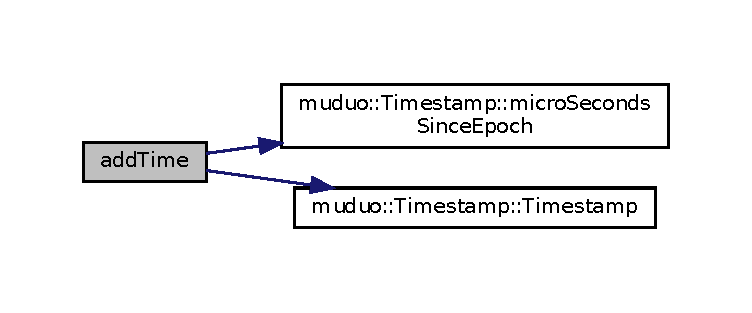
\includegraphics[width=350pt]{namespacemuduo_a4c4a0e85f7b5c4056878cd7cf26a83cb_cgraph}
\end{center}
\end{figure}
这是这个函数的调用关系图\+:
\nopagebreak
\begin{figure}[H]
\begin{center}
\leavevmode
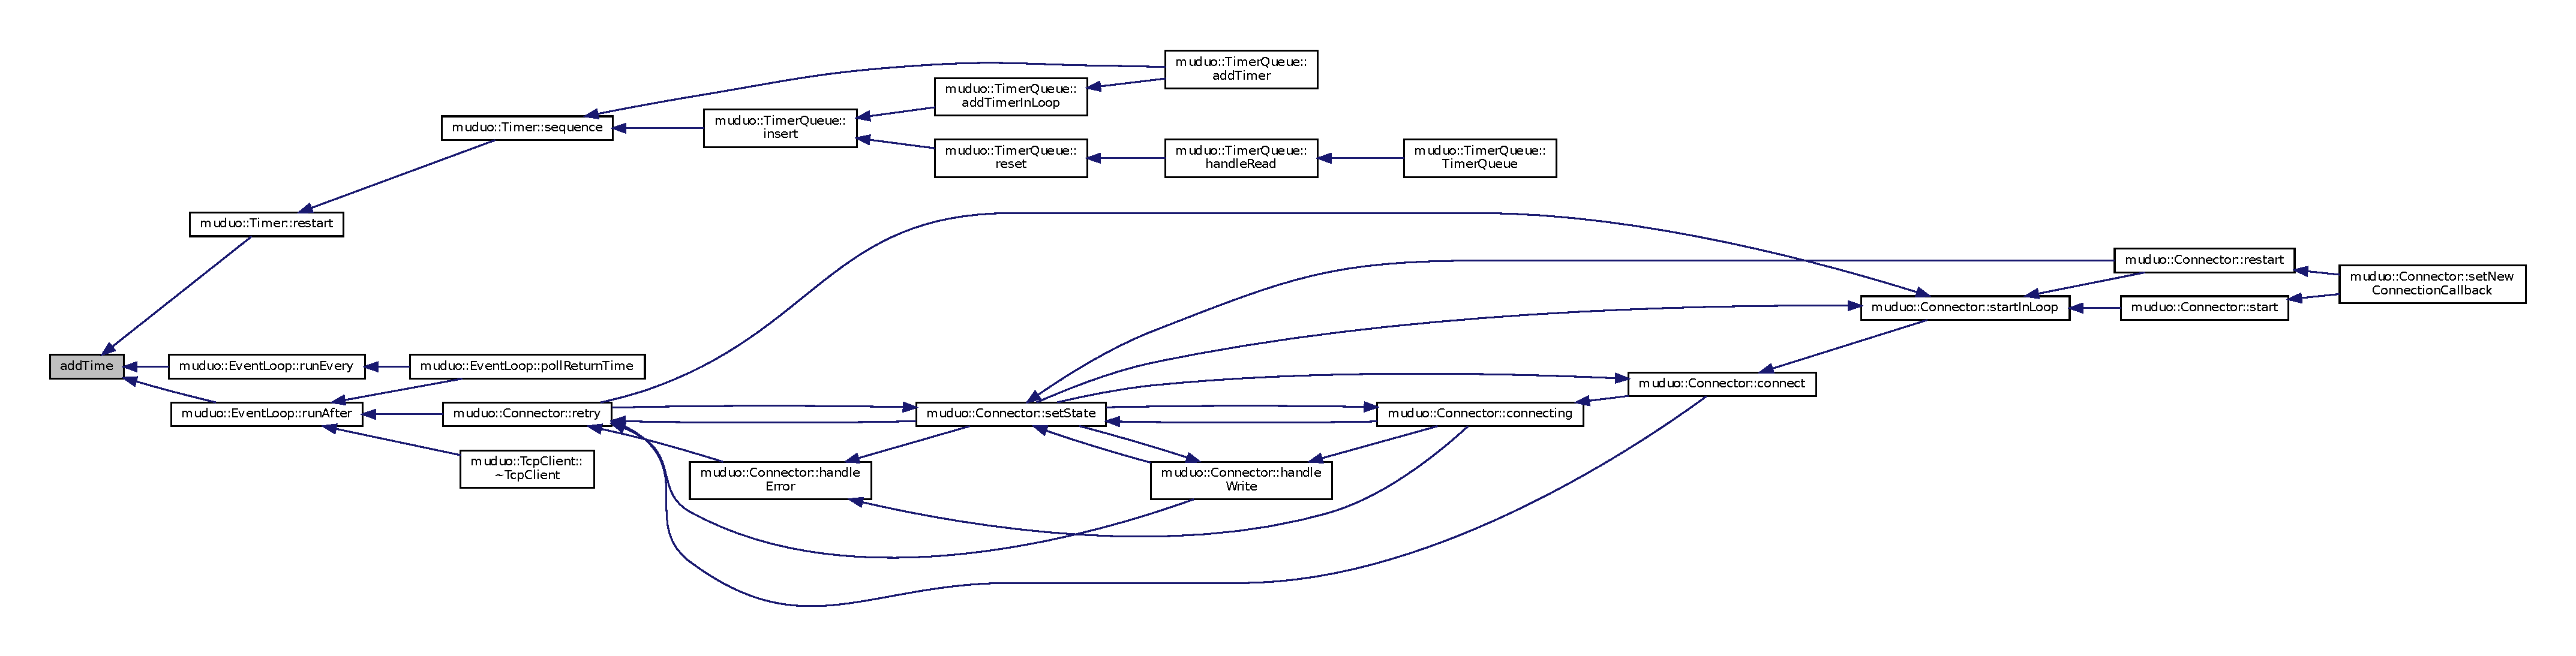
\includegraphics[width=350pt]{namespacemuduo_a4c4a0e85f7b5c4056878cd7cf26a83cb_icgraph}
\end{center}
\end{figure}
\mbox{\Hypertarget{namespacemuduo_a4b813c501ed67387236a1291d1873ab5}\label{namespacemuduo_a4b813c501ed67387236a1291d1873ab5}} 
\index{muduo@{muduo}!Check\+Not\+Null@{Check\+Not\+Null}}
\index{Check\+Not\+Null@{Check\+Not\+Null}!muduo@{muduo}}
\subsubsection{\texorpdfstring{Check\+Not\+Null()}{CheckNotNull()}}
{\footnotesize\ttfamily T$\ast$ muduo\+::\+Check\+Not\+Null (\begin{DoxyParamCaption}\item[{\hyperlink{classmuduo_1_1Logger_1_1SourceFile}{Logger\+::\+Source\+File}}]{file,  }\item[{int}]{line,  }\item[{const char $\ast$}]{names,  }\item[{T $\ast$}]{ptr }\end{DoxyParamCaption})}



在文件 Logging.\+h 第 148 行定义.



参考 Logger\+::\+F\+A\+T\+AL , 以及 Logger\+::\+Logger().

函数调用图\+:
\nopagebreak
\begin{figure}[H]
\begin{center}
\leavevmode
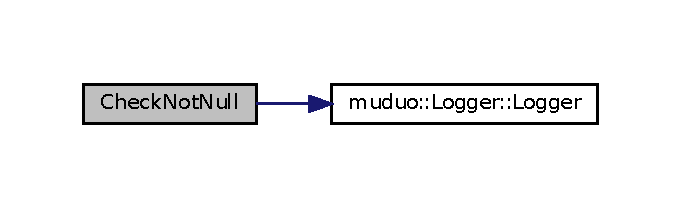
\includegraphics[width=327pt]{namespacemuduo_a4b813c501ed67387236a1291d1873ab5_cgraph}
\end{center}
\end{figure}
\mbox{\Hypertarget{namespacemuduo_a4a5610d86660bbd28e059ebb1ffc8316}\label{namespacemuduo_a4a5610d86660bbd28e059ebb1ffc8316}} 
\index{muduo@{muduo}!down\+\_\+cast@{down\+\_\+cast}}
\index{down\+\_\+cast@{down\+\_\+cast}!muduo@{muduo}}
\subsubsection{\texorpdfstring{down\+\_\+cast()}{down\_cast()}}
{\footnotesize\ttfamily To muduo\+::down\+\_\+cast (\begin{DoxyParamCaption}\item[{From $\ast$}]{f }\end{DoxyParamCaption})\hspace{0.3cm}{\ttfamily [inline]}}



在文件 Types.\+h 第 104 行定义.



参考 implicit\+\_\+cast().

函数调用图\+:
\nopagebreak
\begin{figure}[H]
\begin{center}
\leavevmode
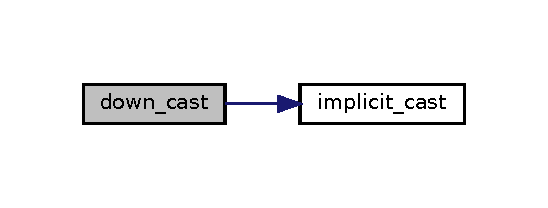
\includegraphics[width=263pt]{namespacemuduo_a4a5610d86660bbd28e059ebb1ffc8316_cgraph}
\end{center}
\end{figure}
\mbox{\Hypertarget{namespacemuduo_a1836aa0a42711172d5598fbfda6fb588}\label{namespacemuduo_a1836aa0a42711172d5598fbfda6fb588}} 
\index{muduo@{muduo}!down\+\_\+pointer\+\_\+cast@{down\+\_\+pointer\+\_\+cast}}
\index{down\+\_\+pointer\+\_\+cast@{down\+\_\+pointer\+\_\+cast}!muduo@{muduo}}
\subsubsection{\texorpdfstring{down\+\_\+pointer\+\_\+cast()}{down\_pointer\_cast()}}
{\footnotesize\ttfamily inline \+::std\+::shared\+\_\+ptr$<$To$>$ muduo\+::down\+\_\+pointer\+\_\+cast (\begin{DoxyParamCaption}\item[{const \+::std\+::shared\+\_\+ptr$<$ From $>$ \&}]{f }\end{DoxyParamCaption})}



在文件 Callbacks.\+h 第 43 行定义.



参考 get\+\_\+pointer() , 以及 implicit\+\_\+cast().

函数调用图\+:
\nopagebreak
\begin{figure}[H]
\begin{center}
\leavevmode
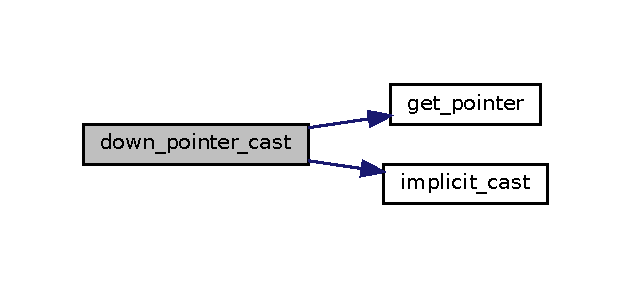
\includegraphics[width=303pt]{namespacemuduo_a1836aa0a42711172d5598fbfda6fb588_cgraph}
\end{center}
\end{figure}
\mbox{\Hypertarget{namespacemuduo_a2ad8a8650556c05bae4c4f449ac6d106}\label{namespacemuduo_a2ad8a8650556c05bae4c4f449ac6d106}} 
\index{muduo@{muduo}!format\+I\+EC@{format\+I\+EC}}
\index{format\+I\+EC@{format\+I\+EC}!muduo@{muduo}}
\subsubsection{\texorpdfstring{format\+I\+E\+C()}{formatIEC()}}
{\footnotesize\ttfamily string muduo\+::format\+I\+EC (\begin{DoxyParamCaption}\item[{int64\+\_\+t}]{n }\end{DoxyParamCaption})}



参考自 operator$<$$<$().

这是这个函数的调用关系图\+:
\nopagebreak
\begin{figure}[H]
\begin{center}
\leavevmode
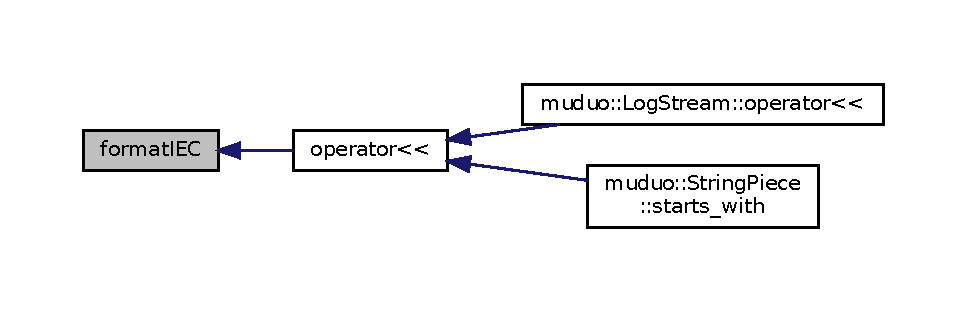
\includegraphics[width=350pt]{namespacemuduo_a2ad8a8650556c05bae4c4f449ac6d106_icgraph}
\end{center}
\end{figure}
\mbox{\Hypertarget{namespacemuduo_a2530c171cac6dda7399a9eb5805e01fa}\label{namespacemuduo_a2530c171cac6dda7399a9eb5805e01fa}} 
\index{muduo@{muduo}!format\+SI@{format\+SI}}
\index{format\+SI@{format\+SI}!muduo@{muduo}}
\subsubsection{\texorpdfstring{format\+S\+I()}{formatSI()}}
{\footnotesize\ttfamily string muduo\+::format\+SI (\begin{DoxyParamCaption}\item[{int64\+\_\+t}]{n }\end{DoxyParamCaption})}



参考自 operator$<$$<$().

这是这个函数的调用关系图\+:
\nopagebreak
\begin{figure}[H]
\begin{center}
\leavevmode
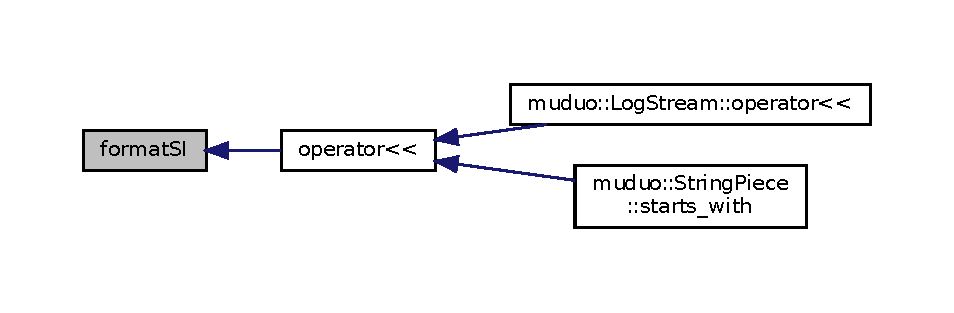
\includegraphics[width=350pt]{namespacemuduo_a2530c171cac6dda7399a9eb5805e01fa_icgraph}
\end{center}
\end{figure}
\mbox{\Hypertarget{namespacemuduo_a98789775449e36c3c0c26004e19ef6bc}\label{namespacemuduo_a98789775449e36c3c0c26004e19ef6bc}} 
\index{muduo@{muduo}!get\+\_\+pointer@{get\+\_\+pointer}}
\index{get\+\_\+pointer@{get\+\_\+pointer}!muduo@{muduo}}
\subsubsection{\texorpdfstring{get\+\_\+pointer()}{get\_pointer()}\hspace{0.1cm}{\footnotesize\ttfamily [1/2]}}
{\footnotesize\ttfamily T$\ast$ muduo\+::get\+\_\+pointer (\begin{DoxyParamCaption}\item[{const std\+::shared\+\_\+ptr$<$ T $>$ \&}]{ptr }\end{DoxyParamCaption})\hspace{0.3cm}{\ttfamily [inline]}}



在文件 Callbacks.\+h 第 29 行定义.



参考自 Tcp\+Connection\+::connect\+Destoryed(), down\+\_\+pointer\+\_\+cast(), Connector\+::remove\+And\+Reset\+Channel(), Tcp\+Server\+::start(), Tcp\+Client\+::\+Tcp\+Client() , 以及 Tcp\+Client\+::$\sim$\+Tcp\+Client().

这是这个函数的调用关系图\+:
\nopagebreak
\begin{figure}[H]
\begin{center}
\leavevmode
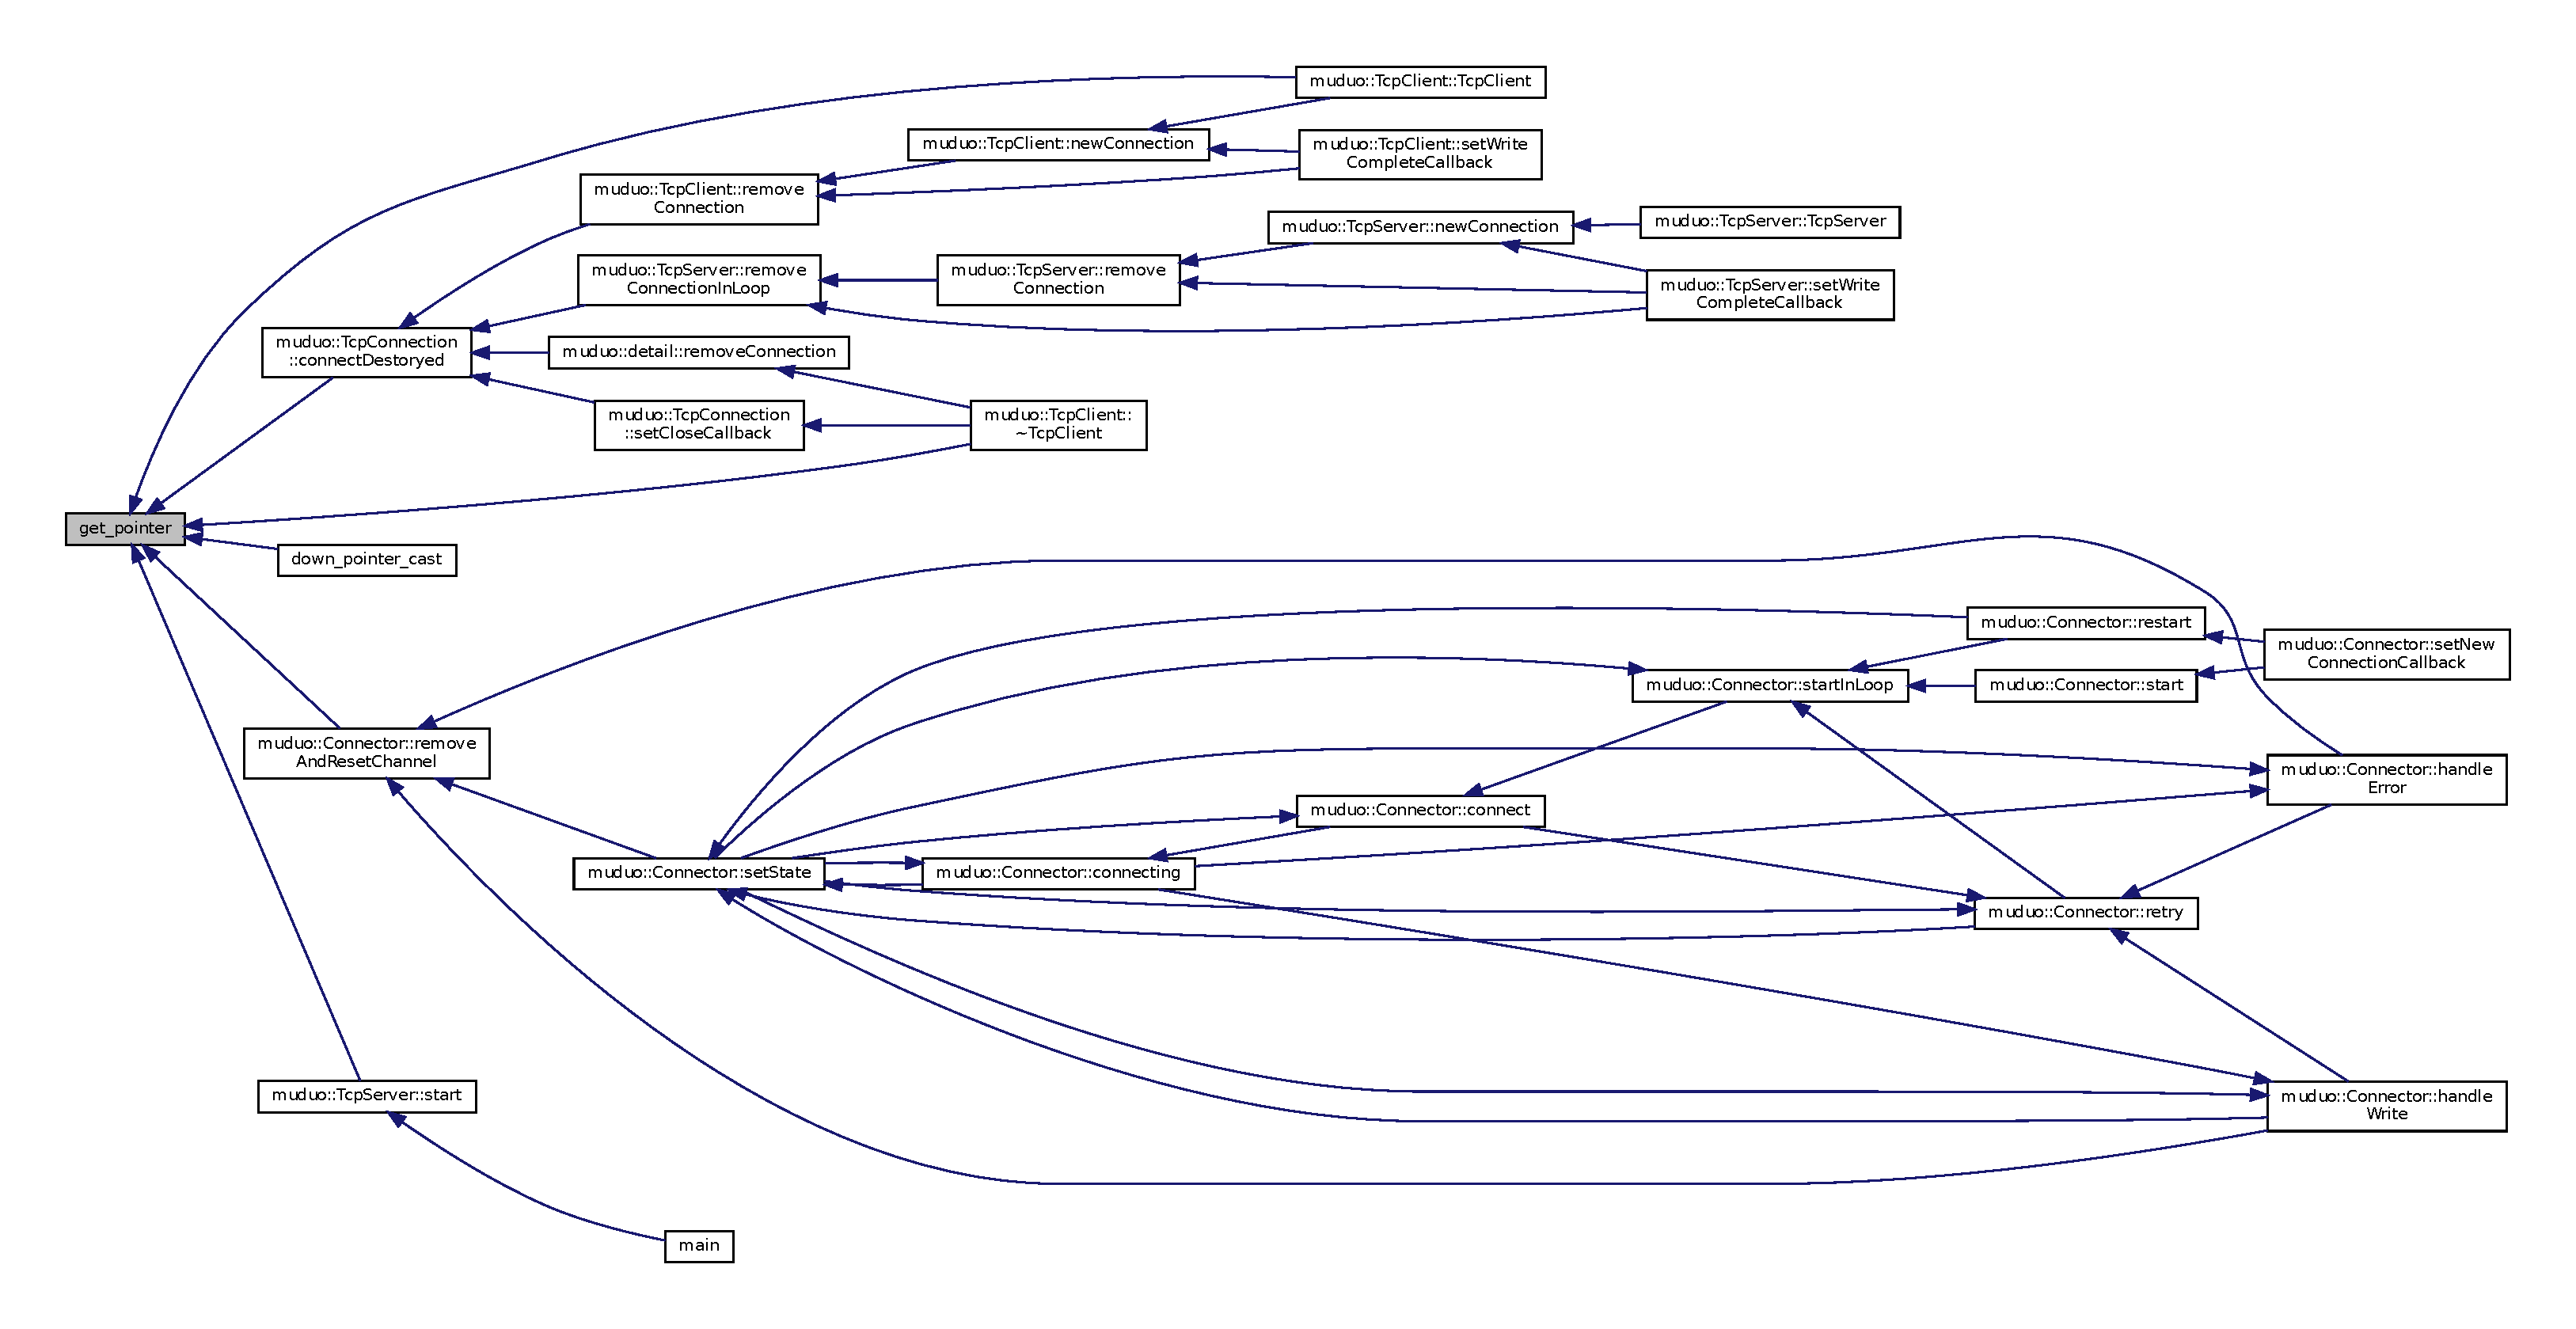
\includegraphics[width=350pt]{namespacemuduo_a98789775449e36c3c0c26004e19ef6bc_icgraph}
\end{center}
\end{figure}
\mbox{\Hypertarget{namespacemuduo_aedcb2cb9b3d8f7bdfabeadec584a691c}\label{namespacemuduo_aedcb2cb9b3d8f7bdfabeadec584a691c}} 
\index{muduo@{muduo}!get\+\_\+pointer@{get\+\_\+pointer}}
\index{get\+\_\+pointer@{get\+\_\+pointer}!muduo@{muduo}}
\subsubsection{\texorpdfstring{get\+\_\+pointer()}{get\_pointer()}\hspace{0.1cm}{\footnotesize\ttfamily [2/2]}}
{\footnotesize\ttfamily T$\ast$ muduo\+::get\+\_\+pointer (\begin{DoxyParamCaption}\item[{const std\+::unique\+\_\+ptr$<$ T $>$ \&}]{ptr }\end{DoxyParamCaption})\hspace{0.3cm}{\ttfamily [inline]}}



在文件 Callbacks.\+h 第 35 行定义.

\mbox{\Hypertarget{namespacemuduo_a72cbcf425db108335295456e8ff9c12b}\label{namespacemuduo_a72cbcf425db108335295456e8ff9c12b}} 
\index{muduo@{muduo}!implicit\+\_\+cast@{implicit\+\_\+cast}}
\index{implicit\+\_\+cast@{implicit\+\_\+cast}!muduo@{muduo}}
\subsubsection{\texorpdfstring{implicit\+\_\+cast()}{implicit\_cast()}}
{\footnotesize\ttfamily To muduo\+::implicit\+\_\+cast (\begin{DoxyParamCaption}\item[{From const \&}]{f }\end{DoxyParamCaption})\hspace{0.3cm}{\ttfamily [inline]}}



在文件 Types.\+h 第 80 行定义.



参考自 down\+\_\+cast() , 以及 down\+\_\+pointer\+\_\+cast().

这是这个函数的调用关系图\+:
\nopagebreak
\begin{figure}[H]
\begin{center}
\leavevmode
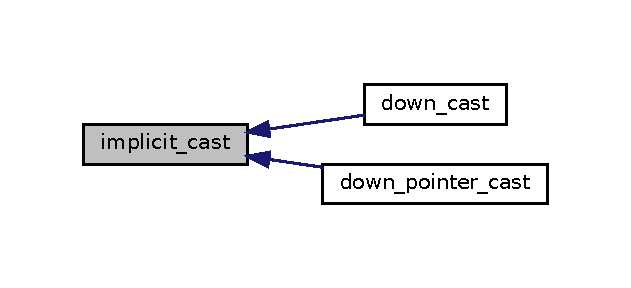
\includegraphics[width=303pt]{namespacemuduo_a72cbcf425db108335295456e8ff9c12b_icgraph}
\end{center}
\end{figure}
\mbox{\Hypertarget{namespacemuduo_ae9dd2c7476408fd8f17491aff0d422f1}\label{namespacemuduo_ae9dd2c7476408fd8f17491aff0d422f1}} 
\index{muduo@{muduo}!make\+Weak\+Callback@{make\+Weak\+Callback}}
\index{make\+Weak\+Callback@{make\+Weak\+Callback}!muduo@{muduo}}
\subsubsection{\texorpdfstring{make\+Weak\+Callback()}{makeWeakCallback()}}
{\footnotesize\ttfamily \hyperlink{classmuduo_1_1WeakCallback}{Weak\+Callback}$<$ C\+L\+A\+SS, A\+R\+G\+S... $>$ make\+Weak\+Callback (\begin{DoxyParamCaption}\item[{const std\+::shared\+\_\+ptr$<$ C\+L\+A\+SS $>$ \&}]{object,  }\item[{void(C\+L\+A\+S\+S\+::$\ast$)(A\+R\+G\+S...)}]{function }\end{DoxyParamCaption})}



在文件 Weak\+Callback.\+h 第 50 行定义.

\mbox{\Hypertarget{namespacemuduo_a8f6d784bddb9d3e0774a665b147758bc}\label{namespacemuduo_a8f6d784bddb9d3e0774a665b147758bc}} 
\index{muduo@{muduo}!mem\+Zero@{mem\+Zero}}
\index{mem\+Zero@{mem\+Zero}!muduo@{muduo}}
\subsubsection{\texorpdfstring{mem\+Zero()}{memZero()}}
{\footnotesize\ttfamily void muduo\+::mem\+Zero (\begin{DoxyParamCaption}\item[{void $\ast$}]{p,  }\item[{size\+\_\+t}]{n }\end{DoxyParamCaption})\hspace{0.3cm}{\ttfamily [inline]}}



在文件 Types.\+h 第 20 行定义.



参考自 Fixed\+Buffer$<$ detail\+::k\+Small\+Buffer $>$\+::bzero().

这是这个函数的调用关系图\+:
\nopagebreak
\begin{figure}[H]
\begin{center}
\leavevmode
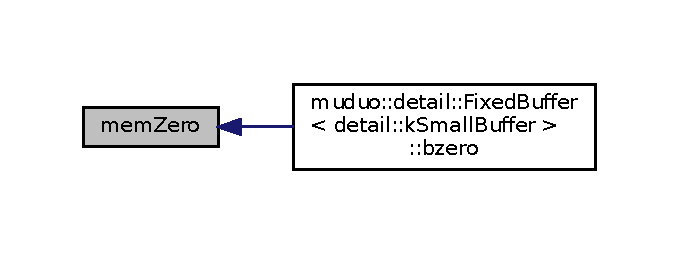
\includegraphics[width=326pt]{namespacemuduo_a8f6d784bddb9d3e0774a665b147758bc_icgraph}
\end{center}
\end{figure}
\mbox{\Hypertarget{namespacemuduo_a7cdae651f87c159c785591256d06740e}\label{namespacemuduo_a7cdae651f87c159c785591256d06740e}} 
\index{muduo@{muduo}!operator$<$@{operator$<$}}
\index{operator$<$@{operator$<$}!muduo@{muduo}}
\subsubsection{\texorpdfstring{operator$<$()}{operator<()}\hspace{0.1cm}{\footnotesize\ttfamily [1/2]}}
{\footnotesize\ttfamily bool muduo\+::operator$<$ (\begin{DoxyParamCaption}\item[{\hyperlink{classmuduo_1_1Timestamp}{Timestamp}}]{lhs,  }\item[{\hyperlink{classmuduo_1_1Timestamp}{Timestamp}}]{rhs }\end{DoxyParamCaption})\hspace{0.3cm}{\ttfamily [inline]}}



在文件 Timestamp.\+h 第 87 行定义.



参考 Timestamp\+::micro\+Seconds\+Since\+Epoch().

函数调用图\+:
\nopagebreak
\begin{figure}[H]
\begin{center}
\leavevmode
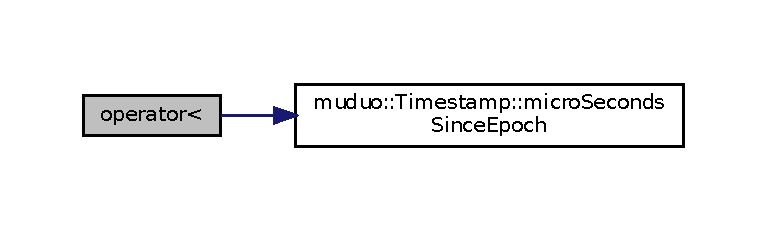
\includegraphics[width=350pt]{namespacemuduo_a7cdae651f87c159c785591256d06740e_cgraph}
\end{center}
\end{figure}
\mbox{\Hypertarget{namespacemuduo_a16d6a8ea1b5e79c94c59f96137b8d26d}\label{namespacemuduo_a16d6a8ea1b5e79c94c59f96137b8d26d}} 
\index{muduo@{muduo}!operator$<$@{operator$<$}}
\index{operator$<$@{operator$<$}!muduo@{muduo}}
\subsubsection{\texorpdfstring{operator$<$()}{operator<()}\hspace{0.1cm}{\footnotesize\ttfamily [2/2]}}
{\footnotesize\ttfamily bool muduo\+::operator$<$ (\begin{DoxyParamCaption}\item[{\hyperlink{classmuduo_1_1Date}{Date}}]{x,  }\item[{\hyperlink{classmuduo_1_1Date}{Date}}]{y }\end{DoxyParamCaption})\hspace{0.3cm}{\ttfamily [inline]}}



在文件 Date.\+h 第 107 行定义.



参考 Date\+::julian\+Day\+Number().

函数调用图\+:
\nopagebreak
\begin{figure}[H]
\begin{center}
\leavevmode
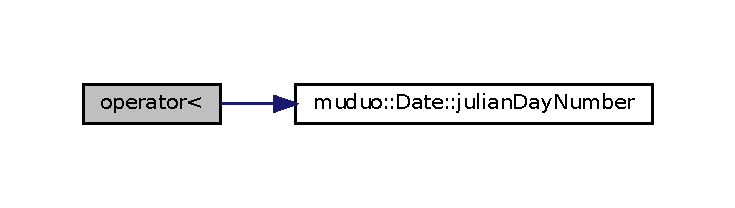
\includegraphics[width=350pt]{namespacemuduo_a16d6a8ea1b5e79c94c59f96137b8d26d_cgraph}
\end{center}
\end{figure}
\mbox{\Hypertarget{namespacemuduo_a8306fbe1f821ddb82e4c161f936695b2}\label{namespacemuduo_a8306fbe1f821ddb82e4c161f936695b2}} 
\index{muduo@{muduo}!operator$<$$<$@{operator$<$$<$}}
\index{operator$<$$<$@{operator$<$$<$}!muduo@{muduo}}
\subsubsection{\texorpdfstring{operator$<$$<$()}{operator<<()}}
{\footnotesize\ttfamily \hyperlink{classmuduo_1_1LogStream}{Log\+Stream}\& muduo\+::operator$<$$<$ (\begin{DoxyParamCaption}\item[{\hyperlink{classmuduo_1_1LogStream}{Log\+Stream} \&}]{s,  }\item[{const \hyperlink{classmuduo_1_1Fmt}{Fmt} \&}]{fmt }\end{DoxyParamCaption})\hspace{0.3cm}{\ttfamily [inline]}}



在文件 Log\+Stream.\+h 第 185 行定义.



参考 Log\+Stream\+::append(), Fmt\+::data(), format\+I\+E\+C(), format\+S\+I() , 以及 Fmt\+::length().



参考自 Log\+Stream\+::operator$<$$<$() , 以及 String\+Piece\+::starts\+\_\+with().

函数调用图\+:
\nopagebreak
\begin{figure}[H]
\begin{center}
\leavevmode
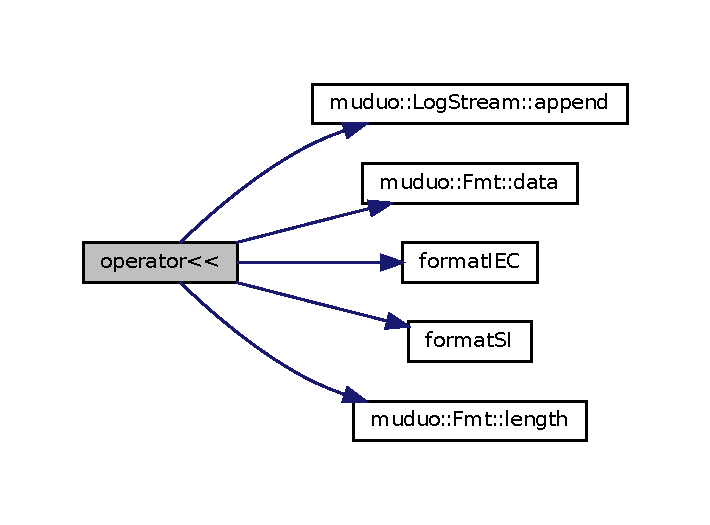
\includegraphics[width=341pt]{namespacemuduo_a8306fbe1f821ddb82e4c161f936695b2_cgraph}
\end{center}
\end{figure}
这是这个函数的调用关系图\+:
\nopagebreak
\begin{figure}[H]
\begin{center}
\leavevmode
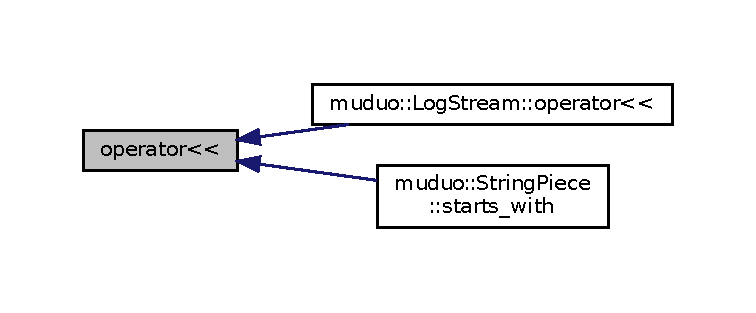
\includegraphics[width=350pt]{namespacemuduo_a8306fbe1f821ddb82e4c161f936695b2_icgraph}
\end{center}
\end{figure}
\mbox{\Hypertarget{namespacemuduo_abf794c2f7edbea7af7ae48632eef1b84}\label{namespacemuduo_abf794c2f7edbea7af7ae48632eef1b84}} 
\index{muduo@{muduo}!operator==@{operator==}}
\index{operator==@{operator==}!muduo@{muduo}}
\subsubsection{\texorpdfstring{operator==()}{operator==()}\hspace{0.1cm}{\footnotesize\ttfamily [1/2]}}
{\footnotesize\ttfamily bool muduo\+::operator== (\begin{DoxyParamCaption}\item[{\hyperlink{classmuduo_1_1Timestamp}{Timestamp}}]{lhs,  }\item[{\hyperlink{classmuduo_1_1Timestamp}{Timestamp}}]{rhs }\end{DoxyParamCaption})\hspace{0.3cm}{\ttfamily [inline]}}



在文件 Timestamp.\+h 第 92 行定义.



参考 Timestamp\+::micro\+Seconds\+Since\+Epoch().

函数调用图\+:
\nopagebreak
\begin{figure}[H]
\begin{center}
\leavevmode
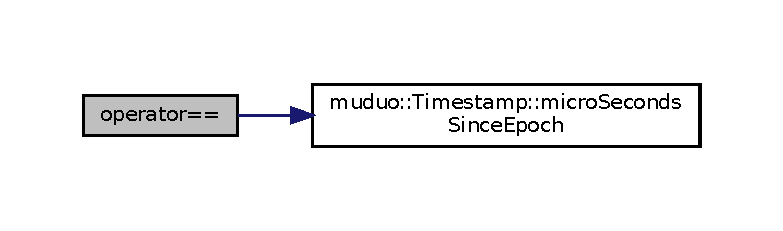
\includegraphics[width=350pt]{namespacemuduo_abf794c2f7edbea7af7ae48632eef1b84_cgraph}
\end{center}
\end{figure}
\mbox{\Hypertarget{namespacemuduo_a0a048e90c15864ab82a55b148bebd144}\label{namespacemuduo_a0a048e90c15864ab82a55b148bebd144}} 
\index{muduo@{muduo}!operator==@{operator==}}
\index{operator==@{operator==}!muduo@{muduo}}
\subsubsection{\texorpdfstring{operator==()}{operator==()}\hspace{0.1cm}{\footnotesize\ttfamily [2/2]}}
{\footnotesize\ttfamily bool muduo\+::operator== (\begin{DoxyParamCaption}\item[{\hyperlink{classmuduo_1_1Date}{Date}}]{x,  }\item[{\hyperlink{classmuduo_1_1Date}{Date}}]{y }\end{DoxyParamCaption})\hspace{0.3cm}{\ttfamily [inline]}}



在文件 Date.\+h 第 112 行定义.



参考 Date\+::julian\+Day\+Number().

函数调用图\+:
\nopagebreak
\begin{figure}[H]
\begin{center}
\leavevmode
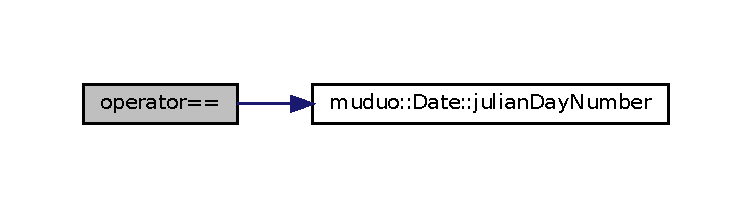
\includegraphics[width=350pt]{namespacemuduo_a0a048e90c15864ab82a55b148bebd144_cgraph}
\end{center}
\end{figure}
\mbox{\Hypertarget{namespacemuduo_a8c7278edf83f347bacf79e36689bf91c}\label{namespacemuduo_a8c7278edf83f347bacf79e36689bf91c}} 
\index{muduo@{muduo}!strerror\+\_\+tl@{strerror\+\_\+tl}}
\index{strerror\+\_\+tl@{strerror\+\_\+tl}!muduo@{muduo}}
\subsubsection{\texorpdfstring{strerror\+\_\+tl()}{strerror\_tl()}}
{\footnotesize\ttfamily const char$\ast$ muduo\+::strerror\+\_\+tl (\begin{DoxyParamCaption}\item[{int}]{saved\+Errno }\end{DoxyParamCaption})}



参考自 Connector\+::handle\+Error(), Tcp\+Connection\+::handle\+Error() , 以及 Connector\+::handle\+Write().

这是这个函数的调用关系图\+:
\nopagebreak
\begin{figure}[H]
\begin{center}
\leavevmode
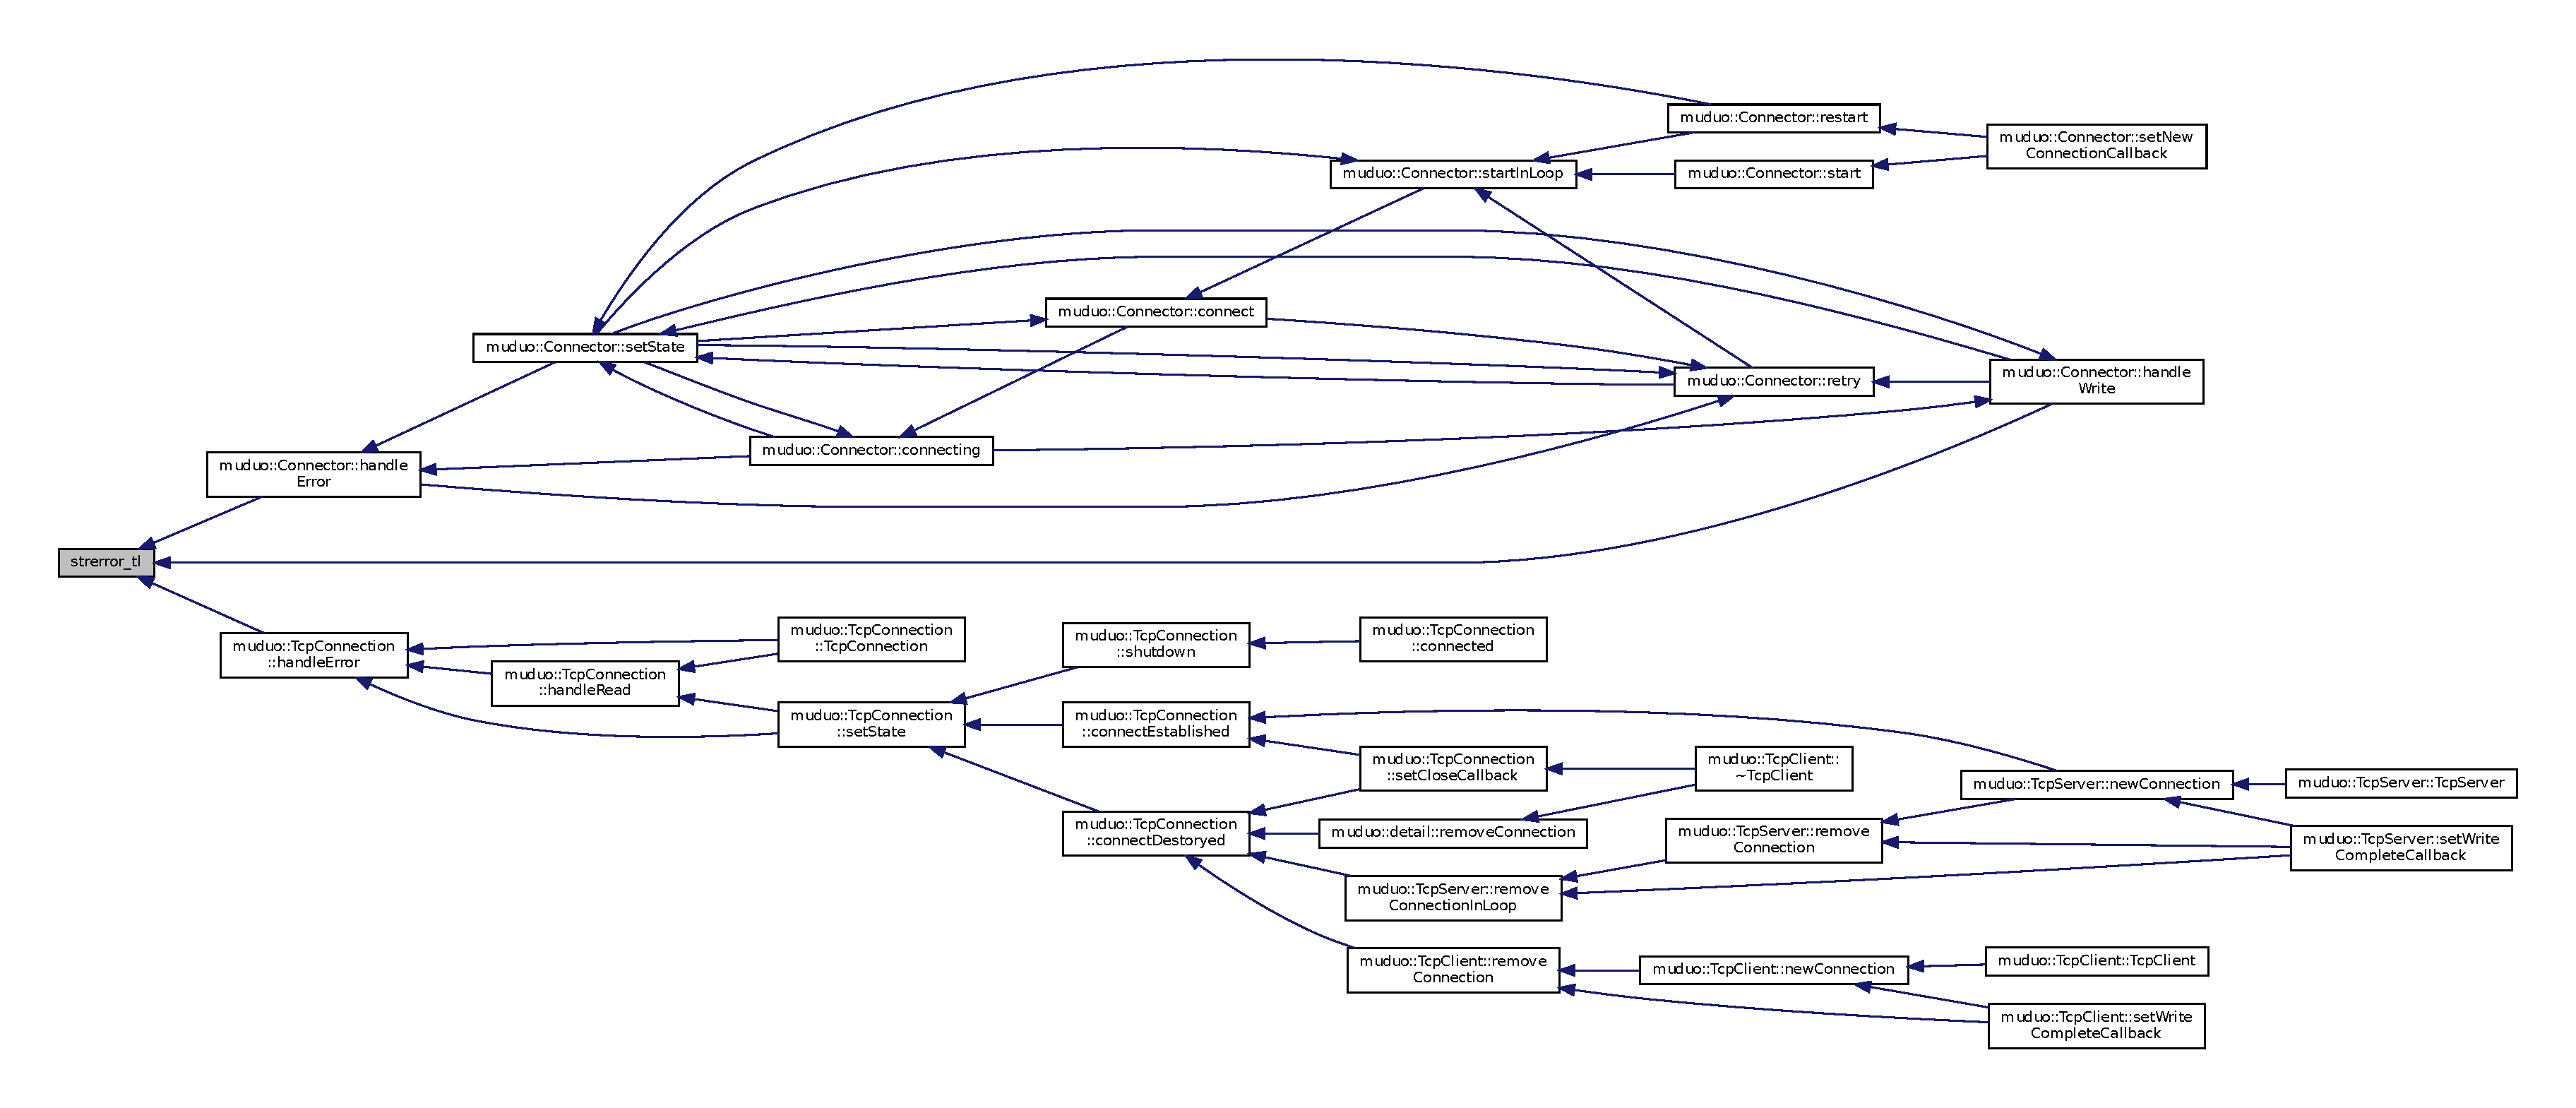
\includegraphics[width=350pt]{namespacemuduo_a8c7278edf83f347bacf79e36689bf91c_icgraph}
\end{center}
\end{figure}
\mbox{\Hypertarget{namespacemuduo_a6f7c17d86f2474f297b3b9e54b500907}\label{namespacemuduo_a6f7c17d86f2474f297b3b9e54b500907}} 
\index{muduo@{muduo}!time\+Difference@{time\+Difference}}
\index{time\+Difference@{time\+Difference}!muduo@{muduo}}
\subsubsection{\texorpdfstring{time\+Difference()}{timeDifference()}}
{\footnotesize\ttfamily double muduo\+::time\+Difference (\begin{DoxyParamCaption}\item[{\hyperlink{classmuduo_1_1Timestamp}{Timestamp}}]{high,  }\item[{\hyperlink{classmuduo_1_1Timestamp}{Timestamp}}]{low }\end{DoxyParamCaption})\hspace{0.3cm}{\ttfamily [inline]}}

Gets time difference of two timestamps, result in seconds.


\begin{DoxyParams}{参数}
{\em high,low} & \\
\hline
\end{DoxyParams}
\begin{DoxyReturn}{返回}
(high-\/low) in seconds {\ttfamily double} has 52-\/bit precision, enough for one-\/microsecond resolution for next 100 years. 
\end{DoxyReturn}


在文件 Timestamp.\+h 第 104 行定义.



参考 Timestamp\+::k\+Micro\+Seconds\+Per\+Second , 以及 Timestamp\+::micro\+Seconds\+Since\+Epoch().

函数调用图\+:
\nopagebreak
\begin{figure}[H]
\begin{center}
\leavevmode

\includegraphics[width=350pt]{namespacemuduo_a6f7c17d86f2474f297b3b9e54b500907_cgraph}
\end{center}
\end{figure}


\subsection{变量说明}
\mbox{\Hypertarget{namespacemuduo_ac758fb9f0d1703994b7e23772d09f183}\label{namespacemuduo_ac758fb9f0d1703994b7e23772d09f183}} 
\index{muduo@{muduo}!g\+\_\+log\+Level@{g\+\_\+log\+Level}}
\index{g\+\_\+log\+Level@{g\+\_\+log\+Level}!muduo@{muduo}}
\subsubsection{\texorpdfstring{g\+\_\+log\+Level}{g\_logLevel}}
{\footnotesize\ttfamily \hyperlink{classmuduo_1_1Logger_aca1fd1d8935433e6ba2e3918214e07f9}{Logger\+::\+Log\+Level} g\+\_\+log\+Level}



参考自 Logger\+::log\+Level().


\hypertarget{namespacemuduo_1_1CurrentThread}{}\section{muduo\+:\+:Current\+Thread 命名空间参考}
\label{namespacemuduo_1_1CurrentThread}\index{muduo\+::\+Current\+Thread@{muduo\+::\+Current\+Thread}}
\subsection*{函数}
\begin{DoxyCompactItemize}
\item 
void \hyperlink{namespacemuduo_1_1CurrentThread_a09cc852243e579266304c5e31f744929}{cache\+Tid} ()
\item 
int \hyperlink{namespacemuduo_1_1CurrentThread_a27129392a2d642e96188636257bf13ca}{tid} ()
\item 
const char $\ast$ \hyperlink{namespacemuduo_1_1CurrentThread_a66a1e1728583966e9568ae57562a6e93}{tid\+String} ()
\item 
int \hyperlink{namespacemuduo_1_1CurrentThread_a8f000c3381de23423f1c582b116f8b81}{tid\+String\+Length} ()
\item 
const char $\ast$ \hyperlink{namespacemuduo_1_1CurrentThread_adc8b0cfe3a876d8edf272f982ea2c014}{name} ()
\item 
bool \hyperlink{namespacemuduo_1_1CurrentThread_ad8869cd6e09d4440fae5d6698558b3a5}{is\+Main\+Thread} ()
\item 
void \hyperlink{namespacemuduo_1_1CurrentThread_ab625c2286c356d09b66b9ab043946fd1}{sleep\+Usec} (int64\+\_\+t usec)
\item 
string \hyperlink{namespacemuduo_1_1CurrentThread_adb3a86b79370bd58610e2b8942980edf}{stack\+Trace} (bool demangle)
\end{DoxyCompactItemize}
\subsection*{变量}
\begin{DoxyCompactItemize}
\item 
\+\_\+\+\_\+thread int \hyperlink{namespacemuduo_1_1CurrentThread_a0ac6156a2e940999b6e5079f74aed168}{t\+\_\+cached\+Tid}
\item 
\+\_\+\+\_\+thread char \hyperlink{namespacemuduo_1_1CurrentThread_a2d20a2a5e4356ebe49586292d41e6194}{t\+\_\+tid\+String} \mbox{[}32\mbox{]}
\item 
\+\_\+\+\_\+thread int \hyperlink{namespacemuduo_1_1CurrentThread_a9c737bf86b45092ffa7d2eba19767a50}{t\+\_\+tid\+String\+Length}
\item 
\+\_\+\+\_\+thread const char $\ast$ \hyperlink{namespacemuduo_1_1CurrentThread_a34c6e52202ddb3c43a4af8ad4b36e3f9}{t\+\_\+thread\+Name}
\end{DoxyCompactItemize}


\subsection{函数说明}
\mbox{\Hypertarget{namespacemuduo_1_1CurrentThread_a09cc852243e579266304c5e31f744929}\label{namespacemuduo_1_1CurrentThread_a09cc852243e579266304c5e31f744929}} 
\index{muduo\+::\+Current\+Thread@{muduo\+::\+Current\+Thread}!cache\+Tid@{cache\+Tid}}
\index{cache\+Tid@{cache\+Tid}!muduo\+::\+Current\+Thread@{muduo\+::\+Current\+Thread}}
\subsubsection{\texorpdfstring{cache\+Tid()}{cacheTid()}}
{\footnotesize\ttfamily void muduo\+::\+Current\+Thread\+::cache\+Tid (\begin{DoxyParamCaption}{ }\end{DoxyParamCaption})}



参考自 tid().

这是这个函数的调用关系图\+:
\nopagebreak
\begin{figure}[H]
\begin{center}
\leavevmode
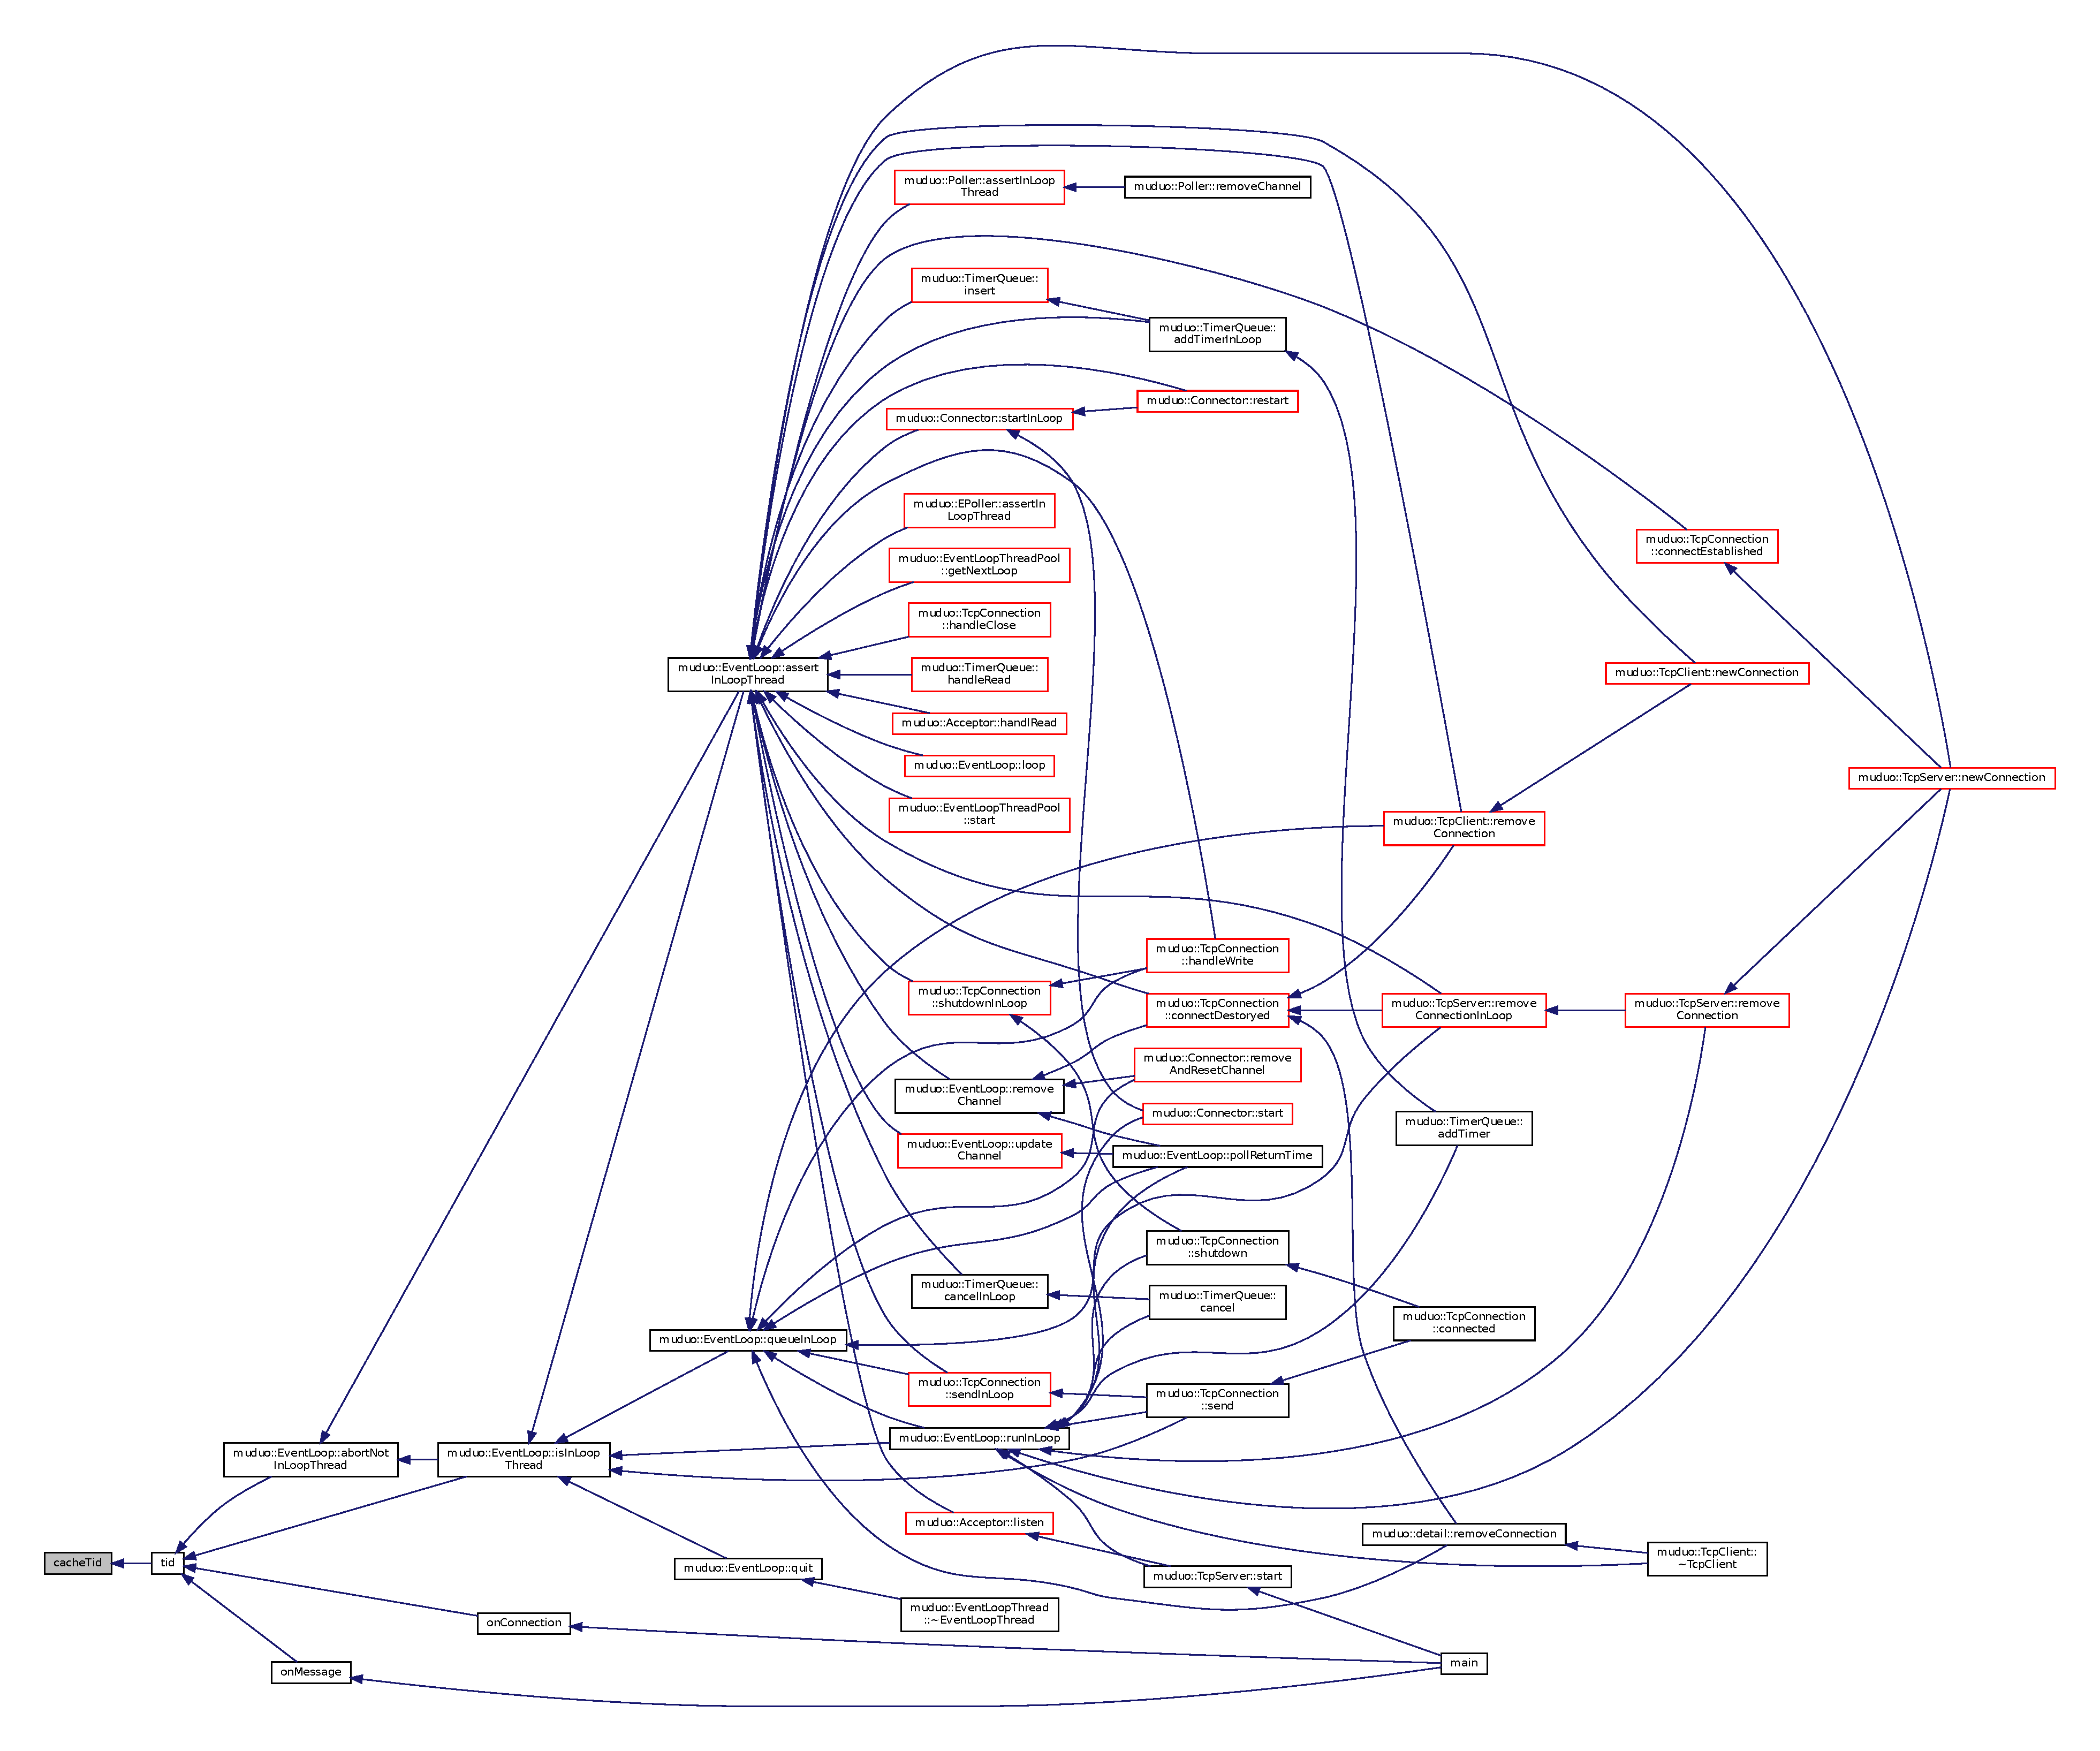
\includegraphics[width=350pt]{namespacemuduo_1_1CurrentThread_a09cc852243e579266304c5e31f744929_icgraph}
\end{center}
\end{figure}
\mbox{\Hypertarget{namespacemuduo_1_1CurrentThread_ad8869cd6e09d4440fae5d6698558b3a5}\label{namespacemuduo_1_1CurrentThread_ad8869cd6e09d4440fae5d6698558b3a5}} 
\index{muduo\+::\+Current\+Thread@{muduo\+::\+Current\+Thread}!is\+Main\+Thread@{is\+Main\+Thread}}
\index{is\+Main\+Thread@{is\+Main\+Thread}!muduo\+::\+Current\+Thread@{muduo\+::\+Current\+Thread}}
\subsubsection{\texorpdfstring{is\+Main\+Thread()}{isMainThread()}}
{\footnotesize\ttfamily bool muduo\+::\+Current\+Thread\+::is\+Main\+Thread (\begin{DoxyParamCaption}{ }\end{DoxyParamCaption})}



参考自 name().

这是这个函数的调用关系图\+:
\nopagebreak
\begin{figure}[H]
\begin{center}
\leavevmode
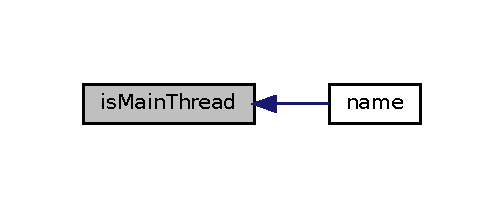
\includegraphics[width=242pt]{namespacemuduo_1_1CurrentThread_ad8869cd6e09d4440fae5d6698558b3a5_icgraph}
\end{center}
\end{figure}
\mbox{\Hypertarget{namespacemuduo_1_1CurrentThread_adc8b0cfe3a876d8edf272f982ea2c014}\label{namespacemuduo_1_1CurrentThread_adc8b0cfe3a876d8edf272f982ea2c014}} 
\index{muduo\+::\+Current\+Thread@{muduo\+::\+Current\+Thread}!name@{name}}
\index{name@{name}!muduo\+::\+Current\+Thread@{muduo\+::\+Current\+Thread}}
\subsubsection{\texorpdfstring{name()}{name()}}
{\footnotesize\ttfamily const char$\ast$ muduo\+::\+Current\+Thread\+::name (\begin{DoxyParamCaption}{ }\end{DoxyParamCaption})\hspace{0.3cm}{\ttfamily [inline]}}



在文件 Current\+Thread.\+h 第 41 行定义.



参考 is\+Main\+Thread(), sleep\+Usec(), stack\+Trace() , 以及 t\+\_\+thread\+Name.

函数调用图\+:
\nopagebreak
\begin{figure}[H]
\begin{center}
\leavevmode
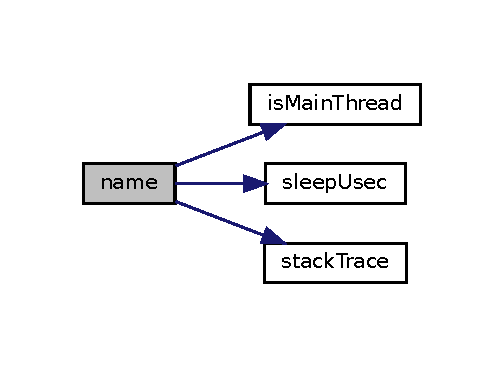
\includegraphics[width=242pt]{namespacemuduo_1_1CurrentThread_adc8b0cfe3a876d8edf272f982ea2c014_cgraph}
\end{center}
\end{figure}
\mbox{\Hypertarget{namespacemuduo_1_1CurrentThread_ab625c2286c356d09b66b9ab043946fd1}\label{namespacemuduo_1_1CurrentThread_ab625c2286c356d09b66b9ab043946fd1}} 
\index{muduo\+::\+Current\+Thread@{muduo\+::\+Current\+Thread}!sleep\+Usec@{sleep\+Usec}}
\index{sleep\+Usec@{sleep\+Usec}!muduo\+::\+Current\+Thread@{muduo\+::\+Current\+Thread}}
\subsubsection{\texorpdfstring{sleep\+Usec()}{sleepUsec()}}
{\footnotesize\ttfamily void muduo\+::\+Current\+Thread\+::sleep\+Usec (\begin{DoxyParamCaption}\item[{int64\+\_\+t}]{usec }\end{DoxyParamCaption})}



参考自 name().

这是这个函数的调用关系图\+:
\nopagebreak
\begin{figure}[H]
\begin{center}
\leavevmode
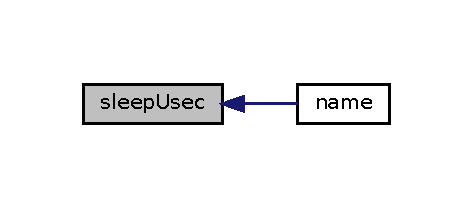
\includegraphics[width=227pt]{namespacemuduo_1_1CurrentThread_ab625c2286c356d09b66b9ab043946fd1_icgraph}
\end{center}
\end{figure}
\mbox{\Hypertarget{namespacemuduo_1_1CurrentThread_adb3a86b79370bd58610e2b8942980edf}\label{namespacemuduo_1_1CurrentThread_adb3a86b79370bd58610e2b8942980edf}} 
\index{muduo\+::\+Current\+Thread@{muduo\+::\+Current\+Thread}!stack\+Trace@{stack\+Trace}}
\index{stack\+Trace@{stack\+Trace}!muduo\+::\+Current\+Thread@{muduo\+::\+Current\+Thread}}
\subsubsection{\texorpdfstring{stack\+Trace()}{stackTrace()}}
{\footnotesize\ttfamily string muduo\+::\+Current\+Thread\+::stack\+Trace (\begin{DoxyParamCaption}\item[{bool}]{demangle }\end{DoxyParamCaption})}



参考自 name().

这是这个函数的调用关系图\+:
\nopagebreak
\begin{figure}[H]
\begin{center}
\leavevmode
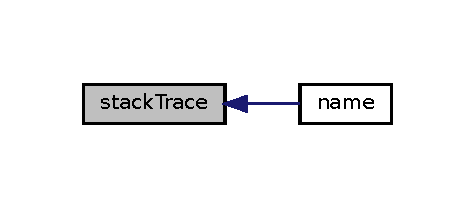
\includegraphics[width=228pt]{namespacemuduo_1_1CurrentThread_adb3a86b79370bd58610e2b8942980edf_icgraph}
\end{center}
\end{figure}
\mbox{\Hypertarget{namespacemuduo_1_1CurrentThread_a27129392a2d642e96188636257bf13ca}\label{namespacemuduo_1_1CurrentThread_a27129392a2d642e96188636257bf13ca}} 
\index{muduo\+::\+Current\+Thread@{muduo\+::\+Current\+Thread}!tid@{tid}}
\index{tid@{tid}!muduo\+::\+Current\+Thread@{muduo\+::\+Current\+Thread}}
\subsubsection{\texorpdfstring{tid()}{tid()}}
{\footnotesize\ttfamily int muduo\+::\+Current\+Thread\+::tid (\begin{DoxyParamCaption}{ }\end{DoxyParamCaption})\hspace{0.3cm}{\ttfamily [inline]}}



在文件 Current\+Thread.\+h 第 22 行定义.



参考 cache\+Tid() , 以及 t\+\_\+cached\+Tid.



参考自 Event\+Loop\+::abort\+Not\+In\+Loop\+Thread(), Event\+Loop\+::is\+In\+Loop\+Thread(), on\+Connection() , 以及 on\+Message().

函数调用图\+:
\nopagebreak
\begin{figure}[H]
\begin{center}
\leavevmode
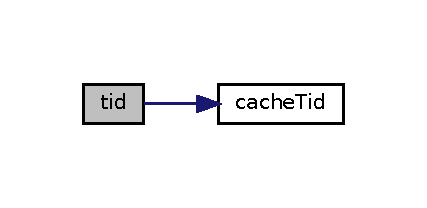
\includegraphics[width=205pt]{namespacemuduo_1_1CurrentThread_a27129392a2d642e96188636257bf13ca_cgraph}
\end{center}
\end{figure}
这是这个函数的调用关系图\+:
\nopagebreak
\begin{figure}[H]
\begin{center}
\leavevmode
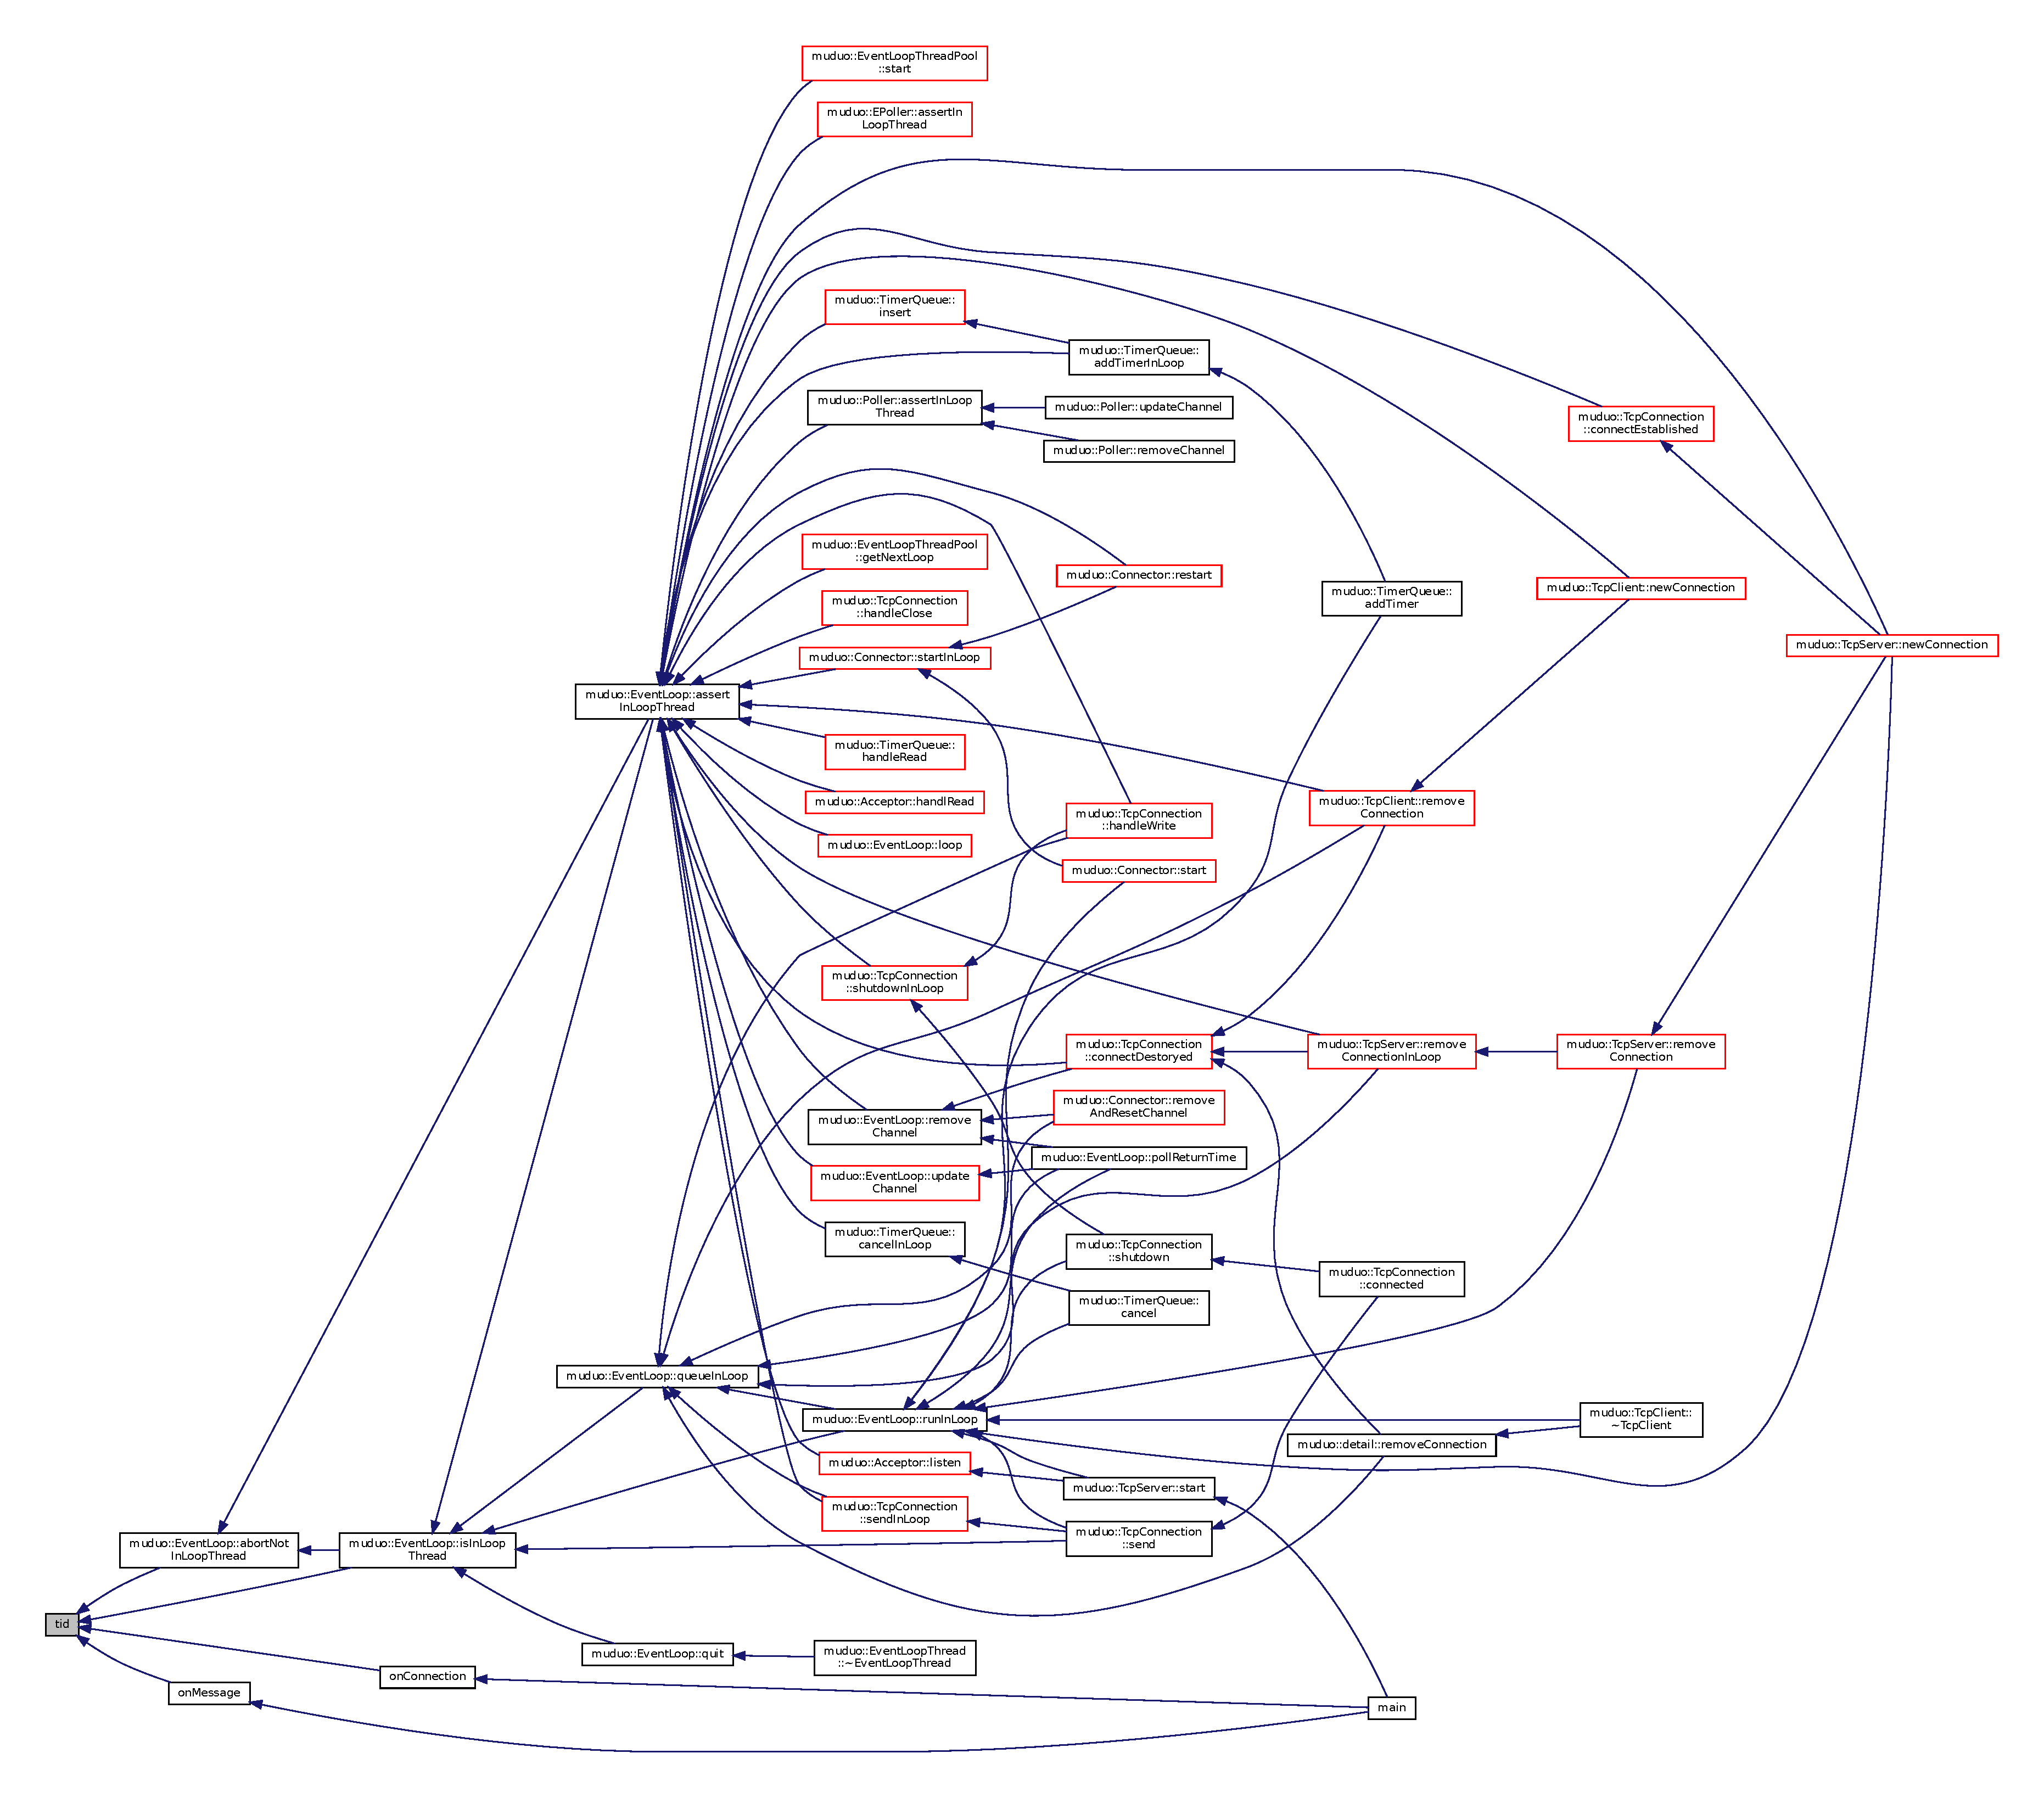
\includegraphics[width=350pt]{namespacemuduo_1_1CurrentThread_a27129392a2d642e96188636257bf13ca_icgraph}
\end{center}
\end{figure}
\mbox{\Hypertarget{namespacemuduo_1_1CurrentThread_a66a1e1728583966e9568ae57562a6e93}\label{namespacemuduo_1_1CurrentThread_a66a1e1728583966e9568ae57562a6e93}} 
\index{muduo\+::\+Current\+Thread@{muduo\+::\+Current\+Thread}!tid\+String@{tid\+String}}
\index{tid\+String@{tid\+String}!muduo\+::\+Current\+Thread@{muduo\+::\+Current\+Thread}}
\subsubsection{\texorpdfstring{tid\+String()}{tidString()}}
{\footnotesize\ttfamily const char$\ast$ muduo\+::\+Current\+Thread\+::tid\+String (\begin{DoxyParamCaption}{ }\end{DoxyParamCaption})\hspace{0.3cm}{\ttfamily [inline]}}



在文件 Current\+Thread.\+h 第 31 行定义.



参考 t\+\_\+tid\+String.

\mbox{\Hypertarget{namespacemuduo_1_1CurrentThread_a8f000c3381de23423f1c582b116f8b81}\label{namespacemuduo_1_1CurrentThread_a8f000c3381de23423f1c582b116f8b81}} 
\index{muduo\+::\+Current\+Thread@{muduo\+::\+Current\+Thread}!tid\+String\+Length@{tid\+String\+Length}}
\index{tid\+String\+Length@{tid\+String\+Length}!muduo\+::\+Current\+Thread@{muduo\+::\+Current\+Thread}}
\subsubsection{\texorpdfstring{tid\+String\+Length()}{tidStringLength()}}
{\footnotesize\ttfamily int muduo\+::\+Current\+Thread\+::tid\+String\+Length (\begin{DoxyParamCaption}{ }\end{DoxyParamCaption})\hspace{0.3cm}{\ttfamily [inline]}}



在文件 Current\+Thread.\+h 第 36 行定义.



参考 t\+\_\+tid\+String\+Length.



\subsection{变量说明}
\mbox{\Hypertarget{namespacemuduo_1_1CurrentThread_a0ac6156a2e940999b6e5079f74aed168}\label{namespacemuduo_1_1CurrentThread_a0ac6156a2e940999b6e5079f74aed168}} 
\index{muduo\+::\+Current\+Thread@{muduo\+::\+Current\+Thread}!t\+\_\+cached\+Tid@{t\+\_\+cached\+Tid}}
\index{t\+\_\+cached\+Tid@{t\+\_\+cached\+Tid}!muduo\+::\+Current\+Thread@{muduo\+::\+Current\+Thread}}
\subsubsection{\texorpdfstring{t\+\_\+cached\+Tid}{t\_cachedTid}}
{\footnotesize\ttfamily \+\_\+\+\_\+thread int t\+\_\+cached\+Tid}



参考自 tid().

\mbox{\Hypertarget{namespacemuduo_1_1CurrentThread_a34c6e52202ddb3c43a4af8ad4b36e3f9}\label{namespacemuduo_1_1CurrentThread_a34c6e52202ddb3c43a4af8ad4b36e3f9}} 
\index{muduo\+::\+Current\+Thread@{muduo\+::\+Current\+Thread}!t\+\_\+thread\+Name@{t\+\_\+thread\+Name}}
\index{t\+\_\+thread\+Name@{t\+\_\+thread\+Name}!muduo\+::\+Current\+Thread@{muduo\+::\+Current\+Thread}}
\subsubsection{\texorpdfstring{t\+\_\+thread\+Name}{t\_threadName}}
{\footnotesize\ttfamily \+\_\+\+\_\+thread const char$\ast$ t\+\_\+thread\+Name}



参考自 name().

\mbox{\Hypertarget{namespacemuduo_1_1CurrentThread_a2d20a2a5e4356ebe49586292d41e6194}\label{namespacemuduo_1_1CurrentThread_a2d20a2a5e4356ebe49586292d41e6194}} 
\index{muduo\+::\+Current\+Thread@{muduo\+::\+Current\+Thread}!t\+\_\+tid\+String@{t\+\_\+tid\+String}}
\index{t\+\_\+tid\+String@{t\+\_\+tid\+String}!muduo\+::\+Current\+Thread@{muduo\+::\+Current\+Thread}}
\subsubsection{\texorpdfstring{t\+\_\+tid\+String}{t\_tidString}}
{\footnotesize\ttfamily \+\_\+\+\_\+thread char t\+\_\+tid\+String\mbox{[}32\mbox{]}}



参考自 tid\+String().

\mbox{\Hypertarget{namespacemuduo_1_1CurrentThread_a9c737bf86b45092ffa7d2eba19767a50}\label{namespacemuduo_1_1CurrentThread_a9c737bf86b45092ffa7d2eba19767a50}} 
\index{muduo\+::\+Current\+Thread@{muduo\+::\+Current\+Thread}!t\+\_\+tid\+String\+Length@{t\+\_\+tid\+String\+Length}}
\index{t\+\_\+tid\+String\+Length@{t\+\_\+tid\+String\+Length}!muduo\+::\+Current\+Thread@{muduo\+::\+Current\+Thread}}
\subsubsection{\texorpdfstring{t\+\_\+tid\+String\+Length}{t\_tidStringLength}}
{\footnotesize\ttfamily \+\_\+\+\_\+thread int t\+\_\+tid\+String\+Length}



参考自 tid\+String\+Length().


\hypertarget{namespacemuduo_1_1detail}{}\section{muduo\+:\+:detail 命名空间参考}
\label{namespacemuduo_1_1detail}\index{muduo\+::detail@{muduo\+::detail}}
\subsection*{类}
\begin{DoxyCompactItemize}
\item 
class \hyperlink{classmuduo_1_1detail_1_1AtomicIntegerT}{Atomic\+IntegerT}
\item 
class \hyperlink{classmuduo_1_1detail_1_1FixedBuffer}{Fixed\+Buffer}
\item 
struct \hyperlink{structmuduo_1_1detail_1_1has__no__destroy}{has\+\_\+no\+\_\+destroy}
\end{DoxyCompactItemize}
\subsection*{函数}
\begin{DoxyCompactItemize}
\item 
void \hyperlink{namespacemuduo_1_1detail_ae3e6bfc20f665df13eeb2ebc3c91abce}{remove\+Connection} (\hyperlink{classmuduo_1_1EventLoop}{Event\+Loop} $\ast$loop, const \hyperlink{namespacemuduo_a40c45128e9700d337d92f3cbb8dd4a0a}{Tcp\+Connection\+Ptr} \&conn)
\item 
void \hyperlink{namespacemuduo_1_1detail_ab9f5e26fda4b27382acd5a0740a83137}{remove\+Connector} (const \hyperlink{namespacemuduo_a144f8adea97b4c9ac75c439f6d87ae29}{Connector\+Ptr} \&connector)
\item 
int \hyperlink{namespacemuduo_1_1detail_af278c30c3aaaf596fb0d2211bac2ff52}{create\+Timerfd} ()
\item 
struct timespec \hyperlink{namespacemuduo_1_1detail_a14924335d79da967a69c650af3002c77}{how\+Much\+Time\+From\+Now} (\hyperlink{classmuduo_1_1Timestamp}{Timestamp} when)
\item 
void \hyperlink{namespacemuduo_1_1detail_a08d79eafe298b7df1941adb4105bf75a}{read\+Timerfd} (int timerfd, \hyperlink{classmuduo_1_1Timestamp}{Timestamp} now)
\item 
void \hyperlink{namespacemuduo_1_1detail_a2a30bb501e8d9bb2da91ab353d1bc6fd}{reset\+Timerfd} (int timerfd, \hyperlink{classmuduo_1_1Timestamp}{Timestamp} expiration)
\end{DoxyCompactItemize}
\subsection*{变量}
\begin{DoxyCompactItemize}
\item 
const int \hyperlink{namespacemuduo_1_1detail_a01441c3dba82e5d4bad1ce2b39ff576b}{k\+Small\+Buffer} = 4000
\item 
const int \hyperlink{namespacemuduo_1_1detail_a72d89caa2e467f089bb6cc480d73b884}{k\+Large\+Buffer} = 4000$\ast$1000
\end{DoxyCompactItemize}


\subsection{函数说明}
\mbox{\Hypertarget{namespacemuduo_1_1detail_af278c30c3aaaf596fb0d2211bac2ff52}\label{namespacemuduo_1_1detail_af278c30c3aaaf596fb0d2211bac2ff52}} 
\index{muduo\+::detail@{muduo\+::detail}!create\+Timerfd@{create\+Timerfd}}
\index{create\+Timerfd@{create\+Timerfd}!muduo\+::detail@{muduo\+::detail}}
\subsubsection{\texorpdfstring{create\+Timerfd()}{createTimerfd()}}
{\footnotesize\ttfamily int muduo\+::detail\+::create\+Timerfd (\begin{DoxyParamCaption}{ }\end{DoxyParamCaption})}



在文件 Timer\+Queue.\+cc 第 17 行定义.



参考 L\+O\+G\+\_\+\+S\+Y\+S\+F\+A\+T\+AL.

\mbox{\Hypertarget{namespacemuduo_1_1detail_a14924335d79da967a69c650af3002c77}\label{namespacemuduo_1_1detail_a14924335d79da967a69c650af3002c77}} 
\index{muduo\+::detail@{muduo\+::detail}!how\+Much\+Time\+From\+Now@{how\+Much\+Time\+From\+Now}}
\index{how\+Much\+Time\+From\+Now@{how\+Much\+Time\+From\+Now}!muduo\+::detail@{muduo\+::detail}}
\subsubsection{\texorpdfstring{how\+Much\+Time\+From\+Now()}{howMuchTimeFromNow()}}
{\footnotesize\ttfamily struct timespec muduo\+::detail\+::how\+Much\+Time\+From\+Now (\begin{DoxyParamCaption}\item[{\hyperlink{classmuduo_1_1Timestamp}{Timestamp}}]{when }\end{DoxyParamCaption})}



在文件 Timer\+Queue.\+cc 第 26 行定义.



参考 Timestamp\+::k\+Micro\+Seconds\+Per\+Second, Timestamp\+::micro\+Seconds\+Since\+Epoch() , 以及 Timestamp\+::now().



参考自 reset\+Timerfd().

函数调用图\+:
\nopagebreak
\begin{figure}[H]
\begin{center}
\leavevmode
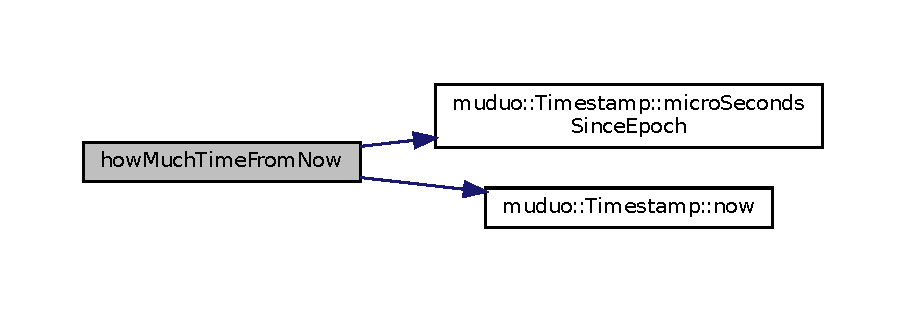
\includegraphics[width=350pt]{namespacemuduo_1_1detail_a14924335d79da967a69c650af3002c77_cgraph}
\end{center}
\end{figure}
这是这个函数的调用关系图\+:
\nopagebreak
\begin{figure}[H]
\begin{center}
\leavevmode
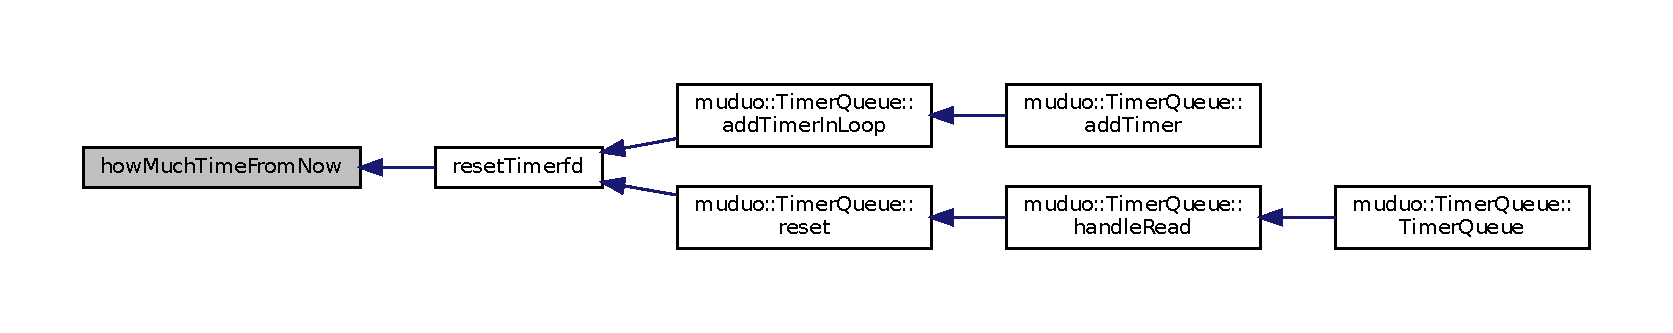
\includegraphics[width=350pt]{namespacemuduo_1_1detail_a14924335d79da967a69c650af3002c77_icgraph}
\end{center}
\end{figure}
\mbox{\Hypertarget{namespacemuduo_1_1detail_a08d79eafe298b7df1941adb4105bf75a}\label{namespacemuduo_1_1detail_a08d79eafe298b7df1941adb4105bf75a}} 
\index{muduo\+::detail@{muduo\+::detail}!read\+Timerfd@{read\+Timerfd}}
\index{read\+Timerfd@{read\+Timerfd}!muduo\+::detail@{muduo\+::detail}}
\subsubsection{\texorpdfstring{read\+Timerfd()}{readTimerfd()}}
{\footnotesize\ttfamily void muduo\+::detail\+::read\+Timerfd (\begin{DoxyParamCaption}\item[{int}]{timerfd,  }\item[{\hyperlink{classmuduo_1_1Timestamp}{Timestamp}}]{now }\end{DoxyParamCaption})}



在文件 Timer\+Queue.\+cc 第 37 行定义.



参考 L\+O\+G\+\_\+\+E\+R\+R\+OR, L\+O\+G\+\_\+\+T\+R\+A\+CE , 以及 Timestamp\+::to\+String().



参考自 Timer\+Queue\+::handle\+Read().

函数调用图\+:
\nopagebreak
\begin{figure}[H]
\begin{center}
\leavevmode
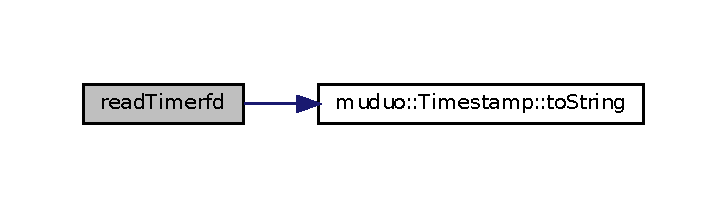
\includegraphics[width=349pt]{namespacemuduo_1_1detail_a08d79eafe298b7df1941adb4105bf75a_cgraph}
\end{center}
\end{figure}
这是这个函数的调用关系图\+:
\nopagebreak
\begin{figure}[H]
\begin{center}
\leavevmode
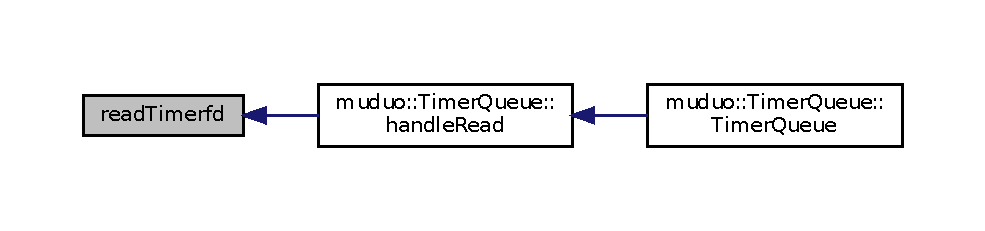
\includegraphics[width=350pt]{namespacemuduo_1_1detail_a08d79eafe298b7df1941adb4105bf75a_icgraph}
\end{center}
\end{figure}
\mbox{\Hypertarget{namespacemuduo_1_1detail_ae3e6bfc20f665df13eeb2ebc3c91abce}\label{namespacemuduo_1_1detail_ae3e6bfc20f665df13eeb2ebc3c91abce}} 
\index{muduo\+::detail@{muduo\+::detail}!remove\+Connection@{remove\+Connection}}
\index{remove\+Connection@{remove\+Connection}!muduo\+::detail@{muduo\+::detail}}
\subsubsection{\texorpdfstring{remove\+Connection()}{removeConnection()}}
{\footnotesize\ttfamily void muduo\+::detail\+::remove\+Connection (\begin{DoxyParamCaption}\item[{\hyperlink{classmuduo_1_1EventLoop}{Event\+Loop} $\ast$}]{loop,  }\item[{const \hyperlink{namespacemuduo_a40c45128e9700d337d92f3cbb8dd4a0a}{Tcp\+Connection\+Ptr} \&}]{conn }\end{DoxyParamCaption})}



在文件 Tcp\+Client.\+cc 第 19 行定义.



参考 Tcp\+Connection\+::connect\+Destoryed() , 以及 Event\+Loop\+::queue\+In\+Loop().



参考自 Tcp\+Client\+::$\sim$\+Tcp\+Client().

函数调用图\+:
\nopagebreak
\begin{figure}[H]
\begin{center}
\leavevmode
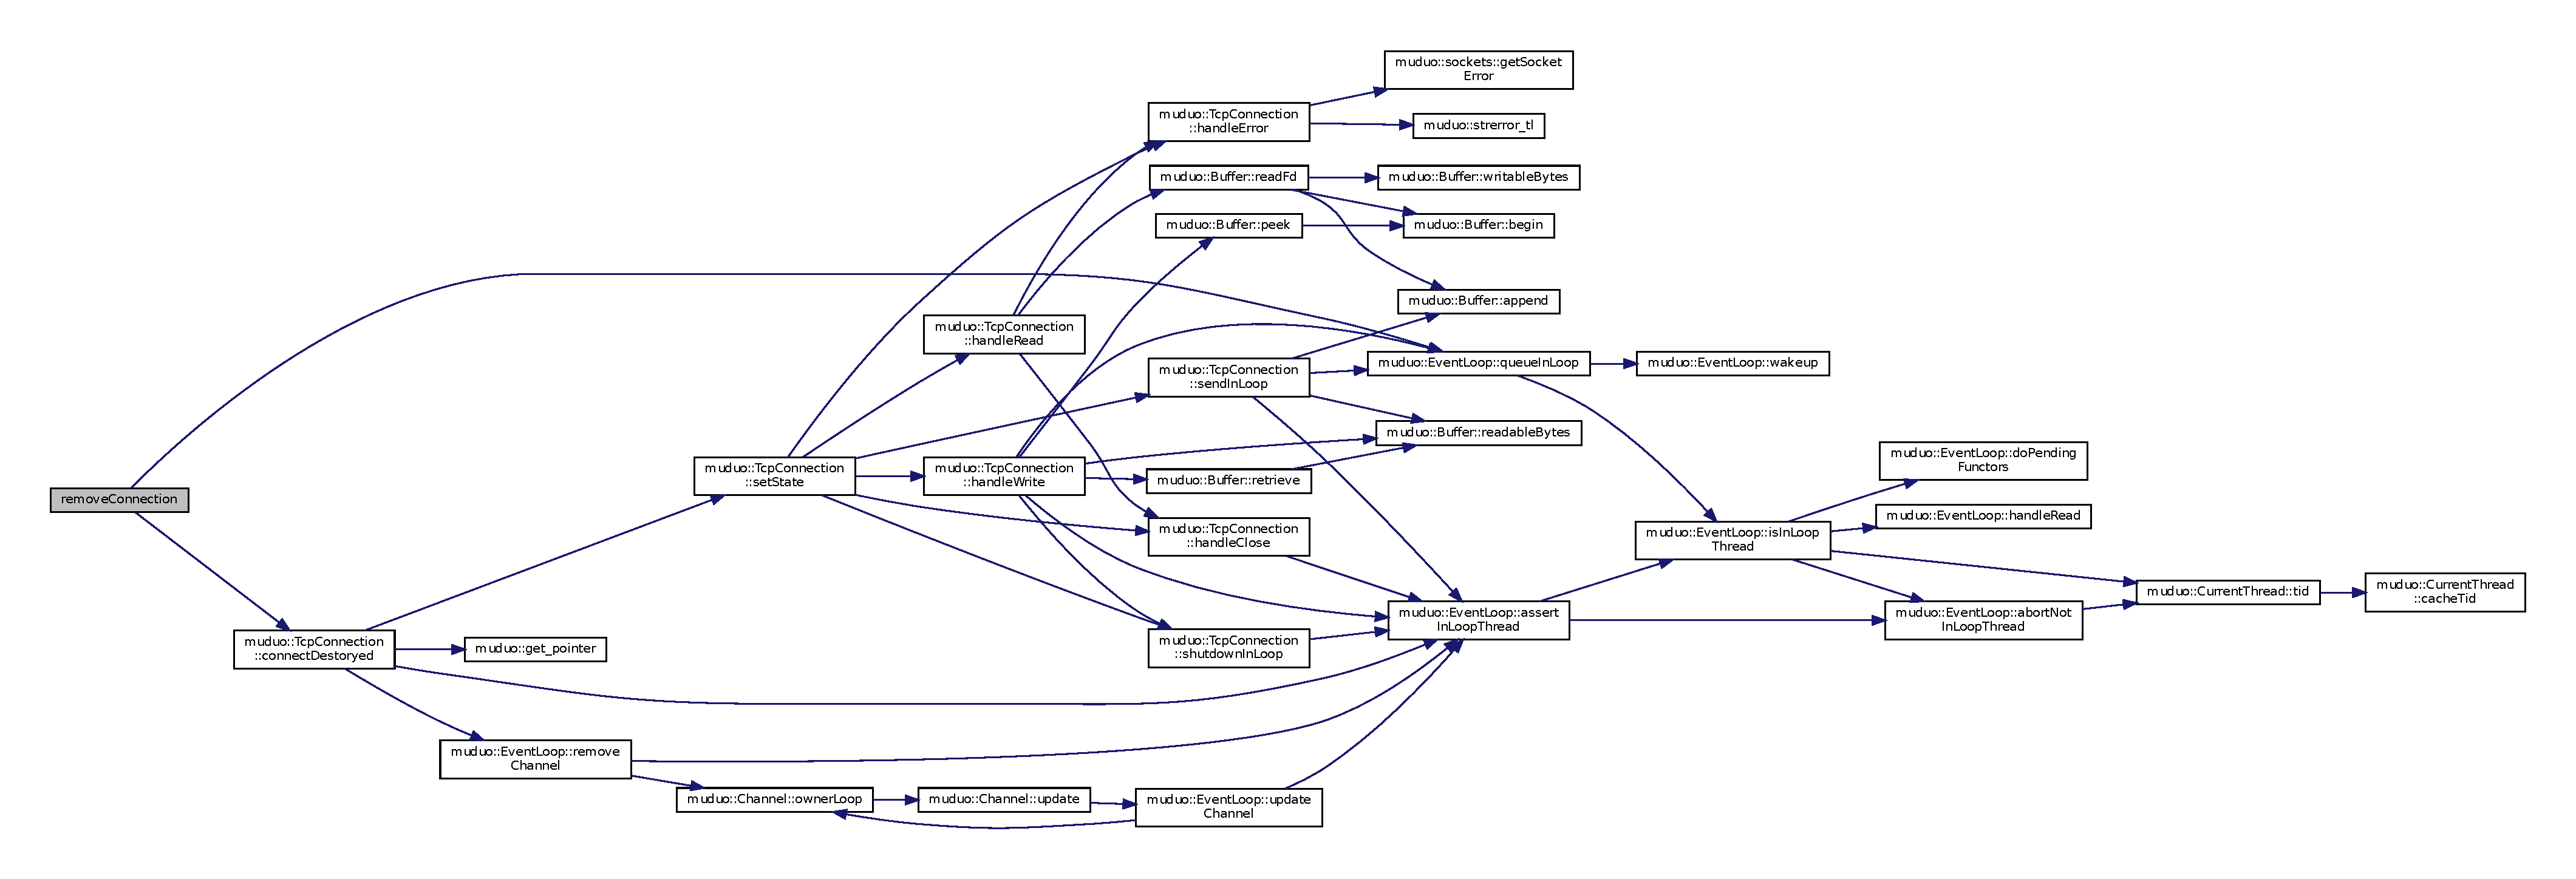
\includegraphics[width=350pt]{namespacemuduo_1_1detail_ae3e6bfc20f665df13eeb2ebc3c91abce_cgraph}
\end{center}
\end{figure}
这是这个函数的调用关系图\+:
\nopagebreak
\begin{figure}[H]
\begin{center}
\leavevmode
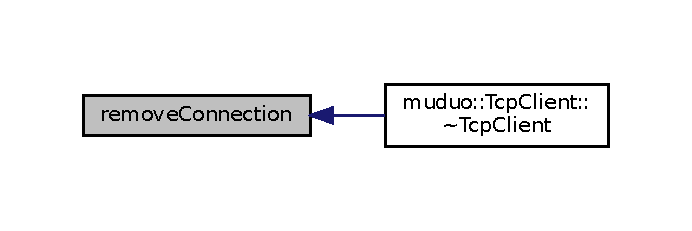
\includegraphics[width=332pt]{namespacemuduo_1_1detail_ae3e6bfc20f665df13eeb2ebc3c91abce_icgraph}
\end{center}
\end{figure}
\mbox{\Hypertarget{namespacemuduo_1_1detail_ab9f5e26fda4b27382acd5a0740a83137}\label{namespacemuduo_1_1detail_ab9f5e26fda4b27382acd5a0740a83137}} 
\index{muduo\+::detail@{muduo\+::detail}!remove\+Connector@{remove\+Connector}}
\index{remove\+Connector@{remove\+Connector}!muduo\+::detail@{muduo\+::detail}}
\subsubsection{\texorpdfstring{remove\+Connector()}{removeConnector()}}
{\footnotesize\ttfamily void muduo\+::detail\+::remove\+Connector (\begin{DoxyParamCaption}\item[{const \hyperlink{namespacemuduo_a144f8adea97b4c9ac75c439f6d87ae29}{Connector\+Ptr} \&}]{connector }\end{DoxyParamCaption})}



在文件 Tcp\+Client.\+cc 第 23 行定义.



参考自 Tcp\+Client\+::$\sim$\+Tcp\+Client().

这是这个函数的调用关系图\+:
\nopagebreak
\begin{figure}[H]
\begin{center}
\leavevmode
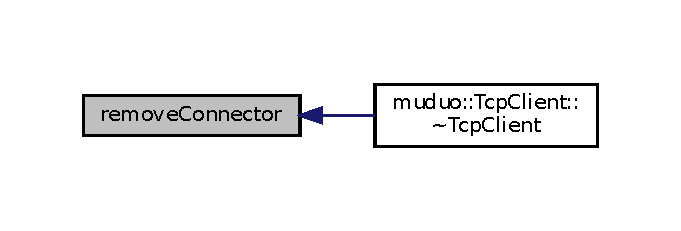
\includegraphics[width=327pt]{namespacemuduo_1_1detail_ab9f5e26fda4b27382acd5a0740a83137_icgraph}
\end{center}
\end{figure}
\mbox{\Hypertarget{namespacemuduo_1_1detail_a2a30bb501e8d9bb2da91ab353d1bc6fd}\label{namespacemuduo_1_1detail_a2a30bb501e8d9bb2da91ab353d1bc6fd}} 
\index{muduo\+::detail@{muduo\+::detail}!reset\+Timerfd@{reset\+Timerfd}}
\index{reset\+Timerfd@{reset\+Timerfd}!muduo\+::detail@{muduo\+::detail}}
\subsubsection{\texorpdfstring{reset\+Timerfd()}{resetTimerfd()}}
{\footnotesize\ttfamily void muduo\+::detail\+::reset\+Timerfd (\begin{DoxyParamCaption}\item[{int}]{timerfd,  }\item[{\hyperlink{classmuduo_1_1Timestamp}{Timestamp}}]{expiration }\end{DoxyParamCaption})}



在文件 Timer\+Queue.\+cc 第 46 行定义.



参考 how\+Much\+Time\+From\+Now() , 以及 L\+O\+G\+\_\+\+S\+Y\+S\+E\+RR.



参考自 Timer\+Queue\+::add\+Timer\+In\+Loop() , 以及 Timer\+Queue\+::reset().

函数调用图\+:
\nopagebreak
\begin{figure}[H]
\begin{center}
\leavevmode
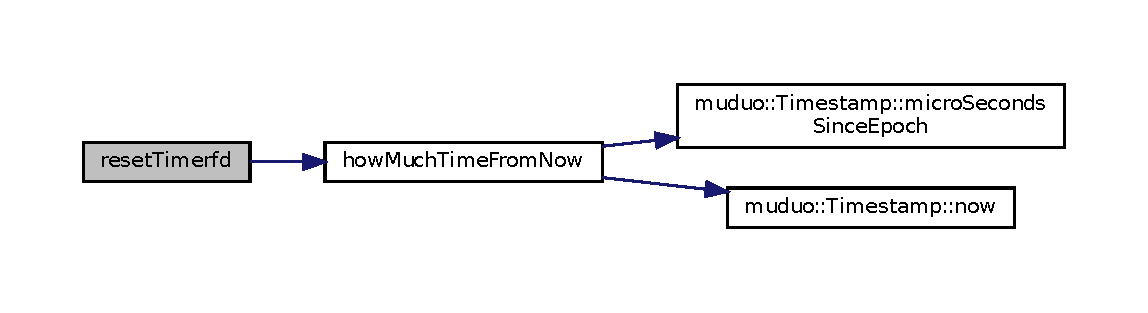
\includegraphics[width=350pt]{namespacemuduo_1_1detail_a2a30bb501e8d9bb2da91ab353d1bc6fd_cgraph}
\end{center}
\end{figure}
这是这个函数的调用关系图\+:
\nopagebreak
\begin{figure}[H]
\begin{center}
\leavevmode
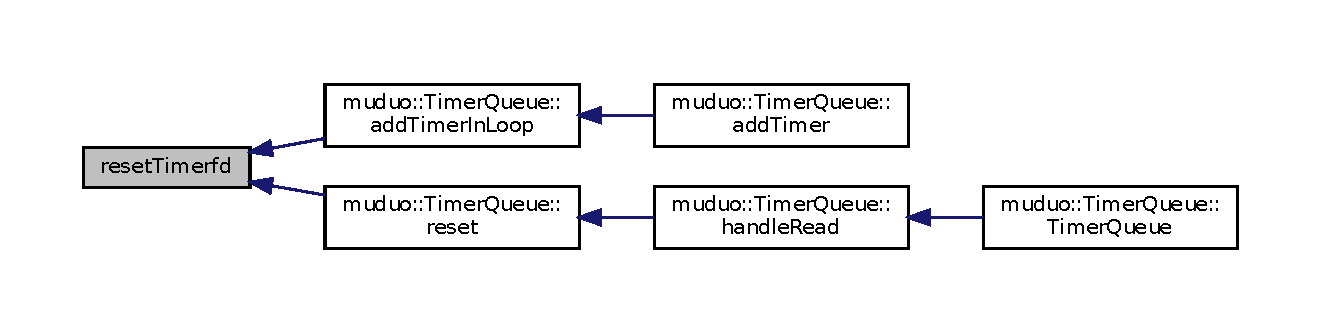
\includegraphics[width=350pt]{namespacemuduo_1_1detail_a2a30bb501e8d9bb2da91ab353d1bc6fd_icgraph}
\end{center}
\end{figure}


\subsection{变量说明}
\mbox{\Hypertarget{namespacemuduo_1_1detail_a72d89caa2e467f089bb6cc480d73b884}\label{namespacemuduo_1_1detail_a72d89caa2e467f089bb6cc480d73b884}} 
\index{muduo\+::detail@{muduo\+::detail}!k\+Large\+Buffer@{k\+Large\+Buffer}}
\index{k\+Large\+Buffer@{k\+Large\+Buffer}!muduo\+::detail@{muduo\+::detail}}
\subsubsection{\texorpdfstring{k\+Large\+Buffer}{kLargeBuffer}}
{\footnotesize\ttfamily const int k\+Large\+Buffer = 4000$\ast$1000}



在文件 Log\+Stream.\+h 第 22 行定义.

\mbox{\Hypertarget{namespacemuduo_1_1detail_a01441c3dba82e5d4bad1ce2b39ff576b}\label{namespacemuduo_1_1detail_a01441c3dba82e5d4bad1ce2b39ff576b}} 
\index{muduo\+::detail@{muduo\+::detail}!k\+Small\+Buffer@{k\+Small\+Buffer}}
\index{k\+Small\+Buffer@{k\+Small\+Buffer}!muduo\+::detail@{muduo\+::detail}}
\subsubsection{\texorpdfstring{k\+Small\+Buffer}{kSmallBuffer}}
{\footnotesize\ttfamily const int k\+Small\+Buffer = 4000}



在文件 Log\+Stream.\+h 第 21 行定义.


\hypertarget{namespacemuduo_1_1FileUtil}{}\section{muduo\+:\+:File\+Util 命名空间参考}
\label{namespacemuduo_1_1FileUtil}\index{muduo\+::\+File\+Util@{muduo\+::\+File\+Util}}
\subsection*{类}
\begin{DoxyCompactItemize}
\item 
class \hyperlink{classmuduo_1_1FileUtil_1_1AppendFile}{Append\+File}
\item 
class \hyperlink{classmuduo_1_1FileUtil_1_1ReadSmallFile}{Read\+Small\+File}
\end{DoxyCompactItemize}
\subsection*{函数}
\begin{DoxyCompactItemize}
\item 
{\footnotesize template$<$typename String $>$ }\\int \hyperlink{namespacemuduo_1_1FileUtil_a14a3368f5012ffe7b1004ef5b897fbbe}{read\+File} (\hyperlink{classmuduo_1_1StringArg}{String\+Arg} filename, int max\+Size, String $\ast$content, int64\+\_\+t $\ast$file\+Size=N\+U\+LL, int64\+\_\+t $\ast$modify\+Time=N\+U\+LL, int64\+\_\+t $\ast$create\+Time=N\+U\+LL)
\end{DoxyCompactItemize}


\subsection{函数说明}
\mbox{\Hypertarget{namespacemuduo_1_1FileUtil_a14a3368f5012ffe7b1004ef5b897fbbe}\label{namespacemuduo_1_1FileUtil_a14a3368f5012ffe7b1004ef5b897fbbe}} 
\index{muduo\+::\+File\+Util@{muduo\+::\+File\+Util}!read\+File@{read\+File}}
\index{read\+File@{read\+File}!muduo\+::\+File\+Util@{muduo\+::\+File\+Util}}
\subsubsection{\texorpdfstring{read\+File()}{readFile()}}
{\footnotesize\ttfamily int muduo\+::\+File\+Util\+::read\+File (\begin{DoxyParamCaption}\item[{\hyperlink{classmuduo_1_1StringArg}{String\+Arg}}]{filename,  }\item[{int}]{max\+Size,  }\item[{String $\ast$}]{content,  }\item[{int64\+\_\+t $\ast$}]{file\+Size = {\ttfamily NULL},  }\item[{int64\+\_\+t $\ast$}]{modify\+Time = {\ttfamily NULL},  }\item[{int64\+\_\+t $\ast$}]{create\+Time = {\ttfamily NULL} }\end{DoxyParamCaption})}



在文件 File\+Util.\+h 第 51 行定义.



参考 Read\+Small\+File\+::read\+To\+String().

函数调用图\+:
\nopagebreak
\begin{figure}[H]
\begin{center}
\leavevmode
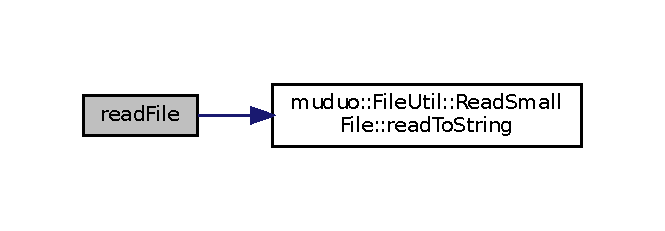
\includegraphics[width=319pt]{namespacemuduo_1_1FileUtil_a14a3368f5012ffe7b1004ef5b897fbbe_cgraph}
\end{center}
\end{figure}

\hypertarget{namespacemuduo_1_1net}{}\section{muduo\+:\+:net 命名空间参考}
\label{namespacemuduo_1_1net}\index{muduo\+::net@{muduo\+::net}}
\subsection*{命名空间}
\begin{DoxyCompactItemize}
\item 
 \hyperlink{namespacemuduo_1_1net_1_1sockets}{sockets}
\end{DoxyCompactItemize}
\subsection*{类}
\begin{DoxyCompactItemize}
\item 
class \hyperlink{classmuduo_1_1net_1_1Buffer}{Buffer}
\item 
class \hyperlink{classmuduo_1_1net_1_1Channel}{Channel}
\item 
class \hyperlink{classmuduo_1_1net_1_1EventLoop}{Event\+Loop}
\item 
class \hyperlink{classmuduo_1_1net_1_1EventLoopThread}{Event\+Loop\+Thread}
\item 
class \hyperlink{classmuduo_1_1net_1_1EventLoopThreadPool}{Event\+Loop\+Thread\+Pool}
\item 
class \hyperlink{classmuduo_1_1net_1_1HttpContext}{Http\+Context}
\item 
class \hyperlink{classmuduo_1_1net_1_1HttpRequest}{Http\+Request}
\item 
class \hyperlink{classmuduo_1_1net_1_1HttpResponse}{Http\+Response}
\item 
class \hyperlink{classmuduo_1_1net_1_1HttpServer}{Http\+Server}
\item 
class \hyperlink{classmuduo_1_1net_1_1InetAddress}{Inet\+Address}
\item 
class \hyperlink{classmuduo_1_1net_1_1Inspector}{Inspector}
\item 
class \hyperlink{classmuduo_1_1net_1_1PerformanceInspector}{Performance\+Inspector}
\item 
class \hyperlink{classmuduo_1_1net_1_1ProcessInspector}{Process\+Inspector}
\item 
class \hyperlink{classmuduo_1_1net_1_1SystemInspector}{System\+Inspector}
\item 
class \hyperlink{classmuduo_1_1net_1_1TcpClient}{Tcp\+Client}
\item 
class \hyperlink{classmuduo_1_1net_1_1TcpConnection}{Tcp\+Connection}
\item 
class \hyperlink{classmuduo_1_1net_1_1TcpServer}{Tcp\+Server}
\item 
class \hyperlink{classmuduo_1_1net_1_1TimerId}{Timer\+Id}
\end{DoxyCompactItemize}
\subsection*{类型定义}
\begin{DoxyCompactItemize}
\item 
typedef std\+::shared\+\_\+ptr$<$ \hyperlink{classmuduo_1_1net_1_1TcpConnection}{Tcp\+Connection} $>$ \hyperlink{namespacemuduo_1_1net_ab91a46e9290926aa692450e46cfc9039}{Tcp\+Connection\+Ptr}
\item 
typedef std\+::function$<$ void()$>$ \hyperlink{namespacemuduo_1_1net_ad4bd8788fd4c609b90c78920572bec50}{Timer\+Callback}
\item 
typedef std\+::function$<$ void(const \hyperlink{namespacemuduo_1_1net_ab91a46e9290926aa692450e46cfc9039}{Tcp\+Connection\+Ptr} \&)$>$ \hyperlink{namespacemuduo_1_1net_a78754792e997a13cb10908eb7ec508b2}{Connection\+Callback}
\item 
typedef std\+::function$<$ void(const \hyperlink{namespacemuduo_1_1net_ab91a46e9290926aa692450e46cfc9039}{Tcp\+Connection\+Ptr} \&)$>$ \hyperlink{namespacemuduo_1_1net_a5a393be65a093bad5f5a6b8340ce8c88}{Close\+Callback}
\item 
typedef std\+::function$<$ void(const \hyperlink{namespacemuduo_1_1net_ab91a46e9290926aa692450e46cfc9039}{Tcp\+Connection\+Ptr} \&)$>$ \hyperlink{namespacemuduo_1_1net_a525c3730bfefb763975b035ebc88a63d}{Write\+Complete\+Callback}
\item 
typedef std\+::function$<$ void(const \hyperlink{namespacemuduo_1_1net_ab91a46e9290926aa692450e46cfc9039}{Tcp\+Connection\+Ptr} \&, size\+\_\+t)$>$ \hyperlink{namespacemuduo_1_1net_a503c5e91d2e84874e83e9a6cbfb4a47b}{High\+Water\+Mark\+Callback}
\item 
typedef std\+::function$<$ void(const \hyperlink{namespacemuduo_1_1net_ab91a46e9290926aa692450e46cfc9039}{Tcp\+Connection\+Ptr} \&, \hyperlink{classmuduo_1_1net_1_1Buffer}{Buffer} $\ast$, \hyperlink{classmuduo_1_1Timestamp}{Timestamp})$>$ \hyperlink{namespacemuduo_1_1net_acaa802028467a41738aeb49699e85285}{Message\+Callback}
\item 
typedef std\+::shared\+\_\+ptr$<$ \hyperlink{classmuduo_1_1Connector}{Connector} $>$ \hyperlink{namespacemuduo_1_1net_adaac8e7754cfd0ac9c5a680eec411eba}{Connector\+Ptr}
\end{DoxyCompactItemize}
\subsection*{函数}
\begin{DoxyCompactItemize}
\item 
void \hyperlink{namespacemuduo_1_1net_a74d4cd57249902f889bfecb4bad7847d}{default\+Connection\+Callback} (const \hyperlink{namespacemuduo_1_1net_ab91a46e9290926aa692450e46cfc9039}{Tcp\+Connection\+Ptr} \&conn)
\item 
void \hyperlink{namespacemuduo_1_1net_abea01f500af8f956edd6649639937508}{default\+Message\+Callback} (const \hyperlink{namespacemuduo_1_1net_ab91a46e9290926aa692450e46cfc9039}{Tcp\+Connection\+Ptr} \&conn, \hyperlink{classmuduo_1_1net_1_1Buffer}{Buffer} $\ast$buffer, \hyperlink{classmuduo_1_1Timestamp}{Timestamp} receive\+Time)
\end{DoxyCompactItemize}


\subsection{类型定义说明}
\mbox{\Hypertarget{namespacemuduo_1_1net_a5a393be65a093bad5f5a6b8340ce8c88}\label{namespacemuduo_1_1net_a5a393be65a093bad5f5a6b8340ce8c88}} 
\index{muduo\+::net@{muduo\+::net}!Close\+Callback@{Close\+Callback}}
\index{Close\+Callback@{Close\+Callback}!muduo\+::net@{muduo\+::net}}
\subsubsection{\texorpdfstring{Close\+Callback}{CloseCallback}}
{\footnotesize\ttfamily typedef std\+::function$<$void (const \hyperlink{namespacemuduo_1_1net_ab91a46e9290926aa692450e46cfc9039}{Tcp\+Connection\+Ptr}\&)$>$ \hyperlink{namespacemuduo_1_1net_a5a393be65a093bad5f5a6b8340ce8c88}{Close\+Callback}}



在文件 Callbacks.\+h 第 65 行定义.

\mbox{\Hypertarget{namespacemuduo_1_1net_a78754792e997a13cb10908eb7ec508b2}\label{namespacemuduo_1_1net_a78754792e997a13cb10908eb7ec508b2}} 
\index{muduo\+::net@{muduo\+::net}!Connection\+Callback@{Connection\+Callback}}
\index{Connection\+Callback@{Connection\+Callback}!muduo\+::net@{muduo\+::net}}
\subsubsection{\texorpdfstring{Connection\+Callback}{ConnectionCallback}}
{\footnotesize\ttfamily typedef std\+::function$<$void (const \hyperlink{namespacemuduo_1_1net_ab91a46e9290926aa692450e46cfc9039}{Tcp\+Connection\+Ptr}\&)$>$ \hyperlink{namespacemuduo_1_1net_a78754792e997a13cb10908eb7ec508b2}{Connection\+Callback}}



在文件 Callbacks.\+h 第 64 行定义.

\mbox{\Hypertarget{namespacemuduo_1_1net_adaac8e7754cfd0ac9c5a680eec411eba}\label{namespacemuduo_1_1net_adaac8e7754cfd0ac9c5a680eec411eba}} 
\index{muduo\+::net@{muduo\+::net}!Connector\+Ptr@{Connector\+Ptr}}
\index{Connector\+Ptr@{Connector\+Ptr}!muduo\+::net@{muduo\+::net}}
\subsubsection{\texorpdfstring{Connector\+Ptr}{ConnectorPtr}}
{\footnotesize\ttfamily typedef std\+::shared\+\_\+ptr$<$\hyperlink{classmuduo_1_1Connector}{Connector}$>$ \hyperlink{namespacemuduo_1_1net_adaac8e7754cfd0ac9c5a680eec411eba}{Connector\+Ptr}}



在文件 Tcp\+Client.\+h 第 22 行定义.

\mbox{\Hypertarget{namespacemuduo_1_1net_a503c5e91d2e84874e83e9a6cbfb4a47b}\label{namespacemuduo_1_1net_a503c5e91d2e84874e83e9a6cbfb4a47b}} 
\index{muduo\+::net@{muduo\+::net}!High\+Water\+Mark\+Callback@{High\+Water\+Mark\+Callback}}
\index{High\+Water\+Mark\+Callback@{High\+Water\+Mark\+Callback}!muduo\+::net@{muduo\+::net}}
\subsubsection{\texorpdfstring{High\+Water\+Mark\+Callback}{HighWaterMarkCallback}}
{\footnotesize\ttfamily typedef std\+::function$<$void (const \hyperlink{namespacemuduo_1_1net_ab91a46e9290926aa692450e46cfc9039}{Tcp\+Connection\+Ptr}\&, size\+\_\+t)$>$ \hyperlink{namespacemuduo_1_1net_a503c5e91d2e84874e83e9a6cbfb4a47b}{High\+Water\+Mark\+Callback}}



在文件 Callbacks.\+h 第 67 行定义.

\mbox{\Hypertarget{namespacemuduo_1_1net_acaa802028467a41738aeb49699e85285}\label{namespacemuduo_1_1net_acaa802028467a41738aeb49699e85285}} 
\index{muduo\+::net@{muduo\+::net}!Message\+Callback@{Message\+Callback}}
\index{Message\+Callback@{Message\+Callback}!muduo\+::net@{muduo\+::net}}
\subsubsection{\texorpdfstring{Message\+Callback}{MessageCallback}}
{\footnotesize\ttfamily typedef std\+::function$<$void (const \hyperlink{namespacemuduo_1_1net_ab91a46e9290926aa692450e46cfc9039}{Tcp\+Connection\+Ptr}\&, \hyperlink{classmuduo_1_1net_1_1Buffer}{Buffer}$\ast$, \hyperlink{classmuduo_1_1Timestamp}{Timestamp})$>$ \hyperlink{namespacemuduo_1_1net_acaa802028467a41738aeb49699e85285}{Message\+Callback}}



在文件 Callbacks.\+h 第 72 行定义.

\mbox{\Hypertarget{namespacemuduo_1_1net_ab91a46e9290926aa692450e46cfc9039}\label{namespacemuduo_1_1net_ab91a46e9290926aa692450e46cfc9039}} 
\index{muduo\+::net@{muduo\+::net}!Tcp\+Connection\+Ptr@{Tcp\+Connection\+Ptr}}
\index{Tcp\+Connection\+Ptr@{Tcp\+Connection\+Ptr}!muduo\+::net@{muduo\+::net}}
\subsubsection{\texorpdfstring{Tcp\+Connection\+Ptr}{TcpConnectionPtr}}
{\footnotesize\ttfamily typedef std\+::shared\+\_\+ptr$<$ \hyperlink{classmuduo_1_1net_1_1TcpConnection}{Tcp\+Connection} $>$ \hyperlink{namespacemuduo_1_1net_ab91a46e9290926aa692450e46cfc9039}{Tcp\+Connection\+Ptr}}



在文件 Callbacks.\+h 第 61 行定义.

\mbox{\Hypertarget{namespacemuduo_1_1net_ad4bd8788fd4c609b90c78920572bec50}\label{namespacemuduo_1_1net_ad4bd8788fd4c609b90c78920572bec50}} 
\index{muduo\+::net@{muduo\+::net}!Timer\+Callback@{Timer\+Callback}}
\index{Timer\+Callback@{Timer\+Callback}!muduo\+::net@{muduo\+::net}}
\subsubsection{\texorpdfstring{Timer\+Callback}{TimerCallback}}
{\footnotesize\ttfamily typedef std\+::function$<$void()$>$ \hyperlink{namespacemuduo_1_1net_ad4bd8788fd4c609b90c78920572bec50}{Timer\+Callback}}



在文件 Callbacks.\+h 第 63 行定义.

\mbox{\Hypertarget{namespacemuduo_1_1net_a525c3730bfefb763975b035ebc88a63d}\label{namespacemuduo_1_1net_a525c3730bfefb763975b035ebc88a63d}} 
\index{muduo\+::net@{muduo\+::net}!Write\+Complete\+Callback@{Write\+Complete\+Callback}}
\index{Write\+Complete\+Callback@{Write\+Complete\+Callback}!muduo\+::net@{muduo\+::net}}
\subsubsection{\texorpdfstring{Write\+Complete\+Callback}{WriteCompleteCallback}}
{\footnotesize\ttfamily typedef std\+::function$<$void (const \hyperlink{namespacemuduo_1_1net_ab91a46e9290926aa692450e46cfc9039}{Tcp\+Connection\+Ptr}\&)$>$ \hyperlink{namespacemuduo_1_1net_a525c3730bfefb763975b035ebc88a63d}{Write\+Complete\+Callback}}



在文件 Callbacks.\+h 第 66 行定义.



\subsection{函数说明}
\mbox{\Hypertarget{namespacemuduo_1_1net_a74d4cd57249902f889bfecb4bad7847d}\label{namespacemuduo_1_1net_a74d4cd57249902f889bfecb4bad7847d}} 
\index{muduo\+::net@{muduo\+::net}!default\+Connection\+Callback@{default\+Connection\+Callback}}
\index{default\+Connection\+Callback@{default\+Connection\+Callback}!muduo\+::net@{muduo\+::net}}
\subsubsection{\texorpdfstring{default\+Connection\+Callback()}{defaultConnectionCallback()}}
{\footnotesize\ttfamily void muduo\+::net\+::default\+Connection\+Callback (\begin{DoxyParamCaption}\item[{const \hyperlink{namespacemuduo_1_1net_ab91a46e9290926aa692450e46cfc9039}{Tcp\+Connection\+Ptr} \&}]{conn }\end{DoxyParamCaption})}

\mbox{\Hypertarget{namespacemuduo_1_1net_abea01f500af8f956edd6649639937508}\label{namespacemuduo_1_1net_abea01f500af8f956edd6649639937508}} 
\index{muduo\+::net@{muduo\+::net}!default\+Message\+Callback@{default\+Message\+Callback}}
\index{default\+Message\+Callback@{default\+Message\+Callback}!muduo\+::net@{muduo\+::net}}
\subsubsection{\texorpdfstring{default\+Message\+Callback()}{defaultMessageCallback()}}
{\footnotesize\ttfamily void muduo\+::net\+::default\+Message\+Callback (\begin{DoxyParamCaption}\item[{const \hyperlink{namespacemuduo_1_1net_ab91a46e9290926aa692450e46cfc9039}{Tcp\+Connection\+Ptr} \&}]{conn,  }\item[{\hyperlink{classmuduo_1_1net_1_1Buffer}{Buffer} $\ast$}]{buffer,  }\item[{\hyperlink{classmuduo_1_1Timestamp}{Timestamp}}]{receive\+Time }\end{DoxyParamCaption})}


\hypertarget{namespacemuduo_1_1net_1_1sockets}{}\section{muduo\+:\+:net\+:\+:sockets 命名空间参考}
\label{namespacemuduo_1_1net_1_1sockets}\index{muduo\+::net\+::sockets@{muduo\+::net\+::sockets}}
\subsection*{函数}
\begin{DoxyCompactItemize}
\item 
uint64\+\_\+t \hyperlink{namespacemuduo_1_1net_1_1sockets_ad0a6476a5e70fb475acf4e34f5a5f8cc}{host\+To\+Network64} (uint64\+\_\+t host64)
\item 
uint32\+\_\+t \hyperlink{namespacemuduo_1_1net_1_1sockets_a4bb4a759c0f63477b89bac777f863cef}{host\+To\+Network32} (uint32\+\_\+t host32)
\item 
uint16\+\_\+t \hyperlink{namespacemuduo_1_1net_1_1sockets_ae117e4d96b27b387f167e75fb17c1834}{host\+To\+Network16} (uint16\+\_\+t host16)
\item 
uint64\+\_\+t \hyperlink{namespacemuduo_1_1net_1_1sockets_a590d67f0a8d4f8ff19462c08ebfb99b0}{network\+To\+Host64} (uint64\+\_\+t net64)
\item 
uint32\+\_\+t \hyperlink{namespacemuduo_1_1net_1_1sockets_a23f7d77e0379e52b1390e1d2846624e0}{network\+To\+Host32} (uint32\+\_\+t net32)
\item 
uint16\+\_\+t \hyperlink{namespacemuduo_1_1net_1_1sockets_a0f7768ebfa264d5c4eaf377297bab244}{network\+To\+Host16} (uint16\+\_\+t net16)
\item 
const struct sockaddr $\ast$ \hyperlink{namespacemuduo_1_1net_1_1sockets_ad69bf980a58ef6798c4e1dbe5497d52c}{sockaddr\+\_\+cast} (const struct sockaddr\+\_\+in6 $\ast$addr)
\end{DoxyCompactItemize}


\subsection{函数说明}
\mbox{\Hypertarget{namespacemuduo_1_1net_1_1sockets_ae117e4d96b27b387f167e75fb17c1834}\label{namespacemuduo_1_1net_1_1sockets_ae117e4d96b27b387f167e75fb17c1834}} 
\index{muduo\+::net\+::sockets@{muduo\+::net\+::sockets}!host\+To\+Network16@{host\+To\+Network16}}
\index{host\+To\+Network16@{host\+To\+Network16}!muduo\+::net\+::sockets@{muduo\+::net\+::sockets}}
\subsubsection{\texorpdfstring{host\+To\+Network16()}{hostToNetwork16()}}
{\footnotesize\ttfamily uint16\+\_\+t muduo\+::net\+::sockets\+::host\+To\+Network16 (\begin{DoxyParamCaption}\item[{uint16\+\_\+t}]{host16 }\end{DoxyParamCaption})\hspace{0.3cm}{\ttfamily [inline]}}



在文件 Endian.\+h 第 39 行定义.



参考自 Buffer\+::append\+Int16(), muduo\+::sockets\+::from\+Host\+Port() , 以及 Buffer\+::prepend\+Int16().

这是这个函数的调用关系图\+:
\nopagebreak
\begin{figure}[H]
\begin{center}
\leavevmode
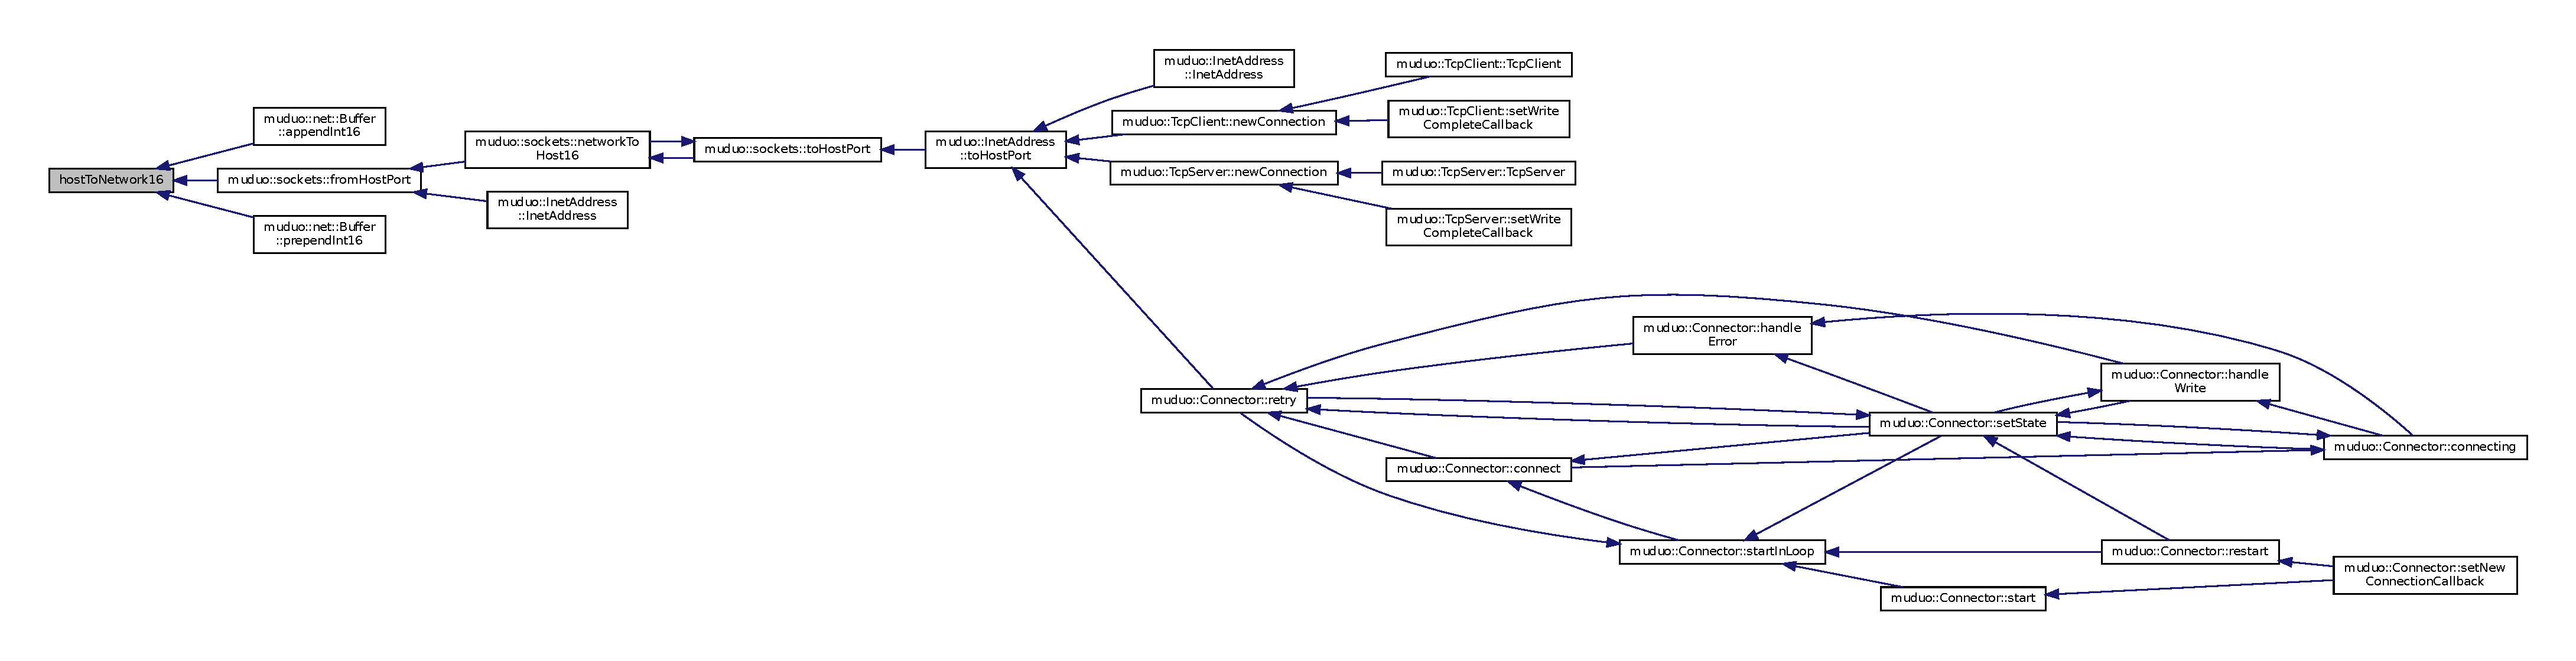
\includegraphics[width=350pt]{namespacemuduo_1_1net_1_1sockets_ae117e4d96b27b387f167e75fb17c1834_icgraph}
\end{center}
\end{figure}
\mbox{\Hypertarget{namespacemuduo_1_1net_1_1sockets_a4bb4a759c0f63477b89bac777f863cef}\label{namespacemuduo_1_1net_1_1sockets_a4bb4a759c0f63477b89bac777f863cef}} 
\index{muduo\+::net\+::sockets@{muduo\+::net\+::sockets}!host\+To\+Network32@{host\+To\+Network32}}
\index{host\+To\+Network32@{host\+To\+Network32}!muduo\+::net\+::sockets@{muduo\+::net\+::sockets}}
\subsubsection{\texorpdfstring{host\+To\+Network32()}{hostToNetwork32()}}
{\footnotesize\ttfamily uint32\+\_\+t muduo\+::net\+::sockets\+::host\+To\+Network32 (\begin{DoxyParamCaption}\item[{uint32\+\_\+t}]{host32 }\end{DoxyParamCaption})\hspace{0.3cm}{\ttfamily [inline]}}



在文件 Endian.\+h 第 34 行定义.



参考自 Buffer\+::append\+Int32() , 以及 Buffer\+::prepend\+Int32().

这是这个函数的调用关系图\+:
\nopagebreak
\begin{figure}[H]
\begin{center}
\leavevmode
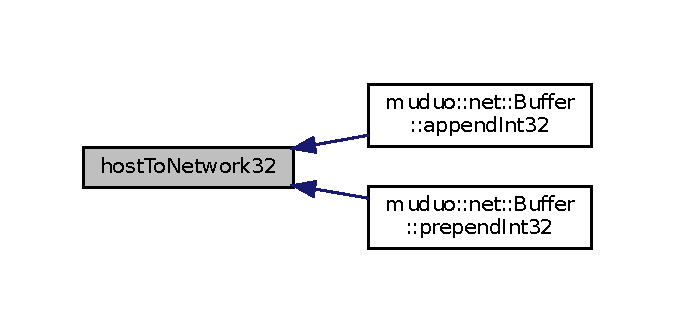
\includegraphics[width=324pt]{namespacemuduo_1_1net_1_1sockets_a4bb4a759c0f63477b89bac777f863cef_icgraph}
\end{center}
\end{figure}
\mbox{\Hypertarget{namespacemuduo_1_1net_1_1sockets_ad0a6476a5e70fb475acf4e34f5a5f8cc}\label{namespacemuduo_1_1net_1_1sockets_ad0a6476a5e70fb475acf4e34f5a5f8cc}} 
\index{muduo\+::net\+::sockets@{muduo\+::net\+::sockets}!host\+To\+Network64@{host\+To\+Network64}}
\index{host\+To\+Network64@{host\+To\+Network64}!muduo\+::net\+::sockets@{muduo\+::net\+::sockets}}
\subsubsection{\texorpdfstring{host\+To\+Network64()}{hostToNetwork64()}}
{\footnotesize\ttfamily uint64\+\_\+t muduo\+::net\+::sockets\+::host\+To\+Network64 (\begin{DoxyParamCaption}\item[{uint64\+\_\+t}]{host64 }\end{DoxyParamCaption})\hspace{0.3cm}{\ttfamily [inline]}}



在文件 Endian.\+h 第 29 行定义.



参考自 Buffer\+::append\+Int64() , 以及 Buffer\+::prepend\+Int64().

这是这个函数的调用关系图\+:
\nopagebreak
\begin{figure}[H]
\begin{center}
\leavevmode
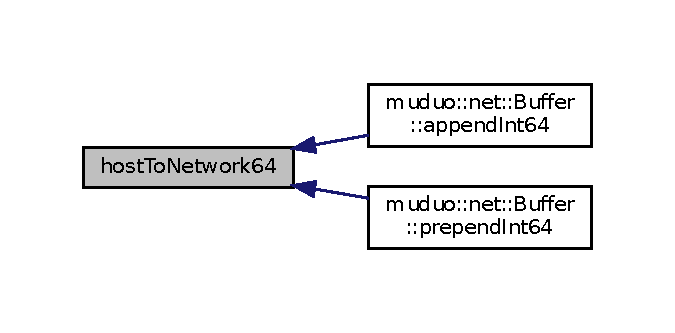
\includegraphics[width=324pt]{namespacemuduo_1_1net_1_1sockets_ad0a6476a5e70fb475acf4e34f5a5f8cc_icgraph}
\end{center}
\end{figure}
\mbox{\Hypertarget{namespacemuduo_1_1net_1_1sockets_a0f7768ebfa264d5c4eaf377297bab244}\label{namespacemuduo_1_1net_1_1sockets_a0f7768ebfa264d5c4eaf377297bab244}} 
\index{muduo\+::net\+::sockets@{muduo\+::net\+::sockets}!network\+To\+Host16@{network\+To\+Host16}}
\index{network\+To\+Host16@{network\+To\+Host16}!muduo\+::net\+::sockets@{muduo\+::net\+::sockets}}
\subsubsection{\texorpdfstring{network\+To\+Host16()}{networkToHost16()}}
{\footnotesize\ttfamily uint16\+\_\+t muduo\+::net\+::sockets\+::network\+To\+Host16 (\begin{DoxyParamCaption}\item[{uint16\+\_\+t}]{net16 }\end{DoxyParamCaption})\hspace{0.3cm}{\ttfamily [inline]}}



在文件 Endian.\+h 第 54 行定义.



参考自 Buffer\+::peek\+Int16().

这是这个函数的调用关系图\+:
\nopagebreak
\begin{figure}[H]
\begin{center}
\leavevmode
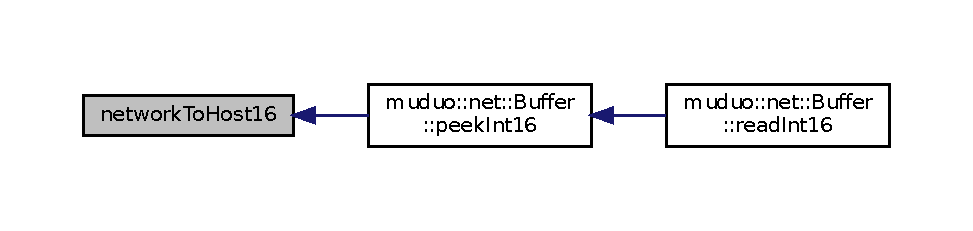
\includegraphics[width=350pt]{namespacemuduo_1_1net_1_1sockets_a0f7768ebfa264d5c4eaf377297bab244_icgraph}
\end{center}
\end{figure}
\mbox{\Hypertarget{namespacemuduo_1_1net_1_1sockets_a23f7d77e0379e52b1390e1d2846624e0}\label{namespacemuduo_1_1net_1_1sockets_a23f7d77e0379e52b1390e1d2846624e0}} 
\index{muduo\+::net\+::sockets@{muduo\+::net\+::sockets}!network\+To\+Host32@{network\+To\+Host32}}
\index{network\+To\+Host32@{network\+To\+Host32}!muduo\+::net\+::sockets@{muduo\+::net\+::sockets}}
\subsubsection{\texorpdfstring{network\+To\+Host32()}{networkToHost32()}}
{\footnotesize\ttfamily uint32\+\_\+t muduo\+::net\+::sockets\+::network\+To\+Host32 (\begin{DoxyParamCaption}\item[{uint32\+\_\+t}]{net32 }\end{DoxyParamCaption})\hspace{0.3cm}{\ttfamily [inline]}}



在文件 Endian.\+h 第 49 行定义.



参考自 Buffer\+::peek\+Int32().

这是这个函数的调用关系图\+:
\nopagebreak
\begin{figure}[H]
\begin{center}
\leavevmode
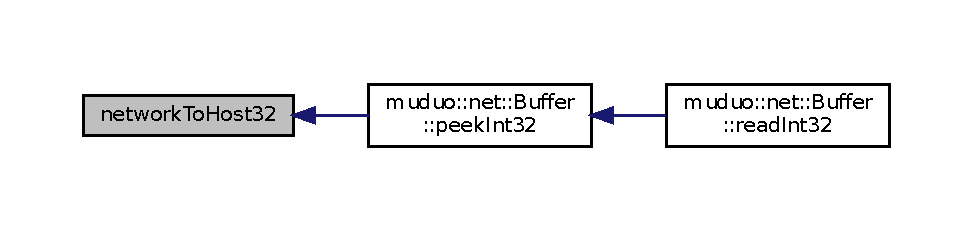
\includegraphics[width=350pt]{namespacemuduo_1_1net_1_1sockets_a23f7d77e0379e52b1390e1d2846624e0_icgraph}
\end{center}
\end{figure}
\mbox{\Hypertarget{namespacemuduo_1_1net_1_1sockets_a590d67f0a8d4f8ff19462c08ebfb99b0}\label{namespacemuduo_1_1net_1_1sockets_a590d67f0a8d4f8ff19462c08ebfb99b0}} 
\index{muduo\+::net\+::sockets@{muduo\+::net\+::sockets}!network\+To\+Host64@{network\+To\+Host64}}
\index{network\+To\+Host64@{network\+To\+Host64}!muduo\+::net\+::sockets@{muduo\+::net\+::sockets}}
\subsubsection{\texorpdfstring{network\+To\+Host64()}{networkToHost64()}}
{\footnotesize\ttfamily uint64\+\_\+t muduo\+::net\+::sockets\+::network\+To\+Host64 (\begin{DoxyParamCaption}\item[{uint64\+\_\+t}]{net64 }\end{DoxyParamCaption})\hspace{0.3cm}{\ttfamily [inline]}}



在文件 Endian.\+h 第 44 行定义.



参考自 Buffer\+::peek\+Int64().

这是这个函数的调用关系图\+:
\nopagebreak
\begin{figure}[H]
\begin{center}
\leavevmode
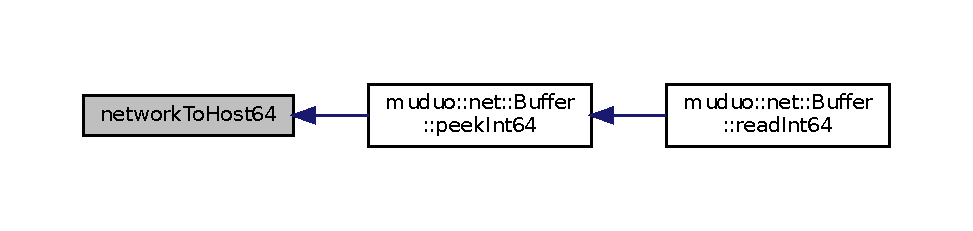
\includegraphics[width=350pt]{namespacemuduo_1_1net_1_1sockets_a590d67f0a8d4f8ff19462c08ebfb99b0_icgraph}
\end{center}
\end{figure}
\mbox{\Hypertarget{namespacemuduo_1_1net_1_1sockets_ad69bf980a58ef6798c4e1dbe5497d52c}\label{namespacemuduo_1_1net_1_1sockets_ad69bf980a58ef6798c4e1dbe5497d52c}} 
\index{muduo\+::net\+::sockets@{muduo\+::net\+::sockets}!sockaddr\+\_\+cast@{sockaddr\+\_\+cast}}
\index{sockaddr\+\_\+cast@{sockaddr\+\_\+cast}!muduo\+::net\+::sockets@{muduo\+::net\+::sockets}}
\subsubsection{\texorpdfstring{sockaddr\+\_\+cast()}{sockaddr\_cast()}}
{\footnotesize\ttfamily const struct sockaddr$\ast$ muduo\+::net\+::sockets\+::sockaddr\+\_\+cast (\begin{DoxyParamCaption}\item[{const struct sockaddr\+\_\+in6 $\ast$}]{addr }\end{DoxyParamCaption})}



参考自 muduo\+::sockets\+::accept(), muduo\+::sockets\+::bind\+Or\+Die(), muduo\+::sockets\+::connect(), muduo\+::sockets\+::get\+Local\+Addr(), muduo\+::sockets\+::get\+Peer\+Addr() , 以及 Inet\+Address\+::get\+Sock\+Addr().

这是这个函数的调用关系图\+:
\nopagebreak
\begin{figure}[H]
\begin{center}
\leavevmode
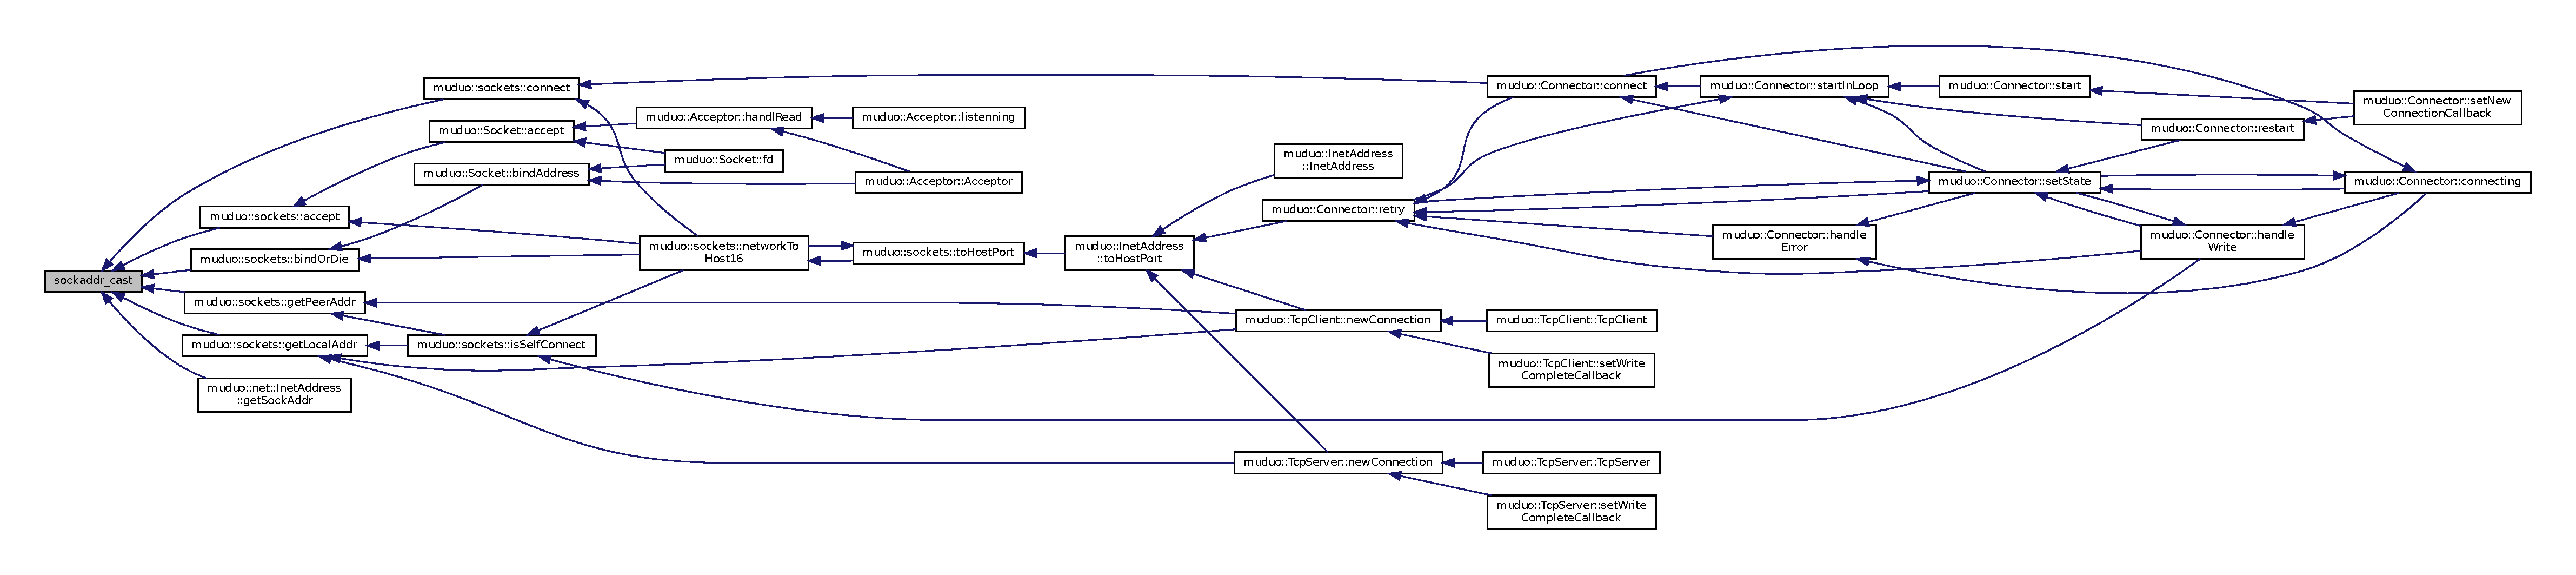
\includegraphics[width=350pt]{namespacemuduo_1_1net_1_1sockets_ad69bf980a58ef6798c4e1dbe5497d52c_icgraph}
\end{center}
\end{figure}

\hypertarget{namespacemuduo_1_1ProcessInfo}{}\section{muduo\+:\+:Process\+Info 命名空间参考}
\label{namespacemuduo_1_1ProcessInfo}\index{muduo\+::\+Process\+Info@{muduo\+::\+Process\+Info}}
\subsection*{类}
\begin{DoxyCompactItemize}
\item 
struct \hyperlink{structmuduo_1_1ProcessInfo_1_1CpuTime}{Cpu\+Time}
\end{DoxyCompactItemize}
\subsection*{函数}
\begin{DoxyCompactItemize}
\item 
pid\+\_\+t \hyperlink{namespacemuduo_1_1ProcessInfo_a9b565d9cb6c35649f0feeeaa8b26dd7b}{pid} ()
\item 
string \hyperlink{namespacemuduo_1_1ProcessInfo_af54b6cc2e94622bf45a9ced0093b7dae}{pid\+String} ()
\item 
uid\+\_\+t \hyperlink{namespacemuduo_1_1ProcessInfo_a056245f62bbe6e8abdcd42171a432aac}{uid} ()
\item 
string \hyperlink{namespacemuduo_1_1ProcessInfo_a54e6907a19c94da2cf5db8dcad530262}{username} ()
\item 
uid\+\_\+t \hyperlink{namespacemuduo_1_1ProcessInfo_a7313897d7ec7dc5bbdd8f3f88c449b7e}{euid} ()
\item 
\hyperlink{classmuduo_1_1Timestamp}{Timestamp} \hyperlink{namespacemuduo_1_1ProcessInfo_a3662fa984eef69a557c6d997aba58e18}{start\+Time} ()
\item 
int \hyperlink{namespacemuduo_1_1ProcessInfo_af8d3ce061f87c1a208c8e164e9b69882}{clock\+Ticks\+Per\+Second} ()
\item 
int \hyperlink{namespacemuduo_1_1ProcessInfo_a3aab01e3a27d7f88b7d8fffceb529c64}{page\+Size} ()
\item 
bool \hyperlink{namespacemuduo_1_1ProcessInfo_aabe41272bf5623d260fe92399071ed4e}{is\+Debug\+Build} ()
\item 
string \hyperlink{namespacemuduo_1_1ProcessInfo_ac60f3a33a07318aa231cc3d07f6ee419}{hostname} ()
\item 
string \hyperlink{namespacemuduo_1_1ProcessInfo_ac8a6ab8cb6657fc7ddba4a8be2f60e2b}{procname} ()
\item 
\hyperlink{classmuduo_1_1StringPiece}{String\+Piece} \hyperlink{namespacemuduo_1_1ProcessInfo_acb222d923a768bc8e9ecceaf21ac4ba3}{procname} (const string \&stat)
\item 
string \hyperlink{namespacemuduo_1_1ProcessInfo_a930c5a6d17d6ba40f7011643f4442c41}{proc\+Status} ()
\begin{DoxyCompactList}\small\item\em read /proc/self/status \end{DoxyCompactList}\item 
string \hyperlink{namespacemuduo_1_1ProcessInfo_a8f557f94d9b8cdb55a8d21c5b6c70634}{proc\+Stat} ()
\begin{DoxyCompactList}\small\item\em read /proc/self/stat \end{DoxyCompactList}\item 
string \hyperlink{namespacemuduo_1_1ProcessInfo_a7d3faa2d63f4cf7b8ba073a3daf7ffb1}{thread\+Stat} ()
\begin{DoxyCompactList}\small\item\em read /proc/self/task/tid/stat \end{DoxyCompactList}\item 
string \hyperlink{namespacemuduo_1_1ProcessInfo_acdf231e7f033258ea9e93f1a4d651c50}{exe\+Path} ()
\begin{DoxyCompactList}\small\item\em readlink /proc/self/exe \end{DoxyCompactList}\item 
int \hyperlink{namespacemuduo_1_1ProcessInfo_aa8e6192d04097a3864d8c07bf24e4ff9}{opened\+Files} ()
\item 
int \hyperlink{namespacemuduo_1_1ProcessInfo_a2bb52b7cbab50f7bc977048005845c67}{max\+Open\+Files} ()
\item 
\hyperlink{structmuduo_1_1ProcessInfo_1_1CpuTime}{Cpu\+Time} \hyperlink{namespacemuduo_1_1ProcessInfo_a0e67cc8ad47ff86331b6d2a509d14648}{cpu\+Time} ()
\item 
int \hyperlink{namespacemuduo_1_1ProcessInfo_a120db223841da7c65566c1fb2a06befa}{num\+Threads} ()
\item 
std\+::vector$<$ pid\+\_\+t $>$ \hyperlink{namespacemuduo_1_1ProcessInfo_a360aafb2759971d7c8190b1a60f7dc03}{threads} ()
\end{DoxyCompactItemize}


\subsection{函数说明}
\mbox{\Hypertarget{namespacemuduo_1_1ProcessInfo_af8d3ce061f87c1a208c8e164e9b69882}\label{namespacemuduo_1_1ProcessInfo_af8d3ce061f87c1a208c8e164e9b69882}} 
\index{muduo\+::\+Process\+Info@{muduo\+::\+Process\+Info}!clock\+Ticks\+Per\+Second@{clock\+Ticks\+Per\+Second}}
\index{clock\+Ticks\+Per\+Second@{clock\+Ticks\+Per\+Second}!muduo\+::\+Process\+Info@{muduo\+::\+Process\+Info}}
\subsubsection{\texorpdfstring{clock\+Ticks\+Per\+Second()}{clockTicksPerSecond()}}
{\footnotesize\ttfamily int muduo\+::\+Process\+Info\+::clock\+Ticks\+Per\+Second (\begin{DoxyParamCaption}{ }\end{DoxyParamCaption})}

\mbox{\Hypertarget{namespacemuduo_1_1ProcessInfo_a0e67cc8ad47ff86331b6d2a509d14648}\label{namespacemuduo_1_1ProcessInfo_a0e67cc8ad47ff86331b6d2a509d14648}} 
\index{muduo\+::\+Process\+Info@{muduo\+::\+Process\+Info}!cpu\+Time@{cpu\+Time}}
\index{cpu\+Time@{cpu\+Time}!muduo\+::\+Process\+Info@{muduo\+::\+Process\+Info}}
\subsubsection{\texorpdfstring{cpu\+Time()}{cpuTime()}}
{\footnotesize\ttfamily \hyperlink{structmuduo_1_1ProcessInfo_1_1CpuTime}{Cpu\+Time} muduo\+::\+Process\+Info\+::cpu\+Time (\begin{DoxyParamCaption}{ }\end{DoxyParamCaption})}



参考自 Cpu\+Time\+::total().

这是这个函数的调用关系图\+:
\nopagebreak
\begin{figure}[H]
\begin{center}
\leavevmode
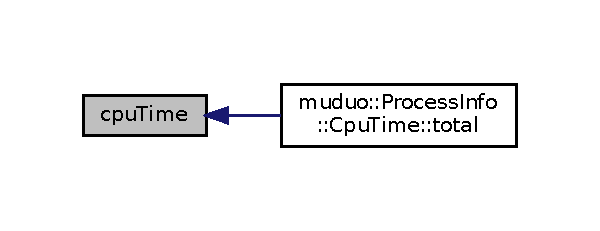
\includegraphics[width=288pt]{namespacemuduo_1_1ProcessInfo_a0e67cc8ad47ff86331b6d2a509d14648_icgraph}
\end{center}
\end{figure}
\mbox{\Hypertarget{namespacemuduo_1_1ProcessInfo_a7313897d7ec7dc5bbdd8f3f88c449b7e}\label{namespacemuduo_1_1ProcessInfo_a7313897d7ec7dc5bbdd8f3f88c449b7e}} 
\index{muduo\+::\+Process\+Info@{muduo\+::\+Process\+Info}!euid@{euid}}
\index{euid@{euid}!muduo\+::\+Process\+Info@{muduo\+::\+Process\+Info}}
\subsubsection{\texorpdfstring{euid()}{euid()}}
{\footnotesize\ttfamily uid\+\_\+t muduo\+::\+Process\+Info\+::euid (\begin{DoxyParamCaption}{ }\end{DoxyParamCaption})}

\mbox{\Hypertarget{namespacemuduo_1_1ProcessInfo_acdf231e7f033258ea9e93f1a4d651c50}\label{namespacemuduo_1_1ProcessInfo_acdf231e7f033258ea9e93f1a4d651c50}} 
\index{muduo\+::\+Process\+Info@{muduo\+::\+Process\+Info}!exe\+Path@{exe\+Path}}
\index{exe\+Path@{exe\+Path}!muduo\+::\+Process\+Info@{muduo\+::\+Process\+Info}}
\subsubsection{\texorpdfstring{exe\+Path()}{exePath()}}
{\footnotesize\ttfamily string muduo\+::\+Process\+Info\+::exe\+Path (\begin{DoxyParamCaption}{ }\end{DoxyParamCaption})}



readlink /proc/self/exe 

\mbox{\Hypertarget{namespacemuduo_1_1ProcessInfo_ac60f3a33a07318aa231cc3d07f6ee419}\label{namespacemuduo_1_1ProcessInfo_ac60f3a33a07318aa231cc3d07f6ee419}} 
\index{muduo\+::\+Process\+Info@{muduo\+::\+Process\+Info}!hostname@{hostname}}
\index{hostname@{hostname}!muduo\+::\+Process\+Info@{muduo\+::\+Process\+Info}}
\subsubsection{\texorpdfstring{hostname()}{hostname()}}
{\footnotesize\ttfamily string muduo\+::\+Process\+Info\+::hostname (\begin{DoxyParamCaption}{ }\end{DoxyParamCaption})}



参考自 Inet\+Address\+::port\+Net\+Endian().

这是这个函数的调用关系图\+:
\nopagebreak
\begin{figure}[H]
\begin{center}
\leavevmode
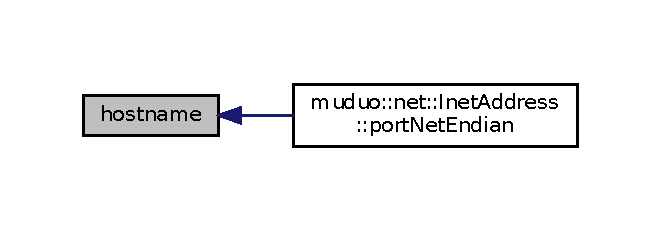
\includegraphics[width=317pt]{namespacemuduo_1_1ProcessInfo_ac60f3a33a07318aa231cc3d07f6ee419_icgraph}
\end{center}
\end{figure}
\mbox{\Hypertarget{namespacemuduo_1_1ProcessInfo_aabe41272bf5623d260fe92399071ed4e}\label{namespacemuduo_1_1ProcessInfo_aabe41272bf5623d260fe92399071ed4e}} 
\index{muduo\+::\+Process\+Info@{muduo\+::\+Process\+Info}!is\+Debug\+Build@{is\+Debug\+Build}}
\index{is\+Debug\+Build@{is\+Debug\+Build}!muduo\+::\+Process\+Info@{muduo\+::\+Process\+Info}}
\subsubsection{\texorpdfstring{is\+Debug\+Build()}{isDebugBuild()}}
{\footnotesize\ttfamily bool muduo\+::\+Process\+Info\+::is\+Debug\+Build (\begin{DoxyParamCaption}{ }\end{DoxyParamCaption})}

\mbox{\Hypertarget{namespacemuduo_1_1ProcessInfo_a2bb52b7cbab50f7bc977048005845c67}\label{namespacemuduo_1_1ProcessInfo_a2bb52b7cbab50f7bc977048005845c67}} 
\index{muduo\+::\+Process\+Info@{muduo\+::\+Process\+Info}!max\+Open\+Files@{max\+Open\+Files}}
\index{max\+Open\+Files@{max\+Open\+Files}!muduo\+::\+Process\+Info@{muduo\+::\+Process\+Info}}
\subsubsection{\texorpdfstring{max\+Open\+Files()}{maxOpenFiles()}}
{\footnotesize\ttfamily int muduo\+::\+Process\+Info\+::max\+Open\+Files (\begin{DoxyParamCaption}{ }\end{DoxyParamCaption})}

\mbox{\Hypertarget{namespacemuduo_1_1ProcessInfo_a120db223841da7c65566c1fb2a06befa}\label{namespacemuduo_1_1ProcessInfo_a120db223841da7c65566c1fb2a06befa}} 
\index{muduo\+::\+Process\+Info@{muduo\+::\+Process\+Info}!num\+Threads@{num\+Threads}}
\index{num\+Threads@{num\+Threads}!muduo\+::\+Process\+Info@{muduo\+::\+Process\+Info}}
\subsubsection{\texorpdfstring{num\+Threads()}{numThreads()}}
{\footnotesize\ttfamily int muduo\+::\+Process\+Info\+::num\+Threads (\begin{DoxyParamCaption}{ }\end{DoxyParamCaption})}



参考自 Tcp\+Server\+::get\+Loop(), Thread\+Pool\+::set\+Thread\+Init\+Callback(), Event\+Loop\+Thread\+Pool\+::set\+Thread\+Num() , 以及 Cpu\+Time\+::total().

这是这个函数的调用关系图\+:
\nopagebreak
\begin{figure}[H]
\begin{center}
\leavevmode
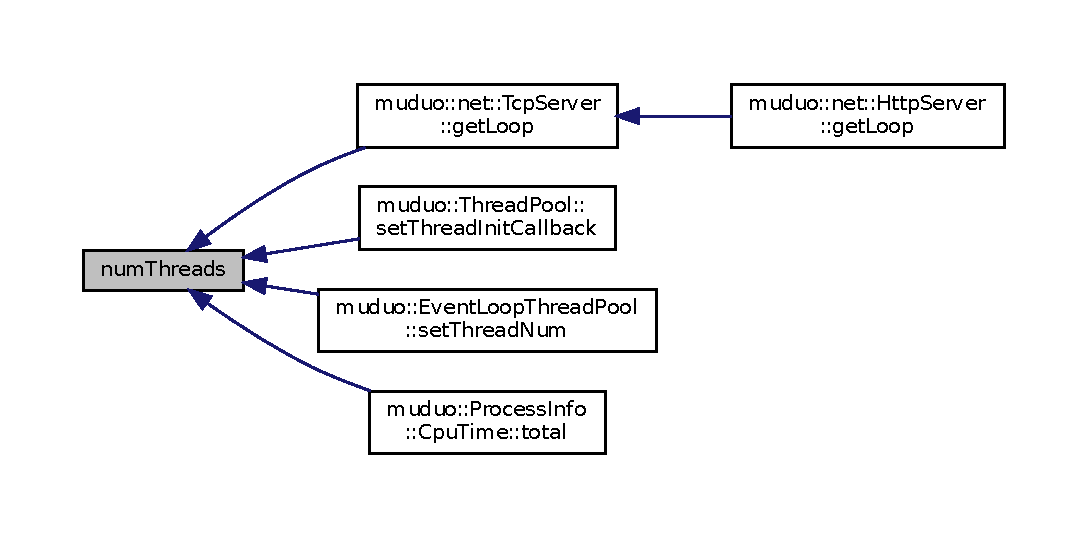
\includegraphics[width=350pt]{namespacemuduo_1_1ProcessInfo_a120db223841da7c65566c1fb2a06befa_icgraph}
\end{center}
\end{figure}
\mbox{\Hypertarget{namespacemuduo_1_1ProcessInfo_aa8e6192d04097a3864d8c07bf24e4ff9}\label{namespacemuduo_1_1ProcessInfo_aa8e6192d04097a3864d8c07bf24e4ff9}} 
\index{muduo\+::\+Process\+Info@{muduo\+::\+Process\+Info}!opened\+Files@{opened\+Files}}
\index{opened\+Files@{opened\+Files}!muduo\+::\+Process\+Info@{muduo\+::\+Process\+Info}}
\subsubsection{\texorpdfstring{opened\+Files()}{openedFiles()}}
{\footnotesize\ttfamily int muduo\+::\+Process\+Info\+::opened\+Files (\begin{DoxyParamCaption}{ }\end{DoxyParamCaption})}

\mbox{\Hypertarget{namespacemuduo_1_1ProcessInfo_a3aab01e3a27d7f88b7d8fffceb529c64}\label{namespacemuduo_1_1ProcessInfo_a3aab01e3a27d7f88b7d8fffceb529c64}} 
\index{muduo\+::\+Process\+Info@{muduo\+::\+Process\+Info}!page\+Size@{page\+Size}}
\index{page\+Size@{page\+Size}!muduo\+::\+Process\+Info@{muduo\+::\+Process\+Info}}
\subsubsection{\texorpdfstring{page\+Size()}{pageSize()}}
{\footnotesize\ttfamily int muduo\+::\+Process\+Info\+::page\+Size (\begin{DoxyParamCaption}{ }\end{DoxyParamCaption})}

\mbox{\Hypertarget{namespacemuduo_1_1ProcessInfo_a9b565d9cb6c35649f0feeeaa8b26dd7b}\label{namespacemuduo_1_1ProcessInfo_a9b565d9cb6c35649f0feeeaa8b26dd7b}} 
\index{muduo\+::\+Process\+Info@{muduo\+::\+Process\+Info}!pid@{pid}}
\index{pid@{pid}!muduo\+::\+Process\+Info@{muduo\+::\+Process\+Info}}
\subsubsection{\texorpdfstring{pid()}{pid()}}
{\footnotesize\ttfamily pid\+\_\+t muduo\+::\+Process\+Info\+::pid (\begin{DoxyParamCaption}{ }\end{DoxyParamCaption})}

\mbox{\Hypertarget{namespacemuduo_1_1ProcessInfo_af54b6cc2e94622bf45a9ced0093b7dae}\label{namespacemuduo_1_1ProcessInfo_af54b6cc2e94622bf45a9ced0093b7dae}} 
\index{muduo\+::\+Process\+Info@{muduo\+::\+Process\+Info}!pid\+String@{pid\+String}}
\index{pid\+String@{pid\+String}!muduo\+::\+Process\+Info@{muduo\+::\+Process\+Info}}
\subsubsection{\texorpdfstring{pid\+String()}{pidString()}}
{\footnotesize\ttfamily string muduo\+::\+Process\+Info\+::pid\+String (\begin{DoxyParamCaption}{ }\end{DoxyParamCaption})}

\mbox{\Hypertarget{namespacemuduo_1_1ProcessInfo_ac8a6ab8cb6657fc7ddba4a8be2f60e2b}\label{namespacemuduo_1_1ProcessInfo_ac8a6ab8cb6657fc7ddba4a8be2f60e2b}} 
\index{muduo\+::\+Process\+Info@{muduo\+::\+Process\+Info}!procname@{procname}}
\index{procname@{procname}!muduo\+::\+Process\+Info@{muduo\+::\+Process\+Info}}
\subsubsection{\texorpdfstring{procname()}{procname()}\hspace{0.1cm}{\footnotesize\ttfamily [1/2]}}
{\footnotesize\ttfamily string muduo\+::\+Process\+Info\+::procname (\begin{DoxyParamCaption}{ }\end{DoxyParamCaption})}

\mbox{\Hypertarget{namespacemuduo_1_1ProcessInfo_acb222d923a768bc8e9ecceaf21ac4ba3}\label{namespacemuduo_1_1ProcessInfo_acb222d923a768bc8e9ecceaf21ac4ba3}} 
\index{muduo\+::\+Process\+Info@{muduo\+::\+Process\+Info}!procname@{procname}}
\index{procname@{procname}!muduo\+::\+Process\+Info@{muduo\+::\+Process\+Info}}
\subsubsection{\texorpdfstring{procname()}{procname()}\hspace{0.1cm}{\footnotesize\ttfamily [2/2]}}
{\footnotesize\ttfamily \hyperlink{classmuduo_1_1StringPiece}{String\+Piece} muduo\+::\+Process\+Info\+::procname (\begin{DoxyParamCaption}\item[{const string \&}]{stat }\end{DoxyParamCaption})}

\mbox{\Hypertarget{namespacemuduo_1_1ProcessInfo_a8f557f94d9b8cdb55a8d21c5b6c70634}\label{namespacemuduo_1_1ProcessInfo_a8f557f94d9b8cdb55a8d21c5b6c70634}} 
\index{muduo\+::\+Process\+Info@{muduo\+::\+Process\+Info}!proc\+Stat@{proc\+Stat}}
\index{proc\+Stat@{proc\+Stat}!muduo\+::\+Process\+Info@{muduo\+::\+Process\+Info}}
\subsubsection{\texorpdfstring{proc\+Stat()}{procStat()}}
{\footnotesize\ttfamily string muduo\+::\+Process\+Info\+::proc\+Stat (\begin{DoxyParamCaption}{ }\end{DoxyParamCaption})}



read /proc/self/stat 

\mbox{\Hypertarget{namespacemuduo_1_1ProcessInfo_a930c5a6d17d6ba40f7011643f4442c41}\label{namespacemuduo_1_1ProcessInfo_a930c5a6d17d6ba40f7011643f4442c41}} 
\index{muduo\+::\+Process\+Info@{muduo\+::\+Process\+Info}!proc\+Status@{proc\+Status}}
\index{proc\+Status@{proc\+Status}!muduo\+::\+Process\+Info@{muduo\+::\+Process\+Info}}
\subsubsection{\texorpdfstring{proc\+Status()}{procStatus()}}
{\footnotesize\ttfamily string muduo\+::\+Process\+Info\+::proc\+Status (\begin{DoxyParamCaption}{ }\end{DoxyParamCaption})}



read /proc/self/status 

\mbox{\Hypertarget{namespacemuduo_1_1ProcessInfo_a3662fa984eef69a557c6d997aba58e18}\label{namespacemuduo_1_1ProcessInfo_a3662fa984eef69a557c6d997aba58e18}} 
\index{muduo\+::\+Process\+Info@{muduo\+::\+Process\+Info}!start\+Time@{start\+Time}}
\index{start\+Time@{start\+Time}!muduo\+::\+Process\+Info@{muduo\+::\+Process\+Info}}
\subsubsection{\texorpdfstring{start\+Time()}{startTime()}}
{\footnotesize\ttfamily \hyperlink{classmuduo_1_1Timestamp}{Timestamp} muduo\+::\+Process\+Info\+::start\+Time (\begin{DoxyParamCaption}{ }\end{DoxyParamCaption})}

\mbox{\Hypertarget{namespacemuduo_1_1ProcessInfo_a360aafb2759971d7c8190b1a60f7dc03}\label{namespacemuduo_1_1ProcessInfo_a360aafb2759971d7c8190b1a60f7dc03}} 
\index{muduo\+::\+Process\+Info@{muduo\+::\+Process\+Info}!threads@{threads}}
\index{threads@{threads}!muduo\+::\+Process\+Info@{muduo\+::\+Process\+Info}}
\subsubsection{\texorpdfstring{threads()}{threads()}}
{\footnotesize\ttfamily std\+::vector$<$pid\+\_\+t$>$ muduo\+::\+Process\+Info\+::threads (\begin{DoxyParamCaption}{ }\end{DoxyParamCaption})}



参考自 Cpu\+Time\+::total().

这是这个函数的调用关系图\+:
\nopagebreak
\begin{figure}[H]
\begin{center}
\leavevmode
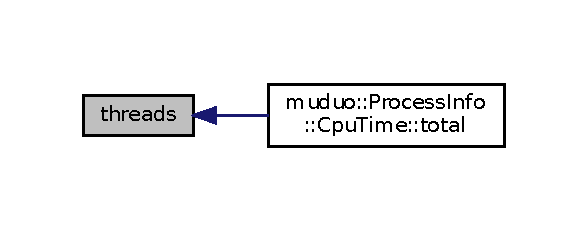
\includegraphics[width=282pt]{namespacemuduo_1_1ProcessInfo_a360aafb2759971d7c8190b1a60f7dc03_icgraph}
\end{center}
\end{figure}
\mbox{\Hypertarget{namespacemuduo_1_1ProcessInfo_a7d3faa2d63f4cf7b8ba073a3daf7ffb1}\label{namespacemuduo_1_1ProcessInfo_a7d3faa2d63f4cf7b8ba073a3daf7ffb1}} 
\index{muduo\+::\+Process\+Info@{muduo\+::\+Process\+Info}!thread\+Stat@{thread\+Stat}}
\index{thread\+Stat@{thread\+Stat}!muduo\+::\+Process\+Info@{muduo\+::\+Process\+Info}}
\subsubsection{\texorpdfstring{thread\+Stat()}{threadStat()}}
{\footnotesize\ttfamily string muduo\+::\+Process\+Info\+::thread\+Stat (\begin{DoxyParamCaption}{ }\end{DoxyParamCaption})}



read /proc/self/task/tid/stat 

\mbox{\Hypertarget{namespacemuduo_1_1ProcessInfo_a056245f62bbe6e8abdcd42171a432aac}\label{namespacemuduo_1_1ProcessInfo_a056245f62bbe6e8abdcd42171a432aac}} 
\index{muduo\+::\+Process\+Info@{muduo\+::\+Process\+Info}!uid@{uid}}
\index{uid@{uid}!muduo\+::\+Process\+Info@{muduo\+::\+Process\+Info}}
\subsubsection{\texorpdfstring{uid()}{uid()}}
{\footnotesize\ttfamily uid\+\_\+t muduo\+::\+Process\+Info\+::uid (\begin{DoxyParamCaption}{ }\end{DoxyParamCaption})}

\mbox{\Hypertarget{namespacemuduo_1_1ProcessInfo_a54e6907a19c94da2cf5db8dcad530262}\label{namespacemuduo_1_1ProcessInfo_a54e6907a19c94da2cf5db8dcad530262}} 
\index{muduo\+::\+Process\+Info@{muduo\+::\+Process\+Info}!username@{username}}
\index{username@{username}!muduo\+::\+Process\+Info@{muduo\+::\+Process\+Info}}
\subsubsection{\texorpdfstring{username()}{username()}}
{\footnotesize\ttfamily string muduo\+::\+Process\+Info\+::username (\begin{DoxyParamCaption}{ }\end{DoxyParamCaption})}


\hypertarget{namespacemuduo_1_1sockets}{}\section{muduo\+:\+:sockets 命名空间参考}
\label{namespacemuduo_1_1sockets}\index{muduo\+::sockets@{muduo\+::sockets}}
\subsection*{函数}
\begin{DoxyCompactItemize}
\item 
uint64\+\_\+t \hyperlink{namespacemuduo_1_1sockets_a6cf7699b950ed4dfbc170a6ff9f71450}{host\+To\+Network64} (uint64\+\_\+t host64)
\item 
uint32\+\_\+t \hyperlink{namespacemuduo_1_1sockets_a937a8685473c938d339f02a8c6d395b6}{host\+To\+Network32} (uint32\+\_\+t host32)
\item 
uint16\+\_\+t \hyperlink{namespacemuduo_1_1sockets_a2c7a9f8e753e01c481aaf287251fa18e}{host\+To\+Network16} (uint16\+\_\+t host16)
\item 
uint64\+\_\+t \hyperlink{namespacemuduo_1_1sockets_ae5a926be124d52254860b4e93a5d1f31}{network\+To\+Host64} (uint64\+\_\+t net64)
\item 
uint32\+\_\+t \hyperlink{namespacemuduo_1_1sockets_a5846c926ef43813d8b8440b6b3a43633}{network\+To\+Host32} (uint32\+\_\+t net32)
\item 
uint16\+\_\+t \hyperlink{namespacemuduo_1_1sockets_aeeb31294e44fee5ecfc4b32f420f6d5d}{network\+To\+Host16} (uint16\+\_\+t net16)
\item 
int \hyperlink{namespacemuduo_1_1sockets_a91269e56d86b2e78e693b330e5c665aa}{create\+Nonblocking\+Or\+Die} ()
\item 
int \hyperlink{namespacemuduo_1_1sockets_a349a8d2188d9632596b2e5213cb16436}{connect} (int sockfd, const struct sockaddr\+\_\+in \&addr)
\item 
void \hyperlink{namespacemuduo_1_1sockets_a8fe4065cd24e49e158dd1c16cd693ae1}{bind\+Or\+Die} (int sockfd, const struct sockaddr\+\_\+in \&addr)
\item 
void \hyperlink{namespacemuduo_1_1sockets_a379cec5f383764a3696d9615bd344529}{listen\+Or\+Die} (int sockfd)
\item 
int \hyperlink{namespacemuduo_1_1sockets_a5fe7cd11cb2662939917285c51b3f992}{accept} (int sockfd, struct sockaddr\+\_\+in $\ast$addr)
\item 
void \hyperlink{namespacemuduo_1_1sockets_acb275b6d8b5979229bae664cb7ee14da}{close} (int sockfd)
\item 
void \hyperlink{namespacemuduo_1_1sockets_a549ec5e856fec6f111aeb481cca9e622}{shutdown\+Write} (int sockfd)
\item 
void \hyperlink{namespacemuduo_1_1sockets_adbdc909d04fd53860d9175b51755b0ae}{to\+Host\+Port} (char $\ast$buf, size\+\_\+t size, const struct sockaddr\+\_\+in \&addr)
\item 
void \hyperlink{namespacemuduo_1_1sockets_ae40b8bfde260835c9034bfaea0fb4ee0}{from\+Host\+Port} (const char $\ast$ip, uint16\+\_\+t port, struct sockaddr\+\_\+in $\ast$addr)
\item 
struct sockaddr\+\_\+in \hyperlink{namespacemuduo_1_1sockets_a4b4793e2d3f77da7bab38cfb52274075}{get\+Local\+Addr} (int sockfd)
\item 
struct sockaddr\+\_\+in \hyperlink{namespacemuduo_1_1sockets_ad095a2bf0c44507c945d04f8346f2817}{get\+Peer\+Addr} (int sockfd)
\item 
int \hyperlink{namespacemuduo_1_1sockets_a80bd626331e049209f59d11c80a8b539}{get\+Socket\+Error} (int sockfd)
\item 
bool \hyperlink{namespacemuduo_1_1sockets_ae3b7d08b5cb176e9d67580a0a1fd57fb}{is\+Self\+Connect} (int sockfd)
\end{DoxyCompactItemize}


\subsection{函数说明}
\mbox{\Hypertarget{namespacemuduo_1_1sockets_a5fe7cd11cb2662939917285c51b3f992}\label{namespacemuduo_1_1sockets_a5fe7cd11cb2662939917285c51b3f992}} 
\index{muduo\+::sockets@{muduo\+::sockets}!accept@{accept}}
\index{accept@{accept}!muduo\+::sockets@{muduo\+::sockets}}
\subsubsection{\texorpdfstring{accept()}{accept()}}
{\footnotesize\ttfamily int accept (\begin{DoxyParamCaption}\item[{int}]{sockfd,  }\item[{struct sockaddr\+\_\+in $\ast$}]{addr }\end{DoxyParamCaption})}



在文件 Sockets\+Ops.\+cc 第 78 行定义.



参考 L\+O\+G\+\_\+\+F\+A\+T\+AL, L\+O\+G\+\_\+\+S\+Y\+S\+E\+RR , 以及 muduo\+::net\+::sockets\+::sockaddr\+\_\+cast().



参考自 Socket\+::accept() , 以及 network\+To\+Host16().

函数调用图\+:
\nopagebreak
\begin{figure}[H]
\begin{center}
\leavevmode
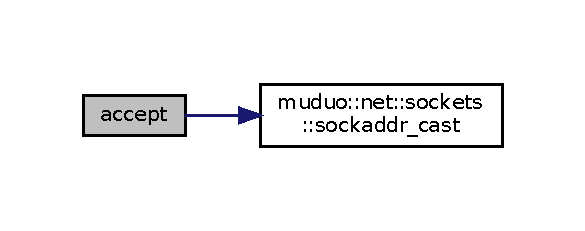
\includegraphics[width=281pt]{namespacemuduo_1_1sockets_a5fe7cd11cb2662939917285c51b3f992_cgraph}
\end{center}
\end{figure}
这是这个函数的调用关系图\+:
\nopagebreak
\begin{figure}[H]
\begin{center}
\leavevmode
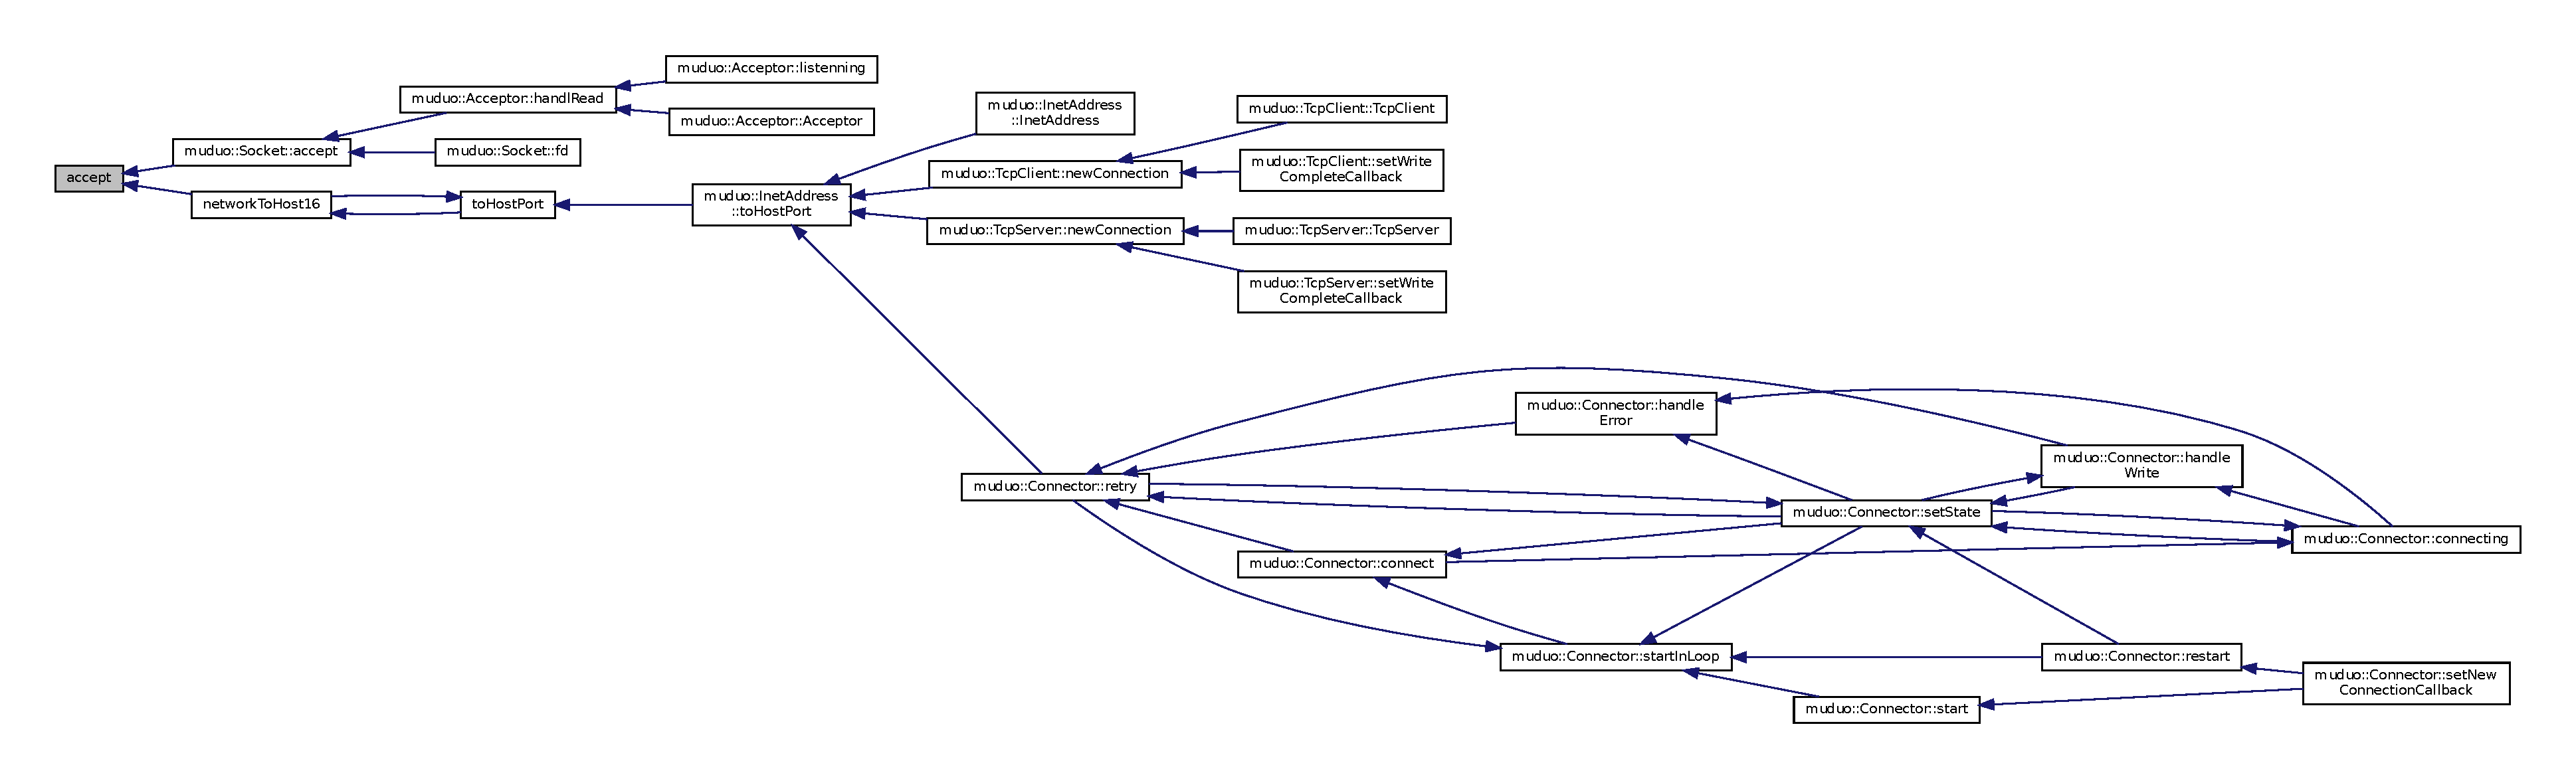
\includegraphics[width=350pt]{namespacemuduo_1_1sockets_a5fe7cd11cb2662939917285c51b3f992_icgraph}
\end{center}
\end{figure}
\mbox{\Hypertarget{namespacemuduo_1_1sockets_a8fe4065cd24e49e158dd1c16cd693ae1}\label{namespacemuduo_1_1sockets_a8fe4065cd24e49e158dd1c16cd693ae1}} 
\index{muduo\+::sockets@{muduo\+::sockets}!bind\+Or\+Die@{bind\+Or\+Die}}
\index{bind\+Or\+Die@{bind\+Or\+Die}!muduo\+::sockets@{muduo\+::sockets}}
\subsubsection{\texorpdfstring{bind\+Or\+Die()}{bindOrDie()}}
{\footnotesize\ttfamily void bind\+Or\+Die (\begin{DoxyParamCaption}\item[{int}]{sockfd,  }\item[{const struct sockaddr\+\_\+in \&}]{addr }\end{DoxyParamCaption})}



在文件 Sockets\+Ops.\+cc 第 64 行定义.



参考 L\+O\+G\+\_\+\+S\+Y\+S\+F\+A\+T\+AL , 以及 muduo\+::net\+::sockets\+::sockaddr\+\_\+cast().



参考自 Socket\+::bind\+Address() , 以及 network\+To\+Host16().

函数调用图\+:
\nopagebreak
\begin{figure}[H]
\begin{center}
\leavevmode
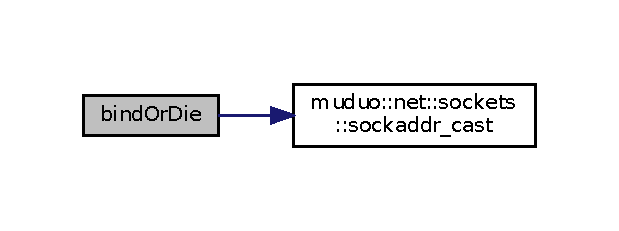
\includegraphics[width=297pt]{namespacemuduo_1_1sockets_a8fe4065cd24e49e158dd1c16cd693ae1_cgraph}
\end{center}
\end{figure}
这是这个函数的调用关系图\+:
\nopagebreak
\begin{figure}[H]
\begin{center}
\leavevmode
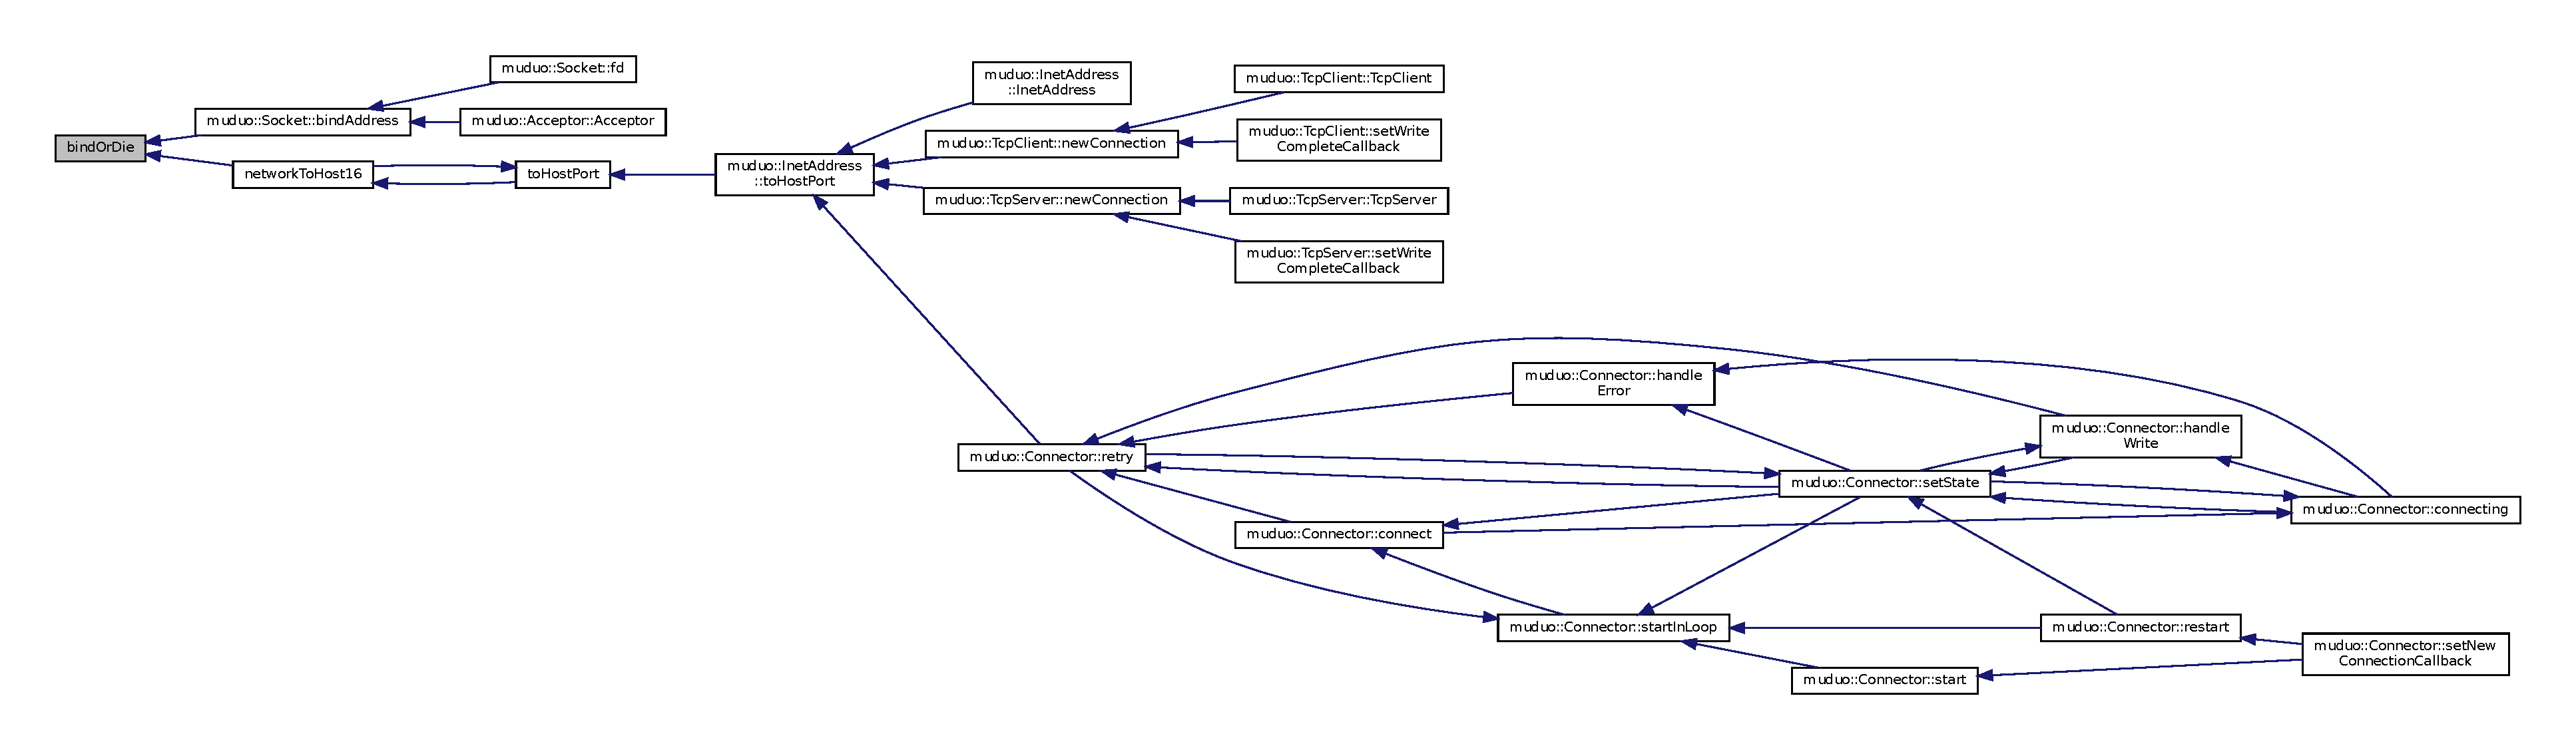
\includegraphics[width=350pt]{namespacemuduo_1_1sockets_a8fe4065cd24e49e158dd1c16cd693ae1_icgraph}
\end{center}
\end{figure}
\mbox{\Hypertarget{namespacemuduo_1_1sockets_acb275b6d8b5979229bae664cb7ee14da}\label{namespacemuduo_1_1sockets_acb275b6d8b5979229bae664cb7ee14da}} 
\index{muduo\+::sockets@{muduo\+::sockets}!close@{close}}
\index{close@{close}!muduo\+::sockets@{muduo\+::sockets}}
\subsubsection{\texorpdfstring{close()}{close()}}
{\footnotesize\ttfamily void close (\begin{DoxyParamCaption}\item[{int}]{sockfd }\end{DoxyParamCaption})}



在文件 Sockets\+Ops.\+cc 第 125 行定义.



参考 L\+O\+G\+\_\+\+S\+Y\+S\+E\+RR.



参考自 Connector\+::connect(), Connector\+::handle\+Write(), Acceptor\+::handl\+Read(), network\+To\+Host16(), Connector\+::retry(), E\+Poller\+::$\sim$\+E\+Poller(), Event\+Loop\+::$\sim$\+Event\+Loop(), Socket\+::$\sim$\+Socket() , 以及 Timer\+Queue\+::$\sim$\+Timer\+Queue().

这是这个函数的调用关系图\+:
\nopagebreak
\begin{figure}[H]
\begin{center}
\leavevmode
\includegraphics[width=350pt]{namespacemuduo_1_1sockets_acb275b6d8b5979229bae664cb7ee14da_icgraph}
\end{center}
\end{figure}
\mbox{\Hypertarget{namespacemuduo_1_1sockets_a349a8d2188d9632596b2e5213cb16436}\label{namespacemuduo_1_1sockets_a349a8d2188d9632596b2e5213cb16436}} 
\index{muduo\+::sockets@{muduo\+::sockets}!connect@{connect}}
\index{connect@{connect}!muduo\+::sockets@{muduo\+::sockets}}
\subsubsection{\texorpdfstring{connect()}{connect()}}
{\footnotesize\ttfamily int connect (\begin{DoxyParamCaption}\item[{int}]{sockfd,  }\item[{const struct sockaddr\+\_\+in \&}]{addr }\end{DoxyParamCaption})}



在文件 Sockets\+Ops.\+cc 第 60 行定义.



参考 muduo\+::net\+::sockets\+::sockaddr\+\_\+cast().



参考自 Connector\+::connect() , 以及 network\+To\+Host16().

函数调用图\+:
\nopagebreak
\begin{figure}[H]
\begin{center}
\leavevmode
\includegraphics[width=287pt]{namespacemuduo_1_1sockets_a349a8d2188d9632596b2e5213cb16436_cgraph}
\end{center}
\end{figure}
这是这个函数的调用关系图\+:
\nopagebreak
\begin{figure}[H]
\begin{center}
\leavevmode
\includegraphics[width=350pt]{namespacemuduo_1_1sockets_a349a8d2188d9632596b2e5213cb16436_icgraph}
\end{center}
\end{figure}
\mbox{\Hypertarget{namespacemuduo_1_1sockets_a91269e56d86b2e78e693b330e5c665aa}\label{namespacemuduo_1_1sockets_a91269e56d86b2e78e693b330e5c665aa}} 
\index{muduo\+::sockets@{muduo\+::sockets}!create\+Nonblocking\+Or\+Die@{create\+Nonblocking\+Or\+Die}}
\index{create\+Nonblocking\+Or\+Die@{create\+Nonblocking\+Or\+Die}!muduo\+::sockets@{muduo\+::sockets}}
\subsubsection{\texorpdfstring{create\+Nonblocking\+Or\+Die()}{createNonblockingOrDie()}}
{\footnotesize\ttfamily int create\+Nonblocking\+Or\+Die (\begin{DoxyParamCaption}{ }\end{DoxyParamCaption})}

Creates a non-\/blocking socket file descriptor, abort if any error. 

在文件 Sockets\+Ops.\+cc 第 42 行定义.



参考 L\+O\+G\+\_\+\+S\+Y\+S\+F\+A\+T\+AL.



参考自 Connector\+::connect() , 以及 network\+To\+Host16().

这是这个函数的调用关系图\+:
\nopagebreak
\begin{figure}[H]
\begin{center}
\leavevmode
\includegraphics[width=350pt]{namespacemuduo_1_1sockets_a91269e56d86b2e78e693b330e5c665aa_icgraph}
\end{center}
\end{figure}
\mbox{\Hypertarget{namespacemuduo_1_1sockets_ae40b8bfde260835c9034bfaea0fb4ee0}\label{namespacemuduo_1_1sockets_ae40b8bfde260835c9034bfaea0fb4ee0}} 
\index{muduo\+::sockets@{muduo\+::sockets}!from\+Host\+Port@{from\+Host\+Port}}
\index{from\+Host\+Port@{from\+Host\+Port}!muduo\+::sockets@{muduo\+::sockets}}
\subsubsection{\texorpdfstring{from\+Host\+Port()}{fromHostPort()}}
{\footnotesize\ttfamily void from\+Host\+Port (\begin{DoxyParamCaption}\item[{const char $\ast$}]{ip,  }\item[{uint16\+\_\+t}]{port,  }\item[{struct sockaddr\+\_\+in $\ast$}]{addr }\end{DoxyParamCaption})}



在文件 Sockets\+Ops.\+cc 第 150 行定义.



参考 muduo\+::net\+::sockets\+::host\+To\+Network16() , 以及 L\+O\+G\+\_\+\+S\+Y\+S\+E\+RR.



参考自 Inet\+Address\+::\+Inet\+Address() , 以及 network\+To\+Host16().

函数调用图\+:
\nopagebreak
\begin{figure}[H]
\begin{center}
\leavevmode
\includegraphics[width=314pt]{namespacemuduo_1_1sockets_ae40b8bfde260835c9034bfaea0fb4ee0_cgraph}
\end{center}
\end{figure}
这是这个函数的调用关系图\+:
\nopagebreak
\begin{figure}[H]
\begin{center}
\leavevmode
\includegraphics[width=350pt]{namespacemuduo_1_1sockets_ae40b8bfde260835c9034bfaea0fb4ee0_icgraph}
\end{center}
\end{figure}
\mbox{\Hypertarget{namespacemuduo_1_1sockets_a4b4793e2d3f77da7bab38cfb52274075}\label{namespacemuduo_1_1sockets_a4b4793e2d3f77da7bab38cfb52274075}} 
\index{muduo\+::sockets@{muduo\+::sockets}!get\+Local\+Addr@{get\+Local\+Addr}}
\index{get\+Local\+Addr@{get\+Local\+Addr}!muduo\+::sockets@{muduo\+::sockets}}
\subsubsection{\texorpdfstring{get\+Local\+Addr()}{getLocalAddr()}}
{\footnotesize\ttfamily struct sockaddr\+\_\+in get\+Local\+Addr (\begin{DoxyParamCaption}\item[{int}]{sockfd }\end{DoxyParamCaption})}



在文件 Sockets\+Ops.\+cc 第 162 行定义.



参考 L\+O\+G\+\_\+\+S\+Y\+S\+E\+RR , 以及 muduo\+::net\+::sockets\+::sockaddr\+\_\+cast().



参考自 is\+Self\+Connect(), Tcp\+Client\+::new\+Connection() , 以及 Tcp\+Server\+::new\+Connection().

函数调用图\+:
\nopagebreak
\begin{figure}[H]
\begin{center}
\leavevmode
\includegraphics[width=312pt]{namespacemuduo_1_1sockets_a4b4793e2d3f77da7bab38cfb52274075_cgraph}
\end{center}
\end{figure}
这是这个函数的调用关系图\+:
\nopagebreak
\begin{figure}[H]
\begin{center}
\leavevmode
\includegraphics[width=350pt]{namespacemuduo_1_1sockets_a4b4793e2d3f77da7bab38cfb52274075_icgraph}
\end{center}
\end{figure}
\mbox{\Hypertarget{namespacemuduo_1_1sockets_ad095a2bf0c44507c945d04f8346f2817}\label{namespacemuduo_1_1sockets_ad095a2bf0c44507c945d04f8346f2817}} 
\index{muduo\+::sockets@{muduo\+::sockets}!get\+Peer\+Addr@{get\+Peer\+Addr}}
\index{get\+Peer\+Addr@{get\+Peer\+Addr}!muduo\+::sockets@{muduo\+::sockets}}
\subsubsection{\texorpdfstring{get\+Peer\+Addr()}{getPeerAddr()}}
{\footnotesize\ttfamily struct sockaddr\+\_\+in get\+Peer\+Addr (\begin{DoxyParamCaption}\item[{int}]{sockfd }\end{DoxyParamCaption})}



在文件 Sockets\+Ops.\+cc 第 172 行定义.



参考 L\+O\+G\+\_\+\+S\+Y\+S\+E\+RR , 以及 muduo\+::net\+::sockets\+::sockaddr\+\_\+cast().



参考自 is\+Self\+Connect() , 以及 Tcp\+Client\+::new\+Connection().

函数调用图\+:
\nopagebreak
\begin{figure}[H]
\begin{center}
\leavevmode
\includegraphics[width=309pt]{namespacemuduo_1_1sockets_ad095a2bf0c44507c945d04f8346f2817_cgraph}
\end{center}
\end{figure}
这是这个函数的调用关系图\+:
\nopagebreak
\begin{figure}[H]
\begin{center}
\leavevmode
\includegraphics[width=350pt]{namespacemuduo_1_1sockets_ad095a2bf0c44507c945d04f8346f2817_icgraph}
\end{center}
\end{figure}
\mbox{\Hypertarget{namespacemuduo_1_1sockets_a80bd626331e049209f59d11c80a8b539}\label{namespacemuduo_1_1sockets_a80bd626331e049209f59d11c80a8b539}} 
\index{muduo\+::sockets@{muduo\+::sockets}!get\+Socket\+Error@{get\+Socket\+Error}}
\index{get\+Socket\+Error@{get\+Socket\+Error}!muduo\+::sockets@{muduo\+::sockets}}
\subsubsection{\texorpdfstring{get\+Socket\+Error()}{getSocketError()}}
{\footnotesize\ttfamily int get\+Socket\+Error (\begin{DoxyParamCaption}\item[{int}]{sockfd }\end{DoxyParamCaption})}



在文件 Sockets\+Ops.\+cc 第 182 行定义.



参考自 Connector\+::handle\+Error(), Tcp\+Connection\+::handle\+Error(), Connector\+::handle\+Write() , 以及 network\+To\+Host16().

这是这个函数的调用关系图\+:
\nopagebreak
\begin{figure}[H]
\begin{center}
\leavevmode
\includegraphics[width=350pt]{namespacemuduo_1_1sockets_a80bd626331e049209f59d11c80a8b539_icgraph}
\end{center}
\end{figure}
\mbox{\Hypertarget{namespacemuduo_1_1sockets_a2c7a9f8e753e01c481aaf287251fa18e}\label{namespacemuduo_1_1sockets_a2c7a9f8e753e01c481aaf287251fa18e}} 
\index{muduo\+::sockets@{muduo\+::sockets}!host\+To\+Network16@{host\+To\+Network16}}
\index{host\+To\+Network16@{host\+To\+Network16}!muduo\+::sockets@{muduo\+::sockets}}
\subsubsection{\texorpdfstring{host\+To\+Network16()}{hostToNetwork16()}}
{\footnotesize\ttfamily uint16\+\_\+t muduo\+::sockets\+::host\+To\+Network16 (\begin{DoxyParamCaption}\item[{uint16\+\_\+t}]{host16 }\end{DoxyParamCaption})\hspace{0.3cm}{\ttfamily [inline]}}



在文件 Sockets\+Ops.\+h 第 20 行定义.



参考自 Inet\+Address\+::\+Inet\+Address().

这是这个函数的调用关系图\+:
\nopagebreak
\begin{figure}[H]
\begin{center}
\leavevmode
\includegraphics[width=331pt]{namespacemuduo_1_1sockets_a2c7a9f8e753e01c481aaf287251fa18e_icgraph}
\end{center}
\end{figure}
\mbox{\Hypertarget{namespacemuduo_1_1sockets_a937a8685473c938d339f02a8c6d395b6}\label{namespacemuduo_1_1sockets_a937a8685473c938d339f02a8c6d395b6}} 
\index{muduo\+::sockets@{muduo\+::sockets}!host\+To\+Network32@{host\+To\+Network32}}
\index{host\+To\+Network32@{host\+To\+Network32}!muduo\+::sockets@{muduo\+::sockets}}
\subsubsection{\texorpdfstring{host\+To\+Network32()}{hostToNetwork32()}}
{\footnotesize\ttfamily uint32\+\_\+t muduo\+::sockets\+::host\+To\+Network32 (\begin{DoxyParamCaption}\item[{uint32\+\_\+t}]{host32 }\end{DoxyParamCaption})\hspace{0.3cm}{\ttfamily [inline]}}



在文件 Sockets\+Ops.\+h 第 16 行定义.



参考自 Inet\+Address\+::\+Inet\+Address().

这是这个函数的调用关系图\+:
\nopagebreak
\begin{figure}[H]
\begin{center}
\leavevmode
\includegraphics[width=331pt]{namespacemuduo_1_1sockets_a937a8685473c938d339f02a8c6d395b6_icgraph}
\end{center}
\end{figure}
\mbox{\Hypertarget{namespacemuduo_1_1sockets_a6cf7699b950ed4dfbc170a6ff9f71450}\label{namespacemuduo_1_1sockets_a6cf7699b950ed4dfbc170a6ff9f71450}} 
\index{muduo\+::sockets@{muduo\+::sockets}!host\+To\+Network64@{host\+To\+Network64}}
\index{host\+To\+Network64@{host\+To\+Network64}!muduo\+::sockets@{muduo\+::sockets}}
\subsubsection{\texorpdfstring{host\+To\+Network64()}{hostToNetwork64()}}
{\footnotesize\ttfamily uint64\+\_\+t muduo\+::sockets\+::host\+To\+Network64 (\begin{DoxyParamCaption}\item[{uint64\+\_\+t}]{host64 }\end{DoxyParamCaption})\hspace{0.3cm}{\ttfamily [inline]}}



在文件 Sockets\+Ops.\+h 第 12 行定义.

\mbox{\Hypertarget{namespacemuduo_1_1sockets_ae3b7d08b5cb176e9d67580a0a1fd57fb}\label{namespacemuduo_1_1sockets_ae3b7d08b5cb176e9d67580a0a1fd57fb}} 
\index{muduo\+::sockets@{muduo\+::sockets}!is\+Self\+Connect@{is\+Self\+Connect}}
\index{is\+Self\+Connect@{is\+Self\+Connect}!muduo\+::sockets@{muduo\+::sockets}}
\subsubsection{\texorpdfstring{is\+Self\+Connect()}{isSelfConnect()}}
{\footnotesize\ttfamily bool is\+Self\+Connect (\begin{DoxyParamCaption}\item[{int}]{sockfd }\end{DoxyParamCaption})}



在文件 Sockets\+Ops.\+cc 第 198 行定义.



参考 get\+Local\+Addr() , 以及 get\+Peer\+Addr().



参考自 Connector\+::handle\+Write() , 以及 network\+To\+Host16().

函数调用图\+:
\nopagebreak
\begin{figure}[H]
\begin{center}
\leavevmode
\includegraphics[width=350pt]{namespacemuduo_1_1sockets_ae3b7d08b5cb176e9d67580a0a1fd57fb_cgraph}
\end{center}
\end{figure}
这是这个函数的调用关系图\+:
\nopagebreak
\begin{figure}[H]
\begin{center}
\leavevmode
\includegraphics[width=350pt]{namespacemuduo_1_1sockets_ae3b7d08b5cb176e9d67580a0a1fd57fb_icgraph}
\end{center}
\end{figure}
\mbox{\Hypertarget{namespacemuduo_1_1sockets_a379cec5f383764a3696d9615bd344529}\label{namespacemuduo_1_1sockets_a379cec5f383764a3696d9615bd344529}} 
\index{muduo\+::sockets@{muduo\+::sockets}!listen\+Or\+Die@{listen\+Or\+Die}}
\index{listen\+Or\+Die@{listen\+Or\+Die}!muduo\+::sockets@{muduo\+::sockets}}
\subsubsection{\texorpdfstring{listen\+Or\+Die()}{listenOrDie()}}
{\footnotesize\ttfamily void listen\+Or\+Die (\begin{DoxyParamCaption}\item[{int}]{sockfd }\end{DoxyParamCaption})}



在文件 Sockets\+Ops.\+cc 第 71 行定义.



参考 L\+O\+G\+\_\+\+S\+Y\+S\+F\+A\+T\+AL.



参考自 Socket\+::listen() , 以及 network\+To\+Host16().

这是这个函数的调用关系图\+:
\nopagebreak
\begin{figure}[H]
\begin{center}
\leavevmode
\includegraphics[width=350pt]{namespacemuduo_1_1sockets_a379cec5f383764a3696d9615bd344529_icgraph}
\end{center}
\end{figure}
\mbox{\Hypertarget{namespacemuduo_1_1sockets_aeeb31294e44fee5ecfc4b32f420f6d5d}\label{namespacemuduo_1_1sockets_aeeb31294e44fee5ecfc4b32f420f6d5d}} 
\index{muduo\+::sockets@{muduo\+::sockets}!network\+To\+Host16@{network\+To\+Host16}}
\index{network\+To\+Host16@{network\+To\+Host16}!muduo\+::sockets@{muduo\+::sockets}}
\subsubsection{\texorpdfstring{network\+To\+Host16()}{networkToHost16()}}
{\footnotesize\ttfamily uint16\+\_\+t muduo\+::sockets\+::network\+To\+Host16 (\begin{DoxyParamCaption}\item[{uint16\+\_\+t}]{net16 }\end{DoxyParamCaption})\hspace{0.3cm}{\ttfamily [inline]}}



在文件 Sockets\+Ops.\+h 第 32 行定义.



参考 accept(), bind\+Or\+Die(), close(), connect(), create\+Nonblocking\+Or\+Die(), from\+Host\+Port(), get\+Socket\+Error(), is\+Self\+Connect(), listen\+Or\+Die(), shutdown\+Write() , 以及 to\+Host\+Port().



参考自 to\+Host\+Port().

函数调用图\+:
\nopagebreak
\begin{figure}[H]
\begin{center}
\leavevmode
\includegraphics[width=350pt]{namespacemuduo_1_1sockets_aeeb31294e44fee5ecfc4b32f420f6d5d_cgraph}
\end{center}
\end{figure}
这是这个函数的调用关系图\+:
\nopagebreak
\begin{figure}[H]
\begin{center}
\leavevmode
\includegraphics[width=350pt]{namespacemuduo_1_1sockets_aeeb31294e44fee5ecfc4b32f420f6d5d_icgraph}
\end{center}
\end{figure}
\mbox{\Hypertarget{namespacemuduo_1_1sockets_a5846c926ef43813d8b8440b6b3a43633}\label{namespacemuduo_1_1sockets_a5846c926ef43813d8b8440b6b3a43633}} 
\index{muduo\+::sockets@{muduo\+::sockets}!network\+To\+Host32@{network\+To\+Host32}}
\index{network\+To\+Host32@{network\+To\+Host32}!muduo\+::sockets@{muduo\+::sockets}}
\subsubsection{\texorpdfstring{network\+To\+Host32()}{networkToHost32()}}
{\footnotesize\ttfamily uint32\+\_\+t muduo\+::sockets\+::network\+To\+Host32 (\begin{DoxyParamCaption}\item[{uint32\+\_\+t}]{net32 }\end{DoxyParamCaption})\hspace{0.3cm}{\ttfamily [inline]}}



在文件 Sockets\+Ops.\+h 第 28 行定义.

\mbox{\Hypertarget{namespacemuduo_1_1sockets_ae5a926be124d52254860b4e93a5d1f31}\label{namespacemuduo_1_1sockets_ae5a926be124d52254860b4e93a5d1f31}} 
\index{muduo\+::sockets@{muduo\+::sockets}!network\+To\+Host64@{network\+To\+Host64}}
\index{network\+To\+Host64@{network\+To\+Host64}!muduo\+::sockets@{muduo\+::sockets}}
\subsubsection{\texorpdfstring{network\+To\+Host64()}{networkToHost64()}}
{\footnotesize\ttfamily uint64\+\_\+t muduo\+::sockets\+::network\+To\+Host64 (\begin{DoxyParamCaption}\item[{uint64\+\_\+t}]{net64 }\end{DoxyParamCaption})\hspace{0.3cm}{\ttfamily [inline]}}



在文件 Sockets\+Ops.\+h 第 24 行定义.

\mbox{\Hypertarget{namespacemuduo_1_1sockets_a549ec5e856fec6f111aeb481cca9e622}\label{namespacemuduo_1_1sockets_a549ec5e856fec6f111aeb481cca9e622}} 
\index{muduo\+::sockets@{muduo\+::sockets}!shutdown\+Write@{shutdown\+Write}}
\index{shutdown\+Write@{shutdown\+Write}!muduo\+::sockets@{muduo\+::sockets}}
\subsubsection{\texorpdfstring{shutdown\+Write()}{shutdownWrite()}}
{\footnotesize\ttfamily void shutdown\+Write (\begin{DoxyParamCaption}\item[{int}]{sockfd }\end{DoxyParamCaption})}



在文件 Sockets\+Ops.\+cc 第 131 行定义.



参考 L\+O\+G\+\_\+\+S\+Y\+S\+E\+RR.



参考自 network\+To\+Host16() , 以及 Socket\+::shutdown\+Write().

这是这个函数的调用关系图\+:
\nopagebreak
\begin{figure}[H]
\begin{center}
\leavevmode
\includegraphics[width=350pt]{namespacemuduo_1_1sockets_a549ec5e856fec6f111aeb481cca9e622_icgraph}
\end{center}
\end{figure}
\mbox{\Hypertarget{namespacemuduo_1_1sockets_adbdc909d04fd53860d9175b51755b0ae}\label{namespacemuduo_1_1sockets_adbdc909d04fd53860d9175b51755b0ae}} 
\index{muduo\+::sockets@{muduo\+::sockets}!to\+Host\+Port@{to\+Host\+Port}}
\index{to\+Host\+Port@{to\+Host\+Port}!muduo\+::sockets@{muduo\+::sockets}}
\subsubsection{\texorpdfstring{to\+Host\+Port()}{toHostPort()}}
{\footnotesize\ttfamily void to\+Host\+Port (\begin{DoxyParamCaption}\item[{char $\ast$}]{buf,  }\item[{size\+\_\+t}]{size,  }\item[{const struct sockaddr\+\_\+in \&}]{addr }\end{DoxyParamCaption})}



在文件 Sockets\+Ops.\+cc 第 137 行定义.



参考 network\+To\+Host16().



参考自 network\+To\+Host16() , 以及 Inet\+Address\+::to\+Host\+Port().

函数调用图\+:
\nopagebreak
\begin{figure}[H]
\begin{center}
\leavevmode
\includegraphics[width=350pt]{namespacemuduo_1_1sockets_adbdc909d04fd53860d9175b51755b0ae_cgraph}
\end{center}
\end{figure}
这是这个函数的调用关系图\+:
\nopagebreak
\begin{figure}[H]
\begin{center}
\leavevmode
\includegraphics[width=350pt]{namespacemuduo_1_1sockets_adbdc909d04fd53860d9175b51755b0ae_icgraph}
\end{center}
\end{figure}

\chapter{类说明}
\hypertarget{classmuduo_1_1Acceptor}{}\section{Acceptor类 参考}
\label{classmuduo_1_1Acceptor}\index{Acceptor@{Acceptor}}


{\ttfamily \#include $<$Acceptor.\+h$>$}



类 Acceptor 继承关系图\+:
\nopagebreak
\begin{figure}[H]
\begin{center}
\leavevmode
\includegraphics[width=249pt]{classmuduo_1_1Acceptor__inherit__graph}
\end{center}
\end{figure}


Acceptor 的协作图\+:
\nopagebreak
\begin{figure}[H]
\begin{center}
\leavevmode
\includegraphics[height=550pt]{classmuduo_1_1Acceptor__coll__graph}
\end{center}
\end{figure}
\subsection*{Public 类型}
\begin{DoxyCompactItemize}
\item 
typedef boost\+::function$<$ void(int sockfd, const \hyperlink{classmuduo_1_1InetAddress}{Inet\+Address} \&)$>$ \hyperlink{classmuduo_1_1Acceptor_ad9da8988c47fddac6b0b91e01e154814}{New\+Connection\+Callback}
\end{DoxyCompactItemize}
\subsection*{Public 成员函数}
\begin{DoxyCompactItemize}
\item 
\hyperlink{classmuduo_1_1Acceptor_a034c2e4c8c39c67bcaa4a47a6fa906fd}{Acceptor} (\hyperlink{classmuduo_1_1EventLoop}{Event\+Loop} $\ast$loop, const \hyperlink{classmuduo_1_1InetAddress}{Inet\+Address} \&listen\+Addr)
\item 
void \hyperlink{classmuduo_1_1Acceptor_a30908d8d30b5333e6288a7430d598cb1}{set\+New\+Connection\+Callback} (const \hyperlink{classmuduo_1_1Acceptor_ad9da8988c47fddac6b0b91e01e154814}{New\+Connection\+Callback} \&cb)
\item 
bool \hyperlink{classmuduo_1_1Acceptor_a43301d614b7aaae820d7ddd7033984f5}{listenning} () const
\item 
void \hyperlink{classmuduo_1_1Acceptor_a458bbe4cf81360301586b2e62a7f9dd2}{listen} ()
\end{DoxyCompactItemize}
\subsection*{Private 成员函数}
\begin{DoxyCompactItemize}
\item 
void \hyperlink{classmuduo_1_1Acceptor_a3459892d34c1eb51b40a53b8062237ca}{handl\+Read} ()
\end{DoxyCompactItemize}
\subsection*{Private 属性}
\begin{DoxyCompactItemize}
\item 
\hyperlink{classmuduo_1_1EventLoop}{Event\+Loop} $\ast$ \hyperlink{classmuduo_1_1Acceptor_a19968f50018d32ac31f5cba0195591ac}{loop\+\_\+}
\item 
\hyperlink{classmuduo_1_1Socket}{Socket} \hyperlink{classmuduo_1_1Acceptor_a5b8432787de199c64a25108a26d4690d}{accept\+Socket\+\_\+}
\item 
\hyperlink{classmuduo_1_1Channel}{Channel} \hyperlink{classmuduo_1_1Acceptor_a32c277ec09ca9c780ddc51b21278c317}{accept\+Channel\+\_\+}
\item 
\hyperlink{classmuduo_1_1Acceptor_ad9da8988c47fddac6b0b91e01e154814}{New\+Connection\+Callback} \hyperlink{classmuduo_1_1Acceptor_a315d8356d0420fe5a89dc67f49c82617}{new\+Connection\+Callback\+\_\+}
\item 
bool \hyperlink{classmuduo_1_1Acceptor_af4e1fb2da4efe5a7bcfff6c2434f966d}{listenning\+\_\+}
\end{DoxyCompactItemize}


\subsection{详细描述}
\hyperlink{classmuduo_1_1Acceptor}{Acceptor} of incoming T\+CP connections. 

在文件 Acceptor.\+h 第 18 行定义.



\subsection{成员类型定义说明}
\mbox{\Hypertarget{classmuduo_1_1Acceptor_ad9da8988c47fddac6b0b91e01e154814}\label{classmuduo_1_1Acceptor_ad9da8988c47fddac6b0b91e01e154814}} 
\index{muduo\+::\+Acceptor@{muduo\+::\+Acceptor}!New\+Connection\+Callback@{New\+Connection\+Callback}}
\index{New\+Connection\+Callback@{New\+Connection\+Callback}!muduo\+::\+Acceptor@{muduo\+::\+Acceptor}}
\subsubsection{\texorpdfstring{New\+Connection\+Callback}{NewConnectionCallback}}
{\footnotesize\ttfamily typedef boost\+::function$<$void(int sockfd, const \hyperlink{classmuduo_1_1InetAddress}{Inet\+Address}\&)$>$ \hyperlink{classmuduo_1_1Acceptor_ad9da8988c47fddac6b0b91e01e154814}{New\+Connection\+Callback}}



在文件 Acceptor.\+h 第 20 行定义.



\subsection{构造及析构函数说明}
\mbox{\Hypertarget{classmuduo_1_1Acceptor_a034c2e4c8c39c67bcaa4a47a6fa906fd}\label{classmuduo_1_1Acceptor_a034c2e4c8c39c67bcaa4a47a6fa906fd}} 
\index{muduo\+::\+Acceptor@{muduo\+::\+Acceptor}!Acceptor@{Acceptor}}
\index{Acceptor@{Acceptor}!muduo\+::\+Acceptor@{muduo\+::\+Acceptor}}
\subsubsection{\texorpdfstring{Acceptor()}{Acceptor()}}
{\footnotesize\ttfamily \hyperlink{classmuduo_1_1Acceptor}{Acceptor} (\begin{DoxyParamCaption}\item[{\hyperlink{classmuduo_1_1EventLoop}{Event\+Loop} $\ast$}]{loop,  }\item[{const \hyperlink{classmuduo_1_1InetAddress}{Inet\+Address} \&}]{listen\+Addr }\end{DoxyParamCaption})}



在文件 Acceptor.\+cc 第 12 行定义.



参考 Acceptor\+::accept\+Channel\+\_\+, Acceptor\+::accept\+Socket\+\_\+, Socket\+::bind\+Address(), Acceptor\+::handl\+Read(), Channel\+::set\+Read\+Callback() , 以及 Socket\+::set\+Reuse\+Addr().

函数调用图\+:
\nopagebreak
\begin{figure}[H]
\begin{center}
\leavevmode
\includegraphics[width=350pt]{classmuduo_1_1Acceptor_a034c2e4c8c39c67bcaa4a47a6fa906fd_cgraph}
\end{center}
\end{figure}


\subsection{成员函数说明}
\mbox{\Hypertarget{classmuduo_1_1Acceptor_a3459892d34c1eb51b40a53b8062237ca}\label{classmuduo_1_1Acceptor_a3459892d34c1eb51b40a53b8062237ca}} 
\index{muduo\+::\+Acceptor@{muduo\+::\+Acceptor}!handl\+Read@{handl\+Read}}
\index{handl\+Read@{handl\+Read}!muduo\+::\+Acceptor@{muduo\+::\+Acceptor}}
\subsubsection{\texorpdfstring{handl\+Read()}{handlRead()}}
{\footnotesize\ttfamily void handl\+Read (\begin{DoxyParamCaption}{ }\end{DoxyParamCaption})\hspace{0.3cm}{\ttfamily [private]}}



在文件 Acceptor.\+cc 第 29 行定义.



参考 Socket\+::accept(), Acceptor\+::accept\+Socket\+\_\+, Event\+Loop\+::assert\+In\+Loop\+Thread(), muduo\+::sockets\+::close(), Acceptor\+::loop\+\_\+ , 以及 Acceptor\+::new\+Connection\+Callback\+\_\+.



参考自 Acceptor\+::\+Acceptor() , 以及 Acceptor\+::listenning().

函数调用图\+:
\nopagebreak
\begin{figure}[H]
\begin{center}
\leavevmode
\includegraphics[width=350pt]{classmuduo_1_1Acceptor_a3459892d34c1eb51b40a53b8062237ca_cgraph}
\end{center}
\end{figure}
这是这个函数的调用关系图\+:
\nopagebreak
\begin{figure}[H]
\begin{center}
\leavevmode
\includegraphics[width=249pt]{classmuduo_1_1Acceptor_a3459892d34c1eb51b40a53b8062237ca_icgraph}
\end{center}
\end{figure}
\mbox{\Hypertarget{classmuduo_1_1Acceptor_a458bbe4cf81360301586b2e62a7f9dd2}\label{classmuduo_1_1Acceptor_a458bbe4cf81360301586b2e62a7f9dd2}} 
\index{muduo\+::\+Acceptor@{muduo\+::\+Acceptor}!listen@{listen}}
\index{listen@{listen}!muduo\+::\+Acceptor@{muduo\+::\+Acceptor}}
\subsubsection{\texorpdfstring{listen()}{listen()}}
{\footnotesize\ttfamily void listen (\begin{DoxyParamCaption}{ }\end{DoxyParamCaption})}



在文件 Acceptor.\+cc 第 22 行定义.



参考 Acceptor\+::accept\+Channel\+\_\+, Acceptor\+::accept\+Socket\+\_\+, Event\+Loop\+::assert\+In\+Loop\+Thread(), Channel\+::enable\+Reading(), Socket\+::listen(), Acceptor\+::listenning\+\_\+ , 以及 Acceptor\+::loop\+\_\+.



参考自 Acceptor\+::listenning() , 以及 Tcp\+Server\+::start().

函数调用图\+:
\nopagebreak
\begin{figure}[H]
\begin{center}
\leavevmode
\includegraphics[width=350pt]{classmuduo_1_1Acceptor_a458bbe4cf81360301586b2e62a7f9dd2_cgraph}
\end{center}
\end{figure}
这是这个函数的调用关系图\+:
\nopagebreak
\begin{figure}[H]
\begin{center}
\leavevmode
\includegraphics[width=350pt]{classmuduo_1_1Acceptor_a458bbe4cf81360301586b2e62a7f9dd2_icgraph}
\end{center}
\end{figure}
\mbox{\Hypertarget{classmuduo_1_1Acceptor_a43301d614b7aaae820d7ddd7033984f5}\label{classmuduo_1_1Acceptor_a43301d614b7aaae820d7ddd7033984f5}} 
\index{muduo\+::\+Acceptor@{muduo\+::\+Acceptor}!listenning@{listenning}}
\index{listenning@{listenning}!muduo\+::\+Acceptor@{muduo\+::\+Acceptor}}
\subsubsection{\texorpdfstring{listenning()}{listenning()}}
{\footnotesize\ttfamily bool listenning (\begin{DoxyParamCaption}{ }\end{DoxyParamCaption}) const\hspace{0.3cm}{\ttfamily [inline]}}



在文件 Acceptor.\+h 第 28 行定义.



参考 Acceptor\+::handl\+Read(), Acceptor\+::listen() , 以及 Acceptor\+::listenning\+\_\+.

函数调用图\+:
\nopagebreak
\begin{figure}[H]
\begin{center}
\leavevmode
\includegraphics[width=350pt]{classmuduo_1_1Acceptor_a43301d614b7aaae820d7ddd7033984f5_cgraph}
\end{center}
\end{figure}
\mbox{\Hypertarget{classmuduo_1_1Acceptor_a30908d8d30b5333e6288a7430d598cb1}\label{classmuduo_1_1Acceptor_a30908d8d30b5333e6288a7430d598cb1}} 
\index{muduo\+::\+Acceptor@{muduo\+::\+Acceptor}!set\+New\+Connection\+Callback@{set\+New\+Connection\+Callback}}
\index{set\+New\+Connection\+Callback@{set\+New\+Connection\+Callback}!muduo\+::\+Acceptor@{muduo\+::\+Acceptor}}
\subsubsection{\texorpdfstring{set\+New\+Connection\+Callback()}{setNewConnectionCallback()}}
{\footnotesize\ttfamily void set\+New\+Connection\+Callback (\begin{DoxyParamCaption}\item[{const \hyperlink{classmuduo_1_1Acceptor_ad9da8988c47fddac6b0b91e01e154814}{New\+Connection\+Callback} \&}]{cb }\end{DoxyParamCaption})\hspace{0.3cm}{\ttfamily [inline]}}



在文件 Acceptor.\+h 第 24 行定义.



参考 Acceptor\+::new\+Connection\+Callback\+\_\+.



\subsection{类成员变量说明}
\mbox{\Hypertarget{classmuduo_1_1Acceptor_a32c277ec09ca9c780ddc51b21278c317}\label{classmuduo_1_1Acceptor_a32c277ec09ca9c780ddc51b21278c317}} 
\index{muduo\+::\+Acceptor@{muduo\+::\+Acceptor}!accept\+Channel\+\_\+@{accept\+Channel\+\_\+}}
\index{accept\+Channel\+\_\+@{accept\+Channel\+\_\+}!muduo\+::\+Acceptor@{muduo\+::\+Acceptor}}
\subsubsection{\texorpdfstring{accept\+Channel\+\_\+}{acceptChannel\_}}
{\footnotesize\ttfamily \hyperlink{classmuduo_1_1Channel}{Channel} accept\+Channel\+\_\+\hspace{0.3cm}{\ttfamily [private]}}



在文件 Acceptor.\+h 第 39 行定义.



参考自 Acceptor\+::\+Acceptor() , 以及 Acceptor\+::listen().

\mbox{\Hypertarget{classmuduo_1_1Acceptor_a5b8432787de199c64a25108a26d4690d}\label{classmuduo_1_1Acceptor_a5b8432787de199c64a25108a26d4690d}} 
\index{muduo\+::\+Acceptor@{muduo\+::\+Acceptor}!accept\+Socket\+\_\+@{accept\+Socket\+\_\+}}
\index{accept\+Socket\+\_\+@{accept\+Socket\+\_\+}!muduo\+::\+Acceptor@{muduo\+::\+Acceptor}}
\subsubsection{\texorpdfstring{accept\+Socket\+\_\+}{acceptSocket\_}}
{\footnotesize\ttfamily \hyperlink{classmuduo_1_1Socket}{Socket} accept\+Socket\+\_\+\hspace{0.3cm}{\ttfamily [private]}}



在文件 Acceptor.\+h 第 38 行定义.



参考自 Acceptor\+::\+Acceptor(), Acceptor\+::handl\+Read() , 以及 Acceptor\+::listen().

\mbox{\Hypertarget{classmuduo_1_1Acceptor_af4e1fb2da4efe5a7bcfff6c2434f966d}\label{classmuduo_1_1Acceptor_af4e1fb2da4efe5a7bcfff6c2434f966d}} 
\index{muduo\+::\+Acceptor@{muduo\+::\+Acceptor}!listenning\+\_\+@{listenning\+\_\+}}
\index{listenning\+\_\+@{listenning\+\_\+}!muduo\+::\+Acceptor@{muduo\+::\+Acceptor}}
\subsubsection{\texorpdfstring{listenning\+\_\+}{listenning\_}}
{\footnotesize\ttfamily bool listenning\+\_\+\hspace{0.3cm}{\ttfamily [private]}}



在文件 Acceptor.\+h 第 41 行定义.



参考自 Acceptor\+::listen() , 以及 Acceptor\+::listenning().

\mbox{\Hypertarget{classmuduo_1_1Acceptor_a19968f50018d32ac31f5cba0195591ac}\label{classmuduo_1_1Acceptor_a19968f50018d32ac31f5cba0195591ac}} 
\index{muduo\+::\+Acceptor@{muduo\+::\+Acceptor}!loop\+\_\+@{loop\+\_\+}}
\index{loop\+\_\+@{loop\+\_\+}!muduo\+::\+Acceptor@{muduo\+::\+Acceptor}}
\subsubsection{\texorpdfstring{loop\+\_\+}{loop\_}}
{\footnotesize\ttfamily \hyperlink{classmuduo_1_1EventLoop}{Event\+Loop}$\ast$ loop\+\_\+\hspace{0.3cm}{\ttfamily [private]}}



在文件 Acceptor.\+h 第 37 行定义.



参考自 Acceptor\+::handl\+Read() , 以及 Acceptor\+::listen().

\mbox{\Hypertarget{classmuduo_1_1Acceptor_a315d8356d0420fe5a89dc67f49c82617}\label{classmuduo_1_1Acceptor_a315d8356d0420fe5a89dc67f49c82617}} 
\index{muduo\+::\+Acceptor@{muduo\+::\+Acceptor}!new\+Connection\+Callback\+\_\+@{new\+Connection\+Callback\+\_\+}}
\index{new\+Connection\+Callback\+\_\+@{new\+Connection\+Callback\+\_\+}!muduo\+::\+Acceptor@{muduo\+::\+Acceptor}}
\subsubsection{\texorpdfstring{new\+Connection\+Callback\+\_\+}{newConnectionCallback\_}}
{\footnotesize\ttfamily \hyperlink{classmuduo_1_1Acceptor_ad9da8988c47fddac6b0b91e01e154814}{New\+Connection\+Callback} new\+Connection\+Callback\+\_\+\hspace{0.3cm}{\ttfamily [private]}}



在文件 Acceptor.\+h 第 40 行定义.



参考自 Acceptor\+::handl\+Read() , 以及 Acceptor\+::set\+New\+Connection\+Callback().



该类的文档由以下文件生成\+:\begin{DoxyCompactItemize}
\item 
lib/\hyperlink{Acceptor_8h}{Acceptor.\+h}\item 
src/\hyperlink{Acceptor_8cc}{Acceptor.\+cc}\end{DoxyCompactItemize}

\hypertarget{classmuduo_1_1FileUtil_1_1AppendFile}{}\section{Append\+File类 参考}
\label{classmuduo_1_1FileUtil_1_1AppendFile}\index{Append\+File@{Append\+File}}


{\ttfamily \#include $<$File\+Util.\+h$>$}



类 Append\+File 继承关系图\+:
\nopagebreak
\begin{figure}[H]
\begin{center}
\leavevmode
\includegraphics[width=186pt]{classmuduo_1_1FileUtil_1_1AppendFile__inherit__graph}
\end{center}
\end{figure}


Append\+File 的协作图\+:
\nopagebreak
\begin{figure}[H]
\begin{center}
\leavevmode
\includegraphics[width=186pt]{classmuduo_1_1FileUtil_1_1AppendFile__coll__graph}
\end{center}
\end{figure}
\subsection*{Public 成员函数}
\begin{DoxyCompactItemize}
\item 
\hyperlink{classmuduo_1_1FileUtil_1_1AppendFile_afab98ee95471530b1192c3d0fd4bdabf}{Append\+File} (\hyperlink{classmuduo_1_1StringArg}{String\+Arg} filename)
\item 
\hyperlink{classmuduo_1_1FileUtil_1_1AppendFile_a24fec9f403479899ba3c30761d0db0c4}{$\sim$\+Append\+File} ()
\item 
void \hyperlink{classmuduo_1_1FileUtil_1_1AppendFile_a201a938319b6ec6100d2eadb013709bf}{append} (const char $\ast$logline, size\+\_\+t len)
\item 
void \hyperlink{classmuduo_1_1FileUtil_1_1AppendFile_adac116554b543b7c4228c018a85882f5}{flush} ()
\item 
off\+\_\+t \hyperlink{classmuduo_1_1FileUtil_1_1AppendFile_ade77694c7d5e90cc2b491704aa94754a}{written\+Bytes} () const
\end{DoxyCompactItemize}
\subsection*{Private 成员函数}
\begin{DoxyCompactItemize}
\item 
size\+\_\+t \hyperlink{classmuduo_1_1FileUtil_1_1AppendFile_abbaf356e78e65b65c159b1bebd48b35c}{write} (const char $\ast$logline, size\+\_\+t len)
\end{DoxyCompactItemize}
\subsection*{Private 属性}
\begin{DoxyCompactItemize}
\item 
F\+I\+LE $\ast$ \hyperlink{classmuduo_1_1FileUtil_1_1AppendFile_ada014bcf13679d8e22d88571b0f11275}{fp\+\_\+}
\item 
char \hyperlink{classmuduo_1_1FileUtil_1_1AppendFile_ab9024ec17112436406b01257ef4a373c}{buffer\+\_\+} \mbox{[}64 $\ast$1024\mbox{]}
\item 
off\+\_\+t \hyperlink{classmuduo_1_1FileUtil_1_1AppendFile_ac5d5b6f9bd491ad2f7168b56f95f9f16}{written\+Bytes\+\_\+}
\end{DoxyCompactItemize}


\subsection{详细描述}


在文件 File\+Util.\+h 第 63 行定义.



\subsection{构造及析构函数说明}
\mbox{\Hypertarget{classmuduo_1_1FileUtil_1_1AppendFile_afab98ee95471530b1192c3d0fd4bdabf}\label{classmuduo_1_1FileUtil_1_1AppendFile_afab98ee95471530b1192c3d0fd4bdabf}} 
\index{muduo\+::\+File\+Util\+::\+Append\+File@{muduo\+::\+File\+Util\+::\+Append\+File}!Append\+File@{Append\+File}}
\index{Append\+File@{Append\+File}!muduo\+::\+File\+Util\+::\+Append\+File@{muduo\+::\+File\+Util\+::\+Append\+File}}
\subsubsection{\texorpdfstring{Append\+File()}{AppendFile()}}
{\footnotesize\ttfamily \hyperlink{classmuduo_1_1FileUtil_1_1AppendFile}{Append\+File} (\begin{DoxyParamCaption}\item[{\hyperlink{classmuduo_1_1StringArg}{String\+Arg}}]{filename }\end{DoxyParamCaption})\hspace{0.3cm}{\ttfamily [explicit]}}

\mbox{\Hypertarget{classmuduo_1_1FileUtil_1_1AppendFile_a24fec9f403479899ba3c30761d0db0c4}\label{classmuduo_1_1FileUtil_1_1AppendFile_a24fec9f403479899ba3c30761d0db0c4}} 
\index{muduo\+::\+File\+Util\+::\+Append\+File@{muduo\+::\+File\+Util\+::\+Append\+File}!````~Append\+File@{$\sim$\+Append\+File}}
\index{````~Append\+File@{$\sim$\+Append\+File}!muduo\+::\+File\+Util\+::\+Append\+File@{muduo\+::\+File\+Util\+::\+Append\+File}}
\subsubsection{\texorpdfstring{$\sim$\+Append\+File()}{~AppendFile()}}
{\footnotesize\ttfamily $\sim$\hyperlink{classmuduo_1_1FileUtil_1_1AppendFile}{Append\+File} (\begin{DoxyParamCaption}{ }\end{DoxyParamCaption})}



\subsection{成员函数说明}
\mbox{\Hypertarget{classmuduo_1_1FileUtil_1_1AppendFile_a201a938319b6ec6100d2eadb013709bf}\label{classmuduo_1_1FileUtil_1_1AppendFile_a201a938319b6ec6100d2eadb013709bf}} 
\index{muduo\+::\+File\+Util\+::\+Append\+File@{muduo\+::\+File\+Util\+::\+Append\+File}!append@{append}}
\index{append@{append}!muduo\+::\+File\+Util\+::\+Append\+File@{muduo\+::\+File\+Util\+::\+Append\+File}}
\subsubsection{\texorpdfstring{append()}{append()}}
{\footnotesize\ttfamily void append (\begin{DoxyParamCaption}\item[{const char $\ast$}]{logline,  }\item[{size\+\_\+t}]{len }\end{DoxyParamCaption})}

\mbox{\Hypertarget{classmuduo_1_1FileUtil_1_1AppendFile_adac116554b543b7c4228c018a85882f5}\label{classmuduo_1_1FileUtil_1_1AppendFile_adac116554b543b7c4228c018a85882f5}} 
\index{muduo\+::\+File\+Util\+::\+Append\+File@{muduo\+::\+File\+Util\+::\+Append\+File}!flush@{flush}}
\index{flush@{flush}!muduo\+::\+File\+Util\+::\+Append\+File@{muduo\+::\+File\+Util\+::\+Append\+File}}
\subsubsection{\texorpdfstring{flush()}{flush()}}
{\footnotesize\ttfamily void flush (\begin{DoxyParamCaption}{ }\end{DoxyParamCaption})}

\mbox{\Hypertarget{classmuduo_1_1FileUtil_1_1AppendFile_abbaf356e78e65b65c159b1bebd48b35c}\label{classmuduo_1_1FileUtil_1_1AppendFile_abbaf356e78e65b65c159b1bebd48b35c}} 
\index{muduo\+::\+File\+Util\+::\+Append\+File@{muduo\+::\+File\+Util\+::\+Append\+File}!write@{write}}
\index{write@{write}!muduo\+::\+File\+Util\+::\+Append\+File@{muduo\+::\+File\+Util\+::\+Append\+File}}
\subsubsection{\texorpdfstring{write()}{write()}}
{\footnotesize\ttfamily size\+\_\+t write (\begin{DoxyParamCaption}\item[{const char $\ast$}]{logline,  }\item[{size\+\_\+t}]{len }\end{DoxyParamCaption})\hspace{0.3cm}{\ttfamily [private]}}

\mbox{\Hypertarget{classmuduo_1_1FileUtil_1_1AppendFile_ade77694c7d5e90cc2b491704aa94754a}\label{classmuduo_1_1FileUtil_1_1AppendFile_ade77694c7d5e90cc2b491704aa94754a}} 
\index{muduo\+::\+File\+Util\+::\+Append\+File@{muduo\+::\+File\+Util\+::\+Append\+File}!written\+Bytes@{written\+Bytes}}
\index{written\+Bytes@{written\+Bytes}!muduo\+::\+File\+Util\+::\+Append\+File@{muduo\+::\+File\+Util\+::\+Append\+File}}
\subsubsection{\texorpdfstring{written\+Bytes()}{writtenBytes()}}
{\footnotesize\ttfamily off\+\_\+t written\+Bytes (\begin{DoxyParamCaption}{ }\end{DoxyParamCaption}) const\hspace{0.3cm}{\ttfamily [inline]}}



在文件 File\+Util.\+h 第 74 行定义.



\subsection{类成员变量说明}
\mbox{\Hypertarget{classmuduo_1_1FileUtil_1_1AppendFile_ab9024ec17112436406b01257ef4a373c}\label{classmuduo_1_1FileUtil_1_1AppendFile_ab9024ec17112436406b01257ef4a373c}} 
\index{muduo\+::\+File\+Util\+::\+Append\+File@{muduo\+::\+File\+Util\+::\+Append\+File}!buffer\+\_\+@{buffer\+\_\+}}
\index{buffer\+\_\+@{buffer\+\_\+}!muduo\+::\+File\+Util\+::\+Append\+File@{muduo\+::\+File\+Util\+::\+Append\+File}}
\subsubsection{\texorpdfstring{buffer\+\_\+}{buffer\_}}
{\footnotesize\ttfamily char buffer\+\_\+\mbox{[}64 $\ast$1024\mbox{]}\hspace{0.3cm}{\ttfamily [private]}}



在文件 File\+Util.\+h 第 81 行定义.

\mbox{\Hypertarget{classmuduo_1_1FileUtil_1_1AppendFile_ada014bcf13679d8e22d88571b0f11275}\label{classmuduo_1_1FileUtil_1_1AppendFile_ada014bcf13679d8e22d88571b0f11275}} 
\index{muduo\+::\+File\+Util\+::\+Append\+File@{muduo\+::\+File\+Util\+::\+Append\+File}!fp\+\_\+@{fp\+\_\+}}
\index{fp\+\_\+@{fp\+\_\+}!muduo\+::\+File\+Util\+::\+Append\+File@{muduo\+::\+File\+Util\+::\+Append\+File}}
\subsubsection{\texorpdfstring{fp\+\_\+}{fp\_}}
{\footnotesize\ttfamily F\+I\+LE$\ast$ fp\+\_\+\hspace{0.3cm}{\ttfamily [private]}}



在文件 File\+Util.\+h 第 80 行定义.

\mbox{\Hypertarget{classmuduo_1_1FileUtil_1_1AppendFile_ac5d5b6f9bd491ad2f7168b56f95f9f16}\label{classmuduo_1_1FileUtil_1_1AppendFile_ac5d5b6f9bd491ad2f7168b56f95f9f16}} 
\index{muduo\+::\+File\+Util\+::\+Append\+File@{muduo\+::\+File\+Util\+::\+Append\+File}!written\+Bytes\+\_\+@{written\+Bytes\+\_\+}}
\index{written\+Bytes\+\_\+@{written\+Bytes\+\_\+}!muduo\+::\+File\+Util\+::\+Append\+File@{muduo\+::\+File\+Util\+::\+Append\+File}}
\subsubsection{\texorpdfstring{written\+Bytes\+\_\+}{writtenBytes\_}}
{\footnotesize\ttfamily off\+\_\+t written\+Bytes\+\_\+\hspace{0.3cm}{\ttfamily [private]}}



在文件 File\+Util.\+h 第 82 行定义.



该类的文档由以下文件生成\+:\begin{DoxyCompactItemize}
\item 
lib/muduo/base/\hyperlink{FileUtil_8h}{File\+Util.\+h}\end{DoxyCompactItemize}

\hypertarget{classmuduo_1_1AsyncLogging}{}\section{Async\+Logging类 参考}
\label{classmuduo_1_1AsyncLogging}\index{Async\+Logging@{Async\+Logging}}


{\ttfamily \#include $<$Async\+Logging.\+h$>$}



类 Async\+Logging 继承关系图\+:
\nopagebreak
\begin{figure}[H]
\begin{center}
\leavevmode
\includegraphics[width=191pt]{classmuduo_1_1AsyncLogging__inherit__graph}
\end{center}
\end{figure}


Async\+Logging 的协作图\+:
\nopagebreak
\begin{figure}[H]
\begin{center}
\leavevmode
\includegraphics[height=550pt]{classmuduo_1_1AsyncLogging__coll__graph}
\end{center}
\end{figure}
\subsection*{Public 成员函数}
\begin{DoxyCompactItemize}
\item 
\hyperlink{classmuduo_1_1AsyncLogging_a6ef9864cb4ac325e919c449e1dd76224}{Async\+Logging} (const string \&basename, off\+\_\+t roll\+Size, int flush\+Interval=3)
\item 
\hyperlink{classmuduo_1_1AsyncLogging_aa008935e7ad96a6ade750a9c5ec984b7}{$\sim$\+Async\+Logging} ()
\item 
void \hyperlink{classmuduo_1_1AsyncLogging_a14dd7b692df8633d1e5053d3499a24d3}{append} (const char $\ast$logline, int len)
\item 
void \hyperlink{classmuduo_1_1AsyncLogging_a60de64d75454385b23995437f1d72669}{start} ()
\item 
void \hyperlink{classmuduo_1_1AsyncLogging_a849302529291497f64017bf57efb5606}{stop} () \hyperlink{Mutex_8h_ab8ec653d80c013941ef73e4c80cd44cf}{N\+O\+\_\+\+T\+H\+R\+E\+A\+D\+\_\+\+S\+A\+F\+E\+T\+Y\+\_\+\+A\+N\+A\+L\+Y\+S\+IS}
\end{DoxyCompactItemize}
\subsection*{Private 类型}
\begin{DoxyCompactItemize}
\item 
typedef \hyperlink{classmuduo_1_1detail_1_1FixedBuffer}{muduo\+::detail\+::\+Fixed\+Buffer}$<$ \hyperlink{namespacemuduo_1_1detail_a72d89caa2e467f089bb6cc480d73b884}{muduo\+::detail\+::k\+Large\+Buffer} $>$ \hyperlink{classmuduo_1_1AsyncLogging_a663de001c958343ca7cdf3d35a77159a}{Buffer}
\item 
typedef std\+::vector$<$ std\+::unique\+\_\+ptr$<$ \hyperlink{classmuduo_1_1AsyncLogging_a663de001c958343ca7cdf3d35a77159a}{Buffer} $>$ $>$ \hyperlink{classmuduo_1_1AsyncLogging_ab5cac8d284abaa58e906d90e6dbc11e3}{Buffer\+Vector}
\item 
typedef Buffer\+Vector\+::value\+\_\+type \hyperlink{classmuduo_1_1AsyncLogging_adf677569f52d645909db59d5f982ef6e}{Buffer\+Ptr}
\end{DoxyCompactItemize}
\subsection*{Private 成员函数}
\begin{DoxyCompactItemize}
\item 
void \hyperlink{classmuduo_1_1AsyncLogging_a539feb3c59a20db3b260b312fa7dea34}{thread\+Func} ()
\item 
\hyperlink{classmuduo_1_1Condition}{muduo\+::\+Condition} cond\+\_\+ \hyperlink{classmuduo_1_1AsyncLogging_a7694d2aa52febdbd279ce6207c536326}{G\+U\+A\+R\+D\+E\+D\+\_\+\+BY} (\hyperlink{classmuduo_1_1AsyncLogging_ab9ed43ba5a78211f8947e85d98e1dffb}{mutex\+\_\+})
\item 
\hyperlink{classmuduo_1_1AsyncLogging_adf677569f52d645909db59d5f982ef6e}{Buffer\+Ptr} current\+Buffer\+\_\+ \hyperlink{classmuduo_1_1AsyncLogging_a36269f3557b70644fd592ddf5c1e40ad}{G\+U\+A\+R\+D\+E\+D\+\_\+\+BY} (\hyperlink{classmuduo_1_1AsyncLogging_ab9ed43ba5a78211f8947e85d98e1dffb}{mutex\+\_\+})
\item 
\hyperlink{classmuduo_1_1AsyncLogging_adf677569f52d645909db59d5f982ef6e}{Buffer\+Ptr} next\+Buffer\+\_\+ \hyperlink{classmuduo_1_1AsyncLogging_a1f75ebf898f57f54a653518e4f16de54}{G\+U\+A\+R\+D\+E\+D\+\_\+\+BY} (\hyperlink{classmuduo_1_1AsyncLogging_ab9ed43ba5a78211f8947e85d98e1dffb}{mutex\+\_\+})
\item 
\hyperlink{classmuduo_1_1AsyncLogging_ab5cac8d284abaa58e906d90e6dbc11e3}{Buffer\+Vector} buffers\+\_\+ \hyperlink{classmuduo_1_1AsyncLogging_af92ef4052420619356f3f69e33a852d4}{G\+U\+A\+R\+D\+E\+D\+\_\+\+BY} (\hyperlink{classmuduo_1_1AsyncLogging_ab9ed43ba5a78211f8947e85d98e1dffb}{mutex\+\_\+})
\end{DoxyCompactItemize}
\subsection*{Private 属性}
\begin{DoxyCompactItemize}
\item 
const int \hyperlink{classmuduo_1_1AsyncLogging_a5014f30709157722cd5b45a4096add3b}{flush\+Interval\+\_\+}
\item 
std\+::atomic$<$ bool $>$ \hyperlink{classmuduo_1_1AsyncLogging_aa9620a15c76ada2388bf678e373a6463}{running\+\_\+}
\item 
const string \hyperlink{classmuduo_1_1AsyncLogging_a13e75d6811d8c75146c98ff19a60aaa2}{basename\+\_\+}
\item 
const off\+\_\+t \hyperlink{classmuduo_1_1AsyncLogging_a72b49897d1dce777946cab0186c07b3b}{roll\+Size\+\_\+}
\item 
\hyperlink{classmuduo_1_1Thread}{muduo\+::\+Thread} \hyperlink{classmuduo_1_1AsyncLogging_aa0093f2535e4d8943878c3a5b626f730}{thread\+\_\+}
\item 
\hyperlink{classmuduo_1_1CountDownLatch}{muduo\+::\+Count\+Down\+Latch} \hyperlink{classmuduo_1_1AsyncLogging_a5f6680165faf06c40899d9cc24c5bcd0}{latch\+\_\+}
\item 
muduo\+::\+Mutex\+Lock \hyperlink{classmuduo_1_1AsyncLogging_ab9ed43ba5a78211f8947e85d98e1dffb}{mutex\+\_\+}
\end{DoxyCompactItemize}


\subsection{详细描述}


在文件 Async\+Logging.\+h 第 22 行定义.



\subsection{成员类型定义说明}
\mbox{\Hypertarget{classmuduo_1_1AsyncLogging_a663de001c958343ca7cdf3d35a77159a}\label{classmuduo_1_1AsyncLogging_a663de001c958343ca7cdf3d35a77159a}} 
\index{muduo\+::\+Async\+Logging@{muduo\+::\+Async\+Logging}!Buffer@{Buffer}}
\index{Buffer@{Buffer}!muduo\+::\+Async\+Logging@{muduo\+::\+Async\+Logging}}
\subsubsection{\texorpdfstring{Buffer}{Buffer}}
{\footnotesize\ttfamily typedef \hyperlink{classmuduo_1_1detail_1_1FixedBuffer}{muduo\+::detail\+::\+Fixed\+Buffer}$<$\hyperlink{namespacemuduo_1_1detail_a72d89caa2e467f089bb6cc480d73b884}{muduo\+::detail\+::k\+Large\+Buffer}$>$ \hyperlink{classmuduo_1_1AsyncLogging_a663de001c958343ca7cdf3d35a77159a}{Buffer}\hspace{0.3cm}{\ttfamily [private]}}



在文件 Async\+Logging.\+h 第 58 行定义.

\mbox{\Hypertarget{classmuduo_1_1AsyncLogging_adf677569f52d645909db59d5f982ef6e}\label{classmuduo_1_1AsyncLogging_adf677569f52d645909db59d5f982ef6e}} 
\index{muduo\+::\+Async\+Logging@{muduo\+::\+Async\+Logging}!Buffer\+Ptr@{Buffer\+Ptr}}
\index{Buffer\+Ptr@{Buffer\+Ptr}!muduo\+::\+Async\+Logging@{muduo\+::\+Async\+Logging}}
\subsubsection{\texorpdfstring{Buffer\+Ptr}{BufferPtr}}
{\footnotesize\ttfamily typedef Buffer\+Vector\+::value\+\_\+type \hyperlink{classmuduo_1_1AsyncLogging_adf677569f52d645909db59d5f982ef6e}{Buffer\+Ptr}\hspace{0.3cm}{\ttfamily [private]}}



在文件 Async\+Logging.\+h 第 60 行定义.

\mbox{\Hypertarget{classmuduo_1_1AsyncLogging_ab5cac8d284abaa58e906d90e6dbc11e3}\label{classmuduo_1_1AsyncLogging_ab5cac8d284abaa58e906d90e6dbc11e3}} 
\index{muduo\+::\+Async\+Logging@{muduo\+::\+Async\+Logging}!Buffer\+Vector@{Buffer\+Vector}}
\index{Buffer\+Vector@{Buffer\+Vector}!muduo\+::\+Async\+Logging@{muduo\+::\+Async\+Logging}}
\subsubsection{\texorpdfstring{Buffer\+Vector}{BufferVector}}
{\footnotesize\ttfamily typedef std\+::vector$<$std\+::unique\+\_\+ptr$<$\hyperlink{classmuduo_1_1AsyncLogging_a663de001c958343ca7cdf3d35a77159a}{Buffer}$>$ $>$ \hyperlink{classmuduo_1_1AsyncLogging_ab5cac8d284abaa58e906d90e6dbc11e3}{Buffer\+Vector}\hspace{0.3cm}{\ttfamily [private]}}



在文件 Async\+Logging.\+h 第 59 行定义.



\subsection{构造及析构函数说明}
\mbox{\Hypertarget{classmuduo_1_1AsyncLogging_a6ef9864cb4ac325e919c449e1dd76224}\label{classmuduo_1_1AsyncLogging_a6ef9864cb4ac325e919c449e1dd76224}} 
\index{muduo\+::\+Async\+Logging@{muduo\+::\+Async\+Logging}!Async\+Logging@{Async\+Logging}}
\index{Async\+Logging@{Async\+Logging}!muduo\+::\+Async\+Logging@{muduo\+::\+Async\+Logging}}
\subsubsection{\texorpdfstring{Async\+Logging()}{AsyncLogging()}}
{\footnotesize\ttfamily \hyperlink{classmuduo_1_1AsyncLogging}{Async\+Logging} (\begin{DoxyParamCaption}\item[{const string \&}]{basename,  }\item[{off\+\_\+t}]{roll\+Size,  }\item[{int}]{flush\+Interval = {\ttfamily 3} }\end{DoxyParamCaption})}

\mbox{\Hypertarget{classmuduo_1_1AsyncLogging_aa008935e7ad96a6ade750a9c5ec984b7}\label{classmuduo_1_1AsyncLogging_aa008935e7ad96a6ade750a9c5ec984b7}} 
\index{muduo\+::\+Async\+Logging@{muduo\+::\+Async\+Logging}!````~Async\+Logging@{$\sim$\+Async\+Logging}}
\index{````~Async\+Logging@{$\sim$\+Async\+Logging}!muduo\+::\+Async\+Logging@{muduo\+::\+Async\+Logging}}
\subsubsection{\texorpdfstring{$\sim$\+Async\+Logging()}{~AsyncLogging()}}
{\footnotesize\ttfamily $\sim$\hyperlink{classmuduo_1_1AsyncLogging}{Async\+Logging} (\begin{DoxyParamCaption}{ }\end{DoxyParamCaption})\hspace{0.3cm}{\ttfamily [inline]}}



在文件 Async\+Logging.\+h 第 30 行定义.



参考 Async\+Logging\+::append(), Async\+Logging\+::running\+\_\+ , 以及 Async\+Logging\+::stop().

函数调用图\+:
\nopagebreak
\begin{figure}[H]
\begin{center}
\leavevmode
\includegraphics[width=350pt]{classmuduo_1_1AsyncLogging_aa008935e7ad96a6ade750a9c5ec984b7_cgraph}
\end{center}
\end{figure}


\subsection{成员函数说明}
\mbox{\Hypertarget{classmuduo_1_1AsyncLogging_a14dd7b692df8633d1e5053d3499a24d3}\label{classmuduo_1_1AsyncLogging_a14dd7b692df8633d1e5053d3499a24d3}} 
\index{muduo\+::\+Async\+Logging@{muduo\+::\+Async\+Logging}!append@{append}}
\index{append@{append}!muduo\+::\+Async\+Logging@{muduo\+::\+Async\+Logging}}
\subsubsection{\texorpdfstring{append()}{append()}}
{\footnotesize\ttfamily void append (\begin{DoxyParamCaption}\item[{const char $\ast$}]{logline,  }\item[{int}]{len }\end{DoxyParamCaption})}



参考自 Async\+Logging\+::$\sim$\+Async\+Logging().

这是这个函数的调用关系图\+:
\nopagebreak
\begin{figure}[H]
\begin{center}
\leavevmode
\includegraphics[width=261pt]{classmuduo_1_1AsyncLogging_a14dd7b692df8633d1e5053d3499a24d3_icgraph}
\end{center}
\end{figure}
\mbox{\Hypertarget{classmuduo_1_1AsyncLogging_a7694d2aa52febdbd279ce6207c536326}\label{classmuduo_1_1AsyncLogging_a7694d2aa52febdbd279ce6207c536326}} 
\index{muduo\+::\+Async\+Logging@{muduo\+::\+Async\+Logging}!G\+U\+A\+R\+D\+E\+D\+\_\+\+BY@{G\+U\+A\+R\+D\+E\+D\+\_\+\+BY}}
\index{G\+U\+A\+R\+D\+E\+D\+\_\+\+BY@{G\+U\+A\+R\+D\+E\+D\+\_\+\+BY}!muduo\+::\+Async\+Logging@{muduo\+::\+Async\+Logging}}
\subsubsection{\texorpdfstring{G\+U\+A\+R\+D\+E\+D\+\_\+\+B\+Y()}{GUARDED\_BY()}\hspace{0.1cm}{\footnotesize\ttfamily [1/4]}}
{\footnotesize\ttfamily \hyperlink{classmuduo_1_1Condition}{muduo\+::\+Condition} cond\+\_\+ G\+U\+A\+R\+D\+E\+D\+\_\+\+BY (\begin{DoxyParamCaption}\item[{\hyperlink{classmuduo_1_1AsyncLogging_ab9ed43ba5a78211f8947e85d98e1dffb}{mutex\+\_\+}}]{ }\end{DoxyParamCaption})\hspace{0.3cm}{\ttfamily [private]}}

\mbox{\Hypertarget{classmuduo_1_1AsyncLogging_a36269f3557b70644fd592ddf5c1e40ad}\label{classmuduo_1_1AsyncLogging_a36269f3557b70644fd592ddf5c1e40ad}} 
\index{muduo\+::\+Async\+Logging@{muduo\+::\+Async\+Logging}!G\+U\+A\+R\+D\+E\+D\+\_\+\+BY@{G\+U\+A\+R\+D\+E\+D\+\_\+\+BY}}
\index{G\+U\+A\+R\+D\+E\+D\+\_\+\+BY@{G\+U\+A\+R\+D\+E\+D\+\_\+\+BY}!muduo\+::\+Async\+Logging@{muduo\+::\+Async\+Logging}}
\subsubsection{\texorpdfstring{G\+U\+A\+R\+D\+E\+D\+\_\+\+B\+Y()}{GUARDED\_BY()}\hspace{0.1cm}{\footnotesize\ttfamily [2/4]}}
{\footnotesize\ttfamily \hyperlink{classmuduo_1_1AsyncLogging_adf677569f52d645909db59d5f982ef6e}{Buffer\+Ptr} current\+Buffer\+\_\+ G\+U\+A\+R\+D\+E\+D\+\_\+\+BY (\begin{DoxyParamCaption}\item[{\hyperlink{classmuduo_1_1AsyncLogging_ab9ed43ba5a78211f8947e85d98e1dffb}{mutex\+\_\+}}]{ }\end{DoxyParamCaption})\hspace{0.3cm}{\ttfamily [private]}}

\mbox{\Hypertarget{classmuduo_1_1AsyncLogging_a1f75ebf898f57f54a653518e4f16de54}\label{classmuduo_1_1AsyncLogging_a1f75ebf898f57f54a653518e4f16de54}} 
\index{muduo\+::\+Async\+Logging@{muduo\+::\+Async\+Logging}!G\+U\+A\+R\+D\+E\+D\+\_\+\+BY@{G\+U\+A\+R\+D\+E\+D\+\_\+\+BY}}
\index{G\+U\+A\+R\+D\+E\+D\+\_\+\+BY@{G\+U\+A\+R\+D\+E\+D\+\_\+\+BY}!muduo\+::\+Async\+Logging@{muduo\+::\+Async\+Logging}}
\subsubsection{\texorpdfstring{G\+U\+A\+R\+D\+E\+D\+\_\+\+B\+Y()}{GUARDED\_BY()}\hspace{0.1cm}{\footnotesize\ttfamily [3/4]}}
{\footnotesize\ttfamily \hyperlink{classmuduo_1_1AsyncLogging_adf677569f52d645909db59d5f982ef6e}{Buffer\+Ptr} next\+Buffer\+\_\+ G\+U\+A\+R\+D\+E\+D\+\_\+\+BY (\begin{DoxyParamCaption}\item[{\hyperlink{classmuduo_1_1AsyncLogging_ab9ed43ba5a78211f8947e85d98e1dffb}{mutex\+\_\+}}]{ }\end{DoxyParamCaption})\hspace{0.3cm}{\ttfamily [private]}}

\mbox{\Hypertarget{classmuduo_1_1AsyncLogging_af92ef4052420619356f3f69e33a852d4}\label{classmuduo_1_1AsyncLogging_af92ef4052420619356f3f69e33a852d4}} 
\index{muduo\+::\+Async\+Logging@{muduo\+::\+Async\+Logging}!G\+U\+A\+R\+D\+E\+D\+\_\+\+BY@{G\+U\+A\+R\+D\+E\+D\+\_\+\+BY}}
\index{G\+U\+A\+R\+D\+E\+D\+\_\+\+BY@{G\+U\+A\+R\+D\+E\+D\+\_\+\+BY}!muduo\+::\+Async\+Logging@{muduo\+::\+Async\+Logging}}
\subsubsection{\texorpdfstring{G\+U\+A\+R\+D\+E\+D\+\_\+\+B\+Y()}{GUARDED\_BY()}\hspace{0.1cm}{\footnotesize\ttfamily [4/4]}}
{\footnotesize\ttfamily \hyperlink{classmuduo_1_1AsyncLogging_ab5cac8d284abaa58e906d90e6dbc11e3}{Buffer\+Vector} buffers\+\_\+ G\+U\+A\+R\+D\+E\+D\+\_\+\+BY (\begin{DoxyParamCaption}\item[{\hyperlink{classmuduo_1_1AsyncLogging_ab9ed43ba5a78211f8947e85d98e1dffb}{mutex\+\_\+}}]{ }\end{DoxyParamCaption})\hspace{0.3cm}{\ttfamily [private]}}

\mbox{\Hypertarget{classmuduo_1_1AsyncLogging_a60de64d75454385b23995437f1d72669}\label{classmuduo_1_1AsyncLogging_a60de64d75454385b23995437f1d72669}} 
\index{muduo\+::\+Async\+Logging@{muduo\+::\+Async\+Logging}!start@{start}}
\index{start@{start}!muduo\+::\+Async\+Logging@{muduo\+::\+Async\+Logging}}
\subsubsection{\texorpdfstring{start()}{start()}}
{\footnotesize\ttfamily void start (\begin{DoxyParamCaption}{ }\end{DoxyParamCaption})\hspace{0.3cm}{\ttfamily [inline]}}



在文件 Async\+Logging.\+h 第 40 行定义.



参考 Async\+Logging\+::latch\+\_\+, Async\+Logging\+::running\+\_\+, Thread\+::start(), Async\+Logging\+::thread\+\_\+ , 以及 Count\+Down\+Latch\+::wait().

函数调用图\+:
\nopagebreak
\begin{figure}[H]
\begin{center}
\leavevmode
\includegraphics[width=294pt]{classmuduo_1_1AsyncLogging_a60de64d75454385b23995437f1d72669_cgraph}
\end{center}
\end{figure}
\mbox{\Hypertarget{classmuduo_1_1AsyncLogging_a849302529291497f64017bf57efb5606}\label{classmuduo_1_1AsyncLogging_a849302529291497f64017bf57efb5606}} 
\index{muduo\+::\+Async\+Logging@{muduo\+::\+Async\+Logging}!stop@{stop}}
\index{stop@{stop}!muduo\+::\+Async\+Logging@{muduo\+::\+Async\+Logging}}
\subsubsection{\texorpdfstring{stop()}{stop()}}
{\footnotesize\ttfamily void stop (\begin{DoxyParamCaption}{ }\end{DoxyParamCaption})\hspace{0.3cm}{\ttfamily [inline]}}



在文件 Async\+Logging.\+h 第 47 行定义.



参考 Thread\+::join(), Async\+Logging\+::running\+\_\+, Async\+Logging\+::thread\+\_\+ , 以及 Async\+Logging\+::thread\+Func().



参考自 Async\+Logging\+::$\sim$\+Async\+Logging().

函数调用图\+:
\nopagebreak
\begin{figure}[H]
\begin{center}
\leavevmode
\includegraphics[width=268pt]{classmuduo_1_1AsyncLogging_a849302529291497f64017bf57efb5606_cgraph}
\end{center}
\end{figure}
这是这个函数的调用关系图\+:
\nopagebreak
\begin{figure}[H]
\begin{center}
\leavevmode
\includegraphics[width=246pt]{classmuduo_1_1AsyncLogging_a849302529291497f64017bf57efb5606_icgraph}
\end{center}
\end{figure}
\mbox{\Hypertarget{classmuduo_1_1AsyncLogging_a539feb3c59a20db3b260b312fa7dea34}\label{classmuduo_1_1AsyncLogging_a539feb3c59a20db3b260b312fa7dea34}} 
\index{muduo\+::\+Async\+Logging@{muduo\+::\+Async\+Logging}!thread\+Func@{thread\+Func}}
\index{thread\+Func@{thread\+Func}!muduo\+::\+Async\+Logging@{muduo\+::\+Async\+Logging}}
\subsubsection{\texorpdfstring{thread\+Func()}{threadFunc()}}
{\footnotesize\ttfamily void thread\+Func (\begin{DoxyParamCaption}{ }\end{DoxyParamCaption})\hspace{0.3cm}{\ttfamily [private]}}



参考自 Async\+Logging\+::stop().

这是这个函数的调用关系图\+:
\nopagebreak
\begin{figure}[H]
\begin{center}
\leavevmode
\includegraphics[width=350pt]{classmuduo_1_1AsyncLogging_a539feb3c59a20db3b260b312fa7dea34_icgraph}
\end{center}
\end{figure}


\subsection{类成员变量说明}
\mbox{\Hypertarget{classmuduo_1_1AsyncLogging_a13e75d6811d8c75146c98ff19a60aaa2}\label{classmuduo_1_1AsyncLogging_a13e75d6811d8c75146c98ff19a60aaa2}} 
\index{muduo\+::\+Async\+Logging@{muduo\+::\+Async\+Logging}!basename\+\_\+@{basename\+\_\+}}
\index{basename\+\_\+@{basename\+\_\+}!muduo\+::\+Async\+Logging@{muduo\+::\+Async\+Logging}}
\subsubsection{\texorpdfstring{basename\+\_\+}{basename\_}}
{\footnotesize\ttfamily const string basename\+\_\+\hspace{0.3cm}{\ttfamily [private]}}



在文件 Async\+Logging.\+h 第 64 行定义.

\mbox{\Hypertarget{classmuduo_1_1AsyncLogging_a5014f30709157722cd5b45a4096add3b}\label{classmuduo_1_1AsyncLogging_a5014f30709157722cd5b45a4096add3b}} 
\index{muduo\+::\+Async\+Logging@{muduo\+::\+Async\+Logging}!flush\+Interval\+\_\+@{flush\+Interval\+\_\+}}
\index{flush\+Interval\+\_\+@{flush\+Interval\+\_\+}!muduo\+::\+Async\+Logging@{muduo\+::\+Async\+Logging}}
\subsubsection{\texorpdfstring{flush\+Interval\+\_\+}{flushInterval\_}}
{\footnotesize\ttfamily const int flush\+Interval\+\_\+\hspace{0.3cm}{\ttfamily [private]}}



在文件 Async\+Logging.\+h 第 62 行定义.

\mbox{\Hypertarget{classmuduo_1_1AsyncLogging_a5f6680165faf06c40899d9cc24c5bcd0}\label{classmuduo_1_1AsyncLogging_a5f6680165faf06c40899d9cc24c5bcd0}} 
\index{muduo\+::\+Async\+Logging@{muduo\+::\+Async\+Logging}!latch\+\_\+@{latch\+\_\+}}
\index{latch\+\_\+@{latch\+\_\+}!muduo\+::\+Async\+Logging@{muduo\+::\+Async\+Logging}}
\subsubsection{\texorpdfstring{latch\+\_\+}{latch\_}}
{\footnotesize\ttfamily \hyperlink{classmuduo_1_1CountDownLatch}{muduo\+::\+Count\+Down\+Latch} latch\+\_\+\hspace{0.3cm}{\ttfamily [private]}}



在文件 Async\+Logging.\+h 第 67 行定义.



参考自 Async\+Logging\+::start().

\mbox{\Hypertarget{classmuduo_1_1AsyncLogging_ab9ed43ba5a78211f8947e85d98e1dffb}\label{classmuduo_1_1AsyncLogging_ab9ed43ba5a78211f8947e85d98e1dffb}} 
\index{muduo\+::\+Async\+Logging@{muduo\+::\+Async\+Logging}!mutex\+\_\+@{mutex\+\_\+}}
\index{mutex\+\_\+@{mutex\+\_\+}!muduo\+::\+Async\+Logging@{muduo\+::\+Async\+Logging}}
\subsubsection{\texorpdfstring{mutex\+\_\+}{mutex\_}}
{\footnotesize\ttfamily muduo\+::\+Mutex\+Lock mutex\+\_\+\hspace{0.3cm}{\ttfamily [private]}}



在文件 Async\+Logging.\+h 第 68 行定义.

\mbox{\Hypertarget{classmuduo_1_1AsyncLogging_a72b49897d1dce777946cab0186c07b3b}\label{classmuduo_1_1AsyncLogging_a72b49897d1dce777946cab0186c07b3b}} 
\index{muduo\+::\+Async\+Logging@{muduo\+::\+Async\+Logging}!roll\+Size\+\_\+@{roll\+Size\+\_\+}}
\index{roll\+Size\+\_\+@{roll\+Size\+\_\+}!muduo\+::\+Async\+Logging@{muduo\+::\+Async\+Logging}}
\subsubsection{\texorpdfstring{roll\+Size\+\_\+}{rollSize\_}}
{\footnotesize\ttfamily const off\+\_\+t roll\+Size\+\_\+\hspace{0.3cm}{\ttfamily [private]}}



在文件 Async\+Logging.\+h 第 65 行定义.

\mbox{\Hypertarget{classmuduo_1_1AsyncLogging_aa9620a15c76ada2388bf678e373a6463}\label{classmuduo_1_1AsyncLogging_aa9620a15c76ada2388bf678e373a6463}} 
\index{muduo\+::\+Async\+Logging@{muduo\+::\+Async\+Logging}!running\+\_\+@{running\+\_\+}}
\index{running\+\_\+@{running\+\_\+}!muduo\+::\+Async\+Logging@{muduo\+::\+Async\+Logging}}
\subsubsection{\texorpdfstring{running\+\_\+}{running\_}}
{\footnotesize\ttfamily std\+::atomic$<$bool$>$ running\+\_\+\hspace{0.3cm}{\ttfamily [private]}}



在文件 Async\+Logging.\+h 第 63 行定义.



参考自 Async\+Logging\+::start(), Async\+Logging\+::stop() , 以及 Async\+Logging\+::$\sim$\+Async\+Logging().

\mbox{\Hypertarget{classmuduo_1_1AsyncLogging_aa0093f2535e4d8943878c3a5b626f730}\label{classmuduo_1_1AsyncLogging_aa0093f2535e4d8943878c3a5b626f730}} 
\index{muduo\+::\+Async\+Logging@{muduo\+::\+Async\+Logging}!thread\+\_\+@{thread\+\_\+}}
\index{thread\+\_\+@{thread\+\_\+}!muduo\+::\+Async\+Logging@{muduo\+::\+Async\+Logging}}
\subsubsection{\texorpdfstring{thread\+\_\+}{thread\_}}
{\footnotesize\ttfamily \hyperlink{classmuduo_1_1Thread}{muduo\+::\+Thread} thread\+\_\+\hspace{0.3cm}{\ttfamily [private]}}



在文件 Async\+Logging.\+h 第 66 行定义.



参考自 Async\+Logging\+::start() , 以及 Async\+Logging\+::stop().



该类的文档由以下文件生成\+:\begin{DoxyCompactItemize}
\item 
lib/muduo/base/\hyperlink{AsyncLogging_8h}{Async\+Logging.\+h}\end{DoxyCompactItemize}

\hypertarget{classmuduo_1_1detail_1_1AtomicIntegerT}{}\section{Atomic\+IntegerT$<$ T $>$ 模板类 参考}
\label{classmuduo_1_1detail_1_1AtomicIntegerT}\index{Atomic\+Integer\+T$<$ T $>$@{Atomic\+Integer\+T$<$ T $>$}}


{\ttfamily \#include $<$Atomic.\+h$>$}



类 Atomic\+IntegerT$<$ T $>$ 继承关系图\+:
\nopagebreak
\begin{figure}[H]
\begin{center}
\leavevmode
\includegraphics[width=204pt]{classmuduo_1_1detail_1_1AtomicIntegerT__inherit__graph}
\end{center}
\end{figure}


Atomic\+IntegerT$<$ T $>$ 的协作图\+:
\nopagebreak
\begin{figure}[H]
\begin{center}
\leavevmode
\includegraphics[width=242pt]{classmuduo_1_1detail_1_1AtomicIntegerT__coll__graph}
\end{center}
\end{figure}
\subsection*{Public 成员函数}
\begin{DoxyCompactItemize}
\item 
\hyperlink{classmuduo_1_1detail_1_1AtomicIntegerT_aa90a2eaa96df1ffa5694517542af850b}{Atomic\+IntegerT} ()
\item 
T \hyperlink{classmuduo_1_1detail_1_1AtomicIntegerT_af6ea056c8af82f08af9fd0d857967f9b}{get} ()
\item 
T \hyperlink{classmuduo_1_1detail_1_1AtomicIntegerT_acb0d3a5f2a930460bc3223b689fe8e8f}{get\+And\+Add} (T x)
\item 
T \hyperlink{classmuduo_1_1detail_1_1AtomicIntegerT_afccedf3c9d81833307c02958c2b52f1d}{add\+And\+Get} (T x)
\item 
T \hyperlink{classmuduo_1_1detail_1_1AtomicIntegerT_a7931f15feb0f7133e2873b0b4ddbcba6}{increment\+And\+Get} ()
\item 
T \hyperlink{classmuduo_1_1detail_1_1AtomicIntegerT_a943242d48a7e2a97c81651945a90f3f3}{decrement\+And\+Get} ()
\item 
void \hyperlink{classmuduo_1_1detail_1_1AtomicIntegerT_a280f2f21d67cb0811ccc97df80f1291e}{add} (T x)
\item 
void \hyperlink{classmuduo_1_1detail_1_1AtomicIntegerT_aeb2624c7a86b765725fd80cd426e147d}{increment} ()
\item 
void \hyperlink{classmuduo_1_1detail_1_1AtomicIntegerT_af998f1201f6ff5160003144e5818b8ba}{decrement} ()
\item 
T \hyperlink{classmuduo_1_1detail_1_1AtomicIntegerT_a95d28eaf6728782158ae0e654bce6680}{get\+And\+Set} (T new\+Value)
\end{DoxyCompactItemize}
\subsection*{Private 属性}
\begin{DoxyCompactItemize}
\item 
volatile T \hyperlink{classmuduo_1_1detail_1_1AtomicIntegerT_a2c8d8e24d202a511701c5e83fcbf2063}{value\+\_\+}
\end{DoxyCompactItemize}
\subsection*{额外继承的成员函数}


\subsection{详细描述}
\subsubsection*{template$<$typename T$>$\newline
class muduo\+::detail\+::\+Atomic\+Integer\+T$<$ T $>$}



在文件 Atomic.\+h 第 19 行定义.



\subsection{构造及析构函数说明}
\mbox{\Hypertarget{classmuduo_1_1detail_1_1AtomicIntegerT_aa90a2eaa96df1ffa5694517542af850b}\label{classmuduo_1_1detail_1_1AtomicIntegerT_aa90a2eaa96df1ffa5694517542af850b}} 
\index{muduo\+::detail\+::\+Atomic\+IntegerT@{muduo\+::detail\+::\+Atomic\+IntegerT}!Atomic\+IntegerT@{Atomic\+IntegerT}}
\index{Atomic\+IntegerT@{Atomic\+IntegerT}!muduo\+::detail\+::\+Atomic\+IntegerT@{muduo\+::detail\+::\+Atomic\+IntegerT}}
\subsubsection{\texorpdfstring{Atomic\+Integer\+T()}{AtomicIntegerT()}}
{\footnotesize\ttfamily \hyperlink{classmuduo_1_1detail_1_1AtomicIntegerT}{Atomic\+IntegerT} (\begin{DoxyParamCaption}{ }\end{DoxyParamCaption})\hspace{0.3cm}{\ttfamily [inline]}}



在文件 Atomic.\+h 第 22 行定义.



\subsection{成员函数说明}
\mbox{\Hypertarget{classmuduo_1_1detail_1_1AtomicIntegerT_a280f2f21d67cb0811ccc97df80f1291e}\label{classmuduo_1_1detail_1_1AtomicIntegerT_a280f2f21d67cb0811ccc97df80f1291e}} 
\index{muduo\+::detail\+::\+Atomic\+IntegerT@{muduo\+::detail\+::\+Atomic\+IntegerT}!add@{add}}
\index{add@{add}!muduo\+::detail\+::\+Atomic\+IntegerT@{muduo\+::detail\+::\+Atomic\+IntegerT}}
\subsubsection{\texorpdfstring{add()}{add()}}
{\footnotesize\ttfamily void add (\begin{DoxyParamCaption}\item[{T}]{x }\end{DoxyParamCaption})\hspace{0.3cm}{\ttfamily [inline]}}



在文件 Atomic.\+h 第 66 行定义.

\mbox{\Hypertarget{classmuduo_1_1detail_1_1AtomicIntegerT_afccedf3c9d81833307c02958c2b52f1d}\label{classmuduo_1_1detail_1_1AtomicIntegerT_afccedf3c9d81833307c02958c2b52f1d}} 
\index{muduo\+::detail\+::\+Atomic\+IntegerT@{muduo\+::detail\+::\+Atomic\+IntegerT}!add\+And\+Get@{add\+And\+Get}}
\index{add\+And\+Get@{add\+And\+Get}!muduo\+::detail\+::\+Atomic\+IntegerT@{muduo\+::detail\+::\+Atomic\+IntegerT}}
\subsubsection{\texorpdfstring{add\+And\+Get()}{addAndGet()}}
{\footnotesize\ttfamily T add\+And\+Get (\begin{DoxyParamCaption}\item[{T}]{x }\end{DoxyParamCaption})\hspace{0.3cm}{\ttfamily [inline]}}



在文件 Atomic.\+h 第 51 行定义.



参考自 Atomic\+Integer\+T$<$ int32\+\_\+t $>$\+::decrement\+And\+Get() , 以及 Atomic\+Integer\+T$<$ int32\+\_\+t $>$\+::increment\+And\+Get().

这是这个函数的调用关系图\+:
\nopagebreak
\begin{figure}[H]
\begin{center}
\leavevmode
\includegraphics[width=350pt]{classmuduo_1_1detail_1_1AtomicIntegerT_afccedf3c9d81833307c02958c2b52f1d_icgraph}
\end{center}
\end{figure}
\mbox{\Hypertarget{classmuduo_1_1detail_1_1AtomicIntegerT_af998f1201f6ff5160003144e5818b8ba}\label{classmuduo_1_1detail_1_1AtomicIntegerT_af998f1201f6ff5160003144e5818b8ba}} 
\index{muduo\+::detail\+::\+Atomic\+IntegerT@{muduo\+::detail\+::\+Atomic\+IntegerT}!decrement@{decrement}}
\index{decrement@{decrement}!muduo\+::detail\+::\+Atomic\+IntegerT@{muduo\+::detail\+::\+Atomic\+IntegerT}}
\subsubsection{\texorpdfstring{decrement()}{decrement()}}
{\footnotesize\ttfamily void decrement (\begin{DoxyParamCaption}{ }\end{DoxyParamCaption})\hspace{0.3cm}{\ttfamily [inline]}}



在文件 Atomic.\+h 第 76 行定义.

\mbox{\Hypertarget{classmuduo_1_1detail_1_1AtomicIntegerT_a943242d48a7e2a97c81651945a90f3f3}\label{classmuduo_1_1detail_1_1AtomicIntegerT_a943242d48a7e2a97c81651945a90f3f3}} 
\index{muduo\+::detail\+::\+Atomic\+IntegerT@{muduo\+::detail\+::\+Atomic\+IntegerT}!decrement\+And\+Get@{decrement\+And\+Get}}
\index{decrement\+And\+Get@{decrement\+And\+Get}!muduo\+::detail\+::\+Atomic\+IntegerT@{muduo\+::detail\+::\+Atomic\+IntegerT}}
\subsubsection{\texorpdfstring{decrement\+And\+Get()}{decrementAndGet()}}
{\footnotesize\ttfamily T decrement\+And\+Get (\begin{DoxyParamCaption}{ }\end{DoxyParamCaption})\hspace{0.3cm}{\ttfamily [inline]}}



在文件 Atomic.\+h 第 61 行定义.



参考自 Atomic\+Integer\+T$<$ int32\+\_\+t $>$\+::decrement().

这是这个函数的调用关系图\+:
\nopagebreak
\begin{figure}[H]
\begin{center}
\leavevmode
\includegraphics[width=350pt]{classmuduo_1_1detail_1_1AtomicIntegerT_a943242d48a7e2a97c81651945a90f3f3_icgraph}
\end{center}
\end{figure}
\mbox{\Hypertarget{classmuduo_1_1detail_1_1AtomicIntegerT_af6ea056c8af82f08af9fd0d857967f9b}\label{classmuduo_1_1detail_1_1AtomicIntegerT_af6ea056c8af82f08af9fd0d857967f9b}} 
\index{muduo\+::detail\+::\+Atomic\+IntegerT@{muduo\+::detail\+::\+Atomic\+IntegerT}!get@{get}}
\index{get@{get}!muduo\+::detail\+::\+Atomic\+IntegerT@{muduo\+::detail\+::\+Atomic\+IntegerT}}
\subsubsection{\texorpdfstring{get()}{get()}}
{\footnotesize\ttfamily T get (\begin{DoxyParamCaption}{ }\end{DoxyParamCaption})\hspace{0.3cm}{\ttfamily [inline]}}



在文件 Atomic.\+h 第 39 行定义.



参考自 Thread\+::num\+Created().

这是这个函数的调用关系图\+:
\nopagebreak
\begin{figure}[H]
\begin{center}
\leavevmode
\includegraphics[width=304pt]{classmuduo_1_1detail_1_1AtomicIntegerT_af6ea056c8af82f08af9fd0d857967f9b_icgraph}
\end{center}
\end{figure}
\mbox{\Hypertarget{classmuduo_1_1detail_1_1AtomicIntegerT_acb0d3a5f2a930460bc3223b689fe8e8f}\label{classmuduo_1_1detail_1_1AtomicIntegerT_acb0d3a5f2a930460bc3223b689fe8e8f}} 
\index{muduo\+::detail\+::\+Atomic\+IntegerT@{muduo\+::detail\+::\+Atomic\+IntegerT}!get\+And\+Add@{get\+And\+Add}}
\index{get\+And\+Add@{get\+And\+Add}!muduo\+::detail\+::\+Atomic\+IntegerT@{muduo\+::detail\+::\+Atomic\+IntegerT}}
\subsubsection{\texorpdfstring{get\+And\+Add()}{getAndAdd()}}
{\footnotesize\ttfamily T get\+And\+Add (\begin{DoxyParamCaption}\item[{T}]{x }\end{DoxyParamCaption})\hspace{0.3cm}{\ttfamily [inline]}}



在文件 Atomic.\+h 第 45 行定义.



参考自 Atomic\+Integer\+T$<$ int32\+\_\+t $>$\+::add() , 以及 Atomic\+Integer\+T$<$ int32\+\_\+t $>$\+::add\+And\+Get().

这是这个函数的调用关系图\+:
\nopagebreak
\begin{figure}[H]
\begin{center}
\leavevmode
\includegraphics[width=345pt]{classmuduo_1_1detail_1_1AtomicIntegerT_acb0d3a5f2a930460bc3223b689fe8e8f_icgraph}
\end{center}
\end{figure}
\mbox{\Hypertarget{classmuduo_1_1detail_1_1AtomicIntegerT_a95d28eaf6728782158ae0e654bce6680}\label{classmuduo_1_1detail_1_1AtomicIntegerT_a95d28eaf6728782158ae0e654bce6680}} 
\index{muduo\+::detail\+::\+Atomic\+IntegerT@{muduo\+::detail\+::\+Atomic\+IntegerT}!get\+And\+Set@{get\+And\+Set}}
\index{get\+And\+Set@{get\+And\+Set}!muduo\+::detail\+::\+Atomic\+IntegerT@{muduo\+::detail\+::\+Atomic\+IntegerT}}
\subsubsection{\texorpdfstring{get\+And\+Set()}{getAndSet()}}
{\footnotesize\ttfamily T get\+And\+Set (\begin{DoxyParamCaption}\item[{T}]{new\+Value }\end{DoxyParamCaption})\hspace{0.3cm}{\ttfamily [inline]}}



在文件 Atomic.\+h 第 81 行定义.

\mbox{\Hypertarget{classmuduo_1_1detail_1_1AtomicIntegerT_aeb2624c7a86b765725fd80cd426e147d}\label{classmuduo_1_1detail_1_1AtomicIntegerT_aeb2624c7a86b765725fd80cd426e147d}} 
\index{muduo\+::detail\+::\+Atomic\+IntegerT@{muduo\+::detail\+::\+Atomic\+IntegerT}!increment@{increment}}
\index{increment@{increment}!muduo\+::detail\+::\+Atomic\+IntegerT@{muduo\+::detail\+::\+Atomic\+IntegerT}}
\subsubsection{\texorpdfstring{increment()}{increment()}}
{\footnotesize\ttfamily void increment (\begin{DoxyParamCaption}{ }\end{DoxyParamCaption})\hspace{0.3cm}{\ttfamily [inline]}}



在文件 Atomic.\+h 第 71 行定义.

\mbox{\Hypertarget{classmuduo_1_1detail_1_1AtomicIntegerT_a7931f15feb0f7133e2873b0b4ddbcba6}\label{classmuduo_1_1detail_1_1AtomicIntegerT_a7931f15feb0f7133e2873b0b4ddbcba6}} 
\index{muduo\+::detail\+::\+Atomic\+IntegerT@{muduo\+::detail\+::\+Atomic\+IntegerT}!increment\+And\+Get@{increment\+And\+Get}}
\index{increment\+And\+Get@{increment\+And\+Get}!muduo\+::detail\+::\+Atomic\+IntegerT@{muduo\+::detail\+::\+Atomic\+IntegerT}}
\subsubsection{\texorpdfstring{increment\+And\+Get()}{incrementAndGet()}}
{\footnotesize\ttfamily T increment\+And\+Get (\begin{DoxyParamCaption}{ }\end{DoxyParamCaption})\hspace{0.3cm}{\ttfamily [inline]}}



在文件 Atomic.\+h 第 56 行定义.



参考自 Atomic\+Integer\+T$<$ int32\+\_\+t $>$\+::increment().

这是这个函数的调用关系图\+:
\nopagebreak
\begin{figure}[H]
\begin{center}
\leavevmode
\includegraphics[width=350pt]{classmuduo_1_1detail_1_1AtomicIntegerT_a7931f15feb0f7133e2873b0b4ddbcba6_icgraph}
\end{center}
\end{figure}


\subsection{类成员变量说明}
\mbox{\Hypertarget{classmuduo_1_1detail_1_1AtomicIntegerT_a2c8d8e24d202a511701c5e83fcbf2063}\label{classmuduo_1_1detail_1_1AtomicIntegerT_a2c8d8e24d202a511701c5e83fcbf2063}} 
\index{muduo\+::detail\+::\+Atomic\+IntegerT@{muduo\+::detail\+::\+Atomic\+IntegerT}!value\+\_\+@{value\+\_\+}}
\index{value\+\_\+@{value\+\_\+}!muduo\+::detail\+::\+Atomic\+IntegerT@{muduo\+::detail\+::\+Atomic\+IntegerT}}
\subsubsection{\texorpdfstring{value\+\_\+}{value\_}}
{\footnotesize\ttfamily volatile T value\+\_\+\hspace{0.3cm}{\ttfamily [private]}}



在文件 Atomic.\+h 第 88 行定义.



参考自 Atomic\+Integer\+T$<$ int32\+\_\+t $>$\+::get(), Atomic\+Integer\+T$<$ int32\+\_\+t $>$\+::get\+And\+Add() , 以及 Atomic\+Integer\+T$<$ int32\+\_\+t $>$\+::get\+And\+Set().



该类的文档由以下文件生成\+:\begin{DoxyCompactItemize}
\item 
lib/muduo/base/\hyperlink{Atomic_8h}{Atomic.\+h}\end{DoxyCompactItemize}

\hypertarget{classmuduo_1_1BlockingQueue}{}\section{Blocking\+Queue$<$ T $>$ 模板类 参考}
\label{classmuduo_1_1BlockingQueue}\index{Blocking\+Queue$<$ T $>$@{Blocking\+Queue$<$ T $>$}}


{\ttfamily \#include $<$Blocking\+Queue.\+h$>$}



类 Blocking\+Queue$<$ T $>$ 继承关系图\+:
\nopagebreak
\begin{figure}[H]
\begin{center}
\leavevmode
\includegraphics[width=199pt]{classmuduo_1_1BlockingQueue__inherit__graph}
\end{center}
\end{figure}


Blocking\+Queue$<$ T $>$ 的协作图\+:
\nopagebreak
\begin{figure}[H]
\begin{center}
\leavevmode
\includegraphics[width=199pt]{classmuduo_1_1BlockingQueue__coll__graph}
\end{center}
\end{figure}
\subsection*{Public 成员函数}
\begin{DoxyCompactItemize}
\item 
\hyperlink{classmuduo_1_1BlockingQueue_ad639c03895ae86de2f4e6cda0c2d3a71}{Blocking\+Queue} ()
\item 
void \hyperlink{classmuduo_1_1BlockingQueue_a9b315be92f51608e0d347f1fe77b8e3f}{put} (const T \&x)
\item 
void \hyperlink{classmuduo_1_1BlockingQueue_ae3d9a92b70266faafd1600ba3442607d}{put} (T \&\&x)
\item 
T \hyperlink{classmuduo_1_1BlockingQueue_a926c690dfed431d9d806584f3d996e07}{take} ()
\item 
size\+\_\+t \hyperlink{classmuduo_1_1BlockingQueue_a259cb5a711406a8c3e5d937eb9350cca}{size} () const
\end{DoxyCompactItemize}
\subsection*{Private 成员函数}
\begin{DoxyCompactItemize}
\item 
\hyperlink{classmuduo_1_1Condition}{Condition} not\+Empty\+\_\+ \hyperlink{classmuduo_1_1BlockingQueue_adc809585805fc6f065fa7414c29ab2af}{G\+U\+A\+R\+D\+E\+D\+\_\+\+BY} (\hyperlink{classmuduo_1_1BlockingQueue_a6e1bf1809a42f40f1a21178dc6620a6f}{mutex\+\_\+})
\item 
std\+::deque$<$ T $>$ queue\+\_\+ \hyperlink{classmuduo_1_1BlockingQueue_acad94d46306e0fa11e88613d5bfd7976}{G\+U\+A\+R\+D\+E\+D\+\_\+\+BY} (\hyperlink{classmuduo_1_1BlockingQueue_a6e1bf1809a42f40f1a21178dc6620a6f}{mutex\+\_\+})
\end{DoxyCompactItemize}
\subsection*{Private 属性}
\begin{DoxyCompactItemize}
\item 
Mutex\+Lock \hyperlink{classmuduo_1_1BlockingQueue_a6e1bf1809a42f40f1a21178dc6620a6f}{mutex\+\_\+}
\end{DoxyCompactItemize}


\subsection{详细描述}
\subsubsection*{template$<$typename T$>$\newline
class muduo\+::\+Blocking\+Queue$<$ T $>$}



在文件 Blocking\+Queue.\+h 第 19 行定义.



\subsection{构造及析构函数说明}
\mbox{\Hypertarget{classmuduo_1_1BlockingQueue_ad639c03895ae86de2f4e6cda0c2d3a71}\label{classmuduo_1_1BlockingQueue_ad639c03895ae86de2f4e6cda0c2d3a71}} 
\index{muduo\+::\+Blocking\+Queue@{muduo\+::\+Blocking\+Queue}!Blocking\+Queue@{Blocking\+Queue}}
\index{Blocking\+Queue@{Blocking\+Queue}!muduo\+::\+Blocking\+Queue@{muduo\+::\+Blocking\+Queue}}
\subsubsection{\texorpdfstring{Blocking\+Queue()}{BlockingQueue()}}
{\footnotesize\ttfamily \hyperlink{classmuduo_1_1BlockingQueue}{Blocking\+Queue} (\begin{DoxyParamCaption}{ }\end{DoxyParamCaption})\hspace{0.3cm}{\ttfamily [inline]}}



在文件 Blocking\+Queue.\+h 第 22 行定义.



\subsection{成员函数说明}
\mbox{\Hypertarget{classmuduo_1_1BlockingQueue_adc809585805fc6f065fa7414c29ab2af}\label{classmuduo_1_1BlockingQueue_adc809585805fc6f065fa7414c29ab2af}} 
\index{muduo\+::\+Blocking\+Queue@{muduo\+::\+Blocking\+Queue}!G\+U\+A\+R\+D\+E\+D\+\_\+\+BY@{G\+U\+A\+R\+D\+E\+D\+\_\+\+BY}}
\index{G\+U\+A\+R\+D\+E\+D\+\_\+\+BY@{G\+U\+A\+R\+D\+E\+D\+\_\+\+BY}!muduo\+::\+Blocking\+Queue@{muduo\+::\+Blocking\+Queue}}
\subsubsection{\texorpdfstring{G\+U\+A\+R\+D\+E\+D\+\_\+\+B\+Y()}{GUARDED\_BY()}\hspace{0.1cm}{\footnotesize\ttfamily [1/2]}}
{\footnotesize\ttfamily \hyperlink{classmuduo_1_1Condition}{Condition} not\+Empty\+\_\+ G\+U\+A\+R\+D\+E\+D\+\_\+\+BY (\begin{DoxyParamCaption}\item[{\hyperlink{classmuduo_1_1BlockingQueue_a6e1bf1809a42f40f1a21178dc6620a6f}{mutex\+\_\+}}]{ }\end{DoxyParamCaption})\hspace{0.3cm}{\ttfamily [private]}}

\mbox{\Hypertarget{classmuduo_1_1BlockingQueue_acad94d46306e0fa11e88613d5bfd7976}\label{classmuduo_1_1BlockingQueue_acad94d46306e0fa11e88613d5bfd7976}} 
\index{muduo\+::\+Blocking\+Queue@{muduo\+::\+Blocking\+Queue}!G\+U\+A\+R\+D\+E\+D\+\_\+\+BY@{G\+U\+A\+R\+D\+E\+D\+\_\+\+BY}}
\index{G\+U\+A\+R\+D\+E\+D\+\_\+\+BY@{G\+U\+A\+R\+D\+E\+D\+\_\+\+BY}!muduo\+::\+Blocking\+Queue@{muduo\+::\+Blocking\+Queue}}
\subsubsection{\texorpdfstring{G\+U\+A\+R\+D\+E\+D\+\_\+\+B\+Y()}{GUARDED\_BY()}\hspace{0.1cm}{\footnotesize\ttfamily [2/2]}}
{\footnotesize\ttfamily std\+::deque$<$T$>$ queue\+\_\+ G\+U\+A\+R\+D\+E\+D\+\_\+\+BY (\begin{DoxyParamCaption}\item[{\hyperlink{classmuduo_1_1BlockingQueue_a6e1bf1809a42f40f1a21178dc6620a6f}{mutex\+\_\+}}]{ }\end{DoxyParamCaption})\hspace{0.3cm}{\ttfamily [private]}}

\mbox{\Hypertarget{classmuduo_1_1BlockingQueue_a9b315be92f51608e0d347f1fe77b8e3f}\label{classmuduo_1_1BlockingQueue_a9b315be92f51608e0d347f1fe77b8e3f}} 
\index{muduo\+::\+Blocking\+Queue@{muduo\+::\+Blocking\+Queue}!put@{put}}
\index{put@{put}!muduo\+::\+Blocking\+Queue@{muduo\+::\+Blocking\+Queue}}
\subsubsection{\texorpdfstring{put()}{put()}\hspace{0.1cm}{\footnotesize\ttfamily [1/2]}}
{\footnotesize\ttfamily void put (\begin{DoxyParamCaption}\item[{const T \&}]{x }\end{DoxyParamCaption})\hspace{0.3cm}{\ttfamily [inline]}}



在文件 Blocking\+Queue.\+h 第 29 行定义.



参考 Blocking\+Queue$<$ T $>$\+::mutex\+\_\+.

\mbox{\Hypertarget{classmuduo_1_1BlockingQueue_ae3d9a92b70266faafd1600ba3442607d}\label{classmuduo_1_1BlockingQueue_ae3d9a92b70266faafd1600ba3442607d}} 
\index{muduo\+::\+Blocking\+Queue@{muduo\+::\+Blocking\+Queue}!put@{put}}
\index{put@{put}!muduo\+::\+Blocking\+Queue@{muduo\+::\+Blocking\+Queue}}
\subsubsection{\texorpdfstring{put()}{put()}\hspace{0.1cm}{\footnotesize\ttfamily [2/2]}}
{\footnotesize\ttfamily void put (\begin{DoxyParamCaption}\item[{T \&\&}]{x }\end{DoxyParamCaption})\hspace{0.3cm}{\ttfamily [inline]}}



在文件 Blocking\+Queue.\+h 第 37 行定义.



参考 Blocking\+Queue$<$ T $>$\+::mutex\+\_\+.

\mbox{\Hypertarget{classmuduo_1_1BlockingQueue_a259cb5a711406a8c3e5d937eb9350cca}\label{classmuduo_1_1BlockingQueue_a259cb5a711406a8c3e5d937eb9350cca}} 
\index{muduo\+::\+Blocking\+Queue@{muduo\+::\+Blocking\+Queue}!size@{size}}
\index{size@{size}!muduo\+::\+Blocking\+Queue@{muduo\+::\+Blocking\+Queue}}
\subsubsection{\texorpdfstring{size()}{size()}}
{\footnotesize\ttfamily size\+\_\+t size (\begin{DoxyParamCaption}{ }\end{DoxyParamCaption}) const\hspace{0.3cm}{\ttfamily [inline]}}



在文件 Blocking\+Queue.\+h 第 58 行定义.



参考 Blocking\+Queue$<$ T $>$\+::mutex\+\_\+.

\mbox{\Hypertarget{classmuduo_1_1BlockingQueue_a926c690dfed431d9d806584f3d996e07}\label{classmuduo_1_1BlockingQueue_a926c690dfed431d9d806584f3d996e07}} 
\index{muduo\+::\+Blocking\+Queue@{muduo\+::\+Blocking\+Queue}!take@{take}}
\index{take@{take}!muduo\+::\+Blocking\+Queue@{muduo\+::\+Blocking\+Queue}}
\subsubsection{\texorpdfstring{take()}{take()}}
{\footnotesize\ttfamily T take (\begin{DoxyParamCaption}{ }\end{DoxyParamCaption})\hspace{0.3cm}{\ttfamily [inline]}}



在文件 Blocking\+Queue.\+h 第 44 行定义.



参考 Blocking\+Queue$<$ T $>$\+::mutex\+\_\+.



\subsection{类成员变量说明}
\mbox{\Hypertarget{classmuduo_1_1BlockingQueue_a6e1bf1809a42f40f1a21178dc6620a6f}\label{classmuduo_1_1BlockingQueue_a6e1bf1809a42f40f1a21178dc6620a6f}} 
\index{muduo\+::\+Blocking\+Queue@{muduo\+::\+Blocking\+Queue}!mutex\+\_\+@{mutex\+\_\+}}
\index{mutex\+\_\+@{mutex\+\_\+}!muduo\+::\+Blocking\+Queue@{muduo\+::\+Blocking\+Queue}}
\subsubsection{\texorpdfstring{mutex\+\_\+}{mutex\_}}
{\footnotesize\ttfamily Mutex\+Lock mutex\+\_\+\hspace{0.3cm}{\ttfamily [mutable]}, {\ttfamily [private]}}



在文件 Blocking\+Queue.\+h 第 65 行定义.



参考自 Blocking\+Queue$<$ T $>$\+::put(), Blocking\+Queue$<$ T $>$\+::size() , 以及 Blocking\+Queue$<$ T $>$\+::take().



该类的文档由以下文件生成\+:\begin{DoxyCompactItemize}
\item 
lib/muduo/base/\hyperlink{BlockingQueue_8h}{Blocking\+Queue.\+h}\end{DoxyCompactItemize}

\hypertarget{classmuduo_1_1BoundedBlockingQueue}{}\section{Bounded\+Blocking\+Queue$<$ T $>$ 模板类 参考}
\label{classmuduo_1_1BoundedBlockingQueue}\index{Bounded\+Blocking\+Queue$<$ T $>$@{Bounded\+Blocking\+Queue$<$ T $>$}}


{\ttfamily \#include $<$Bounded\+Blocking\+Queue.\+h$>$}



类 Bounded\+Blocking\+Queue$<$ T $>$ 继承关系图\+:
\nopagebreak
\begin{figure}[H]
\begin{center}
\leavevmode
\includegraphics[width=241pt]{classmuduo_1_1BoundedBlockingQueue__inherit__graph}
\end{center}
\end{figure}


Bounded\+Blocking\+Queue$<$ T $>$ 的协作图\+:
\nopagebreak
\begin{figure}[H]
\begin{center}
\leavevmode
\includegraphics[width=241pt]{classmuduo_1_1BoundedBlockingQueue__coll__graph}
\end{center}
\end{figure}
\subsection*{Public 成员函数}
\begin{DoxyCompactItemize}
\item 
\hyperlink{classmuduo_1_1BoundedBlockingQueue_a2fe33813e688d6e4afd6c3505e70fcbb}{Bounded\+Blocking\+Queue} (int max\+Size)
\item 
void \hyperlink{classmuduo_1_1BoundedBlockingQueue_a9b315be92f51608e0d347f1fe77b8e3f}{put} (const T \&x)
\item 
void \hyperlink{classmuduo_1_1BoundedBlockingQueue_ae3d9a92b70266faafd1600ba3442607d}{put} (T \&\&x)
\item 
T \hyperlink{classmuduo_1_1BoundedBlockingQueue_a926c690dfed431d9d806584f3d996e07}{take} ()
\item 
bool \hyperlink{classmuduo_1_1BoundedBlockingQueue_a644718bb2fb240de962dc3c9a1fdf0dc}{empty} () const
\item 
bool \hyperlink{classmuduo_1_1BoundedBlockingQueue_a8abf3cf65268916fe1f1660fd9efd90a}{full} () const
\item 
size\+\_\+t \hyperlink{classmuduo_1_1BoundedBlockingQueue_a259cb5a711406a8c3e5d937eb9350cca}{size} () const
\item 
size\+\_\+t \hyperlink{classmuduo_1_1BoundedBlockingQueue_a7223528283cd4e5872e0cc716bf9bd9d}{capacity} () const
\end{DoxyCompactItemize}
\subsection*{Private 成员函数}
\begin{DoxyCompactItemize}
\item 
\hyperlink{classmuduo_1_1Condition}{Condition} not\+Empty\+\_\+ \hyperlink{classmuduo_1_1BoundedBlockingQueue_adc809585805fc6f065fa7414c29ab2af}{G\+U\+A\+R\+D\+E\+D\+\_\+\+BY} (\hyperlink{classmuduo_1_1BoundedBlockingQueue_a6e1bf1809a42f40f1a21178dc6620a6f}{mutex\+\_\+})
\item 
\hyperlink{classmuduo_1_1Condition}{Condition} not\+Full\+\_\+ \hyperlink{classmuduo_1_1BoundedBlockingQueue_aa1da415b15700639c638f90b2cd4850a}{G\+U\+A\+R\+D\+E\+D\+\_\+\+BY} (\hyperlink{classmuduo_1_1BoundedBlockingQueue_a6e1bf1809a42f40f1a21178dc6620a6f}{mutex\+\_\+})
\item 
boost\+::circular\+\_\+buffer$<$ T $>$ queue\+\_\+ \hyperlink{classmuduo_1_1BoundedBlockingQueue_ac0626cf28b612809461c2b6c818b2476}{G\+U\+A\+R\+D\+E\+D\+\_\+\+BY} (\hyperlink{classmuduo_1_1BoundedBlockingQueue_a6e1bf1809a42f40f1a21178dc6620a6f}{mutex\+\_\+})
\end{DoxyCompactItemize}
\subsection*{Private 属性}
\begin{DoxyCompactItemize}
\item 
Mutex\+Lock \hyperlink{classmuduo_1_1BoundedBlockingQueue_a6e1bf1809a42f40f1a21178dc6620a6f}{mutex\+\_\+}
\end{DoxyCompactItemize}


\subsection{详细描述}
\subsubsection*{template$<$typename T$>$\newline
class muduo\+::\+Bounded\+Blocking\+Queue$<$ T $>$}



在文件 Bounded\+Blocking\+Queue.\+h 第 19 行定义.



\subsection{构造及析构函数说明}
\mbox{\Hypertarget{classmuduo_1_1BoundedBlockingQueue_a2fe33813e688d6e4afd6c3505e70fcbb}\label{classmuduo_1_1BoundedBlockingQueue_a2fe33813e688d6e4afd6c3505e70fcbb}} 
\index{muduo\+::\+Bounded\+Blocking\+Queue@{muduo\+::\+Bounded\+Blocking\+Queue}!Bounded\+Blocking\+Queue@{Bounded\+Blocking\+Queue}}
\index{Bounded\+Blocking\+Queue@{Bounded\+Blocking\+Queue}!muduo\+::\+Bounded\+Blocking\+Queue@{muduo\+::\+Bounded\+Blocking\+Queue}}
\subsubsection{\texorpdfstring{Bounded\+Blocking\+Queue()}{BoundedBlockingQueue()}}
{\footnotesize\ttfamily \hyperlink{classmuduo_1_1BoundedBlockingQueue}{Bounded\+Blocking\+Queue} (\begin{DoxyParamCaption}\item[{int}]{max\+Size }\end{DoxyParamCaption})\hspace{0.3cm}{\ttfamily [inline]}, {\ttfamily [explicit]}}



在文件 Bounded\+Blocking\+Queue.\+h 第 22 行定义.



\subsection{成员函数说明}
\mbox{\Hypertarget{classmuduo_1_1BoundedBlockingQueue_a7223528283cd4e5872e0cc716bf9bd9d}\label{classmuduo_1_1BoundedBlockingQueue_a7223528283cd4e5872e0cc716bf9bd9d}} 
\index{muduo\+::\+Bounded\+Blocking\+Queue@{muduo\+::\+Bounded\+Blocking\+Queue}!capacity@{capacity}}
\index{capacity@{capacity}!muduo\+::\+Bounded\+Blocking\+Queue@{muduo\+::\+Bounded\+Blocking\+Queue}}
\subsubsection{\texorpdfstring{capacity()}{capacity()}}
{\footnotesize\ttfamily size\+\_\+t capacity (\begin{DoxyParamCaption}{ }\end{DoxyParamCaption}) const\hspace{0.3cm}{\ttfamily [inline]}}



在文件 Bounded\+Blocking\+Queue.\+h 第 86 行定义.



参考 Bounded\+Blocking\+Queue$<$ T $>$\+::mutex\+\_\+.

\mbox{\Hypertarget{classmuduo_1_1BoundedBlockingQueue_a644718bb2fb240de962dc3c9a1fdf0dc}\label{classmuduo_1_1BoundedBlockingQueue_a644718bb2fb240de962dc3c9a1fdf0dc}} 
\index{muduo\+::\+Bounded\+Blocking\+Queue@{muduo\+::\+Bounded\+Blocking\+Queue}!empty@{empty}}
\index{empty@{empty}!muduo\+::\+Bounded\+Blocking\+Queue@{muduo\+::\+Bounded\+Blocking\+Queue}}
\subsubsection{\texorpdfstring{empty()}{empty()}}
{\footnotesize\ttfamily bool empty (\begin{DoxyParamCaption}{ }\end{DoxyParamCaption}) const\hspace{0.3cm}{\ttfamily [inline]}}



在文件 Bounded\+Blocking\+Queue.\+h 第 68 行定义.



参考 Bounded\+Blocking\+Queue$<$ T $>$\+::mutex\+\_\+.

\mbox{\Hypertarget{classmuduo_1_1BoundedBlockingQueue_a8abf3cf65268916fe1f1660fd9efd90a}\label{classmuduo_1_1BoundedBlockingQueue_a8abf3cf65268916fe1f1660fd9efd90a}} 
\index{muduo\+::\+Bounded\+Blocking\+Queue@{muduo\+::\+Bounded\+Blocking\+Queue}!full@{full}}
\index{full@{full}!muduo\+::\+Bounded\+Blocking\+Queue@{muduo\+::\+Bounded\+Blocking\+Queue}}
\subsubsection{\texorpdfstring{full()}{full()}}
{\footnotesize\ttfamily bool full (\begin{DoxyParamCaption}{ }\end{DoxyParamCaption}) const\hspace{0.3cm}{\ttfamily [inline]}}



在文件 Bounded\+Blocking\+Queue.\+h 第 74 行定义.



参考 Bounded\+Blocking\+Queue$<$ T $>$\+::mutex\+\_\+.

\mbox{\Hypertarget{classmuduo_1_1BoundedBlockingQueue_adc809585805fc6f065fa7414c29ab2af}\label{classmuduo_1_1BoundedBlockingQueue_adc809585805fc6f065fa7414c29ab2af}} 
\index{muduo\+::\+Bounded\+Blocking\+Queue@{muduo\+::\+Bounded\+Blocking\+Queue}!G\+U\+A\+R\+D\+E\+D\+\_\+\+BY@{G\+U\+A\+R\+D\+E\+D\+\_\+\+BY}}
\index{G\+U\+A\+R\+D\+E\+D\+\_\+\+BY@{G\+U\+A\+R\+D\+E\+D\+\_\+\+BY}!muduo\+::\+Bounded\+Blocking\+Queue@{muduo\+::\+Bounded\+Blocking\+Queue}}
\subsubsection{\texorpdfstring{G\+U\+A\+R\+D\+E\+D\+\_\+\+B\+Y()}{GUARDED\_BY()}\hspace{0.1cm}{\footnotesize\ttfamily [1/3]}}
{\footnotesize\ttfamily \hyperlink{classmuduo_1_1Condition}{Condition} not\+Empty\+\_\+ G\+U\+A\+R\+D\+E\+D\+\_\+\+BY (\begin{DoxyParamCaption}\item[{\hyperlink{classmuduo_1_1BoundedBlockingQueue_a6e1bf1809a42f40f1a21178dc6620a6f}{mutex\+\_\+}}]{ }\end{DoxyParamCaption})\hspace{0.3cm}{\ttfamily [private]}}

\mbox{\Hypertarget{classmuduo_1_1BoundedBlockingQueue_aa1da415b15700639c638f90b2cd4850a}\label{classmuduo_1_1BoundedBlockingQueue_aa1da415b15700639c638f90b2cd4850a}} 
\index{muduo\+::\+Bounded\+Blocking\+Queue@{muduo\+::\+Bounded\+Blocking\+Queue}!G\+U\+A\+R\+D\+E\+D\+\_\+\+BY@{G\+U\+A\+R\+D\+E\+D\+\_\+\+BY}}
\index{G\+U\+A\+R\+D\+E\+D\+\_\+\+BY@{G\+U\+A\+R\+D\+E\+D\+\_\+\+BY}!muduo\+::\+Bounded\+Blocking\+Queue@{muduo\+::\+Bounded\+Blocking\+Queue}}
\subsubsection{\texorpdfstring{G\+U\+A\+R\+D\+E\+D\+\_\+\+B\+Y()}{GUARDED\_BY()}\hspace{0.1cm}{\footnotesize\ttfamily [2/3]}}
{\footnotesize\ttfamily \hyperlink{classmuduo_1_1Condition}{Condition} not\+Full\+\_\+ G\+U\+A\+R\+D\+E\+D\+\_\+\+BY (\begin{DoxyParamCaption}\item[{\hyperlink{classmuduo_1_1BoundedBlockingQueue_a6e1bf1809a42f40f1a21178dc6620a6f}{mutex\+\_\+}}]{ }\end{DoxyParamCaption})\hspace{0.3cm}{\ttfamily [private]}}

\mbox{\Hypertarget{classmuduo_1_1BoundedBlockingQueue_ac0626cf28b612809461c2b6c818b2476}\label{classmuduo_1_1BoundedBlockingQueue_ac0626cf28b612809461c2b6c818b2476}} 
\index{muduo\+::\+Bounded\+Blocking\+Queue@{muduo\+::\+Bounded\+Blocking\+Queue}!G\+U\+A\+R\+D\+E\+D\+\_\+\+BY@{G\+U\+A\+R\+D\+E\+D\+\_\+\+BY}}
\index{G\+U\+A\+R\+D\+E\+D\+\_\+\+BY@{G\+U\+A\+R\+D\+E\+D\+\_\+\+BY}!muduo\+::\+Bounded\+Blocking\+Queue@{muduo\+::\+Bounded\+Blocking\+Queue}}
\subsubsection{\texorpdfstring{G\+U\+A\+R\+D\+E\+D\+\_\+\+B\+Y()}{GUARDED\_BY()}\hspace{0.1cm}{\footnotesize\ttfamily [3/3]}}
{\footnotesize\ttfamily boost\+::circular\+\_\+buffer$<$T$>$ queue\+\_\+ G\+U\+A\+R\+D\+E\+D\+\_\+\+BY (\begin{DoxyParamCaption}\item[{\hyperlink{classmuduo_1_1BoundedBlockingQueue_a6e1bf1809a42f40f1a21178dc6620a6f}{mutex\+\_\+}}]{ }\end{DoxyParamCaption})\hspace{0.3cm}{\ttfamily [private]}}

\mbox{\Hypertarget{classmuduo_1_1BoundedBlockingQueue_a9b315be92f51608e0d347f1fe77b8e3f}\label{classmuduo_1_1BoundedBlockingQueue_a9b315be92f51608e0d347f1fe77b8e3f}} 
\index{muduo\+::\+Bounded\+Blocking\+Queue@{muduo\+::\+Bounded\+Blocking\+Queue}!put@{put}}
\index{put@{put}!muduo\+::\+Bounded\+Blocking\+Queue@{muduo\+::\+Bounded\+Blocking\+Queue}}
\subsubsection{\texorpdfstring{put()}{put()}\hspace{0.1cm}{\footnotesize\ttfamily [1/2]}}
{\footnotesize\ttfamily void put (\begin{DoxyParamCaption}\item[{const T \&}]{x }\end{DoxyParamCaption})\hspace{0.3cm}{\ttfamily [inline]}}



在文件 Bounded\+Blocking\+Queue.\+h 第 30 行定义.



参考 Bounded\+Blocking\+Queue$<$ T $>$\+::mutex\+\_\+.

\mbox{\Hypertarget{classmuduo_1_1BoundedBlockingQueue_ae3d9a92b70266faafd1600ba3442607d}\label{classmuduo_1_1BoundedBlockingQueue_ae3d9a92b70266faafd1600ba3442607d}} 
\index{muduo\+::\+Bounded\+Blocking\+Queue@{muduo\+::\+Bounded\+Blocking\+Queue}!put@{put}}
\index{put@{put}!muduo\+::\+Bounded\+Blocking\+Queue@{muduo\+::\+Bounded\+Blocking\+Queue}}
\subsubsection{\texorpdfstring{put()}{put()}\hspace{0.1cm}{\footnotesize\ttfamily [2/2]}}
{\footnotesize\ttfamily void put (\begin{DoxyParamCaption}\item[{T \&\&}]{x }\end{DoxyParamCaption})\hspace{0.3cm}{\ttfamily [inline]}}



在文件 Bounded\+Blocking\+Queue.\+h 第 42 行定义.



参考 Bounded\+Blocking\+Queue$<$ T $>$\+::mutex\+\_\+.

\mbox{\Hypertarget{classmuduo_1_1BoundedBlockingQueue_a259cb5a711406a8c3e5d937eb9350cca}\label{classmuduo_1_1BoundedBlockingQueue_a259cb5a711406a8c3e5d937eb9350cca}} 
\index{muduo\+::\+Bounded\+Blocking\+Queue@{muduo\+::\+Bounded\+Blocking\+Queue}!size@{size}}
\index{size@{size}!muduo\+::\+Bounded\+Blocking\+Queue@{muduo\+::\+Bounded\+Blocking\+Queue}}
\subsubsection{\texorpdfstring{size()}{size()}}
{\footnotesize\ttfamily size\+\_\+t size (\begin{DoxyParamCaption}{ }\end{DoxyParamCaption}) const\hspace{0.3cm}{\ttfamily [inline]}}



在文件 Bounded\+Blocking\+Queue.\+h 第 80 行定义.



参考 Bounded\+Blocking\+Queue$<$ T $>$\+::mutex\+\_\+.

\mbox{\Hypertarget{classmuduo_1_1BoundedBlockingQueue_a926c690dfed431d9d806584f3d996e07}\label{classmuduo_1_1BoundedBlockingQueue_a926c690dfed431d9d806584f3d996e07}} 
\index{muduo\+::\+Bounded\+Blocking\+Queue@{muduo\+::\+Bounded\+Blocking\+Queue}!take@{take}}
\index{take@{take}!muduo\+::\+Bounded\+Blocking\+Queue@{muduo\+::\+Bounded\+Blocking\+Queue}}
\subsubsection{\texorpdfstring{take()}{take()}}
{\footnotesize\ttfamily T take (\begin{DoxyParamCaption}{ }\end{DoxyParamCaption})\hspace{0.3cm}{\ttfamily [inline]}}



在文件 Bounded\+Blocking\+Queue.\+h 第 54 行定义.



参考 Bounded\+Blocking\+Queue$<$ T $>$\+::mutex\+\_\+.



\subsection{类成员变量说明}
\mbox{\Hypertarget{classmuduo_1_1BoundedBlockingQueue_a6e1bf1809a42f40f1a21178dc6620a6f}\label{classmuduo_1_1BoundedBlockingQueue_a6e1bf1809a42f40f1a21178dc6620a6f}} 
\index{muduo\+::\+Bounded\+Blocking\+Queue@{muduo\+::\+Bounded\+Blocking\+Queue}!mutex\+\_\+@{mutex\+\_\+}}
\index{mutex\+\_\+@{mutex\+\_\+}!muduo\+::\+Bounded\+Blocking\+Queue@{muduo\+::\+Bounded\+Blocking\+Queue}}
\subsubsection{\texorpdfstring{mutex\+\_\+}{mutex\_}}
{\footnotesize\ttfamily Mutex\+Lock mutex\+\_\+\hspace{0.3cm}{\ttfamily [mutable]}, {\ttfamily [private]}}



在文件 Bounded\+Blocking\+Queue.\+h 第 93 行定义.



参考自 Bounded\+Blocking\+Queue$<$ T $>$\+::capacity(), Bounded\+Blocking\+Queue$<$ T $>$\+::empty(), Bounded\+Blocking\+Queue$<$ T $>$\+::full(), Bounded\+Blocking\+Queue$<$ T $>$\+::put(), Bounded\+Blocking\+Queue$<$ T $>$\+::size() , 以及 Bounded\+Blocking\+Queue$<$ T $>$\+::take().



该类的文档由以下文件生成\+:\begin{DoxyCompactItemize}
\item 
lib/muduo/base/\hyperlink{BoundedBlockingQueue_8h}{Bounded\+Blocking\+Queue.\+h}\end{DoxyCompactItemize}

\hypertarget{classmuduo_1_1Buffer}{}\section{Buffer类 参考}
\label{classmuduo_1_1Buffer}\index{Buffer@{Buffer}}


{\ttfamily \#include $<$Buffer.\+h$>$}



类 Buffer 继承关系图\+:
\nopagebreak
\begin{figure}[H]
\begin{center}
\leavevmode
\includegraphics[width=204pt]{classmuduo_1_1Buffer__inherit__graph}
\end{center}
\end{figure}


Buffer 的协作图\+:
\nopagebreak
\begin{figure}[H]
\begin{center}
\leavevmode
\includegraphics[width=204pt]{classmuduo_1_1Buffer__coll__graph}
\end{center}
\end{figure}
\subsection*{Public 成员函数}
\begin{DoxyCompactItemize}
\item 
\hyperlink{classmuduo_1_1Buffer_a47587d18a394fb4b9508c61e3d5f0260}{Buffer} ()
\item 
void \hyperlink{classmuduo_1_1Buffer_a5a6560acf9880bf7a3b210c07bb3db2e}{swap} (\hyperlink{classmuduo_1_1Buffer}{Buffer} \&rhs)
\item 
size\+\_\+t \hyperlink{classmuduo_1_1Buffer_afba1d23196411daa43950fdbbff6d724}{readable\+Bytes} () const
\item 
size\+\_\+t \hyperlink{classmuduo_1_1Buffer_a998888da42aba8e7ff1977405f7c33e3}{writable\+Bytes} () const
\item 
size\+\_\+t \hyperlink{classmuduo_1_1Buffer_ad738bbd8321f518ca5cdfac842993d04}{prependable\+Bytes} () const
\item 
const char $\ast$ \hyperlink{classmuduo_1_1Buffer_ad1339d8b1a42e9762ae6cd3add003706}{peek} () const
\item 
void \hyperlink{classmuduo_1_1Buffer_a25a9cdb4fcb89f6e3ff071517bdc09e8}{retrieve} (size\+\_\+t len)
\item 
void \hyperlink{classmuduo_1_1Buffer_abffa19bdb1fbf4ac36fe0f2375bee1e5}{retrieve\+Until} (const char $\ast$end)
\item 
void \hyperlink{classmuduo_1_1Buffer_af505ce71f8935bcfaa932d304c295173}{retrieve\+All} ()
\item 
std\+::string \hyperlink{classmuduo_1_1Buffer_a49c703048227a7c666fca7514b60892e}{retrieve\+As\+String} ()
\item 
void \hyperlink{classmuduo_1_1Buffer_ab66de892814847f1cd274aa887c4ff66}{append} (const std\+::string \&str)
\item 
void \hyperlink{classmuduo_1_1Buffer_adece1d853752b95184d19c78228a0c39}{append} (const char $\ast$data, size\+\_\+t len)
\item 
void \hyperlink{classmuduo_1_1Buffer_af4c97664922a815eb9aa9dfe78686007}{append} (const void $\ast$data, size\+\_\+t len)
\item 
void \hyperlink{classmuduo_1_1Buffer_a1185aa5bbe069f50c8d46a9f8d5aac32}{ensure\+Writable\+Bytes} (size\+\_\+t len)
\item 
char $\ast$ \hyperlink{classmuduo_1_1Buffer_a71778facb9cd13bc2403edf59621f3f5}{begin\+Write} ()
\item 
const char $\ast$ \hyperlink{classmuduo_1_1Buffer_a46f79eca290d4d4cee634e3c1b50c57d}{begin\+Write} () const
\item 
void \hyperlink{classmuduo_1_1Buffer_ae29d7ca8954d0ec7da6363221c80a245}{has\+Written} (size\+\_\+t len)
\item 
void \hyperlink{classmuduo_1_1Buffer_a3099092e4d4138f55fb825a50f50f24b}{prepend} (const void $\ast$data, size\+\_\+t len)
\item 
void \hyperlink{classmuduo_1_1Buffer_a69095875ff26fe7eff163afde6eb7c9e}{shrink} (size\+\_\+t reserve)
\item 
ssize\+\_\+t \hyperlink{classmuduo_1_1Buffer_abf4ee68d9e5290cdfb7f3854387f0576}{read\+Fd} (int fd, int $\ast$saved\+Errno)
\end{DoxyCompactItemize}
\subsection*{静态 Public 属性}
\begin{DoxyCompactItemize}
\item 
static const size\+\_\+t \hyperlink{classmuduo_1_1Buffer_a7c7e801837b45cd542d00cc5ec88dcb1}{k\+Cheap\+Prepend} = 8
\item 
static const size\+\_\+t \hyperlink{classmuduo_1_1Buffer_a50181a12c6e534352c6c3cf9e0d8b331}{k\+Initial\+Size} = 1024
\end{DoxyCompactItemize}
\subsection*{Private 成员函数}
\begin{DoxyCompactItemize}
\item 
char $\ast$ \hyperlink{classmuduo_1_1Buffer_ad431daee7daddf53f8aca682ddf3c940}{begin} ()
\item 
const char $\ast$ \hyperlink{classmuduo_1_1Buffer_a5386e98f71cb440232f0c41041f50af4}{begin} () const
\item 
void \hyperlink{classmuduo_1_1Buffer_a83d5a5ce302569b35df7743314578791}{make\+Space} (size\+\_\+t len)
\end{DoxyCompactItemize}
\subsection*{Private 属性}
\begin{DoxyCompactItemize}
\item 
std\+::vector$<$ char $>$ \hyperlink{classmuduo_1_1Buffer_a906f9199a48e49dfaa86ba3e8edd0269}{buffer\+\_\+}
\item 
size\+\_\+t \hyperlink{classmuduo_1_1Buffer_a8af076cf34524e62b7392ca568468a7d}{reader\+Index\+\_\+}
\item 
size\+\_\+t \hyperlink{classmuduo_1_1Buffer_a642726abccc15af160d55735b2ed5d9a}{writer\+Index\+\_\+}
\end{DoxyCompactItemize}
\subsection*{额外继承的成员函数}


\subsection{详细描述}
A buffer class modeled after org.\+jboss.\+netty.\+buffer.\+Channel\+Buffer


\begin{DoxyCode}
+-------------------+------------------+------------------+
| prependable bytes |  readable bytes  |  writable bytes  |
|                   |     (CONTENT)    |                  |
+-------------------+------------------+------------------+
|                   |                  |                  |
0      <=      readerIndex   <=   writerIndex    <=     size
\end{DoxyCode}
 

在文件 Buffer.\+h 第 26 行定义.



\subsection{构造及析构函数说明}
\mbox{\Hypertarget{classmuduo_1_1Buffer_a47587d18a394fb4b9508c61e3d5f0260}\label{classmuduo_1_1Buffer_a47587d18a394fb4b9508c61e3d5f0260}} 
\index{muduo\+::\+Buffer@{muduo\+::\+Buffer}!Buffer@{Buffer}}
\index{Buffer@{Buffer}!muduo\+::\+Buffer@{muduo\+::\+Buffer}}
\subsubsection{\texorpdfstring{Buffer()}{Buffer()}}
{\footnotesize\ttfamily \hyperlink{classmuduo_1_1Buffer}{Buffer} (\begin{DoxyParamCaption}{ }\end{DoxyParamCaption})\hspace{0.3cm}{\ttfamily [inline]}}



在文件 Buffer.\+h 第 32 行定义.



参考 Buffer\+::prependable\+Bytes(), Buffer\+::readable\+Bytes() , 以及 Buffer\+::writable\+Bytes().

函数调用图\+:
\nopagebreak
\begin{figure}[H]
\begin{center}
\leavevmode
\includegraphics[width=267pt]{classmuduo_1_1Buffer_a47587d18a394fb4b9508c61e3d5f0260_cgraph}
\end{center}
\end{figure}


\subsection{成员函数说明}
\mbox{\Hypertarget{classmuduo_1_1Buffer_ab66de892814847f1cd274aa887c4ff66}\label{classmuduo_1_1Buffer_ab66de892814847f1cd274aa887c4ff66}} 
\index{muduo\+::\+Buffer@{muduo\+::\+Buffer}!append@{append}}
\index{append@{append}!muduo\+::\+Buffer@{muduo\+::\+Buffer}}
\subsubsection{\texorpdfstring{append()}{append()}\hspace{0.1cm}{\footnotesize\ttfamily [1/3]}}
{\footnotesize\ttfamily void append (\begin{DoxyParamCaption}\item[{const std\+::string \&}]{str }\end{DoxyParamCaption})\hspace{0.3cm}{\ttfamily [inline]}}



在文件 Buffer.\+h 第 92 行定义.



参考自 Buffer\+::append(), Buffer\+::read\+Fd() , 以及 Tcp\+Connection\+::send\+In\+Loop().

这是这个函数的调用关系图\+:
\nopagebreak
\begin{figure}[H]
\begin{center}
\leavevmode
\includegraphics[width=350pt]{classmuduo_1_1Buffer_ab66de892814847f1cd274aa887c4ff66_icgraph}
\end{center}
\end{figure}
\mbox{\Hypertarget{classmuduo_1_1Buffer_adece1d853752b95184d19c78228a0c39}\label{classmuduo_1_1Buffer_adece1d853752b95184d19c78228a0c39}} 
\index{muduo\+::\+Buffer@{muduo\+::\+Buffer}!append@{append}}
\index{append@{append}!muduo\+::\+Buffer@{muduo\+::\+Buffer}}
\subsubsection{\texorpdfstring{append()}{append()}\hspace{0.1cm}{\footnotesize\ttfamily [2/3]}}
{\footnotesize\ttfamily void append (\begin{DoxyParamCaption}\item[{const char $\ast$}]{data,  }\item[{size\+\_\+t}]{len }\end{DoxyParamCaption})\hspace{0.3cm}{\ttfamily [inline]}}



在文件 Buffer.\+h 第 97 行定义.



参考 Buffer\+::begin\+Write(), Buffer\+::ensure\+Writable\+Bytes() , 以及 Buffer\+::has\+Written().

函数调用图\+:
\nopagebreak
\begin{figure}[H]
\begin{center}
\leavevmode
\includegraphics[width=350pt]{classmuduo_1_1Buffer_adece1d853752b95184d19c78228a0c39_cgraph}
\end{center}
\end{figure}
\mbox{\Hypertarget{classmuduo_1_1Buffer_af4c97664922a815eb9aa9dfe78686007}\label{classmuduo_1_1Buffer_af4c97664922a815eb9aa9dfe78686007}} 
\index{muduo\+::\+Buffer@{muduo\+::\+Buffer}!append@{append}}
\index{append@{append}!muduo\+::\+Buffer@{muduo\+::\+Buffer}}
\subsubsection{\texorpdfstring{append()}{append()}\hspace{0.1cm}{\footnotesize\ttfamily [3/3]}}
{\footnotesize\ttfamily void append (\begin{DoxyParamCaption}\item[{const void $\ast$}]{data,  }\item[{size\+\_\+t}]{len }\end{DoxyParamCaption})\hspace{0.3cm}{\ttfamily [inline]}}



在文件 Buffer.\+h 第 104 行定义.



参考 Buffer\+::append().

函数调用图\+:
\nopagebreak
\begin{figure}[H]
\begin{center}
\leavevmode
\includegraphics[width=222pt]{classmuduo_1_1Buffer_af4c97664922a815eb9aa9dfe78686007_cgraph}
\end{center}
\end{figure}
\mbox{\Hypertarget{classmuduo_1_1Buffer_ad431daee7daddf53f8aca682ddf3c940}\label{classmuduo_1_1Buffer_ad431daee7daddf53f8aca682ddf3c940}} 
\index{muduo\+::\+Buffer@{muduo\+::\+Buffer}!begin@{begin}}
\index{begin@{begin}!muduo\+::\+Buffer@{muduo\+::\+Buffer}}
\subsubsection{\texorpdfstring{begin()}{begin()}\hspace{0.1cm}{\footnotesize\ttfamily [1/2]}}
{\footnotesize\ttfamily char$\ast$ begin (\begin{DoxyParamCaption}{ }\end{DoxyParamCaption})\hspace{0.3cm}{\ttfamily [inline]}, {\ttfamily [private]}}



在文件 Buffer.\+h 第 150 行定义.



参考 Buffer\+::buffer\+\_\+.



参考自 Buffer\+::begin\+Write(), Buffer\+::make\+Space(), Buffer\+::peek(), Buffer\+::prepend() , 以及 Buffer\+::read\+Fd().

这是这个函数的调用关系图\+:
\nopagebreak
\begin{figure}[H]
\begin{center}
\leavevmode
\includegraphics[width=350pt]{classmuduo_1_1Buffer_ad431daee7daddf53f8aca682ddf3c940_icgraph}
\end{center}
\end{figure}
\mbox{\Hypertarget{classmuduo_1_1Buffer_a5386e98f71cb440232f0c41041f50af4}\label{classmuduo_1_1Buffer_a5386e98f71cb440232f0c41041f50af4}} 
\index{muduo\+::\+Buffer@{muduo\+::\+Buffer}!begin@{begin}}
\index{begin@{begin}!muduo\+::\+Buffer@{muduo\+::\+Buffer}}
\subsubsection{\texorpdfstring{begin()}{begin()}\hspace{0.1cm}{\footnotesize\ttfamily [2/2]}}
{\footnotesize\ttfamily const char$\ast$ begin (\begin{DoxyParamCaption}{ }\end{DoxyParamCaption}) const\hspace{0.3cm}{\ttfamily [inline]}, {\ttfamily [private]}}



在文件 Buffer.\+h 第 153 行定义.



参考 Buffer\+::buffer\+\_\+.

\mbox{\Hypertarget{classmuduo_1_1Buffer_a71778facb9cd13bc2403edf59621f3f5}\label{classmuduo_1_1Buffer_a71778facb9cd13bc2403edf59621f3f5}} 
\index{muduo\+::\+Buffer@{muduo\+::\+Buffer}!begin\+Write@{begin\+Write}}
\index{begin\+Write@{begin\+Write}!muduo\+::\+Buffer@{muduo\+::\+Buffer}}
\subsubsection{\texorpdfstring{begin\+Write()}{beginWrite()}\hspace{0.1cm}{\footnotesize\ttfamily [1/2]}}
{\footnotesize\ttfamily char$\ast$ begin\+Write (\begin{DoxyParamCaption}{ }\end{DoxyParamCaption})\hspace{0.3cm}{\ttfamily [inline]}}



在文件 Buffer.\+h 第 118 行定义.



参考 Buffer\+::begin() , 以及 Buffer\+::writer\+Index\+\_\+.



参考自 Buffer\+::append() , 以及 Buffer\+::retrieve\+Until().

函数调用图\+:
\nopagebreak
\begin{figure}[H]
\begin{center}
\leavevmode
\includegraphics[width=229pt]{classmuduo_1_1Buffer_a71778facb9cd13bc2403edf59621f3f5_cgraph}
\end{center}
\end{figure}
这是这个函数的调用关系图\+:
\nopagebreak
\begin{figure}[H]
\begin{center}
\leavevmode
\includegraphics[width=263pt]{classmuduo_1_1Buffer_a71778facb9cd13bc2403edf59621f3f5_icgraph}
\end{center}
\end{figure}
\mbox{\Hypertarget{classmuduo_1_1Buffer_a46f79eca290d4d4cee634e3c1b50c57d}\label{classmuduo_1_1Buffer_a46f79eca290d4d4cee634e3c1b50c57d}} 
\index{muduo\+::\+Buffer@{muduo\+::\+Buffer}!begin\+Write@{begin\+Write}}
\index{begin\+Write@{begin\+Write}!muduo\+::\+Buffer@{muduo\+::\+Buffer}}
\subsubsection{\texorpdfstring{begin\+Write()}{beginWrite()}\hspace{0.1cm}{\footnotesize\ttfamily [2/2]}}
{\footnotesize\ttfamily const char$\ast$ begin\+Write (\begin{DoxyParamCaption}{ }\end{DoxyParamCaption}) const\hspace{0.3cm}{\ttfamily [inline]}}



在文件 Buffer.\+h 第 121 行定义.



参考 Buffer\+::begin() , 以及 Buffer\+::writer\+Index\+\_\+.

函数调用图\+:
\nopagebreak
\begin{figure}[H]
\begin{center}
\leavevmode
\includegraphics[width=229pt]{classmuduo_1_1Buffer_a46f79eca290d4d4cee634e3c1b50c57d_cgraph}
\end{center}
\end{figure}
\mbox{\Hypertarget{classmuduo_1_1Buffer_a1185aa5bbe069f50c8d46a9f8d5aac32}\label{classmuduo_1_1Buffer_a1185aa5bbe069f50c8d46a9f8d5aac32}} 
\index{muduo\+::\+Buffer@{muduo\+::\+Buffer}!ensure\+Writable\+Bytes@{ensure\+Writable\+Bytes}}
\index{ensure\+Writable\+Bytes@{ensure\+Writable\+Bytes}!muduo\+::\+Buffer@{muduo\+::\+Buffer}}
\subsubsection{\texorpdfstring{ensure\+Writable\+Bytes()}{ensureWritableBytes()}}
{\footnotesize\ttfamily void ensure\+Writable\+Bytes (\begin{DoxyParamCaption}\item[{size\+\_\+t}]{len }\end{DoxyParamCaption})\hspace{0.3cm}{\ttfamily [inline]}}



在文件 Buffer.\+h 第 109 行定义.



参考 Buffer\+::make\+Space() , 以及 Buffer\+::writable\+Bytes().



参考自 Buffer\+::append().

函数调用图\+:
\nopagebreak
\begin{figure}[H]
\begin{center}
\leavevmode
\includegraphics[width=350pt]{classmuduo_1_1Buffer_a1185aa5bbe069f50c8d46a9f8d5aac32_cgraph}
\end{center}
\end{figure}
这是这个函数的调用关系图\+:
\nopagebreak
\begin{figure}[H]
\begin{center}
\leavevmode
\includegraphics[width=287pt]{classmuduo_1_1Buffer_a1185aa5bbe069f50c8d46a9f8d5aac32_icgraph}
\end{center}
\end{figure}
\mbox{\Hypertarget{classmuduo_1_1Buffer_ae29d7ca8954d0ec7da6363221c80a245}\label{classmuduo_1_1Buffer_ae29d7ca8954d0ec7da6363221c80a245}} 
\index{muduo\+::\+Buffer@{muduo\+::\+Buffer}!has\+Written@{has\+Written}}
\index{has\+Written@{has\+Written}!muduo\+::\+Buffer@{muduo\+::\+Buffer}}
\subsubsection{\texorpdfstring{has\+Written()}{hasWritten()}}
{\footnotesize\ttfamily void has\+Written (\begin{DoxyParamCaption}\item[{size\+\_\+t}]{len }\end{DoxyParamCaption})\hspace{0.3cm}{\ttfamily [inline]}}



在文件 Buffer.\+h 第 124 行定义.



参考 Buffer\+::writer\+Index\+\_\+.



参考自 Buffer\+::append().

这是这个函数的调用关系图\+:
\nopagebreak
\begin{figure}[H]
\begin{center}
\leavevmode
\includegraphics[width=238pt]{classmuduo_1_1Buffer_ae29d7ca8954d0ec7da6363221c80a245_icgraph}
\end{center}
\end{figure}
\mbox{\Hypertarget{classmuduo_1_1Buffer_a83d5a5ce302569b35df7743314578791}\label{classmuduo_1_1Buffer_a83d5a5ce302569b35df7743314578791}} 
\index{muduo\+::\+Buffer@{muduo\+::\+Buffer}!make\+Space@{make\+Space}}
\index{make\+Space@{make\+Space}!muduo\+::\+Buffer@{muduo\+::\+Buffer}}
\subsubsection{\texorpdfstring{make\+Space()}{makeSpace()}}
{\footnotesize\ttfamily void make\+Space (\begin{DoxyParamCaption}\item[{size\+\_\+t}]{len }\end{DoxyParamCaption})\hspace{0.3cm}{\ttfamily [inline]}, {\ttfamily [private]}}



在文件 Buffer.\+h 第 156 行定义.



参考 Buffer\+::begin(), Buffer\+::buffer\+\_\+, Buffer\+::k\+Cheap\+Prepend, Buffer\+::prependable\+Bytes(), Buffer\+::readable\+Bytes(), Buffer\+::reader\+Index\+\_\+, Buffer\+::writable\+Bytes() , 以及 Buffer\+::writer\+Index\+\_\+.



参考自 Buffer\+::ensure\+Writable\+Bytes().

函数调用图\+:
\nopagebreak
\begin{figure}[H]
\begin{center}
\leavevmode
\includegraphics[width=295pt]{classmuduo_1_1Buffer_a83d5a5ce302569b35df7743314578791_cgraph}
\end{center}
\end{figure}
这是这个函数的调用关系图\+:
\nopagebreak
\begin{figure}[H]
\begin{center}
\leavevmode
\includegraphics[width=350pt]{classmuduo_1_1Buffer_a83d5a5ce302569b35df7743314578791_icgraph}
\end{center}
\end{figure}
\mbox{\Hypertarget{classmuduo_1_1Buffer_ad1339d8b1a42e9762ae6cd3add003706}\label{classmuduo_1_1Buffer_ad1339d8b1a42e9762ae6cd3add003706}} 
\index{muduo\+::\+Buffer@{muduo\+::\+Buffer}!peek@{peek}}
\index{peek@{peek}!muduo\+::\+Buffer@{muduo\+::\+Buffer}}
\subsubsection{\texorpdfstring{peek()}{peek()}}
{\footnotesize\ttfamily const char$\ast$ peek (\begin{DoxyParamCaption}{ }\end{DoxyParamCaption}) const\hspace{0.3cm}{\ttfamily [inline]}}



在文件 Buffer.\+h 第 60 行定义.



参考 Buffer\+::begin() , 以及 Buffer\+::reader\+Index\+\_\+.



参考自 Tcp\+Connection\+::handle\+Write(), Buffer\+::retrieve\+As\+String(), Buffer\+::retrieve\+Until() , 以及 Buffer\+::shrink().

函数调用图\+:
\nopagebreak
\begin{figure}[H]
\begin{center}
\leavevmode
\includegraphics[width=201pt]{classmuduo_1_1Buffer_ad1339d8b1a42e9762ae6cd3add003706_cgraph}
\end{center}
\end{figure}
这是这个函数的调用关系图\+:
\nopagebreak
\begin{figure}[H]
\begin{center}
\leavevmode
\includegraphics[width=350pt]{classmuduo_1_1Buffer_ad1339d8b1a42e9762ae6cd3add003706_icgraph}
\end{center}
\end{figure}
\mbox{\Hypertarget{classmuduo_1_1Buffer_a3099092e4d4138f55fb825a50f50f24b}\label{classmuduo_1_1Buffer_a3099092e4d4138f55fb825a50f50f24b}} 
\index{muduo\+::\+Buffer@{muduo\+::\+Buffer}!prepend@{prepend}}
\index{prepend@{prepend}!muduo\+::\+Buffer@{muduo\+::\+Buffer}}
\subsubsection{\texorpdfstring{prepend()}{prepend()}}
{\footnotesize\ttfamily void prepend (\begin{DoxyParamCaption}\item[{const void $\ast$}]{data,  }\item[{size\+\_\+t}]{len }\end{DoxyParamCaption})\hspace{0.3cm}{\ttfamily [inline]}}



在文件 Buffer.\+h 第 127 行定义.



参考 Buffer\+::begin(), Buffer\+::prependable\+Bytes() , 以及 Buffer\+::reader\+Index\+\_\+.

函数调用图\+:
\nopagebreak
\begin{figure}[H]
\begin{center}
\leavevmode
\includegraphics[width=277pt]{classmuduo_1_1Buffer_a3099092e4d4138f55fb825a50f50f24b_cgraph}
\end{center}
\end{figure}
\mbox{\Hypertarget{classmuduo_1_1Buffer_ad738bbd8321f518ca5cdfac842993d04}\label{classmuduo_1_1Buffer_ad738bbd8321f518ca5cdfac842993d04}} 
\index{muduo\+::\+Buffer@{muduo\+::\+Buffer}!prependable\+Bytes@{prependable\+Bytes}}
\index{prependable\+Bytes@{prependable\+Bytes}!muduo\+::\+Buffer@{muduo\+::\+Buffer}}
\subsubsection{\texorpdfstring{prependable\+Bytes()}{prependableBytes()}}
{\footnotesize\ttfamily size\+\_\+t prependable\+Bytes (\begin{DoxyParamCaption}{ }\end{DoxyParamCaption}) const\hspace{0.3cm}{\ttfamily [inline]}}



在文件 Buffer.\+h 第 57 行定义.



参考 Buffer\+::reader\+Index\+\_\+.



参考自 Buffer\+::\+Buffer(), Buffer\+::make\+Space() , 以及 Buffer\+::prepend().

这是这个函数的调用关系图\+:
\nopagebreak
\begin{figure}[H]
\begin{center}
\leavevmode
\includegraphics[width=350pt]{classmuduo_1_1Buffer_ad738bbd8321f518ca5cdfac842993d04_icgraph}
\end{center}
\end{figure}
\mbox{\Hypertarget{classmuduo_1_1Buffer_afba1d23196411daa43950fdbbff6d724}\label{classmuduo_1_1Buffer_afba1d23196411daa43950fdbbff6d724}} 
\index{muduo\+::\+Buffer@{muduo\+::\+Buffer}!readable\+Bytes@{readable\+Bytes}}
\index{readable\+Bytes@{readable\+Bytes}!muduo\+::\+Buffer@{muduo\+::\+Buffer}}
\subsubsection{\texorpdfstring{readable\+Bytes()}{readableBytes()}}
{\footnotesize\ttfamily size\+\_\+t readable\+Bytes (\begin{DoxyParamCaption}{ }\end{DoxyParamCaption}) const\hspace{0.3cm}{\ttfamily [inline]}}



在文件 Buffer.\+h 第 51 行定义.



参考 Buffer\+::reader\+Index\+\_\+ , 以及 Buffer\+::writer\+Index\+\_\+.



参考自 Buffer\+::\+Buffer(), Tcp\+Connection\+::handle\+Write(), Buffer\+::make\+Space(), on\+Message(), Buffer\+::retrieve(), Buffer\+::retrieve\+As\+String(), Tcp\+Connection\+::send\+In\+Loop() , 以及 Buffer\+::shrink().

这是这个函数的调用关系图\+:
\nopagebreak
\begin{figure}[H]
\begin{center}
\leavevmode
\includegraphics[width=350pt]{classmuduo_1_1Buffer_afba1d23196411daa43950fdbbff6d724_icgraph}
\end{center}
\end{figure}
\mbox{\Hypertarget{classmuduo_1_1Buffer_abf4ee68d9e5290cdfb7f3854387f0576}\label{classmuduo_1_1Buffer_abf4ee68d9e5290cdfb7f3854387f0576}} 
\index{muduo\+::\+Buffer@{muduo\+::\+Buffer}!read\+Fd@{read\+Fd}}
\index{read\+Fd@{read\+Fd}!muduo\+::\+Buffer@{muduo\+::\+Buffer}}
\subsubsection{\texorpdfstring{read\+Fd()}{readFd()}}
{\footnotesize\ttfamily ssize\+\_\+t read\+Fd (\begin{DoxyParamCaption}\item[{int}]{fd,  }\item[{int $\ast$}]{saved\+Errno }\end{DoxyParamCaption})}

Read data directly into buffer.

It may implement with readv(2) \begin{DoxyReturn}{返回}
result of read(2), {\ttfamily errno} is saved 
\end{DoxyReturn}


在文件 Buffer.\+cc 第 11 行定义.



参考 Buffer\+::append(), Buffer\+::begin(), Buffer\+::buffer\+\_\+, Buffer\+::writable\+Bytes() , 以及 Buffer\+::writer\+Index\+\_\+.



参考自 Tcp\+Connection\+::handle\+Read() , 以及 Buffer\+::shrink().

函数调用图\+:
\nopagebreak
\begin{figure}[H]
\begin{center}
\leavevmode
\includegraphics[width=250pt]{classmuduo_1_1Buffer_abf4ee68d9e5290cdfb7f3854387f0576_cgraph}
\end{center}
\end{figure}
这是这个函数的调用关系图\+:
\nopagebreak
\begin{figure}[H]
\begin{center}
\leavevmode
\includegraphics[width=350pt]{classmuduo_1_1Buffer_abf4ee68d9e5290cdfb7f3854387f0576_icgraph}
\end{center}
\end{figure}
\mbox{\Hypertarget{classmuduo_1_1Buffer_a25a9cdb4fcb89f6e3ff071517bdc09e8}\label{classmuduo_1_1Buffer_a25a9cdb4fcb89f6e3ff071517bdc09e8}} 
\index{muduo\+::\+Buffer@{muduo\+::\+Buffer}!retrieve@{retrieve}}
\index{retrieve@{retrieve}!muduo\+::\+Buffer@{muduo\+::\+Buffer}}
\subsubsection{\texorpdfstring{retrieve()}{retrieve()}}
{\footnotesize\ttfamily void retrieve (\begin{DoxyParamCaption}\item[{size\+\_\+t}]{len }\end{DoxyParamCaption})\hspace{0.3cm}{\ttfamily [inline]}}



在文件 Buffer.\+h 第 66 行定义.



参考 Buffer\+::readable\+Bytes() , 以及 Buffer\+::reader\+Index\+\_\+.



参考自 Tcp\+Connection\+::handle\+Write() , 以及 Buffer\+::retrieve\+Until().

函数调用图\+:
\nopagebreak
\begin{figure}[H]
\begin{center}
\leavevmode
\includegraphics[width=258pt]{classmuduo_1_1Buffer_a25a9cdb4fcb89f6e3ff071517bdc09e8_cgraph}
\end{center}
\end{figure}
这是这个函数的调用关系图\+:
\nopagebreak
\begin{figure}[H]
\begin{center}
\leavevmode
\includegraphics[width=350pt]{classmuduo_1_1Buffer_a25a9cdb4fcb89f6e3ff071517bdc09e8_icgraph}
\end{center}
\end{figure}
\mbox{\Hypertarget{classmuduo_1_1Buffer_af505ce71f8935bcfaa932d304c295173}\label{classmuduo_1_1Buffer_af505ce71f8935bcfaa932d304c295173}} 
\index{muduo\+::\+Buffer@{muduo\+::\+Buffer}!retrieve\+All@{retrieve\+All}}
\index{retrieve\+All@{retrieve\+All}!muduo\+::\+Buffer@{muduo\+::\+Buffer}}
\subsubsection{\texorpdfstring{retrieve\+All()}{retrieveAll()}}
{\footnotesize\ttfamily void retrieve\+All (\begin{DoxyParamCaption}{ }\end{DoxyParamCaption})\hspace{0.3cm}{\ttfamily [inline]}}



在文件 Buffer.\+h 第 79 行定义.



参考 Buffer\+::k\+Cheap\+Prepend, Buffer\+::reader\+Index\+\_\+ , 以及 Buffer\+::writer\+Index\+\_\+.



参考自 Buffer\+::retrieve\+As\+String().

这是这个函数的调用关系图\+:
\nopagebreak
\begin{figure}[H]
\begin{center}
\leavevmode
\includegraphics[width=350pt]{classmuduo_1_1Buffer_af505ce71f8935bcfaa932d304c295173_icgraph}
\end{center}
\end{figure}
\mbox{\Hypertarget{classmuduo_1_1Buffer_a49c703048227a7c666fca7514b60892e}\label{classmuduo_1_1Buffer_a49c703048227a7c666fca7514b60892e}} 
\index{muduo\+::\+Buffer@{muduo\+::\+Buffer}!retrieve\+As\+String@{retrieve\+As\+String}}
\index{retrieve\+As\+String@{retrieve\+As\+String}!muduo\+::\+Buffer@{muduo\+::\+Buffer}}
\subsubsection{\texorpdfstring{retrieve\+As\+String()}{retrieveAsString()}}
{\footnotesize\ttfamily std\+::string retrieve\+As\+String (\begin{DoxyParamCaption}{ }\end{DoxyParamCaption})\hspace{0.3cm}{\ttfamily [inline]}}



在文件 Buffer.\+h 第 85 行定义.



参考 Buffer\+::peek(), Buffer\+::readable\+Bytes() , 以及 Buffer\+::retrieve\+All().



参考自 on\+Message().

函数调用图\+:
\nopagebreak
\begin{figure}[H]
\begin{center}
\leavevmode
\includegraphics[width=350pt]{classmuduo_1_1Buffer_a49c703048227a7c666fca7514b60892e_cgraph}
\end{center}
\end{figure}
这是这个函数的调用关系图\+:
\nopagebreak
\begin{figure}[H]
\begin{center}
\leavevmode
\includegraphics[width=350pt]{classmuduo_1_1Buffer_a49c703048227a7c666fca7514b60892e_icgraph}
\end{center}
\end{figure}
\mbox{\Hypertarget{classmuduo_1_1Buffer_abffa19bdb1fbf4ac36fe0f2375bee1e5}\label{classmuduo_1_1Buffer_abffa19bdb1fbf4ac36fe0f2375bee1e5}} 
\index{muduo\+::\+Buffer@{muduo\+::\+Buffer}!retrieve\+Until@{retrieve\+Until}}
\index{retrieve\+Until@{retrieve\+Until}!muduo\+::\+Buffer@{muduo\+::\+Buffer}}
\subsubsection{\texorpdfstring{retrieve\+Until()}{retrieveUntil()}}
{\footnotesize\ttfamily void retrieve\+Until (\begin{DoxyParamCaption}\item[{const char $\ast$}]{end }\end{DoxyParamCaption})\hspace{0.3cm}{\ttfamily [inline]}}



在文件 Buffer.\+h 第 72 行定义.



参考 Buffer\+::begin\+Write(), Buffer\+::peek() , 以及 Buffer\+::retrieve().

函数调用图\+:
\nopagebreak
\begin{figure}[H]
\begin{center}
\leavevmode
\includegraphics[width=350pt]{classmuduo_1_1Buffer_abffa19bdb1fbf4ac36fe0f2375bee1e5_cgraph}
\end{center}
\end{figure}
\mbox{\Hypertarget{classmuduo_1_1Buffer_a69095875ff26fe7eff163afde6eb7c9e}\label{classmuduo_1_1Buffer_a69095875ff26fe7eff163afde6eb7c9e}} 
\index{muduo\+::\+Buffer@{muduo\+::\+Buffer}!shrink@{shrink}}
\index{shrink@{shrink}!muduo\+::\+Buffer@{muduo\+::\+Buffer}}
\subsubsection{\texorpdfstring{shrink()}{shrink()}}
{\footnotesize\ttfamily void shrink (\begin{DoxyParamCaption}\item[{size\+\_\+t}]{reserve }\end{DoxyParamCaption})\hspace{0.3cm}{\ttfamily [inline]}}



在文件 Buffer.\+h 第 135 行定义.



参考 Buffer\+::buffer\+\_\+, Buffer\+::k\+Cheap\+Prepend, Buffer\+::peek(), Buffer\+::readable\+Bytes() , 以及 Buffer\+::read\+Fd().

函数调用图\+:
\nopagebreak
\begin{figure}[H]
\begin{center}
\leavevmode
\includegraphics[width=350pt]{classmuduo_1_1Buffer_a69095875ff26fe7eff163afde6eb7c9e_cgraph}
\end{center}
\end{figure}
\mbox{\Hypertarget{classmuduo_1_1Buffer_a5a6560acf9880bf7a3b210c07bb3db2e}\label{classmuduo_1_1Buffer_a5a6560acf9880bf7a3b210c07bb3db2e}} 
\index{muduo\+::\+Buffer@{muduo\+::\+Buffer}!swap@{swap}}
\index{swap@{swap}!muduo\+::\+Buffer@{muduo\+::\+Buffer}}
\subsubsection{\texorpdfstring{swap()}{swap()}}
{\footnotesize\ttfamily void swap (\begin{DoxyParamCaption}\item[{\hyperlink{classmuduo_1_1Buffer}{Buffer} \&}]{rhs }\end{DoxyParamCaption})\hspace{0.3cm}{\ttfamily [inline]}}



在文件 Buffer.\+h 第 44 行定义.



参考 Buffer\+::buffer\+\_\+, Buffer\+::reader\+Index\+\_\+ , 以及 Buffer\+::writer\+Index\+\_\+.

\mbox{\Hypertarget{classmuduo_1_1Buffer_a998888da42aba8e7ff1977405f7c33e3}\label{classmuduo_1_1Buffer_a998888da42aba8e7ff1977405f7c33e3}} 
\index{muduo\+::\+Buffer@{muduo\+::\+Buffer}!writable\+Bytes@{writable\+Bytes}}
\index{writable\+Bytes@{writable\+Bytes}!muduo\+::\+Buffer@{muduo\+::\+Buffer}}
\subsubsection{\texorpdfstring{writable\+Bytes()}{writableBytes()}}
{\footnotesize\ttfamily size\+\_\+t writable\+Bytes (\begin{DoxyParamCaption}{ }\end{DoxyParamCaption}) const\hspace{0.3cm}{\ttfamily [inline]}}



在文件 Buffer.\+h 第 54 行定义.



参考 Buffer\+::buffer\+\_\+ , 以及 Buffer\+::writer\+Index\+\_\+.



参考自 Buffer\+::\+Buffer(), Buffer\+::ensure\+Writable\+Bytes(), Buffer\+::make\+Space() , 以及 Buffer\+::read\+Fd().

这是这个函数的调用关系图\+:
\nopagebreak
\begin{figure}[H]
\begin{center}
\leavevmode
\includegraphics[width=350pt]{classmuduo_1_1Buffer_a998888da42aba8e7ff1977405f7c33e3_icgraph}
\end{center}
\end{figure}


\subsection{类成员变量说明}
\mbox{\Hypertarget{classmuduo_1_1Buffer_a906f9199a48e49dfaa86ba3e8edd0269}\label{classmuduo_1_1Buffer_a906f9199a48e49dfaa86ba3e8edd0269}} 
\index{muduo\+::\+Buffer@{muduo\+::\+Buffer}!buffer\+\_\+@{buffer\+\_\+}}
\index{buffer\+\_\+@{buffer\+\_\+}!muduo\+::\+Buffer@{muduo\+::\+Buffer}}
\subsubsection{\texorpdfstring{buffer\+\_\+}{buffer\_}}
{\footnotesize\ttfamily std\+::vector$<$char$>$ buffer\+\_\+\hspace{0.3cm}{\ttfamily [private]}}



在文件 Buffer.\+h 第 177 行定义.



参考自 Buffer\+::begin(), Buffer\+::make\+Space(), Buffer\+::read\+Fd(), Buffer\+::shrink(), Buffer\+::swap() , 以及 Buffer\+::writable\+Bytes().

\mbox{\Hypertarget{classmuduo_1_1Buffer_a7c7e801837b45cd542d00cc5ec88dcb1}\label{classmuduo_1_1Buffer_a7c7e801837b45cd542d00cc5ec88dcb1}} 
\index{muduo\+::\+Buffer@{muduo\+::\+Buffer}!k\+Cheap\+Prepend@{k\+Cheap\+Prepend}}
\index{k\+Cheap\+Prepend@{k\+Cheap\+Prepend}!muduo\+::\+Buffer@{muduo\+::\+Buffer}}
\subsubsection{\texorpdfstring{k\+Cheap\+Prepend}{kCheapPrepend}}
{\footnotesize\ttfamily const size\+\_\+t k\+Cheap\+Prepend = 8\hspace{0.3cm}{\ttfamily [static]}}



在文件 Buffer.\+h 第 29 行定义.



参考自 Buffer\+::make\+Space(), Buffer\+::retrieve\+All() , 以及 Buffer\+::shrink().

\mbox{\Hypertarget{classmuduo_1_1Buffer_a50181a12c6e534352c6c3cf9e0d8b331}\label{classmuduo_1_1Buffer_a50181a12c6e534352c6c3cf9e0d8b331}} 
\index{muduo\+::\+Buffer@{muduo\+::\+Buffer}!k\+Initial\+Size@{k\+Initial\+Size}}
\index{k\+Initial\+Size@{k\+Initial\+Size}!muduo\+::\+Buffer@{muduo\+::\+Buffer}}
\subsubsection{\texorpdfstring{k\+Initial\+Size}{kInitialSize}}
{\footnotesize\ttfamily const size\+\_\+t k\+Initial\+Size = 1024\hspace{0.3cm}{\ttfamily [static]}}



在文件 Buffer.\+h 第 30 行定义.

\mbox{\Hypertarget{classmuduo_1_1Buffer_a8af076cf34524e62b7392ca568468a7d}\label{classmuduo_1_1Buffer_a8af076cf34524e62b7392ca568468a7d}} 
\index{muduo\+::\+Buffer@{muduo\+::\+Buffer}!reader\+Index\+\_\+@{reader\+Index\+\_\+}}
\index{reader\+Index\+\_\+@{reader\+Index\+\_\+}!muduo\+::\+Buffer@{muduo\+::\+Buffer}}
\subsubsection{\texorpdfstring{reader\+Index\+\_\+}{readerIndex\_}}
{\footnotesize\ttfamily size\+\_\+t reader\+Index\+\_\+\hspace{0.3cm}{\ttfamily [private]}}



在文件 Buffer.\+h 第 178 行定义.



参考自 Buffer\+::make\+Space(), Buffer\+::peek(), Buffer\+::prepend(), Buffer\+::prependable\+Bytes(), Buffer\+::readable\+Bytes(), Buffer\+::retrieve(), Buffer\+::retrieve\+All() , 以及 Buffer\+::swap().

\mbox{\Hypertarget{classmuduo_1_1Buffer_a642726abccc15af160d55735b2ed5d9a}\label{classmuduo_1_1Buffer_a642726abccc15af160d55735b2ed5d9a}} 
\index{muduo\+::\+Buffer@{muduo\+::\+Buffer}!writer\+Index\+\_\+@{writer\+Index\+\_\+}}
\index{writer\+Index\+\_\+@{writer\+Index\+\_\+}!muduo\+::\+Buffer@{muduo\+::\+Buffer}}
\subsubsection{\texorpdfstring{writer\+Index\+\_\+}{writerIndex\_}}
{\footnotesize\ttfamily size\+\_\+t writer\+Index\+\_\+\hspace{0.3cm}{\ttfamily [private]}}



在文件 Buffer.\+h 第 179 行定义.



参考自 Buffer\+::begin\+Write(), Buffer\+::has\+Written(), Buffer\+::make\+Space(), Buffer\+::readable\+Bytes(), Buffer\+::read\+Fd(), Buffer\+::retrieve\+All(), Buffer\+::swap() , 以及 Buffer\+::writable\+Bytes().



该类的文档由以下文件生成\+:\begin{DoxyCompactItemize}
\item 
lib/\hyperlink{Buffer_8h}{Buffer.\+h}\item 
src/\hyperlink{Buffer_8cc}{Buffer.\+cc}\end{DoxyCompactItemize}

\hypertarget{classmuduo_1_1net_1_1Buffer}{}\section{Buffer类 参考}
\label{classmuduo_1_1net_1_1Buffer}\index{Buffer@{Buffer}}


{\ttfamily \#include $<$Buffer.\+h$>$}



类 Buffer 继承关系图\+:
\nopagebreak
\begin{figure}[H]
\begin{center}
\leavevmode
\includegraphics[width=204pt]{classmuduo_1_1net_1_1Buffer__inherit__graph}
\end{center}
\end{figure}


Buffer 的协作图\+:
\nopagebreak
\begin{figure}[H]
\begin{center}
\leavevmode
\includegraphics[width=204pt]{classmuduo_1_1net_1_1Buffer__coll__graph}
\end{center}
\end{figure}
\subsection*{Public 成员函数}
\begin{DoxyCompactItemize}
\item 
\hyperlink{classmuduo_1_1net_1_1Buffer_a3189a466a75c249c9371b74325e4fc53}{Buffer} (size\+\_\+t initial\+Size=\hyperlink{classmuduo_1_1net_1_1Buffer_a50181a12c6e534352c6c3cf9e0d8b331}{k\+Initial\+Size})
\item 
void \hyperlink{classmuduo_1_1net_1_1Buffer_a5a6560acf9880bf7a3b210c07bb3db2e}{swap} (\hyperlink{classmuduo_1_1net_1_1Buffer}{Buffer} \&rhs)
\item 
size\+\_\+t \hyperlink{classmuduo_1_1net_1_1Buffer_afba1d23196411daa43950fdbbff6d724}{readable\+Bytes} () const
\item 
size\+\_\+t \hyperlink{classmuduo_1_1net_1_1Buffer_a998888da42aba8e7ff1977405f7c33e3}{writable\+Bytes} () const
\item 
size\+\_\+t \hyperlink{classmuduo_1_1net_1_1Buffer_ad738bbd8321f518ca5cdfac842993d04}{prependable\+Bytes} () const
\item 
const char $\ast$ \hyperlink{classmuduo_1_1net_1_1Buffer_ad1339d8b1a42e9762ae6cd3add003706}{peek} () const
\item 
const char $\ast$ \hyperlink{classmuduo_1_1net_1_1Buffer_a757db069730494fc47e500b29851c6c5}{find\+C\+R\+LF} () const
\item 
const char $\ast$ \hyperlink{classmuduo_1_1net_1_1Buffer_ac0c8bd8a269f6d31932e0f7bab608fdf}{find\+C\+R\+LF} (const char $\ast$start) const
\item 
const char $\ast$ \hyperlink{classmuduo_1_1net_1_1Buffer_acf4decda782c75e8f198c95de2958409}{find\+E\+OL} () const
\item 
const char $\ast$ \hyperlink{classmuduo_1_1net_1_1Buffer_a29e5dd77acbc70bc4f98301eb84a29f4}{find\+E\+OL} (const char $\ast$start) const
\item 
void \hyperlink{classmuduo_1_1net_1_1Buffer_a25a9cdb4fcb89f6e3ff071517bdc09e8}{retrieve} (size\+\_\+t len)
\item 
void \hyperlink{classmuduo_1_1net_1_1Buffer_abffa19bdb1fbf4ac36fe0f2375bee1e5}{retrieve\+Until} (const char $\ast$end)
\item 
void \hyperlink{classmuduo_1_1net_1_1Buffer_a31eaec053434837ca42b6abc4319f0ee}{retrieve\+Int64} ()
\item 
void \hyperlink{classmuduo_1_1net_1_1Buffer_a703d91e23ca1b8ab42350d8a9aa67de1}{retrieve\+Int32} ()
\item 
void \hyperlink{classmuduo_1_1net_1_1Buffer_a78a272f407b370f1a5e0d30d0bdcf131}{retrieve\+Int16} ()
\item 
void \hyperlink{classmuduo_1_1net_1_1Buffer_a4605c83f07f06cc12d0ab3a2d54be43e}{retrieve\+Int8} ()
\item 
void \hyperlink{classmuduo_1_1net_1_1Buffer_af505ce71f8935bcfaa932d304c295173}{retrieve\+All} ()
\item 
string \hyperlink{classmuduo_1_1net_1_1Buffer_ac902667b575515cba5b54ddf3a5d10aa}{retrieve\+All\+As\+String} ()
\item 
string \hyperlink{classmuduo_1_1net_1_1Buffer_a2f372acde2975d2cd9a7633148db7e7f}{retrieve\+As\+String} (size\+\_\+t len)
\item 
\hyperlink{classmuduo_1_1StringPiece}{String\+Piece} \hyperlink{classmuduo_1_1net_1_1Buffer_a78096dee3d0826efb63a5b814eef37c4}{to\+String\+Piece} () const
\item 
void \hyperlink{classmuduo_1_1net_1_1Buffer_af02baace4e1946f318dfa5c4d5d4bb3c}{append} (const \hyperlink{classmuduo_1_1StringPiece}{String\+Piece} \&str)
\item 
void \hyperlink{classmuduo_1_1net_1_1Buffer_adece1d853752b95184d19c78228a0c39}{append} (const char $\ast$data, size\+\_\+t len)
\item 
void \hyperlink{classmuduo_1_1net_1_1Buffer_af4c97664922a815eb9aa9dfe78686007}{append} (const void $\ast$data, size\+\_\+t len)
\item 
void \hyperlink{classmuduo_1_1net_1_1Buffer_a1185aa5bbe069f50c8d46a9f8d5aac32}{ensure\+Writable\+Bytes} (size\+\_\+t len)
\item 
char $\ast$ \hyperlink{classmuduo_1_1net_1_1Buffer_a71778facb9cd13bc2403edf59621f3f5}{begin\+Write} ()
\item 
const char $\ast$ \hyperlink{classmuduo_1_1net_1_1Buffer_a46f79eca290d4d4cee634e3c1b50c57d}{begin\+Write} () const
\item 
void \hyperlink{classmuduo_1_1net_1_1Buffer_ae29d7ca8954d0ec7da6363221c80a245}{has\+Written} (size\+\_\+t len)
\item 
void \hyperlink{classmuduo_1_1net_1_1Buffer_a851a742d16106f81629a5315d80e0616}{unwrite} (size\+\_\+t len)
\item 
void \hyperlink{classmuduo_1_1net_1_1Buffer_a7e283b380d5c67b86e150324bbb0546a}{append\+Int64} (int64\+\_\+t x)
\item 
void \hyperlink{classmuduo_1_1net_1_1Buffer_a93760f95378988318124352dbf222e67}{append\+Int32} (int32\+\_\+t x)
\item 
void \hyperlink{classmuduo_1_1net_1_1Buffer_a4d4daf38d824d3773fa5d711ffd536e1}{append\+Int16} (int16\+\_\+t x)
\item 
void \hyperlink{classmuduo_1_1net_1_1Buffer_a9dca0171bcc73c002095487c464bad28}{append\+Int8} (int8\+\_\+t x)
\item 
int64\+\_\+t \hyperlink{classmuduo_1_1net_1_1Buffer_a5b815d6984b81ae01f581f799c48582f}{read\+Int64} ()
\item 
int32\+\_\+t \hyperlink{classmuduo_1_1net_1_1Buffer_adbc23fa2b53ee3f0bd8cc0af521900d4}{read\+Int32} ()
\item 
int16\+\_\+t \hyperlink{classmuduo_1_1net_1_1Buffer_a7cf018b7a5d7bed8aa4d201e4399fce0}{read\+Int16} ()
\item 
int8\+\_\+t \hyperlink{classmuduo_1_1net_1_1Buffer_a24c9f312341ccfb47ae7a007ae32c39f}{read\+Int8} ()
\item 
int64\+\_\+t \hyperlink{classmuduo_1_1net_1_1Buffer_a78f18c2f695bc9fb75781596a16d9416}{peek\+Int64} () const
\item 
int32\+\_\+t \hyperlink{classmuduo_1_1net_1_1Buffer_afefe12caa1ed837ffb7e967d44e19af9}{peek\+Int32} () const
\item 
int16\+\_\+t \hyperlink{classmuduo_1_1net_1_1Buffer_af9c96d31bad4ac1ff73d31672bc324c3}{peek\+Int16} () const
\item 
int8\+\_\+t \hyperlink{classmuduo_1_1net_1_1Buffer_a28a767d788ebbb53bef6c939cfa8b5fb}{peek\+Int8} () const
\item 
void \hyperlink{classmuduo_1_1net_1_1Buffer_a1c260d8fb7c6194ce8ca9859718239d3}{prepend\+Int64} (int64\+\_\+t x)
\item 
void \hyperlink{classmuduo_1_1net_1_1Buffer_a280f25c26e5867377de5c0c31dbc06c1}{prepend\+Int32} (int32\+\_\+t x)
\item 
void \hyperlink{classmuduo_1_1net_1_1Buffer_a1c47f5d97958f529ef78f0ba283e33d0}{prepend\+Int16} (int16\+\_\+t x)
\item 
void \hyperlink{classmuduo_1_1net_1_1Buffer_aa9b0f2527792514135d94b7f141f4039}{prepend\+Int8} (int8\+\_\+t x)
\item 
void \hyperlink{classmuduo_1_1net_1_1Buffer_a3099092e4d4138f55fb825a50f50f24b}{prepend} (const void $\ast$data, size\+\_\+t len)
\item 
void \hyperlink{classmuduo_1_1net_1_1Buffer_a69095875ff26fe7eff163afde6eb7c9e}{shrink} (size\+\_\+t reserve)
\item 
size\+\_\+t \hyperlink{classmuduo_1_1net_1_1Buffer_add5064782687c36289ea4905a58caef2}{internal\+Capacity} () const
\item 
ssize\+\_\+t \hyperlink{classmuduo_1_1net_1_1Buffer_abf4ee68d9e5290cdfb7f3854387f0576}{read\+Fd} (int fd, int $\ast$saved\+Errno)
\end{DoxyCompactItemize}
\subsection*{静态 Public 属性}
\begin{DoxyCompactItemize}
\item 
static const size\+\_\+t \hyperlink{classmuduo_1_1net_1_1Buffer_a7c7e801837b45cd542d00cc5ec88dcb1}{k\+Cheap\+Prepend} = 8
\item 
static const size\+\_\+t \hyperlink{classmuduo_1_1net_1_1Buffer_a50181a12c6e534352c6c3cf9e0d8b331}{k\+Initial\+Size} = 1024
\end{DoxyCompactItemize}
\subsection*{Private 成员函数}
\begin{DoxyCompactItemize}
\item 
char $\ast$ \hyperlink{classmuduo_1_1net_1_1Buffer_ad431daee7daddf53f8aca682ddf3c940}{begin} ()
\item 
const char $\ast$ \hyperlink{classmuduo_1_1net_1_1Buffer_a5386e98f71cb440232f0c41041f50af4}{begin} () const
\item 
void \hyperlink{classmuduo_1_1net_1_1Buffer_a83d5a5ce302569b35df7743314578791}{make\+Space} (size\+\_\+t len)
\end{DoxyCompactItemize}
\subsection*{Private 属性}
\begin{DoxyCompactItemize}
\item 
std\+::vector$<$ char $>$ \hyperlink{classmuduo_1_1net_1_1Buffer_a906f9199a48e49dfaa86ba3e8edd0269}{buffer\+\_\+}
\item 
size\+\_\+t \hyperlink{classmuduo_1_1net_1_1Buffer_a8af076cf34524e62b7392ca568468a7d}{reader\+Index\+\_\+}
\item 
size\+\_\+t \hyperlink{classmuduo_1_1net_1_1Buffer_a642726abccc15af160d55735b2ed5d9a}{writer\+Index\+\_\+}
\end{DoxyCompactItemize}
\subsection*{静态 Private 属性}
\begin{DoxyCompactItemize}
\item 
static const char \hyperlink{classmuduo_1_1net_1_1Buffer_aba43e9a92549451389054f6cd4aec2b4}{k\+C\+R\+LF} \mbox{[}$\,$\mbox{]}
\end{DoxyCompactItemize}
\subsection*{额外继承的成员函数}


\subsection{详细描述}
A buffer class modeled after org.\+jboss.\+netty.\+buffer.\+Channel\+Buffer


\begin{DoxyCode}
+-------------------+------------------+------------------+
| prependable bytes |  readable bytes  |  writable bytes  |
|                   |     (CONTENT)    |                  |
+-------------------+------------------+------------------+
|                   |                  |                  |
0      <=      readerIndex   <=   writerIndex    <=     size
\end{DoxyCode}
 

在文件 Buffer.\+h 第 42 行定义.



\subsection{构造及析构函数说明}
\mbox{\Hypertarget{classmuduo_1_1net_1_1Buffer_a3189a466a75c249c9371b74325e4fc53}\label{classmuduo_1_1net_1_1Buffer_a3189a466a75c249c9371b74325e4fc53}} 
\index{muduo\+::net\+::\+Buffer@{muduo\+::net\+::\+Buffer}!Buffer@{Buffer}}
\index{Buffer@{Buffer}!muduo\+::net\+::\+Buffer@{muduo\+::net\+::\+Buffer}}
\subsubsection{\texorpdfstring{Buffer()}{Buffer()}}
{\footnotesize\ttfamily \hyperlink{classmuduo_1_1net_1_1Buffer}{Buffer} (\begin{DoxyParamCaption}\item[{size\+\_\+t}]{initial\+Size = {\ttfamily \hyperlink{classmuduo_1_1net_1_1Buffer_a50181a12c6e534352c6c3cf9e0d8b331}{k\+Initial\+Size}} }\end{DoxyParamCaption})\hspace{0.3cm}{\ttfamily [inline]}, {\ttfamily [explicit]}}



在文件 Buffer.\+h 第 48 行定义.



参考 Buffer\+::prependable\+Bytes(), Buffer\+::readable\+Bytes() , 以及 Buffer\+::writable\+Bytes().

函数调用图\+:
\nopagebreak
\begin{figure}[H]
\begin{center}
\leavevmode
\includegraphics[width=267pt]{classmuduo_1_1net_1_1Buffer_a3189a466a75c249c9371b74325e4fc53_cgraph}
\end{center}
\end{figure}


\subsection{成员函数说明}
\mbox{\Hypertarget{classmuduo_1_1net_1_1Buffer_af02baace4e1946f318dfa5c4d5d4bb3c}\label{classmuduo_1_1net_1_1Buffer_af02baace4e1946f318dfa5c4d5d4bb3c}} 
\index{muduo\+::net\+::\+Buffer@{muduo\+::net\+::\+Buffer}!append@{append}}
\index{append@{append}!muduo\+::net\+::\+Buffer@{muduo\+::net\+::\+Buffer}}
\subsubsection{\texorpdfstring{append()}{append()}\hspace{0.1cm}{\footnotesize\ttfamily [1/3]}}
{\footnotesize\ttfamily void append (\begin{DoxyParamCaption}\item[{const \hyperlink{classmuduo_1_1StringPiece}{String\+Piece} \&}]{str }\end{DoxyParamCaption})\hspace{0.3cm}{\ttfamily [inline]}}



在文件 Buffer.\+h 第 177 行定义.



参考 String\+Piece\+::data() , 以及 String\+Piece\+::size().



参考自 Buffer\+::append(), Buffer\+::append\+Int16(), Buffer\+::append\+Int32(), Buffer\+::append\+Int64(), Buffer\+::append\+Int8() , 以及 Buffer\+::shrink().

函数调用图\+:
\nopagebreak
\begin{figure}[H]
\begin{center}
\leavevmode
\includegraphics[width=280pt]{classmuduo_1_1net_1_1Buffer_af02baace4e1946f318dfa5c4d5d4bb3c_cgraph}
\end{center}
\end{figure}
这是这个函数的调用关系图\+:
\nopagebreak
\begin{figure}[H]
\begin{center}
\leavevmode
\includegraphics[width=246pt]{classmuduo_1_1net_1_1Buffer_af02baace4e1946f318dfa5c4d5d4bb3c_icgraph}
\end{center}
\end{figure}
\mbox{\Hypertarget{classmuduo_1_1net_1_1Buffer_adece1d853752b95184d19c78228a0c39}\label{classmuduo_1_1net_1_1Buffer_adece1d853752b95184d19c78228a0c39}} 
\index{muduo\+::net\+::\+Buffer@{muduo\+::net\+::\+Buffer}!append@{append}}
\index{append@{append}!muduo\+::net\+::\+Buffer@{muduo\+::net\+::\+Buffer}}
\subsubsection{\texorpdfstring{append()}{append()}\hspace{0.1cm}{\footnotesize\ttfamily [2/3]}}
{\footnotesize\ttfamily void append (\begin{DoxyParamCaption}\item[{const char $\ast$}]{data,  }\item[{size\+\_\+t}]{len }\end{DoxyParamCaption})\hspace{0.3cm}{\ttfamily [inline]}}



在文件 Buffer.\+h 第 182 行定义.



参考 Buffer\+::begin\+Write(), Buffer\+::ensure\+Writable\+Bytes() , 以及 Buffer\+::has\+Written().

函数调用图\+:
\nopagebreak
\begin{figure}[H]
\begin{center}
\leavevmode
\includegraphics[width=350pt]{classmuduo_1_1net_1_1Buffer_adece1d853752b95184d19c78228a0c39_cgraph}
\end{center}
\end{figure}
\mbox{\Hypertarget{classmuduo_1_1net_1_1Buffer_af4c97664922a815eb9aa9dfe78686007}\label{classmuduo_1_1net_1_1Buffer_af4c97664922a815eb9aa9dfe78686007}} 
\index{muduo\+::net\+::\+Buffer@{muduo\+::net\+::\+Buffer}!append@{append}}
\index{append@{append}!muduo\+::net\+::\+Buffer@{muduo\+::net\+::\+Buffer}}
\subsubsection{\texorpdfstring{append()}{append()}\hspace{0.1cm}{\footnotesize\ttfamily [3/3]}}
{\footnotesize\ttfamily void append (\begin{DoxyParamCaption}\item[{const void $\ast$}]{data,  }\item[{size\+\_\+t}]{len }\end{DoxyParamCaption})\hspace{0.3cm}{\ttfamily [inline]}}



在文件 Buffer.\+h 第 189 行定义.



参考 Buffer\+::append().

函数调用图\+:
\nopagebreak
\begin{figure}[H]
\begin{center}
\leavevmode
\includegraphics[width=350pt]{classmuduo_1_1net_1_1Buffer_af4c97664922a815eb9aa9dfe78686007_cgraph}
\end{center}
\end{figure}
\mbox{\Hypertarget{classmuduo_1_1net_1_1Buffer_a4d4daf38d824d3773fa5d711ffd536e1}\label{classmuduo_1_1net_1_1Buffer_a4d4daf38d824d3773fa5d711ffd536e1}} 
\index{muduo\+::net\+::\+Buffer@{muduo\+::net\+::\+Buffer}!append\+Int16@{append\+Int16}}
\index{append\+Int16@{append\+Int16}!muduo\+::net\+::\+Buffer@{muduo\+::net\+::\+Buffer}}
\subsubsection{\texorpdfstring{append\+Int16()}{appendInt16()}}
{\footnotesize\ttfamily void append\+Int16 (\begin{DoxyParamCaption}\item[{int16\+\_\+t}]{x }\end{DoxyParamCaption})\hspace{0.3cm}{\ttfamily [inline]}}



在文件 Buffer.\+h 第 239 行定义.



参考 Buffer\+::append() , 以及 muduo\+::net\+::sockets\+::host\+To\+Network16().

函数调用图\+:
\nopagebreak
\begin{figure}[H]
\begin{center}
\leavevmode
\includegraphics[width=350pt]{classmuduo_1_1net_1_1Buffer_a4d4daf38d824d3773fa5d711ffd536e1_cgraph}
\end{center}
\end{figure}
\mbox{\Hypertarget{classmuduo_1_1net_1_1Buffer_a93760f95378988318124352dbf222e67}\label{classmuduo_1_1net_1_1Buffer_a93760f95378988318124352dbf222e67}} 
\index{muduo\+::net\+::\+Buffer@{muduo\+::net\+::\+Buffer}!append\+Int32@{append\+Int32}}
\index{append\+Int32@{append\+Int32}!muduo\+::net\+::\+Buffer@{muduo\+::net\+::\+Buffer}}
\subsubsection{\texorpdfstring{append\+Int32()}{appendInt32()}}
{\footnotesize\ttfamily void append\+Int32 (\begin{DoxyParamCaption}\item[{int32\+\_\+t}]{x }\end{DoxyParamCaption})\hspace{0.3cm}{\ttfamily [inline]}}

Append int32\+\_\+t using network endian 

在文件 Buffer.\+h 第 233 行定义.



参考 Buffer\+::append() , 以及 muduo\+::net\+::sockets\+::host\+To\+Network32().

函数调用图\+:
\nopagebreak
\begin{figure}[H]
\begin{center}
\leavevmode
\includegraphics[width=350pt]{classmuduo_1_1net_1_1Buffer_a93760f95378988318124352dbf222e67_cgraph}
\end{center}
\end{figure}
\mbox{\Hypertarget{classmuduo_1_1net_1_1Buffer_a7e283b380d5c67b86e150324bbb0546a}\label{classmuduo_1_1net_1_1Buffer_a7e283b380d5c67b86e150324bbb0546a}} 
\index{muduo\+::net\+::\+Buffer@{muduo\+::net\+::\+Buffer}!append\+Int64@{append\+Int64}}
\index{append\+Int64@{append\+Int64}!muduo\+::net\+::\+Buffer@{muduo\+::net\+::\+Buffer}}
\subsubsection{\texorpdfstring{append\+Int64()}{appendInt64()}}
{\footnotesize\ttfamily void append\+Int64 (\begin{DoxyParamCaption}\item[{int64\+\_\+t}]{x }\end{DoxyParamCaption})\hspace{0.3cm}{\ttfamily [inline]}}

Append int64\+\_\+t using network endian 

在文件 Buffer.\+h 第 224 行定义.



参考 Buffer\+::append() , 以及 muduo\+::net\+::sockets\+::host\+To\+Network64().

函数调用图\+:
\nopagebreak
\begin{figure}[H]
\begin{center}
\leavevmode
\includegraphics[width=350pt]{classmuduo_1_1net_1_1Buffer_a7e283b380d5c67b86e150324bbb0546a_cgraph}
\end{center}
\end{figure}
\mbox{\Hypertarget{classmuduo_1_1net_1_1Buffer_a9dca0171bcc73c002095487c464bad28}\label{classmuduo_1_1net_1_1Buffer_a9dca0171bcc73c002095487c464bad28}} 
\index{muduo\+::net\+::\+Buffer@{muduo\+::net\+::\+Buffer}!append\+Int8@{append\+Int8}}
\index{append\+Int8@{append\+Int8}!muduo\+::net\+::\+Buffer@{muduo\+::net\+::\+Buffer}}
\subsubsection{\texorpdfstring{append\+Int8()}{appendInt8()}}
{\footnotesize\ttfamily void append\+Int8 (\begin{DoxyParamCaption}\item[{int8\+\_\+t}]{x }\end{DoxyParamCaption})\hspace{0.3cm}{\ttfamily [inline]}}



在文件 Buffer.\+h 第 245 行定义.



参考 Buffer\+::append().

函数调用图\+:
\nopagebreak
\begin{figure}[H]
\begin{center}
\leavevmode
\includegraphics[width=350pt]{classmuduo_1_1net_1_1Buffer_a9dca0171bcc73c002095487c464bad28_cgraph}
\end{center}
\end{figure}
\mbox{\Hypertarget{classmuduo_1_1net_1_1Buffer_ad431daee7daddf53f8aca682ddf3c940}\label{classmuduo_1_1net_1_1Buffer_ad431daee7daddf53f8aca682ddf3c940}} 
\index{muduo\+::net\+::\+Buffer@{muduo\+::net\+::\+Buffer}!begin@{begin}}
\index{begin@{begin}!muduo\+::net\+::\+Buffer@{muduo\+::net\+::\+Buffer}}
\subsubsection{\texorpdfstring{begin()}{begin()}\hspace{0.1cm}{\footnotesize\ttfamily [1/2]}}
{\footnotesize\ttfamily char$\ast$ begin (\begin{DoxyParamCaption}{ }\end{DoxyParamCaption})\hspace{0.3cm}{\ttfamily [inline]}, {\ttfamily [private]}}



在文件 Buffer.\+h 第 384 行定义.



参考 Buffer\+::buffer\+\_\+.



参考自 Buffer\+::begin\+Write(), Buffer\+::make\+Space(), Buffer\+::peek() , 以及 Buffer\+::prepend().

这是这个函数的调用关系图\+:
\nopagebreak
\begin{figure}[H]
\begin{center}
\leavevmode
\includegraphics[width=350pt]{classmuduo_1_1net_1_1Buffer_ad431daee7daddf53f8aca682ddf3c940_icgraph}
\end{center}
\end{figure}
\mbox{\Hypertarget{classmuduo_1_1net_1_1Buffer_a5386e98f71cb440232f0c41041f50af4}\label{classmuduo_1_1net_1_1Buffer_a5386e98f71cb440232f0c41041f50af4}} 
\index{muduo\+::net\+::\+Buffer@{muduo\+::net\+::\+Buffer}!begin@{begin}}
\index{begin@{begin}!muduo\+::net\+::\+Buffer@{muduo\+::net\+::\+Buffer}}
\subsubsection{\texorpdfstring{begin()}{begin()}\hspace{0.1cm}{\footnotesize\ttfamily [2/2]}}
{\footnotesize\ttfamily const char$\ast$ begin (\begin{DoxyParamCaption}{ }\end{DoxyParamCaption}) const\hspace{0.3cm}{\ttfamily [inline]}, {\ttfamily [private]}}



在文件 Buffer.\+h 第 387 行定义.



参考 Buffer\+::buffer\+\_\+.

\mbox{\Hypertarget{classmuduo_1_1net_1_1Buffer_a71778facb9cd13bc2403edf59621f3f5}\label{classmuduo_1_1net_1_1Buffer_a71778facb9cd13bc2403edf59621f3f5}} 
\index{muduo\+::net\+::\+Buffer@{muduo\+::net\+::\+Buffer}!begin\+Write@{begin\+Write}}
\index{begin\+Write@{begin\+Write}!muduo\+::net\+::\+Buffer@{muduo\+::net\+::\+Buffer}}
\subsubsection{\texorpdfstring{begin\+Write()}{beginWrite()}\hspace{0.1cm}{\footnotesize\ttfamily [1/2]}}
{\footnotesize\ttfamily char$\ast$ begin\+Write (\begin{DoxyParamCaption}{ }\end{DoxyParamCaption})\hspace{0.3cm}{\ttfamily [inline]}}



在文件 Buffer.\+h 第 203 行定义.



参考 Buffer\+::begin() , 以及 Buffer\+::writer\+Index\+\_\+.



参考自 Buffer\+::append(), Buffer\+::find\+C\+R\+L\+F(), Buffer\+::find\+E\+O\+L() , 以及 Buffer\+::retrieve\+Until().

函数调用图\+:
\nopagebreak
\begin{figure}[H]
\begin{center}
\leavevmode
\includegraphics[width=229pt]{classmuduo_1_1net_1_1Buffer_a71778facb9cd13bc2403edf59621f3f5_cgraph}
\end{center}
\end{figure}
这是这个函数的调用关系图\+:
\nopagebreak
\begin{figure}[H]
\begin{center}
\leavevmode
\includegraphics[width=263pt]{classmuduo_1_1net_1_1Buffer_a71778facb9cd13bc2403edf59621f3f5_icgraph}
\end{center}
\end{figure}
\mbox{\Hypertarget{classmuduo_1_1net_1_1Buffer_a46f79eca290d4d4cee634e3c1b50c57d}\label{classmuduo_1_1net_1_1Buffer_a46f79eca290d4d4cee634e3c1b50c57d}} 
\index{muduo\+::net\+::\+Buffer@{muduo\+::net\+::\+Buffer}!begin\+Write@{begin\+Write}}
\index{begin\+Write@{begin\+Write}!muduo\+::net\+::\+Buffer@{muduo\+::net\+::\+Buffer}}
\subsubsection{\texorpdfstring{begin\+Write()}{beginWrite()}\hspace{0.1cm}{\footnotesize\ttfamily [2/2]}}
{\footnotesize\ttfamily const char$\ast$ begin\+Write (\begin{DoxyParamCaption}{ }\end{DoxyParamCaption}) const\hspace{0.3cm}{\ttfamily [inline]}}



在文件 Buffer.\+h 第 206 行定义.



参考 Buffer\+::begin() , 以及 Buffer\+::writer\+Index\+\_\+.

函数调用图\+:
\nopagebreak
\begin{figure}[H]
\begin{center}
\leavevmode
\includegraphics[width=229pt]{classmuduo_1_1net_1_1Buffer_a46f79eca290d4d4cee634e3c1b50c57d_cgraph}
\end{center}
\end{figure}
\mbox{\Hypertarget{classmuduo_1_1net_1_1Buffer_a1185aa5bbe069f50c8d46a9f8d5aac32}\label{classmuduo_1_1net_1_1Buffer_a1185aa5bbe069f50c8d46a9f8d5aac32}} 
\index{muduo\+::net\+::\+Buffer@{muduo\+::net\+::\+Buffer}!ensure\+Writable\+Bytes@{ensure\+Writable\+Bytes}}
\index{ensure\+Writable\+Bytes@{ensure\+Writable\+Bytes}!muduo\+::net\+::\+Buffer@{muduo\+::net\+::\+Buffer}}
\subsubsection{\texorpdfstring{ensure\+Writable\+Bytes()}{ensureWritableBytes()}}
{\footnotesize\ttfamily void ensure\+Writable\+Bytes (\begin{DoxyParamCaption}\item[{size\+\_\+t}]{len }\end{DoxyParamCaption})\hspace{0.3cm}{\ttfamily [inline]}}



在文件 Buffer.\+h 第 194 行定义.



参考 Buffer\+::make\+Space() , 以及 Buffer\+::writable\+Bytes().



参考自 Buffer\+::append() , 以及 Buffer\+::shrink().

函数调用图\+:
\nopagebreak
\begin{figure}[H]
\begin{center}
\leavevmode
\includegraphics[width=350pt]{classmuduo_1_1net_1_1Buffer_a1185aa5bbe069f50c8d46a9f8d5aac32_cgraph}
\end{center}
\end{figure}
这是这个函数的调用关系图\+:
\nopagebreak
\begin{figure}[H]
\begin{center}
\leavevmode
\includegraphics[width=287pt]{classmuduo_1_1net_1_1Buffer_a1185aa5bbe069f50c8d46a9f8d5aac32_icgraph}
\end{center}
\end{figure}
\mbox{\Hypertarget{classmuduo_1_1net_1_1Buffer_a757db069730494fc47e500b29851c6c5}\label{classmuduo_1_1net_1_1Buffer_a757db069730494fc47e500b29851c6c5}} 
\index{muduo\+::net\+::\+Buffer@{muduo\+::net\+::\+Buffer}!find\+C\+R\+LF@{find\+C\+R\+LF}}
\index{find\+C\+R\+LF@{find\+C\+R\+LF}!muduo\+::net\+::\+Buffer@{muduo\+::net\+::\+Buffer}}
\subsubsection{\texorpdfstring{find\+C\+R\+L\+F()}{findCRLF()}\hspace{0.1cm}{\footnotesize\ttfamily [1/2]}}
{\footnotesize\ttfamily const char$\ast$ find\+C\+R\+LF (\begin{DoxyParamCaption}{ }\end{DoxyParamCaption}) const\hspace{0.3cm}{\ttfamily [inline]}}



在文件 Buffer.\+h 第 80 行定义.



参考 Buffer\+::begin\+Write(), Buffer\+::k\+C\+R\+LF , 以及 Buffer\+::peek().

函数调用图\+:
\nopagebreak
\begin{figure}[H]
\begin{center}
\leavevmode
\includegraphics[width=324pt]{classmuduo_1_1net_1_1Buffer_a757db069730494fc47e500b29851c6c5_cgraph}
\end{center}
\end{figure}
\mbox{\Hypertarget{classmuduo_1_1net_1_1Buffer_ac0c8bd8a269f6d31932e0f7bab608fdf}\label{classmuduo_1_1net_1_1Buffer_ac0c8bd8a269f6d31932e0f7bab608fdf}} 
\index{muduo\+::net\+::\+Buffer@{muduo\+::net\+::\+Buffer}!find\+C\+R\+LF@{find\+C\+R\+LF}}
\index{find\+C\+R\+LF@{find\+C\+R\+LF}!muduo\+::net\+::\+Buffer@{muduo\+::net\+::\+Buffer}}
\subsubsection{\texorpdfstring{find\+C\+R\+L\+F()}{findCRLF()}\hspace{0.1cm}{\footnotesize\ttfamily [2/2]}}
{\footnotesize\ttfamily const char$\ast$ find\+C\+R\+LF (\begin{DoxyParamCaption}\item[{const char $\ast$}]{start }\end{DoxyParamCaption}) const\hspace{0.3cm}{\ttfamily [inline]}}



在文件 Buffer.\+h 第 87 行定义.



参考 Buffer\+::begin\+Write(), Buffer\+::k\+C\+R\+LF , 以及 Buffer\+::peek().

函数调用图\+:
\nopagebreak
\begin{figure}[H]
\begin{center}
\leavevmode
\includegraphics[width=324pt]{classmuduo_1_1net_1_1Buffer_ac0c8bd8a269f6d31932e0f7bab608fdf_cgraph}
\end{center}
\end{figure}
\mbox{\Hypertarget{classmuduo_1_1net_1_1Buffer_acf4decda782c75e8f198c95de2958409}\label{classmuduo_1_1net_1_1Buffer_acf4decda782c75e8f198c95de2958409}} 
\index{muduo\+::net\+::\+Buffer@{muduo\+::net\+::\+Buffer}!find\+E\+OL@{find\+E\+OL}}
\index{find\+E\+OL@{find\+E\+OL}!muduo\+::net\+::\+Buffer@{muduo\+::net\+::\+Buffer}}
\subsubsection{\texorpdfstring{find\+E\+O\+L()}{findEOL()}\hspace{0.1cm}{\footnotesize\ttfamily [1/2]}}
{\footnotesize\ttfamily const char$\ast$ find\+E\+OL (\begin{DoxyParamCaption}{ }\end{DoxyParamCaption}) const\hspace{0.3cm}{\ttfamily [inline]}}



在文件 Buffer.\+h 第 96 行定义.



参考 Buffer\+::peek() , 以及 Buffer\+::readable\+Bytes().

函数调用图\+:
\nopagebreak
\begin{figure}[H]
\begin{center}
\leavevmode
\includegraphics[width=336pt]{classmuduo_1_1net_1_1Buffer_acf4decda782c75e8f198c95de2958409_cgraph}
\end{center}
\end{figure}
\mbox{\Hypertarget{classmuduo_1_1net_1_1Buffer_a29e5dd77acbc70bc4f98301eb84a29f4}\label{classmuduo_1_1net_1_1Buffer_a29e5dd77acbc70bc4f98301eb84a29f4}} 
\index{muduo\+::net\+::\+Buffer@{muduo\+::net\+::\+Buffer}!find\+E\+OL@{find\+E\+OL}}
\index{find\+E\+OL@{find\+E\+OL}!muduo\+::net\+::\+Buffer@{muduo\+::net\+::\+Buffer}}
\subsubsection{\texorpdfstring{find\+E\+O\+L()}{findEOL()}\hspace{0.1cm}{\footnotesize\ttfamily [2/2]}}
{\footnotesize\ttfamily const char$\ast$ find\+E\+OL (\begin{DoxyParamCaption}\item[{const char $\ast$}]{start }\end{DoxyParamCaption}) const\hspace{0.3cm}{\ttfamily [inline]}}



在文件 Buffer.\+h 第 102 行定义.



参考 Buffer\+::begin\+Write() , 以及 Buffer\+::peek().

函数调用图\+:
\nopagebreak
\begin{figure}[H]
\begin{center}
\leavevmode
\includegraphics[width=318pt]{classmuduo_1_1net_1_1Buffer_a29e5dd77acbc70bc4f98301eb84a29f4_cgraph}
\end{center}
\end{figure}
\mbox{\Hypertarget{classmuduo_1_1net_1_1Buffer_ae29d7ca8954d0ec7da6363221c80a245}\label{classmuduo_1_1net_1_1Buffer_ae29d7ca8954d0ec7da6363221c80a245}} 
\index{muduo\+::net\+::\+Buffer@{muduo\+::net\+::\+Buffer}!has\+Written@{has\+Written}}
\index{has\+Written@{has\+Written}!muduo\+::net\+::\+Buffer@{muduo\+::net\+::\+Buffer}}
\subsubsection{\texorpdfstring{has\+Written()}{hasWritten()}}
{\footnotesize\ttfamily void has\+Written (\begin{DoxyParamCaption}\item[{size\+\_\+t}]{len }\end{DoxyParamCaption})\hspace{0.3cm}{\ttfamily [inline]}}



在文件 Buffer.\+h 第 209 行定义.



参考 Buffer\+::writable\+Bytes() , 以及 Buffer\+::writer\+Index\+\_\+.



参考自 Buffer\+::append().

函数调用图\+:
\nopagebreak
\begin{figure}[H]
\begin{center}
\leavevmode
\includegraphics[width=269pt]{classmuduo_1_1net_1_1Buffer_ae29d7ca8954d0ec7da6363221c80a245_cgraph}
\end{center}
\end{figure}
这是这个函数的调用关系图\+:
\nopagebreak
\begin{figure}[H]
\begin{center}
\leavevmode
\includegraphics[width=238pt]{classmuduo_1_1net_1_1Buffer_ae29d7ca8954d0ec7da6363221c80a245_icgraph}
\end{center}
\end{figure}
\mbox{\Hypertarget{classmuduo_1_1net_1_1Buffer_add5064782687c36289ea4905a58caef2}\label{classmuduo_1_1net_1_1Buffer_add5064782687c36289ea4905a58caef2}} 
\index{muduo\+::net\+::\+Buffer@{muduo\+::net\+::\+Buffer}!internal\+Capacity@{internal\+Capacity}}
\index{internal\+Capacity@{internal\+Capacity}!muduo\+::net\+::\+Buffer@{muduo\+::net\+::\+Buffer}}
\subsubsection{\texorpdfstring{internal\+Capacity()}{internalCapacity()}}
{\footnotesize\ttfamily size\+\_\+t internal\+Capacity (\begin{DoxyParamCaption}{ }\end{DoxyParamCaption}) const\hspace{0.3cm}{\ttfamily [inline]}}



在文件 Buffer.\+h 第 371 行定义.



参考 Buffer\+::buffer\+\_\+ , 以及 Buffer\+::read\+Fd().

函数调用图\+:
\nopagebreak
\begin{figure}[H]
\begin{center}
\leavevmode
\includegraphics[width=263pt]{classmuduo_1_1net_1_1Buffer_add5064782687c36289ea4905a58caef2_cgraph}
\end{center}
\end{figure}
\mbox{\Hypertarget{classmuduo_1_1net_1_1Buffer_a83d5a5ce302569b35df7743314578791}\label{classmuduo_1_1net_1_1Buffer_a83d5a5ce302569b35df7743314578791}} 
\index{muduo\+::net\+::\+Buffer@{muduo\+::net\+::\+Buffer}!make\+Space@{make\+Space}}
\index{make\+Space@{make\+Space}!muduo\+::net\+::\+Buffer@{muduo\+::net\+::\+Buffer}}
\subsubsection{\texorpdfstring{make\+Space()}{makeSpace()}}
{\footnotesize\ttfamily void make\+Space (\begin{DoxyParamCaption}\item[{size\+\_\+t}]{len }\end{DoxyParamCaption})\hspace{0.3cm}{\ttfamily [inline]}, {\ttfamily [private]}}



在文件 Buffer.\+h 第 390 行定义.



参考 Buffer\+::begin(), Buffer\+::buffer\+\_\+, Buffer\+::k\+Cheap\+Prepend, Buffer\+::prependable\+Bytes(), Buffer\+::readable\+Bytes(), Buffer\+::reader\+Index\+\_\+, Buffer\+::writable\+Bytes() , 以及 Buffer\+::writer\+Index\+\_\+.



参考自 Buffer\+::ensure\+Writable\+Bytes().

函数调用图\+:
\nopagebreak
\begin{figure}[H]
\begin{center}
\leavevmode
\includegraphics[width=295pt]{classmuduo_1_1net_1_1Buffer_a83d5a5ce302569b35df7743314578791_cgraph}
\end{center}
\end{figure}
这是这个函数的调用关系图\+:
\nopagebreak
\begin{figure}[H]
\begin{center}
\leavevmode
\includegraphics[width=350pt]{classmuduo_1_1net_1_1Buffer_a83d5a5ce302569b35df7743314578791_icgraph}
\end{center}
\end{figure}
\mbox{\Hypertarget{classmuduo_1_1net_1_1Buffer_ad1339d8b1a42e9762ae6cd3add003706}\label{classmuduo_1_1net_1_1Buffer_ad1339d8b1a42e9762ae6cd3add003706}} 
\index{muduo\+::net\+::\+Buffer@{muduo\+::net\+::\+Buffer}!peek@{peek}}
\index{peek@{peek}!muduo\+::net\+::\+Buffer@{muduo\+::net\+::\+Buffer}}
\subsubsection{\texorpdfstring{peek()}{peek()}}
{\footnotesize\ttfamily const char$\ast$ peek (\begin{DoxyParamCaption}{ }\end{DoxyParamCaption}) const\hspace{0.3cm}{\ttfamily [inline]}}



在文件 Buffer.\+h 第 77 行定义.



参考 Buffer\+::begin() , 以及 Buffer\+::reader\+Index\+\_\+.



参考自 Buffer\+::find\+C\+R\+L\+F(), Buffer\+::find\+E\+O\+L(), Buffer\+::peek\+Int16(), Buffer\+::peek\+Int32(), Buffer\+::peek\+Int64(), Buffer\+::peek\+Int8(), Buffer\+::retrieve\+As\+String(), Buffer\+::retrieve\+Until() , 以及 Buffer\+::to\+String\+Piece().

函数调用图\+:
\nopagebreak
\begin{figure}[H]
\begin{center}
\leavevmode
\includegraphics[width=201pt]{classmuduo_1_1net_1_1Buffer_ad1339d8b1a42e9762ae6cd3add003706_cgraph}
\end{center}
\end{figure}
这是这个函数的调用关系图\+:
\nopagebreak
\begin{figure}[H]
\begin{center}
\leavevmode
\includegraphics[width=350pt]{classmuduo_1_1net_1_1Buffer_ad1339d8b1a42e9762ae6cd3add003706_icgraph}
\end{center}
\end{figure}
\mbox{\Hypertarget{classmuduo_1_1net_1_1Buffer_af9c96d31bad4ac1ff73d31672bc324c3}\label{classmuduo_1_1net_1_1Buffer_af9c96d31bad4ac1ff73d31672bc324c3}} 
\index{muduo\+::net\+::\+Buffer@{muduo\+::net\+::\+Buffer}!peek\+Int16@{peek\+Int16}}
\index{peek\+Int16@{peek\+Int16}!muduo\+::net\+::\+Buffer@{muduo\+::net\+::\+Buffer}}
\subsubsection{\texorpdfstring{peek\+Int16()}{peekInt16()}}
{\footnotesize\ttfamily int16\+\_\+t peek\+Int16 (\begin{DoxyParamCaption}{ }\end{DoxyParamCaption}) const\hspace{0.3cm}{\ttfamily [inline]}}



在文件 Buffer.\+h 第 310 行定义.



参考 muduo\+::net\+::sockets\+::network\+To\+Host16(), Buffer\+::peek() , 以及 Buffer\+::readable\+Bytes().



参考自 Buffer\+::read\+Int16().

函数调用图\+:
\nopagebreak
\begin{figure}[H]
\begin{center}
\leavevmode
\includegraphics[width=350pt]{classmuduo_1_1net_1_1Buffer_af9c96d31bad4ac1ff73d31672bc324c3_cgraph}
\end{center}
\end{figure}
这是这个函数的调用关系图\+:
\nopagebreak
\begin{figure}[H]
\begin{center}
\leavevmode
\includegraphics[width=244pt]{classmuduo_1_1net_1_1Buffer_af9c96d31bad4ac1ff73d31672bc324c3_icgraph}
\end{center}
\end{figure}
\mbox{\Hypertarget{classmuduo_1_1net_1_1Buffer_afefe12caa1ed837ffb7e967d44e19af9}\label{classmuduo_1_1net_1_1Buffer_afefe12caa1ed837ffb7e967d44e19af9}} 
\index{muduo\+::net\+::\+Buffer@{muduo\+::net\+::\+Buffer}!peek\+Int32@{peek\+Int32}}
\index{peek\+Int32@{peek\+Int32}!muduo\+::net\+::\+Buffer@{muduo\+::net\+::\+Buffer}}
\subsubsection{\texorpdfstring{peek\+Int32()}{peekInt32()}}
{\footnotesize\ttfamily int32\+\_\+t peek\+Int32 (\begin{DoxyParamCaption}{ }\end{DoxyParamCaption}) const\hspace{0.3cm}{\ttfamily [inline]}}

Peek int32\+\_\+t from network endian

Require\+: buf-\/$>$\hyperlink{classmuduo_1_1net_1_1Buffer_afba1d23196411daa43950fdbbff6d724}{readable\+Bytes()} $>$= sizeof(int32\+\_\+t) 

在文件 Buffer.\+h 第 302 行定义.



参考 muduo\+::net\+::sockets\+::network\+To\+Host32(), Buffer\+::peek() , 以及 Buffer\+::readable\+Bytes().



参考自 Buffer\+::read\+Int32().

函数调用图\+:
\nopagebreak
\begin{figure}[H]
\begin{center}
\leavevmode
\includegraphics[width=350pt]{classmuduo_1_1net_1_1Buffer_afefe12caa1ed837ffb7e967d44e19af9_cgraph}
\end{center}
\end{figure}
这是这个函数的调用关系图\+:
\nopagebreak
\begin{figure}[H]
\begin{center}
\leavevmode
\includegraphics[width=244pt]{classmuduo_1_1net_1_1Buffer_afefe12caa1ed837ffb7e967d44e19af9_icgraph}
\end{center}
\end{figure}
\mbox{\Hypertarget{classmuduo_1_1net_1_1Buffer_a78f18c2f695bc9fb75781596a16d9416}\label{classmuduo_1_1net_1_1Buffer_a78f18c2f695bc9fb75781596a16d9416}} 
\index{muduo\+::net\+::\+Buffer@{muduo\+::net\+::\+Buffer}!peek\+Int64@{peek\+Int64}}
\index{peek\+Int64@{peek\+Int64}!muduo\+::net\+::\+Buffer@{muduo\+::net\+::\+Buffer}}
\subsubsection{\texorpdfstring{peek\+Int64()}{peekInt64()}}
{\footnotesize\ttfamily int64\+\_\+t peek\+Int64 (\begin{DoxyParamCaption}{ }\end{DoxyParamCaption}) const\hspace{0.3cm}{\ttfamily [inline]}}

Peek int64\+\_\+t from network endian

Require\+: buf-\/$>$\hyperlink{classmuduo_1_1net_1_1Buffer_afba1d23196411daa43950fdbbff6d724}{readable\+Bytes()} $>$= sizeof(int64\+\_\+t) 

在文件 Buffer.\+h 第 290 行定义.



参考 muduo\+::net\+::sockets\+::network\+To\+Host64(), Buffer\+::peek() , 以及 Buffer\+::readable\+Bytes().



参考自 Buffer\+::read\+Int64().

函数调用图\+:
\nopagebreak
\begin{figure}[H]
\begin{center}
\leavevmode
\includegraphics[width=350pt]{classmuduo_1_1net_1_1Buffer_a78f18c2f695bc9fb75781596a16d9416_cgraph}
\end{center}
\end{figure}
这是这个函数的调用关系图\+:
\nopagebreak
\begin{figure}[H]
\begin{center}
\leavevmode
\includegraphics[width=244pt]{classmuduo_1_1net_1_1Buffer_a78f18c2f695bc9fb75781596a16d9416_icgraph}
\end{center}
\end{figure}
\mbox{\Hypertarget{classmuduo_1_1net_1_1Buffer_a28a767d788ebbb53bef6c939cfa8b5fb}\label{classmuduo_1_1net_1_1Buffer_a28a767d788ebbb53bef6c939cfa8b5fb}} 
\index{muduo\+::net\+::\+Buffer@{muduo\+::net\+::\+Buffer}!peek\+Int8@{peek\+Int8}}
\index{peek\+Int8@{peek\+Int8}!muduo\+::net\+::\+Buffer@{muduo\+::net\+::\+Buffer}}
\subsubsection{\texorpdfstring{peek\+Int8()}{peekInt8()}}
{\footnotesize\ttfamily int8\+\_\+t peek\+Int8 (\begin{DoxyParamCaption}{ }\end{DoxyParamCaption}) const\hspace{0.3cm}{\ttfamily [inline]}}



在文件 Buffer.\+h 第 318 行定义.



参考 Buffer\+::peek() , 以及 Buffer\+::readable\+Bytes().



参考自 Buffer\+::read\+Int8().

函数调用图\+:
\nopagebreak
\begin{figure}[H]
\begin{center}
\leavevmode
\includegraphics[width=342pt]{classmuduo_1_1net_1_1Buffer_a28a767d788ebbb53bef6c939cfa8b5fb_cgraph}
\end{center}
\end{figure}
这是这个函数的调用关系图\+:
\nopagebreak
\begin{figure}[H]
\begin{center}
\leavevmode
\includegraphics[width=232pt]{classmuduo_1_1net_1_1Buffer_a28a767d788ebbb53bef6c939cfa8b5fb_icgraph}
\end{center}
\end{figure}
\mbox{\Hypertarget{classmuduo_1_1net_1_1Buffer_a3099092e4d4138f55fb825a50f50f24b}\label{classmuduo_1_1net_1_1Buffer_a3099092e4d4138f55fb825a50f50f24b}} 
\index{muduo\+::net\+::\+Buffer@{muduo\+::net\+::\+Buffer}!prepend@{prepend}}
\index{prepend@{prepend}!muduo\+::net\+::\+Buffer@{muduo\+::net\+::\+Buffer}}
\subsubsection{\texorpdfstring{prepend()}{prepend()}}
{\footnotesize\ttfamily void prepend (\begin{DoxyParamCaption}\item[{const void $\ast$}]{data,  }\item[{size\+\_\+t}]{len }\end{DoxyParamCaption})\hspace{0.3cm}{\ttfamily [inline]}}



在文件 Buffer.\+h 第 354 行定义.



参考 Buffer\+::begin(), Buffer\+::prependable\+Bytes() , 以及 Buffer\+::reader\+Index\+\_\+.



参考自 Buffer\+::prepend\+Int16(), Buffer\+::prepend\+Int32(), Buffer\+::prepend\+Int64() , 以及 Buffer\+::prepend\+Int8().

函数调用图\+:
\nopagebreak
\begin{figure}[H]
\begin{center}
\leavevmode
\includegraphics[width=277pt]{classmuduo_1_1net_1_1Buffer_a3099092e4d4138f55fb825a50f50f24b_cgraph}
\end{center}
\end{figure}
这是这个函数的调用关系图\+:
\nopagebreak
\begin{figure}[H]
\begin{center}
\leavevmode
\includegraphics[width=253pt]{classmuduo_1_1net_1_1Buffer_a3099092e4d4138f55fb825a50f50f24b_icgraph}
\end{center}
\end{figure}
\mbox{\Hypertarget{classmuduo_1_1net_1_1Buffer_ad738bbd8321f518ca5cdfac842993d04}\label{classmuduo_1_1net_1_1Buffer_ad738bbd8321f518ca5cdfac842993d04}} 
\index{muduo\+::net\+::\+Buffer@{muduo\+::net\+::\+Buffer}!prependable\+Bytes@{prependable\+Bytes}}
\index{prependable\+Bytes@{prependable\+Bytes}!muduo\+::net\+::\+Buffer@{muduo\+::net\+::\+Buffer}}
\subsubsection{\texorpdfstring{prependable\+Bytes()}{prependableBytes()}}
{\footnotesize\ttfamily size\+\_\+t prependable\+Bytes (\begin{DoxyParamCaption}{ }\end{DoxyParamCaption}) const\hspace{0.3cm}{\ttfamily [inline]}}



在文件 Buffer.\+h 第 74 行定义.



参考 Buffer\+::reader\+Index\+\_\+.



参考自 Buffer\+::\+Buffer(), Buffer\+::make\+Space() , 以及 Buffer\+::prepend().

这是这个函数的调用关系图\+:
\nopagebreak
\begin{figure}[H]
\begin{center}
\leavevmode
\includegraphics[width=350pt]{classmuduo_1_1net_1_1Buffer_ad738bbd8321f518ca5cdfac842993d04_icgraph}
\end{center}
\end{figure}
\mbox{\Hypertarget{classmuduo_1_1net_1_1Buffer_a1c47f5d97958f529ef78f0ba283e33d0}\label{classmuduo_1_1net_1_1Buffer_a1c47f5d97958f529ef78f0ba283e33d0}} 
\index{muduo\+::net\+::\+Buffer@{muduo\+::net\+::\+Buffer}!prepend\+Int16@{prepend\+Int16}}
\index{prepend\+Int16@{prepend\+Int16}!muduo\+::net\+::\+Buffer@{muduo\+::net\+::\+Buffer}}
\subsubsection{\texorpdfstring{prepend\+Int16()}{prependInt16()}}
{\footnotesize\ttfamily void prepend\+Int16 (\begin{DoxyParamCaption}\item[{int16\+\_\+t}]{x }\end{DoxyParamCaption})\hspace{0.3cm}{\ttfamily [inline]}}



在文件 Buffer.\+h 第 343 行定义.



参考 muduo\+::net\+::sockets\+::host\+To\+Network16() , 以及 Buffer\+::prepend().

函数调用图\+:
\nopagebreak
\begin{figure}[H]
\begin{center}
\leavevmode
\includegraphics[width=350pt]{classmuduo_1_1net_1_1Buffer_a1c47f5d97958f529ef78f0ba283e33d0_cgraph}
\end{center}
\end{figure}
\mbox{\Hypertarget{classmuduo_1_1net_1_1Buffer_a280f25c26e5867377de5c0c31dbc06c1}\label{classmuduo_1_1net_1_1Buffer_a280f25c26e5867377de5c0c31dbc06c1}} 
\index{muduo\+::net\+::\+Buffer@{muduo\+::net\+::\+Buffer}!prepend\+Int32@{prepend\+Int32}}
\index{prepend\+Int32@{prepend\+Int32}!muduo\+::net\+::\+Buffer@{muduo\+::net\+::\+Buffer}}
\subsubsection{\texorpdfstring{prepend\+Int32()}{prependInt32()}}
{\footnotesize\ttfamily void prepend\+Int32 (\begin{DoxyParamCaption}\item[{int32\+\_\+t}]{x }\end{DoxyParamCaption})\hspace{0.3cm}{\ttfamily [inline]}}

Prepend int32\+\_\+t using network endian 

在文件 Buffer.\+h 第 337 行定义.



参考 muduo\+::net\+::sockets\+::host\+To\+Network32() , 以及 Buffer\+::prepend().

函数调用图\+:
\nopagebreak
\begin{figure}[H]
\begin{center}
\leavevmode
\includegraphics[width=350pt]{classmuduo_1_1net_1_1Buffer_a280f25c26e5867377de5c0c31dbc06c1_cgraph}
\end{center}
\end{figure}
\mbox{\Hypertarget{classmuduo_1_1net_1_1Buffer_a1c260d8fb7c6194ce8ca9859718239d3}\label{classmuduo_1_1net_1_1Buffer_a1c260d8fb7c6194ce8ca9859718239d3}} 
\index{muduo\+::net\+::\+Buffer@{muduo\+::net\+::\+Buffer}!prepend\+Int64@{prepend\+Int64}}
\index{prepend\+Int64@{prepend\+Int64}!muduo\+::net\+::\+Buffer@{muduo\+::net\+::\+Buffer}}
\subsubsection{\texorpdfstring{prepend\+Int64()}{prependInt64()}}
{\footnotesize\ttfamily void prepend\+Int64 (\begin{DoxyParamCaption}\item[{int64\+\_\+t}]{x }\end{DoxyParamCaption})\hspace{0.3cm}{\ttfamily [inline]}}

Prepend int64\+\_\+t using network endian 

在文件 Buffer.\+h 第 328 行定义.



参考 muduo\+::net\+::sockets\+::host\+To\+Network64() , 以及 Buffer\+::prepend().

函数调用图\+:
\nopagebreak
\begin{figure}[H]
\begin{center}
\leavevmode
\includegraphics[width=350pt]{classmuduo_1_1net_1_1Buffer_a1c260d8fb7c6194ce8ca9859718239d3_cgraph}
\end{center}
\end{figure}
\mbox{\Hypertarget{classmuduo_1_1net_1_1Buffer_aa9b0f2527792514135d94b7f141f4039}\label{classmuduo_1_1net_1_1Buffer_aa9b0f2527792514135d94b7f141f4039}} 
\index{muduo\+::net\+::\+Buffer@{muduo\+::net\+::\+Buffer}!prepend\+Int8@{prepend\+Int8}}
\index{prepend\+Int8@{prepend\+Int8}!muduo\+::net\+::\+Buffer@{muduo\+::net\+::\+Buffer}}
\subsubsection{\texorpdfstring{prepend\+Int8()}{prependInt8()}}
{\footnotesize\ttfamily void prepend\+Int8 (\begin{DoxyParamCaption}\item[{int8\+\_\+t}]{x }\end{DoxyParamCaption})\hspace{0.3cm}{\ttfamily [inline]}}



在文件 Buffer.\+h 第 349 行定义.



参考 Buffer\+::prepend().

函数调用图\+:
\nopagebreak
\begin{figure}[H]
\begin{center}
\leavevmode
\includegraphics[width=350pt]{classmuduo_1_1net_1_1Buffer_aa9b0f2527792514135d94b7f141f4039_cgraph}
\end{center}
\end{figure}
\mbox{\Hypertarget{classmuduo_1_1net_1_1Buffer_afba1d23196411daa43950fdbbff6d724}\label{classmuduo_1_1net_1_1Buffer_afba1d23196411daa43950fdbbff6d724}} 
\index{muduo\+::net\+::\+Buffer@{muduo\+::net\+::\+Buffer}!readable\+Bytes@{readable\+Bytes}}
\index{readable\+Bytes@{readable\+Bytes}!muduo\+::net\+::\+Buffer@{muduo\+::net\+::\+Buffer}}
\subsubsection{\texorpdfstring{readable\+Bytes()}{readableBytes()}}
{\footnotesize\ttfamily size\+\_\+t readable\+Bytes (\begin{DoxyParamCaption}{ }\end{DoxyParamCaption}) const\hspace{0.3cm}{\ttfamily [inline]}}



在文件 Buffer.\+h 第 68 行定义.



参考 Buffer\+::reader\+Index\+\_\+ , 以及 Buffer\+::writer\+Index\+\_\+.



参考自 Buffer\+::\+Buffer(), Buffer\+::find\+E\+O\+L(), Buffer\+::make\+Space(), Buffer\+::peek\+Int16(), Buffer\+::peek\+Int32(), Buffer\+::peek\+Int64(), Buffer\+::peek\+Int8(), Buffer\+::retrieve(), Buffer\+::retrieve\+All\+As\+String(), Buffer\+::retrieve\+As\+String(), Buffer\+::shrink(), Buffer\+::to\+String\+Piece() , 以及 Buffer\+::unwrite().

这是这个函数的调用关系图\+:
\nopagebreak
\begin{figure}[H]
\begin{center}
\leavevmode
\includegraphics[width=350pt]{classmuduo_1_1net_1_1Buffer_afba1d23196411daa43950fdbbff6d724_icgraph}
\end{center}
\end{figure}
\mbox{\Hypertarget{classmuduo_1_1net_1_1Buffer_abf4ee68d9e5290cdfb7f3854387f0576}\label{classmuduo_1_1net_1_1Buffer_abf4ee68d9e5290cdfb7f3854387f0576}} 
\index{muduo\+::net\+::\+Buffer@{muduo\+::net\+::\+Buffer}!read\+Fd@{read\+Fd}}
\index{read\+Fd@{read\+Fd}!muduo\+::net\+::\+Buffer@{muduo\+::net\+::\+Buffer}}
\subsubsection{\texorpdfstring{read\+Fd()}{readFd()}}
{\footnotesize\ttfamily ssize\+\_\+t read\+Fd (\begin{DoxyParamCaption}\item[{int}]{fd,  }\item[{int $\ast$}]{saved\+Errno }\end{DoxyParamCaption})}

Read data directly into buffer.

It may implement with readv(2) \begin{DoxyReturn}{返回}
result of read(2), {\ttfamily errno} is saved 
\end{DoxyReturn}


参考自 Buffer\+::internal\+Capacity().

这是这个函数的调用关系图\+:
\nopagebreak
\begin{figure}[H]
\begin{center}
\leavevmode
\includegraphics[width=263pt]{classmuduo_1_1net_1_1Buffer_abf4ee68d9e5290cdfb7f3854387f0576_icgraph}
\end{center}
\end{figure}
\mbox{\Hypertarget{classmuduo_1_1net_1_1Buffer_a7cf018b7a5d7bed8aa4d201e4399fce0}\label{classmuduo_1_1net_1_1Buffer_a7cf018b7a5d7bed8aa4d201e4399fce0}} 
\index{muduo\+::net\+::\+Buffer@{muduo\+::net\+::\+Buffer}!read\+Int16@{read\+Int16}}
\index{read\+Int16@{read\+Int16}!muduo\+::net\+::\+Buffer@{muduo\+::net\+::\+Buffer}}
\subsubsection{\texorpdfstring{read\+Int16()}{readInt16()}}
{\footnotesize\ttfamily int16\+\_\+t read\+Int16 (\begin{DoxyParamCaption}{ }\end{DoxyParamCaption})\hspace{0.3cm}{\ttfamily [inline]}}



在文件 Buffer.\+h 第 272 行定义.



参考 Buffer\+::peek\+Int16() , 以及 Buffer\+::retrieve\+Int16().

函数调用图\+:
\nopagebreak
\begin{figure}[H]
\begin{center}
\leavevmode
\includegraphics[width=350pt]{classmuduo_1_1net_1_1Buffer_a7cf018b7a5d7bed8aa4d201e4399fce0_cgraph}
\end{center}
\end{figure}
\mbox{\Hypertarget{classmuduo_1_1net_1_1Buffer_adbc23fa2b53ee3f0bd8cc0af521900d4}\label{classmuduo_1_1net_1_1Buffer_adbc23fa2b53ee3f0bd8cc0af521900d4}} 
\index{muduo\+::net\+::\+Buffer@{muduo\+::net\+::\+Buffer}!read\+Int32@{read\+Int32}}
\index{read\+Int32@{read\+Int32}!muduo\+::net\+::\+Buffer@{muduo\+::net\+::\+Buffer}}
\subsubsection{\texorpdfstring{read\+Int32()}{readInt32()}}
{\footnotesize\ttfamily int32\+\_\+t read\+Int32 (\begin{DoxyParamCaption}{ }\end{DoxyParamCaption})\hspace{0.3cm}{\ttfamily [inline]}}

Read int32\+\_\+t from network endian

Require\+: buf-\/$>$\hyperlink{classmuduo_1_1net_1_1Buffer_afba1d23196411daa43950fdbbff6d724}{readable\+Bytes()} $>$= sizeof(int32\+\_\+t) 

在文件 Buffer.\+h 第 265 行定义.



参考 Buffer\+::peek\+Int32() , 以及 Buffer\+::retrieve\+Int32().

函数调用图\+:
\nopagebreak
\begin{figure}[H]
\begin{center}
\leavevmode
\includegraphics[width=350pt]{classmuduo_1_1net_1_1Buffer_adbc23fa2b53ee3f0bd8cc0af521900d4_cgraph}
\end{center}
\end{figure}
\mbox{\Hypertarget{classmuduo_1_1net_1_1Buffer_a5b815d6984b81ae01f581f799c48582f}\label{classmuduo_1_1net_1_1Buffer_a5b815d6984b81ae01f581f799c48582f}} 
\index{muduo\+::net\+::\+Buffer@{muduo\+::net\+::\+Buffer}!read\+Int64@{read\+Int64}}
\index{read\+Int64@{read\+Int64}!muduo\+::net\+::\+Buffer@{muduo\+::net\+::\+Buffer}}
\subsubsection{\texorpdfstring{read\+Int64()}{readInt64()}}
{\footnotesize\ttfamily int64\+\_\+t read\+Int64 (\begin{DoxyParamCaption}{ }\end{DoxyParamCaption})\hspace{0.3cm}{\ttfamily [inline]}}

Read int64\+\_\+t from network endian

Require\+: buf-\/$>$\hyperlink{classmuduo_1_1net_1_1Buffer_afba1d23196411daa43950fdbbff6d724}{readable\+Bytes()} $>$= sizeof(int32\+\_\+t) 

在文件 Buffer.\+h 第 254 行定义.



参考 Buffer\+::peek\+Int64() , 以及 Buffer\+::retrieve\+Int64().

函数调用图\+:
\nopagebreak
\begin{figure}[H]
\begin{center}
\leavevmode
\includegraphics[width=350pt]{classmuduo_1_1net_1_1Buffer_a5b815d6984b81ae01f581f799c48582f_cgraph}
\end{center}
\end{figure}
\mbox{\Hypertarget{classmuduo_1_1net_1_1Buffer_a24c9f312341ccfb47ae7a007ae32c39f}\label{classmuduo_1_1net_1_1Buffer_a24c9f312341ccfb47ae7a007ae32c39f}} 
\index{muduo\+::net\+::\+Buffer@{muduo\+::net\+::\+Buffer}!read\+Int8@{read\+Int8}}
\index{read\+Int8@{read\+Int8}!muduo\+::net\+::\+Buffer@{muduo\+::net\+::\+Buffer}}
\subsubsection{\texorpdfstring{read\+Int8()}{readInt8()}}
{\footnotesize\ttfamily int8\+\_\+t read\+Int8 (\begin{DoxyParamCaption}{ }\end{DoxyParamCaption})\hspace{0.3cm}{\ttfamily [inline]}}



在文件 Buffer.\+h 第 279 行定义.



参考 Buffer\+::peek\+Int8() , 以及 Buffer\+::retrieve\+Int8().

函数调用图\+:
\nopagebreak
\begin{figure}[H]
\begin{center}
\leavevmode
\includegraphics[width=350pt]{classmuduo_1_1net_1_1Buffer_a24c9f312341ccfb47ae7a007ae32c39f_cgraph}
\end{center}
\end{figure}
\mbox{\Hypertarget{classmuduo_1_1net_1_1Buffer_a25a9cdb4fcb89f6e3ff071517bdc09e8}\label{classmuduo_1_1net_1_1Buffer_a25a9cdb4fcb89f6e3ff071517bdc09e8}} 
\index{muduo\+::net\+::\+Buffer@{muduo\+::net\+::\+Buffer}!retrieve@{retrieve}}
\index{retrieve@{retrieve}!muduo\+::net\+::\+Buffer@{muduo\+::net\+::\+Buffer}}
\subsubsection{\texorpdfstring{retrieve()}{retrieve()}}
{\footnotesize\ttfamily void retrieve (\begin{DoxyParamCaption}\item[{size\+\_\+t}]{len }\end{DoxyParamCaption})\hspace{0.3cm}{\ttfamily [inline]}}



在文件 Buffer.\+h 第 113 行定义.



参考 Buffer\+::readable\+Bytes(), Buffer\+::reader\+Index\+\_\+ , 以及 Buffer\+::retrieve\+All().



参考自 Buffer\+::retrieve\+As\+String(), Buffer\+::retrieve\+Int16(), Buffer\+::retrieve\+Int32(), Buffer\+::retrieve\+Int64(), Buffer\+::retrieve\+Int8() , 以及 Buffer\+::retrieve\+Until().

函数调用图\+:
\nopagebreak
\begin{figure}[H]
\begin{center}
\leavevmode
\includegraphics[width=258pt]{classmuduo_1_1net_1_1Buffer_a25a9cdb4fcb89f6e3ff071517bdc09e8_cgraph}
\end{center}
\end{figure}
这是这个函数的调用关系图\+:
\nopagebreak
\begin{figure}[H]
\begin{center}
\leavevmode
\includegraphics[width=350pt]{classmuduo_1_1net_1_1Buffer_a25a9cdb4fcb89f6e3ff071517bdc09e8_icgraph}
\end{center}
\end{figure}
\mbox{\Hypertarget{classmuduo_1_1net_1_1Buffer_af505ce71f8935bcfaa932d304c295173}\label{classmuduo_1_1net_1_1Buffer_af505ce71f8935bcfaa932d304c295173}} 
\index{muduo\+::net\+::\+Buffer@{muduo\+::net\+::\+Buffer}!retrieve\+All@{retrieve\+All}}
\index{retrieve\+All@{retrieve\+All}!muduo\+::net\+::\+Buffer@{muduo\+::net\+::\+Buffer}}
\subsubsection{\texorpdfstring{retrieve\+All()}{retrieveAll()}}
{\footnotesize\ttfamily void retrieve\+All (\begin{DoxyParamCaption}{ }\end{DoxyParamCaption})\hspace{0.3cm}{\ttfamily [inline]}}



在文件 Buffer.\+h 第 153 行定义.



参考 Buffer\+::k\+Cheap\+Prepend, Buffer\+::reader\+Index\+\_\+ , 以及 Buffer\+::writer\+Index\+\_\+.



参考自 Buffer\+::retrieve().

这是这个函数的调用关系图\+:
\nopagebreak
\begin{figure}[H]
\begin{center}
\leavevmode
\includegraphics[width=350pt]{classmuduo_1_1net_1_1Buffer_af505ce71f8935bcfaa932d304c295173_icgraph}
\end{center}
\end{figure}
\mbox{\Hypertarget{classmuduo_1_1net_1_1Buffer_ac902667b575515cba5b54ddf3a5d10aa}\label{classmuduo_1_1net_1_1Buffer_ac902667b575515cba5b54ddf3a5d10aa}} 
\index{muduo\+::net\+::\+Buffer@{muduo\+::net\+::\+Buffer}!retrieve\+All\+As\+String@{retrieve\+All\+As\+String}}
\index{retrieve\+All\+As\+String@{retrieve\+All\+As\+String}!muduo\+::net\+::\+Buffer@{muduo\+::net\+::\+Buffer}}
\subsubsection{\texorpdfstring{retrieve\+All\+As\+String()}{retrieveAllAsString()}}
{\footnotesize\ttfamily string retrieve\+All\+As\+String (\begin{DoxyParamCaption}{ }\end{DoxyParamCaption})\hspace{0.3cm}{\ttfamily [inline]}}



在文件 Buffer.\+h 第 159 行定义.



参考 Buffer\+::readable\+Bytes() , 以及 Buffer\+::retrieve\+As\+String().

函数调用图\+:
\nopagebreak
\begin{figure}[H]
\begin{center}
\leavevmode
\includegraphics[width=350pt]{classmuduo_1_1net_1_1Buffer_ac902667b575515cba5b54ddf3a5d10aa_cgraph}
\end{center}
\end{figure}
\mbox{\Hypertarget{classmuduo_1_1net_1_1Buffer_a2f372acde2975d2cd9a7633148db7e7f}\label{classmuduo_1_1net_1_1Buffer_a2f372acde2975d2cd9a7633148db7e7f}} 
\index{muduo\+::net\+::\+Buffer@{muduo\+::net\+::\+Buffer}!retrieve\+As\+String@{retrieve\+As\+String}}
\index{retrieve\+As\+String@{retrieve\+As\+String}!muduo\+::net\+::\+Buffer@{muduo\+::net\+::\+Buffer}}
\subsubsection{\texorpdfstring{retrieve\+As\+String()}{retrieveAsString()}}
{\footnotesize\ttfamily string retrieve\+As\+String (\begin{DoxyParamCaption}\item[{size\+\_\+t}]{len }\end{DoxyParamCaption})\hspace{0.3cm}{\ttfamily [inline]}}



在文件 Buffer.\+h 第 164 行定义.



参考 Buffer\+::peek(), Buffer\+::readable\+Bytes() , 以及 Buffer\+::retrieve().



参考自 Buffer\+::retrieve\+All\+As\+String().

函数调用图\+:
\nopagebreak
\begin{figure}[H]
\begin{center}
\leavevmode
\includegraphics[width=350pt]{classmuduo_1_1net_1_1Buffer_a2f372acde2975d2cd9a7633148db7e7f_cgraph}
\end{center}
\end{figure}
这是这个函数的调用关系图\+:
\nopagebreak
\begin{figure}[H]
\begin{center}
\leavevmode
\includegraphics[width=319pt]{classmuduo_1_1net_1_1Buffer_a2f372acde2975d2cd9a7633148db7e7f_icgraph}
\end{center}
\end{figure}
\mbox{\Hypertarget{classmuduo_1_1net_1_1Buffer_a78a272f407b370f1a5e0d30d0bdcf131}\label{classmuduo_1_1net_1_1Buffer_a78a272f407b370f1a5e0d30d0bdcf131}} 
\index{muduo\+::net\+::\+Buffer@{muduo\+::net\+::\+Buffer}!retrieve\+Int16@{retrieve\+Int16}}
\index{retrieve\+Int16@{retrieve\+Int16}!muduo\+::net\+::\+Buffer@{muduo\+::net\+::\+Buffer}}
\subsubsection{\texorpdfstring{retrieve\+Int16()}{retrieveInt16()}}
{\footnotesize\ttfamily void retrieve\+Int16 (\begin{DoxyParamCaption}{ }\end{DoxyParamCaption})\hspace{0.3cm}{\ttfamily [inline]}}



在文件 Buffer.\+h 第 143 行定义.



参考 Buffer\+::retrieve().



参考自 Buffer\+::read\+Int16().

函数调用图\+:
\nopagebreak
\begin{figure}[H]
\begin{center}
\leavevmode
\includegraphics[width=350pt]{classmuduo_1_1net_1_1Buffer_a78a272f407b370f1a5e0d30d0bdcf131_cgraph}
\end{center}
\end{figure}
这是这个函数的调用关系图\+:
\nopagebreak
\begin{figure}[H]
\begin{center}
\leavevmode
\includegraphics[width=259pt]{classmuduo_1_1net_1_1Buffer_a78a272f407b370f1a5e0d30d0bdcf131_icgraph}
\end{center}
\end{figure}
\mbox{\Hypertarget{classmuduo_1_1net_1_1Buffer_a703d91e23ca1b8ab42350d8a9aa67de1}\label{classmuduo_1_1net_1_1Buffer_a703d91e23ca1b8ab42350d8a9aa67de1}} 
\index{muduo\+::net\+::\+Buffer@{muduo\+::net\+::\+Buffer}!retrieve\+Int32@{retrieve\+Int32}}
\index{retrieve\+Int32@{retrieve\+Int32}!muduo\+::net\+::\+Buffer@{muduo\+::net\+::\+Buffer}}
\subsubsection{\texorpdfstring{retrieve\+Int32()}{retrieveInt32()}}
{\footnotesize\ttfamily void retrieve\+Int32 (\begin{DoxyParamCaption}{ }\end{DoxyParamCaption})\hspace{0.3cm}{\ttfamily [inline]}}



在文件 Buffer.\+h 第 138 行定义.



参考 Buffer\+::retrieve().



参考自 Buffer\+::read\+Int32().

函数调用图\+:
\nopagebreak
\begin{figure}[H]
\begin{center}
\leavevmode
\includegraphics[width=350pt]{classmuduo_1_1net_1_1Buffer_a703d91e23ca1b8ab42350d8a9aa67de1_cgraph}
\end{center}
\end{figure}
这是这个函数的调用关系图\+:
\nopagebreak
\begin{figure}[H]
\begin{center}
\leavevmode
\includegraphics[width=259pt]{classmuduo_1_1net_1_1Buffer_a703d91e23ca1b8ab42350d8a9aa67de1_icgraph}
\end{center}
\end{figure}
\mbox{\Hypertarget{classmuduo_1_1net_1_1Buffer_a31eaec053434837ca42b6abc4319f0ee}\label{classmuduo_1_1net_1_1Buffer_a31eaec053434837ca42b6abc4319f0ee}} 
\index{muduo\+::net\+::\+Buffer@{muduo\+::net\+::\+Buffer}!retrieve\+Int64@{retrieve\+Int64}}
\index{retrieve\+Int64@{retrieve\+Int64}!muduo\+::net\+::\+Buffer@{muduo\+::net\+::\+Buffer}}
\subsubsection{\texorpdfstring{retrieve\+Int64()}{retrieveInt64()}}
{\footnotesize\ttfamily void retrieve\+Int64 (\begin{DoxyParamCaption}{ }\end{DoxyParamCaption})\hspace{0.3cm}{\ttfamily [inline]}}



在文件 Buffer.\+h 第 133 行定义.



参考 Buffer\+::retrieve().



参考自 Buffer\+::read\+Int64().

函数调用图\+:
\nopagebreak
\begin{figure}[H]
\begin{center}
\leavevmode
\includegraphics[width=350pt]{classmuduo_1_1net_1_1Buffer_a31eaec053434837ca42b6abc4319f0ee_cgraph}
\end{center}
\end{figure}
这是这个函数的调用关系图\+:
\nopagebreak
\begin{figure}[H]
\begin{center}
\leavevmode
\includegraphics[width=259pt]{classmuduo_1_1net_1_1Buffer_a31eaec053434837ca42b6abc4319f0ee_icgraph}
\end{center}
\end{figure}
\mbox{\Hypertarget{classmuduo_1_1net_1_1Buffer_a4605c83f07f06cc12d0ab3a2d54be43e}\label{classmuduo_1_1net_1_1Buffer_a4605c83f07f06cc12d0ab3a2d54be43e}} 
\index{muduo\+::net\+::\+Buffer@{muduo\+::net\+::\+Buffer}!retrieve\+Int8@{retrieve\+Int8}}
\index{retrieve\+Int8@{retrieve\+Int8}!muduo\+::net\+::\+Buffer@{muduo\+::net\+::\+Buffer}}
\subsubsection{\texorpdfstring{retrieve\+Int8()}{retrieveInt8()}}
{\footnotesize\ttfamily void retrieve\+Int8 (\begin{DoxyParamCaption}{ }\end{DoxyParamCaption})\hspace{0.3cm}{\ttfamily [inline]}}



在文件 Buffer.\+h 第 148 行定义.



参考 Buffer\+::retrieve().



参考自 Buffer\+::read\+Int8().

函数调用图\+:
\nopagebreak
\begin{figure}[H]
\begin{center}
\leavevmode
\includegraphics[width=350pt]{classmuduo_1_1net_1_1Buffer_a4605c83f07f06cc12d0ab3a2d54be43e_cgraph}
\end{center}
\end{figure}
这是这个函数的调用关系图\+:
\nopagebreak
\begin{figure}[H]
\begin{center}
\leavevmode
\includegraphics[width=247pt]{classmuduo_1_1net_1_1Buffer_a4605c83f07f06cc12d0ab3a2d54be43e_icgraph}
\end{center}
\end{figure}
\mbox{\Hypertarget{classmuduo_1_1net_1_1Buffer_abffa19bdb1fbf4ac36fe0f2375bee1e5}\label{classmuduo_1_1net_1_1Buffer_abffa19bdb1fbf4ac36fe0f2375bee1e5}} 
\index{muduo\+::net\+::\+Buffer@{muduo\+::net\+::\+Buffer}!retrieve\+Until@{retrieve\+Until}}
\index{retrieve\+Until@{retrieve\+Until}!muduo\+::net\+::\+Buffer@{muduo\+::net\+::\+Buffer}}
\subsubsection{\texorpdfstring{retrieve\+Until()}{retrieveUntil()}}
{\footnotesize\ttfamily void retrieve\+Until (\begin{DoxyParamCaption}\item[{const char $\ast$}]{end }\end{DoxyParamCaption})\hspace{0.3cm}{\ttfamily [inline]}}



在文件 Buffer.\+h 第 126 行定义.



参考 Buffer\+::begin\+Write(), Buffer\+::peek() , 以及 Buffer\+::retrieve().

函数调用图\+:
\nopagebreak
\begin{figure}[H]
\begin{center}
\leavevmode
\includegraphics[width=350pt]{classmuduo_1_1net_1_1Buffer_abffa19bdb1fbf4ac36fe0f2375bee1e5_cgraph}
\end{center}
\end{figure}
\mbox{\Hypertarget{classmuduo_1_1net_1_1Buffer_a69095875ff26fe7eff163afde6eb7c9e}\label{classmuduo_1_1net_1_1Buffer_a69095875ff26fe7eff163afde6eb7c9e}} 
\index{muduo\+::net\+::\+Buffer@{muduo\+::net\+::\+Buffer}!shrink@{shrink}}
\index{shrink@{shrink}!muduo\+::net\+::\+Buffer@{muduo\+::net\+::\+Buffer}}
\subsubsection{\texorpdfstring{shrink()}{shrink()}}
{\footnotesize\ttfamily void shrink (\begin{DoxyParamCaption}\item[{size\+\_\+t}]{reserve }\end{DoxyParamCaption})\hspace{0.3cm}{\ttfamily [inline]}}



在文件 Buffer.\+h 第 362 行定义.



参考 Buffer\+::append(), Buffer\+::ensure\+Writable\+Bytes(), Buffer\+::readable\+Bytes(), Buffer\+::swap() , 以及 Buffer\+::to\+String\+Piece().

函数调用图\+:
\nopagebreak
\begin{figure}[H]
\begin{center}
\leavevmode
\includegraphics[width=350pt]{classmuduo_1_1net_1_1Buffer_a69095875ff26fe7eff163afde6eb7c9e_cgraph}
\end{center}
\end{figure}
\mbox{\Hypertarget{classmuduo_1_1net_1_1Buffer_a5a6560acf9880bf7a3b210c07bb3db2e}\label{classmuduo_1_1net_1_1Buffer_a5a6560acf9880bf7a3b210c07bb3db2e}} 
\index{muduo\+::net\+::\+Buffer@{muduo\+::net\+::\+Buffer}!swap@{swap}}
\index{swap@{swap}!muduo\+::net\+::\+Buffer@{muduo\+::net\+::\+Buffer}}
\subsubsection{\texorpdfstring{swap()}{swap()}}
{\footnotesize\ttfamily void swap (\begin{DoxyParamCaption}\item[{\hyperlink{classmuduo_1_1net_1_1Buffer}{Buffer} \&}]{rhs }\end{DoxyParamCaption})\hspace{0.3cm}{\ttfamily [inline]}}



在文件 Buffer.\+h 第 61 行定义.



参考 Buffer\+::buffer\+\_\+, Buffer\+::reader\+Index\+\_\+ , 以及 Buffer\+::writer\+Index\+\_\+.



参考自 Buffer\+::shrink().

这是这个函数的调用关系图\+:
\nopagebreak
\begin{figure}[H]
\begin{center}
\leavevmode
\includegraphics[width=205pt]{classmuduo_1_1net_1_1Buffer_a5a6560acf9880bf7a3b210c07bb3db2e_icgraph}
\end{center}
\end{figure}
\mbox{\Hypertarget{classmuduo_1_1net_1_1Buffer_a78096dee3d0826efb63a5b814eef37c4}\label{classmuduo_1_1net_1_1Buffer_a78096dee3d0826efb63a5b814eef37c4}} 
\index{muduo\+::net\+::\+Buffer@{muduo\+::net\+::\+Buffer}!to\+String\+Piece@{to\+String\+Piece}}
\index{to\+String\+Piece@{to\+String\+Piece}!muduo\+::net\+::\+Buffer@{muduo\+::net\+::\+Buffer}}
\subsubsection{\texorpdfstring{to\+String\+Piece()}{toStringPiece()}}
{\footnotesize\ttfamily \hyperlink{classmuduo_1_1StringPiece}{String\+Piece} to\+String\+Piece (\begin{DoxyParamCaption}{ }\end{DoxyParamCaption}) const\hspace{0.3cm}{\ttfamily [inline]}}



在文件 Buffer.\+h 第 172 行定义.



参考 Buffer\+::peek() , 以及 Buffer\+::readable\+Bytes().



参考自 Buffer\+::shrink().

函数调用图\+:
\nopagebreak
\begin{figure}[H]
\begin{center}
\leavevmode
\includegraphics[width=350pt]{classmuduo_1_1net_1_1Buffer_a78096dee3d0826efb63a5b814eef37c4_cgraph}
\end{center}
\end{figure}
这是这个函数的调用关系图\+:
\nopagebreak
\begin{figure}[H]
\begin{center}
\leavevmode
\includegraphics[width=244pt]{classmuduo_1_1net_1_1Buffer_a78096dee3d0826efb63a5b814eef37c4_icgraph}
\end{center}
\end{figure}
\mbox{\Hypertarget{classmuduo_1_1net_1_1Buffer_a851a742d16106f81629a5315d80e0616}\label{classmuduo_1_1net_1_1Buffer_a851a742d16106f81629a5315d80e0616}} 
\index{muduo\+::net\+::\+Buffer@{muduo\+::net\+::\+Buffer}!unwrite@{unwrite}}
\index{unwrite@{unwrite}!muduo\+::net\+::\+Buffer@{muduo\+::net\+::\+Buffer}}
\subsubsection{\texorpdfstring{unwrite()}{unwrite()}}
{\footnotesize\ttfamily void unwrite (\begin{DoxyParamCaption}\item[{size\+\_\+t}]{len }\end{DoxyParamCaption})\hspace{0.3cm}{\ttfamily [inline]}}



在文件 Buffer.\+h 第 215 行定义.



参考 Buffer\+::readable\+Bytes() , 以及 Buffer\+::writer\+Index\+\_\+.

函数调用图\+:
\nopagebreak
\begin{figure}[H]
\begin{center}
\leavevmode
\includegraphics[width=256pt]{classmuduo_1_1net_1_1Buffer_a851a742d16106f81629a5315d80e0616_cgraph}
\end{center}
\end{figure}
\mbox{\Hypertarget{classmuduo_1_1net_1_1Buffer_a998888da42aba8e7ff1977405f7c33e3}\label{classmuduo_1_1net_1_1Buffer_a998888da42aba8e7ff1977405f7c33e3}} 
\index{muduo\+::net\+::\+Buffer@{muduo\+::net\+::\+Buffer}!writable\+Bytes@{writable\+Bytes}}
\index{writable\+Bytes@{writable\+Bytes}!muduo\+::net\+::\+Buffer@{muduo\+::net\+::\+Buffer}}
\subsubsection{\texorpdfstring{writable\+Bytes()}{writableBytes()}}
{\footnotesize\ttfamily size\+\_\+t writable\+Bytes (\begin{DoxyParamCaption}{ }\end{DoxyParamCaption}) const\hspace{0.3cm}{\ttfamily [inline]}}



在文件 Buffer.\+h 第 71 行定义.



参考 Buffer\+::buffer\+\_\+ , 以及 Buffer\+::writer\+Index\+\_\+.



参考自 Buffer\+::\+Buffer(), Buffer\+::ensure\+Writable\+Bytes(), Buffer\+::has\+Written() , 以及 Buffer\+::make\+Space().

这是这个函数的调用关系图\+:
\nopagebreak
\begin{figure}[H]
\begin{center}
\leavevmode
\includegraphics[width=350pt]{classmuduo_1_1net_1_1Buffer_a998888da42aba8e7ff1977405f7c33e3_icgraph}
\end{center}
\end{figure}


\subsection{类成员变量说明}
\mbox{\Hypertarget{classmuduo_1_1net_1_1Buffer_a906f9199a48e49dfaa86ba3e8edd0269}\label{classmuduo_1_1net_1_1Buffer_a906f9199a48e49dfaa86ba3e8edd0269}} 
\index{muduo\+::net\+::\+Buffer@{muduo\+::net\+::\+Buffer}!buffer\+\_\+@{buffer\+\_\+}}
\index{buffer\+\_\+@{buffer\+\_\+}!muduo\+::net\+::\+Buffer@{muduo\+::net\+::\+Buffer}}
\subsubsection{\texorpdfstring{buffer\+\_\+}{buffer\_}}
{\footnotesize\ttfamily std\+::vector$<$char$>$ buffer\+\_\+\hspace{0.3cm}{\ttfamily [private]}}



在文件 Buffer.\+h 第 412 行定义.



参考自 Buffer\+::begin(), Buffer\+::internal\+Capacity(), Buffer\+::make\+Space(), Buffer\+::swap() , 以及 Buffer\+::writable\+Bytes().

\mbox{\Hypertarget{classmuduo_1_1net_1_1Buffer_a7c7e801837b45cd542d00cc5ec88dcb1}\label{classmuduo_1_1net_1_1Buffer_a7c7e801837b45cd542d00cc5ec88dcb1}} 
\index{muduo\+::net\+::\+Buffer@{muduo\+::net\+::\+Buffer}!k\+Cheap\+Prepend@{k\+Cheap\+Prepend}}
\index{k\+Cheap\+Prepend@{k\+Cheap\+Prepend}!muduo\+::net\+::\+Buffer@{muduo\+::net\+::\+Buffer}}
\subsubsection{\texorpdfstring{k\+Cheap\+Prepend}{kCheapPrepend}}
{\footnotesize\ttfamily const size\+\_\+t k\+Cheap\+Prepend = 8\hspace{0.3cm}{\ttfamily [static]}}



在文件 Buffer.\+h 第 45 行定义.



参考自 Buffer\+::make\+Space() , 以及 Buffer\+::retrieve\+All().

\mbox{\Hypertarget{classmuduo_1_1net_1_1Buffer_aba43e9a92549451389054f6cd4aec2b4}\label{classmuduo_1_1net_1_1Buffer_aba43e9a92549451389054f6cd4aec2b4}} 
\index{muduo\+::net\+::\+Buffer@{muduo\+::net\+::\+Buffer}!k\+C\+R\+LF@{k\+C\+R\+LF}}
\index{k\+C\+R\+LF@{k\+C\+R\+LF}!muduo\+::net\+::\+Buffer@{muduo\+::net\+::\+Buffer}}
\subsubsection{\texorpdfstring{k\+C\+R\+LF}{kCRLF}}
{\footnotesize\ttfamily const char k\+C\+R\+LF\mbox{[}$\,$\mbox{]}\hspace{0.3cm}{\ttfamily [static]}, {\ttfamily [private]}}



在文件 Buffer.\+h 第 416 行定义.



参考自 Buffer\+::find\+C\+R\+L\+F().

\mbox{\Hypertarget{classmuduo_1_1net_1_1Buffer_a50181a12c6e534352c6c3cf9e0d8b331}\label{classmuduo_1_1net_1_1Buffer_a50181a12c6e534352c6c3cf9e0d8b331}} 
\index{muduo\+::net\+::\+Buffer@{muduo\+::net\+::\+Buffer}!k\+Initial\+Size@{k\+Initial\+Size}}
\index{k\+Initial\+Size@{k\+Initial\+Size}!muduo\+::net\+::\+Buffer@{muduo\+::net\+::\+Buffer}}
\subsubsection{\texorpdfstring{k\+Initial\+Size}{kInitialSize}}
{\footnotesize\ttfamily const size\+\_\+t k\+Initial\+Size = 1024\hspace{0.3cm}{\ttfamily [static]}}



在文件 Buffer.\+h 第 46 行定义.

\mbox{\Hypertarget{classmuduo_1_1net_1_1Buffer_a8af076cf34524e62b7392ca568468a7d}\label{classmuduo_1_1net_1_1Buffer_a8af076cf34524e62b7392ca568468a7d}} 
\index{muduo\+::net\+::\+Buffer@{muduo\+::net\+::\+Buffer}!reader\+Index\+\_\+@{reader\+Index\+\_\+}}
\index{reader\+Index\+\_\+@{reader\+Index\+\_\+}!muduo\+::net\+::\+Buffer@{muduo\+::net\+::\+Buffer}}
\subsubsection{\texorpdfstring{reader\+Index\+\_\+}{readerIndex\_}}
{\footnotesize\ttfamily size\+\_\+t reader\+Index\+\_\+\hspace{0.3cm}{\ttfamily [private]}}



在文件 Buffer.\+h 第 413 行定义.



参考自 Buffer\+::make\+Space(), Buffer\+::peek(), Buffer\+::prepend(), Buffer\+::prependable\+Bytes(), Buffer\+::readable\+Bytes(), Buffer\+::retrieve(), Buffer\+::retrieve\+All() , 以及 Buffer\+::swap().

\mbox{\Hypertarget{classmuduo_1_1net_1_1Buffer_a642726abccc15af160d55735b2ed5d9a}\label{classmuduo_1_1net_1_1Buffer_a642726abccc15af160d55735b2ed5d9a}} 
\index{muduo\+::net\+::\+Buffer@{muduo\+::net\+::\+Buffer}!writer\+Index\+\_\+@{writer\+Index\+\_\+}}
\index{writer\+Index\+\_\+@{writer\+Index\+\_\+}!muduo\+::net\+::\+Buffer@{muduo\+::net\+::\+Buffer}}
\subsubsection{\texorpdfstring{writer\+Index\+\_\+}{writerIndex\_}}
{\footnotesize\ttfamily size\+\_\+t writer\+Index\+\_\+\hspace{0.3cm}{\ttfamily [private]}}



在文件 Buffer.\+h 第 414 行定义.



参考自 Buffer\+::begin\+Write(), Buffer\+::has\+Written(), Buffer\+::make\+Space(), Buffer\+::readable\+Bytes(), Buffer\+::retrieve\+All(), Buffer\+::swap(), Buffer\+::unwrite() , 以及 Buffer\+::writable\+Bytes().



该类的文档由以下文件生成\+:\begin{DoxyCompactItemize}
\item 
lib/muduo/net/\hyperlink{muduo_2net_2Buffer_8h}{Buffer.\+h}\end{DoxyCompactItemize}

\hypertarget{classmuduo_1_1net_1_1Channel}{}\section{Channel类 参考}
\label{classmuduo_1_1net_1_1Channel}\index{Channel@{Channel}}


{\ttfamily \#include $<$Channel.\+h$>$}



类 Channel 继承关系图\+:
\nopagebreak
\begin{figure}[H]
\begin{center}
\leavevmode
\includegraphics[height=550pt]{classmuduo_1_1net_1_1Channel__inherit__graph}
\end{center}
\end{figure}


Channel 的协作图\+:
\nopagebreak
\begin{figure}[H]
\begin{center}
\leavevmode
\includegraphics[height=550pt]{classmuduo_1_1net_1_1Channel__coll__graph}
\end{center}
\end{figure}
\subsection*{Public 类型}
\begin{DoxyCompactItemize}
\item 
typedef std\+::function$<$ void()$>$ \hyperlink{classmuduo_1_1net_1_1Channel_aefcb94d55a02528f90f3aa028191dcb2}{Event\+Callback}
\item 
typedef std\+::function$<$ void(\hyperlink{classmuduo_1_1Timestamp}{Timestamp})$>$ \hyperlink{classmuduo_1_1net_1_1Channel_ae78e1c2582cc5d60cd1a4506851e8991}{Read\+Event\+Callback}
\end{DoxyCompactItemize}
\subsection*{Public 成员函数}
\begin{DoxyCompactItemize}
\item 
\hyperlink{classmuduo_1_1net_1_1Channel_a51d49371e765dcf30535b38b68bb80b6}{Channel} (\hyperlink{classmuduo_1_1net_1_1EventLoop}{Event\+Loop} $\ast$loop, int \hyperlink{classmuduo_1_1net_1_1Channel_ace5c4071ee8893901bb818bbcab739b2}{fd})
\item 
\hyperlink{classmuduo_1_1net_1_1Channel_aad279ec58dddf879ac20651fceffd4cf}{$\sim$\+Channel} ()
\item 
void \hyperlink{classmuduo_1_1net_1_1Channel_af59cb7c3df275e78794f431792feb4f1}{handle\+Event} (\hyperlink{classmuduo_1_1Timestamp}{Timestamp} receive\+Time)
\item 
void \hyperlink{classmuduo_1_1net_1_1Channel_a9c9db83b4fd2f185e645af0424e4b866}{set\+Read\+Callback} (\hyperlink{classmuduo_1_1net_1_1Channel_ae78e1c2582cc5d60cd1a4506851e8991}{Read\+Event\+Callback} cb)
\item 
void \hyperlink{classmuduo_1_1net_1_1Channel_af6eeca3ed6b8e2b223e8f190c17ff07b}{set\+Write\+Callback} (\hyperlink{classmuduo_1_1net_1_1Channel_aefcb94d55a02528f90f3aa028191dcb2}{Event\+Callback} cb)
\item 
void \hyperlink{classmuduo_1_1net_1_1Channel_af229f477bd6010da17ec7d7e1dc2ed47}{set\+Close\+Callback} (\hyperlink{classmuduo_1_1net_1_1Channel_aefcb94d55a02528f90f3aa028191dcb2}{Event\+Callback} cb)
\item 
void \hyperlink{classmuduo_1_1net_1_1Channel_a17cda71732ca56af17b9642d1bf268f2}{set\+Error\+Callback} (\hyperlink{classmuduo_1_1net_1_1Channel_aefcb94d55a02528f90f3aa028191dcb2}{Event\+Callback} cb)
\item 
void \hyperlink{classmuduo_1_1net_1_1Channel_a0cae1a626bb3d6d3bcd0ef59629ae94f}{tie} (const std\+::shared\+\_\+ptr$<$ void $>$ \&)
\item 
int \hyperlink{classmuduo_1_1net_1_1Channel_ace5c4071ee8893901bb818bbcab739b2}{fd} () const
\item 
int \hyperlink{classmuduo_1_1net_1_1Channel_ae4f693c8725a3c04d41dee8bb4266f7e}{events} () const
\item 
void \hyperlink{classmuduo_1_1net_1_1Channel_ac155f87f8dc6f7bdf9559d4d2e5a9a4b}{set\+\_\+revents} (int revt)
\item 
bool \hyperlink{classmuduo_1_1net_1_1Channel_af586af8cbcc49b563969f6c8356b3c9a}{is\+None\+Event} () const
\item 
void \hyperlink{classmuduo_1_1net_1_1Channel_ad31f735a6d5ad83203d977ad8eafb223}{enable\+Reading} ()
\item 
void \hyperlink{classmuduo_1_1net_1_1Channel_aa27263032d6b3a79edb4e99537293c37}{disable\+Reading} ()
\item 
void \hyperlink{classmuduo_1_1net_1_1Channel_af1dff4317f202ed06097a1425a4dca6d}{enable\+Writing} ()
\item 
void \hyperlink{classmuduo_1_1net_1_1Channel_a97cbc4c0678234e62a4a9d906e064cdf}{disable\+Writing} ()
\item 
void \hyperlink{classmuduo_1_1net_1_1Channel_a238885c747f586049b766fa4fcd5ec12}{disable\+All} ()
\item 
bool \hyperlink{classmuduo_1_1net_1_1Channel_a181a6a67a97d760db63a2c3294ed22e3}{is\+Writing} () const
\item 
bool \hyperlink{classmuduo_1_1net_1_1Channel_ad1585484cec92cacd15885c798456205}{is\+Reading} () const
\item 
int \hyperlink{classmuduo_1_1net_1_1Channel_a019749328da42c4814af71d3e3b647ad}{index} ()
\item 
void \hyperlink{classmuduo_1_1net_1_1Channel_ac9a4cd0efc3148a6fee45b2ab4f61cb6}{set\+\_\+index} (int idx)
\item 
string \hyperlink{classmuduo_1_1net_1_1Channel_a999f712b429fc3bef932df5198f93ad7}{revents\+To\+String} () const
\item 
string \hyperlink{classmuduo_1_1net_1_1Channel_aebf2f9df0b2ab24a22a9e50d6f619a89}{events\+To\+String} () const
\item 
void \hyperlink{classmuduo_1_1net_1_1Channel_a3fbec0f3acd6ebea5b36f77f653303b4}{do\+Not\+Log\+Hup} ()
\item 
\hyperlink{classmuduo_1_1net_1_1EventLoop}{Event\+Loop} $\ast$ \hyperlink{classmuduo_1_1net_1_1Channel_a2e24e2ab7ada4682fdf49cc835d85e8d}{owner\+Loop} ()
\item 
void \hyperlink{classmuduo_1_1net_1_1Channel_a1fcb45e5d2428352eb36b487d1d4eea3}{remove} ()
\end{DoxyCompactItemize}
\subsection*{Private 成员函数}
\begin{DoxyCompactItemize}
\item 
void \hyperlink{classmuduo_1_1net_1_1Channel_ac5c54df7ed3b930268c8d7752c101725}{update} ()
\item 
void \hyperlink{classmuduo_1_1net_1_1Channel_a5af6a03aff8712d6b8276358c4ce604c}{handle\+Event\+With\+Guard} (\hyperlink{classmuduo_1_1Timestamp}{Timestamp} receive\+Time)
\end{DoxyCompactItemize}
\subsection*{静态 Private 成员函数}
\begin{DoxyCompactItemize}
\item 
static string \hyperlink{classmuduo_1_1net_1_1Channel_a19a941214946dc266246c0050bb68636}{events\+To\+String} (int \hyperlink{classmuduo_1_1net_1_1Channel_ace5c4071ee8893901bb818bbcab739b2}{fd}, int ev)
\end{DoxyCompactItemize}
\subsection*{Private 属性}
\begin{DoxyCompactItemize}
\item 
\hyperlink{classmuduo_1_1net_1_1EventLoop}{Event\+Loop} $\ast$ \hyperlink{classmuduo_1_1net_1_1Channel_a19968f50018d32ac31f5cba0195591ac}{loop\+\_\+}
\item 
const int \hyperlink{classmuduo_1_1net_1_1Channel_a09562e53209b1f330f5139f6eccce269}{fd\+\_\+}
\item 
int \hyperlink{classmuduo_1_1net_1_1Channel_a42e49f2f857ee5a1a8e3d7dead16e988}{events\+\_\+}
\item 
int \hyperlink{classmuduo_1_1net_1_1Channel_a57a0ca4614e5a2696d0dc1ca7e6cc72d}{revents\+\_\+}
\item 
int \hyperlink{classmuduo_1_1net_1_1Channel_aaaf1ac02dfa554a3cdffc647d512a77b}{index\+\_\+}
\item 
bool \hyperlink{classmuduo_1_1net_1_1Channel_a237db9b6d0cf4e35a5c59529c0ef93fd}{log\+Hup\+\_\+}
\item 
std\+::weak\+\_\+ptr$<$ void $>$ \hyperlink{classmuduo_1_1net_1_1Channel_adfadf3e2323379cf69f657560c11e2c0}{tie\+\_\+}
\item 
bool \hyperlink{classmuduo_1_1net_1_1Channel_a9284761be34be1dc23584163736830fa}{tied\+\_\+}
\item 
bool \hyperlink{classmuduo_1_1net_1_1Channel_adde382716a55887e3b6e9cec9d615380}{event\+Handling\+\_\+}
\item 
bool \hyperlink{classmuduo_1_1net_1_1Channel_aaff5c3b39bd429a98945d94040bb828f}{added\+To\+Loop\+\_\+}
\item 
\hyperlink{classmuduo_1_1net_1_1Channel_ae78e1c2582cc5d60cd1a4506851e8991}{Read\+Event\+Callback} \hyperlink{classmuduo_1_1net_1_1Channel_a48142903e7199fc704ef449f4a7c75ee}{read\+Callback\+\_\+}
\item 
\hyperlink{classmuduo_1_1net_1_1Channel_aefcb94d55a02528f90f3aa028191dcb2}{Event\+Callback} \hyperlink{classmuduo_1_1net_1_1Channel_a1d5ee91b83f4499ea0a52c5491113169}{write\+Callback\+\_\+}
\item 
\hyperlink{classmuduo_1_1net_1_1Channel_aefcb94d55a02528f90f3aa028191dcb2}{Event\+Callback} \hyperlink{classmuduo_1_1net_1_1Channel_a97e25dcb601312c3c9b94e4cfa56865c}{close\+Callback\+\_\+}
\item 
\hyperlink{classmuduo_1_1net_1_1Channel_aefcb94d55a02528f90f3aa028191dcb2}{Event\+Callback} \hyperlink{classmuduo_1_1net_1_1Channel_a8790ab985c8b1ca29f4eed435635b4b0}{error\+Callback\+\_\+}
\end{DoxyCompactItemize}
\subsection*{静态 Private 属性}
\begin{DoxyCompactItemize}
\item 
static const int \hyperlink{classmuduo_1_1net_1_1Channel_a7873ae2887674cb643986d9f04745444}{k\+None\+Event}
\item 
static const int \hyperlink{classmuduo_1_1net_1_1Channel_a7a33491041233f79f0686805e1844694}{k\+Read\+Event}
\item 
static const int \hyperlink{classmuduo_1_1net_1_1Channel_a050e3f1da6130199bfa2619a60e43f3b}{k\+Write\+Event}
\end{DoxyCompactItemize}


\subsection{详细描述}
A selectable I/O channel.

This class doesn\textquotesingle{}t own the file descriptor. The file descriptor could be a socket, an eventfd, a timerfd, or a signalfd 

在文件 Channel.\+h 第 33 行定义.



\subsection{成员类型定义说明}
\mbox{\Hypertarget{classmuduo_1_1net_1_1Channel_aefcb94d55a02528f90f3aa028191dcb2}\label{classmuduo_1_1net_1_1Channel_aefcb94d55a02528f90f3aa028191dcb2}} 
\index{muduo\+::net\+::\+Channel@{muduo\+::net\+::\+Channel}!Event\+Callback@{Event\+Callback}}
\index{Event\+Callback@{Event\+Callback}!muduo\+::net\+::\+Channel@{muduo\+::net\+::\+Channel}}
\subsubsection{\texorpdfstring{Event\+Callback}{EventCallback}}
{\footnotesize\ttfamily typedef std\+::function$<$void()$>$ \hyperlink{classmuduo_1_1net_1_1Channel_aefcb94d55a02528f90f3aa028191dcb2}{Event\+Callback}}



在文件 Channel.\+h 第 36 行定义.

\mbox{\Hypertarget{classmuduo_1_1net_1_1Channel_ae78e1c2582cc5d60cd1a4506851e8991}\label{classmuduo_1_1net_1_1Channel_ae78e1c2582cc5d60cd1a4506851e8991}} 
\index{muduo\+::net\+::\+Channel@{muduo\+::net\+::\+Channel}!Read\+Event\+Callback@{Read\+Event\+Callback}}
\index{Read\+Event\+Callback@{Read\+Event\+Callback}!muduo\+::net\+::\+Channel@{muduo\+::net\+::\+Channel}}
\subsubsection{\texorpdfstring{Read\+Event\+Callback}{ReadEventCallback}}
{\footnotesize\ttfamily typedef std\+::function$<$void(\hyperlink{classmuduo_1_1Timestamp}{Timestamp})$>$ \hyperlink{classmuduo_1_1net_1_1Channel_ae78e1c2582cc5d60cd1a4506851e8991}{Read\+Event\+Callback}}



在文件 Channel.\+h 第 37 行定义.



\subsection{构造及析构函数说明}
\mbox{\Hypertarget{classmuduo_1_1net_1_1Channel_a51d49371e765dcf30535b38b68bb80b6}\label{classmuduo_1_1net_1_1Channel_a51d49371e765dcf30535b38b68bb80b6}} 
\index{muduo\+::net\+::\+Channel@{muduo\+::net\+::\+Channel}!Channel@{Channel}}
\index{Channel@{Channel}!muduo\+::net\+::\+Channel@{muduo\+::net\+::\+Channel}}
\subsubsection{\texorpdfstring{Channel()}{Channel()}}
{\footnotesize\ttfamily \hyperlink{classmuduo_1_1net_1_1Channel}{Channel} (\begin{DoxyParamCaption}\item[{\hyperlink{classmuduo_1_1net_1_1EventLoop}{Event\+Loop} $\ast$}]{loop,  }\item[{int}]{fd }\end{DoxyParamCaption})}

\mbox{\Hypertarget{classmuduo_1_1net_1_1Channel_aad279ec58dddf879ac20651fceffd4cf}\label{classmuduo_1_1net_1_1Channel_aad279ec58dddf879ac20651fceffd4cf}} 
\index{muduo\+::net\+::\+Channel@{muduo\+::net\+::\+Channel}!````~Channel@{$\sim$\+Channel}}
\index{````~Channel@{$\sim$\+Channel}!muduo\+::net\+::\+Channel@{muduo\+::net\+::\+Channel}}
\subsubsection{\texorpdfstring{$\sim$\+Channel()}{~Channel()}}
{\footnotesize\ttfamily $\sim$\hyperlink{classmuduo_1_1net_1_1Channel}{Channel} (\begin{DoxyParamCaption}{ }\end{DoxyParamCaption})}



\subsection{成员函数说明}
\mbox{\Hypertarget{classmuduo_1_1net_1_1Channel_a238885c747f586049b766fa4fcd5ec12}\label{classmuduo_1_1net_1_1Channel_a238885c747f586049b766fa4fcd5ec12}} 
\index{muduo\+::net\+::\+Channel@{muduo\+::net\+::\+Channel}!disable\+All@{disable\+All}}
\index{disable\+All@{disable\+All}!muduo\+::net\+::\+Channel@{muduo\+::net\+::\+Channel}}
\subsubsection{\texorpdfstring{disable\+All()}{disableAll()}}
{\footnotesize\ttfamily void disable\+All (\begin{DoxyParamCaption}{ }\end{DoxyParamCaption})\hspace{0.3cm}{\ttfamily [inline]}}



在文件 Channel.\+h 第 66 行定义.



参考 Channel\+::events\+\_\+, Channel\+::k\+None\+Event , 以及 Channel\+::update().

函数调用图\+:
\nopagebreak
\begin{figure}[H]
\begin{center}
\leavevmode
\includegraphics[width=231pt]{classmuduo_1_1net_1_1Channel_a238885c747f586049b766fa4fcd5ec12_cgraph}
\end{center}
\end{figure}
\mbox{\Hypertarget{classmuduo_1_1net_1_1Channel_aa27263032d6b3a79edb4e99537293c37}\label{classmuduo_1_1net_1_1Channel_aa27263032d6b3a79edb4e99537293c37}} 
\index{muduo\+::net\+::\+Channel@{muduo\+::net\+::\+Channel}!disable\+Reading@{disable\+Reading}}
\index{disable\+Reading@{disable\+Reading}!muduo\+::net\+::\+Channel@{muduo\+::net\+::\+Channel}}
\subsubsection{\texorpdfstring{disable\+Reading()}{disableReading()}}
{\footnotesize\ttfamily void disable\+Reading (\begin{DoxyParamCaption}{ }\end{DoxyParamCaption})\hspace{0.3cm}{\ttfamily [inline]}}



在文件 Channel.\+h 第 63 行定义.



参考 Channel\+::events\+\_\+, Channel\+::k\+Read\+Event , 以及 Channel\+::update().

函数调用图\+:
\nopagebreak
\begin{figure}[H]
\begin{center}
\leavevmode
\includegraphics[width=257pt]{classmuduo_1_1net_1_1Channel_aa27263032d6b3a79edb4e99537293c37_cgraph}
\end{center}
\end{figure}
\mbox{\Hypertarget{classmuduo_1_1net_1_1Channel_a97cbc4c0678234e62a4a9d906e064cdf}\label{classmuduo_1_1net_1_1Channel_a97cbc4c0678234e62a4a9d906e064cdf}} 
\index{muduo\+::net\+::\+Channel@{muduo\+::net\+::\+Channel}!disable\+Writing@{disable\+Writing}}
\index{disable\+Writing@{disable\+Writing}!muduo\+::net\+::\+Channel@{muduo\+::net\+::\+Channel}}
\subsubsection{\texorpdfstring{disable\+Writing()}{disableWriting()}}
{\footnotesize\ttfamily void disable\+Writing (\begin{DoxyParamCaption}{ }\end{DoxyParamCaption})\hspace{0.3cm}{\ttfamily [inline]}}



在文件 Channel.\+h 第 65 行定义.



参考 Channel\+::events\+\_\+, Channel\+::k\+Write\+Event , 以及 Channel\+::update().

函数调用图\+:
\nopagebreak
\begin{figure}[H]
\begin{center}
\leavevmode
\includegraphics[width=252pt]{classmuduo_1_1net_1_1Channel_a97cbc4c0678234e62a4a9d906e064cdf_cgraph}
\end{center}
\end{figure}
\mbox{\Hypertarget{classmuduo_1_1net_1_1Channel_a3fbec0f3acd6ebea5b36f77f653303b4}\label{classmuduo_1_1net_1_1Channel_a3fbec0f3acd6ebea5b36f77f653303b4}} 
\index{muduo\+::net\+::\+Channel@{muduo\+::net\+::\+Channel}!do\+Not\+Log\+Hup@{do\+Not\+Log\+Hup}}
\index{do\+Not\+Log\+Hup@{do\+Not\+Log\+Hup}!muduo\+::net\+::\+Channel@{muduo\+::net\+::\+Channel}}
\subsubsection{\texorpdfstring{do\+Not\+Log\+Hup()}{doNotLogHup()}}
{\footnotesize\ttfamily void do\+Not\+Log\+Hup (\begin{DoxyParamCaption}{ }\end{DoxyParamCaption})\hspace{0.3cm}{\ttfamily [inline]}}



在文件 Channel.\+h 第 78 行定义.



参考 Channel\+::log\+Hup\+\_\+.

\mbox{\Hypertarget{classmuduo_1_1net_1_1Channel_ad31f735a6d5ad83203d977ad8eafb223}\label{classmuduo_1_1net_1_1Channel_ad31f735a6d5ad83203d977ad8eafb223}} 
\index{muduo\+::net\+::\+Channel@{muduo\+::net\+::\+Channel}!enable\+Reading@{enable\+Reading}}
\index{enable\+Reading@{enable\+Reading}!muduo\+::net\+::\+Channel@{muduo\+::net\+::\+Channel}}
\subsubsection{\texorpdfstring{enable\+Reading()}{enableReading()}}
{\footnotesize\ttfamily void enable\+Reading (\begin{DoxyParamCaption}{ }\end{DoxyParamCaption})\hspace{0.3cm}{\ttfamily [inline]}}



在文件 Channel.\+h 第 62 行定义.



参考 Channel\+::events\+\_\+, Channel\+::k\+Read\+Event , 以及 Channel\+::update().

函数调用图\+:
\nopagebreak
\begin{figure}[H]
\begin{center}
\leavevmode
\includegraphics[width=255pt]{classmuduo_1_1net_1_1Channel_ad31f735a6d5ad83203d977ad8eafb223_cgraph}
\end{center}
\end{figure}
\mbox{\Hypertarget{classmuduo_1_1net_1_1Channel_af1dff4317f202ed06097a1425a4dca6d}\label{classmuduo_1_1net_1_1Channel_af1dff4317f202ed06097a1425a4dca6d}} 
\index{muduo\+::net\+::\+Channel@{muduo\+::net\+::\+Channel}!enable\+Writing@{enable\+Writing}}
\index{enable\+Writing@{enable\+Writing}!muduo\+::net\+::\+Channel@{muduo\+::net\+::\+Channel}}
\subsubsection{\texorpdfstring{enable\+Writing()}{enableWriting()}}
{\footnotesize\ttfamily void enable\+Writing (\begin{DoxyParamCaption}{ }\end{DoxyParamCaption})\hspace{0.3cm}{\ttfamily [inline]}}



在文件 Channel.\+h 第 64 行定义.



参考 Channel\+::events\+\_\+, Channel\+::k\+Write\+Event , 以及 Channel\+::update().

函数调用图\+:
\nopagebreak
\begin{figure}[H]
\begin{center}
\leavevmode
\includegraphics[width=250pt]{classmuduo_1_1net_1_1Channel_af1dff4317f202ed06097a1425a4dca6d_cgraph}
\end{center}
\end{figure}
\mbox{\Hypertarget{classmuduo_1_1net_1_1Channel_ae4f693c8725a3c04d41dee8bb4266f7e}\label{classmuduo_1_1net_1_1Channel_ae4f693c8725a3c04d41dee8bb4266f7e}} 
\index{muduo\+::net\+::\+Channel@{muduo\+::net\+::\+Channel}!events@{events}}
\index{events@{events}!muduo\+::net\+::\+Channel@{muduo\+::net\+::\+Channel}}
\subsubsection{\texorpdfstring{events()}{events()}}
{\footnotesize\ttfamily int events (\begin{DoxyParamCaption}{ }\end{DoxyParamCaption}) const\hspace{0.3cm}{\ttfamily [inline]}}



在文件 Channel.\+h 第 57 行定义.



参考 Channel\+::events\+\_\+.

\mbox{\Hypertarget{classmuduo_1_1net_1_1Channel_aebf2f9df0b2ab24a22a9e50d6f619a89}\label{classmuduo_1_1net_1_1Channel_aebf2f9df0b2ab24a22a9e50d6f619a89}} 
\index{muduo\+::net\+::\+Channel@{muduo\+::net\+::\+Channel}!events\+To\+String@{events\+To\+String}}
\index{events\+To\+String@{events\+To\+String}!muduo\+::net\+::\+Channel@{muduo\+::net\+::\+Channel}}
\subsubsection{\texorpdfstring{events\+To\+String()}{eventsToString()}\hspace{0.1cm}{\footnotesize\ttfamily [1/2]}}
{\footnotesize\ttfamily string events\+To\+String (\begin{DoxyParamCaption}{ }\end{DoxyParamCaption}) const}



参考自 Channel\+::owner\+Loop() , 以及 Channel\+::set\+\_\+index().

这是这个函数的调用关系图\+:
\nopagebreak
\begin{figure}[H]
\begin{center}
\leavevmode
\includegraphics[width=275pt]{classmuduo_1_1net_1_1Channel_aebf2f9df0b2ab24a22a9e50d6f619a89_icgraph}
\end{center}
\end{figure}
\mbox{\Hypertarget{classmuduo_1_1net_1_1Channel_a19a941214946dc266246c0050bb68636}\label{classmuduo_1_1net_1_1Channel_a19a941214946dc266246c0050bb68636}} 
\index{muduo\+::net\+::\+Channel@{muduo\+::net\+::\+Channel}!events\+To\+String@{events\+To\+String}}
\index{events\+To\+String@{events\+To\+String}!muduo\+::net\+::\+Channel@{muduo\+::net\+::\+Channel}}
\subsubsection{\texorpdfstring{events\+To\+String()}{eventsToString()}\hspace{0.1cm}{\footnotesize\ttfamily [2/2]}}
{\footnotesize\ttfamily static string events\+To\+String (\begin{DoxyParamCaption}\item[{int}]{fd,  }\item[{int}]{ev }\end{DoxyParamCaption})\hspace{0.3cm}{\ttfamily [static]}, {\ttfamily [private]}}

\mbox{\Hypertarget{classmuduo_1_1net_1_1Channel_ace5c4071ee8893901bb818bbcab739b2}\label{classmuduo_1_1net_1_1Channel_ace5c4071ee8893901bb818bbcab739b2}} 
\index{muduo\+::net\+::\+Channel@{muduo\+::net\+::\+Channel}!fd@{fd}}
\index{fd@{fd}!muduo\+::net\+::\+Channel@{muduo\+::net\+::\+Channel}}
\subsubsection{\texorpdfstring{fd()}{fd()}}
{\footnotesize\ttfamily int fd (\begin{DoxyParamCaption}{ }\end{DoxyParamCaption}) const\hspace{0.3cm}{\ttfamily [inline]}}



在文件 Channel.\+h 第 56 行定义.



参考 Channel\+::fd\+\_\+.



参考自 Channel\+::owner\+Loop().

这是这个函数的调用关系图\+:
\nopagebreak
\begin{figure}[H]
\begin{center}
\leavevmode
\includegraphics[width=215pt]{classmuduo_1_1net_1_1Channel_ace5c4071ee8893901bb818bbcab739b2_icgraph}
\end{center}
\end{figure}
\mbox{\Hypertarget{classmuduo_1_1net_1_1Channel_af59cb7c3df275e78794f431792feb4f1}\label{classmuduo_1_1net_1_1Channel_af59cb7c3df275e78794f431792feb4f1}} 
\index{muduo\+::net\+::\+Channel@{muduo\+::net\+::\+Channel}!handle\+Event@{handle\+Event}}
\index{handle\+Event@{handle\+Event}!muduo\+::net\+::\+Channel@{muduo\+::net\+::\+Channel}}
\subsubsection{\texorpdfstring{handle\+Event()}{handleEvent()}}
{\footnotesize\ttfamily void handle\+Event (\begin{DoxyParamCaption}\item[{\hyperlink{classmuduo_1_1Timestamp}{Timestamp}}]{receive\+Time }\end{DoxyParamCaption})}

\mbox{\Hypertarget{classmuduo_1_1net_1_1Channel_a5af6a03aff8712d6b8276358c4ce604c}\label{classmuduo_1_1net_1_1Channel_a5af6a03aff8712d6b8276358c4ce604c}} 
\index{muduo\+::net\+::\+Channel@{muduo\+::net\+::\+Channel}!handle\+Event\+With\+Guard@{handle\+Event\+With\+Guard}}
\index{handle\+Event\+With\+Guard@{handle\+Event\+With\+Guard}!muduo\+::net\+::\+Channel@{muduo\+::net\+::\+Channel}}
\subsubsection{\texorpdfstring{handle\+Event\+With\+Guard()}{handleEventWithGuard()}}
{\footnotesize\ttfamily void handle\+Event\+With\+Guard (\begin{DoxyParamCaption}\item[{\hyperlink{classmuduo_1_1Timestamp}{Timestamp}}]{receive\+Time }\end{DoxyParamCaption})\hspace{0.3cm}{\ttfamily [private]}}



参考自 Channel\+::owner\+Loop().

这是这个函数的调用关系图\+:
\nopagebreak
\begin{figure}[H]
\begin{center}
\leavevmode
\includegraphics[width=315pt]{classmuduo_1_1net_1_1Channel_a5af6a03aff8712d6b8276358c4ce604c_icgraph}
\end{center}
\end{figure}
\mbox{\Hypertarget{classmuduo_1_1net_1_1Channel_a019749328da42c4814af71d3e3b647ad}\label{classmuduo_1_1net_1_1Channel_a019749328da42c4814af71d3e3b647ad}} 
\index{muduo\+::net\+::\+Channel@{muduo\+::net\+::\+Channel}!index@{index}}
\index{index@{index}!muduo\+::net\+::\+Channel@{muduo\+::net\+::\+Channel}}
\subsubsection{\texorpdfstring{index()}{index()}}
{\footnotesize\ttfamily int index (\begin{DoxyParamCaption}{ }\end{DoxyParamCaption})\hspace{0.3cm}{\ttfamily [inline]}}



在文件 Channel.\+h 第 71 行定义.



参考 Channel\+::index\+\_\+.

\mbox{\Hypertarget{classmuduo_1_1net_1_1Channel_af586af8cbcc49b563969f6c8356b3c9a}\label{classmuduo_1_1net_1_1Channel_af586af8cbcc49b563969f6c8356b3c9a}} 
\index{muduo\+::net\+::\+Channel@{muduo\+::net\+::\+Channel}!is\+None\+Event@{is\+None\+Event}}
\index{is\+None\+Event@{is\+None\+Event}!muduo\+::net\+::\+Channel@{muduo\+::net\+::\+Channel}}
\subsubsection{\texorpdfstring{is\+None\+Event()}{isNoneEvent()}}
{\footnotesize\ttfamily bool is\+None\+Event (\begin{DoxyParamCaption}{ }\end{DoxyParamCaption}) const\hspace{0.3cm}{\ttfamily [inline]}}



在文件 Channel.\+h 第 60 行定义.



参考 Channel\+::events\+\_\+ , 以及 Channel\+::k\+None\+Event.

\mbox{\Hypertarget{classmuduo_1_1net_1_1Channel_ad1585484cec92cacd15885c798456205}\label{classmuduo_1_1net_1_1Channel_ad1585484cec92cacd15885c798456205}} 
\index{muduo\+::net\+::\+Channel@{muduo\+::net\+::\+Channel}!is\+Reading@{is\+Reading}}
\index{is\+Reading@{is\+Reading}!muduo\+::net\+::\+Channel@{muduo\+::net\+::\+Channel}}
\subsubsection{\texorpdfstring{is\+Reading()}{isReading()}}
{\footnotesize\ttfamily bool is\+Reading (\begin{DoxyParamCaption}{ }\end{DoxyParamCaption}) const\hspace{0.3cm}{\ttfamily [inline]}}



在文件 Channel.\+h 第 68 行定义.



参考 Channel\+::events\+\_\+ , 以及 Channel\+::k\+Read\+Event.

\mbox{\Hypertarget{classmuduo_1_1net_1_1Channel_a181a6a67a97d760db63a2c3294ed22e3}\label{classmuduo_1_1net_1_1Channel_a181a6a67a97d760db63a2c3294ed22e3}} 
\index{muduo\+::net\+::\+Channel@{muduo\+::net\+::\+Channel}!is\+Writing@{is\+Writing}}
\index{is\+Writing@{is\+Writing}!muduo\+::net\+::\+Channel@{muduo\+::net\+::\+Channel}}
\subsubsection{\texorpdfstring{is\+Writing()}{isWriting()}}
{\footnotesize\ttfamily bool is\+Writing (\begin{DoxyParamCaption}{ }\end{DoxyParamCaption}) const\hspace{0.3cm}{\ttfamily [inline]}}



在文件 Channel.\+h 第 67 行定义.



参考 Channel\+::events\+\_\+ , 以及 Channel\+::k\+Write\+Event.

\mbox{\Hypertarget{classmuduo_1_1net_1_1Channel_a2e24e2ab7ada4682fdf49cc835d85e8d}\label{classmuduo_1_1net_1_1Channel_a2e24e2ab7ada4682fdf49cc835d85e8d}} 
\index{muduo\+::net\+::\+Channel@{muduo\+::net\+::\+Channel}!owner\+Loop@{owner\+Loop}}
\index{owner\+Loop@{owner\+Loop}!muduo\+::net\+::\+Channel@{muduo\+::net\+::\+Channel}}
\subsubsection{\texorpdfstring{owner\+Loop()}{ownerLoop()}}
{\footnotesize\ttfamily \hyperlink{classmuduo_1_1net_1_1EventLoop}{Event\+Loop}$\ast$ owner\+Loop (\begin{DoxyParamCaption}{ }\end{DoxyParamCaption})\hspace{0.3cm}{\ttfamily [inline]}}



在文件 Channel.\+h 第 80 行定义.



参考 Channel\+::events\+To\+String(), Channel\+::fd(), Channel\+::handle\+Event\+With\+Guard(), Channel\+::loop\+\_\+ , 以及 Channel\+::update().

函数调用图\+:
\nopagebreak
\begin{figure}[H]
\begin{center}
\leavevmode
\includegraphics[width=315pt]{classmuduo_1_1net_1_1Channel_a2e24e2ab7ada4682fdf49cc835d85e8d_cgraph}
\end{center}
\end{figure}
\mbox{\Hypertarget{classmuduo_1_1net_1_1Channel_a1fcb45e5d2428352eb36b487d1d4eea3}\label{classmuduo_1_1net_1_1Channel_a1fcb45e5d2428352eb36b487d1d4eea3}} 
\index{muduo\+::net\+::\+Channel@{muduo\+::net\+::\+Channel}!remove@{remove}}
\index{remove@{remove}!muduo\+::net\+::\+Channel@{muduo\+::net\+::\+Channel}}
\subsubsection{\texorpdfstring{remove()}{remove()}}
{\footnotesize\ttfamily void remove (\begin{DoxyParamCaption}{ }\end{DoxyParamCaption})}

\mbox{\Hypertarget{classmuduo_1_1net_1_1Channel_a999f712b429fc3bef932df5198f93ad7}\label{classmuduo_1_1net_1_1Channel_a999f712b429fc3bef932df5198f93ad7}} 
\index{muduo\+::net\+::\+Channel@{muduo\+::net\+::\+Channel}!revents\+To\+String@{revents\+To\+String}}
\index{revents\+To\+String@{revents\+To\+String}!muduo\+::net\+::\+Channel@{muduo\+::net\+::\+Channel}}
\subsubsection{\texorpdfstring{revents\+To\+String()}{reventsToString()}}
{\footnotesize\ttfamily string revents\+To\+String (\begin{DoxyParamCaption}{ }\end{DoxyParamCaption}) const}



参考自 Channel\+::set\+\_\+index().

这是这个函数的调用关系图\+:
\nopagebreak
\begin{figure}[H]
\begin{center}
\leavevmode
\includegraphics[width=272pt]{classmuduo_1_1net_1_1Channel_a999f712b429fc3bef932df5198f93ad7_icgraph}
\end{center}
\end{figure}
\mbox{\Hypertarget{classmuduo_1_1net_1_1Channel_ac9a4cd0efc3148a6fee45b2ab4f61cb6}\label{classmuduo_1_1net_1_1Channel_ac9a4cd0efc3148a6fee45b2ab4f61cb6}} 
\index{muduo\+::net\+::\+Channel@{muduo\+::net\+::\+Channel}!set\+\_\+index@{set\+\_\+index}}
\index{set\+\_\+index@{set\+\_\+index}!muduo\+::net\+::\+Channel@{muduo\+::net\+::\+Channel}}
\subsubsection{\texorpdfstring{set\+\_\+index()}{set\_index()}}
{\footnotesize\ttfamily void set\+\_\+index (\begin{DoxyParamCaption}\item[{int}]{idx }\end{DoxyParamCaption})\hspace{0.3cm}{\ttfamily [inline]}}



在文件 Channel.\+h 第 72 行定义.



参考 Channel\+::events\+To\+String(), Channel\+::index\+\_\+ , 以及 Channel\+::revents\+To\+String().

函数调用图\+:
\nopagebreak
\begin{figure}[H]
\begin{center}
\leavevmode
\includegraphics[width=272pt]{classmuduo_1_1net_1_1Channel_ac9a4cd0efc3148a6fee45b2ab4f61cb6_cgraph}
\end{center}
\end{figure}
\mbox{\Hypertarget{classmuduo_1_1net_1_1Channel_ac155f87f8dc6f7bdf9559d4d2e5a9a4b}\label{classmuduo_1_1net_1_1Channel_ac155f87f8dc6f7bdf9559d4d2e5a9a4b}} 
\index{muduo\+::net\+::\+Channel@{muduo\+::net\+::\+Channel}!set\+\_\+revents@{set\+\_\+revents}}
\index{set\+\_\+revents@{set\+\_\+revents}!muduo\+::net\+::\+Channel@{muduo\+::net\+::\+Channel}}
\subsubsection{\texorpdfstring{set\+\_\+revents()}{set\_revents()}}
{\footnotesize\ttfamily void set\+\_\+revents (\begin{DoxyParamCaption}\item[{int}]{revt }\end{DoxyParamCaption})\hspace{0.3cm}{\ttfamily [inline]}}



在文件 Channel.\+h 第 58 行定义.



参考 Channel\+::revents\+\_\+.

\mbox{\Hypertarget{classmuduo_1_1net_1_1Channel_af229f477bd6010da17ec7d7e1dc2ed47}\label{classmuduo_1_1net_1_1Channel_af229f477bd6010da17ec7d7e1dc2ed47}} 
\index{muduo\+::net\+::\+Channel@{muduo\+::net\+::\+Channel}!set\+Close\+Callback@{set\+Close\+Callback}}
\index{set\+Close\+Callback@{set\+Close\+Callback}!muduo\+::net\+::\+Channel@{muduo\+::net\+::\+Channel}}
\subsubsection{\texorpdfstring{set\+Close\+Callback()}{setCloseCallback()}}
{\footnotesize\ttfamily void set\+Close\+Callback (\begin{DoxyParamCaption}\item[{\hyperlink{classmuduo_1_1net_1_1Channel_aefcb94d55a02528f90f3aa028191dcb2}{Event\+Callback}}]{cb }\end{DoxyParamCaption})\hspace{0.3cm}{\ttfamily [inline]}}



在文件 Channel.\+h 第 47 行定义.



参考 Channel\+::close\+Callback\+\_\+.

\mbox{\Hypertarget{classmuduo_1_1net_1_1Channel_a17cda71732ca56af17b9642d1bf268f2}\label{classmuduo_1_1net_1_1Channel_a17cda71732ca56af17b9642d1bf268f2}} 
\index{muduo\+::net\+::\+Channel@{muduo\+::net\+::\+Channel}!set\+Error\+Callback@{set\+Error\+Callback}}
\index{set\+Error\+Callback@{set\+Error\+Callback}!muduo\+::net\+::\+Channel@{muduo\+::net\+::\+Channel}}
\subsubsection{\texorpdfstring{set\+Error\+Callback()}{setErrorCallback()}}
{\footnotesize\ttfamily void set\+Error\+Callback (\begin{DoxyParamCaption}\item[{\hyperlink{classmuduo_1_1net_1_1Channel_aefcb94d55a02528f90f3aa028191dcb2}{Event\+Callback}}]{cb }\end{DoxyParamCaption})\hspace{0.3cm}{\ttfamily [inline]}}



在文件 Channel.\+h 第 49 行定义.



参考 Channel\+::error\+Callback\+\_\+ , 以及 Channel\+::tie().

函数调用图\+:
\nopagebreak
\begin{figure}[H]
\begin{center}
\leavevmode
\includegraphics[width=242pt]{classmuduo_1_1net_1_1Channel_a17cda71732ca56af17b9642d1bf268f2_cgraph}
\end{center}
\end{figure}
\mbox{\Hypertarget{classmuduo_1_1net_1_1Channel_a9c9db83b4fd2f185e645af0424e4b866}\label{classmuduo_1_1net_1_1Channel_a9c9db83b4fd2f185e645af0424e4b866}} 
\index{muduo\+::net\+::\+Channel@{muduo\+::net\+::\+Channel}!set\+Read\+Callback@{set\+Read\+Callback}}
\index{set\+Read\+Callback@{set\+Read\+Callback}!muduo\+::net\+::\+Channel@{muduo\+::net\+::\+Channel}}
\subsubsection{\texorpdfstring{set\+Read\+Callback()}{setReadCallback()}}
{\footnotesize\ttfamily void set\+Read\+Callback (\begin{DoxyParamCaption}\item[{\hyperlink{classmuduo_1_1net_1_1Channel_ae78e1c2582cc5d60cd1a4506851e8991}{Read\+Event\+Callback}}]{cb }\end{DoxyParamCaption})\hspace{0.3cm}{\ttfamily [inline]}}



在文件 Channel.\+h 第 43 行定义.



参考 Channel\+::read\+Callback\+\_\+.

\mbox{\Hypertarget{classmuduo_1_1net_1_1Channel_af6eeca3ed6b8e2b223e8f190c17ff07b}\label{classmuduo_1_1net_1_1Channel_af6eeca3ed6b8e2b223e8f190c17ff07b}} 
\index{muduo\+::net\+::\+Channel@{muduo\+::net\+::\+Channel}!set\+Write\+Callback@{set\+Write\+Callback}}
\index{set\+Write\+Callback@{set\+Write\+Callback}!muduo\+::net\+::\+Channel@{muduo\+::net\+::\+Channel}}
\subsubsection{\texorpdfstring{set\+Write\+Callback()}{setWriteCallback()}}
{\footnotesize\ttfamily void set\+Write\+Callback (\begin{DoxyParamCaption}\item[{\hyperlink{classmuduo_1_1net_1_1Channel_aefcb94d55a02528f90f3aa028191dcb2}{Event\+Callback}}]{cb }\end{DoxyParamCaption})\hspace{0.3cm}{\ttfamily [inline]}}



在文件 Channel.\+h 第 45 行定义.



参考 Channel\+::write\+Callback\+\_\+.

\mbox{\Hypertarget{classmuduo_1_1net_1_1Channel_a0cae1a626bb3d6d3bcd0ef59629ae94f}\label{classmuduo_1_1net_1_1Channel_a0cae1a626bb3d6d3bcd0ef59629ae94f}} 
\index{muduo\+::net\+::\+Channel@{muduo\+::net\+::\+Channel}!tie@{tie}}
\index{tie@{tie}!muduo\+::net\+::\+Channel@{muduo\+::net\+::\+Channel}}
\subsubsection{\texorpdfstring{tie()}{tie()}}
{\footnotesize\ttfamily void tie (\begin{DoxyParamCaption}\item[{const std\+::shared\+\_\+ptr$<$ void $>$ \&}]{ }\end{DoxyParamCaption})}

Tie this channel to the owner object managed by shared\+\_\+ptr, prevent the owner object being destroyed in handle\+Event. 

参考自 Channel\+::set\+Error\+Callback().

这是这个函数的调用关系图\+:
\nopagebreak
\begin{figure}[H]
\begin{center}
\leavevmode
\includegraphics[width=242pt]{classmuduo_1_1net_1_1Channel_a0cae1a626bb3d6d3bcd0ef59629ae94f_icgraph}
\end{center}
\end{figure}
\mbox{\Hypertarget{classmuduo_1_1net_1_1Channel_ac5c54df7ed3b930268c8d7752c101725}\label{classmuduo_1_1net_1_1Channel_ac5c54df7ed3b930268c8d7752c101725}} 
\index{muduo\+::net\+::\+Channel@{muduo\+::net\+::\+Channel}!update@{update}}
\index{update@{update}!muduo\+::net\+::\+Channel@{muduo\+::net\+::\+Channel}}
\subsubsection{\texorpdfstring{update()}{update()}}
{\footnotesize\ttfamily void update (\begin{DoxyParamCaption}{ }\end{DoxyParamCaption})\hspace{0.3cm}{\ttfamily [private]}}



参考自 Channel\+::disable\+All(), Channel\+::disable\+Reading(), Channel\+::disable\+Writing(), Channel\+::enable\+Reading(), Channel\+::enable\+Writing() , 以及 Channel\+::owner\+Loop().

这是这个函数的调用关系图\+:
\nopagebreak
\begin{figure}[H]
\begin{center}
\leavevmode
\includegraphics[width=257pt]{classmuduo_1_1net_1_1Channel_ac5c54df7ed3b930268c8d7752c101725_icgraph}
\end{center}
\end{figure}


\subsection{类成员变量说明}
\mbox{\Hypertarget{classmuduo_1_1net_1_1Channel_aaff5c3b39bd429a98945d94040bb828f}\label{classmuduo_1_1net_1_1Channel_aaff5c3b39bd429a98945d94040bb828f}} 
\index{muduo\+::net\+::\+Channel@{muduo\+::net\+::\+Channel}!added\+To\+Loop\+\_\+@{added\+To\+Loop\+\_\+}}
\index{added\+To\+Loop\+\_\+@{added\+To\+Loop\+\_\+}!muduo\+::net\+::\+Channel@{muduo\+::net\+::\+Channel}}
\subsubsection{\texorpdfstring{added\+To\+Loop\+\_\+}{addedToLoop\_}}
{\footnotesize\ttfamily bool added\+To\+Loop\+\_\+\hspace{0.3cm}{\ttfamily [private]}}



在文件 Channel.\+h 第 103 行定义.

\mbox{\Hypertarget{classmuduo_1_1net_1_1Channel_a97e25dcb601312c3c9b94e4cfa56865c}\label{classmuduo_1_1net_1_1Channel_a97e25dcb601312c3c9b94e4cfa56865c}} 
\index{muduo\+::net\+::\+Channel@{muduo\+::net\+::\+Channel}!close\+Callback\+\_\+@{close\+Callback\+\_\+}}
\index{close\+Callback\+\_\+@{close\+Callback\+\_\+}!muduo\+::net\+::\+Channel@{muduo\+::net\+::\+Channel}}
\subsubsection{\texorpdfstring{close\+Callback\+\_\+}{closeCallback\_}}
{\footnotesize\ttfamily \hyperlink{classmuduo_1_1net_1_1Channel_aefcb94d55a02528f90f3aa028191dcb2}{Event\+Callback} close\+Callback\+\_\+\hspace{0.3cm}{\ttfamily [private]}}



在文件 Channel.\+h 第 106 行定义.



参考自 Channel\+::set\+Close\+Callback().

\mbox{\Hypertarget{classmuduo_1_1net_1_1Channel_a8790ab985c8b1ca29f4eed435635b4b0}\label{classmuduo_1_1net_1_1Channel_a8790ab985c8b1ca29f4eed435635b4b0}} 
\index{muduo\+::net\+::\+Channel@{muduo\+::net\+::\+Channel}!error\+Callback\+\_\+@{error\+Callback\+\_\+}}
\index{error\+Callback\+\_\+@{error\+Callback\+\_\+}!muduo\+::net\+::\+Channel@{muduo\+::net\+::\+Channel}}
\subsubsection{\texorpdfstring{error\+Callback\+\_\+}{errorCallback\_}}
{\footnotesize\ttfamily \hyperlink{classmuduo_1_1net_1_1Channel_aefcb94d55a02528f90f3aa028191dcb2}{Event\+Callback} error\+Callback\+\_\+\hspace{0.3cm}{\ttfamily [private]}}



在文件 Channel.\+h 第 107 行定义.



参考自 Channel\+::set\+Error\+Callback().

\mbox{\Hypertarget{classmuduo_1_1net_1_1Channel_adde382716a55887e3b6e9cec9d615380}\label{classmuduo_1_1net_1_1Channel_adde382716a55887e3b6e9cec9d615380}} 
\index{muduo\+::net\+::\+Channel@{muduo\+::net\+::\+Channel}!event\+Handling\+\_\+@{event\+Handling\+\_\+}}
\index{event\+Handling\+\_\+@{event\+Handling\+\_\+}!muduo\+::net\+::\+Channel@{muduo\+::net\+::\+Channel}}
\subsubsection{\texorpdfstring{event\+Handling\+\_\+}{eventHandling\_}}
{\footnotesize\ttfamily bool event\+Handling\+\_\+\hspace{0.3cm}{\ttfamily [private]}}



在文件 Channel.\+h 第 102 行定义.

\mbox{\Hypertarget{classmuduo_1_1net_1_1Channel_a42e49f2f857ee5a1a8e3d7dead16e988}\label{classmuduo_1_1net_1_1Channel_a42e49f2f857ee5a1a8e3d7dead16e988}} 
\index{muduo\+::net\+::\+Channel@{muduo\+::net\+::\+Channel}!events\+\_\+@{events\+\_\+}}
\index{events\+\_\+@{events\+\_\+}!muduo\+::net\+::\+Channel@{muduo\+::net\+::\+Channel}}
\subsubsection{\texorpdfstring{events\+\_\+}{events\_}}
{\footnotesize\ttfamily int events\+\_\+\hspace{0.3cm}{\ttfamily [private]}}



在文件 Channel.\+h 第 95 行定义.



参考自 Channel\+::disable\+All(), Channel\+::disable\+Reading(), Channel\+::disable\+Writing(), Channel\+::enable\+Reading(), Channel\+::enable\+Writing(), Channel\+::events(), Channel\+::is\+None\+Event(), Channel\+::is\+Reading() , 以及 Channel\+::is\+Writing().

\mbox{\Hypertarget{classmuduo_1_1net_1_1Channel_a09562e53209b1f330f5139f6eccce269}\label{classmuduo_1_1net_1_1Channel_a09562e53209b1f330f5139f6eccce269}} 
\index{muduo\+::net\+::\+Channel@{muduo\+::net\+::\+Channel}!fd\+\_\+@{fd\+\_\+}}
\index{fd\+\_\+@{fd\+\_\+}!muduo\+::net\+::\+Channel@{muduo\+::net\+::\+Channel}}
\subsubsection{\texorpdfstring{fd\+\_\+}{fd\_}}
{\footnotesize\ttfamily const int fd\+\_\+\hspace{0.3cm}{\ttfamily [private]}}



在文件 Channel.\+h 第 94 行定义.



参考自 Channel\+::fd().

\mbox{\Hypertarget{classmuduo_1_1net_1_1Channel_aaaf1ac02dfa554a3cdffc647d512a77b}\label{classmuduo_1_1net_1_1Channel_aaaf1ac02dfa554a3cdffc647d512a77b}} 
\index{muduo\+::net\+::\+Channel@{muduo\+::net\+::\+Channel}!index\+\_\+@{index\+\_\+}}
\index{index\+\_\+@{index\+\_\+}!muduo\+::net\+::\+Channel@{muduo\+::net\+::\+Channel}}
\subsubsection{\texorpdfstring{index\+\_\+}{index\_}}
{\footnotesize\ttfamily int index\+\_\+\hspace{0.3cm}{\ttfamily [private]}}



在文件 Channel.\+h 第 97 行定义.



参考自 Channel\+::index() , 以及 Channel\+::set\+\_\+index().

\mbox{\Hypertarget{classmuduo_1_1net_1_1Channel_a7873ae2887674cb643986d9f04745444}\label{classmuduo_1_1net_1_1Channel_a7873ae2887674cb643986d9f04745444}} 
\index{muduo\+::net\+::\+Channel@{muduo\+::net\+::\+Channel}!k\+None\+Event@{k\+None\+Event}}
\index{k\+None\+Event@{k\+None\+Event}!muduo\+::net\+::\+Channel@{muduo\+::net\+::\+Channel}}
\subsubsection{\texorpdfstring{k\+None\+Event}{kNoneEvent}}
{\footnotesize\ttfamily const int k\+None\+Event\hspace{0.3cm}{\ttfamily [static]}, {\ttfamily [private]}}



在文件 Channel.\+h 第 89 行定义.



参考自 Channel\+::disable\+All() , 以及 Channel\+::is\+None\+Event().

\mbox{\Hypertarget{classmuduo_1_1net_1_1Channel_a7a33491041233f79f0686805e1844694}\label{classmuduo_1_1net_1_1Channel_a7a33491041233f79f0686805e1844694}} 
\index{muduo\+::net\+::\+Channel@{muduo\+::net\+::\+Channel}!k\+Read\+Event@{k\+Read\+Event}}
\index{k\+Read\+Event@{k\+Read\+Event}!muduo\+::net\+::\+Channel@{muduo\+::net\+::\+Channel}}
\subsubsection{\texorpdfstring{k\+Read\+Event}{kReadEvent}}
{\footnotesize\ttfamily const int k\+Read\+Event\hspace{0.3cm}{\ttfamily [static]}, {\ttfamily [private]}}



在文件 Channel.\+h 第 90 行定义.



参考自 Channel\+::disable\+Reading(), Channel\+::enable\+Reading() , 以及 Channel\+::is\+Reading().

\mbox{\Hypertarget{classmuduo_1_1net_1_1Channel_a050e3f1da6130199bfa2619a60e43f3b}\label{classmuduo_1_1net_1_1Channel_a050e3f1da6130199bfa2619a60e43f3b}} 
\index{muduo\+::net\+::\+Channel@{muduo\+::net\+::\+Channel}!k\+Write\+Event@{k\+Write\+Event}}
\index{k\+Write\+Event@{k\+Write\+Event}!muduo\+::net\+::\+Channel@{muduo\+::net\+::\+Channel}}
\subsubsection{\texorpdfstring{k\+Write\+Event}{kWriteEvent}}
{\footnotesize\ttfamily const int k\+Write\+Event\hspace{0.3cm}{\ttfamily [static]}, {\ttfamily [private]}}



在文件 Channel.\+h 第 91 行定义.



参考自 Channel\+::disable\+Writing(), Channel\+::enable\+Writing() , 以及 Channel\+::is\+Writing().

\mbox{\Hypertarget{classmuduo_1_1net_1_1Channel_a237db9b6d0cf4e35a5c59529c0ef93fd}\label{classmuduo_1_1net_1_1Channel_a237db9b6d0cf4e35a5c59529c0ef93fd}} 
\index{muduo\+::net\+::\+Channel@{muduo\+::net\+::\+Channel}!log\+Hup\+\_\+@{log\+Hup\+\_\+}}
\index{log\+Hup\+\_\+@{log\+Hup\+\_\+}!muduo\+::net\+::\+Channel@{muduo\+::net\+::\+Channel}}
\subsubsection{\texorpdfstring{log\+Hup\+\_\+}{logHup\_}}
{\footnotesize\ttfamily bool log\+Hup\+\_\+\hspace{0.3cm}{\ttfamily [private]}}



在文件 Channel.\+h 第 98 行定义.



参考自 Channel\+::do\+Not\+Log\+Hup().

\mbox{\Hypertarget{classmuduo_1_1net_1_1Channel_a19968f50018d32ac31f5cba0195591ac}\label{classmuduo_1_1net_1_1Channel_a19968f50018d32ac31f5cba0195591ac}} 
\index{muduo\+::net\+::\+Channel@{muduo\+::net\+::\+Channel}!loop\+\_\+@{loop\+\_\+}}
\index{loop\+\_\+@{loop\+\_\+}!muduo\+::net\+::\+Channel@{muduo\+::net\+::\+Channel}}
\subsubsection{\texorpdfstring{loop\+\_\+}{loop\_}}
{\footnotesize\ttfamily \hyperlink{classmuduo_1_1net_1_1EventLoop}{Event\+Loop}$\ast$ loop\+\_\+\hspace{0.3cm}{\ttfamily [private]}}



在文件 Channel.\+h 第 93 行定义.



参考自 Channel\+::owner\+Loop().

\mbox{\Hypertarget{classmuduo_1_1net_1_1Channel_a48142903e7199fc704ef449f4a7c75ee}\label{classmuduo_1_1net_1_1Channel_a48142903e7199fc704ef449f4a7c75ee}} 
\index{muduo\+::net\+::\+Channel@{muduo\+::net\+::\+Channel}!read\+Callback\+\_\+@{read\+Callback\+\_\+}}
\index{read\+Callback\+\_\+@{read\+Callback\+\_\+}!muduo\+::net\+::\+Channel@{muduo\+::net\+::\+Channel}}
\subsubsection{\texorpdfstring{read\+Callback\+\_\+}{readCallback\_}}
{\footnotesize\ttfamily \hyperlink{classmuduo_1_1net_1_1Channel_ae78e1c2582cc5d60cd1a4506851e8991}{Read\+Event\+Callback} read\+Callback\+\_\+\hspace{0.3cm}{\ttfamily [private]}}



在文件 Channel.\+h 第 104 行定义.



参考自 Channel\+::set\+Read\+Callback().

\mbox{\Hypertarget{classmuduo_1_1net_1_1Channel_a57a0ca4614e5a2696d0dc1ca7e6cc72d}\label{classmuduo_1_1net_1_1Channel_a57a0ca4614e5a2696d0dc1ca7e6cc72d}} 
\index{muduo\+::net\+::\+Channel@{muduo\+::net\+::\+Channel}!revents\+\_\+@{revents\+\_\+}}
\index{revents\+\_\+@{revents\+\_\+}!muduo\+::net\+::\+Channel@{muduo\+::net\+::\+Channel}}
\subsubsection{\texorpdfstring{revents\+\_\+}{revents\_}}
{\footnotesize\ttfamily int revents\+\_\+\hspace{0.3cm}{\ttfamily [private]}}



在文件 Channel.\+h 第 96 行定义.



参考自 Channel\+::set\+\_\+revents().

\mbox{\Hypertarget{classmuduo_1_1net_1_1Channel_adfadf3e2323379cf69f657560c11e2c0}\label{classmuduo_1_1net_1_1Channel_adfadf3e2323379cf69f657560c11e2c0}} 
\index{muduo\+::net\+::\+Channel@{muduo\+::net\+::\+Channel}!tie\+\_\+@{tie\+\_\+}}
\index{tie\+\_\+@{tie\+\_\+}!muduo\+::net\+::\+Channel@{muduo\+::net\+::\+Channel}}
\subsubsection{\texorpdfstring{tie\+\_\+}{tie\_}}
{\footnotesize\ttfamily std\+::weak\+\_\+ptr$<$void$>$ tie\+\_\+\hspace{0.3cm}{\ttfamily [private]}}



在文件 Channel.\+h 第 100 行定义.

\mbox{\Hypertarget{classmuduo_1_1net_1_1Channel_a9284761be34be1dc23584163736830fa}\label{classmuduo_1_1net_1_1Channel_a9284761be34be1dc23584163736830fa}} 
\index{muduo\+::net\+::\+Channel@{muduo\+::net\+::\+Channel}!tied\+\_\+@{tied\+\_\+}}
\index{tied\+\_\+@{tied\+\_\+}!muduo\+::net\+::\+Channel@{muduo\+::net\+::\+Channel}}
\subsubsection{\texorpdfstring{tied\+\_\+}{tied\_}}
{\footnotesize\ttfamily bool tied\+\_\+\hspace{0.3cm}{\ttfamily [private]}}



在文件 Channel.\+h 第 101 行定义.

\mbox{\Hypertarget{classmuduo_1_1net_1_1Channel_a1d5ee91b83f4499ea0a52c5491113169}\label{classmuduo_1_1net_1_1Channel_a1d5ee91b83f4499ea0a52c5491113169}} 
\index{muduo\+::net\+::\+Channel@{muduo\+::net\+::\+Channel}!write\+Callback\+\_\+@{write\+Callback\+\_\+}}
\index{write\+Callback\+\_\+@{write\+Callback\+\_\+}!muduo\+::net\+::\+Channel@{muduo\+::net\+::\+Channel}}
\subsubsection{\texorpdfstring{write\+Callback\+\_\+}{writeCallback\_}}
{\footnotesize\ttfamily \hyperlink{classmuduo_1_1net_1_1Channel_aefcb94d55a02528f90f3aa028191dcb2}{Event\+Callback} write\+Callback\+\_\+\hspace{0.3cm}{\ttfamily [private]}}



在文件 Channel.\+h 第 105 行定义.



参考自 Channel\+::set\+Write\+Callback().



该类的文档由以下文件生成\+:\begin{DoxyCompactItemize}
\item 
lib/muduo/net/\hyperlink{muduo_2net_2Channel_8h}{Channel.\+h}\end{DoxyCompactItemize}

\hypertarget{classmuduo_1_1Channel}{}\section{Channel类 参考}
\label{classmuduo_1_1Channel}\index{Channel@{Channel}}


{\ttfamily \#include $<$Channel.\+h$>$}



类 Channel 继承关系图\+:
\nopagebreak
\begin{figure}[H]
\begin{center}
\leavevmode
\includegraphics[width=199pt]{classmuduo_1_1Channel__inherit__graph}
\end{center}
\end{figure}


Channel 的协作图\+:
\nopagebreak
\begin{figure}[H]
\begin{center}
\leavevmode
\includegraphics[height=550pt]{classmuduo_1_1Channel__coll__graph}
\end{center}
\end{figure}
\subsection*{Public 类型}
\begin{DoxyCompactItemize}
\item 
typedef boost\+::function$<$ void()$>$ \hyperlink{classmuduo_1_1Channel_aba4530f63bcce7091a51e66d01f4d2cb}{Event\+Callback}
\item 
typedef boost\+::function$<$ void(\hyperlink{classmuduo_1_1Timestamp}{Timestamp})$>$ \hyperlink{classmuduo_1_1Channel_a9523d5df2fdb848727cf98870dba0000}{Read\+Event\+Callback}
\end{DoxyCompactItemize}
\subsection*{Public 成员函数}
\begin{DoxyCompactItemize}
\item 
\hyperlink{classmuduo_1_1Channel_a51d49371e765dcf30535b38b68bb80b6}{Channel} (\hyperlink{classmuduo_1_1EventLoop}{Event\+Loop} $\ast$loop, int \hyperlink{classmuduo_1_1Channel_ace5c4071ee8893901bb818bbcab739b2}{fd})
\item 
\hyperlink{classmuduo_1_1Channel_aad279ec58dddf879ac20651fceffd4cf}{$\sim$\+Channel} ()
\item 
void \hyperlink{classmuduo_1_1Channel_a3574bf44b16f2a7e9a172972f5197310}{handl\+Event} (\hyperlink{classmuduo_1_1Timestamp}{Timestamp} receive\+Time)
\item 
void \hyperlink{classmuduo_1_1Channel_a98320338d5a728a36dd017a9c083c129}{set\+Read\+Callback} (const \hyperlink{classmuduo_1_1Channel_a9523d5df2fdb848727cf98870dba0000}{Read\+Event\+Callback} \&cb)
\item 
void \hyperlink{classmuduo_1_1Channel_a907650e3c5c90a771fd1f200aaa3ba8c}{set\+Write\+Callback} (const \hyperlink{classmuduo_1_1Channel_aba4530f63bcce7091a51e66d01f4d2cb}{Event\+Callback} \&cb)
\item 
void \hyperlink{classmuduo_1_1Channel_a79c694fa2b8948df095ae2978ed10cc8}{set\+Error\+Callback} (const \hyperlink{classmuduo_1_1Channel_aba4530f63bcce7091a51e66d01f4d2cb}{Event\+Callback} \&cb)
\item 
void \hyperlink{classmuduo_1_1Channel_af03f5a5224cce590883293ffdf9c88e8}{set\+Close\+Callback} (const \hyperlink{classmuduo_1_1Channel_aba4530f63bcce7091a51e66d01f4d2cb}{Event\+Callback} \&cb)
\item 
int \hyperlink{classmuduo_1_1Channel_ace5c4071ee8893901bb818bbcab739b2}{fd} () const
\item 
int \hyperlink{classmuduo_1_1Channel_ae4f693c8725a3c04d41dee8bb4266f7e}{events} () const
\item 
void \hyperlink{classmuduo_1_1Channel_ac155f87f8dc6f7bdf9559d4d2e5a9a4b}{set\+\_\+revents} (int revt)
\item 
bool \hyperlink{classmuduo_1_1Channel_af586af8cbcc49b563969f6c8356b3c9a}{is\+None\+Event} () const
\item 
void \hyperlink{classmuduo_1_1Channel_ad31f735a6d5ad83203d977ad8eafb223}{enable\+Reading} ()
\item 
void \hyperlink{classmuduo_1_1Channel_af1dff4317f202ed06097a1425a4dca6d}{enable\+Writing} ()
\item 
void \hyperlink{classmuduo_1_1Channel_a97cbc4c0678234e62a4a9d906e064cdf}{disable\+Writing} ()
\item 
void \hyperlink{classmuduo_1_1Channel_a238885c747f586049b766fa4fcd5ec12}{disable\+All} ()
\item 
bool \hyperlink{classmuduo_1_1Channel_a181a6a67a97d760db63a2c3294ed22e3}{is\+Writing} () const
\item 
int \hyperlink{classmuduo_1_1Channel_a019749328da42c4814af71d3e3b647ad}{index} ()
\item 
void \hyperlink{classmuduo_1_1Channel_ac9a4cd0efc3148a6fee45b2ab4f61cb6}{set\+\_\+index} (int idx)
\item 
\hyperlink{classmuduo_1_1EventLoop}{Event\+Loop} $\ast$ \hyperlink{classmuduo_1_1Channel_a2e24e2ab7ada4682fdf49cc835d85e8d}{owner\+Loop} ()
\end{DoxyCompactItemize}
\subsection*{Private 成员函数}
\begin{DoxyCompactItemize}
\item 
void \hyperlink{classmuduo_1_1Channel_ac5c54df7ed3b930268c8d7752c101725}{update} ()
\end{DoxyCompactItemize}
\subsection*{Private 属性}
\begin{DoxyCompactItemize}
\item 
\hyperlink{classmuduo_1_1EventLoop}{Event\+Loop} $\ast$ \hyperlink{classmuduo_1_1Channel_a19968f50018d32ac31f5cba0195591ac}{loop\+\_\+}
\item 
const int \hyperlink{classmuduo_1_1Channel_a09562e53209b1f330f5139f6eccce269}{fd\+\_\+}
\item 
int \hyperlink{classmuduo_1_1Channel_a42e49f2f857ee5a1a8e3d7dead16e988}{events\+\_\+}
\item 
int \hyperlink{classmuduo_1_1Channel_a57a0ca4614e5a2696d0dc1ca7e6cc72d}{revents\+\_\+}
\item 
int \hyperlink{classmuduo_1_1Channel_aaaf1ac02dfa554a3cdffc647d512a77b}{index\+\_\+}
\item 
bool \hyperlink{classmuduo_1_1Channel_adde382716a55887e3b6e9cec9d615380}{event\+Handling\+\_\+}
\item 
\hyperlink{classmuduo_1_1Channel_a9523d5df2fdb848727cf98870dba0000}{Read\+Event\+Callback} \hyperlink{classmuduo_1_1Channel_a48142903e7199fc704ef449f4a7c75ee}{read\+Callback\+\_\+}
\item 
\hyperlink{classmuduo_1_1Channel_aba4530f63bcce7091a51e66d01f4d2cb}{Event\+Callback} \hyperlink{classmuduo_1_1Channel_a1d5ee91b83f4499ea0a52c5491113169}{write\+Callback\+\_\+}
\item 
\hyperlink{classmuduo_1_1Channel_aba4530f63bcce7091a51e66d01f4d2cb}{Event\+Callback} \hyperlink{classmuduo_1_1Channel_a8790ab985c8b1ca29f4eed435635b4b0}{error\+Callback\+\_\+}
\item 
\hyperlink{classmuduo_1_1Channel_aba4530f63bcce7091a51e66d01f4d2cb}{Event\+Callback} \hyperlink{classmuduo_1_1Channel_a97e25dcb601312c3c9b94e4cfa56865c}{close\+Callback\+\_\+}
\end{DoxyCompactItemize}
\subsection*{静态 Private 属性}
\begin{DoxyCompactItemize}
\item 
static const int \hyperlink{classmuduo_1_1Channel_a7873ae2887674cb643986d9f04745444}{k\+None\+Event} = 0
\item 
static const int \hyperlink{classmuduo_1_1Channel_a7a33491041233f79f0686805e1844694}{k\+Read\+Event} = P\+O\+L\+L\+IN $\vert$ P\+O\+L\+L\+P\+RI
\item 
static const int \hyperlink{classmuduo_1_1Channel_a050e3f1da6130199bfa2619a60e43f3b}{k\+Write\+Event} = P\+O\+L\+L\+O\+UT
\end{DoxyCompactItemize}


\subsection{详细描述}


在文件 Channel.\+h 第 13 行定义.



\subsection{成员类型定义说明}
\mbox{\Hypertarget{classmuduo_1_1Channel_aba4530f63bcce7091a51e66d01f4d2cb}\label{classmuduo_1_1Channel_aba4530f63bcce7091a51e66d01f4d2cb}} 
\index{muduo\+::\+Channel@{muduo\+::\+Channel}!Event\+Callback@{Event\+Callback}}
\index{Event\+Callback@{Event\+Callback}!muduo\+::\+Channel@{muduo\+::\+Channel}}
\subsubsection{\texorpdfstring{Event\+Callback}{EventCallback}}
{\footnotesize\ttfamily typedef boost\+::function$<$void()$>$ \hyperlink{classmuduo_1_1Channel_aba4530f63bcce7091a51e66d01f4d2cb}{Event\+Callback}}



在文件 Channel.\+h 第 15 行定义.

\mbox{\Hypertarget{classmuduo_1_1Channel_a9523d5df2fdb848727cf98870dba0000}\label{classmuduo_1_1Channel_a9523d5df2fdb848727cf98870dba0000}} 
\index{muduo\+::\+Channel@{muduo\+::\+Channel}!Read\+Event\+Callback@{Read\+Event\+Callback}}
\index{Read\+Event\+Callback@{Read\+Event\+Callback}!muduo\+::\+Channel@{muduo\+::\+Channel}}
\subsubsection{\texorpdfstring{Read\+Event\+Callback}{ReadEventCallback}}
{\footnotesize\ttfamily typedef boost\+::function$<$void(\hyperlink{classmuduo_1_1Timestamp}{Timestamp})$>$ \hyperlink{classmuduo_1_1Channel_a9523d5df2fdb848727cf98870dba0000}{Read\+Event\+Callback}}



在文件 Channel.\+h 第 16 行定义.



\subsection{构造及析构函数说明}
\mbox{\Hypertarget{classmuduo_1_1Channel_a51d49371e765dcf30535b38b68bb80b6}\label{classmuduo_1_1Channel_a51d49371e765dcf30535b38b68bb80b6}} 
\index{muduo\+::\+Channel@{muduo\+::\+Channel}!Channel@{Channel}}
\index{Channel@{Channel}!muduo\+::\+Channel@{muduo\+::\+Channel}}
\subsubsection{\texorpdfstring{Channel()}{Channel()}}
{\footnotesize\ttfamily \hyperlink{classmuduo_1_1Channel}{Channel} (\begin{DoxyParamCaption}\item[{\hyperlink{classmuduo_1_1EventLoop}{Event\+Loop} $\ast$}]{loop,  }\item[{int}]{fd }\end{DoxyParamCaption})}



在文件 Channel.\+cc 第 15 行定义.

\mbox{\Hypertarget{classmuduo_1_1Channel_aad279ec58dddf879ac20651fceffd4cf}\label{classmuduo_1_1Channel_aad279ec58dddf879ac20651fceffd4cf}} 
\index{muduo\+::\+Channel@{muduo\+::\+Channel}!````~Channel@{$\sim$\+Channel}}
\index{````~Channel@{$\sim$\+Channel}!muduo\+::\+Channel@{muduo\+::\+Channel}}
\subsubsection{\texorpdfstring{$\sim$\+Channel()}{~Channel()}}
{\footnotesize\ttfamily $\sim$\hyperlink{classmuduo_1_1Channel}{Channel} (\begin{DoxyParamCaption}{ }\end{DoxyParamCaption})}



在文件 Channel.\+cc 第 23 行定义.



参考 Channel\+::event\+Handling\+\_\+.



\subsection{成员函数说明}
\mbox{\Hypertarget{classmuduo_1_1Channel_a238885c747f586049b766fa4fcd5ec12}\label{classmuduo_1_1Channel_a238885c747f586049b766fa4fcd5ec12}} 
\index{muduo\+::\+Channel@{muduo\+::\+Channel}!disable\+All@{disable\+All}}
\index{disable\+All@{disable\+All}!muduo\+::\+Channel@{muduo\+::\+Channel}}
\subsubsection{\texorpdfstring{disable\+All()}{disableAll()}}
{\footnotesize\ttfamily void disable\+All (\begin{DoxyParamCaption}{ }\end{DoxyParamCaption})\hspace{0.3cm}{\ttfamily [inline]}}



在文件 Channel.\+h 第 35 行定义.



参考 Channel\+::events\+\_\+, Channel\+::k\+None\+Event , 以及 Channel\+::update().

函数调用图\+:
\nopagebreak
\begin{figure}[H]
\begin{center}
\leavevmode
\includegraphics[width=350pt]{classmuduo_1_1Channel_a238885c747f586049b766fa4fcd5ec12_cgraph}
\end{center}
\end{figure}
\mbox{\Hypertarget{classmuduo_1_1Channel_a97cbc4c0678234e62a4a9d906e064cdf}\label{classmuduo_1_1Channel_a97cbc4c0678234e62a4a9d906e064cdf}} 
\index{muduo\+::\+Channel@{muduo\+::\+Channel}!disable\+Writing@{disable\+Writing}}
\index{disable\+Writing@{disable\+Writing}!muduo\+::\+Channel@{muduo\+::\+Channel}}
\subsubsection{\texorpdfstring{disable\+Writing()}{disableWriting()}}
{\footnotesize\ttfamily void disable\+Writing (\begin{DoxyParamCaption}{ }\end{DoxyParamCaption})\hspace{0.3cm}{\ttfamily [inline]}}



在文件 Channel.\+h 第 34 行定义.



参考 Channel\+::events\+\_\+, Channel\+::k\+Write\+Event , 以及 Channel\+::update().

函数调用图\+:
\nopagebreak
\begin{figure}[H]
\begin{center}
\leavevmode
\includegraphics[width=350pt]{classmuduo_1_1Channel_a97cbc4c0678234e62a4a9d906e064cdf_cgraph}
\end{center}
\end{figure}
\mbox{\Hypertarget{classmuduo_1_1Channel_ad31f735a6d5ad83203d977ad8eafb223}\label{classmuduo_1_1Channel_ad31f735a6d5ad83203d977ad8eafb223}} 
\index{muduo\+::\+Channel@{muduo\+::\+Channel}!enable\+Reading@{enable\+Reading}}
\index{enable\+Reading@{enable\+Reading}!muduo\+::\+Channel@{muduo\+::\+Channel}}
\subsubsection{\texorpdfstring{enable\+Reading()}{enableReading()}}
{\footnotesize\ttfamily void enable\+Reading (\begin{DoxyParamCaption}{ }\end{DoxyParamCaption})\hspace{0.3cm}{\ttfamily [inline]}}



在文件 Channel.\+h 第 32 行定义.



参考 Channel\+::events\+\_\+, Channel\+::k\+Read\+Event , 以及 Channel\+::update().



参考自 Acceptor\+::listen() , 以及 Timer\+Queue\+::\+Timer\+Queue().

函数调用图\+:
\nopagebreak
\begin{figure}[H]
\begin{center}
\leavevmode
\includegraphics[width=350pt]{classmuduo_1_1Channel_ad31f735a6d5ad83203d977ad8eafb223_cgraph}
\end{center}
\end{figure}
这是这个函数的调用关系图\+:
\nopagebreak
\begin{figure}[H]
\begin{center}
\leavevmode
\includegraphics[width=350pt]{classmuduo_1_1Channel_ad31f735a6d5ad83203d977ad8eafb223_icgraph}
\end{center}
\end{figure}
\mbox{\Hypertarget{classmuduo_1_1Channel_af1dff4317f202ed06097a1425a4dca6d}\label{classmuduo_1_1Channel_af1dff4317f202ed06097a1425a4dca6d}} 
\index{muduo\+::\+Channel@{muduo\+::\+Channel}!enable\+Writing@{enable\+Writing}}
\index{enable\+Writing@{enable\+Writing}!muduo\+::\+Channel@{muduo\+::\+Channel}}
\subsubsection{\texorpdfstring{enable\+Writing()}{enableWriting()}}
{\footnotesize\ttfamily void enable\+Writing (\begin{DoxyParamCaption}{ }\end{DoxyParamCaption})\hspace{0.3cm}{\ttfamily [inline]}}



在文件 Channel.\+h 第 33 行定义.



参考 Channel\+::events\+\_\+, Channel\+::k\+Write\+Event , 以及 Channel\+::update().

函数调用图\+:
\nopagebreak
\begin{figure}[H]
\begin{center}
\leavevmode
\includegraphics[width=350pt]{classmuduo_1_1Channel_af1dff4317f202ed06097a1425a4dca6d_cgraph}
\end{center}
\end{figure}
\mbox{\Hypertarget{classmuduo_1_1Channel_ae4f693c8725a3c04d41dee8bb4266f7e}\label{classmuduo_1_1Channel_ae4f693c8725a3c04d41dee8bb4266f7e}} 
\index{muduo\+::\+Channel@{muduo\+::\+Channel}!events@{events}}
\index{events@{events}!muduo\+::\+Channel@{muduo\+::\+Channel}}
\subsubsection{\texorpdfstring{events()}{events()}}
{\footnotesize\ttfamily int events (\begin{DoxyParamCaption}{ }\end{DoxyParamCaption}) const\hspace{0.3cm}{\ttfamily [inline]}}



在文件 Channel.\+h 第 28 行定义.



参考 Channel\+::events\+\_\+.



参考自 Poller\+::remove\+Channel(), E\+Poller\+::update(), Poller\+::update\+Channel() , 以及 E\+Poller\+::update\+Channel().

这是这个函数的调用关系图\+:
\nopagebreak
\begin{figure}[H]
\begin{center}
\leavevmode
\includegraphics[width=350pt]{classmuduo_1_1Channel_ae4f693c8725a3c04d41dee8bb4266f7e_icgraph}
\end{center}
\end{figure}
\mbox{\Hypertarget{classmuduo_1_1Channel_ace5c4071ee8893901bb818bbcab739b2}\label{classmuduo_1_1Channel_ace5c4071ee8893901bb818bbcab739b2}} 
\index{muduo\+::\+Channel@{muduo\+::\+Channel}!fd@{fd}}
\index{fd@{fd}!muduo\+::\+Channel@{muduo\+::\+Channel}}
\subsubsection{\texorpdfstring{fd()}{fd()}}
{\footnotesize\ttfamily int fd (\begin{DoxyParamCaption}{ }\end{DoxyParamCaption}) const\hspace{0.3cm}{\ttfamily [inline]}}



在文件 Channel.\+h 第 27 行定义.



参考 Channel\+::fd\+\_\+.



参考自 E\+Poller\+::fill\+Active\+Channels(), Poller\+::remove\+Channel(), E\+Poller\+::remove\+Channel(), E\+Poller\+::update(), Poller\+::update\+Channel() , 以及 E\+Poller\+::update\+Channel().

这是这个函数的调用关系图\+:
\nopagebreak
\begin{figure}[H]
\begin{center}
\leavevmode
\includegraphics[width=350pt]{classmuduo_1_1Channel_ace5c4071ee8893901bb818bbcab739b2_icgraph}
\end{center}
\end{figure}
\mbox{\Hypertarget{classmuduo_1_1Channel_a3574bf44b16f2a7e9a172972f5197310}\label{classmuduo_1_1Channel_a3574bf44b16f2a7e9a172972f5197310}} 
\index{muduo\+::\+Channel@{muduo\+::\+Channel}!handl\+Event@{handl\+Event}}
\index{handl\+Event@{handl\+Event}!muduo\+::\+Channel@{muduo\+::\+Channel}}
\subsubsection{\texorpdfstring{handl\+Event()}{handlEvent()}}
{\footnotesize\ttfamily void handl\+Event (\begin{DoxyParamCaption}\item[{\hyperlink{classmuduo_1_1Timestamp}{Timestamp}}]{receive\+Time }\end{DoxyParamCaption})}



在文件 Channel.\+cc 第 32 行定义.



参考 Channel\+::close\+Callback\+\_\+, Channel\+::error\+Callback\+\_\+, Channel\+::event\+Handling\+\_\+, L\+O\+G\+\_\+\+W\+A\+RN, Channel\+::read\+Callback\+\_\+, Channel\+::revents\+\_\+ , 以及 Channel\+::write\+Callback\+\_\+.

\mbox{\Hypertarget{classmuduo_1_1Channel_a019749328da42c4814af71d3e3b647ad}\label{classmuduo_1_1Channel_a019749328da42c4814af71d3e3b647ad}} 
\index{muduo\+::\+Channel@{muduo\+::\+Channel}!index@{index}}
\index{index@{index}!muduo\+::\+Channel@{muduo\+::\+Channel}}
\subsubsection{\texorpdfstring{index()}{index()}}
{\footnotesize\ttfamily int index (\begin{DoxyParamCaption}{ }\end{DoxyParamCaption})\hspace{0.3cm}{\ttfamily [inline]}}



在文件 Channel.\+h 第 39 行定义.



参考 Channel\+::index\+\_\+.



参考自 Poller\+::remove\+Channel(), E\+Poller\+::remove\+Channel(), Poller\+::update\+Channel() , 以及 E\+Poller\+::update\+Channel().

这是这个函数的调用关系图\+:
\nopagebreak
\begin{figure}[H]
\begin{center}
\leavevmode
\includegraphics[width=333pt]{classmuduo_1_1Channel_a019749328da42c4814af71d3e3b647ad_icgraph}
\end{center}
\end{figure}
\mbox{\Hypertarget{classmuduo_1_1Channel_af586af8cbcc49b563969f6c8356b3c9a}\label{classmuduo_1_1Channel_af586af8cbcc49b563969f6c8356b3c9a}} 
\index{muduo\+::\+Channel@{muduo\+::\+Channel}!is\+None\+Event@{is\+None\+Event}}
\index{is\+None\+Event@{is\+None\+Event}!muduo\+::\+Channel@{muduo\+::\+Channel}}
\subsubsection{\texorpdfstring{is\+None\+Event()}{isNoneEvent()}}
{\footnotesize\ttfamily bool is\+None\+Event (\begin{DoxyParamCaption}{ }\end{DoxyParamCaption}) const\hspace{0.3cm}{\ttfamily [inline]}}



在文件 Channel.\+h 第 30 行定义.



参考 Channel\+::events\+\_\+ , 以及 Channel\+::k\+None\+Event.



参考自 Poller\+::remove\+Channel(), E\+Poller\+::remove\+Channel(), Poller\+::update\+Channel() , 以及 E\+Poller\+::update\+Channel().

这是这个函数的调用关系图\+:
\nopagebreak
\begin{figure}[H]
\begin{center}
\leavevmode
\includegraphics[width=350pt]{classmuduo_1_1Channel_af586af8cbcc49b563969f6c8356b3c9a_icgraph}
\end{center}
\end{figure}
\mbox{\Hypertarget{classmuduo_1_1Channel_a181a6a67a97d760db63a2c3294ed22e3}\label{classmuduo_1_1Channel_a181a6a67a97d760db63a2c3294ed22e3}} 
\index{muduo\+::\+Channel@{muduo\+::\+Channel}!is\+Writing@{is\+Writing}}
\index{is\+Writing@{is\+Writing}!muduo\+::\+Channel@{muduo\+::\+Channel}}
\subsubsection{\texorpdfstring{is\+Writing()}{isWriting()}}
{\footnotesize\ttfamily bool is\+Writing (\begin{DoxyParamCaption}{ }\end{DoxyParamCaption}) const\hspace{0.3cm}{\ttfamily [inline]}}



在文件 Channel.\+h 第 36 行定义.



参考 Channel\+::events\+\_\+ , 以及 Channel\+::k\+Write\+Event.

\mbox{\Hypertarget{classmuduo_1_1Channel_a2e24e2ab7ada4682fdf49cc835d85e8d}\label{classmuduo_1_1Channel_a2e24e2ab7ada4682fdf49cc835d85e8d}} 
\index{muduo\+::\+Channel@{muduo\+::\+Channel}!owner\+Loop@{owner\+Loop}}
\index{owner\+Loop@{owner\+Loop}!muduo\+::\+Channel@{muduo\+::\+Channel}}
\subsubsection{\texorpdfstring{owner\+Loop()}{ownerLoop()}}
{\footnotesize\ttfamily \hyperlink{classmuduo_1_1EventLoop}{Event\+Loop}$\ast$ owner\+Loop (\begin{DoxyParamCaption}{ }\end{DoxyParamCaption})\hspace{0.3cm}{\ttfamily [inline]}}



在文件 Channel.\+h 第 42 行定义.



参考 Channel\+::loop\+\_\+ , 以及 Channel\+::update().



参考自 Event\+Loop\+::remove\+Channel() , 以及 Event\+Loop\+::update\+Channel().

函数调用图\+:
\nopagebreak
\begin{figure}[H]
\begin{center}
\leavevmode
\includegraphics[width=350pt]{classmuduo_1_1Channel_a2e24e2ab7ada4682fdf49cc835d85e8d_cgraph}
\end{center}
\end{figure}
这是这个函数的调用关系图\+:
\nopagebreak
\begin{figure}[H]
\begin{center}
\leavevmode
\includegraphics[width=350pt]{classmuduo_1_1Channel_a2e24e2ab7ada4682fdf49cc835d85e8d_icgraph}
\end{center}
\end{figure}
\mbox{\Hypertarget{classmuduo_1_1Channel_ac9a4cd0efc3148a6fee45b2ab4f61cb6}\label{classmuduo_1_1Channel_ac9a4cd0efc3148a6fee45b2ab4f61cb6}} 
\index{muduo\+::\+Channel@{muduo\+::\+Channel}!set\+\_\+index@{set\+\_\+index}}
\index{set\+\_\+index@{set\+\_\+index}!muduo\+::\+Channel@{muduo\+::\+Channel}}
\subsubsection{\texorpdfstring{set\+\_\+index()}{set\_index()}}
{\footnotesize\ttfamily void set\+\_\+index (\begin{DoxyParamCaption}\item[{int}]{idx }\end{DoxyParamCaption})\hspace{0.3cm}{\ttfamily [inline]}}



在文件 Channel.\+h 第 40 行定义.



参考 Channel\+::index\+\_\+.



参考自 E\+Poller\+::remove\+Channel(), Poller\+::update\+Channel() , 以及 E\+Poller\+::update\+Channel().

这是这个函数的调用关系图\+:
\nopagebreak
\begin{figure}[H]
\begin{center}
\leavevmode
\includegraphics[width=350pt]{classmuduo_1_1Channel_ac9a4cd0efc3148a6fee45b2ab4f61cb6_icgraph}
\end{center}
\end{figure}
\mbox{\Hypertarget{classmuduo_1_1Channel_ac155f87f8dc6f7bdf9559d4d2e5a9a4b}\label{classmuduo_1_1Channel_ac155f87f8dc6f7bdf9559d4d2e5a9a4b}} 
\index{muduo\+::\+Channel@{muduo\+::\+Channel}!set\+\_\+revents@{set\+\_\+revents}}
\index{set\+\_\+revents@{set\+\_\+revents}!muduo\+::\+Channel@{muduo\+::\+Channel}}
\subsubsection{\texorpdfstring{set\+\_\+revents()}{set\_revents()}}
{\footnotesize\ttfamily void set\+\_\+revents (\begin{DoxyParamCaption}\item[{int}]{revt }\end{DoxyParamCaption})\hspace{0.3cm}{\ttfamily [inline]}}



在文件 Channel.\+h 第 29 行定义.



参考 Channel\+::revents\+\_\+.



参考自 Poller\+::fill\+Active\+Channels() , 以及 E\+Poller\+::fill\+Active\+Channels().

这是这个函数的调用关系图\+:
\nopagebreak
\begin{figure}[H]
\begin{center}
\leavevmode
\includegraphics[width=350pt]{classmuduo_1_1Channel_ac155f87f8dc6f7bdf9559d4d2e5a9a4b_icgraph}
\end{center}
\end{figure}
\mbox{\Hypertarget{classmuduo_1_1Channel_af03f5a5224cce590883293ffdf9c88e8}\label{classmuduo_1_1Channel_af03f5a5224cce590883293ffdf9c88e8}} 
\index{muduo\+::\+Channel@{muduo\+::\+Channel}!set\+Close\+Callback@{set\+Close\+Callback}}
\index{set\+Close\+Callback@{set\+Close\+Callback}!muduo\+::\+Channel@{muduo\+::\+Channel}}
\subsubsection{\texorpdfstring{set\+Close\+Callback()}{setCloseCallback()}}
{\footnotesize\ttfamily void set\+Close\+Callback (\begin{DoxyParamCaption}\item[{const \hyperlink{classmuduo_1_1Channel_aba4530f63bcce7091a51e66d01f4d2cb}{Event\+Callback} \&}]{cb }\end{DoxyParamCaption})\hspace{0.3cm}{\ttfamily [inline]}}



在文件 Channel.\+h 第 25 行定义.



参考 Channel\+::close\+Callback\+\_\+.

\mbox{\Hypertarget{classmuduo_1_1Channel_a79c694fa2b8948df095ae2978ed10cc8}\label{classmuduo_1_1Channel_a79c694fa2b8948df095ae2978ed10cc8}} 
\index{muduo\+::\+Channel@{muduo\+::\+Channel}!set\+Error\+Callback@{set\+Error\+Callback}}
\index{set\+Error\+Callback@{set\+Error\+Callback}!muduo\+::\+Channel@{muduo\+::\+Channel}}
\subsubsection{\texorpdfstring{set\+Error\+Callback()}{setErrorCallback()}}
{\footnotesize\ttfamily void set\+Error\+Callback (\begin{DoxyParamCaption}\item[{const \hyperlink{classmuduo_1_1Channel_aba4530f63bcce7091a51e66d01f4d2cb}{Event\+Callback} \&}]{cb }\end{DoxyParamCaption})\hspace{0.3cm}{\ttfamily [inline]}}



在文件 Channel.\+h 第 24 行定义.



参考 Channel\+::error\+Callback\+\_\+.

\mbox{\Hypertarget{classmuduo_1_1Channel_a98320338d5a728a36dd017a9c083c129}\label{classmuduo_1_1Channel_a98320338d5a728a36dd017a9c083c129}} 
\index{muduo\+::\+Channel@{muduo\+::\+Channel}!set\+Read\+Callback@{set\+Read\+Callback}}
\index{set\+Read\+Callback@{set\+Read\+Callback}!muduo\+::\+Channel@{muduo\+::\+Channel}}
\subsubsection{\texorpdfstring{set\+Read\+Callback()}{setReadCallback()}}
{\footnotesize\ttfamily void set\+Read\+Callback (\begin{DoxyParamCaption}\item[{const \hyperlink{classmuduo_1_1Channel_a9523d5df2fdb848727cf98870dba0000}{Read\+Event\+Callback} \&}]{cb }\end{DoxyParamCaption})\hspace{0.3cm}{\ttfamily [inline]}}



在文件 Channel.\+h 第 22 行定义.



参考 Channel\+::read\+Callback\+\_\+.



参考自 Acceptor\+::\+Acceptor() , 以及 Timer\+Queue\+::\+Timer\+Queue().

这是这个函数的调用关系图\+:
\nopagebreak
\begin{figure}[H]
\begin{center}
\leavevmode
\includegraphics[width=350pt]{classmuduo_1_1Channel_a98320338d5a728a36dd017a9c083c129_icgraph}
\end{center}
\end{figure}
\mbox{\Hypertarget{classmuduo_1_1Channel_a907650e3c5c90a771fd1f200aaa3ba8c}\label{classmuduo_1_1Channel_a907650e3c5c90a771fd1f200aaa3ba8c}} 
\index{muduo\+::\+Channel@{muduo\+::\+Channel}!set\+Write\+Callback@{set\+Write\+Callback}}
\index{set\+Write\+Callback@{set\+Write\+Callback}!muduo\+::\+Channel@{muduo\+::\+Channel}}
\subsubsection{\texorpdfstring{set\+Write\+Callback()}{setWriteCallback()}}
{\footnotesize\ttfamily void set\+Write\+Callback (\begin{DoxyParamCaption}\item[{const \hyperlink{classmuduo_1_1Channel_aba4530f63bcce7091a51e66d01f4d2cb}{Event\+Callback} \&}]{cb }\end{DoxyParamCaption})\hspace{0.3cm}{\ttfamily [inline]}}



在文件 Channel.\+h 第 23 行定义.



参考 Channel\+::write\+Callback\+\_\+.

\mbox{\Hypertarget{classmuduo_1_1Channel_ac5c54df7ed3b930268c8d7752c101725}\label{classmuduo_1_1Channel_ac5c54df7ed3b930268c8d7752c101725}} 
\index{muduo\+::\+Channel@{muduo\+::\+Channel}!update@{update}}
\index{update@{update}!muduo\+::\+Channel@{muduo\+::\+Channel}}
\subsubsection{\texorpdfstring{update()}{update()}}
{\footnotesize\ttfamily void update (\begin{DoxyParamCaption}{ }\end{DoxyParamCaption})\hspace{0.3cm}{\ttfamily [private]}}



在文件 Channel.\+cc 第 28 行定义.



参考 Channel\+::loop\+\_\+ , 以及 Event\+Loop\+::update\+Channel().



参考自 Channel\+::disable\+All(), Channel\+::disable\+Writing(), Channel\+::enable\+Reading(), Channel\+::enable\+Writing() , 以及 Channel\+::owner\+Loop().

函数调用图\+:
\nopagebreak
\begin{figure}[H]
\begin{center}
\leavevmode
\includegraphics[width=350pt]{classmuduo_1_1Channel_ac5c54df7ed3b930268c8d7752c101725_cgraph}
\end{center}
\end{figure}
这是这个函数的调用关系图\+:
\nopagebreak
\begin{figure}[H]
\begin{center}
\leavevmode
\includegraphics[width=350pt]{classmuduo_1_1Channel_ac5c54df7ed3b930268c8d7752c101725_icgraph}
\end{center}
\end{figure}


\subsection{类成员变量说明}
\mbox{\Hypertarget{classmuduo_1_1Channel_a97e25dcb601312c3c9b94e4cfa56865c}\label{classmuduo_1_1Channel_a97e25dcb601312c3c9b94e4cfa56865c}} 
\index{muduo\+::\+Channel@{muduo\+::\+Channel}!close\+Callback\+\_\+@{close\+Callback\+\_\+}}
\index{close\+Callback\+\_\+@{close\+Callback\+\_\+}!muduo\+::\+Channel@{muduo\+::\+Channel}}
\subsubsection{\texorpdfstring{close\+Callback\+\_\+}{closeCallback\_}}
{\footnotesize\ttfamily \hyperlink{classmuduo_1_1Channel_aba4530f63bcce7091a51e66d01f4d2cb}{Event\+Callback} close\+Callback\+\_\+\hspace{0.3cm}{\ttfamily [private]}}



在文件 Channel.\+h 第 61 行定义.



参考自 Channel\+::handl\+Event() , 以及 Channel\+::set\+Close\+Callback().

\mbox{\Hypertarget{classmuduo_1_1Channel_a8790ab985c8b1ca29f4eed435635b4b0}\label{classmuduo_1_1Channel_a8790ab985c8b1ca29f4eed435635b4b0}} 
\index{muduo\+::\+Channel@{muduo\+::\+Channel}!error\+Callback\+\_\+@{error\+Callback\+\_\+}}
\index{error\+Callback\+\_\+@{error\+Callback\+\_\+}!muduo\+::\+Channel@{muduo\+::\+Channel}}
\subsubsection{\texorpdfstring{error\+Callback\+\_\+}{errorCallback\_}}
{\footnotesize\ttfamily \hyperlink{classmuduo_1_1Channel_aba4530f63bcce7091a51e66d01f4d2cb}{Event\+Callback} error\+Callback\+\_\+\hspace{0.3cm}{\ttfamily [private]}}



在文件 Channel.\+h 第 60 行定义.



参考自 Channel\+::handl\+Event() , 以及 Channel\+::set\+Error\+Callback().

\mbox{\Hypertarget{classmuduo_1_1Channel_adde382716a55887e3b6e9cec9d615380}\label{classmuduo_1_1Channel_adde382716a55887e3b6e9cec9d615380}} 
\index{muduo\+::\+Channel@{muduo\+::\+Channel}!event\+Handling\+\_\+@{event\+Handling\+\_\+}}
\index{event\+Handling\+\_\+@{event\+Handling\+\_\+}!muduo\+::\+Channel@{muduo\+::\+Channel}}
\subsubsection{\texorpdfstring{event\+Handling\+\_\+}{eventHandling\_}}
{\footnotesize\ttfamily bool event\+Handling\+\_\+\hspace{0.3cm}{\ttfamily [private]}}



在文件 Channel.\+h 第 56 行定义.



参考自 Channel\+::handl\+Event() , 以及 Channel\+::$\sim$\+Channel().

\mbox{\Hypertarget{classmuduo_1_1Channel_a42e49f2f857ee5a1a8e3d7dead16e988}\label{classmuduo_1_1Channel_a42e49f2f857ee5a1a8e3d7dead16e988}} 
\index{muduo\+::\+Channel@{muduo\+::\+Channel}!events\+\_\+@{events\+\_\+}}
\index{events\+\_\+@{events\+\_\+}!muduo\+::\+Channel@{muduo\+::\+Channel}}
\subsubsection{\texorpdfstring{events\+\_\+}{events\_}}
{\footnotesize\ttfamily int events\+\_\+\hspace{0.3cm}{\ttfamily [private]}}



在文件 Channel.\+h 第 52 行定义.



参考自 Channel\+::disable\+All(), Channel\+::disable\+Writing(), Channel\+::enable\+Reading(), Channel\+::enable\+Writing(), Channel\+::events(), Channel\+::is\+None\+Event() , 以及 Channel\+::is\+Writing().

\mbox{\Hypertarget{classmuduo_1_1Channel_a09562e53209b1f330f5139f6eccce269}\label{classmuduo_1_1Channel_a09562e53209b1f330f5139f6eccce269}} 
\index{muduo\+::\+Channel@{muduo\+::\+Channel}!fd\+\_\+@{fd\+\_\+}}
\index{fd\+\_\+@{fd\+\_\+}!muduo\+::\+Channel@{muduo\+::\+Channel}}
\subsubsection{\texorpdfstring{fd\+\_\+}{fd\_}}
{\footnotesize\ttfamily const int fd\+\_\+\hspace{0.3cm}{\ttfamily [private]}}



在文件 Channel.\+h 第 51 行定义.



参考自 Channel\+::fd().

\mbox{\Hypertarget{classmuduo_1_1Channel_aaaf1ac02dfa554a3cdffc647d512a77b}\label{classmuduo_1_1Channel_aaaf1ac02dfa554a3cdffc647d512a77b}} 
\index{muduo\+::\+Channel@{muduo\+::\+Channel}!index\+\_\+@{index\+\_\+}}
\index{index\+\_\+@{index\+\_\+}!muduo\+::\+Channel@{muduo\+::\+Channel}}
\subsubsection{\texorpdfstring{index\+\_\+}{index\_}}
{\footnotesize\ttfamily int index\+\_\+\hspace{0.3cm}{\ttfamily [private]}}



在文件 Channel.\+h 第 54 行定义.



参考自 Channel\+::index() , 以及 Channel\+::set\+\_\+index().

\mbox{\Hypertarget{classmuduo_1_1Channel_a7873ae2887674cb643986d9f04745444}\label{classmuduo_1_1Channel_a7873ae2887674cb643986d9f04745444}} 
\index{muduo\+::\+Channel@{muduo\+::\+Channel}!k\+None\+Event@{k\+None\+Event}}
\index{k\+None\+Event@{k\+None\+Event}!muduo\+::\+Channel@{muduo\+::\+Channel}}
\subsubsection{\texorpdfstring{k\+None\+Event}{kNoneEvent}}
{\footnotesize\ttfamily const int k\+None\+Event = 0\hspace{0.3cm}{\ttfamily [static]}, {\ttfamily [private]}}



在文件 Channel.\+h 第 46 行定义.



参考自 Channel\+::disable\+All() , 以及 Channel\+::is\+None\+Event().

\mbox{\Hypertarget{classmuduo_1_1Channel_a7a33491041233f79f0686805e1844694}\label{classmuduo_1_1Channel_a7a33491041233f79f0686805e1844694}} 
\index{muduo\+::\+Channel@{muduo\+::\+Channel}!k\+Read\+Event@{k\+Read\+Event}}
\index{k\+Read\+Event@{k\+Read\+Event}!muduo\+::\+Channel@{muduo\+::\+Channel}}
\subsubsection{\texorpdfstring{k\+Read\+Event}{kReadEvent}}
{\footnotesize\ttfamily const int k\+Read\+Event = P\+O\+L\+L\+IN $\vert$ P\+O\+L\+L\+P\+RI\hspace{0.3cm}{\ttfamily [static]}, {\ttfamily [private]}}



在文件 Channel.\+h 第 47 行定义.



参考自 Channel\+::enable\+Reading().

\mbox{\Hypertarget{classmuduo_1_1Channel_a050e3f1da6130199bfa2619a60e43f3b}\label{classmuduo_1_1Channel_a050e3f1da6130199bfa2619a60e43f3b}} 
\index{muduo\+::\+Channel@{muduo\+::\+Channel}!k\+Write\+Event@{k\+Write\+Event}}
\index{k\+Write\+Event@{k\+Write\+Event}!muduo\+::\+Channel@{muduo\+::\+Channel}}
\subsubsection{\texorpdfstring{k\+Write\+Event}{kWriteEvent}}
{\footnotesize\ttfamily const int k\+Write\+Event = P\+O\+L\+L\+O\+UT\hspace{0.3cm}{\ttfamily [static]}, {\ttfamily [private]}}



在文件 Channel.\+h 第 48 行定义.



参考自 Channel\+::disable\+Writing(), Channel\+::enable\+Writing() , 以及 Channel\+::is\+Writing().

\mbox{\Hypertarget{classmuduo_1_1Channel_a19968f50018d32ac31f5cba0195591ac}\label{classmuduo_1_1Channel_a19968f50018d32ac31f5cba0195591ac}} 
\index{muduo\+::\+Channel@{muduo\+::\+Channel}!loop\+\_\+@{loop\+\_\+}}
\index{loop\+\_\+@{loop\+\_\+}!muduo\+::\+Channel@{muduo\+::\+Channel}}
\subsubsection{\texorpdfstring{loop\+\_\+}{loop\_}}
{\footnotesize\ttfamily \hyperlink{classmuduo_1_1EventLoop}{Event\+Loop}$\ast$ loop\+\_\+\hspace{0.3cm}{\ttfamily [private]}}



在文件 Channel.\+h 第 50 行定义.



参考自 Channel\+::owner\+Loop() , 以及 Channel\+::update().

\mbox{\Hypertarget{classmuduo_1_1Channel_a48142903e7199fc704ef449f4a7c75ee}\label{classmuduo_1_1Channel_a48142903e7199fc704ef449f4a7c75ee}} 
\index{muduo\+::\+Channel@{muduo\+::\+Channel}!read\+Callback\+\_\+@{read\+Callback\+\_\+}}
\index{read\+Callback\+\_\+@{read\+Callback\+\_\+}!muduo\+::\+Channel@{muduo\+::\+Channel}}
\subsubsection{\texorpdfstring{read\+Callback\+\_\+}{readCallback\_}}
{\footnotesize\ttfamily \hyperlink{classmuduo_1_1Channel_a9523d5df2fdb848727cf98870dba0000}{Read\+Event\+Callback} read\+Callback\+\_\+\hspace{0.3cm}{\ttfamily [private]}}



在文件 Channel.\+h 第 58 行定义.



参考自 Channel\+::handl\+Event() , 以及 Channel\+::set\+Read\+Callback().

\mbox{\Hypertarget{classmuduo_1_1Channel_a57a0ca4614e5a2696d0dc1ca7e6cc72d}\label{classmuduo_1_1Channel_a57a0ca4614e5a2696d0dc1ca7e6cc72d}} 
\index{muduo\+::\+Channel@{muduo\+::\+Channel}!revents\+\_\+@{revents\+\_\+}}
\index{revents\+\_\+@{revents\+\_\+}!muduo\+::\+Channel@{muduo\+::\+Channel}}
\subsubsection{\texorpdfstring{revents\+\_\+}{revents\_}}
{\footnotesize\ttfamily int revents\+\_\+\hspace{0.3cm}{\ttfamily [private]}}



在文件 Channel.\+h 第 53 行定义.



参考自 Channel\+::handl\+Event() , 以及 Channel\+::set\+\_\+revents().

\mbox{\Hypertarget{classmuduo_1_1Channel_a1d5ee91b83f4499ea0a52c5491113169}\label{classmuduo_1_1Channel_a1d5ee91b83f4499ea0a52c5491113169}} 
\index{muduo\+::\+Channel@{muduo\+::\+Channel}!write\+Callback\+\_\+@{write\+Callback\+\_\+}}
\index{write\+Callback\+\_\+@{write\+Callback\+\_\+}!muduo\+::\+Channel@{muduo\+::\+Channel}}
\subsubsection{\texorpdfstring{write\+Callback\+\_\+}{writeCallback\_}}
{\footnotesize\ttfamily \hyperlink{classmuduo_1_1Channel_aba4530f63bcce7091a51e66d01f4d2cb}{Event\+Callback} write\+Callback\+\_\+\hspace{0.3cm}{\ttfamily [private]}}



在文件 Channel.\+h 第 59 行定义.



参考自 Channel\+::handl\+Event() , 以及 Channel\+::set\+Write\+Callback().



该类的文档由以下文件生成\+:\begin{DoxyCompactItemize}
\item 
lib/\hyperlink{Channel_8h}{Channel.\+h}\item 
src/\hyperlink{Channel_8cc}{Channel.\+cc}\end{DoxyCompactItemize}

\hypertarget{classmuduo_1_1Condition}{}\section{Condition类 参考}
\label{classmuduo_1_1Condition}\index{Condition@{Condition}}


{\ttfamily \#include $<$Condition.\+h$>$}



类 Condition 继承关系图\+:
\nopagebreak
\begin{figure}[H]
\begin{center}
\leavevmode
\includegraphics[width=192pt]{classmuduo_1_1Condition__inherit__graph}
\end{center}
\end{figure}


Condition 的协作图\+:
\nopagebreak
\begin{figure}[H]
\begin{center}
\leavevmode
\includegraphics[width=192pt]{classmuduo_1_1Condition__coll__graph}
\end{center}
\end{figure}
\subsection*{Public 成员函数}
\begin{DoxyCompactItemize}
\item 
\hyperlink{classmuduo_1_1Condition_a001aec23fe5b8a6bc3b6ec4b6b895142}{Condition} (Mutex\+Lock \&mutex)
\item 
\hyperlink{classmuduo_1_1Condition_a4fdcd7a3b5f12ae38bd90bb95adf8388}{$\sim$\+Condition} ()
\item 
void \hyperlink{classmuduo_1_1Condition_aa3b21853f890838c88d047d6c2786917}{wait} ()
\item 
bool \hyperlink{classmuduo_1_1Condition_a73adc43213ab6f784ca7c47923907ac2}{wait\+For\+Seconds} (double seconds)
\item 
void \hyperlink{classmuduo_1_1Condition_a7ff19734eb024bd6f3e2ad95647b1b27}{notify} ()
\item 
void \hyperlink{classmuduo_1_1Condition_ae01f53e9933a1e6e4742d8d889ead690}{notify\+All} ()
\end{DoxyCompactItemize}
\subsection*{Private 属性}
\begin{DoxyCompactItemize}
\item 
Mutex\+Lock \& \hyperlink{classmuduo_1_1Condition_a06a4780af4c6dd060869c14027ee8055}{mutex\+\_\+}
\item 
pthread\+\_\+cond\+\_\+t \hyperlink{classmuduo_1_1Condition_a092da37dcd38b596795e369da99d2b82}{pcond\+\_\+}
\end{DoxyCompactItemize}
\subsection*{额外继承的成员函数}


\subsection{详细描述}


在文件 Condition.\+h 第 16 行定义.



\subsection{构造及析构函数说明}
\mbox{\Hypertarget{classmuduo_1_1Condition_a001aec23fe5b8a6bc3b6ec4b6b895142}\label{classmuduo_1_1Condition_a001aec23fe5b8a6bc3b6ec4b6b895142}} 
\index{muduo\+::\+Condition@{muduo\+::\+Condition}!Condition@{Condition}}
\index{Condition@{Condition}!muduo\+::\+Condition@{muduo\+::\+Condition}}
\subsubsection{\texorpdfstring{Condition()}{Condition()}}
{\footnotesize\ttfamily \hyperlink{classmuduo_1_1Condition}{Condition} (\begin{DoxyParamCaption}\item[{Mutex\+Lock \&}]{mutex }\end{DoxyParamCaption})\hspace{0.3cm}{\ttfamily [inline]}, {\ttfamily [explicit]}}



在文件 Condition.\+h 第 19 行定义.



参考 M\+C\+H\+E\+CK , 以及 Condition\+::pcond\+\_\+.

\mbox{\Hypertarget{classmuduo_1_1Condition_a4fdcd7a3b5f12ae38bd90bb95adf8388}\label{classmuduo_1_1Condition_a4fdcd7a3b5f12ae38bd90bb95adf8388}} 
\index{muduo\+::\+Condition@{muduo\+::\+Condition}!````~Condition@{$\sim$\+Condition}}
\index{````~Condition@{$\sim$\+Condition}!muduo\+::\+Condition@{muduo\+::\+Condition}}
\subsubsection{\texorpdfstring{$\sim$\+Condition()}{~Condition()}}
{\footnotesize\ttfamily $\sim$\hyperlink{classmuduo_1_1Condition}{Condition} (\begin{DoxyParamCaption}{ }\end{DoxyParamCaption})\hspace{0.3cm}{\ttfamily [inline]}}



在文件 Condition.\+h 第 25 行定义.



参考 M\+C\+H\+E\+CK , 以及 Condition\+::pcond\+\_\+.



\subsection{成员函数说明}
\mbox{\Hypertarget{classmuduo_1_1Condition_a7ff19734eb024bd6f3e2ad95647b1b27}\label{classmuduo_1_1Condition_a7ff19734eb024bd6f3e2ad95647b1b27}} 
\index{muduo\+::\+Condition@{muduo\+::\+Condition}!notify@{notify}}
\index{notify@{notify}!muduo\+::\+Condition@{muduo\+::\+Condition}}
\subsubsection{\texorpdfstring{notify()}{notify()}}
{\footnotesize\ttfamily void notify (\begin{DoxyParamCaption}{ }\end{DoxyParamCaption})\hspace{0.3cm}{\ttfamily [inline]}}



在文件 Condition.\+h 第 39 行定义.



参考 M\+C\+H\+E\+CK , 以及 Condition\+::pcond\+\_\+.



参考自 Event\+Loop\+Thread\+::thread\+Func().

这是这个函数的调用关系图\+:
\nopagebreak
\begin{figure}[H]
\begin{center}
\leavevmode
\includegraphics[width=302pt]{classmuduo_1_1Condition_a7ff19734eb024bd6f3e2ad95647b1b27_icgraph}
\end{center}
\end{figure}
\mbox{\Hypertarget{classmuduo_1_1Condition_ae01f53e9933a1e6e4742d8d889ead690}\label{classmuduo_1_1Condition_ae01f53e9933a1e6e4742d8d889ead690}} 
\index{muduo\+::\+Condition@{muduo\+::\+Condition}!notify\+All@{notify\+All}}
\index{notify\+All@{notify\+All}!muduo\+::\+Condition@{muduo\+::\+Condition}}
\subsubsection{\texorpdfstring{notify\+All()}{notifyAll()}}
{\footnotesize\ttfamily void notify\+All (\begin{DoxyParamCaption}{ }\end{DoxyParamCaption})\hspace{0.3cm}{\ttfamily [inline]}}



在文件 Condition.\+h 第 44 行定义.



参考 M\+C\+H\+E\+CK , 以及 Condition\+::pcond\+\_\+.

\mbox{\Hypertarget{classmuduo_1_1Condition_aa3b21853f890838c88d047d6c2786917}\label{classmuduo_1_1Condition_aa3b21853f890838c88d047d6c2786917}} 
\index{muduo\+::\+Condition@{muduo\+::\+Condition}!wait@{wait}}
\index{wait@{wait}!muduo\+::\+Condition@{muduo\+::\+Condition}}
\subsubsection{\texorpdfstring{wait()}{wait()}}
{\footnotesize\ttfamily void wait (\begin{DoxyParamCaption}{ }\end{DoxyParamCaption})\hspace{0.3cm}{\ttfamily [inline]}}



在文件 Condition.\+h 第 30 行定义.



参考 M\+C\+H\+E\+CK, Condition\+::mutex\+\_\+, Condition\+::pcond\+\_\+ , 以及 Condition\+::wait\+For\+Seconds().



参考自 Event\+Loop\+Thread\+::start\+Loop().

函数调用图\+:
\nopagebreak
\begin{figure}[H]
\begin{center}
\leavevmode
\includegraphics[width=247pt]{classmuduo_1_1Condition_aa3b21853f890838c88d047d6c2786917_cgraph}
\end{center}
\end{figure}
这是这个函数的调用关系图\+:
\nopagebreak
\begin{figure}[H]
\begin{center}
\leavevmode
\includegraphics[width=350pt]{classmuduo_1_1Condition_aa3b21853f890838c88d047d6c2786917_icgraph}
\end{center}
\end{figure}
\mbox{\Hypertarget{classmuduo_1_1Condition_a73adc43213ab6f784ca7c47923907ac2}\label{classmuduo_1_1Condition_a73adc43213ab6f784ca7c47923907ac2}} 
\index{muduo\+::\+Condition@{muduo\+::\+Condition}!wait\+For\+Seconds@{wait\+For\+Seconds}}
\index{wait\+For\+Seconds@{wait\+For\+Seconds}!muduo\+::\+Condition@{muduo\+::\+Condition}}
\subsubsection{\texorpdfstring{wait\+For\+Seconds()}{waitForSeconds()}}
{\footnotesize\ttfamily bool wait\+For\+Seconds (\begin{DoxyParamCaption}\item[{double}]{seconds }\end{DoxyParamCaption})}



参考自 Condition\+::wait().

这是这个函数的调用关系图\+:
\nopagebreak
\begin{figure}[H]
\begin{center}
\leavevmode
\includegraphics[width=350pt]{classmuduo_1_1Condition_a73adc43213ab6f784ca7c47923907ac2_icgraph}
\end{center}
\end{figure}


\subsection{类成员变量说明}
\mbox{\Hypertarget{classmuduo_1_1Condition_a06a4780af4c6dd060869c14027ee8055}\label{classmuduo_1_1Condition_a06a4780af4c6dd060869c14027ee8055}} 
\index{muduo\+::\+Condition@{muduo\+::\+Condition}!mutex\+\_\+@{mutex\+\_\+}}
\index{mutex\+\_\+@{mutex\+\_\+}!muduo\+::\+Condition@{muduo\+::\+Condition}}
\subsubsection{\texorpdfstring{mutex\+\_\+}{mutex\_}}
{\footnotesize\ttfamily Mutex\+Lock\& mutex\+\_\+\hspace{0.3cm}{\ttfamily [private]}}



在文件 Condition.\+h 第 50 行定义.



参考自 Condition\+::wait().

\mbox{\Hypertarget{classmuduo_1_1Condition_a092da37dcd38b596795e369da99d2b82}\label{classmuduo_1_1Condition_a092da37dcd38b596795e369da99d2b82}} 
\index{muduo\+::\+Condition@{muduo\+::\+Condition}!pcond\+\_\+@{pcond\+\_\+}}
\index{pcond\+\_\+@{pcond\+\_\+}!muduo\+::\+Condition@{muduo\+::\+Condition}}
\subsubsection{\texorpdfstring{pcond\+\_\+}{pcond\_}}
{\footnotesize\ttfamily pthread\+\_\+cond\+\_\+t pcond\+\_\+\hspace{0.3cm}{\ttfamily [private]}}



在文件 Condition.\+h 第 51 行定义.



参考自 Condition\+::\+Condition(), Condition\+::notify(), Condition\+::notify\+All(), Condition\+::wait() , 以及 Condition\+::$\sim$\+Condition().



该类的文档由以下文件生成\+:\begin{DoxyCompactItemize}
\item 
lib/muduo/base/\hyperlink{Condition_8h}{Condition.\+h}\end{DoxyCompactItemize}

\hypertarget{classmuduo_1_1Connector}{}\section{Connector类 参考}
\label{classmuduo_1_1Connector}\index{Connector@{Connector}}


{\ttfamily \#include $<$Connector.\+h$>$}



类 Connector 继承关系图\+:
\nopagebreak
\begin{figure}[H]
\begin{center}
\leavevmode
\includegraphics[width=249pt]{classmuduo_1_1Connector__inherit__graph}
\end{center}
\end{figure}


Connector 的协作图\+:
\nopagebreak
\begin{figure}[H]
\begin{center}
\leavevmode
\includegraphics[height=550pt]{classmuduo_1_1Connector__coll__graph}
\end{center}
\end{figure}
\subsection*{Public 类型}
\begin{DoxyCompactItemize}
\item 
typedef boost\+::function$<$ void(int sockfd)$>$ \hyperlink{classmuduo_1_1Connector_a74d0c9e28e41cb2b3310e0c1d3671710}{New\+Connection\+Callback}
\end{DoxyCompactItemize}
\subsection*{Public 成员函数}
\begin{DoxyCompactItemize}
\item 
\hyperlink{classmuduo_1_1Connector_a7158c067ded62b1c9e827754c5758a17}{Connector} (\hyperlink{classmuduo_1_1EventLoop}{Event\+Loop} $\ast$loop, const \hyperlink{classmuduo_1_1InetAddress}{Inet\+Address} \&server\+Addr)
\item 
\hyperlink{classmuduo_1_1Connector_a3ee3948f23cf15142798ae0031f6b692}{$\sim$\+Connector} ()
\item 
void \hyperlink{classmuduo_1_1Connector_a30908d8d30b5333e6288a7430d598cb1}{set\+New\+Connection\+Callback} (const \hyperlink{classmuduo_1_1Connector_a74d0c9e28e41cb2b3310e0c1d3671710}{New\+Connection\+Callback} \&cb)
\item 
void \hyperlink{classmuduo_1_1Connector_a60de64d75454385b23995437f1d72669}{start} ()
\item 
void \hyperlink{classmuduo_1_1Connector_a22ee094ca3f45aa4156b97d34fe678bf}{restart} ()
\item 
void \hyperlink{classmuduo_1_1Connector_a8c528baf37154d347366083f0f816846}{stop} ()
\item 
const \hyperlink{classmuduo_1_1InetAddress}{Inet\+Address} \& \hyperlink{classmuduo_1_1Connector_a1d3e517d3d87311eb4cb5d51d5a0ce81}{server\+Address} () const
\end{DoxyCompactItemize}
\subsection*{Private 类型}
\begin{DoxyCompactItemize}
\item 
enum \hyperlink{classmuduo_1_1Connector_a808e5cd4979462d3bbe3070d7d147444}{States} \{ \hyperlink{classmuduo_1_1Connector_a808e5cd4979462d3bbe3070d7d147444a5f4e8711c6f39bc392c23dfacf44c953}{k\+Disconnected}, 
\hyperlink{classmuduo_1_1Connector_a808e5cd4979462d3bbe3070d7d147444adddfdd7363e62a5f443716e15d0bc1ff}{k\+Connecting}, 
\hyperlink{classmuduo_1_1Connector_a808e5cd4979462d3bbe3070d7d147444acb7fe9fd788a796e7d827c0303dcd405}{k\+Connected}
 \}
\end{DoxyCompactItemize}
\subsection*{Private 成员函数}
\begin{DoxyCompactItemize}
\item 
void \hyperlink{classmuduo_1_1Connector_ab987a8e9ac6b0ad825674ec2131921af}{set\+State} (\hyperlink{classmuduo_1_1Connector_a808e5cd4979462d3bbe3070d7d147444}{States} s)
\item 
void \hyperlink{classmuduo_1_1Connector_ad289b54db652dcb10f835f3613e68fdb}{start\+In\+Loop} ()
\item 
void \hyperlink{classmuduo_1_1Connector_a1396bf9b5defe9fa844a63b5cd40ac0e}{connect} ()
\item 
void \hyperlink{classmuduo_1_1Connector_a2e3471f37486a133ee848ea72ed7efc2}{connecting} (int sockfd)
\item 
void \hyperlink{classmuduo_1_1Connector_ae1d79ff6580eaced59a900144818150d}{handle\+Write} ()
\item 
void \hyperlink{classmuduo_1_1Connector_a70b275e63748ddd6da7d2171c540ccff}{handle\+Error} ()
\item 
void \hyperlink{classmuduo_1_1Connector_a6a23d487c31355d8663ccdd4cbf4f499}{retry} (int sockfd)
\item 
int \hyperlink{classmuduo_1_1Connector_abf9772658904f185215158e0dbdf9610}{remove\+And\+Reset\+Channel} ()
\item 
void \hyperlink{classmuduo_1_1Connector_aeb215fb4b2ea3598389e881b87a49631}{reset\+Channel} ()
\end{DoxyCompactItemize}
\subsection*{Private 属性}
\begin{DoxyCompactItemize}
\item 
\hyperlink{classmuduo_1_1EventLoop}{Event\+Loop} $\ast$ \hyperlink{classmuduo_1_1Connector_a19968f50018d32ac31f5cba0195591ac}{loop\+\_\+}
\item 
\hyperlink{classmuduo_1_1InetAddress}{Inet\+Address} \hyperlink{classmuduo_1_1Connector_a70de848a60434ed7c6f33ba257fdbbfe}{server\+Addr\+\_\+}
\item 
bool \hyperlink{classmuduo_1_1Connector_ab4b9ce5dfde7fe6c5954a376aac00190}{connect\+\_\+}
\item 
\hyperlink{classmuduo_1_1Connector_a808e5cd4979462d3bbe3070d7d147444}{States} \hyperlink{classmuduo_1_1Connector_a69e113af7e38a28d7e9cbcd1dc0836e3}{state\+\_\+}
\item 
boost\+::scoped\+\_\+ptr$<$ \hyperlink{classmuduo_1_1Channel}{Channel} $>$ \hyperlink{classmuduo_1_1Connector_a8375a127884b4155e4d0ff8604bb0b9a}{channel\+\_\+}
\item 
\hyperlink{classmuduo_1_1Connector_a74d0c9e28e41cb2b3310e0c1d3671710}{New\+Connection\+Callback} \hyperlink{classmuduo_1_1Connector_a315d8356d0420fe5a89dc67f49c82617}{new\+Connection\+Callback\+\_\+}
\item 
int \hyperlink{classmuduo_1_1Connector_a22e73d8243605061d5201effe673e2bc}{retry\+Delay\+Ms\+\_\+}
\item 
\hyperlink{classmuduo_1_1TimerId}{Timer\+Id} \hyperlink{classmuduo_1_1Connector_a6e461b999972c0c7798da0070b41d931}{timer\+Id\+\_\+}
\end{DoxyCompactItemize}
\subsection*{静态 Private 属性}
\begin{DoxyCompactItemize}
\item 
static const int \hyperlink{classmuduo_1_1Connector_a4238c23fd75230d429c3273ef4a91bef}{k\+Max\+Retry\+Delay\+Ms} = 30$\ast$1000
\item 
static const int \hyperlink{classmuduo_1_1Connector_abaa28ed649f43db991c045b039984aa2}{k\+Init\+Retry\+Delay\+Ms} = 500
\end{DoxyCompactItemize}


\subsection{详细描述}


在文件 Connector.\+h 第 18 行定义.



\subsection{成员类型定义说明}
\mbox{\Hypertarget{classmuduo_1_1Connector_a74d0c9e28e41cb2b3310e0c1d3671710}\label{classmuduo_1_1Connector_a74d0c9e28e41cb2b3310e0c1d3671710}} 
\index{muduo\+::\+Connector@{muduo\+::\+Connector}!New\+Connection\+Callback@{New\+Connection\+Callback}}
\index{New\+Connection\+Callback@{New\+Connection\+Callback}!muduo\+::\+Connector@{muduo\+::\+Connector}}
\subsubsection{\texorpdfstring{New\+Connection\+Callback}{NewConnectionCallback}}
{\footnotesize\ttfamily typedef boost\+::function$<$void (int sockfd)$>$ \hyperlink{classmuduo_1_1Connector_a74d0c9e28e41cb2b3310e0c1d3671710}{New\+Connection\+Callback}}



在文件 Connector.\+h 第 20 行定义.



\subsection{成员枚举类型说明}
\mbox{\Hypertarget{classmuduo_1_1Connector_a808e5cd4979462d3bbe3070d7d147444}\label{classmuduo_1_1Connector_a808e5cd4979462d3bbe3070d7d147444}} 
\index{muduo\+::\+Connector@{muduo\+::\+Connector}!States@{States}}
\index{States@{States}!muduo\+::\+Connector@{muduo\+::\+Connector}}
\subsubsection{\texorpdfstring{States}{States}}
{\footnotesize\ttfamily enum \hyperlink{classmuduo_1_1Connector_a808e5cd4979462d3bbe3070d7d147444}{States}\hspace{0.3cm}{\ttfamily [private]}}

\begin{DoxyEnumFields}{枚举值}
\raisebox{\heightof{T}}[0pt][0pt]{\index{k\+Disconnected@{k\+Disconnected}!muduo\+::\+Connector@{muduo\+::\+Connector}}\index{muduo\+::\+Connector@{muduo\+::\+Connector}!k\+Disconnected@{k\+Disconnected}}}\mbox{\Hypertarget{classmuduo_1_1Connector_a808e5cd4979462d3bbe3070d7d147444a5f4e8711c6f39bc392c23dfacf44c953}\label{classmuduo_1_1Connector_a808e5cd4979462d3bbe3070d7d147444a5f4e8711c6f39bc392c23dfacf44c953}} 
k\+Disconnected&\\
\hline

\raisebox{\heightof{T}}[0pt][0pt]{\index{k\+Connecting@{k\+Connecting}!muduo\+::\+Connector@{muduo\+::\+Connector}}\index{muduo\+::\+Connector@{muduo\+::\+Connector}!k\+Connecting@{k\+Connecting}}}\mbox{\Hypertarget{classmuduo_1_1Connector_a808e5cd4979462d3bbe3070d7d147444adddfdd7363e62a5f443716e15d0bc1ff}\label{classmuduo_1_1Connector_a808e5cd4979462d3bbe3070d7d147444adddfdd7363e62a5f443716e15d0bc1ff}} 
k\+Connecting&\\
\hline

\raisebox{\heightof{T}}[0pt][0pt]{\index{k\+Connected@{k\+Connected}!muduo\+::\+Connector@{muduo\+::\+Connector}}\index{muduo\+::\+Connector@{muduo\+::\+Connector}!k\+Connected@{k\+Connected}}}\mbox{\Hypertarget{classmuduo_1_1Connector_a808e5cd4979462d3bbe3070d7d147444acb7fe9fd788a796e7d827c0303dcd405}\label{classmuduo_1_1Connector_a808e5cd4979462d3bbe3070d7d147444acb7fe9fd788a796e7d827c0303dcd405}} 
k\+Connected&\\
\hline

\end{DoxyEnumFields}


在文件 Connector.\+h 第 34 行定义.



\subsection{构造及析构函数说明}
\mbox{\Hypertarget{classmuduo_1_1Connector_a7158c067ded62b1c9e827754c5758a17}\label{classmuduo_1_1Connector_a7158c067ded62b1c9e827754c5758a17}} 
\index{muduo\+::\+Connector@{muduo\+::\+Connector}!Connector@{Connector}}
\index{Connector@{Connector}!muduo\+::\+Connector@{muduo\+::\+Connector}}
\subsubsection{\texorpdfstring{Connector()}{Connector()}}
{\footnotesize\ttfamily \hyperlink{classmuduo_1_1Connector}{Connector} (\begin{DoxyParamCaption}\item[{\hyperlink{classmuduo_1_1EventLoop}{Event\+Loop} $\ast$}]{loop,  }\item[{const \hyperlink{classmuduo_1_1InetAddress}{Inet\+Address} \&}]{server\+Addr }\end{DoxyParamCaption})}



在文件 Connector.\+cc 第 17 行定义.



参考 L\+O\+G\+\_\+\+D\+E\+B\+UG.

\mbox{\Hypertarget{classmuduo_1_1Connector_a3ee3948f23cf15142798ae0031f6b692}\label{classmuduo_1_1Connector_a3ee3948f23cf15142798ae0031f6b692}} 
\index{muduo\+::\+Connector@{muduo\+::\+Connector}!````~Connector@{$\sim$\+Connector}}
\index{````~Connector@{$\sim$\+Connector}!muduo\+::\+Connector@{muduo\+::\+Connector}}
\subsubsection{\texorpdfstring{$\sim$\+Connector()}{~Connector()}}
{\footnotesize\ttfamily $\sim$\hyperlink{classmuduo_1_1Connector}{Connector} (\begin{DoxyParamCaption}{ }\end{DoxyParamCaption})}



在文件 Connector.\+cc 第 27 行定义.



参考 Event\+Loop\+::cancel(), Connector\+::channel\+\_\+, L\+O\+G\+\_\+\+D\+E\+B\+UG, Connector\+::loop\+\_\+ , 以及 Connector\+::timer\+Id\+\_\+.

函数调用图\+:
\nopagebreak
\begin{figure}[H]
\begin{center}
\leavevmode
\includegraphics[width=335pt]{classmuduo_1_1Connector_a3ee3948f23cf15142798ae0031f6b692_cgraph}
\end{center}
\end{figure}


\subsection{成员函数说明}
\mbox{\Hypertarget{classmuduo_1_1Connector_a1396bf9b5defe9fa844a63b5cd40ac0e}\label{classmuduo_1_1Connector_a1396bf9b5defe9fa844a63b5cd40ac0e}} 
\index{muduo\+::\+Connector@{muduo\+::\+Connector}!connect@{connect}}
\index{connect@{connect}!muduo\+::\+Connector@{muduo\+::\+Connector}}
\subsubsection{\texorpdfstring{connect()}{connect()}}
{\footnotesize\ttfamily void connect (\begin{DoxyParamCaption}{ }\end{DoxyParamCaption})\hspace{0.3cm}{\ttfamily [private]}}



在文件 Connector.\+cc 第 48 行定义.



参考 muduo\+::sockets\+::close(), muduo\+::sockets\+::connect(), Connector\+::connecting(), muduo\+::sockets\+::create\+Nonblocking\+Or\+Die(), Inet\+Address\+::get\+Sock\+Addr\+Inet(), L\+O\+G\+\_\+\+S\+Y\+S\+E\+RR, Connector\+::retry() , 以及 Connector\+::server\+Addr\+\_\+.



参考自 Connector\+::set\+State() , 以及 Connector\+::start\+In\+Loop().

函数调用图\+:
\nopagebreak
\begin{figure}[H]
\begin{center}
\leavevmode
\includegraphics[width=350pt]{classmuduo_1_1Connector_a1396bf9b5defe9fa844a63b5cd40ac0e_cgraph}
\end{center}
\end{figure}
这是这个函数的调用关系图\+:
\nopagebreak
\begin{figure}[H]
\begin{center}
\leavevmode
\includegraphics[width=350pt]{classmuduo_1_1Connector_a1396bf9b5defe9fa844a63b5cd40ac0e_icgraph}
\end{center}
\end{figure}
\mbox{\Hypertarget{classmuduo_1_1Connector_a2e3471f37486a133ee848ea72ed7efc2}\label{classmuduo_1_1Connector_a2e3471f37486a133ee848ea72ed7efc2}} 
\index{muduo\+::\+Connector@{muduo\+::\+Connector}!connecting@{connecting}}
\index{connecting@{connecting}!muduo\+::\+Connector@{muduo\+::\+Connector}}
\subsubsection{\texorpdfstring{connecting()}{connecting()}}
{\footnotesize\ttfamily void connecting (\begin{DoxyParamCaption}\item[{int}]{sockfd }\end{DoxyParamCaption})\hspace{0.3cm}{\ttfamily [private]}}



在文件 Connector.\+cc 第 99 行定义.



参考 Connector\+::channel\+\_\+, Connector\+::handle\+Error(), Connector\+::handle\+Write(), Connector\+::k\+Connecting, Connector\+::loop\+\_\+ , 以及 Connector\+::set\+State().



参考自 Connector\+::connect() , 以及 Connector\+::set\+State().

函数调用图\+:
\nopagebreak
\begin{figure}[H]
\begin{center}
\leavevmode
\includegraphics[width=350pt]{classmuduo_1_1Connector_a2e3471f37486a133ee848ea72ed7efc2_cgraph}
\end{center}
\end{figure}
这是这个函数的调用关系图\+:
\nopagebreak
\begin{figure}[H]
\begin{center}
\leavevmode
\includegraphics[width=350pt]{classmuduo_1_1Connector_a2e3471f37486a133ee848ea72ed7efc2_icgraph}
\end{center}
\end{figure}
\mbox{\Hypertarget{classmuduo_1_1Connector_a70b275e63748ddd6da7d2171c540ccff}\label{classmuduo_1_1Connector_a70b275e63748ddd6da7d2171c540ccff}} 
\index{muduo\+::\+Connector@{muduo\+::\+Connector}!handle\+Error@{handle\+Error}}
\index{handle\+Error@{handle\+Error}!muduo\+::\+Connector@{muduo\+::\+Connector}}
\subsubsection{\texorpdfstring{handle\+Error()}{handleError()}}
{\footnotesize\ttfamily void handle\+Error (\begin{DoxyParamCaption}{ }\end{DoxyParamCaption})\hspace{0.3cm}{\ttfamily [private]}}



在文件 Connector.\+cc 第 148 行定义.



参考 muduo\+::sockets\+::get\+Socket\+Error(), Connector\+::k\+Connecting, L\+O\+G\+\_\+\+E\+R\+R\+OR, L\+O\+G\+\_\+\+T\+R\+A\+CE, Connector\+::remove\+And\+Reset\+Channel(), Connector\+::retry(), Connector\+::state\+\_\+ , 以及 muduo\+::strerror\+\_\+tl().



参考自 Connector\+::connecting() , 以及 Connector\+::set\+State().

函数调用图\+:
\nopagebreak
\begin{figure}[H]
\begin{center}
\leavevmode
\includegraphics[width=350pt]{classmuduo_1_1Connector_a70b275e63748ddd6da7d2171c540ccff_cgraph}
\end{center}
\end{figure}
这是这个函数的调用关系图\+:
\nopagebreak
\begin{figure}[H]
\begin{center}
\leavevmode
\includegraphics[width=350pt]{classmuduo_1_1Connector_a70b275e63748ddd6da7d2171c540ccff_icgraph}
\end{center}
\end{figure}
\mbox{\Hypertarget{classmuduo_1_1Connector_ae1d79ff6580eaced59a900144818150d}\label{classmuduo_1_1Connector_ae1d79ff6580eaced59a900144818150d}} 
\index{muduo\+::\+Connector@{muduo\+::\+Connector}!handle\+Write@{handle\+Write}}
\index{handle\+Write@{handle\+Write}!muduo\+::\+Connector@{muduo\+::\+Connector}}
\subsubsection{\texorpdfstring{handle\+Write()}{handleWrite()}}
{\footnotesize\ttfamily void handle\+Write (\begin{DoxyParamCaption}{ }\end{DoxyParamCaption})\hspace{0.3cm}{\ttfamily [private]}}



在文件 Connector.\+cc 第 122 行定义.



参考 muduo\+::sockets\+::close(), Connector\+::connect\+\_\+, muduo\+::sockets\+::get\+Socket\+Error(), muduo\+::sockets\+::is\+Self\+Connect(), Connector\+::k\+Connected, Connector\+::k\+Connecting, Connector\+::k\+Disconnected, L\+O\+G\+\_\+\+T\+R\+A\+CE, L\+O\+G\+\_\+\+W\+A\+RN, Connector\+::new\+Connection\+Callback\+\_\+, Connector\+::remove\+And\+Reset\+Channel(), Connector\+::retry(), Connector\+::set\+State(), Connector\+::state\+\_\+ , 以及 muduo\+::strerror\+\_\+tl().



参考自 Connector\+::connecting() , 以及 Connector\+::set\+State().

函数调用图\+:
\nopagebreak
\begin{figure}[H]
\begin{center}
\leavevmode
\includegraphics[width=350pt]{classmuduo_1_1Connector_ae1d79ff6580eaced59a900144818150d_cgraph}
\end{center}
\end{figure}
这是这个函数的调用关系图\+:
\nopagebreak
\begin{figure}[H]
\begin{center}
\leavevmode
\includegraphics[width=350pt]{classmuduo_1_1Connector_ae1d79ff6580eaced59a900144818150d_icgraph}
\end{center}
\end{figure}
\mbox{\Hypertarget{classmuduo_1_1Connector_abf9772658904f185215158e0dbdf9610}\label{classmuduo_1_1Connector_abf9772658904f185215158e0dbdf9610}} 
\index{muduo\+::\+Connector@{muduo\+::\+Connector}!remove\+And\+Reset\+Channel@{remove\+And\+Reset\+Channel}}
\index{remove\+And\+Reset\+Channel@{remove\+And\+Reset\+Channel}!muduo\+::\+Connector@{muduo\+::\+Connector}}
\subsubsection{\texorpdfstring{remove\+And\+Reset\+Channel()}{removeAndResetChannel()}}
{\footnotesize\ttfamily int remove\+And\+Reset\+Channel (\begin{DoxyParamCaption}{ }\end{DoxyParamCaption})\hspace{0.3cm}{\ttfamily [private]}}



在文件 Connector.\+cc 第 109 行定义.



参考 Connector\+::channel\+\_\+, muduo\+::get\+\_\+pointer(), Connector\+::loop\+\_\+, Event\+Loop\+::queue\+In\+Loop(), Event\+Loop\+::remove\+Channel() , 以及 Connector\+::reset\+Channel().



参考自 Connector\+::handle\+Error(), Connector\+::handle\+Write() , 以及 Connector\+::set\+State().

函数调用图\+:
\nopagebreak
\begin{figure}[H]
\begin{center}
\leavevmode
\includegraphics[width=350pt]{classmuduo_1_1Connector_abf9772658904f185215158e0dbdf9610_cgraph}
\end{center}
\end{figure}
这是这个函数的调用关系图\+:
\nopagebreak
\begin{figure}[H]
\begin{center}
\leavevmode
\includegraphics[width=350pt]{classmuduo_1_1Connector_abf9772658904f185215158e0dbdf9610_icgraph}
\end{center}
\end{figure}
\mbox{\Hypertarget{classmuduo_1_1Connector_aeb215fb4b2ea3598389e881b87a49631}\label{classmuduo_1_1Connector_aeb215fb4b2ea3598389e881b87a49631}} 
\index{muduo\+::\+Connector@{muduo\+::\+Connector}!reset\+Channel@{reset\+Channel}}
\index{reset\+Channel@{reset\+Channel}!muduo\+::\+Connector@{muduo\+::\+Connector}}
\subsubsection{\texorpdfstring{reset\+Channel()}{resetChannel()}}
{\footnotesize\ttfamily void reset\+Channel (\begin{DoxyParamCaption}{ }\end{DoxyParamCaption})\hspace{0.3cm}{\ttfamily [private]}}



在文件 Connector.\+cc 第 118 行定义.



参考 Connector\+::channel\+\_\+.



参考自 Connector\+::remove\+And\+Reset\+Channel() , 以及 Connector\+::set\+State().

这是这个函数的调用关系图\+:
\nopagebreak
\begin{figure}[H]
\begin{center}
\leavevmode
\includegraphics[width=350pt]{classmuduo_1_1Connector_aeb215fb4b2ea3598389e881b87a49631_icgraph}
\end{center}
\end{figure}
\mbox{\Hypertarget{classmuduo_1_1Connector_a22ee094ca3f45aa4156b97d34fe678bf}\label{classmuduo_1_1Connector_a22ee094ca3f45aa4156b97d34fe678bf}} 
\index{muduo\+::\+Connector@{muduo\+::\+Connector}!restart@{restart}}
\index{restart@{restart}!muduo\+::\+Connector@{muduo\+::\+Connector}}
\subsubsection{\texorpdfstring{restart()}{restart()}}
{\footnotesize\ttfamily void restart (\begin{DoxyParamCaption}{ }\end{DoxyParamCaption})}



在文件 Connector.\+cc 第 86 行定义.



参考 Event\+Loop\+::assert\+In\+Loop\+Thread(), Connector\+::connect\+\_\+, Connector\+::k\+Disconnected, Connector\+::k\+Init\+Retry\+Delay\+Ms, Connector\+::loop\+\_\+, Connector\+::retry\+Delay\+Ms\+\_\+, Connector\+::set\+State() , 以及 Connector\+::start\+In\+Loop().



参考自 Connector\+::set\+New\+Connection\+Callback().

函数调用图\+:
\nopagebreak
\begin{figure}[H]
\begin{center}
\leavevmode
\includegraphics[width=350pt]{classmuduo_1_1Connector_a22ee094ca3f45aa4156b97d34fe678bf_cgraph}
\end{center}
\end{figure}
这是这个函数的调用关系图\+:
\nopagebreak
\begin{figure}[H]
\begin{center}
\leavevmode
\includegraphics[width=315pt]{classmuduo_1_1Connector_a22ee094ca3f45aa4156b97d34fe678bf_icgraph}
\end{center}
\end{figure}
\mbox{\Hypertarget{classmuduo_1_1Connector_a6a23d487c31355d8663ccdd4cbf4f499}\label{classmuduo_1_1Connector_a6a23d487c31355d8663ccdd4cbf4f499}} 
\index{muduo\+::\+Connector@{muduo\+::\+Connector}!retry@{retry}}
\index{retry@{retry}!muduo\+::\+Connector@{muduo\+::\+Connector}}
\subsubsection{\texorpdfstring{retry()}{retry()}}
{\footnotesize\ttfamily void retry (\begin{DoxyParamCaption}\item[{int}]{sockfd }\end{DoxyParamCaption})\hspace{0.3cm}{\ttfamily [private]}}



在文件 Connector.\+cc 第 158 行定义.



参考 muduo\+::sockets\+::close(), Connector\+::connect\+\_\+, Connector\+::k\+Disconnected, Connector\+::k\+Max\+Retry\+Delay\+Ms, L\+O\+G\+\_\+\+D\+E\+B\+UG, L\+O\+G\+\_\+\+I\+N\+FO, Connector\+::loop\+\_\+, Connector\+::retry\+Delay\+Ms\+\_\+, Event\+Loop\+::run\+After(), Connector\+::server\+Addr\+\_\+, Connector\+::set\+State(), Connector\+::start\+In\+Loop(), Connector\+::timer\+Id\+\_\+ , 以及 Inet\+Address\+::to\+Host\+Port().



参考自 Connector\+::connect(), Connector\+::handle\+Error(), Connector\+::handle\+Write() , 以及 Connector\+::set\+State().

函数调用图\+:
\nopagebreak
\begin{figure}[H]
\begin{center}
\leavevmode
\includegraphics[width=350pt]{classmuduo_1_1Connector_a6a23d487c31355d8663ccdd4cbf4f499_cgraph}
\end{center}
\end{figure}
这是这个函数的调用关系图\+:
\nopagebreak
\begin{figure}[H]
\begin{center}
\leavevmode
\includegraphics[width=350pt]{classmuduo_1_1Connector_a6a23d487c31355d8663ccdd4cbf4f499_icgraph}
\end{center}
\end{figure}
\mbox{\Hypertarget{classmuduo_1_1Connector_a1d3e517d3d87311eb4cb5d51d5a0ce81}\label{classmuduo_1_1Connector_a1d3e517d3d87311eb4cb5d51d5a0ce81}} 
\index{muduo\+::\+Connector@{muduo\+::\+Connector}!server\+Address@{server\+Address}}
\index{server\+Address@{server\+Address}!muduo\+::\+Connector@{muduo\+::\+Connector}}
\subsubsection{\texorpdfstring{server\+Address()}{serverAddress()}}
{\footnotesize\ttfamily const \hyperlink{classmuduo_1_1InetAddress}{Inet\+Address}\& server\+Address (\begin{DoxyParamCaption}{ }\end{DoxyParamCaption}) const\hspace{0.3cm}{\ttfamily [inline]}}



在文件 Connector.\+h 第 31 行定义.



参考 Connector\+::server\+Addr\+\_\+.

\mbox{\Hypertarget{classmuduo_1_1Connector_a30908d8d30b5333e6288a7430d598cb1}\label{classmuduo_1_1Connector_a30908d8d30b5333e6288a7430d598cb1}} 
\index{muduo\+::\+Connector@{muduo\+::\+Connector}!set\+New\+Connection\+Callback@{set\+New\+Connection\+Callback}}
\index{set\+New\+Connection\+Callback@{set\+New\+Connection\+Callback}!muduo\+::\+Connector@{muduo\+::\+Connector}}
\subsubsection{\texorpdfstring{set\+New\+Connection\+Callback()}{setNewConnectionCallback()}}
{\footnotesize\ttfamily void set\+New\+Connection\+Callback (\begin{DoxyParamCaption}\item[{const \hyperlink{classmuduo_1_1Connector_a74d0c9e28e41cb2b3310e0c1d3671710}{New\+Connection\+Callback} \&}]{cb }\end{DoxyParamCaption})\hspace{0.3cm}{\ttfamily [inline]}}



在文件 Connector.\+h 第 25 行定义.



参考 Connector\+::new\+Connection\+Callback\+\_\+, Connector\+::restart(), Connector\+::start() , 以及 Connector\+::stop().

函数调用图\+:
\nopagebreak
\begin{figure}[H]
\begin{center}
\leavevmode
\includegraphics[width=350pt]{classmuduo_1_1Connector_a30908d8d30b5333e6288a7430d598cb1_cgraph}
\end{center}
\end{figure}
\mbox{\Hypertarget{classmuduo_1_1Connector_ab987a8e9ac6b0ad825674ec2131921af}\label{classmuduo_1_1Connector_ab987a8e9ac6b0ad825674ec2131921af}} 
\index{muduo\+::\+Connector@{muduo\+::\+Connector}!set\+State@{set\+State}}
\index{set\+State@{set\+State}!muduo\+::\+Connector@{muduo\+::\+Connector}}
\subsubsection{\texorpdfstring{set\+State()}{setState()}}
{\footnotesize\ttfamily void set\+State (\begin{DoxyParamCaption}\item[{\hyperlink{classmuduo_1_1Connector_a808e5cd4979462d3bbe3070d7d147444}{States}}]{s }\end{DoxyParamCaption})\hspace{0.3cm}{\ttfamily [inline]}, {\ttfamily [private]}}



在文件 Connector.\+h 第 38 行定义.



参考 Connector\+::connect(), Connector\+::connecting(), Connector\+::handle\+Error(), Connector\+::handle\+Write(), Connector\+::remove\+And\+Reset\+Channel(), Connector\+::reset\+Channel(), Connector\+::retry(), Connector\+::start\+In\+Loop() , 以及 Connector\+::state\+\_\+.



参考自 Connector\+::connecting(), Connector\+::handle\+Write(), Connector\+::restart() , 以及 Connector\+::retry().

函数调用图\+:
\nopagebreak
\begin{figure}[H]
\begin{center}
\leavevmode
\includegraphics[width=350pt]{classmuduo_1_1Connector_ab987a8e9ac6b0ad825674ec2131921af_cgraph}
\end{center}
\end{figure}
这是这个函数的调用关系图\+:
\nopagebreak
\begin{figure}[H]
\begin{center}
\leavevmode
\includegraphics[width=350pt]{classmuduo_1_1Connector_ab987a8e9ac6b0ad825674ec2131921af_icgraph}
\end{center}
\end{figure}
\mbox{\Hypertarget{classmuduo_1_1Connector_a60de64d75454385b23995437f1d72669}\label{classmuduo_1_1Connector_a60de64d75454385b23995437f1d72669}} 
\index{muduo\+::\+Connector@{muduo\+::\+Connector}!start@{start}}
\index{start@{start}!muduo\+::\+Connector@{muduo\+::\+Connector}}
\subsubsection{\texorpdfstring{start()}{start()}}
{\footnotesize\ttfamily void start (\begin{DoxyParamCaption}{ }\end{DoxyParamCaption})}



在文件 Connector.\+cc 第 33 行定义.



参考 Connector\+::connect\+\_\+, Connector\+::loop\+\_\+, Event\+Loop\+::run\+In\+Loop() , 以及 Connector\+::start\+In\+Loop().



参考自 Connector\+::set\+New\+Connection\+Callback().

函数调用图\+:
\nopagebreak
\begin{figure}[H]
\begin{center}
\leavevmode
\includegraphics[width=350pt]{classmuduo_1_1Connector_a60de64d75454385b23995437f1d72669_cgraph}
\end{center}
\end{figure}
这是这个函数的调用关系图\+:
\nopagebreak
\begin{figure}[H]
\begin{center}
\leavevmode
\includegraphics[width=305pt]{classmuduo_1_1Connector_a60de64d75454385b23995437f1d72669_icgraph}
\end{center}
\end{figure}
\mbox{\Hypertarget{classmuduo_1_1Connector_ad289b54db652dcb10f835f3613e68fdb}\label{classmuduo_1_1Connector_ad289b54db652dcb10f835f3613e68fdb}} 
\index{muduo\+::\+Connector@{muduo\+::\+Connector}!start\+In\+Loop@{start\+In\+Loop}}
\index{start\+In\+Loop@{start\+In\+Loop}!muduo\+::\+Connector@{muduo\+::\+Connector}}
\subsubsection{\texorpdfstring{start\+In\+Loop()}{startInLoop()}}
{\footnotesize\ttfamily void start\+In\+Loop (\begin{DoxyParamCaption}{ }\end{DoxyParamCaption})\hspace{0.3cm}{\ttfamily [private]}}



在文件 Connector.\+cc 第 38 行定义.



参考 Event\+Loop\+::assert\+In\+Loop\+Thread(), Connector\+::connect(), Connector\+::connect\+\_\+, Connector\+::k\+Disconnected, L\+O\+G\+\_\+\+D\+E\+B\+UG, Connector\+::loop\+\_\+ , 以及 Connector\+::state\+\_\+.



参考自 Connector\+::restart(), Connector\+::retry(), Connector\+::set\+State() , 以及 Connector\+::start().

函数调用图\+:
\nopagebreak
\begin{figure}[H]
\begin{center}
\leavevmode
\includegraphics[width=350pt]{classmuduo_1_1Connector_ad289b54db652dcb10f835f3613e68fdb_cgraph}
\end{center}
\end{figure}
这是这个函数的调用关系图\+:
\nopagebreak
\begin{figure}[H]
\begin{center}
\leavevmode
\includegraphics[width=350pt]{classmuduo_1_1Connector_ad289b54db652dcb10f835f3613e68fdb_icgraph}
\end{center}
\end{figure}
\mbox{\Hypertarget{classmuduo_1_1Connector_a8c528baf37154d347366083f0f816846}\label{classmuduo_1_1Connector_a8c528baf37154d347366083f0f816846}} 
\index{muduo\+::\+Connector@{muduo\+::\+Connector}!stop@{stop}}
\index{stop@{stop}!muduo\+::\+Connector@{muduo\+::\+Connector}}
\subsubsection{\texorpdfstring{stop()}{stop()}}
{\footnotesize\ttfamily void stop (\begin{DoxyParamCaption}{ }\end{DoxyParamCaption})}



在文件 Connector.\+cc 第 94 行定义.



参考 Event\+Loop\+::cancel(), Connector\+::connect\+\_\+, Connector\+::loop\+\_\+ , 以及 Connector\+::timer\+Id\+\_\+.



参考自 Connector\+::set\+New\+Connection\+Callback().

函数调用图\+:
\nopagebreak
\begin{figure}[H]
\begin{center}
\leavevmode
\includegraphics[width=299pt]{classmuduo_1_1Connector_a8c528baf37154d347366083f0f816846_cgraph}
\end{center}
\end{figure}
这是这个函数的调用关系图\+:
\nopagebreak
\begin{figure}[H]
\begin{center}
\leavevmode
\includegraphics[width=304pt]{classmuduo_1_1Connector_a8c528baf37154d347366083f0f816846_icgraph}
\end{center}
\end{figure}


\subsection{类成员变量说明}
\mbox{\Hypertarget{classmuduo_1_1Connector_a8375a127884b4155e4d0ff8604bb0b9a}\label{classmuduo_1_1Connector_a8375a127884b4155e4d0ff8604bb0b9a}} 
\index{muduo\+::\+Connector@{muduo\+::\+Connector}!channel\+\_\+@{channel\+\_\+}}
\index{channel\+\_\+@{channel\+\_\+}!muduo\+::\+Connector@{muduo\+::\+Connector}}
\subsubsection{\texorpdfstring{channel\+\_\+}{channel\_}}
{\footnotesize\ttfamily boost\+::scoped\+\_\+ptr$<$\hyperlink{classmuduo_1_1Channel}{Channel}$>$ channel\+\_\+\hspace{0.3cm}{\ttfamily [private]}}



在文件 Connector.\+h 第 52 行定义.



参考自 Connector\+::connecting(), Connector\+::remove\+And\+Reset\+Channel(), Connector\+::reset\+Channel() , 以及 Connector\+::$\sim$\+Connector().

\mbox{\Hypertarget{classmuduo_1_1Connector_ab4b9ce5dfde7fe6c5954a376aac00190}\label{classmuduo_1_1Connector_ab4b9ce5dfde7fe6c5954a376aac00190}} 
\index{muduo\+::\+Connector@{muduo\+::\+Connector}!connect\+\_\+@{connect\+\_\+}}
\index{connect\+\_\+@{connect\+\_\+}!muduo\+::\+Connector@{muduo\+::\+Connector}}
\subsubsection{\texorpdfstring{connect\+\_\+}{connect\_}}
{\footnotesize\ttfamily bool connect\+\_\+\hspace{0.3cm}{\ttfamily [private]}}



在文件 Connector.\+h 第 50 行定义.



参考自 Connector\+::handle\+Write(), Connector\+::restart(), Connector\+::retry(), Connector\+::start(), Connector\+::start\+In\+Loop() , 以及 Connector\+::stop().

\mbox{\Hypertarget{classmuduo_1_1Connector_abaa28ed649f43db991c045b039984aa2}\label{classmuduo_1_1Connector_abaa28ed649f43db991c045b039984aa2}} 
\index{muduo\+::\+Connector@{muduo\+::\+Connector}!k\+Init\+Retry\+Delay\+Ms@{k\+Init\+Retry\+Delay\+Ms}}
\index{k\+Init\+Retry\+Delay\+Ms@{k\+Init\+Retry\+Delay\+Ms}!muduo\+::\+Connector@{muduo\+::\+Connector}}
\subsubsection{\texorpdfstring{k\+Init\+Retry\+Delay\+Ms}{kInitRetryDelayMs}}
{\footnotesize\ttfamily const int k\+Init\+Retry\+Delay\+Ms = 500\hspace{0.3cm}{\ttfamily [static]}, {\ttfamily [private]}}



在文件 Connector.\+h 第 36 行定义.



参考自 Connector\+::restart().

\mbox{\Hypertarget{classmuduo_1_1Connector_a4238c23fd75230d429c3273ef4a91bef}\label{classmuduo_1_1Connector_a4238c23fd75230d429c3273ef4a91bef}} 
\index{muduo\+::\+Connector@{muduo\+::\+Connector}!k\+Max\+Retry\+Delay\+Ms@{k\+Max\+Retry\+Delay\+Ms}}
\index{k\+Max\+Retry\+Delay\+Ms@{k\+Max\+Retry\+Delay\+Ms}!muduo\+::\+Connector@{muduo\+::\+Connector}}
\subsubsection{\texorpdfstring{k\+Max\+Retry\+Delay\+Ms}{kMaxRetryDelayMs}}
{\footnotesize\ttfamily const int k\+Max\+Retry\+Delay\+Ms = 30$\ast$1000\hspace{0.3cm}{\ttfamily [static]}, {\ttfamily [private]}}



在文件 Connector.\+h 第 35 行定义.



参考自 Connector\+::retry().

\mbox{\Hypertarget{classmuduo_1_1Connector_a19968f50018d32ac31f5cba0195591ac}\label{classmuduo_1_1Connector_a19968f50018d32ac31f5cba0195591ac}} 
\index{muduo\+::\+Connector@{muduo\+::\+Connector}!loop\+\_\+@{loop\+\_\+}}
\index{loop\+\_\+@{loop\+\_\+}!muduo\+::\+Connector@{muduo\+::\+Connector}}
\subsubsection{\texorpdfstring{loop\+\_\+}{loop\_}}
{\footnotesize\ttfamily \hyperlink{classmuduo_1_1EventLoop}{Event\+Loop}$\ast$ loop\+\_\+\hspace{0.3cm}{\ttfamily [private]}}



在文件 Connector.\+h 第 48 行定义.



参考自 Connector\+::connecting(), Connector\+::remove\+And\+Reset\+Channel(), Connector\+::restart(), Connector\+::retry(), Connector\+::start(), Connector\+::start\+In\+Loop(), Connector\+::stop() , 以及 Connector\+::$\sim$\+Connector().

\mbox{\Hypertarget{classmuduo_1_1Connector_a315d8356d0420fe5a89dc67f49c82617}\label{classmuduo_1_1Connector_a315d8356d0420fe5a89dc67f49c82617}} 
\index{muduo\+::\+Connector@{muduo\+::\+Connector}!new\+Connection\+Callback\+\_\+@{new\+Connection\+Callback\+\_\+}}
\index{new\+Connection\+Callback\+\_\+@{new\+Connection\+Callback\+\_\+}!muduo\+::\+Connector@{muduo\+::\+Connector}}
\subsubsection{\texorpdfstring{new\+Connection\+Callback\+\_\+}{newConnectionCallback\_}}
{\footnotesize\ttfamily \hyperlink{classmuduo_1_1Connector_a74d0c9e28e41cb2b3310e0c1d3671710}{New\+Connection\+Callback} new\+Connection\+Callback\+\_\+\hspace{0.3cm}{\ttfamily [private]}}



在文件 Connector.\+h 第 53 行定义.



参考自 Connector\+::handle\+Write() , 以及 Connector\+::set\+New\+Connection\+Callback().

\mbox{\Hypertarget{classmuduo_1_1Connector_a22e73d8243605061d5201effe673e2bc}\label{classmuduo_1_1Connector_a22e73d8243605061d5201effe673e2bc}} 
\index{muduo\+::\+Connector@{muduo\+::\+Connector}!retry\+Delay\+Ms\+\_\+@{retry\+Delay\+Ms\+\_\+}}
\index{retry\+Delay\+Ms\+\_\+@{retry\+Delay\+Ms\+\_\+}!muduo\+::\+Connector@{muduo\+::\+Connector}}
\subsubsection{\texorpdfstring{retry\+Delay\+Ms\+\_\+}{retryDelayMs\_}}
{\footnotesize\ttfamily int retry\+Delay\+Ms\+\_\+\hspace{0.3cm}{\ttfamily [private]}}



在文件 Connector.\+h 第 54 行定义.



参考自 Connector\+::restart() , 以及 Connector\+::retry().

\mbox{\Hypertarget{classmuduo_1_1Connector_a70de848a60434ed7c6f33ba257fdbbfe}\label{classmuduo_1_1Connector_a70de848a60434ed7c6f33ba257fdbbfe}} 
\index{muduo\+::\+Connector@{muduo\+::\+Connector}!server\+Addr\+\_\+@{server\+Addr\+\_\+}}
\index{server\+Addr\+\_\+@{server\+Addr\+\_\+}!muduo\+::\+Connector@{muduo\+::\+Connector}}
\subsubsection{\texorpdfstring{server\+Addr\+\_\+}{serverAddr\_}}
{\footnotesize\ttfamily \hyperlink{classmuduo_1_1InetAddress}{Inet\+Address} server\+Addr\+\_\+\hspace{0.3cm}{\ttfamily [private]}}



在文件 Connector.\+h 第 49 行定义.



参考自 Connector\+::connect(), Connector\+::retry() , 以及 Connector\+::server\+Address().

\mbox{\Hypertarget{classmuduo_1_1Connector_a69e113af7e38a28d7e9cbcd1dc0836e3}\label{classmuduo_1_1Connector_a69e113af7e38a28d7e9cbcd1dc0836e3}} 
\index{muduo\+::\+Connector@{muduo\+::\+Connector}!state\+\_\+@{state\+\_\+}}
\index{state\+\_\+@{state\+\_\+}!muduo\+::\+Connector@{muduo\+::\+Connector}}
\subsubsection{\texorpdfstring{state\+\_\+}{state\_}}
{\footnotesize\ttfamily \hyperlink{classmuduo_1_1Connector_a808e5cd4979462d3bbe3070d7d147444}{States} state\+\_\+\hspace{0.3cm}{\ttfamily [private]}}



在文件 Connector.\+h 第 51 行定义.



参考自 Connector\+::handle\+Error(), Connector\+::handle\+Write(), Connector\+::set\+State() , 以及 Connector\+::start\+In\+Loop().

\mbox{\Hypertarget{classmuduo_1_1Connector_a6e461b999972c0c7798da0070b41d931}\label{classmuduo_1_1Connector_a6e461b999972c0c7798da0070b41d931}} 
\index{muduo\+::\+Connector@{muduo\+::\+Connector}!timer\+Id\+\_\+@{timer\+Id\+\_\+}}
\index{timer\+Id\+\_\+@{timer\+Id\+\_\+}!muduo\+::\+Connector@{muduo\+::\+Connector}}
\subsubsection{\texorpdfstring{timer\+Id\+\_\+}{timerId\_}}
{\footnotesize\ttfamily \hyperlink{classmuduo_1_1TimerId}{Timer\+Id} timer\+Id\+\_\+\hspace{0.3cm}{\ttfamily [private]}}



在文件 Connector.\+h 第 55 行定义.



参考自 Connector\+::retry(), Connector\+::stop() , 以及 Connector\+::$\sim$\+Connector().



该类的文档由以下文件生成\+:\begin{DoxyCompactItemize}
\item 
lib/\hyperlink{Connector_8h}{Connector.\+h}\item 
src/\hyperlink{Connector_8cc}{Connector.\+cc}\end{DoxyCompactItemize}

\hypertarget{classmuduo_1_1copyable}{}\section{copyable类 参考}
\label{classmuduo_1_1copyable}\index{copyable@{copyable}}


{\ttfamily \#include $<$copyable.\+h$>$}



类 copyable 继承关系图\+:
\nopagebreak
\begin{figure}[H]
\begin{center}
\leavevmode
\includegraphics[width=350pt]{classmuduo_1_1copyable__inherit__graph}
\end{center}
\end{figure}


copyable 的协作图\+:
\nopagebreak
\begin{figure}[H]
\begin{center}
\leavevmode
\includegraphics[width=168pt]{classmuduo_1_1copyable__coll__graph}
\end{center}
\end{figure}
\subsection*{Protected 成员函数}
\begin{DoxyCompactItemize}
\item 
\hyperlink{classmuduo_1_1copyable_ac8579356ab6a1c47424c42769858aaee}{copyable} ()=default
\item 
\hyperlink{classmuduo_1_1copyable_a9b4f930d069a7d0cd78c4f6c19c94727}{$\sim$copyable} ()=default
\end{DoxyCompactItemize}


\subsection{详细描述}
A tag class emphasises the objects are copyable. The empty base class optimization applies. Any derived class of copyable should be a value type. 

在文件 copyable.\+h 第 10 行定义.



\subsection{构造及析构函数说明}
\mbox{\Hypertarget{classmuduo_1_1copyable_ac8579356ab6a1c47424c42769858aaee}\label{classmuduo_1_1copyable_ac8579356ab6a1c47424c42769858aaee}} 
\index{muduo\+::copyable@{muduo\+::copyable}!copyable@{copyable}}
\index{copyable@{copyable}!muduo\+::copyable@{muduo\+::copyable}}
\subsubsection{\texorpdfstring{copyable()}{copyable()}}
{\footnotesize\ttfamily \hyperlink{classmuduo_1_1copyable}{copyable} (\begin{DoxyParamCaption}{ }\end{DoxyParamCaption})\hspace{0.3cm}{\ttfamily [protected]}, {\ttfamily [default]}}

\mbox{\Hypertarget{classmuduo_1_1copyable_a9b4f930d069a7d0cd78c4f6c19c94727}\label{classmuduo_1_1copyable_a9b4f930d069a7d0cd78c4f6c19c94727}} 
\index{muduo\+::copyable@{muduo\+::copyable}!````~copyable@{$\sim$copyable}}
\index{````~copyable@{$\sim$copyable}!muduo\+::copyable@{muduo\+::copyable}}
\subsubsection{\texorpdfstring{$\sim$copyable()}{~copyable()}}
{\footnotesize\ttfamily $\sim$\hyperlink{classmuduo_1_1copyable}{copyable} (\begin{DoxyParamCaption}{ }\end{DoxyParamCaption})\hspace{0.3cm}{\ttfamily [protected]}, {\ttfamily [default]}}



该类的文档由以下文件生成\+:\begin{DoxyCompactItemize}
\item 
lib/muduo/base/\hyperlink{copyable_8h}{copyable.\+h}\end{DoxyCompactItemize}

\hypertarget{classmuduo_1_1CountDownLatch}{}\section{Count\+Down\+Latch类 参考}
\label{classmuduo_1_1CountDownLatch}\index{Count\+Down\+Latch@{Count\+Down\+Latch}}


{\ttfamily \#include $<$Count\+Down\+Latch.\+h$>$}



类 Count\+Down\+Latch 继承关系图\+:
\nopagebreak
\begin{figure}[H]
\begin{center}
\leavevmode
\includegraphics[width=198pt]{classmuduo_1_1CountDownLatch__inherit__graph}
\end{center}
\end{figure}


Count\+Down\+Latch 的协作图\+:
\nopagebreak
\begin{figure}[H]
\begin{center}
\leavevmode
\includegraphics[width=198pt]{classmuduo_1_1CountDownLatch__coll__graph}
\end{center}
\end{figure}
\subsection*{Public 成员函数}
\begin{DoxyCompactItemize}
\item 
\hyperlink{classmuduo_1_1CountDownLatch_a088ee7e5fc7c0ec64f76df9b63585269}{Count\+Down\+Latch} (int count)
\item 
void \hyperlink{classmuduo_1_1CountDownLatch_aa3b21853f890838c88d047d6c2786917}{wait} ()
\item 
void \hyperlink{classmuduo_1_1CountDownLatch_aa29e88c9b576a46af3621ba82d733d65}{count\+Down} ()
\item 
int \hyperlink{classmuduo_1_1CountDownLatch_a2cb8f537f9651db1e57caa0b5eff57d3}{get\+Count} () const
\end{DoxyCompactItemize}
\subsection*{Private 成员函数}
\begin{DoxyCompactItemize}
\item 
\hyperlink{classmuduo_1_1Condition}{Condition} condition\+\_\+ \hyperlink{classmuduo_1_1CountDownLatch_a84a7d06f3d223e0c95f5cdb3d98d016a}{G\+U\+A\+R\+D\+E\+D\+\_\+\+BY} (\hyperlink{classmuduo_1_1CountDownLatch_a6e1bf1809a42f40f1a21178dc6620a6f}{mutex\+\_\+})
\item 
int count\+\_\+ \hyperlink{classmuduo_1_1CountDownLatch_ad866ab6452faa1c7e316f733caf18580}{G\+U\+A\+R\+D\+E\+D\+\_\+\+BY} (\hyperlink{classmuduo_1_1CountDownLatch_a6e1bf1809a42f40f1a21178dc6620a6f}{mutex\+\_\+})
\end{DoxyCompactItemize}
\subsection*{Private 属性}
\begin{DoxyCompactItemize}
\item 
Mutex\+Lock \hyperlink{classmuduo_1_1CountDownLatch_a6e1bf1809a42f40f1a21178dc6620a6f}{mutex\+\_\+}
\end{DoxyCompactItemize}


\subsection{详细描述}


在文件 Count\+Down\+Latch.\+h 第 15 行定义.



\subsection{构造及析构函数说明}
\mbox{\Hypertarget{classmuduo_1_1CountDownLatch_a088ee7e5fc7c0ec64f76df9b63585269}\label{classmuduo_1_1CountDownLatch_a088ee7e5fc7c0ec64f76df9b63585269}} 
\index{muduo\+::\+Count\+Down\+Latch@{muduo\+::\+Count\+Down\+Latch}!Count\+Down\+Latch@{Count\+Down\+Latch}}
\index{Count\+Down\+Latch@{Count\+Down\+Latch}!muduo\+::\+Count\+Down\+Latch@{muduo\+::\+Count\+Down\+Latch}}
\subsubsection{\texorpdfstring{Count\+Down\+Latch()}{CountDownLatch()}}
{\footnotesize\ttfamily \hyperlink{classmuduo_1_1CountDownLatch}{Count\+Down\+Latch} (\begin{DoxyParamCaption}\item[{int}]{count }\end{DoxyParamCaption})\hspace{0.3cm}{\ttfamily [explicit]}}



\subsection{成员函数说明}
\mbox{\Hypertarget{classmuduo_1_1CountDownLatch_aa29e88c9b576a46af3621ba82d733d65}\label{classmuduo_1_1CountDownLatch_aa29e88c9b576a46af3621ba82d733d65}} 
\index{muduo\+::\+Count\+Down\+Latch@{muduo\+::\+Count\+Down\+Latch}!count\+Down@{count\+Down}}
\index{count\+Down@{count\+Down}!muduo\+::\+Count\+Down\+Latch@{muduo\+::\+Count\+Down\+Latch}}
\subsubsection{\texorpdfstring{count\+Down()}{countDown()}}
{\footnotesize\ttfamily void count\+Down (\begin{DoxyParamCaption}{ }\end{DoxyParamCaption})}

\mbox{\Hypertarget{classmuduo_1_1CountDownLatch_a2cb8f537f9651db1e57caa0b5eff57d3}\label{classmuduo_1_1CountDownLatch_a2cb8f537f9651db1e57caa0b5eff57d3}} 
\index{muduo\+::\+Count\+Down\+Latch@{muduo\+::\+Count\+Down\+Latch}!get\+Count@{get\+Count}}
\index{get\+Count@{get\+Count}!muduo\+::\+Count\+Down\+Latch@{muduo\+::\+Count\+Down\+Latch}}
\subsubsection{\texorpdfstring{get\+Count()}{getCount()}}
{\footnotesize\ttfamily int get\+Count (\begin{DoxyParamCaption}{ }\end{DoxyParamCaption}) const}

\mbox{\Hypertarget{classmuduo_1_1CountDownLatch_a84a7d06f3d223e0c95f5cdb3d98d016a}\label{classmuduo_1_1CountDownLatch_a84a7d06f3d223e0c95f5cdb3d98d016a}} 
\index{muduo\+::\+Count\+Down\+Latch@{muduo\+::\+Count\+Down\+Latch}!G\+U\+A\+R\+D\+E\+D\+\_\+\+BY@{G\+U\+A\+R\+D\+E\+D\+\_\+\+BY}}
\index{G\+U\+A\+R\+D\+E\+D\+\_\+\+BY@{G\+U\+A\+R\+D\+E\+D\+\_\+\+BY}!muduo\+::\+Count\+Down\+Latch@{muduo\+::\+Count\+Down\+Latch}}
\subsubsection{\texorpdfstring{G\+U\+A\+R\+D\+E\+D\+\_\+\+B\+Y()}{GUARDED\_BY()}\hspace{0.1cm}{\footnotesize\ttfamily [1/2]}}
{\footnotesize\ttfamily \hyperlink{classmuduo_1_1Condition}{Condition} condition\+\_\+ G\+U\+A\+R\+D\+E\+D\+\_\+\+BY (\begin{DoxyParamCaption}\item[{\hyperlink{classmuduo_1_1CountDownLatch_a6e1bf1809a42f40f1a21178dc6620a6f}{mutex\+\_\+}}]{ }\end{DoxyParamCaption})\hspace{0.3cm}{\ttfamily [private]}}

\mbox{\Hypertarget{classmuduo_1_1CountDownLatch_ad866ab6452faa1c7e316f733caf18580}\label{classmuduo_1_1CountDownLatch_ad866ab6452faa1c7e316f733caf18580}} 
\index{muduo\+::\+Count\+Down\+Latch@{muduo\+::\+Count\+Down\+Latch}!G\+U\+A\+R\+D\+E\+D\+\_\+\+BY@{G\+U\+A\+R\+D\+E\+D\+\_\+\+BY}}
\index{G\+U\+A\+R\+D\+E\+D\+\_\+\+BY@{G\+U\+A\+R\+D\+E\+D\+\_\+\+BY}!muduo\+::\+Count\+Down\+Latch@{muduo\+::\+Count\+Down\+Latch}}
\subsubsection{\texorpdfstring{G\+U\+A\+R\+D\+E\+D\+\_\+\+B\+Y()}{GUARDED\_BY()}\hspace{0.1cm}{\footnotesize\ttfamily [2/2]}}
{\footnotesize\ttfamily int count\+\_\+ G\+U\+A\+R\+D\+E\+D\+\_\+\+BY (\begin{DoxyParamCaption}\item[{\hyperlink{classmuduo_1_1CountDownLatch_a6e1bf1809a42f40f1a21178dc6620a6f}{mutex\+\_\+}}]{ }\end{DoxyParamCaption})\hspace{0.3cm}{\ttfamily [private]}}

\mbox{\Hypertarget{classmuduo_1_1CountDownLatch_aa3b21853f890838c88d047d6c2786917}\label{classmuduo_1_1CountDownLatch_aa3b21853f890838c88d047d6c2786917}} 
\index{muduo\+::\+Count\+Down\+Latch@{muduo\+::\+Count\+Down\+Latch}!wait@{wait}}
\index{wait@{wait}!muduo\+::\+Count\+Down\+Latch@{muduo\+::\+Count\+Down\+Latch}}
\subsubsection{\texorpdfstring{wait()}{wait()}}
{\footnotesize\ttfamily void wait (\begin{DoxyParamCaption}{ }\end{DoxyParamCaption})}



参考自 Async\+Logging\+::start().

这是这个函数的调用关系图\+:
\nopagebreak
\begin{figure}[H]
\begin{center}
\leavevmode
\includegraphics[width=278pt]{classmuduo_1_1CountDownLatch_aa3b21853f890838c88d047d6c2786917_icgraph}
\end{center}
\end{figure}


\subsection{类成员变量说明}
\mbox{\Hypertarget{classmuduo_1_1CountDownLatch_a6e1bf1809a42f40f1a21178dc6620a6f}\label{classmuduo_1_1CountDownLatch_a6e1bf1809a42f40f1a21178dc6620a6f}} 
\index{muduo\+::\+Count\+Down\+Latch@{muduo\+::\+Count\+Down\+Latch}!mutex\+\_\+@{mutex\+\_\+}}
\index{mutex\+\_\+@{mutex\+\_\+}!muduo\+::\+Count\+Down\+Latch@{muduo\+::\+Count\+Down\+Latch}}
\subsubsection{\texorpdfstring{mutex\+\_\+}{mutex\_}}
{\footnotesize\ttfamily Mutex\+Lock mutex\+\_\+\hspace{0.3cm}{\ttfamily [mutable]}, {\ttfamily [private]}}



在文件 Count\+Down\+Latch.\+h 第 28 行定义.



该类的文档由以下文件生成\+:\begin{DoxyCompactItemize}
\item 
lib/muduo/base/\hyperlink{CountDownLatch_8h}{Count\+Down\+Latch.\+h}\end{DoxyCompactItemize}

\hypertarget{structmuduo_1_1ProcessInfo_1_1CpuTime}{}\section{Cpu\+Time结构体 参考}
\label{structmuduo_1_1ProcessInfo_1_1CpuTime}\index{Cpu\+Time@{Cpu\+Time}}


{\ttfamily \#include $<$Process\+Info.\+h$>$}



Cpu\+Time 的协作图\+:
\nopagebreak
\begin{figure}[H]
\begin{center}
\leavevmode
\includegraphics[width=184pt]{structmuduo_1_1ProcessInfo_1_1CpuTime__coll__graph}
\end{center}
\end{figure}
\subsection*{Public 成员函数}
\begin{DoxyCompactItemize}
\item 
\hyperlink{structmuduo_1_1ProcessInfo_1_1CpuTime_a832b9a727992c901b09e084c145cd3a3}{Cpu\+Time} ()
\item 
double \hyperlink{structmuduo_1_1ProcessInfo_1_1CpuTime_ae994bf616ecbe36d46839d0e62de0389}{total} () const
\end{DoxyCompactItemize}
\subsection*{Public 属性}
\begin{DoxyCompactItemize}
\item 
double \hyperlink{structmuduo_1_1ProcessInfo_1_1CpuTime_afa8d4e0eb7afbb352a903a1232687f4a}{user\+Seconds}
\item 
double \hyperlink{structmuduo_1_1ProcessInfo_1_1CpuTime_ab2589af68d8cd283041de10b63c6eb31}{system\+Seconds}
\end{DoxyCompactItemize}


\subsection{详细描述}


在文件 Process\+Info.\+h 第 51 行定义.



\subsection{构造及析构函数说明}
\mbox{\Hypertarget{structmuduo_1_1ProcessInfo_1_1CpuTime_a832b9a727992c901b09e084c145cd3a3}\label{structmuduo_1_1ProcessInfo_1_1CpuTime_a832b9a727992c901b09e084c145cd3a3}} 
\index{muduo\+::\+Process\+Info\+::\+Cpu\+Time@{muduo\+::\+Process\+Info\+::\+Cpu\+Time}!Cpu\+Time@{Cpu\+Time}}
\index{Cpu\+Time@{Cpu\+Time}!muduo\+::\+Process\+Info\+::\+Cpu\+Time@{muduo\+::\+Process\+Info\+::\+Cpu\+Time}}
\subsubsection{\texorpdfstring{Cpu\+Time()}{CpuTime()}}
{\footnotesize\ttfamily \hyperlink{structmuduo_1_1ProcessInfo_1_1CpuTime}{Cpu\+Time} (\begin{DoxyParamCaption}{ }\end{DoxyParamCaption})\hspace{0.3cm}{\ttfamily [inline]}}



在文件 Process\+Info.\+h 第 56 行定义.



\subsection{成员函数说明}
\mbox{\Hypertarget{structmuduo_1_1ProcessInfo_1_1CpuTime_ae994bf616ecbe36d46839d0e62de0389}\label{structmuduo_1_1ProcessInfo_1_1CpuTime_ae994bf616ecbe36d46839d0e62de0389}} 
\index{muduo\+::\+Process\+Info\+::\+Cpu\+Time@{muduo\+::\+Process\+Info\+::\+Cpu\+Time}!total@{total}}
\index{total@{total}!muduo\+::\+Process\+Info\+::\+Cpu\+Time@{muduo\+::\+Process\+Info\+::\+Cpu\+Time}}
\subsubsection{\texorpdfstring{total()}{total()}}
{\footnotesize\ttfamily double total (\begin{DoxyParamCaption}{ }\end{DoxyParamCaption}) const\hspace{0.3cm}{\ttfamily [inline]}}



在文件 Process\+Info.\+h 第 58 行定义.



参考 muduo\+::\+Process\+Info\+::cpu\+Time(), muduo\+::\+Process\+Info\+::num\+Threads(), Cpu\+Time\+::system\+Seconds , 以及 muduo\+::\+Process\+Info\+::threads().

函数调用图\+:
\nopagebreak
\begin{figure}[H]
\begin{center}
\leavevmode
\includegraphics[width=268pt]{structmuduo_1_1ProcessInfo_1_1CpuTime_ae994bf616ecbe36d46839d0e62de0389_cgraph}
\end{center}
\end{figure}


\subsection{类成员变量说明}
\mbox{\Hypertarget{structmuduo_1_1ProcessInfo_1_1CpuTime_ab2589af68d8cd283041de10b63c6eb31}\label{structmuduo_1_1ProcessInfo_1_1CpuTime_ab2589af68d8cd283041de10b63c6eb31}} 
\index{muduo\+::\+Process\+Info\+::\+Cpu\+Time@{muduo\+::\+Process\+Info\+::\+Cpu\+Time}!system\+Seconds@{system\+Seconds}}
\index{system\+Seconds@{system\+Seconds}!muduo\+::\+Process\+Info\+::\+Cpu\+Time@{muduo\+::\+Process\+Info\+::\+Cpu\+Time}}
\subsubsection{\texorpdfstring{system\+Seconds}{systemSeconds}}
{\footnotesize\ttfamily double system\+Seconds}



在文件 Process\+Info.\+h 第 54 行定义.



参考自 Cpu\+Time\+::total().

\mbox{\Hypertarget{structmuduo_1_1ProcessInfo_1_1CpuTime_afa8d4e0eb7afbb352a903a1232687f4a}\label{structmuduo_1_1ProcessInfo_1_1CpuTime_afa8d4e0eb7afbb352a903a1232687f4a}} 
\index{muduo\+::\+Process\+Info\+::\+Cpu\+Time@{muduo\+::\+Process\+Info\+::\+Cpu\+Time}!user\+Seconds@{user\+Seconds}}
\index{user\+Seconds@{user\+Seconds}!muduo\+::\+Process\+Info\+::\+Cpu\+Time@{muduo\+::\+Process\+Info\+::\+Cpu\+Time}}
\subsubsection{\texorpdfstring{user\+Seconds}{userSeconds}}
{\footnotesize\ttfamily double user\+Seconds}



在文件 Process\+Info.\+h 第 53 行定义.



该结构体的文档由以下文件生成\+:\begin{DoxyCompactItemize}
\item 
lib/muduo/base/\hyperlink{ProcessInfo_8h}{Process\+Info.\+h}\end{DoxyCompactItemize}

\hypertarget{classmuduo_1_1Date}{}\section{Date类 参考}
\label{classmuduo_1_1Date}\index{Date@{Date}}


{\ttfamily \#include $<$Date.\+h$>$}



类 Date 继承关系图\+:
\nopagebreak
\begin{figure}[H]
\begin{center}
\leavevmode
\includegraphics[width=230pt]{classmuduo_1_1Date__inherit__graph}
\end{center}
\end{figure}


Date 的协作图\+:
\nopagebreak
\begin{figure}[H]
\begin{center}
\leavevmode
\includegraphics[width=230pt]{classmuduo_1_1Date__coll__graph}
\end{center}
\end{figure}
\subsection*{类}
\begin{DoxyCompactItemize}
\item 
struct \hyperlink{structmuduo_1_1Date_1_1YearMonthDay}{Year\+Month\+Day}
\end{DoxyCompactItemize}
\subsection*{Public 成员函数}
\begin{DoxyCompactItemize}
\item 
\hyperlink{classmuduo_1_1Date_aff49fc2cda4491ff4457ca481bb8edf9}{Date} ()
\item 
\hyperlink{classmuduo_1_1Date_a9bc88fd74d1980ea8e7a86db85b5a3e7}{Date} (int \hyperlink{classmuduo_1_1Date_a1b5cb174b9b809888ca1cadfb32791f4}{year}, int \hyperlink{classmuduo_1_1Date_a9418bae7320038816691fbb13ce3b90a}{month}, int \hyperlink{classmuduo_1_1Date_a912344e9b0a67db916e2bac3c43337dc}{day})
\item 
\hyperlink{classmuduo_1_1Date_aeadd49d9f6ac56d1cf22bd65367f4fd0}{Date} (int julian\+Day\+Num)
\item 
\hyperlink{classmuduo_1_1Date_ae8448dcfa75348c590441b5994472e4f}{Date} (const struct tm \&)
\item 
void \hyperlink{classmuduo_1_1Date_aaedebe3a1effa7b1145ea3b56dbb036a}{swap} (\hyperlink{classmuduo_1_1Date}{Date} \&that)
\item 
bool \hyperlink{classmuduo_1_1Date_a315419f26d3c59fa143b49b90a019049}{valid} () const
\item 
string \hyperlink{classmuduo_1_1Date_aa9bd4dc5b8cade6a8e0c8e1a613b6d39}{to\+Iso\+String} () const
\item 
struct \hyperlink{structmuduo_1_1Date_1_1YearMonthDay}{Year\+Month\+Day} \hyperlink{classmuduo_1_1Date_ae6a6f4dbc56d9751b6c96d1756a0cece}{year\+Month\+Day} () const
\item 
int \hyperlink{classmuduo_1_1Date_a1b5cb174b9b809888ca1cadfb32791f4}{year} () const
\item 
int \hyperlink{classmuduo_1_1Date_a9418bae7320038816691fbb13ce3b90a}{month} () const
\item 
int \hyperlink{classmuduo_1_1Date_a912344e9b0a67db916e2bac3c43337dc}{day} () const
\item 
int \hyperlink{classmuduo_1_1Date_a7b32d82997343aa47bf42a65566d2cd3}{week\+Day} () const
\item 
int \hyperlink{classmuduo_1_1Date_a65f8b93cc331cca79e2d364710128383}{julian\+Day\+Number} () const
\end{DoxyCompactItemize}
\subsection*{静态 Public 属性}
\begin{DoxyCompactItemize}
\item 
static const int \hyperlink{classmuduo_1_1Date_af827c6ba7aa684c3b7b969e412cdaf62}{k\+Days\+Per\+Week} = 7
\item 
static const int \hyperlink{classmuduo_1_1Date_a49e2c65ade1eb84c87543cb878f5ae13}{k\+Julian\+Day\+Of1970\+\_\+01\+\_\+01}
\end{DoxyCompactItemize}
\subsection*{Private 属性}
\begin{DoxyCompactItemize}
\item 
int \hyperlink{classmuduo_1_1Date_a3ac459925d74b2967686d6d9178c107f}{julian\+Day\+Number\+\_\+}
\end{DoxyCompactItemize}
\subsection*{额外继承的成员函数}


\subsection{详细描述}
\hyperlink{classmuduo_1_1Date}{Date} in Gregorian calendar.

This class is immutable. It\textquotesingle{}s recommended to pass it by value, since it\textquotesingle{}s passed in register on x64. 

在文件 Date.\+h 第 23 行定义.



\subsection{构造及析构函数说明}
\mbox{\Hypertarget{classmuduo_1_1Date_aff49fc2cda4491ff4457ca481bb8edf9}\label{classmuduo_1_1Date_aff49fc2cda4491ff4457ca481bb8edf9}} 
\index{muduo\+::\+Date@{muduo\+::\+Date}!Date@{Date}}
\index{Date@{Date}!muduo\+::\+Date@{muduo\+::\+Date}}
\subsubsection{\texorpdfstring{Date()}{Date()}\hspace{0.1cm}{\footnotesize\ttfamily [1/4]}}
{\footnotesize\ttfamily \hyperlink{classmuduo_1_1Date}{Date} (\begin{DoxyParamCaption}{ }\end{DoxyParamCaption})\hspace{0.3cm}{\ttfamily [inline]}}

Constucts an invalid \hyperlink{classmuduo_1_1Date}{Date}. 

在文件 Date.\+h 第 42 行定义.



参考 Date\+::\+Year\+Month\+Day\+::day, Date\+::\+Year\+Month\+Day\+::month , 以及 Date\+::\+Year\+Month\+Day\+::year.



参考自 Date\+::\+Date().

这是这个函数的调用关系图\+:
\nopagebreak
\begin{figure}[H]
\begin{center}
\leavevmode
\includegraphics[width=196pt]{classmuduo_1_1Date_aff49fc2cda4491ff4457ca481bb8edf9_icgraph}
\end{center}
\end{figure}
\mbox{\Hypertarget{classmuduo_1_1Date_a9bc88fd74d1980ea8e7a86db85b5a3e7}\label{classmuduo_1_1Date_a9bc88fd74d1980ea8e7a86db85b5a3e7}} 
\index{muduo\+::\+Date@{muduo\+::\+Date}!Date@{Date}}
\index{Date@{Date}!muduo\+::\+Date@{muduo\+::\+Date}}
\subsubsection{\texorpdfstring{Date()}{Date()}\hspace{0.1cm}{\footnotesize\ttfamily [2/4]}}
{\footnotesize\ttfamily \hyperlink{classmuduo_1_1Date}{Date} (\begin{DoxyParamCaption}\item[{int}]{year,  }\item[{int}]{month,  }\item[{int}]{day }\end{DoxyParamCaption})}

Constucts a yyyy-\/mm-\/dd \hyperlink{classmuduo_1_1Date}{Date}.

1 $<$= month $<$= 12 \mbox{\Hypertarget{classmuduo_1_1Date_aeadd49d9f6ac56d1cf22bd65367f4fd0}\label{classmuduo_1_1Date_aeadd49d9f6ac56d1cf22bd65367f4fd0}} 
\index{muduo\+::\+Date@{muduo\+::\+Date}!Date@{Date}}
\index{Date@{Date}!muduo\+::\+Date@{muduo\+::\+Date}}
\subsubsection{\texorpdfstring{Date()}{Date()}\hspace{0.1cm}{\footnotesize\ttfamily [3/4]}}
{\footnotesize\ttfamily \hyperlink{classmuduo_1_1Date}{Date} (\begin{DoxyParamCaption}\item[{int}]{julian\+Day\+Num }\end{DoxyParamCaption})\hspace{0.3cm}{\ttfamily [inline]}, {\ttfamily [explicit]}}

Constucts a \hyperlink{classmuduo_1_1Date}{Date} from Julian Day Number. 

在文件 Date.\+h 第 55 行定义.



参考 Date\+::\+Date().

函数调用图\+:
\nopagebreak
\begin{figure}[H]
\begin{center}
\leavevmode
\includegraphics[width=196pt]{classmuduo_1_1Date_aeadd49d9f6ac56d1cf22bd65367f4fd0_cgraph}
\end{center}
\end{figure}
\mbox{\Hypertarget{classmuduo_1_1Date_ae8448dcfa75348c590441b5994472e4f}\label{classmuduo_1_1Date_ae8448dcfa75348c590441b5994472e4f}} 
\index{muduo\+::\+Date@{muduo\+::\+Date}!Date@{Date}}
\index{Date@{Date}!muduo\+::\+Date@{muduo\+::\+Date}}
\subsubsection{\texorpdfstring{Date()}{Date()}\hspace{0.1cm}{\footnotesize\ttfamily [4/4]}}
{\footnotesize\ttfamily \hyperlink{classmuduo_1_1Date}{Date} (\begin{DoxyParamCaption}\item[{const struct tm \&}]{ }\end{DoxyParamCaption})\hspace{0.3cm}{\ttfamily [explicit]}}

Constucts a \hyperlink{classmuduo_1_1Date}{Date} from struct tm 

\subsection{成员函数说明}
\mbox{\Hypertarget{classmuduo_1_1Date_a912344e9b0a67db916e2bac3c43337dc}\label{classmuduo_1_1Date_a912344e9b0a67db916e2bac3c43337dc}} 
\index{muduo\+::\+Date@{muduo\+::\+Date}!day@{day}}
\index{day@{day}!muduo\+::\+Date@{muduo\+::\+Date}}
\subsubsection{\texorpdfstring{day()}{day()}}
{\footnotesize\ttfamily int day (\begin{DoxyParamCaption}{ }\end{DoxyParamCaption}) const\hspace{0.3cm}{\ttfamily [inline]}}



在文件 Date.\+h 第 90 行定义.



参考 Date\+::\+Year\+Month\+Day\+::day , 以及 Date\+::year\+Month\+Day().

函数调用图\+:
\nopagebreak
\begin{figure}[H]
\begin{center}
\leavevmode
\includegraphics[width=239pt]{classmuduo_1_1Date_a912344e9b0a67db916e2bac3c43337dc_cgraph}
\end{center}
\end{figure}
\mbox{\Hypertarget{classmuduo_1_1Date_a65f8b93cc331cca79e2d364710128383}\label{classmuduo_1_1Date_a65f8b93cc331cca79e2d364710128383}} 
\index{muduo\+::\+Date@{muduo\+::\+Date}!julian\+Day\+Number@{julian\+Day\+Number}}
\index{julian\+Day\+Number@{julian\+Day\+Number}!muduo\+::\+Date@{muduo\+::\+Date}}
\subsubsection{\texorpdfstring{julian\+Day\+Number()}{julianDayNumber()}}
{\footnotesize\ttfamily int julian\+Day\+Number (\begin{DoxyParamCaption}{ }\end{DoxyParamCaption}) const\hspace{0.3cm}{\ttfamily [inline]}}



在文件 Date.\+h 第 101 行定义.



参考 Date\+::julian\+Day\+Number\+\_\+.



参考自 muduo\+::operator$<$() , 以及 muduo\+::operator==().

这是这个函数的调用关系图\+:
\nopagebreak
\begin{figure}[H]
\begin{center}
\leavevmode
\includegraphics[width=332pt]{classmuduo_1_1Date_a65f8b93cc331cca79e2d364710128383_icgraph}
\end{center}
\end{figure}
\mbox{\Hypertarget{classmuduo_1_1Date_a9418bae7320038816691fbb13ce3b90a}\label{classmuduo_1_1Date_a9418bae7320038816691fbb13ce3b90a}} 
\index{muduo\+::\+Date@{muduo\+::\+Date}!month@{month}}
\index{month@{month}!muduo\+::\+Date@{muduo\+::\+Date}}
\subsubsection{\texorpdfstring{month()}{month()}}
{\footnotesize\ttfamily int month (\begin{DoxyParamCaption}{ }\end{DoxyParamCaption}) const\hspace{0.3cm}{\ttfamily [inline]}}



在文件 Date.\+h 第 85 行定义.



参考 Date\+::\+Year\+Month\+Day\+::month , 以及 Date\+::year\+Month\+Day().

函数调用图\+:
\nopagebreak
\begin{figure}[H]
\begin{center}
\leavevmode
\includegraphics[width=252pt]{classmuduo_1_1Date_a9418bae7320038816691fbb13ce3b90a_cgraph}
\end{center}
\end{figure}
\mbox{\Hypertarget{classmuduo_1_1Date_aaedebe3a1effa7b1145ea3b56dbb036a}\label{classmuduo_1_1Date_aaedebe3a1effa7b1145ea3b56dbb036a}} 
\index{muduo\+::\+Date@{muduo\+::\+Date}!swap@{swap}}
\index{swap@{swap}!muduo\+::\+Date@{muduo\+::\+Date}}
\subsubsection{\texorpdfstring{swap()}{swap()}}
{\footnotesize\ttfamily void swap (\begin{DoxyParamCaption}\item[{\hyperlink{classmuduo_1_1Date}{Date} \&}]{that }\end{DoxyParamCaption})\hspace{0.3cm}{\ttfamily [inline]}}



在文件 Date.\+h 第 66 行定义.



参考 Date\+::julian\+Day\+Number\+\_\+.

\mbox{\Hypertarget{classmuduo_1_1Date_aa9bd4dc5b8cade6a8e0c8e1a613b6d39}\label{classmuduo_1_1Date_aa9bd4dc5b8cade6a8e0c8e1a613b6d39}} 
\index{muduo\+::\+Date@{muduo\+::\+Date}!to\+Iso\+String@{to\+Iso\+String}}
\index{to\+Iso\+String@{to\+Iso\+String}!muduo\+::\+Date@{muduo\+::\+Date}}
\subsubsection{\texorpdfstring{to\+Iso\+String()}{toIsoString()}}
{\footnotesize\ttfamily string to\+Iso\+String (\begin{DoxyParamCaption}{ }\end{DoxyParamCaption}) const}

Converts to yyyy-\/mm-\/dd format. 

参考自 Date\+::valid().

这是这个函数的调用关系图\+:
\nopagebreak
\begin{figure}[H]
\begin{center}
\leavevmode
\includegraphics[width=226pt]{classmuduo_1_1Date_aa9bd4dc5b8cade6a8e0c8e1a613b6d39_icgraph}
\end{center}
\end{figure}
\mbox{\Hypertarget{classmuduo_1_1Date_a315419f26d3c59fa143b49b90a019049}\label{classmuduo_1_1Date_a315419f26d3c59fa143b49b90a019049}} 
\index{muduo\+::\+Date@{muduo\+::\+Date}!valid@{valid}}
\index{valid@{valid}!muduo\+::\+Date@{muduo\+::\+Date}}
\subsubsection{\texorpdfstring{valid()}{valid()}}
{\footnotesize\ttfamily bool valid (\begin{DoxyParamCaption}{ }\end{DoxyParamCaption}) const\hspace{0.3cm}{\ttfamily [inline]}}



在文件 Date.\+h 第 71 行定义.



参考 Date\+::julian\+Day\+Number\+\_\+ , 以及 Date\+::to\+Iso\+String().

函数调用图\+:
\nopagebreak
\begin{figure}[H]
\begin{center}
\leavevmode
\includegraphics[width=226pt]{classmuduo_1_1Date_a315419f26d3c59fa143b49b90a019049_cgraph}
\end{center}
\end{figure}
\mbox{\Hypertarget{classmuduo_1_1Date_a7b32d82997343aa47bf42a65566d2cd3}\label{classmuduo_1_1Date_a7b32d82997343aa47bf42a65566d2cd3}} 
\index{muduo\+::\+Date@{muduo\+::\+Date}!week\+Day@{week\+Day}}
\index{week\+Day@{week\+Day}!muduo\+::\+Date@{muduo\+::\+Date}}
\subsubsection{\texorpdfstring{week\+Day()}{weekDay()}}
{\footnotesize\ttfamily int week\+Day (\begin{DoxyParamCaption}{ }\end{DoxyParamCaption}) const\hspace{0.3cm}{\ttfamily [inline]}}



在文件 Date.\+h 第 96 行定义.



参考 Date\+::julian\+Day\+Number\+\_\+ , 以及 Date\+::k\+Days\+Per\+Week.

\mbox{\Hypertarget{classmuduo_1_1Date_a1b5cb174b9b809888ca1cadfb32791f4}\label{classmuduo_1_1Date_a1b5cb174b9b809888ca1cadfb32791f4}} 
\index{muduo\+::\+Date@{muduo\+::\+Date}!year@{year}}
\index{year@{year}!muduo\+::\+Date@{muduo\+::\+Date}}
\subsubsection{\texorpdfstring{year()}{year()}}
{\footnotesize\ttfamily int year (\begin{DoxyParamCaption}{ }\end{DoxyParamCaption}) const\hspace{0.3cm}{\ttfamily [inline]}}



在文件 Date.\+h 第 80 行定义.



参考 Date\+::\+Year\+Month\+Day\+::year , 以及 Date\+::year\+Month\+Day().

函数调用图\+:
\nopagebreak
\begin{figure}[H]
\begin{center}
\leavevmode
\includegraphics[width=242pt]{classmuduo_1_1Date_a1b5cb174b9b809888ca1cadfb32791f4_cgraph}
\end{center}
\end{figure}
\mbox{\Hypertarget{classmuduo_1_1Date_ae6a6f4dbc56d9751b6c96d1756a0cece}\label{classmuduo_1_1Date_ae6a6f4dbc56d9751b6c96d1756a0cece}} 
\index{muduo\+::\+Date@{muduo\+::\+Date}!year\+Month\+Day@{year\+Month\+Day}}
\index{year\+Month\+Day@{year\+Month\+Day}!muduo\+::\+Date@{muduo\+::\+Date}}
\subsubsection{\texorpdfstring{year\+Month\+Day()}{yearMonthDay()}}
{\footnotesize\ttfamily struct \hyperlink{structmuduo_1_1Date_1_1YearMonthDay}{Year\+Month\+Day} year\+Month\+Day (\begin{DoxyParamCaption}{ }\end{DoxyParamCaption}) const}



参考自 Date\+::day(), Date\+::month() , 以及 Date\+::year().

这是这个函数的调用关系图\+:
\nopagebreak
\begin{figure}[H]
\begin{center}
\leavevmode
\includegraphics[width=252pt]{classmuduo_1_1Date_ae6a6f4dbc56d9751b6c96d1756a0cece_icgraph}
\end{center}
\end{figure}


\subsection{类成员变量说明}
\mbox{\Hypertarget{classmuduo_1_1Date_a3ac459925d74b2967686d6d9178c107f}\label{classmuduo_1_1Date_a3ac459925d74b2967686d6d9178c107f}} 
\index{muduo\+::\+Date@{muduo\+::\+Date}!julian\+Day\+Number\+\_\+@{julian\+Day\+Number\+\_\+}}
\index{julian\+Day\+Number\+\_\+@{julian\+Day\+Number\+\_\+}!muduo\+::\+Date@{muduo\+::\+Date}}
\subsubsection{\texorpdfstring{julian\+Day\+Number\+\_\+}{julianDayNumber\_}}
{\footnotesize\ttfamily int julian\+Day\+Number\+\_\+\hspace{0.3cm}{\ttfamily [private]}}



在文件 Date.\+h 第 104 行定义.



参考自 Date\+::julian\+Day\+Number(), Date\+::swap(), Date\+::valid() , 以及 Date\+::week\+Day().

\mbox{\Hypertarget{classmuduo_1_1Date_af827c6ba7aa684c3b7b969e412cdaf62}\label{classmuduo_1_1Date_af827c6ba7aa684c3b7b969e412cdaf62}} 
\index{muduo\+::\+Date@{muduo\+::\+Date}!k\+Days\+Per\+Week@{k\+Days\+Per\+Week}}
\index{k\+Days\+Per\+Week@{k\+Days\+Per\+Week}!muduo\+::\+Date@{muduo\+::\+Date}}
\subsubsection{\texorpdfstring{k\+Days\+Per\+Week}{kDaysPerWeek}}
{\footnotesize\ttfamily const int k\+Days\+Per\+Week = 7\hspace{0.3cm}{\ttfamily [static]}}



在文件 Date.\+h 第 36 行定义.



参考自 Date\+::week\+Day().

\mbox{\Hypertarget{classmuduo_1_1Date_a49e2c65ade1eb84c87543cb878f5ae13}\label{classmuduo_1_1Date_a49e2c65ade1eb84c87543cb878f5ae13}} 
\index{muduo\+::\+Date@{muduo\+::\+Date}!k\+Julian\+Day\+Of1970\+\_\+01\+\_\+01@{k\+Julian\+Day\+Of1970\+\_\+01\+\_\+01}}
\index{k\+Julian\+Day\+Of1970\+\_\+01\+\_\+01@{k\+Julian\+Day\+Of1970\+\_\+01\+\_\+01}!muduo\+::\+Date@{muduo\+::\+Date}}
\subsubsection{\texorpdfstring{k\+Julian\+Day\+Of1970\+\_\+01\+\_\+01}{kJulianDayOf1970\_01\_01}}
{\footnotesize\ttfamily const int k\+Julian\+Day\+Of1970\+\_\+01\+\_\+01\hspace{0.3cm}{\ttfamily [static]}}



在文件 Date.\+h 第 37 行定义.



该类的文档由以下文件生成\+:\begin{DoxyCompactItemize}
\item 
lib/muduo/base/\hyperlink{Date_8h}{Date.\+h}\end{DoxyCompactItemize}

\hypertarget{classmuduo_1_1ThreadLocalSingleton_1_1Deleter}{}\section{Thread\+Local\+Singleton$<$ T $>$\+:\+:Deleter类 参考}
\label{classmuduo_1_1ThreadLocalSingleton_1_1Deleter}\index{Thread\+Local\+Singleton$<$ T $>$\+::\+Deleter@{Thread\+Local\+Singleton$<$ T $>$\+::\+Deleter}}


Thread\+Local\+Singleton$<$ T $>$\+:\+:Deleter 的协作图\+:
\nopagebreak
\begin{figure}[H]
\begin{center}
\leavevmode
\includegraphics[width=202pt]{classmuduo_1_1ThreadLocalSingleton_1_1Deleter__coll__graph}
\end{center}
\end{figure}
\subsection*{Public 成员函数}
\begin{DoxyCompactItemize}
\item 
\hyperlink{classmuduo_1_1ThreadLocalSingleton_1_1Deleter_aaf39a259c3fafa94424594d8a628e168}{Deleter} ()
\item 
\hyperlink{classmuduo_1_1ThreadLocalSingleton_1_1Deleter_a1b98a9e8ffc0353ade7259f4fa205f12}{$\sim$\+Deleter} ()
\item 
void \hyperlink{classmuduo_1_1ThreadLocalSingleton_1_1Deleter_a7f9f5041a16baf883423c1ca895b5f46}{set} (T $\ast$new\+Obj)
\end{DoxyCompactItemize}
\subsection*{Public 属性}
\begin{DoxyCompactItemize}
\item 
pthread\+\_\+key\+\_\+t \hyperlink{classmuduo_1_1ThreadLocalSingleton_1_1Deleter_a10ef6ab4122ca7977f07a8c475f54017}{pkey\+\_\+}
\end{DoxyCompactItemize}


\subsection{详细描述}
\subsubsection*{template$<$typename T$>$\newline
class muduo\+::\+Thread\+Local\+Singleton$<$ T $>$\+::\+Deleter}



在文件 Thread\+Local\+Singleton.\+h 第 49 行定义.



\subsection{构造及析构函数说明}
\mbox{\Hypertarget{classmuduo_1_1ThreadLocalSingleton_1_1Deleter_aaf39a259c3fafa94424594d8a628e168}\label{classmuduo_1_1ThreadLocalSingleton_1_1Deleter_aaf39a259c3fafa94424594d8a628e168}} 
\index{muduo\+::\+Thread\+Local\+Singleton\+::\+Deleter@{muduo\+::\+Thread\+Local\+Singleton\+::\+Deleter}!Deleter@{Deleter}}
\index{Deleter@{Deleter}!muduo\+::\+Thread\+Local\+Singleton\+::\+Deleter@{muduo\+::\+Thread\+Local\+Singleton\+::\+Deleter}}
\subsubsection{\texorpdfstring{Deleter()}{Deleter()}}
{\footnotesize\ttfamily \hyperlink{classmuduo_1_1ThreadLocalSingleton_1_1Deleter}{Deleter} (\begin{DoxyParamCaption}{ }\end{DoxyParamCaption})\hspace{0.3cm}{\ttfamily [inline]}}



在文件 Thread\+Local\+Singleton.\+h 第 52 行定义.



参考 Thread\+Local\+Singleton$<$ T $>$\+::destructor() , 以及 Thread\+Local\+Singleton$<$ T $>$\+::\+Deleter\+::pkey\+\_\+.

函数调用图\+:
\nopagebreak
\begin{figure}[H]
\begin{center}
\leavevmode
\includegraphics[width=330pt]{classmuduo_1_1ThreadLocalSingleton_1_1Deleter_aaf39a259c3fafa94424594d8a628e168_cgraph}
\end{center}
\end{figure}
\mbox{\Hypertarget{classmuduo_1_1ThreadLocalSingleton_1_1Deleter_a1b98a9e8ffc0353ade7259f4fa205f12}\label{classmuduo_1_1ThreadLocalSingleton_1_1Deleter_a1b98a9e8ffc0353ade7259f4fa205f12}} 
\index{muduo\+::\+Thread\+Local\+Singleton\+::\+Deleter@{muduo\+::\+Thread\+Local\+Singleton\+::\+Deleter}!````~Deleter@{$\sim$\+Deleter}}
\index{````~Deleter@{$\sim$\+Deleter}!muduo\+::\+Thread\+Local\+Singleton\+::\+Deleter@{muduo\+::\+Thread\+Local\+Singleton\+::\+Deleter}}
\subsubsection{\texorpdfstring{$\sim$\+Deleter()}{~Deleter()}}
{\footnotesize\ttfamily $\sim$\hyperlink{classmuduo_1_1ThreadLocalSingleton_1_1Deleter}{Deleter} (\begin{DoxyParamCaption}{ }\end{DoxyParamCaption})\hspace{0.3cm}{\ttfamily [inline]}}



在文件 Thread\+Local\+Singleton.\+h 第 57 行定义.



参考 Thread\+Local\+Singleton$<$ T $>$\+::\+Deleter\+::pkey\+\_\+.



\subsection{成员函数说明}
\mbox{\Hypertarget{classmuduo_1_1ThreadLocalSingleton_1_1Deleter_a7f9f5041a16baf883423c1ca895b5f46}\label{classmuduo_1_1ThreadLocalSingleton_1_1Deleter_a7f9f5041a16baf883423c1ca895b5f46}} 
\index{muduo\+::\+Thread\+Local\+Singleton\+::\+Deleter@{muduo\+::\+Thread\+Local\+Singleton\+::\+Deleter}!set@{set}}
\index{set@{set}!muduo\+::\+Thread\+Local\+Singleton\+::\+Deleter@{muduo\+::\+Thread\+Local\+Singleton\+::\+Deleter}}
\subsubsection{\texorpdfstring{set()}{set()}}
{\footnotesize\ttfamily void set (\begin{DoxyParamCaption}\item[{T $\ast$}]{new\+Obj }\end{DoxyParamCaption})\hspace{0.3cm}{\ttfamily [inline]}}



在文件 Thread\+Local\+Singleton.\+h 第 62 行定义.



参考 Thread\+Local\+Singleton$<$ T $>$\+::\+Deleter\+::pkey\+\_\+.



参考自 Thread\+Local\+Singleton$<$ T $>$\+::instance().

这是这个函数的调用关系图\+:
\nopagebreak
\begin{figure}[H]
\begin{center}
\leavevmode
\includegraphics[width=309pt]{classmuduo_1_1ThreadLocalSingleton_1_1Deleter_a7f9f5041a16baf883423c1ca895b5f46_icgraph}
\end{center}
\end{figure}


\subsection{类成员变量说明}
\mbox{\Hypertarget{classmuduo_1_1ThreadLocalSingleton_1_1Deleter_a10ef6ab4122ca7977f07a8c475f54017}\label{classmuduo_1_1ThreadLocalSingleton_1_1Deleter_a10ef6ab4122ca7977f07a8c475f54017}} 
\index{muduo\+::\+Thread\+Local\+Singleton\+::\+Deleter@{muduo\+::\+Thread\+Local\+Singleton\+::\+Deleter}!pkey\+\_\+@{pkey\+\_\+}}
\index{pkey\+\_\+@{pkey\+\_\+}!muduo\+::\+Thread\+Local\+Singleton\+::\+Deleter@{muduo\+::\+Thread\+Local\+Singleton\+::\+Deleter}}
\subsubsection{\texorpdfstring{pkey\+\_\+}{pkey\_}}
{\footnotesize\ttfamily pthread\+\_\+key\+\_\+t pkey\+\_\+}



在文件 Thread\+Local\+Singleton.\+h 第 68 行定义.



参考自 Thread\+Local\+Singleton$<$ T $>$\+::\+Deleter\+::\+Deleter(), Thread\+Local\+Singleton$<$ T $>$\+::\+Deleter\+::set() , 以及 Thread\+Local\+Singleton$<$ T $>$\+::\+Deleter\+::$\sim$\+Deleter().



该类的文档由以下文件生成\+:\begin{DoxyCompactItemize}
\item 
lib/muduo/base/\hyperlink{ThreadLocalSingleton_8h}{Thread\+Local\+Singleton.\+h}\end{DoxyCompactItemize}

\hypertarget{classmuduo_1_1EPoller}{}\section{E\+Poller类 参考}
\label{classmuduo_1_1EPoller}\index{E\+Poller@{E\+Poller}}


{\ttfamily \#include $<$E\+Poller.\+h$>$}



类 E\+Poller 继承关系图\+:
\nopagebreak
\begin{figure}[H]
\begin{center}
\leavevmode
\includegraphics[width=211pt]{classmuduo_1_1EPoller__inherit__graph}
\end{center}
\end{figure}


E\+Poller 的协作图\+:
\nopagebreak
\begin{figure}[H]
\begin{center}
\leavevmode
\includegraphics[height=550pt]{classmuduo_1_1EPoller__coll__graph}
\end{center}
\end{figure}
\subsection*{Public 类型}
\begin{DoxyCompactItemize}
\item 
typedef std\+::vector$<$ \hyperlink{classmuduo_1_1Channel}{Channel} $\ast$ $>$ \hyperlink{classmuduo_1_1EPoller_a0b74248ffee6df294563618187b52404}{Channel\+List}
\end{DoxyCompactItemize}
\subsection*{Public 成员函数}
\begin{DoxyCompactItemize}
\item 
\hyperlink{classmuduo_1_1EPoller_ac03e04dfa659758294b0478a70b1df17}{E\+Poller} (\hyperlink{classmuduo_1_1EventLoop}{Event\+Loop} $\ast$loop)
\item 
\hyperlink{classmuduo_1_1EPoller_aca4e8d4bd83557de60a7bf8523299deb}{$\sim$\+E\+Poller} ()
\item 
\hyperlink{classmuduo_1_1Timestamp}{Timestamp} \hyperlink{classmuduo_1_1EPoller_a0165aabf2721e39f87ad67b05ece9267}{poll} (int timeout\+Ms, \hyperlink{classmuduo_1_1EPoller_a0b74248ffee6df294563618187b52404}{Channel\+List} $\ast$active\+Channels)
\item 
void \hyperlink{classmuduo_1_1EPoller_acaa4a191936aacf608d279a6f343d533}{update\+Channel} (\hyperlink{classmuduo_1_1Channel}{Channel} $\ast$channel)
\item 
void \hyperlink{classmuduo_1_1EPoller_ab10f76c92cb5269f8296e5b3e4dd0ef9}{remove\+Channel} (\hyperlink{classmuduo_1_1Channel}{Channel} $\ast$channel)
\item 
void \hyperlink{classmuduo_1_1EPoller_a9e9c23193ece3ba25a1a2779fc7ebc2d}{assert\+In\+Loop\+Thread} ()
\end{DoxyCompactItemize}
\subsection*{Private 类型}
\begin{DoxyCompactItemize}
\item 
typedef std\+::vector$<$ struct epoll\+\_\+event $>$ \hyperlink{classmuduo_1_1EPoller_ac074005c5f2127640fb6a6e22aa58bae}{Event\+List}
\item 
typedef std\+::map$<$ int, \hyperlink{classmuduo_1_1Channel}{Channel} $\ast$ $>$ \hyperlink{classmuduo_1_1EPoller_a950db725d18ce33d8457ae784380a07e}{Channel\+Map}
\end{DoxyCompactItemize}
\subsection*{Private 成员函数}
\begin{DoxyCompactItemize}
\item 
void \hyperlink{classmuduo_1_1EPoller_a93b3d6d6cac94e92c2ddfd91e9b18cc0}{fill\+Active\+Channels} (int num\+Events, \hyperlink{classmuduo_1_1EPoller_a0b74248ffee6df294563618187b52404}{Channel\+List} $\ast$active\+Channels) const
\item 
void \hyperlink{classmuduo_1_1EPoller_af32077955d1a8c910bde719cb636efd8}{update} (int operation, \hyperlink{classmuduo_1_1Channel}{Channel} $\ast$channel)
\end{DoxyCompactItemize}
\subsection*{Private 属性}
\begin{DoxyCompactItemize}
\item 
\hyperlink{classmuduo_1_1EventLoop}{Event\+Loop} $\ast$ \hyperlink{classmuduo_1_1EPoller_ab7cf856df3fd0f8496fcf3b59b8a24ab}{owner\+Loop\+\_\+}
\item 
int \hyperlink{classmuduo_1_1EPoller_a942c2940f17cc0c7cbd918424bd6f263}{epollfd\+\_\+}
\item 
\hyperlink{classmuduo_1_1EPoller_ac074005c5f2127640fb6a6e22aa58bae}{Event\+List} \hyperlink{classmuduo_1_1EPoller_a230adbff354741cf0b5d4af33c4fb2e3}{events\+\_\+}
\item 
\hyperlink{classmuduo_1_1EPoller_a950db725d18ce33d8457ae784380a07e}{Channel\+Map} \hyperlink{classmuduo_1_1EPoller_aca6f39ba1cb9dbdd28edf2291d1b4fd5}{channels\+\_\+}
\end{DoxyCompactItemize}
\subsection*{静态 Private 属性}
\begin{DoxyCompactItemize}
\item 
static const int \hyperlink{classmuduo_1_1EPoller_a926125e406052891f69477342de6275f}{k\+Init\+Event\+List\+Size} = 16
\end{DoxyCompactItemize}


\subsection{详细描述}
IO Multiplexing with epoll(4).

This class doesn\textquotesingle{}t own the \hyperlink{classmuduo_1_1Channel}{Channel} objects. 

在文件 E\+Poller.\+h 第 20 行定义.



\subsection{成员类型定义说明}
\mbox{\Hypertarget{classmuduo_1_1EPoller_a0b74248ffee6df294563618187b52404}\label{classmuduo_1_1EPoller_a0b74248ffee6df294563618187b52404}} 
\index{muduo\+::\+E\+Poller@{muduo\+::\+E\+Poller}!Channel\+List@{Channel\+List}}
\index{Channel\+List@{Channel\+List}!muduo\+::\+E\+Poller@{muduo\+::\+E\+Poller}}
\subsubsection{\texorpdfstring{Channel\+List}{ChannelList}}
{\footnotesize\ttfamily typedef std\+::vector$<$\hyperlink{classmuduo_1_1Channel}{Channel}$\ast$$>$ \hyperlink{classmuduo_1_1EPoller_a0b74248ffee6df294563618187b52404}{Channel\+List}}



在文件 E\+Poller.\+h 第 22 行定义.

\mbox{\Hypertarget{classmuduo_1_1EPoller_a950db725d18ce33d8457ae784380a07e}\label{classmuduo_1_1EPoller_a950db725d18ce33d8457ae784380a07e}} 
\index{muduo\+::\+E\+Poller@{muduo\+::\+E\+Poller}!Channel\+Map@{Channel\+Map}}
\index{Channel\+Map@{Channel\+Map}!muduo\+::\+E\+Poller@{muduo\+::\+E\+Poller}}
\subsubsection{\texorpdfstring{Channel\+Map}{ChannelMap}}
{\footnotesize\ttfamily typedef std\+::map$<$int, \hyperlink{classmuduo_1_1Channel}{Channel}$\ast$$>$ \hyperlink{classmuduo_1_1EPoller_a950db725d18ce33d8457ae784380a07e}{Channel\+Map}\hspace{0.3cm}{\ttfamily [private]}}



在文件 E\+Poller.\+h 第 48 行定义.

\mbox{\Hypertarget{classmuduo_1_1EPoller_ac074005c5f2127640fb6a6e22aa58bae}\label{classmuduo_1_1EPoller_ac074005c5f2127640fb6a6e22aa58bae}} 
\index{muduo\+::\+E\+Poller@{muduo\+::\+E\+Poller}!Event\+List@{Event\+List}}
\index{Event\+List@{Event\+List}!muduo\+::\+E\+Poller@{muduo\+::\+E\+Poller}}
\subsubsection{\texorpdfstring{Event\+List}{EventList}}
{\footnotesize\ttfamily typedef std\+::vector$<$struct epoll\+\_\+event$>$ \hyperlink{classmuduo_1_1EPoller_ac074005c5f2127640fb6a6e22aa58bae}{Event\+List}\hspace{0.3cm}{\ttfamily [private]}}



在文件 E\+Poller.\+h 第 47 行定义.



\subsection{构造及析构函数说明}
\mbox{\Hypertarget{classmuduo_1_1EPoller_ac03e04dfa659758294b0478a70b1df17}\label{classmuduo_1_1EPoller_ac03e04dfa659758294b0478a70b1df17}} 
\index{muduo\+::\+E\+Poller@{muduo\+::\+E\+Poller}!E\+Poller@{E\+Poller}}
\index{E\+Poller@{E\+Poller}!muduo\+::\+E\+Poller@{muduo\+::\+E\+Poller}}
\subsubsection{\texorpdfstring{E\+Poller()}{EPoller()}}
{\footnotesize\ttfamily \hyperlink{classmuduo_1_1EPoller}{E\+Poller} (\begin{DoxyParamCaption}\item[{\hyperlink{classmuduo_1_1EventLoop}{Event\+Loop} $\ast$}]{loop }\end{DoxyParamCaption})}

E\+P\+O\+L\+L\+\_\+\+C\+T\+L\+\_\+\+A\+DD 在epoll实例上注册目标文件描述符fd 由文件描述符epfd引用并关联 事件事件与链接到fd的内部文件。 E\+P\+O\+L\+L\+\_\+\+C\+T\+L\+\_\+\+M\+OD 更改与目标文件关联的事件事件 描述符fd。 E\+P\+O\+L\+L\+\_\+\+C\+T\+L\+\_\+\+D\+EL 对象中删除(注销)目标文件描述符fd epfd引用的\+Epoll实例。 事件被忽略 可以是\+N\+U\+LL(但请参阅下面的\+B\+U\+GS)。 

在文件 E\+Poller.\+cc 第 44 行定义.



参考 E\+Poller\+::epollfd\+\_\+ , 以及 L\+O\+G\+\_\+\+S\+Y\+S\+F\+A\+T\+AL.

\mbox{\Hypertarget{classmuduo_1_1EPoller_aca4e8d4bd83557de60a7bf8523299deb}\label{classmuduo_1_1EPoller_aca4e8d4bd83557de60a7bf8523299deb}} 
\index{muduo\+::\+E\+Poller@{muduo\+::\+E\+Poller}!````~E\+Poller@{$\sim$\+E\+Poller}}
\index{````~E\+Poller@{$\sim$\+E\+Poller}!muduo\+::\+E\+Poller@{muduo\+::\+E\+Poller}}
\subsubsection{\texorpdfstring{$\sim$\+E\+Poller()}{~EPoller()}}
{\footnotesize\ttfamily $\sim$\hyperlink{classmuduo_1_1EPoller}{E\+Poller} (\begin{DoxyParamCaption}{ }\end{DoxyParamCaption})}



在文件 E\+Poller.\+cc 第 54 行定义.



参考 muduo\+::sockets\+::close() , 以及 E\+Poller\+::epollfd\+\_\+.

函数调用图\+:
\nopagebreak
\begin{figure}[H]
\begin{center}
\leavevmode
\includegraphics[width=300pt]{classmuduo_1_1EPoller_aca4e8d4bd83557de60a7bf8523299deb_cgraph}
\end{center}
\end{figure}


\subsection{成员函数说明}
\mbox{\Hypertarget{classmuduo_1_1EPoller_a9e9c23193ece3ba25a1a2779fc7ebc2d}\label{classmuduo_1_1EPoller_a9e9c23193ece3ba25a1a2779fc7ebc2d}} 
\index{muduo\+::\+E\+Poller@{muduo\+::\+E\+Poller}!assert\+In\+Loop\+Thread@{assert\+In\+Loop\+Thread}}
\index{assert\+In\+Loop\+Thread@{assert\+In\+Loop\+Thread}!muduo\+::\+E\+Poller@{muduo\+::\+E\+Poller}}
\subsubsection{\texorpdfstring{assert\+In\+Loop\+Thread()}{assertInLoopThread()}}
{\footnotesize\ttfamily void assert\+In\+Loop\+Thread (\begin{DoxyParamCaption}{ }\end{DoxyParamCaption})\hspace{0.3cm}{\ttfamily [inline]}}



在文件 E\+Poller.\+h 第 38 行定义.



参考 Event\+Loop\+::assert\+In\+Loop\+Thread() , 以及 E\+Poller\+::owner\+Loop\+\_\+.



参考自 E\+Poller\+::remove\+Channel() , 以及 E\+Poller\+::update\+Channel().

函数调用图\+:
\nopagebreak
\begin{figure}[H]
\begin{center}
\leavevmode
\includegraphics[width=350pt]{classmuduo_1_1EPoller_a9e9c23193ece3ba25a1a2779fc7ebc2d_cgraph}
\end{center}
\end{figure}
这是这个函数的调用关系图\+:
\nopagebreak
\begin{figure}[H]
\begin{center}
\leavevmode
\includegraphics[width=323pt]{classmuduo_1_1EPoller_a9e9c23193ece3ba25a1a2779fc7ebc2d_icgraph}
\end{center}
\end{figure}
\mbox{\Hypertarget{classmuduo_1_1EPoller_a93b3d6d6cac94e92c2ddfd91e9b18cc0}\label{classmuduo_1_1EPoller_a93b3d6d6cac94e92c2ddfd91e9b18cc0}} 
\index{muduo\+::\+E\+Poller@{muduo\+::\+E\+Poller}!fill\+Active\+Channels@{fill\+Active\+Channels}}
\index{fill\+Active\+Channels@{fill\+Active\+Channels}!muduo\+::\+E\+Poller@{muduo\+::\+E\+Poller}}
\subsubsection{\texorpdfstring{fill\+Active\+Channels()}{fillActiveChannels()}}
{\footnotesize\ttfamily void fill\+Active\+Channels (\begin{DoxyParamCaption}\item[{int}]{num\+Events,  }\item[{\hyperlink{classmuduo_1_1EPoller_a0b74248ffee6df294563618187b52404}{Channel\+List} $\ast$}]{active\+Channels }\end{DoxyParamCaption}) const\hspace{0.3cm}{\ttfamily [private]}}



在文件 E\+Poller.\+cc 第 75 行定义.



参考 E\+Poller\+::channels\+\_\+, E\+Poller\+::events\+\_\+, Channel\+::fd() , 以及 Channel\+::set\+\_\+revents().



参考自 E\+Poller\+::poll().

函数调用图\+:
\nopagebreak
\begin{figure}[H]
\begin{center}
\leavevmode
\includegraphics[width=337pt]{classmuduo_1_1EPoller_a93b3d6d6cac94e92c2ddfd91e9b18cc0_cgraph}
\end{center}
\end{figure}
这是这个函数的调用关系图\+:
\nopagebreak
\begin{figure}[H]
\begin{center}
\leavevmode
\includegraphics[width=255pt]{classmuduo_1_1EPoller_a93b3d6d6cac94e92c2ddfd91e9b18cc0_icgraph}
\end{center}
\end{figure}
\mbox{\Hypertarget{classmuduo_1_1EPoller_a0165aabf2721e39f87ad67b05ece9267}\label{classmuduo_1_1EPoller_a0165aabf2721e39f87ad67b05ece9267}} 
\index{muduo\+::\+E\+Poller@{muduo\+::\+E\+Poller}!poll@{poll}}
\index{poll@{poll}!muduo\+::\+E\+Poller@{muduo\+::\+E\+Poller}}
\subsubsection{\texorpdfstring{poll()}{poll()}}
{\footnotesize\ttfamily \hyperlink{classmuduo_1_1Timestamp}{Timestamp} poll (\begin{DoxyParamCaption}\item[{int}]{timeout\+Ms,  }\item[{\hyperlink{classmuduo_1_1EPoller_a0b74248ffee6df294563618187b52404}{Channel\+List} $\ast$}]{active\+Channels }\end{DoxyParamCaption})}

Polls the I/O events. Must be called in the loop thread. 

在文件 E\+Poller.\+cc 第 58 行定义.



参考 E\+Poller\+::epollfd\+\_\+, E\+Poller\+::events\+\_\+, E\+Poller\+::fill\+Active\+Channels(), L\+O\+G\+\_\+\+S\+Y\+S\+E\+RR, L\+O\+G\+\_\+\+T\+R\+A\+CE , 以及 Timestamp\+::now().

函数调用图\+:
\nopagebreak
\begin{figure}[H]
\begin{center}
\leavevmode
\includegraphics[width=350pt]{classmuduo_1_1EPoller_a0165aabf2721e39f87ad67b05ece9267_cgraph}
\end{center}
\end{figure}
\mbox{\Hypertarget{classmuduo_1_1EPoller_ab10f76c92cb5269f8296e5b3e4dd0ef9}\label{classmuduo_1_1EPoller_ab10f76c92cb5269f8296e5b3e4dd0ef9}} 
\index{muduo\+::\+E\+Poller@{muduo\+::\+E\+Poller}!remove\+Channel@{remove\+Channel}}
\index{remove\+Channel@{remove\+Channel}!muduo\+::\+E\+Poller@{muduo\+::\+E\+Poller}}
\subsubsection{\texorpdfstring{remove\+Channel()}{removeChannel()}}
{\footnotesize\ttfamily void remove\+Channel (\begin{DoxyParamCaption}\item[{\hyperlink{classmuduo_1_1Channel}{Channel} $\ast$}]{channel }\end{DoxyParamCaption})}

Remove the channel, when it destructs. Must be called in the loop thread. 

在文件 E\+Poller.\+cc 第 122 行定义.



参考 E\+Poller\+::assert\+In\+Loop\+Thread(), E\+Poller\+::channels\+\_\+, Channel\+::fd(), Channel\+::index(), Channel\+::is\+None\+Event(), L\+O\+G\+\_\+\+T\+R\+A\+CE, Channel\+::set\+\_\+index() , 以及 E\+Poller\+::update().

函数调用图\+:
\nopagebreak
\begin{figure}[H]
\begin{center}
\leavevmode
\includegraphics[width=350pt]{classmuduo_1_1EPoller_ab10f76c92cb5269f8296e5b3e4dd0ef9_cgraph}
\end{center}
\end{figure}
\mbox{\Hypertarget{classmuduo_1_1EPoller_af32077955d1a8c910bde719cb636efd8}\label{classmuduo_1_1EPoller_af32077955d1a8c910bde719cb636efd8}} 
\index{muduo\+::\+E\+Poller@{muduo\+::\+E\+Poller}!update@{update}}
\index{update@{update}!muduo\+::\+E\+Poller@{muduo\+::\+E\+Poller}}
\subsubsection{\texorpdfstring{update()}{update()}}
{\footnotesize\ttfamily void update (\begin{DoxyParamCaption}\item[{int}]{operation,  }\item[{\hyperlink{classmuduo_1_1Channel}{Channel} $\ast$}]{channel }\end{DoxyParamCaption})\hspace{0.3cm}{\ttfamily [private]}}



在文件 E\+Poller.\+cc 第 140 行定义.



参考 E\+Poller\+::epollfd\+\_\+, Channel\+::events(), Channel\+::fd(), L\+O\+G\+\_\+\+S\+Y\+S\+E\+RR , 以及 L\+O\+G\+\_\+\+S\+Y\+S\+F\+A\+T\+AL.



参考自 E\+Poller\+::remove\+Channel() , 以及 E\+Poller\+::update\+Channel().

函数调用图\+:
\nopagebreak
\begin{figure}[H]
\begin{center}
\leavevmode
\includegraphics[width=301pt]{classmuduo_1_1EPoller_af32077955d1a8c910bde719cb636efd8_cgraph}
\end{center}
\end{figure}
这是这个函数的调用关系图\+:
\nopagebreak
\begin{figure}[H]
\begin{center}
\leavevmode
\includegraphics[width=260pt]{classmuduo_1_1EPoller_af32077955d1a8c910bde719cb636efd8_icgraph}
\end{center}
\end{figure}
\mbox{\Hypertarget{classmuduo_1_1EPoller_acaa4a191936aacf608d279a6f343d533}\label{classmuduo_1_1EPoller_acaa4a191936aacf608d279a6f343d533}} 
\index{muduo\+::\+E\+Poller@{muduo\+::\+E\+Poller}!update\+Channel@{update\+Channel}}
\index{update\+Channel@{update\+Channel}!muduo\+::\+E\+Poller@{muduo\+::\+E\+Poller}}
\subsubsection{\texorpdfstring{update\+Channel()}{updateChannel()}}
{\footnotesize\ttfamily void update\+Channel (\begin{DoxyParamCaption}\item[{\hyperlink{classmuduo_1_1Channel}{Channel} $\ast$}]{channel }\end{DoxyParamCaption})}

Changes the interested I/O events. Must be called in the loop thread. 

在文件 E\+Poller.\+cc 第 90 行定义.



参考 E\+Poller\+::assert\+In\+Loop\+Thread(), E\+Poller\+::channels\+\_\+, Channel\+::events(), Channel\+::fd(), Channel\+::index(), Channel\+::is\+None\+Event(), L\+O\+G\+\_\+\+T\+R\+A\+CE, Channel\+::set\+\_\+index() , 以及 E\+Poller\+::update().

函数调用图\+:
\nopagebreak
\begin{figure}[H]
\begin{center}
\leavevmode
\includegraphics[width=350pt]{classmuduo_1_1EPoller_acaa4a191936aacf608d279a6f343d533_cgraph}
\end{center}
\end{figure}


\subsection{类成员变量说明}
\mbox{\Hypertarget{classmuduo_1_1EPoller_aca6f39ba1cb9dbdd28edf2291d1b4fd5}\label{classmuduo_1_1EPoller_aca6f39ba1cb9dbdd28edf2291d1b4fd5}} 
\index{muduo\+::\+E\+Poller@{muduo\+::\+E\+Poller}!channels\+\_\+@{channels\+\_\+}}
\index{channels\+\_\+@{channels\+\_\+}!muduo\+::\+E\+Poller@{muduo\+::\+E\+Poller}}
\subsubsection{\texorpdfstring{channels\+\_\+}{channels\_}}
{\footnotesize\ttfamily \hyperlink{classmuduo_1_1EPoller_a950db725d18ce33d8457ae784380a07e}{Channel\+Map} channels\+\_\+\hspace{0.3cm}{\ttfamily [private]}}



在文件 E\+Poller.\+h 第 53 行定义.



参考自 E\+Poller\+::fill\+Active\+Channels(), E\+Poller\+::remove\+Channel() , 以及 E\+Poller\+::update\+Channel().

\mbox{\Hypertarget{classmuduo_1_1EPoller_a942c2940f17cc0c7cbd918424bd6f263}\label{classmuduo_1_1EPoller_a942c2940f17cc0c7cbd918424bd6f263}} 
\index{muduo\+::\+E\+Poller@{muduo\+::\+E\+Poller}!epollfd\+\_\+@{epollfd\+\_\+}}
\index{epollfd\+\_\+@{epollfd\+\_\+}!muduo\+::\+E\+Poller@{muduo\+::\+E\+Poller}}
\subsubsection{\texorpdfstring{epollfd\+\_\+}{epollfd\_}}
{\footnotesize\ttfamily int epollfd\+\_\+\hspace{0.3cm}{\ttfamily [private]}}



在文件 E\+Poller.\+h 第 51 行定义.



参考自 E\+Poller\+::\+E\+Poller(), E\+Poller\+::poll(), E\+Poller\+::update() , 以及 E\+Poller\+::$\sim$\+E\+Poller().

\mbox{\Hypertarget{classmuduo_1_1EPoller_a230adbff354741cf0b5d4af33c4fb2e3}\label{classmuduo_1_1EPoller_a230adbff354741cf0b5d4af33c4fb2e3}} 
\index{muduo\+::\+E\+Poller@{muduo\+::\+E\+Poller}!events\+\_\+@{events\+\_\+}}
\index{events\+\_\+@{events\+\_\+}!muduo\+::\+E\+Poller@{muduo\+::\+E\+Poller}}
\subsubsection{\texorpdfstring{events\+\_\+}{events\_}}
{\footnotesize\ttfamily \hyperlink{classmuduo_1_1EPoller_ac074005c5f2127640fb6a6e22aa58bae}{Event\+List} events\+\_\+\hspace{0.3cm}{\ttfamily [private]}}



在文件 E\+Poller.\+h 第 52 行定义.



参考自 E\+Poller\+::fill\+Active\+Channels() , 以及 E\+Poller\+::poll().

\mbox{\Hypertarget{classmuduo_1_1EPoller_a926125e406052891f69477342de6275f}\label{classmuduo_1_1EPoller_a926125e406052891f69477342de6275f}} 
\index{muduo\+::\+E\+Poller@{muduo\+::\+E\+Poller}!k\+Init\+Event\+List\+Size@{k\+Init\+Event\+List\+Size}}
\index{k\+Init\+Event\+List\+Size@{k\+Init\+Event\+List\+Size}!muduo\+::\+E\+Poller@{muduo\+::\+E\+Poller}}
\subsubsection{\texorpdfstring{k\+Init\+Event\+List\+Size}{kInitEventListSize}}
{\footnotesize\ttfamily const int k\+Init\+Event\+List\+Size = 16\hspace{0.3cm}{\ttfamily [static]}, {\ttfamily [private]}}



在文件 E\+Poller.\+h 第 41 行定义.

\mbox{\Hypertarget{classmuduo_1_1EPoller_ab7cf856df3fd0f8496fcf3b59b8a24ab}\label{classmuduo_1_1EPoller_ab7cf856df3fd0f8496fcf3b59b8a24ab}} 
\index{muduo\+::\+E\+Poller@{muduo\+::\+E\+Poller}!owner\+Loop\+\_\+@{owner\+Loop\+\_\+}}
\index{owner\+Loop\+\_\+@{owner\+Loop\+\_\+}!muduo\+::\+E\+Poller@{muduo\+::\+E\+Poller}}
\subsubsection{\texorpdfstring{owner\+Loop\+\_\+}{ownerLoop\_}}
{\footnotesize\ttfamily \hyperlink{classmuduo_1_1EventLoop}{Event\+Loop}$\ast$ owner\+Loop\+\_\+\hspace{0.3cm}{\ttfamily [private]}}



在文件 E\+Poller.\+h 第 50 行定义.



参考自 E\+Poller\+::assert\+In\+Loop\+Thread().



该类的文档由以下文件生成\+:\begin{DoxyCompactItemize}
\item 
lib/\hyperlink{EPoller_8h}{E\+Poller.\+h}\item 
src/\hyperlink{EPoller_8cc}{E\+Poller.\+cc}\end{DoxyCompactItemize}

\hypertarget{classmuduo_1_1net_1_1EventLoop}{}\section{Event\+Loop类 参考}
\label{classmuduo_1_1net_1_1EventLoop}\index{Event\+Loop@{Event\+Loop}}


{\ttfamily \#include $<$Event\+Loop.\+h$>$}



类 Event\+Loop 继承关系图\+:
\nopagebreak
\begin{figure}[H]
\begin{center}
\leavevmode
\includegraphics[height=550pt]{classmuduo_1_1net_1_1EventLoop__inherit__graph}
\end{center}
\end{figure}


Event\+Loop 的协作图\+:
\nopagebreak
\begin{figure}[H]
\begin{center}
\leavevmode
\includegraphics[height=550pt]{classmuduo_1_1net_1_1EventLoop__coll__graph}
\end{center}
\end{figure}
\subsection*{Public 类型}
\begin{DoxyCompactItemize}
\item 
typedef std\+::function$<$ void()$>$ \hyperlink{classmuduo_1_1net_1_1EventLoop_a322d335989ca5098875638110aafba84}{Functor}
\end{DoxyCompactItemize}
\subsection*{Public 成员函数}
\begin{DoxyCompactItemize}
\item 
\hyperlink{classmuduo_1_1net_1_1EventLoop_a2bb4ef53c2b77f2313fe0db9fc952450}{Event\+Loop} ()
\item 
\hyperlink{classmuduo_1_1net_1_1EventLoop_ad39d140230e71b90198d0ed03e0c21f2}{$\sim$\+Event\+Loop} ()
\item 
void \hyperlink{classmuduo_1_1net_1_1EventLoop_afe461d27b9c48d5921c00d521181f12f}{loop} ()
\item 
void \hyperlink{classmuduo_1_1net_1_1EventLoop_a2463a3acef2df4c951ce942a3229e44e}{quit} ()
\item 
\hyperlink{classmuduo_1_1Timestamp}{Timestamp} \hyperlink{classmuduo_1_1net_1_1EventLoop_a5c4a9a6cf52fc408cdd33c8445fb5127}{poll\+Return\+Time} () const
\item 
int64\+\_\+t \hyperlink{classmuduo_1_1net_1_1EventLoop_a1cee21cf429a898323eb98258939a4dc}{iteration} () const
\item 
void \hyperlink{classmuduo_1_1net_1_1EventLoop_a85ed7594d67ceea00ae641d1dddb80d8}{run\+In\+Loop} (\hyperlink{classmuduo_1_1net_1_1EventLoop_a322d335989ca5098875638110aafba84}{Functor} cb)
\item 
void \hyperlink{classmuduo_1_1net_1_1EventLoop_a82dadba8c4b9a3efafdc78c5c21f85df}{queue\+In\+Loop} (\hyperlink{classmuduo_1_1net_1_1EventLoop_a322d335989ca5098875638110aafba84}{Functor} cb)
\item 
size\+\_\+t \hyperlink{classmuduo_1_1net_1_1EventLoop_a0eff42734d64323acbd2e676bcd27b76}{queue\+Size} () const
\item 
\hyperlink{classmuduo_1_1net_1_1TimerId}{Timer\+Id} \hyperlink{classmuduo_1_1net_1_1EventLoop_a4350dc8459b380bdd4341f3d91b69348}{run\+At} (\hyperlink{classmuduo_1_1Timestamp}{Timestamp} time, \hyperlink{namespacemuduo_1_1net_ad4bd8788fd4c609b90c78920572bec50}{Timer\+Callback} cb)
\item 
\hyperlink{classmuduo_1_1net_1_1TimerId}{Timer\+Id} \hyperlink{classmuduo_1_1net_1_1EventLoop_af7e9c28bac049d58cc6a8e5040e1ddb2}{run\+After} (double delay, \hyperlink{namespacemuduo_1_1net_ad4bd8788fd4c609b90c78920572bec50}{Timer\+Callback} cb)
\item 
\hyperlink{classmuduo_1_1net_1_1TimerId}{Timer\+Id} \hyperlink{classmuduo_1_1net_1_1EventLoop_a356b0d632f1ffd8e4d352c78e30af891}{run\+Every} (double interval, \hyperlink{namespacemuduo_1_1net_ad4bd8788fd4c609b90c78920572bec50}{Timer\+Callback} cb)
\item 
void \hyperlink{classmuduo_1_1net_1_1EventLoop_af8b24b02bbff6a657fa5b0190bef9b9b}{cancel} (\hyperlink{classmuduo_1_1net_1_1TimerId}{Timer\+Id} timer\+Id)
\item 
void \hyperlink{classmuduo_1_1net_1_1EventLoop_ae674290a26ecbd622c5160e38e8a4fe9}{wakeup} ()
\item 
void \hyperlink{classmuduo_1_1net_1_1EventLoop_acaa4a191936aacf608d279a6f343d533}{update\+Channel} (\hyperlink{classmuduo_1_1net_1_1Channel}{Channel} $\ast$channel)
\item 
void \hyperlink{classmuduo_1_1net_1_1EventLoop_ab10f76c92cb5269f8296e5b3e4dd0ef9}{remove\+Channel} (\hyperlink{classmuduo_1_1net_1_1Channel}{Channel} $\ast$channel)
\item 
bool \hyperlink{classmuduo_1_1net_1_1EventLoop_a0647c81270e2be2510f0a97dde87e7a1}{has\+Channel} (\hyperlink{classmuduo_1_1net_1_1Channel}{Channel} $\ast$channel)
\item 
void \hyperlink{classmuduo_1_1net_1_1EventLoop_a9e9c23193ece3ba25a1a2779fc7ebc2d}{assert\+In\+Loop\+Thread} ()
\item 
bool \hyperlink{classmuduo_1_1net_1_1EventLoop_a1da5ae1e094c0136136b5344ef7a3b66}{is\+In\+Loop\+Thread} () const
\item 
bool \hyperlink{classmuduo_1_1net_1_1EventLoop_a54ddf02c262bfa4478b8fe33f62e2c7e}{event\+Handling} () const
\item 
void \hyperlink{classmuduo_1_1net_1_1EventLoop_a332ba7a521a446572051bc6939f4c4fa}{set\+Context} (const boost\+::any \&context)
\item 
const boost\+::any \& \hyperlink{classmuduo_1_1net_1_1EventLoop_aa6a547152bf0e64f8e18dc7146094e1f}{get\+Context} () const
\item 
boost\+::any $\ast$ \hyperlink{classmuduo_1_1net_1_1EventLoop_aca752855bdbb8cc6b18d05be1286b8f1}{get\+Mutable\+Context} ()
\end{DoxyCompactItemize}
\subsection*{静态 Public 成员函数}
\begin{DoxyCompactItemize}
\item 
static \hyperlink{classmuduo_1_1net_1_1EventLoop}{Event\+Loop} $\ast$ \hyperlink{classmuduo_1_1net_1_1EventLoop_a25f818975e3bdac238daa2b99bc0477b}{get\+Event\+Loop\+Of\+Current\+Thread} ()
\end{DoxyCompactItemize}
\subsection*{Private 类型}
\begin{DoxyCompactItemize}
\item 
typedef std\+::vector$<$ \hyperlink{classmuduo_1_1net_1_1Channel}{Channel} $\ast$ $>$ \hyperlink{classmuduo_1_1net_1_1EventLoop_a0b74248ffee6df294563618187b52404}{Channel\+List}
\end{DoxyCompactItemize}
\subsection*{Private 成员函数}
\begin{DoxyCompactItemize}
\item 
void \hyperlink{classmuduo_1_1net_1_1EventLoop_a6375a5e33170fe1ee0fcb82c68b684ba}{abort\+Not\+In\+Loop\+Thread} ()
\item 
void \hyperlink{classmuduo_1_1net_1_1EventLoop_a231ec0ec0313193a59b3f1326328ae50}{handle\+Read} ()
\item 
void \hyperlink{classmuduo_1_1net_1_1EventLoop_a52b9d01f6df5ea016514b924abda1299}{do\+Pending\+Functors} ()
\item 
void \hyperlink{classmuduo_1_1net_1_1EventLoop_aab9db454f555ffd9944fcd782e334d89}{print\+Active\+Channels} () const
\item 
std\+::vector$<$ \hyperlink{classmuduo_1_1net_1_1EventLoop_a322d335989ca5098875638110aafba84}{Functor} $>$ pending\+Functors\+\_\+ \hyperlink{classmuduo_1_1net_1_1EventLoop_a0107071979d65e26a8c7d1d7131af35e}{G\+U\+A\+R\+D\+E\+D\+\_\+\+BY} (\hyperlink{classmuduo_1_1net_1_1EventLoop_a6e1bf1809a42f40f1a21178dc6620a6f}{mutex\+\_\+})
\end{DoxyCompactItemize}
\subsection*{Private 属性}
\begin{DoxyCompactItemize}
\item 
bool \hyperlink{classmuduo_1_1net_1_1EventLoop_a56192e02721abc39fdcc5fec930beb42}{looping\+\_\+}
\item 
std\+::atomic$<$ bool $>$ \hyperlink{classmuduo_1_1net_1_1EventLoop_a8554f10fb3372299f4ca373ca2b9d587}{quit\+\_\+}
\item 
bool \hyperlink{classmuduo_1_1net_1_1EventLoop_adde382716a55887e3b6e9cec9d615380}{event\+Handling\+\_\+}
\item 
bool \hyperlink{classmuduo_1_1net_1_1EventLoop_a5a34dfe17bae44f99e2c05ce2a952c90}{calling\+Pending\+Functors\+\_\+}
\item 
int64\+\_\+t \hyperlink{classmuduo_1_1net_1_1EventLoop_a53a6c00c183de568203f4b08bd01265d}{iteration\+\_\+}
\item 
const pid\+\_\+t \hyperlink{classmuduo_1_1net_1_1EventLoop_a34adb5b3e132d9207ceed3440b4f2ab1}{thread\+Id\+\_\+}
\item 
\hyperlink{classmuduo_1_1Timestamp}{Timestamp} \hyperlink{classmuduo_1_1net_1_1EventLoop_a9331500c7091e0eec7cb1e608897b0ed}{poll\+Return\+Time\+\_\+}
\item 
std\+::unique\+\_\+ptr$<$ \hyperlink{classmuduo_1_1Poller}{Poller} $>$ \hyperlink{classmuduo_1_1net_1_1EventLoop_ac17f6970520b102e74ab2b2f7af9f25c}{poller\+\_\+}
\item 
std\+::unique\+\_\+ptr$<$ \hyperlink{classmuduo_1_1TimerQueue}{Timer\+Queue} $>$ \hyperlink{classmuduo_1_1net_1_1EventLoop_a40c113cc3bf7ffc07732b4e5f3b365af}{timer\+Queue\+\_\+}
\item 
int \hyperlink{classmuduo_1_1net_1_1EventLoop_a14cd183489944d3bf82c0c1907eeaa30}{wakeup\+Fd\+\_\+}
\item 
std\+::unique\+\_\+ptr$<$ \hyperlink{classmuduo_1_1net_1_1Channel}{Channel} $>$ \hyperlink{classmuduo_1_1net_1_1EventLoop_abaa2284108c58f10907a1790f9373705}{wakeup\+Channel\+\_\+}
\item 
boost\+::any \hyperlink{classmuduo_1_1net_1_1EventLoop_a71712b023252fc8c769607fc03cce727}{context\+\_\+}
\item 
\hyperlink{classmuduo_1_1net_1_1EventLoop_a0b74248ffee6df294563618187b52404}{Channel\+List} \hyperlink{classmuduo_1_1net_1_1EventLoop_a9196549e63e60c1a0749ca09d7df6155}{active\+Channels\+\_\+}
\item 
\hyperlink{classmuduo_1_1net_1_1Channel}{Channel} $\ast$ \hyperlink{classmuduo_1_1net_1_1EventLoop_a5a06b3c43fd95fc703702cd92dee3b43}{current\+Active\+Channel\+\_\+}
\item 
Mutex\+Lock \hyperlink{classmuduo_1_1net_1_1EventLoop_a6e1bf1809a42f40f1a21178dc6620a6f}{mutex\+\_\+}
\end{DoxyCompactItemize}


\subsection{详细描述}
Reactor, at most one per thread.

This is an interface class, so don\textquotesingle{}t expose too much details. 

在文件 Event\+Loop.\+h 第 39 行定义.



\subsection{成员类型定义说明}
\mbox{\Hypertarget{classmuduo_1_1net_1_1EventLoop_a0b74248ffee6df294563618187b52404}\label{classmuduo_1_1net_1_1EventLoop_a0b74248ffee6df294563618187b52404}} 
\index{muduo\+::net\+::\+Event\+Loop@{muduo\+::net\+::\+Event\+Loop}!Channel\+List@{Channel\+List}}
\index{Channel\+List@{Channel\+List}!muduo\+::net\+::\+Event\+Loop@{muduo\+::net\+::\+Event\+Loop}}
\subsubsection{\texorpdfstring{Channel\+List}{ChannelList}}
{\footnotesize\ttfamily typedef std\+::vector$<$\hyperlink{classmuduo_1_1net_1_1Channel}{Channel}$\ast$$>$ \hyperlink{classmuduo_1_1net_1_1EventLoop_a0b74248ffee6df294563618187b52404}{Channel\+List}\hspace{0.3cm}{\ttfamily [private]}}



在文件 Event\+Loop.\+h 第 138 行定义.

\mbox{\Hypertarget{classmuduo_1_1net_1_1EventLoop_a322d335989ca5098875638110aafba84}\label{classmuduo_1_1net_1_1EventLoop_a322d335989ca5098875638110aafba84}} 
\index{muduo\+::net\+::\+Event\+Loop@{muduo\+::net\+::\+Event\+Loop}!Functor@{Functor}}
\index{Functor@{Functor}!muduo\+::net\+::\+Event\+Loop@{muduo\+::net\+::\+Event\+Loop}}
\subsubsection{\texorpdfstring{Functor}{Functor}}
{\footnotesize\ttfamily typedef std\+::function$<$void()$>$ \hyperlink{classmuduo_1_1net_1_1EventLoop_a322d335989ca5098875638110aafba84}{Functor}}



在文件 Event\+Loop.\+h 第 42 行定义.



\subsection{构造及析构函数说明}
\mbox{\Hypertarget{classmuduo_1_1net_1_1EventLoop_a2bb4ef53c2b77f2313fe0db9fc952450}\label{classmuduo_1_1net_1_1EventLoop_a2bb4ef53c2b77f2313fe0db9fc952450}} 
\index{muduo\+::net\+::\+Event\+Loop@{muduo\+::net\+::\+Event\+Loop}!Event\+Loop@{Event\+Loop}}
\index{Event\+Loop@{Event\+Loop}!muduo\+::net\+::\+Event\+Loop@{muduo\+::net\+::\+Event\+Loop}}
\subsubsection{\texorpdfstring{Event\+Loop()}{EventLoop()}}
{\footnotesize\ttfamily \hyperlink{classmuduo_1_1net_1_1EventLoop}{Event\+Loop} (\begin{DoxyParamCaption}{ }\end{DoxyParamCaption})}

\mbox{\Hypertarget{classmuduo_1_1net_1_1EventLoop_ad39d140230e71b90198d0ed03e0c21f2}\label{classmuduo_1_1net_1_1EventLoop_ad39d140230e71b90198d0ed03e0c21f2}} 
\index{muduo\+::net\+::\+Event\+Loop@{muduo\+::net\+::\+Event\+Loop}!````~Event\+Loop@{$\sim$\+Event\+Loop}}
\index{````~Event\+Loop@{$\sim$\+Event\+Loop}!muduo\+::net\+::\+Event\+Loop@{muduo\+::net\+::\+Event\+Loop}}
\subsubsection{\texorpdfstring{$\sim$\+Event\+Loop()}{~EventLoop()}}
{\footnotesize\ttfamily $\sim$\hyperlink{classmuduo_1_1net_1_1EventLoop}{Event\+Loop} (\begin{DoxyParamCaption}{ }\end{DoxyParamCaption})}



\subsection{成员函数说明}
\mbox{\Hypertarget{classmuduo_1_1net_1_1EventLoop_a6375a5e33170fe1ee0fcb82c68b684ba}\label{classmuduo_1_1net_1_1EventLoop_a6375a5e33170fe1ee0fcb82c68b684ba}} 
\index{muduo\+::net\+::\+Event\+Loop@{muduo\+::net\+::\+Event\+Loop}!abort\+Not\+In\+Loop\+Thread@{abort\+Not\+In\+Loop\+Thread}}
\index{abort\+Not\+In\+Loop\+Thread@{abort\+Not\+In\+Loop\+Thread}!muduo\+::net\+::\+Event\+Loop@{muduo\+::net\+::\+Event\+Loop}}
\subsubsection{\texorpdfstring{abort\+Not\+In\+Loop\+Thread()}{abortNotInLoopThread()}}
{\footnotesize\ttfamily void abort\+Not\+In\+Loop\+Thread (\begin{DoxyParamCaption}{ }\end{DoxyParamCaption})\hspace{0.3cm}{\ttfamily [private]}}



参考自 Event\+Loop\+::assert\+In\+Loop\+Thread() , 以及 Event\+Loop\+::get\+Mutable\+Context().

这是这个函数的调用关系图\+:
\nopagebreak
\begin{figure}[H]
\begin{center}
\leavevmode
\includegraphics[width=350pt]{classmuduo_1_1net_1_1EventLoop_a6375a5e33170fe1ee0fcb82c68b684ba_icgraph}
\end{center}
\end{figure}
\mbox{\Hypertarget{classmuduo_1_1net_1_1EventLoop_a9e9c23193ece3ba25a1a2779fc7ebc2d}\label{classmuduo_1_1net_1_1EventLoop_a9e9c23193ece3ba25a1a2779fc7ebc2d}} 
\index{muduo\+::net\+::\+Event\+Loop@{muduo\+::net\+::\+Event\+Loop}!assert\+In\+Loop\+Thread@{assert\+In\+Loop\+Thread}}
\index{assert\+In\+Loop\+Thread@{assert\+In\+Loop\+Thread}!muduo\+::net\+::\+Event\+Loop@{muduo\+::net\+::\+Event\+Loop}}
\subsubsection{\texorpdfstring{assert\+In\+Loop\+Thread()}{assertInLoopThread()}}
{\footnotesize\ttfamily void assert\+In\+Loop\+Thread (\begin{DoxyParamCaption}{ }\end{DoxyParamCaption})\hspace{0.3cm}{\ttfamily [inline]}}



在文件 Event\+Loop.\+h 第 109 行定义.



参考 Event\+Loop\+::abort\+Not\+In\+Loop\+Thread() , 以及 Event\+Loop\+::is\+In\+Loop\+Thread().

函数调用图\+:
\nopagebreak
\begin{figure}[H]
\begin{center}
\leavevmode
\includegraphics[width=350pt]{classmuduo_1_1net_1_1EventLoop_a9e9c23193ece3ba25a1a2779fc7ebc2d_cgraph}
\end{center}
\end{figure}
\mbox{\Hypertarget{classmuduo_1_1net_1_1EventLoop_af8b24b02bbff6a657fa5b0190bef9b9b}\label{classmuduo_1_1net_1_1EventLoop_af8b24b02bbff6a657fa5b0190bef9b9b}} 
\index{muduo\+::net\+::\+Event\+Loop@{muduo\+::net\+::\+Event\+Loop}!cancel@{cancel}}
\index{cancel@{cancel}!muduo\+::net\+::\+Event\+Loop@{muduo\+::net\+::\+Event\+Loop}}
\subsubsection{\texorpdfstring{cancel()}{cancel()}}
{\footnotesize\ttfamily void cancel (\begin{DoxyParamCaption}\item[{\hyperlink{classmuduo_1_1net_1_1TimerId}{Timer\+Id}}]{timer\+Id }\end{DoxyParamCaption})}

Cancels the timer. Safe to call from other threads. 

参考自 Event\+Loop\+::iteration().

这是这个函数的调用关系图\+:
\nopagebreak
\begin{figure}[H]
\begin{center}
\leavevmode
\includegraphics[width=222pt]{classmuduo_1_1net_1_1EventLoop_af8b24b02bbff6a657fa5b0190bef9b9b_icgraph}
\end{center}
\end{figure}
\mbox{\Hypertarget{classmuduo_1_1net_1_1EventLoop_a52b9d01f6df5ea016514b924abda1299}\label{classmuduo_1_1net_1_1EventLoop_a52b9d01f6df5ea016514b924abda1299}} 
\index{muduo\+::net\+::\+Event\+Loop@{muduo\+::net\+::\+Event\+Loop}!do\+Pending\+Functors@{do\+Pending\+Functors}}
\index{do\+Pending\+Functors@{do\+Pending\+Functors}!muduo\+::net\+::\+Event\+Loop@{muduo\+::net\+::\+Event\+Loop}}
\subsubsection{\texorpdfstring{do\+Pending\+Functors()}{doPendingFunctors()}}
{\footnotesize\ttfamily void do\+Pending\+Functors (\begin{DoxyParamCaption}{ }\end{DoxyParamCaption})\hspace{0.3cm}{\ttfamily [private]}}



参考自 Event\+Loop\+::get\+Mutable\+Context().

这是这个函数的调用关系图\+:
\nopagebreak
\begin{figure}[H]
\begin{center}
\leavevmode
\includegraphics[width=334pt]{classmuduo_1_1net_1_1EventLoop_a52b9d01f6df5ea016514b924abda1299_icgraph}
\end{center}
\end{figure}
\mbox{\Hypertarget{classmuduo_1_1net_1_1EventLoop_a54ddf02c262bfa4478b8fe33f62e2c7e}\label{classmuduo_1_1net_1_1EventLoop_a54ddf02c262bfa4478b8fe33f62e2c7e}} 
\index{muduo\+::net\+::\+Event\+Loop@{muduo\+::net\+::\+Event\+Loop}!event\+Handling@{event\+Handling}}
\index{event\+Handling@{event\+Handling}!muduo\+::net\+::\+Event\+Loop@{muduo\+::net\+::\+Event\+Loop}}
\subsubsection{\texorpdfstring{event\+Handling()}{eventHandling()}}
{\footnotesize\ttfamily bool event\+Handling (\begin{DoxyParamCaption}{ }\end{DoxyParamCaption}) const\hspace{0.3cm}{\ttfamily [inline]}}



在文件 Event\+Loop.\+h 第 118 行定义.



参考 Event\+Loop\+::event\+Handling\+\_\+.

\mbox{\Hypertarget{classmuduo_1_1net_1_1EventLoop_aa6a547152bf0e64f8e18dc7146094e1f}\label{classmuduo_1_1net_1_1EventLoop_aa6a547152bf0e64f8e18dc7146094e1f}} 
\index{muduo\+::net\+::\+Event\+Loop@{muduo\+::net\+::\+Event\+Loop}!get\+Context@{get\+Context}}
\index{get\+Context@{get\+Context}!muduo\+::net\+::\+Event\+Loop@{muduo\+::net\+::\+Event\+Loop}}
\subsubsection{\texorpdfstring{get\+Context()}{getContext()}}
{\footnotesize\ttfamily const boost\+::any\& get\+Context (\begin{DoxyParamCaption}{ }\end{DoxyParamCaption}) const\hspace{0.3cm}{\ttfamily [inline]}}



在文件 Event\+Loop.\+h 第 123 行定义.



参考 Event\+Loop\+::context\+\_\+.

\mbox{\Hypertarget{classmuduo_1_1net_1_1EventLoop_a25f818975e3bdac238daa2b99bc0477b}\label{classmuduo_1_1net_1_1EventLoop_a25f818975e3bdac238daa2b99bc0477b}} 
\index{muduo\+::net\+::\+Event\+Loop@{muduo\+::net\+::\+Event\+Loop}!get\+Event\+Loop\+Of\+Current\+Thread@{get\+Event\+Loop\+Of\+Current\+Thread}}
\index{get\+Event\+Loop\+Of\+Current\+Thread@{get\+Event\+Loop\+Of\+Current\+Thread}!muduo\+::net\+::\+Event\+Loop@{muduo\+::net\+::\+Event\+Loop}}
\subsubsection{\texorpdfstring{get\+Event\+Loop\+Of\+Current\+Thread()}{getEventLoopOfCurrentThread()}}
{\footnotesize\ttfamily static \hyperlink{classmuduo_1_1net_1_1EventLoop}{Event\+Loop}$\ast$ get\+Event\+Loop\+Of\+Current\+Thread (\begin{DoxyParamCaption}{ }\end{DoxyParamCaption})\hspace{0.3cm}{\ttfamily [static]}}



参考自 Event\+Loop\+::get\+Mutable\+Context().

这是这个函数的调用关系图\+:
\nopagebreak
\begin{figure}[H]
\begin{center}
\leavevmode
\includegraphics[width=350pt]{classmuduo_1_1net_1_1EventLoop_a25f818975e3bdac238daa2b99bc0477b_icgraph}
\end{center}
\end{figure}
\mbox{\Hypertarget{classmuduo_1_1net_1_1EventLoop_aca752855bdbb8cc6b18d05be1286b8f1}\label{classmuduo_1_1net_1_1EventLoop_aca752855bdbb8cc6b18d05be1286b8f1}} 
\index{muduo\+::net\+::\+Event\+Loop@{muduo\+::net\+::\+Event\+Loop}!get\+Mutable\+Context@{get\+Mutable\+Context}}
\index{get\+Mutable\+Context@{get\+Mutable\+Context}!muduo\+::net\+::\+Event\+Loop@{muduo\+::net\+::\+Event\+Loop}}
\subsubsection{\texorpdfstring{get\+Mutable\+Context()}{getMutableContext()}}
{\footnotesize\ttfamily boost\+::any$\ast$ get\+Mutable\+Context (\begin{DoxyParamCaption}{ }\end{DoxyParamCaption})\hspace{0.3cm}{\ttfamily [inline]}}



在文件 Event\+Loop.\+h 第 126 行定义.



参考 Event\+Loop\+::abort\+Not\+In\+Loop\+Thread(), Event\+Loop\+::context\+\_\+, Event\+Loop\+::do\+Pending\+Functors(), Event\+Loop\+::get\+Event\+Loop\+Of\+Current\+Thread(), Event\+Loop\+::handle\+Read() , 以及 Event\+Loop\+::print\+Active\+Channels().

函数调用图\+:
\nopagebreak
\begin{figure}[H]
\begin{center}
\leavevmode
\includegraphics[width=350pt]{classmuduo_1_1net_1_1EventLoop_aca752855bdbb8cc6b18d05be1286b8f1_cgraph}
\end{center}
\end{figure}
\mbox{\Hypertarget{classmuduo_1_1net_1_1EventLoop_a0107071979d65e26a8c7d1d7131af35e}\label{classmuduo_1_1net_1_1EventLoop_a0107071979d65e26a8c7d1d7131af35e}} 
\index{muduo\+::net\+::\+Event\+Loop@{muduo\+::net\+::\+Event\+Loop}!G\+U\+A\+R\+D\+E\+D\+\_\+\+BY@{G\+U\+A\+R\+D\+E\+D\+\_\+\+BY}}
\index{G\+U\+A\+R\+D\+E\+D\+\_\+\+BY@{G\+U\+A\+R\+D\+E\+D\+\_\+\+BY}!muduo\+::net\+::\+Event\+Loop@{muduo\+::net\+::\+Event\+Loop}}
\subsubsection{\texorpdfstring{G\+U\+A\+R\+D\+E\+D\+\_\+\+B\+Y()}{GUARDED\_BY()}}
{\footnotesize\ttfamily std\+::vector$<$\hyperlink{classmuduo_1_1net_1_1EventLoop_a322d335989ca5098875638110aafba84}{Functor}$>$ pending\+Functors\+\_\+ G\+U\+A\+R\+D\+E\+D\+\_\+\+BY (\begin{DoxyParamCaption}\item[{\hyperlink{classmuduo_1_1net_1_1EventLoop_a6e1bf1809a42f40f1a21178dc6620a6f}{mutex\+\_\+}}]{ }\end{DoxyParamCaption})\hspace{0.3cm}{\ttfamily [private]}}

\mbox{\Hypertarget{classmuduo_1_1net_1_1EventLoop_a231ec0ec0313193a59b3f1326328ae50}\label{classmuduo_1_1net_1_1EventLoop_a231ec0ec0313193a59b3f1326328ae50}} 
\index{muduo\+::net\+::\+Event\+Loop@{muduo\+::net\+::\+Event\+Loop}!handle\+Read@{handle\+Read}}
\index{handle\+Read@{handle\+Read}!muduo\+::net\+::\+Event\+Loop@{muduo\+::net\+::\+Event\+Loop}}
\subsubsection{\texorpdfstring{handle\+Read()}{handleRead()}}
{\footnotesize\ttfamily void handle\+Read (\begin{DoxyParamCaption}{ }\end{DoxyParamCaption})\hspace{0.3cm}{\ttfamily [private]}}



参考自 Event\+Loop\+::get\+Mutable\+Context().

这是这个函数的调用关系图\+:
\nopagebreak
\begin{figure}[H]
\begin{center}
\leavevmode
\includegraphics[width=300pt]{classmuduo_1_1net_1_1EventLoop_a231ec0ec0313193a59b3f1326328ae50_icgraph}
\end{center}
\end{figure}
\mbox{\Hypertarget{classmuduo_1_1net_1_1EventLoop_a0647c81270e2be2510f0a97dde87e7a1}\label{classmuduo_1_1net_1_1EventLoop_a0647c81270e2be2510f0a97dde87e7a1}} 
\index{muduo\+::net\+::\+Event\+Loop@{muduo\+::net\+::\+Event\+Loop}!has\+Channel@{has\+Channel}}
\index{has\+Channel@{has\+Channel}!muduo\+::net\+::\+Event\+Loop@{muduo\+::net\+::\+Event\+Loop}}
\subsubsection{\texorpdfstring{has\+Channel()}{hasChannel()}}
{\footnotesize\ttfamily bool has\+Channel (\begin{DoxyParamCaption}\item[{\hyperlink{classmuduo_1_1net_1_1Channel}{Channel} $\ast$}]{channel }\end{DoxyParamCaption})}



参考自 Event\+Loop\+::iteration().

这是这个函数的调用关系图\+:
\nopagebreak
\begin{figure}[H]
\begin{center}
\leavevmode
\includegraphics[width=248pt]{classmuduo_1_1net_1_1EventLoop_a0647c81270e2be2510f0a97dde87e7a1_icgraph}
\end{center}
\end{figure}
\mbox{\Hypertarget{classmuduo_1_1net_1_1EventLoop_a1da5ae1e094c0136136b5344ef7a3b66}\label{classmuduo_1_1net_1_1EventLoop_a1da5ae1e094c0136136b5344ef7a3b66}} 
\index{muduo\+::net\+::\+Event\+Loop@{muduo\+::net\+::\+Event\+Loop}!is\+In\+Loop\+Thread@{is\+In\+Loop\+Thread}}
\index{is\+In\+Loop\+Thread@{is\+In\+Loop\+Thread}!muduo\+::net\+::\+Event\+Loop@{muduo\+::net\+::\+Event\+Loop}}
\subsubsection{\texorpdfstring{is\+In\+Loop\+Thread()}{isInLoopThread()}}
{\footnotesize\ttfamily bool is\+In\+Loop\+Thread (\begin{DoxyParamCaption}{ }\end{DoxyParamCaption}) const\hspace{0.3cm}{\ttfamily [inline]}}



在文件 Event\+Loop.\+h 第 116 行定义.



参考 Event\+Loop\+::thread\+Id\+\_\+ , 以及 muduo\+::\+Current\+Thread\+::tid().



参考自 Event\+Loop\+::assert\+In\+Loop\+Thread().

函数调用图\+:
\nopagebreak
\begin{figure}[H]
\begin{center}
\leavevmode
\includegraphics[width=350pt]{classmuduo_1_1net_1_1EventLoop_a1da5ae1e094c0136136b5344ef7a3b66_cgraph}
\end{center}
\end{figure}
这是这个函数的调用关系图\+:
\nopagebreak
\begin{figure}[H]
\begin{center}
\leavevmode
\includegraphics[width=320pt]{classmuduo_1_1net_1_1EventLoop_a1da5ae1e094c0136136b5344ef7a3b66_icgraph}
\end{center}
\end{figure}
\mbox{\Hypertarget{classmuduo_1_1net_1_1EventLoop_a1cee21cf429a898323eb98258939a4dc}\label{classmuduo_1_1net_1_1EventLoop_a1cee21cf429a898323eb98258939a4dc}} 
\index{muduo\+::net\+::\+Event\+Loop@{muduo\+::net\+::\+Event\+Loop}!iteration@{iteration}}
\index{iteration@{iteration}!muduo\+::net\+::\+Event\+Loop@{muduo\+::net\+::\+Event\+Loop}}
\subsubsection{\texorpdfstring{iteration()}{iteration()}}
{\footnotesize\ttfamily int64\+\_\+t iteration (\begin{DoxyParamCaption}{ }\end{DoxyParamCaption}) const\hspace{0.3cm}{\ttfamily [inline]}}



在文件 Event\+Loop.\+h 第 65 行定义.



参考 Event\+Loop\+::cancel(), Event\+Loop\+::has\+Channel(), Event\+Loop\+::iteration\+\_\+, Event\+Loop\+::queue\+In\+Loop(), Event\+Loop\+::queue\+Size(), Event\+Loop\+::remove\+Channel(), Event\+Loop\+::run\+After(), Event\+Loop\+::run\+At(), Event\+Loop\+::run\+Every(), Event\+Loop\+::run\+In\+Loop(), Event\+Loop\+::update\+Channel() , 以及 Event\+Loop\+::wakeup().

函数调用图\+:
\nopagebreak
\begin{figure}[H]
\begin{center}
\leavevmode
\includegraphics[width=268pt]{classmuduo_1_1net_1_1EventLoop_a1cee21cf429a898323eb98258939a4dc_cgraph}
\end{center}
\end{figure}
\mbox{\Hypertarget{classmuduo_1_1net_1_1EventLoop_afe461d27b9c48d5921c00d521181f12f}\label{classmuduo_1_1net_1_1EventLoop_afe461d27b9c48d5921c00d521181f12f}} 
\index{muduo\+::net\+::\+Event\+Loop@{muduo\+::net\+::\+Event\+Loop}!loop@{loop}}
\index{loop@{loop}!muduo\+::net\+::\+Event\+Loop@{muduo\+::net\+::\+Event\+Loop}}
\subsubsection{\texorpdfstring{loop()}{loop()}}
{\footnotesize\ttfamily void loop (\begin{DoxyParamCaption}{ }\end{DoxyParamCaption})}

Loops forever.

Must be called in the same thread as creation of the object. \mbox{\Hypertarget{classmuduo_1_1net_1_1EventLoop_a5c4a9a6cf52fc408cdd33c8445fb5127}\label{classmuduo_1_1net_1_1EventLoop_a5c4a9a6cf52fc408cdd33c8445fb5127}} 
\index{muduo\+::net\+::\+Event\+Loop@{muduo\+::net\+::\+Event\+Loop}!poll\+Return\+Time@{poll\+Return\+Time}}
\index{poll\+Return\+Time@{poll\+Return\+Time}!muduo\+::net\+::\+Event\+Loop@{muduo\+::net\+::\+Event\+Loop}}
\subsubsection{\texorpdfstring{poll\+Return\+Time()}{pollReturnTime()}}
{\footnotesize\ttfamily \hyperlink{classmuduo_1_1Timestamp}{Timestamp} poll\+Return\+Time (\begin{DoxyParamCaption}{ }\end{DoxyParamCaption}) const\hspace{0.3cm}{\ttfamily [inline]}}

Time when poll returns, usually means data arrival. 

在文件 Event\+Loop.\+h 第 63 行定义.



参考 Event\+Loop\+::poll\+Return\+Time\+\_\+.

\mbox{\Hypertarget{classmuduo_1_1net_1_1EventLoop_aab9db454f555ffd9944fcd782e334d89}\label{classmuduo_1_1net_1_1EventLoop_aab9db454f555ffd9944fcd782e334d89}} 
\index{muduo\+::net\+::\+Event\+Loop@{muduo\+::net\+::\+Event\+Loop}!print\+Active\+Channels@{print\+Active\+Channels}}
\index{print\+Active\+Channels@{print\+Active\+Channels}!muduo\+::net\+::\+Event\+Loop@{muduo\+::net\+::\+Event\+Loop}}
\subsubsection{\texorpdfstring{print\+Active\+Channels()}{printActiveChannels()}}
{\footnotesize\ttfamily void print\+Active\+Channels (\begin{DoxyParamCaption}{ }\end{DoxyParamCaption}) const\hspace{0.3cm}{\ttfamily [private]}}



参考自 Event\+Loop\+::get\+Mutable\+Context().

这是这个函数的调用关系图\+:
\nopagebreak
\begin{figure}[H]
\begin{center}
\leavevmode
\includegraphics[width=341pt]{classmuduo_1_1net_1_1EventLoop_aab9db454f555ffd9944fcd782e334d89_icgraph}
\end{center}
\end{figure}
\mbox{\Hypertarget{classmuduo_1_1net_1_1EventLoop_a82dadba8c4b9a3efafdc78c5c21f85df}\label{classmuduo_1_1net_1_1EventLoop_a82dadba8c4b9a3efafdc78c5c21f85df}} 
\index{muduo\+::net\+::\+Event\+Loop@{muduo\+::net\+::\+Event\+Loop}!queue\+In\+Loop@{queue\+In\+Loop}}
\index{queue\+In\+Loop@{queue\+In\+Loop}!muduo\+::net\+::\+Event\+Loop@{muduo\+::net\+::\+Event\+Loop}}
\subsubsection{\texorpdfstring{queue\+In\+Loop()}{queueInLoop()}}
{\footnotesize\ttfamily void queue\+In\+Loop (\begin{DoxyParamCaption}\item[{\hyperlink{classmuduo_1_1net_1_1EventLoop_a322d335989ca5098875638110aafba84}{Functor}}]{cb }\end{DoxyParamCaption})}

Queues callback in the loop thread. Runs after finish pooling. Safe to call from other threads. 

参考自 Event\+Loop\+::iteration().

这是这个函数的调用关系图\+:
\nopagebreak
\begin{figure}[H]
\begin{center}
\leavevmode
\includegraphics[width=253pt]{classmuduo_1_1net_1_1EventLoop_a82dadba8c4b9a3efafdc78c5c21f85df_icgraph}
\end{center}
\end{figure}
\mbox{\Hypertarget{classmuduo_1_1net_1_1EventLoop_a0eff42734d64323acbd2e676bcd27b76}\label{classmuduo_1_1net_1_1EventLoop_a0eff42734d64323acbd2e676bcd27b76}} 
\index{muduo\+::net\+::\+Event\+Loop@{muduo\+::net\+::\+Event\+Loop}!queue\+Size@{queue\+Size}}
\index{queue\+Size@{queue\+Size}!muduo\+::net\+::\+Event\+Loop@{muduo\+::net\+::\+Event\+Loop}}
\subsubsection{\texorpdfstring{queue\+Size()}{queueSize()}}
{\footnotesize\ttfamily size\+\_\+t queue\+Size (\begin{DoxyParamCaption}{ }\end{DoxyParamCaption}) const}



参考自 Event\+Loop\+::iteration().

这是这个函数的调用关系图\+:
\nopagebreak
\begin{figure}[H]
\begin{center}
\leavevmode
\includegraphics[width=241pt]{classmuduo_1_1net_1_1EventLoop_a0eff42734d64323acbd2e676bcd27b76_icgraph}
\end{center}
\end{figure}
\mbox{\Hypertarget{classmuduo_1_1net_1_1EventLoop_a2463a3acef2df4c951ce942a3229e44e}\label{classmuduo_1_1net_1_1EventLoop_a2463a3acef2df4c951ce942a3229e44e}} 
\index{muduo\+::net\+::\+Event\+Loop@{muduo\+::net\+::\+Event\+Loop}!quit@{quit}}
\index{quit@{quit}!muduo\+::net\+::\+Event\+Loop@{muduo\+::net\+::\+Event\+Loop}}
\subsubsection{\texorpdfstring{quit()}{quit()}}
{\footnotesize\ttfamily void quit (\begin{DoxyParamCaption}{ }\end{DoxyParamCaption})}

Quits loop.

This is not 100\% thread safe, if you call through a raw pointer, better to call through shared\+\_\+ptr$<$\+Event\+Loop$>$ for 100\% safety. \mbox{\Hypertarget{classmuduo_1_1net_1_1EventLoop_ab10f76c92cb5269f8296e5b3e4dd0ef9}\label{classmuduo_1_1net_1_1EventLoop_ab10f76c92cb5269f8296e5b3e4dd0ef9}} 
\index{muduo\+::net\+::\+Event\+Loop@{muduo\+::net\+::\+Event\+Loop}!remove\+Channel@{remove\+Channel}}
\index{remove\+Channel@{remove\+Channel}!muduo\+::net\+::\+Event\+Loop@{muduo\+::net\+::\+Event\+Loop}}
\subsubsection{\texorpdfstring{remove\+Channel()}{removeChannel()}}
{\footnotesize\ttfamily void remove\+Channel (\begin{DoxyParamCaption}\item[{\hyperlink{classmuduo_1_1net_1_1Channel}{Channel} $\ast$}]{channel }\end{DoxyParamCaption})}



参考自 Event\+Loop\+::iteration().

这是这个函数的调用关系图\+:
\nopagebreak
\begin{figure}[H]
\begin{center}
\leavevmode
\includegraphics[width=268pt]{classmuduo_1_1net_1_1EventLoop_ab10f76c92cb5269f8296e5b3e4dd0ef9_icgraph}
\end{center}
\end{figure}
\mbox{\Hypertarget{classmuduo_1_1net_1_1EventLoop_af7e9c28bac049d58cc6a8e5040e1ddb2}\label{classmuduo_1_1net_1_1EventLoop_af7e9c28bac049d58cc6a8e5040e1ddb2}} 
\index{muduo\+::net\+::\+Event\+Loop@{muduo\+::net\+::\+Event\+Loop}!run\+After@{run\+After}}
\index{run\+After@{run\+After}!muduo\+::net\+::\+Event\+Loop@{muduo\+::net\+::\+Event\+Loop}}
\subsubsection{\texorpdfstring{run\+After()}{runAfter()}}
{\footnotesize\ttfamily \hyperlink{classmuduo_1_1net_1_1TimerId}{Timer\+Id} run\+After (\begin{DoxyParamCaption}\item[{double}]{delay,  }\item[{\hyperlink{namespacemuduo_1_1net_ad4bd8788fd4c609b90c78920572bec50}{Timer\+Callback}}]{cb }\end{DoxyParamCaption})}

Runs callback after {\ttfamily delay} seconds. Safe to call from other threads. 

参考自 Event\+Loop\+::iteration().

这是这个函数的调用关系图\+:
\nopagebreak
\begin{figure}[H]
\begin{center}
\leavevmode
\includegraphics[width=230pt]{classmuduo_1_1net_1_1EventLoop_af7e9c28bac049d58cc6a8e5040e1ddb2_icgraph}
\end{center}
\end{figure}
\mbox{\Hypertarget{classmuduo_1_1net_1_1EventLoop_a4350dc8459b380bdd4341f3d91b69348}\label{classmuduo_1_1net_1_1EventLoop_a4350dc8459b380bdd4341f3d91b69348}} 
\index{muduo\+::net\+::\+Event\+Loop@{muduo\+::net\+::\+Event\+Loop}!run\+At@{run\+At}}
\index{run\+At@{run\+At}!muduo\+::net\+::\+Event\+Loop@{muduo\+::net\+::\+Event\+Loop}}
\subsubsection{\texorpdfstring{run\+At()}{runAt()}}
{\footnotesize\ttfamily \hyperlink{classmuduo_1_1net_1_1TimerId}{Timer\+Id} run\+At (\begin{DoxyParamCaption}\item[{\hyperlink{classmuduo_1_1Timestamp}{Timestamp}}]{time,  }\item[{\hyperlink{namespacemuduo_1_1net_ad4bd8788fd4c609b90c78920572bec50}{Timer\+Callback}}]{cb }\end{DoxyParamCaption})}

Runs callback at \textquotesingle{}time\textquotesingle{}. Safe to call from other threads. 

参考自 Event\+Loop\+::iteration().

这是这个函数的调用关系图\+:
\nopagebreak
\begin{figure}[H]
\begin{center}
\leavevmode
\includegraphics[width=217pt]{classmuduo_1_1net_1_1EventLoop_a4350dc8459b380bdd4341f3d91b69348_icgraph}
\end{center}
\end{figure}
\mbox{\Hypertarget{classmuduo_1_1net_1_1EventLoop_a356b0d632f1ffd8e4d352c78e30af891}\label{classmuduo_1_1net_1_1EventLoop_a356b0d632f1ffd8e4d352c78e30af891}} 
\index{muduo\+::net\+::\+Event\+Loop@{muduo\+::net\+::\+Event\+Loop}!run\+Every@{run\+Every}}
\index{run\+Every@{run\+Every}!muduo\+::net\+::\+Event\+Loop@{muduo\+::net\+::\+Event\+Loop}}
\subsubsection{\texorpdfstring{run\+Every()}{runEvery()}}
{\footnotesize\ttfamily \hyperlink{classmuduo_1_1net_1_1TimerId}{Timer\+Id} run\+Every (\begin{DoxyParamCaption}\item[{double}]{interval,  }\item[{\hyperlink{namespacemuduo_1_1net_ad4bd8788fd4c609b90c78920572bec50}{Timer\+Callback}}]{cb }\end{DoxyParamCaption})}

Runs callback every {\ttfamily interval} seconds. Safe to call from other threads. 

参考自 Event\+Loop\+::iteration().

这是这个函数的调用关系图\+:
\nopagebreak
\begin{figure}[H]
\begin{center}
\leavevmode
\includegraphics[width=234pt]{classmuduo_1_1net_1_1EventLoop_a356b0d632f1ffd8e4d352c78e30af891_icgraph}
\end{center}
\end{figure}
\mbox{\Hypertarget{classmuduo_1_1net_1_1EventLoop_a85ed7594d67ceea00ae641d1dddb80d8}\label{classmuduo_1_1net_1_1EventLoop_a85ed7594d67ceea00ae641d1dddb80d8}} 
\index{muduo\+::net\+::\+Event\+Loop@{muduo\+::net\+::\+Event\+Loop}!run\+In\+Loop@{run\+In\+Loop}}
\index{run\+In\+Loop@{run\+In\+Loop}!muduo\+::net\+::\+Event\+Loop@{muduo\+::net\+::\+Event\+Loop}}
\subsubsection{\texorpdfstring{run\+In\+Loop()}{runInLoop()}}
{\footnotesize\ttfamily void run\+In\+Loop (\begin{DoxyParamCaption}\item[{\hyperlink{classmuduo_1_1net_1_1EventLoop_a322d335989ca5098875638110aafba84}{Functor}}]{cb }\end{DoxyParamCaption})}

Runs callback immediately in the loop thread. It wakes up the loop, and run the cb. If in the same loop thread, cb is run within the function. Safe to call from other threads. 

参考自 Event\+Loop\+::iteration().

这是这个函数的调用关系图\+:
\nopagebreak
\begin{figure}[H]
\begin{center}
\leavevmode
\includegraphics[width=239pt]{classmuduo_1_1net_1_1EventLoop_a85ed7594d67ceea00ae641d1dddb80d8_icgraph}
\end{center}
\end{figure}
\mbox{\Hypertarget{classmuduo_1_1net_1_1EventLoop_a332ba7a521a446572051bc6939f4c4fa}\label{classmuduo_1_1net_1_1EventLoop_a332ba7a521a446572051bc6939f4c4fa}} 
\index{muduo\+::net\+::\+Event\+Loop@{muduo\+::net\+::\+Event\+Loop}!set\+Context@{set\+Context}}
\index{set\+Context@{set\+Context}!muduo\+::net\+::\+Event\+Loop@{muduo\+::net\+::\+Event\+Loop}}
\subsubsection{\texorpdfstring{set\+Context()}{setContext()}}
{\footnotesize\ttfamily void set\+Context (\begin{DoxyParamCaption}\item[{const boost\+::any \&}]{context }\end{DoxyParamCaption})\hspace{0.3cm}{\ttfamily [inline]}}



在文件 Event\+Loop.\+h 第 120 行定义.



参考 Event\+Loop\+::context\+\_\+.

\mbox{\Hypertarget{classmuduo_1_1net_1_1EventLoop_acaa4a191936aacf608d279a6f343d533}\label{classmuduo_1_1net_1_1EventLoop_acaa4a191936aacf608d279a6f343d533}} 
\index{muduo\+::net\+::\+Event\+Loop@{muduo\+::net\+::\+Event\+Loop}!update\+Channel@{update\+Channel}}
\index{update\+Channel@{update\+Channel}!muduo\+::net\+::\+Event\+Loop@{muduo\+::net\+::\+Event\+Loop}}
\subsubsection{\texorpdfstring{update\+Channel()}{updateChannel()}}
{\footnotesize\ttfamily void update\+Channel (\begin{DoxyParamCaption}\item[{\hyperlink{classmuduo_1_1net_1_1Channel}{Channel} $\ast$}]{channel }\end{DoxyParamCaption})}



参考自 Event\+Loop\+::iteration().

这是这个函数的调用关系图\+:
\nopagebreak
\begin{figure}[H]
\begin{center}
\leavevmode
\includegraphics[width=264pt]{classmuduo_1_1net_1_1EventLoop_acaa4a191936aacf608d279a6f343d533_icgraph}
\end{center}
\end{figure}
\mbox{\Hypertarget{classmuduo_1_1net_1_1EventLoop_ae674290a26ecbd622c5160e38e8a4fe9}\label{classmuduo_1_1net_1_1EventLoop_ae674290a26ecbd622c5160e38e8a4fe9}} 
\index{muduo\+::net\+::\+Event\+Loop@{muduo\+::net\+::\+Event\+Loop}!wakeup@{wakeup}}
\index{wakeup@{wakeup}!muduo\+::net\+::\+Event\+Loop@{muduo\+::net\+::\+Event\+Loop}}
\subsubsection{\texorpdfstring{wakeup()}{wakeup()}}
{\footnotesize\ttfamily void wakeup (\begin{DoxyParamCaption}{ }\end{DoxyParamCaption})}



参考自 Event\+Loop\+::iteration().

这是这个函数的调用关系图\+:
\nopagebreak
\begin{figure}[H]
\begin{center}
\leavevmode
\includegraphics[width=229pt]{classmuduo_1_1net_1_1EventLoop_ae674290a26ecbd622c5160e38e8a4fe9_icgraph}
\end{center}
\end{figure}


\subsection{类成员变量说明}
\mbox{\Hypertarget{classmuduo_1_1net_1_1EventLoop_a9196549e63e60c1a0749ca09d7df6155}\label{classmuduo_1_1net_1_1EventLoop_a9196549e63e60c1a0749ca09d7df6155}} 
\index{muduo\+::net\+::\+Event\+Loop@{muduo\+::net\+::\+Event\+Loop}!active\+Channels\+\_\+@{active\+Channels\+\_\+}}
\index{active\+Channels\+\_\+@{active\+Channels\+\_\+}!muduo\+::net\+::\+Event\+Loop@{muduo\+::net\+::\+Event\+Loop}}
\subsubsection{\texorpdfstring{active\+Channels\+\_\+}{activeChannels\_}}
{\footnotesize\ttfamily \hyperlink{classmuduo_1_1net_1_1EventLoop_a0b74248ffee6df294563618187b52404}{Channel\+List} active\+Channels\+\_\+\hspace{0.3cm}{\ttfamily [private]}}



在文件 Event\+Loop.\+h 第 156 行定义.

\mbox{\Hypertarget{classmuduo_1_1net_1_1EventLoop_a5a34dfe17bae44f99e2c05ce2a952c90}\label{classmuduo_1_1net_1_1EventLoop_a5a34dfe17bae44f99e2c05ce2a952c90}} 
\index{muduo\+::net\+::\+Event\+Loop@{muduo\+::net\+::\+Event\+Loop}!calling\+Pending\+Functors\+\_\+@{calling\+Pending\+Functors\+\_\+}}
\index{calling\+Pending\+Functors\+\_\+@{calling\+Pending\+Functors\+\_\+}!muduo\+::net\+::\+Event\+Loop@{muduo\+::net\+::\+Event\+Loop}}
\subsubsection{\texorpdfstring{calling\+Pending\+Functors\+\_\+}{callingPendingFunctors\_}}
{\footnotesize\ttfamily bool calling\+Pending\+Functors\+\_\+\hspace{0.3cm}{\ttfamily [private]}}



在文件 Event\+Loop.\+h 第 143 行定义.

\mbox{\Hypertarget{classmuduo_1_1net_1_1EventLoop_a71712b023252fc8c769607fc03cce727}\label{classmuduo_1_1net_1_1EventLoop_a71712b023252fc8c769607fc03cce727}} 
\index{muduo\+::net\+::\+Event\+Loop@{muduo\+::net\+::\+Event\+Loop}!context\+\_\+@{context\+\_\+}}
\index{context\+\_\+@{context\+\_\+}!muduo\+::net\+::\+Event\+Loop@{muduo\+::net\+::\+Event\+Loop}}
\subsubsection{\texorpdfstring{context\+\_\+}{context\_}}
{\footnotesize\ttfamily boost\+::any context\+\_\+\hspace{0.3cm}{\ttfamily [private]}}



在文件 Event\+Loop.\+h 第 153 行定义.



参考自 Event\+Loop\+::get\+Context(), Event\+Loop\+::get\+Mutable\+Context() , 以及 Event\+Loop\+::set\+Context().

\mbox{\Hypertarget{classmuduo_1_1net_1_1EventLoop_a5a06b3c43fd95fc703702cd92dee3b43}\label{classmuduo_1_1net_1_1EventLoop_a5a06b3c43fd95fc703702cd92dee3b43}} 
\index{muduo\+::net\+::\+Event\+Loop@{muduo\+::net\+::\+Event\+Loop}!current\+Active\+Channel\+\_\+@{current\+Active\+Channel\+\_\+}}
\index{current\+Active\+Channel\+\_\+@{current\+Active\+Channel\+\_\+}!muduo\+::net\+::\+Event\+Loop@{muduo\+::net\+::\+Event\+Loop}}
\subsubsection{\texorpdfstring{current\+Active\+Channel\+\_\+}{currentActiveChannel\_}}
{\footnotesize\ttfamily \hyperlink{classmuduo_1_1net_1_1Channel}{Channel}$\ast$ current\+Active\+Channel\+\_\+\hspace{0.3cm}{\ttfamily [private]}}



在文件 Event\+Loop.\+h 第 157 行定义.

\mbox{\Hypertarget{classmuduo_1_1net_1_1EventLoop_adde382716a55887e3b6e9cec9d615380}\label{classmuduo_1_1net_1_1EventLoop_adde382716a55887e3b6e9cec9d615380}} 
\index{muduo\+::net\+::\+Event\+Loop@{muduo\+::net\+::\+Event\+Loop}!event\+Handling\+\_\+@{event\+Handling\+\_\+}}
\index{event\+Handling\+\_\+@{event\+Handling\+\_\+}!muduo\+::net\+::\+Event\+Loop@{muduo\+::net\+::\+Event\+Loop}}
\subsubsection{\texorpdfstring{event\+Handling\+\_\+}{eventHandling\_}}
{\footnotesize\ttfamily bool event\+Handling\+\_\+\hspace{0.3cm}{\ttfamily [private]}}



在文件 Event\+Loop.\+h 第 142 行定义.



参考自 Event\+Loop\+::event\+Handling().

\mbox{\Hypertarget{classmuduo_1_1net_1_1EventLoop_a53a6c00c183de568203f4b08bd01265d}\label{classmuduo_1_1net_1_1EventLoop_a53a6c00c183de568203f4b08bd01265d}} 
\index{muduo\+::net\+::\+Event\+Loop@{muduo\+::net\+::\+Event\+Loop}!iteration\+\_\+@{iteration\+\_\+}}
\index{iteration\+\_\+@{iteration\+\_\+}!muduo\+::net\+::\+Event\+Loop@{muduo\+::net\+::\+Event\+Loop}}
\subsubsection{\texorpdfstring{iteration\+\_\+}{iteration\_}}
{\footnotesize\ttfamily int64\+\_\+t iteration\+\_\+\hspace{0.3cm}{\ttfamily [private]}}



在文件 Event\+Loop.\+h 第 144 行定义.



参考自 Event\+Loop\+::iteration().

\mbox{\Hypertarget{classmuduo_1_1net_1_1EventLoop_a56192e02721abc39fdcc5fec930beb42}\label{classmuduo_1_1net_1_1EventLoop_a56192e02721abc39fdcc5fec930beb42}} 
\index{muduo\+::net\+::\+Event\+Loop@{muduo\+::net\+::\+Event\+Loop}!looping\+\_\+@{looping\+\_\+}}
\index{looping\+\_\+@{looping\+\_\+}!muduo\+::net\+::\+Event\+Loop@{muduo\+::net\+::\+Event\+Loop}}
\subsubsection{\texorpdfstring{looping\+\_\+}{looping\_}}
{\footnotesize\ttfamily bool looping\+\_\+\hspace{0.3cm}{\ttfamily [private]}}



在文件 Event\+Loop.\+h 第 140 行定义.

\mbox{\Hypertarget{classmuduo_1_1net_1_1EventLoop_a6e1bf1809a42f40f1a21178dc6620a6f}\label{classmuduo_1_1net_1_1EventLoop_a6e1bf1809a42f40f1a21178dc6620a6f}} 
\index{muduo\+::net\+::\+Event\+Loop@{muduo\+::net\+::\+Event\+Loop}!mutex\+\_\+@{mutex\+\_\+}}
\index{mutex\+\_\+@{mutex\+\_\+}!muduo\+::net\+::\+Event\+Loop@{muduo\+::net\+::\+Event\+Loop}}
\subsubsection{\texorpdfstring{mutex\+\_\+}{mutex\_}}
{\footnotesize\ttfamily Mutex\+Lock mutex\+\_\+\hspace{0.3cm}{\ttfamily [mutable]}, {\ttfamily [private]}}



在文件 Event\+Loop.\+h 第 159 行定义.

\mbox{\Hypertarget{classmuduo_1_1net_1_1EventLoop_ac17f6970520b102e74ab2b2f7af9f25c}\label{classmuduo_1_1net_1_1EventLoop_ac17f6970520b102e74ab2b2f7af9f25c}} 
\index{muduo\+::net\+::\+Event\+Loop@{muduo\+::net\+::\+Event\+Loop}!poller\+\_\+@{poller\+\_\+}}
\index{poller\+\_\+@{poller\+\_\+}!muduo\+::net\+::\+Event\+Loop@{muduo\+::net\+::\+Event\+Loop}}
\subsubsection{\texorpdfstring{poller\+\_\+}{poller\_}}
{\footnotesize\ttfamily std\+::unique\+\_\+ptr$<$\hyperlink{classmuduo_1_1Poller}{Poller}$>$ poller\+\_\+\hspace{0.3cm}{\ttfamily [private]}}



在文件 Event\+Loop.\+h 第 147 行定义.

\mbox{\Hypertarget{classmuduo_1_1net_1_1EventLoop_a9331500c7091e0eec7cb1e608897b0ed}\label{classmuduo_1_1net_1_1EventLoop_a9331500c7091e0eec7cb1e608897b0ed}} 
\index{muduo\+::net\+::\+Event\+Loop@{muduo\+::net\+::\+Event\+Loop}!poll\+Return\+Time\+\_\+@{poll\+Return\+Time\+\_\+}}
\index{poll\+Return\+Time\+\_\+@{poll\+Return\+Time\+\_\+}!muduo\+::net\+::\+Event\+Loop@{muduo\+::net\+::\+Event\+Loop}}
\subsubsection{\texorpdfstring{poll\+Return\+Time\+\_\+}{pollReturnTime\_}}
{\footnotesize\ttfamily \hyperlink{classmuduo_1_1Timestamp}{Timestamp} poll\+Return\+Time\+\_\+\hspace{0.3cm}{\ttfamily [private]}}



在文件 Event\+Loop.\+h 第 146 行定义.



参考自 Event\+Loop\+::poll\+Return\+Time().

\mbox{\Hypertarget{classmuduo_1_1net_1_1EventLoop_a8554f10fb3372299f4ca373ca2b9d587}\label{classmuduo_1_1net_1_1EventLoop_a8554f10fb3372299f4ca373ca2b9d587}} 
\index{muduo\+::net\+::\+Event\+Loop@{muduo\+::net\+::\+Event\+Loop}!quit\+\_\+@{quit\+\_\+}}
\index{quit\+\_\+@{quit\+\_\+}!muduo\+::net\+::\+Event\+Loop@{muduo\+::net\+::\+Event\+Loop}}
\subsubsection{\texorpdfstring{quit\+\_\+}{quit\_}}
{\footnotesize\ttfamily std\+::atomic$<$bool$>$ quit\+\_\+\hspace{0.3cm}{\ttfamily [private]}}



在文件 Event\+Loop.\+h 第 141 行定义.

\mbox{\Hypertarget{classmuduo_1_1net_1_1EventLoop_a34adb5b3e132d9207ceed3440b4f2ab1}\label{classmuduo_1_1net_1_1EventLoop_a34adb5b3e132d9207ceed3440b4f2ab1}} 
\index{muduo\+::net\+::\+Event\+Loop@{muduo\+::net\+::\+Event\+Loop}!thread\+Id\+\_\+@{thread\+Id\+\_\+}}
\index{thread\+Id\+\_\+@{thread\+Id\+\_\+}!muduo\+::net\+::\+Event\+Loop@{muduo\+::net\+::\+Event\+Loop}}
\subsubsection{\texorpdfstring{thread\+Id\+\_\+}{threadId\_}}
{\footnotesize\ttfamily const pid\+\_\+t thread\+Id\+\_\+\hspace{0.3cm}{\ttfamily [private]}}



在文件 Event\+Loop.\+h 第 145 行定义.



参考自 Event\+Loop\+::is\+In\+Loop\+Thread().

\mbox{\Hypertarget{classmuduo_1_1net_1_1EventLoop_a40c113cc3bf7ffc07732b4e5f3b365af}\label{classmuduo_1_1net_1_1EventLoop_a40c113cc3bf7ffc07732b4e5f3b365af}} 
\index{muduo\+::net\+::\+Event\+Loop@{muduo\+::net\+::\+Event\+Loop}!timer\+Queue\+\_\+@{timer\+Queue\+\_\+}}
\index{timer\+Queue\+\_\+@{timer\+Queue\+\_\+}!muduo\+::net\+::\+Event\+Loop@{muduo\+::net\+::\+Event\+Loop}}
\subsubsection{\texorpdfstring{timer\+Queue\+\_\+}{timerQueue\_}}
{\footnotesize\ttfamily std\+::unique\+\_\+ptr$<$\hyperlink{classmuduo_1_1TimerQueue}{Timer\+Queue}$>$ timer\+Queue\+\_\+\hspace{0.3cm}{\ttfamily [private]}}



在文件 Event\+Loop.\+h 第 148 行定义.

\mbox{\Hypertarget{classmuduo_1_1net_1_1EventLoop_abaa2284108c58f10907a1790f9373705}\label{classmuduo_1_1net_1_1EventLoop_abaa2284108c58f10907a1790f9373705}} 
\index{muduo\+::net\+::\+Event\+Loop@{muduo\+::net\+::\+Event\+Loop}!wakeup\+Channel\+\_\+@{wakeup\+Channel\+\_\+}}
\index{wakeup\+Channel\+\_\+@{wakeup\+Channel\+\_\+}!muduo\+::net\+::\+Event\+Loop@{muduo\+::net\+::\+Event\+Loop}}
\subsubsection{\texorpdfstring{wakeup\+Channel\+\_\+}{wakeupChannel\_}}
{\footnotesize\ttfamily std\+::unique\+\_\+ptr$<$\hyperlink{classmuduo_1_1net_1_1Channel}{Channel}$>$ wakeup\+Channel\+\_\+\hspace{0.3cm}{\ttfamily [private]}}



在文件 Event\+Loop.\+h 第 152 行定义.

\mbox{\Hypertarget{classmuduo_1_1net_1_1EventLoop_a14cd183489944d3bf82c0c1907eeaa30}\label{classmuduo_1_1net_1_1EventLoop_a14cd183489944d3bf82c0c1907eeaa30}} 
\index{muduo\+::net\+::\+Event\+Loop@{muduo\+::net\+::\+Event\+Loop}!wakeup\+Fd\+\_\+@{wakeup\+Fd\+\_\+}}
\index{wakeup\+Fd\+\_\+@{wakeup\+Fd\+\_\+}!muduo\+::net\+::\+Event\+Loop@{muduo\+::net\+::\+Event\+Loop}}
\subsubsection{\texorpdfstring{wakeup\+Fd\+\_\+}{wakeupFd\_}}
{\footnotesize\ttfamily int wakeup\+Fd\+\_\+\hspace{0.3cm}{\ttfamily [private]}}



在文件 Event\+Loop.\+h 第 149 行定义.



该类的文档由以下文件生成\+:\begin{DoxyCompactItemize}
\item 
lib/muduo/net/\hyperlink{muduo_2net_2EventLoop_8h}{Event\+Loop.\+h}\end{DoxyCompactItemize}

\hypertarget{classmuduo_1_1EventLoop}{}\section{Event\+Loop类 参考}
\label{classmuduo_1_1EventLoop}\index{Event\+Loop@{Event\+Loop}}


{\ttfamily \#include $<$Event\+Loop.\+h$>$}



类 Event\+Loop 继承关系图\+:
\nopagebreak
\begin{figure}[H]
\begin{center}
\leavevmode
\includegraphics[width=220pt]{classmuduo_1_1EventLoop__inherit__graph}
\end{center}
\end{figure}


Event\+Loop 的协作图\+:
\nopagebreak
\begin{figure}[H]
\begin{center}
\leavevmode
\includegraphics[width=350pt]{classmuduo_1_1EventLoop__coll__graph}
\end{center}
\end{figure}
\subsection*{Public 类型}
\begin{DoxyCompactItemize}
\item 
typedef boost\+::function$<$ void()$>$ \hyperlink{classmuduo_1_1EventLoop_aa47556388c5bf0b2534c9816841d8e7a}{Functor}
\end{DoxyCompactItemize}
\subsection*{Public 成员函数}
\begin{DoxyCompactItemize}
\item 
\hyperlink{classmuduo_1_1EventLoop_a2bb4ef53c2b77f2313fe0db9fc952450}{Event\+Loop} ()
\item 
\hyperlink{classmuduo_1_1EventLoop_ad39d140230e71b90198d0ed03e0c21f2}{$\sim$\+Event\+Loop} ()
\item 
void \hyperlink{classmuduo_1_1EventLoop_afe461d27b9c48d5921c00d521181f12f}{loop} ()
\item 
void \hyperlink{classmuduo_1_1EventLoop_a2463a3acef2df4c951ce942a3229e44e}{quit} ()
\item 
\hyperlink{classmuduo_1_1Timestamp}{Timestamp} \hyperlink{classmuduo_1_1EventLoop_a5c4a9a6cf52fc408cdd33c8445fb5127}{poll\+Return\+Time} () const
\item 
void \hyperlink{classmuduo_1_1EventLoop_acf6a4570703c6edf29ae2d28cf6767cb}{run\+In\+Loop} (const \hyperlink{classmuduo_1_1EventLoop_aa47556388c5bf0b2534c9816841d8e7a}{Functor} \&cb)
\item 
void \hyperlink{classmuduo_1_1EventLoop_a7d2b6939f8f94715d253c0d4c6cee207}{queue\+In\+Loop} (const \hyperlink{classmuduo_1_1EventLoop_aa47556388c5bf0b2534c9816841d8e7a}{Functor} \&cb)
\item 
\hyperlink{classmuduo_1_1TimerId}{Timer\+Id} \hyperlink{classmuduo_1_1EventLoop_aa4a2472f0030a6f2076aa56e21830f6f}{run\+At} (const \hyperlink{classmuduo_1_1Timestamp}{Timestamp} \&time, const \hyperlink{namespacemuduo_a5f7453c2a15825e79bddf5deaec707bf}{Timer\+Callback} \&cb)
\item 
\hyperlink{classmuduo_1_1TimerId}{Timer\+Id} \hyperlink{classmuduo_1_1EventLoop_ae770f8cb708dfacf455d71d6977e5436}{run\+After} (double delay, const \hyperlink{namespacemuduo_a5f7453c2a15825e79bddf5deaec707bf}{Timer\+Callback} \&cb)
\item 
\hyperlink{classmuduo_1_1TimerId}{Timer\+Id} \hyperlink{classmuduo_1_1EventLoop_a7bf9fa6b9440ac1053f475108297264e}{run\+Every} (double interval, const \hyperlink{namespacemuduo_a5f7453c2a15825e79bddf5deaec707bf}{Timer\+Callback} \&cb)
\item 
void \hyperlink{classmuduo_1_1EventLoop_af8b24b02bbff6a657fa5b0190bef9b9b}{cancel} (\hyperlink{classmuduo_1_1TimerId}{Timer\+Id} timer\+Id)
\item 
void \hyperlink{classmuduo_1_1EventLoop_ae674290a26ecbd622c5160e38e8a4fe9}{wakeup} ()
\item 
void \hyperlink{classmuduo_1_1EventLoop_acaa4a191936aacf608d279a6f343d533}{update\+Channel} (\hyperlink{classmuduo_1_1Channel}{Channel} $\ast$channel)
\item 
void \hyperlink{classmuduo_1_1EventLoop_ab10f76c92cb5269f8296e5b3e4dd0ef9}{remove\+Channel} (\hyperlink{classmuduo_1_1Channel}{Channel} $\ast$channel)
\item 
void \hyperlink{classmuduo_1_1EventLoop_a9e9c23193ece3ba25a1a2779fc7ebc2d}{assert\+In\+Loop\+Thread} ()
\item 
bool \hyperlink{classmuduo_1_1EventLoop_a1da5ae1e094c0136136b5344ef7a3b66}{is\+In\+Loop\+Thread} () const
\end{DoxyCompactItemize}
\subsection*{Private 类型}
\begin{DoxyCompactItemize}
\item 
typedef std\+::vector$<$ \hyperlink{classmuduo_1_1Channel}{Channel} $\ast$ $>$ \hyperlink{classmuduo_1_1EventLoop_a0b74248ffee6df294563618187b52404}{Channel\+List}
\end{DoxyCompactItemize}
\subsection*{Private 成员函数}
\begin{DoxyCompactItemize}
\item 
void \hyperlink{classmuduo_1_1EventLoop_a6375a5e33170fe1ee0fcb82c68b684ba}{abort\+Not\+In\+Loop\+Thread} ()
\item 
void \hyperlink{classmuduo_1_1EventLoop_a231ec0ec0313193a59b3f1326328ae50}{handle\+Read} ()
\item 
void \hyperlink{classmuduo_1_1EventLoop_a52b9d01f6df5ea016514b924abda1299}{do\+Pending\+Functors} ()
\end{DoxyCompactItemize}
\subsection*{Private 属性}
\begin{DoxyCompactItemize}
\item 
bool \hyperlink{classmuduo_1_1EventLoop_a56192e02721abc39fdcc5fec930beb42}{looping\+\_\+}
\item 
bool \hyperlink{classmuduo_1_1EventLoop_ad03d5e60173eec4928f28be29b5cbacf}{quit\+\_\+}
\item 
bool \hyperlink{classmuduo_1_1EventLoop_a5a34dfe17bae44f99e2c05ce2a952c90}{calling\+Pending\+Functors\+\_\+}
\item 
const pid\+\_\+t \hyperlink{classmuduo_1_1EventLoop_a34adb5b3e132d9207ceed3440b4f2ab1}{thread\+Id\+\_\+}
\item 
\hyperlink{classmuduo_1_1Timestamp}{Timestamp} \hyperlink{classmuduo_1_1EventLoop_a9331500c7091e0eec7cb1e608897b0ed}{poll\+Return\+Time\+\_\+}
\item 
boost\+::scoped\+\_\+ptr$<$ \hyperlink{classmuduo_1_1EPoller}{E\+Poller} $>$ \hyperlink{classmuduo_1_1EventLoop_ac086876e4c7ab85ef83d35afa0340693}{poller\+\_\+}
\item 
boost\+::scoped\+\_\+ptr$<$ \hyperlink{classmuduo_1_1TimerQueue}{Timer\+Queue} $>$ \hyperlink{classmuduo_1_1EventLoop_a5e84bc1cb5c3f44f9a4d6c0e6ea1ee29}{timer\+Queue\+\_\+}
\item 
int \hyperlink{classmuduo_1_1EventLoop_a14cd183489944d3bf82c0c1907eeaa30}{wakeup\+Fd\+\_\+}
\item 
boost\+::scoped\+\_\+ptr$<$ \hyperlink{classmuduo_1_1Channel}{Channel} $>$ \hyperlink{classmuduo_1_1EventLoop_a65578f34006755d9c3ddd66969874bd4}{wakeup\+Channel\+\_\+}
\item 
\hyperlink{classmuduo_1_1EventLoop_a0b74248ffee6df294563618187b52404}{Channel\+List} \hyperlink{classmuduo_1_1EventLoop_a9196549e63e60c1a0749ca09d7df6155}{active\+Channels\+\_\+}
\item 
Mutex\+Lock \hyperlink{classmuduo_1_1EventLoop_a6e1bf1809a42f40f1a21178dc6620a6f}{mutex\+\_\+}
\item 
std\+::vector$<$ \hyperlink{classmuduo_1_1EventLoop_aa47556388c5bf0b2534c9816841d8e7a}{Functor} $>$ \hyperlink{classmuduo_1_1EventLoop_ab8934a9424f158aa4f0346132f24a2d6}{pending\+Functors\+\_\+}
\end{DoxyCompactItemize}


\subsection{详细描述}


在文件 Event\+Loop.\+h 第 22 行定义.



\subsection{成员类型定义说明}
\mbox{\Hypertarget{classmuduo_1_1EventLoop_a0b74248ffee6df294563618187b52404}\label{classmuduo_1_1EventLoop_a0b74248ffee6df294563618187b52404}} 
\index{muduo\+::\+Event\+Loop@{muduo\+::\+Event\+Loop}!Channel\+List@{Channel\+List}}
\index{Channel\+List@{Channel\+List}!muduo\+::\+Event\+Loop@{muduo\+::\+Event\+Loop}}
\subsubsection{\texorpdfstring{Channel\+List}{ChannelList}}
{\footnotesize\ttfamily typedef std\+::vector$<$\hyperlink{classmuduo_1_1Channel}{Channel}$\ast$$>$ \hyperlink{classmuduo_1_1EventLoop_a0b74248ffee6df294563618187b52404}{Channel\+List}\hspace{0.3cm}{\ttfamily [private]}}



在文件 Event\+Loop.\+h 第 85 行定义.

\mbox{\Hypertarget{classmuduo_1_1EventLoop_aa47556388c5bf0b2534c9816841d8e7a}\label{classmuduo_1_1EventLoop_aa47556388c5bf0b2534c9816841d8e7a}} 
\index{muduo\+::\+Event\+Loop@{muduo\+::\+Event\+Loop}!Functor@{Functor}}
\index{Functor@{Functor}!muduo\+::\+Event\+Loop@{muduo\+::\+Event\+Loop}}
\subsubsection{\texorpdfstring{Functor}{Functor}}
{\footnotesize\ttfamily typedef boost\+::function$<$void()$>$ \hyperlink{classmuduo_1_1EventLoop_aa47556388c5bf0b2534c9816841d8e7a}{Functor}}



在文件 Event\+Loop.\+h 第 25 行定义.



\subsection{构造及析构函数说明}
\mbox{\Hypertarget{classmuduo_1_1EventLoop_a2bb4ef53c2b77f2313fe0db9fc952450}\label{classmuduo_1_1EventLoop_a2bb4ef53c2b77f2313fe0db9fc952450}} 
\index{muduo\+::\+Event\+Loop@{muduo\+::\+Event\+Loop}!Event\+Loop@{Event\+Loop}}
\index{Event\+Loop@{Event\+Loop}!muduo\+::\+Event\+Loop@{muduo\+::\+Event\+Loop}}
\subsubsection{\texorpdfstring{Event\+Loop()}{EventLoop()}}
{\footnotesize\ttfamily \hyperlink{classmuduo_1_1EventLoop}{Event\+Loop} (\begin{DoxyParamCaption}{ }\end{DoxyParamCaption})}



在文件 Event\+Loop.\+cc 第 36 行定义.



参考 Event\+Loop\+::handle\+Read(), L\+O\+G\+\_\+\+F\+A\+T\+AL, L\+O\+G\+\_\+\+T\+R\+A\+CE, t\+\_\+loop\+In\+This\+Thread, Event\+Loop\+::thread\+Id\+\_\+ , 以及 Event\+Loop\+::wakeup\+Channel\+\_\+.

函数调用图\+:
\nopagebreak
\begin{figure}[H]
\begin{center}
\leavevmode
\includegraphics[width=258pt]{classmuduo_1_1EventLoop_a2bb4ef53c2b77f2313fe0db9fc952450_cgraph}
\end{center}
\end{figure}
\mbox{\Hypertarget{classmuduo_1_1EventLoop_ad39d140230e71b90198d0ed03e0c21f2}\label{classmuduo_1_1EventLoop_ad39d140230e71b90198d0ed03e0c21f2}} 
\index{muduo\+::\+Event\+Loop@{muduo\+::\+Event\+Loop}!````~Event\+Loop@{$\sim$\+Event\+Loop}}
\index{````~Event\+Loop@{$\sim$\+Event\+Loop}!muduo\+::\+Event\+Loop@{muduo\+::\+Event\+Loop}}
\subsubsection{\texorpdfstring{$\sim$\+Event\+Loop()}{~EventLoop()}}
{\footnotesize\ttfamily $\sim$\hyperlink{classmuduo_1_1EventLoop}{Event\+Loop} (\begin{DoxyParamCaption}{ }\end{DoxyParamCaption})}



在文件 Event\+Loop.\+cc 第 61 行定义.



参考 muduo\+::sockets\+::close(), Event\+Loop\+::looping\+\_\+, t\+\_\+loop\+In\+This\+Thread , 以及 Event\+Loop\+::wakeup\+Fd\+\_\+.

函数调用图\+:
\nopagebreak
\begin{figure}[H]
\begin{center}
\leavevmode
\includegraphics[width=317pt]{classmuduo_1_1EventLoop_ad39d140230e71b90198d0ed03e0c21f2_cgraph}
\end{center}
\end{figure}


\subsection{成员函数说明}
\mbox{\Hypertarget{classmuduo_1_1EventLoop_a6375a5e33170fe1ee0fcb82c68b684ba}\label{classmuduo_1_1EventLoop_a6375a5e33170fe1ee0fcb82c68b684ba}} 
\index{muduo\+::\+Event\+Loop@{muduo\+::\+Event\+Loop}!abort\+Not\+In\+Loop\+Thread@{abort\+Not\+In\+Loop\+Thread}}
\index{abort\+Not\+In\+Loop\+Thread@{abort\+Not\+In\+Loop\+Thread}!muduo\+::\+Event\+Loop@{muduo\+::\+Event\+Loop}}
\subsubsection{\texorpdfstring{abort\+Not\+In\+Loop\+Thread()}{abortNotInLoopThread()}}
{\footnotesize\ttfamily void abort\+Not\+In\+Loop\+Thread (\begin{DoxyParamCaption}{ }\end{DoxyParamCaption})\hspace{0.3cm}{\ttfamily [private]}}



在文件 Event\+Loop.\+cc 第 151 行定义.



参考 L\+O\+G\+\_\+\+F\+A\+T\+AL, Event\+Loop\+::thread\+Id\+\_\+ , 以及 muduo\+::\+Current\+Thread\+::tid().



参考自 Event\+Loop\+::assert\+In\+Loop\+Thread() , 以及 Event\+Loop\+::is\+In\+Loop\+Thread().

函数调用图\+:
\nopagebreak
\begin{figure}[H]
\begin{center}
\leavevmode
\includegraphics[width=350pt]{classmuduo_1_1EventLoop_a6375a5e33170fe1ee0fcb82c68b684ba_cgraph}
\end{center}
\end{figure}
这是这个函数的调用关系图\+:
\nopagebreak
\begin{figure}[H]
\begin{center}
\leavevmode
\includegraphics[width=350pt]{classmuduo_1_1EventLoop_a6375a5e33170fe1ee0fcb82c68b684ba_icgraph}
\end{center}
\end{figure}
\mbox{\Hypertarget{classmuduo_1_1EventLoop_a9e9c23193ece3ba25a1a2779fc7ebc2d}\label{classmuduo_1_1EventLoop_a9e9c23193ece3ba25a1a2779fc7ebc2d}} 
\index{muduo\+::\+Event\+Loop@{muduo\+::\+Event\+Loop}!assert\+In\+Loop\+Thread@{assert\+In\+Loop\+Thread}}
\index{assert\+In\+Loop\+Thread@{assert\+In\+Loop\+Thread}!muduo\+::\+Event\+Loop@{muduo\+::\+Event\+Loop}}
\subsubsection{\texorpdfstring{assert\+In\+Loop\+Thread()}{assertInLoopThread()}}
{\footnotesize\ttfamily void assert\+In\+Loop\+Thread (\begin{DoxyParamCaption}{ }\end{DoxyParamCaption})\hspace{0.3cm}{\ttfamily [inline]}}



在文件 Event\+Loop.\+h 第 69 行定义.



参考 Event\+Loop\+::abort\+Not\+In\+Loop\+Thread() , 以及 Event\+Loop\+::is\+In\+Loop\+Thread().



参考自 Timer\+Queue\+::add\+Timer\+In\+Loop(), Poller\+::assert\+In\+Loop\+Thread(), E\+Poller\+::assert\+In\+Loop\+Thread(), Timer\+Queue\+::cancel\+In\+Loop(), Tcp\+Connection\+::connect\+Destoryed(), Tcp\+Connection\+::connect\+Established(), Event\+Loop\+Thread\+Pool\+::get\+Next\+Loop(), Tcp\+Connection\+::handle\+Close(), Timer\+Queue\+::handle\+Read(), Tcp\+Connection\+::handle\+Write(), Acceptor\+::handl\+Read(), Timer\+Queue\+::insert(), Acceptor\+::listen(), Event\+Loop\+::loop(), Tcp\+Client\+::new\+Connection(), Tcp\+Server\+::new\+Connection(), Event\+Loop\+::remove\+Channel(), Tcp\+Client\+::remove\+Connection(), Tcp\+Server\+::remove\+Connection\+In\+Loop(), Connector\+::restart(), Tcp\+Connection\+::send\+In\+Loop(), Tcp\+Connection\+::shutdown\+In\+Loop(), Event\+Loop\+Thread\+Pool\+::start(), Connector\+::start\+In\+Loop() , 以及 Event\+Loop\+::update\+Channel().

函数调用图\+:
\nopagebreak
\begin{figure}[H]
\begin{center}
\leavevmode
\includegraphics[width=350pt]{classmuduo_1_1EventLoop_a9e9c23193ece3ba25a1a2779fc7ebc2d_cgraph}
\end{center}
\end{figure}
这是这个函数的调用关系图\+:
\nopagebreak
\begin{figure}[H]
\begin{center}
\leavevmode
\includegraphics[width=350pt]{classmuduo_1_1EventLoop_a9e9c23193ece3ba25a1a2779fc7ebc2d_icgraph}
\end{center}
\end{figure}
\mbox{\Hypertarget{classmuduo_1_1EventLoop_af8b24b02bbff6a657fa5b0190bef9b9b}\label{classmuduo_1_1EventLoop_af8b24b02bbff6a657fa5b0190bef9b9b}} 
\index{muduo\+::\+Event\+Loop@{muduo\+::\+Event\+Loop}!cancel@{cancel}}
\index{cancel@{cancel}!muduo\+::\+Event\+Loop@{muduo\+::\+Event\+Loop}}
\subsubsection{\texorpdfstring{cancel()}{cancel()}}
{\footnotesize\ttfamily void cancel (\begin{DoxyParamCaption}\item[{\hyperlink{classmuduo_1_1TimerId}{Timer\+Id}}]{timer\+Id }\end{DoxyParamCaption})}



在文件 Event\+Loop.\+cc 第 135 行定义.



参考 Event\+Loop\+::timer\+Queue\+\_\+.



参考自 Event\+Loop\+::poll\+Return\+Time(), Connector\+::stop() , 以及 Connector\+::$\sim$\+Connector().

这是这个函数的调用关系图\+:
\nopagebreak
\begin{figure}[H]
\begin{center}
\leavevmode
\includegraphics[width=350pt]{classmuduo_1_1EventLoop_af8b24b02bbff6a657fa5b0190bef9b9b_icgraph}
\end{center}
\end{figure}
\mbox{\Hypertarget{classmuduo_1_1EventLoop_a52b9d01f6df5ea016514b924abda1299}\label{classmuduo_1_1EventLoop_a52b9d01f6df5ea016514b924abda1299}} 
\index{muduo\+::\+Event\+Loop@{muduo\+::\+Event\+Loop}!do\+Pending\+Functors@{do\+Pending\+Functors}}
\index{do\+Pending\+Functors@{do\+Pending\+Functors}!muduo\+::\+Event\+Loop@{muduo\+::\+Event\+Loop}}
\subsubsection{\texorpdfstring{do\+Pending\+Functors()}{doPendingFunctors()}}
{\footnotesize\ttfamily void do\+Pending\+Functors (\begin{DoxyParamCaption}{ }\end{DoxyParamCaption})\hspace{0.3cm}{\ttfamily [private]}}



在文件 Event\+Loop.\+cc 第 174 行定义.



参考 Event\+Loop\+::calling\+Pending\+Functors\+\_\+, Event\+Loop\+::mutex\+\_\+ , 以及 Event\+Loop\+::pending\+Functors\+\_\+.



参考自 Event\+Loop\+::is\+In\+Loop\+Thread() , 以及 Event\+Loop\+::loop().

这是这个函数的调用关系图\+:
\nopagebreak
\begin{figure}[H]
\begin{center}
\leavevmode
\includegraphics[width=350pt]{classmuduo_1_1EventLoop_a52b9d01f6df5ea016514b924abda1299_icgraph}
\end{center}
\end{figure}
\mbox{\Hypertarget{classmuduo_1_1EventLoop_a231ec0ec0313193a59b3f1326328ae50}\label{classmuduo_1_1EventLoop_a231ec0ec0313193a59b3f1326328ae50}} 
\index{muduo\+::\+Event\+Loop@{muduo\+::\+Event\+Loop}!handle\+Read@{handle\+Read}}
\index{handle\+Read@{handle\+Read}!muduo\+::\+Event\+Loop@{muduo\+::\+Event\+Loop}}
\subsubsection{\texorpdfstring{handle\+Read()}{handleRead()}}
{\footnotesize\ttfamily void handle\+Read (\begin{DoxyParamCaption}{ }\end{DoxyParamCaption})\hspace{0.3cm}{\ttfamily [private]}}



在文件 Event\+Loop.\+cc 第 166 行定义.



参考 L\+O\+G\+\_\+\+E\+R\+R\+OR , 以及 Event\+Loop\+::wakeup\+Fd\+\_\+.



参考自 Event\+Loop\+::\+Event\+Loop() , 以及 Event\+Loop\+::is\+In\+Loop\+Thread().

这是这个函数的调用关系图\+:
\nopagebreak
\begin{figure}[H]
\begin{center}
\leavevmode
\includegraphics[width=350pt]{classmuduo_1_1EventLoop_a231ec0ec0313193a59b3f1326328ae50_icgraph}
\end{center}
\end{figure}
\mbox{\Hypertarget{classmuduo_1_1EventLoop_a1da5ae1e094c0136136b5344ef7a3b66}\label{classmuduo_1_1EventLoop_a1da5ae1e094c0136136b5344ef7a3b66}} 
\index{muduo\+::\+Event\+Loop@{muduo\+::\+Event\+Loop}!is\+In\+Loop\+Thread@{is\+In\+Loop\+Thread}}
\index{is\+In\+Loop\+Thread@{is\+In\+Loop\+Thread}!muduo\+::\+Event\+Loop@{muduo\+::\+Event\+Loop}}
\subsubsection{\texorpdfstring{is\+In\+Loop\+Thread()}{isInLoopThread()}}
{\footnotesize\ttfamily bool is\+In\+Loop\+Thread (\begin{DoxyParamCaption}{ }\end{DoxyParamCaption}) const\hspace{0.3cm}{\ttfamily [inline]}}



在文件 Event\+Loop.\+h 第 77 行定义.



参考 Event\+Loop\+::abort\+Not\+In\+Loop\+Thread(), Event\+Loop\+::do\+Pending\+Functors(), Event\+Loop\+::handle\+Read(), Event\+Loop\+::thread\+Id\+\_\+ , 以及 muduo\+::\+Current\+Thread\+::tid().



参考自 Event\+Loop\+::assert\+In\+Loop\+Thread(), Event\+Loop\+::queue\+In\+Loop(), Event\+Loop\+::quit(), Event\+Loop\+::run\+In\+Loop() , 以及 Tcp\+Connection\+::send().

函数调用图\+:
\nopagebreak
\begin{figure}[H]
\begin{center}
\leavevmode
\includegraphics[width=350pt]{classmuduo_1_1EventLoop_a1da5ae1e094c0136136b5344ef7a3b66_cgraph}
\end{center}
\end{figure}
这是这个函数的调用关系图\+:
\nopagebreak
\begin{figure}[H]
\begin{center}
\leavevmode
\includegraphics[width=350pt]{classmuduo_1_1EventLoop_a1da5ae1e094c0136136b5344ef7a3b66_icgraph}
\end{center}
\end{figure}
\mbox{\Hypertarget{classmuduo_1_1EventLoop_afe461d27b9c48d5921c00d521181f12f}\label{classmuduo_1_1EventLoop_afe461d27b9c48d5921c00d521181f12f}} 
\index{muduo\+::\+Event\+Loop@{muduo\+::\+Event\+Loop}!loop@{loop}}
\index{loop@{loop}!muduo\+::\+Event\+Loop@{muduo\+::\+Event\+Loop}}
\subsubsection{\texorpdfstring{loop()}{loop()}}
{\footnotesize\ttfamily void loop (\begin{DoxyParamCaption}{ }\end{DoxyParamCaption})}



在文件 Event\+Loop.\+cc 第 68 行定义.



参考 Event\+Loop\+::active\+Channels\+\_\+, Event\+Loop\+::assert\+In\+Loop\+Thread(), Event\+Loop\+::do\+Pending\+Functors(), k\+Poll\+Time\+Ms, L\+O\+G\+\_\+\+T\+R\+A\+CE, Event\+Loop\+::looping\+\_\+, Event\+Loop\+::poller\+\_\+, Event\+Loop\+::poll\+Return\+Time\+\_\+ , 以及 Event\+Loop\+::quit\+\_\+.



参考自 main() , 以及 Event\+Loop\+Thread\+::thread\+Func().

函数调用图\+:
\nopagebreak
\begin{figure}[H]
\begin{center}
\leavevmode
\includegraphics[width=350pt]{classmuduo_1_1EventLoop_afe461d27b9c48d5921c00d521181f12f_cgraph}
\end{center}
\end{figure}
这是这个函数的调用关系图\+:
\nopagebreak
\begin{figure}[H]
\begin{center}
\leavevmode
\includegraphics[width=295pt]{classmuduo_1_1EventLoop_afe461d27b9c48d5921c00d521181f12f_icgraph}
\end{center}
\end{figure}
\mbox{\Hypertarget{classmuduo_1_1EventLoop_a5c4a9a6cf52fc408cdd33c8445fb5127}\label{classmuduo_1_1EventLoop_a5c4a9a6cf52fc408cdd33c8445fb5127}} 
\index{muduo\+::\+Event\+Loop@{muduo\+::\+Event\+Loop}!poll\+Return\+Time@{poll\+Return\+Time}}
\index{poll\+Return\+Time@{poll\+Return\+Time}!muduo\+::\+Event\+Loop@{muduo\+::\+Event\+Loop}}
\subsubsection{\texorpdfstring{poll\+Return\+Time()}{pollReturnTime()}}
{\footnotesize\ttfamily \hyperlink{classmuduo_1_1Timestamp}{Timestamp} poll\+Return\+Time (\begin{DoxyParamCaption}{ }\end{DoxyParamCaption}) const\hspace{0.3cm}{\ttfamily [inline]}}



在文件 Event\+Loop.\+h 第 35 行定义.



参考 Event\+Loop\+::cancel(), Event\+Loop\+::poll\+Return\+Time\+\_\+, Event\+Loop\+::queue\+In\+Loop(), Event\+Loop\+::remove\+Channel(), Event\+Loop\+::run\+After(), Event\+Loop\+::run\+At(), Event\+Loop\+::run\+Every(), Event\+Loop\+::run\+In\+Loop(), Event\+Loop\+::update\+Channel() , 以及 Event\+Loop\+::wakeup().

函数调用图\+:
\nopagebreak
\begin{figure}[H]
\begin{center}
\leavevmode
\includegraphics[width=350pt]{classmuduo_1_1EventLoop_a5c4a9a6cf52fc408cdd33c8445fb5127_cgraph}
\end{center}
\end{figure}
\mbox{\Hypertarget{classmuduo_1_1EventLoop_a7d2b6939f8f94715d253c0d4c6cee207}\label{classmuduo_1_1EventLoop_a7d2b6939f8f94715d253c0d4c6cee207}} 
\index{muduo\+::\+Event\+Loop@{muduo\+::\+Event\+Loop}!queue\+In\+Loop@{queue\+In\+Loop}}
\index{queue\+In\+Loop@{queue\+In\+Loop}!muduo\+::\+Event\+Loop@{muduo\+::\+Event\+Loop}}
\subsubsection{\texorpdfstring{queue\+In\+Loop()}{queueInLoop()}}
{\footnotesize\ttfamily void queue\+In\+Loop (\begin{DoxyParamCaption}\item[{const \hyperlink{classmuduo_1_1EventLoop_aa47556388c5bf0b2534c9816841d8e7a}{Functor} \&}]{cb }\end{DoxyParamCaption})}

Queues callback in the loop thread. Runs after finish pooling. Safe to call from other threads. 

在文件 Event\+Loop.\+cc 第 104 行定义.



参考 Event\+Loop\+::calling\+Pending\+Functors\+\_\+, Event\+Loop\+::is\+In\+Loop\+Thread(), Event\+Loop\+::mutex\+\_\+, Event\+Loop\+::pending\+Functors\+\_\+ , 以及 Event\+Loop\+::wakeup().



参考自 Tcp\+Connection\+::handle\+Write(), Event\+Loop\+::poll\+Return\+Time(), Connector\+::remove\+And\+Reset\+Channel(), muduo\+::detail\+::remove\+Connection(), Tcp\+Client\+::remove\+Connection(), Tcp\+Server\+::remove\+Connection\+In\+Loop(), Event\+Loop\+::run\+In\+Loop() , 以及 Tcp\+Connection\+::send\+In\+Loop().

函数调用图\+:
\nopagebreak
\begin{figure}[H]
\begin{center}
\leavevmode
\includegraphics[width=350pt]{classmuduo_1_1EventLoop_a7d2b6939f8f94715d253c0d4c6cee207_cgraph}
\end{center}
\end{figure}
这是这个函数的调用关系图\+:
\nopagebreak
\begin{figure}[H]
\begin{center}
\leavevmode
\includegraphics[width=350pt]{classmuduo_1_1EventLoop_a7d2b6939f8f94715d253c0d4c6cee207_icgraph}
\end{center}
\end{figure}
\mbox{\Hypertarget{classmuduo_1_1EventLoop_a2463a3acef2df4c951ce942a3229e44e}\label{classmuduo_1_1EventLoop_a2463a3acef2df4c951ce942a3229e44e}} 
\index{muduo\+::\+Event\+Loop@{muduo\+::\+Event\+Loop}!quit@{quit}}
\index{quit@{quit}!muduo\+::\+Event\+Loop@{muduo\+::\+Event\+Loop}}
\subsubsection{\texorpdfstring{quit()}{quit()}}
{\footnotesize\ttfamily void quit (\begin{DoxyParamCaption}{ }\end{DoxyParamCaption})}



在文件 Event\+Loop.\+cc 第 89 行定义.



参考 Event\+Loop\+::is\+In\+Loop\+Thread(), Event\+Loop\+::quit\+\_\+ , 以及 Event\+Loop\+::wakeup().



参考自 Event\+Loop\+Thread\+::$\sim$\+Event\+Loop\+Thread().

函数调用图\+:
\nopagebreak
\begin{figure}[H]
\begin{center}
\leavevmode
\includegraphics[width=350pt]{classmuduo_1_1EventLoop_a2463a3acef2df4c951ce942a3229e44e_cgraph}
\end{center}
\end{figure}
这是这个函数的调用关系图\+:
\nopagebreak
\begin{figure}[H]
\begin{center}
\leavevmode
\includegraphics[width=292pt]{classmuduo_1_1EventLoop_a2463a3acef2df4c951ce942a3229e44e_icgraph}
\end{center}
\end{figure}
\mbox{\Hypertarget{classmuduo_1_1EventLoop_ab10f76c92cb5269f8296e5b3e4dd0ef9}\label{classmuduo_1_1EventLoop_ab10f76c92cb5269f8296e5b3e4dd0ef9}} 
\index{muduo\+::\+Event\+Loop@{muduo\+::\+Event\+Loop}!remove\+Channel@{remove\+Channel}}
\index{remove\+Channel@{remove\+Channel}!muduo\+::\+Event\+Loop@{muduo\+::\+Event\+Loop}}
\subsubsection{\texorpdfstring{remove\+Channel()}{removeChannel()}}
{\footnotesize\ttfamily void remove\+Channel (\begin{DoxyParamCaption}\item[{\hyperlink{classmuduo_1_1Channel}{Channel} $\ast$}]{channel }\end{DoxyParamCaption})}



在文件 Event\+Loop.\+cc 第 145 行定义.



参考 Event\+Loop\+::assert\+In\+Loop\+Thread(), Channel\+::owner\+Loop() , 以及 Event\+Loop\+::poller\+\_\+.



参考自 Tcp\+Connection\+::connect\+Destoryed(), Event\+Loop\+::poll\+Return\+Time() , 以及 Connector\+::remove\+And\+Reset\+Channel().

函数调用图\+:
\nopagebreak
\begin{figure}[H]
\begin{center}
\leavevmode
\includegraphics[width=350pt]{classmuduo_1_1EventLoop_ab10f76c92cb5269f8296e5b3e4dd0ef9_cgraph}
\end{center}
\end{figure}
这是这个函数的调用关系图\+:
\nopagebreak
\begin{figure}[H]
\begin{center}
\leavevmode
\includegraphics[width=350pt]{classmuduo_1_1EventLoop_ab10f76c92cb5269f8296e5b3e4dd0ef9_icgraph}
\end{center}
\end{figure}
\mbox{\Hypertarget{classmuduo_1_1EventLoop_ae770f8cb708dfacf455d71d6977e5436}\label{classmuduo_1_1EventLoop_ae770f8cb708dfacf455d71d6977e5436}} 
\index{muduo\+::\+Event\+Loop@{muduo\+::\+Event\+Loop}!run\+After@{run\+After}}
\index{run\+After@{run\+After}!muduo\+::\+Event\+Loop@{muduo\+::\+Event\+Loop}}
\subsubsection{\texorpdfstring{run\+After()}{runAfter()}}
{\footnotesize\ttfamily \hyperlink{classmuduo_1_1TimerId}{Timer\+Id} run\+After (\begin{DoxyParamCaption}\item[{double}]{delay,  }\item[{const \hyperlink{namespacemuduo_a5f7453c2a15825e79bddf5deaec707bf}{Timer\+Callback} \&}]{cb }\end{DoxyParamCaption})}

Runs callback after {\ttfamily delay} seconds. 

在文件 Event\+Loop.\+cc 第 125 行定义.



参考 muduo\+::add\+Time(), Timestamp\+::now() , 以及 Event\+Loop\+::run\+At().



参考自 Event\+Loop\+::poll\+Return\+Time(), Connector\+::retry() , 以及 Tcp\+Client\+::$\sim$\+Tcp\+Client().

函数调用图\+:
\nopagebreak
\begin{figure}[H]
\begin{center}
\leavevmode
\includegraphics[width=350pt]{classmuduo_1_1EventLoop_ae770f8cb708dfacf455d71d6977e5436_cgraph}
\end{center}
\end{figure}
这是这个函数的调用关系图\+:
\nopagebreak
\begin{figure}[H]
\begin{center}
\leavevmode
\includegraphics[width=350pt]{classmuduo_1_1EventLoop_ae770f8cb708dfacf455d71d6977e5436_icgraph}
\end{center}
\end{figure}
\mbox{\Hypertarget{classmuduo_1_1EventLoop_aa4a2472f0030a6f2076aa56e21830f6f}\label{classmuduo_1_1EventLoop_aa4a2472f0030a6f2076aa56e21830f6f}} 
\index{muduo\+::\+Event\+Loop@{muduo\+::\+Event\+Loop}!run\+At@{run\+At}}
\index{run\+At@{run\+At}!muduo\+::\+Event\+Loop@{muduo\+::\+Event\+Loop}}
\subsubsection{\texorpdfstring{run\+At()}{runAt()}}
{\footnotesize\ttfamily \hyperlink{classmuduo_1_1TimerId}{Timer\+Id} run\+At (\begin{DoxyParamCaption}\item[{const \hyperlink{classmuduo_1_1Timestamp}{Timestamp} \&}]{time,  }\item[{const \hyperlink{namespacemuduo_a5f7453c2a15825e79bddf5deaec707bf}{Timer\+Callback} \&}]{cb }\end{DoxyParamCaption})}

Runs callback at \textquotesingle{}time\textquotesingle{}. 

在文件 Event\+Loop.\+cc 第 121 行定义.



参考 Event\+Loop\+::timer\+Queue\+\_\+.



参考自 Event\+Loop\+::poll\+Return\+Time() , 以及 Event\+Loop\+::run\+After().

这是这个函数的调用关系图\+:
\nopagebreak
\begin{figure}[H]
\begin{center}
\leavevmode
\includegraphics[width=350pt]{classmuduo_1_1EventLoop_aa4a2472f0030a6f2076aa56e21830f6f_icgraph}
\end{center}
\end{figure}
\mbox{\Hypertarget{classmuduo_1_1EventLoop_a7bf9fa6b9440ac1053f475108297264e}\label{classmuduo_1_1EventLoop_a7bf9fa6b9440ac1053f475108297264e}} 
\index{muduo\+::\+Event\+Loop@{muduo\+::\+Event\+Loop}!run\+Every@{run\+Every}}
\index{run\+Every@{run\+Every}!muduo\+::\+Event\+Loop@{muduo\+::\+Event\+Loop}}
\subsubsection{\texorpdfstring{run\+Every()}{runEvery()}}
{\footnotesize\ttfamily \hyperlink{classmuduo_1_1TimerId}{Timer\+Id} run\+Every (\begin{DoxyParamCaption}\item[{double}]{interval,  }\item[{const \hyperlink{namespacemuduo_a5f7453c2a15825e79bddf5deaec707bf}{Timer\+Callback} \&}]{cb }\end{DoxyParamCaption})}

Runs callback every {\ttfamily interval} seconds. 

在文件 Event\+Loop.\+cc 第 130 行定义.



参考 muduo\+::add\+Time(), Timestamp\+::now() , 以及 Event\+Loop\+::timer\+Queue\+\_\+.



参考自 Event\+Loop\+::poll\+Return\+Time().

函数调用图\+:
\nopagebreak
\begin{figure}[H]
\begin{center}
\leavevmode
\includegraphics[width=350pt]{classmuduo_1_1EventLoop_a7bf9fa6b9440ac1053f475108297264e_cgraph}
\end{center}
\end{figure}
这是这个函数的调用关系图\+:
\nopagebreak
\begin{figure}[H]
\begin{center}
\leavevmode
\includegraphics[width=267pt]{classmuduo_1_1EventLoop_a7bf9fa6b9440ac1053f475108297264e_icgraph}
\end{center}
\end{figure}
\mbox{\Hypertarget{classmuduo_1_1EventLoop_acf6a4570703c6edf29ae2d28cf6767cb}\label{classmuduo_1_1EventLoop_acf6a4570703c6edf29ae2d28cf6767cb}} 
\index{muduo\+::\+Event\+Loop@{muduo\+::\+Event\+Loop}!run\+In\+Loop@{run\+In\+Loop}}
\index{run\+In\+Loop@{run\+In\+Loop}!muduo\+::\+Event\+Loop@{muduo\+::\+Event\+Loop}}
\subsubsection{\texorpdfstring{run\+In\+Loop()}{runInLoop()}}
{\footnotesize\ttfamily void run\+In\+Loop (\begin{DoxyParamCaption}\item[{const \hyperlink{classmuduo_1_1EventLoop_aa47556388c5bf0b2534c9816841d8e7a}{Functor} \&}]{cb }\end{DoxyParamCaption})}

Runs callback immediately in the loop thread. It wakes up the loop, and run the cb. If in the same loop thread, cb is run within the function. Safe to call from other threads. 

在文件 Event\+Loop.\+cc 第 96 行定义.



参考 Event\+Loop\+::is\+In\+Loop\+Thread() , 以及 Event\+Loop\+::queue\+In\+Loop().



参考自 Timer\+Queue\+::add\+Timer(), Timer\+Queue\+::cancel(), Tcp\+Server\+::new\+Connection(), Event\+Loop\+::poll\+Return\+Time(), Tcp\+Server\+::remove\+Connection(), Tcp\+Connection\+::send(), Tcp\+Connection\+::shutdown(), Connector\+::start(), Tcp\+Server\+::start() , 以及 Tcp\+Client\+::$\sim$\+Tcp\+Client().

函数调用图\+:
\nopagebreak
\begin{figure}[H]
\begin{center}
\leavevmode
\includegraphics[width=350pt]{classmuduo_1_1EventLoop_acf6a4570703c6edf29ae2d28cf6767cb_cgraph}
\end{center}
\end{figure}
这是这个函数的调用关系图\+:
\nopagebreak
\begin{figure}[H]
\begin{center}
\leavevmode
\includegraphics[width=350pt]{classmuduo_1_1EventLoop_acf6a4570703c6edf29ae2d28cf6767cb_icgraph}
\end{center}
\end{figure}
\mbox{\Hypertarget{classmuduo_1_1EventLoop_acaa4a191936aacf608d279a6f343d533}\label{classmuduo_1_1EventLoop_acaa4a191936aacf608d279a6f343d533}} 
\index{muduo\+::\+Event\+Loop@{muduo\+::\+Event\+Loop}!update\+Channel@{update\+Channel}}
\index{update\+Channel@{update\+Channel}!muduo\+::\+Event\+Loop@{muduo\+::\+Event\+Loop}}
\subsubsection{\texorpdfstring{update\+Channel()}{updateChannel()}}
{\footnotesize\ttfamily void update\+Channel (\begin{DoxyParamCaption}\item[{\hyperlink{classmuduo_1_1Channel}{Channel} $\ast$}]{channel }\end{DoxyParamCaption})}



在文件 Event\+Loop.\+cc 第 139 行定义.



参考 Event\+Loop\+::assert\+In\+Loop\+Thread(), Channel\+::owner\+Loop() , 以及 Event\+Loop\+::poller\+\_\+.



参考自 Event\+Loop\+::poll\+Return\+Time() , 以及 Channel\+::update().

函数调用图\+:
\nopagebreak
\begin{figure}[H]
\begin{center}
\leavevmode
\includegraphics[width=350pt]{classmuduo_1_1EventLoop_acaa4a191936aacf608d279a6f343d533_cgraph}
\end{center}
\end{figure}
这是这个函数的调用关系图\+:
\nopagebreak
\begin{figure}[H]
\begin{center}
\leavevmode
\includegraphics[width=350pt]{classmuduo_1_1EventLoop_acaa4a191936aacf608d279a6f343d533_icgraph}
\end{center}
\end{figure}
\mbox{\Hypertarget{classmuduo_1_1EventLoop_ae674290a26ecbd622c5160e38e8a4fe9}\label{classmuduo_1_1EventLoop_ae674290a26ecbd622c5160e38e8a4fe9}} 
\index{muduo\+::\+Event\+Loop@{muduo\+::\+Event\+Loop}!wakeup@{wakeup}}
\index{wakeup@{wakeup}!muduo\+::\+Event\+Loop@{muduo\+::\+Event\+Loop}}
\subsubsection{\texorpdfstring{wakeup()}{wakeup()}}
{\footnotesize\ttfamily void wakeup (\begin{DoxyParamCaption}{ }\end{DoxyParamCaption})}



在文件 Event\+Loop.\+cc 第 158 行定义.



参考 L\+O\+G\+\_\+\+E\+R\+R\+OR , 以及 Event\+Loop\+::wakeup\+Fd\+\_\+.



参考自 Event\+Loop\+::poll\+Return\+Time(), Event\+Loop\+::queue\+In\+Loop() , 以及 Event\+Loop\+::quit().

这是这个函数的调用关系图\+:
\nopagebreak
\begin{figure}[H]
\begin{center}
\leavevmode
\includegraphics[width=350pt]{classmuduo_1_1EventLoop_ae674290a26ecbd622c5160e38e8a4fe9_icgraph}
\end{center}
\end{figure}


\subsection{类成员变量说明}
\mbox{\Hypertarget{classmuduo_1_1EventLoop_a9196549e63e60c1a0749ca09d7df6155}\label{classmuduo_1_1EventLoop_a9196549e63e60c1a0749ca09d7df6155}} 
\index{muduo\+::\+Event\+Loop@{muduo\+::\+Event\+Loop}!active\+Channels\+\_\+@{active\+Channels\+\_\+}}
\index{active\+Channels\+\_\+@{active\+Channels\+\_\+}!muduo\+::\+Event\+Loop@{muduo\+::\+Event\+Loop}}
\subsubsection{\texorpdfstring{active\+Channels\+\_\+}{activeChannels\_}}
{\footnotesize\ttfamily \hyperlink{classmuduo_1_1EventLoop_a0b74248ffee6df294563618187b52404}{Channel\+List} active\+Channels\+\_\+\hspace{0.3cm}{\ttfamily [private]}}



在文件 Event\+Loop.\+h 第 98 行定义.



参考自 Event\+Loop\+::loop().

\mbox{\Hypertarget{classmuduo_1_1EventLoop_a5a34dfe17bae44f99e2c05ce2a952c90}\label{classmuduo_1_1EventLoop_a5a34dfe17bae44f99e2c05ce2a952c90}} 
\index{muduo\+::\+Event\+Loop@{muduo\+::\+Event\+Loop}!calling\+Pending\+Functors\+\_\+@{calling\+Pending\+Functors\+\_\+}}
\index{calling\+Pending\+Functors\+\_\+@{calling\+Pending\+Functors\+\_\+}!muduo\+::\+Event\+Loop@{muduo\+::\+Event\+Loop}}
\subsubsection{\texorpdfstring{calling\+Pending\+Functors\+\_\+}{callingPendingFunctors\_}}
{\footnotesize\ttfamily bool calling\+Pending\+Functors\+\_\+\hspace{0.3cm}{\ttfamily [private]}}



在文件 Event\+Loop.\+h 第 89 行定义.



参考自 Event\+Loop\+::do\+Pending\+Functors() , 以及 Event\+Loop\+::queue\+In\+Loop().

\mbox{\Hypertarget{classmuduo_1_1EventLoop_a56192e02721abc39fdcc5fec930beb42}\label{classmuduo_1_1EventLoop_a56192e02721abc39fdcc5fec930beb42}} 
\index{muduo\+::\+Event\+Loop@{muduo\+::\+Event\+Loop}!looping\+\_\+@{looping\+\_\+}}
\index{looping\+\_\+@{looping\+\_\+}!muduo\+::\+Event\+Loop@{muduo\+::\+Event\+Loop}}
\subsubsection{\texorpdfstring{looping\+\_\+}{looping\_}}
{\footnotesize\ttfamily bool looping\+\_\+\hspace{0.3cm}{\ttfamily [private]}}



在文件 Event\+Loop.\+h 第 87 行定义.



参考自 Event\+Loop\+::loop() , 以及 Event\+Loop\+::$\sim$\+Event\+Loop().

\mbox{\Hypertarget{classmuduo_1_1EventLoop_a6e1bf1809a42f40f1a21178dc6620a6f}\label{classmuduo_1_1EventLoop_a6e1bf1809a42f40f1a21178dc6620a6f}} 
\index{muduo\+::\+Event\+Loop@{muduo\+::\+Event\+Loop}!mutex\+\_\+@{mutex\+\_\+}}
\index{mutex\+\_\+@{mutex\+\_\+}!muduo\+::\+Event\+Loop@{muduo\+::\+Event\+Loop}}
\subsubsection{\texorpdfstring{mutex\+\_\+}{mutex\_}}
{\footnotesize\ttfamily Mutex\+Lock mutex\+\_\+\hspace{0.3cm}{\ttfamily [private]}}



在文件 Event\+Loop.\+h 第 99 行定义.



参考自 Event\+Loop\+::do\+Pending\+Functors() , 以及 Event\+Loop\+::queue\+In\+Loop().

\mbox{\Hypertarget{classmuduo_1_1EventLoop_ab8934a9424f158aa4f0346132f24a2d6}\label{classmuduo_1_1EventLoop_ab8934a9424f158aa4f0346132f24a2d6}} 
\index{muduo\+::\+Event\+Loop@{muduo\+::\+Event\+Loop}!pending\+Functors\+\_\+@{pending\+Functors\+\_\+}}
\index{pending\+Functors\+\_\+@{pending\+Functors\+\_\+}!muduo\+::\+Event\+Loop@{muduo\+::\+Event\+Loop}}
\subsubsection{\texorpdfstring{pending\+Functors\+\_\+}{pendingFunctors\_}}
{\footnotesize\ttfamily std\+::vector$<$\hyperlink{classmuduo_1_1EventLoop_aa47556388c5bf0b2534c9816841d8e7a}{Functor}$>$ pending\+Functors\+\_\+\hspace{0.3cm}{\ttfamily [private]}}



在文件 Event\+Loop.\+h 第 100 行定义.



参考自 Event\+Loop\+::do\+Pending\+Functors() , 以及 Event\+Loop\+::queue\+In\+Loop().

\mbox{\Hypertarget{classmuduo_1_1EventLoop_ac086876e4c7ab85ef83d35afa0340693}\label{classmuduo_1_1EventLoop_ac086876e4c7ab85ef83d35afa0340693}} 
\index{muduo\+::\+Event\+Loop@{muduo\+::\+Event\+Loop}!poller\+\_\+@{poller\+\_\+}}
\index{poller\+\_\+@{poller\+\_\+}!muduo\+::\+Event\+Loop@{muduo\+::\+Event\+Loop}}
\subsubsection{\texorpdfstring{poller\+\_\+}{poller\_}}
{\footnotesize\ttfamily boost\+::scoped\+\_\+ptr$<$\hyperlink{classmuduo_1_1EPoller}{E\+Poller}$>$ poller\+\_\+\hspace{0.3cm}{\ttfamily [private]}}



在文件 Event\+Loop.\+h 第 92 行定义.



参考自 Event\+Loop\+::loop(), Event\+Loop\+::remove\+Channel() , 以及 Event\+Loop\+::update\+Channel().

\mbox{\Hypertarget{classmuduo_1_1EventLoop_a9331500c7091e0eec7cb1e608897b0ed}\label{classmuduo_1_1EventLoop_a9331500c7091e0eec7cb1e608897b0ed}} 
\index{muduo\+::\+Event\+Loop@{muduo\+::\+Event\+Loop}!poll\+Return\+Time\+\_\+@{poll\+Return\+Time\+\_\+}}
\index{poll\+Return\+Time\+\_\+@{poll\+Return\+Time\+\_\+}!muduo\+::\+Event\+Loop@{muduo\+::\+Event\+Loop}}
\subsubsection{\texorpdfstring{poll\+Return\+Time\+\_\+}{pollReturnTime\_}}
{\footnotesize\ttfamily \hyperlink{classmuduo_1_1Timestamp}{Timestamp} poll\+Return\+Time\+\_\+\hspace{0.3cm}{\ttfamily [private]}}



在文件 Event\+Loop.\+h 第 91 行定义.



参考自 Event\+Loop\+::loop() , 以及 Event\+Loop\+::poll\+Return\+Time().

\mbox{\Hypertarget{classmuduo_1_1EventLoop_ad03d5e60173eec4928f28be29b5cbacf}\label{classmuduo_1_1EventLoop_ad03d5e60173eec4928f28be29b5cbacf}} 
\index{muduo\+::\+Event\+Loop@{muduo\+::\+Event\+Loop}!quit\+\_\+@{quit\+\_\+}}
\index{quit\+\_\+@{quit\+\_\+}!muduo\+::\+Event\+Loop@{muduo\+::\+Event\+Loop}}
\subsubsection{\texorpdfstring{quit\+\_\+}{quit\_}}
{\footnotesize\ttfamily bool quit\+\_\+\hspace{0.3cm}{\ttfamily [private]}}



在文件 Event\+Loop.\+h 第 88 行定义.



参考自 Event\+Loop\+::loop() , 以及 Event\+Loop\+::quit().

\mbox{\Hypertarget{classmuduo_1_1EventLoop_a34adb5b3e132d9207ceed3440b4f2ab1}\label{classmuduo_1_1EventLoop_a34adb5b3e132d9207ceed3440b4f2ab1}} 
\index{muduo\+::\+Event\+Loop@{muduo\+::\+Event\+Loop}!thread\+Id\+\_\+@{thread\+Id\+\_\+}}
\index{thread\+Id\+\_\+@{thread\+Id\+\_\+}!muduo\+::\+Event\+Loop@{muduo\+::\+Event\+Loop}}
\subsubsection{\texorpdfstring{thread\+Id\+\_\+}{threadId\_}}
{\footnotesize\ttfamily const pid\+\_\+t thread\+Id\+\_\+\hspace{0.3cm}{\ttfamily [private]}}



在文件 Event\+Loop.\+h 第 90 行定义.



参考自 Event\+Loop\+::abort\+Not\+In\+Loop\+Thread(), Event\+Loop\+::\+Event\+Loop() , 以及 Event\+Loop\+::is\+In\+Loop\+Thread().

\mbox{\Hypertarget{classmuduo_1_1EventLoop_a5e84bc1cb5c3f44f9a4d6c0e6ea1ee29}\label{classmuduo_1_1EventLoop_a5e84bc1cb5c3f44f9a4d6c0e6ea1ee29}} 
\index{muduo\+::\+Event\+Loop@{muduo\+::\+Event\+Loop}!timer\+Queue\+\_\+@{timer\+Queue\+\_\+}}
\index{timer\+Queue\+\_\+@{timer\+Queue\+\_\+}!muduo\+::\+Event\+Loop@{muduo\+::\+Event\+Loop}}
\subsubsection{\texorpdfstring{timer\+Queue\+\_\+}{timerQueue\_}}
{\footnotesize\ttfamily boost\+::scoped\+\_\+ptr$<$\hyperlink{classmuduo_1_1TimerQueue}{Timer\+Queue}$>$ timer\+Queue\+\_\+\hspace{0.3cm}{\ttfamily [private]}}



在文件 Event\+Loop.\+h 第 93 行定义.



参考自 Event\+Loop\+::cancel(), Event\+Loop\+::run\+At() , 以及 Event\+Loop\+::run\+Every().

\mbox{\Hypertarget{classmuduo_1_1EventLoop_a65578f34006755d9c3ddd66969874bd4}\label{classmuduo_1_1EventLoop_a65578f34006755d9c3ddd66969874bd4}} 
\index{muduo\+::\+Event\+Loop@{muduo\+::\+Event\+Loop}!wakeup\+Channel\+\_\+@{wakeup\+Channel\+\_\+}}
\index{wakeup\+Channel\+\_\+@{wakeup\+Channel\+\_\+}!muduo\+::\+Event\+Loop@{muduo\+::\+Event\+Loop}}
\subsubsection{\texorpdfstring{wakeup\+Channel\+\_\+}{wakeupChannel\_}}
{\footnotesize\ttfamily boost\+::scoped\+\_\+ptr$<$\hyperlink{classmuduo_1_1Channel}{Channel}$>$ wakeup\+Channel\+\_\+\hspace{0.3cm}{\ttfamily [private]}}



在文件 Event\+Loop.\+h 第 97 行定义.



参考自 Event\+Loop\+::\+Event\+Loop().

\mbox{\Hypertarget{classmuduo_1_1EventLoop_a14cd183489944d3bf82c0c1907eeaa30}\label{classmuduo_1_1EventLoop_a14cd183489944d3bf82c0c1907eeaa30}} 
\index{muduo\+::\+Event\+Loop@{muduo\+::\+Event\+Loop}!wakeup\+Fd\+\_\+@{wakeup\+Fd\+\_\+}}
\index{wakeup\+Fd\+\_\+@{wakeup\+Fd\+\_\+}!muduo\+::\+Event\+Loop@{muduo\+::\+Event\+Loop}}
\subsubsection{\texorpdfstring{wakeup\+Fd\+\_\+}{wakeupFd\_}}
{\footnotesize\ttfamily int wakeup\+Fd\+\_\+\hspace{0.3cm}{\ttfamily [private]}}



在文件 Event\+Loop.\+h 第 94 行定义.



参考自 Event\+Loop\+::handle\+Read(), Event\+Loop\+::wakeup() , 以及 Event\+Loop\+::$\sim$\+Event\+Loop().



该类的文档由以下文件生成\+:\begin{DoxyCompactItemize}
\item 
lib/\hyperlink{EventLoop_8h}{Event\+Loop.\+h}\item 
src/\hyperlink{EventLoop_8cc}{Event\+Loop.\+cc}\end{DoxyCompactItemize}

\hypertarget{classmuduo_1_1net_1_1EventLoopThread}{}\section{Event\+Loop\+Thread类 参考}
\label{classmuduo_1_1net_1_1EventLoopThread}\index{Event\+Loop\+Thread@{Event\+Loop\+Thread}}


{\ttfamily \#include $<$Event\+Loop\+Thread.\+h$>$}



类 Event\+Loop\+Thread 继承关系图\+:
\nopagebreak
\begin{figure}[H]
\begin{center}
\leavevmode
\includegraphics[width=208pt]{classmuduo_1_1net_1_1EventLoopThread__inherit__graph}
\end{center}
\end{figure}


Event\+Loop\+Thread 的协作图\+:
\nopagebreak
\begin{figure}[H]
\begin{center}
\leavevmode
\includegraphics[height=550pt]{classmuduo_1_1net_1_1EventLoopThread__coll__graph}
\end{center}
\end{figure}
\subsection*{Public 类型}
\begin{DoxyCompactItemize}
\item 
typedef std\+::function$<$ void(\hyperlink{classmuduo_1_1net_1_1EventLoop}{Event\+Loop} $\ast$)$>$ \hyperlink{classmuduo_1_1net_1_1EventLoopThread_a4665880f4633f1e7d95fd6fef6811717}{Thread\+Init\+Callback}
\end{DoxyCompactItemize}
\subsection*{Public 成员函数}
\begin{DoxyCompactItemize}
\item 
\hyperlink{classmuduo_1_1net_1_1EventLoopThread_a82bb7fe697802eff7fee149f57c648b9}{Event\+Loop\+Thread} (const \hyperlink{classmuduo_1_1net_1_1EventLoopThread_a4665880f4633f1e7d95fd6fef6811717}{Thread\+Init\+Callback} \&cb=\hyperlink{classmuduo_1_1net_1_1EventLoopThread_a4665880f4633f1e7d95fd6fef6811717}{Thread\+Init\+Callback}(), const string \&name=string())
\item 
\hyperlink{classmuduo_1_1net_1_1EventLoopThread_af946ac1087e0c7617b0704ebde55332c}{$\sim$\+Event\+Loop\+Thread} ()
\item 
\hyperlink{classmuduo_1_1net_1_1EventLoop}{Event\+Loop} $\ast$ \hyperlink{classmuduo_1_1net_1_1EventLoopThread_aa1e30e012f873ce27436bff755e3c6ec}{start\+Loop} ()
\end{DoxyCompactItemize}
\subsection*{Private 成员函数}
\begin{DoxyCompactItemize}
\item 
void \hyperlink{classmuduo_1_1net_1_1EventLoopThread_a539feb3c59a20db3b260b312fa7dea34}{thread\+Func} ()
\item 
\hyperlink{classmuduo_1_1net_1_1EventLoop}{Event\+Loop} $\ast$loop\+\_\+ \hyperlink{classmuduo_1_1net_1_1EventLoopThread_a01c1051466742cba8439f828ed4e6dc1}{G\+U\+A\+R\+D\+E\+D\+\_\+\+BY} (\hyperlink{classmuduo_1_1net_1_1EventLoopThread_a6e1bf1809a42f40f1a21178dc6620a6f}{mutex\+\_\+})
\item 
\hyperlink{classmuduo_1_1Condition}{Condition} cond\+\_\+ \hyperlink{classmuduo_1_1net_1_1EventLoopThread_a67954e711a1ee665ffde0186063ce888}{G\+U\+A\+R\+D\+E\+D\+\_\+\+BY} (\hyperlink{classmuduo_1_1net_1_1EventLoopThread_a6e1bf1809a42f40f1a21178dc6620a6f}{mutex\+\_\+})
\end{DoxyCompactItemize}
\subsection*{Private 属性}
\begin{DoxyCompactItemize}
\item 
bool \hyperlink{classmuduo_1_1net_1_1EventLoopThread_a1bead9a84f504b31f1abe7b85e3443cb}{exiting\+\_\+}
\item 
\hyperlink{classmuduo_1_1Thread}{Thread} \hyperlink{classmuduo_1_1net_1_1EventLoopThread_ad920b8087250a686bfa5a9805170974a}{thread\+\_\+}
\item 
Mutex\+Lock \hyperlink{classmuduo_1_1net_1_1EventLoopThread_a6e1bf1809a42f40f1a21178dc6620a6f}{mutex\+\_\+}
\item 
\hyperlink{classmuduo_1_1net_1_1EventLoopThread_a4665880f4633f1e7d95fd6fef6811717}{Thread\+Init\+Callback} \hyperlink{classmuduo_1_1net_1_1EventLoopThread_a0e4cc9f7302bd36be4e4fb604122f6d8}{callback\+\_\+}
\end{DoxyCompactItemize}


\subsection{详细描述}


在文件 Event\+Loop\+Thread.\+h 第 25 行定义.



\subsection{成员类型定义说明}
\mbox{\Hypertarget{classmuduo_1_1net_1_1EventLoopThread_a4665880f4633f1e7d95fd6fef6811717}\label{classmuduo_1_1net_1_1EventLoopThread_a4665880f4633f1e7d95fd6fef6811717}} 
\index{muduo\+::net\+::\+Event\+Loop\+Thread@{muduo\+::net\+::\+Event\+Loop\+Thread}!Thread\+Init\+Callback@{Thread\+Init\+Callback}}
\index{Thread\+Init\+Callback@{Thread\+Init\+Callback}!muduo\+::net\+::\+Event\+Loop\+Thread@{muduo\+::net\+::\+Event\+Loop\+Thread}}
\subsubsection{\texorpdfstring{Thread\+Init\+Callback}{ThreadInitCallback}}
{\footnotesize\ttfamily typedef std\+::function$<$void(\hyperlink{classmuduo_1_1net_1_1EventLoop}{Event\+Loop}$\ast$)$>$ \hyperlink{classmuduo_1_1net_1_1EventLoopThread_a4665880f4633f1e7d95fd6fef6811717}{Thread\+Init\+Callback}}



在文件 Event\+Loop\+Thread.\+h 第 28 行定义.



\subsection{构造及析构函数说明}
\mbox{\Hypertarget{classmuduo_1_1net_1_1EventLoopThread_a82bb7fe697802eff7fee149f57c648b9}\label{classmuduo_1_1net_1_1EventLoopThread_a82bb7fe697802eff7fee149f57c648b9}} 
\index{muduo\+::net\+::\+Event\+Loop\+Thread@{muduo\+::net\+::\+Event\+Loop\+Thread}!Event\+Loop\+Thread@{Event\+Loop\+Thread}}
\index{Event\+Loop\+Thread@{Event\+Loop\+Thread}!muduo\+::net\+::\+Event\+Loop\+Thread@{muduo\+::net\+::\+Event\+Loop\+Thread}}
\subsubsection{\texorpdfstring{Event\+Loop\+Thread()}{EventLoopThread()}}
{\footnotesize\ttfamily \hyperlink{classmuduo_1_1net_1_1EventLoopThread}{Event\+Loop\+Thread} (\begin{DoxyParamCaption}\item[{const \hyperlink{classmuduo_1_1net_1_1EventLoopThread_a4665880f4633f1e7d95fd6fef6811717}{Thread\+Init\+Callback} \&}]{cb = {\ttfamily \hyperlink{classmuduo_1_1net_1_1EventLoopThread_a4665880f4633f1e7d95fd6fef6811717}{Thread\+Init\+Callback}()},  }\item[{const string \&}]{name = {\ttfamily string()} }\end{DoxyParamCaption})}

\mbox{\Hypertarget{classmuduo_1_1net_1_1EventLoopThread_af946ac1087e0c7617b0704ebde55332c}\label{classmuduo_1_1net_1_1EventLoopThread_af946ac1087e0c7617b0704ebde55332c}} 
\index{muduo\+::net\+::\+Event\+Loop\+Thread@{muduo\+::net\+::\+Event\+Loop\+Thread}!````~Event\+Loop\+Thread@{$\sim$\+Event\+Loop\+Thread}}
\index{````~Event\+Loop\+Thread@{$\sim$\+Event\+Loop\+Thread}!muduo\+::net\+::\+Event\+Loop\+Thread@{muduo\+::net\+::\+Event\+Loop\+Thread}}
\subsubsection{\texorpdfstring{$\sim$\+Event\+Loop\+Thread()}{~EventLoopThread()}}
{\footnotesize\ttfamily $\sim$\hyperlink{classmuduo_1_1net_1_1EventLoopThread}{Event\+Loop\+Thread} (\begin{DoxyParamCaption}{ }\end{DoxyParamCaption})}



\subsection{成员函数说明}
\mbox{\Hypertarget{classmuduo_1_1net_1_1EventLoopThread_a01c1051466742cba8439f828ed4e6dc1}\label{classmuduo_1_1net_1_1EventLoopThread_a01c1051466742cba8439f828ed4e6dc1}} 
\index{muduo\+::net\+::\+Event\+Loop\+Thread@{muduo\+::net\+::\+Event\+Loop\+Thread}!G\+U\+A\+R\+D\+E\+D\+\_\+\+BY@{G\+U\+A\+R\+D\+E\+D\+\_\+\+BY}}
\index{G\+U\+A\+R\+D\+E\+D\+\_\+\+BY@{G\+U\+A\+R\+D\+E\+D\+\_\+\+BY}!muduo\+::net\+::\+Event\+Loop\+Thread@{muduo\+::net\+::\+Event\+Loop\+Thread}}
\subsubsection{\texorpdfstring{G\+U\+A\+R\+D\+E\+D\+\_\+\+B\+Y()}{GUARDED\_BY()}\hspace{0.1cm}{\footnotesize\ttfamily [1/2]}}
{\footnotesize\ttfamily \hyperlink{classmuduo_1_1net_1_1EventLoop}{Event\+Loop}$\ast$ loop\+\_\+ G\+U\+A\+R\+D\+E\+D\+\_\+\+BY (\begin{DoxyParamCaption}\item[{\hyperlink{classmuduo_1_1net_1_1EventLoopThread_a6e1bf1809a42f40f1a21178dc6620a6f}{mutex\+\_\+}}]{ }\end{DoxyParamCaption})\hspace{0.3cm}{\ttfamily [private]}}

\mbox{\Hypertarget{classmuduo_1_1net_1_1EventLoopThread_a67954e711a1ee665ffde0186063ce888}\label{classmuduo_1_1net_1_1EventLoopThread_a67954e711a1ee665ffde0186063ce888}} 
\index{muduo\+::net\+::\+Event\+Loop\+Thread@{muduo\+::net\+::\+Event\+Loop\+Thread}!G\+U\+A\+R\+D\+E\+D\+\_\+\+BY@{G\+U\+A\+R\+D\+E\+D\+\_\+\+BY}}
\index{G\+U\+A\+R\+D\+E\+D\+\_\+\+BY@{G\+U\+A\+R\+D\+E\+D\+\_\+\+BY}!muduo\+::net\+::\+Event\+Loop\+Thread@{muduo\+::net\+::\+Event\+Loop\+Thread}}
\subsubsection{\texorpdfstring{G\+U\+A\+R\+D\+E\+D\+\_\+\+B\+Y()}{GUARDED\_BY()}\hspace{0.1cm}{\footnotesize\ttfamily [2/2]}}
{\footnotesize\ttfamily \hyperlink{classmuduo_1_1Condition}{Condition} cond\+\_\+ G\+U\+A\+R\+D\+E\+D\+\_\+\+BY (\begin{DoxyParamCaption}\item[{\hyperlink{classmuduo_1_1net_1_1EventLoopThread_a6e1bf1809a42f40f1a21178dc6620a6f}{mutex\+\_\+}}]{ }\end{DoxyParamCaption})\hspace{0.3cm}{\ttfamily [private]}}

\mbox{\Hypertarget{classmuduo_1_1net_1_1EventLoopThread_aa1e30e012f873ce27436bff755e3c6ec}\label{classmuduo_1_1net_1_1EventLoopThread_aa1e30e012f873ce27436bff755e3c6ec}} 
\index{muduo\+::net\+::\+Event\+Loop\+Thread@{muduo\+::net\+::\+Event\+Loop\+Thread}!start\+Loop@{start\+Loop}}
\index{start\+Loop@{start\+Loop}!muduo\+::net\+::\+Event\+Loop\+Thread@{muduo\+::net\+::\+Event\+Loop\+Thread}}
\subsubsection{\texorpdfstring{start\+Loop()}{startLoop()}}
{\footnotesize\ttfamily \hyperlink{classmuduo_1_1net_1_1EventLoop}{Event\+Loop}$\ast$ start\+Loop (\begin{DoxyParamCaption}{ }\end{DoxyParamCaption})}

\mbox{\Hypertarget{classmuduo_1_1net_1_1EventLoopThread_a539feb3c59a20db3b260b312fa7dea34}\label{classmuduo_1_1net_1_1EventLoopThread_a539feb3c59a20db3b260b312fa7dea34}} 
\index{muduo\+::net\+::\+Event\+Loop\+Thread@{muduo\+::net\+::\+Event\+Loop\+Thread}!thread\+Func@{thread\+Func}}
\index{thread\+Func@{thread\+Func}!muduo\+::net\+::\+Event\+Loop\+Thread@{muduo\+::net\+::\+Event\+Loop\+Thread}}
\subsubsection{\texorpdfstring{thread\+Func()}{threadFunc()}}
{\footnotesize\ttfamily void thread\+Func (\begin{DoxyParamCaption}{ }\end{DoxyParamCaption})\hspace{0.3cm}{\ttfamily [private]}}



\subsection{类成员变量说明}
\mbox{\Hypertarget{classmuduo_1_1net_1_1EventLoopThread_a0e4cc9f7302bd36be4e4fb604122f6d8}\label{classmuduo_1_1net_1_1EventLoopThread_a0e4cc9f7302bd36be4e4fb604122f6d8}} 
\index{muduo\+::net\+::\+Event\+Loop\+Thread@{muduo\+::net\+::\+Event\+Loop\+Thread}!callback\+\_\+@{callback\+\_\+}}
\index{callback\+\_\+@{callback\+\_\+}!muduo\+::net\+::\+Event\+Loop\+Thread@{muduo\+::net\+::\+Event\+Loop\+Thread}}
\subsubsection{\texorpdfstring{callback\+\_\+}{callback\_}}
{\footnotesize\ttfamily \hyperlink{classmuduo_1_1net_1_1EventLoopThread_a4665880f4633f1e7d95fd6fef6811717}{Thread\+Init\+Callback} callback\+\_\+\hspace{0.3cm}{\ttfamily [private]}}



在文件 Event\+Loop\+Thread.\+h 第 43 行定义.

\mbox{\Hypertarget{classmuduo_1_1net_1_1EventLoopThread_a1bead9a84f504b31f1abe7b85e3443cb}\label{classmuduo_1_1net_1_1EventLoopThread_a1bead9a84f504b31f1abe7b85e3443cb}} 
\index{muduo\+::net\+::\+Event\+Loop\+Thread@{muduo\+::net\+::\+Event\+Loop\+Thread}!exiting\+\_\+@{exiting\+\_\+}}
\index{exiting\+\_\+@{exiting\+\_\+}!muduo\+::net\+::\+Event\+Loop\+Thread@{muduo\+::net\+::\+Event\+Loop\+Thread}}
\subsubsection{\texorpdfstring{exiting\+\_\+}{exiting\_}}
{\footnotesize\ttfamily bool exiting\+\_\+\hspace{0.3cm}{\ttfamily [private]}}



在文件 Event\+Loop\+Thread.\+h 第 39 行定义.

\mbox{\Hypertarget{classmuduo_1_1net_1_1EventLoopThread_a6e1bf1809a42f40f1a21178dc6620a6f}\label{classmuduo_1_1net_1_1EventLoopThread_a6e1bf1809a42f40f1a21178dc6620a6f}} 
\index{muduo\+::net\+::\+Event\+Loop\+Thread@{muduo\+::net\+::\+Event\+Loop\+Thread}!mutex\+\_\+@{mutex\+\_\+}}
\index{mutex\+\_\+@{mutex\+\_\+}!muduo\+::net\+::\+Event\+Loop\+Thread@{muduo\+::net\+::\+Event\+Loop\+Thread}}
\subsubsection{\texorpdfstring{mutex\+\_\+}{mutex\_}}
{\footnotesize\ttfamily Mutex\+Lock mutex\+\_\+\hspace{0.3cm}{\ttfamily [private]}}



在文件 Event\+Loop\+Thread.\+h 第 41 行定义.

\mbox{\Hypertarget{classmuduo_1_1net_1_1EventLoopThread_ad920b8087250a686bfa5a9805170974a}\label{classmuduo_1_1net_1_1EventLoopThread_ad920b8087250a686bfa5a9805170974a}} 
\index{muduo\+::net\+::\+Event\+Loop\+Thread@{muduo\+::net\+::\+Event\+Loop\+Thread}!thread\+\_\+@{thread\+\_\+}}
\index{thread\+\_\+@{thread\+\_\+}!muduo\+::net\+::\+Event\+Loop\+Thread@{muduo\+::net\+::\+Event\+Loop\+Thread}}
\subsubsection{\texorpdfstring{thread\+\_\+}{thread\_}}
{\footnotesize\ttfamily \hyperlink{classmuduo_1_1Thread}{Thread} thread\+\_\+\hspace{0.3cm}{\ttfamily [private]}}



在文件 Event\+Loop\+Thread.\+h 第 40 行定义.



该类的文档由以下文件生成\+:\begin{DoxyCompactItemize}
\item 
lib/muduo/net/\hyperlink{muduo_2net_2EventLoopThread_8h}{Event\+Loop\+Thread.\+h}\end{DoxyCompactItemize}

\hypertarget{classmuduo_1_1EventLoopThread}{}\section{Event\+Loop\+Thread类 参考}
\label{classmuduo_1_1EventLoopThread}\index{Event\+Loop\+Thread@{Event\+Loop\+Thread}}


{\ttfamily \#include $<$Event\+Loop\+Thread.\+h$>$}



类 Event\+Loop\+Thread 继承关系图\+:
\nopagebreak
\begin{figure}[H]
\begin{center}
\leavevmode
\includegraphics[width=208pt]{classmuduo_1_1EventLoopThread__inherit__graph}
\end{center}
\end{figure}


Event\+Loop\+Thread 的协作图\+:
\nopagebreak
\begin{figure}[H]
\begin{center}
\leavevmode
\includegraphics[width=350pt]{classmuduo_1_1EventLoopThread__coll__graph}
\end{center}
\end{figure}
\subsection*{Public 成员函数}
\begin{DoxyCompactItemize}
\item 
\hyperlink{classmuduo_1_1EventLoopThread_aa866d54bfe4557884ede5d7800865753}{Event\+Loop\+Thread} ()
\item 
\hyperlink{classmuduo_1_1EventLoopThread_af946ac1087e0c7617b0704ebde55332c}{$\sim$\+Event\+Loop\+Thread} ()
\item 
\hyperlink{classmuduo_1_1EventLoop}{Event\+Loop} $\ast$ \hyperlink{classmuduo_1_1EventLoopThread_a223c4c7a43f7d8c3e41071315efa78d1}{start\+Loop} ()
\end{DoxyCompactItemize}
\subsection*{Private 成员函数}
\begin{DoxyCompactItemize}
\item 
void \hyperlink{classmuduo_1_1EventLoopThread_a539feb3c59a20db3b260b312fa7dea34}{thread\+Func} ()
\end{DoxyCompactItemize}
\subsection*{Private 属性}
\begin{DoxyCompactItemize}
\item 
\hyperlink{classmuduo_1_1EventLoop}{Event\+Loop} $\ast$ \hyperlink{classmuduo_1_1EventLoopThread_a19968f50018d32ac31f5cba0195591ac}{loop\+\_\+}
\item 
bool \hyperlink{classmuduo_1_1EventLoopThread_a1bead9a84f504b31f1abe7b85e3443cb}{exiting\+\_\+}
\item 
\hyperlink{classmuduo_1_1Thread}{Thread} \hyperlink{classmuduo_1_1EventLoopThread_ad920b8087250a686bfa5a9805170974a}{thread\+\_\+}
\item 
Mutex\+Lock \hyperlink{classmuduo_1_1EventLoopThread_a6e1bf1809a42f40f1a21178dc6620a6f}{mutex\+\_\+}
\item 
\hyperlink{classmuduo_1_1Condition}{Condition} \hyperlink{classmuduo_1_1EventLoopThread_ab88e8d399cbe9cffda0afb02110faa59}{cond\+\_\+}
\end{DoxyCompactItemize}


\subsection{详细描述}


在文件 Event\+Loop\+Thread.\+h 第 14 行定义.



\subsection{构造及析构函数说明}
\mbox{\Hypertarget{classmuduo_1_1EventLoopThread_aa866d54bfe4557884ede5d7800865753}\label{classmuduo_1_1EventLoopThread_aa866d54bfe4557884ede5d7800865753}} 
\index{muduo\+::\+Event\+Loop\+Thread@{muduo\+::\+Event\+Loop\+Thread}!Event\+Loop\+Thread@{Event\+Loop\+Thread}}
\index{Event\+Loop\+Thread@{Event\+Loop\+Thread}!muduo\+::\+Event\+Loop\+Thread@{muduo\+::\+Event\+Loop\+Thread}}
\subsubsection{\texorpdfstring{Event\+Loop\+Thread()}{EventLoopThread()}}
{\footnotesize\ttfamily \hyperlink{classmuduo_1_1EventLoopThread}{Event\+Loop\+Thread} (\begin{DoxyParamCaption}{ }\end{DoxyParamCaption})}



在文件 Event\+Loop\+Thread.\+cc 第 9 行定义.

\mbox{\Hypertarget{classmuduo_1_1EventLoopThread_af946ac1087e0c7617b0704ebde55332c}\label{classmuduo_1_1EventLoopThread_af946ac1087e0c7617b0704ebde55332c}} 
\index{muduo\+::\+Event\+Loop\+Thread@{muduo\+::\+Event\+Loop\+Thread}!````~Event\+Loop\+Thread@{$\sim$\+Event\+Loop\+Thread}}
\index{````~Event\+Loop\+Thread@{$\sim$\+Event\+Loop\+Thread}!muduo\+::\+Event\+Loop\+Thread@{muduo\+::\+Event\+Loop\+Thread}}
\subsubsection{\texorpdfstring{$\sim$\+Event\+Loop\+Thread()}{~EventLoopThread()}}
{\footnotesize\ttfamily $\sim$\hyperlink{classmuduo_1_1EventLoopThread}{Event\+Loop\+Thread} (\begin{DoxyParamCaption}{ }\end{DoxyParamCaption})}



在文件 Event\+Loop\+Thread.\+cc 第 16 行定义.



参考 Event\+Loop\+Thread\+::exiting\+\_\+, Thread\+::join(), Event\+Loop\+Thread\+::loop\+\_\+, Event\+Loop\+::quit() , 以及 Event\+Loop\+Thread\+::thread\+\_\+.

函数调用图\+:
\nopagebreak
\begin{figure}[H]
\begin{center}
\leavevmode
\includegraphics[width=350pt]{classmuduo_1_1EventLoopThread_af946ac1087e0c7617b0704ebde55332c_cgraph}
\end{center}
\end{figure}


\subsection{成员函数说明}
\mbox{\Hypertarget{classmuduo_1_1EventLoopThread_a223c4c7a43f7d8c3e41071315efa78d1}\label{classmuduo_1_1EventLoopThread_a223c4c7a43f7d8c3e41071315efa78d1}} 
\index{muduo\+::\+Event\+Loop\+Thread@{muduo\+::\+Event\+Loop\+Thread}!start\+Loop@{start\+Loop}}
\index{start\+Loop@{start\+Loop}!muduo\+::\+Event\+Loop\+Thread@{muduo\+::\+Event\+Loop\+Thread}}
\subsubsection{\texorpdfstring{start\+Loop()}{startLoop()}}
{\footnotesize\ttfamily \hyperlink{classmuduo_1_1EventLoop}{Event\+Loop} $\ast$ start\+Loop (\begin{DoxyParamCaption}{ }\end{DoxyParamCaption})}



在文件 Event\+Loop\+Thread.\+cc 第 22 行定义.



参考 Event\+Loop\+Thread\+::cond\+\_\+, Event\+Loop\+Thread\+::loop\+\_\+, Event\+Loop\+Thread\+::mutex\+\_\+, Thread\+::start(), Thread\+::started(), Event\+Loop\+Thread\+::thread\+\_\+ , 以及 Condition\+::wait().



参考自 Event\+Loop\+Thread\+Pool\+::start().

函数调用图\+:
\nopagebreak
\begin{figure}[H]
\begin{center}
\leavevmode
\includegraphics[width=350pt]{classmuduo_1_1EventLoopThread_a223c4c7a43f7d8c3e41071315efa78d1_cgraph}
\end{center}
\end{figure}
这是这个函数的调用关系图\+:
\nopagebreak
\begin{figure}[H]
\begin{center}
\leavevmode
\includegraphics[width=350pt]{classmuduo_1_1EventLoopThread_a223c4c7a43f7d8c3e41071315efa78d1_icgraph}
\end{center}
\end{figure}
\mbox{\Hypertarget{classmuduo_1_1EventLoopThread_a539feb3c59a20db3b260b312fa7dea34}\label{classmuduo_1_1EventLoopThread_a539feb3c59a20db3b260b312fa7dea34}} 
\index{muduo\+::\+Event\+Loop\+Thread@{muduo\+::\+Event\+Loop\+Thread}!thread\+Func@{thread\+Func}}
\index{thread\+Func@{thread\+Func}!muduo\+::\+Event\+Loop\+Thread@{muduo\+::\+Event\+Loop\+Thread}}
\subsubsection{\texorpdfstring{thread\+Func()}{threadFunc()}}
{\footnotesize\ttfamily void thread\+Func (\begin{DoxyParamCaption}{ }\end{DoxyParamCaption})\hspace{0.3cm}{\ttfamily [private]}}



在文件 Event\+Loop\+Thread.\+cc 第 38 行定义.



参考 Event\+Loop\+Thread\+::cond\+\_\+, Event\+Loop\+::loop(), Event\+Loop\+Thread\+::loop\+\_\+, Event\+Loop\+Thread\+::mutex\+\_\+ , 以及 Condition\+::notify().

函数调用图\+:
\nopagebreak
\begin{figure}[H]
\begin{center}
\leavevmode
\includegraphics[width=350pt]{classmuduo_1_1EventLoopThread_a539feb3c59a20db3b260b312fa7dea34_cgraph}
\end{center}
\end{figure}


\subsection{类成员变量说明}
\mbox{\Hypertarget{classmuduo_1_1EventLoopThread_ab88e8d399cbe9cffda0afb02110faa59}\label{classmuduo_1_1EventLoopThread_ab88e8d399cbe9cffda0afb02110faa59}} 
\index{muduo\+::\+Event\+Loop\+Thread@{muduo\+::\+Event\+Loop\+Thread}!cond\+\_\+@{cond\+\_\+}}
\index{cond\+\_\+@{cond\+\_\+}!muduo\+::\+Event\+Loop\+Thread@{muduo\+::\+Event\+Loop\+Thread}}
\subsubsection{\texorpdfstring{cond\+\_\+}{cond\_}}
{\footnotesize\ttfamily \hyperlink{classmuduo_1_1Condition}{Condition} cond\+\_\+\hspace{0.3cm}{\ttfamily [private]}}



在文件 Event\+Loop\+Thread.\+h 第 28 行定义.



参考自 Event\+Loop\+Thread\+::start\+Loop() , 以及 Event\+Loop\+Thread\+::thread\+Func().

\mbox{\Hypertarget{classmuduo_1_1EventLoopThread_a1bead9a84f504b31f1abe7b85e3443cb}\label{classmuduo_1_1EventLoopThread_a1bead9a84f504b31f1abe7b85e3443cb}} 
\index{muduo\+::\+Event\+Loop\+Thread@{muduo\+::\+Event\+Loop\+Thread}!exiting\+\_\+@{exiting\+\_\+}}
\index{exiting\+\_\+@{exiting\+\_\+}!muduo\+::\+Event\+Loop\+Thread@{muduo\+::\+Event\+Loop\+Thread}}
\subsubsection{\texorpdfstring{exiting\+\_\+}{exiting\_}}
{\footnotesize\ttfamily bool exiting\+\_\+\hspace{0.3cm}{\ttfamily [private]}}



在文件 Event\+Loop\+Thread.\+h 第 25 行定义.



参考自 Event\+Loop\+Thread\+::$\sim$\+Event\+Loop\+Thread().

\mbox{\Hypertarget{classmuduo_1_1EventLoopThread_a19968f50018d32ac31f5cba0195591ac}\label{classmuduo_1_1EventLoopThread_a19968f50018d32ac31f5cba0195591ac}} 
\index{muduo\+::\+Event\+Loop\+Thread@{muduo\+::\+Event\+Loop\+Thread}!loop\+\_\+@{loop\+\_\+}}
\index{loop\+\_\+@{loop\+\_\+}!muduo\+::\+Event\+Loop\+Thread@{muduo\+::\+Event\+Loop\+Thread}}
\subsubsection{\texorpdfstring{loop\+\_\+}{loop\_}}
{\footnotesize\ttfamily \hyperlink{classmuduo_1_1EventLoop}{Event\+Loop}$\ast$ loop\+\_\+\hspace{0.3cm}{\ttfamily [private]}}



在文件 Event\+Loop\+Thread.\+h 第 24 行定义.



参考自 Event\+Loop\+Thread\+::start\+Loop(), Event\+Loop\+Thread\+::thread\+Func() , 以及 Event\+Loop\+Thread\+::$\sim$\+Event\+Loop\+Thread().

\mbox{\Hypertarget{classmuduo_1_1EventLoopThread_a6e1bf1809a42f40f1a21178dc6620a6f}\label{classmuduo_1_1EventLoopThread_a6e1bf1809a42f40f1a21178dc6620a6f}} 
\index{muduo\+::\+Event\+Loop\+Thread@{muduo\+::\+Event\+Loop\+Thread}!mutex\+\_\+@{mutex\+\_\+}}
\index{mutex\+\_\+@{mutex\+\_\+}!muduo\+::\+Event\+Loop\+Thread@{muduo\+::\+Event\+Loop\+Thread}}
\subsubsection{\texorpdfstring{mutex\+\_\+}{mutex\_}}
{\footnotesize\ttfamily Mutex\+Lock mutex\+\_\+\hspace{0.3cm}{\ttfamily [private]}}



在文件 Event\+Loop\+Thread.\+h 第 27 行定义.



参考自 Event\+Loop\+Thread\+::start\+Loop() , 以及 Event\+Loop\+Thread\+::thread\+Func().

\mbox{\Hypertarget{classmuduo_1_1EventLoopThread_ad920b8087250a686bfa5a9805170974a}\label{classmuduo_1_1EventLoopThread_ad920b8087250a686bfa5a9805170974a}} 
\index{muduo\+::\+Event\+Loop\+Thread@{muduo\+::\+Event\+Loop\+Thread}!thread\+\_\+@{thread\+\_\+}}
\index{thread\+\_\+@{thread\+\_\+}!muduo\+::\+Event\+Loop\+Thread@{muduo\+::\+Event\+Loop\+Thread}}
\subsubsection{\texorpdfstring{thread\+\_\+}{thread\_}}
{\footnotesize\ttfamily \hyperlink{classmuduo_1_1Thread}{Thread} thread\+\_\+\hspace{0.3cm}{\ttfamily [private]}}



在文件 Event\+Loop\+Thread.\+h 第 26 行定义.



参考自 Event\+Loop\+Thread\+::start\+Loop() , 以及 Event\+Loop\+Thread\+::$\sim$\+Event\+Loop\+Thread().



该类的文档由以下文件生成\+:\begin{DoxyCompactItemize}
\item 
lib/\hyperlink{EventLoopThread_8h}{Event\+Loop\+Thread.\+h}\item 
src/\hyperlink{EventLoopThread_8cc}{Event\+Loop\+Thread.\+cc}\end{DoxyCompactItemize}

\hypertarget{classmuduo_1_1EventLoopThreadPool}{}\section{Event\+Loop\+Thread\+Pool类 参考}
\label{classmuduo_1_1EventLoopThreadPool}\index{Event\+Loop\+Thread\+Pool@{Event\+Loop\+Thread\+Pool}}


{\ttfamily \#include $<$Event\+Loop\+Thread\+Pool.\+h$>$}



类 Event\+Loop\+Thread\+Pool 继承关系图\+:
\nopagebreak
\begin{figure}[H]
\begin{center}
\leavevmode
\includegraphics[width=229pt]{classmuduo_1_1EventLoopThreadPool__inherit__graph}
\end{center}
\end{figure}


Event\+Loop\+Thread\+Pool 的协作图\+:
\nopagebreak
\begin{figure}[H]
\begin{center}
\leavevmode
\includegraphics[height=550pt]{classmuduo_1_1EventLoopThreadPool__coll__graph}
\end{center}
\end{figure}
\subsection*{Public 成员函数}
\begin{DoxyCompactItemize}
\item 
\hyperlink{classmuduo_1_1EventLoopThreadPool_ab1abd52cc351211b66982ad02e306ac6}{Event\+Loop\+Thread\+Pool} (\hyperlink{classmuduo_1_1EventLoop}{Event\+Loop} $\ast$base\+Loop)
\item 
\hyperlink{classmuduo_1_1EventLoopThreadPool_a009ff3f40b47ffa7ff8ed249e4be9864}{$\sim$\+Event\+Loop\+Thread\+Pool} ()
\item 
void \hyperlink{classmuduo_1_1EventLoopThreadPool_a83bb28d139df96ba9fc449b4643f2c36}{set\+Thread\+Num} (int num\+Threads)
\item 
void \hyperlink{classmuduo_1_1EventLoopThreadPool_a60de64d75454385b23995437f1d72669}{start} ()
\item 
\hyperlink{classmuduo_1_1EventLoop}{Event\+Loop} $\ast$ \hyperlink{classmuduo_1_1EventLoopThreadPool_ad79a4dd0cdd1358bfde1170759543c7d}{get\+Next\+Loop} ()
\end{DoxyCompactItemize}
\subsection*{Private 属性}
\begin{DoxyCompactItemize}
\item 
\hyperlink{classmuduo_1_1EventLoop}{Event\+Loop} $\ast$ \hyperlink{classmuduo_1_1EventLoopThreadPool_abd40a665f0987cb18463ec326b966b06}{base\+Loop\+\_\+}
\item 
bool \hyperlink{classmuduo_1_1EventLoopThreadPool_a5ad69cfc4163d7797bc0f0d7eadb95a7}{started\+\_\+}
\item 
int \hyperlink{classmuduo_1_1EventLoopThreadPool_ace47a99e5a5a2f2f0cd96ab6108d432b}{num\+Threads\+\_\+}
\item 
int \hyperlink{classmuduo_1_1EventLoopThreadPool_aca74906911b1be75766735048142edae}{next\+\_\+}
\item 
boost\+::ptr\+\_\+vector$<$ \hyperlink{classmuduo_1_1EventLoopThread}{Event\+Loop\+Thread} $>$ \hyperlink{classmuduo_1_1EventLoopThreadPool_aa5d7bf46fd47a27bf0fd76b1dfad1fb1}{threads\+\_\+}
\item 
std\+::vector$<$ \hyperlink{classmuduo_1_1EventLoop}{Event\+Loop} $\ast$ $>$ \hyperlink{classmuduo_1_1EventLoopThreadPool_a07ba07ac88b81aabf4b59f19f6494c3f}{loops\+\_\+}
\end{DoxyCompactItemize}


\subsection{详细描述}


在文件 Event\+Loop\+Thread\+Pool.\+h 第 18 行定义.



\subsection{构造及析构函数说明}
\mbox{\Hypertarget{classmuduo_1_1EventLoopThreadPool_ab1abd52cc351211b66982ad02e306ac6}\label{classmuduo_1_1EventLoopThreadPool_ab1abd52cc351211b66982ad02e306ac6}} 
\index{muduo\+::\+Event\+Loop\+Thread\+Pool@{muduo\+::\+Event\+Loop\+Thread\+Pool}!Event\+Loop\+Thread\+Pool@{Event\+Loop\+Thread\+Pool}}
\index{Event\+Loop\+Thread\+Pool@{Event\+Loop\+Thread\+Pool}!muduo\+::\+Event\+Loop\+Thread\+Pool@{muduo\+::\+Event\+Loop\+Thread\+Pool}}
\subsubsection{\texorpdfstring{Event\+Loop\+Thread\+Pool()}{EventLoopThreadPool()}}
{\footnotesize\ttfamily \hyperlink{classmuduo_1_1EventLoopThreadPool}{Event\+Loop\+Thread\+Pool} (\begin{DoxyParamCaption}\item[{\hyperlink{classmuduo_1_1EventLoop}{Event\+Loop} $\ast$}]{base\+Loop }\end{DoxyParamCaption})}



在文件 Event\+Loop\+Thread\+Pool.\+cc 第 10 行定义.

\mbox{\Hypertarget{classmuduo_1_1EventLoopThreadPool_a009ff3f40b47ffa7ff8ed249e4be9864}\label{classmuduo_1_1EventLoopThreadPool_a009ff3f40b47ffa7ff8ed249e4be9864}} 
\index{muduo\+::\+Event\+Loop\+Thread\+Pool@{muduo\+::\+Event\+Loop\+Thread\+Pool}!````~Event\+Loop\+Thread\+Pool@{$\sim$\+Event\+Loop\+Thread\+Pool}}
\index{````~Event\+Loop\+Thread\+Pool@{$\sim$\+Event\+Loop\+Thread\+Pool}!muduo\+::\+Event\+Loop\+Thread\+Pool@{muduo\+::\+Event\+Loop\+Thread\+Pool}}
\subsubsection{\texorpdfstring{$\sim$\+Event\+Loop\+Thread\+Pool()}{~EventLoopThreadPool()}}
{\footnotesize\ttfamily $\sim$\hyperlink{classmuduo_1_1EventLoopThreadPool}{Event\+Loop\+Thread\+Pool} (\begin{DoxyParamCaption}{ }\end{DoxyParamCaption})}



在文件 Event\+Loop\+Thread\+Pool.\+cc 第 16 行定义.



\subsection{成员函数说明}
\mbox{\Hypertarget{classmuduo_1_1EventLoopThreadPool_ad79a4dd0cdd1358bfde1170759543c7d}\label{classmuduo_1_1EventLoopThreadPool_ad79a4dd0cdd1358bfde1170759543c7d}} 
\index{muduo\+::\+Event\+Loop\+Thread\+Pool@{muduo\+::\+Event\+Loop\+Thread\+Pool}!get\+Next\+Loop@{get\+Next\+Loop}}
\index{get\+Next\+Loop@{get\+Next\+Loop}!muduo\+::\+Event\+Loop\+Thread\+Pool@{muduo\+::\+Event\+Loop\+Thread\+Pool}}
\subsubsection{\texorpdfstring{get\+Next\+Loop()}{getNextLoop()}}
{\footnotesize\ttfamily \hyperlink{classmuduo_1_1EventLoop}{Event\+Loop} $\ast$ get\+Next\+Loop (\begin{DoxyParamCaption}{ }\end{DoxyParamCaption})}



在文件 Event\+Loop\+Thread\+Pool.\+cc 第 31 行定义.



参考 Event\+Loop\+::assert\+In\+Loop\+Thread(), Event\+Loop\+Thread\+Pool\+::base\+Loop\+\_\+, Event\+Loop\+Thread\+Pool\+::loops\+\_\+ , 以及 Event\+Loop\+Thread\+Pool\+::next\+\_\+.



参考自 Event\+Loop\+Thread\+Pool\+::set\+Thread\+Num().

函数调用图\+:
\nopagebreak
\begin{figure}[H]
\begin{center}
\leavevmode
\includegraphics[width=350pt]{classmuduo_1_1EventLoopThreadPool_ad79a4dd0cdd1358bfde1170759543c7d_cgraph}
\end{center}
\end{figure}
这是这个函数的调用关系图\+:
\nopagebreak
\begin{figure}[H]
\begin{center}
\leavevmode
\includegraphics[width=284pt]{classmuduo_1_1EventLoopThreadPool_ad79a4dd0cdd1358bfde1170759543c7d_icgraph}
\end{center}
\end{figure}
\mbox{\Hypertarget{classmuduo_1_1EventLoopThreadPool_a83bb28d139df96ba9fc449b4643f2c36}\label{classmuduo_1_1EventLoopThreadPool_a83bb28d139df96ba9fc449b4643f2c36}} 
\index{muduo\+::\+Event\+Loop\+Thread\+Pool@{muduo\+::\+Event\+Loop\+Thread\+Pool}!set\+Thread\+Num@{set\+Thread\+Num}}
\index{set\+Thread\+Num@{set\+Thread\+Num}!muduo\+::\+Event\+Loop\+Thread\+Pool@{muduo\+::\+Event\+Loop\+Thread\+Pool}}
\subsubsection{\texorpdfstring{set\+Thread\+Num()}{setThreadNum()}}
{\footnotesize\ttfamily void set\+Thread\+Num (\begin{DoxyParamCaption}\item[{int}]{num\+Threads }\end{DoxyParamCaption})\hspace{0.3cm}{\ttfamily [inline]}}



在文件 Event\+Loop\+Thread\+Pool.\+h 第 22 行定义.



参考 Event\+Loop\+Thread\+Pool\+::get\+Next\+Loop(), muduo\+::\+Process\+Info\+::num\+Threads(), Event\+Loop\+Thread\+Pool\+::num\+Threads\+\_\+ , 以及 Event\+Loop\+Thread\+Pool\+::start().

函数调用图\+:
\nopagebreak
\begin{figure}[H]
\begin{center}
\leavevmode
\includegraphics[width=350pt]{classmuduo_1_1EventLoopThreadPool_a83bb28d139df96ba9fc449b4643f2c36_cgraph}
\end{center}
\end{figure}
\mbox{\Hypertarget{classmuduo_1_1EventLoopThreadPool_a60de64d75454385b23995437f1d72669}\label{classmuduo_1_1EventLoopThreadPool_a60de64d75454385b23995437f1d72669}} 
\index{muduo\+::\+Event\+Loop\+Thread\+Pool@{muduo\+::\+Event\+Loop\+Thread\+Pool}!start@{start}}
\index{start@{start}!muduo\+::\+Event\+Loop\+Thread\+Pool@{muduo\+::\+Event\+Loop\+Thread\+Pool}}
\subsubsection{\texorpdfstring{start()}{start()}}
{\footnotesize\ttfamily void start (\begin{DoxyParamCaption}{ }\end{DoxyParamCaption})}



在文件 Event\+Loop\+Thread\+Pool.\+cc 第 18 行定义.



参考 Event\+Loop\+::assert\+In\+Loop\+Thread(), Event\+Loop\+Thread\+Pool\+::base\+Loop\+\_\+, Event\+Loop\+Thread\+Pool\+::loops\+\_\+, Event\+Loop\+Thread\+Pool\+::num\+Threads\+\_\+, Event\+Loop\+Thread\+Pool\+::started\+\_\+, Event\+Loop\+Thread\+::start\+Loop() , 以及 Event\+Loop\+Thread\+Pool\+::threads\+\_\+.



参考自 Event\+Loop\+Thread\+Pool\+::set\+Thread\+Num().

函数调用图\+:
\nopagebreak
\begin{figure}[H]
\begin{center}
\leavevmode
\includegraphics[width=350pt]{classmuduo_1_1EventLoopThreadPool_a60de64d75454385b23995437f1d72669_cgraph}
\end{center}
\end{figure}
这是这个函数的调用关系图\+:
\nopagebreak
\begin{figure}[H]
\begin{center}
\leavevmode
\includegraphics[width=244pt]{classmuduo_1_1EventLoopThreadPool_a60de64d75454385b23995437f1d72669_icgraph}
\end{center}
\end{figure}


\subsection{类成员变量说明}
\mbox{\Hypertarget{classmuduo_1_1EventLoopThreadPool_abd40a665f0987cb18463ec326b966b06}\label{classmuduo_1_1EventLoopThreadPool_abd40a665f0987cb18463ec326b966b06}} 
\index{muduo\+::\+Event\+Loop\+Thread\+Pool@{muduo\+::\+Event\+Loop\+Thread\+Pool}!base\+Loop\+\_\+@{base\+Loop\+\_\+}}
\index{base\+Loop\+\_\+@{base\+Loop\+\_\+}!muduo\+::\+Event\+Loop\+Thread\+Pool@{muduo\+::\+Event\+Loop\+Thread\+Pool}}
\subsubsection{\texorpdfstring{base\+Loop\+\_\+}{baseLoop\_}}
{\footnotesize\ttfamily \hyperlink{classmuduo_1_1EventLoop}{Event\+Loop}$\ast$ base\+Loop\+\_\+\hspace{0.3cm}{\ttfamily [private]}}



在文件 Event\+Loop\+Thread\+Pool.\+h 第 27 行定义.



参考自 Event\+Loop\+Thread\+Pool\+::get\+Next\+Loop() , 以及 Event\+Loop\+Thread\+Pool\+::start().

\mbox{\Hypertarget{classmuduo_1_1EventLoopThreadPool_a07ba07ac88b81aabf4b59f19f6494c3f}\label{classmuduo_1_1EventLoopThreadPool_a07ba07ac88b81aabf4b59f19f6494c3f}} 
\index{muduo\+::\+Event\+Loop\+Thread\+Pool@{muduo\+::\+Event\+Loop\+Thread\+Pool}!loops\+\_\+@{loops\+\_\+}}
\index{loops\+\_\+@{loops\+\_\+}!muduo\+::\+Event\+Loop\+Thread\+Pool@{muduo\+::\+Event\+Loop\+Thread\+Pool}}
\subsubsection{\texorpdfstring{loops\+\_\+}{loops\_}}
{\footnotesize\ttfamily std\+::vector$<$\hyperlink{classmuduo_1_1EventLoop}{Event\+Loop}$\ast$$>$ loops\+\_\+\hspace{0.3cm}{\ttfamily [private]}}



在文件 Event\+Loop\+Thread\+Pool.\+h 第 32 行定义.



参考自 Event\+Loop\+Thread\+Pool\+::get\+Next\+Loop() , 以及 Event\+Loop\+Thread\+Pool\+::start().

\mbox{\Hypertarget{classmuduo_1_1EventLoopThreadPool_aca74906911b1be75766735048142edae}\label{classmuduo_1_1EventLoopThreadPool_aca74906911b1be75766735048142edae}} 
\index{muduo\+::\+Event\+Loop\+Thread\+Pool@{muduo\+::\+Event\+Loop\+Thread\+Pool}!next\+\_\+@{next\+\_\+}}
\index{next\+\_\+@{next\+\_\+}!muduo\+::\+Event\+Loop\+Thread\+Pool@{muduo\+::\+Event\+Loop\+Thread\+Pool}}
\subsubsection{\texorpdfstring{next\+\_\+}{next\_}}
{\footnotesize\ttfamily int next\+\_\+\hspace{0.3cm}{\ttfamily [private]}}



在文件 Event\+Loop\+Thread\+Pool.\+h 第 30 行定义.



参考自 Event\+Loop\+Thread\+Pool\+::get\+Next\+Loop().

\mbox{\Hypertarget{classmuduo_1_1EventLoopThreadPool_ace47a99e5a5a2f2f0cd96ab6108d432b}\label{classmuduo_1_1EventLoopThreadPool_ace47a99e5a5a2f2f0cd96ab6108d432b}} 
\index{muduo\+::\+Event\+Loop\+Thread\+Pool@{muduo\+::\+Event\+Loop\+Thread\+Pool}!num\+Threads\+\_\+@{num\+Threads\+\_\+}}
\index{num\+Threads\+\_\+@{num\+Threads\+\_\+}!muduo\+::\+Event\+Loop\+Thread\+Pool@{muduo\+::\+Event\+Loop\+Thread\+Pool}}
\subsubsection{\texorpdfstring{num\+Threads\+\_\+}{numThreads\_}}
{\footnotesize\ttfamily int num\+Threads\+\_\+\hspace{0.3cm}{\ttfamily [private]}}



在文件 Event\+Loop\+Thread\+Pool.\+h 第 29 行定义.



参考自 Event\+Loop\+Thread\+Pool\+::set\+Thread\+Num() , 以及 Event\+Loop\+Thread\+Pool\+::start().

\mbox{\Hypertarget{classmuduo_1_1EventLoopThreadPool_a5ad69cfc4163d7797bc0f0d7eadb95a7}\label{classmuduo_1_1EventLoopThreadPool_a5ad69cfc4163d7797bc0f0d7eadb95a7}} 
\index{muduo\+::\+Event\+Loop\+Thread\+Pool@{muduo\+::\+Event\+Loop\+Thread\+Pool}!started\+\_\+@{started\+\_\+}}
\index{started\+\_\+@{started\+\_\+}!muduo\+::\+Event\+Loop\+Thread\+Pool@{muduo\+::\+Event\+Loop\+Thread\+Pool}}
\subsubsection{\texorpdfstring{started\+\_\+}{started\_}}
{\footnotesize\ttfamily bool started\+\_\+\hspace{0.3cm}{\ttfamily [private]}}



在文件 Event\+Loop\+Thread\+Pool.\+h 第 28 行定义.



参考自 Event\+Loop\+Thread\+Pool\+::start().

\mbox{\Hypertarget{classmuduo_1_1EventLoopThreadPool_aa5d7bf46fd47a27bf0fd76b1dfad1fb1}\label{classmuduo_1_1EventLoopThreadPool_aa5d7bf46fd47a27bf0fd76b1dfad1fb1}} 
\index{muduo\+::\+Event\+Loop\+Thread\+Pool@{muduo\+::\+Event\+Loop\+Thread\+Pool}!threads\+\_\+@{threads\+\_\+}}
\index{threads\+\_\+@{threads\+\_\+}!muduo\+::\+Event\+Loop\+Thread\+Pool@{muduo\+::\+Event\+Loop\+Thread\+Pool}}
\subsubsection{\texorpdfstring{threads\+\_\+}{threads\_}}
{\footnotesize\ttfamily boost\+::ptr\+\_\+vector$<$\hyperlink{classmuduo_1_1EventLoopThread}{Event\+Loop\+Thread}$>$ threads\+\_\+\hspace{0.3cm}{\ttfamily [private]}}



在文件 Event\+Loop\+Thread\+Pool.\+h 第 31 行定义.



参考自 Event\+Loop\+Thread\+Pool\+::start().



该类的文档由以下文件生成\+:\begin{DoxyCompactItemize}
\item 
lib/\hyperlink{EventLoopThreadPool_8h}{Event\+Loop\+Thread\+Pool.\+h}\item 
src/\hyperlink{EventLoopThreadPool_8cc}{Event\+Loop\+Thread\+Pool.\+cc}\end{DoxyCompactItemize}

\hypertarget{classmuduo_1_1net_1_1EventLoopThreadPool}{}\section{Event\+Loop\+Thread\+Pool类 参考}
\label{classmuduo_1_1net_1_1EventLoopThreadPool}\index{Event\+Loop\+Thread\+Pool@{Event\+Loop\+Thread\+Pool}}


{\ttfamily \#include $<$Event\+Loop\+Thread\+Pool.\+h$>$}



类 Event\+Loop\+Thread\+Pool 继承关系图\+:
\nopagebreak
\begin{figure}[H]
\begin{center}
\leavevmode
\includegraphics[width=229pt]{classmuduo_1_1net_1_1EventLoopThreadPool__inherit__graph}
\end{center}
\end{figure}


Event\+Loop\+Thread\+Pool 的协作图\+:
\nopagebreak
\begin{figure}[H]
\begin{center}
\leavevmode
\includegraphics[height=550pt]{classmuduo_1_1net_1_1EventLoopThreadPool__coll__graph}
\end{center}
\end{figure}
\subsection*{Public 类型}
\begin{DoxyCompactItemize}
\item 
typedef std\+::function$<$ void(\hyperlink{classmuduo_1_1net_1_1EventLoop}{Event\+Loop} $\ast$)$>$ \hyperlink{classmuduo_1_1net_1_1EventLoopThreadPool_a4665880f4633f1e7d95fd6fef6811717}{Thread\+Init\+Callback}
\end{DoxyCompactItemize}
\subsection*{Public 成员函数}
\begin{DoxyCompactItemize}
\item 
\hyperlink{classmuduo_1_1net_1_1EventLoopThreadPool_a2961d8892bd97371bfb49a0da492c97a}{Event\+Loop\+Thread\+Pool} (\hyperlink{classmuduo_1_1net_1_1EventLoop}{Event\+Loop} $\ast$base\+Loop, const string \&name\+Arg)
\item 
\hyperlink{classmuduo_1_1net_1_1EventLoopThreadPool_a009ff3f40b47ffa7ff8ed249e4be9864}{$\sim$\+Event\+Loop\+Thread\+Pool} ()
\item 
void \hyperlink{classmuduo_1_1net_1_1EventLoopThreadPool_a83bb28d139df96ba9fc449b4643f2c36}{set\+Thread\+Num} (int num\+Threads)
\item 
void \hyperlink{classmuduo_1_1net_1_1EventLoopThreadPool_a5fe387a4a4b327ac5ab2c563169cfdea}{start} (const \hyperlink{classmuduo_1_1net_1_1EventLoopThreadPool_a4665880f4633f1e7d95fd6fef6811717}{Thread\+Init\+Callback} \&cb=\hyperlink{classmuduo_1_1net_1_1EventLoopThreadPool_a4665880f4633f1e7d95fd6fef6811717}{Thread\+Init\+Callback}())
\item 
\hyperlink{classmuduo_1_1net_1_1EventLoop}{Event\+Loop} $\ast$ \hyperlink{classmuduo_1_1net_1_1EventLoopThreadPool_a32e25dd75cf32dae17aa6c8156ec1a89}{get\+Next\+Loop} ()
\begin{DoxyCompactList}\small\item\em round-\/robin \end{DoxyCompactList}\item 
\hyperlink{classmuduo_1_1net_1_1EventLoop}{Event\+Loop} $\ast$ \hyperlink{classmuduo_1_1net_1_1EventLoopThreadPool_a7aeeb1513af12dbff3370e780589fb3f}{get\+Loop\+For\+Hash} (size\+\_\+t hash\+Code)
\begin{DoxyCompactList}\small\item\em with the same hash code, it will always return the same \hyperlink{classmuduo_1_1net_1_1EventLoop}{Event\+Loop} \end{DoxyCompactList}\item 
std\+::vector$<$ \hyperlink{classmuduo_1_1net_1_1EventLoop}{Event\+Loop} $\ast$ $>$ \hyperlink{classmuduo_1_1net_1_1EventLoopThreadPool_a391f930ad84edb52bf75a36c9926b273}{get\+All\+Loops} ()
\item 
bool \hyperlink{classmuduo_1_1net_1_1EventLoopThreadPool_ae64a8595ddd43477f87ff91d9f051058}{started} () const
\item 
const string \& \hyperlink{classmuduo_1_1net_1_1EventLoopThreadPool_a47f4f0a66d5a539e687100dc65462ced}{name} () const
\end{DoxyCompactItemize}
\subsection*{Private 属性}
\begin{DoxyCompactItemize}
\item 
\hyperlink{classmuduo_1_1net_1_1EventLoop}{Event\+Loop} $\ast$ \hyperlink{classmuduo_1_1net_1_1EventLoopThreadPool_abd40a665f0987cb18463ec326b966b06}{base\+Loop\+\_\+}
\item 
string \hyperlink{classmuduo_1_1net_1_1EventLoopThreadPool_a79cfd788b219a7f48068d0e96e5e8e77}{name\+\_\+}
\item 
bool \hyperlink{classmuduo_1_1net_1_1EventLoopThreadPool_a5ad69cfc4163d7797bc0f0d7eadb95a7}{started\+\_\+}
\item 
int \hyperlink{classmuduo_1_1net_1_1EventLoopThreadPool_ace47a99e5a5a2f2f0cd96ab6108d432b}{num\+Threads\+\_\+}
\item 
int \hyperlink{classmuduo_1_1net_1_1EventLoopThreadPool_aca74906911b1be75766735048142edae}{next\+\_\+}
\item 
std\+::vector$<$ std\+::unique\+\_\+ptr$<$ \hyperlink{classmuduo_1_1net_1_1EventLoopThread}{Event\+Loop\+Thread} $>$ $>$ \hyperlink{classmuduo_1_1net_1_1EventLoopThreadPool_ac9f6b1fc15d40cc0a17bcb5422cd6c4d}{threads\+\_\+}
\item 
std\+::vector$<$ \hyperlink{classmuduo_1_1net_1_1EventLoop}{Event\+Loop} $\ast$ $>$ \hyperlink{classmuduo_1_1net_1_1EventLoopThreadPool_a07ba07ac88b81aabf4b59f19f6494c3f}{loops\+\_\+}
\end{DoxyCompactItemize}
\subsection*{额外继承的成员函数}


\subsection{详细描述}


在文件 Event\+Loop\+Thread\+Pool.\+h 第 30 行定义.



\subsection{成员类型定义说明}
\mbox{\Hypertarget{classmuduo_1_1net_1_1EventLoopThreadPool_a4665880f4633f1e7d95fd6fef6811717}\label{classmuduo_1_1net_1_1EventLoopThreadPool_a4665880f4633f1e7d95fd6fef6811717}} 
\index{muduo\+::net\+::\+Event\+Loop\+Thread\+Pool@{muduo\+::net\+::\+Event\+Loop\+Thread\+Pool}!Thread\+Init\+Callback@{Thread\+Init\+Callback}}
\index{Thread\+Init\+Callback@{Thread\+Init\+Callback}!muduo\+::net\+::\+Event\+Loop\+Thread\+Pool@{muduo\+::net\+::\+Event\+Loop\+Thread\+Pool}}
\subsubsection{\texorpdfstring{Thread\+Init\+Callback}{ThreadInitCallback}}
{\footnotesize\ttfamily typedef std\+::function$<$void(\hyperlink{classmuduo_1_1net_1_1EventLoop}{Event\+Loop}$\ast$)$>$ \hyperlink{classmuduo_1_1net_1_1EventLoopThreadPool_a4665880f4633f1e7d95fd6fef6811717}{Thread\+Init\+Callback}}



在文件 Event\+Loop\+Thread\+Pool.\+h 第 33 行定义.



\subsection{构造及析构函数说明}
\mbox{\Hypertarget{classmuduo_1_1net_1_1EventLoopThreadPool_a2961d8892bd97371bfb49a0da492c97a}\label{classmuduo_1_1net_1_1EventLoopThreadPool_a2961d8892bd97371bfb49a0da492c97a}} 
\index{muduo\+::net\+::\+Event\+Loop\+Thread\+Pool@{muduo\+::net\+::\+Event\+Loop\+Thread\+Pool}!Event\+Loop\+Thread\+Pool@{Event\+Loop\+Thread\+Pool}}
\index{Event\+Loop\+Thread\+Pool@{Event\+Loop\+Thread\+Pool}!muduo\+::net\+::\+Event\+Loop\+Thread\+Pool@{muduo\+::net\+::\+Event\+Loop\+Thread\+Pool}}
\subsubsection{\texorpdfstring{Event\+Loop\+Thread\+Pool()}{EventLoopThreadPool()}}
{\footnotesize\ttfamily \hyperlink{classmuduo_1_1net_1_1EventLoopThreadPool}{Event\+Loop\+Thread\+Pool} (\begin{DoxyParamCaption}\item[{\hyperlink{classmuduo_1_1net_1_1EventLoop}{Event\+Loop} $\ast$}]{base\+Loop,  }\item[{const string \&}]{name\+Arg }\end{DoxyParamCaption})}

\mbox{\Hypertarget{classmuduo_1_1net_1_1EventLoopThreadPool_a009ff3f40b47ffa7ff8ed249e4be9864}\label{classmuduo_1_1net_1_1EventLoopThreadPool_a009ff3f40b47ffa7ff8ed249e4be9864}} 
\index{muduo\+::net\+::\+Event\+Loop\+Thread\+Pool@{muduo\+::net\+::\+Event\+Loop\+Thread\+Pool}!````~Event\+Loop\+Thread\+Pool@{$\sim$\+Event\+Loop\+Thread\+Pool}}
\index{````~Event\+Loop\+Thread\+Pool@{$\sim$\+Event\+Loop\+Thread\+Pool}!muduo\+::net\+::\+Event\+Loop\+Thread\+Pool@{muduo\+::net\+::\+Event\+Loop\+Thread\+Pool}}
\subsubsection{\texorpdfstring{$\sim$\+Event\+Loop\+Thread\+Pool()}{~EventLoopThreadPool()}}
{\footnotesize\ttfamily $\sim$\hyperlink{classmuduo_1_1net_1_1EventLoopThreadPool}{Event\+Loop\+Thread\+Pool} (\begin{DoxyParamCaption}{ }\end{DoxyParamCaption})}



\subsection{成员函数说明}
\mbox{\Hypertarget{classmuduo_1_1net_1_1EventLoopThreadPool_a391f930ad84edb52bf75a36c9926b273}\label{classmuduo_1_1net_1_1EventLoopThreadPool_a391f930ad84edb52bf75a36c9926b273}} 
\index{muduo\+::net\+::\+Event\+Loop\+Thread\+Pool@{muduo\+::net\+::\+Event\+Loop\+Thread\+Pool}!get\+All\+Loops@{get\+All\+Loops}}
\index{get\+All\+Loops@{get\+All\+Loops}!muduo\+::net\+::\+Event\+Loop\+Thread\+Pool@{muduo\+::net\+::\+Event\+Loop\+Thread\+Pool}}
\subsubsection{\texorpdfstring{get\+All\+Loops()}{getAllLoops()}}
{\footnotesize\ttfamily std\+::vector$<$\hyperlink{classmuduo_1_1net_1_1EventLoop}{Event\+Loop}$\ast$$>$ get\+All\+Loops (\begin{DoxyParamCaption}{ }\end{DoxyParamCaption})}



参考自 Event\+Loop\+Thread\+Pool\+::set\+Thread\+Num().

这是这个函数的调用关系图\+:
\nopagebreak
\begin{figure}[H]
\begin{center}
\leavevmode
\includegraphics[width=279pt]{classmuduo_1_1net_1_1EventLoopThreadPool_a391f930ad84edb52bf75a36c9926b273_icgraph}
\end{center}
\end{figure}
\mbox{\Hypertarget{classmuduo_1_1net_1_1EventLoopThreadPool_a7aeeb1513af12dbff3370e780589fb3f}\label{classmuduo_1_1net_1_1EventLoopThreadPool_a7aeeb1513af12dbff3370e780589fb3f}} 
\index{muduo\+::net\+::\+Event\+Loop\+Thread\+Pool@{muduo\+::net\+::\+Event\+Loop\+Thread\+Pool}!get\+Loop\+For\+Hash@{get\+Loop\+For\+Hash}}
\index{get\+Loop\+For\+Hash@{get\+Loop\+For\+Hash}!muduo\+::net\+::\+Event\+Loop\+Thread\+Pool@{muduo\+::net\+::\+Event\+Loop\+Thread\+Pool}}
\subsubsection{\texorpdfstring{get\+Loop\+For\+Hash()}{getLoopForHash()}}
{\footnotesize\ttfamily \hyperlink{classmuduo_1_1net_1_1EventLoop}{Event\+Loop}$\ast$ get\+Loop\+For\+Hash (\begin{DoxyParamCaption}\item[{size\+\_\+t}]{hash\+Code }\end{DoxyParamCaption})}



with the same hash code, it will always return the same \hyperlink{classmuduo_1_1net_1_1EventLoop}{Event\+Loop} 



参考自 Event\+Loop\+Thread\+Pool\+::set\+Thread\+Num().

这是这个函数的调用关系图\+:
\nopagebreak
\begin{figure}[H]
\begin{center}
\leavevmode
\includegraphics[width=300pt]{classmuduo_1_1net_1_1EventLoopThreadPool_a7aeeb1513af12dbff3370e780589fb3f_icgraph}
\end{center}
\end{figure}
\mbox{\Hypertarget{classmuduo_1_1net_1_1EventLoopThreadPool_a32e25dd75cf32dae17aa6c8156ec1a89}\label{classmuduo_1_1net_1_1EventLoopThreadPool_a32e25dd75cf32dae17aa6c8156ec1a89}} 
\index{muduo\+::net\+::\+Event\+Loop\+Thread\+Pool@{muduo\+::net\+::\+Event\+Loop\+Thread\+Pool}!get\+Next\+Loop@{get\+Next\+Loop}}
\index{get\+Next\+Loop@{get\+Next\+Loop}!muduo\+::net\+::\+Event\+Loop\+Thread\+Pool@{muduo\+::net\+::\+Event\+Loop\+Thread\+Pool}}
\subsubsection{\texorpdfstring{get\+Next\+Loop()}{getNextLoop()}}
{\footnotesize\ttfamily \hyperlink{classmuduo_1_1net_1_1EventLoop}{Event\+Loop}$\ast$ get\+Next\+Loop (\begin{DoxyParamCaption}{ }\end{DoxyParamCaption})}



round-\/robin 



参考自 Event\+Loop\+Thread\+Pool\+::set\+Thread\+Num().

这是这个函数的调用关系图\+:
\nopagebreak
\begin{figure}[H]
\begin{center}
\leavevmode
\includegraphics[width=284pt]{classmuduo_1_1net_1_1EventLoopThreadPool_a32e25dd75cf32dae17aa6c8156ec1a89_icgraph}
\end{center}
\end{figure}
\mbox{\Hypertarget{classmuduo_1_1net_1_1EventLoopThreadPool_a47f4f0a66d5a539e687100dc65462ced}\label{classmuduo_1_1net_1_1EventLoopThreadPool_a47f4f0a66d5a539e687100dc65462ced}} 
\index{muduo\+::net\+::\+Event\+Loop\+Thread\+Pool@{muduo\+::net\+::\+Event\+Loop\+Thread\+Pool}!name@{name}}
\index{name@{name}!muduo\+::net\+::\+Event\+Loop\+Thread\+Pool@{muduo\+::net\+::\+Event\+Loop\+Thread\+Pool}}
\subsubsection{\texorpdfstring{name()}{name()}}
{\footnotesize\ttfamily const string\& name (\begin{DoxyParamCaption}{ }\end{DoxyParamCaption}) const\hspace{0.3cm}{\ttfamily [inline]}}



在文件 Event\+Loop\+Thread\+Pool.\+h 第 52 行定义.



参考 Event\+Loop\+Thread\+Pool\+::name\+\_\+.

\mbox{\Hypertarget{classmuduo_1_1net_1_1EventLoopThreadPool_a83bb28d139df96ba9fc449b4643f2c36}\label{classmuduo_1_1net_1_1EventLoopThreadPool_a83bb28d139df96ba9fc449b4643f2c36}} 
\index{muduo\+::net\+::\+Event\+Loop\+Thread\+Pool@{muduo\+::net\+::\+Event\+Loop\+Thread\+Pool}!set\+Thread\+Num@{set\+Thread\+Num}}
\index{set\+Thread\+Num@{set\+Thread\+Num}!muduo\+::net\+::\+Event\+Loop\+Thread\+Pool@{muduo\+::net\+::\+Event\+Loop\+Thread\+Pool}}
\subsubsection{\texorpdfstring{set\+Thread\+Num()}{setThreadNum()}}
{\footnotesize\ttfamily void set\+Thread\+Num (\begin{DoxyParamCaption}\item[{int}]{num\+Threads }\end{DoxyParamCaption})\hspace{0.3cm}{\ttfamily [inline]}}



在文件 Event\+Loop\+Thread\+Pool.\+h 第 37 行定义.



参考 Event\+Loop\+Thread\+Pool\+::get\+All\+Loops(), Event\+Loop\+Thread\+Pool\+::get\+Loop\+For\+Hash(), Event\+Loop\+Thread\+Pool\+::get\+Next\+Loop(), muduo\+::\+Process\+Info\+::num\+Threads(), Event\+Loop\+Thread\+Pool\+::num\+Threads\+\_\+ , 以及 Event\+Loop\+Thread\+Pool\+::start().

函数调用图\+:
\nopagebreak
\begin{figure}[H]
\begin{center}
\leavevmode
\includegraphics[width=318pt]{classmuduo_1_1net_1_1EventLoopThreadPool_a83bb28d139df96ba9fc449b4643f2c36_cgraph}
\end{center}
\end{figure}
\mbox{\Hypertarget{classmuduo_1_1net_1_1EventLoopThreadPool_a5fe387a4a4b327ac5ab2c563169cfdea}\label{classmuduo_1_1net_1_1EventLoopThreadPool_a5fe387a4a4b327ac5ab2c563169cfdea}} 
\index{muduo\+::net\+::\+Event\+Loop\+Thread\+Pool@{muduo\+::net\+::\+Event\+Loop\+Thread\+Pool}!start@{start}}
\index{start@{start}!muduo\+::net\+::\+Event\+Loop\+Thread\+Pool@{muduo\+::net\+::\+Event\+Loop\+Thread\+Pool}}
\subsubsection{\texorpdfstring{start()}{start()}}
{\footnotesize\ttfamily void start (\begin{DoxyParamCaption}\item[{const \hyperlink{classmuduo_1_1net_1_1EventLoopThreadPool_a4665880f4633f1e7d95fd6fef6811717}{Thread\+Init\+Callback} \&}]{cb = {\ttfamily \hyperlink{classmuduo_1_1net_1_1EventLoopThreadPool_a4665880f4633f1e7d95fd6fef6811717}{Thread\+Init\+Callback}()} }\end{DoxyParamCaption})}



参考自 Event\+Loop\+Thread\+Pool\+::set\+Thread\+Num().

这是这个函数的调用关系图\+:
\nopagebreak
\begin{figure}[H]
\begin{center}
\leavevmode
\includegraphics[width=244pt]{classmuduo_1_1net_1_1EventLoopThreadPool_a5fe387a4a4b327ac5ab2c563169cfdea_icgraph}
\end{center}
\end{figure}
\mbox{\Hypertarget{classmuduo_1_1net_1_1EventLoopThreadPool_ae64a8595ddd43477f87ff91d9f051058}\label{classmuduo_1_1net_1_1EventLoopThreadPool_ae64a8595ddd43477f87ff91d9f051058}} 
\index{muduo\+::net\+::\+Event\+Loop\+Thread\+Pool@{muduo\+::net\+::\+Event\+Loop\+Thread\+Pool}!started@{started}}
\index{started@{started}!muduo\+::net\+::\+Event\+Loop\+Thread\+Pool@{muduo\+::net\+::\+Event\+Loop\+Thread\+Pool}}
\subsubsection{\texorpdfstring{started()}{started()}}
{\footnotesize\ttfamily bool started (\begin{DoxyParamCaption}{ }\end{DoxyParamCaption}) const\hspace{0.3cm}{\ttfamily [inline]}}



在文件 Event\+Loop\+Thread\+Pool.\+h 第 49 行定义.



参考 Event\+Loop\+Thread\+Pool\+::started\+\_\+.



\subsection{类成员变量说明}
\mbox{\Hypertarget{classmuduo_1_1net_1_1EventLoopThreadPool_abd40a665f0987cb18463ec326b966b06}\label{classmuduo_1_1net_1_1EventLoopThreadPool_abd40a665f0987cb18463ec326b966b06}} 
\index{muduo\+::net\+::\+Event\+Loop\+Thread\+Pool@{muduo\+::net\+::\+Event\+Loop\+Thread\+Pool}!base\+Loop\+\_\+@{base\+Loop\+\_\+}}
\index{base\+Loop\+\_\+@{base\+Loop\+\_\+}!muduo\+::net\+::\+Event\+Loop\+Thread\+Pool@{muduo\+::net\+::\+Event\+Loop\+Thread\+Pool}}
\subsubsection{\texorpdfstring{base\+Loop\+\_\+}{baseLoop\_}}
{\footnotesize\ttfamily \hyperlink{classmuduo_1_1net_1_1EventLoop}{Event\+Loop}$\ast$ base\+Loop\+\_\+\hspace{0.3cm}{\ttfamily [private]}}



在文件 Event\+Loop\+Thread\+Pool.\+h 第 57 行定义.

\mbox{\Hypertarget{classmuduo_1_1net_1_1EventLoopThreadPool_a07ba07ac88b81aabf4b59f19f6494c3f}\label{classmuduo_1_1net_1_1EventLoopThreadPool_a07ba07ac88b81aabf4b59f19f6494c3f}} 
\index{muduo\+::net\+::\+Event\+Loop\+Thread\+Pool@{muduo\+::net\+::\+Event\+Loop\+Thread\+Pool}!loops\+\_\+@{loops\+\_\+}}
\index{loops\+\_\+@{loops\+\_\+}!muduo\+::net\+::\+Event\+Loop\+Thread\+Pool@{muduo\+::net\+::\+Event\+Loop\+Thread\+Pool}}
\subsubsection{\texorpdfstring{loops\+\_\+}{loops\_}}
{\footnotesize\ttfamily std\+::vector$<$\hyperlink{classmuduo_1_1net_1_1EventLoop}{Event\+Loop}$\ast$$>$ loops\+\_\+\hspace{0.3cm}{\ttfamily [private]}}



在文件 Event\+Loop\+Thread\+Pool.\+h 第 63 行定义.

\mbox{\Hypertarget{classmuduo_1_1net_1_1EventLoopThreadPool_a79cfd788b219a7f48068d0e96e5e8e77}\label{classmuduo_1_1net_1_1EventLoopThreadPool_a79cfd788b219a7f48068d0e96e5e8e77}} 
\index{muduo\+::net\+::\+Event\+Loop\+Thread\+Pool@{muduo\+::net\+::\+Event\+Loop\+Thread\+Pool}!name\+\_\+@{name\+\_\+}}
\index{name\+\_\+@{name\+\_\+}!muduo\+::net\+::\+Event\+Loop\+Thread\+Pool@{muduo\+::net\+::\+Event\+Loop\+Thread\+Pool}}
\subsubsection{\texorpdfstring{name\+\_\+}{name\_}}
{\footnotesize\ttfamily string name\+\_\+\hspace{0.3cm}{\ttfamily [private]}}



在文件 Event\+Loop\+Thread\+Pool.\+h 第 58 行定义.



参考自 Event\+Loop\+Thread\+Pool\+::name().

\mbox{\Hypertarget{classmuduo_1_1net_1_1EventLoopThreadPool_aca74906911b1be75766735048142edae}\label{classmuduo_1_1net_1_1EventLoopThreadPool_aca74906911b1be75766735048142edae}} 
\index{muduo\+::net\+::\+Event\+Loop\+Thread\+Pool@{muduo\+::net\+::\+Event\+Loop\+Thread\+Pool}!next\+\_\+@{next\+\_\+}}
\index{next\+\_\+@{next\+\_\+}!muduo\+::net\+::\+Event\+Loop\+Thread\+Pool@{muduo\+::net\+::\+Event\+Loop\+Thread\+Pool}}
\subsubsection{\texorpdfstring{next\+\_\+}{next\_}}
{\footnotesize\ttfamily int next\+\_\+\hspace{0.3cm}{\ttfamily [private]}}



在文件 Event\+Loop\+Thread\+Pool.\+h 第 61 行定义.

\mbox{\Hypertarget{classmuduo_1_1net_1_1EventLoopThreadPool_ace47a99e5a5a2f2f0cd96ab6108d432b}\label{classmuduo_1_1net_1_1EventLoopThreadPool_ace47a99e5a5a2f2f0cd96ab6108d432b}} 
\index{muduo\+::net\+::\+Event\+Loop\+Thread\+Pool@{muduo\+::net\+::\+Event\+Loop\+Thread\+Pool}!num\+Threads\+\_\+@{num\+Threads\+\_\+}}
\index{num\+Threads\+\_\+@{num\+Threads\+\_\+}!muduo\+::net\+::\+Event\+Loop\+Thread\+Pool@{muduo\+::net\+::\+Event\+Loop\+Thread\+Pool}}
\subsubsection{\texorpdfstring{num\+Threads\+\_\+}{numThreads\_}}
{\footnotesize\ttfamily int num\+Threads\+\_\+\hspace{0.3cm}{\ttfamily [private]}}



在文件 Event\+Loop\+Thread\+Pool.\+h 第 60 行定义.



参考自 Event\+Loop\+Thread\+Pool\+::set\+Thread\+Num().

\mbox{\Hypertarget{classmuduo_1_1net_1_1EventLoopThreadPool_a5ad69cfc4163d7797bc0f0d7eadb95a7}\label{classmuduo_1_1net_1_1EventLoopThreadPool_a5ad69cfc4163d7797bc0f0d7eadb95a7}} 
\index{muduo\+::net\+::\+Event\+Loop\+Thread\+Pool@{muduo\+::net\+::\+Event\+Loop\+Thread\+Pool}!started\+\_\+@{started\+\_\+}}
\index{started\+\_\+@{started\+\_\+}!muduo\+::net\+::\+Event\+Loop\+Thread\+Pool@{muduo\+::net\+::\+Event\+Loop\+Thread\+Pool}}
\subsubsection{\texorpdfstring{started\+\_\+}{started\_}}
{\footnotesize\ttfamily bool started\+\_\+\hspace{0.3cm}{\ttfamily [private]}}



在文件 Event\+Loop\+Thread\+Pool.\+h 第 59 行定义.



参考自 Event\+Loop\+Thread\+Pool\+::started().

\mbox{\Hypertarget{classmuduo_1_1net_1_1EventLoopThreadPool_ac9f6b1fc15d40cc0a17bcb5422cd6c4d}\label{classmuduo_1_1net_1_1EventLoopThreadPool_ac9f6b1fc15d40cc0a17bcb5422cd6c4d}} 
\index{muduo\+::net\+::\+Event\+Loop\+Thread\+Pool@{muduo\+::net\+::\+Event\+Loop\+Thread\+Pool}!threads\+\_\+@{threads\+\_\+}}
\index{threads\+\_\+@{threads\+\_\+}!muduo\+::net\+::\+Event\+Loop\+Thread\+Pool@{muduo\+::net\+::\+Event\+Loop\+Thread\+Pool}}
\subsubsection{\texorpdfstring{threads\+\_\+}{threads\_}}
{\footnotesize\ttfamily std\+::vector$<$std\+::unique\+\_\+ptr$<$\hyperlink{classmuduo_1_1net_1_1EventLoopThread}{Event\+Loop\+Thread}$>$ $>$ threads\+\_\+\hspace{0.3cm}{\ttfamily [private]}}



在文件 Event\+Loop\+Thread\+Pool.\+h 第 62 行定义.



该类的文档由以下文件生成\+:\begin{DoxyCompactItemize}
\item 
lib/muduo/net/\hyperlink{muduo_2net_2EventLoopThreadPool_8h}{Event\+Loop\+Thread\+Pool.\+h}\end{DoxyCompactItemize}

\hypertarget{classmuduo_1_1Exception}{}\section{Exception类 参考}
\label{classmuduo_1_1Exception}\index{Exception@{Exception}}


{\ttfamily \#include $<$Exception.\+h$>$}



类 Exception 继承关系图\+:
\nopagebreak
\begin{figure}[H]
\begin{center}
\leavevmode
\includegraphics[width=172pt]{classmuduo_1_1Exception__inherit__graph}
\end{center}
\end{figure}


Exception 的协作图\+:
\nopagebreak
\begin{figure}[H]
\begin{center}
\leavevmode
\includegraphics[width=225pt]{classmuduo_1_1Exception__coll__graph}
\end{center}
\end{figure}
\subsection*{Public 成员函数}
\begin{DoxyCompactItemize}
\item 
\hyperlink{classmuduo_1_1Exception_a1b3f0eab30f85b8047f60b6f7a9e104a}{Exception} (string \hyperlink{classmuduo_1_1Exception_aac1c33909e01e1dfc85617cf2477d3eb}{what})
\item 
\hyperlink{classmuduo_1_1Exception_aabbe89b00553516449f7cf6346fdcf2e}{$\sim$\+Exception} () noexcept override=default
\item 
const char $\ast$ \hyperlink{classmuduo_1_1Exception_aac1c33909e01e1dfc85617cf2477d3eb}{what} () const noexcept override
\item 
const char $\ast$ \hyperlink{classmuduo_1_1Exception_a9b6db232b385f2ae467e6f0d5ef3eaad}{stack\+Trace} () const noexcept
\end{DoxyCompactItemize}
\subsection*{Private 属性}
\begin{DoxyCompactItemize}
\item 
string \hyperlink{classmuduo_1_1Exception_a44d903a81178bdfff6c6c0c0c72942aa}{message\+\_\+}
\item 
string \hyperlink{classmuduo_1_1Exception_a648d7500eca035b90d3f4653d2bc6164}{stack\+\_\+}
\end{DoxyCompactItemize}


\subsection{详细描述}


在文件 Exception.\+h 第 15 行定义.



\subsection{构造及析构函数说明}
\mbox{\Hypertarget{classmuduo_1_1Exception_a1b3f0eab30f85b8047f60b6f7a9e104a}\label{classmuduo_1_1Exception_a1b3f0eab30f85b8047f60b6f7a9e104a}} 
\index{muduo\+::\+Exception@{muduo\+::\+Exception}!Exception@{Exception}}
\index{Exception@{Exception}!muduo\+::\+Exception@{muduo\+::\+Exception}}
\subsubsection{\texorpdfstring{Exception()}{Exception()}}
{\footnotesize\ttfamily \hyperlink{classmuduo_1_1Exception}{Exception} (\begin{DoxyParamCaption}\item[{string}]{what }\end{DoxyParamCaption})}

\mbox{\Hypertarget{classmuduo_1_1Exception_aabbe89b00553516449f7cf6346fdcf2e}\label{classmuduo_1_1Exception_aabbe89b00553516449f7cf6346fdcf2e}} 
\index{muduo\+::\+Exception@{muduo\+::\+Exception}!````~Exception@{$\sim$\+Exception}}
\index{````~Exception@{$\sim$\+Exception}!muduo\+::\+Exception@{muduo\+::\+Exception}}
\subsubsection{\texorpdfstring{$\sim$\+Exception()}{~Exception()}}
{\footnotesize\ttfamily $\sim$\hyperlink{classmuduo_1_1Exception}{Exception} (\begin{DoxyParamCaption}{ }\end{DoxyParamCaption})\hspace{0.3cm}{\ttfamily [override]}, {\ttfamily [default]}, {\ttfamily [noexcept]}}



\subsection{成员函数说明}
\mbox{\Hypertarget{classmuduo_1_1Exception_a9b6db232b385f2ae467e6f0d5ef3eaad}\label{classmuduo_1_1Exception_a9b6db232b385f2ae467e6f0d5ef3eaad}} 
\index{muduo\+::\+Exception@{muduo\+::\+Exception}!stack\+Trace@{stack\+Trace}}
\index{stack\+Trace@{stack\+Trace}!muduo\+::\+Exception@{muduo\+::\+Exception}}
\subsubsection{\texorpdfstring{stack\+Trace()}{stackTrace()}}
{\footnotesize\ttfamily const char$\ast$ stack\+Trace (\begin{DoxyParamCaption}{ }\end{DoxyParamCaption}) const\hspace{0.3cm}{\ttfamily [inline]}, {\ttfamily [noexcept]}}



在文件 Exception.\+h 第 28 行定义.



参考 Exception\+::stack\+\_\+.

\mbox{\Hypertarget{classmuduo_1_1Exception_aac1c33909e01e1dfc85617cf2477d3eb}\label{classmuduo_1_1Exception_aac1c33909e01e1dfc85617cf2477d3eb}} 
\index{muduo\+::\+Exception@{muduo\+::\+Exception}!what@{what}}
\index{what@{what}!muduo\+::\+Exception@{muduo\+::\+Exception}}
\subsubsection{\texorpdfstring{what()}{what()}}
{\footnotesize\ttfamily const char$\ast$ what (\begin{DoxyParamCaption}{ }\end{DoxyParamCaption}) const\hspace{0.3cm}{\ttfamily [inline]}, {\ttfamily [override]}, {\ttfamily [noexcept]}}



在文件 Exception.\+h 第 23 行定义.



参考 Exception\+::message\+\_\+.



\subsection{类成员变量说明}
\mbox{\Hypertarget{classmuduo_1_1Exception_a44d903a81178bdfff6c6c0c0c72942aa}\label{classmuduo_1_1Exception_a44d903a81178bdfff6c6c0c0c72942aa}} 
\index{muduo\+::\+Exception@{muduo\+::\+Exception}!message\+\_\+@{message\+\_\+}}
\index{message\+\_\+@{message\+\_\+}!muduo\+::\+Exception@{muduo\+::\+Exception}}
\subsubsection{\texorpdfstring{message\+\_\+}{message\_}}
{\footnotesize\ttfamily string message\+\_\+\hspace{0.3cm}{\ttfamily [private]}}



在文件 Exception.\+h 第 34 行定义.



参考自 Exception\+::what().

\mbox{\Hypertarget{classmuduo_1_1Exception_a648d7500eca035b90d3f4653d2bc6164}\label{classmuduo_1_1Exception_a648d7500eca035b90d3f4653d2bc6164}} 
\index{muduo\+::\+Exception@{muduo\+::\+Exception}!stack\+\_\+@{stack\+\_\+}}
\index{stack\+\_\+@{stack\+\_\+}!muduo\+::\+Exception@{muduo\+::\+Exception}}
\subsubsection{\texorpdfstring{stack\+\_\+}{stack\_}}
{\footnotesize\ttfamily string stack\+\_\+\hspace{0.3cm}{\ttfamily [private]}}



在文件 Exception.\+h 第 35 行定义.



参考自 Exception\+::stack\+Trace().



该类的文档由以下文件生成\+:\begin{DoxyCompactItemize}
\item 
lib/muduo/base/\hyperlink{Exception_8h}{Exception.\+h}\end{DoxyCompactItemize}

\hypertarget{classmuduo_1_1detail_1_1FixedBuffer}{}\section{Fixed\+Buffer$<$ S\+I\+ZE $>$ 模板类 参考}
\label{classmuduo_1_1detail_1_1FixedBuffer}\index{Fixed\+Buffer$<$ S\+I\+Z\+E $>$@{Fixed\+Buffer$<$ S\+I\+Z\+E $>$}}


{\ttfamily \#include $<$Log\+Stream.\+h$>$}



类 Fixed\+Buffer$<$ S\+I\+ZE $>$ 继承关系图\+:
\nopagebreak
\begin{figure}[H]
\begin{center}
\leavevmode
\includegraphics[width=196pt]{classmuduo_1_1detail_1_1FixedBuffer__inherit__graph}
\end{center}
\end{figure}


Fixed\+Buffer$<$ S\+I\+ZE $>$ 的协作图\+:
\nopagebreak
\begin{figure}[H]
\begin{center}
\leavevmode
\includegraphics[width=196pt]{classmuduo_1_1detail_1_1FixedBuffer__coll__graph}
\end{center}
\end{figure}
\subsection*{Public 成员函数}
\begin{DoxyCompactItemize}
\item 
\hyperlink{classmuduo_1_1detail_1_1FixedBuffer_a6722d84d94a517c4b7152df4491d474f}{Fixed\+Buffer} ()
\item 
\hyperlink{classmuduo_1_1detail_1_1FixedBuffer_adde014f8d60c05f6dbf1c5ec6814121e}{$\sim$\+Fixed\+Buffer} ()
\item 
void \hyperlink{classmuduo_1_1detail_1_1FixedBuffer_a56555fde5c36cc7c4b2407916f0c0824}{append} (const char $\ast$buf, size\+\_\+t len)
\item 
const char $\ast$ \hyperlink{classmuduo_1_1detail_1_1FixedBuffer_a39a256207a84f316547e36c755373d03}{data} () const
\item 
int \hyperlink{classmuduo_1_1detail_1_1FixedBuffer_a91213974fa3ac3959b1c355a9e588f8d}{length} () const
\item 
char $\ast$ \hyperlink{classmuduo_1_1detail_1_1FixedBuffer_a3da3a484fbcb408cf19871b0e5397ab0}{current} ()
\item 
int \hyperlink{classmuduo_1_1detail_1_1FixedBuffer_a988b5e0ccd9d5681300268a2d6dfb262}{avail} () const
\item 
void \hyperlink{classmuduo_1_1detail_1_1FixedBuffer_a3993761d1c6b57cb30ceb9ae6c40eca4}{add} (size\+\_\+t len)
\item 
void \hyperlink{classmuduo_1_1detail_1_1FixedBuffer_ad20897c5c8bd47f5d4005989bead0e55}{reset} ()
\item 
void \hyperlink{classmuduo_1_1detail_1_1FixedBuffer_ae686b39fc28f49effe6f852adb778bb0}{bzero} ()
\item 
const char $\ast$ \hyperlink{classmuduo_1_1detail_1_1FixedBuffer_a8f912ff009070cb5dcce97612fcda401}{debug\+String} ()
\item 
void \hyperlink{classmuduo_1_1detail_1_1FixedBuffer_a41f8a4fce183594d93e63ea70ed1c94d}{set\+Cookie} (void($\ast$cookie)())
\item 
string \hyperlink{classmuduo_1_1detail_1_1FixedBuffer_a133cf5030cda633035ca97147356f2f9}{to\+String} () const
\item 
\hyperlink{classmuduo_1_1StringPiece}{String\+Piece} \hyperlink{classmuduo_1_1detail_1_1FixedBuffer_a78096dee3d0826efb63a5b814eef37c4}{to\+String\+Piece} () const
\end{DoxyCompactItemize}
\subsection*{Private 成员函数}
\begin{DoxyCompactItemize}
\item 
const char $\ast$ \hyperlink{classmuduo_1_1detail_1_1FixedBuffer_a8f7e2912f169cf1aa7eeaec74b5fd151}{end} () const
\end{DoxyCompactItemize}
\subsection*{静态 Private 成员函数}
\begin{DoxyCompactItemize}
\item 
static void \hyperlink{classmuduo_1_1detail_1_1FixedBuffer_a64d4d2d5b107798f469956cd12405b84}{cookie\+Start} ()
\item 
static void \hyperlink{classmuduo_1_1detail_1_1FixedBuffer_a6340e2e9c0b269ff97b1ffa43dfb2920}{cookie\+End} ()
\end{DoxyCompactItemize}
\subsection*{Private 属性}
\begin{DoxyCompactItemize}
\item 
void($\ast$ \hyperlink{classmuduo_1_1detail_1_1FixedBuffer_a5684debf5a7e739505cba6c024a3f7f8}{cookie\+\_\+} )()
\item 
char \hyperlink{classmuduo_1_1detail_1_1FixedBuffer_a54258af31252262daa68a893089d7a88}{data\+\_\+} \mbox{[}S\+I\+ZE\mbox{]}
\item 
char $\ast$ \hyperlink{classmuduo_1_1detail_1_1FixedBuffer_ad1ee918c4fe42ae1767d186beebf9778}{cur\+\_\+}
\end{DoxyCompactItemize}


\subsection{详细描述}
\subsubsection*{template$<$int S\+I\+ZE$>$\newline
class muduo\+::detail\+::\+Fixed\+Buffer$<$ S\+I\+Z\+E $>$}



在文件 Log\+Stream.\+h 第 25 行定义.



\subsection{构造及析构函数说明}
\mbox{\Hypertarget{classmuduo_1_1detail_1_1FixedBuffer_a6722d84d94a517c4b7152df4491d474f}\label{classmuduo_1_1detail_1_1FixedBuffer_a6722d84d94a517c4b7152df4491d474f}} 
\index{muduo\+::detail\+::\+Fixed\+Buffer@{muduo\+::detail\+::\+Fixed\+Buffer}!Fixed\+Buffer@{Fixed\+Buffer}}
\index{Fixed\+Buffer@{Fixed\+Buffer}!muduo\+::detail\+::\+Fixed\+Buffer@{muduo\+::detail\+::\+Fixed\+Buffer}}
\subsubsection{\texorpdfstring{Fixed\+Buffer()}{FixedBuffer()}}
{\footnotesize\ttfamily \hyperlink{classmuduo_1_1detail_1_1FixedBuffer}{Fixed\+Buffer} (\begin{DoxyParamCaption}{ }\end{DoxyParamCaption})\hspace{0.3cm}{\ttfamily [inline]}}



在文件 Log\+Stream.\+h 第 28 行定义.

\mbox{\Hypertarget{classmuduo_1_1detail_1_1FixedBuffer_adde014f8d60c05f6dbf1c5ec6814121e}\label{classmuduo_1_1detail_1_1FixedBuffer_adde014f8d60c05f6dbf1c5ec6814121e}} 
\index{muduo\+::detail\+::\+Fixed\+Buffer@{muduo\+::detail\+::\+Fixed\+Buffer}!````~Fixed\+Buffer@{$\sim$\+Fixed\+Buffer}}
\index{````~Fixed\+Buffer@{$\sim$\+Fixed\+Buffer}!muduo\+::detail\+::\+Fixed\+Buffer@{muduo\+::detail\+::\+Fixed\+Buffer}}
\subsubsection{\texorpdfstring{$\sim$\+Fixed\+Buffer()}{~FixedBuffer()}}
{\footnotesize\ttfamily $\sim$\hyperlink{classmuduo_1_1detail_1_1FixedBuffer}{Fixed\+Buffer} (\begin{DoxyParamCaption}{ }\end{DoxyParamCaption})\hspace{0.3cm}{\ttfamily [inline]}}



在文件 Log\+Stream.\+h 第 34 行定义.



\subsection{成员函数说明}
\mbox{\Hypertarget{classmuduo_1_1detail_1_1FixedBuffer_a3993761d1c6b57cb30ceb9ae6c40eca4}\label{classmuduo_1_1detail_1_1FixedBuffer_a3993761d1c6b57cb30ceb9ae6c40eca4}} 
\index{muduo\+::detail\+::\+Fixed\+Buffer@{muduo\+::detail\+::\+Fixed\+Buffer}!add@{add}}
\index{add@{add}!muduo\+::detail\+::\+Fixed\+Buffer@{muduo\+::detail\+::\+Fixed\+Buffer}}
\subsubsection{\texorpdfstring{add()}{add()}}
{\footnotesize\ttfamily void add (\begin{DoxyParamCaption}\item[{size\+\_\+t}]{len }\end{DoxyParamCaption})\hspace{0.3cm}{\ttfamily [inline]}}



在文件 Log\+Stream.\+h 第 55 行定义.

\mbox{\Hypertarget{classmuduo_1_1detail_1_1FixedBuffer_a56555fde5c36cc7c4b2407916f0c0824}\label{classmuduo_1_1detail_1_1FixedBuffer_a56555fde5c36cc7c4b2407916f0c0824}} 
\index{muduo\+::detail\+::\+Fixed\+Buffer@{muduo\+::detail\+::\+Fixed\+Buffer}!append@{append}}
\index{append@{append}!muduo\+::detail\+::\+Fixed\+Buffer@{muduo\+::detail\+::\+Fixed\+Buffer}}
\subsubsection{\texorpdfstring{append()}{append()}}
{\footnotesize\ttfamily void append (\begin{DoxyParamCaption}\item[{const char $\ast$}]{buf,  }\item[{size\+\_\+t}]{len }\end{DoxyParamCaption})\hspace{0.3cm}{\ttfamily [inline]}}



在文件 Log\+Stream.\+h 第 39 行定义.

\mbox{\Hypertarget{classmuduo_1_1detail_1_1FixedBuffer_a988b5e0ccd9d5681300268a2d6dfb262}\label{classmuduo_1_1detail_1_1FixedBuffer_a988b5e0ccd9d5681300268a2d6dfb262}} 
\index{muduo\+::detail\+::\+Fixed\+Buffer@{muduo\+::detail\+::\+Fixed\+Buffer}!avail@{avail}}
\index{avail@{avail}!muduo\+::detail\+::\+Fixed\+Buffer@{muduo\+::detail\+::\+Fixed\+Buffer}}
\subsubsection{\texorpdfstring{avail()}{avail()}}
{\footnotesize\ttfamily int avail (\begin{DoxyParamCaption}{ }\end{DoxyParamCaption}) const\hspace{0.3cm}{\ttfamily [inline]}}



在文件 Log\+Stream.\+h 第 54 行定义.



参考自 Fixed\+Buffer$<$ detail\+::k\+Small\+Buffer $>$\+::append().

这是这个函数的调用关系图\+:
\nopagebreak
\begin{figure}[H]
\begin{center}
\leavevmode
\includegraphics[width=302pt]{classmuduo_1_1detail_1_1FixedBuffer_a988b5e0ccd9d5681300268a2d6dfb262_icgraph}
\end{center}
\end{figure}
\mbox{\Hypertarget{classmuduo_1_1detail_1_1FixedBuffer_ae686b39fc28f49effe6f852adb778bb0}\label{classmuduo_1_1detail_1_1FixedBuffer_ae686b39fc28f49effe6f852adb778bb0}} 
\index{muduo\+::detail\+::\+Fixed\+Buffer@{muduo\+::detail\+::\+Fixed\+Buffer}!bzero@{bzero}}
\index{bzero@{bzero}!muduo\+::detail\+::\+Fixed\+Buffer@{muduo\+::detail\+::\+Fixed\+Buffer}}
\subsubsection{\texorpdfstring{bzero()}{bzero()}}
{\footnotesize\ttfamily void bzero (\begin{DoxyParamCaption}{ }\end{DoxyParamCaption})\hspace{0.3cm}{\ttfamily [inline]}}



在文件 Log\+Stream.\+h 第 58 行定义.

\mbox{\Hypertarget{classmuduo_1_1detail_1_1FixedBuffer_a6340e2e9c0b269ff97b1ffa43dfb2920}\label{classmuduo_1_1detail_1_1FixedBuffer_a6340e2e9c0b269ff97b1ffa43dfb2920}} 
\index{muduo\+::detail\+::\+Fixed\+Buffer@{muduo\+::detail\+::\+Fixed\+Buffer}!cookie\+End@{cookie\+End}}
\index{cookie\+End@{cookie\+End}!muduo\+::detail\+::\+Fixed\+Buffer@{muduo\+::detail\+::\+Fixed\+Buffer}}
\subsubsection{\texorpdfstring{cookie\+End()}{cookieEnd()}}
{\footnotesize\ttfamily static void cookie\+End (\begin{DoxyParamCaption}{ }\end{DoxyParamCaption})\hspace{0.3cm}{\ttfamily [static]}, {\ttfamily [private]}}



参考自 Fixed\+Buffer$<$ detail\+::k\+Small\+Buffer $>$\+::end() , 以及 Fixed\+Buffer$<$ detail\+::k\+Small\+Buffer $>$\+::$\sim$\+Fixed\+Buffer().

这是这个函数的调用关系图\+:
\nopagebreak
\begin{figure}[H]
\begin{center}
\leavevmode
\includegraphics[width=343pt]{classmuduo_1_1detail_1_1FixedBuffer_a6340e2e9c0b269ff97b1ffa43dfb2920_icgraph}
\end{center}
\end{figure}
\mbox{\Hypertarget{classmuduo_1_1detail_1_1FixedBuffer_a64d4d2d5b107798f469956cd12405b84}\label{classmuduo_1_1detail_1_1FixedBuffer_a64d4d2d5b107798f469956cd12405b84}} 
\index{muduo\+::detail\+::\+Fixed\+Buffer@{muduo\+::detail\+::\+Fixed\+Buffer}!cookie\+Start@{cookie\+Start}}
\index{cookie\+Start@{cookie\+Start}!muduo\+::detail\+::\+Fixed\+Buffer@{muduo\+::detail\+::\+Fixed\+Buffer}}
\subsubsection{\texorpdfstring{cookie\+Start()}{cookieStart()}}
{\footnotesize\ttfamily static void cookie\+Start (\begin{DoxyParamCaption}{ }\end{DoxyParamCaption})\hspace{0.3cm}{\ttfamily [static]}, {\ttfamily [private]}}



参考自 Fixed\+Buffer$<$ detail\+::k\+Small\+Buffer $>$\+::end() , 以及 Fixed\+Buffer$<$ detail\+::k\+Small\+Buffer $>$\+::\+Fixed\+Buffer().

这是这个函数的调用关系图\+:
\nopagebreak
\begin{figure}[H]
\begin{center}
\leavevmode
\includegraphics[width=348pt]{classmuduo_1_1detail_1_1FixedBuffer_a64d4d2d5b107798f469956cd12405b84_icgraph}
\end{center}
\end{figure}
\mbox{\Hypertarget{classmuduo_1_1detail_1_1FixedBuffer_a3da3a484fbcb408cf19871b0e5397ab0}\label{classmuduo_1_1detail_1_1FixedBuffer_a3da3a484fbcb408cf19871b0e5397ab0}} 
\index{muduo\+::detail\+::\+Fixed\+Buffer@{muduo\+::detail\+::\+Fixed\+Buffer}!current@{current}}
\index{current@{current}!muduo\+::detail\+::\+Fixed\+Buffer@{muduo\+::detail\+::\+Fixed\+Buffer}}
\subsubsection{\texorpdfstring{current()}{current()}}
{\footnotesize\ttfamily char$\ast$ current (\begin{DoxyParamCaption}{ }\end{DoxyParamCaption})\hspace{0.3cm}{\ttfamily [inline]}}



在文件 Log\+Stream.\+h 第 53 行定义.

\mbox{\Hypertarget{classmuduo_1_1detail_1_1FixedBuffer_a39a256207a84f316547e36c755373d03}\label{classmuduo_1_1detail_1_1FixedBuffer_a39a256207a84f316547e36c755373d03}} 
\index{muduo\+::detail\+::\+Fixed\+Buffer@{muduo\+::detail\+::\+Fixed\+Buffer}!data@{data}}
\index{data@{data}!muduo\+::detail\+::\+Fixed\+Buffer@{muduo\+::detail\+::\+Fixed\+Buffer}}
\subsubsection{\texorpdfstring{data()}{data()}}
{\footnotesize\ttfamily const char$\ast$ data (\begin{DoxyParamCaption}{ }\end{DoxyParamCaption}) const\hspace{0.3cm}{\ttfamily [inline]}}



在文件 Log\+Stream.\+h 第 49 行定义.

\mbox{\Hypertarget{classmuduo_1_1detail_1_1FixedBuffer_a8f912ff009070cb5dcce97612fcda401}\label{classmuduo_1_1detail_1_1FixedBuffer_a8f912ff009070cb5dcce97612fcda401}} 
\index{muduo\+::detail\+::\+Fixed\+Buffer@{muduo\+::detail\+::\+Fixed\+Buffer}!debug\+String@{debug\+String}}
\index{debug\+String@{debug\+String}!muduo\+::detail\+::\+Fixed\+Buffer@{muduo\+::detail\+::\+Fixed\+Buffer}}
\subsubsection{\texorpdfstring{debug\+String()}{debugString()}}
{\footnotesize\ttfamily const char$\ast$ debug\+String (\begin{DoxyParamCaption}{ }\end{DoxyParamCaption})}



参考自 Fixed\+Buffer$<$ detail\+::k\+Small\+Buffer $>$\+::bzero().

这是这个函数的调用关系图\+:
\nopagebreak
\begin{figure}[H]
\begin{center}
\leavevmode
\includegraphics[width=336pt]{classmuduo_1_1detail_1_1FixedBuffer_a8f912ff009070cb5dcce97612fcda401_icgraph}
\end{center}
\end{figure}
\mbox{\Hypertarget{classmuduo_1_1detail_1_1FixedBuffer_a8f7e2912f169cf1aa7eeaec74b5fd151}\label{classmuduo_1_1detail_1_1FixedBuffer_a8f7e2912f169cf1aa7eeaec74b5fd151}} 
\index{muduo\+::detail\+::\+Fixed\+Buffer@{muduo\+::detail\+::\+Fixed\+Buffer}!end@{end}}
\index{end@{end}!muduo\+::detail\+::\+Fixed\+Buffer@{muduo\+::detail\+::\+Fixed\+Buffer}}
\subsubsection{\texorpdfstring{end()}{end()}}
{\footnotesize\ttfamily const char$\ast$ end (\begin{DoxyParamCaption}{ }\end{DoxyParamCaption}) const\hspace{0.3cm}{\ttfamily [inline]}, {\ttfamily [private]}}



在文件 Log\+Stream.\+h 第 68 行定义.



参考自 Fixed\+Buffer$<$ detail\+::k\+Small\+Buffer $>$\+::avail().

这是这个函数的调用关系图\+:
\nopagebreak
\begin{figure}[H]
\begin{center}
\leavevmode
\includegraphics[width=296pt]{classmuduo_1_1detail_1_1FixedBuffer_a8f7e2912f169cf1aa7eeaec74b5fd151_icgraph}
\end{center}
\end{figure}
\mbox{\Hypertarget{classmuduo_1_1detail_1_1FixedBuffer_a91213974fa3ac3959b1c355a9e588f8d}\label{classmuduo_1_1detail_1_1FixedBuffer_a91213974fa3ac3959b1c355a9e588f8d}} 
\index{muduo\+::detail\+::\+Fixed\+Buffer@{muduo\+::detail\+::\+Fixed\+Buffer}!length@{length}}
\index{length@{length}!muduo\+::detail\+::\+Fixed\+Buffer@{muduo\+::detail\+::\+Fixed\+Buffer}}
\subsubsection{\texorpdfstring{length()}{length()}}
{\footnotesize\ttfamily int length (\begin{DoxyParamCaption}{ }\end{DoxyParamCaption}) const\hspace{0.3cm}{\ttfamily [inline]}}



在文件 Log\+Stream.\+h 第 50 行定义.



参考自 Fixed\+Buffer$<$ detail\+::k\+Small\+Buffer $>$\+::to\+String() , 以及 Fixed\+Buffer$<$ detail\+::k\+Small\+Buffer $>$\+::to\+String\+Piece().

这是这个函数的调用关系图\+:
\nopagebreak
\begin{figure}[H]
\begin{center}
\leavevmode
\includegraphics[width=308pt]{classmuduo_1_1detail_1_1FixedBuffer_a91213974fa3ac3959b1c355a9e588f8d_icgraph}
\end{center}
\end{figure}
\mbox{\Hypertarget{classmuduo_1_1detail_1_1FixedBuffer_ad20897c5c8bd47f5d4005989bead0e55}\label{classmuduo_1_1detail_1_1FixedBuffer_ad20897c5c8bd47f5d4005989bead0e55}} 
\index{muduo\+::detail\+::\+Fixed\+Buffer@{muduo\+::detail\+::\+Fixed\+Buffer}!reset@{reset}}
\index{reset@{reset}!muduo\+::detail\+::\+Fixed\+Buffer@{muduo\+::detail\+::\+Fixed\+Buffer}}
\subsubsection{\texorpdfstring{reset()}{reset()}}
{\footnotesize\ttfamily void reset (\begin{DoxyParamCaption}{ }\end{DoxyParamCaption})\hspace{0.3cm}{\ttfamily [inline]}}



在文件 Log\+Stream.\+h 第 57 行定义.

\mbox{\Hypertarget{classmuduo_1_1detail_1_1FixedBuffer_a41f8a4fce183594d93e63ea70ed1c94d}\label{classmuduo_1_1detail_1_1FixedBuffer_a41f8a4fce183594d93e63ea70ed1c94d}} 
\index{muduo\+::detail\+::\+Fixed\+Buffer@{muduo\+::detail\+::\+Fixed\+Buffer}!set\+Cookie@{set\+Cookie}}
\index{set\+Cookie@{set\+Cookie}!muduo\+::detail\+::\+Fixed\+Buffer@{muduo\+::detail\+::\+Fixed\+Buffer}}
\subsubsection{\texorpdfstring{set\+Cookie()}{setCookie()}}
{\footnotesize\ttfamily void set\+Cookie (\begin{DoxyParamCaption}\item[{void($\ast$)()}]{cookie }\end{DoxyParamCaption})\hspace{0.3cm}{\ttfamily [inline]}}



在文件 Log\+Stream.\+h 第 62 行定义.



参考自 Fixed\+Buffer$<$ detail\+::k\+Small\+Buffer $>$\+::\+Fixed\+Buffer() , 以及 Fixed\+Buffer$<$ detail\+::k\+Small\+Buffer $>$\+::$\sim$\+Fixed\+Buffer().

这是这个函数的调用关系图\+:
\nopagebreak
\begin{figure}[H]
\begin{center}
\leavevmode
\includegraphics[width=326pt]{classmuduo_1_1detail_1_1FixedBuffer_a41f8a4fce183594d93e63ea70ed1c94d_icgraph}
\end{center}
\end{figure}
\mbox{\Hypertarget{classmuduo_1_1detail_1_1FixedBuffer_a133cf5030cda633035ca97147356f2f9}\label{classmuduo_1_1detail_1_1FixedBuffer_a133cf5030cda633035ca97147356f2f9}} 
\index{muduo\+::detail\+::\+Fixed\+Buffer@{muduo\+::detail\+::\+Fixed\+Buffer}!to\+String@{to\+String}}
\index{to\+String@{to\+String}!muduo\+::detail\+::\+Fixed\+Buffer@{muduo\+::detail\+::\+Fixed\+Buffer}}
\subsubsection{\texorpdfstring{to\+String()}{toString()}}
{\footnotesize\ttfamily string to\+String (\begin{DoxyParamCaption}{ }\end{DoxyParamCaption}) const\hspace{0.3cm}{\ttfamily [inline]}}



在文件 Log\+Stream.\+h 第 64 行定义.

\mbox{\Hypertarget{classmuduo_1_1detail_1_1FixedBuffer_a78096dee3d0826efb63a5b814eef37c4}\label{classmuduo_1_1detail_1_1FixedBuffer_a78096dee3d0826efb63a5b814eef37c4}} 
\index{muduo\+::detail\+::\+Fixed\+Buffer@{muduo\+::detail\+::\+Fixed\+Buffer}!to\+String\+Piece@{to\+String\+Piece}}
\index{to\+String\+Piece@{to\+String\+Piece}!muduo\+::detail\+::\+Fixed\+Buffer@{muduo\+::detail\+::\+Fixed\+Buffer}}
\subsubsection{\texorpdfstring{to\+String\+Piece()}{toStringPiece()}}
{\footnotesize\ttfamily \hyperlink{classmuduo_1_1StringPiece}{String\+Piece} to\+String\+Piece (\begin{DoxyParamCaption}{ }\end{DoxyParamCaption}) const\hspace{0.3cm}{\ttfamily [inline]}}



在文件 Log\+Stream.\+h 第 65 行定义.



参考自 Log\+Stream\+::operator$<$$<$().

这是这个函数的调用关系图\+:
\nopagebreak
\begin{figure}[H]
\begin{center}
\leavevmode
\includegraphics[width=350pt]{classmuduo_1_1detail_1_1FixedBuffer_a78096dee3d0826efb63a5b814eef37c4_icgraph}
\end{center}
\end{figure}


\subsection{类成员变量说明}
\mbox{\Hypertarget{classmuduo_1_1detail_1_1FixedBuffer_a5684debf5a7e739505cba6c024a3f7f8}\label{classmuduo_1_1detail_1_1FixedBuffer_a5684debf5a7e739505cba6c024a3f7f8}} 
\index{muduo\+::detail\+::\+Fixed\+Buffer@{muduo\+::detail\+::\+Fixed\+Buffer}!cookie\+\_\+@{cookie\+\_\+}}
\index{cookie\+\_\+@{cookie\+\_\+}!muduo\+::detail\+::\+Fixed\+Buffer@{muduo\+::detail\+::\+Fixed\+Buffer}}
\subsubsection{\texorpdfstring{cookie\+\_\+}{cookie\_}}
{\footnotesize\ttfamily void($\ast$ cookie\+\_\+) ()\hspace{0.3cm}{\ttfamily [private]}}



在文件 Log\+Stream.\+h 第 73 行定义.



参考自 Fixed\+Buffer$<$ detail\+::k\+Small\+Buffer $>$\+::set\+Cookie().

\mbox{\Hypertarget{classmuduo_1_1detail_1_1FixedBuffer_ad1ee918c4fe42ae1767d186beebf9778}\label{classmuduo_1_1detail_1_1FixedBuffer_ad1ee918c4fe42ae1767d186beebf9778}} 
\index{muduo\+::detail\+::\+Fixed\+Buffer@{muduo\+::detail\+::\+Fixed\+Buffer}!cur\+\_\+@{cur\+\_\+}}
\index{cur\+\_\+@{cur\+\_\+}!muduo\+::detail\+::\+Fixed\+Buffer@{muduo\+::detail\+::\+Fixed\+Buffer}}
\subsubsection{\texorpdfstring{cur\+\_\+}{cur\_}}
{\footnotesize\ttfamily char$\ast$ cur\+\_\+\hspace{0.3cm}{\ttfamily [private]}}



在文件 Log\+Stream.\+h 第 75 行定义.



参考自 Fixed\+Buffer$<$ detail\+::k\+Small\+Buffer $>$\+::add(), Fixed\+Buffer$<$ detail\+::k\+Small\+Buffer $>$\+::append(), Fixed\+Buffer$<$ detail\+::k\+Small\+Buffer $>$\+::avail(), Fixed\+Buffer$<$ detail\+::k\+Small\+Buffer $>$\+::current(), Fixed\+Buffer$<$ detail\+::k\+Small\+Buffer $>$\+::length() , 以及 Fixed\+Buffer$<$ detail\+::k\+Small\+Buffer $>$\+::reset().

\mbox{\Hypertarget{classmuduo_1_1detail_1_1FixedBuffer_a54258af31252262daa68a893089d7a88}\label{classmuduo_1_1detail_1_1FixedBuffer_a54258af31252262daa68a893089d7a88}} 
\index{muduo\+::detail\+::\+Fixed\+Buffer@{muduo\+::detail\+::\+Fixed\+Buffer}!data\+\_\+@{data\+\_\+}}
\index{data\+\_\+@{data\+\_\+}!muduo\+::detail\+::\+Fixed\+Buffer@{muduo\+::detail\+::\+Fixed\+Buffer}}
\subsubsection{\texorpdfstring{data\+\_\+}{data\_}}
{\footnotesize\ttfamily char data\+\_\+\mbox{[}S\+I\+ZE\mbox{]}\hspace{0.3cm}{\ttfamily [private]}}



在文件 Log\+Stream.\+h 第 74 行定义.



参考自 Fixed\+Buffer$<$ detail\+::k\+Small\+Buffer $>$\+::bzero(), Fixed\+Buffer$<$ detail\+::k\+Small\+Buffer $>$\+::data(), Fixed\+Buffer$<$ detail\+::k\+Small\+Buffer $>$\+::end(), Fixed\+Buffer$<$ detail\+::k\+Small\+Buffer $>$\+::length(), Fixed\+Buffer$<$ detail\+::k\+Small\+Buffer $>$\+::reset(), Fixed\+Buffer$<$ detail\+::k\+Small\+Buffer $>$\+::to\+String() , 以及 Fixed\+Buffer$<$ detail\+::k\+Small\+Buffer $>$\+::to\+String\+Piece().



该类的文档由以下文件生成\+:\begin{DoxyCompactItemize}
\item 
lib/muduo/base/\hyperlink{LogStream_8h}{Log\+Stream.\+h}\end{DoxyCompactItemize}

\hypertarget{classmuduo_1_1Fmt}{}\section{Fmt类 参考}
\label{classmuduo_1_1Fmt}\index{Fmt@{Fmt}}


{\ttfamily \#include $<$Log\+Stream.\+h$>$}



Fmt 的协作图\+:
\nopagebreak
\begin{figure}[H]
\begin{center}
\leavevmode
\includegraphics[width=146pt]{classmuduo_1_1Fmt__coll__graph}
\end{center}
\end{figure}
\subsection*{Public 成员函数}
\begin{DoxyCompactItemize}
\item 
{\footnotesize template$<$typename T $>$ }\\\hyperlink{classmuduo_1_1Fmt_a06d5ef710a16a0d6256f8fe44ef18055}{Fmt} (const char $\ast$fmt, T val)
\item 
const char $\ast$ \hyperlink{classmuduo_1_1Fmt_a39a256207a84f316547e36c755373d03}{data} () const
\item 
int \hyperlink{classmuduo_1_1Fmt_a91213974fa3ac3959b1c355a9e588f8d}{length} () const
\end{DoxyCompactItemize}
\subsection*{Private 属性}
\begin{DoxyCompactItemize}
\item 
char \hyperlink{classmuduo_1_1Fmt_a126f015f392ef682c26bb6f0f732f57e}{buf\+\_\+} \mbox{[}32\mbox{]}
\item 
int \hyperlink{classmuduo_1_1Fmt_a4bac9b810d0cf891c8fcbc974e989739}{length\+\_\+}
\end{DoxyCompactItemize}


\subsection{详细描述}


在文件 Log\+Stream.\+h 第 171 行定义.



\subsection{构造及析构函数说明}
\mbox{\Hypertarget{classmuduo_1_1Fmt_a06d5ef710a16a0d6256f8fe44ef18055}\label{classmuduo_1_1Fmt_a06d5ef710a16a0d6256f8fe44ef18055}} 
\index{muduo\+::\+Fmt@{muduo\+::\+Fmt}!Fmt@{Fmt}}
\index{Fmt@{Fmt}!muduo\+::\+Fmt@{muduo\+::\+Fmt}}
\subsubsection{\texorpdfstring{Fmt()}{Fmt()}}
{\footnotesize\ttfamily \hyperlink{classmuduo_1_1Fmt}{Fmt} (\begin{DoxyParamCaption}\item[{const char $\ast$}]{fmt,  }\item[{T}]{val }\end{DoxyParamCaption})}



\subsection{成员函数说明}
\mbox{\Hypertarget{classmuduo_1_1Fmt_a39a256207a84f316547e36c755373d03}\label{classmuduo_1_1Fmt_a39a256207a84f316547e36c755373d03}} 
\index{muduo\+::\+Fmt@{muduo\+::\+Fmt}!data@{data}}
\index{data@{data}!muduo\+::\+Fmt@{muduo\+::\+Fmt}}
\subsubsection{\texorpdfstring{data()}{data()}}
{\footnotesize\ttfamily const char$\ast$ data (\begin{DoxyParamCaption}{ }\end{DoxyParamCaption}) const\hspace{0.3cm}{\ttfamily [inline]}}



在文件 Log\+Stream.\+h 第 177 行定义.



参考自 muduo\+::operator$<$$<$().

这是这个函数的调用关系图\+:
\nopagebreak
\begin{figure}[H]
\begin{center}
\leavevmode
\includegraphics[width=350pt]{classmuduo_1_1Fmt_a39a256207a84f316547e36c755373d03_icgraph}
\end{center}
\end{figure}
\mbox{\Hypertarget{classmuduo_1_1Fmt_a91213974fa3ac3959b1c355a9e588f8d}\label{classmuduo_1_1Fmt_a91213974fa3ac3959b1c355a9e588f8d}} 
\index{muduo\+::\+Fmt@{muduo\+::\+Fmt}!length@{length}}
\index{length@{length}!muduo\+::\+Fmt@{muduo\+::\+Fmt}}
\subsubsection{\texorpdfstring{length()}{length()}}
{\footnotesize\ttfamily int length (\begin{DoxyParamCaption}{ }\end{DoxyParamCaption}) const\hspace{0.3cm}{\ttfamily [inline]}}



在文件 Log\+Stream.\+h 第 178 行定义.



参考自 muduo\+::operator$<$$<$().

这是这个函数的调用关系图\+:
\nopagebreak
\begin{figure}[H]
\begin{center}
\leavevmode
\includegraphics[width=350pt]{classmuduo_1_1Fmt_a91213974fa3ac3959b1c355a9e588f8d_icgraph}
\end{center}
\end{figure}


\subsection{类成员变量说明}
\mbox{\Hypertarget{classmuduo_1_1Fmt_a126f015f392ef682c26bb6f0f732f57e}\label{classmuduo_1_1Fmt_a126f015f392ef682c26bb6f0f732f57e}} 
\index{muduo\+::\+Fmt@{muduo\+::\+Fmt}!buf\+\_\+@{buf\+\_\+}}
\index{buf\+\_\+@{buf\+\_\+}!muduo\+::\+Fmt@{muduo\+::\+Fmt}}
\subsubsection{\texorpdfstring{buf\+\_\+}{buf\_}}
{\footnotesize\ttfamily char buf\+\_\+\mbox{[}32\mbox{]}\hspace{0.3cm}{\ttfamily [private]}}



在文件 Log\+Stream.\+h 第 181 行定义.

\mbox{\Hypertarget{classmuduo_1_1Fmt_a4bac9b810d0cf891c8fcbc974e989739}\label{classmuduo_1_1Fmt_a4bac9b810d0cf891c8fcbc974e989739}} 
\index{muduo\+::\+Fmt@{muduo\+::\+Fmt}!length\+\_\+@{length\+\_\+}}
\index{length\+\_\+@{length\+\_\+}!muduo\+::\+Fmt@{muduo\+::\+Fmt}}
\subsubsection{\texorpdfstring{length\+\_\+}{length\_}}
{\footnotesize\ttfamily int length\+\_\+\hspace{0.3cm}{\ttfamily [private]}}



在文件 Log\+Stream.\+h 第 182 行定义.



该类的文档由以下文件生成\+:\begin{DoxyCompactItemize}
\item 
lib/muduo/base/\hyperlink{LogStream_8h}{Log\+Stream.\+h}\end{DoxyCompactItemize}

\hypertarget{classmuduo_1_1GzipFile}{}\section{Gzip\+File类 参考}
\label{classmuduo_1_1GzipFile}\index{Gzip\+File@{Gzip\+File}}


{\ttfamily \#include $<$Gzip\+File.\+h$>$}



类 Gzip\+File 继承关系图\+:
\nopagebreak
\begin{figure}[H]
\begin{center}
\leavevmode
\includegraphics[width=226pt]{classmuduo_1_1GzipFile__inherit__graph}
\end{center}
\end{figure}


Gzip\+File 的协作图\+:
\nopagebreak
\begin{figure}[H]
\begin{center}
\leavevmode
\includegraphics[width=226pt]{classmuduo_1_1GzipFile__coll__graph}
\end{center}
\end{figure}
\subsection*{Public 成员函数}
\begin{DoxyCompactItemize}
\item 
\hyperlink{classmuduo_1_1GzipFile_a4591ce59f7007cd95c859dc28622bdb4}{Gzip\+File} (\hyperlink{classmuduo_1_1GzipFile}{Gzip\+File} \&\&rhs) noexcept
\item 
\hyperlink{classmuduo_1_1GzipFile_a7d63cf49097d53ffc7e8d945a6816a2a}{$\sim$\+Gzip\+File} ()
\item 
\hyperlink{classmuduo_1_1GzipFile}{Gzip\+File} \& \hyperlink{classmuduo_1_1GzipFile_a8dddcc232bc559a7ced99ef5f05689b4}{operator=} (\hyperlink{classmuduo_1_1GzipFile}{Gzip\+File} \&\&rhs) noexcept
\item 
bool \hyperlink{classmuduo_1_1GzipFile_a315419f26d3c59fa143b49b90a019049}{valid} () const
\item 
void \hyperlink{classmuduo_1_1GzipFile_a545d0ac9e0b6d92ec76093784b550cb2}{swap} (\hyperlink{classmuduo_1_1GzipFile}{Gzip\+File} \&rhs)
\item 
int \hyperlink{classmuduo_1_1GzipFile_a3246bad9b6760a10a502669da1264746}{read} (void $\ast$buf, int len)
\item 
int \hyperlink{classmuduo_1_1GzipFile_a9df1dd3bba47672243cc91713d8a59dd}{write} (\hyperlink{classmuduo_1_1StringPiece}{String\+Piece} buf)
\item 
off\+\_\+t \hyperlink{classmuduo_1_1GzipFile_a6e8ce06f95605b89cfcee42fc3e5162c}{tell} () const
\end{DoxyCompactItemize}
\subsection*{静态 Public 成员函数}
\begin{DoxyCompactItemize}
\item 
static \hyperlink{classmuduo_1_1GzipFile}{Gzip\+File} \hyperlink{classmuduo_1_1GzipFile_a0a3314e3024363b639db1f864586647a}{open\+For\+Read} (\hyperlink{classmuduo_1_1StringArg}{String\+Arg} filename)
\item 
static \hyperlink{classmuduo_1_1GzipFile}{Gzip\+File} \hyperlink{classmuduo_1_1GzipFile_a9c729746e69ca041b116552594ddb70a}{open\+For\+Append} (\hyperlink{classmuduo_1_1StringArg}{String\+Arg} filename)
\item 
static \hyperlink{classmuduo_1_1GzipFile}{Gzip\+File} \hyperlink{classmuduo_1_1GzipFile_afc3a38fb0012c6e377aca37925f98c4f}{open\+For\+Write\+Exclusive} (\hyperlink{classmuduo_1_1StringArg}{String\+Arg} filename)
\item 
static \hyperlink{classmuduo_1_1GzipFile}{Gzip\+File} \hyperlink{classmuduo_1_1GzipFile_ab3ebedf22d289ebd69792c1590035b57}{open\+For\+Write\+Truncate} (\hyperlink{classmuduo_1_1StringArg}{String\+Arg} filename)
\end{DoxyCompactItemize}
\subsection*{Private 成员函数}
\begin{DoxyCompactItemize}
\item 
\hyperlink{classmuduo_1_1GzipFile_ab4b83a7add3f1901e7e4e0722fdd8f35}{Gzip\+File} (gz\+File file)
\end{DoxyCompactItemize}
\subsection*{Private 属性}
\begin{DoxyCompactItemize}
\item 
gz\+File \hyperlink{classmuduo_1_1GzipFile_aefa49b1eaa84765dc4afdffadb3a117d}{file\+\_\+}
\end{DoxyCompactItemize}


\subsection{详细描述}


在文件 Gzip\+File.\+h 第 15 行定义.



\subsection{构造及析构函数说明}
\mbox{\Hypertarget{classmuduo_1_1GzipFile_a4591ce59f7007cd95c859dc28622bdb4}\label{classmuduo_1_1GzipFile_a4591ce59f7007cd95c859dc28622bdb4}} 
\index{muduo\+::\+Gzip\+File@{muduo\+::\+Gzip\+File}!Gzip\+File@{Gzip\+File}}
\index{Gzip\+File@{Gzip\+File}!muduo\+::\+Gzip\+File@{muduo\+::\+Gzip\+File}}
\subsubsection{\texorpdfstring{Gzip\+File()}{GzipFile()}\hspace{0.1cm}{\footnotesize\ttfamily [1/2]}}
{\footnotesize\ttfamily \hyperlink{classmuduo_1_1GzipFile}{Gzip\+File} (\begin{DoxyParamCaption}\item[{\hyperlink{classmuduo_1_1GzipFile}{Gzip\+File} \&\&}]{rhs }\end{DoxyParamCaption})\hspace{0.3cm}{\ttfamily [inline]}, {\ttfamily [noexcept]}}



在文件 Gzip\+File.\+h 第 18 行定义.



参考自 Gzip\+File\+::open\+For\+Append(), Gzip\+File\+::open\+For\+Read(), Gzip\+File\+::open\+For\+Write\+Exclusive() , 以及 Gzip\+File\+::open\+For\+Write\+Truncate().

这是这个函数的调用关系图\+:
\nopagebreak
\begin{figure}[H]
\begin{center}
\leavevmode
\includegraphics[width=299pt]{classmuduo_1_1GzipFile_a4591ce59f7007cd95c859dc28622bdb4_icgraph}
\end{center}
\end{figure}
\mbox{\Hypertarget{classmuduo_1_1GzipFile_a7d63cf49097d53ffc7e8d945a6816a2a}\label{classmuduo_1_1GzipFile_a7d63cf49097d53ffc7e8d945a6816a2a}} 
\index{muduo\+::\+Gzip\+File@{muduo\+::\+Gzip\+File}!````~Gzip\+File@{$\sim$\+Gzip\+File}}
\index{````~Gzip\+File@{$\sim$\+Gzip\+File}!muduo\+::\+Gzip\+File@{muduo\+::\+Gzip\+File}}
\subsubsection{\texorpdfstring{$\sim$\+Gzip\+File()}{~GzipFile()}}
{\footnotesize\ttfamily $\sim$\hyperlink{classmuduo_1_1GzipFile}{Gzip\+File} (\begin{DoxyParamCaption}{ }\end{DoxyParamCaption})\hspace{0.3cm}{\ttfamily [inline]}}



在文件 Gzip\+File.\+h 第 24 行定义.



参考 Gzip\+File\+::file\+\_\+.

\mbox{\Hypertarget{classmuduo_1_1GzipFile_ab4b83a7add3f1901e7e4e0722fdd8f35}\label{classmuduo_1_1GzipFile_ab4b83a7add3f1901e7e4e0722fdd8f35}} 
\index{muduo\+::\+Gzip\+File@{muduo\+::\+Gzip\+File}!Gzip\+File@{Gzip\+File}}
\index{Gzip\+File@{Gzip\+File}!muduo\+::\+Gzip\+File@{muduo\+::\+Gzip\+File}}
\subsubsection{\texorpdfstring{Gzip\+File()}{GzipFile()}\hspace{0.1cm}{\footnotesize\ttfamily [2/2]}}
{\footnotesize\ttfamily \hyperlink{classmuduo_1_1GzipFile}{Gzip\+File} (\begin{DoxyParamCaption}\item[{gz\+File}]{file }\end{DoxyParamCaption})\hspace{0.3cm}{\ttfamily [inline]}, {\ttfamily [explicit]}, {\ttfamily [private]}}



在文件 Gzip\+File.\+h 第 81 行定义.



\subsection{成员函数说明}
\mbox{\Hypertarget{classmuduo_1_1GzipFile_a9c729746e69ca041b116552594ddb70a}\label{classmuduo_1_1GzipFile_a9c729746e69ca041b116552594ddb70a}} 
\index{muduo\+::\+Gzip\+File@{muduo\+::\+Gzip\+File}!open\+For\+Append@{open\+For\+Append}}
\index{open\+For\+Append@{open\+For\+Append}!muduo\+::\+Gzip\+File@{muduo\+::\+Gzip\+File}}
\subsubsection{\texorpdfstring{open\+For\+Append()}{openForAppend()}}
{\footnotesize\ttfamily static \hyperlink{classmuduo_1_1GzipFile}{Gzip\+File} open\+For\+Append (\begin{DoxyParamCaption}\item[{\hyperlink{classmuduo_1_1StringArg}{String\+Arg}}]{filename }\end{DoxyParamCaption})\hspace{0.3cm}{\ttfamily [inline]}, {\ttfamily [static]}}



在文件 Gzip\+File.\+h 第 65 行定义.



参考 String\+Arg\+::c\+\_\+str() , 以及 Gzip\+File\+::\+Gzip\+File().

函数调用图\+:
\nopagebreak
\begin{figure}[H]
\begin{center}
\leavevmode
\includegraphics[width=339pt]{classmuduo_1_1GzipFile_a9c729746e69ca041b116552594ddb70a_cgraph}
\end{center}
\end{figure}
\mbox{\Hypertarget{classmuduo_1_1GzipFile_a0a3314e3024363b639db1f864586647a}\label{classmuduo_1_1GzipFile_a0a3314e3024363b639db1f864586647a}} 
\index{muduo\+::\+Gzip\+File@{muduo\+::\+Gzip\+File}!open\+For\+Read@{open\+For\+Read}}
\index{open\+For\+Read@{open\+For\+Read}!muduo\+::\+Gzip\+File@{muduo\+::\+Gzip\+File}}
\subsubsection{\texorpdfstring{open\+For\+Read()}{openForRead()}}
{\footnotesize\ttfamily static \hyperlink{classmuduo_1_1GzipFile}{Gzip\+File} open\+For\+Read (\begin{DoxyParamCaption}\item[{\hyperlink{classmuduo_1_1StringArg}{String\+Arg}}]{filename }\end{DoxyParamCaption})\hspace{0.3cm}{\ttfamily [inline]}, {\ttfamily [static]}}



在文件 Gzip\+File.\+h 第 60 行定义.



参考 String\+Arg\+::c\+\_\+str() , 以及 Gzip\+File\+::\+Gzip\+File().

函数调用图\+:
\nopagebreak
\begin{figure}[H]
\begin{center}
\leavevmode
\includegraphics[width=327pt]{classmuduo_1_1GzipFile_a0a3314e3024363b639db1f864586647a_cgraph}
\end{center}
\end{figure}
\mbox{\Hypertarget{classmuduo_1_1GzipFile_afc3a38fb0012c6e377aca37925f98c4f}\label{classmuduo_1_1GzipFile_afc3a38fb0012c6e377aca37925f98c4f}} 
\index{muduo\+::\+Gzip\+File@{muduo\+::\+Gzip\+File}!open\+For\+Write\+Exclusive@{open\+For\+Write\+Exclusive}}
\index{open\+For\+Write\+Exclusive@{open\+For\+Write\+Exclusive}!muduo\+::\+Gzip\+File@{muduo\+::\+Gzip\+File}}
\subsubsection{\texorpdfstring{open\+For\+Write\+Exclusive()}{openForWriteExclusive()}}
{\footnotesize\ttfamily static \hyperlink{classmuduo_1_1GzipFile}{Gzip\+File} open\+For\+Write\+Exclusive (\begin{DoxyParamCaption}\item[{\hyperlink{classmuduo_1_1StringArg}{String\+Arg}}]{filename }\end{DoxyParamCaption})\hspace{0.3cm}{\ttfamily [inline]}, {\ttfamily [static]}}



在文件 Gzip\+File.\+h 第 70 行定义.



参考 String\+Arg\+::c\+\_\+str() , 以及 Gzip\+File\+::\+Gzip\+File().

函数调用图\+:
\nopagebreak
\begin{figure}[H]
\begin{center}
\leavevmode
\includegraphics[width=350pt]{classmuduo_1_1GzipFile_afc3a38fb0012c6e377aca37925f98c4f_cgraph}
\end{center}
\end{figure}
\mbox{\Hypertarget{classmuduo_1_1GzipFile_ab3ebedf22d289ebd69792c1590035b57}\label{classmuduo_1_1GzipFile_ab3ebedf22d289ebd69792c1590035b57}} 
\index{muduo\+::\+Gzip\+File@{muduo\+::\+Gzip\+File}!open\+For\+Write\+Truncate@{open\+For\+Write\+Truncate}}
\index{open\+For\+Write\+Truncate@{open\+For\+Write\+Truncate}!muduo\+::\+Gzip\+File@{muduo\+::\+Gzip\+File}}
\subsubsection{\texorpdfstring{open\+For\+Write\+Truncate()}{openForWriteTruncate()}}
{\footnotesize\ttfamily static \hyperlink{classmuduo_1_1GzipFile}{Gzip\+File} open\+For\+Write\+Truncate (\begin{DoxyParamCaption}\item[{\hyperlink{classmuduo_1_1StringArg}{String\+Arg}}]{filename }\end{DoxyParamCaption})\hspace{0.3cm}{\ttfamily [inline]}, {\ttfamily [static]}}



在文件 Gzip\+File.\+h 第 75 行定义.



参考 String\+Arg\+::c\+\_\+str() , 以及 Gzip\+File\+::\+Gzip\+File().

函数调用图\+:
\nopagebreak
\begin{figure}[H]
\begin{center}
\leavevmode
\includegraphics[width=350pt]{classmuduo_1_1GzipFile_ab3ebedf22d289ebd69792c1590035b57_cgraph}
\end{center}
\end{figure}
\mbox{\Hypertarget{classmuduo_1_1GzipFile_a8dddcc232bc559a7ced99ef5f05689b4}\label{classmuduo_1_1GzipFile_a8dddcc232bc559a7ced99ef5f05689b4}} 
\index{muduo\+::\+Gzip\+File@{muduo\+::\+Gzip\+File}!operator=@{operator=}}
\index{operator=@{operator=}!muduo\+::\+Gzip\+File@{muduo\+::\+Gzip\+File}}
\subsubsection{\texorpdfstring{operator=()}{operator=()}}
{\footnotesize\ttfamily \hyperlink{classmuduo_1_1GzipFile}{Gzip\+File}\& operator= (\begin{DoxyParamCaption}\item[{\hyperlink{classmuduo_1_1GzipFile}{Gzip\+File} \&\&}]{rhs }\end{DoxyParamCaption})\hspace{0.3cm}{\ttfamily [inline]}, {\ttfamily [noexcept]}}



在文件 Gzip\+File.\+h 第 32 行定义.



参考 Gzip\+File\+::swap().

函数调用图\+:
\nopagebreak
\begin{figure}[H]
\begin{center}
\leavevmode
\includegraphics[width=224pt]{classmuduo_1_1GzipFile_a8dddcc232bc559a7ced99ef5f05689b4_cgraph}
\end{center}
\end{figure}
\mbox{\Hypertarget{classmuduo_1_1GzipFile_a3246bad9b6760a10a502669da1264746}\label{classmuduo_1_1GzipFile_a3246bad9b6760a10a502669da1264746}} 
\index{muduo\+::\+Gzip\+File@{muduo\+::\+Gzip\+File}!read@{read}}
\index{read@{read}!muduo\+::\+Gzip\+File@{muduo\+::\+Gzip\+File}}
\subsubsection{\texorpdfstring{read()}{read()}}
{\footnotesize\ttfamily int read (\begin{DoxyParamCaption}\item[{void $\ast$}]{buf,  }\item[{int}]{len }\end{DoxyParamCaption})\hspace{0.3cm}{\ttfamily [inline]}}



在文件 Gzip\+File.\+h 第 45 行定义.



参考 Gzip\+File\+::file\+\_\+.

\mbox{\Hypertarget{classmuduo_1_1GzipFile_a545d0ac9e0b6d92ec76093784b550cb2}\label{classmuduo_1_1GzipFile_a545d0ac9e0b6d92ec76093784b550cb2}} 
\index{muduo\+::\+Gzip\+File@{muduo\+::\+Gzip\+File}!swap@{swap}}
\index{swap@{swap}!muduo\+::\+Gzip\+File@{muduo\+::\+Gzip\+File}}
\subsubsection{\texorpdfstring{swap()}{swap()}}
{\footnotesize\ttfamily void swap (\begin{DoxyParamCaption}\item[{\hyperlink{classmuduo_1_1GzipFile}{Gzip\+File} \&}]{rhs }\end{DoxyParamCaption})\hspace{0.3cm}{\ttfamily [inline]}}



在文件 Gzip\+File.\+h 第 39 行定义.



参考 Gzip\+File\+::file\+\_\+.



参考自 Gzip\+File\+::operator=().

这是这个函数的调用关系图\+:
\nopagebreak
\begin{figure}[H]
\begin{center}
\leavevmode
\includegraphics[width=224pt]{classmuduo_1_1GzipFile_a545d0ac9e0b6d92ec76093784b550cb2_icgraph}
\end{center}
\end{figure}
\mbox{\Hypertarget{classmuduo_1_1GzipFile_a6e8ce06f95605b89cfcee42fc3e5162c}\label{classmuduo_1_1GzipFile_a6e8ce06f95605b89cfcee42fc3e5162c}} 
\index{muduo\+::\+Gzip\+File@{muduo\+::\+Gzip\+File}!tell@{tell}}
\index{tell@{tell}!muduo\+::\+Gzip\+File@{muduo\+::\+Gzip\+File}}
\subsubsection{\texorpdfstring{tell()}{tell()}}
{\footnotesize\ttfamily off\+\_\+t tell (\begin{DoxyParamCaption}{ }\end{DoxyParamCaption}) const\hspace{0.3cm}{\ttfamily [inline]}}



在文件 Gzip\+File.\+h 第 51 行定义.



参考 Gzip\+File\+::file\+\_\+.

\mbox{\Hypertarget{classmuduo_1_1GzipFile_a315419f26d3c59fa143b49b90a019049}\label{classmuduo_1_1GzipFile_a315419f26d3c59fa143b49b90a019049}} 
\index{muduo\+::\+Gzip\+File@{muduo\+::\+Gzip\+File}!valid@{valid}}
\index{valid@{valid}!muduo\+::\+Gzip\+File@{muduo\+::\+Gzip\+File}}
\subsubsection{\texorpdfstring{valid()}{valid()}}
{\footnotesize\ttfamily bool valid (\begin{DoxyParamCaption}{ }\end{DoxyParamCaption}) const\hspace{0.3cm}{\ttfamily [inline]}}



在文件 Gzip\+File.\+h 第 38 行定义.



参考 Gzip\+File\+::file\+\_\+.

\mbox{\Hypertarget{classmuduo_1_1GzipFile_a9df1dd3bba47672243cc91713d8a59dd}\label{classmuduo_1_1GzipFile_a9df1dd3bba47672243cc91713d8a59dd}} 
\index{muduo\+::\+Gzip\+File@{muduo\+::\+Gzip\+File}!write@{write}}
\index{write@{write}!muduo\+::\+Gzip\+File@{muduo\+::\+Gzip\+File}}
\subsubsection{\texorpdfstring{write()}{write()}}
{\footnotesize\ttfamily int write (\begin{DoxyParamCaption}\item[{\hyperlink{classmuduo_1_1StringPiece}{String\+Piece}}]{buf }\end{DoxyParamCaption})\hspace{0.3cm}{\ttfamily [inline]}}



在文件 Gzip\+File.\+h 第 48 行定义.



参考 String\+Piece\+::data(), Gzip\+File\+::file\+\_\+ , 以及 String\+Piece\+::size().

函数调用图\+:
\nopagebreak
\begin{figure}[H]
\begin{center}
\leavevmode
\includegraphics[width=268pt]{classmuduo_1_1GzipFile_a9df1dd3bba47672243cc91713d8a59dd_cgraph}
\end{center}
\end{figure}


\subsection{类成员变量说明}
\mbox{\Hypertarget{classmuduo_1_1GzipFile_aefa49b1eaa84765dc4afdffadb3a117d}\label{classmuduo_1_1GzipFile_aefa49b1eaa84765dc4afdffadb3a117d}} 
\index{muduo\+::\+Gzip\+File@{muduo\+::\+Gzip\+File}!file\+\_\+@{file\+\_\+}}
\index{file\+\_\+@{file\+\_\+}!muduo\+::\+Gzip\+File@{muduo\+::\+Gzip\+File}}
\subsubsection{\texorpdfstring{file\+\_\+}{file\_}}
{\footnotesize\ttfamily gz\+File file\+\_\+\hspace{0.3cm}{\ttfamily [private]}}



在文件 Gzip\+File.\+h 第 86 行定义.



参考自 Gzip\+File\+::read(), Gzip\+File\+::swap(), Gzip\+File\+::tell(), Gzip\+File\+::valid(), Gzip\+File\+::write() , 以及 Gzip\+File\+::$\sim$\+Gzip\+File().



该类的文档由以下文件生成\+:\begin{DoxyCompactItemize}
\item 
lib/muduo/base/\hyperlink{GzipFile_8h}{Gzip\+File.\+h}\end{DoxyCompactItemize}

\hypertarget{structmuduo_1_1detail_1_1has__no__destroy}{}\section{has\+\_\+no\+\_\+destroy$<$ T $>$ 模板结构体 参考}
\label{structmuduo_1_1detail_1_1has__no__destroy}\index{has\+\_\+no\+\_\+destroy$<$ T $>$@{has\+\_\+no\+\_\+destroy$<$ T $>$}}


{\ttfamily \#include $<$Singleton.\+h$>$}



has\+\_\+no\+\_\+destroy$<$ T $>$ 的协作图\+:
\nopagebreak
\begin{figure}[H]
\begin{center}
\leavevmode
\includegraphics[width=202pt]{structmuduo_1_1detail_1_1has__no__destroy__coll__graph}
\end{center}
\end{figure}
\subsection*{静态 Public 成员函数}
\begin{DoxyCompactItemize}
\item 
{\footnotesize template$<$typename C $>$ }\\static char \hyperlink{structmuduo_1_1detail_1_1has__no__destroy_a94256a2ddc14889abdb41149c9b31137}{test} (decltype(\&C\+::no\+\_\+destroy))
\item 
{\footnotesize template$<$typename C $>$ }\\static int32\+\_\+t \hyperlink{structmuduo_1_1detail_1_1has__no__destroy_a3f2e6770d552e9c905498988412e048e}{test} (...)
\end{DoxyCompactItemize}
\subsection*{静态 Public 属性}
\begin{DoxyCompactItemize}
\item 
static const bool \hyperlink{structmuduo_1_1detail_1_1has__no__destroy_a11ddd051208250c32dc4985abcafa86d}{value} = sizeof(\hyperlink{structmuduo_1_1detail_1_1has__no__destroy_a94256a2ddc14889abdb41149c9b31137}{test}$<$T$>$(0)) == 1
\end{DoxyCompactItemize}


\subsection{详细描述}
\subsubsection*{template$<$typename T$>$\newline
struct muduo\+::detail\+::has\+\_\+no\+\_\+destroy$<$ T $>$}



在文件 Singleton.\+h 第 23 行定义.



\subsection{成员函数说明}
\mbox{\Hypertarget{structmuduo_1_1detail_1_1has__no__destroy_a94256a2ddc14889abdb41149c9b31137}\label{structmuduo_1_1detail_1_1has__no__destroy_a94256a2ddc14889abdb41149c9b31137}} 
\index{muduo\+::detail\+::has\+\_\+no\+\_\+destroy@{muduo\+::detail\+::has\+\_\+no\+\_\+destroy}!test@{test}}
\index{test@{test}!muduo\+::detail\+::has\+\_\+no\+\_\+destroy@{muduo\+::detail\+::has\+\_\+no\+\_\+destroy}}
\subsubsection{\texorpdfstring{test()}{test()}\hspace{0.1cm}{\footnotesize\ttfamily [1/2]}}
{\footnotesize\ttfamily static char test (\begin{DoxyParamCaption}\item[{decltype \&\+::no\+\_\+destroy}]{ }\end{DoxyParamCaption})\hspace{0.3cm}{\ttfamily [static]}}

\mbox{\Hypertarget{structmuduo_1_1detail_1_1has__no__destroy_a3f2e6770d552e9c905498988412e048e}\label{structmuduo_1_1detail_1_1has__no__destroy_a3f2e6770d552e9c905498988412e048e}} 
\index{muduo\+::detail\+::has\+\_\+no\+\_\+destroy@{muduo\+::detail\+::has\+\_\+no\+\_\+destroy}!test@{test}}
\index{test@{test}!muduo\+::detail\+::has\+\_\+no\+\_\+destroy@{muduo\+::detail\+::has\+\_\+no\+\_\+destroy}}
\subsubsection{\texorpdfstring{test()}{test()}\hspace{0.1cm}{\footnotesize\ttfamily [2/2]}}
{\footnotesize\ttfamily static int32\+\_\+t test (\begin{DoxyParamCaption}\item[{}]{... }\end{DoxyParamCaption})\hspace{0.3cm}{\ttfamily [static]}}



\subsection{类成员变量说明}
\mbox{\Hypertarget{structmuduo_1_1detail_1_1has__no__destroy_a11ddd051208250c32dc4985abcafa86d}\label{structmuduo_1_1detail_1_1has__no__destroy_a11ddd051208250c32dc4985abcafa86d}} 
\index{muduo\+::detail\+::has\+\_\+no\+\_\+destroy@{muduo\+::detail\+::has\+\_\+no\+\_\+destroy}!value@{value}}
\index{value@{value}!muduo\+::detail\+::has\+\_\+no\+\_\+destroy@{muduo\+::detail\+::has\+\_\+no\+\_\+destroy}}
\subsubsection{\texorpdfstring{value}{value}}
{\footnotesize\ttfamily const bool value = sizeof(\hyperlink{structmuduo_1_1detail_1_1has__no__destroy_a94256a2ddc14889abdb41149c9b31137}{test}$<$T$>$(0)) == 1\hspace{0.3cm}{\ttfamily [static]}}



在文件 Singleton.\+h 第 27 行定义.



该结构体的文档由以下文件生成\+:\begin{DoxyCompactItemize}
\item 
lib/muduo/base/\hyperlink{Singleton_8h}{Singleton.\+h}\end{DoxyCompactItemize}

\hypertarget{classmuduo_1_1net_1_1HttpContext}{}\section{Http\+Context类 参考}
\label{classmuduo_1_1net_1_1HttpContext}\index{Http\+Context@{Http\+Context}}


{\ttfamily \#include $<$Http\+Context.\+h$>$}



类 Http\+Context 继承关系图\+:
\nopagebreak
\begin{figure}[H]
\begin{center}
\leavevmode
\includegraphics[width=208pt]{classmuduo_1_1net_1_1HttpContext__inherit__graph}
\end{center}
\end{figure}


Http\+Context 的协作图\+:
\nopagebreak
\begin{figure}[H]
\begin{center}
\leavevmode
\includegraphics[height=550pt]{classmuduo_1_1net_1_1HttpContext__coll__graph}
\end{center}
\end{figure}
\subsection*{Public 类型}
\begin{DoxyCompactItemize}
\item 
enum \hyperlink{classmuduo_1_1net_1_1HttpContext_ae45b4b16d3226e885f8f1b01481cdc97}{Http\+Request\+Parse\+State} \{ \hyperlink{classmuduo_1_1net_1_1HttpContext_ae45b4b16d3226e885f8f1b01481cdc97a90e524639e1fe13ced27233abea943a0}{k\+Expect\+Request\+Line}, 
\hyperlink{classmuduo_1_1net_1_1HttpContext_ae45b4b16d3226e885f8f1b01481cdc97a04cd6bfcf95d65f6574e2dd964296c2f}{k\+Expect\+Headers}, 
\hyperlink{classmuduo_1_1net_1_1HttpContext_ae45b4b16d3226e885f8f1b01481cdc97a84674a0d8e33557ae6498eca1ce114c4}{k\+Expect\+Body}, 
\hyperlink{classmuduo_1_1net_1_1HttpContext_ae45b4b16d3226e885f8f1b01481cdc97abc0630584582857fe8012b089eb24e15}{k\+Got\+All}
 \}
\end{DoxyCompactItemize}
\subsection*{Public 成员函数}
\begin{DoxyCompactItemize}
\item 
\hyperlink{classmuduo_1_1net_1_1HttpContext_a50a52ddd11337e5be6fe37718d315b26}{Http\+Context} ()
\item 
bool \hyperlink{classmuduo_1_1net_1_1HttpContext_a0cba53638467f64e0018aaf96dd35f61}{parse\+Request} (\hyperlink{classmuduo_1_1net_1_1Buffer}{Buffer} $\ast$buf, \hyperlink{classmuduo_1_1Timestamp}{Timestamp} receive\+Time)
\item 
bool \hyperlink{classmuduo_1_1net_1_1HttpContext_ad2febe7a65a069b4be36beac564592f3}{got\+All} () const
\item 
void \hyperlink{classmuduo_1_1net_1_1HttpContext_ad20897c5c8bd47f5d4005989bead0e55}{reset} ()
\item 
const \hyperlink{classmuduo_1_1net_1_1HttpRequest}{Http\+Request} \& \hyperlink{classmuduo_1_1net_1_1HttpContext_adb9c927b9a9aef020981b888ee01c166}{request} () const
\item 
\hyperlink{classmuduo_1_1net_1_1HttpRequest}{Http\+Request} \& \hyperlink{classmuduo_1_1net_1_1HttpContext_a0a2a13410dfd6edfe5c1bb41943bb80d}{request} ()
\end{DoxyCompactItemize}
\subsection*{Private 成员函数}
\begin{DoxyCompactItemize}
\item 
bool \hyperlink{classmuduo_1_1net_1_1HttpContext_a821b8727fba9b866e5d04d766a82e715}{process\+Request\+Line} (const char $\ast$begin, const char $\ast$end)
\end{DoxyCompactItemize}
\subsection*{Private 属性}
\begin{DoxyCompactItemize}
\item 
\hyperlink{classmuduo_1_1net_1_1HttpContext_ae45b4b16d3226e885f8f1b01481cdc97}{Http\+Request\+Parse\+State} \hyperlink{classmuduo_1_1net_1_1HttpContext_a3d9e7ad50008abb97efa5390abb349d0}{state\+\_\+}
\item 
\hyperlink{classmuduo_1_1net_1_1HttpRequest}{Http\+Request} \hyperlink{classmuduo_1_1net_1_1HttpContext_a6e50d2148d29c744bd4cafc005252a3b}{request\+\_\+}
\end{DoxyCompactItemize}
\subsection*{额外继承的成员函数}


\subsection{详细描述}


在文件 Http\+Context.\+h 第 25 行定义.



\subsection{成员枚举类型说明}
\mbox{\Hypertarget{classmuduo_1_1net_1_1HttpContext_ae45b4b16d3226e885f8f1b01481cdc97}\label{classmuduo_1_1net_1_1HttpContext_ae45b4b16d3226e885f8f1b01481cdc97}} 
\index{muduo\+::net\+::\+Http\+Context@{muduo\+::net\+::\+Http\+Context}!Http\+Request\+Parse\+State@{Http\+Request\+Parse\+State}}
\index{Http\+Request\+Parse\+State@{Http\+Request\+Parse\+State}!muduo\+::net\+::\+Http\+Context@{muduo\+::net\+::\+Http\+Context}}
\subsubsection{\texorpdfstring{Http\+Request\+Parse\+State}{HttpRequestParseState}}
{\footnotesize\ttfamily enum \hyperlink{classmuduo_1_1net_1_1HttpContext_ae45b4b16d3226e885f8f1b01481cdc97}{Http\+Request\+Parse\+State}}

\begin{DoxyEnumFields}{枚举值}
\raisebox{\heightof{T}}[0pt][0pt]{\index{k\+Expect\+Request\+Line@{k\+Expect\+Request\+Line}!muduo\+::net\+::\+Http\+Context@{muduo\+::net\+::\+Http\+Context}}\index{muduo\+::net\+::\+Http\+Context@{muduo\+::net\+::\+Http\+Context}!k\+Expect\+Request\+Line@{k\+Expect\+Request\+Line}}}\mbox{\Hypertarget{classmuduo_1_1net_1_1HttpContext_ae45b4b16d3226e885f8f1b01481cdc97a90e524639e1fe13ced27233abea943a0}\label{classmuduo_1_1net_1_1HttpContext_ae45b4b16d3226e885f8f1b01481cdc97a90e524639e1fe13ced27233abea943a0}} 
k\+Expect\+Request\+Line&\\
\hline

\raisebox{\heightof{T}}[0pt][0pt]{\index{k\+Expect\+Headers@{k\+Expect\+Headers}!muduo\+::net\+::\+Http\+Context@{muduo\+::net\+::\+Http\+Context}}\index{muduo\+::net\+::\+Http\+Context@{muduo\+::net\+::\+Http\+Context}!k\+Expect\+Headers@{k\+Expect\+Headers}}}\mbox{\Hypertarget{classmuduo_1_1net_1_1HttpContext_ae45b4b16d3226e885f8f1b01481cdc97a04cd6bfcf95d65f6574e2dd964296c2f}\label{classmuduo_1_1net_1_1HttpContext_ae45b4b16d3226e885f8f1b01481cdc97a04cd6bfcf95d65f6574e2dd964296c2f}} 
k\+Expect\+Headers&\\
\hline

\raisebox{\heightof{T}}[0pt][0pt]{\index{k\+Expect\+Body@{k\+Expect\+Body}!muduo\+::net\+::\+Http\+Context@{muduo\+::net\+::\+Http\+Context}}\index{muduo\+::net\+::\+Http\+Context@{muduo\+::net\+::\+Http\+Context}!k\+Expect\+Body@{k\+Expect\+Body}}}\mbox{\Hypertarget{classmuduo_1_1net_1_1HttpContext_ae45b4b16d3226e885f8f1b01481cdc97a84674a0d8e33557ae6498eca1ce114c4}\label{classmuduo_1_1net_1_1HttpContext_ae45b4b16d3226e885f8f1b01481cdc97a84674a0d8e33557ae6498eca1ce114c4}} 
k\+Expect\+Body&\\
\hline

\raisebox{\heightof{T}}[0pt][0pt]{\index{k\+Got\+All@{k\+Got\+All}!muduo\+::net\+::\+Http\+Context@{muduo\+::net\+::\+Http\+Context}}\index{muduo\+::net\+::\+Http\+Context@{muduo\+::net\+::\+Http\+Context}!k\+Got\+All@{k\+Got\+All}}}\mbox{\Hypertarget{classmuduo_1_1net_1_1HttpContext_ae45b4b16d3226e885f8f1b01481cdc97abc0630584582857fe8012b089eb24e15}\label{classmuduo_1_1net_1_1HttpContext_ae45b4b16d3226e885f8f1b01481cdc97abc0630584582857fe8012b089eb24e15}} 
k\+Got\+All&\\
\hline

\end{DoxyEnumFields}


在文件 Http\+Context.\+h 第 28 行定义.



\subsection{构造及析构函数说明}
\mbox{\Hypertarget{classmuduo_1_1net_1_1HttpContext_a50a52ddd11337e5be6fe37718d315b26}\label{classmuduo_1_1net_1_1HttpContext_a50a52ddd11337e5be6fe37718d315b26}} 
\index{muduo\+::net\+::\+Http\+Context@{muduo\+::net\+::\+Http\+Context}!Http\+Context@{Http\+Context}}
\index{Http\+Context@{Http\+Context}!muduo\+::net\+::\+Http\+Context@{muduo\+::net\+::\+Http\+Context}}
\subsubsection{\texorpdfstring{Http\+Context()}{HttpContext()}}
{\footnotesize\ttfamily \hyperlink{classmuduo_1_1net_1_1HttpContext}{Http\+Context} (\begin{DoxyParamCaption}{ }\end{DoxyParamCaption})\hspace{0.3cm}{\ttfamily [inline]}}



在文件 Http\+Context.\+h 第 36 行定义.



参考 Http\+Context\+::parse\+Request().

函数调用图\+:
\nopagebreak
\begin{figure}[H]
\begin{center}
\leavevmode
\includegraphics[width=275pt]{classmuduo_1_1net_1_1HttpContext_a50a52ddd11337e5be6fe37718d315b26_cgraph}
\end{center}
\end{figure}


\subsection{成员函数说明}
\mbox{\Hypertarget{classmuduo_1_1net_1_1HttpContext_ad2febe7a65a069b4be36beac564592f3}\label{classmuduo_1_1net_1_1HttpContext_ad2febe7a65a069b4be36beac564592f3}} 
\index{muduo\+::net\+::\+Http\+Context@{muduo\+::net\+::\+Http\+Context}!got\+All@{got\+All}}
\index{got\+All@{got\+All}!muduo\+::net\+::\+Http\+Context@{muduo\+::net\+::\+Http\+Context}}
\subsubsection{\texorpdfstring{got\+All()}{gotAll()}}
{\footnotesize\ttfamily bool got\+All (\begin{DoxyParamCaption}{ }\end{DoxyParamCaption}) const\hspace{0.3cm}{\ttfamily [inline]}}



在文件 Http\+Context.\+h 第 46 行定义.



参考 Http\+Context\+::k\+Got\+All , 以及 Http\+Context\+::state\+\_\+.

\mbox{\Hypertarget{classmuduo_1_1net_1_1HttpContext_a0cba53638467f64e0018aaf96dd35f61}\label{classmuduo_1_1net_1_1HttpContext_a0cba53638467f64e0018aaf96dd35f61}} 
\index{muduo\+::net\+::\+Http\+Context@{muduo\+::net\+::\+Http\+Context}!parse\+Request@{parse\+Request}}
\index{parse\+Request@{parse\+Request}!muduo\+::net\+::\+Http\+Context@{muduo\+::net\+::\+Http\+Context}}
\subsubsection{\texorpdfstring{parse\+Request()}{parseRequest()}}
{\footnotesize\ttfamily bool parse\+Request (\begin{DoxyParamCaption}\item[{\hyperlink{classmuduo_1_1net_1_1Buffer}{Buffer} $\ast$}]{buf,  }\item[{\hyperlink{classmuduo_1_1Timestamp}{Timestamp}}]{receive\+Time }\end{DoxyParamCaption})}



参考自 Http\+Context\+::\+Http\+Context().

这是这个函数的调用关系图\+:
\nopagebreak
\begin{figure}[H]
\begin{center}
\leavevmode
\includegraphics[width=275pt]{classmuduo_1_1net_1_1HttpContext_a0cba53638467f64e0018aaf96dd35f61_icgraph}
\end{center}
\end{figure}
\mbox{\Hypertarget{classmuduo_1_1net_1_1HttpContext_a821b8727fba9b866e5d04d766a82e715}\label{classmuduo_1_1net_1_1HttpContext_a821b8727fba9b866e5d04d766a82e715}} 
\index{muduo\+::net\+::\+Http\+Context@{muduo\+::net\+::\+Http\+Context}!process\+Request\+Line@{process\+Request\+Line}}
\index{process\+Request\+Line@{process\+Request\+Line}!muduo\+::net\+::\+Http\+Context@{muduo\+::net\+::\+Http\+Context}}
\subsubsection{\texorpdfstring{process\+Request\+Line()}{processRequestLine()}}
{\footnotesize\ttfamily bool process\+Request\+Line (\begin{DoxyParamCaption}\item[{const char $\ast$}]{begin,  }\item[{const char $\ast$}]{end }\end{DoxyParamCaption})\hspace{0.3cm}{\ttfamily [private]}}



参考自 Http\+Context\+::request().

这是这个函数的调用关系图\+:
\nopagebreak
\begin{figure}[H]
\begin{center}
\leavevmode
\includegraphics[width=282pt]{classmuduo_1_1net_1_1HttpContext_a821b8727fba9b866e5d04d766a82e715_icgraph}
\end{center}
\end{figure}
\mbox{\Hypertarget{classmuduo_1_1net_1_1HttpContext_adb9c927b9a9aef020981b888ee01c166}\label{classmuduo_1_1net_1_1HttpContext_adb9c927b9a9aef020981b888ee01c166}} 
\index{muduo\+::net\+::\+Http\+Context@{muduo\+::net\+::\+Http\+Context}!request@{request}}
\index{request@{request}!muduo\+::net\+::\+Http\+Context@{muduo\+::net\+::\+Http\+Context}}
\subsubsection{\texorpdfstring{request()}{request()}\hspace{0.1cm}{\footnotesize\ttfamily [1/2]}}
{\footnotesize\ttfamily const \hyperlink{classmuduo_1_1net_1_1HttpRequest}{Http\+Request}\& request (\begin{DoxyParamCaption}{ }\end{DoxyParamCaption}) const\hspace{0.3cm}{\ttfamily [inline]}}



在文件 Http\+Context.\+h 第 56 行定义.



参考 Http\+Context\+::request\+\_\+.

\mbox{\Hypertarget{classmuduo_1_1net_1_1HttpContext_a0a2a13410dfd6edfe5c1bb41943bb80d}\label{classmuduo_1_1net_1_1HttpContext_a0a2a13410dfd6edfe5c1bb41943bb80d}} 
\index{muduo\+::net\+::\+Http\+Context@{muduo\+::net\+::\+Http\+Context}!request@{request}}
\index{request@{request}!muduo\+::net\+::\+Http\+Context@{muduo\+::net\+::\+Http\+Context}}
\subsubsection{\texorpdfstring{request()}{request()}\hspace{0.1cm}{\footnotesize\ttfamily [2/2]}}
{\footnotesize\ttfamily \hyperlink{classmuduo_1_1net_1_1HttpRequest}{Http\+Request}\& request (\begin{DoxyParamCaption}{ }\end{DoxyParamCaption})\hspace{0.3cm}{\ttfamily [inline]}}



在文件 Http\+Context.\+h 第 59 行定义.



参考 Http\+Context\+::process\+Request\+Line() , 以及 Http\+Context\+::request\+\_\+.

函数调用图\+:
\nopagebreak
\begin{figure}[H]
\begin{center}
\leavevmode
\includegraphics[width=282pt]{classmuduo_1_1net_1_1HttpContext_a0a2a13410dfd6edfe5c1bb41943bb80d_cgraph}
\end{center}
\end{figure}
\mbox{\Hypertarget{classmuduo_1_1net_1_1HttpContext_ad20897c5c8bd47f5d4005989bead0e55}\label{classmuduo_1_1net_1_1HttpContext_ad20897c5c8bd47f5d4005989bead0e55}} 
\index{muduo\+::net\+::\+Http\+Context@{muduo\+::net\+::\+Http\+Context}!reset@{reset}}
\index{reset@{reset}!muduo\+::net\+::\+Http\+Context@{muduo\+::net\+::\+Http\+Context}}
\subsubsection{\texorpdfstring{reset()}{reset()}}
{\footnotesize\ttfamily void reset (\begin{DoxyParamCaption}{ }\end{DoxyParamCaption})\hspace{0.3cm}{\ttfamily [inline]}}



在文件 Http\+Context.\+h 第 49 行定义.



参考 Http\+Context\+::k\+Expect\+Request\+Line, Http\+Context\+::request\+\_\+, Http\+Context\+::state\+\_\+ , 以及 Http\+Request\+::swap().

函数调用图\+:
\nopagebreak
\begin{figure}[H]
\begin{center}
\leavevmode
\includegraphics[width=350pt]{classmuduo_1_1net_1_1HttpContext_ad20897c5c8bd47f5d4005989bead0e55_cgraph}
\end{center}
\end{figure}


\subsection{类成员变量说明}
\mbox{\Hypertarget{classmuduo_1_1net_1_1HttpContext_a6e50d2148d29c744bd4cafc005252a3b}\label{classmuduo_1_1net_1_1HttpContext_a6e50d2148d29c744bd4cafc005252a3b}} 
\index{muduo\+::net\+::\+Http\+Context@{muduo\+::net\+::\+Http\+Context}!request\+\_\+@{request\+\_\+}}
\index{request\+\_\+@{request\+\_\+}!muduo\+::net\+::\+Http\+Context@{muduo\+::net\+::\+Http\+Context}}
\subsubsection{\texorpdfstring{request\+\_\+}{request\_}}
{\footnotesize\ttfamily \hyperlink{classmuduo_1_1net_1_1HttpRequest}{Http\+Request} request\+\_\+\hspace{0.3cm}{\ttfamily [private]}}



在文件 Http\+Context.\+h 第 66 行定义.



参考自 Http\+Context\+::request() , 以及 Http\+Context\+::reset().

\mbox{\Hypertarget{classmuduo_1_1net_1_1HttpContext_a3d9e7ad50008abb97efa5390abb349d0}\label{classmuduo_1_1net_1_1HttpContext_a3d9e7ad50008abb97efa5390abb349d0}} 
\index{muduo\+::net\+::\+Http\+Context@{muduo\+::net\+::\+Http\+Context}!state\+\_\+@{state\+\_\+}}
\index{state\+\_\+@{state\+\_\+}!muduo\+::net\+::\+Http\+Context@{muduo\+::net\+::\+Http\+Context}}
\subsubsection{\texorpdfstring{state\+\_\+}{state\_}}
{\footnotesize\ttfamily \hyperlink{classmuduo_1_1net_1_1HttpContext_ae45b4b16d3226e885f8f1b01481cdc97}{Http\+Request\+Parse\+State} state\+\_\+\hspace{0.3cm}{\ttfamily [private]}}



在文件 Http\+Context.\+h 第 65 行定义.



参考自 Http\+Context\+::got\+All() , 以及 Http\+Context\+::reset().



该类的文档由以下文件生成\+:\begin{DoxyCompactItemize}
\item 
lib/muduo/net/http/\hyperlink{HttpContext_8h}{Http\+Context.\+h}\end{DoxyCompactItemize}

\hypertarget{classmuduo_1_1net_1_1HttpRequest}{}\section{Http\+Request类 参考}
\label{classmuduo_1_1net_1_1HttpRequest}\index{Http\+Request@{Http\+Request}}


{\ttfamily \#include $<$Http\+Request.\+h$>$}



类 Http\+Request 继承关系图\+:
\nopagebreak
\begin{figure}[H]
\begin{center}
\leavevmode
\includegraphics[width=181pt]{classmuduo_1_1net_1_1HttpRequest__inherit__graph}
\end{center}
\end{figure}


Http\+Request 的协作图\+:
\nopagebreak
\begin{figure}[H]
\begin{center}
\leavevmode
\includegraphics[width=350pt]{classmuduo_1_1net_1_1HttpRequest__coll__graph}
\end{center}
\end{figure}
\subsection*{Public 类型}
\begin{DoxyCompactItemize}
\item 
enum \hyperlink{classmuduo_1_1net_1_1HttpRequest_a2a3c0067e44c5ef3210a256d06c16b0f}{Method} \{ \newline
\hyperlink{classmuduo_1_1net_1_1HttpRequest_a2a3c0067e44c5ef3210a256d06c16b0fa94dd08feda7b2cf0ff8262312c4fcc09}{k\+Invalid}, 
\hyperlink{classmuduo_1_1net_1_1HttpRequest_a2a3c0067e44c5ef3210a256d06c16b0fa5593ff84fc0b1e5f8e2a259bda6e8363}{k\+Get}, 
\hyperlink{classmuduo_1_1net_1_1HttpRequest_a2a3c0067e44c5ef3210a256d06c16b0fa2a3537c4d7dc959a51c4c535313e952d}{k\+Post}, 
\hyperlink{classmuduo_1_1net_1_1HttpRequest_a2a3c0067e44c5ef3210a256d06c16b0fa87d0a38b8fda881d1f72e4b3868fe714}{k\+Head}, 
\newline
\hyperlink{classmuduo_1_1net_1_1HttpRequest_a2a3c0067e44c5ef3210a256d06c16b0fa3aae373be80f49b6ff9f7799eea539ea}{k\+Put}, 
\hyperlink{classmuduo_1_1net_1_1HttpRequest_a2a3c0067e44c5ef3210a256d06c16b0fa1353e180a561ebdc23352ffb61476ad4}{k\+Delete}
 \}
\item 
enum \hyperlink{classmuduo_1_1net_1_1HttpRequest_a2256f5bba1c1c69a92b933aa501df470}{Version} \{ \hyperlink{classmuduo_1_1net_1_1HttpRequest_a2256f5bba1c1c69a92b933aa501df470a8e792321b79a4aa90e75bd3fcc2e4141}{k\+Unknown}, 
\hyperlink{classmuduo_1_1net_1_1HttpRequest_a2256f5bba1c1c69a92b933aa501df470a48e30796b20c77c132e98865403e7934}{k\+Http10}, 
\hyperlink{classmuduo_1_1net_1_1HttpRequest_a2256f5bba1c1c69a92b933aa501df470a25c04f44d65aae03fece0501dfee6a80}{k\+Http11}
 \}
\end{DoxyCompactItemize}
\subsection*{Public 成员函数}
\begin{DoxyCompactItemize}
\item 
\hyperlink{classmuduo_1_1net_1_1HttpRequest_a785ca311f7569c57a36d9a10a7c128ea}{Http\+Request} ()
\item 
void \hyperlink{classmuduo_1_1net_1_1HttpRequest_ac61fffa5333332c59fa89545d54d86fc}{set\+Version} (\hyperlink{classmuduo_1_1net_1_1HttpRequest_a2256f5bba1c1c69a92b933aa501df470}{Version} v)
\item 
\hyperlink{classmuduo_1_1net_1_1HttpRequest_a2256f5bba1c1c69a92b933aa501df470}{Version} \hyperlink{classmuduo_1_1net_1_1HttpRequest_ae75fb9d6c69d2fc12928d9a0b4489b61}{get\+Version} () const
\item 
bool \hyperlink{classmuduo_1_1net_1_1HttpRequest_ab2416e259145d033c13675213e2d06d9}{set\+Method} (const char $\ast$start, const char $\ast$end)
\item 
\hyperlink{classmuduo_1_1net_1_1HttpRequest_a2a3c0067e44c5ef3210a256d06c16b0f}{Method} \hyperlink{classmuduo_1_1net_1_1HttpRequest_a41065317f311efb2f1798e3a988919b1}{method} () const
\item 
const char $\ast$ \hyperlink{classmuduo_1_1net_1_1HttpRequest_a2258157f0e3801caa7553a9193426cf5}{method\+String} () const
\item 
void \hyperlink{classmuduo_1_1net_1_1HttpRequest_a73d33f4e5e09e0393dee8e362a544bca}{set\+Path} (const char $\ast$start, const char $\ast$end)
\item 
const string \& \hyperlink{classmuduo_1_1net_1_1HttpRequest_a2fb105290147c32827e9d649026f6fd9}{path} () const
\item 
void \hyperlink{classmuduo_1_1net_1_1HttpRequest_ae6a05cbe368686e6d830adabec06c076}{set\+Query} (const char $\ast$start, const char $\ast$end)
\item 
const string \& \hyperlink{classmuduo_1_1net_1_1HttpRequest_a992fd038e5a6f55177f482d011569b84}{query} () const
\item 
void \hyperlink{classmuduo_1_1net_1_1HttpRequest_a5cc87a4f1dc48ca56c63764ae5a0d704}{set\+Receive\+Time} (\hyperlink{classmuduo_1_1Timestamp}{Timestamp} t)
\item 
\hyperlink{classmuduo_1_1Timestamp}{Timestamp} \hyperlink{classmuduo_1_1net_1_1HttpRequest_a2651294d555fd3fc36d838513d2a6663}{receive\+Time} () const
\item 
void \hyperlink{classmuduo_1_1net_1_1HttpRequest_a48ace9b45f10aa737bd1eea3c55f52c8}{add\+Header} (const char $\ast$start, const char $\ast$colon, const char $\ast$end)
\item 
string \hyperlink{classmuduo_1_1net_1_1HttpRequest_af5100c1c41231c455c4396cce9487b59}{get\+Header} (const string \&field) const
\item 
const std\+::map$<$ string, string $>$ \& \hyperlink{classmuduo_1_1net_1_1HttpRequest_a3773f72b8357f427a4ac84d6645eaf76}{headers} () const
\item 
void \hyperlink{classmuduo_1_1net_1_1HttpRequest_a175188d59044234c59dcec6513a685b4}{swap} (\hyperlink{classmuduo_1_1net_1_1HttpRequest}{Http\+Request} \&that)
\end{DoxyCompactItemize}
\subsection*{Private 属性}
\begin{DoxyCompactItemize}
\item 
\hyperlink{classmuduo_1_1net_1_1HttpRequest_a2a3c0067e44c5ef3210a256d06c16b0f}{Method} \hyperlink{classmuduo_1_1net_1_1HttpRequest_a976da067e26411726fa98bb844e15a12}{method\+\_\+}
\item 
\hyperlink{classmuduo_1_1net_1_1HttpRequest_a2256f5bba1c1c69a92b933aa501df470}{Version} \hyperlink{classmuduo_1_1net_1_1HttpRequest_a07754d309f529cabe538621cfee76611}{version\+\_\+}
\item 
string \hyperlink{classmuduo_1_1net_1_1HttpRequest_ab81b8f6431abce193e0fba6d67758aa9}{path\+\_\+}
\item 
string \hyperlink{classmuduo_1_1net_1_1HttpRequest_aaaa76f32332cb6e06f63911054261bbb}{query\+\_\+}
\item 
\hyperlink{classmuduo_1_1Timestamp}{Timestamp} \hyperlink{classmuduo_1_1net_1_1HttpRequest_a6cad1a09867c7e0c4939d9fb93df8008}{receive\+Time\+\_\+}
\item 
std\+::map$<$ string, string $>$ \hyperlink{classmuduo_1_1net_1_1HttpRequest_a5399fcc713a2d468facbbcc1e84999cf}{headers\+\_\+}
\end{DoxyCompactItemize}
\subsection*{额外继承的成员函数}


\subsection{详细描述}


在文件 Http\+Request.\+h 第 27 行定义.



\subsection{成员枚举类型说明}
\mbox{\Hypertarget{classmuduo_1_1net_1_1HttpRequest_a2a3c0067e44c5ef3210a256d06c16b0f}\label{classmuduo_1_1net_1_1HttpRequest_a2a3c0067e44c5ef3210a256d06c16b0f}} 
\index{muduo\+::net\+::\+Http\+Request@{muduo\+::net\+::\+Http\+Request}!Method@{Method}}
\index{Method@{Method}!muduo\+::net\+::\+Http\+Request@{muduo\+::net\+::\+Http\+Request}}
\subsubsection{\texorpdfstring{Method}{Method}}
{\footnotesize\ttfamily enum \hyperlink{classmuduo_1_1net_1_1HttpRequest_a2a3c0067e44c5ef3210a256d06c16b0f}{Method}}

\begin{DoxyEnumFields}{枚举值}
\raisebox{\heightof{T}}[0pt][0pt]{\index{k\+Invalid@{k\+Invalid}!muduo\+::net\+::\+Http\+Request@{muduo\+::net\+::\+Http\+Request}}\index{muduo\+::net\+::\+Http\+Request@{muduo\+::net\+::\+Http\+Request}!k\+Invalid@{k\+Invalid}}}\mbox{\Hypertarget{classmuduo_1_1net_1_1HttpRequest_a2a3c0067e44c5ef3210a256d06c16b0fa94dd08feda7b2cf0ff8262312c4fcc09}\label{classmuduo_1_1net_1_1HttpRequest_a2a3c0067e44c5ef3210a256d06c16b0fa94dd08feda7b2cf0ff8262312c4fcc09}} 
k\+Invalid&\\
\hline

\raisebox{\heightof{T}}[0pt][0pt]{\index{k\+Get@{k\+Get}!muduo\+::net\+::\+Http\+Request@{muduo\+::net\+::\+Http\+Request}}\index{muduo\+::net\+::\+Http\+Request@{muduo\+::net\+::\+Http\+Request}!k\+Get@{k\+Get}}}\mbox{\Hypertarget{classmuduo_1_1net_1_1HttpRequest_a2a3c0067e44c5ef3210a256d06c16b0fa5593ff84fc0b1e5f8e2a259bda6e8363}\label{classmuduo_1_1net_1_1HttpRequest_a2a3c0067e44c5ef3210a256d06c16b0fa5593ff84fc0b1e5f8e2a259bda6e8363}} 
k\+Get&\\
\hline

\raisebox{\heightof{T}}[0pt][0pt]{\index{k\+Post@{k\+Post}!muduo\+::net\+::\+Http\+Request@{muduo\+::net\+::\+Http\+Request}}\index{muduo\+::net\+::\+Http\+Request@{muduo\+::net\+::\+Http\+Request}!k\+Post@{k\+Post}}}\mbox{\Hypertarget{classmuduo_1_1net_1_1HttpRequest_a2a3c0067e44c5ef3210a256d06c16b0fa2a3537c4d7dc959a51c4c535313e952d}\label{classmuduo_1_1net_1_1HttpRequest_a2a3c0067e44c5ef3210a256d06c16b0fa2a3537c4d7dc959a51c4c535313e952d}} 
k\+Post&\\
\hline

\raisebox{\heightof{T}}[0pt][0pt]{\index{k\+Head@{k\+Head}!muduo\+::net\+::\+Http\+Request@{muduo\+::net\+::\+Http\+Request}}\index{muduo\+::net\+::\+Http\+Request@{muduo\+::net\+::\+Http\+Request}!k\+Head@{k\+Head}}}\mbox{\Hypertarget{classmuduo_1_1net_1_1HttpRequest_a2a3c0067e44c5ef3210a256d06c16b0fa87d0a38b8fda881d1f72e4b3868fe714}\label{classmuduo_1_1net_1_1HttpRequest_a2a3c0067e44c5ef3210a256d06c16b0fa87d0a38b8fda881d1f72e4b3868fe714}} 
k\+Head&\\
\hline

\raisebox{\heightof{T}}[0pt][0pt]{\index{k\+Put@{k\+Put}!muduo\+::net\+::\+Http\+Request@{muduo\+::net\+::\+Http\+Request}}\index{muduo\+::net\+::\+Http\+Request@{muduo\+::net\+::\+Http\+Request}!k\+Put@{k\+Put}}}\mbox{\Hypertarget{classmuduo_1_1net_1_1HttpRequest_a2a3c0067e44c5ef3210a256d06c16b0fa3aae373be80f49b6ff9f7799eea539ea}\label{classmuduo_1_1net_1_1HttpRequest_a2a3c0067e44c5ef3210a256d06c16b0fa3aae373be80f49b6ff9f7799eea539ea}} 
k\+Put&\\
\hline

\raisebox{\heightof{T}}[0pt][0pt]{\index{k\+Delete@{k\+Delete}!muduo\+::net\+::\+Http\+Request@{muduo\+::net\+::\+Http\+Request}}\index{muduo\+::net\+::\+Http\+Request@{muduo\+::net\+::\+Http\+Request}!k\+Delete@{k\+Delete}}}\mbox{\Hypertarget{classmuduo_1_1net_1_1HttpRequest_a2a3c0067e44c5ef3210a256d06c16b0fa1353e180a561ebdc23352ffb61476ad4}\label{classmuduo_1_1net_1_1HttpRequest_a2a3c0067e44c5ef3210a256d06c16b0fa1353e180a561ebdc23352ffb61476ad4}} 
k\+Delete&\\
\hline

\end{DoxyEnumFields}


在文件 Http\+Request.\+h 第 30 行定义.

\mbox{\Hypertarget{classmuduo_1_1net_1_1HttpRequest_a2256f5bba1c1c69a92b933aa501df470}\label{classmuduo_1_1net_1_1HttpRequest_a2256f5bba1c1c69a92b933aa501df470}} 
\index{muduo\+::net\+::\+Http\+Request@{muduo\+::net\+::\+Http\+Request}!Version@{Version}}
\index{Version@{Version}!muduo\+::net\+::\+Http\+Request@{muduo\+::net\+::\+Http\+Request}}
\subsubsection{\texorpdfstring{Version}{Version}}
{\footnotesize\ttfamily enum \hyperlink{classmuduo_1_1net_1_1HttpRequest_a2256f5bba1c1c69a92b933aa501df470}{Version}}

\begin{DoxyEnumFields}{枚举值}
\raisebox{\heightof{T}}[0pt][0pt]{\index{k\+Unknown@{k\+Unknown}!muduo\+::net\+::\+Http\+Request@{muduo\+::net\+::\+Http\+Request}}\index{muduo\+::net\+::\+Http\+Request@{muduo\+::net\+::\+Http\+Request}!k\+Unknown@{k\+Unknown}}}\mbox{\Hypertarget{classmuduo_1_1net_1_1HttpRequest_a2256f5bba1c1c69a92b933aa501df470a8e792321b79a4aa90e75bd3fcc2e4141}\label{classmuduo_1_1net_1_1HttpRequest_a2256f5bba1c1c69a92b933aa501df470a8e792321b79a4aa90e75bd3fcc2e4141}} 
k\+Unknown&\\
\hline

\raisebox{\heightof{T}}[0pt][0pt]{\index{k\+Http10@{k\+Http10}!muduo\+::net\+::\+Http\+Request@{muduo\+::net\+::\+Http\+Request}}\index{muduo\+::net\+::\+Http\+Request@{muduo\+::net\+::\+Http\+Request}!k\+Http10@{k\+Http10}}}\mbox{\Hypertarget{classmuduo_1_1net_1_1HttpRequest_a2256f5bba1c1c69a92b933aa501df470a48e30796b20c77c132e98865403e7934}\label{classmuduo_1_1net_1_1HttpRequest_a2256f5bba1c1c69a92b933aa501df470a48e30796b20c77c132e98865403e7934}} 
k\+Http10&\\
\hline

\raisebox{\heightof{T}}[0pt][0pt]{\index{k\+Http11@{k\+Http11}!muduo\+::net\+::\+Http\+Request@{muduo\+::net\+::\+Http\+Request}}\index{muduo\+::net\+::\+Http\+Request@{muduo\+::net\+::\+Http\+Request}!k\+Http11@{k\+Http11}}}\mbox{\Hypertarget{classmuduo_1_1net_1_1HttpRequest_a2256f5bba1c1c69a92b933aa501df470a25c04f44d65aae03fece0501dfee6a80}\label{classmuduo_1_1net_1_1HttpRequest_a2256f5bba1c1c69a92b933aa501df470a25c04f44d65aae03fece0501dfee6a80}} 
k\+Http11&\\
\hline

\end{DoxyEnumFields}


在文件 Http\+Request.\+h 第 34 行定义.



\subsection{构造及析构函数说明}
\mbox{\Hypertarget{classmuduo_1_1net_1_1HttpRequest_a785ca311f7569c57a36d9a10a7c128ea}\label{classmuduo_1_1net_1_1HttpRequest_a785ca311f7569c57a36d9a10a7c128ea}} 
\index{muduo\+::net\+::\+Http\+Request@{muduo\+::net\+::\+Http\+Request}!Http\+Request@{Http\+Request}}
\index{Http\+Request@{Http\+Request}!muduo\+::net\+::\+Http\+Request@{muduo\+::net\+::\+Http\+Request}}
\subsubsection{\texorpdfstring{Http\+Request()}{HttpRequest()}}
{\footnotesize\ttfamily \hyperlink{classmuduo_1_1net_1_1HttpRequest}{Http\+Request} (\begin{DoxyParamCaption}{ }\end{DoxyParamCaption})\hspace{0.3cm}{\ttfamily [inline]}}



在文件 Http\+Request.\+h 第 39 行定义.



\subsection{成员函数说明}
\mbox{\Hypertarget{classmuduo_1_1net_1_1HttpRequest_a48ace9b45f10aa737bd1eea3c55f52c8}\label{classmuduo_1_1net_1_1HttpRequest_a48ace9b45f10aa737bd1eea3c55f52c8}} 
\index{muduo\+::net\+::\+Http\+Request@{muduo\+::net\+::\+Http\+Request}!add\+Header@{add\+Header}}
\index{add\+Header@{add\+Header}!muduo\+::net\+::\+Http\+Request@{muduo\+::net\+::\+Http\+Request}}
\subsubsection{\texorpdfstring{add\+Header()}{addHeader()}}
{\footnotesize\ttfamily void add\+Header (\begin{DoxyParamCaption}\item[{const char $\ast$}]{start,  }\item[{const char $\ast$}]{colon,  }\item[{const char $\ast$}]{end }\end{DoxyParamCaption})\hspace{0.3cm}{\ttfamily [inline]}}



在文件 Http\+Request.\+h 第 135 行定义.



参考 Http\+Request\+::headers\+\_\+.

\mbox{\Hypertarget{classmuduo_1_1net_1_1HttpRequest_af5100c1c41231c455c4396cce9487b59}\label{classmuduo_1_1net_1_1HttpRequest_af5100c1c41231c455c4396cce9487b59}} 
\index{muduo\+::net\+::\+Http\+Request@{muduo\+::net\+::\+Http\+Request}!get\+Header@{get\+Header}}
\index{get\+Header@{get\+Header}!muduo\+::net\+::\+Http\+Request@{muduo\+::net\+::\+Http\+Request}}
\subsubsection{\texorpdfstring{get\+Header()}{getHeader()}}
{\footnotesize\ttfamily string get\+Header (\begin{DoxyParamCaption}\item[{const string \&}]{field }\end{DoxyParamCaption}) const\hspace{0.3cm}{\ttfamily [inline]}}



在文件 Http\+Request.\+h 第 151 行定义.



参考 Http\+Request\+::headers\+\_\+.

\mbox{\Hypertarget{classmuduo_1_1net_1_1HttpRequest_ae75fb9d6c69d2fc12928d9a0b4489b61}\label{classmuduo_1_1net_1_1HttpRequest_ae75fb9d6c69d2fc12928d9a0b4489b61}} 
\index{muduo\+::net\+::\+Http\+Request@{muduo\+::net\+::\+Http\+Request}!get\+Version@{get\+Version}}
\index{get\+Version@{get\+Version}!muduo\+::net\+::\+Http\+Request@{muduo\+::net\+::\+Http\+Request}}
\subsubsection{\texorpdfstring{get\+Version()}{getVersion()}}
{\footnotesize\ttfamily \hyperlink{classmuduo_1_1net_1_1HttpRequest_a2256f5bba1c1c69a92b933aa501df470}{Version} get\+Version (\begin{DoxyParamCaption}{ }\end{DoxyParamCaption}) const\hspace{0.3cm}{\ttfamily [inline]}}



在文件 Http\+Request.\+h 第 50 行定义.



参考 Http\+Request\+::version\+\_\+.

\mbox{\Hypertarget{classmuduo_1_1net_1_1HttpRequest_a3773f72b8357f427a4ac84d6645eaf76}\label{classmuduo_1_1net_1_1HttpRequest_a3773f72b8357f427a4ac84d6645eaf76}} 
\index{muduo\+::net\+::\+Http\+Request@{muduo\+::net\+::\+Http\+Request}!headers@{headers}}
\index{headers@{headers}!muduo\+::net\+::\+Http\+Request@{muduo\+::net\+::\+Http\+Request}}
\subsubsection{\texorpdfstring{headers()}{headers()}}
{\footnotesize\ttfamily const std\+::map$<$string, string$>$\& headers (\begin{DoxyParamCaption}{ }\end{DoxyParamCaption}) const\hspace{0.3cm}{\ttfamily [inline]}}



在文件 Http\+Request.\+h 第 162 行定义.



参考 Http\+Request\+::headers\+\_\+.

\mbox{\Hypertarget{classmuduo_1_1net_1_1HttpRequest_a41065317f311efb2f1798e3a988919b1}\label{classmuduo_1_1net_1_1HttpRequest_a41065317f311efb2f1798e3a988919b1}} 
\index{muduo\+::net\+::\+Http\+Request@{muduo\+::net\+::\+Http\+Request}!method@{method}}
\index{method@{method}!muduo\+::net\+::\+Http\+Request@{muduo\+::net\+::\+Http\+Request}}
\subsubsection{\texorpdfstring{method()}{method()}}
{\footnotesize\ttfamily \hyperlink{classmuduo_1_1net_1_1HttpRequest_a2a3c0067e44c5ef3210a256d06c16b0f}{Method} method (\begin{DoxyParamCaption}{ }\end{DoxyParamCaption}) const\hspace{0.3cm}{\ttfamily [inline]}}



在文件 Http\+Request.\+h 第 84 行定义.



参考 Http\+Request\+::method\+\_\+.

\mbox{\Hypertarget{classmuduo_1_1net_1_1HttpRequest_a2258157f0e3801caa7553a9193426cf5}\label{classmuduo_1_1net_1_1HttpRequest_a2258157f0e3801caa7553a9193426cf5}} 
\index{muduo\+::net\+::\+Http\+Request@{muduo\+::net\+::\+Http\+Request}!method\+String@{method\+String}}
\index{method\+String@{method\+String}!muduo\+::net\+::\+Http\+Request@{muduo\+::net\+::\+Http\+Request}}
\subsubsection{\texorpdfstring{method\+String()}{methodString()}}
{\footnotesize\ttfamily const char$\ast$ method\+String (\begin{DoxyParamCaption}{ }\end{DoxyParamCaption}) const\hspace{0.3cm}{\ttfamily [inline]}}



在文件 Http\+Request.\+h 第 87 行定义.



参考 Http\+Request\+::k\+Delete, Http\+Request\+::k\+Get, Http\+Request\+::k\+Head, Http\+Request\+::k\+Post, Http\+Request\+::k\+Put , 以及 Http\+Request\+::method\+\_\+.

\mbox{\Hypertarget{classmuduo_1_1net_1_1HttpRequest_a2fb105290147c32827e9d649026f6fd9}\label{classmuduo_1_1net_1_1HttpRequest_a2fb105290147c32827e9d649026f6fd9}} 
\index{muduo\+::net\+::\+Http\+Request@{muduo\+::net\+::\+Http\+Request}!path@{path}}
\index{path@{path}!muduo\+::net\+::\+Http\+Request@{muduo\+::net\+::\+Http\+Request}}
\subsubsection{\texorpdfstring{path()}{path()}}
{\footnotesize\ttfamily const string\& path (\begin{DoxyParamCaption}{ }\end{DoxyParamCaption}) const\hspace{0.3cm}{\ttfamily [inline]}}



在文件 Http\+Request.\+h 第 118 行定义.



参考 Http\+Request\+::path\+\_\+.

\mbox{\Hypertarget{classmuduo_1_1net_1_1HttpRequest_a992fd038e5a6f55177f482d011569b84}\label{classmuduo_1_1net_1_1HttpRequest_a992fd038e5a6f55177f482d011569b84}} 
\index{muduo\+::net\+::\+Http\+Request@{muduo\+::net\+::\+Http\+Request}!query@{query}}
\index{query@{query}!muduo\+::net\+::\+Http\+Request@{muduo\+::net\+::\+Http\+Request}}
\subsubsection{\texorpdfstring{query()}{query()}}
{\footnotesize\ttfamily const string\& query (\begin{DoxyParamCaption}{ }\end{DoxyParamCaption}) const\hspace{0.3cm}{\ttfamily [inline]}}



在文件 Http\+Request.\+h 第 126 行定义.



参考 Http\+Request\+::query\+\_\+.

\mbox{\Hypertarget{classmuduo_1_1net_1_1HttpRequest_a2651294d555fd3fc36d838513d2a6663}\label{classmuduo_1_1net_1_1HttpRequest_a2651294d555fd3fc36d838513d2a6663}} 
\index{muduo\+::net\+::\+Http\+Request@{muduo\+::net\+::\+Http\+Request}!receive\+Time@{receive\+Time}}
\index{receive\+Time@{receive\+Time}!muduo\+::net\+::\+Http\+Request@{muduo\+::net\+::\+Http\+Request}}
\subsubsection{\texorpdfstring{receive\+Time()}{receiveTime()}}
{\footnotesize\ttfamily \hyperlink{classmuduo_1_1Timestamp}{Timestamp} receive\+Time (\begin{DoxyParamCaption}{ }\end{DoxyParamCaption}) const\hspace{0.3cm}{\ttfamily [inline]}}



在文件 Http\+Request.\+h 第 132 行定义.



参考 Http\+Request\+::receive\+Time\+\_\+.

\mbox{\Hypertarget{classmuduo_1_1net_1_1HttpRequest_ab2416e259145d033c13675213e2d06d9}\label{classmuduo_1_1net_1_1HttpRequest_ab2416e259145d033c13675213e2d06d9}} 
\index{muduo\+::net\+::\+Http\+Request@{muduo\+::net\+::\+Http\+Request}!set\+Method@{set\+Method}}
\index{set\+Method@{set\+Method}!muduo\+::net\+::\+Http\+Request@{muduo\+::net\+::\+Http\+Request}}
\subsubsection{\texorpdfstring{set\+Method()}{setMethod()}}
{\footnotesize\ttfamily bool set\+Method (\begin{DoxyParamCaption}\item[{const char $\ast$}]{start,  }\item[{const char $\ast$}]{end }\end{DoxyParamCaption})\hspace{0.3cm}{\ttfamily [inline]}}



在文件 Http\+Request.\+h 第 53 行定义.



参考 Http\+Request\+::k\+Delete, Http\+Request\+::k\+Get, Http\+Request\+::k\+Head, Http\+Request\+::k\+Invalid, Http\+Request\+::k\+Post, Http\+Request\+::k\+Put , 以及 Http\+Request\+::method\+\_\+.

\mbox{\Hypertarget{classmuduo_1_1net_1_1HttpRequest_a73d33f4e5e09e0393dee8e362a544bca}\label{classmuduo_1_1net_1_1HttpRequest_a73d33f4e5e09e0393dee8e362a544bca}} 
\index{muduo\+::net\+::\+Http\+Request@{muduo\+::net\+::\+Http\+Request}!set\+Path@{set\+Path}}
\index{set\+Path@{set\+Path}!muduo\+::net\+::\+Http\+Request@{muduo\+::net\+::\+Http\+Request}}
\subsubsection{\texorpdfstring{set\+Path()}{setPath()}}
{\footnotesize\ttfamily void set\+Path (\begin{DoxyParamCaption}\item[{const char $\ast$}]{start,  }\item[{const char $\ast$}]{end }\end{DoxyParamCaption})\hspace{0.3cm}{\ttfamily [inline]}}



在文件 Http\+Request.\+h 第 113 行定义.



参考 Http\+Request\+::path\+\_\+.

\mbox{\Hypertarget{classmuduo_1_1net_1_1HttpRequest_ae6a05cbe368686e6d830adabec06c076}\label{classmuduo_1_1net_1_1HttpRequest_ae6a05cbe368686e6d830adabec06c076}} 
\index{muduo\+::net\+::\+Http\+Request@{muduo\+::net\+::\+Http\+Request}!set\+Query@{set\+Query}}
\index{set\+Query@{set\+Query}!muduo\+::net\+::\+Http\+Request@{muduo\+::net\+::\+Http\+Request}}
\subsubsection{\texorpdfstring{set\+Query()}{setQuery()}}
{\footnotesize\ttfamily void set\+Query (\begin{DoxyParamCaption}\item[{const char $\ast$}]{start,  }\item[{const char $\ast$}]{end }\end{DoxyParamCaption})\hspace{0.3cm}{\ttfamily [inline]}}



在文件 Http\+Request.\+h 第 121 行定义.



参考 Http\+Request\+::query\+\_\+.

\mbox{\Hypertarget{classmuduo_1_1net_1_1HttpRequest_a5cc87a4f1dc48ca56c63764ae5a0d704}\label{classmuduo_1_1net_1_1HttpRequest_a5cc87a4f1dc48ca56c63764ae5a0d704}} 
\index{muduo\+::net\+::\+Http\+Request@{muduo\+::net\+::\+Http\+Request}!set\+Receive\+Time@{set\+Receive\+Time}}
\index{set\+Receive\+Time@{set\+Receive\+Time}!muduo\+::net\+::\+Http\+Request@{muduo\+::net\+::\+Http\+Request}}
\subsubsection{\texorpdfstring{set\+Receive\+Time()}{setReceiveTime()}}
{\footnotesize\ttfamily void set\+Receive\+Time (\begin{DoxyParamCaption}\item[{\hyperlink{classmuduo_1_1Timestamp}{Timestamp}}]{t }\end{DoxyParamCaption})\hspace{0.3cm}{\ttfamily [inline]}}



在文件 Http\+Request.\+h 第 129 行定义.



参考 Http\+Request\+::receive\+Time\+\_\+.

\mbox{\Hypertarget{classmuduo_1_1net_1_1HttpRequest_ac61fffa5333332c59fa89545d54d86fc}\label{classmuduo_1_1net_1_1HttpRequest_ac61fffa5333332c59fa89545d54d86fc}} 
\index{muduo\+::net\+::\+Http\+Request@{muduo\+::net\+::\+Http\+Request}!set\+Version@{set\+Version}}
\index{set\+Version@{set\+Version}!muduo\+::net\+::\+Http\+Request@{muduo\+::net\+::\+Http\+Request}}
\subsubsection{\texorpdfstring{set\+Version()}{setVersion()}}
{\footnotesize\ttfamily void set\+Version (\begin{DoxyParamCaption}\item[{\hyperlink{classmuduo_1_1net_1_1HttpRequest_a2256f5bba1c1c69a92b933aa501df470}{Version}}]{v }\end{DoxyParamCaption})\hspace{0.3cm}{\ttfamily [inline]}}



在文件 Http\+Request.\+h 第 45 行定义.



参考 Http\+Request\+::version\+\_\+.

\mbox{\Hypertarget{classmuduo_1_1net_1_1HttpRequest_a175188d59044234c59dcec6513a685b4}\label{classmuduo_1_1net_1_1HttpRequest_a175188d59044234c59dcec6513a685b4}} 
\index{muduo\+::net\+::\+Http\+Request@{muduo\+::net\+::\+Http\+Request}!swap@{swap}}
\index{swap@{swap}!muduo\+::net\+::\+Http\+Request@{muduo\+::net\+::\+Http\+Request}}
\subsubsection{\texorpdfstring{swap()}{swap()}}
{\footnotesize\ttfamily void swap (\begin{DoxyParamCaption}\item[{\hyperlink{classmuduo_1_1net_1_1HttpRequest}{Http\+Request} \&}]{that }\end{DoxyParamCaption})\hspace{0.3cm}{\ttfamily [inline]}}



在文件 Http\+Request.\+h 第 165 行定义.



参考 Http\+Request\+::headers\+\_\+, Http\+Request\+::method\+\_\+, Http\+Request\+::path\+\_\+, Http\+Request\+::query\+\_\+, Http\+Request\+::receive\+Time\+\_\+, Timestamp\+::swap() , 以及 Http\+Request\+::version\+\_\+.



参考自 Http\+Context\+::reset().

函数调用图\+:
\nopagebreak
\begin{figure}[H]
\begin{center}
\leavevmode
\includegraphics[width=350pt]{classmuduo_1_1net_1_1HttpRequest_a175188d59044234c59dcec6513a685b4_cgraph}
\end{center}
\end{figure}
这是这个函数的调用关系图\+:
\nopagebreak
\begin{figure}[H]
\begin{center}
\leavevmode
\includegraphics[width=295pt]{classmuduo_1_1net_1_1HttpRequest_a175188d59044234c59dcec6513a685b4_icgraph}
\end{center}
\end{figure}


\subsection{类成员变量说明}
\mbox{\Hypertarget{classmuduo_1_1net_1_1HttpRequest_a5399fcc713a2d468facbbcc1e84999cf}\label{classmuduo_1_1net_1_1HttpRequest_a5399fcc713a2d468facbbcc1e84999cf}} 
\index{muduo\+::net\+::\+Http\+Request@{muduo\+::net\+::\+Http\+Request}!headers\+\_\+@{headers\+\_\+}}
\index{headers\+\_\+@{headers\+\_\+}!muduo\+::net\+::\+Http\+Request@{muduo\+::net\+::\+Http\+Request}}
\subsubsection{\texorpdfstring{headers\+\_\+}{headers\_}}
{\footnotesize\ttfamily std\+::map$<$string, string$>$ headers\+\_\+\hspace{0.3cm}{\ttfamily [private]}}



在文件 Http\+Request.\+h 第 181 行定义.



参考自 Http\+Request\+::add\+Header(), Http\+Request\+::get\+Header(), Http\+Request\+::headers() , 以及 Http\+Request\+::swap().

\mbox{\Hypertarget{classmuduo_1_1net_1_1HttpRequest_a976da067e26411726fa98bb844e15a12}\label{classmuduo_1_1net_1_1HttpRequest_a976da067e26411726fa98bb844e15a12}} 
\index{muduo\+::net\+::\+Http\+Request@{muduo\+::net\+::\+Http\+Request}!method\+\_\+@{method\+\_\+}}
\index{method\+\_\+@{method\+\_\+}!muduo\+::net\+::\+Http\+Request@{muduo\+::net\+::\+Http\+Request}}
\subsubsection{\texorpdfstring{method\+\_\+}{method\_}}
{\footnotesize\ttfamily \hyperlink{classmuduo_1_1net_1_1HttpRequest_a2a3c0067e44c5ef3210a256d06c16b0f}{Method} method\+\_\+\hspace{0.3cm}{\ttfamily [private]}}



在文件 Http\+Request.\+h 第 176 行定义.



参考自 Http\+Request\+::method(), Http\+Request\+::method\+String(), Http\+Request\+::set\+Method() , 以及 Http\+Request\+::swap().

\mbox{\Hypertarget{classmuduo_1_1net_1_1HttpRequest_ab81b8f6431abce193e0fba6d67758aa9}\label{classmuduo_1_1net_1_1HttpRequest_ab81b8f6431abce193e0fba6d67758aa9}} 
\index{muduo\+::net\+::\+Http\+Request@{muduo\+::net\+::\+Http\+Request}!path\+\_\+@{path\+\_\+}}
\index{path\+\_\+@{path\+\_\+}!muduo\+::net\+::\+Http\+Request@{muduo\+::net\+::\+Http\+Request}}
\subsubsection{\texorpdfstring{path\+\_\+}{path\_}}
{\footnotesize\ttfamily string path\+\_\+\hspace{0.3cm}{\ttfamily [private]}}



在文件 Http\+Request.\+h 第 178 行定义.



参考自 Http\+Request\+::path(), Http\+Request\+::set\+Path() , 以及 Http\+Request\+::swap().

\mbox{\Hypertarget{classmuduo_1_1net_1_1HttpRequest_aaaa76f32332cb6e06f63911054261bbb}\label{classmuduo_1_1net_1_1HttpRequest_aaaa76f32332cb6e06f63911054261bbb}} 
\index{muduo\+::net\+::\+Http\+Request@{muduo\+::net\+::\+Http\+Request}!query\+\_\+@{query\+\_\+}}
\index{query\+\_\+@{query\+\_\+}!muduo\+::net\+::\+Http\+Request@{muduo\+::net\+::\+Http\+Request}}
\subsubsection{\texorpdfstring{query\+\_\+}{query\_}}
{\footnotesize\ttfamily string query\+\_\+\hspace{0.3cm}{\ttfamily [private]}}



在文件 Http\+Request.\+h 第 179 行定义.



参考自 Http\+Request\+::query(), Http\+Request\+::set\+Query() , 以及 Http\+Request\+::swap().

\mbox{\Hypertarget{classmuduo_1_1net_1_1HttpRequest_a6cad1a09867c7e0c4939d9fb93df8008}\label{classmuduo_1_1net_1_1HttpRequest_a6cad1a09867c7e0c4939d9fb93df8008}} 
\index{muduo\+::net\+::\+Http\+Request@{muduo\+::net\+::\+Http\+Request}!receive\+Time\+\_\+@{receive\+Time\+\_\+}}
\index{receive\+Time\+\_\+@{receive\+Time\+\_\+}!muduo\+::net\+::\+Http\+Request@{muduo\+::net\+::\+Http\+Request}}
\subsubsection{\texorpdfstring{receive\+Time\+\_\+}{receiveTime\_}}
{\footnotesize\ttfamily \hyperlink{classmuduo_1_1Timestamp}{Timestamp} receive\+Time\+\_\+\hspace{0.3cm}{\ttfamily [private]}}



在文件 Http\+Request.\+h 第 180 行定义.



参考自 Http\+Request\+::receive\+Time(), Http\+Request\+::set\+Receive\+Time() , 以及 Http\+Request\+::swap().

\mbox{\Hypertarget{classmuduo_1_1net_1_1HttpRequest_a07754d309f529cabe538621cfee76611}\label{classmuduo_1_1net_1_1HttpRequest_a07754d309f529cabe538621cfee76611}} 
\index{muduo\+::net\+::\+Http\+Request@{muduo\+::net\+::\+Http\+Request}!version\+\_\+@{version\+\_\+}}
\index{version\+\_\+@{version\+\_\+}!muduo\+::net\+::\+Http\+Request@{muduo\+::net\+::\+Http\+Request}}
\subsubsection{\texorpdfstring{version\+\_\+}{version\_}}
{\footnotesize\ttfamily \hyperlink{classmuduo_1_1net_1_1HttpRequest_a2256f5bba1c1c69a92b933aa501df470}{Version} version\+\_\+\hspace{0.3cm}{\ttfamily [private]}}



在文件 Http\+Request.\+h 第 177 行定义.



参考自 Http\+Request\+::get\+Version(), Http\+Request\+::set\+Version() , 以及 Http\+Request\+::swap().



该类的文档由以下文件生成\+:\begin{DoxyCompactItemize}
\item 
lib/muduo/net/http/\hyperlink{HttpRequest_8h}{Http\+Request.\+h}\end{DoxyCompactItemize}

\hypertarget{classmuduo_1_1net_1_1HttpResponse}{}\section{Http\+Response类 参考}
\label{classmuduo_1_1net_1_1HttpResponse}\index{Http\+Response@{Http\+Response}}


{\ttfamily \#include $<$Http\+Response.\+h$>$}



类 Http\+Response 继承关系图\+:
\nopagebreak
\begin{figure}[H]
\begin{center}
\leavevmode
\includegraphics[width=212pt]{classmuduo_1_1net_1_1HttpResponse__inherit__graph}
\end{center}
\end{figure}


Http\+Response 的协作图\+:
\nopagebreak
\begin{figure}[H]
\begin{center}
\leavevmode
\includegraphics[width=279pt]{classmuduo_1_1net_1_1HttpResponse__coll__graph}
\end{center}
\end{figure}
\subsection*{Public 类型}
\begin{DoxyCompactItemize}
\item 
enum \hyperlink{classmuduo_1_1net_1_1HttpResponse_ab80f66127508dfced7a0fe1929fe12cc}{Http\+Status\+Code} \{ \newline
\hyperlink{classmuduo_1_1net_1_1HttpResponse_ab80f66127508dfced7a0fe1929fe12cca8e792321b79a4aa90e75bd3fcc2e4141}{k\+Unknown}, 
\hyperlink{classmuduo_1_1net_1_1HttpResponse_ab80f66127508dfced7a0fe1929fe12ccacc16172506513cb34185a4ad8cc52a74}{k200\+Ok} = 200, 
\hyperlink{classmuduo_1_1net_1_1HttpResponse_ab80f66127508dfced7a0fe1929fe12cca91181029534d5b787040014b7bcd44b5}{k301\+Moved\+Permanently} = 301, 
\hyperlink{classmuduo_1_1net_1_1HttpResponse_ab80f66127508dfced7a0fe1929fe12ccafd0f0a5c71ac33577ba3595a4c3e36f2}{k400\+Bad\+Request} = 400, 
\newline
\hyperlink{classmuduo_1_1net_1_1HttpResponse_ab80f66127508dfced7a0fe1929fe12ccaa600536cd5144b0769bb47ee6029d955}{k404\+Not\+Found} = 404
 \}
\end{DoxyCompactItemize}
\subsection*{Public 成员函数}
\begin{DoxyCompactItemize}
\item 
\hyperlink{classmuduo_1_1net_1_1HttpResponse_ad347f66c2e5e163d88120c59e56dd27f}{Http\+Response} (bool close)
\item 
void \hyperlink{classmuduo_1_1net_1_1HttpResponse_ad1aabf915b59756bb018249928221787}{set\+Status\+Code} (\hyperlink{classmuduo_1_1net_1_1HttpResponse_ab80f66127508dfced7a0fe1929fe12cc}{Http\+Status\+Code} code)
\item 
void \hyperlink{classmuduo_1_1net_1_1HttpResponse_abb542ea3323fddfbcc172c75fe4e6015}{set\+Status\+Message} (const string \&\hyperlink{test13_8cc_a36bd74109f547f7f8198faf5a12d2879}{message})
\item 
void \hyperlink{classmuduo_1_1net_1_1HttpResponse_a8edbcd81fcbbafb46b9d95f56d2a6567}{set\+Close\+Connection} (bool on)
\item 
bool \hyperlink{classmuduo_1_1net_1_1HttpResponse_ab8fae68a967e14c3eb49839bb7e37e8c}{close\+Connection} () const
\item 
void \hyperlink{classmuduo_1_1net_1_1HttpResponse_a1d3cf167b4c287497e4c38c78a0f1809}{set\+Content\+Type} (const string \&content\+Type)
\item 
void \hyperlink{classmuduo_1_1net_1_1HttpResponse_a999431a881eda9ce08a1077445f0da57}{add\+Header} (const string \&key, const string \&value)
\item 
void \hyperlink{classmuduo_1_1net_1_1HttpResponse_a8c51abf32832a62b037331cfa6d762cb}{set\+Body} (const string \&body)
\item 
void \hyperlink{classmuduo_1_1net_1_1HttpResponse_ad653b5453eec08dd28444d57bfc2b94b}{append\+To\+Buffer} (\hyperlink{classmuduo_1_1net_1_1Buffer}{Buffer} $\ast$output) const
\end{DoxyCompactItemize}
\subsection*{Private 属性}
\begin{DoxyCompactItemize}
\item 
std\+::map$<$ string, string $>$ \hyperlink{classmuduo_1_1net_1_1HttpResponse_a5399fcc713a2d468facbbcc1e84999cf}{headers\+\_\+}
\item 
\hyperlink{classmuduo_1_1net_1_1HttpResponse_ab80f66127508dfced7a0fe1929fe12cc}{Http\+Status\+Code} \hyperlink{classmuduo_1_1net_1_1HttpResponse_a24a07a498fb950d72850091c0306c939}{status\+Code\+\_\+}
\item 
string \hyperlink{classmuduo_1_1net_1_1HttpResponse_a2f9afda0b0e65abfe8f2525de3db81b1}{status\+Message\+\_\+}
\item 
bool \hyperlink{classmuduo_1_1net_1_1HttpResponse_a18563cbdd30986ec38ffaac652078389}{close\+Connection\+\_\+}
\item 
string \hyperlink{classmuduo_1_1net_1_1HttpResponse_a72879b508873c81ba40a4919bc67ab7f}{body\+\_\+}
\end{DoxyCompactItemize}
\subsection*{额外继承的成员函数}


\subsection{详细描述}


在文件 Http\+Response.\+h 第 25 行定义.



\subsection{成员枚举类型说明}
\mbox{\Hypertarget{classmuduo_1_1net_1_1HttpResponse_ab80f66127508dfced7a0fe1929fe12cc}\label{classmuduo_1_1net_1_1HttpResponse_ab80f66127508dfced7a0fe1929fe12cc}} 
\index{muduo\+::net\+::\+Http\+Response@{muduo\+::net\+::\+Http\+Response}!Http\+Status\+Code@{Http\+Status\+Code}}
\index{Http\+Status\+Code@{Http\+Status\+Code}!muduo\+::net\+::\+Http\+Response@{muduo\+::net\+::\+Http\+Response}}
\subsubsection{\texorpdfstring{Http\+Status\+Code}{HttpStatusCode}}
{\footnotesize\ttfamily enum \hyperlink{classmuduo_1_1net_1_1HttpResponse_ab80f66127508dfced7a0fe1929fe12cc}{Http\+Status\+Code}}

\begin{DoxyEnumFields}{枚举值}
\raisebox{\heightof{T}}[0pt][0pt]{\index{k\+Unknown@{k\+Unknown}!muduo\+::net\+::\+Http\+Response@{muduo\+::net\+::\+Http\+Response}}\index{muduo\+::net\+::\+Http\+Response@{muduo\+::net\+::\+Http\+Response}!k\+Unknown@{k\+Unknown}}}\mbox{\Hypertarget{classmuduo_1_1net_1_1HttpResponse_ab80f66127508dfced7a0fe1929fe12cca8e792321b79a4aa90e75bd3fcc2e4141}\label{classmuduo_1_1net_1_1HttpResponse_ab80f66127508dfced7a0fe1929fe12cca8e792321b79a4aa90e75bd3fcc2e4141}} 
k\+Unknown&\\
\hline

\raisebox{\heightof{T}}[0pt][0pt]{\index{k200\+Ok@{k200\+Ok}!muduo\+::net\+::\+Http\+Response@{muduo\+::net\+::\+Http\+Response}}\index{muduo\+::net\+::\+Http\+Response@{muduo\+::net\+::\+Http\+Response}!k200\+Ok@{k200\+Ok}}}\mbox{\Hypertarget{classmuduo_1_1net_1_1HttpResponse_ab80f66127508dfced7a0fe1929fe12ccacc16172506513cb34185a4ad8cc52a74}\label{classmuduo_1_1net_1_1HttpResponse_ab80f66127508dfced7a0fe1929fe12ccacc16172506513cb34185a4ad8cc52a74}} 
k200\+Ok&\\
\hline

\raisebox{\heightof{T}}[0pt][0pt]{\index{k301\+Moved\+Permanently@{k301\+Moved\+Permanently}!muduo\+::net\+::\+Http\+Response@{muduo\+::net\+::\+Http\+Response}}\index{muduo\+::net\+::\+Http\+Response@{muduo\+::net\+::\+Http\+Response}!k301\+Moved\+Permanently@{k301\+Moved\+Permanently}}}\mbox{\Hypertarget{classmuduo_1_1net_1_1HttpResponse_ab80f66127508dfced7a0fe1929fe12cca91181029534d5b787040014b7bcd44b5}\label{classmuduo_1_1net_1_1HttpResponse_ab80f66127508dfced7a0fe1929fe12cca91181029534d5b787040014b7bcd44b5}} 
k301\+Moved\+Permanently&\\
\hline

\raisebox{\heightof{T}}[0pt][0pt]{\index{k400\+Bad\+Request@{k400\+Bad\+Request}!muduo\+::net\+::\+Http\+Response@{muduo\+::net\+::\+Http\+Response}}\index{muduo\+::net\+::\+Http\+Response@{muduo\+::net\+::\+Http\+Response}!k400\+Bad\+Request@{k400\+Bad\+Request}}}\mbox{\Hypertarget{classmuduo_1_1net_1_1HttpResponse_ab80f66127508dfced7a0fe1929fe12ccafd0f0a5c71ac33577ba3595a4c3e36f2}\label{classmuduo_1_1net_1_1HttpResponse_ab80f66127508dfced7a0fe1929fe12ccafd0f0a5c71ac33577ba3595a4c3e36f2}} 
k400\+Bad\+Request&\\
\hline

\raisebox{\heightof{T}}[0pt][0pt]{\index{k404\+Not\+Found@{k404\+Not\+Found}!muduo\+::net\+::\+Http\+Response@{muduo\+::net\+::\+Http\+Response}}\index{muduo\+::net\+::\+Http\+Response@{muduo\+::net\+::\+Http\+Response}!k404\+Not\+Found@{k404\+Not\+Found}}}\mbox{\Hypertarget{classmuduo_1_1net_1_1HttpResponse_ab80f66127508dfced7a0fe1929fe12ccaa600536cd5144b0769bb47ee6029d955}\label{classmuduo_1_1net_1_1HttpResponse_ab80f66127508dfced7a0fe1929fe12ccaa600536cd5144b0769bb47ee6029d955}} 
k404\+Not\+Found&\\
\hline

\end{DoxyEnumFields}


在文件 Http\+Response.\+h 第 28 行定义.



\subsection{构造及析构函数说明}
\mbox{\Hypertarget{classmuduo_1_1net_1_1HttpResponse_ad347f66c2e5e163d88120c59e56dd27f}\label{classmuduo_1_1net_1_1HttpResponse_ad347f66c2e5e163d88120c59e56dd27f}} 
\index{muduo\+::net\+::\+Http\+Response@{muduo\+::net\+::\+Http\+Response}!Http\+Response@{Http\+Response}}
\index{Http\+Response@{Http\+Response}!muduo\+::net\+::\+Http\+Response@{muduo\+::net\+::\+Http\+Response}}
\subsubsection{\texorpdfstring{Http\+Response()}{HttpResponse()}}
{\footnotesize\ttfamily \hyperlink{classmuduo_1_1net_1_1HttpResponse}{Http\+Response} (\begin{DoxyParamCaption}\item[{bool}]{close }\end{DoxyParamCaption})\hspace{0.3cm}{\ttfamily [inline]}, {\ttfamily [explicit]}}



在文件 Http\+Response.\+h 第 37 行定义.



\subsection{成员函数说明}
\mbox{\Hypertarget{classmuduo_1_1net_1_1HttpResponse_a999431a881eda9ce08a1077445f0da57}\label{classmuduo_1_1net_1_1HttpResponse_a999431a881eda9ce08a1077445f0da57}} 
\index{muduo\+::net\+::\+Http\+Response@{muduo\+::net\+::\+Http\+Response}!add\+Header@{add\+Header}}
\index{add\+Header@{add\+Header}!muduo\+::net\+::\+Http\+Response@{muduo\+::net\+::\+Http\+Response}}
\subsubsection{\texorpdfstring{add\+Header()}{addHeader()}}
{\footnotesize\ttfamily void add\+Header (\begin{DoxyParamCaption}\item[{const string \&}]{key,  }\item[{const string \&}]{value }\end{DoxyParamCaption})\hspace{0.3cm}{\ttfamily [inline]}}



在文件 Http\+Response.\+h 第 59 行定义.



参考 Http\+Response\+::headers\+\_\+.



参考自 Http\+Response\+::set\+Content\+Type().

这是这个函数的调用关系图\+:
\nopagebreak
\begin{figure}[H]
\begin{center}
\leavevmode
\includegraphics[width=278pt]{classmuduo_1_1net_1_1HttpResponse_a999431a881eda9ce08a1077445f0da57_icgraph}
\end{center}
\end{figure}
\mbox{\Hypertarget{classmuduo_1_1net_1_1HttpResponse_ad653b5453eec08dd28444d57bfc2b94b}\label{classmuduo_1_1net_1_1HttpResponse_ad653b5453eec08dd28444d57bfc2b94b}} 
\index{muduo\+::net\+::\+Http\+Response@{muduo\+::net\+::\+Http\+Response}!append\+To\+Buffer@{append\+To\+Buffer}}
\index{append\+To\+Buffer@{append\+To\+Buffer}!muduo\+::net\+::\+Http\+Response@{muduo\+::net\+::\+Http\+Response}}
\subsubsection{\texorpdfstring{append\+To\+Buffer()}{appendToBuffer()}}
{\footnotesize\ttfamily void append\+To\+Buffer (\begin{DoxyParamCaption}\item[{\hyperlink{classmuduo_1_1net_1_1Buffer}{Buffer} $\ast$}]{output }\end{DoxyParamCaption}) const}



参考自 Http\+Response\+::set\+Body().

这是这个函数的调用关系图\+:
\nopagebreak
\begin{figure}[H]
\begin{center}
\leavevmode
\includegraphics[width=264pt]{classmuduo_1_1net_1_1HttpResponse_ad653b5453eec08dd28444d57bfc2b94b_icgraph}
\end{center}
\end{figure}
\mbox{\Hypertarget{classmuduo_1_1net_1_1HttpResponse_ab8fae68a967e14c3eb49839bb7e37e8c}\label{classmuduo_1_1net_1_1HttpResponse_ab8fae68a967e14c3eb49839bb7e37e8c}} 
\index{muduo\+::net\+::\+Http\+Response@{muduo\+::net\+::\+Http\+Response}!close\+Connection@{close\+Connection}}
\index{close\+Connection@{close\+Connection}!muduo\+::net\+::\+Http\+Response@{muduo\+::net\+::\+Http\+Response}}
\subsubsection{\texorpdfstring{close\+Connection()}{closeConnection()}}
{\footnotesize\ttfamily bool close\+Connection (\begin{DoxyParamCaption}{ }\end{DoxyParamCaption}) const\hspace{0.3cm}{\ttfamily [inline]}}



在文件 Http\+Response.\+h 第 52 行定义.



参考 Http\+Response\+::close\+Connection\+\_\+.

\mbox{\Hypertarget{classmuduo_1_1net_1_1HttpResponse_a8c51abf32832a62b037331cfa6d762cb}\label{classmuduo_1_1net_1_1HttpResponse_a8c51abf32832a62b037331cfa6d762cb}} 
\index{muduo\+::net\+::\+Http\+Response@{muduo\+::net\+::\+Http\+Response}!set\+Body@{set\+Body}}
\index{set\+Body@{set\+Body}!muduo\+::net\+::\+Http\+Response@{muduo\+::net\+::\+Http\+Response}}
\subsubsection{\texorpdfstring{set\+Body()}{setBody()}}
{\footnotesize\ttfamily void set\+Body (\begin{DoxyParamCaption}\item[{const string \&}]{body }\end{DoxyParamCaption})\hspace{0.3cm}{\ttfamily [inline]}}



在文件 Http\+Response.\+h 第 62 行定义.



参考 Http\+Response\+::append\+To\+Buffer() , 以及 Http\+Response\+::body\+\_\+.

函数调用图\+:
\nopagebreak
\begin{figure}[H]
\begin{center}
\leavevmode
\includegraphics[width=264pt]{classmuduo_1_1net_1_1HttpResponse_a8c51abf32832a62b037331cfa6d762cb_cgraph}
\end{center}
\end{figure}
\mbox{\Hypertarget{classmuduo_1_1net_1_1HttpResponse_a8edbcd81fcbbafb46b9d95f56d2a6567}\label{classmuduo_1_1net_1_1HttpResponse_a8edbcd81fcbbafb46b9d95f56d2a6567}} 
\index{muduo\+::net\+::\+Http\+Response@{muduo\+::net\+::\+Http\+Response}!set\+Close\+Connection@{set\+Close\+Connection}}
\index{set\+Close\+Connection@{set\+Close\+Connection}!muduo\+::net\+::\+Http\+Response@{muduo\+::net\+::\+Http\+Response}}
\subsubsection{\texorpdfstring{set\+Close\+Connection()}{setCloseConnection()}}
{\footnotesize\ttfamily void set\+Close\+Connection (\begin{DoxyParamCaption}\item[{bool}]{on }\end{DoxyParamCaption})\hspace{0.3cm}{\ttfamily [inline]}}



在文件 Http\+Response.\+h 第 49 行定义.



参考 Http\+Response\+::close\+Connection\+\_\+.

\mbox{\Hypertarget{classmuduo_1_1net_1_1HttpResponse_a1d3cf167b4c287497e4c38c78a0f1809}\label{classmuduo_1_1net_1_1HttpResponse_a1d3cf167b4c287497e4c38c78a0f1809}} 
\index{muduo\+::net\+::\+Http\+Response@{muduo\+::net\+::\+Http\+Response}!set\+Content\+Type@{set\+Content\+Type}}
\index{set\+Content\+Type@{set\+Content\+Type}!muduo\+::net\+::\+Http\+Response@{muduo\+::net\+::\+Http\+Response}}
\subsubsection{\texorpdfstring{set\+Content\+Type()}{setContentType()}}
{\footnotesize\ttfamily void set\+Content\+Type (\begin{DoxyParamCaption}\item[{const string \&}]{content\+Type }\end{DoxyParamCaption})\hspace{0.3cm}{\ttfamily [inline]}}



在文件 Http\+Response.\+h 第 55 行定义.



参考 Http\+Response\+::add\+Header().

函数调用图\+:
\nopagebreak
\begin{figure}[H]
\begin{center}
\leavevmode
\includegraphics[width=278pt]{classmuduo_1_1net_1_1HttpResponse_a1d3cf167b4c287497e4c38c78a0f1809_cgraph}
\end{center}
\end{figure}
\mbox{\Hypertarget{classmuduo_1_1net_1_1HttpResponse_ad1aabf915b59756bb018249928221787}\label{classmuduo_1_1net_1_1HttpResponse_ad1aabf915b59756bb018249928221787}} 
\index{muduo\+::net\+::\+Http\+Response@{muduo\+::net\+::\+Http\+Response}!set\+Status\+Code@{set\+Status\+Code}}
\index{set\+Status\+Code@{set\+Status\+Code}!muduo\+::net\+::\+Http\+Response@{muduo\+::net\+::\+Http\+Response}}
\subsubsection{\texorpdfstring{set\+Status\+Code()}{setStatusCode()}}
{\footnotesize\ttfamily void set\+Status\+Code (\begin{DoxyParamCaption}\item[{\hyperlink{classmuduo_1_1net_1_1HttpResponse_ab80f66127508dfced7a0fe1929fe12cc}{Http\+Status\+Code}}]{code }\end{DoxyParamCaption})\hspace{0.3cm}{\ttfamily [inline]}}



在文件 Http\+Response.\+h 第 43 行定义.



参考 Http\+Response\+::status\+Code\+\_\+.

\mbox{\Hypertarget{classmuduo_1_1net_1_1HttpResponse_abb542ea3323fddfbcc172c75fe4e6015}\label{classmuduo_1_1net_1_1HttpResponse_abb542ea3323fddfbcc172c75fe4e6015}} 
\index{muduo\+::net\+::\+Http\+Response@{muduo\+::net\+::\+Http\+Response}!set\+Status\+Message@{set\+Status\+Message}}
\index{set\+Status\+Message@{set\+Status\+Message}!muduo\+::net\+::\+Http\+Response@{muduo\+::net\+::\+Http\+Response}}
\subsubsection{\texorpdfstring{set\+Status\+Message()}{setStatusMessage()}}
{\footnotesize\ttfamily void set\+Status\+Message (\begin{DoxyParamCaption}\item[{const string \&}]{message }\end{DoxyParamCaption})\hspace{0.3cm}{\ttfamily [inline]}}



在文件 Http\+Response.\+h 第 46 行定义.



参考 message , 以及 Http\+Response\+::status\+Message\+\_\+.



\subsection{类成员变量说明}
\mbox{\Hypertarget{classmuduo_1_1net_1_1HttpResponse_a72879b508873c81ba40a4919bc67ab7f}\label{classmuduo_1_1net_1_1HttpResponse_a72879b508873c81ba40a4919bc67ab7f}} 
\index{muduo\+::net\+::\+Http\+Response@{muduo\+::net\+::\+Http\+Response}!body\+\_\+@{body\+\_\+}}
\index{body\+\_\+@{body\+\_\+}!muduo\+::net\+::\+Http\+Response@{muduo\+::net\+::\+Http\+Response}}
\subsubsection{\texorpdfstring{body\+\_\+}{body\_}}
{\footnotesize\ttfamily string body\+\_\+\hspace{0.3cm}{\ttfamily [private]}}



在文件 Http\+Response.\+h 第 73 行定义.



参考自 Http\+Response\+::set\+Body().

\mbox{\Hypertarget{classmuduo_1_1net_1_1HttpResponse_a18563cbdd30986ec38ffaac652078389}\label{classmuduo_1_1net_1_1HttpResponse_a18563cbdd30986ec38ffaac652078389}} 
\index{muduo\+::net\+::\+Http\+Response@{muduo\+::net\+::\+Http\+Response}!close\+Connection\+\_\+@{close\+Connection\+\_\+}}
\index{close\+Connection\+\_\+@{close\+Connection\+\_\+}!muduo\+::net\+::\+Http\+Response@{muduo\+::net\+::\+Http\+Response}}
\subsubsection{\texorpdfstring{close\+Connection\+\_\+}{closeConnection\_}}
{\footnotesize\ttfamily bool close\+Connection\+\_\+\hspace{0.3cm}{\ttfamily [private]}}



在文件 Http\+Response.\+h 第 72 行定义.



参考自 Http\+Response\+::close\+Connection() , 以及 Http\+Response\+::set\+Close\+Connection().

\mbox{\Hypertarget{classmuduo_1_1net_1_1HttpResponse_a5399fcc713a2d468facbbcc1e84999cf}\label{classmuduo_1_1net_1_1HttpResponse_a5399fcc713a2d468facbbcc1e84999cf}} 
\index{muduo\+::net\+::\+Http\+Response@{muduo\+::net\+::\+Http\+Response}!headers\+\_\+@{headers\+\_\+}}
\index{headers\+\_\+@{headers\+\_\+}!muduo\+::net\+::\+Http\+Response@{muduo\+::net\+::\+Http\+Response}}
\subsubsection{\texorpdfstring{headers\+\_\+}{headers\_}}
{\footnotesize\ttfamily std\+::map$<$string, string$>$ headers\+\_\+\hspace{0.3cm}{\ttfamily [private]}}



在文件 Http\+Response.\+h 第 68 行定义.



参考自 Http\+Response\+::add\+Header().

\mbox{\Hypertarget{classmuduo_1_1net_1_1HttpResponse_a24a07a498fb950d72850091c0306c939}\label{classmuduo_1_1net_1_1HttpResponse_a24a07a498fb950d72850091c0306c939}} 
\index{muduo\+::net\+::\+Http\+Response@{muduo\+::net\+::\+Http\+Response}!status\+Code\+\_\+@{status\+Code\+\_\+}}
\index{status\+Code\+\_\+@{status\+Code\+\_\+}!muduo\+::net\+::\+Http\+Response@{muduo\+::net\+::\+Http\+Response}}
\subsubsection{\texorpdfstring{status\+Code\+\_\+}{statusCode\_}}
{\footnotesize\ttfamily \hyperlink{classmuduo_1_1net_1_1HttpResponse_ab80f66127508dfced7a0fe1929fe12cc}{Http\+Status\+Code} status\+Code\+\_\+\hspace{0.3cm}{\ttfamily [private]}}



在文件 Http\+Response.\+h 第 69 行定义.



参考自 Http\+Response\+::set\+Status\+Code().

\mbox{\Hypertarget{classmuduo_1_1net_1_1HttpResponse_a2f9afda0b0e65abfe8f2525de3db81b1}\label{classmuduo_1_1net_1_1HttpResponse_a2f9afda0b0e65abfe8f2525de3db81b1}} 
\index{muduo\+::net\+::\+Http\+Response@{muduo\+::net\+::\+Http\+Response}!status\+Message\+\_\+@{status\+Message\+\_\+}}
\index{status\+Message\+\_\+@{status\+Message\+\_\+}!muduo\+::net\+::\+Http\+Response@{muduo\+::net\+::\+Http\+Response}}
\subsubsection{\texorpdfstring{status\+Message\+\_\+}{statusMessage\_}}
{\footnotesize\ttfamily string status\+Message\+\_\+\hspace{0.3cm}{\ttfamily [private]}}



在文件 Http\+Response.\+h 第 71 行定义.



参考自 Http\+Response\+::set\+Status\+Message().



该类的文档由以下文件生成\+:\begin{DoxyCompactItemize}
\item 
lib/muduo/net/http/\hyperlink{HttpResponse_8h}{Http\+Response.\+h}\end{DoxyCompactItemize}

\hypertarget{classmuduo_1_1net_1_1HttpServer}{}\section{Http\+Server类 参考}
\label{classmuduo_1_1net_1_1HttpServer}\index{Http\+Server@{Http\+Server}}


{\ttfamily \#include $<$Http\+Server.\+h$>$}



类 Http\+Server 继承关系图\+:
\nopagebreak
\begin{figure}[H]
\begin{center}
\leavevmode
\includegraphics[width=193pt]{classmuduo_1_1net_1_1HttpServer__inherit__graph}
\end{center}
\end{figure}


Http\+Server 的协作图\+:
\nopagebreak
\begin{figure}[H]
\begin{center}
\leavevmode
\includegraphics[width=350pt]{classmuduo_1_1net_1_1HttpServer__coll__graph}
\end{center}
\end{figure}
\subsection*{Public 类型}
\begin{DoxyCompactItemize}
\item 
typedef std\+::function$<$ void(const \hyperlink{classmuduo_1_1net_1_1HttpRequest}{Http\+Request} \&, \hyperlink{classmuduo_1_1net_1_1HttpResponse}{Http\+Response} $\ast$)$>$ \hyperlink{classmuduo_1_1net_1_1HttpServer_ab343d6a3f751b7fb50940f92c64b6578}{Http\+Callback}
\end{DoxyCompactItemize}
\subsection*{Public 成员函数}
\begin{DoxyCompactItemize}
\item 
\hyperlink{classmuduo_1_1net_1_1HttpServer_a497e7b9c047a6b99d3727de450774988}{Http\+Server} (\hyperlink{classmuduo_1_1net_1_1EventLoop}{Event\+Loop} $\ast$loop, const \hyperlink{classmuduo_1_1net_1_1InetAddress}{Inet\+Address} \&listen\+Addr, const string \&name, \hyperlink{classmuduo_1_1net_1_1TcpServer_a0e65ad13124ea2cb5e255b640464e35f}{Tcp\+Server\+::\+Option} option=\hyperlink{classmuduo_1_1net_1_1TcpServer_a0e65ad13124ea2cb5e255b640464e35fa5ddf56db99b3883a1c729e8b6873bbf5}{Tcp\+Server\+::k\+No\+Reuse\+Port})
\item 
\hyperlink{classmuduo_1_1net_1_1EventLoop}{Event\+Loop} $\ast$ \hyperlink{classmuduo_1_1net_1_1HttpServer_aef1cbfe0592e8196e6c81b4db82a39ce}{get\+Loop} () const
\item 
void \hyperlink{classmuduo_1_1net_1_1HttpServer_ac46810c8853d92daeea2753cc270dccb}{set\+Http\+Callback} (const \hyperlink{classmuduo_1_1net_1_1HttpServer_ab343d6a3f751b7fb50940f92c64b6578}{Http\+Callback} \&cb)
\begin{DoxyCompactList}\small\item\em Not thread safe, callback be registered before calling \hyperlink{classmuduo_1_1net_1_1HttpServer_a60de64d75454385b23995437f1d72669}{start()}. \end{DoxyCompactList}\item 
void \hyperlink{classmuduo_1_1net_1_1HttpServer_a83bb28d139df96ba9fc449b4643f2c36}{set\+Thread\+Num} (int num\+Threads)
\item 
void \hyperlink{classmuduo_1_1net_1_1HttpServer_a60de64d75454385b23995437f1d72669}{start} ()
\end{DoxyCompactItemize}
\subsection*{Private 成员函数}
\begin{DoxyCompactItemize}
\item 
void \hyperlink{classmuduo_1_1net_1_1HttpServer_ae085355191b9979cba83ee65fb969fcb}{on\+Connection} (const \hyperlink{namespacemuduo_1_1net_ab91a46e9290926aa692450e46cfc9039}{Tcp\+Connection\+Ptr} \&conn)
\item 
void \hyperlink{classmuduo_1_1net_1_1HttpServer_affde82cb1aeae31f8ce39103fa4cd358}{on\+Message} (const \hyperlink{namespacemuduo_1_1net_ab91a46e9290926aa692450e46cfc9039}{Tcp\+Connection\+Ptr} \&conn, \hyperlink{classmuduo_1_1net_1_1Buffer}{Buffer} $\ast$buf, \hyperlink{classmuduo_1_1Timestamp}{Timestamp} receive\+Time)
\item 
void \hyperlink{classmuduo_1_1net_1_1HttpServer_a39f88c74f26fed6e5d98de09075f4c1b}{on\+Request} (const \hyperlink{namespacemuduo_1_1net_ab91a46e9290926aa692450e46cfc9039}{Tcp\+Connection\+Ptr} \&, const \hyperlink{classmuduo_1_1net_1_1HttpRequest}{Http\+Request} \&)
\end{DoxyCompactItemize}
\subsection*{Private 属性}
\begin{DoxyCompactItemize}
\item 
\hyperlink{classmuduo_1_1net_1_1TcpServer}{Tcp\+Server} \hyperlink{classmuduo_1_1net_1_1HttpServer_a5fa2c354b57a31cc2b5ed74583f853ad}{server\+\_\+}
\item 
\hyperlink{classmuduo_1_1net_1_1HttpServer_ab343d6a3f751b7fb50940f92c64b6578}{Http\+Callback} \hyperlink{classmuduo_1_1net_1_1HttpServer_ab296b28a88834c853b076a5a25ba76a7}{http\+Callback\+\_\+}
\end{DoxyCompactItemize}


\subsection{详细描述}
A simple embeddable H\+T\+TP server designed for report status of a program. It is not a fully H\+T\+TP 1.\+1 compliant server, but provides minimum features that can communicate with Http\+Client and Web browser. It is synchronous, just like Java Servlet. 

在文件 Http\+Server.\+h 第 28 行定义.



\subsection{成员类型定义说明}
\mbox{\Hypertarget{classmuduo_1_1net_1_1HttpServer_ab343d6a3f751b7fb50940f92c64b6578}\label{classmuduo_1_1net_1_1HttpServer_ab343d6a3f751b7fb50940f92c64b6578}} 
\index{muduo\+::net\+::\+Http\+Server@{muduo\+::net\+::\+Http\+Server}!Http\+Callback@{Http\+Callback}}
\index{Http\+Callback@{Http\+Callback}!muduo\+::net\+::\+Http\+Server@{muduo\+::net\+::\+Http\+Server}}
\subsubsection{\texorpdfstring{Http\+Callback}{HttpCallback}}
{\footnotesize\ttfamily typedef std\+::function$<$void (const \hyperlink{classmuduo_1_1net_1_1HttpRequest}{Http\+Request}\&, \hyperlink{classmuduo_1_1net_1_1HttpResponse}{Http\+Response}$\ast$)$>$ \hyperlink{classmuduo_1_1net_1_1HttpServer_ab343d6a3f751b7fb50940f92c64b6578}{Http\+Callback}}



在文件 Http\+Server.\+h 第 32 行定义.



\subsection{构造及析构函数说明}
\mbox{\Hypertarget{classmuduo_1_1net_1_1HttpServer_a497e7b9c047a6b99d3727de450774988}\label{classmuduo_1_1net_1_1HttpServer_a497e7b9c047a6b99d3727de450774988}} 
\index{muduo\+::net\+::\+Http\+Server@{muduo\+::net\+::\+Http\+Server}!Http\+Server@{Http\+Server}}
\index{Http\+Server@{Http\+Server}!muduo\+::net\+::\+Http\+Server@{muduo\+::net\+::\+Http\+Server}}
\subsubsection{\texorpdfstring{Http\+Server()}{HttpServer()}}
{\footnotesize\ttfamily \hyperlink{classmuduo_1_1net_1_1HttpServer}{Http\+Server} (\begin{DoxyParamCaption}\item[{\hyperlink{classmuduo_1_1net_1_1EventLoop}{Event\+Loop} $\ast$}]{loop,  }\item[{const \hyperlink{classmuduo_1_1net_1_1InetAddress}{Inet\+Address} \&}]{listen\+Addr,  }\item[{const string \&}]{name,  }\item[{\hyperlink{classmuduo_1_1net_1_1TcpServer_a0e65ad13124ea2cb5e255b640464e35f}{Tcp\+Server\+::\+Option}}]{option = {\ttfamily \hyperlink{classmuduo_1_1net_1_1TcpServer_a0e65ad13124ea2cb5e255b640464e35fa5ddf56db99b3883a1c729e8b6873bbf5}{Tcp\+Server\+::k\+No\+Reuse\+Port}} }\end{DoxyParamCaption})}



\subsection{成员函数说明}
\mbox{\Hypertarget{classmuduo_1_1net_1_1HttpServer_aef1cbfe0592e8196e6c81b4db82a39ce}\label{classmuduo_1_1net_1_1HttpServer_aef1cbfe0592e8196e6c81b4db82a39ce}} 
\index{muduo\+::net\+::\+Http\+Server@{muduo\+::net\+::\+Http\+Server}!get\+Loop@{get\+Loop}}
\index{get\+Loop@{get\+Loop}!muduo\+::net\+::\+Http\+Server@{muduo\+::net\+::\+Http\+Server}}
\subsubsection{\texorpdfstring{get\+Loop()}{getLoop()}}
{\footnotesize\ttfamily \hyperlink{classmuduo_1_1net_1_1EventLoop}{Event\+Loop}$\ast$ get\+Loop (\begin{DoxyParamCaption}{ }\end{DoxyParamCaption}) const\hspace{0.3cm}{\ttfamily [inline]}}



在文件 Http\+Server.\+h 第 39 行定义.



参考 Tcp\+Server\+::get\+Loop() , 以及 Http\+Server\+::server\+\_\+.

函数调用图\+:
\nopagebreak
\begin{figure}[H]
\begin{center}
\leavevmode
\includegraphics[width=350pt]{classmuduo_1_1net_1_1HttpServer_aef1cbfe0592e8196e6c81b4db82a39ce_cgraph}
\end{center}
\end{figure}
\mbox{\Hypertarget{classmuduo_1_1net_1_1HttpServer_ae085355191b9979cba83ee65fb969fcb}\label{classmuduo_1_1net_1_1HttpServer_ae085355191b9979cba83ee65fb969fcb}} 
\index{muduo\+::net\+::\+Http\+Server@{muduo\+::net\+::\+Http\+Server}!on\+Connection@{on\+Connection}}
\index{on\+Connection@{on\+Connection}!muduo\+::net\+::\+Http\+Server@{muduo\+::net\+::\+Http\+Server}}
\subsubsection{\texorpdfstring{on\+Connection()}{onConnection()}}
{\footnotesize\ttfamily void on\+Connection (\begin{DoxyParamCaption}\item[{const \hyperlink{namespacemuduo_1_1net_ab91a46e9290926aa692450e46cfc9039}{Tcp\+Connection\+Ptr} \&}]{conn }\end{DoxyParamCaption})\hspace{0.3cm}{\ttfamily [private]}}



参考自 Http\+Server\+::set\+Thread\+Num().

这是这个函数的调用关系图\+:
\nopagebreak
\begin{figure}[H]
\begin{center}
\leavevmode
\includegraphics[width=288pt]{classmuduo_1_1net_1_1HttpServer_ae085355191b9979cba83ee65fb969fcb_icgraph}
\end{center}
\end{figure}
\mbox{\Hypertarget{classmuduo_1_1net_1_1HttpServer_affde82cb1aeae31f8ce39103fa4cd358}\label{classmuduo_1_1net_1_1HttpServer_affde82cb1aeae31f8ce39103fa4cd358}} 
\index{muduo\+::net\+::\+Http\+Server@{muduo\+::net\+::\+Http\+Server}!on\+Message@{on\+Message}}
\index{on\+Message@{on\+Message}!muduo\+::net\+::\+Http\+Server@{muduo\+::net\+::\+Http\+Server}}
\subsubsection{\texorpdfstring{on\+Message()}{onMessage()}}
{\footnotesize\ttfamily void on\+Message (\begin{DoxyParamCaption}\item[{const \hyperlink{namespacemuduo_1_1net_ab91a46e9290926aa692450e46cfc9039}{Tcp\+Connection\+Ptr} \&}]{conn,  }\item[{\hyperlink{classmuduo_1_1net_1_1Buffer}{Buffer} $\ast$}]{buf,  }\item[{\hyperlink{classmuduo_1_1Timestamp}{Timestamp}}]{receive\+Time }\end{DoxyParamCaption})\hspace{0.3cm}{\ttfamily [private]}}



参考自 Http\+Server\+::set\+Thread\+Num().

这是这个函数的调用关系图\+:
\nopagebreak
\begin{figure}[H]
\begin{center}
\leavevmode
\includegraphics[width=276pt]{classmuduo_1_1net_1_1HttpServer_affde82cb1aeae31f8ce39103fa4cd358_icgraph}
\end{center}
\end{figure}
\mbox{\Hypertarget{classmuduo_1_1net_1_1HttpServer_a39f88c74f26fed6e5d98de09075f4c1b}\label{classmuduo_1_1net_1_1HttpServer_a39f88c74f26fed6e5d98de09075f4c1b}} 
\index{muduo\+::net\+::\+Http\+Server@{muduo\+::net\+::\+Http\+Server}!on\+Request@{on\+Request}}
\index{on\+Request@{on\+Request}!muduo\+::net\+::\+Http\+Server@{muduo\+::net\+::\+Http\+Server}}
\subsubsection{\texorpdfstring{on\+Request()}{onRequest()}}
{\footnotesize\ttfamily void on\+Request (\begin{DoxyParamCaption}\item[{const \hyperlink{namespacemuduo_1_1net_ab91a46e9290926aa692450e46cfc9039}{Tcp\+Connection\+Ptr} \&}]{,  }\item[{const \hyperlink{classmuduo_1_1net_1_1HttpRequest}{Http\+Request} \&}]{ }\end{DoxyParamCaption})\hspace{0.3cm}{\ttfamily [private]}}



参考自 Http\+Server\+::set\+Thread\+Num().

这是这个函数的调用关系图\+:
\nopagebreak
\begin{figure}[H]
\begin{center}
\leavevmode
\includegraphics[width=273pt]{classmuduo_1_1net_1_1HttpServer_a39f88c74f26fed6e5d98de09075f4c1b_icgraph}
\end{center}
\end{figure}
\mbox{\Hypertarget{classmuduo_1_1net_1_1HttpServer_ac46810c8853d92daeea2753cc270dccb}\label{classmuduo_1_1net_1_1HttpServer_ac46810c8853d92daeea2753cc270dccb}} 
\index{muduo\+::net\+::\+Http\+Server@{muduo\+::net\+::\+Http\+Server}!set\+Http\+Callback@{set\+Http\+Callback}}
\index{set\+Http\+Callback@{set\+Http\+Callback}!muduo\+::net\+::\+Http\+Server@{muduo\+::net\+::\+Http\+Server}}
\subsubsection{\texorpdfstring{set\+Http\+Callback()}{setHttpCallback()}}
{\footnotesize\ttfamily void set\+Http\+Callback (\begin{DoxyParamCaption}\item[{const \hyperlink{classmuduo_1_1net_1_1HttpServer_ab343d6a3f751b7fb50940f92c64b6578}{Http\+Callback} \&}]{cb }\end{DoxyParamCaption})\hspace{0.3cm}{\ttfamily [inline]}}



Not thread safe, callback be registered before calling \hyperlink{classmuduo_1_1net_1_1HttpServer_a60de64d75454385b23995437f1d72669}{start()}. 



在文件 Http\+Server.\+h 第 42 行定义.



参考 Http\+Server\+::http\+Callback\+\_\+.

\mbox{\Hypertarget{classmuduo_1_1net_1_1HttpServer_a83bb28d139df96ba9fc449b4643f2c36}\label{classmuduo_1_1net_1_1HttpServer_a83bb28d139df96ba9fc449b4643f2c36}} 
\index{muduo\+::net\+::\+Http\+Server@{muduo\+::net\+::\+Http\+Server}!set\+Thread\+Num@{set\+Thread\+Num}}
\index{set\+Thread\+Num@{set\+Thread\+Num}!muduo\+::net\+::\+Http\+Server@{muduo\+::net\+::\+Http\+Server}}
\subsubsection{\texorpdfstring{set\+Thread\+Num()}{setThreadNum()}}
{\footnotesize\ttfamily void set\+Thread\+Num (\begin{DoxyParamCaption}\item[{int}]{num\+Threads }\end{DoxyParamCaption})\hspace{0.3cm}{\ttfamily [inline]}}



在文件 Http\+Server.\+h 第 47 行定义.



参考 Http\+Server\+::on\+Connection(), Http\+Server\+::on\+Message(), Http\+Server\+::on\+Request(), Http\+Server\+::server\+\_\+, Tcp\+Server\+::set\+Thread\+Num() , 以及 Http\+Server\+::start().

函数调用图\+:
\nopagebreak
\begin{figure}[H]
\begin{center}
\leavevmode
\includegraphics[width=330pt]{classmuduo_1_1net_1_1HttpServer_a83bb28d139df96ba9fc449b4643f2c36_cgraph}
\end{center}
\end{figure}
\mbox{\Hypertarget{classmuduo_1_1net_1_1HttpServer_a60de64d75454385b23995437f1d72669}\label{classmuduo_1_1net_1_1HttpServer_a60de64d75454385b23995437f1d72669}} 
\index{muduo\+::net\+::\+Http\+Server@{muduo\+::net\+::\+Http\+Server}!start@{start}}
\index{start@{start}!muduo\+::net\+::\+Http\+Server@{muduo\+::net\+::\+Http\+Server}}
\subsubsection{\texorpdfstring{start()}{start()}}
{\footnotesize\ttfamily void start (\begin{DoxyParamCaption}{ }\end{DoxyParamCaption})}



参考自 Http\+Server\+::set\+Thread\+Num().

这是这个函数的调用关系图\+:
\nopagebreak
\begin{figure}[H]
\begin{center}
\leavevmode
\includegraphics[width=244pt]{classmuduo_1_1net_1_1HttpServer_a60de64d75454385b23995437f1d72669_icgraph}
\end{center}
\end{figure}


\subsection{类成员变量说明}
\mbox{\Hypertarget{classmuduo_1_1net_1_1HttpServer_ab296b28a88834c853b076a5a25ba76a7}\label{classmuduo_1_1net_1_1HttpServer_ab296b28a88834c853b076a5a25ba76a7}} 
\index{muduo\+::net\+::\+Http\+Server@{muduo\+::net\+::\+Http\+Server}!http\+Callback\+\_\+@{http\+Callback\+\_\+}}
\index{http\+Callback\+\_\+@{http\+Callback\+\_\+}!muduo\+::net\+::\+Http\+Server@{muduo\+::net\+::\+Http\+Server}}
\subsubsection{\texorpdfstring{http\+Callback\+\_\+}{httpCallback\_}}
{\footnotesize\ttfamily \hyperlink{classmuduo_1_1net_1_1HttpServer_ab343d6a3f751b7fb50940f92c64b6578}{Http\+Callback} http\+Callback\+\_\+\hspace{0.3cm}{\ttfamily [private]}}



在文件 Http\+Server.\+h 第 62 行定义.



参考自 Http\+Server\+::set\+Http\+Callback().

\mbox{\Hypertarget{classmuduo_1_1net_1_1HttpServer_a5fa2c354b57a31cc2b5ed74583f853ad}\label{classmuduo_1_1net_1_1HttpServer_a5fa2c354b57a31cc2b5ed74583f853ad}} 
\index{muduo\+::net\+::\+Http\+Server@{muduo\+::net\+::\+Http\+Server}!server\+\_\+@{server\+\_\+}}
\index{server\+\_\+@{server\+\_\+}!muduo\+::net\+::\+Http\+Server@{muduo\+::net\+::\+Http\+Server}}
\subsubsection{\texorpdfstring{server\+\_\+}{server\_}}
{\footnotesize\ttfamily \hyperlink{classmuduo_1_1net_1_1TcpServer}{Tcp\+Server} server\+\_\+\hspace{0.3cm}{\ttfamily [private]}}



在文件 Http\+Server.\+h 第 61 行定义.



参考自 Http\+Server\+::get\+Loop() , 以及 Http\+Server\+::set\+Thread\+Num().



该类的文档由以下文件生成\+:\begin{DoxyCompactItemize}
\item 
lib/muduo/net/http/\hyperlink{HttpServer_8h}{Http\+Server.\+h}\end{DoxyCompactItemize}

\hypertarget{classIgnoreSigPipe}{}\section{Ignore\+Sig\+Pipe类 参考}
\label{classIgnoreSigPipe}\index{Ignore\+Sig\+Pipe@{Ignore\+Sig\+Pipe}}


Ignore\+Sig\+Pipe 的协作图\+:\nopagebreak
\begin{figure}[H]
\begin{center}
\leavevmode
\includegraphics[width=182pt]{classIgnoreSigPipe__coll__graph}
\end{center}
\end{figure}
\subsection*{Public 成员函数}
\begin{DoxyCompactItemize}
\item 
\hyperlink{classIgnoreSigPipe_a08f53acf80ebe991140542bdd1fe5190}{Ignore\+Sig\+Pipe} ()
\end{DoxyCompactItemize}


\subsection{详细描述}


在文件 Event\+Loop.\+cc 第 29 行定义.



\subsection{构造及析构函数说明}
\mbox{\Hypertarget{classIgnoreSigPipe_a08f53acf80ebe991140542bdd1fe5190}\label{classIgnoreSigPipe_a08f53acf80ebe991140542bdd1fe5190}} 
\index{Ignore\+Sig\+Pipe@{Ignore\+Sig\+Pipe}!Ignore\+Sig\+Pipe@{Ignore\+Sig\+Pipe}}
\index{Ignore\+Sig\+Pipe@{Ignore\+Sig\+Pipe}!Ignore\+Sig\+Pipe@{Ignore\+Sig\+Pipe}}
\subsubsection{\texorpdfstring{Ignore\+Sig\+Pipe()}{IgnoreSigPipe()}}
{\footnotesize\ttfamily \hyperlink{classIgnoreSigPipe}{Ignore\+Sig\+Pipe} (\begin{DoxyParamCaption}{ }\end{DoxyParamCaption})\hspace{0.3cm}{\ttfamily [inline]}}



在文件 Event\+Loop.\+cc 第 31 行定义.



该类的文档由以下文件生成\+:\begin{DoxyCompactItemize}
\item 
src/\hyperlink{EventLoop_8cc}{Event\+Loop.\+cc}\end{DoxyCompactItemize}

\hypertarget{classmuduo_1_1Logger_1_1Impl}{}\section{Logger\+:\+:Impl类 参考}
\label{classmuduo_1_1Logger_1_1Impl}\index{Logger\+::\+Impl@{Logger\+::\+Impl}}


Logger\+:\+:Impl 的协作图\+:
\nopagebreak
\begin{figure}[H]
\begin{center}
\leavevmode
\includegraphics[width=350pt]{classmuduo_1_1Logger_1_1Impl__coll__graph}
\end{center}
\end{figure}
\subsection*{Public 类型}
\begin{DoxyCompactItemize}
\item 
typedef \hyperlink{classmuduo_1_1Logger_aca1fd1d8935433e6ba2e3918214e07f9}{Logger\+::\+Log\+Level} \hyperlink{classmuduo_1_1Logger_1_1Impl_a562121cd8be97c8f9d8772d6b6a7c1cf}{Log\+Level}
\end{DoxyCompactItemize}
\subsection*{Public 成员函数}
\begin{DoxyCompactItemize}
\item 
\hyperlink{classmuduo_1_1Logger_1_1Impl_a7c5ab4809227d6e7f68d59795830ac9e}{Impl} (\hyperlink{classmuduo_1_1Logger_aca1fd1d8935433e6ba2e3918214e07f9}{Log\+Level} level, int old\+\_\+errno, const \hyperlink{classmuduo_1_1Logger_1_1SourceFile}{Source\+File} \&file, int line)
\item 
void \hyperlink{classmuduo_1_1Logger_1_1Impl_a5994cb2c05631aaebfa5619e5f568233}{format\+Time} ()
\item 
void \hyperlink{classmuduo_1_1Logger_1_1Impl_a6dfe1abe0d1eb3ddc1ca081de98b5342}{finish} ()
\end{DoxyCompactItemize}
\subsection*{Public 属性}
\begin{DoxyCompactItemize}
\item 
\hyperlink{classmuduo_1_1Timestamp}{Timestamp} \hyperlink{classmuduo_1_1Logger_1_1Impl_a6ec326988c096c901eccb6c159d90623}{time\+\_\+}
\item 
\hyperlink{classmuduo_1_1LogStream}{Log\+Stream} \hyperlink{classmuduo_1_1Logger_1_1Impl_ad619d07eb80a509b28505be39cc07532}{stream\+\_\+}
\item 
\hyperlink{classmuduo_1_1Logger_aca1fd1d8935433e6ba2e3918214e07f9}{Log\+Level} \hyperlink{classmuduo_1_1Logger_1_1Impl_a1224b6f3dca58d9d78bc6441060e97c1}{level\+\_\+}
\item 
int \hyperlink{classmuduo_1_1Logger_1_1Impl_ac515e5f5602db49593f96316f1b5c054}{line\+\_\+}
\item 
\hyperlink{classmuduo_1_1Logger_1_1SourceFile}{Source\+File} \hyperlink{classmuduo_1_1Logger_1_1Impl_ab4b5f1514d523a2f00832b2294360a5e}{basename\+\_\+}
\end{DoxyCompactItemize}


\subsection{详细描述}


在文件 Logging.\+h 第 82 行定义.



\subsection{成员类型定义说明}
\mbox{\Hypertarget{classmuduo_1_1Logger_1_1Impl_a562121cd8be97c8f9d8772d6b6a7c1cf}\label{classmuduo_1_1Logger_1_1Impl_a562121cd8be97c8f9d8772d6b6a7c1cf}} 
\index{muduo\+::\+Logger\+::\+Impl@{muduo\+::\+Logger\+::\+Impl}!Log\+Level@{Log\+Level}}
\index{Log\+Level@{Log\+Level}!muduo\+::\+Logger\+::\+Impl@{muduo\+::\+Logger\+::\+Impl}}
\subsubsection{\texorpdfstring{Log\+Level}{LogLevel}}
{\footnotesize\ttfamily typedef \hyperlink{classmuduo_1_1Logger_aca1fd1d8935433e6ba2e3918214e07f9}{Logger\+::\+Log\+Level} \hyperlink{classmuduo_1_1Logger_aca1fd1d8935433e6ba2e3918214e07f9}{Log\+Level}}



在文件 Logging.\+h 第 85 行定义.



\subsection{构造及析构函数说明}
\mbox{\Hypertarget{classmuduo_1_1Logger_1_1Impl_a7c5ab4809227d6e7f68d59795830ac9e}\label{classmuduo_1_1Logger_1_1Impl_a7c5ab4809227d6e7f68d59795830ac9e}} 
\index{muduo\+::\+Logger\+::\+Impl@{muduo\+::\+Logger\+::\+Impl}!Impl@{Impl}}
\index{Impl@{Impl}!muduo\+::\+Logger\+::\+Impl@{muduo\+::\+Logger\+::\+Impl}}
\subsubsection{\texorpdfstring{Impl()}{Impl()}}
{\footnotesize\ttfamily \hyperlink{classmuduo_1_1Logger_1_1Impl}{Impl} (\begin{DoxyParamCaption}\item[{\hyperlink{classmuduo_1_1Logger_aca1fd1d8935433e6ba2e3918214e07f9}{Log\+Level}}]{level,  }\item[{int}]{old\+\_\+errno,  }\item[{const \hyperlink{classmuduo_1_1Logger_1_1SourceFile}{Source\+File} \&}]{file,  }\item[{int}]{line }\end{DoxyParamCaption})}



\subsection{成员函数说明}
\mbox{\Hypertarget{classmuduo_1_1Logger_1_1Impl_a6dfe1abe0d1eb3ddc1ca081de98b5342}\label{classmuduo_1_1Logger_1_1Impl_a6dfe1abe0d1eb3ddc1ca081de98b5342}} 
\index{muduo\+::\+Logger\+::\+Impl@{muduo\+::\+Logger\+::\+Impl}!finish@{finish}}
\index{finish@{finish}!muduo\+::\+Logger\+::\+Impl@{muduo\+::\+Logger\+::\+Impl}}
\subsubsection{\texorpdfstring{finish()}{finish()}}
{\footnotesize\ttfamily void finish (\begin{DoxyParamCaption}{ }\end{DoxyParamCaption})}

\mbox{\Hypertarget{classmuduo_1_1Logger_1_1Impl_a5994cb2c05631aaebfa5619e5f568233}\label{classmuduo_1_1Logger_1_1Impl_a5994cb2c05631aaebfa5619e5f568233}} 
\index{muduo\+::\+Logger\+::\+Impl@{muduo\+::\+Logger\+::\+Impl}!format\+Time@{format\+Time}}
\index{format\+Time@{format\+Time}!muduo\+::\+Logger\+::\+Impl@{muduo\+::\+Logger\+::\+Impl}}
\subsubsection{\texorpdfstring{format\+Time()}{formatTime()}}
{\footnotesize\ttfamily void format\+Time (\begin{DoxyParamCaption}{ }\end{DoxyParamCaption})}



\subsection{类成员变量说明}
\mbox{\Hypertarget{classmuduo_1_1Logger_1_1Impl_ab4b5f1514d523a2f00832b2294360a5e}\label{classmuduo_1_1Logger_1_1Impl_ab4b5f1514d523a2f00832b2294360a5e}} 
\index{muduo\+::\+Logger\+::\+Impl@{muduo\+::\+Logger\+::\+Impl}!basename\+\_\+@{basename\+\_\+}}
\index{basename\+\_\+@{basename\+\_\+}!muduo\+::\+Logger\+::\+Impl@{muduo\+::\+Logger\+::\+Impl}}
\subsubsection{\texorpdfstring{basename\+\_\+}{basename\_}}
{\footnotesize\ttfamily \hyperlink{classmuduo_1_1Logger_1_1SourceFile}{Source\+File} basename\+\_\+}



在文件 Logging.\+h 第 94 行定义.

\mbox{\Hypertarget{classmuduo_1_1Logger_1_1Impl_a1224b6f3dca58d9d78bc6441060e97c1}\label{classmuduo_1_1Logger_1_1Impl_a1224b6f3dca58d9d78bc6441060e97c1}} 
\index{muduo\+::\+Logger\+::\+Impl@{muduo\+::\+Logger\+::\+Impl}!level\+\_\+@{level\+\_\+}}
\index{level\+\_\+@{level\+\_\+}!muduo\+::\+Logger\+::\+Impl@{muduo\+::\+Logger\+::\+Impl}}
\subsubsection{\texorpdfstring{level\+\_\+}{level\_}}
{\footnotesize\ttfamily \hyperlink{classmuduo_1_1Logger_aca1fd1d8935433e6ba2e3918214e07f9}{Log\+Level} level\+\_\+}



在文件 Logging.\+h 第 92 行定义.

\mbox{\Hypertarget{classmuduo_1_1Logger_1_1Impl_ac515e5f5602db49593f96316f1b5c054}\label{classmuduo_1_1Logger_1_1Impl_ac515e5f5602db49593f96316f1b5c054}} 
\index{muduo\+::\+Logger\+::\+Impl@{muduo\+::\+Logger\+::\+Impl}!line\+\_\+@{line\+\_\+}}
\index{line\+\_\+@{line\+\_\+}!muduo\+::\+Logger\+::\+Impl@{muduo\+::\+Logger\+::\+Impl}}
\subsubsection{\texorpdfstring{line\+\_\+}{line\_}}
{\footnotesize\ttfamily int line\+\_\+}



在文件 Logging.\+h 第 93 行定义.

\mbox{\Hypertarget{classmuduo_1_1Logger_1_1Impl_ad619d07eb80a509b28505be39cc07532}\label{classmuduo_1_1Logger_1_1Impl_ad619d07eb80a509b28505be39cc07532}} 
\index{muduo\+::\+Logger\+::\+Impl@{muduo\+::\+Logger\+::\+Impl}!stream\+\_\+@{stream\+\_\+}}
\index{stream\+\_\+@{stream\+\_\+}!muduo\+::\+Logger\+::\+Impl@{muduo\+::\+Logger\+::\+Impl}}
\subsubsection{\texorpdfstring{stream\+\_\+}{stream\_}}
{\footnotesize\ttfamily \hyperlink{classmuduo_1_1LogStream}{Log\+Stream} stream\+\_\+}



在文件 Logging.\+h 第 91 行定义.



参考自 Logger\+::stream().

\mbox{\Hypertarget{classmuduo_1_1Logger_1_1Impl_a6ec326988c096c901eccb6c159d90623}\label{classmuduo_1_1Logger_1_1Impl_a6ec326988c096c901eccb6c159d90623}} 
\index{muduo\+::\+Logger\+::\+Impl@{muduo\+::\+Logger\+::\+Impl}!time\+\_\+@{time\+\_\+}}
\index{time\+\_\+@{time\+\_\+}!muduo\+::\+Logger\+::\+Impl@{muduo\+::\+Logger\+::\+Impl}}
\subsubsection{\texorpdfstring{time\+\_\+}{time\_}}
{\footnotesize\ttfamily \hyperlink{classmuduo_1_1Timestamp}{Timestamp} time\+\_\+}



在文件 Logging.\+h 第 90 行定义.



该类的文档由以下文件生成\+:\begin{DoxyCompactItemize}
\item 
lib/muduo/base/\hyperlink{Logging_8h}{Logging.\+h}\end{DoxyCompactItemize}

\hypertarget{classmuduo_1_1InetAddress}{}\section{Inet\+Address类 参考}
\label{classmuduo_1_1InetAddress}\index{Inet\+Address@{Inet\+Address}}


{\ttfamily \#include $<$Inet\+Address.\+h$>$}



类 Inet\+Address 继承关系图\+:
\nopagebreak
\begin{figure}[H]
\begin{center}
\leavevmode
\includegraphics[width=196pt]{classmuduo_1_1InetAddress__inherit__graph}
\end{center}
\end{figure}


Inet\+Address 的协作图\+:
\nopagebreak
\begin{figure}[H]
\begin{center}
\leavevmode
\includegraphics[width=196pt]{classmuduo_1_1InetAddress__coll__graph}
\end{center}
\end{figure}
\subsection*{Public 成员函数}
\begin{DoxyCompactItemize}
\item 
\hyperlink{classmuduo_1_1InetAddress_a292e10332bd93f9262a79103d270fc54}{Inet\+Address} (uint16\+\_\+t port)
\item 
\hyperlink{classmuduo_1_1InetAddress_ad4031243c174a53e1d2ff57e97f8226b}{Inet\+Address} (const std\+::string \&ip, uint16\+\_\+t port)
\item 
\hyperlink{classmuduo_1_1InetAddress_a8d41e312d44ecfdf968e66a26fea15ab}{Inet\+Address} (const struct sockaddr\+\_\+in \&addr)
\item 
std\+::string \hyperlink{classmuduo_1_1InetAddress_afe6339cb39e2b7972bccd0f1418a062c}{to\+Host\+Port} () const
\item 
const struct sockaddr\+\_\+in \& \hyperlink{classmuduo_1_1InetAddress_a1878fa474832ba9fa73958124c0404cc}{get\+Sock\+Addr\+Inet} () const
\item 
void \hyperlink{classmuduo_1_1InetAddress_ac40372dd403192210eddb5e699a420c7}{set\+Sock\+Addr\+Inet} (const struct sockaddr\+\_\+in \&addr)
\end{DoxyCompactItemize}
\subsection*{Private 属性}
\begin{DoxyCompactItemize}
\item 
struct sockaddr\+\_\+in \hyperlink{classmuduo_1_1InetAddress_a6d6d32117d52a72865bf26dc7e0bc646}{addr\+\_\+}
\end{DoxyCompactItemize}
\subsection*{额外继承的成员函数}


\subsection{详细描述}
Wrapper of sockaddr\+\_\+in.

This is an P\+OD interface class. 

在文件 Inet\+Address.\+h 第 16 行定义.



\subsection{构造及析构函数说明}
\mbox{\Hypertarget{classmuduo_1_1InetAddress_a292e10332bd93f9262a79103d270fc54}\label{classmuduo_1_1InetAddress_a292e10332bd93f9262a79103d270fc54}} 
\index{muduo\+::\+Inet\+Address@{muduo\+::\+Inet\+Address}!Inet\+Address@{Inet\+Address}}
\index{Inet\+Address@{Inet\+Address}!muduo\+::\+Inet\+Address@{muduo\+::\+Inet\+Address}}
\subsubsection{\texorpdfstring{Inet\+Address()}{InetAddress()}\hspace{0.1cm}{\footnotesize\ttfamily [1/3]}}
{\footnotesize\ttfamily \hyperlink{classmuduo_1_1InetAddress}{Inet\+Address} (\begin{DoxyParamCaption}\item[{uint16\+\_\+t}]{port }\end{DoxyParamCaption})\hspace{0.3cm}{\ttfamily [explicit]}}

Constructs an endpoint with given port number. Mostly used in \hyperlink{classmuduo_1_1TcpServer}{Tcp\+Server} listening. 

在文件 Inet\+Address.\+cc 第 16 行定义.



参考 Inet\+Address\+::addr\+\_\+, muduo\+::sockets\+::host\+To\+Network16(), muduo\+::sockets\+::host\+To\+Network32() , 以及 k\+Inaddr\+Any.

函数调用图\+:
\nopagebreak
\begin{figure}[H]
\begin{center}
\leavevmode
\includegraphics[width=350pt]{classmuduo_1_1InetAddress_a292e10332bd93f9262a79103d270fc54_cgraph}
\end{center}
\end{figure}
\mbox{\Hypertarget{classmuduo_1_1InetAddress_ad4031243c174a53e1d2ff57e97f8226b}\label{classmuduo_1_1InetAddress_ad4031243c174a53e1d2ff57e97f8226b}} 
\index{muduo\+::\+Inet\+Address@{muduo\+::\+Inet\+Address}!Inet\+Address@{Inet\+Address}}
\index{Inet\+Address@{Inet\+Address}!muduo\+::\+Inet\+Address@{muduo\+::\+Inet\+Address}}
\subsubsection{\texorpdfstring{Inet\+Address()}{InetAddress()}\hspace{0.1cm}{\footnotesize\ttfamily [2/3]}}
{\footnotesize\ttfamily \hyperlink{classmuduo_1_1InetAddress}{Inet\+Address} (\begin{DoxyParamCaption}\item[{const std\+::string \&}]{ip,  }\item[{uint16\+\_\+t}]{port }\end{DoxyParamCaption})}

Constructs an endpoint with given ip and port. {\ttfamily ip} should be \char`\"{}1.\+2.\+3.\+4\char`\"{} 

在文件 Inet\+Address.\+cc 第 23 行定义.



参考 Inet\+Address\+::addr\+\_\+ , 以及 muduo\+::sockets\+::from\+Host\+Port().

函数调用图\+:
\nopagebreak
\begin{figure}[H]
\begin{center}
\leavevmode
\includegraphics[width=350pt]{classmuduo_1_1InetAddress_ad4031243c174a53e1d2ff57e97f8226b_cgraph}
\end{center}
\end{figure}
\mbox{\Hypertarget{classmuduo_1_1InetAddress_a8d41e312d44ecfdf968e66a26fea15ab}\label{classmuduo_1_1InetAddress_a8d41e312d44ecfdf968e66a26fea15ab}} 
\index{muduo\+::\+Inet\+Address@{muduo\+::\+Inet\+Address}!Inet\+Address@{Inet\+Address}}
\index{Inet\+Address@{Inet\+Address}!muduo\+::\+Inet\+Address@{muduo\+::\+Inet\+Address}}
\subsubsection{\texorpdfstring{Inet\+Address()}{InetAddress()}\hspace{0.1cm}{\footnotesize\ttfamily [3/3]}}
{\footnotesize\ttfamily \hyperlink{classmuduo_1_1InetAddress}{Inet\+Address} (\begin{DoxyParamCaption}\item[{const struct sockaddr\+\_\+in \&}]{addr }\end{DoxyParamCaption})\hspace{0.3cm}{\ttfamily [inline]}}

Constructs an endpoint with given struct {\ttfamily sockaddr\+\_\+in} Mostly used when accepting new connections 

在文件 Inet\+Address.\+h 第 30 行定义.



参考 Inet\+Address\+::to\+Host\+Port().

函数调用图\+:
\nopagebreak
\begin{figure}[H]
\begin{center}
\leavevmode
\includegraphics[width=350pt]{classmuduo_1_1InetAddress_a8d41e312d44ecfdf968e66a26fea15ab_cgraph}
\end{center}
\end{figure}


\subsection{成员函数说明}
\mbox{\Hypertarget{classmuduo_1_1InetAddress_a1878fa474832ba9fa73958124c0404cc}\label{classmuduo_1_1InetAddress_a1878fa474832ba9fa73958124c0404cc}} 
\index{muduo\+::\+Inet\+Address@{muduo\+::\+Inet\+Address}!get\+Sock\+Addr\+Inet@{get\+Sock\+Addr\+Inet}}
\index{get\+Sock\+Addr\+Inet@{get\+Sock\+Addr\+Inet}!muduo\+::\+Inet\+Address@{muduo\+::\+Inet\+Address}}
\subsubsection{\texorpdfstring{get\+Sock\+Addr\+Inet()}{getSockAddrInet()}}
{\footnotesize\ttfamily const struct sockaddr\+\_\+in\& get\+Sock\+Addr\+Inet (\begin{DoxyParamCaption}{ }\end{DoxyParamCaption}) const\hspace{0.3cm}{\ttfamily [inline]}}



在文件 Inet\+Address.\+h 第 37 行定义.



参考 Inet\+Address\+::addr\+\_\+.



参考自 Socket\+::bind\+Address() , 以及 Connector\+::connect().

这是这个函数的调用关系图\+:
\nopagebreak
\begin{figure}[H]
\begin{center}
\leavevmode
\includegraphics[width=350pt]{classmuduo_1_1InetAddress_a1878fa474832ba9fa73958124c0404cc_icgraph}
\end{center}
\end{figure}
\mbox{\Hypertarget{classmuduo_1_1InetAddress_ac40372dd403192210eddb5e699a420c7}\label{classmuduo_1_1InetAddress_ac40372dd403192210eddb5e699a420c7}} 
\index{muduo\+::\+Inet\+Address@{muduo\+::\+Inet\+Address}!set\+Sock\+Addr\+Inet@{set\+Sock\+Addr\+Inet}}
\index{set\+Sock\+Addr\+Inet@{set\+Sock\+Addr\+Inet}!muduo\+::\+Inet\+Address@{muduo\+::\+Inet\+Address}}
\subsubsection{\texorpdfstring{set\+Sock\+Addr\+Inet()}{setSockAddrInet()}}
{\footnotesize\ttfamily void set\+Sock\+Addr\+Inet (\begin{DoxyParamCaption}\item[{const struct sockaddr\+\_\+in \&}]{addr }\end{DoxyParamCaption})\hspace{0.3cm}{\ttfamily [inline]}}



在文件 Inet\+Address.\+h 第 38 行定义.



参考 Inet\+Address\+::addr\+\_\+.



参考自 Socket\+::accept().

这是这个函数的调用关系图\+:
\nopagebreak
\begin{figure}[H]
\begin{center}
\leavevmode
\includegraphics[width=350pt]{classmuduo_1_1InetAddress_ac40372dd403192210eddb5e699a420c7_icgraph}
\end{center}
\end{figure}
\mbox{\Hypertarget{classmuduo_1_1InetAddress_afe6339cb39e2b7972bccd0f1418a062c}\label{classmuduo_1_1InetAddress_afe6339cb39e2b7972bccd0f1418a062c}} 
\index{muduo\+::\+Inet\+Address@{muduo\+::\+Inet\+Address}!to\+Host\+Port@{to\+Host\+Port}}
\index{to\+Host\+Port@{to\+Host\+Port}!muduo\+::\+Inet\+Address@{muduo\+::\+Inet\+Address}}
\subsubsection{\texorpdfstring{to\+Host\+Port()}{toHostPort()}}
{\footnotesize\ttfamily std\+::string to\+Host\+Port (\begin{DoxyParamCaption}{ }\end{DoxyParamCaption}) const}



在文件 Inet\+Address.\+cc 第 28 行定义.



参考 Inet\+Address\+::addr\+\_\+ , 以及 muduo\+::sockets\+::to\+Host\+Port().



参考自 Inet\+Address\+::\+Inet\+Address(), Tcp\+Client\+::new\+Connection(), Tcp\+Server\+::new\+Connection() , 以及 Connector\+::retry().

函数调用图\+:
\nopagebreak
\begin{figure}[H]
\begin{center}
\leavevmode
\includegraphics[width=350pt]{classmuduo_1_1InetAddress_afe6339cb39e2b7972bccd0f1418a062c_cgraph}
\end{center}
\end{figure}
这是这个函数的调用关系图\+:
\nopagebreak
\begin{figure}[H]
\begin{center}
\leavevmode
\includegraphics[width=350pt]{classmuduo_1_1InetAddress_afe6339cb39e2b7972bccd0f1418a062c_icgraph}
\end{center}
\end{figure}


\subsection{类成员变量说明}
\mbox{\Hypertarget{classmuduo_1_1InetAddress_a6d6d32117d52a72865bf26dc7e0bc646}\label{classmuduo_1_1InetAddress_a6d6d32117d52a72865bf26dc7e0bc646}} 
\index{muduo\+::\+Inet\+Address@{muduo\+::\+Inet\+Address}!addr\+\_\+@{addr\+\_\+}}
\index{addr\+\_\+@{addr\+\_\+}!muduo\+::\+Inet\+Address@{muduo\+::\+Inet\+Address}}
\subsubsection{\texorpdfstring{addr\+\_\+}{addr\_}}
{\footnotesize\ttfamily struct sockaddr\+\_\+in addr\+\_\+\hspace{0.3cm}{\ttfamily [private]}}



在文件 Inet\+Address.\+h 第 41 行定义.



参考自 Inet\+Address\+::get\+Sock\+Addr\+Inet(), Inet\+Address\+::\+Inet\+Address(), Inet\+Address\+::set\+Sock\+Addr\+Inet() , 以及 Inet\+Address\+::to\+Host\+Port().



该类的文档由以下文件生成\+:\begin{DoxyCompactItemize}
\item 
lib/\hyperlink{InetAddress_8h}{Inet\+Address.\+h}\item 
src/\hyperlink{InetAddress_8cc}{Inet\+Address.\+cc}\end{DoxyCompactItemize}

\hypertarget{classmuduo_1_1net_1_1InetAddress}{}\section{Inet\+Address类 参考}
\label{classmuduo_1_1net_1_1InetAddress}\index{Inet\+Address@{Inet\+Address}}


{\ttfamily \#include $<$Inet\+Address.\+h$>$}



类 Inet\+Address 继承关系图\+:
\nopagebreak
\begin{figure}[H]
\begin{center}
\leavevmode
\includegraphics[width=201pt]{classmuduo_1_1net_1_1InetAddress__inherit__graph}
\end{center}
\end{figure}


Inet\+Address 的协作图\+:
\nopagebreak
\begin{figure}[H]
\begin{center}
\leavevmode
\includegraphics[width=201pt]{classmuduo_1_1net_1_1InetAddress__coll__graph}
\end{center}
\end{figure}
\subsection*{Public 成员函数}
\begin{DoxyCompactItemize}
\item 
\hyperlink{classmuduo_1_1net_1_1InetAddress_a0665e9d84a1b2d745f9a029d383bb39b}{Inet\+Address} (uint16\+\_\+t port=0, bool loopback\+Only=false, bool ipv6=false)
\item 
\hyperlink{classmuduo_1_1net_1_1InetAddress_a948f78f97106b3f44d2d1a2f5d5cae2e}{Inet\+Address} (\hyperlink{classmuduo_1_1StringArg}{String\+Arg} ip, uint16\+\_\+t port, bool ipv6=false)
\item 
\hyperlink{classmuduo_1_1net_1_1InetAddress_a8d41e312d44ecfdf968e66a26fea15ab}{Inet\+Address} (const struct sockaddr\+\_\+in \&addr)
\item 
\hyperlink{classmuduo_1_1net_1_1InetAddress_a718c0a2238c40742e85f42befd0a8f48}{Inet\+Address} (const struct sockaddr\+\_\+in6 \&addr)
\item 
sa\+\_\+family\+\_\+t \hyperlink{classmuduo_1_1net_1_1InetAddress_ab891669cb0d4a26cacfe05d880faa522}{family} () const
\item 
string \hyperlink{classmuduo_1_1net_1_1InetAddress_a0ee7fcbc0dcb2dd6e661bca5c474aa87}{to\+Ip} () const
\item 
string \hyperlink{classmuduo_1_1net_1_1InetAddress_ad2d721eadb1b653b234c2ab15c5ed44f}{to\+Ip\+Port} () const
\item 
uint16\+\_\+t \hyperlink{classmuduo_1_1net_1_1InetAddress_a380ad66a2d3243cfa58f23c494a6f64f}{to\+Port} () const
\item 
const struct sockaddr $\ast$ \hyperlink{classmuduo_1_1net_1_1InetAddress_ab5cafd18573e44504d4134b12b2fd796}{get\+Sock\+Addr} () const
\item 
void \hyperlink{classmuduo_1_1net_1_1InetAddress_aba3e8d31ba37537c3cc7dc8e8df86564}{set\+Sock\+Addr\+Inet6} (const struct sockaddr\+\_\+in6 \&addr6)
\item 
uint32\+\_\+t \hyperlink{classmuduo_1_1net_1_1InetAddress_a0f3b1573a23312af5b1f3edd83cc394f}{ip\+Net\+Endian} () const
\item 
uint16\+\_\+t \hyperlink{classmuduo_1_1net_1_1InetAddress_aa95202a1992cdd3177c9f76b4f9fc63e}{port\+Net\+Endian} () const
\item 
void \hyperlink{classmuduo_1_1net_1_1InetAddress_a0957796a48a04ac2c1ff03c197d97c38}{set\+Scope\+Id} (uint32\+\_\+t scope\+\_\+id)
\end{DoxyCompactItemize}
\subsection*{静态 Public 成员函数}
\begin{DoxyCompactItemize}
\item 
static bool \hyperlink{classmuduo_1_1net_1_1InetAddress_a5d40420d8fdfc726444cfc5a5d2c1cad}{resolve} (\hyperlink{classmuduo_1_1StringArg}{String\+Arg} hostname, \hyperlink{classmuduo_1_1net_1_1InetAddress}{Inet\+Address} $\ast$result)
\end{DoxyCompactItemize}
\subsection*{Private 属性}
\begin{DoxyCompactItemize}
\item 
\begin{tabbing}
xx\=xx\=xx\=xx\=xx\=xx\=xx\=xx\=xx\=\kill
union \{\\
\>struct sockaddr\_in \hyperlink{classmuduo_1_1net_1_1InetAddress_a6d6d32117d52a72865bf26dc7e0bc646}{addr\_}\\
\>struct sockaddr\_in6 \hyperlink{classmuduo_1_1net_1_1InetAddress_a8a6c9c35189ae20ae01502f1d0e266e5}{addr6\_}\\
\}; \\

\end{tabbing}\end{DoxyCompactItemize}
\subsection*{额外继承的成员函数}


\subsection{详细描述}
Wrapper of sockaddr\+\_\+in.

This is an P\+OD interface class. 

在文件 Inet\+Address.\+h 第 32 行定义.



\subsection{构造及析构函数说明}
\mbox{\Hypertarget{classmuduo_1_1net_1_1InetAddress_a0665e9d84a1b2d745f9a029d383bb39b}\label{classmuduo_1_1net_1_1InetAddress_a0665e9d84a1b2d745f9a029d383bb39b}} 
\index{muduo\+::net\+::\+Inet\+Address@{muduo\+::net\+::\+Inet\+Address}!Inet\+Address@{Inet\+Address}}
\index{Inet\+Address@{Inet\+Address}!muduo\+::net\+::\+Inet\+Address@{muduo\+::net\+::\+Inet\+Address}}
\subsubsection{\texorpdfstring{Inet\+Address()}{InetAddress()}\hspace{0.1cm}{\footnotesize\ttfamily [1/4]}}
{\footnotesize\ttfamily \hyperlink{classmuduo_1_1net_1_1InetAddress}{Inet\+Address} (\begin{DoxyParamCaption}\item[{uint16\+\_\+t}]{port = {\ttfamily 0},  }\item[{bool}]{loopback\+Only = {\ttfamily false},  }\item[{bool}]{ipv6 = {\ttfamily false} }\end{DoxyParamCaption})\hspace{0.3cm}{\ttfamily [explicit]}}

Constructs an endpoint with given port number. Mostly used in \hyperlink{classmuduo_1_1net_1_1TcpServer}{Tcp\+Server} listening. \mbox{\Hypertarget{classmuduo_1_1net_1_1InetAddress_a948f78f97106b3f44d2d1a2f5d5cae2e}\label{classmuduo_1_1net_1_1InetAddress_a948f78f97106b3f44d2d1a2f5d5cae2e}} 
\index{muduo\+::net\+::\+Inet\+Address@{muduo\+::net\+::\+Inet\+Address}!Inet\+Address@{Inet\+Address}}
\index{Inet\+Address@{Inet\+Address}!muduo\+::net\+::\+Inet\+Address@{muduo\+::net\+::\+Inet\+Address}}
\subsubsection{\texorpdfstring{Inet\+Address()}{InetAddress()}\hspace{0.1cm}{\footnotesize\ttfamily [2/4]}}
{\footnotesize\ttfamily \hyperlink{classmuduo_1_1net_1_1InetAddress}{Inet\+Address} (\begin{DoxyParamCaption}\item[{\hyperlink{classmuduo_1_1StringArg}{String\+Arg}}]{ip,  }\item[{uint16\+\_\+t}]{port,  }\item[{bool}]{ipv6 = {\ttfamily false} }\end{DoxyParamCaption})}

Constructs an endpoint with given ip and port. {\ttfamily ip} should be \char`\"{}1.\+2.\+3.\+4\char`\"{} \mbox{\Hypertarget{classmuduo_1_1net_1_1InetAddress_a8d41e312d44ecfdf968e66a26fea15ab}\label{classmuduo_1_1net_1_1InetAddress_a8d41e312d44ecfdf968e66a26fea15ab}} 
\index{muduo\+::net\+::\+Inet\+Address@{muduo\+::net\+::\+Inet\+Address}!Inet\+Address@{Inet\+Address}}
\index{Inet\+Address@{Inet\+Address}!muduo\+::net\+::\+Inet\+Address@{muduo\+::net\+::\+Inet\+Address}}
\subsubsection{\texorpdfstring{Inet\+Address()}{InetAddress()}\hspace{0.1cm}{\footnotesize\ttfamily [3/4]}}
{\footnotesize\ttfamily \hyperlink{classmuduo_1_1net_1_1InetAddress}{Inet\+Address} (\begin{DoxyParamCaption}\item[{const struct sockaddr\+\_\+in \&}]{addr }\end{DoxyParamCaption})\hspace{0.3cm}{\ttfamily [inline]}, {\ttfamily [explicit]}}

Constructs an endpoint with given struct {\ttfamily sockaddr\+\_\+in} Mostly used when accepting new connections 

在文件 Inet\+Address.\+h 第 45 行定义.

\mbox{\Hypertarget{classmuduo_1_1net_1_1InetAddress_a718c0a2238c40742e85f42befd0a8f48}\label{classmuduo_1_1net_1_1InetAddress_a718c0a2238c40742e85f42befd0a8f48}} 
\index{muduo\+::net\+::\+Inet\+Address@{muduo\+::net\+::\+Inet\+Address}!Inet\+Address@{Inet\+Address}}
\index{Inet\+Address@{Inet\+Address}!muduo\+::net\+::\+Inet\+Address@{muduo\+::net\+::\+Inet\+Address}}
\subsubsection{\texorpdfstring{Inet\+Address()}{InetAddress()}\hspace{0.1cm}{\footnotesize\ttfamily [4/4]}}
{\footnotesize\ttfamily \hyperlink{classmuduo_1_1net_1_1InetAddress}{Inet\+Address} (\begin{DoxyParamCaption}\item[{const struct sockaddr\+\_\+in6 \&}]{addr }\end{DoxyParamCaption})\hspace{0.3cm}{\ttfamily [inline]}, {\ttfamily [explicit]}}



在文件 Inet\+Address.\+h 第 49 行定义.



\subsection{成员函数说明}
\mbox{\Hypertarget{classmuduo_1_1net_1_1InetAddress_ab891669cb0d4a26cacfe05d880faa522}\label{classmuduo_1_1net_1_1InetAddress_ab891669cb0d4a26cacfe05d880faa522}} 
\index{muduo\+::net\+::\+Inet\+Address@{muduo\+::net\+::\+Inet\+Address}!family@{family}}
\index{family@{family}!muduo\+::net\+::\+Inet\+Address@{muduo\+::net\+::\+Inet\+Address}}
\subsubsection{\texorpdfstring{family()}{family()}}
{\footnotesize\ttfamily sa\+\_\+family\+\_\+t family (\begin{DoxyParamCaption}{ }\end{DoxyParamCaption}) const\hspace{0.3cm}{\ttfamily [inline]}}



在文件 Inet\+Address.\+h 第 53 行定义.

\mbox{\Hypertarget{classmuduo_1_1net_1_1InetAddress_ab5cafd18573e44504d4134b12b2fd796}\label{classmuduo_1_1net_1_1InetAddress_ab5cafd18573e44504d4134b12b2fd796}} 
\index{muduo\+::net\+::\+Inet\+Address@{muduo\+::net\+::\+Inet\+Address}!get\+Sock\+Addr@{get\+Sock\+Addr}}
\index{get\+Sock\+Addr@{get\+Sock\+Addr}!muduo\+::net\+::\+Inet\+Address@{muduo\+::net\+::\+Inet\+Address}}
\subsubsection{\texorpdfstring{get\+Sock\+Addr()}{getSockAddr()}}
{\footnotesize\ttfamily const struct sockaddr$\ast$ get\+Sock\+Addr (\begin{DoxyParamCaption}{ }\end{DoxyParamCaption}) const\hspace{0.3cm}{\ttfamily [inline]}}



在文件 Inet\+Address.\+h 第 60 行定义.



参考 muduo\+::net\+::sockets\+::sockaddr\+\_\+cast().

函数调用图\+:
\nopagebreak
\begin{figure}[H]
\begin{center}
\leavevmode
\includegraphics[width=310pt]{classmuduo_1_1net_1_1InetAddress_ab5cafd18573e44504d4134b12b2fd796_cgraph}
\end{center}
\end{figure}
\mbox{\Hypertarget{classmuduo_1_1net_1_1InetAddress_a0f3b1573a23312af5b1f3edd83cc394f}\label{classmuduo_1_1net_1_1InetAddress_a0f3b1573a23312af5b1f3edd83cc394f}} 
\index{muduo\+::net\+::\+Inet\+Address@{muduo\+::net\+::\+Inet\+Address}!ip\+Net\+Endian@{ip\+Net\+Endian}}
\index{ip\+Net\+Endian@{ip\+Net\+Endian}!muduo\+::net\+::\+Inet\+Address@{muduo\+::net\+::\+Inet\+Address}}
\subsubsection{\texorpdfstring{ip\+Net\+Endian()}{ipNetEndian()}}
{\footnotesize\ttfamily uint32\+\_\+t ip\+Net\+Endian (\begin{DoxyParamCaption}{ }\end{DoxyParamCaption}) const}

\mbox{\Hypertarget{classmuduo_1_1net_1_1InetAddress_aa95202a1992cdd3177c9f76b4f9fc63e}\label{classmuduo_1_1net_1_1InetAddress_aa95202a1992cdd3177c9f76b4f9fc63e}} 
\index{muduo\+::net\+::\+Inet\+Address@{muduo\+::net\+::\+Inet\+Address}!port\+Net\+Endian@{port\+Net\+Endian}}
\index{port\+Net\+Endian@{port\+Net\+Endian}!muduo\+::net\+::\+Inet\+Address@{muduo\+::net\+::\+Inet\+Address}}
\subsubsection{\texorpdfstring{port\+Net\+Endian()}{portNetEndian()}}
{\footnotesize\ttfamily uint16\+\_\+t port\+Net\+Endian (\begin{DoxyParamCaption}{ }\end{DoxyParamCaption}) const\hspace{0.3cm}{\ttfamily [inline]}}



在文件 Inet\+Address.\+h 第 64 行定义.



参考 muduo\+::\+Process\+Info\+::hostname().

函数调用图\+:
\nopagebreak
\begin{figure}[H]
\begin{center}
\leavevmode
\includegraphics[width=315pt]{classmuduo_1_1net_1_1InetAddress_aa95202a1992cdd3177c9f76b4f9fc63e_cgraph}
\end{center}
\end{figure}
\mbox{\Hypertarget{classmuduo_1_1net_1_1InetAddress_a5d40420d8fdfc726444cfc5a5d2c1cad}\label{classmuduo_1_1net_1_1InetAddress_a5d40420d8fdfc726444cfc5a5d2c1cad}} 
\index{muduo\+::net\+::\+Inet\+Address@{muduo\+::net\+::\+Inet\+Address}!resolve@{resolve}}
\index{resolve@{resolve}!muduo\+::net\+::\+Inet\+Address@{muduo\+::net\+::\+Inet\+Address}}
\subsubsection{\texorpdfstring{resolve()}{resolve()}}
{\footnotesize\ttfamily static bool resolve (\begin{DoxyParamCaption}\item[{\hyperlink{classmuduo_1_1StringArg}{String\+Arg}}]{hostname,  }\item[{\hyperlink{classmuduo_1_1net_1_1InetAddress}{Inet\+Address} $\ast$}]{result }\end{DoxyParamCaption})\hspace{0.3cm}{\ttfamily [static]}}

\mbox{\Hypertarget{classmuduo_1_1net_1_1InetAddress_a0957796a48a04ac2c1ff03c197d97c38}\label{classmuduo_1_1net_1_1InetAddress_a0957796a48a04ac2c1ff03c197d97c38}} 
\index{muduo\+::net\+::\+Inet\+Address@{muduo\+::net\+::\+Inet\+Address}!set\+Scope\+Id@{set\+Scope\+Id}}
\index{set\+Scope\+Id@{set\+Scope\+Id}!muduo\+::net\+::\+Inet\+Address@{muduo\+::net\+::\+Inet\+Address}}
\subsubsection{\texorpdfstring{set\+Scope\+Id()}{setScopeId()}}
{\footnotesize\ttfamily void set\+Scope\+Id (\begin{DoxyParamCaption}\item[{uint32\+\_\+t}]{scope\+\_\+id }\end{DoxyParamCaption})}

\mbox{\Hypertarget{classmuduo_1_1net_1_1InetAddress_aba3e8d31ba37537c3cc7dc8e8df86564}\label{classmuduo_1_1net_1_1InetAddress_aba3e8d31ba37537c3cc7dc8e8df86564}} 
\index{muduo\+::net\+::\+Inet\+Address@{muduo\+::net\+::\+Inet\+Address}!set\+Sock\+Addr\+Inet6@{set\+Sock\+Addr\+Inet6}}
\index{set\+Sock\+Addr\+Inet6@{set\+Sock\+Addr\+Inet6}!muduo\+::net\+::\+Inet\+Address@{muduo\+::net\+::\+Inet\+Address}}
\subsubsection{\texorpdfstring{set\+Sock\+Addr\+Inet6()}{setSockAddrInet6()}}
{\footnotesize\ttfamily void set\+Sock\+Addr\+Inet6 (\begin{DoxyParamCaption}\item[{const struct sockaddr\+\_\+in6 \&}]{addr6 }\end{DoxyParamCaption})\hspace{0.3cm}{\ttfamily [inline]}}



在文件 Inet\+Address.\+h 第 61 行定义.

\mbox{\Hypertarget{classmuduo_1_1net_1_1InetAddress_a0ee7fcbc0dcb2dd6e661bca5c474aa87}\label{classmuduo_1_1net_1_1InetAddress_a0ee7fcbc0dcb2dd6e661bca5c474aa87}} 
\index{muduo\+::net\+::\+Inet\+Address@{muduo\+::net\+::\+Inet\+Address}!to\+Ip@{to\+Ip}}
\index{to\+Ip@{to\+Ip}!muduo\+::net\+::\+Inet\+Address@{muduo\+::net\+::\+Inet\+Address}}
\subsubsection{\texorpdfstring{to\+Ip()}{toIp()}}
{\footnotesize\ttfamily string to\+Ip (\begin{DoxyParamCaption}{ }\end{DoxyParamCaption}) const}

\mbox{\Hypertarget{classmuduo_1_1net_1_1InetAddress_ad2d721eadb1b653b234c2ab15c5ed44f}\label{classmuduo_1_1net_1_1InetAddress_ad2d721eadb1b653b234c2ab15c5ed44f}} 
\index{muduo\+::net\+::\+Inet\+Address@{muduo\+::net\+::\+Inet\+Address}!to\+Ip\+Port@{to\+Ip\+Port}}
\index{to\+Ip\+Port@{to\+Ip\+Port}!muduo\+::net\+::\+Inet\+Address@{muduo\+::net\+::\+Inet\+Address}}
\subsubsection{\texorpdfstring{to\+Ip\+Port()}{toIpPort()}}
{\footnotesize\ttfamily string to\+Ip\+Port (\begin{DoxyParamCaption}{ }\end{DoxyParamCaption}) const}

\mbox{\Hypertarget{classmuduo_1_1net_1_1InetAddress_a380ad66a2d3243cfa58f23c494a6f64f}\label{classmuduo_1_1net_1_1InetAddress_a380ad66a2d3243cfa58f23c494a6f64f}} 
\index{muduo\+::net\+::\+Inet\+Address@{muduo\+::net\+::\+Inet\+Address}!to\+Port@{to\+Port}}
\index{to\+Port@{to\+Port}!muduo\+::net\+::\+Inet\+Address@{muduo\+::net\+::\+Inet\+Address}}
\subsubsection{\texorpdfstring{to\+Port()}{toPort()}}
{\footnotesize\ttfamily uint16\+\_\+t to\+Port (\begin{DoxyParamCaption}{ }\end{DoxyParamCaption}) const}



\subsection{类成员变量说明}
\mbox{\Hypertarget{classmuduo_1_1net_1_1InetAddress_adf4cc31aa2ad6f158c958fe2ecd3963f}\label{classmuduo_1_1net_1_1InetAddress_adf4cc31aa2ad6f158c958fe2ecd3963f}} 
\subsubsection{\texorpdfstring{"@1}{@1}}
{\footnotesize\ttfamily union \{ ... \} \hspace{0.3cm}{\ttfamily [private]}}

\mbox{\Hypertarget{classmuduo_1_1net_1_1InetAddress_a8a6c9c35189ae20ae01502f1d0e266e5}\label{classmuduo_1_1net_1_1InetAddress_a8a6c9c35189ae20ae01502f1d0e266e5}} 
\index{muduo\+::net\+::\+Inet\+Address@{muduo\+::net\+::\+Inet\+Address}!addr6\+\_\+@{addr6\+\_\+}}
\index{addr6\+\_\+@{addr6\+\_\+}!muduo\+::net\+::\+Inet\+Address@{muduo\+::net\+::\+Inet\+Address}}
\subsubsection{\texorpdfstring{addr6\+\_\+}{addr6\_}}
{\footnotesize\ttfamily struct sockaddr\+\_\+in6 addr6\+\_\+}



在文件 Inet\+Address.\+h 第 79 行定义.

\mbox{\Hypertarget{classmuduo_1_1net_1_1InetAddress_a6d6d32117d52a72865bf26dc7e0bc646}\label{classmuduo_1_1net_1_1InetAddress_a6d6d32117d52a72865bf26dc7e0bc646}} 
\index{muduo\+::net\+::\+Inet\+Address@{muduo\+::net\+::\+Inet\+Address}!addr\+\_\+@{addr\+\_\+}}
\index{addr\+\_\+@{addr\+\_\+}!muduo\+::net\+::\+Inet\+Address@{muduo\+::net\+::\+Inet\+Address}}
\subsubsection{\texorpdfstring{addr\+\_\+}{addr\_}}
{\footnotesize\ttfamily struct sockaddr\+\_\+in addr\+\_\+}



在文件 Inet\+Address.\+h 第 78 行定义.



该类的文档由以下文件生成\+:\begin{DoxyCompactItemize}
\item 
lib/muduo/net/\hyperlink{muduo_2net_2InetAddress_8h}{Inet\+Address.\+h}\end{DoxyCompactItemize}

\hypertarget{classmuduo_1_1net_1_1Inspector}{}\section{Inspector类 参考}
\label{classmuduo_1_1net_1_1Inspector}\index{Inspector@{Inspector}}


{\ttfamily \#include $<$Inspector.\+h$>$}



类 Inspector 继承关系图\+:
\nopagebreak
\begin{figure}[H]
\begin{center}
\leavevmode
\includegraphics[width=216pt]{classmuduo_1_1net_1_1Inspector__inherit__graph}
\end{center}
\end{figure}


Inspector 的协作图\+:
\nopagebreak
\begin{figure}[H]
\begin{center}
\leavevmode
\includegraphics[height=550pt]{classmuduo_1_1net_1_1Inspector__coll__graph}
\end{center}
\end{figure}
\subsection*{Public 类型}
\begin{DoxyCompactItemize}
\item 
typedef std\+::vector$<$ string $>$ \hyperlink{classmuduo_1_1net_1_1Inspector_aa22799cd3b4f56688d431d68c2d014a0}{Arg\+List}
\item 
typedef std\+::function$<$ string(\hyperlink{classmuduo_1_1net_1_1HttpRequest_a2a3c0067e44c5ef3210a256d06c16b0f}{Http\+Request\+::\+Method}, const \hyperlink{classmuduo_1_1net_1_1Inspector_aa22799cd3b4f56688d431d68c2d014a0}{Arg\+List} \&args)$>$ \hyperlink{classmuduo_1_1net_1_1Inspector_a9b3d030deba315670a7da29b78586217}{Callback}
\end{DoxyCompactItemize}
\subsection*{Public 成员函数}
\begin{DoxyCompactItemize}
\item 
\hyperlink{classmuduo_1_1net_1_1Inspector_a42616b7b1bc438718f4924033c1f3267}{Inspector} (\hyperlink{classmuduo_1_1net_1_1EventLoop}{Event\+Loop} $\ast$loop, const \hyperlink{classmuduo_1_1net_1_1InetAddress}{Inet\+Address} \&http\+Addr, const string \&name)
\item 
\hyperlink{classmuduo_1_1net_1_1Inspector_ad5c735d364e9c38d5a9e8b3dc6755e83}{$\sim$\+Inspector} ()
\item 
void \hyperlink{classmuduo_1_1net_1_1Inspector_a687e88cdd98d2de0f634f45b37dadc03}{add} (const string \&module, const string \&command, const \hyperlink{classmuduo_1_1net_1_1Inspector_a9b3d030deba315670a7da29b78586217}{Callback} \&cb, const string \&help)
\begin{DoxyCompactList}\small\item\em Add a Callback for handling the special uri \+: /mudule/command \end{DoxyCompactList}\item 
void \hyperlink{classmuduo_1_1net_1_1Inspector_a78f18a8b4a77bcf0267d41f973856ee9}{remove} (const string \&module, const string \&command)
\end{DoxyCompactItemize}
\subsection*{Private 类型}
\begin{DoxyCompactItemize}
\item 
typedef std\+::map$<$ string, \hyperlink{classmuduo_1_1net_1_1Inspector_a9b3d030deba315670a7da29b78586217}{Callback} $>$ \hyperlink{classmuduo_1_1net_1_1Inspector_a00ae736a47d9b5825c815a1c8aeeaeab}{Command\+List}
\item 
typedef std\+::map$<$ string, string $>$ \hyperlink{classmuduo_1_1net_1_1Inspector_a45483c7152afba31eaf21e58681f619e}{Help\+List}
\end{DoxyCompactItemize}
\subsection*{Private 成员函数}
\begin{DoxyCompactItemize}
\item 
void \hyperlink{classmuduo_1_1net_1_1Inspector_a60de64d75454385b23995437f1d72669}{start} ()
\item 
void \hyperlink{classmuduo_1_1net_1_1Inspector_ab4136340ef5241a1d886a2fdb6a64f81}{on\+Request} (const \hyperlink{classmuduo_1_1net_1_1HttpRequest}{Http\+Request} \&req, \hyperlink{classmuduo_1_1net_1_1HttpResponse}{Http\+Response} $\ast$resp)
\item 
std\+::map$<$ string, \hyperlink{classmuduo_1_1net_1_1Inspector_a00ae736a47d9b5825c815a1c8aeeaeab}{Command\+List} $>$ modules\+\_\+ \hyperlink{classmuduo_1_1net_1_1Inspector_aedb5a31b0b75a5278a89c02d9e9e55d0}{G\+U\+A\+R\+D\+E\+D\+\_\+\+BY} (\hyperlink{classmuduo_1_1net_1_1Inspector_a6e1bf1809a42f40f1a21178dc6620a6f}{mutex\+\_\+})
\item 
std\+::map$<$ string, \hyperlink{classmuduo_1_1net_1_1Inspector_a45483c7152afba31eaf21e58681f619e}{Help\+List} $>$ helps\+\_\+ \hyperlink{classmuduo_1_1net_1_1Inspector_a2c36da39cb9d138e80cda07a07f57072}{G\+U\+A\+R\+D\+E\+D\+\_\+\+BY} (\hyperlink{classmuduo_1_1net_1_1Inspector_a6e1bf1809a42f40f1a21178dc6620a6f}{mutex\+\_\+})
\end{DoxyCompactItemize}
\subsection*{Private 属性}
\begin{DoxyCompactItemize}
\item 
\hyperlink{classmuduo_1_1net_1_1HttpServer}{Http\+Server} \hyperlink{classmuduo_1_1net_1_1Inspector_a8d24f403adf7c4ea3786080f597fa97a}{server\+\_\+}
\item 
std\+::unique\+\_\+ptr$<$ \hyperlink{classmuduo_1_1net_1_1ProcessInspector}{Process\+Inspector} $>$ \hyperlink{classmuduo_1_1net_1_1Inspector_afc3a071a43d239bd23e8b3ee3a36267e}{process\+Inspector\+\_\+}
\item 
std\+::unique\+\_\+ptr$<$ \hyperlink{classmuduo_1_1net_1_1PerformanceInspector}{Performance\+Inspector} $>$ \hyperlink{classmuduo_1_1net_1_1Inspector_a847b65dbf1b06feec2eb1c950e99086b}{performance\+Inspector\+\_\+}
\item 
std\+::unique\+\_\+ptr$<$ \hyperlink{classmuduo_1_1net_1_1SystemInspector}{System\+Inspector} $>$ \hyperlink{classmuduo_1_1net_1_1Inspector_a538656ca5a8c83dc0b19a638118d6d24}{system\+Inspector\+\_\+}
\item 
Mutex\+Lock \hyperlink{classmuduo_1_1net_1_1Inspector_a6e1bf1809a42f40f1a21178dc6620a6f}{mutex\+\_\+}
\end{DoxyCompactItemize}


\subsection{详细描述}


在文件 Inspector.\+h 第 31 行定义.



\subsection{成员类型定义说明}
\mbox{\Hypertarget{classmuduo_1_1net_1_1Inspector_aa22799cd3b4f56688d431d68c2d014a0}\label{classmuduo_1_1net_1_1Inspector_aa22799cd3b4f56688d431d68c2d014a0}} 
\index{muduo\+::net\+::\+Inspector@{muduo\+::net\+::\+Inspector}!Arg\+List@{Arg\+List}}
\index{Arg\+List@{Arg\+List}!muduo\+::net\+::\+Inspector@{muduo\+::net\+::\+Inspector}}
\subsubsection{\texorpdfstring{Arg\+List}{ArgList}}
{\footnotesize\ttfamily typedef std\+::vector$<$string$>$ \hyperlink{classmuduo_1_1net_1_1Inspector_aa22799cd3b4f56688d431d68c2d014a0}{Arg\+List}}



在文件 Inspector.\+h 第 34 行定义.

\mbox{\Hypertarget{classmuduo_1_1net_1_1Inspector_a9b3d030deba315670a7da29b78586217}\label{classmuduo_1_1net_1_1Inspector_a9b3d030deba315670a7da29b78586217}} 
\index{muduo\+::net\+::\+Inspector@{muduo\+::net\+::\+Inspector}!Callback@{Callback}}
\index{Callback@{Callback}!muduo\+::net\+::\+Inspector@{muduo\+::net\+::\+Inspector}}
\subsubsection{\texorpdfstring{Callback}{Callback}}
{\footnotesize\ttfamily typedef std\+::function$<$string (\hyperlink{classmuduo_1_1net_1_1HttpRequest_a2a3c0067e44c5ef3210a256d06c16b0f}{Http\+Request\+::\+Method}, const \hyperlink{classmuduo_1_1net_1_1Inspector_aa22799cd3b4f56688d431d68c2d014a0}{Arg\+List}\& args)$>$ \hyperlink{classmuduo_1_1net_1_1Inspector_a9b3d030deba315670a7da29b78586217}{Callback}}



在文件 Inspector.\+h 第 35 行定义.

\mbox{\Hypertarget{classmuduo_1_1net_1_1Inspector_a00ae736a47d9b5825c815a1c8aeeaeab}\label{classmuduo_1_1net_1_1Inspector_a00ae736a47d9b5825c815a1c8aeeaeab}} 
\index{muduo\+::net\+::\+Inspector@{muduo\+::net\+::\+Inspector}!Command\+List@{Command\+List}}
\index{Command\+List@{Command\+List}!muduo\+::net\+::\+Inspector@{muduo\+::net\+::\+Inspector}}
\subsubsection{\texorpdfstring{Command\+List}{CommandList}}
{\footnotesize\ttfamily typedef std\+::map$<$string, \hyperlink{classmuduo_1_1net_1_1Inspector_a9b3d030deba315670a7da29b78586217}{Callback}$>$ \hyperlink{classmuduo_1_1net_1_1Inspector_a00ae736a47d9b5825c815a1c8aeeaeab}{Command\+List}\hspace{0.3cm}{\ttfamily [private]}}



在文件 Inspector.\+h 第 49 行定义.

\mbox{\Hypertarget{classmuduo_1_1net_1_1Inspector_a45483c7152afba31eaf21e58681f619e}\label{classmuduo_1_1net_1_1Inspector_a45483c7152afba31eaf21e58681f619e}} 
\index{muduo\+::net\+::\+Inspector@{muduo\+::net\+::\+Inspector}!Help\+List@{Help\+List}}
\index{Help\+List@{Help\+List}!muduo\+::net\+::\+Inspector@{muduo\+::net\+::\+Inspector}}
\subsubsection{\texorpdfstring{Help\+List}{HelpList}}
{\footnotesize\ttfamily typedef std\+::map$<$string, string$>$ \hyperlink{classmuduo_1_1net_1_1Inspector_a45483c7152afba31eaf21e58681f619e}{Help\+List}\hspace{0.3cm}{\ttfamily [private]}}



在文件 Inspector.\+h 第 50 行定义.



\subsection{构造及析构函数说明}
\mbox{\Hypertarget{classmuduo_1_1net_1_1Inspector_a42616b7b1bc438718f4924033c1f3267}\label{classmuduo_1_1net_1_1Inspector_a42616b7b1bc438718f4924033c1f3267}} 
\index{muduo\+::net\+::\+Inspector@{muduo\+::net\+::\+Inspector}!Inspector@{Inspector}}
\index{Inspector@{Inspector}!muduo\+::net\+::\+Inspector@{muduo\+::net\+::\+Inspector}}
\subsubsection{\texorpdfstring{Inspector()}{Inspector()}}
{\footnotesize\ttfamily \hyperlink{classmuduo_1_1net_1_1Inspector}{Inspector} (\begin{DoxyParamCaption}\item[{\hyperlink{classmuduo_1_1net_1_1EventLoop}{Event\+Loop} $\ast$}]{loop,  }\item[{const \hyperlink{classmuduo_1_1net_1_1InetAddress}{Inet\+Address} \&}]{http\+Addr,  }\item[{const string \&}]{name }\end{DoxyParamCaption})}

\mbox{\Hypertarget{classmuduo_1_1net_1_1Inspector_ad5c735d364e9c38d5a9e8b3dc6755e83}\label{classmuduo_1_1net_1_1Inspector_ad5c735d364e9c38d5a9e8b3dc6755e83}} 
\index{muduo\+::net\+::\+Inspector@{muduo\+::net\+::\+Inspector}!````~Inspector@{$\sim$\+Inspector}}
\index{````~Inspector@{$\sim$\+Inspector}!muduo\+::net\+::\+Inspector@{muduo\+::net\+::\+Inspector}}
\subsubsection{\texorpdfstring{$\sim$\+Inspector()}{~Inspector()}}
{\footnotesize\ttfamily $\sim$\hyperlink{classmuduo_1_1net_1_1Inspector}{Inspector} (\begin{DoxyParamCaption}{ }\end{DoxyParamCaption})}



\subsection{成员函数说明}
\mbox{\Hypertarget{classmuduo_1_1net_1_1Inspector_a687e88cdd98d2de0f634f45b37dadc03}\label{classmuduo_1_1net_1_1Inspector_a687e88cdd98d2de0f634f45b37dadc03}} 
\index{muduo\+::net\+::\+Inspector@{muduo\+::net\+::\+Inspector}!add@{add}}
\index{add@{add}!muduo\+::net\+::\+Inspector@{muduo\+::net\+::\+Inspector}}
\subsubsection{\texorpdfstring{add()}{add()}}
{\footnotesize\ttfamily void add (\begin{DoxyParamCaption}\item[{const string \&}]{module,  }\item[{const string \&}]{command,  }\item[{const \hyperlink{classmuduo_1_1net_1_1Inspector_a9b3d030deba315670a7da29b78586217}{Callback} \&}]{cb,  }\item[{const string \&}]{help }\end{DoxyParamCaption})}



Add a Callback for handling the special uri \+: /mudule/command 

\mbox{\Hypertarget{classmuduo_1_1net_1_1Inspector_aedb5a31b0b75a5278a89c02d9e9e55d0}\label{classmuduo_1_1net_1_1Inspector_aedb5a31b0b75a5278a89c02d9e9e55d0}} 
\index{muduo\+::net\+::\+Inspector@{muduo\+::net\+::\+Inspector}!G\+U\+A\+R\+D\+E\+D\+\_\+\+BY@{G\+U\+A\+R\+D\+E\+D\+\_\+\+BY}}
\index{G\+U\+A\+R\+D\+E\+D\+\_\+\+BY@{G\+U\+A\+R\+D\+E\+D\+\_\+\+BY}!muduo\+::net\+::\+Inspector@{muduo\+::net\+::\+Inspector}}
\subsubsection{\texorpdfstring{G\+U\+A\+R\+D\+E\+D\+\_\+\+B\+Y()}{GUARDED\_BY()}\hspace{0.1cm}{\footnotesize\ttfamily [1/2]}}
{\footnotesize\ttfamily std\+::map$<$string, \hyperlink{classmuduo_1_1net_1_1Inspector_a00ae736a47d9b5825c815a1c8aeeaeab}{Command\+List}$>$ modules\+\_\+ G\+U\+A\+R\+D\+E\+D\+\_\+\+BY (\begin{DoxyParamCaption}\item[{\hyperlink{classmuduo_1_1net_1_1Inspector_a6e1bf1809a42f40f1a21178dc6620a6f}{mutex\+\_\+}}]{ }\end{DoxyParamCaption})\hspace{0.3cm}{\ttfamily [private]}}

\mbox{\Hypertarget{classmuduo_1_1net_1_1Inspector_a2c36da39cb9d138e80cda07a07f57072}\label{classmuduo_1_1net_1_1Inspector_a2c36da39cb9d138e80cda07a07f57072}} 
\index{muduo\+::net\+::\+Inspector@{muduo\+::net\+::\+Inspector}!G\+U\+A\+R\+D\+E\+D\+\_\+\+BY@{G\+U\+A\+R\+D\+E\+D\+\_\+\+BY}}
\index{G\+U\+A\+R\+D\+E\+D\+\_\+\+BY@{G\+U\+A\+R\+D\+E\+D\+\_\+\+BY}!muduo\+::net\+::\+Inspector@{muduo\+::net\+::\+Inspector}}
\subsubsection{\texorpdfstring{G\+U\+A\+R\+D\+E\+D\+\_\+\+B\+Y()}{GUARDED\_BY()}\hspace{0.1cm}{\footnotesize\ttfamily [2/2]}}
{\footnotesize\ttfamily std\+::map$<$string, \hyperlink{classmuduo_1_1net_1_1Inspector_a45483c7152afba31eaf21e58681f619e}{Help\+List}$>$ helps\+\_\+ G\+U\+A\+R\+D\+E\+D\+\_\+\+BY (\begin{DoxyParamCaption}\item[{\hyperlink{classmuduo_1_1net_1_1Inspector_a6e1bf1809a42f40f1a21178dc6620a6f}{mutex\+\_\+}}]{ }\end{DoxyParamCaption})\hspace{0.3cm}{\ttfamily [private]}}

\mbox{\Hypertarget{classmuduo_1_1net_1_1Inspector_ab4136340ef5241a1d886a2fdb6a64f81}\label{classmuduo_1_1net_1_1Inspector_ab4136340ef5241a1d886a2fdb6a64f81}} 
\index{muduo\+::net\+::\+Inspector@{muduo\+::net\+::\+Inspector}!on\+Request@{on\+Request}}
\index{on\+Request@{on\+Request}!muduo\+::net\+::\+Inspector@{muduo\+::net\+::\+Inspector}}
\subsubsection{\texorpdfstring{on\+Request()}{onRequest()}}
{\footnotesize\ttfamily void on\+Request (\begin{DoxyParamCaption}\item[{const \hyperlink{classmuduo_1_1net_1_1HttpRequest}{Http\+Request} \&}]{req,  }\item[{\hyperlink{classmuduo_1_1net_1_1HttpResponse}{Http\+Response} $\ast$}]{resp }\end{DoxyParamCaption})\hspace{0.3cm}{\ttfamily [private]}}

\mbox{\Hypertarget{classmuduo_1_1net_1_1Inspector_a78f18a8b4a77bcf0267d41f973856ee9}\label{classmuduo_1_1net_1_1Inspector_a78f18a8b4a77bcf0267d41f973856ee9}} 
\index{muduo\+::net\+::\+Inspector@{muduo\+::net\+::\+Inspector}!remove@{remove}}
\index{remove@{remove}!muduo\+::net\+::\+Inspector@{muduo\+::net\+::\+Inspector}}
\subsubsection{\texorpdfstring{remove()}{remove()}}
{\footnotesize\ttfamily void remove (\begin{DoxyParamCaption}\item[{const string \&}]{module,  }\item[{const string \&}]{command }\end{DoxyParamCaption})}

\mbox{\Hypertarget{classmuduo_1_1net_1_1Inspector_a60de64d75454385b23995437f1d72669}\label{classmuduo_1_1net_1_1Inspector_a60de64d75454385b23995437f1d72669}} 
\index{muduo\+::net\+::\+Inspector@{muduo\+::net\+::\+Inspector}!start@{start}}
\index{start@{start}!muduo\+::net\+::\+Inspector@{muduo\+::net\+::\+Inspector}}
\subsubsection{\texorpdfstring{start()}{start()}}
{\footnotesize\ttfamily void start (\begin{DoxyParamCaption}{ }\end{DoxyParamCaption})\hspace{0.3cm}{\ttfamily [private]}}



\subsection{类成员变量说明}
\mbox{\Hypertarget{classmuduo_1_1net_1_1Inspector_a6e1bf1809a42f40f1a21178dc6620a6f}\label{classmuduo_1_1net_1_1Inspector_a6e1bf1809a42f40f1a21178dc6620a6f}} 
\index{muduo\+::net\+::\+Inspector@{muduo\+::net\+::\+Inspector}!mutex\+\_\+@{mutex\+\_\+}}
\index{mutex\+\_\+@{mutex\+\_\+}!muduo\+::net\+::\+Inspector@{muduo\+::net\+::\+Inspector}}
\subsubsection{\texorpdfstring{mutex\+\_\+}{mutex\_}}
{\footnotesize\ttfamily Mutex\+Lock mutex\+\_\+\hspace{0.3cm}{\ttfamily [private]}}



在文件 Inspector.\+h 第 59 行定义.

\mbox{\Hypertarget{classmuduo_1_1net_1_1Inspector_a847b65dbf1b06feec2eb1c950e99086b}\label{classmuduo_1_1net_1_1Inspector_a847b65dbf1b06feec2eb1c950e99086b}} 
\index{muduo\+::net\+::\+Inspector@{muduo\+::net\+::\+Inspector}!performance\+Inspector\+\_\+@{performance\+Inspector\+\_\+}}
\index{performance\+Inspector\+\_\+@{performance\+Inspector\+\_\+}!muduo\+::net\+::\+Inspector@{muduo\+::net\+::\+Inspector}}
\subsubsection{\texorpdfstring{performance\+Inspector\+\_\+}{performanceInspector\_}}
{\footnotesize\ttfamily std\+::unique\+\_\+ptr$<$\hyperlink{classmuduo_1_1net_1_1PerformanceInspector}{Performance\+Inspector}$>$ performance\+Inspector\+\_\+\hspace{0.3cm}{\ttfamily [private]}}



在文件 Inspector.\+h 第 57 行定义.

\mbox{\Hypertarget{classmuduo_1_1net_1_1Inspector_afc3a071a43d239bd23e8b3ee3a36267e}\label{classmuduo_1_1net_1_1Inspector_afc3a071a43d239bd23e8b3ee3a36267e}} 
\index{muduo\+::net\+::\+Inspector@{muduo\+::net\+::\+Inspector}!process\+Inspector\+\_\+@{process\+Inspector\+\_\+}}
\index{process\+Inspector\+\_\+@{process\+Inspector\+\_\+}!muduo\+::net\+::\+Inspector@{muduo\+::net\+::\+Inspector}}
\subsubsection{\texorpdfstring{process\+Inspector\+\_\+}{processInspector\_}}
{\footnotesize\ttfamily std\+::unique\+\_\+ptr$<$\hyperlink{classmuduo_1_1net_1_1ProcessInspector}{Process\+Inspector}$>$ process\+Inspector\+\_\+\hspace{0.3cm}{\ttfamily [private]}}



在文件 Inspector.\+h 第 56 行定义.

\mbox{\Hypertarget{classmuduo_1_1net_1_1Inspector_a8d24f403adf7c4ea3786080f597fa97a}\label{classmuduo_1_1net_1_1Inspector_a8d24f403adf7c4ea3786080f597fa97a}} 
\index{muduo\+::net\+::\+Inspector@{muduo\+::net\+::\+Inspector}!server\+\_\+@{server\+\_\+}}
\index{server\+\_\+@{server\+\_\+}!muduo\+::net\+::\+Inspector@{muduo\+::net\+::\+Inspector}}
\subsubsection{\texorpdfstring{server\+\_\+}{server\_}}
{\footnotesize\ttfamily \hyperlink{classmuduo_1_1net_1_1HttpServer}{Http\+Server} server\+\_\+\hspace{0.3cm}{\ttfamily [private]}}



在文件 Inspector.\+h 第 55 行定义.

\mbox{\Hypertarget{classmuduo_1_1net_1_1Inspector_a538656ca5a8c83dc0b19a638118d6d24}\label{classmuduo_1_1net_1_1Inspector_a538656ca5a8c83dc0b19a638118d6d24}} 
\index{muduo\+::net\+::\+Inspector@{muduo\+::net\+::\+Inspector}!system\+Inspector\+\_\+@{system\+Inspector\+\_\+}}
\index{system\+Inspector\+\_\+@{system\+Inspector\+\_\+}!muduo\+::net\+::\+Inspector@{muduo\+::net\+::\+Inspector}}
\subsubsection{\texorpdfstring{system\+Inspector\+\_\+}{systemInspector\_}}
{\footnotesize\ttfamily std\+::unique\+\_\+ptr$<$\hyperlink{classmuduo_1_1net_1_1SystemInspector}{System\+Inspector}$>$ system\+Inspector\+\_\+\hspace{0.3cm}{\ttfamily [private]}}



在文件 Inspector.\+h 第 58 行定义.



该类的文档由以下文件生成\+:\begin{DoxyCompactItemize}
\item 
lib/muduo/net/inspect/\hyperlink{Inspector_8h}{Inspector.\+h}\end{DoxyCompactItemize}

\hypertarget{classmuduo_1_1LogFile}{}\section{Log\+File类 参考}
\label{classmuduo_1_1LogFile}\index{Log\+File@{Log\+File}}


{\ttfamily \#include $<$Log\+File.\+h$>$}



类 Log\+File 继承关系图\+:
\nopagebreak
\begin{figure}[H]
\begin{center}
\leavevmode
\includegraphics[width=196pt]{classmuduo_1_1LogFile__inherit__graph}
\end{center}
\end{figure}


Log\+File 的协作图\+:
\nopagebreak
\begin{figure}[H]
\begin{center}
\leavevmode
\includegraphics[width=274pt]{classmuduo_1_1LogFile__coll__graph}
\end{center}
\end{figure}
\subsection*{Public 成员函数}
\begin{DoxyCompactItemize}
\item 
\hyperlink{classmuduo_1_1LogFile_a1d0d3a0ba969ef3f1471af62aed2f1f6}{Log\+File} (const string \&basename, off\+\_\+t roll\+Size, bool thread\+Safe=true, int flush\+Interval=3, int check\+EveryN=1024)
\item 
\hyperlink{classmuduo_1_1LogFile_a9789bd34990afddd14d01824e61da5bf}{$\sim$\+Log\+File} ()
\item 
void \hyperlink{classmuduo_1_1LogFile_a14dd7b692df8633d1e5053d3499a24d3}{append} (const char $\ast$logline, int len)
\item 
void \hyperlink{classmuduo_1_1LogFile_adac116554b543b7c4228c018a85882f5}{flush} ()
\item 
bool \hyperlink{classmuduo_1_1LogFile_a2bfc99f988c026eb098feccf974c607f}{roll\+File} ()
\end{DoxyCompactItemize}
\subsection*{Private 成员函数}
\begin{DoxyCompactItemize}
\item 
void \hyperlink{classmuduo_1_1LogFile_a85c3e488a17ea1be47a6076be65555f6}{append\+\_\+unlocked} (const char $\ast$logline, int len)
\end{DoxyCompactItemize}
\subsection*{静态 Private 成员函数}
\begin{DoxyCompactItemize}
\item 
static string \hyperlink{classmuduo_1_1LogFile_a1f85038b0d321b9c1bd0b4823675928f}{get\+Log\+File\+Name} (const string \&basename, time\+\_\+t $\ast$now)
\end{DoxyCompactItemize}
\subsection*{Private 属性}
\begin{DoxyCompactItemize}
\item 
const string \hyperlink{classmuduo_1_1LogFile_a13e75d6811d8c75146c98ff19a60aaa2}{basename\+\_\+}
\item 
const off\+\_\+t \hyperlink{classmuduo_1_1LogFile_a72b49897d1dce777946cab0186c07b3b}{roll\+Size\+\_\+}
\item 
const int \hyperlink{classmuduo_1_1LogFile_a5014f30709157722cd5b45a4096add3b}{flush\+Interval\+\_\+}
\item 
const int \hyperlink{classmuduo_1_1LogFile_af28df14a2094fcaa8678019193af9980}{check\+Every\+N\+\_\+}
\item 
int \hyperlink{classmuduo_1_1LogFile_a9acf5084c965a76d24ec228412256bc3}{count\+\_\+}
\item 
std\+::unique\+\_\+ptr$<$ Mutex\+Lock $>$ \hyperlink{classmuduo_1_1LogFile_a7ab6af9f2792620f0435aa53adc4e42b}{mutex\+\_\+}
\item 
time\+\_\+t \hyperlink{classmuduo_1_1LogFile_a89cc5f58496ca774ea8c752113a0640d}{start\+Of\+Period\+\_\+}
\item 
time\+\_\+t \hyperlink{classmuduo_1_1LogFile_a6f1ebe127ae831aacb7f4e96824985ad}{last\+Roll\+\_\+}
\item 
time\+\_\+t \hyperlink{classmuduo_1_1LogFile_a1260b5b02152747773bfe1c6085a8af9}{last\+Flush\+\_\+}
\item 
std\+::unique\+\_\+ptr$<$ \hyperlink{classmuduo_1_1FileUtil_1_1AppendFile}{File\+Util\+::\+Append\+File} $>$ \hyperlink{classmuduo_1_1LogFile_a1dd855a8bfbb820c9954f6d5a7647849}{file\+\_\+}
\end{DoxyCompactItemize}
\subsection*{静态 Private 属性}
\begin{DoxyCompactItemize}
\item 
static const int \hyperlink{classmuduo_1_1LogFile_aaabf583843acb84a712a959bc753a1df}{k\+Roll\+Per\+Seconds\+\_\+} = 60$\ast$60$\ast$24
\end{DoxyCompactItemize}


\subsection{详细描述}


在文件 Log\+File.\+h 第 22 行定义.



\subsection{构造及析构函数说明}
\mbox{\Hypertarget{classmuduo_1_1LogFile_a1d0d3a0ba969ef3f1471af62aed2f1f6}\label{classmuduo_1_1LogFile_a1d0d3a0ba969ef3f1471af62aed2f1f6}} 
\index{muduo\+::\+Log\+File@{muduo\+::\+Log\+File}!Log\+File@{Log\+File}}
\index{Log\+File@{Log\+File}!muduo\+::\+Log\+File@{muduo\+::\+Log\+File}}
\subsubsection{\texorpdfstring{Log\+File()}{LogFile()}}
{\footnotesize\ttfamily \hyperlink{classmuduo_1_1LogFile}{Log\+File} (\begin{DoxyParamCaption}\item[{const string \&}]{basename,  }\item[{off\+\_\+t}]{roll\+Size,  }\item[{bool}]{thread\+Safe = {\ttfamily true},  }\item[{int}]{flush\+Interval = {\ttfamily 3},  }\item[{int}]{check\+EveryN = {\ttfamily 1024} }\end{DoxyParamCaption})}

\mbox{\Hypertarget{classmuduo_1_1LogFile_a9789bd34990afddd14d01824e61da5bf}\label{classmuduo_1_1LogFile_a9789bd34990afddd14d01824e61da5bf}} 
\index{muduo\+::\+Log\+File@{muduo\+::\+Log\+File}!````~Log\+File@{$\sim$\+Log\+File}}
\index{````~Log\+File@{$\sim$\+Log\+File}!muduo\+::\+Log\+File@{muduo\+::\+Log\+File}}
\subsubsection{\texorpdfstring{$\sim$\+Log\+File()}{~LogFile()}}
{\footnotesize\ttfamily $\sim$\hyperlink{classmuduo_1_1LogFile}{Log\+File} (\begin{DoxyParamCaption}{ }\end{DoxyParamCaption})}



\subsection{成员函数说明}
\mbox{\Hypertarget{classmuduo_1_1LogFile_a14dd7b692df8633d1e5053d3499a24d3}\label{classmuduo_1_1LogFile_a14dd7b692df8633d1e5053d3499a24d3}} 
\index{muduo\+::\+Log\+File@{muduo\+::\+Log\+File}!append@{append}}
\index{append@{append}!muduo\+::\+Log\+File@{muduo\+::\+Log\+File}}
\subsubsection{\texorpdfstring{append()}{append()}}
{\footnotesize\ttfamily void append (\begin{DoxyParamCaption}\item[{const char $\ast$}]{logline,  }\item[{int}]{len }\end{DoxyParamCaption})}

\mbox{\Hypertarget{classmuduo_1_1LogFile_a85c3e488a17ea1be47a6076be65555f6}\label{classmuduo_1_1LogFile_a85c3e488a17ea1be47a6076be65555f6}} 
\index{muduo\+::\+Log\+File@{muduo\+::\+Log\+File}!append\+\_\+unlocked@{append\+\_\+unlocked}}
\index{append\+\_\+unlocked@{append\+\_\+unlocked}!muduo\+::\+Log\+File@{muduo\+::\+Log\+File}}
\subsubsection{\texorpdfstring{append\+\_\+unlocked()}{append\_unlocked()}}
{\footnotesize\ttfamily void append\+\_\+unlocked (\begin{DoxyParamCaption}\item[{const char $\ast$}]{logline,  }\item[{int}]{len }\end{DoxyParamCaption})\hspace{0.3cm}{\ttfamily [private]}}

\mbox{\Hypertarget{classmuduo_1_1LogFile_adac116554b543b7c4228c018a85882f5}\label{classmuduo_1_1LogFile_adac116554b543b7c4228c018a85882f5}} 
\index{muduo\+::\+Log\+File@{muduo\+::\+Log\+File}!flush@{flush}}
\index{flush@{flush}!muduo\+::\+Log\+File@{muduo\+::\+Log\+File}}
\subsubsection{\texorpdfstring{flush()}{flush()}}
{\footnotesize\ttfamily void flush (\begin{DoxyParamCaption}{ }\end{DoxyParamCaption})}

\mbox{\Hypertarget{classmuduo_1_1LogFile_a1f85038b0d321b9c1bd0b4823675928f}\label{classmuduo_1_1LogFile_a1f85038b0d321b9c1bd0b4823675928f}} 
\index{muduo\+::\+Log\+File@{muduo\+::\+Log\+File}!get\+Log\+File\+Name@{get\+Log\+File\+Name}}
\index{get\+Log\+File\+Name@{get\+Log\+File\+Name}!muduo\+::\+Log\+File@{muduo\+::\+Log\+File}}
\subsubsection{\texorpdfstring{get\+Log\+File\+Name()}{getLogFileName()}}
{\footnotesize\ttfamily static string get\+Log\+File\+Name (\begin{DoxyParamCaption}\item[{const string \&}]{basename,  }\item[{time\+\_\+t $\ast$}]{now }\end{DoxyParamCaption})\hspace{0.3cm}{\ttfamily [static]}, {\ttfamily [private]}}

\mbox{\Hypertarget{classmuduo_1_1LogFile_a2bfc99f988c026eb098feccf974c607f}\label{classmuduo_1_1LogFile_a2bfc99f988c026eb098feccf974c607f}} 
\index{muduo\+::\+Log\+File@{muduo\+::\+Log\+File}!roll\+File@{roll\+File}}
\index{roll\+File@{roll\+File}!muduo\+::\+Log\+File@{muduo\+::\+Log\+File}}
\subsubsection{\texorpdfstring{roll\+File()}{rollFile()}}
{\footnotesize\ttfamily bool roll\+File (\begin{DoxyParamCaption}{ }\end{DoxyParamCaption})}



\subsection{类成员变量说明}
\mbox{\Hypertarget{classmuduo_1_1LogFile_a13e75d6811d8c75146c98ff19a60aaa2}\label{classmuduo_1_1LogFile_a13e75d6811d8c75146c98ff19a60aaa2}} 
\index{muduo\+::\+Log\+File@{muduo\+::\+Log\+File}!basename\+\_\+@{basename\+\_\+}}
\index{basename\+\_\+@{basename\+\_\+}!muduo\+::\+Log\+File@{muduo\+::\+Log\+File}}
\subsubsection{\texorpdfstring{basename\+\_\+}{basename\_}}
{\footnotesize\ttfamily const string basename\+\_\+\hspace{0.3cm}{\ttfamily [private]}}



在文件 Log\+File.\+h 第 41 行定义.

\mbox{\Hypertarget{classmuduo_1_1LogFile_af28df14a2094fcaa8678019193af9980}\label{classmuduo_1_1LogFile_af28df14a2094fcaa8678019193af9980}} 
\index{muduo\+::\+Log\+File@{muduo\+::\+Log\+File}!check\+Every\+N\+\_\+@{check\+Every\+N\+\_\+}}
\index{check\+Every\+N\+\_\+@{check\+Every\+N\+\_\+}!muduo\+::\+Log\+File@{muduo\+::\+Log\+File}}
\subsubsection{\texorpdfstring{check\+Every\+N\+\_\+}{checkEveryN\_}}
{\footnotesize\ttfamily const int check\+Every\+N\+\_\+\hspace{0.3cm}{\ttfamily [private]}}



在文件 Log\+File.\+h 第 44 行定义.

\mbox{\Hypertarget{classmuduo_1_1LogFile_a9acf5084c965a76d24ec228412256bc3}\label{classmuduo_1_1LogFile_a9acf5084c965a76d24ec228412256bc3}} 
\index{muduo\+::\+Log\+File@{muduo\+::\+Log\+File}!count\+\_\+@{count\+\_\+}}
\index{count\+\_\+@{count\+\_\+}!muduo\+::\+Log\+File@{muduo\+::\+Log\+File}}
\subsubsection{\texorpdfstring{count\+\_\+}{count\_}}
{\footnotesize\ttfamily int count\+\_\+\hspace{0.3cm}{\ttfamily [private]}}



在文件 Log\+File.\+h 第 46 行定义.

\mbox{\Hypertarget{classmuduo_1_1LogFile_a1dd855a8bfbb820c9954f6d5a7647849}\label{classmuduo_1_1LogFile_a1dd855a8bfbb820c9954f6d5a7647849}} 
\index{muduo\+::\+Log\+File@{muduo\+::\+Log\+File}!file\+\_\+@{file\+\_\+}}
\index{file\+\_\+@{file\+\_\+}!muduo\+::\+Log\+File@{muduo\+::\+Log\+File}}
\subsubsection{\texorpdfstring{file\+\_\+}{file\_}}
{\footnotesize\ttfamily std\+::unique\+\_\+ptr$<$\hyperlink{classmuduo_1_1FileUtil_1_1AppendFile}{File\+Util\+::\+Append\+File}$>$ file\+\_\+\hspace{0.3cm}{\ttfamily [private]}}



在文件 Log\+File.\+h 第 52 行定义.

\mbox{\Hypertarget{classmuduo_1_1LogFile_a5014f30709157722cd5b45a4096add3b}\label{classmuduo_1_1LogFile_a5014f30709157722cd5b45a4096add3b}} 
\index{muduo\+::\+Log\+File@{muduo\+::\+Log\+File}!flush\+Interval\+\_\+@{flush\+Interval\+\_\+}}
\index{flush\+Interval\+\_\+@{flush\+Interval\+\_\+}!muduo\+::\+Log\+File@{muduo\+::\+Log\+File}}
\subsubsection{\texorpdfstring{flush\+Interval\+\_\+}{flushInterval\_}}
{\footnotesize\ttfamily const int flush\+Interval\+\_\+\hspace{0.3cm}{\ttfamily [private]}}



在文件 Log\+File.\+h 第 43 行定义.

\mbox{\Hypertarget{classmuduo_1_1LogFile_aaabf583843acb84a712a959bc753a1df}\label{classmuduo_1_1LogFile_aaabf583843acb84a712a959bc753a1df}} 
\index{muduo\+::\+Log\+File@{muduo\+::\+Log\+File}!k\+Roll\+Per\+Seconds\+\_\+@{k\+Roll\+Per\+Seconds\+\_\+}}
\index{k\+Roll\+Per\+Seconds\+\_\+@{k\+Roll\+Per\+Seconds\+\_\+}!muduo\+::\+Log\+File@{muduo\+::\+Log\+File}}
\subsubsection{\texorpdfstring{k\+Roll\+Per\+Seconds\+\_\+}{kRollPerSeconds\_}}
{\footnotesize\ttfamily const int k\+Roll\+Per\+Seconds\+\_\+ = 60$\ast$60$\ast$24\hspace{0.3cm}{\ttfamily [static]}, {\ttfamily [private]}}



在文件 Log\+File.\+h 第 54 行定义.

\mbox{\Hypertarget{classmuduo_1_1LogFile_a1260b5b02152747773bfe1c6085a8af9}\label{classmuduo_1_1LogFile_a1260b5b02152747773bfe1c6085a8af9}} 
\index{muduo\+::\+Log\+File@{muduo\+::\+Log\+File}!last\+Flush\+\_\+@{last\+Flush\+\_\+}}
\index{last\+Flush\+\_\+@{last\+Flush\+\_\+}!muduo\+::\+Log\+File@{muduo\+::\+Log\+File}}
\subsubsection{\texorpdfstring{last\+Flush\+\_\+}{lastFlush\_}}
{\footnotesize\ttfamily time\+\_\+t last\+Flush\+\_\+\hspace{0.3cm}{\ttfamily [private]}}



在文件 Log\+File.\+h 第 51 行定义.

\mbox{\Hypertarget{classmuduo_1_1LogFile_a6f1ebe127ae831aacb7f4e96824985ad}\label{classmuduo_1_1LogFile_a6f1ebe127ae831aacb7f4e96824985ad}} 
\index{muduo\+::\+Log\+File@{muduo\+::\+Log\+File}!last\+Roll\+\_\+@{last\+Roll\+\_\+}}
\index{last\+Roll\+\_\+@{last\+Roll\+\_\+}!muduo\+::\+Log\+File@{muduo\+::\+Log\+File}}
\subsubsection{\texorpdfstring{last\+Roll\+\_\+}{lastRoll\_}}
{\footnotesize\ttfamily time\+\_\+t last\+Roll\+\_\+\hspace{0.3cm}{\ttfamily [private]}}



在文件 Log\+File.\+h 第 50 行定义.

\mbox{\Hypertarget{classmuduo_1_1LogFile_a7ab6af9f2792620f0435aa53adc4e42b}\label{classmuduo_1_1LogFile_a7ab6af9f2792620f0435aa53adc4e42b}} 
\index{muduo\+::\+Log\+File@{muduo\+::\+Log\+File}!mutex\+\_\+@{mutex\+\_\+}}
\index{mutex\+\_\+@{mutex\+\_\+}!muduo\+::\+Log\+File@{muduo\+::\+Log\+File}}
\subsubsection{\texorpdfstring{mutex\+\_\+}{mutex\_}}
{\footnotesize\ttfamily std\+::unique\+\_\+ptr$<$Mutex\+Lock$>$ mutex\+\_\+\hspace{0.3cm}{\ttfamily [private]}}



在文件 Log\+File.\+h 第 48 行定义.

\mbox{\Hypertarget{classmuduo_1_1LogFile_a72b49897d1dce777946cab0186c07b3b}\label{classmuduo_1_1LogFile_a72b49897d1dce777946cab0186c07b3b}} 
\index{muduo\+::\+Log\+File@{muduo\+::\+Log\+File}!roll\+Size\+\_\+@{roll\+Size\+\_\+}}
\index{roll\+Size\+\_\+@{roll\+Size\+\_\+}!muduo\+::\+Log\+File@{muduo\+::\+Log\+File}}
\subsubsection{\texorpdfstring{roll\+Size\+\_\+}{rollSize\_}}
{\footnotesize\ttfamily const off\+\_\+t roll\+Size\+\_\+\hspace{0.3cm}{\ttfamily [private]}}



在文件 Log\+File.\+h 第 42 行定义.

\mbox{\Hypertarget{classmuduo_1_1LogFile_a89cc5f58496ca774ea8c752113a0640d}\label{classmuduo_1_1LogFile_a89cc5f58496ca774ea8c752113a0640d}} 
\index{muduo\+::\+Log\+File@{muduo\+::\+Log\+File}!start\+Of\+Period\+\_\+@{start\+Of\+Period\+\_\+}}
\index{start\+Of\+Period\+\_\+@{start\+Of\+Period\+\_\+}!muduo\+::\+Log\+File@{muduo\+::\+Log\+File}}
\subsubsection{\texorpdfstring{start\+Of\+Period\+\_\+}{startOfPeriod\_}}
{\footnotesize\ttfamily time\+\_\+t start\+Of\+Period\+\_\+\hspace{0.3cm}{\ttfamily [private]}}



在文件 Log\+File.\+h 第 49 行定义.



该类的文档由以下文件生成\+:\begin{DoxyCompactItemize}
\item 
lib/muduo/base/\hyperlink{LogFile_8h}{Log\+File.\+h}\end{DoxyCompactItemize}

\hypertarget{classmuduo_1_1Logger}{}\section{Logger类 参考}
\label{classmuduo_1_1Logger}\index{Logger@{Logger}}


{\ttfamily \#include $<$Logging.\+h$>$}



Logger 的协作图\+:
\nopagebreak
\begin{figure}[H]
\begin{center}
\leavevmode
\includegraphics[height=550pt]{classmuduo_1_1Logger__coll__graph}
\end{center}
\end{figure}
\subsection*{类}
\begin{DoxyCompactItemize}
\item 
class \hyperlink{classmuduo_1_1Logger_1_1Impl}{Impl}
\item 
class \hyperlink{classmuduo_1_1Logger_1_1SourceFile}{Source\+File}
\end{DoxyCompactItemize}
\subsection*{Public 类型}
\begin{DoxyCompactItemize}
\item 
enum \hyperlink{classmuduo_1_1Logger_aca1fd1d8935433e6ba2e3918214e07f9}{Log\+Level} \{ \newline
\hyperlink{classmuduo_1_1Logger_aca1fd1d8935433e6ba2e3918214e07f9a7fa27e82c6c4f69434225ed81e5d151e}{T\+R\+A\+CE}, 
\hyperlink{classmuduo_1_1Logger_aca1fd1d8935433e6ba2e3918214e07f9a0593585da9181e972974c1274d8f2b4f}{D\+E\+B\+UG}, 
\hyperlink{classmuduo_1_1Logger_aca1fd1d8935433e6ba2e3918214e07f9a748005382152808a72b1a9177d9dc806}{I\+N\+FO}, 
\hyperlink{classmuduo_1_1Logger_aca1fd1d8935433e6ba2e3918214e07f9a74dac7ac23d5b810db6d4067f14e8676}{W\+A\+RN}, 
\newline
\hyperlink{classmuduo_1_1Logger_aca1fd1d8935433e6ba2e3918214e07f9a2fd6f336d08340583bd620a7f5694c90}{E\+R\+R\+OR}, 
\hyperlink{classmuduo_1_1Logger_aca1fd1d8935433e6ba2e3918214e07f9a651d8a47a6976d6fe05c0e03fb4cd2d0}{F\+A\+T\+AL}, 
\hyperlink{classmuduo_1_1Logger_aca1fd1d8935433e6ba2e3918214e07f9a4ffba60acdbb6fe4c6acf32b06d065d0}{N\+U\+M\+\_\+\+L\+O\+G\+\_\+\+L\+E\+V\+E\+LS}
 \}
\item 
typedef void($\ast$ \hyperlink{classmuduo_1_1Logger_a34167efc62501fda5dcd3e2c81a3497b}{Output\+Func}) (const char $\ast$msg, int len)
\item 
typedef void($\ast$ \hyperlink{classmuduo_1_1Logger_a355919f024ed4b42a85a6ddd28aede29}{Flush\+Func}) ()
\end{DoxyCompactItemize}
\subsection*{Public 成员函数}
\begin{DoxyCompactItemize}
\item 
\hyperlink{classmuduo_1_1Logger_a16db484462eb24f5c3bfb697fcf47175}{Logger} (\hyperlink{classmuduo_1_1Logger_1_1SourceFile}{Source\+File} file, int line)
\item 
\hyperlink{classmuduo_1_1Logger_aa956cff693fd7f5b5e27f80161d7064f}{Logger} (\hyperlink{classmuduo_1_1Logger_1_1SourceFile}{Source\+File} file, int line, \hyperlink{classmuduo_1_1Logger_aca1fd1d8935433e6ba2e3918214e07f9}{Log\+Level} level)
\item 
\hyperlink{classmuduo_1_1Logger_a62af35d852c8b5642f517f5c07740cc0}{Logger} (\hyperlink{classmuduo_1_1Logger_1_1SourceFile}{Source\+File} file, int line, \hyperlink{classmuduo_1_1Logger_aca1fd1d8935433e6ba2e3918214e07f9}{Log\+Level} level, const char $\ast$func)
\item 
\hyperlink{classmuduo_1_1Logger_a267d5d8e87b3c87a06cde3e8d6f5e8ee}{Logger} (\hyperlink{classmuduo_1_1Logger_1_1SourceFile}{Source\+File} file, int line, bool to\+Abort)
\item 
\hyperlink{classmuduo_1_1Logger_a0d77f27eb95c246d555904aaf08018eb}{$\sim$\+Logger} ()
\item 
\hyperlink{classmuduo_1_1LogStream}{Log\+Stream} \& \hyperlink{classmuduo_1_1Logger_af35f1ce6f7021612044983efed7fc89e}{stream} ()
\end{DoxyCompactItemize}
\subsection*{静态 Public 成员函数}
\begin{DoxyCompactItemize}
\item 
static \hyperlink{classmuduo_1_1Logger_aca1fd1d8935433e6ba2e3918214e07f9}{Log\+Level} \hyperlink{classmuduo_1_1Logger_a0cf9854e69e225406d284d66ebaf9dfe}{log\+Level} ()
\item 
static void \hyperlink{classmuduo_1_1Logger_afdf5e54919991319a042cc6ad56c68ff}{set\+Log\+Level} (\hyperlink{classmuduo_1_1Logger_aca1fd1d8935433e6ba2e3918214e07f9}{Log\+Level} level)
\item 
static void \hyperlink{classmuduo_1_1Logger_a665e9bd6827c71419e511203aa38b722}{set\+Output} (\hyperlink{classmuduo_1_1Logger_a34167efc62501fda5dcd3e2c81a3497b}{Output\+Func})
\item 
static void \hyperlink{classmuduo_1_1Logger_af1e4b6b611cd983fa68ec4038d45b621}{set\+Flush} (\hyperlink{classmuduo_1_1Logger_a355919f024ed4b42a85a6ddd28aede29}{Flush\+Func})
\item 
static void \hyperlink{classmuduo_1_1Logger_a621b7814fdc22f8982ddc5325ba646f6}{set\+Time\+Zone} (const \hyperlink{classmuduo_1_1TimeZone}{Time\+Zone} \&tz)
\end{DoxyCompactItemize}
\subsection*{Private 属性}
\begin{DoxyCompactItemize}
\item 
\hyperlink{classmuduo_1_1Logger_1_1Impl}{Impl} \hyperlink{classmuduo_1_1Logger_a21911ce5df42a8fac765ff5c446bee64}{impl\+\_\+}
\end{DoxyCompactItemize}


\subsection{详细描述}


在文件 Logging.\+h 第 17 行定义.



\subsection{成员类型定义说明}
\mbox{\Hypertarget{classmuduo_1_1Logger_a355919f024ed4b42a85a6ddd28aede29}\label{classmuduo_1_1Logger_a355919f024ed4b42a85a6ddd28aede29}} 
\index{muduo\+::\+Logger@{muduo\+::\+Logger}!Flush\+Func@{Flush\+Func}}
\index{Flush\+Func@{Flush\+Func}!muduo\+::\+Logger@{muduo\+::\+Logger}}
\subsubsection{\texorpdfstring{Flush\+Func}{FlushFunc}}
{\footnotesize\ttfamily typedef void($\ast$ Flush\+Func) ()}



在文件 Logging.\+h 第 75 行定义.

\mbox{\Hypertarget{classmuduo_1_1Logger_a34167efc62501fda5dcd3e2c81a3497b}\label{classmuduo_1_1Logger_a34167efc62501fda5dcd3e2c81a3497b}} 
\index{muduo\+::\+Logger@{muduo\+::\+Logger}!Output\+Func@{Output\+Func}}
\index{Output\+Func@{Output\+Func}!muduo\+::\+Logger@{muduo\+::\+Logger}}
\subsubsection{\texorpdfstring{Output\+Func}{OutputFunc}}
{\footnotesize\ttfamily typedef void($\ast$ Output\+Func) (const char $\ast$msg, int len)}



在文件 Logging.\+h 第 74 行定义.



\subsection{成员枚举类型说明}
\mbox{\Hypertarget{classmuduo_1_1Logger_aca1fd1d8935433e6ba2e3918214e07f9}\label{classmuduo_1_1Logger_aca1fd1d8935433e6ba2e3918214e07f9}} 
\index{muduo\+::\+Logger@{muduo\+::\+Logger}!Log\+Level@{Log\+Level}}
\index{Log\+Level@{Log\+Level}!muduo\+::\+Logger@{muduo\+::\+Logger}}
\subsubsection{\texorpdfstring{Log\+Level}{LogLevel}}
{\footnotesize\ttfamily enum \hyperlink{classmuduo_1_1Logger_aca1fd1d8935433e6ba2e3918214e07f9}{Log\+Level}}

\begin{DoxyEnumFields}{枚举值}
\raisebox{\heightof{T}}[0pt][0pt]{\index{T\+R\+A\+CE@{T\+R\+A\+CE}!muduo\+::\+Logger@{muduo\+::\+Logger}}\index{muduo\+::\+Logger@{muduo\+::\+Logger}!T\+R\+A\+CE@{T\+R\+A\+CE}}}\mbox{\Hypertarget{classmuduo_1_1Logger_aca1fd1d8935433e6ba2e3918214e07f9a7fa27e82c6c4f69434225ed81e5d151e}\label{classmuduo_1_1Logger_aca1fd1d8935433e6ba2e3918214e07f9a7fa27e82c6c4f69434225ed81e5d151e}} 
T\+R\+A\+CE&\\
\hline

\raisebox{\heightof{T}}[0pt][0pt]{\index{D\+E\+B\+UG@{D\+E\+B\+UG}!muduo\+::\+Logger@{muduo\+::\+Logger}}\index{muduo\+::\+Logger@{muduo\+::\+Logger}!D\+E\+B\+UG@{D\+E\+B\+UG}}}\mbox{\Hypertarget{classmuduo_1_1Logger_aca1fd1d8935433e6ba2e3918214e07f9a0593585da9181e972974c1274d8f2b4f}\label{classmuduo_1_1Logger_aca1fd1d8935433e6ba2e3918214e07f9a0593585da9181e972974c1274d8f2b4f}} 
D\+E\+B\+UG&\\
\hline

\raisebox{\heightof{T}}[0pt][0pt]{\index{I\+N\+FO@{I\+N\+FO}!muduo\+::\+Logger@{muduo\+::\+Logger}}\index{muduo\+::\+Logger@{muduo\+::\+Logger}!I\+N\+FO@{I\+N\+FO}}}\mbox{\Hypertarget{classmuduo_1_1Logger_aca1fd1d8935433e6ba2e3918214e07f9a748005382152808a72b1a9177d9dc806}\label{classmuduo_1_1Logger_aca1fd1d8935433e6ba2e3918214e07f9a748005382152808a72b1a9177d9dc806}} 
I\+N\+FO&\\
\hline

\raisebox{\heightof{T}}[0pt][0pt]{\index{W\+A\+RN@{W\+A\+RN}!muduo\+::\+Logger@{muduo\+::\+Logger}}\index{muduo\+::\+Logger@{muduo\+::\+Logger}!W\+A\+RN@{W\+A\+RN}}}\mbox{\Hypertarget{classmuduo_1_1Logger_aca1fd1d8935433e6ba2e3918214e07f9a74dac7ac23d5b810db6d4067f14e8676}\label{classmuduo_1_1Logger_aca1fd1d8935433e6ba2e3918214e07f9a74dac7ac23d5b810db6d4067f14e8676}} 
W\+A\+RN&\\
\hline

\raisebox{\heightof{T}}[0pt][0pt]{\index{E\+R\+R\+OR@{E\+R\+R\+OR}!muduo\+::\+Logger@{muduo\+::\+Logger}}\index{muduo\+::\+Logger@{muduo\+::\+Logger}!E\+R\+R\+OR@{E\+R\+R\+OR}}}\mbox{\Hypertarget{classmuduo_1_1Logger_aca1fd1d8935433e6ba2e3918214e07f9a2fd6f336d08340583bd620a7f5694c90}\label{classmuduo_1_1Logger_aca1fd1d8935433e6ba2e3918214e07f9a2fd6f336d08340583bd620a7f5694c90}} 
E\+R\+R\+OR&\\
\hline

\raisebox{\heightof{T}}[0pt][0pt]{\index{F\+A\+T\+AL@{F\+A\+T\+AL}!muduo\+::\+Logger@{muduo\+::\+Logger}}\index{muduo\+::\+Logger@{muduo\+::\+Logger}!F\+A\+T\+AL@{F\+A\+T\+AL}}}\mbox{\Hypertarget{classmuduo_1_1Logger_aca1fd1d8935433e6ba2e3918214e07f9a651d8a47a6976d6fe05c0e03fb4cd2d0}\label{classmuduo_1_1Logger_aca1fd1d8935433e6ba2e3918214e07f9a651d8a47a6976d6fe05c0e03fb4cd2d0}} 
F\+A\+T\+AL&\\
\hline

\raisebox{\heightof{T}}[0pt][0pt]{\index{N\+U\+M\+\_\+\+L\+O\+G\+\_\+\+L\+E\+V\+E\+LS@{N\+U\+M\+\_\+\+L\+O\+G\+\_\+\+L\+E\+V\+E\+LS}!muduo\+::\+Logger@{muduo\+::\+Logger}}\index{muduo\+::\+Logger@{muduo\+::\+Logger}!N\+U\+M\+\_\+\+L\+O\+G\+\_\+\+L\+E\+V\+E\+LS@{N\+U\+M\+\_\+\+L\+O\+G\+\_\+\+L\+E\+V\+E\+LS}}}\mbox{\Hypertarget{classmuduo_1_1Logger_aca1fd1d8935433e6ba2e3918214e07f9a4ffba60acdbb6fe4c6acf32b06d065d0}\label{classmuduo_1_1Logger_aca1fd1d8935433e6ba2e3918214e07f9a4ffba60acdbb6fe4c6acf32b06d065d0}} 
N\+U\+M\+\_\+\+L\+O\+G\+\_\+\+L\+E\+V\+E\+LS&\\
\hline

\end{DoxyEnumFields}


在文件 Logging.\+h 第 20 行定义.



\subsection{构造及析构函数说明}
\mbox{\Hypertarget{classmuduo_1_1Logger_a16db484462eb24f5c3bfb697fcf47175}\label{classmuduo_1_1Logger_a16db484462eb24f5c3bfb697fcf47175}} 
\index{muduo\+::\+Logger@{muduo\+::\+Logger}!Logger@{Logger}}
\index{Logger@{Logger}!muduo\+::\+Logger@{muduo\+::\+Logger}}
\subsubsection{\texorpdfstring{Logger()}{Logger()}\hspace{0.1cm}{\footnotesize\ttfamily [1/4]}}
{\footnotesize\ttfamily \hyperlink{classmuduo_1_1Logger}{Logger} (\begin{DoxyParamCaption}\item[{\hyperlink{classmuduo_1_1Logger_1_1SourceFile}{Source\+File}}]{file,  }\item[{int}]{line }\end{DoxyParamCaption})}



参考自 muduo\+::\+Check\+Not\+Null().

这是这个函数的调用关系图\+:
\nopagebreak
\begin{figure}[H]
\begin{center}
\leavevmode
\includegraphics[width=289pt]{classmuduo_1_1Logger_a16db484462eb24f5c3bfb697fcf47175_icgraph}
\end{center}
\end{figure}
\mbox{\Hypertarget{classmuduo_1_1Logger_aa956cff693fd7f5b5e27f80161d7064f}\label{classmuduo_1_1Logger_aa956cff693fd7f5b5e27f80161d7064f}} 
\index{muduo\+::\+Logger@{muduo\+::\+Logger}!Logger@{Logger}}
\index{Logger@{Logger}!muduo\+::\+Logger@{muduo\+::\+Logger}}
\subsubsection{\texorpdfstring{Logger()}{Logger()}\hspace{0.1cm}{\footnotesize\ttfamily [2/4]}}
{\footnotesize\ttfamily \hyperlink{classmuduo_1_1Logger}{Logger} (\begin{DoxyParamCaption}\item[{\hyperlink{classmuduo_1_1Logger_1_1SourceFile}{Source\+File}}]{file,  }\item[{int}]{line,  }\item[{\hyperlink{classmuduo_1_1Logger_aca1fd1d8935433e6ba2e3918214e07f9}{Log\+Level}}]{level }\end{DoxyParamCaption})}

\mbox{\Hypertarget{classmuduo_1_1Logger_a62af35d852c8b5642f517f5c07740cc0}\label{classmuduo_1_1Logger_a62af35d852c8b5642f517f5c07740cc0}} 
\index{muduo\+::\+Logger@{muduo\+::\+Logger}!Logger@{Logger}}
\index{Logger@{Logger}!muduo\+::\+Logger@{muduo\+::\+Logger}}
\subsubsection{\texorpdfstring{Logger()}{Logger()}\hspace{0.1cm}{\footnotesize\ttfamily [3/4]}}
{\footnotesize\ttfamily \hyperlink{classmuduo_1_1Logger}{Logger} (\begin{DoxyParamCaption}\item[{\hyperlink{classmuduo_1_1Logger_1_1SourceFile}{Source\+File}}]{file,  }\item[{int}]{line,  }\item[{\hyperlink{classmuduo_1_1Logger_aca1fd1d8935433e6ba2e3918214e07f9}{Log\+Level}}]{level,  }\item[{const char $\ast$}]{func }\end{DoxyParamCaption})}

\mbox{\Hypertarget{classmuduo_1_1Logger_a267d5d8e87b3c87a06cde3e8d6f5e8ee}\label{classmuduo_1_1Logger_a267d5d8e87b3c87a06cde3e8d6f5e8ee}} 
\index{muduo\+::\+Logger@{muduo\+::\+Logger}!Logger@{Logger}}
\index{Logger@{Logger}!muduo\+::\+Logger@{muduo\+::\+Logger}}
\subsubsection{\texorpdfstring{Logger()}{Logger()}\hspace{0.1cm}{\footnotesize\ttfamily [4/4]}}
{\footnotesize\ttfamily \hyperlink{classmuduo_1_1Logger}{Logger} (\begin{DoxyParamCaption}\item[{\hyperlink{classmuduo_1_1Logger_1_1SourceFile}{Source\+File}}]{file,  }\item[{int}]{line,  }\item[{bool}]{to\+Abort }\end{DoxyParamCaption})}

\mbox{\Hypertarget{classmuduo_1_1Logger_a0d77f27eb95c246d555904aaf08018eb}\label{classmuduo_1_1Logger_a0d77f27eb95c246d555904aaf08018eb}} 
\index{muduo\+::\+Logger@{muduo\+::\+Logger}!````~Logger@{$\sim$\+Logger}}
\index{````~Logger@{$\sim$\+Logger}!muduo\+::\+Logger@{muduo\+::\+Logger}}
\subsubsection{\texorpdfstring{$\sim$\+Logger()}{~Logger()}}
{\footnotesize\ttfamily $\sim$\hyperlink{classmuduo_1_1Logger}{Logger} (\begin{DoxyParamCaption}{ }\end{DoxyParamCaption})}



\subsection{成员函数说明}
\mbox{\Hypertarget{classmuduo_1_1Logger_a0cf9854e69e225406d284d66ebaf9dfe}\label{classmuduo_1_1Logger_a0cf9854e69e225406d284d66ebaf9dfe}} 
\index{muduo\+::\+Logger@{muduo\+::\+Logger}!log\+Level@{log\+Level}}
\index{log\+Level@{log\+Level}!muduo\+::\+Logger@{muduo\+::\+Logger}}
\subsubsection{\texorpdfstring{log\+Level()}{logLevel()}}
{\footnotesize\ttfamily \hyperlink{classmuduo_1_1Logger_aca1fd1d8935433e6ba2e3918214e07f9}{Logger\+::\+Log\+Level} log\+Level (\begin{DoxyParamCaption}{ }\end{DoxyParamCaption})\hspace{0.3cm}{\ttfamily [inline]}, {\ttfamily [static]}}



在文件 Logging.\+h 第 103 行定义.



参考 muduo\+::g\+\_\+log\+Level.



参考自 Logger\+::stream().

这是这个函数的调用关系图\+:
\nopagebreak
\begin{figure}[H]
\begin{center}
\leavevmode
\includegraphics[width=225pt]{classmuduo_1_1Logger_a0cf9854e69e225406d284d66ebaf9dfe_icgraph}
\end{center}
\end{figure}
\mbox{\Hypertarget{classmuduo_1_1Logger_af1e4b6b611cd983fa68ec4038d45b621}\label{classmuduo_1_1Logger_af1e4b6b611cd983fa68ec4038d45b621}} 
\index{muduo\+::\+Logger@{muduo\+::\+Logger}!set\+Flush@{set\+Flush}}
\index{set\+Flush@{set\+Flush}!muduo\+::\+Logger@{muduo\+::\+Logger}}
\subsubsection{\texorpdfstring{set\+Flush()}{setFlush()}}
{\footnotesize\ttfamily static void set\+Flush (\begin{DoxyParamCaption}\item[{\hyperlink{classmuduo_1_1Logger_a355919f024ed4b42a85a6ddd28aede29}{Flush\+Func}}]{ }\end{DoxyParamCaption})\hspace{0.3cm}{\ttfamily [static]}}

\mbox{\Hypertarget{classmuduo_1_1Logger_afdf5e54919991319a042cc6ad56c68ff}\label{classmuduo_1_1Logger_afdf5e54919991319a042cc6ad56c68ff}} 
\index{muduo\+::\+Logger@{muduo\+::\+Logger}!set\+Log\+Level@{set\+Log\+Level}}
\index{set\+Log\+Level@{set\+Log\+Level}!muduo\+::\+Logger@{muduo\+::\+Logger}}
\subsubsection{\texorpdfstring{set\+Log\+Level()}{setLogLevel()}}
{\footnotesize\ttfamily static void set\+Log\+Level (\begin{DoxyParamCaption}\item[{\hyperlink{classmuduo_1_1Logger_aca1fd1d8935433e6ba2e3918214e07f9}{Log\+Level}}]{level }\end{DoxyParamCaption})\hspace{0.3cm}{\ttfamily [static]}}



参考自 Logger\+::stream().

这是这个函数的调用关系图\+:
\nopagebreak
\begin{figure}[H]
\begin{center}
\leavevmode
\includegraphics[width=242pt]{classmuduo_1_1Logger_afdf5e54919991319a042cc6ad56c68ff_icgraph}
\end{center}
\end{figure}
\mbox{\Hypertarget{classmuduo_1_1Logger_a665e9bd6827c71419e511203aa38b722}\label{classmuduo_1_1Logger_a665e9bd6827c71419e511203aa38b722}} 
\index{muduo\+::\+Logger@{muduo\+::\+Logger}!set\+Output@{set\+Output}}
\index{set\+Output@{set\+Output}!muduo\+::\+Logger@{muduo\+::\+Logger}}
\subsubsection{\texorpdfstring{set\+Output()}{setOutput()}}
{\footnotesize\ttfamily static void set\+Output (\begin{DoxyParamCaption}\item[{\hyperlink{classmuduo_1_1Logger_a34167efc62501fda5dcd3e2c81a3497b}{Output\+Func}}]{ }\end{DoxyParamCaption})\hspace{0.3cm}{\ttfamily [static]}}

\mbox{\Hypertarget{classmuduo_1_1Logger_a621b7814fdc22f8982ddc5325ba646f6}\label{classmuduo_1_1Logger_a621b7814fdc22f8982ddc5325ba646f6}} 
\index{muduo\+::\+Logger@{muduo\+::\+Logger}!set\+Time\+Zone@{set\+Time\+Zone}}
\index{set\+Time\+Zone@{set\+Time\+Zone}!muduo\+::\+Logger@{muduo\+::\+Logger}}
\subsubsection{\texorpdfstring{set\+Time\+Zone()}{setTimeZone()}}
{\footnotesize\ttfamily static void set\+Time\+Zone (\begin{DoxyParamCaption}\item[{const \hyperlink{classmuduo_1_1TimeZone}{Time\+Zone} \&}]{tz }\end{DoxyParamCaption})\hspace{0.3cm}{\ttfamily [static]}}

\mbox{\Hypertarget{classmuduo_1_1Logger_af35f1ce6f7021612044983efed7fc89e}\label{classmuduo_1_1Logger_af35f1ce6f7021612044983efed7fc89e}} 
\index{muduo\+::\+Logger@{muduo\+::\+Logger}!stream@{stream}}
\index{stream@{stream}!muduo\+::\+Logger@{muduo\+::\+Logger}}
\subsubsection{\texorpdfstring{stream()}{stream()}}
{\footnotesize\ttfamily \hyperlink{classmuduo_1_1LogStream}{Log\+Stream}\& stream (\begin{DoxyParamCaption}{ }\end{DoxyParamCaption})\hspace{0.3cm}{\ttfamily [inline]}}



在文件 Logging.\+h 第 69 行定义.



参考 Logger\+::impl\+\_\+, Logger\+::log\+Level(), Logger\+::set\+Log\+Level() , 以及 Logger\+::\+Impl\+::stream\+\_\+.

函数调用图\+:
\nopagebreak
\begin{figure}[H]
\begin{center}
\leavevmode
\includegraphics[width=242pt]{classmuduo_1_1Logger_af35f1ce6f7021612044983efed7fc89e_cgraph}
\end{center}
\end{figure}


\subsection{类成员变量说明}
\mbox{\Hypertarget{classmuduo_1_1Logger_a21911ce5df42a8fac765ff5c446bee64}\label{classmuduo_1_1Logger_a21911ce5df42a8fac765ff5c446bee64}} 
\index{muduo\+::\+Logger@{muduo\+::\+Logger}!impl\+\_\+@{impl\+\_\+}}
\index{impl\+\_\+@{impl\+\_\+}!muduo\+::\+Logger@{muduo\+::\+Logger}}
\subsubsection{\texorpdfstring{impl\+\_\+}{impl\_}}
{\footnotesize\ttfamily \hyperlink{classmuduo_1_1Logger_1_1Impl}{Impl} impl\+\_\+\hspace{0.3cm}{\ttfamily [private]}}



在文件 Logging.\+h 第 97 行定义.



参考自 Logger\+::stream().



该类的文档由以下文件生成\+:\begin{DoxyCompactItemize}
\item 
lib/muduo/base/\hyperlink{Logging_8h}{Logging.\+h}\end{DoxyCompactItemize}

\hypertarget{classmuduo_1_1LogStream}{}\section{Log\+Stream类 参考}
\label{classmuduo_1_1LogStream}\index{Log\+Stream@{Log\+Stream}}


{\ttfamily \#include $<$Log\+Stream.\+h$>$}



类 Log\+Stream 继承关系图\+:
\nopagebreak
\begin{figure}[H]
\begin{center}
\leavevmode
\includegraphics[width=191pt]{classmuduo_1_1LogStream__inherit__graph}
\end{center}
\end{figure}


Log\+Stream 的协作图\+:
\nopagebreak
\begin{figure}[H]
\begin{center}
\leavevmode
\includegraphics[height=550pt]{classmuduo_1_1LogStream__coll__graph}
\end{center}
\end{figure}
\subsection*{Public 类型}
\begin{DoxyCompactItemize}
\item 
typedef \hyperlink{classmuduo_1_1detail_1_1FixedBuffer}{detail\+::\+Fixed\+Buffer}$<$ \hyperlink{namespacemuduo_1_1detail_a01441c3dba82e5d4bad1ce2b39ff576b}{detail\+::k\+Small\+Buffer} $>$ \hyperlink{classmuduo_1_1LogStream_ad711cf53b5df9fac2d62ecd2b9a8f763}{Buffer}
\end{DoxyCompactItemize}
\subsection*{Public 成员函数}
\begin{DoxyCompactItemize}
\item 
\hyperlink{classmuduo_1_1LogStream_a85e87a809801549b949fc3f7f8c816bd}{self} \& \hyperlink{classmuduo_1_1LogStream_a00bf7c971fab473cfa7dd9cd23aaa955}{operator$<$$<$} (bool v)
\item 
\hyperlink{classmuduo_1_1LogStream_a85e87a809801549b949fc3f7f8c816bd}{self} \& \hyperlink{classmuduo_1_1LogStream_af71df134185fc4377c2951e98856f40c}{operator$<$$<$} (short)
\item 
\hyperlink{classmuduo_1_1LogStream_a85e87a809801549b949fc3f7f8c816bd}{self} \& \hyperlink{classmuduo_1_1LogStream_ac9b83ea3d0dd8ba1984a1ac25ef4347c}{operator$<$$<$} (unsigned short)
\item 
\hyperlink{classmuduo_1_1LogStream_a85e87a809801549b949fc3f7f8c816bd}{self} \& \hyperlink{classmuduo_1_1LogStream_ab42228f66285c6f8c9fc023b96ce4193}{operator$<$$<$} (int)
\item 
\hyperlink{classmuduo_1_1LogStream_a85e87a809801549b949fc3f7f8c816bd}{self} \& \hyperlink{classmuduo_1_1LogStream_ae364fc30b040eeeee5745f77fc4d3ae1}{operator$<$$<$} (unsigned int)
\item 
\hyperlink{classmuduo_1_1LogStream_a85e87a809801549b949fc3f7f8c816bd}{self} \& \hyperlink{classmuduo_1_1LogStream_af116de5225395964ef2d725eda62e698}{operator$<$$<$} (long)
\item 
\hyperlink{classmuduo_1_1LogStream_a85e87a809801549b949fc3f7f8c816bd}{self} \& \hyperlink{classmuduo_1_1LogStream_abd11856c25c666a1871d6f41613cefc2}{operator$<$$<$} (unsigned long)
\item 
\hyperlink{classmuduo_1_1LogStream_a85e87a809801549b949fc3f7f8c816bd}{self} \& \hyperlink{classmuduo_1_1LogStream_a0dcf5bd751c723a54b9a7f0e90b918b0}{operator$<$$<$} (long long)
\item 
\hyperlink{classmuduo_1_1LogStream_a85e87a809801549b949fc3f7f8c816bd}{self} \& \hyperlink{classmuduo_1_1LogStream_a6486d4ded718af9b097956ace2d1bc08}{operator$<$$<$} (unsigned long long)
\item 
\hyperlink{classmuduo_1_1LogStream_a85e87a809801549b949fc3f7f8c816bd}{self} \& \hyperlink{classmuduo_1_1LogStream_a4c9336e5747e63dcb3d62883bdfb69e8}{operator$<$$<$} (const void $\ast$)
\item 
\hyperlink{classmuduo_1_1LogStream_a85e87a809801549b949fc3f7f8c816bd}{self} \& \hyperlink{classmuduo_1_1LogStream_af2e8316650b99036d696fcc0da89bdbe}{operator$<$$<$} (float v)
\item 
\hyperlink{classmuduo_1_1LogStream_a85e87a809801549b949fc3f7f8c816bd}{self} \& \hyperlink{classmuduo_1_1LogStream_aa4fea7ce9aa4664e692f6ee596e3b120}{operator$<$$<$} (double)
\item 
\hyperlink{classmuduo_1_1LogStream_a85e87a809801549b949fc3f7f8c816bd}{self} \& \hyperlink{classmuduo_1_1LogStream_a8803799af07bd0890101f153d5008893}{operator$<$$<$} (char v)
\item 
\hyperlink{classmuduo_1_1LogStream_a85e87a809801549b949fc3f7f8c816bd}{self} \& \hyperlink{classmuduo_1_1LogStream_a9f2b169c885db34149ac9eccb84fd5a7}{operator$<$$<$} (const char $\ast$str)
\item 
\hyperlink{classmuduo_1_1LogStream_a85e87a809801549b949fc3f7f8c816bd}{self} \& \hyperlink{classmuduo_1_1LogStream_a910024b9a941ed5cd3a44fa74cbd3204}{operator$<$$<$} (const unsigned char $\ast$str)
\item 
\hyperlink{classmuduo_1_1LogStream_a85e87a809801549b949fc3f7f8c816bd}{self} \& \hyperlink{classmuduo_1_1LogStream_ab2a8c0318c56545dcf3b4193dccd9814}{operator$<$$<$} (const string \&v)
\item 
\hyperlink{classmuduo_1_1LogStream_a85e87a809801549b949fc3f7f8c816bd}{self} \& \hyperlink{classmuduo_1_1LogStream_ae05e1c88b77ce178b75cb47185fd4894}{operator$<$$<$} (const \hyperlink{classmuduo_1_1StringPiece}{String\+Piece} \&v)
\item 
\hyperlink{classmuduo_1_1LogStream_a85e87a809801549b949fc3f7f8c816bd}{self} \& \hyperlink{classmuduo_1_1LogStream_a2113666d07badb201263a185c1186132}{operator$<$$<$} (const \hyperlink{classmuduo_1_1LogStream_ad711cf53b5df9fac2d62ecd2b9a8f763}{Buffer} \&v)
\item 
void \hyperlink{classmuduo_1_1LogStream_ad01a92f970117814c81b686b871558bc}{append} (const char $\ast$data, int len)
\item 
const \hyperlink{classmuduo_1_1LogStream_ad711cf53b5df9fac2d62ecd2b9a8f763}{Buffer} \& \hyperlink{classmuduo_1_1LogStream_a78bcd01119fe550b2a28f8f7aedb828a}{buffer} () const
\item 
void \hyperlink{classmuduo_1_1LogStream_a8765f1344e57db0a3e0c798c9ac6a1fe}{reset\+Buffer} ()
\end{DoxyCompactItemize}
\subsection*{Private 类型}
\begin{DoxyCompactItemize}
\item 
typedef \hyperlink{classmuduo_1_1LogStream}{Log\+Stream} \hyperlink{classmuduo_1_1LogStream_a85e87a809801549b949fc3f7f8c816bd}{self}
\end{DoxyCompactItemize}
\subsection*{Private 成员函数}
\begin{DoxyCompactItemize}
\item 
void \hyperlink{classmuduo_1_1LogStream_a5b941530ada1e59155441e50ae6a1404}{static\+Check} ()
\item 
{\footnotesize template$<$typename T $>$ }\\void \hyperlink{classmuduo_1_1LogStream_a0f835c30aa3591182cc7c82a8193cc9f}{format\+Integer} (T)
\end{DoxyCompactItemize}
\subsection*{Private 属性}
\begin{DoxyCompactItemize}
\item 
\hyperlink{classmuduo_1_1LogStream_ad711cf53b5df9fac2d62ecd2b9a8f763}{Buffer} \hyperlink{classmuduo_1_1LogStream_ad2f36135dba583ca36affd1bfc8853be}{buffer\+\_\+}
\end{DoxyCompactItemize}
\subsection*{静态 Private 属性}
\begin{DoxyCompactItemize}
\item 
static const int \hyperlink{classmuduo_1_1LogStream_a4f13d0c6eced96a9efd6622c16498cef}{k\+Max\+Numeric\+Size} = 32
\end{DoxyCompactItemize}


\subsection{详细描述}


在文件 Log\+Stream.\+h 第 80 行定义.



\subsection{成员类型定义说明}
\mbox{\Hypertarget{classmuduo_1_1LogStream_ad711cf53b5df9fac2d62ecd2b9a8f763}\label{classmuduo_1_1LogStream_ad711cf53b5df9fac2d62ecd2b9a8f763}} 
\index{muduo\+::\+Log\+Stream@{muduo\+::\+Log\+Stream}!Buffer@{Buffer}}
\index{Buffer@{Buffer}!muduo\+::\+Log\+Stream@{muduo\+::\+Log\+Stream}}
\subsubsection{\texorpdfstring{Buffer}{Buffer}}
{\footnotesize\ttfamily typedef \hyperlink{classmuduo_1_1detail_1_1FixedBuffer}{detail\+::\+Fixed\+Buffer}$<$\hyperlink{namespacemuduo_1_1detail_a01441c3dba82e5d4bad1ce2b39ff576b}{detail\+::k\+Small\+Buffer}$>$ \hyperlink{classmuduo_1_1LogStream_ad711cf53b5df9fac2d62ecd2b9a8f763}{Buffer}}



在文件 Log\+Stream.\+h 第 84 行定义.

\mbox{\Hypertarget{classmuduo_1_1LogStream_a85e87a809801549b949fc3f7f8c816bd}\label{classmuduo_1_1LogStream_a85e87a809801549b949fc3f7f8c816bd}} 
\index{muduo\+::\+Log\+Stream@{muduo\+::\+Log\+Stream}!self@{self}}
\index{self@{self}!muduo\+::\+Log\+Stream@{muduo\+::\+Log\+Stream}}
\subsubsection{\texorpdfstring{self}{self}}
{\footnotesize\ttfamily typedef \hyperlink{classmuduo_1_1LogStream}{Log\+Stream} \hyperlink{classmuduo_1_1LogStream_a85e87a809801549b949fc3f7f8c816bd}{self}\hspace{0.3cm}{\ttfamily [private]}}



在文件 Log\+Stream.\+h 第 82 行定义.



\subsection{成员函数说明}
\mbox{\Hypertarget{classmuduo_1_1LogStream_ad01a92f970117814c81b686b871558bc}\label{classmuduo_1_1LogStream_ad01a92f970117814c81b686b871558bc}} 
\index{muduo\+::\+Log\+Stream@{muduo\+::\+Log\+Stream}!append@{append}}
\index{append@{append}!muduo\+::\+Log\+Stream@{muduo\+::\+Log\+Stream}}
\subsubsection{\texorpdfstring{append()}{append()}}
{\footnotesize\ttfamily void append (\begin{DoxyParamCaption}\item[{const char $\ast$}]{data,  }\item[{int}]{len }\end{DoxyParamCaption})\hspace{0.3cm}{\ttfamily [inline]}}



在文件 Log\+Stream.\+h 第 156 行定义.



参考自 Log\+Stream\+::operator$<$$<$() , 以及 muduo\+::operator$<$$<$().

这是这个函数的调用关系图\+:
\nopagebreak
\begin{figure}[H]
\begin{center}
\leavevmode
\includegraphics[width=350pt]{classmuduo_1_1LogStream_ad01a92f970117814c81b686b871558bc_icgraph}
\end{center}
\end{figure}
\mbox{\Hypertarget{classmuduo_1_1LogStream_a78bcd01119fe550b2a28f8f7aedb828a}\label{classmuduo_1_1LogStream_a78bcd01119fe550b2a28f8f7aedb828a}} 
\index{muduo\+::\+Log\+Stream@{muduo\+::\+Log\+Stream}!buffer@{buffer}}
\index{buffer@{buffer}!muduo\+::\+Log\+Stream@{muduo\+::\+Log\+Stream}}
\subsubsection{\texorpdfstring{buffer()}{buffer()}}
{\footnotesize\ttfamily const \hyperlink{classmuduo_1_1LogStream_ad711cf53b5df9fac2d62ecd2b9a8f763}{Buffer}\& buffer (\begin{DoxyParamCaption}{ }\end{DoxyParamCaption}) const\hspace{0.3cm}{\ttfamily [inline]}}



在文件 Log\+Stream.\+h 第 157 行定义.

\mbox{\Hypertarget{classmuduo_1_1LogStream_a0f835c30aa3591182cc7c82a8193cc9f}\label{classmuduo_1_1LogStream_a0f835c30aa3591182cc7c82a8193cc9f}} 
\index{muduo\+::\+Log\+Stream@{muduo\+::\+Log\+Stream}!format\+Integer@{format\+Integer}}
\index{format\+Integer@{format\+Integer}!muduo\+::\+Log\+Stream@{muduo\+::\+Log\+Stream}}
\subsubsection{\texorpdfstring{format\+Integer()}{formatInteger()}}
{\footnotesize\ttfamily void format\+Integer (\begin{DoxyParamCaption}\item[{T}]{ }\end{DoxyParamCaption})\hspace{0.3cm}{\ttfamily [private]}}

\mbox{\Hypertarget{classmuduo_1_1LogStream_a00bf7c971fab473cfa7dd9cd23aaa955}\label{classmuduo_1_1LogStream_a00bf7c971fab473cfa7dd9cd23aaa955}} 
\index{muduo\+::\+Log\+Stream@{muduo\+::\+Log\+Stream}!operator$<$$<$@{operator$<$$<$}}
\index{operator$<$$<$@{operator$<$$<$}!muduo\+::\+Log\+Stream@{muduo\+::\+Log\+Stream}}
\subsubsection{\texorpdfstring{operator$<$$<$()}{operator<<()}\hspace{0.1cm}{\footnotesize\ttfamily [1/18]}}
{\footnotesize\ttfamily \hyperlink{classmuduo_1_1LogStream_a85e87a809801549b949fc3f7f8c816bd}{self}\& operator$<$$<$ (\begin{DoxyParamCaption}\item[{bool}]{v }\end{DoxyParamCaption})\hspace{0.3cm}{\ttfamily [inline]}}



在文件 Log\+Stream.\+h 第 86 行定义.



参考 Log\+Stream\+::append() , 以及 muduo\+::operator$<$$<$().

函数调用图\+:
\nopagebreak
\begin{figure}[H]
\begin{center}
\leavevmode
\includegraphics[width=350pt]{classmuduo_1_1LogStream_a00bf7c971fab473cfa7dd9cd23aaa955_cgraph}
\end{center}
\end{figure}
\mbox{\Hypertarget{classmuduo_1_1LogStream_af71df134185fc4377c2951e98856f40c}\label{classmuduo_1_1LogStream_af71df134185fc4377c2951e98856f40c}} 
\index{muduo\+::\+Log\+Stream@{muduo\+::\+Log\+Stream}!operator$<$$<$@{operator$<$$<$}}
\index{operator$<$$<$@{operator$<$$<$}!muduo\+::\+Log\+Stream@{muduo\+::\+Log\+Stream}}
\subsubsection{\texorpdfstring{operator$<$$<$()}{operator<<()}\hspace{0.1cm}{\footnotesize\ttfamily [2/18]}}
{\footnotesize\ttfamily \hyperlink{classmuduo_1_1LogStream_a85e87a809801549b949fc3f7f8c816bd}{self}\& operator$<$$<$ (\begin{DoxyParamCaption}\item[{short}]{ }\end{DoxyParamCaption})}

\mbox{\Hypertarget{classmuduo_1_1LogStream_ac9b83ea3d0dd8ba1984a1ac25ef4347c}\label{classmuduo_1_1LogStream_ac9b83ea3d0dd8ba1984a1ac25ef4347c}} 
\index{muduo\+::\+Log\+Stream@{muduo\+::\+Log\+Stream}!operator$<$$<$@{operator$<$$<$}}
\index{operator$<$$<$@{operator$<$$<$}!muduo\+::\+Log\+Stream@{muduo\+::\+Log\+Stream}}
\subsubsection{\texorpdfstring{operator$<$$<$()}{operator<<()}\hspace{0.1cm}{\footnotesize\ttfamily [3/18]}}
{\footnotesize\ttfamily \hyperlink{classmuduo_1_1LogStream_a85e87a809801549b949fc3f7f8c816bd}{self}\& operator$<$$<$ (\begin{DoxyParamCaption}\item[{unsigned}]{short }\end{DoxyParamCaption})}

\mbox{\Hypertarget{classmuduo_1_1LogStream_ab42228f66285c6f8c9fc023b96ce4193}\label{classmuduo_1_1LogStream_ab42228f66285c6f8c9fc023b96ce4193}} 
\index{muduo\+::\+Log\+Stream@{muduo\+::\+Log\+Stream}!operator$<$$<$@{operator$<$$<$}}
\index{operator$<$$<$@{operator$<$$<$}!muduo\+::\+Log\+Stream@{muduo\+::\+Log\+Stream}}
\subsubsection{\texorpdfstring{operator$<$$<$()}{operator<<()}\hspace{0.1cm}{\footnotesize\ttfamily [4/18]}}
{\footnotesize\ttfamily \hyperlink{classmuduo_1_1LogStream_a85e87a809801549b949fc3f7f8c816bd}{self}\& operator$<$$<$ (\begin{DoxyParamCaption}\item[{int}]{ }\end{DoxyParamCaption})}

\mbox{\Hypertarget{classmuduo_1_1LogStream_ae364fc30b040eeeee5745f77fc4d3ae1}\label{classmuduo_1_1LogStream_ae364fc30b040eeeee5745f77fc4d3ae1}} 
\index{muduo\+::\+Log\+Stream@{muduo\+::\+Log\+Stream}!operator$<$$<$@{operator$<$$<$}}
\index{operator$<$$<$@{operator$<$$<$}!muduo\+::\+Log\+Stream@{muduo\+::\+Log\+Stream}}
\subsubsection{\texorpdfstring{operator$<$$<$()}{operator<<()}\hspace{0.1cm}{\footnotesize\ttfamily [5/18]}}
{\footnotesize\ttfamily \hyperlink{classmuduo_1_1LogStream_a85e87a809801549b949fc3f7f8c816bd}{self}\& operator$<$$<$ (\begin{DoxyParamCaption}\item[{unsigned}]{int }\end{DoxyParamCaption})}

\mbox{\Hypertarget{classmuduo_1_1LogStream_af116de5225395964ef2d725eda62e698}\label{classmuduo_1_1LogStream_af116de5225395964ef2d725eda62e698}} 
\index{muduo\+::\+Log\+Stream@{muduo\+::\+Log\+Stream}!operator$<$$<$@{operator$<$$<$}}
\index{operator$<$$<$@{operator$<$$<$}!muduo\+::\+Log\+Stream@{muduo\+::\+Log\+Stream}}
\subsubsection{\texorpdfstring{operator$<$$<$()}{operator<<()}\hspace{0.1cm}{\footnotesize\ttfamily [6/18]}}
{\footnotesize\ttfamily \hyperlink{classmuduo_1_1LogStream_a85e87a809801549b949fc3f7f8c816bd}{self}\& operator$<$$<$ (\begin{DoxyParamCaption}\item[{long}]{ }\end{DoxyParamCaption})}

\mbox{\Hypertarget{classmuduo_1_1LogStream_abd11856c25c666a1871d6f41613cefc2}\label{classmuduo_1_1LogStream_abd11856c25c666a1871d6f41613cefc2}} 
\index{muduo\+::\+Log\+Stream@{muduo\+::\+Log\+Stream}!operator$<$$<$@{operator$<$$<$}}
\index{operator$<$$<$@{operator$<$$<$}!muduo\+::\+Log\+Stream@{muduo\+::\+Log\+Stream}}
\subsubsection{\texorpdfstring{operator$<$$<$()}{operator<<()}\hspace{0.1cm}{\footnotesize\ttfamily [7/18]}}
{\footnotesize\ttfamily \hyperlink{classmuduo_1_1LogStream_a85e87a809801549b949fc3f7f8c816bd}{self}\& operator$<$$<$ (\begin{DoxyParamCaption}\item[{unsigned}]{long }\end{DoxyParamCaption})}

\mbox{\Hypertarget{classmuduo_1_1LogStream_a0dcf5bd751c723a54b9a7f0e90b918b0}\label{classmuduo_1_1LogStream_a0dcf5bd751c723a54b9a7f0e90b918b0}} 
\index{muduo\+::\+Log\+Stream@{muduo\+::\+Log\+Stream}!operator$<$$<$@{operator$<$$<$}}
\index{operator$<$$<$@{operator$<$$<$}!muduo\+::\+Log\+Stream@{muduo\+::\+Log\+Stream}}
\subsubsection{\texorpdfstring{operator$<$$<$()}{operator<<()}\hspace{0.1cm}{\footnotesize\ttfamily [8/18]}}
{\footnotesize\ttfamily \hyperlink{classmuduo_1_1LogStream_a85e87a809801549b949fc3f7f8c816bd}{self}\& operator$<$$<$ (\begin{DoxyParamCaption}\item[{long}]{long }\end{DoxyParamCaption})}

\mbox{\Hypertarget{classmuduo_1_1LogStream_a6486d4ded718af9b097956ace2d1bc08}\label{classmuduo_1_1LogStream_a6486d4ded718af9b097956ace2d1bc08}} 
\index{muduo\+::\+Log\+Stream@{muduo\+::\+Log\+Stream}!operator$<$$<$@{operator$<$$<$}}
\index{operator$<$$<$@{operator$<$$<$}!muduo\+::\+Log\+Stream@{muduo\+::\+Log\+Stream}}
\subsubsection{\texorpdfstring{operator$<$$<$()}{operator<<()}\hspace{0.1cm}{\footnotesize\ttfamily [9/18]}}
{\footnotesize\ttfamily \hyperlink{classmuduo_1_1LogStream_a85e87a809801549b949fc3f7f8c816bd}{self}\& operator$<$$<$ (\begin{DoxyParamCaption}\item[{unsigned long}]{long }\end{DoxyParamCaption})}

\mbox{\Hypertarget{classmuduo_1_1LogStream_a4c9336e5747e63dcb3d62883bdfb69e8}\label{classmuduo_1_1LogStream_a4c9336e5747e63dcb3d62883bdfb69e8}} 
\index{muduo\+::\+Log\+Stream@{muduo\+::\+Log\+Stream}!operator$<$$<$@{operator$<$$<$}}
\index{operator$<$$<$@{operator$<$$<$}!muduo\+::\+Log\+Stream@{muduo\+::\+Log\+Stream}}
\subsubsection{\texorpdfstring{operator$<$$<$()}{operator<<()}\hspace{0.1cm}{\footnotesize\ttfamily [10/18]}}
{\footnotesize\ttfamily \hyperlink{classmuduo_1_1LogStream_a85e87a809801549b949fc3f7f8c816bd}{self}\& operator$<$$<$ (\begin{DoxyParamCaption}\item[{const void $\ast$}]{ }\end{DoxyParamCaption})}

\mbox{\Hypertarget{classmuduo_1_1LogStream_af2e8316650b99036d696fcc0da89bdbe}\label{classmuduo_1_1LogStream_af2e8316650b99036d696fcc0da89bdbe}} 
\index{muduo\+::\+Log\+Stream@{muduo\+::\+Log\+Stream}!operator$<$$<$@{operator$<$$<$}}
\index{operator$<$$<$@{operator$<$$<$}!muduo\+::\+Log\+Stream@{muduo\+::\+Log\+Stream}}
\subsubsection{\texorpdfstring{operator$<$$<$()}{operator<<()}\hspace{0.1cm}{\footnotesize\ttfamily [11/18]}}
{\footnotesize\ttfamily \hyperlink{classmuduo_1_1LogStream_a85e87a809801549b949fc3f7f8c816bd}{self}\& operator$<$$<$ (\begin{DoxyParamCaption}\item[{float}]{v }\end{DoxyParamCaption})\hspace{0.3cm}{\ttfamily [inline]}}



在文件 Log\+Stream.\+h 第 103 行定义.



参考 muduo\+::operator$<$$<$().

函数调用图\+:
\nopagebreak
\begin{figure}[H]
\begin{center}
\leavevmode
\includegraphics[width=350pt]{classmuduo_1_1LogStream_af2e8316650b99036d696fcc0da89bdbe_cgraph}
\end{center}
\end{figure}
\mbox{\Hypertarget{classmuduo_1_1LogStream_aa4fea7ce9aa4664e692f6ee596e3b120}\label{classmuduo_1_1LogStream_aa4fea7ce9aa4664e692f6ee596e3b120}} 
\index{muduo\+::\+Log\+Stream@{muduo\+::\+Log\+Stream}!operator$<$$<$@{operator$<$$<$}}
\index{operator$<$$<$@{operator$<$$<$}!muduo\+::\+Log\+Stream@{muduo\+::\+Log\+Stream}}
\subsubsection{\texorpdfstring{operator$<$$<$()}{operator<<()}\hspace{0.1cm}{\footnotesize\ttfamily [12/18]}}
{\footnotesize\ttfamily \hyperlink{classmuduo_1_1LogStream_a85e87a809801549b949fc3f7f8c816bd}{self}\& operator$<$$<$ (\begin{DoxyParamCaption}\item[{double}]{ }\end{DoxyParamCaption})}

\mbox{\Hypertarget{classmuduo_1_1LogStream_a8803799af07bd0890101f153d5008893}\label{classmuduo_1_1LogStream_a8803799af07bd0890101f153d5008893}} 
\index{muduo\+::\+Log\+Stream@{muduo\+::\+Log\+Stream}!operator$<$$<$@{operator$<$$<$}}
\index{operator$<$$<$@{operator$<$$<$}!muduo\+::\+Log\+Stream@{muduo\+::\+Log\+Stream}}
\subsubsection{\texorpdfstring{operator$<$$<$()}{operator<<()}\hspace{0.1cm}{\footnotesize\ttfamily [13/18]}}
{\footnotesize\ttfamily \hyperlink{classmuduo_1_1LogStream_a85e87a809801549b949fc3f7f8c816bd}{self}\& operator$<$$<$ (\begin{DoxyParamCaption}\item[{char}]{v }\end{DoxyParamCaption})\hspace{0.3cm}{\ttfamily [inline]}}



在文件 Log\+Stream.\+h 第 111 行定义.



参考 Log\+Stream\+::append().

函数调用图\+:
\nopagebreak
\begin{figure}[H]
\begin{center}
\leavevmode
\includegraphics[width=243pt]{classmuduo_1_1LogStream_a8803799af07bd0890101f153d5008893_cgraph}
\end{center}
\end{figure}
\mbox{\Hypertarget{classmuduo_1_1LogStream_a9f2b169c885db34149ac9eccb84fd5a7}\label{classmuduo_1_1LogStream_a9f2b169c885db34149ac9eccb84fd5a7}} 
\index{muduo\+::\+Log\+Stream@{muduo\+::\+Log\+Stream}!operator$<$$<$@{operator$<$$<$}}
\index{operator$<$$<$@{operator$<$$<$}!muduo\+::\+Log\+Stream@{muduo\+::\+Log\+Stream}}
\subsubsection{\texorpdfstring{operator$<$$<$()}{operator<<()}\hspace{0.1cm}{\footnotesize\ttfamily [14/18]}}
{\footnotesize\ttfamily \hyperlink{classmuduo_1_1LogStream_a85e87a809801549b949fc3f7f8c816bd}{self}\& operator$<$$<$ (\begin{DoxyParamCaption}\item[{const char $\ast$}]{str }\end{DoxyParamCaption})\hspace{0.3cm}{\ttfamily [inline]}}



在文件 Log\+Stream.\+h 第 120 行定义.



参考 Log\+Stream\+::append().

函数调用图\+:
\nopagebreak
\begin{figure}[H]
\begin{center}
\leavevmode
\includegraphics[width=243pt]{classmuduo_1_1LogStream_a9f2b169c885db34149ac9eccb84fd5a7_cgraph}
\end{center}
\end{figure}
\mbox{\Hypertarget{classmuduo_1_1LogStream_a910024b9a941ed5cd3a44fa74cbd3204}\label{classmuduo_1_1LogStream_a910024b9a941ed5cd3a44fa74cbd3204}} 
\index{muduo\+::\+Log\+Stream@{muduo\+::\+Log\+Stream}!operator$<$$<$@{operator$<$$<$}}
\index{operator$<$$<$@{operator$<$$<$}!muduo\+::\+Log\+Stream@{muduo\+::\+Log\+Stream}}
\subsubsection{\texorpdfstring{operator$<$$<$()}{operator<<()}\hspace{0.1cm}{\footnotesize\ttfamily [15/18]}}
{\footnotesize\ttfamily \hyperlink{classmuduo_1_1LogStream_a85e87a809801549b949fc3f7f8c816bd}{self}\& operator$<$$<$ (\begin{DoxyParamCaption}\item[{const unsigned char $\ast$}]{str }\end{DoxyParamCaption})\hspace{0.3cm}{\ttfamily [inline]}}



在文件 Log\+Stream.\+h 第 133 行定义.

\mbox{\Hypertarget{classmuduo_1_1LogStream_ab2a8c0318c56545dcf3b4193dccd9814}\label{classmuduo_1_1LogStream_ab2a8c0318c56545dcf3b4193dccd9814}} 
\index{muduo\+::\+Log\+Stream@{muduo\+::\+Log\+Stream}!operator$<$$<$@{operator$<$$<$}}
\index{operator$<$$<$@{operator$<$$<$}!muduo\+::\+Log\+Stream@{muduo\+::\+Log\+Stream}}
\subsubsection{\texorpdfstring{operator$<$$<$()}{operator<<()}\hspace{0.1cm}{\footnotesize\ttfamily [16/18]}}
{\footnotesize\ttfamily \hyperlink{classmuduo_1_1LogStream_a85e87a809801549b949fc3f7f8c816bd}{self}\& operator$<$$<$ (\begin{DoxyParamCaption}\item[{const string \&}]{v }\end{DoxyParamCaption})\hspace{0.3cm}{\ttfamily [inline]}}



在文件 Log\+Stream.\+h 第 138 行定义.



参考 Log\+Stream\+::append().

函数调用图\+:
\nopagebreak
\begin{figure}[H]
\begin{center}
\leavevmode
\includegraphics[width=243pt]{classmuduo_1_1LogStream_ab2a8c0318c56545dcf3b4193dccd9814_cgraph}
\end{center}
\end{figure}
\mbox{\Hypertarget{classmuduo_1_1LogStream_ae05e1c88b77ce178b75cb47185fd4894}\label{classmuduo_1_1LogStream_ae05e1c88b77ce178b75cb47185fd4894}} 
\index{muduo\+::\+Log\+Stream@{muduo\+::\+Log\+Stream}!operator$<$$<$@{operator$<$$<$}}
\index{operator$<$$<$@{operator$<$$<$}!muduo\+::\+Log\+Stream@{muduo\+::\+Log\+Stream}}
\subsubsection{\texorpdfstring{operator$<$$<$()}{operator<<()}\hspace{0.1cm}{\footnotesize\ttfamily [17/18]}}
{\footnotesize\ttfamily \hyperlink{classmuduo_1_1LogStream_a85e87a809801549b949fc3f7f8c816bd}{self}\& operator$<$$<$ (\begin{DoxyParamCaption}\item[{const \hyperlink{classmuduo_1_1StringPiece}{String\+Piece} \&}]{v }\end{DoxyParamCaption})\hspace{0.3cm}{\ttfamily [inline]}}



在文件 Log\+Stream.\+h 第 144 行定义.



参考 Log\+Stream\+::append(), String\+Piece\+::data() , 以及 String\+Piece\+::size().

函数调用图\+:
\nopagebreak
\begin{figure}[H]
\begin{center}
\leavevmode
\includegraphics[width=301pt]{classmuduo_1_1LogStream_ae05e1c88b77ce178b75cb47185fd4894_cgraph}
\end{center}
\end{figure}
\mbox{\Hypertarget{classmuduo_1_1LogStream_a2113666d07badb201263a185c1186132}\label{classmuduo_1_1LogStream_a2113666d07badb201263a185c1186132}} 
\index{muduo\+::\+Log\+Stream@{muduo\+::\+Log\+Stream}!operator$<$$<$@{operator$<$$<$}}
\index{operator$<$$<$@{operator$<$$<$}!muduo\+::\+Log\+Stream@{muduo\+::\+Log\+Stream}}
\subsubsection{\texorpdfstring{operator$<$$<$()}{operator<<()}\hspace{0.1cm}{\footnotesize\ttfamily [18/18]}}
{\footnotesize\ttfamily \hyperlink{classmuduo_1_1LogStream_a85e87a809801549b949fc3f7f8c816bd}{self}\& operator$<$$<$ (\begin{DoxyParamCaption}\item[{const \hyperlink{classmuduo_1_1LogStream_ad711cf53b5df9fac2d62ecd2b9a8f763}{Buffer} \&}]{v }\end{DoxyParamCaption})\hspace{0.3cm}{\ttfamily [inline]}}



在文件 Log\+Stream.\+h 第 150 行定义.



参考 Fixed\+Buffer$<$ S\+I\+Z\+E $>$\+::to\+String\+Piece().

函数调用图\+:
\nopagebreak
\begin{figure}[H]
\begin{center}
\leavevmode
\includegraphics[width=335pt]{classmuduo_1_1LogStream_a2113666d07badb201263a185c1186132_cgraph}
\end{center}
\end{figure}
\mbox{\Hypertarget{classmuduo_1_1LogStream_a8765f1344e57db0a3e0c798c9ac6a1fe}\label{classmuduo_1_1LogStream_a8765f1344e57db0a3e0c798c9ac6a1fe}} 
\index{muduo\+::\+Log\+Stream@{muduo\+::\+Log\+Stream}!reset\+Buffer@{reset\+Buffer}}
\index{reset\+Buffer@{reset\+Buffer}!muduo\+::\+Log\+Stream@{muduo\+::\+Log\+Stream}}
\subsubsection{\texorpdfstring{reset\+Buffer()}{resetBuffer()}}
{\footnotesize\ttfamily void reset\+Buffer (\begin{DoxyParamCaption}{ }\end{DoxyParamCaption})\hspace{0.3cm}{\ttfamily [inline]}}



在文件 Log\+Stream.\+h 第 158 行定义.

\mbox{\Hypertarget{classmuduo_1_1LogStream_a5b941530ada1e59155441e50ae6a1404}\label{classmuduo_1_1LogStream_a5b941530ada1e59155441e50ae6a1404}} 
\index{muduo\+::\+Log\+Stream@{muduo\+::\+Log\+Stream}!static\+Check@{static\+Check}}
\index{static\+Check@{static\+Check}!muduo\+::\+Log\+Stream@{muduo\+::\+Log\+Stream}}
\subsubsection{\texorpdfstring{static\+Check()}{staticCheck()}}
{\footnotesize\ttfamily void static\+Check (\begin{DoxyParamCaption}{ }\end{DoxyParamCaption})\hspace{0.3cm}{\ttfamily [private]}}



\subsection{类成员变量说明}
\mbox{\Hypertarget{classmuduo_1_1LogStream_ad2f36135dba583ca36affd1bfc8853be}\label{classmuduo_1_1LogStream_ad2f36135dba583ca36affd1bfc8853be}} 
\index{muduo\+::\+Log\+Stream@{muduo\+::\+Log\+Stream}!buffer\+\_\+@{buffer\+\_\+}}
\index{buffer\+\_\+@{buffer\+\_\+}!muduo\+::\+Log\+Stream@{muduo\+::\+Log\+Stream}}
\subsubsection{\texorpdfstring{buffer\+\_\+}{buffer\_}}
{\footnotesize\ttfamily \hyperlink{classmuduo_1_1LogStream_ad711cf53b5df9fac2d62ecd2b9a8f763}{Buffer} buffer\+\_\+\hspace{0.3cm}{\ttfamily [private]}}



在文件 Log\+Stream.\+h 第 166 行定义.

\mbox{\Hypertarget{classmuduo_1_1LogStream_a4f13d0c6eced96a9efd6622c16498cef}\label{classmuduo_1_1LogStream_a4f13d0c6eced96a9efd6622c16498cef}} 
\index{muduo\+::\+Log\+Stream@{muduo\+::\+Log\+Stream}!k\+Max\+Numeric\+Size@{k\+Max\+Numeric\+Size}}
\index{k\+Max\+Numeric\+Size@{k\+Max\+Numeric\+Size}!muduo\+::\+Log\+Stream@{muduo\+::\+Log\+Stream}}
\subsubsection{\texorpdfstring{k\+Max\+Numeric\+Size}{kMaxNumericSize}}
{\footnotesize\ttfamily const int k\+Max\+Numeric\+Size = 32\hspace{0.3cm}{\ttfamily [static]}, {\ttfamily [private]}}



在文件 Log\+Stream.\+h 第 168 行定义.



该类的文档由以下文件生成\+:\begin{DoxyCompactItemize}
\item 
lib/muduo/base/\hyperlink{LogStream_8h}{Log\+Stream.\+h}\end{DoxyCompactItemize}

\hypertarget{classmuduo_1_1MutexLockGuard}{}\section{Mutex\+Lock\+Guard类 参考}
\label{classmuduo_1_1MutexLockGuard}\index{Mutex\+Lock\+Guard@{Mutex\+Lock\+Guard}}


{\ttfamily \#include $<$Mutex.\+h$>$}



类 Mutex\+Lock\+Guard 继承关系图\+:
\nopagebreak
\begin{figure}[H]
\begin{center}
\leavevmode
\includegraphics[width=205pt]{classmuduo_1_1MutexLockGuard__inherit__graph}
\end{center}
\end{figure}


Mutex\+Lock\+Guard 的协作图\+:
\nopagebreak
\begin{figure}[H]
\begin{center}
\leavevmode
\includegraphics[width=205pt]{classmuduo_1_1MutexLockGuard__coll__graph}
\end{center}
\end{figure}
\subsection*{Public 成员函数}
\begin{DoxyCompactItemize}
\item 
\hyperlink{classmuduo_1_1MutexLockGuard_aecb55eb17972d1ad7256334d7efb2ec7}{Mutex\+Lock\+Guard} (Mutex\+Lock \&mutex) \hyperlink{Mutex_8h_aa826316eb51d0a47bf60521c39469bed}{A\+C\+Q\+U\+I\+RE}(mutex)
\item 
\hyperlink{classmuduo_1_1MutexLockGuard_a1ab0f8beccc64b8be8516108f1152ef5}{$\sim$\+Mutex\+Lock\+Guard} () \hyperlink{Mutex_8h_a59a3415d4063936405dfca342973c2ea}{R\+E\+L\+E\+A\+SE}()
\end{DoxyCompactItemize}
\subsection*{Private 属性}
\begin{DoxyCompactItemize}
\item 
Mutex\+Lock \& \hyperlink{classmuduo_1_1MutexLockGuard_a06a4780af4c6dd060869c14027ee8055}{mutex\+\_\+}
\end{DoxyCompactItemize}
\subsection*{额外继承的成员函数}


\subsection{详细描述}


在文件 Mutex.\+h 第 207 行定义.



\subsection{构造及析构函数说明}
\mbox{\Hypertarget{classmuduo_1_1MutexLockGuard_aecb55eb17972d1ad7256334d7efb2ec7}\label{classmuduo_1_1MutexLockGuard_aecb55eb17972d1ad7256334d7efb2ec7}} 
\index{muduo\+::\+Mutex\+Lock\+Guard@{muduo\+::\+Mutex\+Lock\+Guard}!Mutex\+Lock\+Guard@{Mutex\+Lock\+Guard}}
\index{Mutex\+Lock\+Guard@{Mutex\+Lock\+Guard}!muduo\+::\+Mutex\+Lock\+Guard@{muduo\+::\+Mutex\+Lock\+Guard}}
\subsubsection{\texorpdfstring{Mutex\+Lock\+Guard()}{MutexLockGuard()}}
{\footnotesize\ttfamily \hyperlink{classmuduo_1_1MutexLockGuard}{Mutex\+Lock\+Guard} (\begin{DoxyParamCaption}\item[{Mutex\+Lock \&}]{mutex }\end{DoxyParamCaption})\hspace{0.3cm}{\ttfamily [inline]}, {\ttfamily [explicit]}}



在文件 Mutex.\+h 第 210 行定义.

\mbox{\Hypertarget{classmuduo_1_1MutexLockGuard_a1ab0f8beccc64b8be8516108f1152ef5}\label{classmuduo_1_1MutexLockGuard_a1ab0f8beccc64b8be8516108f1152ef5}} 
\index{muduo\+::\+Mutex\+Lock\+Guard@{muduo\+::\+Mutex\+Lock\+Guard}!````~Mutex\+Lock\+Guard@{$\sim$\+Mutex\+Lock\+Guard}}
\index{````~Mutex\+Lock\+Guard@{$\sim$\+Mutex\+Lock\+Guard}!muduo\+::\+Mutex\+Lock\+Guard@{muduo\+::\+Mutex\+Lock\+Guard}}
\subsubsection{\texorpdfstring{$\sim$\+Mutex\+Lock\+Guard()}{~MutexLockGuard()}}
{\footnotesize\ttfamily $\sim$\hyperlink{classmuduo_1_1MutexLockGuard}{Mutex\+Lock\+Guard} (\begin{DoxyParamCaption}{ }\end{DoxyParamCaption})\hspace{0.3cm}{\ttfamily [inline]}}



在文件 Mutex.\+h 第 216 行定义.



\subsection{类成员变量说明}
\mbox{\Hypertarget{classmuduo_1_1MutexLockGuard_a06a4780af4c6dd060869c14027ee8055}\label{classmuduo_1_1MutexLockGuard_a06a4780af4c6dd060869c14027ee8055}} 
\index{muduo\+::\+Mutex\+Lock\+Guard@{muduo\+::\+Mutex\+Lock\+Guard}!mutex\+\_\+@{mutex\+\_\+}}
\index{mutex\+\_\+@{mutex\+\_\+}!muduo\+::\+Mutex\+Lock\+Guard@{muduo\+::\+Mutex\+Lock\+Guard}}
\subsubsection{\texorpdfstring{mutex\+\_\+}{mutex\_}}
{\footnotesize\ttfamily Mutex\+Lock\& mutex\+\_\+\hspace{0.3cm}{\ttfamily [private]}}



在文件 Mutex.\+h 第 223 行定义.



该类的文档由以下文件生成\+:\begin{DoxyCompactItemize}
\item 
lib/muduo/base/\hyperlink{Mutex_8h}{Mutex.\+h}\end{DoxyCompactItemize}

\hypertarget{classmuduo_1_1noncopyable}{}\section{noncopyable类 参考}
\label{classmuduo_1_1noncopyable}\index{noncopyable@{noncopyable}}


{\ttfamily \#include $<$noncopyable.\+h$>$}



类 noncopyable 继承关系图\+:
\nopagebreak
\begin{figure}[H]
\begin{center}
\leavevmode
\includegraphics[width=350pt]{classmuduo_1_1noncopyable__inherit__graph}
\end{center}
\end{figure}


noncopyable 的协作图\+:
\nopagebreak
\begin{figure}[H]
\begin{center}
\leavevmode
\includegraphics[width=186pt]{classmuduo_1_1noncopyable__coll__graph}
\end{center}
\end{figure}
\subsection*{Public 成员函数}
\begin{DoxyCompactItemize}
\item 
\hyperlink{classmuduo_1_1noncopyable_aaefac0158453c4de9989d742a02fdc61}{noncopyable} (const \hyperlink{classmuduo_1_1noncopyable}{noncopyable} \&)=delete
\item 
void \hyperlink{classmuduo_1_1noncopyable_adfca16bbe6126971c0c9959e573df923}{operator=} (const \hyperlink{classmuduo_1_1noncopyable}{noncopyable} \&)=delete
\end{DoxyCompactItemize}
\subsection*{Protected 成员函数}
\begin{DoxyCompactItemize}
\item 
\hyperlink{classmuduo_1_1noncopyable_a9a7cb0757f3a96b9862062e348f20577}{noncopyable} ()=default
\item 
\hyperlink{classmuduo_1_1noncopyable_a60dec0098f04c2bedcf32fc41e8bd203}{$\sim$noncopyable} ()=default
\end{DoxyCompactItemize}


\subsection{详细描述}


在文件 noncopyable.\+h 第 7 行定义.



\subsection{构造及析构函数说明}
\mbox{\Hypertarget{classmuduo_1_1noncopyable_aaefac0158453c4de9989d742a02fdc61}\label{classmuduo_1_1noncopyable_aaefac0158453c4de9989d742a02fdc61}} 
\index{muduo\+::noncopyable@{muduo\+::noncopyable}!noncopyable@{noncopyable}}
\index{noncopyable@{noncopyable}!muduo\+::noncopyable@{muduo\+::noncopyable}}
\subsubsection{\texorpdfstring{noncopyable()}{noncopyable()}\hspace{0.1cm}{\footnotesize\ttfamily [1/2]}}
{\footnotesize\ttfamily \hyperlink{classmuduo_1_1noncopyable}{noncopyable} (\begin{DoxyParamCaption}\item[{const \hyperlink{classmuduo_1_1noncopyable}{noncopyable} \&}]{ }\end{DoxyParamCaption})\hspace{0.3cm}{\ttfamily [delete]}}

\mbox{\Hypertarget{classmuduo_1_1noncopyable_a9a7cb0757f3a96b9862062e348f20577}\label{classmuduo_1_1noncopyable_a9a7cb0757f3a96b9862062e348f20577}} 
\index{muduo\+::noncopyable@{muduo\+::noncopyable}!noncopyable@{noncopyable}}
\index{noncopyable@{noncopyable}!muduo\+::noncopyable@{muduo\+::noncopyable}}
\subsubsection{\texorpdfstring{noncopyable()}{noncopyable()}\hspace{0.1cm}{\footnotesize\ttfamily [2/2]}}
{\footnotesize\ttfamily \hyperlink{classmuduo_1_1noncopyable}{noncopyable} (\begin{DoxyParamCaption}{ }\end{DoxyParamCaption})\hspace{0.3cm}{\ttfamily [protected]}, {\ttfamily [default]}}

\mbox{\Hypertarget{classmuduo_1_1noncopyable_a60dec0098f04c2bedcf32fc41e8bd203}\label{classmuduo_1_1noncopyable_a60dec0098f04c2bedcf32fc41e8bd203}} 
\index{muduo\+::noncopyable@{muduo\+::noncopyable}!````~noncopyable@{$\sim$noncopyable}}
\index{````~noncopyable@{$\sim$noncopyable}!muduo\+::noncopyable@{muduo\+::noncopyable}}
\subsubsection{\texorpdfstring{$\sim$noncopyable()}{~noncopyable()}}
{\footnotesize\ttfamily $\sim$\hyperlink{classmuduo_1_1noncopyable}{noncopyable} (\begin{DoxyParamCaption}{ }\end{DoxyParamCaption})\hspace{0.3cm}{\ttfamily [protected]}, {\ttfamily [default]}}



\subsection{成员函数说明}
\mbox{\Hypertarget{classmuduo_1_1noncopyable_adfca16bbe6126971c0c9959e573df923}\label{classmuduo_1_1noncopyable_adfca16bbe6126971c0c9959e573df923}} 
\index{muduo\+::noncopyable@{muduo\+::noncopyable}!operator=@{operator=}}
\index{operator=@{operator=}!muduo\+::noncopyable@{muduo\+::noncopyable}}
\subsubsection{\texorpdfstring{operator=()}{operator=()}}
{\footnotesize\ttfamily void operator= (\begin{DoxyParamCaption}\item[{const \hyperlink{classmuduo_1_1noncopyable}{noncopyable} \&}]{ }\end{DoxyParamCaption})\hspace{0.3cm}{\ttfamily [delete]}}



该类的文档由以下文件生成\+:\begin{DoxyCompactItemize}
\item 
lib/muduo/base/\hyperlink{noncopyable_8h}{noncopyable.\+h}\end{DoxyCompactItemize}

\hypertarget{classmuduo_1_1net_1_1PerformanceInspector}{}\section{Performance\+Inspector类 参考}
\label{classmuduo_1_1net_1_1PerformanceInspector}\index{Performance\+Inspector@{Performance\+Inspector}}


{\ttfamily \#include $<$Performance\+Inspector.\+h$>$}



类 Performance\+Inspector 继承关系图\+:
\nopagebreak
\begin{figure}[H]
\begin{center}
\leavevmode
\includegraphics[width=211pt]{classmuduo_1_1net_1_1PerformanceInspector__inherit__graph}
\end{center}
\end{figure}


Performance\+Inspector 的协作图\+:
\nopagebreak
\begin{figure}[H]
\begin{center}
\leavevmode
\includegraphics[width=211pt]{classmuduo_1_1net_1_1PerformanceInspector__coll__graph}
\end{center}
\end{figure}
\subsection*{Public 成员函数}
\begin{DoxyCompactItemize}
\item 
void \hyperlink{classmuduo_1_1net_1_1PerformanceInspector_ac4da0c5db63e529c730df0c77175882e}{register\+Commands} (\hyperlink{classmuduo_1_1net_1_1Inspector}{Inspector} $\ast$ins)
\end{DoxyCompactItemize}
\subsection*{静态 Public 成员函数}
\begin{DoxyCompactItemize}
\item 
static string \hyperlink{classmuduo_1_1net_1_1PerformanceInspector_aebbf0ee882ac01d8b418b071d2d418d4}{heap} (\hyperlink{classmuduo_1_1net_1_1HttpRequest_a2a3c0067e44c5ef3210a256d06c16b0f}{Http\+Request\+::\+Method}, const \hyperlink{classmuduo_1_1net_1_1Inspector_aa22799cd3b4f56688d431d68c2d014a0}{Inspector\+::\+Arg\+List} \&)
\item 
static string \hyperlink{classmuduo_1_1net_1_1PerformanceInspector_aaecd9a3d2a22f7bc68fe94c5517878fb}{growth} (\hyperlink{classmuduo_1_1net_1_1HttpRequest_a2a3c0067e44c5ef3210a256d06c16b0f}{Http\+Request\+::\+Method}, const \hyperlink{classmuduo_1_1net_1_1Inspector_aa22799cd3b4f56688d431d68c2d014a0}{Inspector\+::\+Arg\+List} \&)
\item 
static string \hyperlink{classmuduo_1_1net_1_1PerformanceInspector_ac46cb8f0c9149200e29de7ba10b4e33d}{profile} (\hyperlink{classmuduo_1_1net_1_1HttpRequest_a2a3c0067e44c5ef3210a256d06c16b0f}{Http\+Request\+::\+Method}, const \hyperlink{classmuduo_1_1net_1_1Inspector_aa22799cd3b4f56688d431d68c2d014a0}{Inspector\+::\+Arg\+List} \&)
\item 
static string \hyperlink{classmuduo_1_1net_1_1PerformanceInspector_a505901bf0cc96fc846e7d45116b9fb5c}{cmdline} (\hyperlink{classmuduo_1_1net_1_1HttpRequest_a2a3c0067e44c5ef3210a256d06c16b0f}{Http\+Request\+::\+Method}, const \hyperlink{classmuduo_1_1net_1_1Inspector_aa22799cd3b4f56688d431d68c2d014a0}{Inspector\+::\+Arg\+List} \&)
\item 
static string \hyperlink{classmuduo_1_1net_1_1PerformanceInspector_a1b4ce3a095b5f51da905d2bc497bbcb4}{memstats} (\hyperlink{classmuduo_1_1net_1_1HttpRequest_a2a3c0067e44c5ef3210a256d06c16b0f}{Http\+Request\+::\+Method}, const \hyperlink{classmuduo_1_1net_1_1Inspector_aa22799cd3b4f56688d431d68c2d014a0}{Inspector\+::\+Arg\+List} \&)
\item 
static string \hyperlink{classmuduo_1_1net_1_1PerformanceInspector_af628cc99d42350609dd5916dccc512e9}{memhistogram} (\hyperlink{classmuduo_1_1net_1_1HttpRequest_a2a3c0067e44c5ef3210a256d06c16b0f}{Http\+Request\+::\+Method}, const \hyperlink{classmuduo_1_1net_1_1Inspector_aa22799cd3b4f56688d431d68c2d014a0}{Inspector\+::\+Arg\+List} \&)
\item 
static string \hyperlink{classmuduo_1_1net_1_1PerformanceInspector_a76ebee8151ab3a7d0006c95caa4407d3}{release\+Free\+Memory} (\hyperlink{classmuduo_1_1net_1_1HttpRequest_a2a3c0067e44c5ef3210a256d06c16b0f}{Http\+Request\+::\+Method}, const \hyperlink{classmuduo_1_1net_1_1Inspector_aa22799cd3b4f56688d431d68c2d014a0}{Inspector\+::\+Arg\+List} \&)
\item 
static string \hyperlink{classmuduo_1_1net_1_1PerformanceInspector_ab52d0c847bce43680fbb4845e8f78a19}{symbol} (\hyperlink{classmuduo_1_1net_1_1HttpRequest_a2a3c0067e44c5ef3210a256d06c16b0f}{Http\+Request\+::\+Method}, const \hyperlink{classmuduo_1_1net_1_1Inspector_aa22799cd3b4f56688d431d68c2d014a0}{Inspector\+::\+Arg\+List} \&)
\end{DoxyCompactItemize}
\subsection*{额外继承的成员函数}


\subsection{详细描述}


在文件 Performance\+Inspector.\+h 第 21 行定义.



\subsection{成员函数说明}
\mbox{\Hypertarget{classmuduo_1_1net_1_1PerformanceInspector_a505901bf0cc96fc846e7d45116b9fb5c}\label{classmuduo_1_1net_1_1PerformanceInspector_a505901bf0cc96fc846e7d45116b9fb5c}} 
\index{muduo\+::net\+::\+Performance\+Inspector@{muduo\+::net\+::\+Performance\+Inspector}!cmdline@{cmdline}}
\index{cmdline@{cmdline}!muduo\+::net\+::\+Performance\+Inspector@{muduo\+::net\+::\+Performance\+Inspector}}
\subsubsection{\texorpdfstring{cmdline()}{cmdline()}}
{\footnotesize\ttfamily static string cmdline (\begin{DoxyParamCaption}\item[{\hyperlink{classmuduo_1_1net_1_1HttpRequest_a2a3c0067e44c5ef3210a256d06c16b0f}{Http\+Request\+::\+Method}}]{,  }\item[{const \hyperlink{classmuduo_1_1net_1_1Inspector_aa22799cd3b4f56688d431d68c2d014a0}{Inspector\+::\+Arg\+List} \&}]{ }\end{DoxyParamCaption})\hspace{0.3cm}{\ttfamily [static]}}

\mbox{\Hypertarget{classmuduo_1_1net_1_1PerformanceInspector_aaecd9a3d2a22f7bc68fe94c5517878fb}\label{classmuduo_1_1net_1_1PerformanceInspector_aaecd9a3d2a22f7bc68fe94c5517878fb}} 
\index{muduo\+::net\+::\+Performance\+Inspector@{muduo\+::net\+::\+Performance\+Inspector}!growth@{growth}}
\index{growth@{growth}!muduo\+::net\+::\+Performance\+Inspector@{muduo\+::net\+::\+Performance\+Inspector}}
\subsubsection{\texorpdfstring{growth()}{growth()}}
{\footnotesize\ttfamily static string growth (\begin{DoxyParamCaption}\item[{\hyperlink{classmuduo_1_1net_1_1HttpRequest_a2a3c0067e44c5ef3210a256d06c16b0f}{Http\+Request\+::\+Method}}]{,  }\item[{const \hyperlink{classmuduo_1_1net_1_1Inspector_aa22799cd3b4f56688d431d68c2d014a0}{Inspector\+::\+Arg\+List} \&}]{ }\end{DoxyParamCaption})\hspace{0.3cm}{\ttfamily [static]}}

\mbox{\Hypertarget{classmuduo_1_1net_1_1PerformanceInspector_aebbf0ee882ac01d8b418b071d2d418d4}\label{classmuduo_1_1net_1_1PerformanceInspector_aebbf0ee882ac01d8b418b071d2d418d4}} 
\index{muduo\+::net\+::\+Performance\+Inspector@{muduo\+::net\+::\+Performance\+Inspector}!heap@{heap}}
\index{heap@{heap}!muduo\+::net\+::\+Performance\+Inspector@{muduo\+::net\+::\+Performance\+Inspector}}
\subsubsection{\texorpdfstring{heap()}{heap()}}
{\footnotesize\ttfamily static string heap (\begin{DoxyParamCaption}\item[{\hyperlink{classmuduo_1_1net_1_1HttpRequest_a2a3c0067e44c5ef3210a256d06c16b0f}{Http\+Request\+::\+Method}}]{,  }\item[{const \hyperlink{classmuduo_1_1net_1_1Inspector_aa22799cd3b4f56688d431d68c2d014a0}{Inspector\+::\+Arg\+List} \&}]{ }\end{DoxyParamCaption})\hspace{0.3cm}{\ttfamily [static]}}

\mbox{\Hypertarget{classmuduo_1_1net_1_1PerformanceInspector_af628cc99d42350609dd5916dccc512e9}\label{classmuduo_1_1net_1_1PerformanceInspector_af628cc99d42350609dd5916dccc512e9}} 
\index{muduo\+::net\+::\+Performance\+Inspector@{muduo\+::net\+::\+Performance\+Inspector}!memhistogram@{memhistogram}}
\index{memhistogram@{memhistogram}!muduo\+::net\+::\+Performance\+Inspector@{muduo\+::net\+::\+Performance\+Inspector}}
\subsubsection{\texorpdfstring{memhistogram()}{memhistogram()}}
{\footnotesize\ttfamily static string memhistogram (\begin{DoxyParamCaption}\item[{\hyperlink{classmuduo_1_1net_1_1HttpRequest_a2a3c0067e44c5ef3210a256d06c16b0f}{Http\+Request\+::\+Method}}]{,  }\item[{const \hyperlink{classmuduo_1_1net_1_1Inspector_aa22799cd3b4f56688d431d68c2d014a0}{Inspector\+::\+Arg\+List} \&}]{ }\end{DoxyParamCaption})\hspace{0.3cm}{\ttfamily [static]}}

\mbox{\Hypertarget{classmuduo_1_1net_1_1PerformanceInspector_a1b4ce3a095b5f51da905d2bc497bbcb4}\label{classmuduo_1_1net_1_1PerformanceInspector_a1b4ce3a095b5f51da905d2bc497bbcb4}} 
\index{muduo\+::net\+::\+Performance\+Inspector@{muduo\+::net\+::\+Performance\+Inspector}!memstats@{memstats}}
\index{memstats@{memstats}!muduo\+::net\+::\+Performance\+Inspector@{muduo\+::net\+::\+Performance\+Inspector}}
\subsubsection{\texorpdfstring{memstats()}{memstats()}}
{\footnotesize\ttfamily static string memstats (\begin{DoxyParamCaption}\item[{\hyperlink{classmuduo_1_1net_1_1HttpRequest_a2a3c0067e44c5ef3210a256d06c16b0f}{Http\+Request\+::\+Method}}]{,  }\item[{const \hyperlink{classmuduo_1_1net_1_1Inspector_aa22799cd3b4f56688d431d68c2d014a0}{Inspector\+::\+Arg\+List} \&}]{ }\end{DoxyParamCaption})\hspace{0.3cm}{\ttfamily [static]}}

\mbox{\Hypertarget{classmuduo_1_1net_1_1PerformanceInspector_ac46cb8f0c9149200e29de7ba10b4e33d}\label{classmuduo_1_1net_1_1PerformanceInspector_ac46cb8f0c9149200e29de7ba10b4e33d}} 
\index{muduo\+::net\+::\+Performance\+Inspector@{muduo\+::net\+::\+Performance\+Inspector}!profile@{profile}}
\index{profile@{profile}!muduo\+::net\+::\+Performance\+Inspector@{muduo\+::net\+::\+Performance\+Inspector}}
\subsubsection{\texorpdfstring{profile()}{profile()}}
{\footnotesize\ttfamily static string profile (\begin{DoxyParamCaption}\item[{\hyperlink{classmuduo_1_1net_1_1HttpRequest_a2a3c0067e44c5ef3210a256d06c16b0f}{Http\+Request\+::\+Method}}]{,  }\item[{const \hyperlink{classmuduo_1_1net_1_1Inspector_aa22799cd3b4f56688d431d68c2d014a0}{Inspector\+::\+Arg\+List} \&}]{ }\end{DoxyParamCaption})\hspace{0.3cm}{\ttfamily [static]}}

\mbox{\Hypertarget{classmuduo_1_1net_1_1PerformanceInspector_ac4da0c5db63e529c730df0c77175882e}\label{classmuduo_1_1net_1_1PerformanceInspector_ac4da0c5db63e529c730df0c77175882e}} 
\index{muduo\+::net\+::\+Performance\+Inspector@{muduo\+::net\+::\+Performance\+Inspector}!register\+Commands@{register\+Commands}}
\index{register\+Commands@{register\+Commands}!muduo\+::net\+::\+Performance\+Inspector@{muduo\+::net\+::\+Performance\+Inspector}}
\subsubsection{\texorpdfstring{register\+Commands()}{registerCommands()}}
{\footnotesize\ttfamily void register\+Commands (\begin{DoxyParamCaption}\item[{\hyperlink{classmuduo_1_1net_1_1Inspector}{Inspector} $\ast$}]{ins }\end{DoxyParamCaption})}

\mbox{\Hypertarget{classmuduo_1_1net_1_1PerformanceInspector_a76ebee8151ab3a7d0006c95caa4407d3}\label{classmuduo_1_1net_1_1PerformanceInspector_a76ebee8151ab3a7d0006c95caa4407d3}} 
\index{muduo\+::net\+::\+Performance\+Inspector@{muduo\+::net\+::\+Performance\+Inspector}!release\+Free\+Memory@{release\+Free\+Memory}}
\index{release\+Free\+Memory@{release\+Free\+Memory}!muduo\+::net\+::\+Performance\+Inspector@{muduo\+::net\+::\+Performance\+Inspector}}
\subsubsection{\texorpdfstring{release\+Free\+Memory()}{releaseFreeMemory()}}
{\footnotesize\ttfamily static string release\+Free\+Memory (\begin{DoxyParamCaption}\item[{\hyperlink{classmuduo_1_1net_1_1HttpRequest_a2a3c0067e44c5ef3210a256d06c16b0f}{Http\+Request\+::\+Method}}]{,  }\item[{const \hyperlink{classmuduo_1_1net_1_1Inspector_aa22799cd3b4f56688d431d68c2d014a0}{Inspector\+::\+Arg\+List} \&}]{ }\end{DoxyParamCaption})\hspace{0.3cm}{\ttfamily [static]}}

\mbox{\Hypertarget{classmuduo_1_1net_1_1PerformanceInspector_ab52d0c847bce43680fbb4845e8f78a19}\label{classmuduo_1_1net_1_1PerformanceInspector_ab52d0c847bce43680fbb4845e8f78a19}} 
\index{muduo\+::net\+::\+Performance\+Inspector@{muduo\+::net\+::\+Performance\+Inspector}!symbol@{symbol}}
\index{symbol@{symbol}!muduo\+::net\+::\+Performance\+Inspector@{muduo\+::net\+::\+Performance\+Inspector}}
\subsubsection{\texorpdfstring{symbol()}{symbol()}}
{\footnotesize\ttfamily static string symbol (\begin{DoxyParamCaption}\item[{\hyperlink{classmuduo_1_1net_1_1HttpRequest_a2a3c0067e44c5ef3210a256d06c16b0f}{Http\+Request\+::\+Method}}]{,  }\item[{const \hyperlink{classmuduo_1_1net_1_1Inspector_aa22799cd3b4f56688d431d68c2d014a0}{Inspector\+::\+Arg\+List} \&}]{ }\end{DoxyParamCaption})\hspace{0.3cm}{\ttfamily [static]}}



该类的文档由以下文件生成\+:\begin{DoxyCompactItemize}
\item 
lib/muduo/net/inspect/\hyperlink{PerformanceInspector_8h}{Performance\+Inspector.\+h}\end{DoxyCompactItemize}

\hypertarget{classmuduo_1_1Poller}{}\section{Poller类 参考}
\label{classmuduo_1_1Poller}\index{Poller@{Poller}}


{\ttfamily \#include $<$Poller.\+h$>$}



类 Poller 继承关系图\+:
\nopagebreak
\begin{figure}[H]
\begin{center}
\leavevmode
\includegraphics[width=211pt]{classmuduo_1_1Poller__inherit__graph}
\end{center}
\end{figure}


Poller 的协作图\+:
\nopagebreak
\begin{figure}[H]
\begin{center}
\leavevmode
\includegraphics[height=550pt]{classmuduo_1_1Poller__coll__graph}
\end{center}
\end{figure}
\subsection*{Public 类型}
\begin{DoxyCompactItemize}
\item 
typedef std\+::vector$<$ \hyperlink{classmuduo_1_1Channel}{Channel} $\ast$ $>$ \hyperlink{classmuduo_1_1Poller_a0b74248ffee6df294563618187b52404}{Channel\+List}
\end{DoxyCompactItemize}
\subsection*{Public 成员函数}
\begin{DoxyCompactItemize}
\item 
\hyperlink{classmuduo_1_1Poller_ad1445448c7a54f569eb9d6c6163ca7bc}{Poller} (\hyperlink{classmuduo_1_1EventLoop}{Event\+Loop} $\ast$loop)
\item 
\hyperlink{classmuduo_1_1Poller_a057f5fb0e9594deb1fd4b46f0e930557}{$\sim$\+Poller} ()
\item 
\hyperlink{classmuduo_1_1Timestamp}{Timestamp} \hyperlink{classmuduo_1_1Poller_a0165aabf2721e39f87ad67b05ece9267}{poll} (int timeout\+Ms, \hyperlink{classmuduo_1_1Poller_a0b74248ffee6df294563618187b52404}{Channel\+List} $\ast$active\+Channels)
\item 
void \hyperlink{classmuduo_1_1Poller_acaa4a191936aacf608d279a6f343d533}{update\+Channel} (\hyperlink{classmuduo_1_1Channel}{Channel} $\ast$channel)
\item 
void \hyperlink{classmuduo_1_1Poller_ab10f76c92cb5269f8296e5b3e4dd0ef9}{remove\+Channel} (\hyperlink{classmuduo_1_1Channel}{Channel} $\ast$channel)
\item 
void \hyperlink{classmuduo_1_1Poller_a9e9c23193ece3ba25a1a2779fc7ebc2d}{assert\+In\+Loop\+Thread} ()
\end{DoxyCompactItemize}
\subsection*{Private 类型}
\begin{DoxyCompactItemize}
\item 
typedef std\+::vector$<$ struct pollfd $>$ \hyperlink{classmuduo_1_1Poller_a0cf1be2f572740022edada139cacfb12}{Poll\+Fd\+List}
\item 
typedef std\+::map$<$ int, \hyperlink{classmuduo_1_1Channel}{Channel} $\ast$ $>$ \hyperlink{classmuduo_1_1Poller_a950db725d18ce33d8457ae784380a07e}{Channel\+Map}
\end{DoxyCompactItemize}
\subsection*{Private 成员函数}
\begin{DoxyCompactItemize}
\item 
void \hyperlink{classmuduo_1_1Poller_a93b3d6d6cac94e92c2ddfd91e9b18cc0}{fill\+Active\+Channels} (int num\+Events, \hyperlink{classmuduo_1_1Poller_a0b74248ffee6df294563618187b52404}{Channel\+List} $\ast$active\+Channels) const
\end{DoxyCompactItemize}
\subsection*{Private 属性}
\begin{DoxyCompactItemize}
\item 
\hyperlink{classmuduo_1_1EventLoop}{Event\+Loop} $\ast$ \hyperlink{classmuduo_1_1Poller_ab7cf856df3fd0f8496fcf3b59b8a24ab}{owner\+Loop\+\_\+}
\item 
\hyperlink{classmuduo_1_1Poller_a0cf1be2f572740022edada139cacfb12}{Poll\+Fd\+List} \hyperlink{classmuduo_1_1Poller_abbd39d01f8545e75e218de725997abc3}{pollfds\+\_\+}
\item 
\hyperlink{classmuduo_1_1Poller_a950db725d18ce33d8457ae784380a07e}{Channel\+Map} \hyperlink{classmuduo_1_1Poller_aca6f39ba1cb9dbdd28edf2291d1b4fd5}{channels\+\_\+}
\end{DoxyCompactItemize}


\subsection{详细描述}


在文件 Poller.\+h 第 17 行定义.



\subsection{成员类型定义说明}
\mbox{\Hypertarget{classmuduo_1_1Poller_a0b74248ffee6df294563618187b52404}\label{classmuduo_1_1Poller_a0b74248ffee6df294563618187b52404}} 
\index{muduo\+::\+Poller@{muduo\+::\+Poller}!Channel\+List@{Channel\+List}}
\index{Channel\+List@{Channel\+List}!muduo\+::\+Poller@{muduo\+::\+Poller}}
\subsubsection{\texorpdfstring{Channel\+List}{ChannelList}}
{\footnotesize\ttfamily typedef std\+::vector$<$\hyperlink{classmuduo_1_1Channel}{Channel}$\ast$$>$ \hyperlink{classmuduo_1_1Poller_a0b74248ffee6df294563618187b52404}{Channel\+List}}



在文件 Poller.\+h 第 19 行定义.

\mbox{\Hypertarget{classmuduo_1_1Poller_a950db725d18ce33d8457ae784380a07e}\label{classmuduo_1_1Poller_a950db725d18ce33d8457ae784380a07e}} 
\index{muduo\+::\+Poller@{muduo\+::\+Poller}!Channel\+Map@{Channel\+Map}}
\index{Channel\+Map@{Channel\+Map}!muduo\+::\+Poller@{muduo\+::\+Poller}}
\subsubsection{\texorpdfstring{Channel\+Map}{ChannelMap}}
{\footnotesize\ttfamily typedef std\+::map$<$int, \hyperlink{classmuduo_1_1Channel}{Channel}$\ast$$>$ \hyperlink{classmuduo_1_1Poller_a950db725d18ce33d8457ae784380a07e}{Channel\+Map}\hspace{0.3cm}{\ttfamily [private]}}



在文件 Poller.\+h 第 35 行定义.

\mbox{\Hypertarget{classmuduo_1_1Poller_a0cf1be2f572740022edada139cacfb12}\label{classmuduo_1_1Poller_a0cf1be2f572740022edada139cacfb12}} 
\index{muduo\+::\+Poller@{muduo\+::\+Poller}!Poll\+Fd\+List@{Poll\+Fd\+List}}
\index{Poll\+Fd\+List@{Poll\+Fd\+List}!muduo\+::\+Poller@{muduo\+::\+Poller}}
\subsubsection{\texorpdfstring{Poll\+Fd\+List}{PollFdList}}
{\footnotesize\ttfamily typedef std\+::vector$<$struct pollfd$>$ \hyperlink{classmuduo_1_1Poller_a0cf1be2f572740022edada139cacfb12}{Poll\+Fd\+List}\hspace{0.3cm}{\ttfamily [private]}}



在文件 Poller.\+h 第 34 行定义.



\subsection{构造及析构函数说明}
\mbox{\Hypertarget{classmuduo_1_1Poller_ad1445448c7a54f569eb9d6c6163ca7bc}\label{classmuduo_1_1Poller_ad1445448c7a54f569eb9d6c6163ca7bc}} 
\index{muduo\+::\+Poller@{muduo\+::\+Poller}!Poller@{Poller}}
\index{Poller@{Poller}!muduo\+::\+Poller@{muduo\+::\+Poller}}
\subsubsection{\texorpdfstring{Poller()}{Poller()}}
{\footnotesize\ttfamily \hyperlink{classmuduo_1_1Poller}{Poller} (\begin{DoxyParamCaption}\item[{\hyperlink{classmuduo_1_1EventLoop}{Event\+Loop} $\ast$}]{loop }\end{DoxyParamCaption})}



在文件 Poller.\+cc 第 11 行定义.

\mbox{\Hypertarget{classmuduo_1_1Poller_a057f5fb0e9594deb1fd4b46f0e930557}\label{classmuduo_1_1Poller_a057f5fb0e9594deb1fd4b46f0e930557}} 
\index{muduo\+::\+Poller@{muduo\+::\+Poller}!````~Poller@{$\sim$\+Poller}}
\index{````~Poller@{$\sim$\+Poller}!muduo\+::\+Poller@{muduo\+::\+Poller}}
\subsubsection{\texorpdfstring{$\sim$\+Poller()}{~Poller()}}
{\footnotesize\ttfamily $\sim$\hyperlink{classmuduo_1_1Poller}{Poller} (\begin{DoxyParamCaption}{ }\end{DoxyParamCaption})}



在文件 Poller.\+cc 第 14 行定义.



\subsection{成员函数说明}
\mbox{\Hypertarget{classmuduo_1_1Poller_a9e9c23193ece3ba25a1a2779fc7ebc2d}\label{classmuduo_1_1Poller_a9e9c23193ece3ba25a1a2779fc7ebc2d}} 
\index{muduo\+::\+Poller@{muduo\+::\+Poller}!assert\+In\+Loop\+Thread@{assert\+In\+Loop\+Thread}}
\index{assert\+In\+Loop\+Thread@{assert\+In\+Loop\+Thread}!muduo\+::\+Poller@{muduo\+::\+Poller}}
\subsubsection{\texorpdfstring{assert\+In\+Loop\+Thread()}{assertInLoopThread()}}
{\footnotesize\ttfamily void assert\+In\+Loop\+Thread (\begin{DoxyParamCaption}{ }\end{DoxyParamCaption})\hspace{0.3cm}{\ttfamily [inline]}}



在文件 Poller.\+h 第 29 行定义.



参考 Event\+Loop\+::assert\+In\+Loop\+Thread(), Poller\+::fill\+Active\+Channels() , 以及 Poller\+::owner\+Loop\+\_\+.



参考自 Poller\+::remove\+Channel() , 以及 Poller\+::update\+Channel().

函数调用图\+:
\nopagebreak
\begin{figure}[H]
\begin{center}
\leavevmode
\includegraphics[width=350pt]{classmuduo_1_1Poller_a9e9c23193ece3ba25a1a2779fc7ebc2d_cgraph}
\end{center}
\end{figure}
这是这个函数的调用关系图\+:
\nopagebreak
\begin{figure}[H]
\begin{center}
\leavevmode
\includegraphics[width=323pt]{classmuduo_1_1Poller_a9e9c23193ece3ba25a1a2779fc7ebc2d_icgraph}
\end{center}
\end{figure}
\mbox{\Hypertarget{classmuduo_1_1Poller_a93b3d6d6cac94e92c2ddfd91e9b18cc0}\label{classmuduo_1_1Poller_a93b3d6d6cac94e92c2ddfd91e9b18cc0}} 
\index{muduo\+::\+Poller@{muduo\+::\+Poller}!fill\+Active\+Channels@{fill\+Active\+Channels}}
\index{fill\+Active\+Channels@{fill\+Active\+Channels}!muduo\+::\+Poller@{muduo\+::\+Poller}}
\subsubsection{\texorpdfstring{fill\+Active\+Channels()}{fillActiveChannels()}}
{\footnotesize\ttfamily void fill\+Active\+Channels (\begin{DoxyParamCaption}\item[{int}]{num\+Events,  }\item[{\hyperlink{classmuduo_1_1Poller_a0b74248ffee6df294563618187b52404}{Channel\+List} $\ast$}]{active\+Channels }\end{DoxyParamCaption}) const\hspace{0.3cm}{\ttfamily [private]}}



在文件 Poller.\+cc 第 30 行定义.



参考 Poller\+::channels\+\_\+, Poller\+::pollfds\+\_\+ , 以及 Channel\+::set\+\_\+revents().



参考自 Poller\+::assert\+In\+Loop\+Thread() , 以及 Poller\+::poll().

函数调用图\+:
\nopagebreak
\begin{figure}[H]
\begin{center}
\leavevmode
\includegraphics[width=337pt]{classmuduo_1_1Poller_a93b3d6d6cac94e92c2ddfd91e9b18cc0_cgraph}
\end{center}
\end{figure}
这是这个函数的调用关系图\+:
\nopagebreak
\begin{figure}[H]
\begin{center}
\leavevmode
\includegraphics[width=350pt]{classmuduo_1_1Poller_a93b3d6d6cac94e92c2ddfd91e9b18cc0_icgraph}
\end{center}
\end{figure}
\mbox{\Hypertarget{classmuduo_1_1Poller_a0165aabf2721e39f87ad67b05ece9267}\label{classmuduo_1_1Poller_a0165aabf2721e39f87ad67b05ece9267}} 
\index{muduo\+::\+Poller@{muduo\+::\+Poller}!poll@{poll}}
\index{poll@{poll}!muduo\+::\+Poller@{muduo\+::\+Poller}}
\subsubsection{\texorpdfstring{poll()}{poll()}}
{\footnotesize\ttfamily \hyperlink{classmuduo_1_1Timestamp}{Timestamp} poll (\begin{DoxyParamCaption}\item[{int}]{timeout\+Ms,  }\item[{\hyperlink{classmuduo_1_1Poller_a0b74248ffee6df294563618187b52404}{Channel\+List} $\ast$}]{active\+Channels }\end{DoxyParamCaption})}



在文件 Poller.\+cc 第 16 行定义.



参考 Poller\+::fill\+Active\+Channels(), L\+O\+G\+\_\+\+S\+Y\+S\+E\+RR, L\+O\+G\+\_\+\+T\+R\+A\+CE, Timestamp\+::now() , 以及 Poller\+::pollfds\+\_\+.

函数调用图\+:
\nopagebreak
\begin{figure}[H]
\begin{center}
\leavevmode
\includegraphics[width=350pt]{classmuduo_1_1Poller_a0165aabf2721e39f87ad67b05ece9267_cgraph}
\end{center}
\end{figure}
\mbox{\Hypertarget{classmuduo_1_1Poller_ab10f76c92cb5269f8296e5b3e4dd0ef9}\label{classmuduo_1_1Poller_ab10f76c92cb5269f8296e5b3e4dd0ef9}} 
\index{muduo\+::\+Poller@{muduo\+::\+Poller}!remove\+Channel@{remove\+Channel}}
\index{remove\+Channel@{remove\+Channel}!muduo\+::\+Poller@{muduo\+::\+Poller}}
\subsubsection{\texorpdfstring{remove\+Channel()}{removeChannel()}}
{\footnotesize\ttfamily void remove\+Channel (\begin{DoxyParamCaption}\item[{\hyperlink{classmuduo_1_1Channel}{Channel} $\ast$}]{channel }\end{DoxyParamCaption})}



在文件 Poller.\+cc 第 73 行定义.



参考 Poller\+::assert\+In\+Loop\+Thread(), Poller\+::channels\+\_\+, Channel\+::events(), Channel\+::fd(), Channel\+::index(), Channel\+::is\+None\+Event(), L\+O\+G\+\_\+\+T\+R\+A\+CE , 以及 Poller\+::pollfds\+\_\+.

函数调用图\+:
\nopagebreak
\begin{figure}[H]
\begin{center}
\leavevmode
\includegraphics[width=350pt]{classmuduo_1_1Poller_ab10f76c92cb5269f8296e5b3e4dd0ef9_cgraph}
\end{center}
\end{figure}
\mbox{\Hypertarget{classmuduo_1_1Poller_acaa4a191936aacf608d279a6f343d533}\label{classmuduo_1_1Poller_acaa4a191936aacf608d279a6f343d533}} 
\index{muduo\+::\+Poller@{muduo\+::\+Poller}!update\+Channel@{update\+Channel}}
\index{update\+Channel@{update\+Channel}!muduo\+::\+Poller@{muduo\+::\+Poller}}
\subsubsection{\texorpdfstring{update\+Channel()}{updateChannel()}}
{\footnotesize\ttfamily void update\+Channel (\begin{DoxyParamCaption}\item[{\hyperlink{classmuduo_1_1Channel}{Channel} $\ast$}]{channel }\end{DoxyParamCaption})}



在文件 Poller.\+cc 第 45 行定义.



参考 Poller\+::assert\+In\+Loop\+Thread(), Poller\+::channels\+\_\+, Channel\+::events(), Channel\+::fd(), Channel\+::index(), Channel\+::is\+None\+Event(), L\+O\+G\+\_\+\+T\+R\+A\+CE, Poller\+::pollfds\+\_\+ , 以及 Channel\+::set\+\_\+index().

函数调用图\+:
\nopagebreak
\begin{figure}[H]
\begin{center}
\leavevmode
\includegraphics[width=350pt]{classmuduo_1_1Poller_acaa4a191936aacf608d279a6f343d533_cgraph}
\end{center}
\end{figure}


\subsection{类成员变量说明}
\mbox{\Hypertarget{classmuduo_1_1Poller_aca6f39ba1cb9dbdd28edf2291d1b4fd5}\label{classmuduo_1_1Poller_aca6f39ba1cb9dbdd28edf2291d1b4fd5}} 
\index{muduo\+::\+Poller@{muduo\+::\+Poller}!channels\+\_\+@{channels\+\_\+}}
\index{channels\+\_\+@{channels\+\_\+}!muduo\+::\+Poller@{muduo\+::\+Poller}}
\subsubsection{\texorpdfstring{channels\+\_\+}{channels\_}}
{\footnotesize\ttfamily \hyperlink{classmuduo_1_1Poller_a950db725d18ce33d8457ae784380a07e}{Channel\+Map} channels\+\_\+\hspace{0.3cm}{\ttfamily [private]}}



在文件 Poller.\+h 第 39 行定义.



参考自 Poller\+::fill\+Active\+Channels(), Poller\+::remove\+Channel() , 以及 Poller\+::update\+Channel().

\mbox{\Hypertarget{classmuduo_1_1Poller_ab7cf856df3fd0f8496fcf3b59b8a24ab}\label{classmuduo_1_1Poller_ab7cf856df3fd0f8496fcf3b59b8a24ab}} 
\index{muduo\+::\+Poller@{muduo\+::\+Poller}!owner\+Loop\+\_\+@{owner\+Loop\+\_\+}}
\index{owner\+Loop\+\_\+@{owner\+Loop\+\_\+}!muduo\+::\+Poller@{muduo\+::\+Poller}}
\subsubsection{\texorpdfstring{owner\+Loop\+\_\+}{ownerLoop\_}}
{\footnotesize\ttfamily \hyperlink{classmuduo_1_1EventLoop}{Event\+Loop}$\ast$ owner\+Loop\+\_\+\hspace{0.3cm}{\ttfamily [private]}}



在文件 Poller.\+h 第 37 行定义.



参考自 Poller\+::assert\+In\+Loop\+Thread().

\mbox{\Hypertarget{classmuduo_1_1Poller_abbd39d01f8545e75e218de725997abc3}\label{classmuduo_1_1Poller_abbd39d01f8545e75e218de725997abc3}} 
\index{muduo\+::\+Poller@{muduo\+::\+Poller}!pollfds\+\_\+@{pollfds\+\_\+}}
\index{pollfds\+\_\+@{pollfds\+\_\+}!muduo\+::\+Poller@{muduo\+::\+Poller}}
\subsubsection{\texorpdfstring{pollfds\+\_\+}{pollfds\_}}
{\footnotesize\ttfamily \hyperlink{classmuduo_1_1Poller_a0cf1be2f572740022edada139cacfb12}{Poll\+Fd\+List} pollfds\+\_\+\hspace{0.3cm}{\ttfamily [private]}}



在文件 Poller.\+h 第 38 行定义.



参考自 Poller\+::fill\+Active\+Channels(), Poller\+::poll(), Poller\+::remove\+Channel() , 以及 Poller\+::update\+Channel().



该类的文档由以下文件生成\+:\begin{DoxyCompactItemize}
\item 
lib/\hyperlink{Poller_8h}{Poller.\+h}\item 
src/\hyperlink{Poller_8cc}{Poller.\+cc}\end{DoxyCompactItemize}

\hypertarget{classmuduo_1_1net_1_1ProcessInspector}{}\section{Process\+Inspector类 参考}
\label{classmuduo_1_1net_1_1ProcessInspector}\index{Process\+Inspector@{Process\+Inspector}}


{\ttfamily \#include $<$Process\+Inspector.\+h$>$}



类 Process\+Inspector 继承关系图\+:
\nopagebreak
\begin{figure}[H]
\begin{center}
\leavevmode
\includegraphics[width=208pt]{classmuduo_1_1net_1_1ProcessInspector__inherit__graph}
\end{center}
\end{figure}


Process\+Inspector 的协作图\+:
\nopagebreak
\begin{figure}[H]
\begin{center}
\leavevmode
\includegraphics[width=271pt]{classmuduo_1_1net_1_1ProcessInspector__coll__graph}
\end{center}
\end{figure}
\subsection*{Public 成员函数}
\begin{DoxyCompactItemize}
\item 
void \hyperlink{classmuduo_1_1net_1_1ProcessInspector_ac4da0c5db63e529c730df0c77175882e}{register\+Commands} (\hyperlink{classmuduo_1_1net_1_1Inspector}{Inspector} $\ast$ins)
\end{DoxyCompactItemize}
\subsection*{静态 Public 成员函数}
\begin{DoxyCompactItemize}
\item 
static string \hyperlink{classmuduo_1_1net_1_1ProcessInspector_a6c5dee6f9bf1f45afb67379698a87ecb}{overview} (\hyperlink{classmuduo_1_1net_1_1HttpRequest_a2a3c0067e44c5ef3210a256d06c16b0f}{Http\+Request\+::\+Method}, const \hyperlink{classmuduo_1_1net_1_1Inspector_aa22799cd3b4f56688d431d68c2d014a0}{Inspector\+::\+Arg\+List} \&)
\item 
static string \hyperlink{classmuduo_1_1net_1_1ProcessInspector_acd372e8294af88238110be78aaeffb50}{pid} (\hyperlink{classmuduo_1_1net_1_1HttpRequest_a2a3c0067e44c5ef3210a256d06c16b0f}{Http\+Request\+::\+Method}, const \hyperlink{classmuduo_1_1net_1_1Inspector_aa22799cd3b4f56688d431d68c2d014a0}{Inspector\+::\+Arg\+List} \&)
\item 
static string \hyperlink{classmuduo_1_1net_1_1ProcessInspector_ac65b454f271f0e115549d0f2f8eb49bb}{proc\+Status} (\hyperlink{classmuduo_1_1net_1_1HttpRequest_a2a3c0067e44c5ef3210a256d06c16b0f}{Http\+Request\+::\+Method}, const \hyperlink{classmuduo_1_1net_1_1Inspector_aa22799cd3b4f56688d431d68c2d014a0}{Inspector\+::\+Arg\+List} \&)
\item 
static string \hyperlink{classmuduo_1_1net_1_1ProcessInspector_a592bc6f5c15abc09e7bc7bded42fa9d2}{opened\+Files} (\hyperlink{classmuduo_1_1net_1_1HttpRequest_a2a3c0067e44c5ef3210a256d06c16b0f}{Http\+Request\+::\+Method}, const \hyperlink{classmuduo_1_1net_1_1Inspector_aa22799cd3b4f56688d431d68c2d014a0}{Inspector\+::\+Arg\+List} \&)
\item 
static string \hyperlink{classmuduo_1_1net_1_1ProcessInspector_a78eb2231493036c5b06b2247d133c85d}{threads} (\hyperlink{classmuduo_1_1net_1_1HttpRequest_a2a3c0067e44c5ef3210a256d06c16b0f}{Http\+Request\+::\+Method}, const \hyperlink{classmuduo_1_1net_1_1Inspector_aa22799cd3b4f56688d431d68c2d014a0}{Inspector\+::\+Arg\+List} \&)
\end{DoxyCompactItemize}
\subsection*{静态 Public 属性}
\begin{DoxyCompactItemize}
\item 
static string \hyperlink{classmuduo_1_1net_1_1ProcessInspector_a1ee37eaede4098b7d83340cc202963d5}{username\+\_\+}
\end{DoxyCompactItemize}
\subsection*{额外继承的成员函数}


\subsection{详细描述}


在文件 Process\+Inspector.\+h 第 21 行定义.



\subsection{成员函数说明}
\mbox{\Hypertarget{classmuduo_1_1net_1_1ProcessInspector_a592bc6f5c15abc09e7bc7bded42fa9d2}\label{classmuduo_1_1net_1_1ProcessInspector_a592bc6f5c15abc09e7bc7bded42fa9d2}} 
\index{muduo\+::net\+::\+Process\+Inspector@{muduo\+::net\+::\+Process\+Inspector}!opened\+Files@{opened\+Files}}
\index{opened\+Files@{opened\+Files}!muduo\+::net\+::\+Process\+Inspector@{muduo\+::net\+::\+Process\+Inspector}}
\subsubsection{\texorpdfstring{opened\+Files()}{openedFiles()}}
{\footnotesize\ttfamily static string opened\+Files (\begin{DoxyParamCaption}\item[{\hyperlink{classmuduo_1_1net_1_1HttpRequest_a2a3c0067e44c5ef3210a256d06c16b0f}{Http\+Request\+::\+Method}}]{,  }\item[{const \hyperlink{classmuduo_1_1net_1_1Inspector_aa22799cd3b4f56688d431d68c2d014a0}{Inspector\+::\+Arg\+List} \&}]{ }\end{DoxyParamCaption})\hspace{0.3cm}{\ttfamily [static]}}

\mbox{\Hypertarget{classmuduo_1_1net_1_1ProcessInspector_a6c5dee6f9bf1f45afb67379698a87ecb}\label{classmuduo_1_1net_1_1ProcessInspector_a6c5dee6f9bf1f45afb67379698a87ecb}} 
\index{muduo\+::net\+::\+Process\+Inspector@{muduo\+::net\+::\+Process\+Inspector}!overview@{overview}}
\index{overview@{overview}!muduo\+::net\+::\+Process\+Inspector@{muduo\+::net\+::\+Process\+Inspector}}
\subsubsection{\texorpdfstring{overview()}{overview()}}
{\footnotesize\ttfamily static string overview (\begin{DoxyParamCaption}\item[{\hyperlink{classmuduo_1_1net_1_1HttpRequest_a2a3c0067e44c5ef3210a256d06c16b0f}{Http\+Request\+::\+Method}}]{,  }\item[{const \hyperlink{classmuduo_1_1net_1_1Inspector_aa22799cd3b4f56688d431d68c2d014a0}{Inspector\+::\+Arg\+List} \&}]{ }\end{DoxyParamCaption})\hspace{0.3cm}{\ttfamily [static]}}

\mbox{\Hypertarget{classmuduo_1_1net_1_1ProcessInspector_acd372e8294af88238110be78aaeffb50}\label{classmuduo_1_1net_1_1ProcessInspector_acd372e8294af88238110be78aaeffb50}} 
\index{muduo\+::net\+::\+Process\+Inspector@{muduo\+::net\+::\+Process\+Inspector}!pid@{pid}}
\index{pid@{pid}!muduo\+::net\+::\+Process\+Inspector@{muduo\+::net\+::\+Process\+Inspector}}
\subsubsection{\texorpdfstring{pid()}{pid()}}
{\footnotesize\ttfamily static string pid (\begin{DoxyParamCaption}\item[{\hyperlink{classmuduo_1_1net_1_1HttpRequest_a2a3c0067e44c5ef3210a256d06c16b0f}{Http\+Request\+::\+Method}}]{,  }\item[{const \hyperlink{classmuduo_1_1net_1_1Inspector_aa22799cd3b4f56688d431d68c2d014a0}{Inspector\+::\+Arg\+List} \&}]{ }\end{DoxyParamCaption})\hspace{0.3cm}{\ttfamily [static]}}

\mbox{\Hypertarget{classmuduo_1_1net_1_1ProcessInspector_ac65b454f271f0e115549d0f2f8eb49bb}\label{classmuduo_1_1net_1_1ProcessInspector_ac65b454f271f0e115549d0f2f8eb49bb}} 
\index{muduo\+::net\+::\+Process\+Inspector@{muduo\+::net\+::\+Process\+Inspector}!proc\+Status@{proc\+Status}}
\index{proc\+Status@{proc\+Status}!muduo\+::net\+::\+Process\+Inspector@{muduo\+::net\+::\+Process\+Inspector}}
\subsubsection{\texorpdfstring{proc\+Status()}{procStatus()}}
{\footnotesize\ttfamily static string proc\+Status (\begin{DoxyParamCaption}\item[{\hyperlink{classmuduo_1_1net_1_1HttpRequest_a2a3c0067e44c5ef3210a256d06c16b0f}{Http\+Request\+::\+Method}}]{,  }\item[{const \hyperlink{classmuduo_1_1net_1_1Inspector_aa22799cd3b4f56688d431d68c2d014a0}{Inspector\+::\+Arg\+List} \&}]{ }\end{DoxyParamCaption})\hspace{0.3cm}{\ttfamily [static]}}

\mbox{\Hypertarget{classmuduo_1_1net_1_1ProcessInspector_ac4da0c5db63e529c730df0c77175882e}\label{classmuduo_1_1net_1_1ProcessInspector_ac4da0c5db63e529c730df0c77175882e}} 
\index{muduo\+::net\+::\+Process\+Inspector@{muduo\+::net\+::\+Process\+Inspector}!register\+Commands@{register\+Commands}}
\index{register\+Commands@{register\+Commands}!muduo\+::net\+::\+Process\+Inspector@{muduo\+::net\+::\+Process\+Inspector}}
\subsubsection{\texorpdfstring{register\+Commands()}{registerCommands()}}
{\footnotesize\ttfamily void register\+Commands (\begin{DoxyParamCaption}\item[{\hyperlink{classmuduo_1_1net_1_1Inspector}{Inspector} $\ast$}]{ins }\end{DoxyParamCaption})}

\mbox{\Hypertarget{classmuduo_1_1net_1_1ProcessInspector_a78eb2231493036c5b06b2247d133c85d}\label{classmuduo_1_1net_1_1ProcessInspector_a78eb2231493036c5b06b2247d133c85d}} 
\index{muduo\+::net\+::\+Process\+Inspector@{muduo\+::net\+::\+Process\+Inspector}!threads@{threads}}
\index{threads@{threads}!muduo\+::net\+::\+Process\+Inspector@{muduo\+::net\+::\+Process\+Inspector}}
\subsubsection{\texorpdfstring{threads()}{threads()}}
{\footnotesize\ttfamily static string threads (\begin{DoxyParamCaption}\item[{\hyperlink{classmuduo_1_1net_1_1HttpRequest_a2a3c0067e44c5ef3210a256d06c16b0f}{Http\+Request\+::\+Method}}]{,  }\item[{const \hyperlink{classmuduo_1_1net_1_1Inspector_aa22799cd3b4f56688d431d68c2d014a0}{Inspector\+::\+Arg\+List} \&}]{ }\end{DoxyParamCaption})\hspace{0.3cm}{\ttfamily [static]}}



\subsection{类成员变量说明}
\mbox{\Hypertarget{classmuduo_1_1net_1_1ProcessInspector_a1ee37eaede4098b7d83340cc202963d5}\label{classmuduo_1_1net_1_1ProcessInspector_a1ee37eaede4098b7d83340cc202963d5}} 
\index{muduo\+::net\+::\+Process\+Inspector@{muduo\+::net\+::\+Process\+Inspector}!username\+\_\+@{username\+\_\+}}
\index{username\+\_\+@{username\+\_\+}!muduo\+::net\+::\+Process\+Inspector@{muduo\+::net\+::\+Process\+Inspector}}
\subsubsection{\texorpdfstring{username\+\_\+}{username\_}}
{\footnotesize\ttfamily string username\+\_\+\hspace{0.3cm}{\ttfamily [static]}}



在文件 Process\+Inspector.\+h 第 32 行定义.



该类的文档由以下文件生成\+:\begin{DoxyCompactItemize}
\item 
lib/muduo/net/inspect/\hyperlink{ProcessInspector_8h}{Process\+Inspector.\+h}\end{DoxyCompactItemize}

\hypertarget{classmuduo_1_1FileUtil_1_1ReadSmallFile}{}\section{Read\+Small\+File类 参考}
\label{classmuduo_1_1FileUtil_1_1ReadSmallFile}\index{Read\+Small\+File@{Read\+Small\+File}}


{\ttfamily \#include $<$File\+Util.\+h$>$}



类 Read\+Small\+File 继承关系图\+:
\nopagebreak
\begin{figure}[H]
\begin{center}
\leavevmode
\includegraphics[width=192pt]{classmuduo_1_1FileUtil_1_1ReadSmallFile__inherit__graph}
\end{center}
\end{figure}


Read\+Small\+File 的协作图\+:
\nopagebreak
\begin{figure}[H]
\begin{center}
\leavevmode
\includegraphics[width=192pt]{classmuduo_1_1FileUtil_1_1ReadSmallFile__coll__graph}
\end{center}
\end{figure}
\subsection*{Public 成员函数}
\begin{DoxyCompactItemize}
\item 
\hyperlink{classmuduo_1_1FileUtil_1_1ReadSmallFile_acd3eba8bbc84e42edd1ad5d7be6e41bf}{Read\+Small\+File} (\hyperlink{classmuduo_1_1StringArg}{String\+Arg} filename)
\item 
\hyperlink{classmuduo_1_1FileUtil_1_1ReadSmallFile_a8acf775ef72f1afce8864be5857de949}{$\sim$\+Read\+Small\+File} ()
\item 
{\footnotesize template$<$typename String $>$ }\\int \hyperlink{classmuduo_1_1FileUtil_1_1ReadSmallFile_a0acd2c32d596b47c7e96c849094a324e}{read\+To\+String} (int max\+Size, String $\ast$content, int64\+\_\+t $\ast$file\+Size, int64\+\_\+t $\ast$modify\+Time, int64\+\_\+t $\ast$create\+Time)
\item 
int \hyperlink{classmuduo_1_1FileUtil_1_1ReadSmallFile_ac8747a6f57ac42695bea92336ef34216}{read\+To\+Buffer} (int $\ast$size)
\begin{DoxyCompactList}\small\item\em Read at maxium k\+Buffer\+Size into buf\+\_\+ \end{DoxyCompactList}\item 
const char $\ast$ \hyperlink{classmuduo_1_1FileUtil_1_1ReadSmallFile_a93eb423e7ffe9dfb42eb003f80f4c47e}{buffer} () const
\end{DoxyCompactItemize}
\subsection*{静态 Public 属性}
\begin{DoxyCompactItemize}
\item 
static const int \hyperlink{classmuduo_1_1FileUtil_1_1ReadSmallFile_a8b423a805589152d71009c594ad25ab3}{k\+Buffer\+Size} = 64$\ast$1024
\end{DoxyCompactItemize}
\subsection*{Private 属性}
\begin{DoxyCompactItemize}
\item 
int \hyperlink{classmuduo_1_1FileUtil_1_1ReadSmallFile_a4d16b31e09a7202f94eb934cde5372e5}{fd\+\_\+}
\item 
int \hyperlink{classmuduo_1_1FileUtil_1_1ReadSmallFile_a0fc9a1b2c15f28a6cbe07194e4e25c1f}{err\+\_\+}
\item 
char \hyperlink{classmuduo_1_1FileUtil_1_1ReadSmallFile_ae46aa1652cf42a27dcd3e2d6e9836efd}{buf\+\_\+} \mbox{[}\hyperlink{classmuduo_1_1FileUtil_1_1ReadSmallFile_a8b423a805589152d71009c594ad25ab3}{k\+Buffer\+Size}\mbox{]}
\end{DoxyCompactItemize}
\subsection*{额外继承的成员函数}


\subsection{详细描述}


在文件 File\+Util.\+h 第 21 行定义.



\subsection{构造及析构函数说明}
\mbox{\Hypertarget{classmuduo_1_1FileUtil_1_1ReadSmallFile_acd3eba8bbc84e42edd1ad5d7be6e41bf}\label{classmuduo_1_1FileUtil_1_1ReadSmallFile_acd3eba8bbc84e42edd1ad5d7be6e41bf}} 
\index{muduo\+::\+File\+Util\+::\+Read\+Small\+File@{muduo\+::\+File\+Util\+::\+Read\+Small\+File}!Read\+Small\+File@{Read\+Small\+File}}
\index{Read\+Small\+File@{Read\+Small\+File}!muduo\+::\+File\+Util\+::\+Read\+Small\+File@{muduo\+::\+File\+Util\+::\+Read\+Small\+File}}
\subsubsection{\texorpdfstring{Read\+Small\+File()}{ReadSmallFile()}}
{\footnotesize\ttfamily \hyperlink{classmuduo_1_1FileUtil_1_1ReadSmallFile}{Read\+Small\+File} (\begin{DoxyParamCaption}\item[{\hyperlink{classmuduo_1_1StringArg}{String\+Arg}}]{filename }\end{DoxyParamCaption})}

\mbox{\Hypertarget{classmuduo_1_1FileUtil_1_1ReadSmallFile_a8acf775ef72f1afce8864be5857de949}\label{classmuduo_1_1FileUtil_1_1ReadSmallFile_a8acf775ef72f1afce8864be5857de949}} 
\index{muduo\+::\+File\+Util\+::\+Read\+Small\+File@{muduo\+::\+File\+Util\+::\+Read\+Small\+File}!````~Read\+Small\+File@{$\sim$\+Read\+Small\+File}}
\index{````~Read\+Small\+File@{$\sim$\+Read\+Small\+File}!muduo\+::\+File\+Util\+::\+Read\+Small\+File@{muduo\+::\+File\+Util\+::\+Read\+Small\+File}}
\subsubsection{\texorpdfstring{$\sim$\+Read\+Small\+File()}{~ReadSmallFile()}}
{\footnotesize\ttfamily $\sim$\hyperlink{classmuduo_1_1FileUtil_1_1ReadSmallFile}{Read\+Small\+File} (\begin{DoxyParamCaption}{ }\end{DoxyParamCaption})}



\subsection{成员函数说明}
\mbox{\Hypertarget{classmuduo_1_1FileUtil_1_1ReadSmallFile_a93eb423e7ffe9dfb42eb003f80f4c47e}\label{classmuduo_1_1FileUtil_1_1ReadSmallFile_a93eb423e7ffe9dfb42eb003f80f4c47e}} 
\index{muduo\+::\+File\+Util\+::\+Read\+Small\+File@{muduo\+::\+File\+Util\+::\+Read\+Small\+File}!buffer@{buffer}}
\index{buffer@{buffer}!muduo\+::\+File\+Util\+::\+Read\+Small\+File@{muduo\+::\+File\+Util\+::\+Read\+Small\+File}}
\subsubsection{\texorpdfstring{buffer()}{buffer()}}
{\footnotesize\ttfamily const char$\ast$ buffer (\begin{DoxyParamCaption}{ }\end{DoxyParamCaption}) const\hspace{0.3cm}{\ttfamily [inline]}}



在文件 File\+Util.\+h 第 39 行定义.



参考 Read\+Small\+File\+::buf\+\_\+.

\mbox{\Hypertarget{classmuduo_1_1FileUtil_1_1ReadSmallFile_ac8747a6f57ac42695bea92336ef34216}\label{classmuduo_1_1FileUtil_1_1ReadSmallFile_ac8747a6f57ac42695bea92336ef34216}} 
\index{muduo\+::\+File\+Util\+::\+Read\+Small\+File@{muduo\+::\+File\+Util\+::\+Read\+Small\+File}!read\+To\+Buffer@{read\+To\+Buffer}}
\index{read\+To\+Buffer@{read\+To\+Buffer}!muduo\+::\+File\+Util\+::\+Read\+Small\+File@{muduo\+::\+File\+Util\+::\+Read\+Small\+File}}
\subsubsection{\texorpdfstring{read\+To\+Buffer()}{readToBuffer()}}
{\footnotesize\ttfamily int read\+To\+Buffer (\begin{DoxyParamCaption}\item[{int $\ast$}]{size }\end{DoxyParamCaption})}



Read at maxium k\+Buffer\+Size into buf\+\_\+ 

\mbox{\Hypertarget{classmuduo_1_1FileUtil_1_1ReadSmallFile_a0acd2c32d596b47c7e96c849094a324e}\label{classmuduo_1_1FileUtil_1_1ReadSmallFile_a0acd2c32d596b47c7e96c849094a324e}} 
\index{muduo\+::\+File\+Util\+::\+Read\+Small\+File@{muduo\+::\+File\+Util\+::\+Read\+Small\+File}!read\+To\+String@{read\+To\+String}}
\index{read\+To\+String@{read\+To\+String}!muduo\+::\+File\+Util\+::\+Read\+Small\+File@{muduo\+::\+File\+Util\+::\+Read\+Small\+File}}
\subsubsection{\texorpdfstring{read\+To\+String()}{readToString()}}
{\footnotesize\ttfamily int read\+To\+String (\begin{DoxyParamCaption}\item[{int}]{max\+Size,  }\item[{String $\ast$}]{content,  }\item[{int64\+\_\+t $\ast$}]{file\+Size,  }\item[{int64\+\_\+t $\ast$}]{modify\+Time,  }\item[{int64\+\_\+t $\ast$}]{create\+Time }\end{DoxyParamCaption})}



参考自 muduo\+::\+File\+Util\+::read\+File().

这是这个函数的调用关系图\+:
\nopagebreak
\begin{figure}[H]
\begin{center}
\leavevmode
\includegraphics[width=327pt]{classmuduo_1_1FileUtil_1_1ReadSmallFile_a0acd2c32d596b47c7e96c849094a324e_icgraph}
\end{center}
\end{figure}


\subsection{类成员变量说明}
\mbox{\Hypertarget{classmuduo_1_1FileUtil_1_1ReadSmallFile_ae46aa1652cf42a27dcd3e2d6e9836efd}\label{classmuduo_1_1FileUtil_1_1ReadSmallFile_ae46aa1652cf42a27dcd3e2d6e9836efd}} 
\index{muduo\+::\+File\+Util\+::\+Read\+Small\+File@{muduo\+::\+File\+Util\+::\+Read\+Small\+File}!buf\+\_\+@{buf\+\_\+}}
\index{buf\+\_\+@{buf\+\_\+}!muduo\+::\+File\+Util\+::\+Read\+Small\+File@{muduo\+::\+File\+Util\+::\+Read\+Small\+File}}
\subsubsection{\texorpdfstring{buf\+\_\+}{buf\_}}
{\footnotesize\ttfamily char buf\+\_\+\mbox{[}\hyperlink{classmuduo_1_1FileUtil_1_1ReadSmallFile_a8b423a805589152d71009c594ad25ab3}{k\+Buffer\+Size}\mbox{]}\hspace{0.3cm}{\ttfamily [private]}}



在文件 File\+Util.\+h 第 46 行定义.



参考自 Read\+Small\+File\+::buffer().

\mbox{\Hypertarget{classmuduo_1_1FileUtil_1_1ReadSmallFile_a0fc9a1b2c15f28a6cbe07194e4e25c1f}\label{classmuduo_1_1FileUtil_1_1ReadSmallFile_a0fc9a1b2c15f28a6cbe07194e4e25c1f}} 
\index{muduo\+::\+File\+Util\+::\+Read\+Small\+File@{muduo\+::\+File\+Util\+::\+Read\+Small\+File}!err\+\_\+@{err\+\_\+}}
\index{err\+\_\+@{err\+\_\+}!muduo\+::\+File\+Util\+::\+Read\+Small\+File@{muduo\+::\+File\+Util\+::\+Read\+Small\+File}}
\subsubsection{\texorpdfstring{err\+\_\+}{err\_}}
{\footnotesize\ttfamily int err\+\_\+\hspace{0.3cm}{\ttfamily [private]}}



在文件 File\+Util.\+h 第 45 行定义.

\mbox{\Hypertarget{classmuduo_1_1FileUtil_1_1ReadSmallFile_a4d16b31e09a7202f94eb934cde5372e5}\label{classmuduo_1_1FileUtil_1_1ReadSmallFile_a4d16b31e09a7202f94eb934cde5372e5}} 
\index{muduo\+::\+File\+Util\+::\+Read\+Small\+File@{muduo\+::\+File\+Util\+::\+Read\+Small\+File}!fd\+\_\+@{fd\+\_\+}}
\index{fd\+\_\+@{fd\+\_\+}!muduo\+::\+File\+Util\+::\+Read\+Small\+File@{muduo\+::\+File\+Util\+::\+Read\+Small\+File}}
\subsubsection{\texorpdfstring{fd\+\_\+}{fd\_}}
{\footnotesize\ttfamily int fd\+\_\+\hspace{0.3cm}{\ttfamily [private]}}



在文件 File\+Util.\+h 第 44 行定义.

\mbox{\Hypertarget{classmuduo_1_1FileUtil_1_1ReadSmallFile_a8b423a805589152d71009c594ad25ab3}\label{classmuduo_1_1FileUtil_1_1ReadSmallFile_a8b423a805589152d71009c594ad25ab3}} 
\index{muduo\+::\+File\+Util\+::\+Read\+Small\+File@{muduo\+::\+File\+Util\+::\+Read\+Small\+File}!k\+Buffer\+Size@{k\+Buffer\+Size}}
\index{k\+Buffer\+Size@{k\+Buffer\+Size}!muduo\+::\+File\+Util\+::\+Read\+Small\+File@{muduo\+::\+File\+Util\+::\+Read\+Small\+File}}
\subsubsection{\texorpdfstring{k\+Buffer\+Size}{kBufferSize}}
{\footnotesize\ttfamily const int k\+Buffer\+Size = 64$\ast$1024\hspace{0.3cm}{\ttfamily [static]}}



在文件 File\+Util.\+h 第 41 行定义.



该类的文档由以下文件生成\+:\begin{DoxyCompactItemize}
\item 
lib/muduo/base/\hyperlink{FileUtil_8h}{File\+Util.\+h}\end{DoxyCompactItemize}

\hypertarget{classmuduo_1_1Singleton}{}\section{Singleton$<$ T $>$ 模板类 参考}
\label{classmuduo_1_1Singleton}\index{Singleton$<$ T $>$@{Singleton$<$ T $>$}}


{\ttfamily \#include $<$Singleton.\+h$>$}



类 Singleton$<$ T $>$ 继承关系图\+:
\nopagebreak
\begin{figure}[H]
\begin{center}
\leavevmode
\includegraphics[width=186pt]{classmuduo_1_1Singleton__inherit__graph}
\end{center}
\end{figure}


Singleton$<$ T $>$ 的协作图\+:
\nopagebreak
\begin{figure}[H]
\begin{center}
\leavevmode
\includegraphics[width=186pt]{classmuduo_1_1Singleton__coll__graph}
\end{center}
\end{figure}
\subsection*{Public 成员函数}
\begin{DoxyCompactItemize}
\item 
\hyperlink{classmuduo_1_1Singleton_a44b764c599fe2b905e668fe6e69d66ec}{Singleton} ()=delete
\item 
\hyperlink{classmuduo_1_1Singleton_a78c68a8e40364e9035e676fa558d3796}{$\sim$\+Singleton} ()=delete
\end{DoxyCompactItemize}
\subsection*{静态 Public 成员函数}
\begin{DoxyCompactItemize}
\item 
static T \& \hyperlink{classmuduo_1_1Singleton_a359703743cd890f1e3df60b6b06a5724}{instance} ()
\end{DoxyCompactItemize}
\subsection*{静态 Private 成员函数}
\begin{DoxyCompactItemize}
\item 
static void \hyperlink{classmuduo_1_1Singleton_aedc913c139bb562646d3459b0ca28997}{init} ()
\item 
static void \hyperlink{classmuduo_1_1Singleton_a112a068c3a6f373ec6c12fdf0b48987b}{destroy} ()
\end{DoxyCompactItemize}
\subsection*{静态 Private 属性}
\begin{DoxyCompactItemize}
\item 
static pthread\+\_\+once\+\_\+t \hyperlink{classmuduo_1_1Singleton_a5be9f10bcf679ada586228d592b52644}{ponce\+\_\+} = P\+T\+H\+R\+E\+A\+D\+\_\+\+O\+N\+C\+E\+\_\+\+I\+N\+IT
\item 
static T $\ast$ \hyperlink{classmuduo_1_1Singleton_a4ddc1e6e173732d80915527e28056b48}{value\+\_\+} = N\+U\+LL
\end{DoxyCompactItemize}
\subsection*{额外继承的成员函数}


\subsection{详细描述}
\subsubsection*{template$<$typename T$>$\newline
class muduo\+::\+Singleton$<$ T $>$}



在文件 Singleton.\+h 第 32 行定义.



\subsection{构造及析构函数说明}
\mbox{\Hypertarget{classmuduo_1_1Singleton_a44b764c599fe2b905e668fe6e69d66ec}\label{classmuduo_1_1Singleton_a44b764c599fe2b905e668fe6e69d66ec}} 
\index{muduo\+::\+Singleton@{muduo\+::\+Singleton}!Singleton@{Singleton}}
\index{Singleton@{Singleton}!muduo\+::\+Singleton@{muduo\+::\+Singleton}}
\subsubsection{\texorpdfstring{Singleton()}{Singleton()}}
{\footnotesize\ttfamily \hyperlink{classmuduo_1_1Singleton}{Singleton} (\begin{DoxyParamCaption}{ }\end{DoxyParamCaption})\hspace{0.3cm}{\ttfamily [delete]}}

\mbox{\Hypertarget{classmuduo_1_1Singleton_a78c68a8e40364e9035e676fa558d3796}\label{classmuduo_1_1Singleton_a78c68a8e40364e9035e676fa558d3796}} 
\index{muduo\+::\+Singleton@{muduo\+::\+Singleton}!````~Singleton@{$\sim$\+Singleton}}
\index{````~Singleton@{$\sim$\+Singleton}!muduo\+::\+Singleton@{muduo\+::\+Singleton}}
\subsubsection{\texorpdfstring{$\sim$\+Singleton()}{~Singleton()}}
{\footnotesize\ttfamily $\sim$\hyperlink{classmuduo_1_1Singleton}{Singleton} (\begin{DoxyParamCaption}{ }\end{DoxyParamCaption})\hspace{0.3cm}{\ttfamily [delete]}}



\subsection{成员函数说明}
\mbox{\Hypertarget{classmuduo_1_1Singleton_a112a068c3a6f373ec6c12fdf0b48987b}\label{classmuduo_1_1Singleton_a112a068c3a6f373ec6c12fdf0b48987b}} 
\index{muduo\+::\+Singleton@{muduo\+::\+Singleton}!destroy@{destroy}}
\index{destroy@{destroy}!muduo\+::\+Singleton@{muduo\+::\+Singleton}}
\subsubsection{\texorpdfstring{destroy()}{destroy()}}
{\footnotesize\ttfamily static void destroy (\begin{DoxyParamCaption}{ }\end{DoxyParamCaption})\hspace{0.3cm}{\ttfamily [inline]}, {\ttfamily [static]}, {\ttfamily [private]}}



在文件 Singleton.\+h 第 55 行定义.

\mbox{\Hypertarget{classmuduo_1_1Singleton_aedc913c139bb562646d3459b0ca28997}\label{classmuduo_1_1Singleton_aedc913c139bb562646d3459b0ca28997}} 
\index{muduo\+::\+Singleton@{muduo\+::\+Singleton}!init@{init}}
\index{init@{init}!muduo\+::\+Singleton@{muduo\+::\+Singleton}}
\subsubsection{\texorpdfstring{init()}{init()}}
{\footnotesize\ttfamily static void init (\begin{DoxyParamCaption}{ }\end{DoxyParamCaption})\hspace{0.3cm}{\ttfamily [inline]}, {\ttfamily [static]}, {\ttfamily [private]}}



在文件 Singleton.\+h 第 46 行定义.



参考自 Singleton$<$ T $>$\+::instance().

这是这个函数的调用关系图\+:
\nopagebreak
\begin{figure}[H]
\begin{center}
\leavevmode
\includegraphics[width=206pt]{classmuduo_1_1Singleton_aedc913c139bb562646d3459b0ca28997_icgraph}
\end{center}
\end{figure}
\mbox{\Hypertarget{classmuduo_1_1Singleton_a359703743cd890f1e3df60b6b06a5724}\label{classmuduo_1_1Singleton_a359703743cd890f1e3df60b6b06a5724}} 
\index{muduo\+::\+Singleton@{muduo\+::\+Singleton}!instance@{instance}}
\index{instance@{instance}!muduo\+::\+Singleton@{muduo\+::\+Singleton}}
\subsubsection{\texorpdfstring{instance()}{instance()}}
{\footnotesize\ttfamily static T\& instance (\begin{DoxyParamCaption}{ }\end{DoxyParamCaption})\hspace{0.3cm}{\ttfamily [inline]}, {\ttfamily [static]}}



在文件 Singleton.\+h 第 38 行定义.



参考 Singleton$<$ T $>$\+::init().

函数调用图\+:
\nopagebreak
\begin{figure}[H]
\begin{center}
\leavevmode
\includegraphics[width=206pt]{classmuduo_1_1Singleton_a359703743cd890f1e3df60b6b06a5724_cgraph}
\end{center}
\end{figure}


\subsection{类成员变量说明}
\mbox{\Hypertarget{classmuduo_1_1Singleton_a5be9f10bcf679ada586228d592b52644}\label{classmuduo_1_1Singleton_a5be9f10bcf679ada586228d592b52644}} 
\index{muduo\+::\+Singleton@{muduo\+::\+Singleton}!ponce\+\_\+@{ponce\+\_\+}}
\index{ponce\+\_\+@{ponce\+\_\+}!muduo\+::\+Singleton@{muduo\+::\+Singleton}}
\subsubsection{\texorpdfstring{ponce\+\_\+}{ponce\_}}
{\footnotesize\ttfamily pthread\+\_\+once\+\_\+t ponce\+\_\+ = P\+T\+H\+R\+E\+A\+D\+\_\+\+O\+N\+C\+E\+\_\+\+I\+N\+IT\hspace{0.3cm}{\ttfamily [static]}, {\ttfamily [private]}}



在文件 Singleton.\+h 第 65 行定义.

\mbox{\Hypertarget{classmuduo_1_1Singleton_a4ddc1e6e173732d80915527e28056b48}\label{classmuduo_1_1Singleton_a4ddc1e6e173732d80915527e28056b48}} 
\index{muduo\+::\+Singleton@{muduo\+::\+Singleton}!value\+\_\+@{value\+\_\+}}
\index{value\+\_\+@{value\+\_\+}!muduo\+::\+Singleton@{muduo\+::\+Singleton}}
\subsubsection{\texorpdfstring{value\+\_\+}{value\_}}
{\footnotesize\ttfamily T $\ast$ value\+\_\+ = N\+U\+LL\hspace{0.3cm}{\ttfamily [static]}, {\ttfamily [private]}}



在文件 Singleton.\+h 第 66 行定义.



该类的文档由以下文件生成\+:\begin{DoxyCompactItemize}
\item 
lib/muduo/base/\hyperlink{Singleton_8h}{Singleton.\+h}\end{DoxyCompactItemize}

\hypertarget{classmuduo_1_1Socket}{}\section{Socket类 参考}
\label{classmuduo_1_1Socket}\index{Socket@{Socket}}


{\ttfamily \#include $<$Socket.\+h$>$}



类 Socket 继承关系图\+:
\nopagebreak
\begin{figure}[H]
\begin{center}
\leavevmode
\includegraphics[width=188pt]{classmuduo_1_1Socket__inherit__graph}
\end{center}
\end{figure}


Socket 的协作图\+:
\nopagebreak
\begin{figure}[H]
\begin{center}
\leavevmode
\includegraphics[width=188pt]{classmuduo_1_1Socket__coll__graph}
\end{center}
\end{figure}
\subsection*{Public 成员函数}
\begin{DoxyCompactItemize}
\item 
\hyperlink{classmuduo_1_1Socket_ad649516e0d40b6d9485a8218125414a4}{Socket} (int sockfd)
\item 
\hyperlink{classmuduo_1_1Socket_af387aca495ea9a25c511cd7d02d997bb}{$\sim$\+Socket} ()
\item 
int \hyperlink{classmuduo_1_1Socket_ace5c4071ee8893901bb818bbcab739b2}{fd} () const
\item 
void \hyperlink{classmuduo_1_1Socket_a5676ae95e49d9927ccf9cf7255521689}{bind\+Address} (const \hyperlink{classmuduo_1_1InetAddress}{Inet\+Address} \&localaddr)
\begin{DoxyCompactList}\small\item\em abort if address in use \end{DoxyCompactList}\item 
void \hyperlink{classmuduo_1_1Socket_a458bbe4cf81360301586b2e62a7f9dd2}{listen} ()
\begin{DoxyCompactList}\small\item\em abort if address in use \end{DoxyCompactList}\item 
int \hyperlink{classmuduo_1_1Socket_a4f91f07f92cd51f6d6d4214af1e9b73f}{accept} (\hyperlink{classmuduo_1_1InetAddress}{Inet\+Address} $\ast$peeraddr)
\item 
void \hyperlink{classmuduo_1_1Socket_add291e612aa85998f66e8dd002a942ff}{set\+Reuse\+Addr} (bool on)
\item 
void \hyperlink{classmuduo_1_1Socket_a214a4d8c48e77393446932b95ebdf306}{shutdown\+Write} ()
\item 
void \hyperlink{classmuduo_1_1Socket_a7419d5072b837a2ba3cc5aac85015212}{set\+Tcp\+No\+Delay} (bool on)
\end{DoxyCompactItemize}
\subsection*{Private 属性}
\begin{DoxyCompactItemize}
\item 
const int \hyperlink{classmuduo_1_1Socket_ad56487222e0d1634d397b788af212ffa}{sockfd\+\_\+}
\end{DoxyCompactItemize}


\subsection{详细描述}
Wrapper of socket file descriptor.

It closes the sockfd when desctructs. It\textquotesingle{}s thread safe, all operations are delagated to OS. 

在文件 Socket.\+h 第 15 行定义.



\subsection{构造及析构函数说明}
\mbox{\Hypertarget{classmuduo_1_1Socket_ad649516e0d40b6d9485a8218125414a4}\label{classmuduo_1_1Socket_ad649516e0d40b6d9485a8218125414a4}} 
\index{muduo\+::\+Socket@{muduo\+::\+Socket}!Socket@{Socket}}
\index{Socket@{Socket}!muduo\+::\+Socket@{muduo\+::\+Socket}}
\subsubsection{\texorpdfstring{Socket()}{Socket()}}
{\footnotesize\ttfamily \hyperlink{classmuduo_1_1Socket}{Socket} (\begin{DoxyParamCaption}\item[{int}]{sockfd }\end{DoxyParamCaption})\hspace{0.3cm}{\ttfamily [inline]}, {\ttfamily [explicit]}}



在文件 Socket.\+h 第 17 行定义.



参考 Socket\+::$\sim$\+Socket().

函数调用图\+:
\nopagebreak
\begin{figure}[H]
\begin{center}
\leavevmode
\includegraphics[width=350pt]{classmuduo_1_1Socket_ad649516e0d40b6d9485a8218125414a4_cgraph}
\end{center}
\end{figure}
\mbox{\Hypertarget{classmuduo_1_1Socket_af387aca495ea9a25c511cd7d02d997bb}\label{classmuduo_1_1Socket_af387aca495ea9a25c511cd7d02d997bb}} 
\index{muduo\+::\+Socket@{muduo\+::\+Socket}!````~Socket@{$\sim$\+Socket}}
\index{````~Socket@{$\sim$\+Socket}!muduo\+::\+Socket@{muduo\+::\+Socket}}
\subsubsection{\texorpdfstring{$\sim$\+Socket()}{~Socket()}}
{\footnotesize\ttfamily $\sim$\hyperlink{classmuduo_1_1Socket}{Socket} (\begin{DoxyParamCaption}{ }\end{DoxyParamCaption})}



在文件 Socket.\+cc 第 12 行定义.



参考 muduo\+::sockets\+::close() , 以及 Socket\+::sockfd\+\_\+.



参考自 Socket\+::\+Socket().

函数调用图\+:
\nopagebreak
\begin{figure}[H]
\begin{center}
\leavevmode
\includegraphics[width=299pt]{classmuduo_1_1Socket_af387aca495ea9a25c511cd7d02d997bb_cgraph}
\end{center}
\end{figure}
这是这个函数的调用关系图\+:
\nopagebreak
\begin{figure}[H]
\begin{center}
\leavevmode
\includegraphics[width=224pt]{classmuduo_1_1Socket_af387aca495ea9a25c511cd7d02d997bb_icgraph}
\end{center}
\end{figure}


\subsection{成员函数说明}
\mbox{\Hypertarget{classmuduo_1_1Socket_a4f91f07f92cd51f6d6d4214af1e9b73f}\label{classmuduo_1_1Socket_a4f91f07f92cd51f6d6d4214af1e9b73f}} 
\index{muduo\+::\+Socket@{muduo\+::\+Socket}!accept@{accept}}
\index{accept@{accept}!muduo\+::\+Socket@{muduo\+::\+Socket}}
\subsubsection{\texorpdfstring{accept()}{accept()}}
{\footnotesize\ttfamily int accept (\begin{DoxyParamCaption}\item[{\hyperlink{classmuduo_1_1InetAddress}{Inet\+Address} $\ast$}]{peeraddr }\end{DoxyParamCaption})}

On success, returns a non-\/negative integer that is a descriptor for the accepted socket, which has been set to non-\/blocking and close-\/on-\/exec. $\ast$peeraddr is assigned. On error, -\/1 is returned, and $\ast$peeraddr is untouched. 

在文件 Socket.\+cc 第 24 行定义.



参考 muduo\+::sockets\+::accept(), Inet\+Address\+::set\+Sock\+Addr\+Inet() , 以及 Socket\+::sockfd\+\_\+.



参考自 Socket\+::fd() , 以及 Acceptor\+::handl\+Read().

函数调用图\+:
\nopagebreak
\begin{figure}[H]
\begin{center}
\leavevmode
\includegraphics[width=350pt]{classmuduo_1_1Socket_a4f91f07f92cd51f6d6d4214af1e9b73f_cgraph}
\end{center}
\end{figure}
这是这个函数的调用关系图\+:
\nopagebreak
\begin{figure}[H]
\begin{center}
\leavevmode
\includegraphics[width=350pt]{classmuduo_1_1Socket_a4f91f07f92cd51f6d6d4214af1e9b73f_icgraph}
\end{center}
\end{figure}
\mbox{\Hypertarget{classmuduo_1_1Socket_a5676ae95e49d9927ccf9cf7255521689}\label{classmuduo_1_1Socket_a5676ae95e49d9927ccf9cf7255521689}} 
\index{muduo\+::\+Socket@{muduo\+::\+Socket}!bind\+Address@{bind\+Address}}
\index{bind\+Address@{bind\+Address}!muduo\+::\+Socket@{muduo\+::\+Socket}}
\subsubsection{\texorpdfstring{bind\+Address()}{bindAddress()}}
{\footnotesize\ttfamily void bind\+Address (\begin{DoxyParamCaption}\item[{const \hyperlink{classmuduo_1_1InetAddress}{Inet\+Address} \&}]{localaddr }\end{DoxyParamCaption})}



abort if address in use 



在文件 Socket.\+cc 第 16 行定义.



参考 muduo\+::sockets\+::bind\+Or\+Die(), Inet\+Address\+::get\+Sock\+Addr\+Inet() , 以及 Socket\+::sockfd\+\_\+.



参考自 Acceptor\+::\+Acceptor() , 以及 Socket\+::fd().

函数调用图\+:
\nopagebreak
\begin{figure}[H]
\begin{center}
\leavevmode
\includegraphics[width=350pt]{classmuduo_1_1Socket_a5676ae95e49d9927ccf9cf7255521689_cgraph}
\end{center}
\end{figure}
这是这个函数的调用关系图\+:
\nopagebreak
\begin{figure}[H]
\begin{center}
\leavevmode
\includegraphics[width=341pt]{classmuduo_1_1Socket_a5676ae95e49d9927ccf9cf7255521689_icgraph}
\end{center}
\end{figure}
\mbox{\Hypertarget{classmuduo_1_1Socket_ace5c4071ee8893901bb818bbcab739b2}\label{classmuduo_1_1Socket_ace5c4071ee8893901bb818bbcab739b2}} 
\index{muduo\+::\+Socket@{muduo\+::\+Socket}!fd@{fd}}
\index{fd@{fd}!muduo\+::\+Socket@{muduo\+::\+Socket}}
\subsubsection{\texorpdfstring{fd()}{fd()}}
{\footnotesize\ttfamily int fd (\begin{DoxyParamCaption}{ }\end{DoxyParamCaption}) const\hspace{0.3cm}{\ttfamily [inline]}}



在文件 Socket.\+h 第 22 行定义.



参考 Socket\+::accept(), Socket\+::bind\+Address(), Socket\+::listen(), Socket\+::set\+Reuse\+Addr(), Socket\+::set\+Tcp\+No\+Delay(), Socket\+::shutdown\+Write() , 以及 Socket\+::sockfd\+\_\+.

函数调用图\+:
\nopagebreak
\begin{figure}[H]
\begin{center}
\leavevmode
\includegraphics[width=350pt]{classmuduo_1_1Socket_ace5c4071ee8893901bb818bbcab739b2_cgraph}
\end{center}
\end{figure}
\mbox{\Hypertarget{classmuduo_1_1Socket_a458bbe4cf81360301586b2e62a7f9dd2}\label{classmuduo_1_1Socket_a458bbe4cf81360301586b2e62a7f9dd2}} 
\index{muduo\+::\+Socket@{muduo\+::\+Socket}!listen@{listen}}
\index{listen@{listen}!muduo\+::\+Socket@{muduo\+::\+Socket}}
\subsubsection{\texorpdfstring{listen()}{listen()}}
{\footnotesize\ttfamily void listen (\begin{DoxyParamCaption}{ }\end{DoxyParamCaption})}



abort if address in use 



在文件 Socket.\+cc 第 20 行定义.



参考 muduo\+::sockets\+::listen\+Or\+Die() , 以及 Socket\+::sockfd\+\_\+.



参考自 Socket\+::fd() , 以及 Acceptor\+::listen().

函数调用图\+:
\nopagebreak
\begin{figure}[H]
\begin{center}
\leavevmode
\includegraphics[width=315pt]{classmuduo_1_1Socket_a458bbe4cf81360301586b2e62a7f9dd2_cgraph}
\end{center}
\end{figure}
这是这个函数的调用关系图\+:
\nopagebreak
\begin{figure}[H]
\begin{center}
\leavevmode
\includegraphics[width=350pt]{classmuduo_1_1Socket_a458bbe4cf81360301586b2e62a7f9dd2_icgraph}
\end{center}
\end{figure}
\mbox{\Hypertarget{classmuduo_1_1Socket_add291e612aa85998f66e8dd002a942ff}\label{classmuduo_1_1Socket_add291e612aa85998f66e8dd002a942ff}} 
\index{muduo\+::\+Socket@{muduo\+::\+Socket}!set\+Reuse\+Addr@{set\+Reuse\+Addr}}
\index{set\+Reuse\+Addr@{set\+Reuse\+Addr}!muduo\+::\+Socket@{muduo\+::\+Socket}}
\subsubsection{\texorpdfstring{set\+Reuse\+Addr()}{setReuseAddr()}}
{\footnotesize\ttfamily void set\+Reuse\+Addr (\begin{DoxyParamCaption}\item[{bool}]{on }\end{DoxyParamCaption})}

Enable/disable S\+O\+\_\+\+R\+E\+U\+S\+E\+A\+D\+DR 

在文件 Socket.\+cc 第 34 行定义.



参考 Socket\+::sockfd\+\_\+.



参考自 Acceptor\+::\+Acceptor() , 以及 Socket\+::fd().

这是这个函数的调用关系图\+:
\nopagebreak
\begin{figure}[H]
\begin{center}
\leavevmode
\includegraphics[width=347pt]{classmuduo_1_1Socket_add291e612aa85998f66e8dd002a942ff_icgraph}
\end{center}
\end{figure}
\mbox{\Hypertarget{classmuduo_1_1Socket_a7419d5072b837a2ba3cc5aac85015212}\label{classmuduo_1_1Socket_a7419d5072b837a2ba3cc5aac85015212}} 
\index{muduo\+::\+Socket@{muduo\+::\+Socket}!set\+Tcp\+No\+Delay@{set\+Tcp\+No\+Delay}}
\index{set\+Tcp\+No\+Delay@{set\+Tcp\+No\+Delay}!muduo\+::\+Socket@{muduo\+::\+Socket}}
\subsubsection{\texorpdfstring{set\+Tcp\+No\+Delay()}{setTcpNoDelay()}}
{\footnotesize\ttfamily void set\+Tcp\+No\+Delay (\begin{DoxyParamCaption}\item[{bool}]{on }\end{DoxyParamCaption})}

Enable/disable T\+C\+P\+\_\+\+N\+O\+D\+E\+L\+AY (disable/enable Nagle\textquotesingle{}s algorithm). 

在文件 Socket.\+cc 第 44 行定义.



参考 Socket\+::sockfd\+\_\+.



参考自 Socket\+::fd().

这是这个函数的调用关系图\+:
\nopagebreak
\begin{figure}[H]
\begin{center}
\leavevmode
\includegraphics[width=234pt]{classmuduo_1_1Socket_a7419d5072b837a2ba3cc5aac85015212_icgraph}
\end{center}
\end{figure}
\mbox{\Hypertarget{classmuduo_1_1Socket_a214a4d8c48e77393446932b95ebdf306}\label{classmuduo_1_1Socket_a214a4d8c48e77393446932b95ebdf306}} 
\index{muduo\+::\+Socket@{muduo\+::\+Socket}!shutdown\+Write@{shutdown\+Write}}
\index{shutdown\+Write@{shutdown\+Write}!muduo\+::\+Socket@{muduo\+::\+Socket}}
\subsubsection{\texorpdfstring{shutdown\+Write()}{shutdownWrite()}}
{\footnotesize\ttfamily void shutdown\+Write (\begin{DoxyParamCaption}{ }\end{DoxyParamCaption})}



在文件 Socket.\+cc 第 40 行定义.



参考 muduo\+::sockets\+::shutdown\+Write() , 以及 Socket\+::sockfd\+\_\+.



参考自 Socket\+::fd().

函数调用图\+:
\nopagebreak
\begin{figure}[H]
\begin{center}
\leavevmode
\includegraphics[width=350pt]{classmuduo_1_1Socket_a214a4d8c48e77393446932b95ebdf306_cgraph}
\end{center}
\end{figure}
这是这个函数的调用关系图\+:
\nopagebreak
\begin{figure}[H]
\begin{center}
\leavevmode
\includegraphics[width=234pt]{classmuduo_1_1Socket_a214a4d8c48e77393446932b95ebdf306_icgraph}
\end{center}
\end{figure}


\subsection{类成员变量说明}
\mbox{\Hypertarget{classmuduo_1_1Socket_ad56487222e0d1634d397b788af212ffa}\label{classmuduo_1_1Socket_ad56487222e0d1634d397b788af212ffa}} 
\index{muduo\+::\+Socket@{muduo\+::\+Socket}!sockfd\+\_\+@{sockfd\+\_\+}}
\index{sockfd\+\_\+@{sockfd\+\_\+}!muduo\+::\+Socket@{muduo\+::\+Socket}}
\subsubsection{\texorpdfstring{sockfd\+\_\+}{sockfd\_}}
{\footnotesize\ttfamily const int sockfd\+\_\+\hspace{0.3cm}{\ttfamily [private]}}



在文件 Socket.\+h 第 47 行定义.



参考自 Socket\+::accept(), Socket\+::bind\+Address(), Socket\+::fd(), Socket\+::listen(), Socket\+::set\+Reuse\+Addr(), Socket\+::set\+Tcp\+No\+Delay(), Socket\+::shutdown\+Write() , 以及 Socket\+::$\sim$\+Socket().



该类的文档由以下文件生成\+:\begin{DoxyCompactItemize}
\item 
lib/\hyperlink{Socket_8h}{Socket.\+h}\item 
src/\hyperlink{Socket_8cc}{Socket.\+cc}\end{DoxyCompactItemize}

\hypertarget{classmuduo_1_1Logger_1_1SourceFile}{}\section{Logger\+:\+:Source\+File类 参考}
\label{classmuduo_1_1Logger_1_1SourceFile}\index{Logger\+::\+Source\+File@{Logger\+::\+Source\+File}}


{\ttfamily \#include $<$Logging.\+h$>$}



Logger\+:\+:Source\+File 的协作图\+:
\nopagebreak
\begin{figure}[H]
\begin{center}
\leavevmode
\includegraphics[width=185pt]{classmuduo_1_1Logger_1_1SourceFile__coll__graph}
\end{center}
\end{figure}
\subsection*{Public 成员函数}
\begin{DoxyCompactItemize}
\item 
{\footnotesize template$<$int N$>$ }\\\hyperlink{classmuduo_1_1Logger_1_1SourceFile_a2ff22c1f1de623d25be007ee16dabadc}{Source\+File} (const char(\&arr)\mbox{[}N\mbox{]})
\item 
\hyperlink{classmuduo_1_1Logger_1_1SourceFile_af8e72e2a7d7b9aa59458cf65c20f46d8}{Source\+File} (const char $\ast$filename)
\end{DoxyCompactItemize}
\subsection*{Public 属性}
\begin{DoxyCompactItemize}
\item 
const char $\ast$ \hyperlink{classmuduo_1_1Logger_1_1SourceFile_a87cb119678e603084928af555fe13e36}{data\+\_\+}
\item 
int \hyperlink{classmuduo_1_1Logger_1_1SourceFile_a6947fa5d6ba628dd62d59ffbad8b8d80}{size\+\_\+}
\end{DoxyCompactItemize}


\subsection{详细描述}


在文件 Logging.\+h 第 32 行定义.



\subsection{构造及析构函数说明}
\mbox{\Hypertarget{classmuduo_1_1Logger_1_1SourceFile_a2ff22c1f1de623d25be007ee16dabadc}\label{classmuduo_1_1Logger_1_1SourceFile_a2ff22c1f1de623d25be007ee16dabadc}} 
\index{muduo\+::\+Logger\+::\+Source\+File@{muduo\+::\+Logger\+::\+Source\+File}!Source\+File@{Source\+File}}
\index{Source\+File@{Source\+File}!muduo\+::\+Logger\+::\+Source\+File@{muduo\+::\+Logger\+::\+Source\+File}}
\subsubsection{\texorpdfstring{Source\+File()}{SourceFile()}\hspace{0.1cm}{\footnotesize\ttfamily [1/2]}}
{\footnotesize\ttfamily \hyperlink{classmuduo_1_1Logger_1_1SourceFile}{Source\+File} (\begin{DoxyParamCaption}\item[{const char(\&)}]{arr\mbox{[}\+N\mbox{]} }\end{DoxyParamCaption})\hspace{0.3cm}{\ttfamily [inline]}}



在文件 Logging.\+h 第 36 行定义.



参考 Logger\+::\+Source\+File\+::data\+\_\+ , 以及 Logger\+::\+Source\+File\+::size\+\_\+.

\mbox{\Hypertarget{classmuduo_1_1Logger_1_1SourceFile_af8e72e2a7d7b9aa59458cf65c20f46d8}\label{classmuduo_1_1Logger_1_1SourceFile_af8e72e2a7d7b9aa59458cf65c20f46d8}} 
\index{muduo\+::\+Logger\+::\+Source\+File@{muduo\+::\+Logger\+::\+Source\+File}!Source\+File@{Source\+File}}
\index{Source\+File@{Source\+File}!muduo\+::\+Logger\+::\+Source\+File@{muduo\+::\+Logger\+::\+Source\+File}}
\subsubsection{\texorpdfstring{Source\+File()}{SourceFile()}\hspace{0.1cm}{\footnotesize\ttfamily [2/2]}}
{\footnotesize\ttfamily \hyperlink{classmuduo_1_1Logger_1_1SourceFile}{Source\+File} (\begin{DoxyParamCaption}\item[{const char $\ast$}]{filename }\end{DoxyParamCaption})\hspace{0.3cm}{\ttfamily [inline]}, {\ttfamily [explicit]}}



在文件 Logging.\+h 第 48 行定义.



参考 Logger\+::\+Source\+File\+::data\+\_\+ , 以及 Logger\+::\+Source\+File\+::size\+\_\+.



\subsection{类成员变量说明}
\mbox{\Hypertarget{classmuduo_1_1Logger_1_1SourceFile_a87cb119678e603084928af555fe13e36}\label{classmuduo_1_1Logger_1_1SourceFile_a87cb119678e603084928af555fe13e36}} 
\index{muduo\+::\+Logger\+::\+Source\+File@{muduo\+::\+Logger\+::\+Source\+File}!data\+\_\+@{data\+\_\+}}
\index{data\+\_\+@{data\+\_\+}!muduo\+::\+Logger\+::\+Source\+File@{muduo\+::\+Logger\+::\+Source\+File}}
\subsubsection{\texorpdfstring{data\+\_\+}{data\_}}
{\footnotesize\ttfamily const char$\ast$ data\+\_\+}



在文件 Logging.\+h 第 59 行定义.



参考自 Logger\+::\+Source\+File\+::\+Source\+File().

\mbox{\Hypertarget{classmuduo_1_1Logger_1_1SourceFile_a6947fa5d6ba628dd62d59ffbad8b8d80}\label{classmuduo_1_1Logger_1_1SourceFile_a6947fa5d6ba628dd62d59ffbad8b8d80}} 
\index{muduo\+::\+Logger\+::\+Source\+File@{muduo\+::\+Logger\+::\+Source\+File}!size\+\_\+@{size\+\_\+}}
\index{size\+\_\+@{size\+\_\+}!muduo\+::\+Logger\+::\+Source\+File@{muduo\+::\+Logger\+::\+Source\+File}}
\subsubsection{\texorpdfstring{size\+\_\+}{size\_}}
{\footnotesize\ttfamily int size\+\_\+}



在文件 Logging.\+h 第 60 行定义.



参考自 Logger\+::\+Source\+File\+::\+Source\+File().



该类的文档由以下文件生成\+:\begin{DoxyCompactItemize}
\item 
lib/muduo/base/\hyperlink{Logging_8h}{Logging.\+h}\end{DoxyCompactItemize}

\hypertarget{classmuduo_1_1StringArg}{}\section{String\+Arg类 参考}
\label{classmuduo_1_1StringArg}\index{String\+Arg@{String\+Arg}}


{\ttfamily \#include $<$String\+Piece.\+h$>$}



String\+Arg 的协作图\+:
\nopagebreak
\begin{figure}[H]
\begin{center}
\leavevmode
\includegraphics[width=160pt]{classmuduo_1_1StringArg__coll__graph}
\end{center}
\end{figure}
\subsection*{Public 成员函数}
\begin{DoxyCompactItemize}
\item 
\hyperlink{classmuduo_1_1StringArg_a1be46971883a89d096eb537b2b4b289e}{String\+Arg} (const char $\ast$str)
\item 
\hyperlink{classmuduo_1_1StringArg_ad7592b760513b12bbe0e537fc89c2d30}{String\+Arg} (const string \&str)
\item 
const char $\ast$ \hyperlink{classmuduo_1_1StringArg_a14989d8fe448c5f947832aea3dae615a}{c\+\_\+str} () const
\end{DoxyCompactItemize}
\subsection*{Private 属性}
\begin{DoxyCompactItemize}
\item 
const char $\ast$ \hyperlink{classmuduo_1_1StringArg_a66ebb04af391bdd5bf2d55a010875cd0}{str\+\_\+}
\end{DoxyCompactItemize}


\subsection{详细描述}


在文件 String\+Piece.\+h 第 52 行定义.



\subsection{构造及析构函数说明}
\mbox{\Hypertarget{classmuduo_1_1StringArg_a1be46971883a89d096eb537b2b4b289e}\label{classmuduo_1_1StringArg_a1be46971883a89d096eb537b2b4b289e}} 
\index{muduo\+::\+String\+Arg@{muduo\+::\+String\+Arg}!String\+Arg@{String\+Arg}}
\index{String\+Arg@{String\+Arg}!muduo\+::\+String\+Arg@{muduo\+::\+String\+Arg}}
\subsubsection{\texorpdfstring{String\+Arg()}{StringArg()}\hspace{0.1cm}{\footnotesize\ttfamily [1/2]}}
{\footnotesize\ttfamily \hyperlink{classmuduo_1_1StringArg}{String\+Arg} (\begin{DoxyParamCaption}\item[{const char $\ast$}]{str }\end{DoxyParamCaption})\hspace{0.3cm}{\ttfamily [inline]}}



在文件 String\+Piece.\+h 第 55 行定义.

\mbox{\Hypertarget{classmuduo_1_1StringArg_ad7592b760513b12bbe0e537fc89c2d30}\label{classmuduo_1_1StringArg_ad7592b760513b12bbe0e537fc89c2d30}} 
\index{muduo\+::\+String\+Arg@{muduo\+::\+String\+Arg}!String\+Arg@{String\+Arg}}
\index{String\+Arg@{String\+Arg}!muduo\+::\+String\+Arg@{muduo\+::\+String\+Arg}}
\subsubsection{\texorpdfstring{String\+Arg()}{StringArg()}\hspace{0.1cm}{\footnotesize\ttfamily [2/2]}}
{\footnotesize\ttfamily \hyperlink{classmuduo_1_1StringArg}{String\+Arg} (\begin{DoxyParamCaption}\item[{const string \&}]{str }\end{DoxyParamCaption})\hspace{0.3cm}{\ttfamily [inline]}}



在文件 String\+Piece.\+h 第 59 行定义.



\subsection{成员函数说明}
\mbox{\Hypertarget{classmuduo_1_1StringArg_a14989d8fe448c5f947832aea3dae615a}\label{classmuduo_1_1StringArg_a14989d8fe448c5f947832aea3dae615a}} 
\index{muduo\+::\+String\+Arg@{muduo\+::\+String\+Arg}!c\+\_\+str@{c\+\_\+str}}
\index{c\+\_\+str@{c\+\_\+str}!muduo\+::\+String\+Arg@{muduo\+::\+String\+Arg}}
\subsubsection{\texorpdfstring{c\+\_\+str()}{c\_str()}}
{\footnotesize\ttfamily const char$\ast$ c\+\_\+str (\begin{DoxyParamCaption}{ }\end{DoxyParamCaption}) const\hspace{0.3cm}{\ttfamily [inline]}}



在文件 String\+Piece.\+h 第 63 行定义.



参考 String\+Arg\+::str\+\_\+.



参考自 Gzip\+File\+::open\+For\+Append(), Gzip\+File\+::open\+For\+Read(), Gzip\+File\+::open\+For\+Write\+Exclusive() , 以及 Gzip\+File\+::open\+For\+Write\+Truncate().

这是这个函数的调用关系图\+:
\nopagebreak
\begin{figure}[H]
\begin{center}
\leavevmode
\includegraphics[width=320pt]{classmuduo_1_1StringArg_a14989d8fe448c5f947832aea3dae615a_icgraph}
\end{center}
\end{figure}


\subsection{类成员变量说明}
\mbox{\Hypertarget{classmuduo_1_1StringArg_a66ebb04af391bdd5bf2d55a010875cd0}\label{classmuduo_1_1StringArg_a66ebb04af391bdd5bf2d55a010875cd0}} 
\index{muduo\+::\+String\+Arg@{muduo\+::\+String\+Arg}!str\+\_\+@{str\+\_\+}}
\index{str\+\_\+@{str\+\_\+}!muduo\+::\+String\+Arg@{muduo\+::\+String\+Arg}}
\subsubsection{\texorpdfstring{str\+\_\+}{str\_}}
{\footnotesize\ttfamily const char$\ast$ str\+\_\+\hspace{0.3cm}{\ttfamily [private]}}



在文件 String\+Piece.\+h 第 66 行定义.



参考自 String\+Arg\+::c\+\_\+str().



该类的文档由以下文件生成\+:\begin{DoxyCompactItemize}
\item 
lib/muduo/base/\hyperlink{StringPiece_8h}{String\+Piece.\+h}\end{DoxyCompactItemize}

\hypertarget{classmuduo_1_1StringPiece}{}\section{String\+Piece类 参考}
\label{classmuduo_1_1StringPiece}\index{String\+Piece@{String\+Piece}}


{\ttfamily \#include $<$String\+Piece.\+h$>$}



String\+Piece 的协作图\+:
\nopagebreak
\begin{figure}[H]
\begin{center}
\leavevmode
\includegraphics[width=170pt]{classmuduo_1_1StringPiece__coll__graph}
\end{center}
\end{figure}
\subsection*{Public 成员函数}
\begin{DoxyCompactItemize}
\item 
\hyperlink{classmuduo_1_1StringPiece_a4c296db5c55ee41bd29ab2d1af87f3dd}{String\+Piece} ()
\item 
\hyperlink{classmuduo_1_1StringPiece_ad5ac9c67dc87039531a4d958350add7b}{String\+Piece} (const char $\ast$str)
\item 
\hyperlink{classmuduo_1_1StringPiece_ae62926b7fc38fa0ea85a3a6554b21f61}{String\+Piece} (const unsigned char $\ast$str)
\item 
\hyperlink{classmuduo_1_1StringPiece_a7ed4b9eef78ac4a2a760ff93502d807d}{String\+Piece} (const string \&str)
\item 
\hyperlink{classmuduo_1_1StringPiece_a49a39734f89dcd6a9e6d5b6698704013}{String\+Piece} (const char $\ast$offset, int len)
\item 
const char $\ast$ \hyperlink{classmuduo_1_1StringPiece_a39a256207a84f316547e36c755373d03}{data} () const
\item 
int \hyperlink{classmuduo_1_1StringPiece_af9593d4a5ff4274efaf429cb4f9e57cc}{size} () const
\item 
bool \hyperlink{classmuduo_1_1StringPiece_a644718bb2fb240de962dc3c9a1fdf0dc}{empty} () const
\item 
const char $\ast$ \hyperlink{classmuduo_1_1StringPiece_a5386e98f71cb440232f0c41041f50af4}{begin} () const
\item 
const char $\ast$ \hyperlink{classmuduo_1_1StringPiece_a8f7e2912f169cf1aa7eeaec74b5fd151}{end} () const
\item 
void \hyperlink{classmuduo_1_1StringPiece_ac8bb3912a3ce86b15842e79d0b421204}{clear} ()
\item 
void \hyperlink{classmuduo_1_1StringPiece_a1f0ee9dccfd3553dffa874b3bc701fb3}{set} (const char $\ast$buffer, int len)
\item 
void \hyperlink{classmuduo_1_1StringPiece_a2d1485d6ad21670a4092ad4ddb532daa}{set} (const char $\ast$str)
\item 
void \hyperlink{classmuduo_1_1StringPiece_a77360c2ea2a40be8ac0e1c1db34b9f2a}{set} (const void $\ast$buffer, int len)
\item 
char \hyperlink{classmuduo_1_1StringPiece_a142e70c83cd0bd7a84011867711b4cb5}{operator\mbox{[}$\,$\mbox{]}} (int i) const
\item 
void \hyperlink{classmuduo_1_1StringPiece_a59ea335a45cf183fb65e28ed434cad10}{remove\+\_\+prefix} (int n)
\item 
void \hyperlink{classmuduo_1_1StringPiece_a63be252f1ef4e181e3f878ed0c178311}{remove\+\_\+suffix} (int n)
\item 
bool \hyperlink{classmuduo_1_1StringPiece_a920993bb85cf3c1fc3aedf6a1e8bf691}{operator==} (const \hyperlink{classmuduo_1_1StringPiece}{String\+Piece} \&x) const
\item 
bool \hyperlink{classmuduo_1_1StringPiece_a47eee77c6839712b69d886de179036c0}{operator!=} (const \hyperlink{classmuduo_1_1StringPiece}{String\+Piece} \&x) const
\item 
\hyperlink{classmuduo_1_1StringPiece_a3a9b0c7ca5a3f9c77e09cf2e9304b30e}{S\+T\+R\+I\+N\+G\+P\+I\+E\+C\+E\+\_\+\+B\+I\+N\+A\+R\+Y\+\_\+\+P\+R\+E\+D\+I\+C\+A\+TE} ($<$,$<$)
\item 
\hyperlink{classmuduo_1_1StringPiece_a5a100b406673db090479c909f3f68ca8}{S\+T\+R\+I\+N\+G\+P\+I\+E\+C\+E\+\_\+\+B\+I\+N\+A\+R\+Y\+\_\+\+P\+R\+E\+D\+I\+C\+A\+TE} ($<$=,$<$)
\item 
\hyperlink{classmuduo_1_1StringPiece_ab5fd7ad677a84e93b3c6001ce4521871}{S\+T\+R\+I\+N\+G\+P\+I\+E\+C\+E\+\_\+\+B\+I\+N\+A\+R\+Y\+\_\+\+P\+R\+E\+D\+I\+C\+A\+TE} ($>$=, $>$)
\item 
\hyperlink{classmuduo_1_1StringPiece_a4a553a89f26aef85bcfaa6658b5640fe}{S\+T\+R\+I\+N\+G\+P\+I\+E\+C\+E\+\_\+\+B\+I\+N\+A\+R\+Y\+\_\+\+P\+R\+E\+D\+I\+C\+A\+TE} ($>$, $>$)
\item 
int \hyperlink{classmuduo_1_1StringPiece_adc02cf8460f87c412a490f0f7fce3b8e}{compare} (const \hyperlink{classmuduo_1_1StringPiece}{String\+Piece} \&x) const
\item 
string \hyperlink{classmuduo_1_1StringPiece_a53670f3465c15e32425fd9180b53e962}{as\+\_\+string} () const
\item 
void \hyperlink{classmuduo_1_1StringPiece_ae87831fc542134c6bb04004740658a15}{Copy\+To\+String} (string $\ast$target) const
\item 
bool \hyperlink{classmuduo_1_1StringPiece_a02b5196f9bd404fb9d8f60121c770114}{starts\+\_\+with} (const \hyperlink{classmuduo_1_1StringPiece}{String\+Piece} \&x) const
\end{DoxyCompactItemize}
\subsection*{Private 属性}
\begin{DoxyCompactItemize}
\item 
const char $\ast$ \hyperlink{classmuduo_1_1StringPiece_a3562ccc1fbaeaf1cb0f2892aa2f299b9}{ptr\+\_\+}
\item 
int \hyperlink{classmuduo_1_1StringPiece_a4bac9b810d0cf891c8fcbc974e989739}{length\+\_\+}
\end{DoxyCompactItemize}


\subsection{详细描述}


在文件 String\+Piece.\+h 第 69 行定义.



\subsection{构造及析构函数说明}
\mbox{\Hypertarget{classmuduo_1_1StringPiece_a4c296db5c55ee41bd29ab2d1af87f3dd}\label{classmuduo_1_1StringPiece_a4c296db5c55ee41bd29ab2d1af87f3dd}} 
\index{muduo\+::\+String\+Piece@{muduo\+::\+String\+Piece}!String\+Piece@{String\+Piece}}
\index{String\+Piece@{String\+Piece}!muduo\+::\+String\+Piece@{muduo\+::\+String\+Piece}}
\subsubsection{\texorpdfstring{String\+Piece()}{StringPiece()}\hspace{0.1cm}{\footnotesize\ttfamily [1/5]}}
{\footnotesize\ttfamily \hyperlink{classmuduo_1_1StringPiece}{String\+Piece} (\begin{DoxyParamCaption}{ }\end{DoxyParamCaption})\hspace{0.3cm}{\ttfamily [inline]}}



在文件 String\+Piece.\+h 第 78 行定义.

\mbox{\Hypertarget{classmuduo_1_1StringPiece_ad5ac9c67dc87039531a4d958350add7b}\label{classmuduo_1_1StringPiece_ad5ac9c67dc87039531a4d958350add7b}} 
\index{muduo\+::\+String\+Piece@{muduo\+::\+String\+Piece}!String\+Piece@{String\+Piece}}
\index{String\+Piece@{String\+Piece}!muduo\+::\+String\+Piece@{muduo\+::\+String\+Piece}}
\subsubsection{\texorpdfstring{String\+Piece()}{StringPiece()}\hspace{0.1cm}{\footnotesize\ttfamily [2/5]}}
{\footnotesize\ttfamily \hyperlink{classmuduo_1_1StringPiece}{String\+Piece} (\begin{DoxyParamCaption}\item[{const char $\ast$}]{str }\end{DoxyParamCaption})\hspace{0.3cm}{\ttfamily [inline]}}



在文件 String\+Piece.\+h 第 80 行定义.

\mbox{\Hypertarget{classmuduo_1_1StringPiece_ae62926b7fc38fa0ea85a3a6554b21f61}\label{classmuduo_1_1StringPiece_ae62926b7fc38fa0ea85a3a6554b21f61}} 
\index{muduo\+::\+String\+Piece@{muduo\+::\+String\+Piece}!String\+Piece@{String\+Piece}}
\index{String\+Piece@{String\+Piece}!muduo\+::\+String\+Piece@{muduo\+::\+String\+Piece}}
\subsubsection{\texorpdfstring{String\+Piece()}{StringPiece()}\hspace{0.1cm}{\footnotesize\ttfamily [3/5]}}
{\footnotesize\ttfamily \hyperlink{classmuduo_1_1StringPiece}{String\+Piece} (\begin{DoxyParamCaption}\item[{const unsigned char $\ast$}]{str }\end{DoxyParamCaption})\hspace{0.3cm}{\ttfamily [inline]}}



在文件 String\+Piece.\+h 第 82 行定义.

\mbox{\Hypertarget{classmuduo_1_1StringPiece_a7ed4b9eef78ac4a2a760ff93502d807d}\label{classmuduo_1_1StringPiece_a7ed4b9eef78ac4a2a760ff93502d807d}} 
\index{muduo\+::\+String\+Piece@{muduo\+::\+String\+Piece}!String\+Piece@{String\+Piece}}
\index{String\+Piece@{String\+Piece}!muduo\+::\+String\+Piece@{muduo\+::\+String\+Piece}}
\subsubsection{\texorpdfstring{String\+Piece()}{StringPiece()}\hspace{0.1cm}{\footnotesize\ttfamily [4/5]}}
{\footnotesize\ttfamily \hyperlink{classmuduo_1_1StringPiece}{String\+Piece} (\begin{DoxyParamCaption}\item[{const string \&}]{str }\end{DoxyParamCaption})\hspace{0.3cm}{\ttfamily [inline]}}



在文件 String\+Piece.\+h 第 85 行定义.

\mbox{\Hypertarget{classmuduo_1_1StringPiece_a49a39734f89dcd6a9e6d5b6698704013}\label{classmuduo_1_1StringPiece_a49a39734f89dcd6a9e6d5b6698704013}} 
\index{muduo\+::\+String\+Piece@{muduo\+::\+String\+Piece}!String\+Piece@{String\+Piece}}
\index{String\+Piece@{String\+Piece}!muduo\+::\+String\+Piece@{muduo\+::\+String\+Piece}}
\subsubsection{\texorpdfstring{String\+Piece()}{StringPiece()}\hspace{0.1cm}{\footnotesize\ttfamily [5/5]}}
{\footnotesize\ttfamily \hyperlink{classmuduo_1_1StringPiece}{String\+Piece} (\begin{DoxyParamCaption}\item[{const char $\ast$}]{offset,  }\item[{int}]{len }\end{DoxyParamCaption})\hspace{0.3cm}{\ttfamily [inline]}}



在文件 String\+Piece.\+h 第 87 行定义.



\subsection{成员函数说明}
\mbox{\Hypertarget{classmuduo_1_1StringPiece_a53670f3465c15e32425fd9180b53e962}\label{classmuduo_1_1StringPiece_a53670f3465c15e32425fd9180b53e962}} 
\index{muduo\+::\+String\+Piece@{muduo\+::\+String\+Piece}!as\+\_\+string@{as\+\_\+string}}
\index{as\+\_\+string@{as\+\_\+string}!muduo\+::\+String\+Piece@{muduo\+::\+String\+Piece}}
\subsubsection{\texorpdfstring{as\+\_\+string()}{as\_string()}}
{\footnotesize\ttfamily string as\+\_\+string (\begin{DoxyParamCaption}{ }\end{DoxyParamCaption}) const\hspace{0.3cm}{\ttfamily [inline]}}



在文件 String\+Piece.\+h 第 152 行定义.

\mbox{\Hypertarget{classmuduo_1_1StringPiece_a5386e98f71cb440232f0c41041f50af4}\label{classmuduo_1_1StringPiece_a5386e98f71cb440232f0c41041f50af4}} 
\index{muduo\+::\+String\+Piece@{muduo\+::\+String\+Piece}!begin@{begin}}
\index{begin@{begin}!muduo\+::\+String\+Piece@{muduo\+::\+String\+Piece}}
\subsubsection{\texorpdfstring{begin()}{begin()}}
{\footnotesize\ttfamily const char$\ast$ begin (\begin{DoxyParamCaption}{ }\end{DoxyParamCaption}) const\hspace{0.3cm}{\ttfamily [inline]}}



在文件 String\+Piece.\+h 第 99 行定义.

\mbox{\Hypertarget{classmuduo_1_1StringPiece_ac8bb3912a3ce86b15842e79d0b421204}\label{classmuduo_1_1StringPiece_ac8bb3912a3ce86b15842e79d0b421204}} 
\index{muduo\+::\+String\+Piece@{muduo\+::\+String\+Piece}!clear@{clear}}
\index{clear@{clear}!muduo\+::\+String\+Piece@{muduo\+::\+String\+Piece}}
\subsubsection{\texorpdfstring{clear()}{clear()}}
{\footnotesize\ttfamily void clear (\begin{DoxyParamCaption}{ }\end{DoxyParamCaption})\hspace{0.3cm}{\ttfamily [inline]}}



在文件 String\+Piece.\+h 第 102 行定义.

\mbox{\Hypertarget{classmuduo_1_1StringPiece_adc02cf8460f87c412a490f0f7fce3b8e}\label{classmuduo_1_1StringPiece_adc02cf8460f87c412a490f0f7fce3b8e}} 
\index{muduo\+::\+String\+Piece@{muduo\+::\+String\+Piece}!compare@{compare}}
\index{compare@{compare}!muduo\+::\+String\+Piece@{muduo\+::\+String\+Piece}}
\subsubsection{\texorpdfstring{compare()}{compare()}}
{\footnotesize\ttfamily int compare (\begin{DoxyParamCaption}\item[{const \hyperlink{classmuduo_1_1StringPiece}{String\+Piece} \&}]{x }\end{DoxyParamCaption}) const\hspace{0.3cm}{\ttfamily [inline]}}



在文件 String\+Piece.\+h 第 143 行定义.



参考 String\+Piece\+::length\+\_\+ , 以及 String\+Piece\+::ptr\+\_\+.

\mbox{\Hypertarget{classmuduo_1_1StringPiece_ae87831fc542134c6bb04004740658a15}\label{classmuduo_1_1StringPiece_ae87831fc542134c6bb04004740658a15}} 
\index{muduo\+::\+String\+Piece@{muduo\+::\+String\+Piece}!Copy\+To\+String@{Copy\+To\+String}}
\index{Copy\+To\+String@{Copy\+To\+String}!muduo\+::\+String\+Piece@{muduo\+::\+String\+Piece}}
\subsubsection{\texorpdfstring{Copy\+To\+String()}{CopyToString()}}
{\footnotesize\ttfamily void Copy\+To\+String (\begin{DoxyParamCaption}\item[{string $\ast$}]{target }\end{DoxyParamCaption}) const\hspace{0.3cm}{\ttfamily [inline]}}



在文件 String\+Piece.\+h 第 156 行定义.

\mbox{\Hypertarget{classmuduo_1_1StringPiece_a39a256207a84f316547e36c755373d03}\label{classmuduo_1_1StringPiece_a39a256207a84f316547e36c755373d03}} 
\index{muduo\+::\+String\+Piece@{muduo\+::\+String\+Piece}!data@{data}}
\index{data@{data}!muduo\+::\+String\+Piece@{muduo\+::\+String\+Piece}}
\subsubsection{\texorpdfstring{data()}{data()}}
{\footnotesize\ttfamily const char$\ast$ data (\begin{DoxyParamCaption}{ }\end{DoxyParamCaption}) const\hspace{0.3cm}{\ttfamily [inline]}}



在文件 String\+Piece.\+h 第 96 行定义.



参考自 Buffer\+::append(), Log\+Stream\+::operator$<$$<$() , 以及 Gzip\+File\+::write().

这是这个函数的调用关系图\+:
\nopagebreak
\begin{figure}[H]
\begin{center}
\leavevmode
\includegraphics[width=350pt]{classmuduo_1_1StringPiece_a39a256207a84f316547e36c755373d03_icgraph}
\end{center}
\end{figure}
\mbox{\Hypertarget{classmuduo_1_1StringPiece_a644718bb2fb240de962dc3c9a1fdf0dc}\label{classmuduo_1_1StringPiece_a644718bb2fb240de962dc3c9a1fdf0dc}} 
\index{muduo\+::\+String\+Piece@{muduo\+::\+String\+Piece}!empty@{empty}}
\index{empty@{empty}!muduo\+::\+String\+Piece@{muduo\+::\+String\+Piece}}
\subsubsection{\texorpdfstring{empty()}{empty()}}
{\footnotesize\ttfamily bool empty (\begin{DoxyParamCaption}{ }\end{DoxyParamCaption}) const\hspace{0.3cm}{\ttfamily [inline]}}



在文件 String\+Piece.\+h 第 98 行定义.

\mbox{\Hypertarget{classmuduo_1_1StringPiece_a8f7e2912f169cf1aa7eeaec74b5fd151}\label{classmuduo_1_1StringPiece_a8f7e2912f169cf1aa7eeaec74b5fd151}} 
\index{muduo\+::\+String\+Piece@{muduo\+::\+String\+Piece}!end@{end}}
\index{end@{end}!muduo\+::\+String\+Piece@{muduo\+::\+String\+Piece}}
\subsubsection{\texorpdfstring{end()}{end()}}
{\footnotesize\ttfamily const char$\ast$ end (\begin{DoxyParamCaption}{ }\end{DoxyParamCaption}) const\hspace{0.3cm}{\ttfamily [inline]}}



在文件 String\+Piece.\+h 第 100 行定义.

\mbox{\Hypertarget{classmuduo_1_1StringPiece_a47eee77c6839712b69d886de179036c0}\label{classmuduo_1_1StringPiece_a47eee77c6839712b69d886de179036c0}} 
\index{muduo\+::\+String\+Piece@{muduo\+::\+String\+Piece}!operator"!=@{operator"!=}}
\index{operator"!=@{operator"!=}!muduo\+::\+String\+Piece@{muduo\+::\+String\+Piece}}
\subsubsection{\texorpdfstring{operator"!=()}{operator!=()}}
{\footnotesize\ttfamily bool operator!= (\begin{DoxyParamCaption}\item[{const \hyperlink{classmuduo_1_1StringPiece}{String\+Piece} \&}]{x }\end{DoxyParamCaption}) const\hspace{0.3cm}{\ttfamily [inline]}}



在文件 String\+Piece.\+h 第 128 行定义.

\mbox{\Hypertarget{classmuduo_1_1StringPiece_a920993bb85cf3c1fc3aedf6a1e8bf691}\label{classmuduo_1_1StringPiece_a920993bb85cf3c1fc3aedf6a1e8bf691}} 
\index{muduo\+::\+String\+Piece@{muduo\+::\+String\+Piece}!operator==@{operator==}}
\index{operator==@{operator==}!muduo\+::\+String\+Piece@{muduo\+::\+String\+Piece}}
\subsubsection{\texorpdfstring{operator==()}{operator==()}}
{\footnotesize\ttfamily bool operator== (\begin{DoxyParamCaption}\item[{const \hyperlink{classmuduo_1_1StringPiece}{String\+Piece} \&}]{x }\end{DoxyParamCaption}) const\hspace{0.3cm}{\ttfamily [inline]}}



在文件 String\+Piece.\+h 第 124 行定义.



参考 String\+Piece\+::length\+\_\+ , 以及 String\+Piece\+::ptr\+\_\+.

\mbox{\Hypertarget{classmuduo_1_1StringPiece_a142e70c83cd0bd7a84011867711b4cb5}\label{classmuduo_1_1StringPiece_a142e70c83cd0bd7a84011867711b4cb5}} 
\index{muduo\+::\+String\+Piece@{muduo\+::\+String\+Piece}!operator\mbox{[}\mbox{]}@{operator[]}}
\index{operator\mbox{[}\mbox{]}@{operator[]}!muduo\+::\+String\+Piece@{muduo\+::\+String\+Piece}}
\subsubsection{\texorpdfstring{operator[]()}{operator[]()}}
{\footnotesize\ttfamily char operator\mbox{[}$\,$\mbox{]} (\begin{DoxyParamCaption}\item[{int}]{i }\end{DoxyParamCaption}) const\hspace{0.3cm}{\ttfamily [inline]}}



在文件 String\+Piece.\+h 第 113 行定义.

\mbox{\Hypertarget{classmuduo_1_1StringPiece_a59ea335a45cf183fb65e28ed434cad10}\label{classmuduo_1_1StringPiece_a59ea335a45cf183fb65e28ed434cad10}} 
\index{muduo\+::\+String\+Piece@{muduo\+::\+String\+Piece}!remove\+\_\+prefix@{remove\+\_\+prefix}}
\index{remove\+\_\+prefix@{remove\+\_\+prefix}!muduo\+::\+String\+Piece@{muduo\+::\+String\+Piece}}
\subsubsection{\texorpdfstring{remove\+\_\+prefix()}{remove\_prefix()}}
{\footnotesize\ttfamily void remove\+\_\+prefix (\begin{DoxyParamCaption}\item[{int}]{n }\end{DoxyParamCaption})\hspace{0.3cm}{\ttfamily [inline]}}



在文件 String\+Piece.\+h 第 115 行定义.

\mbox{\Hypertarget{classmuduo_1_1StringPiece_a63be252f1ef4e181e3f878ed0c178311}\label{classmuduo_1_1StringPiece_a63be252f1ef4e181e3f878ed0c178311}} 
\index{muduo\+::\+String\+Piece@{muduo\+::\+String\+Piece}!remove\+\_\+suffix@{remove\+\_\+suffix}}
\index{remove\+\_\+suffix@{remove\+\_\+suffix}!muduo\+::\+String\+Piece@{muduo\+::\+String\+Piece}}
\subsubsection{\texorpdfstring{remove\+\_\+suffix()}{remove\_suffix()}}
{\footnotesize\ttfamily void remove\+\_\+suffix (\begin{DoxyParamCaption}\item[{int}]{n }\end{DoxyParamCaption})\hspace{0.3cm}{\ttfamily [inline]}}



在文件 String\+Piece.\+h 第 120 行定义.

\mbox{\Hypertarget{classmuduo_1_1StringPiece_a1f0ee9dccfd3553dffa874b3bc701fb3}\label{classmuduo_1_1StringPiece_a1f0ee9dccfd3553dffa874b3bc701fb3}} 
\index{muduo\+::\+String\+Piece@{muduo\+::\+String\+Piece}!set@{set}}
\index{set@{set}!muduo\+::\+String\+Piece@{muduo\+::\+String\+Piece}}
\subsubsection{\texorpdfstring{set()}{set()}\hspace{0.1cm}{\footnotesize\ttfamily [1/3]}}
{\footnotesize\ttfamily void set (\begin{DoxyParamCaption}\item[{const char $\ast$}]{buffer,  }\item[{int}]{len }\end{DoxyParamCaption})\hspace{0.3cm}{\ttfamily [inline]}}



在文件 String\+Piece.\+h 第 103 行定义.

\mbox{\Hypertarget{classmuduo_1_1StringPiece_a2d1485d6ad21670a4092ad4ddb532daa}\label{classmuduo_1_1StringPiece_a2d1485d6ad21670a4092ad4ddb532daa}} 
\index{muduo\+::\+String\+Piece@{muduo\+::\+String\+Piece}!set@{set}}
\index{set@{set}!muduo\+::\+String\+Piece@{muduo\+::\+String\+Piece}}
\subsubsection{\texorpdfstring{set()}{set()}\hspace{0.1cm}{\footnotesize\ttfamily [2/3]}}
{\footnotesize\ttfamily void set (\begin{DoxyParamCaption}\item[{const char $\ast$}]{str }\end{DoxyParamCaption})\hspace{0.3cm}{\ttfamily [inline]}}



在文件 String\+Piece.\+h 第 104 行定义.

\mbox{\Hypertarget{classmuduo_1_1StringPiece_a77360c2ea2a40be8ac0e1c1db34b9f2a}\label{classmuduo_1_1StringPiece_a77360c2ea2a40be8ac0e1c1db34b9f2a}} 
\index{muduo\+::\+String\+Piece@{muduo\+::\+String\+Piece}!set@{set}}
\index{set@{set}!muduo\+::\+String\+Piece@{muduo\+::\+String\+Piece}}
\subsubsection{\texorpdfstring{set()}{set()}\hspace{0.1cm}{\footnotesize\ttfamily [3/3]}}
{\footnotesize\ttfamily void set (\begin{DoxyParamCaption}\item[{const void $\ast$}]{buffer,  }\item[{int}]{len }\end{DoxyParamCaption})\hspace{0.3cm}{\ttfamily [inline]}}



在文件 String\+Piece.\+h 第 108 行定义.

\mbox{\Hypertarget{classmuduo_1_1StringPiece_af9593d4a5ff4274efaf429cb4f9e57cc}\label{classmuduo_1_1StringPiece_af9593d4a5ff4274efaf429cb4f9e57cc}} 
\index{muduo\+::\+String\+Piece@{muduo\+::\+String\+Piece}!size@{size}}
\index{size@{size}!muduo\+::\+String\+Piece@{muduo\+::\+String\+Piece}}
\subsubsection{\texorpdfstring{size()}{size()}}
{\footnotesize\ttfamily int size (\begin{DoxyParamCaption}{ }\end{DoxyParamCaption}) const\hspace{0.3cm}{\ttfamily [inline]}}



在文件 String\+Piece.\+h 第 97 行定义.



参考自 Buffer\+::append(), Log\+Stream\+::operator$<$$<$() , 以及 Gzip\+File\+::write().

这是这个函数的调用关系图\+:
\nopagebreak
\begin{figure}[H]
\begin{center}
\leavevmode
\includegraphics[width=350pt]{classmuduo_1_1StringPiece_af9593d4a5ff4274efaf429cb4f9e57cc_icgraph}
\end{center}
\end{figure}
\mbox{\Hypertarget{classmuduo_1_1StringPiece_a02b5196f9bd404fb9d8f60121c770114}\label{classmuduo_1_1StringPiece_a02b5196f9bd404fb9d8f60121c770114}} 
\index{muduo\+::\+String\+Piece@{muduo\+::\+String\+Piece}!starts\+\_\+with@{starts\+\_\+with}}
\index{starts\+\_\+with@{starts\+\_\+with}!muduo\+::\+String\+Piece@{muduo\+::\+String\+Piece}}
\subsubsection{\texorpdfstring{starts\+\_\+with()}{starts\_with()}}
{\footnotesize\ttfamily bool starts\+\_\+with (\begin{DoxyParamCaption}\item[{const \hyperlink{classmuduo_1_1StringPiece}{String\+Piece} \&}]{x }\end{DoxyParamCaption}) const\hspace{0.3cm}{\ttfamily [inline]}}



在文件 String\+Piece.\+h 第 161 行定义.



参考 String\+Piece\+::length\+\_\+, muduo\+::operator$<$$<$() , 以及 String\+Piece\+::ptr\+\_\+.

函数调用图\+:
\nopagebreak
\begin{figure}[H]
\begin{center}
\leavevmode
\includegraphics[width=350pt]{classmuduo_1_1StringPiece_a02b5196f9bd404fb9d8f60121c770114_cgraph}
\end{center}
\end{figure}
\mbox{\Hypertarget{classmuduo_1_1StringPiece_a3a9b0c7ca5a3f9c77e09cf2e9304b30e}\label{classmuduo_1_1StringPiece_a3a9b0c7ca5a3f9c77e09cf2e9304b30e}} 
\index{muduo\+::\+String\+Piece@{muduo\+::\+String\+Piece}!S\+T\+R\+I\+N\+G\+P\+I\+E\+C\+E\+\_\+\+B\+I\+N\+A\+R\+Y\+\_\+\+P\+R\+E\+D\+I\+C\+A\+TE@{S\+T\+R\+I\+N\+G\+P\+I\+E\+C\+E\+\_\+\+B\+I\+N\+A\+R\+Y\+\_\+\+P\+R\+E\+D\+I\+C\+A\+TE}}
\index{S\+T\+R\+I\+N\+G\+P\+I\+E\+C\+E\+\_\+\+B\+I\+N\+A\+R\+Y\+\_\+\+P\+R\+E\+D\+I\+C\+A\+TE@{S\+T\+R\+I\+N\+G\+P\+I\+E\+C\+E\+\_\+\+B\+I\+N\+A\+R\+Y\+\_\+\+P\+R\+E\+D\+I\+C\+A\+TE}!muduo\+::\+String\+Piece@{muduo\+::\+String\+Piece}}
\subsubsection{\texorpdfstring{S\+T\+R\+I\+N\+G\+P\+I\+E\+C\+E\+\_\+\+B\+I\+N\+A\+R\+Y\+\_\+\+P\+R\+E\+D\+I\+C\+A\+T\+E()}{STRINGPIECE\_BINARY\_PREDICATE()}\hspace{0.1cm}{\footnotesize\ttfamily [1/4]}}
{\footnotesize\ttfamily S\+T\+R\+I\+N\+G\+P\+I\+E\+C\+E\+\_\+\+B\+I\+N\+A\+R\+Y\+\_\+\+P\+R\+E\+D\+I\+C\+A\+TE (\begin{DoxyParamCaption}{ }\end{DoxyParamCaption})}

\mbox{\Hypertarget{classmuduo_1_1StringPiece_a5a100b406673db090479c909f3f68ca8}\label{classmuduo_1_1StringPiece_a5a100b406673db090479c909f3f68ca8}} 
\index{muduo\+::\+String\+Piece@{muduo\+::\+String\+Piece}!S\+T\+R\+I\+N\+G\+P\+I\+E\+C\+E\+\_\+\+B\+I\+N\+A\+R\+Y\+\_\+\+P\+R\+E\+D\+I\+C\+A\+TE@{S\+T\+R\+I\+N\+G\+P\+I\+E\+C\+E\+\_\+\+B\+I\+N\+A\+R\+Y\+\_\+\+P\+R\+E\+D\+I\+C\+A\+TE}}
\index{S\+T\+R\+I\+N\+G\+P\+I\+E\+C\+E\+\_\+\+B\+I\+N\+A\+R\+Y\+\_\+\+P\+R\+E\+D\+I\+C\+A\+TE@{S\+T\+R\+I\+N\+G\+P\+I\+E\+C\+E\+\_\+\+B\+I\+N\+A\+R\+Y\+\_\+\+P\+R\+E\+D\+I\+C\+A\+TE}!muduo\+::\+String\+Piece@{muduo\+::\+String\+Piece}}
\subsubsection{\texorpdfstring{S\+T\+R\+I\+N\+G\+P\+I\+E\+C\+E\+\_\+\+B\+I\+N\+A\+R\+Y\+\_\+\+P\+R\+E\+D\+I\+C\+A\+T\+E()}{STRINGPIECE\_BINARY\_PREDICATE()}\hspace{0.1cm}{\footnotesize\ttfamily [2/4]}}
{\footnotesize\ttfamily S\+T\+R\+I\+N\+G\+P\+I\+E\+C\+E\+\_\+\+B\+I\+N\+A\+R\+Y\+\_\+\+P\+R\+E\+D\+I\+C\+A\+TE (\begin{DoxyParamCaption}\item[{$<$=}]{ }\end{DoxyParamCaption})}

\mbox{\Hypertarget{classmuduo_1_1StringPiece_ab5fd7ad677a84e93b3c6001ce4521871}\label{classmuduo_1_1StringPiece_ab5fd7ad677a84e93b3c6001ce4521871}} 
\index{muduo\+::\+String\+Piece@{muduo\+::\+String\+Piece}!S\+T\+R\+I\+N\+G\+P\+I\+E\+C\+E\+\_\+\+B\+I\+N\+A\+R\+Y\+\_\+\+P\+R\+E\+D\+I\+C\+A\+TE@{S\+T\+R\+I\+N\+G\+P\+I\+E\+C\+E\+\_\+\+B\+I\+N\+A\+R\+Y\+\_\+\+P\+R\+E\+D\+I\+C\+A\+TE}}
\index{S\+T\+R\+I\+N\+G\+P\+I\+E\+C\+E\+\_\+\+B\+I\+N\+A\+R\+Y\+\_\+\+P\+R\+E\+D\+I\+C\+A\+TE@{S\+T\+R\+I\+N\+G\+P\+I\+E\+C\+E\+\_\+\+B\+I\+N\+A\+R\+Y\+\_\+\+P\+R\+E\+D\+I\+C\+A\+TE}!muduo\+::\+String\+Piece@{muduo\+::\+String\+Piece}}
\subsubsection{\texorpdfstring{S\+T\+R\+I\+N\+G\+P\+I\+E\+C\+E\+\_\+\+B\+I\+N\+A\+R\+Y\+\_\+\+P\+R\+E\+D\+I\+C\+A\+T\+E()}{STRINGPIECE\_BINARY\_PREDICATE()}\hspace{0.1cm}{\footnotesize\ttfamily [3/4]}}
{\footnotesize\ttfamily S\+T\+R\+I\+N\+G\+P\+I\+E\+C\+E\+\_\+\+B\+I\+N\+A\+R\+Y\+\_\+\+P\+R\+E\+D\+I\+C\+A\+TE (\begin{DoxyParamCaption}\item[{$>$=}]{ }\end{DoxyParamCaption})}

\mbox{\Hypertarget{classmuduo_1_1StringPiece_a4a553a89f26aef85bcfaa6658b5640fe}\label{classmuduo_1_1StringPiece_a4a553a89f26aef85bcfaa6658b5640fe}} 
\index{muduo\+::\+String\+Piece@{muduo\+::\+String\+Piece}!S\+T\+R\+I\+N\+G\+P\+I\+E\+C\+E\+\_\+\+B\+I\+N\+A\+R\+Y\+\_\+\+P\+R\+E\+D\+I\+C\+A\+TE@{S\+T\+R\+I\+N\+G\+P\+I\+E\+C\+E\+\_\+\+B\+I\+N\+A\+R\+Y\+\_\+\+P\+R\+E\+D\+I\+C\+A\+TE}}
\index{S\+T\+R\+I\+N\+G\+P\+I\+E\+C\+E\+\_\+\+B\+I\+N\+A\+R\+Y\+\_\+\+P\+R\+E\+D\+I\+C\+A\+TE@{S\+T\+R\+I\+N\+G\+P\+I\+E\+C\+E\+\_\+\+B\+I\+N\+A\+R\+Y\+\_\+\+P\+R\+E\+D\+I\+C\+A\+TE}!muduo\+::\+String\+Piece@{muduo\+::\+String\+Piece}}
\subsubsection{\texorpdfstring{S\+T\+R\+I\+N\+G\+P\+I\+E\+C\+E\+\_\+\+B\+I\+N\+A\+R\+Y\+\_\+\+P\+R\+E\+D\+I\+C\+A\+T\+E()}{STRINGPIECE\_BINARY\_PREDICATE()}\hspace{0.1cm}{\footnotesize\ttfamily [4/4]}}
{\footnotesize\ttfamily S\+T\+R\+I\+N\+G\+P\+I\+E\+C\+E\+\_\+\+B\+I\+N\+A\+R\+Y\+\_\+\+P\+R\+E\+D\+I\+C\+A\+TE (\begin{DoxyParamCaption}{ }\end{DoxyParamCaption})}



\subsection{类成员变量说明}
\mbox{\Hypertarget{classmuduo_1_1StringPiece_a4bac9b810d0cf891c8fcbc974e989739}\label{classmuduo_1_1StringPiece_a4bac9b810d0cf891c8fcbc974e989739}} 
\index{muduo\+::\+String\+Piece@{muduo\+::\+String\+Piece}!length\+\_\+@{length\+\_\+}}
\index{length\+\_\+@{length\+\_\+}!muduo\+::\+String\+Piece@{muduo\+::\+String\+Piece}}
\subsubsection{\texorpdfstring{length\+\_\+}{length\_}}
{\footnotesize\ttfamily int length\+\_\+\hspace{0.3cm}{\ttfamily [private]}}



在文件 String\+Piece.\+h 第 72 行定义.



参考自 String\+Piece\+::compare(), String\+Piece\+::operator==() , 以及 String\+Piece\+::starts\+\_\+with().

\mbox{\Hypertarget{classmuduo_1_1StringPiece_a3562ccc1fbaeaf1cb0f2892aa2f299b9}\label{classmuduo_1_1StringPiece_a3562ccc1fbaeaf1cb0f2892aa2f299b9}} 
\index{muduo\+::\+String\+Piece@{muduo\+::\+String\+Piece}!ptr\+\_\+@{ptr\+\_\+}}
\index{ptr\+\_\+@{ptr\+\_\+}!muduo\+::\+String\+Piece@{muduo\+::\+String\+Piece}}
\subsubsection{\texorpdfstring{ptr\+\_\+}{ptr\_}}
{\footnotesize\ttfamily const char$\ast$ ptr\+\_\+\hspace{0.3cm}{\ttfamily [private]}}



在文件 String\+Piece.\+h 第 71 行定义.



参考自 String\+Piece\+::compare(), String\+Piece\+::operator==() , 以及 String\+Piece\+::starts\+\_\+with().



该类的文档由以下文件生成\+:\begin{DoxyCompactItemize}
\item 
lib/muduo/base/\hyperlink{StringPiece_8h}{String\+Piece.\+h}\end{DoxyCompactItemize}

\hypertarget{classmuduo_1_1net_1_1SystemInspector}{}\section{System\+Inspector类 参考}
\label{classmuduo_1_1net_1_1SystemInspector}\index{System\+Inspector@{System\+Inspector}}


{\ttfamily \#include $<$System\+Inspector.\+h$>$}



类 System\+Inspector 继承关系图\+:
\nopagebreak
\begin{figure}[H]
\begin{center}
\leavevmode
\includegraphics[width=208pt]{classmuduo_1_1net_1_1SystemInspector__inherit__graph}
\end{center}
\end{figure}


System\+Inspector 的协作图\+:
\nopagebreak
\begin{figure}[H]
\begin{center}
\leavevmode
\includegraphics[width=208pt]{classmuduo_1_1net_1_1SystemInspector__coll__graph}
\end{center}
\end{figure}
\subsection*{Public 成员函数}
\begin{DoxyCompactItemize}
\item 
void \hyperlink{classmuduo_1_1net_1_1SystemInspector_ac4da0c5db63e529c730df0c77175882e}{register\+Commands} (\hyperlink{classmuduo_1_1net_1_1Inspector}{Inspector} $\ast$ins)
\end{DoxyCompactItemize}
\subsection*{静态 Public 成员函数}
\begin{DoxyCompactItemize}
\item 
static string \hyperlink{classmuduo_1_1net_1_1SystemInspector_a6c5dee6f9bf1f45afb67379698a87ecb}{overview} (\hyperlink{classmuduo_1_1net_1_1HttpRequest_a2a3c0067e44c5ef3210a256d06c16b0f}{Http\+Request\+::\+Method}, const \hyperlink{classmuduo_1_1net_1_1Inspector_aa22799cd3b4f56688d431d68c2d014a0}{Inspector\+::\+Arg\+List} \&)
\item 
static string \hyperlink{classmuduo_1_1net_1_1SystemInspector_a006590ef4e572bac984bf8b400341de3}{loadavg} (\hyperlink{classmuduo_1_1net_1_1HttpRequest_a2a3c0067e44c5ef3210a256d06c16b0f}{Http\+Request\+::\+Method}, const \hyperlink{classmuduo_1_1net_1_1Inspector_aa22799cd3b4f56688d431d68c2d014a0}{Inspector\+::\+Arg\+List} \&)
\item 
static string \hyperlink{classmuduo_1_1net_1_1SystemInspector_a86619e1e0a9567f11ced75514da7543f}{version} (\hyperlink{classmuduo_1_1net_1_1HttpRequest_a2a3c0067e44c5ef3210a256d06c16b0f}{Http\+Request\+::\+Method}, const \hyperlink{classmuduo_1_1net_1_1Inspector_aa22799cd3b4f56688d431d68c2d014a0}{Inspector\+::\+Arg\+List} \&)
\item 
static string \hyperlink{classmuduo_1_1net_1_1SystemInspector_ad1f777bba9ee66741dc5336f969125f9}{cpuinfo} (\hyperlink{classmuduo_1_1net_1_1HttpRequest_a2a3c0067e44c5ef3210a256d06c16b0f}{Http\+Request\+::\+Method}, const \hyperlink{classmuduo_1_1net_1_1Inspector_aa22799cd3b4f56688d431d68c2d014a0}{Inspector\+::\+Arg\+List} \&)
\item 
static string \hyperlink{classmuduo_1_1net_1_1SystemInspector_ac3eca256c1b4531eb121758cba6d5f68}{meminfo} (\hyperlink{classmuduo_1_1net_1_1HttpRequest_a2a3c0067e44c5ef3210a256d06c16b0f}{Http\+Request\+::\+Method}, const \hyperlink{classmuduo_1_1net_1_1Inspector_aa22799cd3b4f56688d431d68c2d014a0}{Inspector\+::\+Arg\+List} \&)
\item 
static string \hyperlink{classmuduo_1_1net_1_1SystemInspector_af0ab0448a3f1b08257900f1a0df80fce}{stat} (\hyperlink{classmuduo_1_1net_1_1HttpRequest_a2a3c0067e44c5ef3210a256d06c16b0f}{Http\+Request\+::\+Method}, const \hyperlink{classmuduo_1_1net_1_1Inspector_aa22799cd3b4f56688d431d68c2d014a0}{Inspector\+::\+Arg\+List} \&)
\end{DoxyCompactItemize}
\subsection*{额外继承的成员函数}


\subsection{详细描述}


在文件 System\+Inspector.\+h 第 21 行定义.



\subsection{成员函数说明}
\mbox{\Hypertarget{classmuduo_1_1net_1_1SystemInspector_ad1f777bba9ee66741dc5336f969125f9}\label{classmuduo_1_1net_1_1SystemInspector_ad1f777bba9ee66741dc5336f969125f9}} 
\index{muduo\+::net\+::\+System\+Inspector@{muduo\+::net\+::\+System\+Inspector}!cpuinfo@{cpuinfo}}
\index{cpuinfo@{cpuinfo}!muduo\+::net\+::\+System\+Inspector@{muduo\+::net\+::\+System\+Inspector}}
\subsubsection{\texorpdfstring{cpuinfo()}{cpuinfo()}}
{\footnotesize\ttfamily static string cpuinfo (\begin{DoxyParamCaption}\item[{\hyperlink{classmuduo_1_1net_1_1HttpRequest_a2a3c0067e44c5ef3210a256d06c16b0f}{Http\+Request\+::\+Method}}]{,  }\item[{const \hyperlink{classmuduo_1_1net_1_1Inspector_aa22799cd3b4f56688d431d68c2d014a0}{Inspector\+::\+Arg\+List} \&}]{ }\end{DoxyParamCaption})\hspace{0.3cm}{\ttfamily [static]}}

\mbox{\Hypertarget{classmuduo_1_1net_1_1SystemInspector_a006590ef4e572bac984bf8b400341de3}\label{classmuduo_1_1net_1_1SystemInspector_a006590ef4e572bac984bf8b400341de3}} 
\index{muduo\+::net\+::\+System\+Inspector@{muduo\+::net\+::\+System\+Inspector}!loadavg@{loadavg}}
\index{loadavg@{loadavg}!muduo\+::net\+::\+System\+Inspector@{muduo\+::net\+::\+System\+Inspector}}
\subsubsection{\texorpdfstring{loadavg()}{loadavg()}}
{\footnotesize\ttfamily static string loadavg (\begin{DoxyParamCaption}\item[{\hyperlink{classmuduo_1_1net_1_1HttpRequest_a2a3c0067e44c5ef3210a256d06c16b0f}{Http\+Request\+::\+Method}}]{,  }\item[{const \hyperlink{classmuduo_1_1net_1_1Inspector_aa22799cd3b4f56688d431d68c2d014a0}{Inspector\+::\+Arg\+List} \&}]{ }\end{DoxyParamCaption})\hspace{0.3cm}{\ttfamily [static]}}

\mbox{\Hypertarget{classmuduo_1_1net_1_1SystemInspector_ac3eca256c1b4531eb121758cba6d5f68}\label{classmuduo_1_1net_1_1SystemInspector_ac3eca256c1b4531eb121758cba6d5f68}} 
\index{muduo\+::net\+::\+System\+Inspector@{muduo\+::net\+::\+System\+Inspector}!meminfo@{meminfo}}
\index{meminfo@{meminfo}!muduo\+::net\+::\+System\+Inspector@{muduo\+::net\+::\+System\+Inspector}}
\subsubsection{\texorpdfstring{meminfo()}{meminfo()}}
{\footnotesize\ttfamily static string meminfo (\begin{DoxyParamCaption}\item[{\hyperlink{classmuduo_1_1net_1_1HttpRequest_a2a3c0067e44c5ef3210a256d06c16b0f}{Http\+Request\+::\+Method}}]{,  }\item[{const \hyperlink{classmuduo_1_1net_1_1Inspector_aa22799cd3b4f56688d431d68c2d014a0}{Inspector\+::\+Arg\+List} \&}]{ }\end{DoxyParamCaption})\hspace{0.3cm}{\ttfamily [static]}}

\mbox{\Hypertarget{classmuduo_1_1net_1_1SystemInspector_a6c5dee6f9bf1f45afb67379698a87ecb}\label{classmuduo_1_1net_1_1SystemInspector_a6c5dee6f9bf1f45afb67379698a87ecb}} 
\index{muduo\+::net\+::\+System\+Inspector@{muduo\+::net\+::\+System\+Inspector}!overview@{overview}}
\index{overview@{overview}!muduo\+::net\+::\+System\+Inspector@{muduo\+::net\+::\+System\+Inspector}}
\subsubsection{\texorpdfstring{overview()}{overview()}}
{\footnotesize\ttfamily static string overview (\begin{DoxyParamCaption}\item[{\hyperlink{classmuduo_1_1net_1_1HttpRequest_a2a3c0067e44c5ef3210a256d06c16b0f}{Http\+Request\+::\+Method}}]{,  }\item[{const \hyperlink{classmuduo_1_1net_1_1Inspector_aa22799cd3b4f56688d431d68c2d014a0}{Inspector\+::\+Arg\+List} \&}]{ }\end{DoxyParamCaption})\hspace{0.3cm}{\ttfamily [static]}}

\mbox{\Hypertarget{classmuduo_1_1net_1_1SystemInspector_ac4da0c5db63e529c730df0c77175882e}\label{classmuduo_1_1net_1_1SystemInspector_ac4da0c5db63e529c730df0c77175882e}} 
\index{muduo\+::net\+::\+System\+Inspector@{muduo\+::net\+::\+System\+Inspector}!register\+Commands@{register\+Commands}}
\index{register\+Commands@{register\+Commands}!muduo\+::net\+::\+System\+Inspector@{muduo\+::net\+::\+System\+Inspector}}
\subsubsection{\texorpdfstring{register\+Commands()}{registerCommands()}}
{\footnotesize\ttfamily void register\+Commands (\begin{DoxyParamCaption}\item[{\hyperlink{classmuduo_1_1net_1_1Inspector}{Inspector} $\ast$}]{ins }\end{DoxyParamCaption})}

\mbox{\Hypertarget{classmuduo_1_1net_1_1SystemInspector_af0ab0448a3f1b08257900f1a0df80fce}\label{classmuduo_1_1net_1_1SystemInspector_af0ab0448a3f1b08257900f1a0df80fce}} 
\index{muduo\+::net\+::\+System\+Inspector@{muduo\+::net\+::\+System\+Inspector}!stat@{stat}}
\index{stat@{stat}!muduo\+::net\+::\+System\+Inspector@{muduo\+::net\+::\+System\+Inspector}}
\subsubsection{\texorpdfstring{stat()}{stat()}}
{\footnotesize\ttfamily static string stat (\begin{DoxyParamCaption}\item[{\hyperlink{classmuduo_1_1net_1_1HttpRequest_a2a3c0067e44c5ef3210a256d06c16b0f}{Http\+Request\+::\+Method}}]{,  }\item[{const \hyperlink{classmuduo_1_1net_1_1Inspector_aa22799cd3b4f56688d431d68c2d014a0}{Inspector\+::\+Arg\+List} \&}]{ }\end{DoxyParamCaption})\hspace{0.3cm}{\ttfamily [static]}}

\mbox{\Hypertarget{classmuduo_1_1net_1_1SystemInspector_a86619e1e0a9567f11ced75514da7543f}\label{classmuduo_1_1net_1_1SystemInspector_a86619e1e0a9567f11ced75514da7543f}} 
\index{muduo\+::net\+::\+System\+Inspector@{muduo\+::net\+::\+System\+Inspector}!version@{version}}
\index{version@{version}!muduo\+::net\+::\+System\+Inspector@{muduo\+::net\+::\+System\+Inspector}}
\subsubsection{\texorpdfstring{version()}{version()}}
{\footnotesize\ttfamily static string version (\begin{DoxyParamCaption}\item[{\hyperlink{classmuduo_1_1net_1_1HttpRequest_a2a3c0067e44c5ef3210a256d06c16b0f}{Http\+Request\+::\+Method}}]{,  }\item[{const \hyperlink{classmuduo_1_1net_1_1Inspector_aa22799cd3b4f56688d431d68c2d014a0}{Inspector\+::\+Arg\+List} \&}]{ }\end{DoxyParamCaption})\hspace{0.3cm}{\ttfamily [static]}}



该类的文档由以下文件生成\+:\begin{DoxyCompactItemize}
\item 
lib/muduo/net/inspect/\hyperlink{SystemInspector_8h}{System\+Inspector.\+h}\end{DoxyCompactItemize}

\hypertarget{classmuduo_1_1net_1_1TcpClient}{}\section{Tcp\+Client类 参考}
\label{classmuduo_1_1net_1_1TcpClient}\index{Tcp\+Client@{Tcp\+Client}}


{\ttfamily \#include $<$Tcp\+Client.\+h$>$}



类 Tcp\+Client 继承关系图\+:
\nopagebreak
\begin{figure}[H]
\begin{center}
\leavevmode
\includegraphics[width=245pt]{classmuduo_1_1net_1_1TcpClient__inherit__graph}
\end{center}
\end{figure}


Tcp\+Client 的协作图\+:
\nopagebreak
\begin{figure}[H]
\begin{center}
\leavevmode
\includegraphics[height=550pt]{classmuduo_1_1net_1_1TcpClient__coll__graph}
\end{center}
\end{figure}
\subsection*{Public 成员函数}
\begin{DoxyCompactItemize}
\item 
\hyperlink{classmuduo_1_1net_1_1TcpClient_aa9f48eab5a57218e8d81d574c961903e}{Tcp\+Client} (\hyperlink{classmuduo_1_1net_1_1EventLoop}{Event\+Loop} $\ast$loop, const \hyperlink{classmuduo_1_1net_1_1InetAddress}{Inet\+Address} \&server\+Addr, const string \&name\+Arg)
\item 
\hyperlink{classmuduo_1_1net_1_1TcpClient_a01845d2886f327b9c8cb5df03cb00d7c}{$\sim$\+Tcp\+Client} ()
\item 
void \hyperlink{classmuduo_1_1net_1_1TcpClient_a1396bf9b5defe9fa844a63b5cd40ac0e}{connect} ()
\item 
void \hyperlink{classmuduo_1_1net_1_1TcpClient_a960705de531a20389fb29928d43258c3}{disconnect} ()
\item 
void \hyperlink{classmuduo_1_1net_1_1TcpClient_a8c528baf37154d347366083f0f816846}{stop} ()
\item 
\hyperlink{namespacemuduo_1_1net_ab91a46e9290926aa692450e46cfc9039}{Tcp\+Connection\+Ptr} \hyperlink{classmuduo_1_1net_1_1TcpClient_aad3fe0470c6ae2b643bb3b834742e8f4}{connection} () const
\item 
\hyperlink{classmuduo_1_1net_1_1EventLoop}{Event\+Loop} $\ast$ \hyperlink{classmuduo_1_1net_1_1TcpClient_aef1cbfe0592e8196e6c81b4db82a39ce}{get\+Loop} () const
\item 
bool \hyperlink{classmuduo_1_1net_1_1TcpClient_aed2da3d81e2ab3b35cce19615d9434a7}{retry} () const
\item 
void \hyperlink{classmuduo_1_1net_1_1TcpClient_a24bbe5c717dfa26078c7deb6cbf9a71c}{enable\+Retry} ()
\item 
const string \& \hyperlink{classmuduo_1_1net_1_1TcpClient_a47f4f0a66d5a539e687100dc65462ced}{name} () const
\item 
void \hyperlink{classmuduo_1_1net_1_1TcpClient_a613fdc6fe71445fb2b6a498c95182769}{set\+Connection\+Callback} (\hyperlink{namespacemuduo_1_1net_a78754792e997a13cb10908eb7ec508b2}{Connection\+Callback} cb)
\item 
void \hyperlink{classmuduo_1_1net_1_1TcpClient_a255ca8682452453c06c57f7089cd0d0c}{set\+Message\+Callback} (\hyperlink{namespacemuduo_1_1net_acaa802028467a41738aeb49699e85285}{Message\+Callback} cb)
\item 
void \hyperlink{classmuduo_1_1net_1_1TcpClient_a6227807d046b4efd134dff53989916d6}{set\+Write\+Complete\+Callback} (\hyperlink{namespacemuduo_1_1net_a525c3730bfefb763975b035ebc88a63d}{Write\+Complete\+Callback} cb)
\end{DoxyCompactItemize}
\subsection*{Private 成员函数}
\begin{DoxyCompactItemize}
\item 
void \hyperlink{classmuduo_1_1net_1_1TcpClient_ae2e5d102f7a519e65019cd5f09acea72}{new\+Connection} (int sockfd)
\begin{DoxyCompactList}\small\item\em Not thread safe, but in loop \end{DoxyCompactList}\item 
void \hyperlink{classmuduo_1_1net_1_1TcpClient_ad9661c3f05443256c9439f812d1a7691}{remove\+Connection} (const \hyperlink{namespacemuduo_1_1net_ab91a46e9290926aa692450e46cfc9039}{Tcp\+Connection\+Ptr} \&conn)
\begin{DoxyCompactList}\small\item\em Not thread safe, but in loop \end{DoxyCompactList}\item 
\hyperlink{namespacemuduo_1_1net_ab91a46e9290926aa692450e46cfc9039}{Tcp\+Connection\+Ptr} connection\+\_\+ \hyperlink{classmuduo_1_1net_1_1TcpClient_a03cf5be0cbac986f5d0f527a62a22033}{G\+U\+A\+R\+D\+E\+D\+\_\+\+BY} (\hyperlink{classmuduo_1_1net_1_1TcpClient_a6e1bf1809a42f40f1a21178dc6620a6f}{mutex\+\_\+})
\end{DoxyCompactItemize}
\subsection*{Private 属性}
\begin{DoxyCompactItemize}
\item 
\hyperlink{classmuduo_1_1net_1_1EventLoop}{Event\+Loop} $\ast$ \hyperlink{classmuduo_1_1net_1_1TcpClient_a19968f50018d32ac31f5cba0195591ac}{loop\+\_\+}
\item 
\hyperlink{namespacemuduo_1_1net_adaac8e7754cfd0ac9c5a680eec411eba}{Connector\+Ptr} \hyperlink{classmuduo_1_1net_1_1TcpClient_afacaad877efe5e2f583f9c03a22166c8}{connector\+\_\+}
\item 
const string \hyperlink{classmuduo_1_1net_1_1TcpClient_a957ab180ea6fccb9f64da8218db44728}{name\+\_\+}
\item 
\hyperlink{namespacemuduo_1_1net_a78754792e997a13cb10908eb7ec508b2}{Connection\+Callback} \hyperlink{classmuduo_1_1net_1_1TcpClient_ae4ac7fea1abbcfb56d481dbe8ffb37e7}{connection\+Callback\+\_\+}
\item 
\hyperlink{namespacemuduo_1_1net_acaa802028467a41738aeb49699e85285}{Message\+Callback} \hyperlink{classmuduo_1_1net_1_1TcpClient_aa4d5ea21d215329779698e634e5e7755}{message\+Callback\+\_\+}
\item 
\hyperlink{namespacemuduo_1_1net_a525c3730bfefb763975b035ebc88a63d}{Write\+Complete\+Callback} \hyperlink{classmuduo_1_1net_1_1TcpClient_a525f0d11cfa2e271600caa30407b6150}{write\+Complete\+Callback\+\_\+}
\item 
bool \hyperlink{classmuduo_1_1net_1_1TcpClient_ae072450f4c07a3dbceed969b99c8df7f}{retry\+\_\+}
\item 
bool \hyperlink{classmuduo_1_1net_1_1TcpClient_ab4b9ce5dfde7fe6c5954a376aac00190}{connect\+\_\+}
\item 
int \hyperlink{classmuduo_1_1net_1_1TcpClient_aab950be51cdd74cb0fc104fa135e4853}{next\+Conn\+Id\+\_\+}
\item 
Mutex\+Lock \hyperlink{classmuduo_1_1net_1_1TcpClient_a6e1bf1809a42f40f1a21178dc6620a6f}{mutex\+\_\+}
\end{DoxyCompactItemize}


\subsection{详细描述}


在文件 Tcp\+Client.\+h 第 25 行定义.



\subsection{构造及析构函数说明}
\mbox{\Hypertarget{classmuduo_1_1net_1_1TcpClient_aa9f48eab5a57218e8d81d574c961903e}\label{classmuduo_1_1net_1_1TcpClient_aa9f48eab5a57218e8d81d574c961903e}} 
\index{muduo\+::net\+::\+Tcp\+Client@{muduo\+::net\+::\+Tcp\+Client}!Tcp\+Client@{Tcp\+Client}}
\index{Tcp\+Client@{Tcp\+Client}!muduo\+::net\+::\+Tcp\+Client@{muduo\+::net\+::\+Tcp\+Client}}
\subsubsection{\texorpdfstring{Tcp\+Client()}{TcpClient()}}
{\footnotesize\ttfamily \hyperlink{classmuduo_1_1net_1_1TcpClient}{Tcp\+Client} (\begin{DoxyParamCaption}\item[{\hyperlink{classmuduo_1_1net_1_1EventLoop}{Event\+Loop} $\ast$}]{loop,  }\item[{const \hyperlink{classmuduo_1_1net_1_1InetAddress}{Inet\+Address} \&}]{server\+Addr,  }\item[{const string \&}]{name\+Arg }\end{DoxyParamCaption})}

\mbox{\Hypertarget{classmuduo_1_1net_1_1TcpClient_a01845d2886f327b9c8cb5df03cb00d7c}\label{classmuduo_1_1net_1_1TcpClient_a01845d2886f327b9c8cb5df03cb00d7c}} 
\index{muduo\+::net\+::\+Tcp\+Client@{muduo\+::net\+::\+Tcp\+Client}!````~Tcp\+Client@{$\sim$\+Tcp\+Client}}
\index{````~Tcp\+Client@{$\sim$\+Tcp\+Client}!muduo\+::net\+::\+Tcp\+Client@{muduo\+::net\+::\+Tcp\+Client}}
\subsubsection{\texorpdfstring{$\sim$\+Tcp\+Client()}{~TcpClient()}}
{\footnotesize\ttfamily $\sim$\hyperlink{classmuduo_1_1net_1_1TcpClient}{Tcp\+Client} (\begin{DoxyParamCaption}{ }\end{DoxyParamCaption})}



\subsection{成员函数说明}
\mbox{\Hypertarget{classmuduo_1_1net_1_1TcpClient_a1396bf9b5defe9fa844a63b5cd40ac0e}\label{classmuduo_1_1net_1_1TcpClient_a1396bf9b5defe9fa844a63b5cd40ac0e}} 
\index{muduo\+::net\+::\+Tcp\+Client@{muduo\+::net\+::\+Tcp\+Client}!connect@{connect}}
\index{connect@{connect}!muduo\+::net\+::\+Tcp\+Client@{muduo\+::net\+::\+Tcp\+Client}}
\subsubsection{\texorpdfstring{connect()}{connect()}}
{\footnotesize\ttfamily void connect (\begin{DoxyParamCaption}{ }\end{DoxyParamCaption})}

\mbox{\Hypertarget{classmuduo_1_1net_1_1TcpClient_aad3fe0470c6ae2b643bb3b834742e8f4}\label{classmuduo_1_1net_1_1TcpClient_aad3fe0470c6ae2b643bb3b834742e8f4}} 
\index{muduo\+::net\+::\+Tcp\+Client@{muduo\+::net\+::\+Tcp\+Client}!connection@{connection}}
\index{connection@{connection}!muduo\+::net\+::\+Tcp\+Client@{muduo\+::net\+::\+Tcp\+Client}}
\subsubsection{\texorpdfstring{connection()}{connection()}}
{\footnotesize\ttfamily \hyperlink{namespacemuduo_1_1net_ab91a46e9290926aa692450e46cfc9039}{Tcp\+Connection\+Ptr} connection (\begin{DoxyParamCaption}{ }\end{DoxyParamCaption}) const\hspace{0.3cm}{\ttfamily [inline]}}



在文件 Tcp\+Client.\+h 第 39 行定义.



参考 Tcp\+Client\+::mutex\+\_\+.

\mbox{\Hypertarget{classmuduo_1_1net_1_1TcpClient_a960705de531a20389fb29928d43258c3}\label{classmuduo_1_1net_1_1TcpClient_a960705de531a20389fb29928d43258c3}} 
\index{muduo\+::net\+::\+Tcp\+Client@{muduo\+::net\+::\+Tcp\+Client}!disconnect@{disconnect}}
\index{disconnect@{disconnect}!muduo\+::net\+::\+Tcp\+Client@{muduo\+::net\+::\+Tcp\+Client}}
\subsubsection{\texorpdfstring{disconnect()}{disconnect()}}
{\footnotesize\ttfamily void disconnect (\begin{DoxyParamCaption}{ }\end{DoxyParamCaption})}

\mbox{\Hypertarget{classmuduo_1_1net_1_1TcpClient_a24bbe5c717dfa26078c7deb6cbf9a71c}\label{classmuduo_1_1net_1_1TcpClient_a24bbe5c717dfa26078c7deb6cbf9a71c}} 
\index{muduo\+::net\+::\+Tcp\+Client@{muduo\+::net\+::\+Tcp\+Client}!enable\+Retry@{enable\+Retry}}
\index{enable\+Retry@{enable\+Retry}!muduo\+::net\+::\+Tcp\+Client@{muduo\+::net\+::\+Tcp\+Client}}
\subsubsection{\texorpdfstring{enable\+Retry()}{enableRetry()}}
{\footnotesize\ttfamily void enable\+Retry (\begin{DoxyParamCaption}{ }\end{DoxyParamCaption})\hspace{0.3cm}{\ttfamily [inline]}}



在文件 Tcp\+Client.\+h 第 47 行定义.



参考 Tcp\+Client\+::retry\+\_\+.

\mbox{\Hypertarget{classmuduo_1_1net_1_1TcpClient_aef1cbfe0592e8196e6c81b4db82a39ce}\label{classmuduo_1_1net_1_1TcpClient_aef1cbfe0592e8196e6c81b4db82a39ce}} 
\index{muduo\+::net\+::\+Tcp\+Client@{muduo\+::net\+::\+Tcp\+Client}!get\+Loop@{get\+Loop}}
\index{get\+Loop@{get\+Loop}!muduo\+::net\+::\+Tcp\+Client@{muduo\+::net\+::\+Tcp\+Client}}
\subsubsection{\texorpdfstring{get\+Loop()}{getLoop()}}
{\footnotesize\ttfamily \hyperlink{classmuduo_1_1net_1_1EventLoop}{Event\+Loop}$\ast$ get\+Loop (\begin{DoxyParamCaption}{ }\end{DoxyParamCaption}) const\hspace{0.3cm}{\ttfamily [inline]}}



在文件 Tcp\+Client.\+h 第 45 行定义.



参考 Tcp\+Client\+::loop\+\_\+.

\mbox{\Hypertarget{classmuduo_1_1net_1_1TcpClient_a03cf5be0cbac986f5d0f527a62a22033}\label{classmuduo_1_1net_1_1TcpClient_a03cf5be0cbac986f5d0f527a62a22033}} 
\index{muduo\+::net\+::\+Tcp\+Client@{muduo\+::net\+::\+Tcp\+Client}!G\+U\+A\+R\+D\+E\+D\+\_\+\+BY@{G\+U\+A\+R\+D\+E\+D\+\_\+\+BY}}
\index{G\+U\+A\+R\+D\+E\+D\+\_\+\+BY@{G\+U\+A\+R\+D\+E\+D\+\_\+\+BY}!muduo\+::net\+::\+Tcp\+Client@{muduo\+::net\+::\+Tcp\+Client}}
\subsubsection{\texorpdfstring{G\+U\+A\+R\+D\+E\+D\+\_\+\+B\+Y()}{GUARDED\_BY()}}
{\footnotesize\ttfamily \hyperlink{namespacemuduo_1_1net_ab91a46e9290926aa692450e46cfc9039}{Tcp\+Connection\+Ptr} connection\+\_\+ G\+U\+A\+R\+D\+E\+D\+\_\+\+BY (\begin{DoxyParamCaption}\item[{\hyperlink{classmuduo_1_1net_1_1TcpClient_a6e1bf1809a42f40f1a21178dc6620a6f}{mutex\+\_\+}}]{ }\end{DoxyParamCaption})\hspace{0.3cm}{\ttfamily [private]}}

\mbox{\Hypertarget{classmuduo_1_1net_1_1TcpClient_a47f4f0a66d5a539e687100dc65462ced}\label{classmuduo_1_1net_1_1TcpClient_a47f4f0a66d5a539e687100dc65462ced}} 
\index{muduo\+::net\+::\+Tcp\+Client@{muduo\+::net\+::\+Tcp\+Client}!name@{name}}
\index{name@{name}!muduo\+::net\+::\+Tcp\+Client@{muduo\+::net\+::\+Tcp\+Client}}
\subsubsection{\texorpdfstring{name()}{name()}}
{\footnotesize\ttfamily const string\& name (\begin{DoxyParamCaption}{ }\end{DoxyParamCaption}) const\hspace{0.3cm}{\ttfamily [inline]}}



在文件 Tcp\+Client.\+h 第 49 行定义.



参考 Tcp\+Client\+::name\+\_\+.

\mbox{\Hypertarget{classmuduo_1_1net_1_1TcpClient_ae2e5d102f7a519e65019cd5f09acea72}\label{classmuduo_1_1net_1_1TcpClient_ae2e5d102f7a519e65019cd5f09acea72}} 
\index{muduo\+::net\+::\+Tcp\+Client@{muduo\+::net\+::\+Tcp\+Client}!new\+Connection@{new\+Connection}}
\index{new\+Connection@{new\+Connection}!muduo\+::net\+::\+Tcp\+Client@{muduo\+::net\+::\+Tcp\+Client}}
\subsubsection{\texorpdfstring{new\+Connection()}{newConnection()}}
{\footnotesize\ttfamily void new\+Connection (\begin{DoxyParamCaption}\item[{int}]{sockfd }\end{DoxyParamCaption})\hspace{0.3cm}{\ttfamily [private]}}



Not thread safe, but in loop 



参考自 Tcp\+Client\+::set\+Write\+Complete\+Callback().

这是这个函数的调用关系图\+:
\nopagebreak
\begin{figure}[H]
\begin{center}
\leavevmode
\includegraphics[width=350pt]{classmuduo_1_1net_1_1TcpClient_ae2e5d102f7a519e65019cd5f09acea72_icgraph}
\end{center}
\end{figure}
\mbox{\Hypertarget{classmuduo_1_1net_1_1TcpClient_ad9661c3f05443256c9439f812d1a7691}\label{classmuduo_1_1net_1_1TcpClient_ad9661c3f05443256c9439f812d1a7691}} 
\index{muduo\+::net\+::\+Tcp\+Client@{muduo\+::net\+::\+Tcp\+Client}!remove\+Connection@{remove\+Connection}}
\index{remove\+Connection@{remove\+Connection}!muduo\+::net\+::\+Tcp\+Client@{muduo\+::net\+::\+Tcp\+Client}}
\subsubsection{\texorpdfstring{remove\+Connection()}{removeConnection()}}
{\footnotesize\ttfamily void remove\+Connection (\begin{DoxyParamCaption}\item[{const \hyperlink{namespacemuduo_1_1net_ab91a46e9290926aa692450e46cfc9039}{Tcp\+Connection\+Ptr} \&}]{conn }\end{DoxyParamCaption})\hspace{0.3cm}{\ttfamily [private]}}



Not thread safe, but in loop 



参考自 Tcp\+Client\+::set\+Write\+Complete\+Callback().

这是这个函数的调用关系图\+:
\nopagebreak
\begin{figure}[H]
\begin{center}
\leavevmode
\includegraphics[width=350pt]{classmuduo_1_1net_1_1TcpClient_ad9661c3f05443256c9439f812d1a7691_icgraph}
\end{center}
\end{figure}
\mbox{\Hypertarget{classmuduo_1_1net_1_1TcpClient_aed2da3d81e2ab3b35cce19615d9434a7}\label{classmuduo_1_1net_1_1TcpClient_aed2da3d81e2ab3b35cce19615d9434a7}} 
\index{muduo\+::net\+::\+Tcp\+Client@{muduo\+::net\+::\+Tcp\+Client}!retry@{retry}}
\index{retry@{retry}!muduo\+::net\+::\+Tcp\+Client@{muduo\+::net\+::\+Tcp\+Client}}
\subsubsection{\texorpdfstring{retry()}{retry()}}
{\footnotesize\ttfamily bool retry (\begin{DoxyParamCaption}{ }\end{DoxyParamCaption}) const\hspace{0.3cm}{\ttfamily [inline]}}



在文件 Tcp\+Client.\+h 第 46 行定义.



参考 Tcp\+Client\+::retry\+\_\+.

\mbox{\Hypertarget{classmuduo_1_1net_1_1TcpClient_a613fdc6fe71445fb2b6a498c95182769}\label{classmuduo_1_1net_1_1TcpClient_a613fdc6fe71445fb2b6a498c95182769}} 
\index{muduo\+::net\+::\+Tcp\+Client@{muduo\+::net\+::\+Tcp\+Client}!set\+Connection\+Callback@{set\+Connection\+Callback}}
\index{set\+Connection\+Callback@{set\+Connection\+Callback}!muduo\+::net\+::\+Tcp\+Client@{muduo\+::net\+::\+Tcp\+Client}}
\subsubsection{\texorpdfstring{set\+Connection\+Callback()}{setConnectionCallback()}}
{\footnotesize\ttfamily void set\+Connection\+Callback (\begin{DoxyParamCaption}\item[{\hyperlink{namespacemuduo_1_1net_a78754792e997a13cb10908eb7ec508b2}{Connection\+Callback}}]{cb }\end{DoxyParamCaption})\hspace{0.3cm}{\ttfamily [inline]}}

Set connection callback. Not thread safe. 

在文件 Tcp\+Client.\+h 第 54 行定义.



参考 Tcp\+Client\+::connection\+Callback\+\_\+.

\mbox{\Hypertarget{classmuduo_1_1net_1_1TcpClient_a255ca8682452453c06c57f7089cd0d0c}\label{classmuduo_1_1net_1_1TcpClient_a255ca8682452453c06c57f7089cd0d0c}} 
\index{muduo\+::net\+::\+Tcp\+Client@{muduo\+::net\+::\+Tcp\+Client}!set\+Message\+Callback@{set\+Message\+Callback}}
\index{set\+Message\+Callback@{set\+Message\+Callback}!muduo\+::net\+::\+Tcp\+Client@{muduo\+::net\+::\+Tcp\+Client}}
\subsubsection{\texorpdfstring{set\+Message\+Callback()}{setMessageCallback()}}
{\footnotesize\ttfamily void set\+Message\+Callback (\begin{DoxyParamCaption}\item[{\hyperlink{namespacemuduo_1_1net_acaa802028467a41738aeb49699e85285}{Message\+Callback}}]{cb }\end{DoxyParamCaption})\hspace{0.3cm}{\ttfamily [inline]}}

Set message callback. Not thread safe. 

在文件 Tcp\+Client.\+h 第 59 行定义.



参考 Tcp\+Client\+::message\+Callback\+\_\+.

\mbox{\Hypertarget{classmuduo_1_1net_1_1TcpClient_a6227807d046b4efd134dff53989916d6}\label{classmuduo_1_1net_1_1TcpClient_a6227807d046b4efd134dff53989916d6}} 
\index{muduo\+::net\+::\+Tcp\+Client@{muduo\+::net\+::\+Tcp\+Client}!set\+Write\+Complete\+Callback@{set\+Write\+Complete\+Callback}}
\index{set\+Write\+Complete\+Callback@{set\+Write\+Complete\+Callback}!muduo\+::net\+::\+Tcp\+Client@{muduo\+::net\+::\+Tcp\+Client}}
\subsubsection{\texorpdfstring{set\+Write\+Complete\+Callback()}{setWriteCompleteCallback()}}
{\footnotesize\ttfamily void set\+Write\+Complete\+Callback (\begin{DoxyParamCaption}\item[{\hyperlink{namespacemuduo_1_1net_a525c3730bfefb763975b035ebc88a63d}{Write\+Complete\+Callback}}]{cb }\end{DoxyParamCaption})\hspace{0.3cm}{\ttfamily [inline]}}

Set write complete callback. Not thread safe. 

在文件 Tcp\+Client.\+h 第 64 行定义.



参考 Tcp\+Client\+::new\+Connection(), Tcp\+Client\+::remove\+Connection() , 以及 Tcp\+Client\+::write\+Complete\+Callback\+\_\+.

函数调用图\+:
\nopagebreak
\begin{figure}[H]
\begin{center}
\leavevmode
\includegraphics[width=350pt]{classmuduo_1_1net_1_1TcpClient_a6227807d046b4efd134dff53989916d6_cgraph}
\end{center}
\end{figure}
\mbox{\Hypertarget{classmuduo_1_1net_1_1TcpClient_a8c528baf37154d347366083f0f816846}\label{classmuduo_1_1net_1_1TcpClient_a8c528baf37154d347366083f0f816846}} 
\index{muduo\+::net\+::\+Tcp\+Client@{muduo\+::net\+::\+Tcp\+Client}!stop@{stop}}
\index{stop@{stop}!muduo\+::net\+::\+Tcp\+Client@{muduo\+::net\+::\+Tcp\+Client}}
\subsubsection{\texorpdfstring{stop()}{stop()}}
{\footnotesize\ttfamily void stop (\begin{DoxyParamCaption}{ }\end{DoxyParamCaption})}



\subsection{类成员变量说明}
\mbox{\Hypertarget{classmuduo_1_1net_1_1TcpClient_ab4b9ce5dfde7fe6c5954a376aac00190}\label{classmuduo_1_1net_1_1TcpClient_ab4b9ce5dfde7fe6c5954a376aac00190}} 
\index{muduo\+::net\+::\+Tcp\+Client@{muduo\+::net\+::\+Tcp\+Client}!connect\+\_\+@{connect\+\_\+}}
\index{connect\+\_\+@{connect\+\_\+}!muduo\+::net\+::\+Tcp\+Client@{muduo\+::net\+::\+Tcp\+Client}}
\subsubsection{\texorpdfstring{connect\+\_\+}{connect\_}}
{\footnotesize\ttfamily bool connect\+\_\+\hspace{0.3cm}{\ttfamily [private]}}



在文件 Tcp\+Client.\+h 第 80 行定义.

\mbox{\Hypertarget{classmuduo_1_1net_1_1TcpClient_ae4ac7fea1abbcfb56d481dbe8ffb37e7}\label{classmuduo_1_1net_1_1TcpClient_ae4ac7fea1abbcfb56d481dbe8ffb37e7}} 
\index{muduo\+::net\+::\+Tcp\+Client@{muduo\+::net\+::\+Tcp\+Client}!connection\+Callback\+\_\+@{connection\+Callback\+\_\+}}
\index{connection\+Callback\+\_\+@{connection\+Callback\+\_\+}!muduo\+::net\+::\+Tcp\+Client@{muduo\+::net\+::\+Tcp\+Client}}
\subsubsection{\texorpdfstring{connection\+Callback\+\_\+}{connectionCallback\_}}
{\footnotesize\ttfamily \hyperlink{namespacemuduo_1_1net_a78754792e997a13cb10908eb7ec508b2}{Connection\+Callback} connection\+Callback\+\_\+\hspace{0.3cm}{\ttfamily [private]}}



在文件 Tcp\+Client.\+h 第 76 行定义.



参考自 Tcp\+Client\+::set\+Connection\+Callback().

\mbox{\Hypertarget{classmuduo_1_1net_1_1TcpClient_afacaad877efe5e2f583f9c03a22166c8}\label{classmuduo_1_1net_1_1TcpClient_afacaad877efe5e2f583f9c03a22166c8}} 
\index{muduo\+::net\+::\+Tcp\+Client@{muduo\+::net\+::\+Tcp\+Client}!connector\+\_\+@{connector\+\_\+}}
\index{connector\+\_\+@{connector\+\_\+}!muduo\+::net\+::\+Tcp\+Client@{muduo\+::net\+::\+Tcp\+Client}}
\subsubsection{\texorpdfstring{connector\+\_\+}{connector\_}}
{\footnotesize\ttfamily \hyperlink{namespacemuduo_1_1net_adaac8e7754cfd0ac9c5a680eec411eba}{Connector\+Ptr} connector\+\_\+\hspace{0.3cm}{\ttfamily [private]}}



在文件 Tcp\+Client.\+h 第 74 行定义.

\mbox{\Hypertarget{classmuduo_1_1net_1_1TcpClient_a19968f50018d32ac31f5cba0195591ac}\label{classmuduo_1_1net_1_1TcpClient_a19968f50018d32ac31f5cba0195591ac}} 
\index{muduo\+::net\+::\+Tcp\+Client@{muduo\+::net\+::\+Tcp\+Client}!loop\+\_\+@{loop\+\_\+}}
\index{loop\+\_\+@{loop\+\_\+}!muduo\+::net\+::\+Tcp\+Client@{muduo\+::net\+::\+Tcp\+Client}}
\subsubsection{\texorpdfstring{loop\+\_\+}{loop\_}}
{\footnotesize\ttfamily \hyperlink{classmuduo_1_1net_1_1EventLoop}{Event\+Loop}$\ast$ loop\+\_\+\hspace{0.3cm}{\ttfamily [private]}}



在文件 Tcp\+Client.\+h 第 73 行定义.



参考自 Tcp\+Client\+::get\+Loop().

\mbox{\Hypertarget{classmuduo_1_1net_1_1TcpClient_aa4d5ea21d215329779698e634e5e7755}\label{classmuduo_1_1net_1_1TcpClient_aa4d5ea21d215329779698e634e5e7755}} 
\index{muduo\+::net\+::\+Tcp\+Client@{muduo\+::net\+::\+Tcp\+Client}!message\+Callback\+\_\+@{message\+Callback\+\_\+}}
\index{message\+Callback\+\_\+@{message\+Callback\+\_\+}!muduo\+::net\+::\+Tcp\+Client@{muduo\+::net\+::\+Tcp\+Client}}
\subsubsection{\texorpdfstring{message\+Callback\+\_\+}{messageCallback\_}}
{\footnotesize\ttfamily \hyperlink{namespacemuduo_1_1net_acaa802028467a41738aeb49699e85285}{Message\+Callback} message\+Callback\+\_\+\hspace{0.3cm}{\ttfamily [private]}}



在文件 Tcp\+Client.\+h 第 77 行定义.



参考自 Tcp\+Client\+::set\+Message\+Callback().

\mbox{\Hypertarget{classmuduo_1_1net_1_1TcpClient_a6e1bf1809a42f40f1a21178dc6620a6f}\label{classmuduo_1_1net_1_1TcpClient_a6e1bf1809a42f40f1a21178dc6620a6f}} 
\index{muduo\+::net\+::\+Tcp\+Client@{muduo\+::net\+::\+Tcp\+Client}!mutex\+\_\+@{mutex\+\_\+}}
\index{mutex\+\_\+@{mutex\+\_\+}!muduo\+::net\+::\+Tcp\+Client@{muduo\+::net\+::\+Tcp\+Client}}
\subsubsection{\texorpdfstring{mutex\+\_\+}{mutex\_}}
{\footnotesize\ttfamily Mutex\+Lock mutex\+\_\+\hspace{0.3cm}{\ttfamily [mutable]}, {\ttfamily [private]}}



在文件 Tcp\+Client.\+h 第 83 行定义.



参考自 Tcp\+Client\+::connection().

\mbox{\Hypertarget{classmuduo_1_1net_1_1TcpClient_a957ab180ea6fccb9f64da8218db44728}\label{classmuduo_1_1net_1_1TcpClient_a957ab180ea6fccb9f64da8218db44728}} 
\index{muduo\+::net\+::\+Tcp\+Client@{muduo\+::net\+::\+Tcp\+Client}!name\+\_\+@{name\+\_\+}}
\index{name\+\_\+@{name\+\_\+}!muduo\+::net\+::\+Tcp\+Client@{muduo\+::net\+::\+Tcp\+Client}}
\subsubsection{\texorpdfstring{name\+\_\+}{name\_}}
{\footnotesize\ttfamily const string name\+\_\+\hspace{0.3cm}{\ttfamily [private]}}



在文件 Tcp\+Client.\+h 第 75 行定义.



参考自 Tcp\+Client\+::name().

\mbox{\Hypertarget{classmuduo_1_1net_1_1TcpClient_aab950be51cdd74cb0fc104fa135e4853}\label{classmuduo_1_1net_1_1TcpClient_aab950be51cdd74cb0fc104fa135e4853}} 
\index{muduo\+::net\+::\+Tcp\+Client@{muduo\+::net\+::\+Tcp\+Client}!next\+Conn\+Id\+\_\+@{next\+Conn\+Id\+\_\+}}
\index{next\+Conn\+Id\+\_\+@{next\+Conn\+Id\+\_\+}!muduo\+::net\+::\+Tcp\+Client@{muduo\+::net\+::\+Tcp\+Client}}
\subsubsection{\texorpdfstring{next\+Conn\+Id\+\_\+}{nextConnId\_}}
{\footnotesize\ttfamily int next\+Conn\+Id\+\_\+\hspace{0.3cm}{\ttfamily [private]}}



在文件 Tcp\+Client.\+h 第 82 行定义.

\mbox{\Hypertarget{classmuduo_1_1net_1_1TcpClient_ae072450f4c07a3dbceed969b99c8df7f}\label{classmuduo_1_1net_1_1TcpClient_ae072450f4c07a3dbceed969b99c8df7f}} 
\index{muduo\+::net\+::\+Tcp\+Client@{muduo\+::net\+::\+Tcp\+Client}!retry\+\_\+@{retry\+\_\+}}
\index{retry\+\_\+@{retry\+\_\+}!muduo\+::net\+::\+Tcp\+Client@{muduo\+::net\+::\+Tcp\+Client}}
\subsubsection{\texorpdfstring{retry\+\_\+}{retry\_}}
{\footnotesize\ttfamily bool retry\+\_\+\hspace{0.3cm}{\ttfamily [private]}}



在文件 Tcp\+Client.\+h 第 79 行定义.



参考自 Tcp\+Client\+::enable\+Retry() , 以及 Tcp\+Client\+::retry().

\mbox{\Hypertarget{classmuduo_1_1net_1_1TcpClient_a525f0d11cfa2e271600caa30407b6150}\label{classmuduo_1_1net_1_1TcpClient_a525f0d11cfa2e271600caa30407b6150}} 
\index{muduo\+::net\+::\+Tcp\+Client@{muduo\+::net\+::\+Tcp\+Client}!write\+Complete\+Callback\+\_\+@{write\+Complete\+Callback\+\_\+}}
\index{write\+Complete\+Callback\+\_\+@{write\+Complete\+Callback\+\_\+}!muduo\+::net\+::\+Tcp\+Client@{muduo\+::net\+::\+Tcp\+Client}}
\subsubsection{\texorpdfstring{write\+Complete\+Callback\+\_\+}{writeCompleteCallback\_}}
{\footnotesize\ttfamily \hyperlink{namespacemuduo_1_1net_a525c3730bfefb763975b035ebc88a63d}{Write\+Complete\+Callback} write\+Complete\+Callback\+\_\+\hspace{0.3cm}{\ttfamily [private]}}



在文件 Tcp\+Client.\+h 第 78 行定义.



参考自 Tcp\+Client\+::set\+Write\+Complete\+Callback().



该类的文档由以下文件生成\+:\begin{DoxyCompactItemize}
\item 
lib/muduo/net/\hyperlink{muduo_2net_2TcpClient_8h}{Tcp\+Client.\+h}\end{DoxyCompactItemize}

\hypertarget{classmuduo_1_1TcpClient}{}\section{Tcp\+Client类 参考}
\label{classmuduo_1_1TcpClient}\index{Tcp\+Client@{Tcp\+Client}}


{\ttfamily \#include $<$Tcp\+Client.\+h$>$}



类 Tcp\+Client 继承关系图\+:
\nopagebreak
\begin{figure}[H]
\begin{center}
\leavevmode
\includegraphics[width=245pt]{classmuduo_1_1TcpClient__inherit__graph}
\end{center}
\end{figure}


Tcp\+Client 的协作图\+:
\nopagebreak
\begin{figure}[H]
\begin{center}
\leavevmode
\includegraphics[height=550pt]{classmuduo_1_1TcpClient__coll__graph}
\end{center}
\end{figure}
\subsection*{Public 成员函数}
\begin{DoxyCompactItemize}
\item 
\hyperlink{classmuduo_1_1TcpClient_a8d68694b0595253edef974e8ee289d4c}{Tcp\+Client} (\hyperlink{classmuduo_1_1EventLoop}{Event\+Loop} $\ast$loop, const \hyperlink{classmuduo_1_1InetAddress}{Inet\+Address} \&server\+Addr)
\item 
\hyperlink{classmuduo_1_1TcpClient_a01845d2886f327b9c8cb5df03cb00d7c}{$\sim$\+Tcp\+Client} ()
\item 
void \hyperlink{classmuduo_1_1TcpClient_a1396bf9b5defe9fa844a63b5cd40ac0e}{connect} ()
\item 
void \hyperlink{classmuduo_1_1TcpClient_a960705de531a20389fb29928d43258c3}{disconnect} ()
\item 
void \hyperlink{classmuduo_1_1TcpClient_a8c528baf37154d347366083f0f816846}{stop} ()
\item 
\hyperlink{namespacemuduo_a40c45128e9700d337d92f3cbb8dd4a0a}{Tcp\+Connection\+Ptr} \hyperlink{classmuduo_1_1TcpClient_aad3fe0470c6ae2b643bb3b834742e8f4}{connection} () const
\item 
bool \hyperlink{classmuduo_1_1TcpClient_aed2da3d81e2ab3b35cce19615d9434a7}{retry} () const
\item 
void \hyperlink{classmuduo_1_1TcpClient_a24bbe5c717dfa26078c7deb6cbf9a71c}{enable\+Retry} ()
\item 
void \hyperlink{classmuduo_1_1TcpClient_abbb0008856a8495adb08c8cb7fe65c2c}{set\+Connection\+Callback} (const \hyperlink{namespacemuduo_ac7f7b0c9c9e96123dfea3fe120a2c404}{Connection\+Callback} \&cb)
\item 
void \hyperlink{classmuduo_1_1TcpClient_a0a67f11f92b4cdc6f6c66b861f81cb08}{set\+Message\+Callback} (const \hyperlink{namespacemuduo_ab8a96fa483cffe150618e01058e6fc1b}{Message\+Callback} \&cb)
\item 
void \hyperlink{classmuduo_1_1TcpClient_a94b31be320453fc8aeae81b25934b43f}{set\+Write\+Complete\+Callback} (const \hyperlink{namespacemuduo_a605eda27d048a69607942b95735d7087}{Write\+Complete\+Callback} \&cb)
\end{DoxyCompactItemize}
\subsection*{Private 成员函数}
\begin{DoxyCompactItemize}
\item 
void \hyperlink{classmuduo_1_1TcpClient_ae2e5d102f7a519e65019cd5f09acea72}{new\+Connection} (int sockfd)
\begin{DoxyCompactList}\small\item\em Not thread safe, but in loop \end{DoxyCompactList}\item 
void \hyperlink{classmuduo_1_1TcpClient_ad9661c3f05443256c9439f812d1a7691}{remove\+Connection} (const \hyperlink{namespacemuduo_a40c45128e9700d337d92f3cbb8dd4a0a}{Tcp\+Connection\+Ptr} \&conn)
\begin{DoxyCompactList}\small\item\em Not thread safe, but in loop \end{DoxyCompactList}\end{DoxyCompactItemize}
\subsection*{Private 属性}
\begin{DoxyCompactItemize}
\item 
\hyperlink{classmuduo_1_1EventLoop}{Event\+Loop} $\ast$ \hyperlink{classmuduo_1_1TcpClient_a19968f50018d32ac31f5cba0195591ac}{loop\+\_\+}
\item 
\hyperlink{namespacemuduo_a144f8adea97b4c9ac75c439f6d87ae29}{Connector\+Ptr} \hyperlink{classmuduo_1_1TcpClient_afacaad877efe5e2f583f9c03a22166c8}{connector\+\_\+}
\item 
\hyperlink{namespacemuduo_ac7f7b0c9c9e96123dfea3fe120a2c404}{Connection\+Callback} \hyperlink{classmuduo_1_1TcpClient_ae4ac7fea1abbcfb56d481dbe8ffb37e7}{connection\+Callback\+\_\+}
\item 
\hyperlink{namespacemuduo_ab8a96fa483cffe150618e01058e6fc1b}{Message\+Callback} \hyperlink{classmuduo_1_1TcpClient_aa4d5ea21d215329779698e634e5e7755}{message\+Callback\+\_\+}
\item 
\hyperlink{namespacemuduo_a605eda27d048a69607942b95735d7087}{Write\+Complete\+Callback} \hyperlink{classmuduo_1_1TcpClient_a525f0d11cfa2e271600caa30407b6150}{write\+Complete\+Callback\+\_\+}
\item 
bool \hyperlink{classmuduo_1_1TcpClient_ae072450f4c07a3dbceed969b99c8df7f}{retry\+\_\+}
\item 
bool \hyperlink{classmuduo_1_1TcpClient_ab4b9ce5dfde7fe6c5954a376aac00190}{connect\+\_\+}
\item 
int \hyperlink{classmuduo_1_1TcpClient_aab950be51cdd74cb0fc104fa135e4853}{next\+Conn\+Id\+\_\+}
\item 
Mutex\+Lock \hyperlink{classmuduo_1_1TcpClient_a6e1bf1809a42f40f1a21178dc6620a6f}{mutex\+\_\+}
\item 
\hyperlink{namespacemuduo_a40c45128e9700d337d92f3cbb8dd4a0a}{Tcp\+Connection\+Ptr} \hyperlink{classmuduo_1_1TcpClient_a0d47bb0fac19c8a5d569761e100a0a47}{connection\+\_\+}
\end{DoxyCompactItemize}


\subsection{详细描述}


在文件 Tcp\+Client.\+h 第 14 行定义.



\subsection{构造及析构函数说明}
\mbox{\Hypertarget{classmuduo_1_1TcpClient_a8d68694b0595253edef974e8ee289d4c}\label{classmuduo_1_1TcpClient_a8d68694b0595253edef974e8ee289d4c}} 
\index{muduo\+::\+Tcp\+Client@{muduo\+::\+Tcp\+Client}!Tcp\+Client@{Tcp\+Client}}
\index{Tcp\+Client@{Tcp\+Client}!muduo\+::\+Tcp\+Client@{muduo\+::\+Tcp\+Client}}
\subsubsection{\texorpdfstring{Tcp\+Client()}{TcpClient()}}
{\footnotesize\ttfamily \hyperlink{classmuduo_1_1TcpClient}{Tcp\+Client} (\begin{DoxyParamCaption}\item[{\hyperlink{classmuduo_1_1EventLoop}{Event\+Loop} $\ast$}]{loop,  }\item[{const \hyperlink{classmuduo_1_1InetAddress}{Inet\+Address} \&}]{server\+Addr }\end{DoxyParamCaption})}



在文件 Tcp\+Client.\+cc 第 30 行定义.



参考 Tcp\+Client\+::connector\+\_\+, muduo\+::get\+\_\+pointer(), L\+O\+G\+\_\+\+I\+N\+FO , 以及 Tcp\+Client\+::new\+Connection().

函数调用图\+:
\nopagebreak
\begin{figure}[H]
\begin{center}
\leavevmode
\includegraphics[width=350pt]{classmuduo_1_1TcpClient_a8d68694b0595253edef974e8ee289d4c_cgraph}
\end{center}
\end{figure}
\mbox{\Hypertarget{classmuduo_1_1TcpClient_a01845d2886f327b9c8cb5df03cb00d7c}\label{classmuduo_1_1TcpClient_a01845d2886f327b9c8cb5df03cb00d7c}} 
\index{muduo\+::\+Tcp\+Client@{muduo\+::\+Tcp\+Client}!````~Tcp\+Client@{$\sim$\+Tcp\+Client}}
\index{````~Tcp\+Client@{$\sim$\+Tcp\+Client}!muduo\+::\+Tcp\+Client@{muduo\+::\+Tcp\+Client}}
\subsubsection{\texorpdfstring{$\sim$\+Tcp\+Client()}{~TcpClient()}}
{\footnotesize\ttfamily $\sim$\hyperlink{classmuduo_1_1TcpClient}{Tcp\+Client} (\begin{DoxyParamCaption}{ }\end{DoxyParamCaption})}



在文件 Tcp\+Client.\+cc 第 42 行定义.



参考 Tcp\+Client\+::connection\+\_\+, Tcp\+Client\+::connector\+\_\+, muduo\+::get\+\_\+pointer(), L\+O\+G\+\_\+\+I\+N\+FO, Tcp\+Client\+::loop\+\_\+, Tcp\+Client\+::mutex\+\_\+, muduo\+::detail\+::remove\+Connection(), muduo\+::detail\+::remove\+Connector(), Event\+Loop\+::run\+After(), Event\+Loop\+::run\+In\+Loop() , 以及 Tcp\+Connection\+::set\+Close\+Callback().

函数调用图\+:
\nopagebreak
\begin{figure}[H]
\begin{center}
\leavevmode
\includegraphics[width=350pt]{classmuduo_1_1TcpClient_a01845d2886f327b9c8cb5df03cb00d7c_cgraph}
\end{center}
\end{figure}


\subsection{成员函数说明}
\mbox{\Hypertarget{classmuduo_1_1TcpClient_a1396bf9b5defe9fa844a63b5cd40ac0e}\label{classmuduo_1_1TcpClient_a1396bf9b5defe9fa844a63b5cd40ac0e}} 
\index{muduo\+::\+Tcp\+Client@{muduo\+::\+Tcp\+Client}!connect@{connect}}
\index{connect@{connect}!muduo\+::\+Tcp\+Client@{muduo\+::\+Tcp\+Client}}
\subsubsection{\texorpdfstring{connect()}{connect()}}
{\footnotesize\ttfamily void connect (\begin{DoxyParamCaption}{ }\end{DoxyParamCaption})}



在文件 Tcp\+Client.\+cc 第 61 行定义.



参考 Tcp\+Client\+::connect\+\_\+, Tcp\+Client\+::connector\+\_\+ , 以及 L\+O\+G\+\_\+\+I\+N\+FO.



参考自 main().

这是这个函数的调用关系图\+:
\nopagebreak
\begin{figure}[H]
\begin{center}
\leavevmode
\includegraphics[width=212pt]{classmuduo_1_1TcpClient_a1396bf9b5defe9fa844a63b5cd40ac0e_icgraph}
\end{center}
\end{figure}
\mbox{\Hypertarget{classmuduo_1_1TcpClient_aad3fe0470c6ae2b643bb3b834742e8f4}\label{classmuduo_1_1TcpClient_aad3fe0470c6ae2b643bb3b834742e8f4}} 
\index{muduo\+::\+Tcp\+Client@{muduo\+::\+Tcp\+Client}!connection@{connection}}
\index{connection@{connection}!muduo\+::\+Tcp\+Client@{muduo\+::\+Tcp\+Client}}
\subsubsection{\texorpdfstring{connection()}{connection()}}
{\footnotesize\ttfamily \hyperlink{namespacemuduo_a40c45128e9700d337d92f3cbb8dd4a0a}{Tcp\+Connection\+Ptr} connection (\begin{DoxyParamCaption}{ }\end{DoxyParamCaption}) const\hspace{0.3cm}{\ttfamily [inline]}}



在文件 Tcp\+Client.\+h 第 23 行定义.



参考 Tcp\+Client\+::connection\+\_\+, Tcp\+Client\+::mutex\+\_\+ , 以及 Tcp\+Client\+::retry().

函数调用图\+:
\nopagebreak
\begin{figure}[H]
\begin{center}
\leavevmode
\includegraphics[width=226pt]{classmuduo_1_1TcpClient_aad3fe0470c6ae2b643bb3b834742e8f4_cgraph}
\end{center}
\end{figure}
\mbox{\Hypertarget{classmuduo_1_1TcpClient_a960705de531a20389fb29928d43258c3}\label{classmuduo_1_1TcpClient_a960705de531a20389fb29928d43258c3}} 
\index{muduo\+::\+Tcp\+Client@{muduo\+::\+Tcp\+Client}!disconnect@{disconnect}}
\index{disconnect@{disconnect}!muduo\+::\+Tcp\+Client@{muduo\+::\+Tcp\+Client}}
\subsubsection{\texorpdfstring{disconnect()}{disconnect()}}
{\footnotesize\ttfamily void disconnect (\begin{DoxyParamCaption}{ }\end{DoxyParamCaption})}



在文件 Tcp\+Client.\+cc 第 68 行定义.



参考 Tcp\+Client\+::connect\+\_\+, Tcp\+Client\+::connection\+\_\+ , 以及 Tcp\+Client\+::mutex\+\_\+.

\mbox{\Hypertarget{classmuduo_1_1TcpClient_a24bbe5c717dfa26078c7deb6cbf9a71c}\label{classmuduo_1_1TcpClient_a24bbe5c717dfa26078c7deb6cbf9a71c}} 
\index{muduo\+::\+Tcp\+Client@{muduo\+::\+Tcp\+Client}!enable\+Retry@{enable\+Retry}}
\index{enable\+Retry@{enable\+Retry}!muduo\+::\+Tcp\+Client@{muduo\+::\+Tcp\+Client}}
\subsubsection{\texorpdfstring{enable\+Retry()}{enableRetry()}}
{\footnotesize\ttfamily void enable\+Retry (\begin{DoxyParamCaption}{ }\end{DoxyParamCaption})\hspace{0.3cm}{\ttfamily [inline]}}



在文件 Tcp\+Client.\+h 第 29 行定义.



参考 Tcp\+Client\+::retry\+\_\+.



参考自 main().

这是这个函数的调用关系图\+:
\nopagebreak
\begin{figure}[H]
\begin{center}
\leavevmode
\includegraphics[width=232pt]{classmuduo_1_1TcpClient_a24bbe5c717dfa26078c7deb6cbf9a71c_icgraph}
\end{center}
\end{figure}
\mbox{\Hypertarget{classmuduo_1_1TcpClient_ae2e5d102f7a519e65019cd5f09acea72}\label{classmuduo_1_1TcpClient_ae2e5d102f7a519e65019cd5f09acea72}} 
\index{muduo\+::\+Tcp\+Client@{muduo\+::\+Tcp\+Client}!new\+Connection@{new\+Connection}}
\index{new\+Connection@{new\+Connection}!muduo\+::\+Tcp\+Client@{muduo\+::\+Tcp\+Client}}
\subsubsection{\texorpdfstring{new\+Connection()}{newConnection()}}
{\footnotesize\ttfamily void new\+Connection (\begin{DoxyParamCaption}\item[{int}]{sockfd }\end{DoxyParamCaption})\hspace{0.3cm}{\ttfamily [private]}}



Not thread safe, but in loop 



在文件 Tcp\+Client.\+cc 第 83 行定义.



参考 Event\+Loop\+::assert\+In\+Loop\+Thread(), Tcp\+Client\+::connection\+\_\+, Tcp\+Client\+::connection\+Callback\+\_\+, muduo\+::sockets\+::get\+Local\+Addr(), muduo\+::sockets\+::get\+Peer\+Addr(), Tcp\+Client\+::loop\+\_\+, Tcp\+Client\+::message\+Callback\+\_\+, Tcp\+Client\+::mutex\+\_\+, Tcp\+Client\+::next\+Conn\+Id\+\_\+, Tcp\+Client\+::remove\+Connection(), Inet\+Address\+::to\+Host\+Port() , 以及 Tcp\+Client\+::write\+Complete\+Callback\+\_\+.



参考自 Tcp\+Client\+::set\+Write\+Complete\+Callback() , 以及 Tcp\+Client\+::\+Tcp\+Client().

函数调用图\+:
\nopagebreak
\begin{figure}[H]
\begin{center}
\leavevmode
\includegraphics[width=350pt]{classmuduo_1_1TcpClient_ae2e5d102f7a519e65019cd5f09acea72_cgraph}
\end{center}
\end{figure}
这是这个函数的调用关系图\+:
\nopagebreak
\begin{figure}[H]
\begin{center}
\leavevmode
\includegraphics[width=350pt]{classmuduo_1_1TcpClient_ae2e5d102f7a519e65019cd5f09acea72_icgraph}
\end{center}
\end{figure}
\mbox{\Hypertarget{classmuduo_1_1TcpClient_ad9661c3f05443256c9439f812d1a7691}\label{classmuduo_1_1TcpClient_ad9661c3f05443256c9439f812d1a7691}} 
\index{muduo\+::\+Tcp\+Client@{muduo\+::\+Tcp\+Client}!remove\+Connection@{remove\+Connection}}
\index{remove\+Connection@{remove\+Connection}!muduo\+::\+Tcp\+Client@{muduo\+::\+Tcp\+Client}}
\subsubsection{\texorpdfstring{remove\+Connection()}{removeConnection()}}
{\footnotesize\ttfamily void remove\+Connection (\begin{DoxyParamCaption}\item[{const \hyperlink{namespacemuduo_a40c45128e9700d337d92f3cbb8dd4a0a}{Tcp\+Connection\+Ptr} \&}]{conn }\end{DoxyParamCaption})\hspace{0.3cm}{\ttfamily [private]}}



Not thread safe, but in loop 



在文件 Tcp\+Client.\+cc 第 106 行定义.



参考 Event\+Loop\+::assert\+In\+Loop\+Thread(), Tcp\+Client\+::connect\+\_\+, Tcp\+Connection\+::connect\+Destoryed(), Tcp\+Client\+::connection\+\_\+, Tcp\+Client\+::connector\+\_\+, L\+O\+G\+\_\+\+I\+N\+FO, Tcp\+Client\+::loop\+\_\+, Tcp\+Client\+::mutex\+\_\+, Event\+Loop\+::queue\+In\+Loop() , 以及 Tcp\+Client\+::retry\+\_\+.



参考自 Tcp\+Client\+::new\+Connection() , 以及 Tcp\+Client\+::set\+Write\+Complete\+Callback().

函数调用图\+:
\nopagebreak
\begin{figure}[H]
\begin{center}
\leavevmode
\includegraphics[width=350pt]{classmuduo_1_1TcpClient_ad9661c3f05443256c9439f812d1a7691_cgraph}
\end{center}
\end{figure}
这是这个函数的调用关系图\+:
\nopagebreak
\begin{figure}[H]
\begin{center}
\leavevmode
\includegraphics[width=350pt]{classmuduo_1_1TcpClient_ad9661c3f05443256c9439f812d1a7691_icgraph}
\end{center}
\end{figure}
\mbox{\Hypertarget{classmuduo_1_1TcpClient_aed2da3d81e2ab3b35cce19615d9434a7}\label{classmuduo_1_1TcpClient_aed2da3d81e2ab3b35cce19615d9434a7}} 
\index{muduo\+::\+Tcp\+Client@{muduo\+::\+Tcp\+Client}!retry@{retry}}
\index{retry@{retry}!muduo\+::\+Tcp\+Client@{muduo\+::\+Tcp\+Client}}
\subsubsection{\texorpdfstring{retry()}{retry()}}
{\footnotesize\ttfamily bool retry (\begin{DoxyParamCaption}{ }\end{DoxyParamCaption}) const}



参考自 Tcp\+Client\+::connection().

这是这个函数的调用关系图\+:
\nopagebreak
\begin{figure}[H]
\begin{center}
\leavevmode
\includegraphics[width=226pt]{classmuduo_1_1TcpClient_aed2da3d81e2ab3b35cce19615d9434a7_icgraph}
\end{center}
\end{figure}
\mbox{\Hypertarget{classmuduo_1_1TcpClient_abbb0008856a8495adb08c8cb7fe65c2c}\label{classmuduo_1_1TcpClient_abbb0008856a8495adb08c8cb7fe65c2c}} 
\index{muduo\+::\+Tcp\+Client@{muduo\+::\+Tcp\+Client}!set\+Connection\+Callback@{set\+Connection\+Callback}}
\index{set\+Connection\+Callback@{set\+Connection\+Callback}!muduo\+::\+Tcp\+Client@{muduo\+::\+Tcp\+Client}}
\subsubsection{\texorpdfstring{set\+Connection\+Callback()}{setConnectionCallback()}}
{\footnotesize\ttfamily void set\+Connection\+Callback (\begin{DoxyParamCaption}\item[{const \hyperlink{namespacemuduo_ac7f7b0c9c9e96123dfea3fe120a2c404}{Connection\+Callback} \&}]{cb }\end{DoxyParamCaption})\hspace{0.3cm}{\ttfamily [inline]}}

Set connection callback. Not thread safe. 

在文件 Tcp\+Client.\+h 第 35 行定义.



参考 Tcp\+Client\+::connection\+Callback\+\_\+.



参考自 main().

这是这个函数的调用关系图\+:
\nopagebreak
\begin{figure}[H]
\begin{center}
\leavevmode
\includegraphics[width=285pt]{classmuduo_1_1TcpClient_abbb0008856a8495adb08c8cb7fe65c2c_icgraph}
\end{center}
\end{figure}
\mbox{\Hypertarget{classmuduo_1_1TcpClient_a0a67f11f92b4cdc6f6c66b861f81cb08}\label{classmuduo_1_1TcpClient_a0a67f11f92b4cdc6f6c66b861f81cb08}} 
\index{muduo\+::\+Tcp\+Client@{muduo\+::\+Tcp\+Client}!set\+Message\+Callback@{set\+Message\+Callback}}
\index{set\+Message\+Callback@{set\+Message\+Callback}!muduo\+::\+Tcp\+Client@{muduo\+::\+Tcp\+Client}}
\subsubsection{\texorpdfstring{set\+Message\+Callback()}{setMessageCallback()}}
{\footnotesize\ttfamily void set\+Message\+Callback (\begin{DoxyParamCaption}\item[{const \hyperlink{namespacemuduo_ab8a96fa483cffe150618e01058e6fc1b}{Message\+Callback} \&}]{cb }\end{DoxyParamCaption})\hspace{0.3cm}{\ttfamily [inline]}}

Set message callback. Not thread safe. 

在文件 Tcp\+Client.\+h 第 39 行定义.



参考 Tcp\+Client\+::message\+Callback\+\_\+.



参考自 main().

这是这个函数的调用关系图\+:
\nopagebreak
\begin{figure}[H]
\begin{center}
\leavevmode
\includegraphics[width=273pt]{classmuduo_1_1TcpClient_a0a67f11f92b4cdc6f6c66b861f81cb08_icgraph}
\end{center}
\end{figure}
\mbox{\Hypertarget{classmuduo_1_1TcpClient_a94b31be320453fc8aeae81b25934b43f}\label{classmuduo_1_1TcpClient_a94b31be320453fc8aeae81b25934b43f}} 
\index{muduo\+::\+Tcp\+Client@{muduo\+::\+Tcp\+Client}!set\+Write\+Complete\+Callback@{set\+Write\+Complete\+Callback}}
\index{set\+Write\+Complete\+Callback@{set\+Write\+Complete\+Callback}!muduo\+::\+Tcp\+Client@{muduo\+::\+Tcp\+Client}}
\subsubsection{\texorpdfstring{set\+Write\+Complete\+Callback()}{setWriteCompleteCallback()}}
{\footnotesize\ttfamily void set\+Write\+Complete\+Callback (\begin{DoxyParamCaption}\item[{const \hyperlink{namespacemuduo_a605eda27d048a69607942b95735d7087}{Write\+Complete\+Callback} \&}]{cb }\end{DoxyParamCaption})\hspace{0.3cm}{\ttfamily [inline]}}

Set write complete callback Not thread safe. 

在文件 Tcp\+Client.\+h 第 43 行定义.



参考 Tcp\+Client\+::new\+Connection(), Tcp\+Client\+::remove\+Connection() , 以及 Tcp\+Client\+::write\+Complete\+Callback\+\_\+.

函数调用图\+:
\nopagebreak
\begin{figure}[H]
\begin{center}
\leavevmode
\includegraphics[width=350pt]{classmuduo_1_1TcpClient_a94b31be320453fc8aeae81b25934b43f_cgraph}
\end{center}
\end{figure}
\mbox{\Hypertarget{classmuduo_1_1TcpClient_a8c528baf37154d347366083f0f816846}\label{classmuduo_1_1TcpClient_a8c528baf37154d347366083f0f816846}} 
\index{muduo\+::\+Tcp\+Client@{muduo\+::\+Tcp\+Client}!stop@{stop}}
\index{stop@{stop}!muduo\+::\+Tcp\+Client@{muduo\+::\+Tcp\+Client}}
\subsubsection{\texorpdfstring{stop()}{stop()}}
{\footnotesize\ttfamily void stop (\begin{DoxyParamCaption}{ }\end{DoxyParamCaption})}



在文件 Tcp\+Client.\+cc 第 78 行定义.



参考 Tcp\+Client\+::connect\+\_\+ , 以及 Tcp\+Client\+::connector\+\_\+.



\subsection{类成员变量说明}
\mbox{\Hypertarget{classmuduo_1_1TcpClient_ab4b9ce5dfde7fe6c5954a376aac00190}\label{classmuduo_1_1TcpClient_ab4b9ce5dfde7fe6c5954a376aac00190}} 
\index{muduo\+::\+Tcp\+Client@{muduo\+::\+Tcp\+Client}!connect\+\_\+@{connect\+\_\+}}
\index{connect\+\_\+@{connect\+\_\+}!muduo\+::\+Tcp\+Client@{muduo\+::\+Tcp\+Client}}
\subsubsection{\texorpdfstring{connect\+\_\+}{connect\_}}
{\footnotesize\ttfamily bool connect\+\_\+\hspace{0.3cm}{\ttfamily [private]}}



在文件 Tcp\+Client.\+h 第 57 行定义.



参考自 Tcp\+Client\+::connect(), Tcp\+Client\+::disconnect(), Tcp\+Client\+::remove\+Connection() , 以及 Tcp\+Client\+::stop().

\mbox{\Hypertarget{classmuduo_1_1TcpClient_a0d47bb0fac19c8a5d569761e100a0a47}\label{classmuduo_1_1TcpClient_a0d47bb0fac19c8a5d569761e100a0a47}} 
\index{muduo\+::\+Tcp\+Client@{muduo\+::\+Tcp\+Client}!connection\+\_\+@{connection\+\_\+}}
\index{connection\+\_\+@{connection\+\_\+}!muduo\+::\+Tcp\+Client@{muduo\+::\+Tcp\+Client}}
\subsubsection{\texorpdfstring{connection\+\_\+}{connection\_}}
{\footnotesize\ttfamily \hyperlink{namespacemuduo_a40c45128e9700d337d92f3cbb8dd4a0a}{Tcp\+Connection\+Ptr} connection\+\_\+\hspace{0.3cm}{\ttfamily [private]}}



在文件 Tcp\+Client.\+h 第 61 行定义.



参考自 Tcp\+Client\+::connection(), Tcp\+Client\+::disconnect(), Tcp\+Client\+::new\+Connection(), Tcp\+Client\+::remove\+Connection() , 以及 Tcp\+Client\+::$\sim$\+Tcp\+Client().

\mbox{\Hypertarget{classmuduo_1_1TcpClient_ae4ac7fea1abbcfb56d481dbe8ffb37e7}\label{classmuduo_1_1TcpClient_ae4ac7fea1abbcfb56d481dbe8ffb37e7}} 
\index{muduo\+::\+Tcp\+Client@{muduo\+::\+Tcp\+Client}!connection\+Callback\+\_\+@{connection\+Callback\+\_\+}}
\index{connection\+Callback\+\_\+@{connection\+Callback\+\_\+}!muduo\+::\+Tcp\+Client@{muduo\+::\+Tcp\+Client}}
\subsubsection{\texorpdfstring{connection\+Callback\+\_\+}{connectionCallback\_}}
{\footnotesize\ttfamily \hyperlink{namespacemuduo_ac7f7b0c9c9e96123dfea3fe120a2c404}{Connection\+Callback} connection\+Callback\+\_\+\hspace{0.3cm}{\ttfamily [private]}}



在文件 Tcp\+Client.\+h 第 53 行定义.



参考自 Tcp\+Client\+::new\+Connection() , 以及 Tcp\+Client\+::set\+Connection\+Callback().

\mbox{\Hypertarget{classmuduo_1_1TcpClient_afacaad877efe5e2f583f9c03a22166c8}\label{classmuduo_1_1TcpClient_afacaad877efe5e2f583f9c03a22166c8}} 
\index{muduo\+::\+Tcp\+Client@{muduo\+::\+Tcp\+Client}!connector\+\_\+@{connector\+\_\+}}
\index{connector\+\_\+@{connector\+\_\+}!muduo\+::\+Tcp\+Client@{muduo\+::\+Tcp\+Client}}
\subsubsection{\texorpdfstring{connector\+\_\+}{connector\_}}
{\footnotesize\ttfamily \hyperlink{namespacemuduo_a144f8adea97b4c9ac75c439f6d87ae29}{Connector\+Ptr} connector\+\_\+\hspace{0.3cm}{\ttfamily [private]}}



在文件 Tcp\+Client.\+h 第 52 行定义.



参考自 Tcp\+Client\+::connect(), Tcp\+Client\+::remove\+Connection(), Tcp\+Client\+::stop(), Tcp\+Client\+::\+Tcp\+Client() , 以及 Tcp\+Client\+::$\sim$\+Tcp\+Client().

\mbox{\Hypertarget{classmuduo_1_1TcpClient_a19968f50018d32ac31f5cba0195591ac}\label{classmuduo_1_1TcpClient_a19968f50018d32ac31f5cba0195591ac}} 
\index{muduo\+::\+Tcp\+Client@{muduo\+::\+Tcp\+Client}!loop\+\_\+@{loop\+\_\+}}
\index{loop\+\_\+@{loop\+\_\+}!muduo\+::\+Tcp\+Client@{muduo\+::\+Tcp\+Client}}
\subsubsection{\texorpdfstring{loop\+\_\+}{loop\_}}
{\footnotesize\ttfamily \hyperlink{classmuduo_1_1EventLoop}{Event\+Loop}$\ast$ loop\+\_\+\hspace{0.3cm}{\ttfamily [private]}}



在文件 Tcp\+Client.\+h 第 51 行定义.



参考自 Tcp\+Client\+::new\+Connection(), Tcp\+Client\+::remove\+Connection() , 以及 Tcp\+Client\+::$\sim$\+Tcp\+Client().

\mbox{\Hypertarget{classmuduo_1_1TcpClient_aa4d5ea21d215329779698e634e5e7755}\label{classmuduo_1_1TcpClient_aa4d5ea21d215329779698e634e5e7755}} 
\index{muduo\+::\+Tcp\+Client@{muduo\+::\+Tcp\+Client}!message\+Callback\+\_\+@{message\+Callback\+\_\+}}
\index{message\+Callback\+\_\+@{message\+Callback\+\_\+}!muduo\+::\+Tcp\+Client@{muduo\+::\+Tcp\+Client}}
\subsubsection{\texorpdfstring{message\+Callback\+\_\+}{messageCallback\_}}
{\footnotesize\ttfamily \hyperlink{namespacemuduo_ab8a96fa483cffe150618e01058e6fc1b}{Message\+Callback} message\+Callback\+\_\+\hspace{0.3cm}{\ttfamily [private]}}



在文件 Tcp\+Client.\+h 第 54 行定义.



参考自 Tcp\+Client\+::new\+Connection() , 以及 Tcp\+Client\+::set\+Message\+Callback().

\mbox{\Hypertarget{classmuduo_1_1TcpClient_a6e1bf1809a42f40f1a21178dc6620a6f}\label{classmuduo_1_1TcpClient_a6e1bf1809a42f40f1a21178dc6620a6f}} 
\index{muduo\+::\+Tcp\+Client@{muduo\+::\+Tcp\+Client}!mutex\+\_\+@{mutex\+\_\+}}
\index{mutex\+\_\+@{mutex\+\_\+}!muduo\+::\+Tcp\+Client@{muduo\+::\+Tcp\+Client}}
\subsubsection{\texorpdfstring{mutex\+\_\+}{mutex\_}}
{\footnotesize\ttfamily Mutex\+Lock mutex\+\_\+\hspace{0.3cm}{\ttfamily [mutable]}, {\ttfamily [private]}}



在文件 Tcp\+Client.\+h 第 60 行定义.



参考自 Tcp\+Client\+::connection(), Tcp\+Client\+::disconnect(), Tcp\+Client\+::new\+Connection(), Tcp\+Client\+::remove\+Connection() , 以及 Tcp\+Client\+::$\sim$\+Tcp\+Client().

\mbox{\Hypertarget{classmuduo_1_1TcpClient_aab950be51cdd74cb0fc104fa135e4853}\label{classmuduo_1_1TcpClient_aab950be51cdd74cb0fc104fa135e4853}} 
\index{muduo\+::\+Tcp\+Client@{muduo\+::\+Tcp\+Client}!next\+Conn\+Id\+\_\+@{next\+Conn\+Id\+\_\+}}
\index{next\+Conn\+Id\+\_\+@{next\+Conn\+Id\+\_\+}!muduo\+::\+Tcp\+Client@{muduo\+::\+Tcp\+Client}}
\subsubsection{\texorpdfstring{next\+Conn\+Id\+\_\+}{nextConnId\_}}
{\footnotesize\ttfamily int next\+Conn\+Id\+\_\+\hspace{0.3cm}{\ttfamily [private]}}



在文件 Tcp\+Client.\+h 第 59 行定义.



参考自 Tcp\+Client\+::new\+Connection().

\mbox{\Hypertarget{classmuduo_1_1TcpClient_ae072450f4c07a3dbceed969b99c8df7f}\label{classmuduo_1_1TcpClient_ae072450f4c07a3dbceed969b99c8df7f}} 
\index{muduo\+::\+Tcp\+Client@{muduo\+::\+Tcp\+Client}!retry\+\_\+@{retry\+\_\+}}
\index{retry\+\_\+@{retry\+\_\+}!muduo\+::\+Tcp\+Client@{muduo\+::\+Tcp\+Client}}
\subsubsection{\texorpdfstring{retry\+\_\+}{retry\_}}
{\footnotesize\ttfamily bool retry\+\_\+\hspace{0.3cm}{\ttfamily [private]}}



在文件 Tcp\+Client.\+h 第 56 行定义.



参考自 Tcp\+Client\+::enable\+Retry() , 以及 Tcp\+Client\+::remove\+Connection().

\mbox{\Hypertarget{classmuduo_1_1TcpClient_a525f0d11cfa2e271600caa30407b6150}\label{classmuduo_1_1TcpClient_a525f0d11cfa2e271600caa30407b6150}} 
\index{muduo\+::\+Tcp\+Client@{muduo\+::\+Tcp\+Client}!write\+Complete\+Callback\+\_\+@{write\+Complete\+Callback\+\_\+}}
\index{write\+Complete\+Callback\+\_\+@{write\+Complete\+Callback\+\_\+}!muduo\+::\+Tcp\+Client@{muduo\+::\+Tcp\+Client}}
\subsubsection{\texorpdfstring{write\+Complete\+Callback\+\_\+}{writeCompleteCallback\_}}
{\footnotesize\ttfamily \hyperlink{namespacemuduo_a605eda27d048a69607942b95735d7087}{Write\+Complete\+Callback} write\+Complete\+Callback\+\_\+\hspace{0.3cm}{\ttfamily [private]}}



在文件 Tcp\+Client.\+h 第 55 行定义.



参考自 Tcp\+Client\+::new\+Connection() , 以及 Tcp\+Client\+::set\+Write\+Complete\+Callback().



该类的文档由以下文件生成\+:\begin{DoxyCompactItemize}
\item 
lib/\hyperlink{TcpClient_8h}{Tcp\+Client.\+h}\item 
src/\hyperlink{TcpClient_8cc}{Tcp\+Client.\+cc}\end{DoxyCompactItemize}

\hypertarget{classmuduo_1_1net_1_1TcpConnection}{}\section{Tcp\+Connection类 参考}
\label{classmuduo_1_1net_1_1TcpConnection}\index{Tcp\+Connection@{Tcp\+Connection}}


{\ttfamily \#include $<$Tcp\+Connection.\+h$>$}



类 Tcp\+Connection 继承关系图\+:
\nopagebreak
\begin{figure}[H]
\begin{center}
\leavevmode
\includegraphics[height=550pt]{classmuduo_1_1net_1_1TcpConnection__inherit__graph}
\end{center}
\end{figure}


Tcp\+Connection 的协作图\+:
\nopagebreak
\begin{figure}[H]
\begin{center}
\leavevmode
\includegraphics[height=550pt]{classmuduo_1_1net_1_1TcpConnection__coll__graph}
\end{center}
\end{figure}
\subsection*{Public 成员函数}
\begin{DoxyCompactItemize}
\item 
\hyperlink{classmuduo_1_1net_1_1TcpConnection_a2603ff299e8c8769208e266171558556}{Tcp\+Connection} (\hyperlink{classmuduo_1_1net_1_1EventLoop}{Event\+Loop} $\ast$loop, const string \&\hyperlink{classmuduo_1_1net_1_1TcpConnection_a47f4f0a66d5a539e687100dc65462ced}{name}, int sockfd, const \hyperlink{classmuduo_1_1net_1_1InetAddress}{Inet\+Address} \&local\+Addr, const \hyperlink{classmuduo_1_1net_1_1InetAddress}{Inet\+Address} \&peer\+Addr)
\item 
\hyperlink{classmuduo_1_1net_1_1TcpConnection_a0a3551d2f9a37ccec8f9cb913e73878a}{$\sim$\+Tcp\+Connection} ()
\item 
\hyperlink{classmuduo_1_1net_1_1EventLoop}{Event\+Loop} $\ast$ \hyperlink{classmuduo_1_1net_1_1TcpConnection_aef1cbfe0592e8196e6c81b4db82a39ce}{get\+Loop} () const
\item 
const string \& \hyperlink{classmuduo_1_1net_1_1TcpConnection_a47f4f0a66d5a539e687100dc65462ced}{name} () const
\item 
const \hyperlink{classmuduo_1_1net_1_1InetAddress}{Inet\+Address} \& \hyperlink{classmuduo_1_1net_1_1TcpConnection_a4044c56d2e5bcc7549f5f8f2f2eae975}{local\+Address} () const
\item 
const \hyperlink{classmuduo_1_1net_1_1InetAddress}{Inet\+Address} \& \hyperlink{classmuduo_1_1net_1_1TcpConnection_a4fcf3842d90c471bb6939afd04bba128}{peer\+Address} () const
\item 
bool \hyperlink{classmuduo_1_1net_1_1TcpConnection_aa0fd96bc25e3d509fb54028c2e4b91f6}{connected} () const
\item 
bool \hyperlink{classmuduo_1_1net_1_1TcpConnection_a69413dc574470cdba5981d3e05250f7b}{disconnected} () const
\item 
bool \hyperlink{classmuduo_1_1net_1_1TcpConnection_a1de4ddf8b40138039f3382ec9c4a0366}{get\+Tcp\+Info} (struct tcp\+\_\+info $\ast$) const
\item 
string \hyperlink{classmuduo_1_1net_1_1TcpConnection_a60514adf97e4a2d28f74ff39a5275bde}{get\+Tcp\+Info\+String} () const
\item 
void \hyperlink{classmuduo_1_1net_1_1TcpConnection_a9c8ef4c9c94e6ccd8cb7233d6ecb9834}{send} (const void $\ast$\hyperlink{test13_8cc_a36bd74109f547f7f8198faf5a12d2879}{message}, int len)
\item 
void \hyperlink{classmuduo_1_1net_1_1TcpConnection_a6204afa3a5014326827f59119b62e0f2}{send} (const \hyperlink{classmuduo_1_1StringPiece}{String\+Piece} \&\hyperlink{test13_8cc_a36bd74109f547f7f8198faf5a12d2879}{message})
\item 
void \hyperlink{classmuduo_1_1net_1_1TcpConnection_a92d6542b89b04de2d77fc25b34ccb9dc}{send} (\hyperlink{classmuduo_1_1net_1_1Buffer}{Buffer} $\ast$\hyperlink{test13_8cc_a36bd74109f547f7f8198faf5a12d2879}{message})
\item 
void \hyperlink{classmuduo_1_1net_1_1TcpConnection_a7861ee1569802186a619778efc85af13}{shutdown} ()
\item 
void \hyperlink{classmuduo_1_1net_1_1TcpConnection_a0ba4cd267f7415c7ae91516b4545eda4}{force\+Close} ()
\item 
void \hyperlink{classmuduo_1_1net_1_1TcpConnection_a1400e984896abdc7b716ebaa8a6ea694}{force\+Close\+With\+Delay} (double seconds)
\item 
void \hyperlink{classmuduo_1_1net_1_1TcpConnection_a7419d5072b837a2ba3cc5aac85015212}{set\+Tcp\+No\+Delay} (bool on)
\item 
void \hyperlink{classmuduo_1_1net_1_1TcpConnection_a2fb6cbd3d3abf25782d51457ab157b24}{start\+Read} ()
\item 
void \hyperlink{classmuduo_1_1net_1_1TcpConnection_a36b0d441712db3b0e94cead68e9ff10a}{stop\+Read} ()
\item 
bool \hyperlink{classmuduo_1_1net_1_1TcpConnection_ad1585484cec92cacd15885c798456205}{is\+Reading} () const
\item 
void \hyperlink{classmuduo_1_1net_1_1TcpConnection_a332ba7a521a446572051bc6939f4c4fa}{set\+Context} (const boost\+::any \&context)
\item 
const boost\+::any \& \hyperlink{classmuduo_1_1net_1_1TcpConnection_aa6a547152bf0e64f8e18dc7146094e1f}{get\+Context} () const
\item 
boost\+::any $\ast$ \hyperlink{classmuduo_1_1net_1_1TcpConnection_aca752855bdbb8cc6b18d05be1286b8f1}{get\+Mutable\+Context} ()
\item 
void \hyperlink{classmuduo_1_1net_1_1TcpConnection_abbb0008856a8495adb08c8cb7fe65c2c}{set\+Connection\+Callback} (const \hyperlink{namespacemuduo_1_1net_a78754792e997a13cb10908eb7ec508b2}{Connection\+Callback} \&cb)
\item 
void \hyperlink{classmuduo_1_1net_1_1TcpConnection_a0a67f11f92b4cdc6f6c66b861f81cb08}{set\+Message\+Callback} (const \hyperlink{namespacemuduo_1_1net_acaa802028467a41738aeb49699e85285}{Message\+Callback} \&cb)
\item 
void \hyperlink{classmuduo_1_1net_1_1TcpConnection_a94b31be320453fc8aeae81b25934b43f}{set\+Write\+Complete\+Callback} (const \hyperlink{namespacemuduo_1_1net_a525c3730bfefb763975b035ebc88a63d}{Write\+Complete\+Callback} \&cb)
\item 
void \hyperlink{classmuduo_1_1net_1_1TcpConnection_ad44c03a6a6e2c20c87f2b8d296d42d2b}{set\+High\+Water\+Mark\+Callback} (const \hyperlink{namespacemuduo_1_1net_a503c5e91d2e84874e83e9a6cbfb4a47b}{High\+Water\+Mark\+Callback} \&cb, size\+\_\+t high\+Water\+Mark)
\item 
\hyperlink{classmuduo_1_1net_1_1Buffer}{Buffer} $\ast$ \hyperlink{classmuduo_1_1net_1_1TcpConnection_a7ba1453f8cf1f70df7cc2d1d0e6a53f5}{input\+Buffer} ()
\begin{DoxyCompactList}\small\item\em Advanced interface \end{DoxyCompactList}\item 
\hyperlink{classmuduo_1_1net_1_1Buffer}{Buffer} $\ast$ \hyperlink{classmuduo_1_1net_1_1TcpConnection_a0c97bb56837570d8964143833ad2e6a0}{output\+Buffer} ()
\item 
void \hyperlink{classmuduo_1_1net_1_1TcpConnection_acb32ba0eda160676b4fc98d756ee3515}{set\+Close\+Callback} (const \hyperlink{namespacemuduo_1_1net_a5a393be65a093bad5f5a6b8340ce8c88}{Close\+Callback} \&cb)
\begin{DoxyCompactList}\small\item\em Internal use only. \end{DoxyCompactList}\item 
void \hyperlink{classmuduo_1_1net_1_1TcpConnection_a2e1f9742dac98a0c3e5a5509920934ae}{connect\+Established} ()
\item 
void \hyperlink{classmuduo_1_1net_1_1TcpConnection_acde4a0b4bc840b44bfbf326bde562d3e}{connect\+Destroyed} ()
\end{DoxyCompactItemize}
\subsection*{Private 类型}
\begin{DoxyCompactItemize}
\item 
enum \hyperlink{classmuduo_1_1net_1_1TcpConnection_a8cf72f776f4277c8138a1beaf5185325}{StateE} \{ \hyperlink{classmuduo_1_1net_1_1TcpConnection_a8cf72f776f4277c8138a1beaf5185325a5f4e8711c6f39bc392c23dfacf44c953}{k\+Disconnected}, 
\hyperlink{classmuduo_1_1net_1_1TcpConnection_a8cf72f776f4277c8138a1beaf5185325adddfdd7363e62a5f443716e15d0bc1ff}{k\+Connecting}, 
\hyperlink{classmuduo_1_1net_1_1TcpConnection_a8cf72f776f4277c8138a1beaf5185325acb7fe9fd788a796e7d827c0303dcd405}{k\+Connected}, 
\hyperlink{classmuduo_1_1net_1_1TcpConnection_a8cf72f776f4277c8138a1beaf5185325a8fd5c7ab5a7aa063f1072c29b949f558}{k\+Disconnecting}
 \}
\end{DoxyCompactItemize}
\subsection*{Private 成员函数}
\begin{DoxyCompactItemize}
\item 
void \hyperlink{classmuduo_1_1net_1_1TcpConnection_afca05707020dd916739c07555d4769a0}{handle\+Read} (\hyperlink{classmuduo_1_1Timestamp}{Timestamp} receive\+Time)
\item 
void \hyperlink{classmuduo_1_1net_1_1TcpConnection_ae1d79ff6580eaced59a900144818150d}{handle\+Write} ()
\item 
void \hyperlink{classmuduo_1_1net_1_1TcpConnection_a2cb2baff35786f9caa991e3c47908d91}{handle\+Close} ()
\item 
void \hyperlink{classmuduo_1_1net_1_1TcpConnection_a70b275e63748ddd6da7d2171c540ccff}{handle\+Error} ()
\item 
void \hyperlink{classmuduo_1_1net_1_1TcpConnection_a14a35c653309480bcd7320757152a413}{send\+In\+Loop} (const \hyperlink{classmuduo_1_1StringPiece}{String\+Piece} \&\hyperlink{test13_8cc_a36bd74109f547f7f8198faf5a12d2879}{message})
\item 
void \hyperlink{classmuduo_1_1net_1_1TcpConnection_ac1ba157deb66ada06a5527acad42d9fc}{send\+In\+Loop} (const void $\ast$\hyperlink{test13_8cc_a36bd74109f547f7f8198faf5a12d2879}{message}, size\+\_\+t len)
\item 
void \hyperlink{classmuduo_1_1net_1_1TcpConnection_a4f988229386dc4e5f80cca96e096e074}{shutdown\+In\+Loop} ()
\item 
void \hyperlink{classmuduo_1_1net_1_1TcpConnection_a57afbf2f587b14c9544d81629527b907}{force\+Close\+In\+Loop} ()
\item 
void \hyperlink{classmuduo_1_1net_1_1TcpConnection_a5cefef7ea6272b740592d9dfecbd6c20}{set\+State} (\hyperlink{classmuduo_1_1net_1_1TcpConnection_a8cf72f776f4277c8138a1beaf5185325}{StateE} s)
\item 
const char $\ast$ \hyperlink{classmuduo_1_1net_1_1TcpConnection_ad5814262e3c9cdcdeb4b25e9b18f9b44}{state\+To\+String} () const
\item 
void \hyperlink{classmuduo_1_1net_1_1TcpConnection_a813d02ba7cf0a0263aca2ae970676f44}{start\+Read\+In\+Loop} ()
\item 
void \hyperlink{classmuduo_1_1net_1_1TcpConnection_ab1a8c5f0e39e33c4088dbeef5c2a4864}{stop\+Read\+In\+Loop} ()
\end{DoxyCompactItemize}
\subsection*{Private 属性}
\begin{DoxyCompactItemize}
\item 
\hyperlink{classmuduo_1_1net_1_1EventLoop}{Event\+Loop} $\ast$ \hyperlink{classmuduo_1_1net_1_1TcpConnection_a19968f50018d32ac31f5cba0195591ac}{loop\+\_\+}
\item 
const string \hyperlink{classmuduo_1_1net_1_1TcpConnection_a957ab180ea6fccb9f64da8218db44728}{name\+\_\+}
\item 
\hyperlink{classmuduo_1_1net_1_1TcpConnection_a8cf72f776f4277c8138a1beaf5185325}{StateE} \hyperlink{classmuduo_1_1net_1_1TcpConnection_a4cfda1cf6d6cc44073a58722892cca7d}{state\+\_\+}
\item 
bool \hyperlink{classmuduo_1_1net_1_1TcpConnection_a1b4a188052329d2e29817977476a7e17}{reading\+\_\+}
\item 
std\+::unique\+\_\+ptr$<$ \hyperlink{classmuduo_1_1Socket}{Socket} $>$ \hyperlink{classmuduo_1_1net_1_1TcpConnection_a70a8d655d9dbcef5b77137fc3fb5a175}{socket\+\_\+}
\item 
std\+::unique\+\_\+ptr$<$ \hyperlink{classmuduo_1_1net_1_1Channel}{Channel} $>$ \hyperlink{classmuduo_1_1net_1_1TcpConnection_a633bc86acce0a144116c7d4002e256e2}{channel\+\_\+}
\item 
const \hyperlink{classmuduo_1_1net_1_1InetAddress}{Inet\+Address} \hyperlink{classmuduo_1_1net_1_1TcpConnection_a88a239b30ae68b6ad7f7abeb25776b1e}{local\+Addr\+\_\+}
\item 
const \hyperlink{classmuduo_1_1net_1_1InetAddress}{Inet\+Address} \hyperlink{classmuduo_1_1net_1_1TcpConnection_af10cc5d13ba24f9bbd98242c330bd50b}{peer\+Addr\+\_\+}
\item 
\hyperlink{namespacemuduo_1_1net_a78754792e997a13cb10908eb7ec508b2}{Connection\+Callback} \hyperlink{classmuduo_1_1net_1_1TcpConnection_ae4ac7fea1abbcfb56d481dbe8ffb37e7}{connection\+Callback\+\_\+}
\item 
\hyperlink{namespacemuduo_1_1net_acaa802028467a41738aeb49699e85285}{Message\+Callback} \hyperlink{classmuduo_1_1net_1_1TcpConnection_aa4d5ea21d215329779698e634e5e7755}{message\+Callback\+\_\+}
\item 
\hyperlink{namespacemuduo_1_1net_a525c3730bfefb763975b035ebc88a63d}{Write\+Complete\+Callback} \hyperlink{classmuduo_1_1net_1_1TcpConnection_a525f0d11cfa2e271600caa30407b6150}{write\+Complete\+Callback\+\_\+}
\item 
\hyperlink{namespacemuduo_1_1net_a503c5e91d2e84874e83e9a6cbfb4a47b}{High\+Water\+Mark\+Callback} \hyperlink{classmuduo_1_1net_1_1TcpConnection_a70760fcf5021313fa48be2025b751d46}{high\+Water\+Mark\+Callback\+\_\+}
\item 
\hyperlink{namespacemuduo_1_1net_a5a393be65a093bad5f5a6b8340ce8c88}{Close\+Callback} \hyperlink{classmuduo_1_1net_1_1TcpConnection_af4ea87dce1e6aaa022507ff52bc7360b}{close\+Callback\+\_\+}
\item 
size\+\_\+t \hyperlink{classmuduo_1_1net_1_1TcpConnection_ae83db1125e4affc6e1002849c7a56968}{high\+Water\+Mark\+\_\+}
\item 
\hyperlink{classmuduo_1_1net_1_1Buffer}{Buffer} \hyperlink{classmuduo_1_1net_1_1TcpConnection_a5466c35e5bfc020933095af435e30c80}{input\+Buffer\+\_\+}
\item 
\hyperlink{classmuduo_1_1net_1_1Buffer}{Buffer} \hyperlink{classmuduo_1_1net_1_1TcpConnection_a0de4fbd6e5608f695dd0b9f02897f297}{output\+Buffer\+\_\+}
\item 
boost\+::any \hyperlink{classmuduo_1_1net_1_1TcpConnection_a71712b023252fc8c769607fc03cce727}{context\+\_\+}
\end{DoxyCompactItemize}


\subsection{详细描述}
T\+CP connection, for both client and server usage.

This is an interface class, so don\textquotesingle{}t expose too much details. 

在文件 Tcp\+Connection.\+h 第 41 行定义.



\subsection{成员枚举类型说明}
\mbox{\Hypertarget{classmuduo_1_1net_1_1TcpConnection_a8cf72f776f4277c8138a1beaf5185325}\label{classmuduo_1_1net_1_1TcpConnection_a8cf72f776f4277c8138a1beaf5185325}} 
\index{muduo\+::net\+::\+Tcp\+Connection@{muduo\+::net\+::\+Tcp\+Connection}!StateE@{StateE}}
\index{StateE@{StateE}!muduo\+::net\+::\+Tcp\+Connection@{muduo\+::net\+::\+Tcp\+Connection}}
\subsubsection{\texorpdfstring{StateE}{StateE}}
{\footnotesize\ttfamily enum \hyperlink{classmuduo_1_1net_1_1TcpConnection_a8cf72f776f4277c8138a1beaf5185325}{StateE}\hspace{0.3cm}{\ttfamily [private]}}

\begin{DoxyEnumFields}{枚举值}
\raisebox{\heightof{T}}[0pt][0pt]{\index{k\+Disconnected@{k\+Disconnected}!muduo\+::net\+::\+Tcp\+Connection@{muduo\+::net\+::\+Tcp\+Connection}}\index{muduo\+::net\+::\+Tcp\+Connection@{muduo\+::net\+::\+Tcp\+Connection}!k\+Disconnected@{k\+Disconnected}}}\mbox{\Hypertarget{classmuduo_1_1net_1_1TcpConnection_a8cf72f776f4277c8138a1beaf5185325a5f4e8711c6f39bc392c23dfacf44c953}\label{classmuduo_1_1net_1_1TcpConnection_a8cf72f776f4277c8138a1beaf5185325a5f4e8711c6f39bc392c23dfacf44c953}} 
k\+Disconnected&\\
\hline

\raisebox{\heightof{T}}[0pt][0pt]{\index{k\+Connecting@{k\+Connecting}!muduo\+::net\+::\+Tcp\+Connection@{muduo\+::net\+::\+Tcp\+Connection}}\index{muduo\+::net\+::\+Tcp\+Connection@{muduo\+::net\+::\+Tcp\+Connection}!k\+Connecting@{k\+Connecting}}}\mbox{\Hypertarget{classmuduo_1_1net_1_1TcpConnection_a8cf72f776f4277c8138a1beaf5185325adddfdd7363e62a5f443716e15d0bc1ff}\label{classmuduo_1_1net_1_1TcpConnection_a8cf72f776f4277c8138a1beaf5185325adddfdd7363e62a5f443716e15d0bc1ff}} 
k\+Connecting&\\
\hline

\raisebox{\heightof{T}}[0pt][0pt]{\index{k\+Connected@{k\+Connected}!muduo\+::net\+::\+Tcp\+Connection@{muduo\+::net\+::\+Tcp\+Connection}}\index{muduo\+::net\+::\+Tcp\+Connection@{muduo\+::net\+::\+Tcp\+Connection}!k\+Connected@{k\+Connected}}}\mbox{\Hypertarget{classmuduo_1_1net_1_1TcpConnection_a8cf72f776f4277c8138a1beaf5185325acb7fe9fd788a796e7d827c0303dcd405}\label{classmuduo_1_1net_1_1TcpConnection_a8cf72f776f4277c8138a1beaf5185325acb7fe9fd788a796e7d827c0303dcd405}} 
k\+Connected&\\
\hline

\raisebox{\heightof{T}}[0pt][0pt]{\index{k\+Disconnecting@{k\+Disconnecting}!muduo\+::net\+::\+Tcp\+Connection@{muduo\+::net\+::\+Tcp\+Connection}}\index{muduo\+::net\+::\+Tcp\+Connection@{muduo\+::net\+::\+Tcp\+Connection}!k\+Disconnecting@{k\+Disconnecting}}}\mbox{\Hypertarget{classmuduo_1_1net_1_1TcpConnection_a8cf72f776f4277c8138a1beaf5185325a8fd5c7ab5a7aa063f1072c29b949f558}\label{classmuduo_1_1net_1_1TcpConnection_a8cf72f776f4277c8138a1beaf5185325a8fd5c7ab5a7aa063f1072c29b949f558}} 
k\+Disconnecting&\\
\hline

\end{DoxyEnumFields}


在文件 Tcp\+Connection.\+h 第 118 行定义.



\subsection{构造及析构函数说明}
\mbox{\Hypertarget{classmuduo_1_1net_1_1TcpConnection_a2603ff299e8c8769208e266171558556}\label{classmuduo_1_1net_1_1TcpConnection_a2603ff299e8c8769208e266171558556}} 
\index{muduo\+::net\+::\+Tcp\+Connection@{muduo\+::net\+::\+Tcp\+Connection}!Tcp\+Connection@{Tcp\+Connection}}
\index{Tcp\+Connection@{Tcp\+Connection}!muduo\+::net\+::\+Tcp\+Connection@{muduo\+::net\+::\+Tcp\+Connection}}
\subsubsection{\texorpdfstring{Tcp\+Connection()}{TcpConnection()}}
{\footnotesize\ttfamily \hyperlink{classmuduo_1_1net_1_1TcpConnection}{Tcp\+Connection} (\begin{DoxyParamCaption}\item[{\hyperlink{classmuduo_1_1net_1_1EventLoop}{Event\+Loop} $\ast$}]{loop,  }\item[{const string \&}]{name,  }\item[{int}]{sockfd,  }\item[{const \hyperlink{classmuduo_1_1net_1_1InetAddress}{Inet\+Address} \&}]{local\+Addr,  }\item[{const \hyperlink{classmuduo_1_1net_1_1InetAddress}{Inet\+Address} \&}]{peer\+Addr }\end{DoxyParamCaption})}

Constructs a \hyperlink{classmuduo_1_1net_1_1TcpConnection}{Tcp\+Connection} with a connected sockfd

User should not create this object. \mbox{\Hypertarget{classmuduo_1_1net_1_1TcpConnection_a0a3551d2f9a37ccec8f9cb913e73878a}\label{classmuduo_1_1net_1_1TcpConnection_a0a3551d2f9a37ccec8f9cb913e73878a}} 
\index{muduo\+::net\+::\+Tcp\+Connection@{muduo\+::net\+::\+Tcp\+Connection}!````~Tcp\+Connection@{$\sim$\+Tcp\+Connection}}
\index{````~Tcp\+Connection@{$\sim$\+Tcp\+Connection}!muduo\+::net\+::\+Tcp\+Connection@{muduo\+::net\+::\+Tcp\+Connection}}
\subsubsection{\texorpdfstring{$\sim$\+Tcp\+Connection()}{~TcpConnection()}}
{\footnotesize\ttfamily $\sim$\hyperlink{classmuduo_1_1net_1_1TcpConnection}{Tcp\+Connection} (\begin{DoxyParamCaption}{ }\end{DoxyParamCaption})}



\subsection{成员函数说明}
\mbox{\Hypertarget{classmuduo_1_1net_1_1TcpConnection_acde4a0b4bc840b44bfbf326bde562d3e}\label{classmuduo_1_1net_1_1TcpConnection_acde4a0b4bc840b44bfbf326bde562d3e}} 
\index{muduo\+::net\+::\+Tcp\+Connection@{muduo\+::net\+::\+Tcp\+Connection}!connect\+Destroyed@{connect\+Destroyed}}
\index{connect\+Destroyed@{connect\+Destroyed}!muduo\+::net\+::\+Tcp\+Connection@{muduo\+::net\+::\+Tcp\+Connection}}
\subsubsection{\texorpdfstring{connect\+Destroyed()}{connectDestroyed()}}
{\footnotesize\ttfamily void connect\+Destroyed (\begin{DoxyParamCaption}{ }\end{DoxyParamCaption})}



参考自 Tcp\+Connection\+::set\+Close\+Callback().

这是这个函数的调用关系图\+:
\nopagebreak
\begin{figure}[H]
\begin{center}
\leavevmode
\includegraphics[width=322pt]{classmuduo_1_1net_1_1TcpConnection_acde4a0b4bc840b44bfbf326bde562d3e_icgraph}
\end{center}
\end{figure}
\mbox{\Hypertarget{classmuduo_1_1net_1_1TcpConnection_aa0fd96bc25e3d509fb54028c2e4b91f6}\label{classmuduo_1_1net_1_1TcpConnection_aa0fd96bc25e3d509fb54028c2e4b91f6}} 
\index{muduo\+::net\+::\+Tcp\+Connection@{muduo\+::net\+::\+Tcp\+Connection}!connected@{connected}}
\index{connected@{connected}!muduo\+::net\+::\+Tcp\+Connection@{muduo\+::net\+::\+Tcp\+Connection}}
\subsubsection{\texorpdfstring{connected()}{connected()}}
{\footnotesize\ttfamily bool connected (\begin{DoxyParamCaption}{ }\end{DoxyParamCaption}) const\hspace{0.3cm}{\ttfamily [inline]}}



在文件 Tcp\+Connection.\+h 第 59 行定义.



参考 Tcp\+Connection\+::k\+Connected , 以及 Tcp\+Connection\+::state\+\_\+.

\mbox{\Hypertarget{classmuduo_1_1net_1_1TcpConnection_a2e1f9742dac98a0c3e5a5509920934ae}\label{classmuduo_1_1net_1_1TcpConnection_a2e1f9742dac98a0c3e5a5509920934ae}} 
\index{muduo\+::net\+::\+Tcp\+Connection@{muduo\+::net\+::\+Tcp\+Connection}!connect\+Established@{connect\+Established}}
\index{connect\+Established@{connect\+Established}!muduo\+::net\+::\+Tcp\+Connection@{muduo\+::net\+::\+Tcp\+Connection}}
\subsubsection{\texorpdfstring{connect\+Established()}{connectEstablished()}}
{\footnotesize\ttfamily void connect\+Established (\begin{DoxyParamCaption}{ }\end{DoxyParamCaption})}



参考自 Tcp\+Connection\+::set\+Close\+Callback().

这是这个函数的调用关系图\+:
\nopagebreak
\begin{figure}[H]
\begin{center}
\leavevmode
\includegraphics[width=328pt]{classmuduo_1_1net_1_1TcpConnection_a2e1f9742dac98a0c3e5a5509920934ae_icgraph}
\end{center}
\end{figure}
\mbox{\Hypertarget{classmuduo_1_1net_1_1TcpConnection_a69413dc574470cdba5981d3e05250f7b}\label{classmuduo_1_1net_1_1TcpConnection_a69413dc574470cdba5981d3e05250f7b}} 
\index{muduo\+::net\+::\+Tcp\+Connection@{muduo\+::net\+::\+Tcp\+Connection}!disconnected@{disconnected}}
\index{disconnected@{disconnected}!muduo\+::net\+::\+Tcp\+Connection@{muduo\+::net\+::\+Tcp\+Connection}}
\subsubsection{\texorpdfstring{disconnected()}{disconnected()}}
{\footnotesize\ttfamily bool disconnected (\begin{DoxyParamCaption}{ }\end{DoxyParamCaption}) const\hspace{0.3cm}{\ttfamily [inline]}}



在文件 Tcp\+Connection.\+h 第 60 行定义.



参考 Tcp\+Connection\+::force\+Close(), Tcp\+Connection\+::force\+Close\+With\+Delay(), Tcp\+Connection\+::get\+Tcp\+Info(), Tcp\+Connection\+::get\+Tcp\+Info\+String(), Tcp\+Connection\+::k\+Disconnected, message, Tcp\+Connection\+::send(), Tcp\+Connection\+::set\+Tcp\+No\+Delay(), Tcp\+Connection\+::shutdown(), Tcp\+Connection\+::start\+Read(), Tcp\+Connection\+::state\+\_\+ , 以及 Tcp\+Connection\+::stop\+Read().

函数调用图\+:
\nopagebreak
\begin{figure}[H]
\begin{center}
\leavevmode
\includegraphics[width=316pt]{classmuduo_1_1net_1_1TcpConnection_a69413dc574470cdba5981d3e05250f7b_cgraph}
\end{center}
\end{figure}
\mbox{\Hypertarget{classmuduo_1_1net_1_1TcpConnection_a0ba4cd267f7415c7ae91516b4545eda4}\label{classmuduo_1_1net_1_1TcpConnection_a0ba4cd267f7415c7ae91516b4545eda4}} 
\index{muduo\+::net\+::\+Tcp\+Connection@{muduo\+::net\+::\+Tcp\+Connection}!force\+Close@{force\+Close}}
\index{force\+Close@{force\+Close}!muduo\+::net\+::\+Tcp\+Connection@{muduo\+::net\+::\+Tcp\+Connection}}
\subsubsection{\texorpdfstring{force\+Close()}{forceClose()}}
{\footnotesize\ttfamily void force\+Close (\begin{DoxyParamCaption}{ }\end{DoxyParamCaption})}



参考自 Tcp\+Connection\+::disconnected().

这是这个函数的调用关系图\+:
\nopagebreak
\begin{figure}[H]
\begin{center}
\leavevmode
\includegraphics[width=265pt]{classmuduo_1_1net_1_1TcpConnection_a0ba4cd267f7415c7ae91516b4545eda4_icgraph}
\end{center}
\end{figure}
\mbox{\Hypertarget{classmuduo_1_1net_1_1TcpConnection_a57afbf2f587b14c9544d81629527b907}\label{classmuduo_1_1net_1_1TcpConnection_a57afbf2f587b14c9544d81629527b907}} 
\index{muduo\+::net\+::\+Tcp\+Connection@{muduo\+::net\+::\+Tcp\+Connection}!force\+Close\+In\+Loop@{force\+Close\+In\+Loop}}
\index{force\+Close\+In\+Loop@{force\+Close\+In\+Loop}!muduo\+::net\+::\+Tcp\+Connection@{muduo\+::net\+::\+Tcp\+Connection}}
\subsubsection{\texorpdfstring{force\+Close\+In\+Loop()}{forceCloseInLoop()}}
{\footnotesize\ttfamily void force\+Close\+In\+Loop (\begin{DoxyParamCaption}{ }\end{DoxyParamCaption})\hspace{0.3cm}{\ttfamily [private]}}

\mbox{\Hypertarget{classmuduo_1_1net_1_1TcpConnection_a1400e984896abdc7b716ebaa8a6ea694}\label{classmuduo_1_1net_1_1TcpConnection_a1400e984896abdc7b716ebaa8a6ea694}} 
\index{muduo\+::net\+::\+Tcp\+Connection@{muduo\+::net\+::\+Tcp\+Connection}!force\+Close\+With\+Delay@{force\+Close\+With\+Delay}}
\index{force\+Close\+With\+Delay@{force\+Close\+With\+Delay}!muduo\+::net\+::\+Tcp\+Connection@{muduo\+::net\+::\+Tcp\+Connection}}
\subsubsection{\texorpdfstring{force\+Close\+With\+Delay()}{forceCloseWithDelay()}}
{\footnotesize\ttfamily void force\+Close\+With\+Delay (\begin{DoxyParamCaption}\item[{double}]{seconds }\end{DoxyParamCaption})}



参考自 Tcp\+Connection\+::disconnected().

这是这个函数的调用关系图\+:
\nopagebreak
\begin{figure}[H]
\begin{center}
\leavevmode
\includegraphics[width=316pt]{classmuduo_1_1net_1_1TcpConnection_a1400e984896abdc7b716ebaa8a6ea694_icgraph}
\end{center}
\end{figure}
\mbox{\Hypertarget{classmuduo_1_1net_1_1TcpConnection_aa6a547152bf0e64f8e18dc7146094e1f}\label{classmuduo_1_1net_1_1TcpConnection_aa6a547152bf0e64f8e18dc7146094e1f}} 
\index{muduo\+::net\+::\+Tcp\+Connection@{muduo\+::net\+::\+Tcp\+Connection}!get\+Context@{get\+Context}}
\index{get\+Context@{get\+Context}!muduo\+::net\+::\+Tcp\+Connection@{muduo\+::net\+::\+Tcp\+Connection}}
\subsubsection{\texorpdfstring{get\+Context()}{getContext()}}
{\footnotesize\ttfamily const boost\+::any\& get\+Context (\begin{DoxyParamCaption}{ }\end{DoxyParamCaption}) const\hspace{0.3cm}{\ttfamily [inline]}}



在文件 Tcp\+Connection.\+h 第 83 行定义.



参考 Tcp\+Connection\+::context\+\_\+.

\mbox{\Hypertarget{classmuduo_1_1net_1_1TcpConnection_aef1cbfe0592e8196e6c81b4db82a39ce}\label{classmuduo_1_1net_1_1TcpConnection_aef1cbfe0592e8196e6c81b4db82a39ce}} 
\index{muduo\+::net\+::\+Tcp\+Connection@{muduo\+::net\+::\+Tcp\+Connection}!get\+Loop@{get\+Loop}}
\index{get\+Loop@{get\+Loop}!muduo\+::net\+::\+Tcp\+Connection@{muduo\+::net\+::\+Tcp\+Connection}}
\subsubsection{\texorpdfstring{get\+Loop()}{getLoop()}}
{\footnotesize\ttfamily \hyperlink{classmuduo_1_1net_1_1EventLoop}{Event\+Loop}$\ast$ get\+Loop (\begin{DoxyParamCaption}{ }\end{DoxyParamCaption}) const\hspace{0.3cm}{\ttfamily [inline]}}



在文件 Tcp\+Connection.\+h 第 55 行定义.



参考 Tcp\+Connection\+::loop\+\_\+.

\mbox{\Hypertarget{classmuduo_1_1net_1_1TcpConnection_aca752855bdbb8cc6b18d05be1286b8f1}\label{classmuduo_1_1net_1_1TcpConnection_aca752855bdbb8cc6b18d05be1286b8f1}} 
\index{muduo\+::net\+::\+Tcp\+Connection@{muduo\+::net\+::\+Tcp\+Connection}!get\+Mutable\+Context@{get\+Mutable\+Context}}
\index{get\+Mutable\+Context@{get\+Mutable\+Context}!muduo\+::net\+::\+Tcp\+Connection@{muduo\+::net\+::\+Tcp\+Connection}}
\subsubsection{\texorpdfstring{get\+Mutable\+Context()}{getMutableContext()}}
{\footnotesize\ttfamily boost\+::any$\ast$ get\+Mutable\+Context (\begin{DoxyParamCaption}{ }\end{DoxyParamCaption})\hspace{0.3cm}{\ttfamily [inline]}}



在文件 Tcp\+Connection.\+h 第 86 行定义.



参考 Tcp\+Connection\+::context\+\_\+.

\mbox{\Hypertarget{classmuduo_1_1net_1_1TcpConnection_a1de4ddf8b40138039f3382ec9c4a0366}\label{classmuduo_1_1net_1_1TcpConnection_a1de4ddf8b40138039f3382ec9c4a0366}} 
\index{muduo\+::net\+::\+Tcp\+Connection@{muduo\+::net\+::\+Tcp\+Connection}!get\+Tcp\+Info@{get\+Tcp\+Info}}
\index{get\+Tcp\+Info@{get\+Tcp\+Info}!muduo\+::net\+::\+Tcp\+Connection@{muduo\+::net\+::\+Tcp\+Connection}}
\subsubsection{\texorpdfstring{get\+Tcp\+Info()}{getTcpInfo()}}
{\footnotesize\ttfamily bool get\+Tcp\+Info (\begin{DoxyParamCaption}\item[{struct tcp\+\_\+info $\ast$}]{ }\end{DoxyParamCaption}) const}



参考自 Tcp\+Connection\+::disconnected().

这是这个函数的调用关系图\+:
\nopagebreak
\begin{figure}[H]
\begin{center}
\leavevmode
\includegraphics[width=264pt]{classmuduo_1_1net_1_1TcpConnection_a1de4ddf8b40138039f3382ec9c4a0366_icgraph}
\end{center}
\end{figure}
\mbox{\Hypertarget{classmuduo_1_1net_1_1TcpConnection_a60514adf97e4a2d28f74ff39a5275bde}\label{classmuduo_1_1net_1_1TcpConnection_a60514adf97e4a2d28f74ff39a5275bde}} 
\index{muduo\+::net\+::\+Tcp\+Connection@{muduo\+::net\+::\+Tcp\+Connection}!get\+Tcp\+Info\+String@{get\+Tcp\+Info\+String}}
\index{get\+Tcp\+Info\+String@{get\+Tcp\+Info\+String}!muduo\+::net\+::\+Tcp\+Connection@{muduo\+::net\+::\+Tcp\+Connection}}
\subsubsection{\texorpdfstring{get\+Tcp\+Info\+String()}{getTcpInfoString()}}
{\footnotesize\ttfamily string get\+Tcp\+Info\+String (\begin{DoxyParamCaption}{ }\end{DoxyParamCaption}) const}



参考自 Tcp\+Connection\+::disconnected().

这是这个函数的调用关系图\+:
\nopagebreak
\begin{figure}[H]
\begin{center}
\leavevmode
\includegraphics[width=292pt]{classmuduo_1_1net_1_1TcpConnection_a60514adf97e4a2d28f74ff39a5275bde_icgraph}
\end{center}
\end{figure}
\mbox{\Hypertarget{classmuduo_1_1net_1_1TcpConnection_a2cb2baff35786f9caa991e3c47908d91}\label{classmuduo_1_1net_1_1TcpConnection_a2cb2baff35786f9caa991e3c47908d91}} 
\index{muduo\+::net\+::\+Tcp\+Connection@{muduo\+::net\+::\+Tcp\+Connection}!handle\+Close@{handle\+Close}}
\index{handle\+Close@{handle\+Close}!muduo\+::net\+::\+Tcp\+Connection@{muduo\+::net\+::\+Tcp\+Connection}}
\subsubsection{\texorpdfstring{handle\+Close()}{handleClose()}}
{\footnotesize\ttfamily void handle\+Close (\begin{DoxyParamCaption}{ }\end{DoxyParamCaption})\hspace{0.3cm}{\ttfamily [private]}}

\mbox{\Hypertarget{classmuduo_1_1net_1_1TcpConnection_a70b275e63748ddd6da7d2171c540ccff}\label{classmuduo_1_1net_1_1TcpConnection_a70b275e63748ddd6da7d2171c540ccff}} 
\index{muduo\+::net\+::\+Tcp\+Connection@{muduo\+::net\+::\+Tcp\+Connection}!handle\+Error@{handle\+Error}}
\index{handle\+Error@{handle\+Error}!muduo\+::net\+::\+Tcp\+Connection@{muduo\+::net\+::\+Tcp\+Connection}}
\subsubsection{\texorpdfstring{handle\+Error()}{handleError()}}
{\footnotesize\ttfamily void handle\+Error (\begin{DoxyParamCaption}{ }\end{DoxyParamCaption})\hspace{0.3cm}{\ttfamily [private]}}

\mbox{\Hypertarget{classmuduo_1_1net_1_1TcpConnection_afca05707020dd916739c07555d4769a0}\label{classmuduo_1_1net_1_1TcpConnection_afca05707020dd916739c07555d4769a0}} 
\index{muduo\+::net\+::\+Tcp\+Connection@{muduo\+::net\+::\+Tcp\+Connection}!handle\+Read@{handle\+Read}}
\index{handle\+Read@{handle\+Read}!muduo\+::net\+::\+Tcp\+Connection@{muduo\+::net\+::\+Tcp\+Connection}}
\subsubsection{\texorpdfstring{handle\+Read()}{handleRead()}}
{\footnotesize\ttfamily void handle\+Read (\begin{DoxyParamCaption}\item[{\hyperlink{classmuduo_1_1Timestamp}{Timestamp}}]{receive\+Time }\end{DoxyParamCaption})\hspace{0.3cm}{\ttfamily [private]}}

\mbox{\Hypertarget{classmuduo_1_1net_1_1TcpConnection_ae1d79ff6580eaced59a900144818150d}\label{classmuduo_1_1net_1_1TcpConnection_ae1d79ff6580eaced59a900144818150d}} 
\index{muduo\+::net\+::\+Tcp\+Connection@{muduo\+::net\+::\+Tcp\+Connection}!handle\+Write@{handle\+Write}}
\index{handle\+Write@{handle\+Write}!muduo\+::net\+::\+Tcp\+Connection@{muduo\+::net\+::\+Tcp\+Connection}}
\subsubsection{\texorpdfstring{handle\+Write()}{handleWrite()}}
{\footnotesize\ttfamily void handle\+Write (\begin{DoxyParamCaption}{ }\end{DoxyParamCaption})\hspace{0.3cm}{\ttfamily [private]}}

\mbox{\Hypertarget{classmuduo_1_1net_1_1TcpConnection_a7ba1453f8cf1f70df7cc2d1d0e6a53f5}\label{classmuduo_1_1net_1_1TcpConnection_a7ba1453f8cf1f70df7cc2d1d0e6a53f5}} 
\index{muduo\+::net\+::\+Tcp\+Connection@{muduo\+::net\+::\+Tcp\+Connection}!input\+Buffer@{input\+Buffer}}
\index{input\+Buffer@{input\+Buffer}!muduo\+::net\+::\+Tcp\+Connection@{muduo\+::net\+::\+Tcp\+Connection}}
\subsubsection{\texorpdfstring{input\+Buffer()}{inputBuffer()}}
{\footnotesize\ttfamily \hyperlink{classmuduo_1_1net_1_1Buffer}{Buffer}$\ast$ input\+Buffer (\begin{DoxyParamCaption}{ }\end{DoxyParamCaption})\hspace{0.3cm}{\ttfamily [inline]}}



Advanced interface 



在文件 Tcp\+Connection.\+h 第 102 行定义.



参考 Tcp\+Connection\+::input\+Buffer\+\_\+.

\mbox{\Hypertarget{classmuduo_1_1net_1_1TcpConnection_ad1585484cec92cacd15885c798456205}\label{classmuduo_1_1net_1_1TcpConnection_ad1585484cec92cacd15885c798456205}} 
\index{muduo\+::net\+::\+Tcp\+Connection@{muduo\+::net\+::\+Tcp\+Connection}!is\+Reading@{is\+Reading}}
\index{is\+Reading@{is\+Reading}!muduo\+::net\+::\+Tcp\+Connection@{muduo\+::net\+::\+Tcp\+Connection}}
\subsubsection{\texorpdfstring{is\+Reading()}{isReading()}}
{\footnotesize\ttfamily bool is\+Reading (\begin{DoxyParamCaption}{ }\end{DoxyParamCaption}) const\hspace{0.3cm}{\ttfamily [inline]}}



在文件 Tcp\+Connection.\+h 第 78 行定义.



参考 Tcp\+Connection\+::reading\+\_\+.

\mbox{\Hypertarget{classmuduo_1_1net_1_1TcpConnection_a4044c56d2e5bcc7549f5f8f2f2eae975}\label{classmuduo_1_1net_1_1TcpConnection_a4044c56d2e5bcc7549f5f8f2f2eae975}} 
\index{muduo\+::net\+::\+Tcp\+Connection@{muduo\+::net\+::\+Tcp\+Connection}!local\+Address@{local\+Address}}
\index{local\+Address@{local\+Address}!muduo\+::net\+::\+Tcp\+Connection@{muduo\+::net\+::\+Tcp\+Connection}}
\subsubsection{\texorpdfstring{local\+Address()}{localAddress()}}
{\footnotesize\ttfamily const \hyperlink{classmuduo_1_1net_1_1InetAddress}{Inet\+Address}\& local\+Address (\begin{DoxyParamCaption}{ }\end{DoxyParamCaption}) const\hspace{0.3cm}{\ttfamily [inline]}}



在文件 Tcp\+Connection.\+h 第 57 行定义.



参考 Tcp\+Connection\+::local\+Addr\+\_\+.

\mbox{\Hypertarget{classmuduo_1_1net_1_1TcpConnection_a47f4f0a66d5a539e687100dc65462ced}\label{classmuduo_1_1net_1_1TcpConnection_a47f4f0a66d5a539e687100dc65462ced}} 
\index{muduo\+::net\+::\+Tcp\+Connection@{muduo\+::net\+::\+Tcp\+Connection}!name@{name}}
\index{name@{name}!muduo\+::net\+::\+Tcp\+Connection@{muduo\+::net\+::\+Tcp\+Connection}}
\subsubsection{\texorpdfstring{name()}{name()}}
{\footnotesize\ttfamily const string\& name (\begin{DoxyParamCaption}{ }\end{DoxyParamCaption}) const\hspace{0.3cm}{\ttfamily [inline]}}



在文件 Tcp\+Connection.\+h 第 56 行定义.



参考 Tcp\+Connection\+::name\+\_\+.

\mbox{\Hypertarget{classmuduo_1_1net_1_1TcpConnection_a0c97bb56837570d8964143833ad2e6a0}\label{classmuduo_1_1net_1_1TcpConnection_a0c97bb56837570d8964143833ad2e6a0}} 
\index{muduo\+::net\+::\+Tcp\+Connection@{muduo\+::net\+::\+Tcp\+Connection}!output\+Buffer@{output\+Buffer}}
\index{output\+Buffer@{output\+Buffer}!muduo\+::net\+::\+Tcp\+Connection@{muduo\+::net\+::\+Tcp\+Connection}}
\subsubsection{\texorpdfstring{output\+Buffer()}{outputBuffer()}}
{\footnotesize\ttfamily \hyperlink{classmuduo_1_1net_1_1Buffer}{Buffer}$\ast$ output\+Buffer (\begin{DoxyParamCaption}{ }\end{DoxyParamCaption})\hspace{0.3cm}{\ttfamily [inline]}}



在文件 Tcp\+Connection.\+h 第 105 行定义.



参考 Tcp\+Connection\+::output\+Buffer\+\_\+.

\mbox{\Hypertarget{classmuduo_1_1net_1_1TcpConnection_a4fcf3842d90c471bb6939afd04bba128}\label{classmuduo_1_1net_1_1TcpConnection_a4fcf3842d90c471bb6939afd04bba128}} 
\index{muduo\+::net\+::\+Tcp\+Connection@{muduo\+::net\+::\+Tcp\+Connection}!peer\+Address@{peer\+Address}}
\index{peer\+Address@{peer\+Address}!muduo\+::net\+::\+Tcp\+Connection@{muduo\+::net\+::\+Tcp\+Connection}}
\subsubsection{\texorpdfstring{peer\+Address()}{peerAddress()}}
{\footnotesize\ttfamily const \hyperlink{classmuduo_1_1net_1_1InetAddress}{Inet\+Address}\& peer\+Address (\begin{DoxyParamCaption}{ }\end{DoxyParamCaption}) const\hspace{0.3cm}{\ttfamily [inline]}}



在文件 Tcp\+Connection.\+h 第 58 行定义.



参考 Tcp\+Connection\+::peer\+Addr\+\_\+.

\mbox{\Hypertarget{classmuduo_1_1net_1_1TcpConnection_a9c8ef4c9c94e6ccd8cb7233d6ecb9834}\label{classmuduo_1_1net_1_1TcpConnection_a9c8ef4c9c94e6ccd8cb7233d6ecb9834}} 
\index{muduo\+::net\+::\+Tcp\+Connection@{muduo\+::net\+::\+Tcp\+Connection}!send@{send}}
\index{send@{send}!muduo\+::net\+::\+Tcp\+Connection@{muduo\+::net\+::\+Tcp\+Connection}}
\subsubsection{\texorpdfstring{send()}{send()}\hspace{0.1cm}{\footnotesize\ttfamily [1/3]}}
{\footnotesize\ttfamily void send (\begin{DoxyParamCaption}\item[{const void $\ast$}]{message,  }\item[{int}]{len }\end{DoxyParamCaption})}



参考自 Tcp\+Connection\+::disconnected().

这是这个函数的调用关系图\+:
\nopagebreak
\begin{figure}[H]
\begin{center}
\leavevmode
\includegraphics[width=237pt]{classmuduo_1_1net_1_1TcpConnection_a9c8ef4c9c94e6ccd8cb7233d6ecb9834_icgraph}
\end{center}
\end{figure}
\mbox{\Hypertarget{classmuduo_1_1net_1_1TcpConnection_a6204afa3a5014326827f59119b62e0f2}\label{classmuduo_1_1net_1_1TcpConnection_a6204afa3a5014326827f59119b62e0f2}} 
\index{muduo\+::net\+::\+Tcp\+Connection@{muduo\+::net\+::\+Tcp\+Connection}!send@{send}}
\index{send@{send}!muduo\+::net\+::\+Tcp\+Connection@{muduo\+::net\+::\+Tcp\+Connection}}
\subsubsection{\texorpdfstring{send()}{send()}\hspace{0.1cm}{\footnotesize\ttfamily [2/3]}}
{\footnotesize\ttfamily void send (\begin{DoxyParamCaption}\item[{const \hyperlink{classmuduo_1_1StringPiece}{String\+Piece} \&}]{message }\end{DoxyParamCaption})}

\mbox{\Hypertarget{classmuduo_1_1net_1_1TcpConnection_a92d6542b89b04de2d77fc25b34ccb9dc}\label{classmuduo_1_1net_1_1TcpConnection_a92d6542b89b04de2d77fc25b34ccb9dc}} 
\index{muduo\+::net\+::\+Tcp\+Connection@{muduo\+::net\+::\+Tcp\+Connection}!send@{send}}
\index{send@{send}!muduo\+::net\+::\+Tcp\+Connection@{muduo\+::net\+::\+Tcp\+Connection}}
\subsubsection{\texorpdfstring{send()}{send()}\hspace{0.1cm}{\footnotesize\ttfamily [3/3]}}
{\footnotesize\ttfamily void send (\begin{DoxyParamCaption}\item[{\hyperlink{classmuduo_1_1net_1_1Buffer}{Buffer} $\ast$}]{message }\end{DoxyParamCaption})}

\mbox{\Hypertarget{classmuduo_1_1net_1_1TcpConnection_a14a35c653309480bcd7320757152a413}\label{classmuduo_1_1net_1_1TcpConnection_a14a35c653309480bcd7320757152a413}} 
\index{muduo\+::net\+::\+Tcp\+Connection@{muduo\+::net\+::\+Tcp\+Connection}!send\+In\+Loop@{send\+In\+Loop}}
\index{send\+In\+Loop@{send\+In\+Loop}!muduo\+::net\+::\+Tcp\+Connection@{muduo\+::net\+::\+Tcp\+Connection}}
\subsubsection{\texorpdfstring{send\+In\+Loop()}{sendInLoop()}\hspace{0.1cm}{\footnotesize\ttfamily [1/2]}}
{\footnotesize\ttfamily void send\+In\+Loop (\begin{DoxyParamCaption}\item[{const \hyperlink{classmuduo_1_1StringPiece}{String\+Piece} \&}]{message }\end{DoxyParamCaption})\hspace{0.3cm}{\ttfamily [private]}}

\mbox{\Hypertarget{classmuduo_1_1net_1_1TcpConnection_ac1ba157deb66ada06a5527acad42d9fc}\label{classmuduo_1_1net_1_1TcpConnection_ac1ba157deb66ada06a5527acad42d9fc}} 
\index{muduo\+::net\+::\+Tcp\+Connection@{muduo\+::net\+::\+Tcp\+Connection}!send\+In\+Loop@{send\+In\+Loop}}
\index{send\+In\+Loop@{send\+In\+Loop}!muduo\+::net\+::\+Tcp\+Connection@{muduo\+::net\+::\+Tcp\+Connection}}
\subsubsection{\texorpdfstring{send\+In\+Loop()}{sendInLoop()}\hspace{0.1cm}{\footnotesize\ttfamily [2/2]}}
{\footnotesize\ttfamily void send\+In\+Loop (\begin{DoxyParamCaption}\item[{const void $\ast$}]{message,  }\item[{size\+\_\+t}]{len }\end{DoxyParamCaption})\hspace{0.3cm}{\ttfamily [private]}}

\mbox{\Hypertarget{classmuduo_1_1net_1_1TcpConnection_acb32ba0eda160676b4fc98d756ee3515}\label{classmuduo_1_1net_1_1TcpConnection_acb32ba0eda160676b4fc98d756ee3515}} 
\index{muduo\+::net\+::\+Tcp\+Connection@{muduo\+::net\+::\+Tcp\+Connection}!set\+Close\+Callback@{set\+Close\+Callback}}
\index{set\+Close\+Callback@{set\+Close\+Callback}!muduo\+::net\+::\+Tcp\+Connection@{muduo\+::net\+::\+Tcp\+Connection}}
\subsubsection{\texorpdfstring{set\+Close\+Callback()}{setCloseCallback()}}
{\footnotesize\ttfamily void set\+Close\+Callback (\begin{DoxyParamCaption}\item[{const \hyperlink{namespacemuduo_1_1net_a5a393be65a093bad5f5a6b8340ce8c88}{Close\+Callback} \&}]{cb }\end{DoxyParamCaption})\hspace{0.3cm}{\ttfamily [inline]}}



Internal use only. 



在文件 Tcp\+Connection.\+h 第 109 行定义.



参考 Tcp\+Connection\+::close\+Callback\+\_\+, Tcp\+Connection\+::connect\+Destroyed() , 以及 Tcp\+Connection\+::connect\+Established().

函数调用图\+:
\nopagebreak
\begin{figure}[H]
\begin{center}
\leavevmode
\includegraphics[width=328pt]{classmuduo_1_1net_1_1TcpConnection_acb32ba0eda160676b4fc98d756ee3515_cgraph}
\end{center}
\end{figure}
\mbox{\Hypertarget{classmuduo_1_1net_1_1TcpConnection_abbb0008856a8495adb08c8cb7fe65c2c}\label{classmuduo_1_1net_1_1TcpConnection_abbb0008856a8495adb08c8cb7fe65c2c}} 
\index{muduo\+::net\+::\+Tcp\+Connection@{muduo\+::net\+::\+Tcp\+Connection}!set\+Connection\+Callback@{set\+Connection\+Callback}}
\index{set\+Connection\+Callback@{set\+Connection\+Callback}!muduo\+::net\+::\+Tcp\+Connection@{muduo\+::net\+::\+Tcp\+Connection}}
\subsubsection{\texorpdfstring{set\+Connection\+Callback()}{setConnectionCallback()}}
{\footnotesize\ttfamily void set\+Connection\+Callback (\begin{DoxyParamCaption}\item[{const \hyperlink{namespacemuduo_1_1net_a78754792e997a13cb10908eb7ec508b2}{Connection\+Callback} \&}]{cb }\end{DoxyParamCaption})\hspace{0.3cm}{\ttfamily [inline]}}



在文件 Tcp\+Connection.\+h 第 89 行定义.



参考 Tcp\+Connection\+::connection\+Callback\+\_\+.

\mbox{\Hypertarget{classmuduo_1_1net_1_1TcpConnection_a332ba7a521a446572051bc6939f4c4fa}\label{classmuduo_1_1net_1_1TcpConnection_a332ba7a521a446572051bc6939f4c4fa}} 
\index{muduo\+::net\+::\+Tcp\+Connection@{muduo\+::net\+::\+Tcp\+Connection}!set\+Context@{set\+Context}}
\index{set\+Context@{set\+Context}!muduo\+::net\+::\+Tcp\+Connection@{muduo\+::net\+::\+Tcp\+Connection}}
\subsubsection{\texorpdfstring{set\+Context()}{setContext()}}
{\footnotesize\ttfamily void set\+Context (\begin{DoxyParamCaption}\item[{const boost\+::any \&}]{context }\end{DoxyParamCaption})\hspace{0.3cm}{\ttfamily [inline]}}



在文件 Tcp\+Connection.\+h 第 80 行定义.



参考 Tcp\+Connection\+::context\+\_\+.

\mbox{\Hypertarget{classmuduo_1_1net_1_1TcpConnection_ad44c03a6a6e2c20c87f2b8d296d42d2b}\label{classmuduo_1_1net_1_1TcpConnection_ad44c03a6a6e2c20c87f2b8d296d42d2b}} 
\index{muduo\+::net\+::\+Tcp\+Connection@{muduo\+::net\+::\+Tcp\+Connection}!set\+High\+Water\+Mark\+Callback@{set\+High\+Water\+Mark\+Callback}}
\index{set\+High\+Water\+Mark\+Callback@{set\+High\+Water\+Mark\+Callback}!muduo\+::net\+::\+Tcp\+Connection@{muduo\+::net\+::\+Tcp\+Connection}}
\subsubsection{\texorpdfstring{set\+High\+Water\+Mark\+Callback()}{setHighWaterMarkCallback()}}
{\footnotesize\ttfamily void set\+High\+Water\+Mark\+Callback (\begin{DoxyParamCaption}\item[{const \hyperlink{namespacemuduo_1_1net_a503c5e91d2e84874e83e9a6cbfb4a47b}{High\+Water\+Mark\+Callback} \&}]{cb,  }\item[{size\+\_\+t}]{high\+Water\+Mark }\end{DoxyParamCaption})\hspace{0.3cm}{\ttfamily [inline]}}



在文件 Tcp\+Connection.\+h 第 98 行定义.



参考 Tcp\+Connection\+::high\+Water\+Mark\+\_\+ , 以及 Tcp\+Connection\+::high\+Water\+Mark\+Callback\+\_\+.

\mbox{\Hypertarget{classmuduo_1_1net_1_1TcpConnection_a0a67f11f92b4cdc6f6c66b861f81cb08}\label{classmuduo_1_1net_1_1TcpConnection_a0a67f11f92b4cdc6f6c66b861f81cb08}} 
\index{muduo\+::net\+::\+Tcp\+Connection@{muduo\+::net\+::\+Tcp\+Connection}!set\+Message\+Callback@{set\+Message\+Callback}}
\index{set\+Message\+Callback@{set\+Message\+Callback}!muduo\+::net\+::\+Tcp\+Connection@{muduo\+::net\+::\+Tcp\+Connection}}
\subsubsection{\texorpdfstring{set\+Message\+Callback()}{setMessageCallback()}}
{\footnotesize\ttfamily void set\+Message\+Callback (\begin{DoxyParamCaption}\item[{const \hyperlink{namespacemuduo_1_1net_acaa802028467a41738aeb49699e85285}{Message\+Callback} \&}]{cb }\end{DoxyParamCaption})\hspace{0.3cm}{\ttfamily [inline]}}



在文件 Tcp\+Connection.\+h 第 92 行定义.



参考 Tcp\+Connection\+::message\+Callback\+\_\+.

\mbox{\Hypertarget{classmuduo_1_1net_1_1TcpConnection_a5cefef7ea6272b740592d9dfecbd6c20}\label{classmuduo_1_1net_1_1TcpConnection_a5cefef7ea6272b740592d9dfecbd6c20}} 
\index{muduo\+::net\+::\+Tcp\+Connection@{muduo\+::net\+::\+Tcp\+Connection}!set\+State@{set\+State}}
\index{set\+State@{set\+State}!muduo\+::net\+::\+Tcp\+Connection@{muduo\+::net\+::\+Tcp\+Connection}}
\subsubsection{\texorpdfstring{set\+State()}{setState()}}
{\footnotesize\ttfamily void set\+State (\begin{DoxyParamCaption}\item[{\hyperlink{classmuduo_1_1net_1_1TcpConnection_a8cf72f776f4277c8138a1beaf5185325}{StateE}}]{s }\end{DoxyParamCaption})\hspace{0.3cm}{\ttfamily [inline]}, {\ttfamily [private]}}



在文件 Tcp\+Connection.\+h 第 129 行定义.



参考 Tcp\+Connection\+::start\+Read\+In\+Loop(), Tcp\+Connection\+::state\+\_\+, Tcp\+Connection\+::state\+To\+String() , 以及 Tcp\+Connection\+::stop\+Read\+In\+Loop().

函数调用图\+:
\nopagebreak
\begin{figure}[H]
\begin{center}
\leavevmode
\includegraphics[width=268pt]{classmuduo_1_1net_1_1TcpConnection_a5cefef7ea6272b740592d9dfecbd6c20_cgraph}
\end{center}
\end{figure}
\mbox{\Hypertarget{classmuduo_1_1net_1_1TcpConnection_a7419d5072b837a2ba3cc5aac85015212}\label{classmuduo_1_1net_1_1TcpConnection_a7419d5072b837a2ba3cc5aac85015212}} 
\index{muduo\+::net\+::\+Tcp\+Connection@{muduo\+::net\+::\+Tcp\+Connection}!set\+Tcp\+No\+Delay@{set\+Tcp\+No\+Delay}}
\index{set\+Tcp\+No\+Delay@{set\+Tcp\+No\+Delay}!muduo\+::net\+::\+Tcp\+Connection@{muduo\+::net\+::\+Tcp\+Connection}}
\subsubsection{\texorpdfstring{set\+Tcp\+No\+Delay()}{setTcpNoDelay()}}
{\footnotesize\ttfamily void set\+Tcp\+No\+Delay (\begin{DoxyParamCaption}\item[{bool}]{on }\end{DoxyParamCaption})}



参考自 Tcp\+Connection\+::disconnected().

这是这个函数的调用关系图\+:
\nopagebreak
\begin{figure}[H]
\begin{center}
\leavevmode
\includegraphics[width=286pt]{classmuduo_1_1net_1_1TcpConnection_a7419d5072b837a2ba3cc5aac85015212_icgraph}
\end{center}
\end{figure}
\mbox{\Hypertarget{classmuduo_1_1net_1_1TcpConnection_a94b31be320453fc8aeae81b25934b43f}\label{classmuduo_1_1net_1_1TcpConnection_a94b31be320453fc8aeae81b25934b43f}} 
\index{muduo\+::net\+::\+Tcp\+Connection@{muduo\+::net\+::\+Tcp\+Connection}!set\+Write\+Complete\+Callback@{set\+Write\+Complete\+Callback}}
\index{set\+Write\+Complete\+Callback@{set\+Write\+Complete\+Callback}!muduo\+::net\+::\+Tcp\+Connection@{muduo\+::net\+::\+Tcp\+Connection}}
\subsubsection{\texorpdfstring{set\+Write\+Complete\+Callback()}{setWriteCompleteCallback()}}
{\footnotesize\ttfamily void set\+Write\+Complete\+Callback (\begin{DoxyParamCaption}\item[{const \hyperlink{namespacemuduo_1_1net_a525c3730bfefb763975b035ebc88a63d}{Write\+Complete\+Callback} \&}]{cb }\end{DoxyParamCaption})\hspace{0.3cm}{\ttfamily [inline]}}



在文件 Tcp\+Connection.\+h 第 95 行定义.



参考 Tcp\+Connection\+::write\+Complete\+Callback\+\_\+.

\mbox{\Hypertarget{classmuduo_1_1net_1_1TcpConnection_a7861ee1569802186a619778efc85af13}\label{classmuduo_1_1net_1_1TcpConnection_a7861ee1569802186a619778efc85af13}} 
\index{muduo\+::net\+::\+Tcp\+Connection@{muduo\+::net\+::\+Tcp\+Connection}!shutdown@{shutdown}}
\index{shutdown@{shutdown}!muduo\+::net\+::\+Tcp\+Connection@{muduo\+::net\+::\+Tcp\+Connection}}
\subsubsection{\texorpdfstring{shutdown()}{shutdown()}}
{\footnotesize\ttfamily void shutdown (\begin{DoxyParamCaption}{ }\end{DoxyParamCaption})}



参考自 Tcp\+Connection\+::disconnected().

这是这个函数的调用关系图\+:
\nopagebreak
\begin{figure}[H]
\begin{center}
\leavevmode
\includegraphics[width=261pt]{classmuduo_1_1net_1_1TcpConnection_a7861ee1569802186a619778efc85af13_icgraph}
\end{center}
\end{figure}
\mbox{\Hypertarget{classmuduo_1_1net_1_1TcpConnection_a4f988229386dc4e5f80cca96e096e074}\label{classmuduo_1_1net_1_1TcpConnection_a4f988229386dc4e5f80cca96e096e074}} 
\index{muduo\+::net\+::\+Tcp\+Connection@{muduo\+::net\+::\+Tcp\+Connection}!shutdown\+In\+Loop@{shutdown\+In\+Loop}}
\index{shutdown\+In\+Loop@{shutdown\+In\+Loop}!muduo\+::net\+::\+Tcp\+Connection@{muduo\+::net\+::\+Tcp\+Connection}}
\subsubsection{\texorpdfstring{shutdown\+In\+Loop()}{shutdownInLoop()}}
{\footnotesize\ttfamily void shutdown\+In\+Loop (\begin{DoxyParamCaption}{ }\end{DoxyParamCaption})\hspace{0.3cm}{\ttfamily [private]}}

\mbox{\Hypertarget{classmuduo_1_1net_1_1TcpConnection_a2fb6cbd3d3abf25782d51457ab157b24}\label{classmuduo_1_1net_1_1TcpConnection_a2fb6cbd3d3abf25782d51457ab157b24}} 
\index{muduo\+::net\+::\+Tcp\+Connection@{muduo\+::net\+::\+Tcp\+Connection}!start\+Read@{start\+Read}}
\index{start\+Read@{start\+Read}!muduo\+::net\+::\+Tcp\+Connection@{muduo\+::net\+::\+Tcp\+Connection}}
\subsubsection{\texorpdfstring{start\+Read()}{startRead()}}
{\footnotesize\ttfamily void start\+Read (\begin{DoxyParamCaption}{ }\end{DoxyParamCaption})}



参考自 Tcp\+Connection\+::disconnected().

这是这个函数的调用关系图\+:
\nopagebreak
\begin{figure}[H]
\begin{center}
\leavevmode
\includegraphics[width=260pt]{classmuduo_1_1net_1_1TcpConnection_a2fb6cbd3d3abf25782d51457ab157b24_icgraph}
\end{center}
\end{figure}
\mbox{\Hypertarget{classmuduo_1_1net_1_1TcpConnection_a813d02ba7cf0a0263aca2ae970676f44}\label{classmuduo_1_1net_1_1TcpConnection_a813d02ba7cf0a0263aca2ae970676f44}} 
\index{muduo\+::net\+::\+Tcp\+Connection@{muduo\+::net\+::\+Tcp\+Connection}!start\+Read\+In\+Loop@{start\+Read\+In\+Loop}}
\index{start\+Read\+In\+Loop@{start\+Read\+In\+Loop}!muduo\+::net\+::\+Tcp\+Connection@{muduo\+::net\+::\+Tcp\+Connection}}
\subsubsection{\texorpdfstring{start\+Read\+In\+Loop()}{startReadInLoop()}}
{\footnotesize\ttfamily void start\+Read\+In\+Loop (\begin{DoxyParamCaption}{ }\end{DoxyParamCaption})\hspace{0.3cm}{\ttfamily [private]}}



参考自 Tcp\+Connection\+::set\+State().

这是这个函数的调用关系图\+:
\nopagebreak
\begin{figure}[H]
\begin{center}
\leavevmode
\includegraphics[width=268pt]{classmuduo_1_1net_1_1TcpConnection_a813d02ba7cf0a0263aca2ae970676f44_icgraph}
\end{center}
\end{figure}
\mbox{\Hypertarget{classmuduo_1_1net_1_1TcpConnection_ad5814262e3c9cdcdeb4b25e9b18f9b44}\label{classmuduo_1_1net_1_1TcpConnection_ad5814262e3c9cdcdeb4b25e9b18f9b44}} 
\index{muduo\+::net\+::\+Tcp\+Connection@{muduo\+::net\+::\+Tcp\+Connection}!state\+To\+String@{state\+To\+String}}
\index{state\+To\+String@{state\+To\+String}!muduo\+::net\+::\+Tcp\+Connection@{muduo\+::net\+::\+Tcp\+Connection}}
\subsubsection{\texorpdfstring{state\+To\+String()}{stateToString()}}
{\footnotesize\ttfamily const char$\ast$ state\+To\+String (\begin{DoxyParamCaption}{ }\end{DoxyParamCaption}) const\hspace{0.3cm}{\ttfamily [private]}}



参考自 Tcp\+Connection\+::set\+State().

这是这个函数的调用关系图\+:
\nopagebreak
\begin{figure}[H]
\begin{center}
\leavevmode
\includegraphics[width=253pt]{classmuduo_1_1net_1_1TcpConnection_ad5814262e3c9cdcdeb4b25e9b18f9b44_icgraph}
\end{center}
\end{figure}
\mbox{\Hypertarget{classmuduo_1_1net_1_1TcpConnection_a36b0d441712db3b0e94cead68e9ff10a}\label{classmuduo_1_1net_1_1TcpConnection_a36b0d441712db3b0e94cead68e9ff10a}} 
\index{muduo\+::net\+::\+Tcp\+Connection@{muduo\+::net\+::\+Tcp\+Connection}!stop\+Read@{stop\+Read}}
\index{stop\+Read@{stop\+Read}!muduo\+::net\+::\+Tcp\+Connection@{muduo\+::net\+::\+Tcp\+Connection}}
\subsubsection{\texorpdfstring{stop\+Read()}{stopRead()}}
{\footnotesize\ttfamily void stop\+Read (\begin{DoxyParamCaption}{ }\end{DoxyParamCaption})}



参考自 Tcp\+Connection\+::disconnected().

这是这个函数的调用关系图\+:
\nopagebreak
\begin{figure}[H]
\begin{center}
\leavevmode
\includegraphics[width=259pt]{classmuduo_1_1net_1_1TcpConnection_a36b0d441712db3b0e94cead68e9ff10a_icgraph}
\end{center}
\end{figure}
\mbox{\Hypertarget{classmuduo_1_1net_1_1TcpConnection_ab1a8c5f0e39e33c4088dbeef5c2a4864}\label{classmuduo_1_1net_1_1TcpConnection_ab1a8c5f0e39e33c4088dbeef5c2a4864}} 
\index{muduo\+::net\+::\+Tcp\+Connection@{muduo\+::net\+::\+Tcp\+Connection}!stop\+Read\+In\+Loop@{stop\+Read\+In\+Loop}}
\index{stop\+Read\+In\+Loop@{stop\+Read\+In\+Loop}!muduo\+::net\+::\+Tcp\+Connection@{muduo\+::net\+::\+Tcp\+Connection}}
\subsubsection{\texorpdfstring{stop\+Read\+In\+Loop()}{stopReadInLoop()}}
{\footnotesize\ttfamily void stop\+Read\+In\+Loop (\begin{DoxyParamCaption}{ }\end{DoxyParamCaption})\hspace{0.3cm}{\ttfamily [private]}}



参考自 Tcp\+Connection\+::set\+State().

这是这个函数的调用关系图\+:
\nopagebreak
\begin{figure}[H]
\begin{center}
\leavevmode
\includegraphics[width=267pt]{classmuduo_1_1net_1_1TcpConnection_ab1a8c5f0e39e33c4088dbeef5c2a4864_icgraph}
\end{center}
\end{figure}


\subsection{类成员变量说明}
\mbox{\Hypertarget{classmuduo_1_1net_1_1TcpConnection_a633bc86acce0a144116c7d4002e256e2}\label{classmuduo_1_1net_1_1TcpConnection_a633bc86acce0a144116c7d4002e256e2}} 
\index{muduo\+::net\+::\+Tcp\+Connection@{muduo\+::net\+::\+Tcp\+Connection}!channel\+\_\+@{channel\+\_\+}}
\index{channel\+\_\+@{channel\+\_\+}!muduo\+::net\+::\+Tcp\+Connection@{muduo\+::net\+::\+Tcp\+Connection}}
\subsubsection{\texorpdfstring{channel\+\_\+}{channel\_}}
{\footnotesize\ttfamily std\+::unique\+\_\+ptr$<$\hyperlink{classmuduo_1_1net_1_1Channel}{Channel}$>$ channel\+\_\+\hspace{0.3cm}{\ttfamily [private]}}



在文件 Tcp\+Connection.\+h 第 140 行定义.

\mbox{\Hypertarget{classmuduo_1_1net_1_1TcpConnection_af4ea87dce1e6aaa022507ff52bc7360b}\label{classmuduo_1_1net_1_1TcpConnection_af4ea87dce1e6aaa022507ff52bc7360b}} 
\index{muduo\+::net\+::\+Tcp\+Connection@{muduo\+::net\+::\+Tcp\+Connection}!close\+Callback\+\_\+@{close\+Callback\+\_\+}}
\index{close\+Callback\+\_\+@{close\+Callback\+\_\+}!muduo\+::net\+::\+Tcp\+Connection@{muduo\+::net\+::\+Tcp\+Connection}}
\subsubsection{\texorpdfstring{close\+Callback\+\_\+}{closeCallback\_}}
{\footnotesize\ttfamily \hyperlink{namespacemuduo_1_1net_a5a393be65a093bad5f5a6b8340ce8c88}{Close\+Callback} close\+Callback\+\_\+\hspace{0.3cm}{\ttfamily [private]}}



在文件 Tcp\+Connection.\+h 第 147 行定义.



参考自 Tcp\+Connection\+::set\+Close\+Callback().

\mbox{\Hypertarget{classmuduo_1_1net_1_1TcpConnection_ae4ac7fea1abbcfb56d481dbe8ffb37e7}\label{classmuduo_1_1net_1_1TcpConnection_ae4ac7fea1abbcfb56d481dbe8ffb37e7}} 
\index{muduo\+::net\+::\+Tcp\+Connection@{muduo\+::net\+::\+Tcp\+Connection}!connection\+Callback\+\_\+@{connection\+Callback\+\_\+}}
\index{connection\+Callback\+\_\+@{connection\+Callback\+\_\+}!muduo\+::net\+::\+Tcp\+Connection@{muduo\+::net\+::\+Tcp\+Connection}}
\subsubsection{\texorpdfstring{connection\+Callback\+\_\+}{connectionCallback\_}}
{\footnotesize\ttfamily \hyperlink{namespacemuduo_1_1net_a78754792e997a13cb10908eb7ec508b2}{Connection\+Callback} connection\+Callback\+\_\+\hspace{0.3cm}{\ttfamily [private]}}



在文件 Tcp\+Connection.\+h 第 143 行定义.



参考自 Tcp\+Connection\+::set\+Connection\+Callback().

\mbox{\Hypertarget{classmuduo_1_1net_1_1TcpConnection_a71712b023252fc8c769607fc03cce727}\label{classmuduo_1_1net_1_1TcpConnection_a71712b023252fc8c769607fc03cce727}} 
\index{muduo\+::net\+::\+Tcp\+Connection@{muduo\+::net\+::\+Tcp\+Connection}!context\+\_\+@{context\+\_\+}}
\index{context\+\_\+@{context\+\_\+}!muduo\+::net\+::\+Tcp\+Connection@{muduo\+::net\+::\+Tcp\+Connection}}
\subsubsection{\texorpdfstring{context\+\_\+}{context\_}}
{\footnotesize\ttfamily boost\+::any context\+\_\+\hspace{0.3cm}{\ttfamily [private]}}



在文件 Tcp\+Connection.\+h 第 151 行定义.



参考自 Tcp\+Connection\+::get\+Context(), Tcp\+Connection\+::get\+Mutable\+Context() , 以及 Tcp\+Connection\+::set\+Context().

\mbox{\Hypertarget{classmuduo_1_1net_1_1TcpConnection_ae83db1125e4affc6e1002849c7a56968}\label{classmuduo_1_1net_1_1TcpConnection_ae83db1125e4affc6e1002849c7a56968}} 
\index{muduo\+::net\+::\+Tcp\+Connection@{muduo\+::net\+::\+Tcp\+Connection}!high\+Water\+Mark\+\_\+@{high\+Water\+Mark\+\_\+}}
\index{high\+Water\+Mark\+\_\+@{high\+Water\+Mark\+\_\+}!muduo\+::net\+::\+Tcp\+Connection@{muduo\+::net\+::\+Tcp\+Connection}}
\subsubsection{\texorpdfstring{high\+Water\+Mark\+\_\+}{highWaterMark\_}}
{\footnotesize\ttfamily size\+\_\+t high\+Water\+Mark\+\_\+\hspace{0.3cm}{\ttfamily [private]}}



在文件 Tcp\+Connection.\+h 第 148 行定义.



参考自 Tcp\+Connection\+::set\+High\+Water\+Mark\+Callback().

\mbox{\Hypertarget{classmuduo_1_1net_1_1TcpConnection_a70760fcf5021313fa48be2025b751d46}\label{classmuduo_1_1net_1_1TcpConnection_a70760fcf5021313fa48be2025b751d46}} 
\index{muduo\+::net\+::\+Tcp\+Connection@{muduo\+::net\+::\+Tcp\+Connection}!high\+Water\+Mark\+Callback\+\_\+@{high\+Water\+Mark\+Callback\+\_\+}}
\index{high\+Water\+Mark\+Callback\+\_\+@{high\+Water\+Mark\+Callback\+\_\+}!muduo\+::net\+::\+Tcp\+Connection@{muduo\+::net\+::\+Tcp\+Connection}}
\subsubsection{\texorpdfstring{high\+Water\+Mark\+Callback\+\_\+}{highWaterMarkCallback\_}}
{\footnotesize\ttfamily \hyperlink{namespacemuduo_1_1net_a503c5e91d2e84874e83e9a6cbfb4a47b}{High\+Water\+Mark\+Callback} high\+Water\+Mark\+Callback\+\_\+\hspace{0.3cm}{\ttfamily [private]}}



在文件 Tcp\+Connection.\+h 第 146 行定义.



参考自 Tcp\+Connection\+::set\+High\+Water\+Mark\+Callback().

\mbox{\Hypertarget{classmuduo_1_1net_1_1TcpConnection_a5466c35e5bfc020933095af435e30c80}\label{classmuduo_1_1net_1_1TcpConnection_a5466c35e5bfc020933095af435e30c80}} 
\index{muduo\+::net\+::\+Tcp\+Connection@{muduo\+::net\+::\+Tcp\+Connection}!input\+Buffer\+\_\+@{input\+Buffer\+\_\+}}
\index{input\+Buffer\+\_\+@{input\+Buffer\+\_\+}!muduo\+::net\+::\+Tcp\+Connection@{muduo\+::net\+::\+Tcp\+Connection}}
\subsubsection{\texorpdfstring{input\+Buffer\+\_\+}{inputBuffer\_}}
{\footnotesize\ttfamily \hyperlink{classmuduo_1_1net_1_1Buffer}{Buffer} input\+Buffer\+\_\+\hspace{0.3cm}{\ttfamily [private]}}



在文件 Tcp\+Connection.\+h 第 149 行定义.



参考自 Tcp\+Connection\+::input\+Buffer().

\mbox{\Hypertarget{classmuduo_1_1net_1_1TcpConnection_a88a239b30ae68b6ad7f7abeb25776b1e}\label{classmuduo_1_1net_1_1TcpConnection_a88a239b30ae68b6ad7f7abeb25776b1e}} 
\index{muduo\+::net\+::\+Tcp\+Connection@{muduo\+::net\+::\+Tcp\+Connection}!local\+Addr\+\_\+@{local\+Addr\+\_\+}}
\index{local\+Addr\+\_\+@{local\+Addr\+\_\+}!muduo\+::net\+::\+Tcp\+Connection@{muduo\+::net\+::\+Tcp\+Connection}}
\subsubsection{\texorpdfstring{local\+Addr\+\_\+}{localAddr\_}}
{\footnotesize\ttfamily const \hyperlink{classmuduo_1_1net_1_1InetAddress}{Inet\+Address} local\+Addr\+\_\+\hspace{0.3cm}{\ttfamily [private]}}



在文件 Tcp\+Connection.\+h 第 141 行定义.



参考自 Tcp\+Connection\+::local\+Address().

\mbox{\Hypertarget{classmuduo_1_1net_1_1TcpConnection_a19968f50018d32ac31f5cba0195591ac}\label{classmuduo_1_1net_1_1TcpConnection_a19968f50018d32ac31f5cba0195591ac}} 
\index{muduo\+::net\+::\+Tcp\+Connection@{muduo\+::net\+::\+Tcp\+Connection}!loop\+\_\+@{loop\+\_\+}}
\index{loop\+\_\+@{loop\+\_\+}!muduo\+::net\+::\+Tcp\+Connection@{muduo\+::net\+::\+Tcp\+Connection}}
\subsubsection{\texorpdfstring{loop\+\_\+}{loop\_}}
{\footnotesize\ttfamily \hyperlink{classmuduo_1_1net_1_1EventLoop}{Event\+Loop}$\ast$ loop\+\_\+\hspace{0.3cm}{\ttfamily [private]}}



在文件 Tcp\+Connection.\+h 第 134 行定义.



参考自 Tcp\+Connection\+::get\+Loop().

\mbox{\Hypertarget{classmuduo_1_1net_1_1TcpConnection_aa4d5ea21d215329779698e634e5e7755}\label{classmuduo_1_1net_1_1TcpConnection_aa4d5ea21d215329779698e634e5e7755}} 
\index{muduo\+::net\+::\+Tcp\+Connection@{muduo\+::net\+::\+Tcp\+Connection}!message\+Callback\+\_\+@{message\+Callback\+\_\+}}
\index{message\+Callback\+\_\+@{message\+Callback\+\_\+}!muduo\+::net\+::\+Tcp\+Connection@{muduo\+::net\+::\+Tcp\+Connection}}
\subsubsection{\texorpdfstring{message\+Callback\+\_\+}{messageCallback\_}}
{\footnotesize\ttfamily \hyperlink{namespacemuduo_1_1net_acaa802028467a41738aeb49699e85285}{Message\+Callback} message\+Callback\+\_\+\hspace{0.3cm}{\ttfamily [private]}}



在文件 Tcp\+Connection.\+h 第 144 行定义.



参考自 Tcp\+Connection\+::set\+Message\+Callback().

\mbox{\Hypertarget{classmuduo_1_1net_1_1TcpConnection_a957ab180ea6fccb9f64da8218db44728}\label{classmuduo_1_1net_1_1TcpConnection_a957ab180ea6fccb9f64da8218db44728}} 
\index{muduo\+::net\+::\+Tcp\+Connection@{muduo\+::net\+::\+Tcp\+Connection}!name\+\_\+@{name\+\_\+}}
\index{name\+\_\+@{name\+\_\+}!muduo\+::net\+::\+Tcp\+Connection@{muduo\+::net\+::\+Tcp\+Connection}}
\subsubsection{\texorpdfstring{name\+\_\+}{name\_}}
{\footnotesize\ttfamily const string name\+\_\+\hspace{0.3cm}{\ttfamily [private]}}



在文件 Tcp\+Connection.\+h 第 135 行定义.



参考自 Tcp\+Connection\+::name().

\mbox{\Hypertarget{classmuduo_1_1net_1_1TcpConnection_a0de4fbd6e5608f695dd0b9f02897f297}\label{classmuduo_1_1net_1_1TcpConnection_a0de4fbd6e5608f695dd0b9f02897f297}} 
\index{muduo\+::net\+::\+Tcp\+Connection@{muduo\+::net\+::\+Tcp\+Connection}!output\+Buffer\+\_\+@{output\+Buffer\+\_\+}}
\index{output\+Buffer\+\_\+@{output\+Buffer\+\_\+}!muduo\+::net\+::\+Tcp\+Connection@{muduo\+::net\+::\+Tcp\+Connection}}
\subsubsection{\texorpdfstring{output\+Buffer\+\_\+}{outputBuffer\_}}
{\footnotesize\ttfamily \hyperlink{classmuduo_1_1net_1_1Buffer}{Buffer} output\+Buffer\+\_\+\hspace{0.3cm}{\ttfamily [private]}}



在文件 Tcp\+Connection.\+h 第 150 行定义.



参考自 Tcp\+Connection\+::output\+Buffer().

\mbox{\Hypertarget{classmuduo_1_1net_1_1TcpConnection_af10cc5d13ba24f9bbd98242c330bd50b}\label{classmuduo_1_1net_1_1TcpConnection_af10cc5d13ba24f9bbd98242c330bd50b}} 
\index{muduo\+::net\+::\+Tcp\+Connection@{muduo\+::net\+::\+Tcp\+Connection}!peer\+Addr\+\_\+@{peer\+Addr\+\_\+}}
\index{peer\+Addr\+\_\+@{peer\+Addr\+\_\+}!muduo\+::net\+::\+Tcp\+Connection@{muduo\+::net\+::\+Tcp\+Connection}}
\subsubsection{\texorpdfstring{peer\+Addr\+\_\+}{peerAddr\_}}
{\footnotesize\ttfamily const \hyperlink{classmuduo_1_1net_1_1InetAddress}{Inet\+Address} peer\+Addr\+\_\+\hspace{0.3cm}{\ttfamily [private]}}



在文件 Tcp\+Connection.\+h 第 142 行定义.



参考自 Tcp\+Connection\+::peer\+Address().

\mbox{\Hypertarget{classmuduo_1_1net_1_1TcpConnection_a1b4a188052329d2e29817977476a7e17}\label{classmuduo_1_1net_1_1TcpConnection_a1b4a188052329d2e29817977476a7e17}} 
\index{muduo\+::net\+::\+Tcp\+Connection@{muduo\+::net\+::\+Tcp\+Connection}!reading\+\_\+@{reading\+\_\+}}
\index{reading\+\_\+@{reading\+\_\+}!muduo\+::net\+::\+Tcp\+Connection@{muduo\+::net\+::\+Tcp\+Connection}}
\subsubsection{\texorpdfstring{reading\+\_\+}{reading\_}}
{\footnotesize\ttfamily bool reading\+\_\+\hspace{0.3cm}{\ttfamily [private]}}



在文件 Tcp\+Connection.\+h 第 137 行定义.



参考自 Tcp\+Connection\+::is\+Reading().

\mbox{\Hypertarget{classmuduo_1_1net_1_1TcpConnection_a70a8d655d9dbcef5b77137fc3fb5a175}\label{classmuduo_1_1net_1_1TcpConnection_a70a8d655d9dbcef5b77137fc3fb5a175}} 
\index{muduo\+::net\+::\+Tcp\+Connection@{muduo\+::net\+::\+Tcp\+Connection}!socket\+\_\+@{socket\+\_\+}}
\index{socket\+\_\+@{socket\+\_\+}!muduo\+::net\+::\+Tcp\+Connection@{muduo\+::net\+::\+Tcp\+Connection}}
\subsubsection{\texorpdfstring{socket\+\_\+}{socket\_}}
{\footnotesize\ttfamily std\+::unique\+\_\+ptr$<$\hyperlink{classmuduo_1_1Socket}{Socket}$>$ socket\+\_\+\hspace{0.3cm}{\ttfamily [private]}}



在文件 Tcp\+Connection.\+h 第 139 行定义.

\mbox{\Hypertarget{classmuduo_1_1net_1_1TcpConnection_a4cfda1cf6d6cc44073a58722892cca7d}\label{classmuduo_1_1net_1_1TcpConnection_a4cfda1cf6d6cc44073a58722892cca7d}} 
\index{muduo\+::net\+::\+Tcp\+Connection@{muduo\+::net\+::\+Tcp\+Connection}!state\+\_\+@{state\+\_\+}}
\index{state\+\_\+@{state\+\_\+}!muduo\+::net\+::\+Tcp\+Connection@{muduo\+::net\+::\+Tcp\+Connection}}
\subsubsection{\texorpdfstring{state\+\_\+}{state\_}}
{\footnotesize\ttfamily \hyperlink{classmuduo_1_1net_1_1TcpConnection_a8cf72f776f4277c8138a1beaf5185325}{StateE} state\+\_\+\hspace{0.3cm}{\ttfamily [private]}}



在文件 Tcp\+Connection.\+h 第 136 行定义.



参考自 Tcp\+Connection\+::connected(), Tcp\+Connection\+::disconnected() , 以及 Tcp\+Connection\+::set\+State().

\mbox{\Hypertarget{classmuduo_1_1net_1_1TcpConnection_a525f0d11cfa2e271600caa30407b6150}\label{classmuduo_1_1net_1_1TcpConnection_a525f0d11cfa2e271600caa30407b6150}} 
\index{muduo\+::net\+::\+Tcp\+Connection@{muduo\+::net\+::\+Tcp\+Connection}!write\+Complete\+Callback\+\_\+@{write\+Complete\+Callback\+\_\+}}
\index{write\+Complete\+Callback\+\_\+@{write\+Complete\+Callback\+\_\+}!muduo\+::net\+::\+Tcp\+Connection@{muduo\+::net\+::\+Tcp\+Connection}}
\subsubsection{\texorpdfstring{write\+Complete\+Callback\+\_\+}{writeCompleteCallback\_}}
{\footnotesize\ttfamily \hyperlink{namespacemuduo_1_1net_a525c3730bfefb763975b035ebc88a63d}{Write\+Complete\+Callback} write\+Complete\+Callback\+\_\+\hspace{0.3cm}{\ttfamily [private]}}



在文件 Tcp\+Connection.\+h 第 145 行定义.



参考自 Tcp\+Connection\+::set\+Write\+Complete\+Callback().



该类的文档由以下文件生成\+:\begin{DoxyCompactItemize}
\item 
lib/muduo/net/\hyperlink{muduo_2net_2TcpConnection_8h}{Tcp\+Connection.\+h}\end{DoxyCompactItemize}

\hypertarget{classmuduo_1_1TcpConnection}{}\section{Tcp\+Connection类 参考}
\label{classmuduo_1_1TcpConnection}\index{Tcp\+Connection@{Tcp\+Connection}}


{\ttfamily \#include $<$Tcp\+Connection.\+h$>$}



类 Tcp\+Connection 继承关系图\+:
\nopagebreak
\begin{figure}[H]
\begin{center}
\leavevmode
\includegraphics[height=550pt]{classmuduo_1_1TcpConnection__inherit__graph}
\end{center}
\end{figure}


Tcp\+Connection 的协作图\+:
\nopagebreak
\begin{figure}[H]
\begin{center}
\leavevmode
\includegraphics[height=550pt]{classmuduo_1_1TcpConnection__coll__graph}
\end{center}
\end{figure}
\subsection*{Public 成员函数}
\begin{DoxyCompactItemize}
\item 
\hyperlink{classmuduo_1_1TcpConnection_a239881b2e3d5499da8745fba1bd82e08}{Tcp\+Connection} (\hyperlink{classmuduo_1_1EventLoop}{Event\+Loop} $\ast$loop, const std\+::string \&\hyperlink{classmuduo_1_1TcpConnection_ad8227ba86a01f26e4f173cd5e219d5d1}{name}, int sockfd, const \hyperlink{classmuduo_1_1InetAddress}{Inet\+Address} \&local\+Addr, const \hyperlink{classmuduo_1_1InetAddress}{Inet\+Address} \&peer\+Addr)
\item 
\hyperlink{classmuduo_1_1TcpConnection_a0a3551d2f9a37ccec8f9cb913e73878a}{$\sim$\+Tcp\+Connection} ()
\item 
\hyperlink{classmuduo_1_1EventLoop}{Event\+Loop} $\ast$ \hyperlink{classmuduo_1_1TcpConnection_aef1cbfe0592e8196e6c81b4db82a39ce}{get\+Loop} () const
\item 
const std\+::string \& \hyperlink{classmuduo_1_1TcpConnection_ad8227ba86a01f26e4f173cd5e219d5d1}{name} () const
\item 
const \hyperlink{classmuduo_1_1InetAddress}{Inet\+Address} \& \hyperlink{classmuduo_1_1TcpConnection_a607d0ab4bcee1d11f7de70501abdcc4b}{local\+Address} ()
\item 
const \hyperlink{classmuduo_1_1InetAddress}{Inet\+Address} \& \hyperlink{classmuduo_1_1TcpConnection_a3441a3efe8170b4b9892f0ca65d21726}{peer\+Address} ()
\item 
bool \hyperlink{classmuduo_1_1TcpConnection_aa0fd96bc25e3d509fb54028c2e4b91f6}{connected} () const
\item 
void \hyperlink{classmuduo_1_1TcpConnection_a4d274fdc2a242187da42dcd82cd593ec}{send} (const std\+::string \&\hyperlink{test13_8cc_a36bd74109f547f7f8198faf5a12d2879}{message})
\item 
void \hyperlink{classmuduo_1_1TcpConnection_a7861ee1569802186a619778efc85af13}{shutdown} ()
\item 
void \hyperlink{classmuduo_1_1TcpConnection_a7419d5072b837a2ba3cc5aac85015212}{set\+Tcp\+No\+Delay} (bool on)
\item 
void \hyperlink{classmuduo_1_1TcpConnection_abbb0008856a8495adb08c8cb7fe65c2c}{set\+Connection\+Callback} (const \hyperlink{namespacemuduo_ac7f7b0c9c9e96123dfea3fe120a2c404}{Connection\+Callback} \&cb)
\item 
void \hyperlink{classmuduo_1_1TcpConnection_a0a67f11f92b4cdc6f6c66b861f81cb08}{set\+Message\+Callback} (const \hyperlink{namespacemuduo_ab8a96fa483cffe150618e01058e6fc1b}{Message\+Callback} \&cb)
\item 
void \hyperlink{classmuduo_1_1TcpConnection_a94b31be320453fc8aeae81b25934b43f}{set\+Write\+Complete\+Callback} (const \hyperlink{namespacemuduo_a605eda27d048a69607942b95735d7087}{Write\+Complete\+Callback} \&cb)
\item 
void \hyperlink{classmuduo_1_1TcpConnection_acb32ba0eda160676b4fc98d756ee3515}{set\+Close\+Callback} (const \hyperlink{namespacemuduo_ab2469aa3fe08794ee43a3d8f69bff30f}{Close\+Callback} \&cb)
\begin{DoxyCompactList}\small\item\em Internal use only. \end{DoxyCompactList}\item 
void \hyperlink{classmuduo_1_1TcpConnection_a2e1f9742dac98a0c3e5a5509920934ae}{connect\+Established} ()
\item 
void \hyperlink{classmuduo_1_1TcpConnection_afff2c1576d605dda12f87d2b32d5c1a2}{connect\+Destoryed} ()
\end{DoxyCompactItemize}
\subsection*{Private 类型}
\begin{DoxyCompactItemize}
\item 
enum \hyperlink{classmuduo_1_1TcpConnection_a8cf72f776f4277c8138a1beaf5185325}{StateE} \{ \hyperlink{classmuduo_1_1TcpConnection_a8cf72f776f4277c8138a1beaf5185325adddfdd7363e62a5f443716e15d0bc1ff}{k\+Connecting}, 
\hyperlink{classmuduo_1_1TcpConnection_a8cf72f776f4277c8138a1beaf5185325acb7fe9fd788a796e7d827c0303dcd405}{k\+Connected}, 
\hyperlink{classmuduo_1_1TcpConnection_a8cf72f776f4277c8138a1beaf5185325a8fd5c7ab5a7aa063f1072c29b949f558}{k\+Disconnecting}, 
\hyperlink{classmuduo_1_1TcpConnection_a8cf72f776f4277c8138a1beaf5185325a5f4e8711c6f39bc392c23dfacf44c953}{k\+Disconnected}
 \}
\end{DoxyCompactItemize}
\subsection*{Private 成员函数}
\begin{DoxyCompactItemize}
\item 
void \hyperlink{classmuduo_1_1TcpConnection_a5cefef7ea6272b740592d9dfecbd6c20}{set\+State} (\hyperlink{classmuduo_1_1TcpConnection_a8cf72f776f4277c8138a1beaf5185325}{StateE} s)
\item 
void \hyperlink{classmuduo_1_1TcpConnection_afca05707020dd916739c07555d4769a0}{handle\+Read} (\hyperlink{classmuduo_1_1Timestamp}{Timestamp} receive\+Time)
\item 
void \hyperlink{classmuduo_1_1TcpConnection_ae1d79ff6580eaced59a900144818150d}{handle\+Write} ()
\item 
void \hyperlink{classmuduo_1_1TcpConnection_a2cb2baff35786f9caa991e3c47908d91}{handle\+Close} ()
\item 
void \hyperlink{classmuduo_1_1TcpConnection_a70b275e63748ddd6da7d2171c540ccff}{handle\+Error} ()
\item 
void \hyperlink{classmuduo_1_1TcpConnection_a016986a5f7c6f0d415e25b4b6bdbf481}{send\+In\+Loop} (const std\+::string \&\hyperlink{test13_8cc_a36bd74109f547f7f8198faf5a12d2879}{message})
\item 
void \hyperlink{classmuduo_1_1TcpConnection_a4f988229386dc4e5f80cca96e096e074}{shutdown\+In\+Loop} ()
\end{DoxyCompactItemize}
\subsection*{Private 属性}
\begin{DoxyCompactItemize}
\item 
\hyperlink{classmuduo_1_1EventLoop}{Event\+Loop} $\ast$ \hyperlink{classmuduo_1_1TcpConnection_a19968f50018d32ac31f5cba0195591ac}{loop\+\_\+}
\item 
std\+::string \hyperlink{classmuduo_1_1TcpConnection_a4d739cc5d335052eb9f5b2ca559b81d1}{name\+\_\+}
\item 
\hyperlink{classmuduo_1_1TcpConnection_a8cf72f776f4277c8138a1beaf5185325}{StateE} \hyperlink{classmuduo_1_1TcpConnection_a4cfda1cf6d6cc44073a58722892cca7d}{state\+\_\+}
\item 
boost\+::scoped\+\_\+ptr$<$ \hyperlink{classmuduo_1_1Socket}{Socket} $>$ \hyperlink{classmuduo_1_1TcpConnection_a04b0eb0634ca50ba319f5e3d4951cf1e}{socket\+\_\+}
\item 
boost\+::scoped\+\_\+ptr$<$ \hyperlink{classmuduo_1_1Channel}{Channel} $>$ \hyperlink{classmuduo_1_1TcpConnection_a8375a127884b4155e4d0ff8604bb0b9a}{channel\+\_\+}
\item 
\hyperlink{classmuduo_1_1InetAddress}{Inet\+Address} \hyperlink{classmuduo_1_1TcpConnection_ab1f75b2e53bfd9586451a95375c1cdb2}{local\+Addr\+\_\+}
\item 
\hyperlink{classmuduo_1_1InetAddress}{Inet\+Address} \hyperlink{classmuduo_1_1TcpConnection_ae54e60de63b7e7837c536c8ff44c3070}{peer\+Addr\+\_\+}
\item 
\hyperlink{namespacemuduo_ac7f7b0c9c9e96123dfea3fe120a2c404}{Connection\+Callback} \hyperlink{classmuduo_1_1TcpConnection_ae4ac7fea1abbcfb56d481dbe8ffb37e7}{connection\+Callback\+\_\+}
\item 
\hyperlink{namespacemuduo_ab8a96fa483cffe150618e01058e6fc1b}{Message\+Callback} \hyperlink{classmuduo_1_1TcpConnection_aa4d5ea21d215329779698e634e5e7755}{message\+Callback\+\_\+}
\item 
\hyperlink{namespacemuduo_a605eda27d048a69607942b95735d7087}{Write\+Complete\+Callback} \hyperlink{classmuduo_1_1TcpConnection_a525f0d11cfa2e271600caa30407b6150}{write\+Complete\+Callback\+\_\+}
\item 
\hyperlink{namespacemuduo_ab2469aa3fe08794ee43a3d8f69bff30f}{Close\+Callback} \hyperlink{classmuduo_1_1TcpConnection_af4ea87dce1e6aaa022507ff52bc7360b}{close\+Callback\+\_\+}
\item 
\hyperlink{classmuduo_1_1Buffer}{Buffer} \hyperlink{classmuduo_1_1TcpConnection_a5466c35e5bfc020933095af435e30c80}{input\+Buffer\+\_\+}
\item 
\hyperlink{classmuduo_1_1Buffer}{Buffer} \hyperlink{classmuduo_1_1TcpConnection_a0de4fbd6e5608f695dd0b9f02897f297}{output\+Buffer\+\_\+}
\end{DoxyCompactItemize}


\subsection{详细描述}
T\+CP connection, for both client and server usage. 

在文件 Tcp\+Connection.\+h 第 23 行定义.



\subsection{成员枚举类型说明}
\mbox{\Hypertarget{classmuduo_1_1TcpConnection_a8cf72f776f4277c8138a1beaf5185325}\label{classmuduo_1_1TcpConnection_a8cf72f776f4277c8138a1beaf5185325}} 
\index{muduo\+::\+Tcp\+Connection@{muduo\+::\+Tcp\+Connection}!StateE@{StateE}}
\index{StateE@{StateE}!muduo\+::\+Tcp\+Connection@{muduo\+::\+Tcp\+Connection}}
\subsubsection{\texorpdfstring{StateE}{StateE}}
{\footnotesize\ttfamily enum \hyperlink{classmuduo_1_1TcpConnection_a8cf72f776f4277c8138a1beaf5185325}{StateE}\hspace{0.3cm}{\ttfamily [private]}}

\begin{DoxyEnumFields}{枚举值}
\raisebox{\heightof{T}}[0pt][0pt]{\index{k\+Connecting@{k\+Connecting}!muduo\+::\+Tcp\+Connection@{muduo\+::\+Tcp\+Connection}}\index{muduo\+::\+Tcp\+Connection@{muduo\+::\+Tcp\+Connection}!k\+Connecting@{k\+Connecting}}}\mbox{\Hypertarget{classmuduo_1_1TcpConnection_a8cf72f776f4277c8138a1beaf5185325adddfdd7363e62a5f443716e15d0bc1ff}\label{classmuduo_1_1TcpConnection_a8cf72f776f4277c8138a1beaf5185325adddfdd7363e62a5f443716e15d0bc1ff}} 
k\+Connecting&\\
\hline

\raisebox{\heightof{T}}[0pt][0pt]{\index{k\+Connected@{k\+Connected}!muduo\+::\+Tcp\+Connection@{muduo\+::\+Tcp\+Connection}}\index{muduo\+::\+Tcp\+Connection@{muduo\+::\+Tcp\+Connection}!k\+Connected@{k\+Connected}}}\mbox{\Hypertarget{classmuduo_1_1TcpConnection_a8cf72f776f4277c8138a1beaf5185325acb7fe9fd788a796e7d827c0303dcd405}\label{classmuduo_1_1TcpConnection_a8cf72f776f4277c8138a1beaf5185325acb7fe9fd788a796e7d827c0303dcd405}} 
k\+Connected&\\
\hline

\raisebox{\heightof{T}}[0pt][0pt]{\index{k\+Disconnecting@{k\+Disconnecting}!muduo\+::\+Tcp\+Connection@{muduo\+::\+Tcp\+Connection}}\index{muduo\+::\+Tcp\+Connection@{muduo\+::\+Tcp\+Connection}!k\+Disconnecting@{k\+Disconnecting}}}\mbox{\Hypertarget{classmuduo_1_1TcpConnection_a8cf72f776f4277c8138a1beaf5185325a8fd5c7ab5a7aa063f1072c29b949f558}\label{classmuduo_1_1TcpConnection_a8cf72f776f4277c8138a1beaf5185325a8fd5c7ab5a7aa063f1072c29b949f558}} 
k\+Disconnecting&\\
\hline

\raisebox{\heightof{T}}[0pt][0pt]{\index{k\+Disconnected@{k\+Disconnected}!muduo\+::\+Tcp\+Connection@{muduo\+::\+Tcp\+Connection}}\index{muduo\+::\+Tcp\+Connection@{muduo\+::\+Tcp\+Connection}!k\+Disconnected@{k\+Disconnected}}}\mbox{\Hypertarget{classmuduo_1_1TcpConnection_a8cf72f776f4277c8138a1beaf5185325a5f4e8711c6f39bc392c23dfacf44c953}\label{classmuduo_1_1TcpConnection_a8cf72f776f4277c8138a1beaf5185325a5f4e8711c6f39bc392c23dfacf44c953}} 
k\+Disconnected&\\
\hline

\end{DoxyEnumFields}


在文件 Tcp\+Connection.\+h 第 64 行定义.



\subsection{构造及析构函数说明}
\mbox{\Hypertarget{classmuduo_1_1TcpConnection_a239881b2e3d5499da8745fba1bd82e08}\label{classmuduo_1_1TcpConnection_a239881b2e3d5499da8745fba1bd82e08}} 
\index{muduo\+::\+Tcp\+Connection@{muduo\+::\+Tcp\+Connection}!Tcp\+Connection@{Tcp\+Connection}}
\index{Tcp\+Connection@{Tcp\+Connection}!muduo\+::\+Tcp\+Connection@{muduo\+::\+Tcp\+Connection}}
\subsubsection{\texorpdfstring{Tcp\+Connection()}{TcpConnection()}}
{\footnotesize\ttfamily \hyperlink{classmuduo_1_1TcpConnection}{Tcp\+Connection} (\begin{DoxyParamCaption}\item[{\hyperlink{classmuduo_1_1EventLoop}{Event\+Loop} $\ast$}]{loop,  }\item[{const std\+::string \&}]{name,  }\item[{int}]{sockfd,  }\item[{const \hyperlink{classmuduo_1_1InetAddress}{Inet\+Address} \&}]{local\+Addr,  }\item[{const \hyperlink{classmuduo_1_1InetAddress}{Inet\+Address} \&}]{peer\+Addr }\end{DoxyParamCaption})}

Constructs a \hyperlink{classmuduo_1_1TcpConnection}{Tcp\+Connection} with a connected sockfd

User should not create this object. 

在文件 Tcp\+Connection.\+cc 第 16 行定义.



参考 Tcp\+Connection\+::channel\+\_\+, Tcp\+Connection\+::handle\+Close(), Tcp\+Connection\+::handle\+Error(), Tcp\+Connection\+::handle\+Read(), Tcp\+Connection\+::handle\+Write(), L\+O\+G\+\_\+\+D\+E\+B\+UG , 以及 Tcp\+Connection\+::name\+\_\+.

函数调用图\+:
\nopagebreak
\begin{figure}[H]
\begin{center}
\leavevmode
\includegraphics[width=350pt]{classmuduo_1_1TcpConnection_a239881b2e3d5499da8745fba1bd82e08_cgraph}
\end{center}
\end{figure}
\mbox{\Hypertarget{classmuduo_1_1TcpConnection_a0a3551d2f9a37ccec8f9cb913e73878a}\label{classmuduo_1_1TcpConnection_a0a3551d2f9a37ccec8f9cb913e73878a}} 
\index{muduo\+::\+Tcp\+Connection@{muduo\+::\+Tcp\+Connection}!````~Tcp\+Connection@{$\sim$\+Tcp\+Connection}}
\index{````~Tcp\+Connection@{$\sim$\+Tcp\+Connection}!muduo\+::\+Tcp\+Connection@{muduo\+::\+Tcp\+Connection}}
\subsubsection{\texorpdfstring{$\sim$\+Tcp\+Connection()}{~TcpConnection()}}
{\footnotesize\ttfamily $\sim$\hyperlink{classmuduo_1_1TcpConnection}{Tcp\+Connection} (\begin{DoxyParamCaption}{ }\end{DoxyParamCaption})}



在文件 Tcp\+Connection.\+cc 第 36 行定义.



参考 Tcp\+Connection\+::channel\+\_\+, L\+O\+G\+\_\+\+D\+E\+B\+UG , 以及 Tcp\+Connection\+::name\+\_\+.



\subsection{成员函数说明}
\mbox{\Hypertarget{classmuduo_1_1TcpConnection_afff2c1576d605dda12f87d2b32d5c1a2}\label{classmuduo_1_1TcpConnection_afff2c1576d605dda12f87d2b32d5c1a2}} 
\index{muduo\+::\+Tcp\+Connection@{muduo\+::\+Tcp\+Connection}!connect\+Destoryed@{connect\+Destoryed}}
\index{connect\+Destoryed@{connect\+Destoryed}!muduo\+::\+Tcp\+Connection@{muduo\+::\+Tcp\+Connection}}
\subsubsection{\texorpdfstring{connect\+Destoryed()}{connectDestoryed()}}
{\footnotesize\ttfamily void connect\+Destoryed (\begin{DoxyParamCaption}{ }\end{DoxyParamCaption})}



在文件 Tcp\+Connection.\+cc 第 109 行定义.



参考 Event\+Loop\+::assert\+In\+Loop\+Thread(), Tcp\+Connection\+::channel\+\_\+, Tcp\+Connection\+::connection\+Callback\+\_\+, muduo\+::get\+\_\+pointer(), Tcp\+Connection\+::k\+Connected, Tcp\+Connection\+::k\+Disconnected, Tcp\+Connection\+::k\+Disconnecting, Tcp\+Connection\+::loop\+\_\+, Event\+Loop\+::remove\+Channel(), Tcp\+Connection\+::set\+State() , 以及 Tcp\+Connection\+::state\+\_\+.



参考自 muduo\+::detail\+::remove\+Connection(), Tcp\+Client\+::remove\+Connection(), Tcp\+Server\+::remove\+Connection\+In\+Loop() , 以及 Tcp\+Connection\+::set\+Close\+Callback().

函数调用图\+:
\nopagebreak
\begin{figure}[H]
\begin{center}
\leavevmode
\includegraphics[width=350pt]{classmuduo_1_1TcpConnection_afff2c1576d605dda12f87d2b32d5c1a2_cgraph}
\end{center}
\end{figure}
这是这个函数的调用关系图\+:
\nopagebreak
\begin{figure}[H]
\begin{center}
\leavevmode
\includegraphics[width=350pt]{classmuduo_1_1TcpConnection_afff2c1576d605dda12f87d2b32d5c1a2_icgraph}
\end{center}
\end{figure}
\mbox{\Hypertarget{classmuduo_1_1TcpConnection_aa0fd96bc25e3d509fb54028c2e4b91f6}\label{classmuduo_1_1TcpConnection_aa0fd96bc25e3d509fb54028c2e4b91f6}} 
\index{muduo\+::\+Tcp\+Connection@{muduo\+::\+Tcp\+Connection}!connected@{connected}}
\index{connected@{connected}!muduo\+::\+Tcp\+Connection@{muduo\+::\+Tcp\+Connection}}
\subsubsection{\texorpdfstring{connected()}{connected()}}
{\footnotesize\ttfamily bool connected (\begin{DoxyParamCaption}{ }\end{DoxyParamCaption}) const\hspace{0.3cm}{\ttfamily [inline]}}



在文件 Tcp\+Connection.\+h 第 42 行定义.



参考 Tcp\+Connection\+::k\+Connected, message, Tcp\+Connection\+::send(), Tcp\+Connection\+::set\+Tcp\+No\+Delay(), Tcp\+Connection\+::shutdown() , 以及 Tcp\+Connection\+::state\+\_\+.

函数调用图\+:
\nopagebreak
\begin{figure}[H]
\begin{center}
\leavevmode
\includegraphics[width=350pt]{classmuduo_1_1TcpConnection_aa0fd96bc25e3d509fb54028c2e4b91f6_cgraph}
\end{center}
\end{figure}
\mbox{\Hypertarget{classmuduo_1_1TcpConnection_a2e1f9742dac98a0c3e5a5509920934ae}\label{classmuduo_1_1TcpConnection_a2e1f9742dac98a0c3e5a5509920934ae}} 
\index{muduo\+::\+Tcp\+Connection@{muduo\+::\+Tcp\+Connection}!connect\+Established@{connect\+Established}}
\index{connect\+Established@{connect\+Established}!muduo\+::\+Tcp\+Connection@{muduo\+::\+Tcp\+Connection}}
\subsubsection{\texorpdfstring{connect\+Established()}{connectEstablished()}}
{\footnotesize\ttfamily void connect\+Established (\begin{DoxyParamCaption}{ }\end{DoxyParamCaption})}



在文件 Tcp\+Connection.\+cc 第 100 行定义.



参考 Event\+Loop\+::assert\+In\+Loop\+Thread(), Tcp\+Connection\+::channel\+\_\+, Tcp\+Connection\+::connection\+Callback\+\_\+, Tcp\+Connection\+::k\+Connected, Tcp\+Connection\+::k\+Connecting, Tcp\+Connection\+::loop\+\_\+, Tcp\+Connection\+::set\+State() , 以及 Tcp\+Connection\+::state\+\_\+.



参考自 Tcp\+Server\+::new\+Connection() , 以及 Tcp\+Connection\+::set\+Close\+Callback().

函数调用图\+:
\nopagebreak
\begin{figure}[H]
\begin{center}
\leavevmode
\includegraphics[width=350pt]{classmuduo_1_1TcpConnection_a2e1f9742dac98a0c3e5a5509920934ae_cgraph}
\end{center}
\end{figure}
这是这个函数的调用关系图\+:
\nopagebreak
\begin{figure}[H]
\begin{center}
\leavevmode
\includegraphics[width=350pt]{classmuduo_1_1TcpConnection_a2e1f9742dac98a0c3e5a5509920934ae_icgraph}
\end{center}
\end{figure}
\mbox{\Hypertarget{classmuduo_1_1TcpConnection_aef1cbfe0592e8196e6c81b4db82a39ce}\label{classmuduo_1_1TcpConnection_aef1cbfe0592e8196e6c81b4db82a39ce}} 
\index{muduo\+::\+Tcp\+Connection@{muduo\+::\+Tcp\+Connection}!get\+Loop@{get\+Loop}}
\index{get\+Loop@{get\+Loop}!muduo\+::\+Tcp\+Connection@{muduo\+::\+Tcp\+Connection}}
\subsubsection{\texorpdfstring{get\+Loop()}{getLoop()}}
{\footnotesize\ttfamily \hyperlink{classmuduo_1_1EventLoop}{Event\+Loop}$\ast$ get\+Loop (\begin{DoxyParamCaption}{ }\end{DoxyParamCaption}) const\hspace{0.3cm}{\ttfamily [inline]}}



在文件 Tcp\+Connection.\+h 第 38 行定义.



参考 Tcp\+Connection\+::loop\+\_\+.

\mbox{\Hypertarget{classmuduo_1_1TcpConnection_a2cb2baff35786f9caa991e3c47908d91}\label{classmuduo_1_1TcpConnection_a2cb2baff35786f9caa991e3c47908d91}} 
\index{muduo\+::\+Tcp\+Connection@{muduo\+::\+Tcp\+Connection}!handle\+Close@{handle\+Close}}
\index{handle\+Close@{handle\+Close}!muduo\+::\+Tcp\+Connection@{muduo\+::\+Tcp\+Connection}}
\subsubsection{\texorpdfstring{handle\+Close()}{handleClose()}}
{\footnotesize\ttfamily void handle\+Close (\begin{DoxyParamCaption}{ }\end{DoxyParamCaption})\hspace{0.3cm}{\ttfamily [private]}}



在文件 Tcp\+Connection.\+cc 第 156 行定义.



参考 Event\+Loop\+::assert\+In\+Loop\+Thread(), Tcp\+Connection\+::channel\+\_\+, Tcp\+Connection\+::close\+Callback\+\_\+, Tcp\+Connection\+::k\+Connected, Tcp\+Connection\+::k\+Disconnecting, L\+O\+G\+\_\+\+T\+R\+A\+CE, Tcp\+Connection\+::loop\+\_\+ , 以及 Tcp\+Connection\+::state\+\_\+.



参考自 Tcp\+Connection\+::handle\+Read(), Tcp\+Connection\+::set\+State() , 以及 Tcp\+Connection\+::\+Tcp\+Connection().

函数调用图\+:
\nopagebreak
\begin{figure}[H]
\begin{center}
\leavevmode
\includegraphics[width=350pt]{classmuduo_1_1TcpConnection_a2cb2baff35786f9caa991e3c47908d91_cgraph}
\end{center}
\end{figure}
这是这个函数的调用关系图\+:
\nopagebreak
\begin{figure}[H]
\begin{center}
\leavevmode
\includegraphics[width=350pt]{classmuduo_1_1TcpConnection_a2cb2baff35786f9caa991e3c47908d91_icgraph}
\end{center}
\end{figure}
\mbox{\Hypertarget{classmuduo_1_1TcpConnection_a70b275e63748ddd6da7d2171c540ccff}\label{classmuduo_1_1TcpConnection_a70b275e63748ddd6da7d2171c540ccff}} 
\index{muduo\+::\+Tcp\+Connection@{muduo\+::\+Tcp\+Connection}!handle\+Error@{handle\+Error}}
\index{handle\+Error@{handle\+Error}!muduo\+::\+Tcp\+Connection@{muduo\+::\+Tcp\+Connection}}
\subsubsection{\texorpdfstring{handle\+Error()}{handleError()}}
{\footnotesize\ttfamily void handle\+Error (\begin{DoxyParamCaption}{ }\end{DoxyParamCaption})\hspace{0.3cm}{\ttfamily [private]}}



在文件 Tcp\+Connection.\+cc 第 166 行定义.



参考 Tcp\+Connection\+::channel\+\_\+, muduo\+::sockets\+::get\+Socket\+Error(), L\+O\+G\+\_\+\+E\+R\+R\+OR, Tcp\+Connection\+::name\+\_\+ , 以及 muduo\+::strerror\+\_\+tl().



参考自 Tcp\+Connection\+::handle\+Read(), Tcp\+Connection\+::set\+State() , 以及 Tcp\+Connection\+::\+Tcp\+Connection().

函数调用图\+:
\nopagebreak
\begin{figure}[H]
\begin{center}
\leavevmode
\includegraphics[width=338pt]{classmuduo_1_1TcpConnection_a70b275e63748ddd6da7d2171c540ccff_cgraph}
\end{center}
\end{figure}
这是这个函数的调用关系图\+:
\nopagebreak
\begin{figure}[H]
\begin{center}
\leavevmode
\includegraphics[width=350pt]{classmuduo_1_1TcpConnection_a70b275e63748ddd6da7d2171c540ccff_icgraph}
\end{center}
\end{figure}
\mbox{\Hypertarget{classmuduo_1_1TcpConnection_afca05707020dd916739c07555d4769a0}\label{classmuduo_1_1TcpConnection_afca05707020dd916739c07555d4769a0}} 
\index{muduo\+::\+Tcp\+Connection@{muduo\+::\+Tcp\+Connection}!handle\+Read@{handle\+Read}}
\index{handle\+Read@{handle\+Read}!muduo\+::\+Tcp\+Connection@{muduo\+::\+Tcp\+Connection}}
\subsubsection{\texorpdfstring{handle\+Read()}{handleRead()}}
{\footnotesize\ttfamily void handle\+Read (\begin{DoxyParamCaption}\item[{\hyperlink{classmuduo_1_1Timestamp}{Timestamp}}]{receive\+Time }\end{DoxyParamCaption})\hspace{0.3cm}{\ttfamily [private]}}



在文件 Tcp\+Connection.\+cc 第 119 行定义.



参考 Tcp\+Connection\+::channel\+\_\+, Tcp\+Connection\+::handle\+Close(), Tcp\+Connection\+::handle\+Error(), Tcp\+Connection\+::input\+Buffer\+\_\+, L\+O\+G\+\_\+\+S\+Y\+S\+E\+RR, Tcp\+Connection\+::message\+Callback\+\_\+ , 以及 Buffer\+::read\+Fd().



参考自 Tcp\+Connection\+::set\+State() , 以及 Tcp\+Connection\+::\+Tcp\+Connection().

函数调用图\+:
\nopagebreak
\begin{figure}[H]
\begin{center}
\leavevmode
\includegraphics[width=350pt]{classmuduo_1_1TcpConnection_afca05707020dd916739c07555d4769a0_cgraph}
\end{center}
\end{figure}
这是这个函数的调用关系图\+:
\nopagebreak
\begin{figure}[H]
\begin{center}
\leavevmode
\includegraphics[width=350pt]{classmuduo_1_1TcpConnection_afca05707020dd916739c07555d4769a0_icgraph}
\end{center}
\end{figure}
\mbox{\Hypertarget{classmuduo_1_1TcpConnection_ae1d79ff6580eaced59a900144818150d}\label{classmuduo_1_1TcpConnection_ae1d79ff6580eaced59a900144818150d}} 
\index{muduo\+::\+Tcp\+Connection@{muduo\+::\+Tcp\+Connection}!handle\+Write@{handle\+Write}}
\index{handle\+Write@{handle\+Write}!muduo\+::\+Tcp\+Connection@{muduo\+::\+Tcp\+Connection}}
\subsubsection{\texorpdfstring{handle\+Write()}{handleWrite()}}
{\footnotesize\ttfamily void handle\+Write (\begin{DoxyParamCaption}{ }\end{DoxyParamCaption})\hspace{0.3cm}{\ttfamily [private]}}



在文件 Tcp\+Connection.\+cc 第 133 行定义.



参考 Event\+Loop\+::assert\+In\+Loop\+Thread(), Tcp\+Connection\+::channel\+\_\+, Tcp\+Connection\+::k\+Disconnecting, L\+O\+G\+\_\+\+S\+Y\+S\+E\+RR, L\+O\+G\+\_\+\+T\+R\+A\+CE, Tcp\+Connection\+::loop\+\_\+, Tcp\+Connection\+::output\+Buffer\+\_\+, Buffer\+::peek(), Event\+Loop\+::queue\+In\+Loop(), Buffer\+::readable\+Bytes(), Buffer\+::retrieve(), Tcp\+Connection\+::shutdown\+In\+Loop(), Tcp\+Connection\+::state\+\_\+ , 以及 Tcp\+Connection\+::write\+Complete\+Callback\+\_\+.



参考自 Tcp\+Connection\+::set\+State() , 以及 Tcp\+Connection\+::\+Tcp\+Connection().

函数调用图\+:
\nopagebreak
\begin{figure}[H]
\begin{center}
\leavevmode
\includegraphics[width=350pt]{classmuduo_1_1TcpConnection_ae1d79ff6580eaced59a900144818150d_cgraph}
\end{center}
\end{figure}
这是这个函数的调用关系图\+:
\nopagebreak
\begin{figure}[H]
\begin{center}
\leavevmode
\includegraphics[width=350pt]{classmuduo_1_1TcpConnection_ae1d79ff6580eaced59a900144818150d_icgraph}
\end{center}
\end{figure}
\mbox{\Hypertarget{classmuduo_1_1TcpConnection_a607d0ab4bcee1d11f7de70501abdcc4b}\label{classmuduo_1_1TcpConnection_a607d0ab4bcee1d11f7de70501abdcc4b}} 
\index{muduo\+::\+Tcp\+Connection@{muduo\+::\+Tcp\+Connection}!local\+Address@{local\+Address}}
\index{local\+Address@{local\+Address}!muduo\+::\+Tcp\+Connection@{muduo\+::\+Tcp\+Connection}}
\subsubsection{\texorpdfstring{local\+Address()}{localAddress()}}
{\footnotesize\ttfamily const \hyperlink{classmuduo_1_1InetAddress}{Inet\+Address}\& local\+Address (\begin{DoxyParamCaption}{ }\end{DoxyParamCaption})\hspace{0.3cm}{\ttfamily [inline]}}



在文件 Tcp\+Connection.\+h 第 40 行定义.



参考 Tcp\+Connection\+::local\+Addr\+\_\+.

\mbox{\Hypertarget{classmuduo_1_1TcpConnection_ad8227ba86a01f26e4f173cd5e219d5d1}\label{classmuduo_1_1TcpConnection_ad8227ba86a01f26e4f173cd5e219d5d1}} 
\index{muduo\+::\+Tcp\+Connection@{muduo\+::\+Tcp\+Connection}!name@{name}}
\index{name@{name}!muduo\+::\+Tcp\+Connection@{muduo\+::\+Tcp\+Connection}}
\subsubsection{\texorpdfstring{name()}{name()}}
{\footnotesize\ttfamily const std\+::string\& name (\begin{DoxyParamCaption}{ }\end{DoxyParamCaption}) const\hspace{0.3cm}{\ttfamily [inline]}}



在文件 Tcp\+Connection.\+h 第 39 行定义.



参考 Tcp\+Connection\+::name\+\_\+.

\mbox{\Hypertarget{classmuduo_1_1TcpConnection_a3441a3efe8170b4b9892f0ca65d21726}\label{classmuduo_1_1TcpConnection_a3441a3efe8170b4b9892f0ca65d21726}} 
\index{muduo\+::\+Tcp\+Connection@{muduo\+::\+Tcp\+Connection}!peer\+Address@{peer\+Address}}
\index{peer\+Address@{peer\+Address}!muduo\+::\+Tcp\+Connection@{muduo\+::\+Tcp\+Connection}}
\subsubsection{\texorpdfstring{peer\+Address()}{peerAddress()}}
{\footnotesize\ttfamily const \hyperlink{classmuduo_1_1InetAddress}{Inet\+Address}\& peer\+Address (\begin{DoxyParamCaption}{ }\end{DoxyParamCaption})\hspace{0.3cm}{\ttfamily [inline]}}



在文件 Tcp\+Connection.\+h 第 41 行定义.



参考 Tcp\+Connection\+::peer\+Addr\+\_\+.

\mbox{\Hypertarget{classmuduo_1_1TcpConnection_a4d274fdc2a242187da42dcd82cd593ec}\label{classmuduo_1_1TcpConnection_a4d274fdc2a242187da42dcd82cd593ec}} 
\index{muduo\+::\+Tcp\+Connection@{muduo\+::\+Tcp\+Connection}!send@{send}}
\index{send@{send}!muduo\+::\+Tcp\+Connection@{muduo\+::\+Tcp\+Connection}}
\subsubsection{\texorpdfstring{send()}{send()}}
{\footnotesize\ttfamily void send (\begin{DoxyParamCaption}\item[{const std\+::string \&}]{message }\end{DoxyParamCaption})}



在文件 Tcp\+Connection.\+cc 第 40 行定义.



参考 Event\+Loop\+::is\+In\+Loop\+Thread(), Tcp\+Connection\+::k\+Connected, Tcp\+Connection\+::loop\+\_\+, Event\+Loop\+::run\+In\+Loop(), Tcp\+Connection\+::send\+In\+Loop() , 以及 Tcp\+Connection\+::state\+\_\+.



参考自 Tcp\+Connection\+::connected().

函数调用图\+:
\nopagebreak
\begin{figure}[H]
\begin{center}
\leavevmode
\includegraphics[width=350pt]{classmuduo_1_1TcpConnection_a4d274fdc2a242187da42dcd82cd593ec_cgraph}
\end{center}
\end{figure}
这是这个函数的调用关系图\+:
\nopagebreak
\begin{figure}[H]
\begin{center}
\leavevmode
\includegraphics[width=223pt]{classmuduo_1_1TcpConnection_a4d274fdc2a242187da42dcd82cd593ec_icgraph}
\end{center}
\end{figure}
\mbox{\Hypertarget{classmuduo_1_1TcpConnection_a016986a5f7c6f0d415e25b4b6bdbf481}\label{classmuduo_1_1TcpConnection_a016986a5f7c6f0d415e25b4b6bdbf481}} 
\index{muduo\+::\+Tcp\+Connection@{muduo\+::\+Tcp\+Connection}!send\+In\+Loop@{send\+In\+Loop}}
\index{send\+In\+Loop@{send\+In\+Loop}!muduo\+::\+Tcp\+Connection@{muduo\+::\+Tcp\+Connection}}
\subsubsection{\texorpdfstring{send\+In\+Loop()}{sendInLoop()}}
{\footnotesize\ttfamily void send\+In\+Loop (\begin{DoxyParamCaption}\item[{const std\+::string \&}]{message }\end{DoxyParamCaption})\hspace{0.3cm}{\ttfamily [private]}}



在文件 Tcp\+Connection.\+cc 第 50 行定义.



参考 Buffer\+::append(), Event\+Loop\+::assert\+In\+Loop\+Thread(), Tcp\+Connection\+::channel\+\_\+, L\+O\+G\+\_\+\+S\+Y\+S\+E\+RR, L\+O\+G\+\_\+\+T\+R\+A\+CE, Tcp\+Connection\+::loop\+\_\+, Tcp\+Connection\+::output\+Buffer\+\_\+, Event\+Loop\+::queue\+In\+Loop(), Buffer\+::readable\+Bytes() , 以及 Tcp\+Connection\+::write\+Complete\+Callback\+\_\+.



参考自 Tcp\+Connection\+::send() , 以及 Tcp\+Connection\+::set\+State().

函数调用图\+:
\nopagebreak
\begin{figure}[H]
\begin{center}
\leavevmode
\includegraphics[width=350pt]{classmuduo_1_1TcpConnection_a016986a5f7c6f0d415e25b4b6bdbf481_cgraph}
\end{center}
\end{figure}
这是这个函数的调用关系图\+:
\nopagebreak
\begin{figure}[H]
\begin{center}
\leavevmode
\includegraphics[width=350pt]{classmuduo_1_1TcpConnection_a016986a5f7c6f0d415e25b4b6bdbf481_icgraph}
\end{center}
\end{figure}
\mbox{\Hypertarget{classmuduo_1_1TcpConnection_acb32ba0eda160676b4fc98d756ee3515}\label{classmuduo_1_1TcpConnection_acb32ba0eda160676b4fc98d756ee3515}} 
\index{muduo\+::\+Tcp\+Connection@{muduo\+::\+Tcp\+Connection}!set\+Close\+Callback@{set\+Close\+Callback}}
\index{set\+Close\+Callback@{set\+Close\+Callback}!muduo\+::\+Tcp\+Connection@{muduo\+::\+Tcp\+Connection}}
\subsubsection{\texorpdfstring{set\+Close\+Callback()}{setCloseCallback()}}
{\footnotesize\ttfamily void set\+Close\+Callback (\begin{DoxyParamCaption}\item[{const \hyperlink{namespacemuduo_ab2469aa3fe08794ee43a3d8f69bff30f}{Close\+Callback} \&}]{cb }\end{DoxyParamCaption})\hspace{0.3cm}{\ttfamily [inline]}}



Internal use only. 



在文件 Tcp\+Connection.\+h 第 56 行定义.



参考 Tcp\+Connection\+::close\+Callback\+\_\+, Tcp\+Connection\+::connect\+Destoryed() , 以及 Tcp\+Connection\+::connect\+Established().



参考自 Tcp\+Client\+::$\sim$\+Tcp\+Client().

函数调用图\+:
\nopagebreak
\begin{figure}[H]
\begin{center}
\leavevmode
\includegraphics[width=350pt]{classmuduo_1_1TcpConnection_acb32ba0eda160676b4fc98d756ee3515_cgraph}
\end{center}
\end{figure}
这是这个函数的调用关系图\+:
\nopagebreak
\begin{figure}[H]
\begin{center}
\leavevmode
\includegraphics[width=324pt]{classmuduo_1_1TcpConnection_acb32ba0eda160676b4fc98d756ee3515_icgraph}
\end{center}
\end{figure}
\mbox{\Hypertarget{classmuduo_1_1TcpConnection_abbb0008856a8495adb08c8cb7fe65c2c}\label{classmuduo_1_1TcpConnection_abbb0008856a8495adb08c8cb7fe65c2c}} 
\index{muduo\+::\+Tcp\+Connection@{muduo\+::\+Tcp\+Connection}!set\+Connection\+Callback@{set\+Connection\+Callback}}
\index{set\+Connection\+Callback@{set\+Connection\+Callback}!muduo\+::\+Tcp\+Connection@{muduo\+::\+Tcp\+Connection}}
\subsubsection{\texorpdfstring{set\+Connection\+Callback()}{setConnectionCallback()}}
{\footnotesize\ttfamily void set\+Connection\+Callback (\begin{DoxyParamCaption}\item[{const \hyperlink{namespacemuduo_ac7f7b0c9c9e96123dfea3fe120a2c404}{Connection\+Callback} \&}]{cb }\end{DoxyParamCaption})\hspace{0.3cm}{\ttfamily [inline]}}



在文件 Tcp\+Connection.\+h 第 51 行定义.



参考 Tcp\+Connection\+::connection\+Callback\+\_\+.

\mbox{\Hypertarget{classmuduo_1_1TcpConnection_a0a67f11f92b4cdc6f6c66b861f81cb08}\label{classmuduo_1_1TcpConnection_a0a67f11f92b4cdc6f6c66b861f81cb08}} 
\index{muduo\+::\+Tcp\+Connection@{muduo\+::\+Tcp\+Connection}!set\+Message\+Callback@{set\+Message\+Callback}}
\index{set\+Message\+Callback@{set\+Message\+Callback}!muduo\+::\+Tcp\+Connection@{muduo\+::\+Tcp\+Connection}}
\subsubsection{\texorpdfstring{set\+Message\+Callback()}{setMessageCallback()}}
{\footnotesize\ttfamily void set\+Message\+Callback (\begin{DoxyParamCaption}\item[{const \hyperlink{namespacemuduo_ab8a96fa483cffe150618e01058e6fc1b}{Message\+Callback} \&}]{cb }\end{DoxyParamCaption})\hspace{0.3cm}{\ttfamily [inline]}}



在文件 Tcp\+Connection.\+h 第 52 行定义.



参考 Tcp\+Connection\+::message\+Callback\+\_\+.

\mbox{\Hypertarget{classmuduo_1_1TcpConnection_a5cefef7ea6272b740592d9dfecbd6c20}\label{classmuduo_1_1TcpConnection_a5cefef7ea6272b740592d9dfecbd6c20}} 
\index{muduo\+::\+Tcp\+Connection@{muduo\+::\+Tcp\+Connection}!set\+State@{set\+State}}
\index{set\+State@{set\+State}!muduo\+::\+Tcp\+Connection@{muduo\+::\+Tcp\+Connection}}
\subsubsection{\texorpdfstring{set\+State()}{setState()}}
{\footnotesize\ttfamily void set\+State (\begin{DoxyParamCaption}\item[{\hyperlink{classmuduo_1_1TcpConnection_a8cf72f776f4277c8138a1beaf5185325}{StateE}}]{s }\end{DoxyParamCaption})\hspace{0.3cm}{\ttfamily [inline]}, {\ttfamily [private]}}



在文件 Tcp\+Connection.\+h 第 66 行定义.



参考 Tcp\+Connection\+::handle\+Close(), Tcp\+Connection\+::handle\+Error(), Tcp\+Connection\+::handle\+Read(), Tcp\+Connection\+::handle\+Write(), Tcp\+Connection\+::send\+In\+Loop(), Tcp\+Connection\+::shutdown\+In\+Loop() , 以及 Tcp\+Connection\+::state\+\_\+.



参考自 Tcp\+Connection\+::connect\+Destoryed(), Tcp\+Connection\+::connect\+Established() , 以及 Tcp\+Connection\+::shutdown().

函数调用图\+:
\nopagebreak
\begin{figure}[H]
\begin{center}
\leavevmode
\includegraphics[width=350pt]{classmuduo_1_1TcpConnection_a5cefef7ea6272b740592d9dfecbd6c20_cgraph}
\end{center}
\end{figure}
这是这个函数的调用关系图\+:
\nopagebreak
\begin{figure}[H]
\begin{center}
\leavevmode
\includegraphics[width=350pt]{classmuduo_1_1TcpConnection_a5cefef7ea6272b740592d9dfecbd6c20_icgraph}
\end{center}
\end{figure}
\mbox{\Hypertarget{classmuduo_1_1TcpConnection_a7419d5072b837a2ba3cc5aac85015212}\label{classmuduo_1_1TcpConnection_a7419d5072b837a2ba3cc5aac85015212}} 
\index{muduo\+::\+Tcp\+Connection@{muduo\+::\+Tcp\+Connection}!set\+Tcp\+No\+Delay@{set\+Tcp\+No\+Delay}}
\index{set\+Tcp\+No\+Delay@{set\+Tcp\+No\+Delay}!muduo\+::\+Tcp\+Connection@{muduo\+::\+Tcp\+Connection}}
\subsubsection{\texorpdfstring{set\+Tcp\+No\+Delay()}{setTcpNoDelay()}}
{\footnotesize\ttfamily void set\+Tcp\+No\+Delay (\begin{DoxyParamCaption}\item[{bool}]{on }\end{DoxyParamCaption})}



在文件 Tcp\+Connection.\+cc 第 96 行定义.



参考 Tcp\+Connection\+::socket\+\_\+.



参考自 Tcp\+Connection\+::connected().

这是这个函数的调用关系图\+:
\nopagebreak
\begin{figure}[H]
\begin{center}
\leavevmode
\includegraphics[width=272pt]{classmuduo_1_1TcpConnection_a7419d5072b837a2ba3cc5aac85015212_icgraph}
\end{center}
\end{figure}
\mbox{\Hypertarget{classmuduo_1_1TcpConnection_a94b31be320453fc8aeae81b25934b43f}\label{classmuduo_1_1TcpConnection_a94b31be320453fc8aeae81b25934b43f}} 
\index{muduo\+::\+Tcp\+Connection@{muduo\+::\+Tcp\+Connection}!set\+Write\+Complete\+Callback@{set\+Write\+Complete\+Callback}}
\index{set\+Write\+Complete\+Callback@{set\+Write\+Complete\+Callback}!muduo\+::\+Tcp\+Connection@{muduo\+::\+Tcp\+Connection}}
\subsubsection{\texorpdfstring{set\+Write\+Complete\+Callback()}{setWriteCompleteCallback()}}
{\footnotesize\ttfamily void set\+Write\+Complete\+Callback (\begin{DoxyParamCaption}\item[{const \hyperlink{namespacemuduo_a605eda27d048a69607942b95735d7087}{Write\+Complete\+Callback} \&}]{cb }\end{DoxyParamCaption})\hspace{0.3cm}{\ttfamily [inline]}}



在文件 Tcp\+Connection.\+h 第 53 行定义.



参考 Tcp\+Connection\+::write\+Complete\+Callback\+\_\+.

\mbox{\Hypertarget{classmuduo_1_1TcpConnection_a7861ee1569802186a619778efc85af13}\label{classmuduo_1_1TcpConnection_a7861ee1569802186a619778efc85af13}} 
\index{muduo\+::\+Tcp\+Connection@{muduo\+::\+Tcp\+Connection}!shutdown@{shutdown}}
\index{shutdown@{shutdown}!muduo\+::\+Tcp\+Connection@{muduo\+::\+Tcp\+Connection}}
\subsubsection{\texorpdfstring{shutdown()}{shutdown()}}
{\footnotesize\ttfamily void shutdown (\begin{DoxyParamCaption}{ }\end{DoxyParamCaption})}



在文件 Tcp\+Connection.\+cc 第 79 行定义.



参考 Tcp\+Connection\+::k\+Connected, Tcp\+Connection\+::k\+Disconnecting, Tcp\+Connection\+::loop\+\_\+, Event\+Loop\+::run\+In\+Loop(), Tcp\+Connection\+::set\+State(), Tcp\+Connection\+::shutdown\+In\+Loop() , 以及 Tcp\+Connection\+::state\+\_\+.



参考自 Tcp\+Connection\+::connected().

函数调用图\+:
\nopagebreak
\begin{figure}[H]
\begin{center}
\leavevmode
\includegraphics[width=350pt]{classmuduo_1_1TcpConnection_a7861ee1569802186a619778efc85af13_cgraph}
\end{center}
\end{figure}
这是这个函数的调用关系图\+:
\nopagebreak
\begin{figure}[H]
\begin{center}
\leavevmode
\includegraphics[width=247pt]{classmuduo_1_1TcpConnection_a7861ee1569802186a619778efc85af13_icgraph}
\end{center}
\end{figure}
\mbox{\Hypertarget{classmuduo_1_1TcpConnection_a4f988229386dc4e5f80cca96e096e074}\label{classmuduo_1_1TcpConnection_a4f988229386dc4e5f80cca96e096e074}} 
\index{muduo\+::\+Tcp\+Connection@{muduo\+::\+Tcp\+Connection}!shutdown\+In\+Loop@{shutdown\+In\+Loop}}
\index{shutdown\+In\+Loop@{shutdown\+In\+Loop}!muduo\+::\+Tcp\+Connection@{muduo\+::\+Tcp\+Connection}}
\subsubsection{\texorpdfstring{shutdown\+In\+Loop()}{shutdownInLoop()}}
{\footnotesize\ttfamily void shutdown\+In\+Loop (\begin{DoxyParamCaption}{ }\end{DoxyParamCaption})\hspace{0.3cm}{\ttfamily [private]}}



在文件 Tcp\+Connection.\+cc 第 88 行定义.



参考 Event\+Loop\+::assert\+In\+Loop\+Thread(), Tcp\+Connection\+::channel\+\_\+, Tcp\+Connection\+::loop\+\_\+ , 以及 Tcp\+Connection\+::socket\+\_\+.



参考自 Tcp\+Connection\+::handle\+Write(), Tcp\+Connection\+::set\+State() , 以及 Tcp\+Connection\+::shutdown().

函数调用图\+:
\nopagebreak
\begin{figure}[H]
\begin{center}
\leavevmode
\includegraphics[width=350pt]{classmuduo_1_1TcpConnection_a4f988229386dc4e5f80cca96e096e074_cgraph}
\end{center}
\end{figure}
这是这个函数的调用关系图\+:
\nopagebreak
\begin{figure}[H]
\begin{center}
\leavevmode
\includegraphics[width=350pt]{classmuduo_1_1TcpConnection_a4f988229386dc4e5f80cca96e096e074_icgraph}
\end{center}
\end{figure}


\subsection{类成员变量说明}
\mbox{\Hypertarget{classmuduo_1_1TcpConnection_a8375a127884b4155e4d0ff8604bb0b9a}\label{classmuduo_1_1TcpConnection_a8375a127884b4155e4d0ff8604bb0b9a}} 
\index{muduo\+::\+Tcp\+Connection@{muduo\+::\+Tcp\+Connection}!channel\+\_\+@{channel\+\_\+}}
\index{channel\+\_\+@{channel\+\_\+}!muduo\+::\+Tcp\+Connection@{muduo\+::\+Tcp\+Connection}}
\subsubsection{\texorpdfstring{channel\+\_\+}{channel\_}}
{\footnotesize\ttfamily boost\+::scoped\+\_\+ptr$<$\hyperlink{classmuduo_1_1Channel}{Channel}$>$ channel\+\_\+\hspace{0.3cm}{\ttfamily [private]}}



在文件 Tcp\+Connection.\+h 第 79 行定义.



参考自 Tcp\+Connection\+::connect\+Destoryed(), Tcp\+Connection\+::connect\+Established(), Tcp\+Connection\+::handle\+Close(), Tcp\+Connection\+::handle\+Error(), Tcp\+Connection\+::handle\+Read(), Tcp\+Connection\+::handle\+Write(), Tcp\+Connection\+::send\+In\+Loop(), Tcp\+Connection\+::shutdown\+In\+Loop(), Tcp\+Connection\+::\+Tcp\+Connection() , 以及 Tcp\+Connection\+::$\sim$\+Tcp\+Connection().

\mbox{\Hypertarget{classmuduo_1_1TcpConnection_af4ea87dce1e6aaa022507ff52bc7360b}\label{classmuduo_1_1TcpConnection_af4ea87dce1e6aaa022507ff52bc7360b}} 
\index{muduo\+::\+Tcp\+Connection@{muduo\+::\+Tcp\+Connection}!close\+Callback\+\_\+@{close\+Callback\+\_\+}}
\index{close\+Callback\+\_\+@{close\+Callback\+\_\+}!muduo\+::\+Tcp\+Connection@{muduo\+::\+Tcp\+Connection}}
\subsubsection{\texorpdfstring{close\+Callback\+\_\+}{closeCallback\_}}
{\footnotesize\ttfamily \hyperlink{namespacemuduo_ab2469aa3fe08794ee43a3d8f69bff30f}{Close\+Callback} close\+Callback\+\_\+\hspace{0.3cm}{\ttfamily [private]}}



在文件 Tcp\+Connection.\+h 第 85 行定义.



参考自 Tcp\+Connection\+::handle\+Close() , 以及 Tcp\+Connection\+::set\+Close\+Callback().

\mbox{\Hypertarget{classmuduo_1_1TcpConnection_ae4ac7fea1abbcfb56d481dbe8ffb37e7}\label{classmuduo_1_1TcpConnection_ae4ac7fea1abbcfb56d481dbe8ffb37e7}} 
\index{muduo\+::\+Tcp\+Connection@{muduo\+::\+Tcp\+Connection}!connection\+Callback\+\_\+@{connection\+Callback\+\_\+}}
\index{connection\+Callback\+\_\+@{connection\+Callback\+\_\+}!muduo\+::\+Tcp\+Connection@{muduo\+::\+Tcp\+Connection}}
\subsubsection{\texorpdfstring{connection\+Callback\+\_\+}{connectionCallback\_}}
{\footnotesize\ttfamily \hyperlink{namespacemuduo_ac7f7b0c9c9e96123dfea3fe120a2c404}{Connection\+Callback} connection\+Callback\+\_\+\hspace{0.3cm}{\ttfamily [private]}}



在文件 Tcp\+Connection.\+h 第 82 行定义.



参考自 Tcp\+Connection\+::connect\+Destoryed(), Tcp\+Connection\+::connect\+Established() , 以及 Tcp\+Connection\+::set\+Connection\+Callback().

\mbox{\Hypertarget{classmuduo_1_1TcpConnection_a5466c35e5bfc020933095af435e30c80}\label{classmuduo_1_1TcpConnection_a5466c35e5bfc020933095af435e30c80}} 
\index{muduo\+::\+Tcp\+Connection@{muduo\+::\+Tcp\+Connection}!input\+Buffer\+\_\+@{input\+Buffer\+\_\+}}
\index{input\+Buffer\+\_\+@{input\+Buffer\+\_\+}!muduo\+::\+Tcp\+Connection@{muduo\+::\+Tcp\+Connection}}
\subsubsection{\texorpdfstring{input\+Buffer\+\_\+}{inputBuffer\_}}
{\footnotesize\ttfamily \hyperlink{classmuduo_1_1Buffer}{Buffer} input\+Buffer\+\_\+\hspace{0.3cm}{\ttfamily [private]}}



在文件 Tcp\+Connection.\+h 第 86 行定义.



参考自 Tcp\+Connection\+::handle\+Read().

\mbox{\Hypertarget{classmuduo_1_1TcpConnection_ab1f75b2e53bfd9586451a95375c1cdb2}\label{classmuduo_1_1TcpConnection_ab1f75b2e53bfd9586451a95375c1cdb2}} 
\index{muduo\+::\+Tcp\+Connection@{muduo\+::\+Tcp\+Connection}!local\+Addr\+\_\+@{local\+Addr\+\_\+}}
\index{local\+Addr\+\_\+@{local\+Addr\+\_\+}!muduo\+::\+Tcp\+Connection@{muduo\+::\+Tcp\+Connection}}
\subsubsection{\texorpdfstring{local\+Addr\+\_\+}{localAddr\_}}
{\footnotesize\ttfamily \hyperlink{classmuduo_1_1InetAddress}{Inet\+Address} local\+Addr\+\_\+\hspace{0.3cm}{\ttfamily [private]}}



在文件 Tcp\+Connection.\+h 第 80 行定义.



参考自 Tcp\+Connection\+::local\+Address().

\mbox{\Hypertarget{classmuduo_1_1TcpConnection_a19968f50018d32ac31f5cba0195591ac}\label{classmuduo_1_1TcpConnection_a19968f50018d32ac31f5cba0195591ac}} 
\index{muduo\+::\+Tcp\+Connection@{muduo\+::\+Tcp\+Connection}!loop\+\_\+@{loop\+\_\+}}
\index{loop\+\_\+@{loop\+\_\+}!muduo\+::\+Tcp\+Connection@{muduo\+::\+Tcp\+Connection}}
\subsubsection{\texorpdfstring{loop\+\_\+}{loop\_}}
{\footnotesize\ttfamily \hyperlink{classmuduo_1_1EventLoop}{Event\+Loop}$\ast$ loop\+\_\+\hspace{0.3cm}{\ttfamily [private]}}



在文件 Tcp\+Connection.\+h 第 74 行定义.



参考自 Tcp\+Connection\+::connect\+Destoryed(), Tcp\+Connection\+::connect\+Established(), Tcp\+Connection\+::get\+Loop(), Tcp\+Connection\+::handle\+Close(), Tcp\+Connection\+::handle\+Write(), Tcp\+Connection\+::send(), Tcp\+Connection\+::send\+In\+Loop(), Tcp\+Connection\+::shutdown() , 以及 Tcp\+Connection\+::shutdown\+In\+Loop().

\mbox{\Hypertarget{classmuduo_1_1TcpConnection_aa4d5ea21d215329779698e634e5e7755}\label{classmuduo_1_1TcpConnection_aa4d5ea21d215329779698e634e5e7755}} 
\index{muduo\+::\+Tcp\+Connection@{muduo\+::\+Tcp\+Connection}!message\+Callback\+\_\+@{message\+Callback\+\_\+}}
\index{message\+Callback\+\_\+@{message\+Callback\+\_\+}!muduo\+::\+Tcp\+Connection@{muduo\+::\+Tcp\+Connection}}
\subsubsection{\texorpdfstring{message\+Callback\+\_\+}{messageCallback\_}}
{\footnotesize\ttfamily \hyperlink{namespacemuduo_ab8a96fa483cffe150618e01058e6fc1b}{Message\+Callback} message\+Callback\+\_\+\hspace{0.3cm}{\ttfamily [private]}}



在文件 Tcp\+Connection.\+h 第 83 行定义.



参考自 Tcp\+Connection\+::handle\+Read() , 以及 Tcp\+Connection\+::set\+Message\+Callback().

\mbox{\Hypertarget{classmuduo_1_1TcpConnection_a4d739cc5d335052eb9f5b2ca559b81d1}\label{classmuduo_1_1TcpConnection_a4d739cc5d335052eb9f5b2ca559b81d1}} 
\index{muduo\+::\+Tcp\+Connection@{muduo\+::\+Tcp\+Connection}!name\+\_\+@{name\+\_\+}}
\index{name\+\_\+@{name\+\_\+}!muduo\+::\+Tcp\+Connection@{muduo\+::\+Tcp\+Connection}}
\subsubsection{\texorpdfstring{name\+\_\+}{name\_}}
{\footnotesize\ttfamily std\+::string name\+\_\+\hspace{0.3cm}{\ttfamily [private]}}



在文件 Tcp\+Connection.\+h 第 75 行定义.



参考自 Tcp\+Connection\+::handle\+Error(), Tcp\+Connection\+::name(), Tcp\+Connection\+::\+Tcp\+Connection() , 以及 Tcp\+Connection\+::$\sim$\+Tcp\+Connection().

\mbox{\Hypertarget{classmuduo_1_1TcpConnection_a0de4fbd6e5608f695dd0b9f02897f297}\label{classmuduo_1_1TcpConnection_a0de4fbd6e5608f695dd0b9f02897f297}} 
\index{muduo\+::\+Tcp\+Connection@{muduo\+::\+Tcp\+Connection}!output\+Buffer\+\_\+@{output\+Buffer\+\_\+}}
\index{output\+Buffer\+\_\+@{output\+Buffer\+\_\+}!muduo\+::\+Tcp\+Connection@{muduo\+::\+Tcp\+Connection}}
\subsubsection{\texorpdfstring{output\+Buffer\+\_\+}{outputBuffer\_}}
{\footnotesize\ttfamily \hyperlink{classmuduo_1_1Buffer}{Buffer} output\+Buffer\+\_\+\hspace{0.3cm}{\ttfamily [private]}}



在文件 Tcp\+Connection.\+h 第 87 行定义.



参考自 Tcp\+Connection\+::handle\+Write() , 以及 Tcp\+Connection\+::send\+In\+Loop().

\mbox{\Hypertarget{classmuduo_1_1TcpConnection_ae54e60de63b7e7837c536c8ff44c3070}\label{classmuduo_1_1TcpConnection_ae54e60de63b7e7837c536c8ff44c3070}} 
\index{muduo\+::\+Tcp\+Connection@{muduo\+::\+Tcp\+Connection}!peer\+Addr\+\_\+@{peer\+Addr\+\_\+}}
\index{peer\+Addr\+\_\+@{peer\+Addr\+\_\+}!muduo\+::\+Tcp\+Connection@{muduo\+::\+Tcp\+Connection}}
\subsubsection{\texorpdfstring{peer\+Addr\+\_\+}{peerAddr\_}}
{\footnotesize\ttfamily \hyperlink{classmuduo_1_1InetAddress}{Inet\+Address} peer\+Addr\+\_\+\hspace{0.3cm}{\ttfamily [private]}}



在文件 Tcp\+Connection.\+h 第 81 行定义.



参考自 Tcp\+Connection\+::peer\+Address().

\mbox{\Hypertarget{classmuduo_1_1TcpConnection_a04b0eb0634ca50ba319f5e3d4951cf1e}\label{classmuduo_1_1TcpConnection_a04b0eb0634ca50ba319f5e3d4951cf1e}} 
\index{muduo\+::\+Tcp\+Connection@{muduo\+::\+Tcp\+Connection}!socket\+\_\+@{socket\+\_\+}}
\index{socket\+\_\+@{socket\+\_\+}!muduo\+::\+Tcp\+Connection@{muduo\+::\+Tcp\+Connection}}
\subsubsection{\texorpdfstring{socket\+\_\+}{socket\_}}
{\footnotesize\ttfamily boost\+::scoped\+\_\+ptr$<$\hyperlink{classmuduo_1_1Socket}{Socket}$>$ socket\+\_\+\hspace{0.3cm}{\ttfamily [private]}}



在文件 Tcp\+Connection.\+h 第 78 行定义.



参考自 Tcp\+Connection\+::set\+Tcp\+No\+Delay() , 以及 Tcp\+Connection\+::shutdown\+In\+Loop().

\mbox{\Hypertarget{classmuduo_1_1TcpConnection_a4cfda1cf6d6cc44073a58722892cca7d}\label{classmuduo_1_1TcpConnection_a4cfda1cf6d6cc44073a58722892cca7d}} 
\index{muduo\+::\+Tcp\+Connection@{muduo\+::\+Tcp\+Connection}!state\+\_\+@{state\+\_\+}}
\index{state\+\_\+@{state\+\_\+}!muduo\+::\+Tcp\+Connection@{muduo\+::\+Tcp\+Connection}}
\subsubsection{\texorpdfstring{state\+\_\+}{state\_}}
{\footnotesize\ttfamily \hyperlink{classmuduo_1_1TcpConnection_a8cf72f776f4277c8138a1beaf5185325}{StateE} state\+\_\+\hspace{0.3cm}{\ttfamily [private]}}



在文件 Tcp\+Connection.\+h 第 76 行定义.



参考自 Tcp\+Connection\+::connect\+Destoryed(), Tcp\+Connection\+::connected(), Tcp\+Connection\+::connect\+Established(), Tcp\+Connection\+::handle\+Close(), Tcp\+Connection\+::handle\+Write(), Tcp\+Connection\+::send(), Tcp\+Connection\+::set\+State() , 以及 Tcp\+Connection\+::shutdown().

\mbox{\Hypertarget{classmuduo_1_1TcpConnection_a525f0d11cfa2e271600caa30407b6150}\label{classmuduo_1_1TcpConnection_a525f0d11cfa2e271600caa30407b6150}} 
\index{muduo\+::\+Tcp\+Connection@{muduo\+::\+Tcp\+Connection}!write\+Complete\+Callback\+\_\+@{write\+Complete\+Callback\+\_\+}}
\index{write\+Complete\+Callback\+\_\+@{write\+Complete\+Callback\+\_\+}!muduo\+::\+Tcp\+Connection@{muduo\+::\+Tcp\+Connection}}
\subsubsection{\texorpdfstring{write\+Complete\+Callback\+\_\+}{writeCompleteCallback\_}}
{\footnotesize\ttfamily \hyperlink{namespacemuduo_a605eda27d048a69607942b95735d7087}{Write\+Complete\+Callback} write\+Complete\+Callback\+\_\+\hspace{0.3cm}{\ttfamily [private]}}



在文件 Tcp\+Connection.\+h 第 84 行定义.



参考自 Tcp\+Connection\+::handle\+Write(), Tcp\+Connection\+::send\+In\+Loop() , 以及 Tcp\+Connection\+::set\+Write\+Complete\+Callback().



该类的文档由以下文件生成\+:\begin{DoxyCompactItemize}
\item 
lib/\hyperlink{TcpConnection_8h}{Tcp\+Connection.\+h}\item 
src/\hyperlink{TcpConnection_8cc}{Tcp\+Connection.\+cc}\end{DoxyCompactItemize}

\hypertarget{classmuduo_1_1TcpServer}{}\section{Tcp\+Server类 参考}
\label{classmuduo_1_1TcpServer}\index{Tcp\+Server@{Tcp\+Server}}


{\ttfamily \#include $<$Tcp\+Server.\+h$>$}



类 Tcp\+Server 继承关系图\+:
\nopagebreak
\begin{figure}[H]
\begin{center}
\leavevmode
\includegraphics[width=245pt]{classmuduo_1_1TcpServer__inherit__graph}
\end{center}
\end{figure}


Tcp\+Server 的协作图\+:
\nopagebreak
\begin{figure}[H]
\begin{center}
\leavevmode
\includegraphics[height=550pt]{classmuduo_1_1TcpServer__coll__graph}
\end{center}
\end{figure}
\subsection*{Public 成员函数}
\begin{DoxyCompactItemize}
\item 
\hyperlink{classmuduo_1_1TcpServer_aca9a1702da801c3275b2e70d233cc0c7}{Tcp\+Server} (\hyperlink{classmuduo_1_1EventLoop}{Event\+Loop} $\ast$loop, const \hyperlink{classmuduo_1_1InetAddress}{Inet\+Address} \&listen\+Addr)
\item 
\hyperlink{classmuduo_1_1TcpServer_a4eb415b51f7d85a5d4ac91370d0cbb00}{$\sim$\+Tcp\+Server} ()
\item 
void \hyperlink{classmuduo_1_1TcpServer_a83bb28d139df96ba9fc449b4643f2c36}{set\+Thread\+Num} (int num\+Threads)
\item 
void \hyperlink{classmuduo_1_1TcpServer_a60de64d75454385b23995437f1d72669}{start} ()
\item 
void \hyperlink{classmuduo_1_1TcpServer_abbb0008856a8495adb08c8cb7fe65c2c}{set\+Connection\+Callback} (const \hyperlink{namespacemuduo_ac7f7b0c9c9e96123dfea3fe120a2c404}{Connection\+Callback} \&cb)
\item 
void \hyperlink{classmuduo_1_1TcpServer_a0a67f11f92b4cdc6f6c66b861f81cb08}{set\+Message\+Callback} (const \hyperlink{namespacemuduo_ab8a96fa483cffe150618e01058e6fc1b}{Message\+Callback} \&cb)
\item 
void \hyperlink{classmuduo_1_1TcpServer_a94b31be320453fc8aeae81b25934b43f}{set\+Write\+Complete\+Callback} (const \hyperlink{namespacemuduo_a605eda27d048a69607942b95735d7087}{Write\+Complete\+Callback} \&cb)
\end{DoxyCompactItemize}
\subsection*{Private 类型}
\begin{DoxyCompactItemize}
\item 
typedef std\+::map$<$ std\+::string, \hyperlink{namespacemuduo_a40c45128e9700d337d92f3cbb8dd4a0a}{Tcp\+Connection\+Ptr} $>$ \hyperlink{classmuduo_1_1TcpServer_a757ed86be3708eee03ff754c5108abdd}{Connection\+Map}
\end{DoxyCompactItemize}
\subsection*{Private 成员函数}
\begin{DoxyCompactItemize}
\item 
void \hyperlink{classmuduo_1_1TcpServer_a6e7510f45cfa67ddc79aa8689fd79562}{new\+Connection} (int sockfd, const \hyperlink{classmuduo_1_1InetAddress}{Inet\+Address} \&peer\+Addr)
\begin{DoxyCompactList}\small\item\em Not thread safe, but in loop \end{DoxyCompactList}\item 
void \hyperlink{classmuduo_1_1TcpServer_ad9661c3f05443256c9439f812d1a7691}{remove\+Connection} (const \hyperlink{namespacemuduo_a40c45128e9700d337d92f3cbb8dd4a0a}{Tcp\+Connection\+Ptr} \&conn)
\begin{DoxyCompactList}\small\item\em \hyperlink{classmuduo_1_1Thread}{Thread} safe \end{DoxyCompactList}\item 
void \hyperlink{classmuduo_1_1TcpServer_a38345725075c2bf845af025c2567d977}{remove\+Connection\+In\+Loop} (const \hyperlink{namespacemuduo_a40c45128e9700d337d92f3cbb8dd4a0a}{Tcp\+Connection\+Ptr} \&conn)
\begin{DoxyCompactList}\small\item\em Not thread safe, but in loop \end{DoxyCompactList}\end{DoxyCompactItemize}
\subsection*{Private 属性}
\begin{DoxyCompactItemize}
\item 
\hyperlink{classmuduo_1_1EventLoop}{Event\+Loop} $\ast$ \hyperlink{classmuduo_1_1TcpServer_a19968f50018d32ac31f5cba0195591ac}{loop\+\_\+}
\item 
const std\+::string \hyperlink{classmuduo_1_1TcpServer_a723d30392e2c4f36252de0528a1b246d}{name\+\_\+}
\item 
boost\+::scoped\+\_\+ptr$<$ \hyperlink{classmuduo_1_1Acceptor}{Acceptor} $>$ \hyperlink{classmuduo_1_1TcpServer_ae5dd43c1da06f8fcb95db8add7e93e49}{acceptor\+\_\+}
\item 
boost\+::scoped\+\_\+ptr$<$ \hyperlink{classmuduo_1_1EventLoopThreadPool}{Event\+Loop\+Thread\+Pool} $>$ \hyperlink{classmuduo_1_1TcpServer_a734d140bc9fcb5fe26e93dd0a42cf775}{thread\+Pool\+\_\+}
\item 
\hyperlink{namespacemuduo_ac7f7b0c9c9e96123dfea3fe120a2c404}{Connection\+Callback} \hyperlink{classmuduo_1_1TcpServer_ae4ac7fea1abbcfb56d481dbe8ffb37e7}{connection\+Callback\+\_\+}
\item 
\hyperlink{namespacemuduo_ab8a96fa483cffe150618e01058e6fc1b}{Message\+Callback} \hyperlink{classmuduo_1_1TcpServer_aa4d5ea21d215329779698e634e5e7755}{message\+Callback\+\_\+}
\item 
\hyperlink{namespacemuduo_a605eda27d048a69607942b95735d7087}{Write\+Complete\+Callback} \hyperlink{classmuduo_1_1TcpServer_a525f0d11cfa2e271600caa30407b6150}{write\+Complete\+Callback\+\_\+}
\item 
bool \hyperlink{classmuduo_1_1TcpServer_a5ad69cfc4163d7797bc0f0d7eadb95a7}{started\+\_\+}
\item 
int \hyperlink{classmuduo_1_1TcpServer_aab950be51cdd74cb0fc104fa135e4853}{next\+Conn\+Id\+\_\+}
\item 
\hyperlink{classmuduo_1_1TcpServer_a757ed86be3708eee03ff754c5108abdd}{Connection\+Map} \hyperlink{classmuduo_1_1TcpServer_a07322e7616e616baff3de1675028979a}{connections\+\_\+}
\end{DoxyCompactItemize}


\subsection{详细描述}


在文件 Tcp\+Server.\+h 第 17 行定义.



\subsection{成员类型定义说明}
\mbox{\Hypertarget{classmuduo_1_1TcpServer_a757ed86be3708eee03ff754c5108abdd}\label{classmuduo_1_1TcpServer_a757ed86be3708eee03ff754c5108abdd}} 
\index{muduo\+::\+Tcp\+Server@{muduo\+::\+Tcp\+Server}!Connection\+Map@{Connection\+Map}}
\index{Connection\+Map@{Connection\+Map}!muduo\+::\+Tcp\+Server@{muduo\+::\+Tcp\+Server}}
\subsubsection{\texorpdfstring{Connection\+Map}{ConnectionMap}}
{\footnotesize\ttfamily typedef std\+::map$<$std\+::string, \hyperlink{namespacemuduo_a40c45128e9700d337d92f3cbb8dd4a0a}{Tcp\+Connection\+Ptr}$>$ \hyperlink{classmuduo_1_1TcpServer_a757ed86be3708eee03ff754c5108abdd}{Connection\+Map}\hspace{0.3cm}{\ttfamily [private]}}



在文件 Tcp\+Server.\+h 第 61 行定义.



\subsection{构造及析构函数说明}
\mbox{\Hypertarget{classmuduo_1_1TcpServer_aca9a1702da801c3275b2e70d233cc0c7}\label{classmuduo_1_1TcpServer_aca9a1702da801c3275b2e70d233cc0c7}} 
\index{muduo\+::\+Tcp\+Server@{muduo\+::\+Tcp\+Server}!Tcp\+Server@{Tcp\+Server}}
\index{Tcp\+Server@{Tcp\+Server}!muduo\+::\+Tcp\+Server@{muduo\+::\+Tcp\+Server}}
\subsubsection{\texorpdfstring{Tcp\+Server()}{TcpServer()}}
{\footnotesize\ttfamily \hyperlink{classmuduo_1_1TcpServer}{Tcp\+Server} (\begin{DoxyParamCaption}\item[{\hyperlink{classmuduo_1_1EventLoop}{Event\+Loop} $\ast$}]{loop,  }\item[{const \hyperlink{classmuduo_1_1InetAddress}{Inet\+Address} \&}]{listen\+Addr }\end{DoxyParamCaption})}



在文件 Tcp\+Server.\+cc 第 13 行定义.



参考 Tcp\+Server\+::acceptor\+\_\+ , 以及 Tcp\+Server\+::new\+Connection().

函数调用图\+:
\nopagebreak
\begin{figure}[H]
\begin{center}
\leavevmode
\includegraphics[width=350pt]{classmuduo_1_1TcpServer_aca9a1702da801c3275b2e70d233cc0c7_cgraph}
\end{center}
\end{figure}
\mbox{\Hypertarget{classmuduo_1_1TcpServer_a4eb415b51f7d85a5d4ac91370d0cbb00}\label{classmuduo_1_1TcpServer_a4eb415b51f7d85a5d4ac91370d0cbb00}} 
\index{muduo\+::\+Tcp\+Server@{muduo\+::\+Tcp\+Server}!````~Tcp\+Server@{$\sim$\+Tcp\+Server}}
\index{````~Tcp\+Server@{$\sim$\+Tcp\+Server}!muduo\+::\+Tcp\+Server@{muduo\+::\+Tcp\+Server}}
\subsubsection{\texorpdfstring{$\sim$\+Tcp\+Server()}{~TcpServer()}}
{\footnotesize\ttfamily $\sim$\hyperlink{classmuduo_1_1TcpServer}{Tcp\+Server} (\begin{DoxyParamCaption}{ }\end{DoxyParamCaption})}



在文件 Tcp\+Server.\+cc 第 24 行定义.



\subsection{成员函数说明}
\mbox{\Hypertarget{classmuduo_1_1TcpServer_a6e7510f45cfa67ddc79aa8689fd79562}\label{classmuduo_1_1TcpServer_a6e7510f45cfa67ddc79aa8689fd79562}} 
\index{muduo\+::\+Tcp\+Server@{muduo\+::\+Tcp\+Server}!new\+Connection@{new\+Connection}}
\index{new\+Connection@{new\+Connection}!muduo\+::\+Tcp\+Server@{muduo\+::\+Tcp\+Server}}
\subsubsection{\texorpdfstring{new\+Connection()}{newConnection()}}
{\footnotesize\ttfamily void new\+Connection (\begin{DoxyParamCaption}\item[{int}]{sockfd,  }\item[{const \hyperlink{classmuduo_1_1InetAddress}{Inet\+Address} \&}]{peer\+Addr }\end{DoxyParamCaption})\hspace{0.3cm}{\ttfamily [private]}}



Not thread safe, but in loop 



在文件 Tcp\+Server.\+cc 第 41 行定义.



参考 Event\+Loop\+::assert\+In\+Loop\+Thread(), Tcp\+Connection\+::connect\+Established(), Tcp\+Server\+::connection\+Callback\+\_\+, Tcp\+Server\+::connections\+\_\+, muduo\+::sockets\+::get\+Local\+Addr(), L\+O\+G\+\_\+\+I\+N\+FO, Tcp\+Server\+::loop\+\_\+, Tcp\+Server\+::message\+Callback\+\_\+, Tcp\+Server\+::name\+\_\+, Tcp\+Server\+::next\+Conn\+Id\+\_\+, Tcp\+Server\+::remove\+Connection(), Event\+Loop\+::run\+In\+Loop(), Tcp\+Server\+::thread\+Pool\+\_\+, Inet\+Address\+::to\+Host\+Port() , 以及 Tcp\+Server\+::write\+Complete\+Callback\+\_\+.



参考自 Tcp\+Server\+::set\+Write\+Complete\+Callback() , 以及 Tcp\+Server\+::\+Tcp\+Server().

函数调用图\+:
\nopagebreak
\begin{figure}[H]
\begin{center}
\leavevmode
\includegraphics[width=350pt]{classmuduo_1_1TcpServer_a6e7510f45cfa67ddc79aa8689fd79562_cgraph}
\end{center}
\end{figure}
这是这个函数的调用关系图\+:
\nopagebreak
\begin{figure}[H]
\begin{center}
\leavevmode
\includegraphics[width=350pt]{classmuduo_1_1TcpServer_a6e7510f45cfa67ddc79aa8689fd79562_icgraph}
\end{center}
\end{figure}
\mbox{\Hypertarget{classmuduo_1_1TcpServer_ad9661c3f05443256c9439f812d1a7691}\label{classmuduo_1_1TcpServer_ad9661c3f05443256c9439f812d1a7691}} 
\index{muduo\+::\+Tcp\+Server@{muduo\+::\+Tcp\+Server}!remove\+Connection@{remove\+Connection}}
\index{remove\+Connection@{remove\+Connection}!muduo\+::\+Tcp\+Server@{muduo\+::\+Tcp\+Server}}
\subsubsection{\texorpdfstring{remove\+Connection()}{removeConnection()}}
{\footnotesize\ttfamily void remove\+Connection (\begin{DoxyParamCaption}\item[{const \hyperlink{namespacemuduo_a40c45128e9700d337d92f3cbb8dd4a0a}{Tcp\+Connection\+Ptr} \&}]{conn }\end{DoxyParamCaption})\hspace{0.3cm}{\ttfamily [private]}}



\hyperlink{classmuduo_1_1Thread}{Thread} safe 



在文件 Tcp\+Server.\+cc 第 61 行定义.



参考 Tcp\+Server\+::loop\+\_\+, Tcp\+Server\+::remove\+Connection\+In\+Loop() , 以及 Event\+Loop\+::run\+In\+Loop().



参考自 Tcp\+Server\+::new\+Connection() , 以及 Tcp\+Server\+::set\+Write\+Complete\+Callback().

函数调用图\+:
\nopagebreak
\begin{figure}[H]
\begin{center}
\leavevmode
\includegraphics[width=350pt]{classmuduo_1_1TcpServer_ad9661c3f05443256c9439f812d1a7691_cgraph}
\end{center}
\end{figure}
这是这个函数的调用关系图\+:
\nopagebreak
\begin{figure}[H]
\begin{center}
\leavevmode
\includegraphics[width=350pt]{classmuduo_1_1TcpServer_ad9661c3f05443256c9439f812d1a7691_icgraph}
\end{center}
\end{figure}
\mbox{\Hypertarget{classmuduo_1_1TcpServer_a38345725075c2bf845af025c2567d977}\label{classmuduo_1_1TcpServer_a38345725075c2bf845af025c2567d977}} 
\index{muduo\+::\+Tcp\+Server@{muduo\+::\+Tcp\+Server}!remove\+Connection\+In\+Loop@{remove\+Connection\+In\+Loop}}
\index{remove\+Connection\+In\+Loop@{remove\+Connection\+In\+Loop}!muduo\+::\+Tcp\+Server@{muduo\+::\+Tcp\+Server}}
\subsubsection{\texorpdfstring{remove\+Connection\+In\+Loop()}{removeConnectionInLoop()}}
{\footnotesize\ttfamily void remove\+Connection\+In\+Loop (\begin{DoxyParamCaption}\item[{const \hyperlink{namespacemuduo_a40c45128e9700d337d92f3cbb8dd4a0a}{Tcp\+Connection\+Ptr} \&}]{conn }\end{DoxyParamCaption})\hspace{0.3cm}{\ttfamily [private]}}



Not thread safe, but in loop 



在文件 Tcp\+Server.\+cc 第 66 行定义.



参考 Event\+Loop\+::assert\+In\+Loop\+Thread(), Tcp\+Connection\+::connect\+Destoryed(), Tcp\+Server\+::connections\+\_\+, L\+O\+G\+\_\+\+I\+N\+FO, Tcp\+Server\+::loop\+\_\+, Tcp\+Server\+::name\+\_\+ , 以及 Event\+Loop\+::queue\+In\+Loop().



参考自 Tcp\+Server\+::remove\+Connection() , 以及 Tcp\+Server\+::set\+Write\+Complete\+Callback().

函数调用图\+:
\nopagebreak
\begin{figure}[H]
\begin{center}
\leavevmode
\includegraphics[width=350pt]{classmuduo_1_1TcpServer_a38345725075c2bf845af025c2567d977_cgraph}
\end{center}
\end{figure}
这是这个函数的调用关系图\+:
\nopagebreak
\begin{figure}[H]
\begin{center}
\leavevmode
\includegraphics[width=350pt]{classmuduo_1_1TcpServer_a38345725075c2bf845af025c2567d977_icgraph}
\end{center}
\end{figure}
\mbox{\Hypertarget{classmuduo_1_1TcpServer_abbb0008856a8495adb08c8cb7fe65c2c}\label{classmuduo_1_1TcpServer_abbb0008856a8495adb08c8cb7fe65c2c}} 
\index{muduo\+::\+Tcp\+Server@{muduo\+::\+Tcp\+Server}!set\+Connection\+Callback@{set\+Connection\+Callback}}
\index{set\+Connection\+Callback@{set\+Connection\+Callback}!muduo\+::\+Tcp\+Server@{muduo\+::\+Tcp\+Server}}
\subsubsection{\texorpdfstring{set\+Connection\+Callback()}{setConnectionCallback()}}
{\footnotesize\ttfamily void set\+Connection\+Callback (\begin{DoxyParamCaption}\item[{const \hyperlink{namespacemuduo_ac7f7b0c9c9e96123dfea3fe120a2c404}{Connection\+Callback} \&}]{cb }\end{DoxyParamCaption})\hspace{0.3cm}{\ttfamily [inline]}}

Set connection callback. Not thread safe. 

在文件 Tcp\+Server.\+h 第 43 行定义.



参考 Tcp\+Server\+::connection\+Callback\+\_\+.



参考自 main().

这是这个函数的调用关系图\+:
\nopagebreak
\begin{figure}[H]
\begin{center}
\leavevmode
\includegraphics[width=285pt]{classmuduo_1_1TcpServer_abbb0008856a8495adb08c8cb7fe65c2c_icgraph}
\end{center}
\end{figure}
\mbox{\Hypertarget{classmuduo_1_1TcpServer_a0a67f11f92b4cdc6f6c66b861f81cb08}\label{classmuduo_1_1TcpServer_a0a67f11f92b4cdc6f6c66b861f81cb08}} 
\index{muduo\+::\+Tcp\+Server@{muduo\+::\+Tcp\+Server}!set\+Message\+Callback@{set\+Message\+Callback}}
\index{set\+Message\+Callback@{set\+Message\+Callback}!muduo\+::\+Tcp\+Server@{muduo\+::\+Tcp\+Server}}
\subsubsection{\texorpdfstring{set\+Message\+Callback()}{setMessageCallback()}}
{\footnotesize\ttfamily void set\+Message\+Callback (\begin{DoxyParamCaption}\item[{const \hyperlink{namespacemuduo_ab8a96fa483cffe150618e01058e6fc1b}{Message\+Callback} \&}]{cb }\end{DoxyParamCaption})\hspace{0.3cm}{\ttfamily [inline]}}

Set message callback. Not thread safe. 

在文件 Tcp\+Server.\+h 第 47 行定义.



参考 Tcp\+Server\+::message\+Callback\+\_\+.



参考自 main().

这是这个函数的调用关系图\+:
\nopagebreak
\begin{figure}[H]
\begin{center}
\leavevmode
\includegraphics[width=273pt]{classmuduo_1_1TcpServer_a0a67f11f92b4cdc6f6c66b861f81cb08_icgraph}
\end{center}
\end{figure}
\mbox{\Hypertarget{classmuduo_1_1TcpServer_a83bb28d139df96ba9fc449b4643f2c36}\label{classmuduo_1_1TcpServer_a83bb28d139df96ba9fc449b4643f2c36}} 
\index{muduo\+::\+Tcp\+Server@{muduo\+::\+Tcp\+Server}!set\+Thread\+Num@{set\+Thread\+Num}}
\index{set\+Thread\+Num@{set\+Thread\+Num}!muduo\+::\+Tcp\+Server@{muduo\+::\+Tcp\+Server}}
\subsubsection{\texorpdfstring{set\+Thread\+Num()}{setThreadNum()}}
{\footnotesize\ttfamily void set\+Thread\+Num (\begin{DoxyParamCaption}\item[{int}]{num\+Threads }\end{DoxyParamCaption})}

Set the number of threads for handling input.

Always accepts new connection in loop\textquotesingle{}s thread. Must be called before {\ttfamily start} 
\begin{DoxyParams}{参数}
{\em num\+Threads} & 
\begin{DoxyItemize}
\item 0 means all I/O in loop\textquotesingle{}s thread, no thread will created. this is the default value.
\item 1 means all I/O in another thread.
\item N means a thread pool with N threads, new connections are assigned on a round-\/robin basis. 
\end{DoxyItemize}\\
\hline
\end{DoxyParams}


在文件 Tcp\+Server.\+cc 第 26 行定义.



参考 Tcp\+Server\+::thread\+Pool\+\_\+.



参考自 main().

这是这个函数的调用关系图\+:
\nopagebreak
\begin{figure}[H]
\begin{center}
\leavevmode
\includegraphics[width=246pt]{classmuduo_1_1TcpServer_a83bb28d139df96ba9fc449b4643f2c36_icgraph}
\end{center}
\end{figure}
\mbox{\Hypertarget{classmuduo_1_1TcpServer_a94b31be320453fc8aeae81b25934b43f}\label{classmuduo_1_1TcpServer_a94b31be320453fc8aeae81b25934b43f}} 
\index{muduo\+::\+Tcp\+Server@{muduo\+::\+Tcp\+Server}!set\+Write\+Complete\+Callback@{set\+Write\+Complete\+Callback}}
\index{set\+Write\+Complete\+Callback@{set\+Write\+Complete\+Callback}!muduo\+::\+Tcp\+Server@{muduo\+::\+Tcp\+Server}}
\subsubsection{\texorpdfstring{set\+Write\+Complete\+Callback()}{setWriteCompleteCallback()}}
{\footnotesize\ttfamily void set\+Write\+Complete\+Callback (\begin{DoxyParamCaption}\item[{const \hyperlink{namespacemuduo_a605eda27d048a69607942b95735d7087}{Write\+Complete\+Callback} \&}]{cb }\end{DoxyParamCaption})\hspace{0.3cm}{\ttfamily [inline]}}

Set write complete callback Not thread safe 

在文件 Tcp\+Server.\+h 第 51 行定义.



参考 Tcp\+Server\+::new\+Connection(), Tcp\+Server\+::remove\+Connection(), Tcp\+Server\+::remove\+Connection\+In\+Loop() , 以及 Tcp\+Server\+::write\+Complete\+Callback\+\_\+.

函数调用图\+:
\nopagebreak
\begin{figure}[H]
\begin{center}
\leavevmode
\includegraphics[width=350pt]{classmuduo_1_1TcpServer_a94b31be320453fc8aeae81b25934b43f_cgraph}
\end{center}
\end{figure}
\mbox{\Hypertarget{classmuduo_1_1TcpServer_a60de64d75454385b23995437f1d72669}\label{classmuduo_1_1TcpServer_a60de64d75454385b23995437f1d72669}} 
\index{muduo\+::\+Tcp\+Server@{muduo\+::\+Tcp\+Server}!start@{start}}
\index{start@{start}!muduo\+::\+Tcp\+Server@{muduo\+::\+Tcp\+Server}}
\subsubsection{\texorpdfstring{start()}{start()}}
{\footnotesize\ttfamily void start (\begin{DoxyParamCaption}{ }\end{DoxyParamCaption})}

Starts the server if it\textquotesingle{}s not listenning.

It\textquotesingle{}s harmless to call it multiple times. \hyperlink{classmuduo_1_1Thread}{Thread} safe. 

在文件 Tcp\+Server.\+cc 第 31 行定义.



参考 Tcp\+Server\+::acceptor\+\_\+, muduo\+::get\+\_\+pointer(), Acceptor\+::listen(), Tcp\+Server\+::loop\+\_\+, Event\+Loop\+::run\+In\+Loop(), Tcp\+Server\+::started\+\_\+ , 以及 Tcp\+Server\+::thread\+Pool\+\_\+.



参考自 main().

函数调用图\+:
\nopagebreak
\begin{figure}[H]
\begin{center}
\leavevmode
\includegraphics[width=350pt]{classmuduo_1_1TcpServer_a60de64d75454385b23995437f1d72669_cgraph}
\end{center}
\end{figure}
这是这个函数的调用关系图\+:
\nopagebreak
\begin{figure}[H]
\begin{center}
\leavevmode
\includegraphics[width=196pt]{classmuduo_1_1TcpServer_a60de64d75454385b23995437f1d72669_icgraph}
\end{center}
\end{figure}


\subsection{类成员变量说明}
\mbox{\Hypertarget{classmuduo_1_1TcpServer_ae5dd43c1da06f8fcb95db8add7e93e49}\label{classmuduo_1_1TcpServer_ae5dd43c1da06f8fcb95db8add7e93e49}} 
\index{muduo\+::\+Tcp\+Server@{muduo\+::\+Tcp\+Server}!acceptor\+\_\+@{acceptor\+\_\+}}
\index{acceptor\+\_\+@{acceptor\+\_\+}!muduo\+::\+Tcp\+Server@{muduo\+::\+Tcp\+Server}}
\subsubsection{\texorpdfstring{acceptor\+\_\+}{acceptor\_}}
{\footnotesize\ttfamily boost\+::scoped\+\_\+ptr$<$\hyperlink{classmuduo_1_1Acceptor}{Acceptor}$>$ acceptor\+\_\+\hspace{0.3cm}{\ttfamily [private]}}



在文件 Tcp\+Server.\+h 第 65 行定义.



参考自 Tcp\+Server\+::start() , 以及 Tcp\+Server\+::\+Tcp\+Server().

\mbox{\Hypertarget{classmuduo_1_1TcpServer_ae4ac7fea1abbcfb56d481dbe8ffb37e7}\label{classmuduo_1_1TcpServer_ae4ac7fea1abbcfb56d481dbe8ffb37e7}} 
\index{muduo\+::\+Tcp\+Server@{muduo\+::\+Tcp\+Server}!connection\+Callback\+\_\+@{connection\+Callback\+\_\+}}
\index{connection\+Callback\+\_\+@{connection\+Callback\+\_\+}!muduo\+::\+Tcp\+Server@{muduo\+::\+Tcp\+Server}}
\subsubsection{\texorpdfstring{connection\+Callback\+\_\+}{connectionCallback\_}}
{\footnotesize\ttfamily \hyperlink{namespacemuduo_ac7f7b0c9c9e96123dfea3fe120a2c404}{Connection\+Callback} connection\+Callback\+\_\+\hspace{0.3cm}{\ttfamily [private]}}



在文件 Tcp\+Server.\+h 第 67 行定义.



参考自 Tcp\+Server\+::new\+Connection() , 以及 Tcp\+Server\+::set\+Connection\+Callback().

\mbox{\Hypertarget{classmuduo_1_1TcpServer_a07322e7616e616baff3de1675028979a}\label{classmuduo_1_1TcpServer_a07322e7616e616baff3de1675028979a}} 
\index{muduo\+::\+Tcp\+Server@{muduo\+::\+Tcp\+Server}!connections\+\_\+@{connections\+\_\+}}
\index{connections\+\_\+@{connections\+\_\+}!muduo\+::\+Tcp\+Server@{muduo\+::\+Tcp\+Server}}
\subsubsection{\texorpdfstring{connections\+\_\+}{connections\_}}
{\footnotesize\ttfamily \hyperlink{classmuduo_1_1TcpServer_a757ed86be3708eee03ff754c5108abdd}{Connection\+Map} connections\+\_\+\hspace{0.3cm}{\ttfamily [private]}}



在文件 Tcp\+Server.\+h 第 72 行定义.



参考自 Tcp\+Server\+::new\+Connection() , 以及 Tcp\+Server\+::remove\+Connection\+In\+Loop().

\mbox{\Hypertarget{classmuduo_1_1TcpServer_a19968f50018d32ac31f5cba0195591ac}\label{classmuduo_1_1TcpServer_a19968f50018d32ac31f5cba0195591ac}} 
\index{muduo\+::\+Tcp\+Server@{muduo\+::\+Tcp\+Server}!loop\+\_\+@{loop\+\_\+}}
\index{loop\+\_\+@{loop\+\_\+}!muduo\+::\+Tcp\+Server@{muduo\+::\+Tcp\+Server}}
\subsubsection{\texorpdfstring{loop\+\_\+}{loop\_}}
{\footnotesize\ttfamily \hyperlink{classmuduo_1_1EventLoop}{Event\+Loop}$\ast$ loop\+\_\+\hspace{0.3cm}{\ttfamily [private]}}



在文件 Tcp\+Server.\+h 第 63 行定义.



参考自 Tcp\+Server\+::new\+Connection(), Tcp\+Server\+::remove\+Connection(), Tcp\+Server\+::remove\+Connection\+In\+Loop() , 以及 Tcp\+Server\+::start().

\mbox{\Hypertarget{classmuduo_1_1TcpServer_aa4d5ea21d215329779698e634e5e7755}\label{classmuduo_1_1TcpServer_aa4d5ea21d215329779698e634e5e7755}} 
\index{muduo\+::\+Tcp\+Server@{muduo\+::\+Tcp\+Server}!message\+Callback\+\_\+@{message\+Callback\+\_\+}}
\index{message\+Callback\+\_\+@{message\+Callback\+\_\+}!muduo\+::\+Tcp\+Server@{muduo\+::\+Tcp\+Server}}
\subsubsection{\texorpdfstring{message\+Callback\+\_\+}{messageCallback\_}}
{\footnotesize\ttfamily \hyperlink{namespacemuduo_ab8a96fa483cffe150618e01058e6fc1b}{Message\+Callback} message\+Callback\+\_\+\hspace{0.3cm}{\ttfamily [private]}}



在文件 Tcp\+Server.\+h 第 68 行定义.



参考自 Tcp\+Server\+::new\+Connection() , 以及 Tcp\+Server\+::set\+Message\+Callback().

\mbox{\Hypertarget{classmuduo_1_1TcpServer_a723d30392e2c4f36252de0528a1b246d}\label{classmuduo_1_1TcpServer_a723d30392e2c4f36252de0528a1b246d}} 
\index{muduo\+::\+Tcp\+Server@{muduo\+::\+Tcp\+Server}!name\+\_\+@{name\+\_\+}}
\index{name\+\_\+@{name\+\_\+}!muduo\+::\+Tcp\+Server@{muduo\+::\+Tcp\+Server}}
\subsubsection{\texorpdfstring{name\+\_\+}{name\_}}
{\footnotesize\ttfamily const std\+::string name\+\_\+\hspace{0.3cm}{\ttfamily [private]}}



在文件 Tcp\+Server.\+h 第 64 行定义.



参考自 Tcp\+Server\+::new\+Connection() , 以及 Tcp\+Server\+::remove\+Connection\+In\+Loop().

\mbox{\Hypertarget{classmuduo_1_1TcpServer_aab950be51cdd74cb0fc104fa135e4853}\label{classmuduo_1_1TcpServer_aab950be51cdd74cb0fc104fa135e4853}} 
\index{muduo\+::\+Tcp\+Server@{muduo\+::\+Tcp\+Server}!next\+Conn\+Id\+\_\+@{next\+Conn\+Id\+\_\+}}
\index{next\+Conn\+Id\+\_\+@{next\+Conn\+Id\+\_\+}!muduo\+::\+Tcp\+Server@{muduo\+::\+Tcp\+Server}}
\subsubsection{\texorpdfstring{next\+Conn\+Id\+\_\+}{nextConnId\_}}
{\footnotesize\ttfamily int next\+Conn\+Id\+\_\+\hspace{0.3cm}{\ttfamily [private]}}



在文件 Tcp\+Server.\+h 第 71 行定义.



参考自 Tcp\+Server\+::new\+Connection().

\mbox{\Hypertarget{classmuduo_1_1TcpServer_a5ad69cfc4163d7797bc0f0d7eadb95a7}\label{classmuduo_1_1TcpServer_a5ad69cfc4163d7797bc0f0d7eadb95a7}} 
\index{muduo\+::\+Tcp\+Server@{muduo\+::\+Tcp\+Server}!started\+\_\+@{started\+\_\+}}
\index{started\+\_\+@{started\+\_\+}!muduo\+::\+Tcp\+Server@{muduo\+::\+Tcp\+Server}}
\subsubsection{\texorpdfstring{started\+\_\+}{started\_}}
{\footnotesize\ttfamily bool started\+\_\+\hspace{0.3cm}{\ttfamily [private]}}



在文件 Tcp\+Server.\+h 第 70 行定义.



参考自 Tcp\+Server\+::start().

\mbox{\Hypertarget{classmuduo_1_1TcpServer_a734d140bc9fcb5fe26e93dd0a42cf775}\label{classmuduo_1_1TcpServer_a734d140bc9fcb5fe26e93dd0a42cf775}} 
\index{muduo\+::\+Tcp\+Server@{muduo\+::\+Tcp\+Server}!thread\+Pool\+\_\+@{thread\+Pool\+\_\+}}
\index{thread\+Pool\+\_\+@{thread\+Pool\+\_\+}!muduo\+::\+Tcp\+Server@{muduo\+::\+Tcp\+Server}}
\subsubsection{\texorpdfstring{thread\+Pool\+\_\+}{threadPool\_}}
{\footnotesize\ttfamily boost\+::scoped\+\_\+ptr$<$\hyperlink{classmuduo_1_1EventLoopThreadPool}{Event\+Loop\+Thread\+Pool}$>$ thread\+Pool\+\_\+\hspace{0.3cm}{\ttfamily [private]}}



在文件 Tcp\+Server.\+h 第 66 行定义.



参考自 Tcp\+Server\+::new\+Connection(), Tcp\+Server\+::set\+Thread\+Num() , 以及 Tcp\+Server\+::start().

\mbox{\Hypertarget{classmuduo_1_1TcpServer_a525f0d11cfa2e271600caa30407b6150}\label{classmuduo_1_1TcpServer_a525f0d11cfa2e271600caa30407b6150}} 
\index{muduo\+::\+Tcp\+Server@{muduo\+::\+Tcp\+Server}!write\+Complete\+Callback\+\_\+@{write\+Complete\+Callback\+\_\+}}
\index{write\+Complete\+Callback\+\_\+@{write\+Complete\+Callback\+\_\+}!muduo\+::\+Tcp\+Server@{muduo\+::\+Tcp\+Server}}
\subsubsection{\texorpdfstring{write\+Complete\+Callback\+\_\+}{writeCompleteCallback\_}}
{\footnotesize\ttfamily \hyperlink{namespacemuduo_a605eda27d048a69607942b95735d7087}{Write\+Complete\+Callback} write\+Complete\+Callback\+\_\+\hspace{0.3cm}{\ttfamily [private]}}



在文件 Tcp\+Server.\+h 第 69 行定义.



参考自 Tcp\+Server\+::new\+Connection() , 以及 Tcp\+Server\+::set\+Write\+Complete\+Callback().



该类的文档由以下文件生成\+:\begin{DoxyCompactItemize}
\item 
lib/\hyperlink{TcpServer_8h}{Tcp\+Server.\+h}\item 
src/\hyperlink{TcpServer_8cc}{Tcp\+Server.\+cc}\end{DoxyCompactItemize}

\hypertarget{classmuduo_1_1net_1_1TcpServer}{}\section{Tcp\+Server类 参考}
\label{classmuduo_1_1net_1_1TcpServer}\index{Tcp\+Server@{Tcp\+Server}}


{\ttfamily \#include $<$Tcp\+Server.\+h$>$}



类 Tcp\+Server 继承关系图\+:
\nopagebreak
\begin{figure}[H]
\begin{center}
\leavevmode
\includegraphics[width=245pt]{classmuduo_1_1net_1_1TcpServer__inherit__graph}
\end{center}
\end{figure}


Tcp\+Server 的协作图\+:
\nopagebreak
\begin{figure}[H]
\begin{center}
\leavevmode
\includegraphics[width=350pt]{classmuduo_1_1net_1_1TcpServer__coll__graph}
\end{center}
\end{figure}
\subsection*{Public 类型}
\begin{DoxyCompactItemize}
\item 
enum \hyperlink{classmuduo_1_1net_1_1TcpServer_a0e65ad13124ea2cb5e255b640464e35f}{Option} \{ \hyperlink{classmuduo_1_1net_1_1TcpServer_a0e65ad13124ea2cb5e255b640464e35fa5ddf56db99b3883a1c729e8b6873bbf5}{k\+No\+Reuse\+Port}, 
\hyperlink{classmuduo_1_1net_1_1TcpServer_a0e65ad13124ea2cb5e255b640464e35faff0a9f131923034f6981deb08a5d6691}{k\+Reuse\+Port}
 \}
\item 
typedef std\+::function$<$ void(\hyperlink{classmuduo_1_1net_1_1EventLoop}{Event\+Loop} $\ast$)$>$ \hyperlink{classmuduo_1_1net_1_1TcpServer_a4665880f4633f1e7d95fd6fef6811717}{Thread\+Init\+Callback}
\end{DoxyCompactItemize}
\subsection*{Public 成员函数}
\begin{DoxyCompactItemize}
\item 
\hyperlink{classmuduo_1_1net_1_1TcpServer_a72055d50f174524110cbf73bc2deffcd}{Tcp\+Server} (\hyperlink{classmuduo_1_1net_1_1EventLoop}{Event\+Loop} $\ast$loop, const \hyperlink{classmuduo_1_1net_1_1InetAddress}{Inet\+Address} \&listen\+Addr, const string \&name\+Arg, \hyperlink{classmuduo_1_1net_1_1TcpServer_a0e65ad13124ea2cb5e255b640464e35f}{Option} option=\hyperlink{classmuduo_1_1net_1_1TcpServer_a0e65ad13124ea2cb5e255b640464e35fa5ddf56db99b3883a1c729e8b6873bbf5}{k\+No\+Reuse\+Port})
\item 
\hyperlink{classmuduo_1_1net_1_1TcpServer_a4eb415b51f7d85a5d4ac91370d0cbb00}{$\sim$\+Tcp\+Server} ()
\item 
const string \& \hyperlink{classmuduo_1_1net_1_1TcpServer_a99f658558edfb2a41612ef7be6884674}{ip\+Port} () const
\item 
const string \& \hyperlink{classmuduo_1_1net_1_1TcpServer_a47f4f0a66d5a539e687100dc65462ced}{name} () const
\item 
\hyperlink{classmuduo_1_1net_1_1EventLoop}{Event\+Loop} $\ast$ \hyperlink{classmuduo_1_1net_1_1TcpServer_aef1cbfe0592e8196e6c81b4db82a39ce}{get\+Loop} () const
\item 
void \hyperlink{classmuduo_1_1net_1_1TcpServer_a83bb28d139df96ba9fc449b4643f2c36}{set\+Thread\+Num} (int num\+Threads)
\item 
void \hyperlink{classmuduo_1_1net_1_1TcpServer_a84d15097874230451cf54685b8363458}{set\+Thread\+Init\+Callback} (const \hyperlink{classmuduo_1_1net_1_1TcpServer_a4665880f4633f1e7d95fd6fef6811717}{Thread\+Init\+Callback} \&cb)
\item 
std\+::shared\+\_\+ptr$<$ \hyperlink{classmuduo_1_1net_1_1EventLoopThreadPool}{Event\+Loop\+Thread\+Pool} $>$ \hyperlink{classmuduo_1_1net_1_1TcpServer_a403b616dd4691216b49bb8a13a6e8dd6}{thread\+Pool} ()
\begin{DoxyCompactList}\small\item\em valid after calling \hyperlink{classmuduo_1_1net_1_1TcpServer_a60de64d75454385b23995437f1d72669}{start()} \end{DoxyCompactList}\item 
void \hyperlink{classmuduo_1_1net_1_1TcpServer_a60de64d75454385b23995437f1d72669}{start} ()
\item 
void \hyperlink{classmuduo_1_1net_1_1TcpServer_abbb0008856a8495adb08c8cb7fe65c2c}{set\+Connection\+Callback} (const \hyperlink{namespacemuduo_1_1net_a78754792e997a13cb10908eb7ec508b2}{Connection\+Callback} \&cb)
\item 
void \hyperlink{classmuduo_1_1net_1_1TcpServer_a0a67f11f92b4cdc6f6c66b861f81cb08}{set\+Message\+Callback} (const \hyperlink{namespacemuduo_1_1net_acaa802028467a41738aeb49699e85285}{Message\+Callback} \&cb)
\item 
void \hyperlink{classmuduo_1_1net_1_1TcpServer_a94b31be320453fc8aeae81b25934b43f}{set\+Write\+Complete\+Callback} (const \hyperlink{namespacemuduo_1_1net_a525c3730bfefb763975b035ebc88a63d}{Write\+Complete\+Callback} \&cb)
\end{DoxyCompactItemize}
\subsection*{Private 类型}
\begin{DoxyCompactItemize}
\item 
typedef std\+::map$<$ string, \hyperlink{namespacemuduo_1_1net_ab91a46e9290926aa692450e46cfc9039}{Tcp\+Connection\+Ptr} $>$ \hyperlink{classmuduo_1_1net_1_1TcpServer_a2c3bfe5c78908785dcee50683b157116}{Connection\+Map}
\end{DoxyCompactItemize}
\subsection*{Private 成员函数}
\begin{DoxyCompactItemize}
\item 
void \hyperlink{classmuduo_1_1net_1_1TcpServer_a6e7510f45cfa67ddc79aa8689fd79562}{new\+Connection} (int sockfd, const \hyperlink{classmuduo_1_1net_1_1InetAddress}{Inet\+Address} \&peer\+Addr)
\begin{DoxyCompactList}\small\item\em Not thread safe, but in loop \end{DoxyCompactList}\item 
void \hyperlink{classmuduo_1_1net_1_1TcpServer_ad9661c3f05443256c9439f812d1a7691}{remove\+Connection} (const \hyperlink{namespacemuduo_1_1net_ab91a46e9290926aa692450e46cfc9039}{Tcp\+Connection\+Ptr} \&conn)
\begin{DoxyCompactList}\small\item\em \hyperlink{classmuduo_1_1Thread}{Thread} safe. \end{DoxyCompactList}\item 
void \hyperlink{classmuduo_1_1net_1_1TcpServer_a38345725075c2bf845af025c2567d977}{remove\+Connection\+In\+Loop} (const \hyperlink{namespacemuduo_1_1net_ab91a46e9290926aa692450e46cfc9039}{Tcp\+Connection\+Ptr} \&conn)
\begin{DoxyCompactList}\small\item\em Not thread safe, but in loop \end{DoxyCompactList}\end{DoxyCompactItemize}
\subsection*{Private 属性}
\begin{DoxyCompactItemize}
\item 
\hyperlink{classmuduo_1_1net_1_1EventLoop}{Event\+Loop} $\ast$ \hyperlink{classmuduo_1_1net_1_1TcpServer_a19968f50018d32ac31f5cba0195591ac}{loop\+\_\+}
\item 
const string \hyperlink{classmuduo_1_1net_1_1TcpServer_ac2003caaab30c05c0b8024b9bc47eced}{ip\+Port\+\_\+}
\item 
const string \hyperlink{classmuduo_1_1net_1_1TcpServer_a957ab180ea6fccb9f64da8218db44728}{name\+\_\+}
\item 
std\+::unique\+\_\+ptr$<$ \hyperlink{classmuduo_1_1Acceptor}{Acceptor} $>$ \hyperlink{classmuduo_1_1net_1_1TcpServer_a5bcd0fdcb44f68a3f9de09479ff98d14}{acceptor\+\_\+}
\item 
std\+::shared\+\_\+ptr$<$ \hyperlink{classmuduo_1_1net_1_1EventLoopThreadPool}{Event\+Loop\+Thread\+Pool} $>$ \hyperlink{classmuduo_1_1net_1_1TcpServer_ac65afd88f02d76fd2dff766d664746db}{thread\+Pool\+\_\+}
\item 
\hyperlink{namespacemuduo_1_1net_a78754792e997a13cb10908eb7ec508b2}{Connection\+Callback} \hyperlink{classmuduo_1_1net_1_1TcpServer_ae4ac7fea1abbcfb56d481dbe8ffb37e7}{connection\+Callback\+\_\+}
\item 
\hyperlink{namespacemuduo_1_1net_acaa802028467a41738aeb49699e85285}{Message\+Callback} \hyperlink{classmuduo_1_1net_1_1TcpServer_aa4d5ea21d215329779698e634e5e7755}{message\+Callback\+\_\+}
\item 
\hyperlink{namespacemuduo_1_1net_a525c3730bfefb763975b035ebc88a63d}{Write\+Complete\+Callback} \hyperlink{classmuduo_1_1net_1_1TcpServer_a525f0d11cfa2e271600caa30407b6150}{write\+Complete\+Callback\+\_\+}
\item 
\hyperlink{classmuduo_1_1net_1_1TcpServer_a4665880f4633f1e7d95fd6fef6811717}{Thread\+Init\+Callback} \hyperlink{classmuduo_1_1net_1_1TcpServer_a11944ce8f1ee9c35aca3f95e11942b4b}{thread\+Init\+Callback\+\_\+}
\item 
\hyperlink{namespacemuduo_a5ff4a046f03836ad4fb080652d419987}{Atomic\+Int32} \hyperlink{classmuduo_1_1net_1_1TcpServer_abc692d80e6695627c30dfbd1a05d9843}{started\+\_\+}
\item 
int \hyperlink{classmuduo_1_1net_1_1TcpServer_aab950be51cdd74cb0fc104fa135e4853}{next\+Conn\+Id\+\_\+}
\item 
\hyperlink{classmuduo_1_1net_1_1TcpServer_a2c3bfe5c78908785dcee50683b157116}{Connection\+Map} \hyperlink{classmuduo_1_1net_1_1TcpServer_a07322e7616e616baff3de1675028979a}{connections\+\_\+}
\end{DoxyCompactItemize}


\subsection{详细描述}
T\+CP server, supports single-\/threaded and thread-\/pool models.

This is an interface class, so don\textquotesingle{}t expose too much details. 

在文件 Tcp\+Server.\+h 第 33 行定义.



\subsection{成员类型定义说明}
\mbox{\Hypertarget{classmuduo_1_1net_1_1TcpServer_a2c3bfe5c78908785dcee50683b157116}\label{classmuduo_1_1net_1_1TcpServer_a2c3bfe5c78908785dcee50683b157116}} 
\index{muduo\+::net\+::\+Tcp\+Server@{muduo\+::net\+::\+Tcp\+Server}!Connection\+Map@{Connection\+Map}}
\index{Connection\+Map@{Connection\+Map}!muduo\+::net\+::\+Tcp\+Server@{muduo\+::net\+::\+Tcp\+Server}}
\subsubsection{\texorpdfstring{Connection\+Map}{ConnectionMap}}
{\footnotesize\ttfamily typedef std\+::map$<$string, \hyperlink{namespacemuduo_1_1net_ab91a46e9290926aa692450e46cfc9039}{Tcp\+Connection\+Ptr}$>$ \hyperlink{classmuduo_1_1net_1_1TcpServer_a2c3bfe5c78908785dcee50683b157116}{Connection\+Map}\hspace{0.3cm}{\ttfamily [private]}}



在文件 Tcp\+Server.\+h 第 100 行定义.

\mbox{\Hypertarget{classmuduo_1_1net_1_1TcpServer_a4665880f4633f1e7d95fd6fef6811717}\label{classmuduo_1_1net_1_1TcpServer_a4665880f4633f1e7d95fd6fef6811717}} 
\index{muduo\+::net\+::\+Tcp\+Server@{muduo\+::net\+::\+Tcp\+Server}!Thread\+Init\+Callback@{Thread\+Init\+Callback}}
\index{Thread\+Init\+Callback@{Thread\+Init\+Callback}!muduo\+::net\+::\+Tcp\+Server@{muduo\+::net\+::\+Tcp\+Server}}
\subsubsection{\texorpdfstring{Thread\+Init\+Callback}{ThreadInitCallback}}
{\footnotesize\ttfamily typedef std\+::function$<$void(\hyperlink{classmuduo_1_1net_1_1EventLoop}{Event\+Loop}$\ast$)$>$ \hyperlink{classmuduo_1_1net_1_1TcpServer_a4665880f4633f1e7d95fd6fef6811717}{Thread\+Init\+Callback}}



在文件 Tcp\+Server.\+h 第 36 行定义.



\subsection{成员枚举类型说明}
\mbox{\Hypertarget{classmuduo_1_1net_1_1TcpServer_a0e65ad13124ea2cb5e255b640464e35f}\label{classmuduo_1_1net_1_1TcpServer_a0e65ad13124ea2cb5e255b640464e35f}} 
\index{muduo\+::net\+::\+Tcp\+Server@{muduo\+::net\+::\+Tcp\+Server}!Option@{Option}}
\index{Option@{Option}!muduo\+::net\+::\+Tcp\+Server@{muduo\+::net\+::\+Tcp\+Server}}
\subsubsection{\texorpdfstring{Option}{Option}}
{\footnotesize\ttfamily enum \hyperlink{classmuduo_1_1net_1_1TcpServer_a0e65ad13124ea2cb5e255b640464e35f}{Option}}

\begin{DoxyEnumFields}{枚举值}
\raisebox{\heightof{T}}[0pt][0pt]{\index{k\+No\+Reuse\+Port@{k\+No\+Reuse\+Port}!muduo\+::net\+::\+Tcp\+Server@{muduo\+::net\+::\+Tcp\+Server}}\index{muduo\+::net\+::\+Tcp\+Server@{muduo\+::net\+::\+Tcp\+Server}!k\+No\+Reuse\+Port@{k\+No\+Reuse\+Port}}}\mbox{\Hypertarget{classmuduo_1_1net_1_1TcpServer_a0e65ad13124ea2cb5e255b640464e35fa5ddf56db99b3883a1c729e8b6873bbf5}\label{classmuduo_1_1net_1_1TcpServer_a0e65ad13124ea2cb5e255b640464e35fa5ddf56db99b3883a1c729e8b6873bbf5}} 
k\+No\+Reuse\+Port&\\
\hline

\raisebox{\heightof{T}}[0pt][0pt]{\index{k\+Reuse\+Port@{k\+Reuse\+Port}!muduo\+::net\+::\+Tcp\+Server@{muduo\+::net\+::\+Tcp\+Server}}\index{muduo\+::net\+::\+Tcp\+Server@{muduo\+::net\+::\+Tcp\+Server}!k\+Reuse\+Port@{k\+Reuse\+Port}}}\mbox{\Hypertarget{classmuduo_1_1net_1_1TcpServer_a0e65ad13124ea2cb5e255b640464e35faff0a9f131923034f6981deb08a5d6691}\label{classmuduo_1_1net_1_1TcpServer_a0e65ad13124ea2cb5e255b640464e35faff0a9f131923034f6981deb08a5d6691}} 
k\+Reuse\+Port&\\
\hline

\end{DoxyEnumFields}


在文件 Tcp\+Server.\+h 第 37 行定义.



\subsection{构造及析构函数说明}
\mbox{\Hypertarget{classmuduo_1_1net_1_1TcpServer_a72055d50f174524110cbf73bc2deffcd}\label{classmuduo_1_1net_1_1TcpServer_a72055d50f174524110cbf73bc2deffcd}} 
\index{muduo\+::net\+::\+Tcp\+Server@{muduo\+::net\+::\+Tcp\+Server}!Tcp\+Server@{Tcp\+Server}}
\index{Tcp\+Server@{Tcp\+Server}!muduo\+::net\+::\+Tcp\+Server@{muduo\+::net\+::\+Tcp\+Server}}
\subsubsection{\texorpdfstring{Tcp\+Server()}{TcpServer()}}
{\footnotesize\ttfamily \hyperlink{classmuduo_1_1net_1_1TcpServer}{Tcp\+Server} (\begin{DoxyParamCaption}\item[{\hyperlink{classmuduo_1_1net_1_1EventLoop}{Event\+Loop} $\ast$}]{loop,  }\item[{const \hyperlink{classmuduo_1_1net_1_1InetAddress}{Inet\+Address} \&}]{listen\+Addr,  }\item[{const string \&}]{name\+Arg,  }\item[{\hyperlink{classmuduo_1_1net_1_1TcpServer_a0e65ad13124ea2cb5e255b640464e35f}{Option}}]{option = {\ttfamily \hyperlink{classmuduo_1_1net_1_1TcpServer_a0e65ad13124ea2cb5e255b640464e35fa5ddf56db99b3883a1c729e8b6873bbf5}{k\+No\+Reuse\+Port}} }\end{DoxyParamCaption})}

\mbox{\Hypertarget{classmuduo_1_1net_1_1TcpServer_a4eb415b51f7d85a5d4ac91370d0cbb00}\label{classmuduo_1_1net_1_1TcpServer_a4eb415b51f7d85a5d4ac91370d0cbb00}} 
\index{muduo\+::net\+::\+Tcp\+Server@{muduo\+::net\+::\+Tcp\+Server}!````~Tcp\+Server@{$\sim$\+Tcp\+Server}}
\index{````~Tcp\+Server@{$\sim$\+Tcp\+Server}!muduo\+::net\+::\+Tcp\+Server@{muduo\+::net\+::\+Tcp\+Server}}
\subsubsection{\texorpdfstring{$\sim$\+Tcp\+Server()}{~TcpServer()}}
{\footnotesize\ttfamily $\sim$\hyperlink{classmuduo_1_1net_1_1TcpServer}{Tcp\+Server} (\begin{DoxyParamCaption}{ }\end{DoxyParamCaption})}



\subsection{成员函数说明}
\mbox{\Hypertarget{classmuduo_1_1net_1_1TcpServer_aef1cbfe0592e8196e6c81b4db82a39ce}\label{classmuduo_1_1net_1_1TcpServer_aef1cbfe0592e8196e6c81b4db82a39ce}} 
\index{muduo\+::net\+::\+Tcp\+Server@{muduo\+::net\+::\+Tcp\+Server}!get\+Loop@{get\+Loop}}
\index{get\+Loop@{get\+Loop}!muduo\+::net\+::\+Tcp\+Server@{muduo\+::net\+::\+Tcp\+Server}}
\subsubsection{\texorpdfstring{get\+Loop()}{getLoop()}}
{\footnotesize\ttfamily \hyperlink{classmuduo_1_1net_1_1EventLoop}{Event\+Loop}$\ast$ get\+Loop (\begin{DoxyParamCaption}{ }\end{DoxyParamCaption}) const\hspace{0.3cm}{\ttfamily [inline]}}



在文件 Tcp\+Server.\+h 第 52 行定义.



参考 Tcp\+Server\+::loop\+\_\+, muduo\+::\+Process\+Info\+::num\+Threads() , 以及 Tcp\+Server\+::set\+Thread\+Num().



参考自 Http\+Server\+::get\+Loop().

函数调用图\+:
\nopagebreak
\begin{figure}[H]
\begin{center}
\leavevmode
\includegraphics[width=285pt]{classmuduo_1_1net_1_1TcpServer_aef1cbfe0592e8196e6c81b4db82a39ce_cgraph}
\end{center}
\end{figure}
这是这个函数的调用关系图\+:
\nopagebreak
\begin{figure}[H]
\begin{center}
\leavevmode
\includegraphics[width=303pt]{classmuduo_1_1net_1_1TcpServer_aef1cbfe0592e8196e6c81b4db82a39ce_icgraph}
\end{center}
\end{figure}
\mbox{\Hypertarget{classmuduo_1_1net_1_1TcpServer_a99f658558edfb2a41612ef7be6884674}\label{classmuduo_1_1net_1_1TcpServer_a99f658558edfb2a41612ef7be6884674}} 
\index{muduo\+::net\+::\+Tcp\+Server@{muduo\+::net\+::\+Tcp\+Server}!ip\+Port@{ip\+Port}}
\index{ip\+Port@{ip\+Port}!muduo\+::net\+::\+Tcp\+Server@{muduo\+::net\+::\+Tcp\+Server}}
\subsubsection{\texorpdfstring{ip\+Port()}{ipPort()}}
{\footnotesize\ttfamily const string\& ip\+Port (\begin{DoxyParamCaption}{ }\end{DoxyParamCaption}) const\hspace{0.3cm}{\ttfamily [inline]}}



在文件 Tcp\+Server.\+h 第 50 行定义.



参考 Tcp\+Server\+::ip\+Port\+\_\+.

\mbox{\Hypertarget{classmuduo_1_1net_1_1TcpServer_a47f4f0a66d5a539e687100dc65462ced}\label{classmuduo_1_1net_1_1TcpServer_a47f4f0a66d5a539e687100dc65462ced}} 
\index{muduo\+::net\+::\+Tcp\+Server@{muduo\+::net\+::\+Tcp\+Server}!name@{name}}
\index{name@{name}!muduo\+::net\+::\+Tcp\+Server@{muduo\+::net\+::\+Tcp\+Server}}
\subsubsection{\texorpdfstring{name()}{name()}}
{\footnotesize\ttfamily const string\& name (\begin{DoxyParamCaption}{ }\end{DoxyParamCaption}) const\hspace{0.3cm}{\ttfamily [inline]}}



在文件 Tcp\+Server.\+h 第 51 行定义.



参考 Tcp\+Server\+::name\+\_\+.

\mbox{\Hypertarget{classmuduo_1_1net_1_1TcpServer_a6e7510f45cfa67ddc79aa8689fd79562}\label{classmuduo_1_1net_1_1TcpServer_a6e7510f45cfa67ddc79aa8689fd79562}} 
\index{muduo\+::net\+::\+Tcp\+Server@{muduo\+::net\+::\+Tcp\+Server}!new\+Connection@{new\+Connection}}
\index{new\+Connection@{new\+Connection}!muduo\+::net\+::\+Tcp\+Server@{muduo\+::net\+::\+Tcp\+Server}}
\subsubsection{\texorpdfstring{new\+Connection()}{newConnection()}}
{\footnotesize\ttfamily void new\+Connection (\begin{DoxyParamCaption}\item[{int}]{sockfd,  }\item[{const \hyperlink{classmuduo_1_1net_1_1InetAddress}{Inet\+Address} \&}]{peer\+Addr }\end{DoxyParamCaption})\hspace{0.3cm}{\ttfamily [private]}}



Not thread safe, but in loop 



参考自 Tcp\+Server\+::set\+Write\+Complete\+Callback().

这是这个函数的调用关系图\+:
\nopagebreak
\begin{figure}[H]
\begin{center}
\leavevmode
\includegraphics[width=350pt]{classmuduo_1_1net_1_1TcpServer_a6e7510f45cfa67ddc79aa8689fd79562_icgraph}
\end{center}
\end{figure}
\mbox{\Hypertarget{classmuduo_1_1net_1_1TcpServer_ad9661c3f05443256c9439f812d1a7691}\label{classmuduo_1_1net_1_1TcpServer_ad9661c3f05443256c9439f812d1a7691}} 
\index{muduo\+::net\+::\+Tcp\+Server@{muduo\+::net\+::\+Tcp\+Server}!remove\+Connection@{remove\+Connection}}
\index{remove\+Connection@{remove\+Connection}!muduo\+::net\+::\+Tcp\+Server@{muduo\+::net\+::\+Tcp\+Server}}
\subsubsection{\texorpdfstring{remove\+Connection()}{removeConnection()}}
{\footnotesize\ttfamily void remove\+Connection (\begin{DoxyParamCaption}\item[{const \hyperlink{namespacemuduo_1_1net_ab91a46e9290926aa692450e46cfc9039}{Tcp\+Connection\+Ptr} \&}]{conn }\end{DoxyParamCaption})\hspace{0.3cm}{\ttfamily [private]}}



\hyperlink{classmuduo_1_1Thread}{Thread} safe. 



参考自 Tcp\+Server\+::set\+Write\+Complete\+Callback().

这是这个函数的调用关系图\+:
\nopagebreak
\begin{figure}[H]
\begin{center}
\leavevmode
\includegraphics[width=350pt]{classmuduo_1_1net_1_1TcpServer_ad9661c3f05443256c9439f812d1a7691_icgraph}
\end{center}
\end{figure}
\mbox{\Hypertarget{classmuduo_1_1net_1_1TcpServer_a38345725075c2bf845af025c2567d977}\label{classmuduo_1_1net_1_1TcpServer_a38345725075c2bf845af025c2567d977}} 
\index{muduo\+::net\+::\+Tcp\+Server@{muduo\+::net\+::\+Tcp\+Server}!remove\+Connection\+In\+Loop@{remove\+Connection\+In\+Loop}}
\index{remove\+Connection\+In\+Loop@{remove\+Connection\+In\+Loop}!muduo\+::net\+::\+Tcp\+Server@{muduo\+::net\+::\+Tcp\+Server}}
\subsubsection{\texorpdfstring{remove\+Connection\+In\+Loop()}{removeConnectionInLoop()}}
{\footnotesize\ttfamily void remove\+Connection\+In\+Loop (\begin{DoxyParamCaption}\item[{const \hyperlink{namespacemuduo_1_1net_ab91a46e9290926aa692450e46cfc9039}{Tcp\+Connection\+Ptr} \&}]{conn }\end{DoxyParamCaption})\hspace{0.3cm}{\ttfamily [private]}}



Not thread safe, but in loop 



参考自 Tcp\+Server\+::set\+Write\+Complete\+Callback().

这是这个函数的调用关系图\+:
\nopagebreak
\begin{figure}[H]
\begin{center}
\leavevmode
\includegraphics[width=350pt]{classmuduo_1_1net_1_1TcpServer_a38345725075c2bf845af025c2567d977_icgraph}
\end{center}
\end{figure}
\mbox{\Hypertarget{classmuduo_1_1net_1_1TcpServer_abbb0008856a8495adb08c8cb7fe65c2c}\label{classmuduo_1_1net_1_1TcpServer_abbb0008856a8495adb08c8cb7fe65c2c}} 
\index{muduo\+::net\+::\+Tcp\+Server@{muduo\+::net\+::\+Tcp\+Server}!set\+Connection\+Callback@{set\+Connection\+Callback}}
\index{set\+Connection\+Callback@{set\+Connection\+Callback}!muduo\+::net\+::\+Tcp\+Server@{muduo\+::net\+::\+Tcp\+Server}}
\subsubsection{\texorpdfstring{set\+Connection\+Callback()}{setConnectionCallback()}}
{\footnotesize\ttfamily void set\+Connection\+Callback (\begin{DoxyParamCaption}\item[{const \hyperlink{namespacemuduo_1_1net_a78754792e997a13cb10908eb7ec508b2}{Connection\+Callback} \&}]{cb }\end{DoxyParamCaption})\hspace{0.3cm}{\ttfamily [inline]}}

Set connection callback. Not thread safe. 

在文件 Tcp\+Server.\+h 第 79 行定义.



参考 Tcp\+Server\+::connection\+Callback\+\_\+.

\mbox{\Hypertarget{classmuduo_1_1net_1_1TcpServer_a0a67f11f92b4cdc6f6c66b861f81cb08}\label{classmuduo_1_1net_1_1TcpServer_a0a67f11f92b4cdc6f6c66b861f81cb08}} 
\index{muduo\+::net\+::\+Tcp\+Server@{muduo\+::net\+::\+Tcp\+Server}!set\+Message\+Callback@{set\+Message\+Callback}}
\index{set\+Message\+Callback@{set\+Message\+Callback}!muduo\+::net\+::\+Tcp\+Server@{muduo\+::net\+::\+Tcp\+Server}}
\subsubsection{\texorpdfstring{set\+Message\+Callback()}{setMessageCallback()}}
{\footnotesize\ttfamily void set\+Message\+Callback (\begin{DoxyParamCaption}\item[{const \hyperlink{namespacemuduo_1_1net_acaa802028467a41738aeb49699e85285}{Message\+Callback} \&}]{cb }\end{DoxyParamCaption})\hspace{0.3cm}{\ttfamily [inline]}}

Set message callback. Not thread safe. 

在文件 Tcp\+Server.\+h 第 84 行定义.



参考 Tcp\+Server\+::message\+Callback\+\_\+.

\mbox{\Hypertarget{classmuduo_1_1net_1_1TcpServer_a84d15097874230451cf54685b8363458}\label{classmuduo_1_1net_1_1TcpServer_a84d15097874230451cf54685b8363458}} 
\index{muduo\+::net\+::\+Tcp\+Server@{muduo\+::net\+::\+Tcp\+Server}!set\+Thread\+Init\+Callback@{set\+Thread\+Init\+Callback}}
\index{set\+Thread\+Init\+Callback@{set\+Thread\+Init\+Callback}!muduo\+::net\+::\+Tcp\+Server@{muduo\+::net\+::\+Tcp\+Server}}
\subsubsection{\texorpdfstring{set\+Thread\+Init\+Callback()}{setThreadInitCallback()}}
{\footnotesize\ttfamily void set\+Thread\+Init\+Callback (\begin{DoxyParamCaption}\item[{const \hyperlink{classmuduo_1_1net_1_1TcpServer_a4665880f4633f1e7d95fd6fef6811717}{Thread\+Init\+Callback} \&}]{cb }\end{DoxyParamCaption})\hspace{0.3cm}{\ttfamily [inline]}}



在文件 Tcp\+Server.\+h 第 65 行定义.



参考 Tcp\+Server\+::thread\+Init\+Callback\+\_\+.

\mbox{\Hypertarget{classmuduo_1_1net_1_1TcpServer_a83bb28d139df96ba9fc449b4643f2c36}\label{classmuduo_1_1net_1_1TcpServer_a83bb28d139df96ba9fc449b4643f2c36}} 
\index{muduo\+::net\+::\+Tcp\+Server@{muduo\+::net\+::\+Tcp\+Server}!set\+Thread\+Num@{set\+Thread\+Num}}
\index{set\+Thread\+Num@{set\+Thread\+Num}!muduo\+::net\+::\+Tcp\+Server@{muduo\+::net\+::\+Tcp\+Server}}
\subsubsection{\texorpdfstring{set\+Thread\+Num()}{setThreadNum()}}
{\footnotesize\ttfamily void set\+Thread\+Num (\begin{DoxyParamCaption}\item[{int}]{num\+Threads }\end{DoxyParamCaption})}

Set the number of threads for handling input.

Always accepts new connection in loop\textquotesingle{}s thread. Must be called before {\ttfamily start} 
\begin{DoxyParams}{参数}
{\em num\+Threads} & 
\begin{DoxyItemize}
\item 0 means all I/O in loop\textquotesingle{}s thread, no thread will created. this is the default value.
\item 1 means all I/O in another thread.
\item N means a thread pool with N threads, new connections are assigned on a round-\/robin basis. 
\end{DoxyItemize}\\
\hline
\end{DoxyParams}


参考自 Tcp\+Server\+::get\+Loop() , 以及 Http\+Server\+::set\+Thread\+Num().

这是这个函数的调用关系图\+:
\nopagebreak
\begin{figure}[H]
\begin{center}
\leavevmode
\includegraphics[width=350pt]{classmuduo_1_1net_1_1TcpServer_a83bb28d139df96ba9fc449b4643f2c36_icgraph}
\end{center}
\end{figure}
\mbox{\Hypertarget{classmuduo_1_1net_1_1TcpServer_a94b31be320453fc8aeae81b25934b43f}\label{classmuduo_1_1net_1_1TcpServer_a94b31be320453fc8aeae81b25934b43f}} 
\index{muduo\+::net\+::\+Tcp\+Server@{muduo\+::net\+::\+Tcp\+Server}!set\+Write\+Complete\+Callback@{set\+Write\+Complete\+Callback}}
\index{set\+Write\+Complete\+Callback@{set\+Write\+Complete\+Callback}!muduo\+::net\+::\+Tcp\+Server@{muduo\+::net\+::\+Tcp\+Server}}
\subsubsection{\texorpdfstring{set\+Write\+Complete\+Callback()}{setWriteCompleteCallback()}}
{\footnotesize\ttfamily void set\+Write\+Complete\+Callback (\begin{DoxyParamCaption}\item[{const \hyperlink{namespacemuduo_1_1net_a525c3730bfefb763975b035ebc88a63d}{Write\+Complete\+Callback} \&}]{cb }\end{DoxyParamCaption})\hspace{0.3cm}{\ttfamily [inline]}}

Set write complete callback. Not thread safe. 

在文件 Tcp\+Server.\+h 第 89 行定义.



参考 Tcp\+Server\+::new\+Connection(), Tcp\+Server\+::remove\+Connection(), Tcp\+Server\+::remove\+Connection\+In\+Loop() , 以及 Tcp\+Server\+::write\+Complete\+Callback\+\_\+.

函数调用图\+:
\nopagebreak
\begin{figure}[H]
\begin{center}
\leavevmode
\includegraphics[width=350pt]{classmuduo_1_1net_1_1TcpServer_a94b31be320453fc8aeae81b25934b43f_cgraph}
\end{center}
\end{figure}
\mbox{\Hypertarget{classmuduo_1_1net_1_1TcpServer_a60de64d75454385b23995437f1d72669}\label{classmuduo_1_1net_1_1TcpServer_a60de64d75454385b23995437f1d72669}} 
\index{muduo\+::net\+::\+Tcp\+Server@{muduo\+::net\+::\+Tcp\+Server}!start@{start}}
\index{start@{start}!muduo\+::net\+::\+Tcp\+Server@{muduo\+::net\+::\+Tcp\+Server}}
\subsubsection{\texorpdfstring{start()}{start()}}
{\footnotesize\ttfamily void start (\begin{DoxyParamCaption}{ }\end{DoxyParamCaption})}

Starts the server if it\textquotesingle{}s not listenning.

It\textquotesingle{}s harmless to call it multiple times. \hyperlink{classmuduo_1_1Thread}{Thread} safe. 

参考自 Tcp\+Server\+::thread\+Pool().

这是这个函数的调用关系图\+:
\nopagebreak
\begin{figure}[H]
\begin{center}
\leavevmode
\includegraphics[width=224pt]{classmuduo_1_1net_1_1TcpServer_a60de64d75454385b23995437f1d72669_icgraph}
\end{center}
\end{figure}
\mbox{\Hypertarget{classmuduo_1_1net_1_1TcpServer_a403b616dd4691216b49bb8a13a6e8dd6}\label{classmuduo_1_1net_1_1TcpServer_a403b616dd4691216b49bb8a13a6e8dd6}} 
\index{muduo\+::net\+::\+Tcp\+Server@{muduo\+::net\+::\+Tcp\+Server}!thread\+Pool@{thread\+Pool}}
\index{thread\+Pool@{thread\+Pool}!muduo\+::net\+::\+Tcp\+Server@{muduo\+::net\+::\+Tcp\+Server}}
\subsubsection{\texorpdfstring{thread\+Pool()}{threadPool()}}
{\footnotesize\ttfamily std\+::shared\+\_\+ptr$<$\hyperlink{classmuduo_1_1net_1_1EventLoopThreadPool}{Event\+Loop\+Thread\+Pool}$>$ thread\+Pool (\begin{DoxyParamCaption}{ }\end{DoxyParamCaption})\hspace{0.3cm}{\ttfamily [inline]}}



valid after calling \hyperlink{classmuduo_1_1net_1_1TcpServer_a60de64d75454385b23995437f1d72669}{start()} 



在文件 Tcp\+Server.\+h 第 68 行定义.



参考 Tcp\+Server\+::start() , 以及 Tcp\+Server\+::thread\+Pool\+\_\+.

函数调用图\+:
\nopagebreak
\begin{figure}[H]
\begin{center}
\leavevmode
\includegraphics[width=224pt]{classmuduo_1_1net_1_1TcpServer_a403b616dd4691216b49bb8a13a6e8dd6_cgraph}
\end{center}
\end{figure}


\subsection{类成员变量说明}
\mbox{\Hypertarget{classmuduo_1_1net_1_1TcpServer_a5bcd0fdcb44f68a3f9de09479ff98d14}\label{classmuduo_1_1net_1_1TcpServer_a5bcd0fdcb44f68a3f9de09479ff98d14}} 
\index{muduo\+::net\+::\+Tcp\+Server@{muduo\+::net\+::\+Tcp\+Server}!acceptor\+\_\+@{acceptor\+\_\+}}
\index{acceptor\+\_\+@{acceptor\+\_\+}!muduo\+::net\+::\+Tcp\+Server@{muduo\+::net\+::\+Tcp\+Server}}
\subsubsection{\texorpdfstring{acceptor\+\_\+}{acceptor\_}}
{\footnotesize\ttfamily std\+::unique\+\_\+ptr$<$\hyperlink{classmuduo_1_1Acceptor}{Acceptor}$>$ acceptor\+\_\+\hspace{0.3cm}{\ttfamily [private]}}



在文件 Tcp\+Server.\+h 第 105 行定义.

\mbox{\Hypertarget{classmuduo_1_1net_1_1TcpServer_ae4ac7fea1abbcfb56d481dbe8ffb37e7}\label{classmuduo_1_1net_1_1TcpServer_ae4ac7fea1abbcfb56d481dbe8ffb37e7}} 
\index{muduo\+::net\+::\+Tcp\+Server@{muduo\+::net\+::\+Tcp\+Server}!connection\+Callback\+\_\+@{connection\+Callback\+\_\+}}
\index{connection\+Callback\+\_\+@{connection\+Callback\+\_\+}!muduo\+::net\+::\+Tcp\+Server@{muduo\+::net\+::\+Tcp\+Server}}
\subsubsection{\texorpdfstring{connection\+Callback\+\_\+}{connectionCallback\_}}
{\footnotesize\ttfamily \hyperlink{namespacemuduo_1_1net_a78754792e997a13cb10908eb7ec508b2}{Connection\+Callback} connection\+Callback\+\_\+\hspace{0.3cm}{\ttfamily [private]}}



在文件 Tcp\+Server.\+h 第 107 行定义.



参考自 Tcp\+Server\+::set\+Connection\+Callback().

\mbox{\Hypertarget{classmuduo_1_1net_1_1TcpServer_a07322e7616e616baff3de1675028979a}\label{classmuduo_1_1net_1_1TcpServer_a07322e7616e616baff3de1675028979a}} 
\index{muduo\+::net\+::\+Tcp\+Server@{muduo\+::net\+::\+Tcp\+Server}!connections\+\_\+@{connections\+\_\+}}
\index{connections\+\_\+@{connections\+\_\+}!muduo\+::net\+::\+Tcp\+Server@{muduo\+::net\+::\+Tcp\+Server}}
\subsubsection{\texorpdfstring{connections\+\_\+}{connections\_}}
{\footnotesize\ttfamily \hyperlink{classmuduo_1_1net_1_1TcpServer_a2c3bfe5c78908785dcee50683b157116}{Connection\+Map} connections\+\_\+\hspace{0.3cm}{\ttfamily [private]}}



在文件 Tcp\+Server.\+h 第 114 行定义.

\mbox{\Hypertarget{classmuduo_1_1net_1_1TcpServer_ac2003caaab30c05c0b8024b9bc47eced}\label{classmuduo_1_1net_1_1TcpServer_ac2003caaab30c05c0b8024b9bc47eced}} 
\index{muduo\+::net\+::\+Tcp\+Server@{muduo\+::net\+::\+Tcp\+Server}!ip\+Port\+\_\+@{ip\+Port\+\_\+}}
\index{ip\+Port\+\_\+@{ip\+Port\+\_\+}!muduo\+::net\+::\+Tcp\+Server@{muduo\+::net\+::\+Tcp\+Server}}
\subsubsection{\texorpdfstring{ip\+Port\+\_\+}{ipPort\_}}
{\footnotesize\ttfamily const string ip\+Port\+\_\+\hspace{0.3cm}{\ttfamily [private]}}



在文件 Tcp\+Server.\+h 第 103 行定义.



参考自 Tcp\+Server\+::ip\+Port().

\mbox{\Hypertarget{classmuduo_1_1net_1_1TcpServer_a19968f50018d32ac31f5cba0195591ac}\label{classmuduo_1_1net_1_1TcpServer_a19968f50018d32ac31f5cba0195591ac}} 
\index{muduo\+::net\+::\+Tcp\+Server@{muduo\+::net\+::\+Tcp\+Server}!loop\+\_\+@{loop\+\_\+}}
\index{loop\+\_\+@{loop\+\_\+}!muduo\+::net\+::\+Tcp\+Server@{muduo\+::net\+::\+Tcp\+Server}}
\subsubsection{\texorpdfstring{loop\+\_\+}{loop\_}}
{\footnotesize\ttfamily \hyperlink{classmuduo_1_1net_1_1EventLoop}{Event\+Loop}$\ast$ loop\+\_\+\hspace{0.3cm}{\ttfamily [private]}}



在文件 Tcp\+Server.\+h 第 102 行定义.



参考自 Tcp\+Server\+::get\+Loop().

\mbox{\Hypertarget{classmuduo_1_1net_1_1TcpServer_aa4d5ea21d215329779698e634e5e7755}\label{classmuduo_1_1net_1_1TcpServer_aa4d5ea21d215329779698e634e5e7755}} 
\index{muduo\+::net\+::\+Tcp\+Server@{muduo\+::net\+::\+Tcp\+Server}!message\+Callback\+\_\+@{message\+Callback\+\_\+}}
\index{message\+Callback\+\_\+@{message\+Callback\+\_\+}!muduo\+::net\+::\+Tcp\+Server@{muduo\+::net\+::\+Tcp\+Server}}
\subsubsection{\texorpdfstring{message\+Callback\+\_\+}{messageCallback\_}}
{\footnotesize\ttfamily \hyperlink{namespacemuduo_1_1net_acaa802028467a41738aeb49699e85285}{Message\+Callback} message\+Callback\+\_\+\hspace{0.3cm}{\ttfamily [private]}}



在文件 Tcp\+Server.\+h 第 108 行定义.



参考自 Tcp\+Server\+::set\+Message\+Callback().

\mbox{\Hypertarget{classmuduo_1_1net_1_1TcpServer_a957ab180ea6fccb9f64da8218db44728}\label{classmuduo_1_1net_1_1TcpServer_a957ab180ea6fccb9f64da8218db44728}} 
\index{muduo\+::net\+::\+Tcp\+Server@{muduo\+::net\+::\+Tcp\+Server}!name\+\_\+@{name\+\_\+}}
\index{name\+\_\+@{name\+\_\+}!muduo\+::net\+::\+Tcp\+Server@{muduo\+::net\+::\+Tcp\+Server}}
\subsubsection{\texorpdfstring{name\+\_\+}{name\_}}
{\footnotesize\ttfamily const string name\+\_\+\hspace{0.3cm}{\ttfamily [private]}}



在文件 Tcp\+Server.\+h 第 104 行定义.



参考自 Tcp\+Server\+::name().

\mbox{\Hypertarget{classmuduo_1_1net_1_1TcpServer_aab950be51cdd74cb0fc104fa135e4853}\label{classmuduo_1_1net_1_1TcpServer_aab950be51cdd74cb0fc104fa135e4853}} 
\index{muduo\+::net\+::\+Tcp\+Server@{muduo\+::net\+::\+Tcp\+Server}!next\+Conn\+Id\+\_\+@{next\+Conn\+Id\+\_\+}}
\index{next\+Conn\+Id\+\_\+@{next\+Conn\+Id\+\_\+}!muduo\+::net\+::\+Tcp\+Server@{muduo\+::net\+::\+Tcp\+Server}}
\subsubsection{\texorpdfstring{next\+Conn\+Id\+\_\+}{nextConnId\_}}
{\footnotesize\ttfamily int next\+Conn\+Id\+\_\+\hspace{0.3cm}{\ttfamily [private]}}



在文件 Tcp\+Server.\+h 第 113 行定义.

\mbox{\Hypertarget{classmuduo_1_1net_1_1TcpServer_abc692d80e6695627c30dfbd1a05d9843}\label{classmuduo_1_1net_1_1TcpServer_abc692d80e6695627c30dfbd1a05d9843}} 
\index{muduo\+::net\+::\+Tcp\+Server@{muduo\+::net\+::\+Tcp\+Server}!started\+\_\+@{started\+\_\+}}
\index{started\+\_\+@{started\+\_\+}!muduo\+::net\+::\+Tcp\+Server@{muduo\+::net\+::\+Tcp\+Server}}
\subsubsection{\texorpdfstring{started\+\_\+}{started\_}}
{\footnotesize\ttfamily \hyperlink{namespacemuduo_a5ff4a046f03836ad4fb080652d419987}{Atomic\+Int32} started\+\_\+\hspace{0.3cm}{\ttfamily [private]}}



在文件 Tcp\+Server.\+h 第 111 行定义.

\mbox{\Hypertarget{classmuduo_1_1net_1_1TcpServer_a11944ce8f1ee9c35aca3f95e11942b4b}\label{classmuduo_1_1net_1_1TcpServer_a11944ce8f1ee9c35aca3f95e11942b4b}} 
\index{muduo\+::net\+::\+Tcp\+Server@{muduo\+::net\+::\+Tcp\+Server}!thread\+Init\+Callback\+\_\+@{thread\+Init\+Callback\+\_\+}}
\index{thread\+Init\+Callback\+\_\+@{thread\+Init\+Callback\+\_\+}!muduo\+::net\+::\+Tcp\+Server@{muduo\+::net\+::\+Tcp\+Server}}
\subsubsection{\texorpdfstring{thread\+Init\+Callback\+\_\+}{threadInitCallback\_}}
{\footnotesize\ttfamily \hyperlink{classmuduo_1_1net_1_1TcpServer_a4665880f4633f1e7d95fd6fef6811717}{Thread\+Init\+Callback} thread\+Init\+Callback\+\_\+\hspace{0.3cm}{\ttfamily [private]}}



在文件 Tcp\+Server.\+h 第 110 行定义.



参考自 Tcp\+Server\+::set\+Thread\+Init\+Callback().

\mbox{\Hypertarget{classmuduo_1_1net_1_1TcpServer_ac65afd88f02d76fd2dff766d664746db}\label{classmuduo_1_1net_1_1TcpServer_ac65afd88f02d76fd2dff766d664746db}} 
\index{muduo\+::net\+::\+Tcp\+Server@{muduo\+::net\+::\+Tcp\+Server}!thread\+Pool\+\_\+@{thread\+Pool\+\_\+}}
\index{thread\+Pool\+\_\+@{thread\+Pool\+\_\+}!muduo\+::net\+::\+Tcp\+Server@{muduo\+::net\+::\+Tcp\+Server}}
\subsubsection{\texorpdfstring{thread\+Pool\+\_\+}{threadPool\_}}
{\footnotesize\ttfamily std\+::shared\+\_\+ptr$<$\hyperlink{classmuduo_1_1net_1_1EventLoopThreadPool}{Event\+Loop\+Thread\+Pool}$>$ thread\+Pool\+\_\+\hspace{0.3cm}{\ttfamily [private]}}



在文件 Tcp\+Server.\+h 第 106 行定义.



参考自 Tcp\+Server\+::thread\+Pool().

\mbox{\Hypertarget{classmuduo_1_1net_1_1TcpServer_a525f0d11cfa2e271600caa30407b6150}\label{classmuduo_1_1net_1_1TcpServer_a525f0d11cfa2e271600caa30407b6150}} 
\index{muduo\+::net\+::\+Tcp\+Server@{muduo\+::net\+::\+Tcp\+Server}!write\+Complete\+Callback\+\_\+@{write\+Complete\+Callback\+\_\+}}
\index{write\+Complete\+Callback\+\_\+@{write\+Complete\+Callback\+\_\+}!muduo\+::net\+::\+Tcp\+Server@{muduo\+::net\+::\+Tcp\+Server}}
\subsubsection{\texorpdfstring{write\+Complete\+Callback\+\_\+}{writeCompleteCallback\_}}
{\footnotesize\ttfamily \hyperlink{namespacemuduo_1_1net_a525c3730bfefb763975b035ebc88a63d}{Write\+Complete\+Callback} write\+Complete\+Callback\+\_\+\hspace{0.3cm}{\ttfamily [private]}}



在文件 Tcp\+Server.\+h 第 109 行定义.



参考自 Tcp\+Server\+::set\+Write\+Complete\+Callback().



该类的文档由以下文件生成\+:\begin{DoxyCompactItemize}
\item 
lib/muduo/net/\hyperlink{muduo_2net_2TcpServer_8h}{Tcp\+Server.\+h}\end{DoxyCompactItemize}

\hypertarget{classmuduo_1_1Thread}{}\section{Thread类 参考}
\label{classmuduo_1_1Thread}\index{Thread@{Thread}}


{\ttfamily \#include $<$Thread.\+h$>$}



类 Thread 继承关系图\+:
\nopagebreak
\begin{figure}[H]
\begin{center}
\leavevmode
\includegraphics[width=191pt]{classmuduo_1_1Thread__inherit__graph}
\end{center}
\end{figure}


Thread 的协作图\+:
\nopagebreak
\begin{figure}[H]
\begin{center}
\leavevmode
\includegraphics[width=350pt]{classmuduo_1_1Thread__coll__graph}
\end{center}
\end{figure}
\subsection*{Public 类型}
\begin{DoxyCompactItemize}
\item 
typedef std\+::function$<$ void()$>$ \hyperlink{classmuduo_1_1Thread_a72bd31ac00c06074792e7cff0c8e3022}{Thread\+Func}
\end{DoxyCompactItemize}
\subsection*{Public 成员函数}
\begin{DoxyCompactItemize}
\item 
\hyperlink{classmuduo_1_1Thread_a2c3b1a6d86c989182ca7a9bb1aba48b3}{Thread} (\hyperlink{classmuduo_1_1Thread_a72bd31ac00c06074792e7cff0c8e3022}{Thread\+Func}, const string \&\hyperlink{classmuduo_1_1Thread_a47f4f0a66d5a539e687100dc65462ced}{name}=string())
\item 
\hyperlink{classmuduo_1_1Thread_a87a9c69a69ee4b13cb1ec5772f6d32ad}{$\sim$\+Thread} ()
\item 
void \hyperlink{classmuduo_1_1Thread_a60de64d75454385b23995437f1d72669}{start} ()
\item 
int \hyperlink{classmuduo_1_1Thread_ac942067a7e5a314610c1e89ff801f3bd}{join} ()
\item 
bool \hyperlink{classmuduo_1_1Thread_ae64a8595ddd43477f87ff91d9f051058}{started} () const
\item 
pid\+\_\+t \hyperlink{classmuduo_1_1Thread_a1cab09936ca9d7d85a156634a27f8be4}{tid} () const
\item 
const string \& \hyperlink{classmuduo_1_1Thread_a47f4f0a66d5a539e687100dc65462ced}{name} () const
\end{DoxyCompactItemize}
\subsection*{静态 Public 成员函数}
\begin{DoxyCompactItemize}
\item 
static int \hyperlink{classmuduo_1_1Thread_a2191877eb828575b4a698e5b1009923d}{num\+Created} ()
\end{DoxyCompactItemize}
\subsection*{Private 成员函数}
\begin{DoxyCompactItemize}
\item 
void \hyperlink{classmuduo_1_1Thread_a7ac088202ebd97d9b4f69b46341a3142}{set\+Default\+Name} ()
\end{DoxyCompactItemize}
\subsection*{Private 属性}
\begin{DoxyCompactItemize}
\item 
bool \hyperlink{classmuduo_1_1Thread_a5ad69cfc4163d7797bc0f0d7eadb95a7}{started\+\_\+}
\item 
bool \hyperlink{classmuduo_1_1Thread_a6abe498e0c9cb2cc340db85c691527fb}{joined\+\_\+}
\item 
pthread\+\_\+t \hyperlink{classmuduo_1_1Thread_a1cddcc9b885ebd90a657e65ef5386e45}{pthread\+Id\+\_\+}
\item 
pid\+\_\+t \hyperlink{classmuduo_1_1Thread_ad3941d2816d56fc00acc575589d1bf4d}{tid\+\_\+}
\item 
\hyperlink{classmuduo_1_1Thread_a72bd31ac00c06074792e7cff0c8e3022}{Thread\+Func} \hyperlink{classmuduo_1_1Thread_a8d48c0bb2a39f7e2f47bcdb994b1ffa5}{func\+\_\+}
\item 
string \hyperlink{classmuduo_1_1Thread_a79cfd788b219a7f48068d0e96e5e8e77}{name\+\_\+}
\item 
\hyperlink{classmuduo_1_1CountDownLatch}{Count\+Down\+Latch} \hyperlink{classmuduo_1_1Thread_a192dc9b859fde65e1f303e900e00d12a}{latch\+\_\+}
\end{DoxyCompactItemize}
\subsection*{静态 Private 属性}
\begin{DoxyCompactItemize}
\item 
static \hyperlink{namespacemuduo_a5ff4a046f03836ad4fb080652d419987}{Atomic\+Int32} \hyperlink{classmuduo_1_1Thread_a2742b202c5dc4f5f9e2c60798b7ada26}{num\+Created\+\_\+}
\end{DoxyCompactItemize}


\subsection{详细描述}


在文件 Thread.\+h 第 20 行定义.



\subsection{成员类型定义说明}
\mbox{\Hypertarget{classmuduo_1_1Thread_a72bd31ac00c06074792e7cff0c8e3022}\label{classmuduo_1_1Thread_a72bd31ac00c06074792e7cff0c8e3022}} 
\index{muduo\+::\+Thread@{muduo\+::\+Thread}!Thread\+Func@{Thread\+Func}}
\index{Thread\+Func@{Thread\+Func}!muduo\+::\+Thread@{muduo\+::\+Thread}}
\subsubsection{\texorpdfstring{Thread\+Func}{ThreadFunc}}
{\footnotesize\ttfamily typedef std\+::function$<$void ()$>$ \hyperlink{classmuduo_1_1Thread_a72bd31ac00c06074792e7cff0c8e3022}{Thread\+Func}}



在文件 Thread.\+h 第 23 行定义.



\subsection{构造及析构函数说明}
\mbox{\Hypertarget{classmuduo_1_1Thread_a2c3b1a6d86c989182ca7a9bb1aba48b3}\label{classmuduo_1_1Thread_a2c3b1a6d86c989182ca7a9bb1aba48b3}} 
\index{muduo\+::\+Thread@{muduo\+::\+Thread}!Thread@{Thread}}
\index{Thread@{Thread}!muduo\+::\+Thread@{muduo\+::\+Thread}}
\subsubsection{\texorpdfstring{Thread()}{Thread()}}
{\footnotesize\ttfamily \hyperlink{classmuduo_1_1Thread}{Thread} (\begin{DoxyParamCaption}\item[{\hyperlink{classmuduo_1_1Thread_a72bd31ac00c06074792e7cff0c8e3022}{Thread\+Func}}]{,  }\item[{const string \&}]{name = {\ttfamily string()} }\end{DoxyParamCaption})\hspace{0.3cm}{\ttfamily [explicit]}}

\mbox{\Hypertarget{classmuduo_1_1Thread_a87a9c69a69ee4b13cb1ec5772f6d32ad}\label{classmuduo_1_1Thread_a87a9c69a69ee4b13cb1ec5772f6d32ad}} 
\index{muduo\+::\+Thread@{muduo\+::\+Thread}!````~Thread@{$\sim$\+Thread}}
\index{````~Thread@{$\sim$\+Thread}!muduo\+::\+Thread@{muduo\+::\+Thread}}
\subsubsection{\texorpdfstring{$\sim$\+Thread()}{~Thread()}}
{\footnotesize\ttfamily $\sim$\hyperlink{classmuduo_1_1Thread}{Thread} (\begin{DoxyParamCaption}{ }\end{DoxyParamCaption})}



\subsection{成员函数说明}
\mbox{\Hypertarget{classmuduo_1_1Thread_ac942067a7e5a314610c1e89ff801f3bd}\label{classmuduo_1_1Thread_ac942067a7e5a314610c1e89ff801f3bd}} 
\index{muduo\+::\+Thread@{muduo\+::\+Thread}!join@{join}}
\index{join@{join}!muduo\+::\+Thread@{muduo\+::\+Thread}}
\subsubsection{\texorpdfstring{join()}{join()}}
{\footnotesize\ttfamily int join (\begin{DoxyParamCaption}{ }\end{DoxyParamCaption})}



参考自 Async\+Logging\+::stop() , 以及 Event\+Loop\+Thread\+::$\sim$\+Event\+Loop\+Thread().

这是这个函数的调用关系图\+:
\nopagebreak
\begin{figure}[H]
\begin{center}
\leavevmode
\includegraphics[width=350pt]{classmuduo_1_1Thread_ac942067a7e5a314610c1e89ff801f3bd_icgraph}
\end{center}
\end{figure}
\mbox{\Hypertarget{classmuduo_1_1Thread_a47f4f0a66d5a539e687100dc65462ced}\label{classmuduo_1_1Thread_a47f4f0a66d5a539e687100dc65462ced}} 
\index{muduo\+::\+Thread@{muduo\+::\+Thread}!name@{name}}
\index{name@{name}!muduo\+::\+Thread@{muduo\+::\+Thread}}
\subsubsection{\texorpdfstring{name()}{name()}}
{\footnotesize\ttfamily const string\& name (\begin{DoxyParamCaption}{ }\end{DoxyParamCaption}) const\hspace{0.3cm}{\ttfamily [inline]}}



在文件 Thread.\+h 第 35 行定义.



参考 Thread\+::name\+\_\+.

\mbox{\Hypertarget{classmuduo_1_1Thread_a2191877eb828575b4a698e5b1009923d}\label{classmuduo_1_1Thread_a2191877eb828575b4a698e5b1009923d}} 
\index{muduo\+::\+Thread@{muduo\+::\+Thread}!num\+Created@{num\+Created}}
\index{num\+Created@{num\+Created}!muduo\+::\+Thread@{muduo\+::\+Thread}}
\subsubsection{\texorpdfstring{num\+Created()}{numCreated()}}
{\footnotesize\ttfamily static int num\+Created (\begin{DoxyParamCaption}{ }\end{DoxyParamCaption})\hspace{0.3cm}{\ttfamily [inline]}, {\ttfamily [static]}}



在文件 Thread.\+h 第 37 行定义.



参考 Atomic\+Integer\+T$<$ T $>$\+::get(), Thread\+::num\+Created\+\_\+ , 以及 Thread\+::set\+Default\+Name().

函数调用图\+:
\nopagebreak
\begin{figure}[H]
\begin{center}
\leavevmode
\includegraphics[width=350pt]{classmuduo_1_1Thread_a2191877eb828575b4a698e5b1009923d_cgraph}
\end{center}
\end{figure}
\mbox{\Hypertarget{classmuduo_1_1Thread_a7ac088202ebd97d9b4f69b46341a3142}\label{classmuduo_1_1Thread_a7ac088202ebd97d9b4f69b46341a3142}} 
\index{muduo\+::\+Thread@{muduo\+::\+Thread}!set\+Default\+Name@{set\+Default\+Name}}
\index{set\+Default\+Name@{set\+Default\+Name}!muduo\+::\+Thread@{muduo\+::\+Thread}}
\subsubsection{\texorpdfstring{set\+Default\+Name()}{setDefaultName()}}
{\footnotesize\ttfamily void set\+Default\+Name (\begin{DoxyParamCaption}{ }\end{DoxyParamCaption})\hspace{0.3cm}{\ttfamily [private]}}



参考自 Thread\+::num\+Created().

这是这个函数的调用关系图\+:
\nopagebreak
\begin{figure}[H]
\begin{center}
\leavevmode
\includegraphics[width=290pt]{classmuduo_1_1Thread_a7ac088202ebd97d9b4f69b46341a3142_icgraph}
\end{center}
\end{figure}
\mbox{\Hypertarget{classmuduo_1_1Thread_a60de64d75454385b23995437f1d72669}\label{classmuduo_1_1Thread_a60de64d75454385b23995437f1d72669}} 
\index{muduo\+::\+Thread@{muduo\+::\+Thread}!start@{start}}
\index{start@{start}!muduo\+::\+Thread@{muduo\+::\+Thread}}
\subsubsection{\texorpdfstring{start()}{start()}}
{\footnotesize\ttfamily void start (\begin{DoxyParamCaption}{ }\end{DoxyParamCaption})}



参考自 Async\+Logging\+::start() , 以及 Event\+Loop\+Thread\+::start\+Loop().

这是这个函数的调用关系图\+:
\nopagebreak
\begin{figure}[H]
\begin{center}
\leavevmode
\includegraphics[width=350pt]{classmuduo_1_1Thread_a60de64d75454385b23995437f1d72669_icgraph}
\end{center}
\end{figure}
\mbox{\Hypertarget{classmuduo_1_1Thread_ae64a8595ddd43477f87ff91d9f051058}\label{classmuduo_1_1Thread_ae64a8595ddd43477f87ff91d9f051058}} 
\index{muduo\+::\+Thread@{muduo\+::\+Thread}!started@{started}}
\index{started@{started}!muduo\+::\+Thread@{muduo\+::\+Thread}}
\subsubsection{\texorpdfstring{started()}{started()}}
{\footnotesize\ttfamily bool started (\begin{DoxyParamCaption}{ }\end{DoxyParamCaption}) const\hspace{0.3cm}{\ttfamily [inline]}}



在文件 Thread.\+h 第 32 行定义.



参考 Thread\+::started\+\_\+.



参考自 Event\+Loop\+Thread\+::start\+Loop().

这是这个函数的调用关系图\+:
\nopagebreak
\begin{figure}[H]
\begin{center}
\leavevmode
\includegraphics[width=350pt]{classmuduo_1_1Thread_ae64a8595ddd43477f87ff91d9f051058_icgraph}
\end{center}
\end{figure}
\mbox{\Hypertarget{classmuduo_1_1Thread_a1cab09936ca9d7d85a156634a27f8be4}\label{classmuduo_1_1Thread_a1cab09936ca9d7d85a156634a27f8be4}} 
\index{muduo\+::\+Thread@{muduo\+::\+Thread}!tid@{tid}}
\index{tid@{tid}!muduo\+::\+Thread@{muduo\+::\+Thread}}
\subsubsection{\texorpdfstring{tid()}{tid()}}
{\footnotesize\ttfamily pid\+\_\+t tid (\begin{DoxyParamCaption}{ }\end{DoxyParamCaption}) const\hspace{0.3cm}{\ttfamily [inline]}}



在文件 Thread.\+h 第 34 行定义.



参考 Thread\+::tid\+\_\+.



\subsection{类成员变量说明}
\mbox{\Hypertarget{classmuduo_1_1Thread_a8d48c0bb2a39f7e2f47bcdb994b1ffa5}\label{classmuduo_1_1Thread_a8d48c0bb2a39f7e2f47bcdb994b1ffa5}} 
\index{muduo\+::\+Thread@{muduo\+::\+Thread}!func\+\_\+@{func\+\_\+}}
\index{func\+\_\+@{func\+\_\+}!muduo\+::\+Thread@{muduo\+::\+Thread}}
\subsubsection{\texorpdfstring{func\+\_\+}{func\_}}
{\footnotesize\ttfamily \hyperlink{classmuduo_1_1Thread_a72bd31ac00c06074792e7cff0c8e3022}{Thread\+Func} func\+\_\+\hspace{0.3cm}{\ttfamily [private]}}



在文件 Thread.\+h 第 46 行定义.

\mbox{\Hypertarget{classmuduo_1_1Thread_a6abe498e0c9cb2cc340db85c691527fb}\label{classmuduo_1_1Thread_a6abe498e0c9cb2cc340db85c691527fb}} 
\index{muduo\+::\+Thread@{muduo\+::\+Thread}!joined\+\_\+@{joined\+\_\+}}
\index{joined\+\_\+@{joined\+\_\+}!muduo\+::\+Thread@{muduo\+::\+Thread}}
\subsubsection{\texorpdfstring{joined\+\_\+}{joined\_}}
{\footnotesize\ttfamily bool joined\+\_\+\hspace{0.3cm}{\ttfamily [private]}}



在文件 Thread.\+h 第 43 行定义.

\mbox{\Hypertarget{classmuduo_1_1Thread_a192dc9b859fde65e1f303e900e00d12a}\label{classmuduo_1_1Thread_a192dc9b859fde65e1f303e900e00d12a}} 
\index{muduo\+::\+Thread@{muduo\+::\+Thread}!latch\+\_\+@{latch\+\_\+}}
\index{latch\+\_\+@{latch\+\_\+}!muduo\+::\+Thread@{muduo\+::\+Thread}}
\subsubsection{\texorpdfstring{latch\+\_\+}{latch\_}}
{\footnotesize\ttfamily \hyperlink{classmuduo_1_1CountDownLatch}{Count\+Down\+Latch} latch\+\_\+\hspace{0.3cm}{\ttfamily [private]}}



在文件 Thread.\+h 第 48 行定义.

\mbox{\Hypertarget{classmuduo_1_1Thread_a79cfd788b219a7f48068d0e96e5e8e77}\label{classmuduo_1_1Thread_a79cfd788b219a7f48068d0e96e5e8e77}} 
\index{muduo\+::\+Thread@{muduo\+::\+Thread}!name\+\_\+@{name\+\_\+}}
\index{name\+\_\+@{name\+\_\+}!muduo\+::\+Thread@{muduo\+::\+Thread}}
\subsubsection{\texorpdfstring{name\+\_\+}{name\_}}
{\footnotesize\ttfamily string name\+\_\+\hspace{0.3cm}{\ttfamily [private]}}



在文件 Thread.\+h 第 47 行定义.



参考自 Thread\+::name().

\mbox{\Hypertarget{classmuduo_1_1Thread_a2742b202c5dc4f5f9e2c60798b7ada26}\label{classmuduo_1_1Thread_a2742b202c5dc4f5f9e2c60798b7ada26}} 
\index{muduo\+::\+Thread@{muduo\+::\+Thread}!num\+Created\+\_\+@{num\+Created\+\_\+}}
\index{num\+Created\+\_\+@{num\+Created\+\_\+}!muduo\+::\+Thread@{muduo\+::\+Thread}}
\subsubsection{\texorpdfstring{num\+Created\+\_\+}{numCreated\_}}
{\footnotesize\ttfamily \hyperlink{namespacemuduo_a5ff4a046f03836ad4fb080652d419987}{Atomic\+Int32} num\+Created\+\_\+\hspace{0.3cm}{\ttfamily [static]}, {\ttfamily [private]}}



在文件 Thread.\+h 第 50 行定义.



参考自 Thread\+::num\+Created().

\mbox{\Hypertarget{classmuduo_1_1Thread_a1cddcc9b885ebd90a657e65ef5386e45}\label{classmuduo_1_1Thread_a1cddcc9b885ebd90a657e65ef5386e45}} 
\index{muduo\+::\+Thread@{muduo\+::\+Thread}!pthread\+Id\+\_\+@{pthread\+Id\+\_\+}}
\index{pthread\+Id\+\_\+@{pthread\+Id\+\_\+}!muduo\+::\+Thread@{muduo\+::\+Thread}}
\subsubsection{\texorpdfstring{pthread\+Id\+\_\+}{pthreadId\_}}
{\footnotesize\ttfamily pthread\+\_\+t pthread\+Id\+\_\+\hspace{0.3cm}{\ttfamily [private]}}



在文件 Thread.\+h 第 44 行定义.

\mbox{\Hypertarget{classmuduo_1_1Thread_a5ad69cfc4163d7797bc0f0d7eadb95a7}\label{classmuduo_1_1Thread_a5ad69cfc4163d7797bc0f0d7eadb95a7}} 
\index{muduo\+::\+Thread@{muduo\+::\+Thread}!started\+\_\+@{started\+\_\+}}
\index{started\+\_\+@{started\+\_\+}!muduo\+::\+Thread@{muduo\+::\+Thread}}
\subsubsection{\texorpdfstring{started\+\_\+}{started\_}}
{\footnotesize\ttfamily bool started\+\_\+\hspace{0.3cm}{\ttfamily [private]}}



在文件 Thread.\+h 第 42 行定义.



参考自 Thread\+::started().

\mbox{\Hypertarget{classmuduo_1_1Thread_ad3941d2816d56fc00acc575589d1bf4d}\label{classmuduo_1_1Thread_ad3941d2816d56fc00acc575589d1bf4d}} 
\index{muduo\+::\+Thread@{muduo\+::\+Thread}!tid\+\_\+@{tid\+\_\+}}
\index{tid\+\_\+@{tid\+\_\+}!muduo\+::\+Thread@{muduo\+::\+Thread}}
\subsubsection{\texorpdfstring{tid\+\_\+}{tid\_}}
{\footnotesize\ttfamily pid\+\_\+t tid\+\_\+\hspace{0.3cm}{\ttfamily [private]}}



在文件 Thread.\+h 第 45 行定义.



参考自 Thread\+::tid().



该类的文档由以下文件生成\+:\begin{DoxyCompactItemize}
\item 
lib/muduo/base/\hyperlink{Thread_8h}{Thread.\+h}\end{DoxyCompactItemize}

\hypertarget{classmuduo_1_1ThreadLocal}{}\section{Thread\+Local$<$ T $>$ 模板类 参考}
\label{classmuduo_1_1ThreadLocal}\index{Thread\+Local$<$ T $>$@{Thread\+Local$<$ T $>$}}


{\ttfamily \#include $<$Thread\+Local.\+h$>$}



类 Thread\+Local$<$ T $>$ 继承关系图\+:
\nopagebreak
\begin{figure}[H]
\begin{center}
\leavevmode
\includegraphics[width=186pt]{classmuduo_1_1ThreadLocal__inherit__graph}
\end{center}
\end{figure}


Thread\+Local$<$ T $>$ 的协作图\+:
\nopagebreak
\begin{figure}[H]
\begin{center}
\leavevmode
\includegraphics[width=186pt]{classmuduo_1_1ThreadLocal__coll__graph}
\end{center}
\end{figure}
\subsection*{Public 成员函数}
\begin{DoxyCompactItemize}
\item 
\hyperlink{classmuduo_1_1ThreadLocal_a29759b045add7cf2215a0bd2ab2c70db}{Thread\+Local} ()
\item 
\hyperlink{classmuduo_1_1ThreadLocal_aa8a52dac4ecfb1abf1db1a6b093cb92e}{$\sim$\+Thread\+Local} ()
\item 
T \& \hyperlink{classmuduo_1_1ThreadLocal_a464298ad7afeafebbb149f566ecabbab}{value} ()
\end{DoxyCompactItemize}
\subsection*{静态 Private 成员函数}
\begin{DoxyCompactItemize}
\item 
static void \hyperlink{classmuduo_1_1ThreadLocal_a1d6d0f9453997bf458b23a4a0028bdb5}{destructor} (void $\ast$x)
\end{DoxyCompactItemize}
\subsection*{Private 属性}
\begin{DoxyCompactItemize}
\item 
pthread\+\_\+key\+\_\+t \hyperlink{classmuduo_1_1ThreadLocal_a10ef6ab4122ca7977f07a8c475f54017}{pkey\+\_\+}
\end{DoxyCompactItemize}
\subsection*{额外继承的成员函数}


\subsection{详细描述}
\subsubsection*{template$<$typename T$>$\newline
class muduo\+::\+Thread\+Local$<$ T $>$}



在文件 Thread\+Local.\+h 第 18 行定义.



\subsection{构造及析构函数说明}
\mbox{\Hypertarget{classmuduo_1_1ThreadLocal_a29759b045add7cf2215a0bd2ab2c70db}\label{classmuduo_1_1ThreadLocal_a29759b045add7cf2215a0bd2ab2c70db}} 
\index{muduo\+::\+Thread\+Local@{muduo\+::\+Thread\+Local}!Thread\+Local@{Thread\+Local}}
\index{Thread\+Local@{Thread\+Local}!muduo\+::\+Thread\+Local@{muduo\+::\+Thread\+Local}}
\subsubsection{\texorpdfstring{Thread\+Local()}{ThreadLocal()}}
{\footnotesize\ttfamily \hyperlink{classmuduo_1_1ThreadLocal}{Thread\+Local} (\begin{DoxyParamCaption}{ }\end{DoxyParamCaption})\hspace{0.3cm}{\ttfamily [inline]}}



在文件 Thread\+Local.\+h 第 21 行定义.



参考 Thread\+Local$<$ T $>$\+::destructor(), M\+C\+H\+E\+CK , 以及 Thread\+Local$<$ T $>$\+::pkey\+\_\+.

函数调用图\+:
\nopagebreak
\begin{figure}[H]
\begin{center}
\leavevmode
\includegraphics[width=258pt]{classmuduo_1_1ThreadLocal_a29759b045add7cf2215a0bd2ab2c70db_cgraph}
\end{center}
\end{figure}
\mbox{\Hypertarget{classmuduo_1_1ThreadLocal_aa8a52dac4ecfb1abf1db1a6b093cb92e}\label{classmuduo_1_1ThreadLocal_aa8a52dac4ecfb1abf1db1a6b093cb92e}} 
\index{muduo\+::\+Thread\+Local@{muduo\+::\+Thread\+Local}!````~Thread\+Local@{$\sim$\+Thread\+Local}}
\index{````~Thread\+Local@{$\sim$\+Thread\+Local}!muduo\+::\+Thread\+Local@{muduo\+::\+Thread\+Local}}
\subsubsection{\texorpdfstring{$\sim$\+Thread\+Local()}{~ThreadLocal()}}
{\footnotesize\ttfamily $\sim$\hyperlink{classmuduo_1_1ThreadLocal}{Thread\+Local} (\begin{DoxyParamCaption}{ }\end{DoxyParamCaption})\hspace{0.3cm}{\ttfamily [inline]}}



在文件 Thread\+Local.\+h 第 26 行定义.



参考 M\+C\+H\+E\+CK , 以及 Thread\+Local$<$ T $>$\+::pkey\+\_\+.



\subsection{成员函数说明}
\mbox{\Hypertarget{classmuduo_1_1ThreadLocal_a1d6d0f9453997bf458b23a4a0028bdb5}\label{classmuduo_1_1ThreadLocal_a1d6d0f9453997bf458b23a4a0028bdb5}} 
\index{muduo\+::\+Thread\+Local@{muduo\+::\+Thread\+Local}!destructor@{destructor}}
\index{destructor@{destructor}!muduo\+::\+Thread\+Local@{muduo\+::\+Thread\+Local}}
\subsubsection{\texorpdfstring{destructor()}{destructor()}}
{\footnotesize\ttfamily static void destructor (\begin{DoxyParamCaption}\item[{void $\ast$}]{x }\end{DoxyParamCaption})\hspace{0.3cm}{\ttfamily [inline]}, {\ttfamily [static]}, {\ttfamily [private]}}



在文件 Thread\+Local.\+h 第 45 行定义.



参考自 Thread\+Local$<$ T $>$\+::\+Thread\+Local().

这是这个函数的调用关系图\+:
\nopagebreak
\begin{figure}[H]
\begin{center}
\leavevmode
\includegraphics[width=258pt]{classmuduo_1_1ThreadLocal_a1d6d0f9453997bf458b23a4a0028bdb5_icgraph}
\end{center}
\end{figure}
\mbox{\Hypertarget{classmuduo_1_1ThreadLocal_a464298ad7afeafebbb149f566ecabbab}\label{classmuduo_1_1ThreadLocal_a464298ad7afeafebbb149f566ecabbab}} 
\index{muduo\+::\+Thread\+Local@{muduo\+::\+Thread\+Local}!value@{value}}
\index{value@{value}!muduo\+::\+Thread\+Local@{muduo\+::\+Thread\+Local}}
\subsubsection{\texorpdfstring{value()}{value()}}
{\footnotesize\ttfamily T\& value (\begin{DoxyParamCaption}{ }\end{DoxyParamCaption})\hspace{0.3cm}{\ttfamily [inline]}}



在文件 Thread\+Local.\+h 第 31 行定义.



参考 M\+C\+H\+E\+CK , 以及 Thread\+Local$<$ T $>$\+::pkey\+\_\+.



\subsection{类成员变量说明}
\mbox{\Hypertarget{classmuduo_1_1ThreadLocal_a10ef6ab4122ca7977f07a8c475f54017}\label{classmuduo_1_1ThreadLocal_a10ef6ab4122ca7977f07a8c475f54017}} 
\index{muduo\+::\+Thread\+Local@{muduo\+::\+Thread\+Local}!pkey\+\_\+@{pkey\+\_\+}}
\index{pkey\+\_\+@{pkey\+\_\+}!muduo\+::\+Thread\+Local@{muduo\+::\+Thread\+Local}}
\subsubsection{\texorpdfstring{pkey\+\_\+}{pkey\_}}
{\footnotesize\ttfamily pthread\+\_\+key\+\_\+t pkey\+\_\+\hspace{0.3cm}{\ttfamily [private]}}



在文件 Thread\+Local.\+h 第 54 行定义.



参考自 Thread\+Local$<$ T $>$\+::\+Thread\+Local(), Thread\+Local$<$ T $>$\+::value() , 以及 Thread\+Local$<$ T $>$\+::$\sim$\+Thread\+Local().



该类的文档由以下文件生成\+:\begin{DoxyCompactItemize}
\item 
lib/muduo/base/\hyperlink{ThreadLocal_8h}{Thread\+Local.\+h}\end{DoxyCompactItemize}

\hypertarget{classmuduo_1_1ThreadLocalSingleton}{}\section{Thread\+Local\+Singleton$<$ T $>$ 模板类 参考}
\label{classmuduo_1_1ThreadLocalSingleton}\index{Thread\+Local\+Singleton$<$ T $>$@{Thread\+Local\+Singleton$<$ T $>$}}


{\ttfamily \#include $<$Thread\+Local\+Singleton.\+h$>$}



类 Thread\+Local\+Singleton$<$ T $>$ 继承关系图\+:
\nopagebreak
\begin{figure}[H]
\begin{center}
\leavevmode
\includegraphics[width=230pt]{classmuduo_1_1ThreadLocalSingleton__inherit__graph}
\end{center}
\end{figure}


Thread\+Local\+Singleton$<$ T $>$ 的协作图\+:
\nopagebreak
\begin{figure}[H]
\begin{center}
\leavevmode
\includegraphics[width=284pt]{classmuduo_1_1ThreadLocalSingleton__coll__graph}
\end{center}
\end{figure}
\subsection*{类}
\begin{DoxyCompactItemize}
\item 
class \hyperlink{classmuduo_1_1ThreadLocalSingleton_1_1Deleter}{Deleter}
\end{DoxyCompactItemize}
\subsection*{Public 成员函数}
\begin{DoxyCompactItemize}
\item 
\hyperlink{classmuduo_1_1ThreadLocalSingleton_a8090f00ced92dc29461f36b2c0815851}{Thread\+Local\+Singleton} ()=delete
\item 
\hyperlink{classmuduo_1_1ThreadLocalSingleton_ad48725aa63dd7133615265e129521911}{$\sim$\+Thread\+Local\+Singleton} ()=delete
\end{DoxyCompactItemize}
\subsection*{静态 Public 成员函数}
\begin{DoxyCompactItemize}
\item 
static T \& \hyperlink{classmuduo_1_1ThreadLocalSingleton_a359703743cd890f1e3df60b6b06a5724}{instance} ()
\item 
static T $\ast$ \hyperlink{classmuduo_1_1ThreadLocalSingleton_aab6f1d4429cd39922b611fbc820bcb7b}{pointer} ()
\end{DoxyCompactItemize}
\subsection*{静态 Private 成员函数}
\begin{DoxyCompactItemize}
\item 
static void \hyperlink{classmuduo_1_1ThreadLocalSingleton_a5506686777ddc14d0643f2358ed9f44e}{destructor} (void $\ast$obj)
\end{DoxyCompactItemize}
\subsection*{静态 Private 属性}
\begin{DoxyCompactItemize}
\item 
static \+\_\+\+\_\+thread T $\ast$ \hyperlink{classmuduo_1_1ThreadLocalSingleton_ab5242a7394714fe0451f640456006dce}{t\+\_\+value\+\_\+} = 0
\item 
static \hyperlink{classmuduo_1_1ThreadLocalSingleton_1_1Deleter}{Deleter} \hyperlink{classmuduo_1_1ThreadLocalSingleton_a25e20990a9a304c1e8634d4ae1604dd0}{deleter\+\_\+}
\end{DoxyCompactItemize}
\subsection*{额外继承的成员函数}


\subsection{详细描述}
\subsubsection*{template$<$typename T$>$\newline
class muduo\+::\+Thread\+Local\+Singleton$<$ T $>$}



在文件 Thread\+Local\+Singleton.\+h 第 18 行定义.



\subsection{构造及析构函数说明}
\mbox{\Hypertarget{classmuduo_1_1ThreadLocalSingleton_a8090f00ced92dc29461f36b2c0815851}\label{classmuduo_1_1ThreadLocalSingleton_a8090f00ced92dc29461f36b2c0815851}} 
\index{muduo\+::\+Thread\+Local\+Singleton@{muduo\+::\+Thread\+Local\+Singleton}!Thread\+Local\+Singleton@{Thread\+Local\+Singleton}}
\index{Thread\+Local\+Singleton@{Thread\+Local\+Singleton}!muduo\+::\+Thread\+Local\+Singleton@{muduo\+::\+Thread\+Local\+Singleton}}
\subsubsection{\texorpdfstring{Thread\+Local\+Singleton()}{ThreadLocalSingleton()}}
{\footnotesize\ttfamily \hyperlink{classmuduo_1_1ThreadLocalSingleton}{Thread\+Local\+Singleton} (\begin{DoxyParamCaption}{ }\end{DoxyParamCaption})\hspace{0.3cm}{\ttfamily [delete]}}

\mbox{\Hypertarget{classmuduo_1_1ThreadLocalSingleton_ad48725aa63dd7133615265e129521911}\label{classmuduo_1_1ThreadLocalSingleton_ad48725aa63dd7133615265e129521911}} 
\index{muduo\+::\+Thread\+Local\+Singleton@{muduo\+::\+Thread\+Local\+Singleton}!````~Thread\+Local\+Singleton@{$\sim$\+Thread\+Local\+Singleton}}
\index{````~Thread\+Local\+Singleton@{$\sim$\+Thread\+Local\+Singleton}!muduo\+::\+Thread\+Local\+Singleton@{muduo\+::\+Thread\+Local\+Singleton}}
\subsubsection{\texorpdfstring{$\sim$\+Thread\+Local\+Singleton()}{~ThreadLocalSingleton()}}
{\footnotesize\ttfamily $\sim$\hyperlink{classmuduo_1_1ThreadLocalSingleton}{Thread\+Local\+Singleton} (\begin{DoxyParamCaption}{ }\end{DoxyParamCaption})\hspace{0.3cm}{\ttfamily [delete]}}



\subsection{成员函数说明}
\mbox{\Hypertarget{classmuduo_1_1ThreadLocalSingleton_a5506686777ddc14d0643f2358ed9f44e}\label{classmuduo_1_1ThreadLocalSingleton_a5506686777ddc14d0643f2358ed9f44e}} 
\index{muduo\+::\+Thread\+Local\+Singleton@{muduo\+::\+Thread\+Local\+Singleton}!destructor@{destructor}}
\index{destructor@{destructor}!muduo\+::\+Thread\+Local\+Singleton@{muduo\+::\+Thread\+Local\+Singleton}}
\subsubsection{\texorpdfstring{destructor()}{destructor()}}
{\footnotesize\ttfamily static void destructor (\begin{DoxyParamCaption}\item[{void $\ast$}]{obj }\end{DoxyParamCaption})\hspace{0.3cm}{\ttfamily [inline]}, {\ttfamily [static]}, {\ttfamily [private]}}



在文件 Thread\+Local\+Singleton.\+h 第 40 行定义.



参考 Thread\+Local\+Singleton$<$ T $>$\+::t\+\_\+value\+\_\+.



参考自 Thread\+Local\+Singleton$<$ T $>$\+::\+Deleter\+::\+Deleter().

这是这个函数的调用关系图\+:
\nopagebreak
\begin{figure}[H]
\begin{center}
\leavevmode
\includegraphics[width=343pt]{classmuduo_1_1ThreadLocalSingleton_a5506686777ddc14d0643f2358ed9f44e_icgraph}
\end{center}
\end{figure}
\mbox{\Hypertarget{classmuduo_1_1ThreadLocalSingleton_a359703743cd890f1e3df60b6b06a5724}\label{classmuduo_1_1ThreadLocalSingleton_a359703743cd890f1e3df60b6b06a5724}} 
\index{muduo\+::\+Thread\+Local\+Singleton@{muduo\+::\+Thread\+Local\+Singleton}!instance@{instance}}
\index{instance@{instance}!muduo\+::\+Thread\+Local\+Singleton@{muduo\+::\+Thread\+Local\+Singleton}}
\subsubsection{\texorpdfstring{instance()}{instance()}}
{\footnotesize\ttfamily static T\& instance (\begin{DoxyParamCaption}{ }\end{DoxyParamCaption})\hspace{0.3cm}{\ttfamily [inline]}, {\ttfamily [static]}}



在文件 Thread\+Local\+Singleton.\+h 第 24 行定义.



参考 Thread\+Local\+Singleton$<$ T $>$\+::deleter\+\_\+, Thread\+Local\+Singleton$<$ T $>$\+::\+Deleter\+::set() , 以及 Thread\+Local\+Singleton$<$ T $>$\+::t\+\_\+value\+\_\+.

函数调用图\+:
\nopagebreak
\begin{figure}[H]
\begin{center}
\leavevmode
\includegraphics[width=335pt]{classmuduo_1_1ThreadLocalSingleton_a359703743cd890f1e3df60b6b06a5724_cgraph}
\end{center}
\end{figure}
\mbox{\Hypertarget{classmuduo_1_1ThreadLocalSingleton_aab6f1d4429cd39922b611fbc820bcb7b}\label{classmuduo_1_1ThreadLocalSingleton_aab6f1d4429cd39922b611fbc820bcb7b}} 
\index{muduo\+::\+Thread\+Local\+Singleton@{muduo\+::\+Thread\+Local\+Singleton}!pointer@{pointer}}
\index{pointer@{pointer}!muduo\+::\+Thread\+Local\+Singleton@{muduo\+::\+Thread\+Local\+Singleton}}
\subsubsection{\texorpdfstring{pointer()}{pointer()}}
{\footnotesize\ttfamily static T$\ast$ pointer (\begin{DoxyParamCaption}{ }\end{DoxyParamCaption})\hspace{0.3cm}{\ttfamily [inline]}, {\ttfamily [static]}}



在文件 Thread\+Local\+Singleton.\+h 第 34 行定义.



参考 Thread\+Local\+Singleton$<$ T $>$\+::t\+\_\+value\+\_\+.



\subsection{类成员变量说明}
\mbox{\Hypertarget{classmuduo_1_1ThreadLocalSingleton_a25e20990a9a304c1e8634d4ae1604dd0}\label{classmuduo_1_1ThreadLocalSingleton_a25e20990a9a304c1e8634d4ae1604dd0}} 
\index{muduo\+::\+Thread\+Local\+Singleton@{muduo\+::\+Thread\+Local\+Singleton}!deleter\+\_\+@{deleter\+\_\+}}
\index{deleter\+\_\+@{deleter\+\_\+}!muduo\+::\+Thread\+Local\+Singleton@{muduo\+::\+Thread\+Local\+Singleton}}
\subsubsection{\texorpdfstring{deleter\+\_\+}{deleter\_}}
{\footnotesize\ttfamily \hyperlink{classmuduo_1_1ThreadLocalSingleton}{Thread\+Local\+Singleton}$<$ T $>$\+::\hyperlink{classmuduo_1_1ThreadLocalSingleton_1_1Deleter}{Deleter} deleter\+\_\+\hspace{0.3cm}{\ttfamily [static]}, {\ttfamily [private]}}



在文件 Thread\+Local\+Singleton.\+h 第 72 行定义.



参考自 Thread\+Local\+Singleton$<$ T $>$\+::instance().

\mbox{\Hypertarget{classmuduo_1_1ThreadLocalSingleton_ab5242a7394714fe0451f640456006dce}\label{classmuduo_1_1ThreadLocalSingleton_ab5242a7394714fe0451f640456006dce}} 
\index{muduo\+::\+Thread\+Local\+Singleton@{muduo\+::\+Thread\+Local\+Singleton}!t\+\_\+value\+\_\+@{t\+\_\+value\+\_\+}}
\index{t\+\_\+value\+\_\+@{t\+\_\+value\+\_\+}!muduo\+::\+Thread\+Local\+Singleton@{muduo\+::\+Thread\+Local\+Singleton}}
\subsubsection{\texorpdfstring{t\+\_\+value\+\_\+}{t\_value\_}}
{\footnotesize\ttfamily \+\_\+\+\_\+thread T $\ast$ t\+\_\+value\+\_\+ = 0\hspace{0.3cm}{\ttfamily [static]}, {\ttfamily [private]}}



在文件 Thread\+Local\+Singleton.\+h 第 71 行定义.



参考自 Thread\+Local\+Singleton$<$ T $>$\+::destructor(), Thread\+Local\+Singleton$<$ T $>$\+::instance() , 以及 Thread\+Local\+Singleton$<$ T $>$\+::pointer().



该类的文档由以下文件生成\+:\begin{DoxyCompactItemize}
\item 
lib/muduo/base/\hyperlink{ThreadLocalSingleton_8h}{Thread\+Local\+Singleton.\+h}\end{DoxyCompactItemize}

\hypertarget{classmuduo_1_1ThreadPool}{}\section{Thread\+Pool类 参考}
\label{classmuduo_1_1ThreadPool}\index{Thread\+Pool@{Thread\+Pool}}


{\ttfamily \#include $<$Thread\+Pool.\+h$>$}



类 Thread\+Pool 继承关系图\+:
\nopagebreak
\begin{figure}[H]
\begin{center}
\leavevmode
\includegraphics[width=222pt]{classmuduo_1_1ThreadPool__inherit__graph}
\end{center}
\end{figure}


Thread\+Pool 的协作图\+:
\nopagebreak
\begin{figure}[H]
\begin{center}
\leavevmode
\includegraphics[width=252pt]{classmuduo_1_1ThreadPool__coll__graph}
\end{center}
\end{figure}
\subsection*{Public 类型}
\begin{DoxyCompactItemize}
\item 
typedef std\+::function$<$ void()$>$ \hyperlink{classmuduo_1_1ThreadPool_a46c264006febdf6c5dae5921d59c18d2}{Task}
\end{DoxyCompactItemize}
\subsection*{Public 成员函数}
\begin{DoxyCompactItemize}
\item 
\hyperlink{classmuduo_1_1ThreadPool_a21b4ca4f3a0f24ebc259c032fcaac7b2}{Thread\+Pool} (const string \&name\+Arg=string(\char`\"{}Thread\+Pool\char`\"{}))
\item 
\hyperlink{classmuduo_1_1ThreadPool_ad41a30b11a0c9d8566ca1a53b4cf43f6}{$\sim$\+Thread\+Pool} ()
\item 
void \hyperlink{classmuduo_1_1ThreadPool_a56a75ef71bd9fd9c5a42942cf327a0a6}{set\+Max\+Queue\+Size} (int max\+Size)
\item 
void \hyperlink{classmuduo_1_1ThreadPool_a4e2a4c84ffbb1dddd012ee464aa75007}{set\+Thread\+Init\+Callback} (const \hyperlink{classmuduo_1_1ThreadPool_a46c264006febdf6c5dae5921d59c18d2}{Task} \&cb)
\item 
void \hyperlink{classmuduo_1_1ThreadPool_a8fd9dd10347539b445bb28ce204d0c2d}{start} (int num\+Threads)
\item 
void \hyperlink{classmuduo_1_1ThreadPool_a8c528baf37154d347366083f0f816846}{stop} ()
\item 
const string \& \hyperlink{classmuduo_1_1ThreadPool_a47f4f0a66d5a539e687100dc65462ced}{name} () const
\item 
size\+\_\+t \hyperlink{classmuduo_1_1ThreadPool_a0eff42734d64323acbd2e676bcd27b76}{queue\+Size} () const
\item 
void \hyperlink{classmuduo_1_1ThreadPool_a47954c90f031defe912d2acc4d9f7b2f}{run} (\hyperlink{classmuduo_1_1ThreadPool_a46c264006febdf6c5dae5921d59c18d2}{Task} f)
\end{DoxyCompactItemize}
\subsection*{Private 成员函数}
\begin{DoxyCompactItemize}
\item 
bool \hyperlink{classmuduo_1_1ThreadPool_a0b7ed836c5f394b7dde28e7ca17eb40c}{is\+Full} () const \hyperlink{Mutex_8h_a96848b74000220f6531e6f7ba197a296}{R\+E\+Q\+U\+I\+R\+ES}(\hyperlink{classmuduo_1_1ThreadPool_a6e1bf1809a42f40f1a21178dc6620a6f}{mutex\+\_\+})
\item 
void \hyperlink{classmuduo_1_1ThreadPool_aa749f15d9283ccb246c7d458e2eea2d5}{run\+In\+Thread} ()
\item 
\hyperlink{classmuduo_1_1ThreadPool_a46c264006febdf6c5dae5921d59c18d2}{Task} \hyperlink{classmuduo_1_1ThreadPool_a3a83b91742d92c2ed7cc4c56b61912f0}{take} ()
\item 
\hyperlink{classmuduo_1_1Condition}{Condition} not\+Empty\+\_\+ \hyperlink{classmuduo_1_1ThreadPool_adc809585805fc6f065fa7414c29ab2af}{G\+U\+A\+R\+D\+E\+D\+\_\+\+BY} (\hyperlink{classmuduo_1_1ThreadPool_a6e1bf1809a42f40f1a21178dc6620a6f}{mutex\+\_\+})
\item 
\hyperlink{classmuduo_1_1Condition}{Condition} not\+Full\+\_\+ \hyperlink{classmuduo_1_1ThreadPool_aa1da415b15700639c638f90b2cd4850a}{G\+U\+A\+R\+D\+E\+D\+\_\+\+BY} (\hyperlink{classmuduo_1_1ThreadPool_a6e1bf1809a42f40f1a21178dc6620a6f}{mutex\+\_\+})
\item 
std\+::deque$<$ \hyperlink{classmuduo_1_1ThreadPool_a46c264006febdf6c5dae5921d59c18d2}{Task} $>$ queue\+\_\+ \hyperlink{classmuduo_1_1ThreadPool_aa65d6f2d969cc95a8a393bdd2da7b67e}{G\+U\+A\+R\+D\+E\+D\+\_\+\+BY} (\hyperlink{classmuduo_1_1ThreadPool_a6e1bf1809a42f40f1a21178dc6620a6f}{mutex\+\_\+})
\end{DoxyCompactItemize}
\subsection*{Private 属性}
\begin{DoxyCompactItemize}
\item 
Mutex\+Lock \hyperlink{classmuduo_1_1ThreadPool_a6e1bf1809a42f40f1a21178dc6620a6f}{mutex\+\_\+}
\item 
string \hyperlink{classmuduo_1_1ThreadPool_a79cfd788b219a7f48068d0e96e5e8e77}{name\+\_\+}
\item 
\hyperlink{classmuduo_1_1ThreadPool_a46c264006febdf6c5dae5921d59c18d2}{Task} \hyperlink{classmuduo_1_1ThreadPool_ad985abd32dc4aa2c30852570d3a57136}{thread\+Init\+Callback\+\_\+}
\item 
std\+::vector$<$ std\+::unique\+\_\+ptr$<$ \hyperlink{classmuduo_1_1Thread}{muduo\+::\+Thread} $>$ $>$ \hyperlink{classmuduo_1_1ThreadPool_ae497beb888525fad65f6fd9e8f2bc429}{threads\+\_\+}
\item 
size\+\_\+t \hyperlink{classmuduo_1_1ThreadPool_abb3d9b1dbeac8214e3506703261d8280}{max\+Queue\+Size\+\_\+}
\item 
bool \hyperlink{classmuduo_1_1ThreadPool_aa440b02cc99bc6923375b0c9db2f2dca}{running\+\_\+}
\end{DoxyCompactItemize}


\subsection{详细描述}


在文件 Thread\+Pool.\+h 第 20 行定义.



\subsection{成员类型定义说明}
\mbox{\Hypertarget{classmuduo_1_1ThreadPool_a46c264006febdf6c5dae5921d59c18d2}\label{classmuduo_1_1ThreadPool_a46c264006febdf6c5dae5921d59c18d2}} 
\index{muduo\+::\+Thread\+Pool@{muduo\+::\+Thread\+Pool}!Task@{Task}}
\index{Task@{Task}!muduo\+::\+Thread\+Pool@{muduo\+::\+Thread\+Pool}}
\subsubsection{\texorpdfstring{Task}{Task}}
{\footnotesize\ttfamily typedef std\+::function$<$void ()$>$ \hyperlink{classmuduo_1_1ThreadPool_a46c264006febdf6c5dae5921d59c18d2}{Task}}



在文件 Thread\+Pool.\+h 第 23 行定义.



\subsection{构造及析构函数说明}
\mbox{\Hypertarget{classmuduo_1_1ThreadPool_a21b4ca4f3a0f24ebc259c032fcaac7b2}\label{classmuduo_1_1ThreadPool_a21b4ca4f3a0f24ebc259c032fcaac7b2}} 
\index{muduo\+::\+Thread\+Pool@{muduo\+::\+Thread\+Pool}!Thread\+Pool@{Thread\+Pool}}
\index{Thread\+Pool@{Thread\+Pool}!muduo\+::\+Thread\+Pool@{muduo\+::\+Thread\+Pool}}
\subsubsection{\texorpdfstring{Thread\+Pool()}{ThreadPool()}}
{\footnotesize\ttfamily \hyperlink{classmuduo_1_1ThreadPool}{Thread\+Pool} (\begin{DoxyParamCaption}\item[{const string \&}]{name\+Arg = {\ttfamily string(\char`\"{}ThreadPool\char`\"{})} }\end{DoxyParamCaption})\hspace{0.3cm}{\ttfamily [explicit]}}

\mbox{\Hypertarget{classmuduo_1_1ThreadPool_ad41a30b11a0c9d8566ca1a53b4cf43f6}\label{classmuduo_1_1ThreadPool_ad41a30b11a0c9d8566ca1a53b4cf43f6}} 
\index{muduo\+::\+Thread\+Pool@{muduo\+::\+Thread\+Pool}!````~Thread\+Pool@{$\sim$\+Thread\+Pool}}
\index{````~Thread\+Pool@{$\sim$\+Thread\+Pool}!muduo\+::\+Thread\+Pool@{muduo\+::\+Thread\+Pool}}
\subsubsection{\texorpdfstring{$\sim$\+Thread\+Pool()}{~ThreadPool()}}
{\footnotesize\ttfamily $\sim$\hyperlink{classmuduo_1_1ThreadPool}{Thread\+Pool} (\begin{DoxyParamCaption}{ }\end{DoxyParamCaption})}



\subsection{成员函数说明}
\mbox{\Hypertarget{classmuduo_1_1ThreadPool_adc809585805fc6f065fa7414c29ab2af}\label{classmuduo_1_1ThreadPool_adc809585805fc6f065fa7414c29ab2af}} 
\index{muduo\+::\+Thread\+Pool@{muduo\+::\+Thread\+Pool}!G\+U\+A\+R\+D\+E\+D\+\_\+\+BY@{G\+U\+A\+R\+D\+E\+D\+\_\+\+BY}}
\index{G\+U\+A\+R\+D\+E\+D\+\_\+\+BY@{G\+U\+A\+R\+D\+E\+D\+\_\+\+BY}!muduo\+::\+Thread\+Pool@{muduo\+::\+Thread\+Pool}}
\subsubsection{\texorpdfstring{G\+U\+A\+R\+D\+E\+D\+\_\+\+B\+Y()}{GUARDED\_BY()}\hspace{0.1cm}{\footnotesize\ttfamily [1/3]}}
{\footnotesize\ttfamily \hyperlink{classmuduo_1_1Condition}{Condition} not\+Empty\+\_\+ G\+U\+A\+R\+D\+E\+D\+\_\+\+BY (\begin{DoxyParamCaption}\item[{\hyperlink{classmuduo_1_1ThreadPool_a6e1bf1809a42f40f1a21178dc6620a6f}{mutex\+\_\+}}]{ }\end{DoxyParamCaption})\hspace{0.3cm}{\ttfamily [private]}}

\mbox{\Hypertarget{classmuduo_1_1ThreadPool_aa1da415b15700639c638f90b2cd4850a}\label{classmuduo_1_1ThreadPool_aa1da415b15700639c638f90b2cd4850a}} 
\index{muduo\+::\+Thread\+Pool@{muduo\+::\+Thread\+Pool}!G\+U\+A\+R\+D\+E\+D\+\_\+\+BY@{G\+U\+A\+R\+D\+E\+D\+\_\+\+BY}}
\index{G\+U\+A\+R\+D\+E\+D\+\_\+\+BY@{G\+U\+A\+R\+D\+E\+D\+\_\+\+BY}!muduo\+::\+Thread\+Pool@{muduo\+::\+Thread\+Pool}}
\subsubsection{\texorpdfstring{G\+U\+A\+R\+D\+E\+D\+\_\+\+B\+Y()}{GUARDED\_BY()}\hspace{0.1cm}{\footnotesize\ttfamily [2/3]}}
{\footnotesize\ttfamily \hyperlink{classmuduo_1_1Condition}{Condition} not\+Full\+\_\+ G\+U\+A\+R\+D\+E\+D\+\_\+\+BY (\begin{DoxyParamCaption}\item[{\hyperlink{classmuduo_1_1ThreadPool_a6e1bf1809a42f40f1a21178dc6620a6f}{mutex\+\_\+}}]{ }\end{DoxyParamCaption})\hspace{0.3cm}{\ttfamily [private]}}

\mbox{\Hypertarget{classmuduo_1_1ThreadPool_aa65d6f2d969cc95a8a393bdd2da7b67e}\label{classmuduo_1_1ThreadPool_aa65d6f2d969cc95a8a393bdd2da7b67e}} 
\index{muduo\+::\+Thread\+Pool@{muduo\+::\+Thread\+Pool}!G\+U\+A\+R\+D\+E\+D\+\_\+\+BY@{G\+U\+A\+R\+D\+E\+D\+\_\+\+BY}}
\index{G\+U\+A\+R\+D\+E\+D\+\_\+\+BY@{G\+U\+A\+R\+D\+E\+D\+\_\+\+BY}!muduo\+::\+Thread\+Pool@{muduo\+::\+Thread\+Pool}}
\subsubsection{\texorpdfstring{G\+U\+A\+R\+D\+E\+D\+\_\+\+B\+Y()}{GUARDED\_BY()}\hspace{0.1cm}{\footnotesize\ttfamily [3/3]}}
{\footnotesize\ttfamily std\+::deque$<$\hyperlink{classmuduo_1_1ThreadPool_a46c264006febdf6c5dae5921d59c18d2}{Task}$>$ queue\+\_\+ G\+U\+A\+R\+D\+E\+D\+\_\+\+BY (\begin{DoxyParamCaption}\item[{\hyperlink{classmuduo_1_1ThreadPool_a6e1bf1809a42f40f1a21178dc6620a6f}{mutex\+\_\+}}]{ }\end{DoxyParamCaption})\hspace{0.3cm}{\ttfamily [private]}}

\mbox{\Hypertarget{classmuduo_1_1ThreadPool_a0b7ed836c5f394b7dde28e7ca17eb40c}\label{classmuduo_1_1ThreadPool_a0b7ed836c5f394b7dde28e7ca17eb40c}} 
\index{muduo\+::\+Thread\+Pool@{muduo\+::\+Thread\+Pool}!is\+Full@{is\+Full}}
\index{is\+Full@{is\+Full}!muduo\+::\+Thread\+Pool@{muduo\+::\+Thread\+Pool}}
\subsubsection{\texorpdfstring{is\+Full()}{isFull()}}
{\footnotesize\ttfamily bool is\+Full (\begin{DoxyParamCaption}{ }\end{DoxyParamCaption}) const\hspace{0.3cm}{\ttfamily [private]}}



参考自 Thread\+Pool\+::name().

这是这个函数的调用关系图\+:
\nopagebreak
\begin{figure}[H]
\begin{center}
\leavevmode
\includegraphics[width=201pt]{classmuduo_1_1ThreadPool_a0b7ed836c5f394b7dde28e7ca17eb40c_icgraph}
\end{center}
\end{figure}
\mbox{\Hypertarget{classmuduo_1_1ThreadPool_a47f4f0a66d5a539e687100dc65462ced}\label{classmuduo_1_1ThreadPool_a47f4f0a66d5a539e687100dc65462ced}} 
\index{muduo\+::\+Thread\+Pool@{muduo\+::\+Thread\+Pool}!name@{name}}
\index{name@{name}!muduo\+::\+Thread\+Pool@{muduo\+::\+Thread\+Pool}}
\subsubsection{\texorpdfstring{name()}{name()}}
{\footnotesize\ttfamily const string\& name (\begin{DoxyParamCaption}{ }\end{DoxyParamCaption}) const\hspace{0.3cm}{\ttfamily [inline]}}



在文件 Thread\+Pool.\+h 第 36 行定义.



参考 Thread\+Pool\+::is\+Full(), Thread\+Pool\+::mutex\+\_\+, Thread\+Pool\+::name\+\_\+, Thread\+Pool\+::queue\+Size(), R\+E\+Q\+U\+I\+R\+ES, Thread\+Pool\+::run(), Thread\+Pool\+::run\+In\+Thread() , 以及 Thread\+Pool\+::take().

函数调用图\+:
\nopagebreak
\begin{figure}[H]
\begin{center}
\leavevmode
\includegraphics[width=235pt]{classmuduo_1_1ThreadPool_a47f4f0a66d5a539e687100dc65462ced_cgraph}
\end{center}
\end{figure}
\mbox{\Hypertarget{classmuduo_1_1ThreadPool_a0eff42734d64323acbd2e676bcd27b76}\label{classmuduo_1_1ThreadPool_a0eff42734d64323acbd2e676bcd27b76}} 
\index{muduo\+::\+Thread\+Pool@{muduo\+::\+Thread\+Pool}!queue\+Size@{queue\+Size}}
\index{queue\+Size@{queue\+Size}!muduo\+::\+Thread\+Pool@{muduo\+::\+Thread\+Pool}}
\subsubsection{\texorpdfstring{queue\+Size()}{queueSize()}}
{\footnotesize\ttfamily size\+\_\+t queue\+Size (\begin{DoxyParamCaption}{ }\end{DoxyParamCaption}) const}



参考自 Thread\+Pool\+::name().

这是这个函数的调用关系图\+:
\nopagebreak
\begin{figure}[H]
\begin{center}
\leavevmode
\includegraphics[width=227pt]{classmuduo_1_1ThreadPool_a0eff42734d64323acbd2e676bcd27b76_icgraph}
\end{center}
\end{figure}
\mbox{\Hypertarget{classmuduo_1_1ThreadPool_a47954c90f031defe912d2acc4d9f7b2f}\label{classmuduo_1_1ThreadPool_a47954c90f031defe912d2acc4d9f7b2f}} 
\index{muduo\+::\+Thread\+Pool@{muduo\+::\+Thread\+Pool}!run@{run}}
\index{run@{run}!muduo\+::\+Thread\+Pool@{muduo\+::\+Thread\+Pool}}
\subsubsection{\texorpdfstring{run()}{run()}}
{\footnotesize\ttfamily void run (\begin{DoxyParamCaption}\item[{\hyperlink{classmuduo_1_1ThreadPool_a46c264006febdf6c5dae5921d59c18d2}{Task}}]{f }\end{DoxyParamCaption})}



参考自 Thread\+Pool\+::name().

这是这个函数的调用关系图\+:
\nopagebreak
\begin{figure}[H]
\begin{center}
\leavevmode
\includegraphics[width=192pt]{classmuduo_1_1ThreadPool_a47954c90f031defe912d2acc4d9f7b2f_icgraph}
\end{center}
\end{figure}
\mbox{\Hypertarget{classmuduo_1_1ThreadPool_aa749f15d9283ccb246c7d458e2eea2d5}\label{classmuduo_1_1ThreadPool_aa749f15d9283ccb246c7d458e2eea2d5}} 
\index{muduo\+::\+Thread\+Pool@{muduo\+::\+Thread\+Pool}!run\+In\+Thread@{run\+In\+Thread}}
\index{run\+In\+Thread@{run\+In\+Thread}!muduo\+::\+Thread\+Pool@{muduo\+::\+Thread\+Pool}}
\subsubsection{\texorpdfstring{run\+In\+Thread()}{runInThread()}}
{\footnotesize\ttfamily void run\+In\+Thread (\begin{DoxyParamCaption}{ }\end{DoxyParamCaption})\hspace{0.3cm}{\ttfamily [private]}}



参考自 Thread\+Pool\+::name().

这是这个函数的调用关系图\+:
\nopagebreak
\begin{figure}[H]
\begin{center}
\leavevmode
\includegraphics[width=235pt]{classmuduo_1_1ThreadPool_aa749f15d9283ccb246c7d458e2eea2d5_icgraph}
\end{center}
\end{figure}
\mbox{\Hypertarget{classmuduo_1_1ThreadPool_a56a75ef71bd9fd9c5a42942cf327a0a6}\label{classmuduo_1_1ThreadPool_a56a75ef71bd9fd9c5a42942cf327a0a6}} 
\index{muduo\+::\+Thread\+Pool@{muduo\+::\+Thread\+Pool}!set\+Max\+Queue\+Size@{set\+Max\+Queue\+Size}}
\index{set\+Max\+Queue\+Size@{set\+Max\+Queue\+Size}!muduo\+::\+Thread\+Pool@{muduo\+::\+Thread\+Pool}}
\subsubsection{\texorpdfstring{set\+Max\+Queue\+Size()}{setMaxQueueSize()}}
{\footnotesize\ttfamily void set\+Max\+Queue\+Size (\begin{DoxyParamCaption}\item[{int}]{max\+Size }\end{DoxyParamCaption})\hspace{0.3cm}{\ttfamily [inline]}}



在文件 Thread\+Pool.\+h 第 29 行定义.



参考 Thread\+Pool\+::max\+Queue\+Size\+\_\+.

\mbox{\Hypertarget{classmuduo_1_1ThreadPool_a4e2a4c84ffbb1dddd012ee464aa75007}\label{classmuduo_1_1ThreadPool_a4e2a4c84ffbb1dddd012ee464aa75007}} 
\index{muduo\+::\+Thread\+Pool@{muduo\+::\+Thread\+Pool}!set\+Thread\+Init\+Callback@{set\+Thread\+Init\+Callback}}
\index{set\+Thread\+Init\+Callback@{set\+Thread\+Init\+Callback}!muduo\+::\+Thread\+Pool@{muduo\+::\+Thread\+Pool}}
\subsubsection{\texorpdfstring{set\+Thread\+Init\+Callback()}{setThreadInitCallback()}}
{\footnotesize\ttfamily void set\+Thread\+Init\+Callback (\begin{DoxyParamCaption}\item[{const \hyperlink{classmuduo_1_1ThreadPool_a46c264006febdf6c5dae5921d59c18d2}{Task} \&}]{cb }\end{DoxyParamCaption})\hspace{0.3cm}{\ttfamily [inline]}}



在文件 Thread\+Pool.\+h 第 30 行定义.



参考 muduo\+::\+Process\+Info\+::num\+Threads(), Thread\+Pool\+::start(), Thread\+Pool\+::stop() , 以及 Thread\+Pool\+::thread\+Init\+Callback\+\_\+.

函数调用图\+:
\nopagebreak
\begin{figure}[H]
\begin{center}
\leavevmode
\includegraphics[width=350pt]{classmuduo_1_1ThreadPool_a4e2a4c84ffbb1dddd012ee464aa75007_cgraph}
\end{center}
\end{figure}
\mbox{\Hypertarget{classmuduo_1_1ThreadPool_a8fd9dd10347539b445bb28ce204d0c2d}\label{classmuduo_1_1ThreadPool_a8fd9dd10347539b445bb28ce204d0c2d}} 
\index{muduo\+::\+Thread\+Pool@{muduo\+::\+Thread\+Pool}!start@{start}}
\index{start@{start}!muduo\+::\+Thread\+Pool@{muduo\+::\+Thread\+Pool}}
\subsubsection{\texorpdfstring{start()}{start()}}
{\footnotesize\ttfamily void start (\begin{DoxyParamCaption}\item[{int}]{num\+Threads }\end{DoxyParamCaption})}



参考自 Thread\+Pool\+::set\+Thread\+Init\+Callback().

这是这个函数的调用关系图\+:
\nopagebreak
\begin{figure}[H]
\begin{center}
\leavevmode
\includegraphics[width=278pt]{classmuduo_1_1ThreadPool_a8fd9dd10347539b445bb28ce204d0c2d_icgraph}
\end{center}
\end{figure}
\mbox{\Hypertarget{classmuduo_1_1ThreadPool_a8c528baf37154d347366083f0f816846}\label{classmuduo_1_1ThreadPool_a8c528baf37154d347366083f0f816846}} 
\index{muduo\+::\+Thread\+Pool@{muduo\+::\+Thread\+Pool}!stop@{stop}}
\index{stop@{stop}!muduo\+::\+Thread\+Pool@{muduo\+::\+Thread\+Pool}}
\subsubsection{\texorpdfstring{stop()}{stop()}}
{\footnotesize\ttfamily void stop (\begin{DoxyParamCaption}{ }\end{DoxyParamCaption})}



参考自 Thread\+Pool\+::set\+Thread\+Init\+Callback().

这是这个函数的调用关系图\+:
\nopagebreak
\begin{figure}[H]
\begin{center}
\leavevmode
\includegraphics[width=277pt]{classmuduo_1_1ThreadPool_a8c528baf37154d347366083f0f816846_icgraph}
\end{center}
\end{figure}
\mbox{\Hypertarget{classmuduo_1_1ThreadPool_a3a83b91742d92c2ed7cc4c56b61912f0}\label{classmuduo_1_1ThreadPool_a3a83b91742d92c2ed7cc4c56b61912f0}} 
\index{muduo\+::\+Thread\+Pool@{muduo\+::\+Thread\+Pool}!take@{take}}
\index{take@{take}!muduo\+::\+Thread\+Pool@{muduo\+::\+Thread\+Pool}}
\subsubsection{\texorpdfstring{take()}{take()}}
{\footnotesize\ttfamily \hyperlink{classmuduo_1_1ThreadPool_a46c264006febdf6c5dae5921d59c18d2}{Task} take (\begin{DoxyParamCaption}{ }\end{DoxyParamCaption})\hspace{0.3cm}{\ttfamily [private]}}



参考自 Thread\+Pool\+::name().

这是这个函数的调用关系图\+:
\nopagebreak
\begin{figure}[H]
\begin{center}
\leavevmode
\includegraphics[width=198pt]{classmuduo_1_1ThreadPool_a3a83b91742d92c2ed7cc4c56b61912f0_icgraph}
\end{center}
\end{figure}


\subsection{类成员变量说明}
\mbox{\Hypertarget{classmuduo_1_1ThreadPool_abb3d9b1dbeac8214e3506703261d8280}\label{classmuduo_1_1ThreadPool_abb3d9b1dbeac8214e3506703261d8280}} 
\index{muduo\+::\+Thread\+Pool@{muduo\+::\+Thread\+Pool}!max\+Queue\+Size\+\_\+@{max\+Queue\+Size\+\_\+}}
\index{max\+Queue\+Size\+\_\+@{max\+Queue\+Size\+\_\+}!muduo\+::\+Thread\+Pool@{muduo\+::\+Thread\+Pool}}
\subsubsection{\texorpdfstring{max\+Queue\+Size\+\_\+}{maxQueueSize\_}}
{\footnotesize\ttfamily size\+\_\+t max\+Queue\+Size\+\_\+\hspace{0.3cm}{\ttfamily [private]}}



在文件 Thread\+Pool.\+h 第 60 行定义.



参考自 Thread\+Pool\+::set\+Max\+Queue\+Size().

\mbox{\Hypertarget{classmuduo_1_1ThreadPool_a6e1bf1809a42f40f1a21178dc6620a6f}\label{classmuduo_1_1ThreadPool_a6e1bf1809a42f40f1a21178dc6620a6f}} 
\index{muduo\+::\+Thread\+Pool@{muduo\+::\+Thread\+Pool}!mutex\+\_\+@{mutex\+\_\+}}
\index{mutex\+\_\+@{mutex\+\_\+}!muduo\+::\+Thread\+Pool@{muduo\+::\+Thread\+Pool}}
\subsubsection{\texorpdfstring{mutex\+\_\+}{mutex\_}}
{\footnotesize\ttfamily Mutex\+Lock mutex\+\_\+\hspace{0.3cm}{\ttfamily [mutable]}, {\ttfamily [private]}}



在文件 Thread\+Pool.\+h 第 53 行定义.



参考自 Thread\+Pool\+::name().

\mbox{\Hypertarget{classmuduo_1_1ThreadPool_a79cfd788b219a7f48068d0e96e5e8e77}\label{classmuduo_1_1ThreadPool_a79cfd788b219a7f48068d0e96e5e8e77}} 
\index{muduo\+::\+Thread\+Pool@{muduo\+::\+Thread\+Pool}!name\+\_\+@{name\+\_\+}}
\index{name\+\_\+@{name\+\_\+}!muduo\+::\+Thread\+Pool@{muduo\+::\+Thread\+Pool}}
\subsubsection{\texorpdfstring{name\+\_\+}{name\_}}
{\footnotesize\ttfamily string name\+\_\+\hspace{0.3cm}{\ttfamily [private]}}



在文件 Thread\+Pool.\+h 第 56 行定义.



参考自 Thread\+Pool\+::name().

\mbox{\Hypertarget{classmuduo_1_1ThreadPool_aa440b02cc99bc6923375b0c9db2f2dca}\label{classmuduo_1_1ThreadPool_aa440b02cc99bc6923375b0c9db2f2dca}} 
\index{muduo\+::\+Thread\+Pool@{muduo\+::\+Thread\+Pool}!running\+\_\+@{running\+\_\+}}
\index{running\+\_\+@{running\+\_\+}!muduo\+::\+Thread\+Pool@{muduo\+::\+Thread\+Pool}}
\subsubsection{\texorpdfstring{running\+\_\+}{running\_}}
{\footnotesize\ttfamily bool running\+\_\+\hspace{0.3cm}{\ttfamily [private]}}



在文件 Thread\+Pool.\+h 第 61 行定义.

\mbox{\Hypertarget{classmuduo_1_1ThreadPool_ad985abd32dc4aa2c30852570d3a57136}\label{classmuduo_1_1ThreadPool_ad985abd32dc4aa2c30852570d3a57136}} 
\index{muduo\+::\+Thread\+Pool@{muduo\+::\+Thread\+Pool}!thread\+Init\+Callback\+\_\+@{thread\+Init\+Callback\+\_\+}}
\index{thread\+Init\+Callback\+\_\+@{thread\+Init\+Callback\+\_\+}!muduo\+::\+Thread\+Pool@{muduo\+::\+Thread\+Pool}}
\subsubsection{\texorpdfstring{thread\+Init\+Callback\+\_\+}{threadInitCallback\_}}
{\footnotesize\ttfamily \hyperlink{classmuduo_1_1ThreadPool_a46c264006febdf6c5dae5921d59c18d2}{Task} thread\+Init\+Callback\+\_\+\hspace{0.3cm}{\ttfamily [private]}}



在文件 Thread\+Pool.\+h 第 57 行定义.



参考自 Thread\+Pool\+::set\+Thread\+Init\+Callback().

\mbox{\Hypertarget{classmuduo_1_1ThreadPool_ae497beb888525fad65f6fd9e8f2bc429}\label{classmuduo_1_1ThreadPool_ae497beb888525fad65f6fd9e8f2bc429}} 
\index{muduo\+::\+Thread\+Pool@{muduo\+::\+Thread\+Pool}!threads\+\_\+@{threads\+\_\+}}
\index{threads\+\_\+@{threads\+\_\+}!muduo\+::\+Thread\+Pool@{muduo\+::\+Thread\+Pool}}
\subsubsection{\texorpdfstring{threads\+\_\+}{threads\_}}
{\footnotesize\ttfamily std\+::vector$<$std\+::unique\+\_\+ptr$<$\hyperlink{classmuduo_1_1Thread}{muduo\+::\+Thread}$>$ $>$ threads\+\_\+\hspace{0.3cm}{\ttfamily [private]}}



在文件 Thread\+Pool.\+h 第 58 行定义.



该类的文档由以下文件生成\+:\begin{DoxyCompactItemize}
\item 
lib/muduo/base/\hyperlink{ThreadPool_8h}{Thread\+Pool.\+h}\end{DoxyCompactItemize}

\hypertarget{classmuduo_1_1Timer}{}\section{Timer类 参考}
\label{classmuduo_1_1Timer}\index{Timer@{Timer}}


{\ttfamily \#include $<$Timer.\+h$>$}



类 Timer 继承关系图\+:
\nopagebreak
\begin{figure}[H]
\begin{center}
\leavevmode
\includegraphics[width=179pt]{classmuduo_1_1Timer__inherit__graph}
\end{center}
\end{figure}


Timer 的协作图\+:
\nopagebreak
\begin{figure}[H]
\begin{center}
\leavevmode
\includegraphics[width=350pt]{classmuduo_1_1Timer__coll__graph}
\end{center}
\end{figure}
\subsection*{Public 成员函数}
\begin{DoxyCompactItemize}
\item 
\hyperlink{classmuduo_1_1Timer_a302c3f4c56839e86ec39f308d167fcb9}{Timer} (const \hyperlink{namespacemuduo_a5f7453c2a15825e79bddf5deaec707bf}{Timer\+Callback} \&cb, \hyperlink{classmuduo_1_1Timestamp}{Timestamp} when, double interval)
\item 
void \hyperlink{classmuduo_1_1Timer_aa6b7bb009af6cd63f442559d3b8d1ab2}{run} () const
\item 
\hyperlink{classmuduo_1_1Timestamp}{Timestamp} \hyperlink{classmuduo_1_1Timer_afa0ac5aa813b96802d509cf972054108}{expiration} () const
\item 
bool \hyperlink{classmuduo_1_1Timer_a24898cae728c6bc6d1a3c3e6bdd977b2}{repeat} () const
\item 
int64\+\_\+t \hyperlink{classmuduo_1_1Timer_a99f306fa27f00a90b51f028787651b30}{sequence} () const
\item 
void \hyperlink{classmuduo_1_1Timer_af96f08cc8d7b3f18df9ce1a305d56ae9}{restart} (\hyperlink{classmuduo_1_1Timestamp}{Timestamp} now)
\end{DoxyCompactItemize}
\subsection*{Private 属性}
\begin{DoxyCompactItemize}
\item 
const \hyperlink{namespacemuduo_a5f7453c2a15825e79bddf5deaec707bf}{Timer\+Callback} \hyperlink{classmuduo_1_1Timer_ad0ec9bf1f19da5ffee08ad1832e0e3fa}{callback\+\_\+}
\item 
\hyperlink{classmuduo_1_1Timestamp}{Timestamp} \hyperlink{classmuduo_1_1Timer_ae09cd3f6f1b94265e9414fc517d41bd2}{expiration\+\_\+}
\item 
const double \hyperlink{classmuduo_1_1Timer_a9a47d57fe28bd4e5d35c713c98673caa}{interval\+\_\+}
\item 
const bool \hyperlink{classmuduo_1_1Timer_ad8f33a2a7d75058460b05e91e14bf3c9}{repeat\+\_\+}
\item 
const int64\+\_\+t \hyperlink{classmuduo_1_1Timer_a65bda86585a5579d40126ea80735008f}{sequence\+\_\+}
\end{DoxyCompactItemize}
\subsection*{静态 Private 属性}
\begin{DoxyCompactItemize}
\item 
static \hyperlink{namespacemuduo_aa79d31350742dfc80edb0d9a5df0e7e7}{Atomic\+Int64} \hyperlink{classmuduo_1_1Timer_ad38839cdf944546950365d3812d717b7}{s\+\_\+num\+Created\+\_\+}
\end{DoxyCompactItemize}


\subsection{详细描述}


在文件 Timer.\+h 第 12 行定义.



\subsection{构造及析构函数说明}
\mbox{\Hypertarget{classmuduo_1_1Timer_a302c3f4c56839e86ec39f308d167fcb9}\label{classmuduo_1_1Timer_a302c3f4c56839e86ec39f308d167fcb9}} 
\index{muduo\+::\+Timer@{muduo\+::\+Timer}!Timer@{Timer}}
\index{Timer@{Timer}!muduo\+::\+Timer@{muduo\+::\+Timer}}
\subsubsection{\texorpdfstring{Timer()}{Timer()}}
{\footnotesize\ttfamily \hyperlink{classmuduo_1_1Timer}{Timer} (\begin{DoxyParamCaption}\item[{const \hyperlink{namespacemuduo_a5f7453c2a15825e79bddf5deaec707bf}{Timer\+Callback} \&}]{cb,  }\item[{\hyperlink{classmuduo_1_1Timestamp}{Timestamp}}]{when,  }\item[{double}]{interval }\end{DoxyParamCaption})\hspace{0.3cm}{\ttfamily [inline]}}



在文件 Timer.\+h 第 14 行定义.



\subsection{成员函数说明}
\mbox{\Hypertarget{classmuduo_1_1Timer_afa0ac5aa813b96802d509cf972054108}\label{classmuduo_1_1Timer_afa0ac5aa813b96802d509cf972054108}} 
\index{muduo\+::\+Timer@{muduo\+::\+Timer}!expiration@{expiration}}
\index{expiration@{expiration}!muduo\+::\+Timer@{muduo\+::\+Timer}}
\subsubsection{\texorpdfstring{expiration()}{expiration()}}
{\footnotesize\ttfamily \hyperlink{classmuduo_1_1Timestamp}{Timestamp} expiration (\begin{DoxyParamCaption}{ }\end{DoxyParamCaption}) const\hspace{0.3cm}{\ttfamily [inline]}}



在文件 Timer.\+h 第 25 行定义.



参考 Timer\+::expiration\+\_\+.



参考自 Timer\+Queue\+::add\+Timer\+In\+Loop() , 以及 Timer\+Queue\+::insert().

这是这个函数的调用关系图\+:
\nopagebreak
\begin{figure}[H]
\begin{center}
\leavevmode
\includegraphics[width=350pt]{classmuduo_1_1Timer_afa0ac5aa813b96802d509cf972054108_icgraph}
\end{center}
\end{figure}
\mbox{\Hypertarget{classmuduo_1_1Timer_a24898cae728c6bc6d1a3c3e6bdd977b2}\label{classmuduo_1_1Timer_a24898cae728c6bc6d1a3c3e6bdd977b2}} 
\index{muduo\+::\+Timer@{muduo\+::\+Timer}!repeat@{repeat}}
\index{repeat@{repeat}!muduo\+::\+Timer@{muduo\+::\+Timer}}
\subsubsection{\texorpdfstring{repeat()}{repeat()}}
{\footnotesize\ttfamily bool repeat (\begin{DoxyParamCaption}{ }\end{DoxyParamCaption}) const\hspace{0.3cm}{\ttfamily [inline]}}



在文件 Timer.\+h 第 29 行定义.



参考 Timer\+::repeat\+\_\+.

\mbox{\Hypertarget{classmuduo_1_1Timer_af96f08cc8d7b3f18df9ce1a305d56ae9}\label{classmuduo_1_1Timer_af96f08cc8d7b3f18df9ce1a305d56ae9}} 
\index{muduo\+::\+Timer@{muduo\+::\+Timer}!restart@{restart}}
\index{restart@{restart}!muduo\+::\+Timer@{muduo\+::\+Timer}}
\subsubsection{\texorpdfstring{restart()}{restart()}}
{\footnotesize\ttfamily void restart (\begin{DoxyParamCaption}\item[{\hyperlink{classmuduo_1_1Timestamp}{Timestamp}}]{now }\end{DoxyParamCaption})}



在文件 Timer.\+cc 第 7 行定义.



参考 muduo\+::add\+Time(), Timer\+::expiration\+\_\+, Timer\+::interval\+\_\+, Timestamp\+::invalid() , 以及 Timer\+::repeat\+\_\+.



参考自 Timer\+::sequence().

函数调用图\+:
\nopagebreak
\begin{figure}[H]
\begin{center}
\leavevmode
\includegraphics[width=350pt]{classmuduo_1_1Timer_af96f08cc8d7b3f18df9ce1a305d56ae9_cgraph}
\end{center}
\end{figure}
这是这个函数的调用关系图\+:
\nopagebreak
\begin{figure}[H]
\begin{center}
\leavevmode
\includegraphics[width=350pt]{classmuduo_1_1Timer_af96f08cc8d7b3f18df9ce1a305d56ae9_icgraph}
\end{center}
\end{figure}
\mbox{\Hypertarget{classmuduo_1_1Timer_aa6b7bb009af6cd63f442559d3b8d1ab2}\label{classmuduo_1_1Timer_aa6b7bb009af6cd63f442559d3b8d1ab2}} 
\index{muduo\+::\+Timer@{muduo\+::\+Timer}!run@{run}}
\index{run@{run}!muduo\+::\+Timer@{muduo\+::\+Timer}}
\subsubsection{\texorpdfstring{run()}{run()}}
{\footnotesize\ttfamily void run (\begin{DoxyParamCaption}{ }\end{DoxyParamCaption}) const\hspace{0.3cm}{\ttfamily [inline]}}



在文件 Timer.\+h 第 21 行定义.



参考 Timer\+::callback\+\_\+.

\mbox{\Hypertarget{classmuduo_1_1Timer_a99f306fa27f00a90b51f028787651b30}\label{classmuduo_1_1Timer_a99f306fa27f00a90b51f028787651b30}} 
\index{muduo\+::\+Timer@{muduo\+::\+Timer}!sequence@{sequence}}
\index{sequence@{sequence}!muduo\+::\+Timer@{muduo\+::\+Timer}}
\subsubsection{\texorpdfstring{sequence()}{sequence()}}
{\footnotesize\ttfamily int64\+\_\+t sequence (\begin{DoxyParamCaption}{ }\end{DoxyParamCaption}) const\hspace{0.3cm}{\ttfamily [inline]}}



在文件 Timer.\+h 第 33 行定义.



参考 Timer\+::restart() , 以及 Timer\+::sequence\+\_\+.



参考自 Timer\+Queue\+::add\+Timer() , 以及 Timer\+Queue\+::insert().

函数调用图\+:
\nopagebreak
\begin{figure}[H]
\begin{center}
\leavevmode
\includegraphics[width=350pt]{classmuduo_1_1Timer_a99f306fa27f00a90b51f028787651b30_cgraph}
\end{center}
\end{figure}
这是这个函数的调用关系图\+:
\nopagebreak
\begin{figure}[H]
\begin{center}
\leavevmode
\includegraphics[width=350pt]{classmuduo_1_1Timer_a99f306fa27f00a90b51f028787651b30_icgraph}
\end{center}
\end{figure}


\subsection{类成员变量说明}
\mbox{\Hypertarget{classmuduo_1_1Timer_ad0ec9bf1f19da5ffee08ad1832e0e3fa}\label{classmuduo_1_1Timer_ad0ec9bf1f19da5ffee08ad1832e0e3fa}} 
\index{muduo\+::\+Timer@{muduo\+::\+Timer}!callback\+\_\+@{callback\+\_\+}}
\index{callback\+\_\+@{callback\+\_\+}!muduo\+::\+Timer@{muduo\+::\+Timer}}
\subsubsection{\texorpdfstring{callback\+\_\+}{callback\_}}
{\footnotesize\ttfamily const \hyperlink{namespacemuduo_a5f7453c2a15825e79bddf5deaec707bf}{Timer\+Callback} callback\+\_\+\hspace{0.3cm}{\ttfamily [private]}}



在文件 Timer.\+h 第 40 行定义.



参考自 Timer\+::run().

\mbox{\Hypertarget{classmuduo_1_1Timer_ae09cd3f6f1b94265e9414fc517d41bd2}\label{classmuduo_1_1Timer_ae09cd3f6f1b94265e9414fc517d41bd2}} 
\index{muduo\+::\+Timer@{muduo\+::\+Timer}!expiration\+\_\+@{expiration\+\_\+}}
\index{expiration\+\_\+@{expiration\+\_\+}!muduo\+::\+Timer@{muduo\+::\+Timer}}
\subsubsection{\texorpdfstring{expiration\+\_\+}{expiration\_}}
{\footnotesize\ttfamily \hyperlink{classmuduo_1_1Timestamp}{Timestamp} expiration\+\_\+\hspace{0.3cm}{\ttfamily [private]}}



在文件 Timer.\+h 第 41 行定义.



参考自 Timer\+::expiration() , 以及 Timer\+::restart().

\mbox{\Hypertarget{classmuduo_1_1Timer_a9a47d57fe28bd4e5d35c713c98673caa}\label{classmuduo_1_1Timer_a9a47d57fe28bd4e5d35c713c98673caa}} 
\index{muduo\+::\+Timer@{muduo\+::\+Timer}!interval\+\_\+@{interval\+\_\+}}
\index{interval\+\_\+@{interval\+\_\+}!muduo\+::\+Timer@{muduo\+::\+Timer}}
\subsubsection{\texorpdfstring{interval\+\_\+}{interval\_}}
{\footnotesize\ttfamily const double interval\+\_\+\hspace{0.3cm}{\ttfamily [private]}}



在文件 Timer.\+h 第 42 行定义.



参考自 Timer\+::restart().

\mbox{\Hypertarget{classmuduo_1_1Timer_ad8f33a2a7d75058460b05e91e14bf3c9}\label{classmuduo_1_1Timer_ad8f33a2a7d75058460b05e91e14bf3c9}} 
\index{muduo\+::\+Timer@{muduo\+::\+Timer}!repeat\+\_\+@{repeat\+\_\+}}
\index{repeat\+\_\+@{repeat\+\_\+}!muduo\+::\+Timer@{muduo\+::\+Timer}}
\subsubsection{\texorpdfstring{repeat\+\_\+}{repeat\_}}
{\footnotesize\ttfamily const bool repeat\+\_\+\hspace{0.3cm}{\ttfamily [private]}}



在文件 Timer.\+h 第 43 行定义.



参考自 Timer\+::repeat() , 以及 Timer\+::restart().

\mbox{\Hypertarget{classmuduo_1_1Timer_ad38839cdf944546950365d3812d717b7}\label{classmuduo_1_1Timer_ad38839cdf944546950365d3812d717b7}} 
\index{muduo\+::\+Timer@{muduo\+::\+Timer}!s\+\_\+num\+Created\+\_\+@{s\+\_\+num\+Created\+\_\+}}
\index{s\+\_\+num\+Created\+\_\+@{s\+\_\+num\+Created\+\_\+}!muduo\+::\+Timer@{muduo\+::\+Timer}}
\subsubsection{\texorpdfstring{s\+\_\+num\+Created\+\_\+}{s\_numCreated\_}}
{\footnotesize\ttfamily \hyperlink{namespacemuduo_aa79d31350742dfc80edb0d9a5df0e7e7}{Atomic\+Int64} s\+\_\+num\+Created\+\_\+\hspace{0.3cm}{\ttfamily [static]}, {\ttfamily [private]}}



在文件 Timer.\+h 第 46 行定义.

\mbox{\Hypertarget{classmuduo_1_1Timer_a65bda86585a5579d40126ea80735008f}\label{classmuduo_1_1Timer_a65bda86585a5579d40126ea80735008f}} 
\index{muduo\+::\+Timer@{muduo\+::\+Timer}!sequence\+\_\+@{sequence\+\_\+}}
\index{sequence\+\_\+@{sequence\+\_\+}!muduo\+::\+Timer@{muduo\+::\+Timer}}
\subsubsection{\texorpdfstring{sequence\+\_\+}{sequence\_}}
{\footnotesize\ttfamily const int64\+\_\+t sequence\+\_\+\hspace{0.3cm}{\ttfamily [private]}}



在文件 Timer.\+h 第 44 行定义.



参考自 Timer\+::sequence().



该类的文档由以下文件生成\+:\begin{DoxyCompactItemize}
\item 
lib/\hyperlink{Timer_8h}{Timer.\+h}\item 
src/\hyperlink{Timer_8cc}{Timer.\+cc}\end{DoxyCompactItemize}

\hypertarget{classmuduo_1_1TimerId}{}\section{Timer\+Id类 参考}
\label{classmuduo_1_1TimerId}\index{Timer\+Id@{Timer\+Id}}


{\ttfamily \#include $<$Timer\+Id.\+h$>$}



类 Timer\+Id 继承关系图\+:
\nopagebreak
\begin{figure}[H]
\begin{center}
\leavevmode
\includegraphics[width=168pt]{classmuduo_1_1TimerId__inherit__graph}
\end{center}
\end{figure}


Timer\+Id 的协作图\+:
\nopagebreak
\begin{figure}[H]
\begin{center}
\leavevmode
\includegraphics[width=350pt]{classmuduo_1_1TimerId__coll__graph}
\end{center}
\end{figure}
\subsection*{Public 成员函数}
\begin{DoxyCompactItemize}
\item 
\hyperlink{classmuduo_1_1TimerId_aaea1b972b9fa2ba3f7fe7bd5998e72e6}{Timer\+Id} (\hyperlink{classmuduo_1_1Timer}{Timer} $\ast$timer=N\+U\+LL, int64\+\_\+t seq=0)
\end{DoxyCompactItemize}
\subsection*{Private 属性}
\begin{DoxyCompactItemize}
\item 
\hyperlink{classmuduo_1_1Timer}{Timer} $\ast$ \hyperlink{classmuduo_1_1TimerId_ae667852d5ad62e431751ceb013368cb9}{timer\+\_\+}
\item 
int64\+\_\+t \hyperlink{classmuduo_1_1TimerId_a16b9981eba82482428dd663754b65888}{sequence\+\_\+}
\end{DoxyCompactItemize}
\subsection*{友元}
\begin{DoxyCompactItemize}
\item 
class \hyperlink{classmuduo_1_1TimerId_a865df28c10927729363ac18d3d83f35b}{Timer\+Queue}
\end{DoxyCompactItemize}
\subsection*{额外继承的成员函数}


\subsection{详细描述}


在文件 Timer\+Id.\+h 第 10 行定义.



\subsection{构造及析构函数说明}
\mbox{\Hypertarget{classmuduo_1_1TimerId_aaea1b972b9fa2ba3f7fe7bd5998e72e6}\label{classmuduo_1_1TimerId_aaea1b972b9fa2ba3f7fe7bd5998e72e6}} 
\index{muduo\+::\+Timer\+Id@{muduo\+::\+Timer\+Id}!Timer\+Id@{Timer\+Id}}
\index{Timer\+Id@{Timer\+Id}!muduo\+::\+Timer\+Id@{muduo\+::\+Timer\+Id}}
\subsubsection{\texorpdfstring{Timer\+Id()}{TimerId()}}
{\footnotesize\ttfamily \hyperlink{classmuduo_1_1TimerId}{Timer\+Id} (\begin{DoxyParamCaption}\item[{\hyperlink{classmuduo_1_1Timer}{Timer} $\ast$}]{timer = {\ttfamily NULL},  }\item[{int64\+\_\+t}]{seq = {\ttfamily 0} }\end{DoxyParamCaption})\hspace{0.3cm}{\ttfamily [inline]}}



在文件 Timer\+Id.\+h 第 12 行定义.



\subsection{友元及相关函数文档}
\mbox{\Hypertarget{classmuduo_1_1TimerId_a865df28c10927729363ac18d3d83f35b}\label{classmuduo_1_1TimerId_a865df28c10927729363ac18d3d83f35b}} 
\index{muduo\+::\+Timer\+Id@{muduo\+::\+Timer\+Id}!Timer\+Queue@{Timer\+Queue}}
\index{Timer\+Queue@{Timer\+Queue}!muduo\+::\+Timer\+Id@{muduo\+::\+Timer\+Id}}
\subsubsection{\texorpdfstring{Timer\+Queue}{TimerQueue}}
{\footnotesize\ttfamily friend class \hyperlink{classmuduo_1_1TimerQueue}{Timer\+Queue}\hspace{0.3cm}{\ttfamily [friend]}}



在文件 Timer\+Id.\+h 第 18 行定义.



\subsection{类成员变量说明}
\mbox{\Hypertarget{classmuduo_1_1TimerId_a16b9981eba82482428dd663754b65888}\label{classmuduo_1_1TimerId_a16b9981eba82482428dd663754b65888}} 
\index{muduo\+::\+Timer\+Id@{muduo\+::\+Timer\+Id}!sequence\+\_\+@{sequence\+\_\+}}
\index{sequence\+\_\+@{sequence\+\_\+}!muduo\+::\+Timer\+Id@{muduo\+::\+Timer\+Id}}
\subsubsection{\texorpdfstring{sequence\+\_\+}{sequence\_}}
{\footnotesize\ttfamily int64\+\_\+t sequence\+\_\+\hspace{0.3cm}{\ttfamily [private]}}



在文件 Timer\+Id.\+h 第 22 行定义.



参考自 Timer\+Queue\+::cancel\+In\+Loop().

\mbox{\Hypertarget{classmuduo_1_1TimerId_ae667852d5ad62e431751ceb013368cb9}\label{classmuduo_1_1TimerId_ae667852d5ad62e431751ceb013368cb9}} 
\index{muduo\+::\+Timer\+Id@{muduo\+::\+Timer\+Id}!timer\+\_\+@{timer\+\_\+}}
\index{timer\+\_\+@{timer\+\_\+}!muduo\+::\+Timer\+Id@{muduo\+::\+Timer\+Id}}
\subsubsection{\texorpdfstring{timer\+\_\+}{timer\_}}
{\footnotesize\ttfamily \hyperlink{classmuduo_1_1Timer}{Timer}$\ast$ timer\+\_\+\hspace{0.3cm}{\ttfamily [private]}}



在文件 Timer\+Id.\+h 第 21 行定义.



参考自 Timer\+Queue\+::cancel\+In\+Loop().



该类的文档由以下文件生成\+:\begin{DoxyCompactItemize}
\item 
lib/\hyperlink{TimerId_8h}{Timer\+Id.\+h}\end{DoxyCompactItemize}

\hypertarget{classmuduo_1_1net_1_1TimerId}{}\section{Timer\+Id类 参考}
\label{classmuduo_1_1net_1_1TimerId}\index{Timer\+Id@{Timer\+Id}}


{\ttfamily \#include $<$Timer\+Id.\+h$>$}



类 Timer\+Id 继承关系图\+:
\nopagebreak
\begin{figure}[H]
\begin{center}
\leavevmode
\includegraphics[width=168pt]{classmuduo_1_1net_1_1TimerId__inherit__graph}
\end{center}
\end{figure}


Timer\+Id 的协作图\+:
\nopagebreak
\begin{figure}[H]
\begin{center}
\leavevmode
\includegraphics[width=350pt]{classmuduo_1_1net_1_1TimerId__coll__graph}
\end{center}
\end{figure}
\subsection*{Public 成员函数}
\begin{DoxyCompactItemize}
\item 
\hyperlink{classmuduo_1_1net_1_1TimerId_a2cd765e7f0f9a8e46859b6f8485d4d30}{Timer\+Id} ()
\item 
\hyperlink{classmuduo_1_1net_1_1TimerId_a356d897a6fda89a895c95d8e28f35e27}{Timer\+Id} (\hyperlink{classmuduo_1_1Timer}{Timer} $\ast$timer, int64\+\_\+t seq)
\end{DoxyCompactItemize}
\subsection*{Private 属性}
\begin{DoxyCompactItemize}
\item 
\hyperlink{classmuduo_1_1Timer}{Timer} $\ast$ \hyperlink{classmuduo_1_1net_1_1TimerId_ae667852d5ad62e431751ceb013368cb9}{timer\+\_\+}
\item 
int64\+\_\+t \hyperlink{classmuduo_1_1net_1_1TimerId_a16b9981eba82482428dd663754b65888}{sequence\+\_\+}
\end{DoxyCompactItemize}
\subsection*{友元}
\begin{DoxyCompactItemize}
\item 
class \hyperlink{classmuduo_1_1net_1_1TimerId_a865df28c10927729363ac18d3d83f35b}{Timer\+Queue}
\end{DoxyCompactItemize}
\subsection*{额外继承的成员函数}


\subsection{详细描述}
An opaque identifier, for canceling \hyperlink{classmuduo_1_1Timer}{Timer}. 

在文件 Timer\+Id.\+h 第 26 行定义.



\subsection{构造及析构函数说明}
\mbox{\Hypertarget{classmuduo_1_1net_1_1TimerId_a2cd765e7f0f9a8e46859b6f8485d4d30}\label{classmuduo_1_1net_1_1TimerId_a2cd765e7f0f9a8e46859b6f8485d4d30}} 
\index{muduo\+::net\+::\+Timer\+Id@{muduo\+::net\+::\+Timer\+Id}!Timer\+Id@{Timer\+Id}}
\index{Timer\+Id@{Timer\+Id}!muduo\+::net\+::\+Timer\+Id@{muduo\+::net\+::\+Timer\+Id}}
\subsubsection{\texorpdfstring{Timer\+Id()}{TimerId()}\hspace{0.1cm}{\footnotesize\ttfamily [1/2]}}
{\footnotesize\ttfamily \hyperlink{classmuduo_1_1net_1_1TimerId}{Timer\+Id} (\begin{DoxyParamCaption}{ }\end{DoxyParamCaption})\hspace{0.3cm}{\ttfamily [inline]}}



在文件 Timer\+Id.\+h 第 29 行定义.

\mbox{\Hypertarget{classmuduo_1_1net_1_1TimerId_a356d897a6fda89a895c95d8e28f35e27}\label{classmuduo_1_1net_1_1TimerId_a356d897a6fda89a895c95d8e28f35e27}} 
\index{muduo\+::net\+::\+Timer\+Id@{muduo\+::net\+::\+Timer\+Id}!Timer\+Id@{Timer\+Id}}
\index{Timer\+Id@{Timer\+Id}!muduo\+::net\+::\+Timer\+Id@{muduo\+::net\+::\+Timer\+Id}}
\subsubsection{\texorpdfstring{Timer\+Id()}{TimerId()}\hspace{0.1cm}{\footnotesize\ttfamily [2/2]}}
{\footnotesize\ttfamily \hyperlink{classmuduo_1_1net_1_1TimerId}{Timer\+Id} (\begin{DoxyParamCaption}\item[{\hyperlink{classmuduo_1_1Timer}{Timer} $\ast$}]{timer,  }\item[{int64\+\_\+t}]{seq }\end{DoxyParamCaption})\hspace{0.3cm}{\ttfamily [inline]}}



在文件 Timer\+Id.\+h 第 35 行定义.



\subsection{友元及相关函数文档}
\mbox{\Hypertarget{classmuduo_1_1net_1_1TimerId_a865df28c10927729363ac18d3d83f35b}\label{classmuduo_1_1net_1_1TimerId_a865df28c10927729363ac18d3d83f35b}} 
\index{muduo\+::net\+::\+Timer\+Id@{muduo\+::net\+::\+Timer\+Id}!Timer\+Queue@{Timer\+Queue}}
\index{Timer\+Queue@{Timer\+Queue}!muduo\+::net\+::\+Timer\+Id@{muduo\+::net\+::\+Timer\+Id}}
\subsubsection{\texorpdfstring{Timer\+Queue}{TimerQueue}}
{\footnotesize\ttfamily friend class \hyperlink{classmuduo_1_1TimerQueue}{Timer\+Queue}\hspace{0.3cm}{\ttfamily [friend]}}



在文件 Timer\+Id.\+h 第 43 行定义.



\subsection{类成员变量说明}
\mbox{\Hypertarget{classmuduo_1_1net_1_1TimerId_a16b9981eba82482428dd663754b65888}\label{classmuduo_1_1net_1_1TimerId_a16b9981eba82482428dd663754b65888}} 
\index{muduo\+::net\+::\+Timer\+Id@{muduo\+::net\+::\+Timer\+Id}!sequence\+\_\+@{sequence\+\_\+}}
\index{sequence\+\_\+@{sequence\+\_\+}!muduo\+::net\+::\+Timer\+Id@{muduo\+::net\+::\+Timer\+Id}}
\subsubsection{\texorpdfstring{sequence\+\_\+}{sequence\_}}
{\footnotesize\ttfamily int64\+\_\+t sequence\+\_\+\hspace{0.3cm}{\ttfamily [private]}}



在文件 Timer\+Id.\+h 第 47 行定义.

\mbox{\Hypertarget{classmuduo_1_1net_1_1TimerId_ae667852d5ad62e431751ceb013368cb9}\label{classmuduo_1_1net_1_1TimerId_ae667852d5ad62e431751ceb013368cb9}} 
\index{muduo\+::net\+::\+Timer\+Id@{muduo\+::net\+::\+Timer\+Id}!timer\+\_\+@{timer\+\_\+}}
\index{timer\+\_\+@{timer\+\_\+}!muduo\+::net\+::\+Timer\+Id@{muduo\+::net\+::\+Timer\+Id}}
\subsubsection{\texorpdfstring{timer\+\_\+}{timer\_}}
{\footnotesize\ttfamily \hyperlink{classmuduo_1_1Timer}{Timer}$\ast$ timer\+\_\+\hspace{0.3cm}{\ttfamily [private]}}



在文件 Timer\+Id.\+h 第 46 行定义.



该类的文档由以下文件生成\+:\begin{DoxyCompactItemize}
\item 
lib/muduo/net/\hyperlink{muduo_2net_2TimerId_8h}{Timer\+Id.\+h}\end{DoxyCompactItemize}

\hypertarget{classmuduo_1_1TimerQueue}{}\section{Timer\+Queue类 参考}
\label{classmuduo_1_1TimerQueue}\index{Timer\+Queue@{Timer\+Queue}}


{\ttfamily \#include $<$Timer\+Queue.\+h$>$}



类 Timer\+Queue 继承关系图\+:
\nopagebreak
\begin{figure}[H]
\begin{center}
\leavevmode
\includegraphics[width=211pt]{classmuduo_1_1TimerQueue__inherit__graph}
\end{center}
\end{figure}


Timer\+Queue 的协作图\+:
\nopagebreak
\begin{figure}[H]
\begin{center}
\leavevmode
\includegraphics[height=550pt]{classmuduo_1_1TimerQueue__coll__graph}
\end{center}
\end{figure}
\subsection*{Public 成员函数}
\begin{DoxyCompactItemize}
\item 
\hyperlink{classmuduo_1_1TimerQueue_a7ad41aed2409f7d424fd9cf7c0c5eac8}{Timer\+Queue} (\hyperlink{classmuduo_1_1EventLoop}{Event\+Loop} $\ast$loop)
\item 
\hyperlink{classmuduo_1_1TimerQueue_a31b74dd52d3bff8688adcbbddc932901}{$\sim$\+Timer\+Queue} ()
\item 
\hyperlink{classmuduo_1_1TimerId}{Timer\+Id} \hyperlink{classmuduo_1_1TimerQueue_af1bd2f1010adf1a82120c708b7a1ba22}{add\+Timer} (const \hyperlink{namespacemuduo_a5f7453c2a15825e79bddf5deaec707bf}{Timer\+Callback} \&cb, \hyperlink{classmuduo_1_1Timestamp}{Timestamp} when, double interval)
\item 
void \hyperlink{classmuduo_1_1TimerQueue_af8b24b02bbff6a657fa5b0190bef9b9b}{cancel} (\hyperlink{classmuduo_1_1TimerId}{Timer\+Id} timer\+Id)
\end{DoxyCompactItemize}
\subsection*{Private 类型}
\begin{DoxyCompactItemize}
\item 
typedef std\+::pair$<$ \hyperlink{classmuduo_1_1Timestamp}{Timestamp}, \hyperlink{classmuduo_1_1Timer}{Timer} $\ast$ $>$ \hyperlink{classmuduo_1_1TimerQueue_aa2bab77baf38279fd11dcfcbf8fb15d8}{Entry}
\item 
typedef std\+::set$<$ \hyperlink{classmuduo_1_1TimerQueue_aa2bab77baf38279fd11dcfcbf8fb15d8}{Entry} $>$ \hyperlink{classmuduo_1_1TimerQueue_aeb83ff8eddb4b17cb88a9c3dab7268a2}{Timer\+List}
\item 
typedef std\+::pair$<$ \hyperlink{classmuduo_1_1Timer}{Timer} $\ast$, int64\+\_\+t $>$ \hyperlink{classmuduo_1_1TimerQueue_a8559b2c5a91f664c629dc1292d484e16}{Active\+Timer}
\item 
typedef std\+::set$<$ \hyperlink{classmuduo_1_1TimerQueue_a8559b2c5a91f664c629dc1292d484e16}{Active\+Timer} $>$ \hyperlink{classmuduo_1_1TimerQueue_ac4562f9443eea7ea7d16c2eab2dad988}{Active\+Timer\+Set}
\end{DoxyCompactItemize}
\subsection*{Private 成员函数}
\begin{DoxyCompactItemize}
\item 
void \hyperlink{classmuduo_1_1TimerQueue_adff791c94ab893d2adae1eafe03713ad}{add\+Timer\+In\+Loop} (\hyperlink{classmuduo_1_1Timer}{Timer} $\ast$timer)
\item 
void \hyperlink{classmuduo_1_1TimerQueue_abc59bed63190c00d9aab9281a543ea58}{cancel\+In\+Loop} (\hyperlink{classmuduo_1_1TimerId}{Timer\+Id} timer\+Id)
\item 
void \hyperlink{classmuduo_1_1TimerQueue_a231ec0ec0313193a59b3f1326328ae50}{handle\+Read} ()
\item 
std\+::vector$<$ \hyperlink{classmuduo_1_1TimerQueue_aa2bab77baf38279fd11dcfcbf8fb15d8}{Entry} $>$ \hyperlink{classmuduo_1_1TimerQueue_a4475fc9e3cda425c7f71b9d3e00e840a}{get\+Expired} (\hyperlink{classmuduo_1_1Timestamp}{Timestamp} now)
\item 
void \hyperlink{classmuduo_1_1TimerQueue_ac59fd8ddc045aae320982a0913993237}{reset} (const std\+::vector$<$ \hyperlink{classmuduo_1_1TimerQueue_aa2bab77baf38279fd11dcfcbf8fb15d8}{Entry} $>$ \&expired, \hyperlink{classmuduo_1_1Timestamp}{Timestamp} now)
\item 
bool \hyperlink{classmuduo_1_1TimerQueue_ac4bdfea344ee2a30857d2eabadfef399}{insert} (\hyperlink{classmuduo_1_1Timer}{Timer} $\ast$timer)
\end{DoxyCompactItemize}
\subsection*{Private 属性}
\begin{DoxyCompactItemize}
\item 
\hyperlink{classmuduo_1_1EventLoop}{Event\+Loop} $\ast$ \hyperlink{classmuduo_1_1TimerQueue_a19968f50018d32ac31f5cba0195591ac}{loop\+\_\+}
\item 
const int \hyperlink{classmuduo_1_1TimerQueue_acf759a4fb3d6057907231d57dabc92a1}{timerfd\+\_\+}
\item 
\hyperlink{classmuduo_1_1Channel}{Channel} \hyperlink{classmuduo_1_1TimerQueue_a5f622e650258ae6484bc627f816a1650}{timerfd\+Channel\+\_\+}
\item 
\hyperlink{classmuduo_1_1TimerQueue_aeb83ff8eddb4b17cb88a9c3dab7268a2}{Timer\+List} \hyperlink{classmuduo_1_1TimerQueue_a8fe653e82ce7b6c7135163d91a8a7602}{timers\+\_\+}
\item 
bool \hyperlink{classmuduo_1_1TimerQueue_a720fc1742c7b356dfd83f016ff5a219f}{calling\+Expired\+Timers\+\_\+}
\item 
\hyperlink{classmuduo_1_1TimerQueue_ac4562f9443eea7ea7d16c2eab2dad988}{Active\+Timer\+Set} \hyperlink{classmuduo_1_1TimerQueue_a72047415bfa49f1d3d949115c01479fc}{active\+Timers\+\_\+}
\item 
\hyperlink{classmuduo_1_1TimerQueue_ac4562f9443eea7ea7d16c2eab2dad988}{Active\+Timer\+Set} \hyperlink{classmuduo_1_1TimerQueue_a6e9e871b80d9b78c3a1d4c45a7235198}{canceling\+Timers\+\_\+}
\end{DoxyCompactItemize}


\subsection{详细描述}
A best efforts timer queue. No guarantee that the callback will be on time. 

在文件 Timer\+Queue.\+h 第 25 行定义.



\subsection{成员类型定义说明}
\mbox{\Hypertarget{classmuduo_1_1TimerQueue_a8559b2c5a91f664c629dc1292d484e16}\label{classmuduo_1_1TimerQueue_a8559b2c5a91f664c629dc1292d484e16}} 
\index{muduo\+::\+Timer\+Queue@{muduo\+::\+Timer\+Queue}!Active\+Timer@{Active\+Timer}}
\index{Active\+Timer@{Active\+Timer}!muduo\+::\+Timer\+Queue@{muduo\+::\+Timer\+Queue}}
\subsubsection{\texorpdfstring{Active\+Timer}{ActiveTimer}}
{\footnotesize\ttfamily typedef std\+::pair$<$\hyperlink{classmuduo_1_1Timer}{Timer}$\ast$, int64\+\_\+t$>$ \hyperlink{classmuduo_1_1TimerQueue_a8559b2c5a91f664c629dc1292d484e16}{Active\+Timer}\hspace{0.3cm}{\ttfamily [private]}}



在文件 Timer\+Queue.\+h 第 42 行定义.

\mbox{\Hypertarget{classmuduo_1_1TimerQueue_ac4562f9443eea7ea7d16c2eab2dad988}\label{classmuduo_1_1TimerQueue_ac4562f9443eea7ea7d16c2eab2dad988}} 
\index{muduo\+::\+Timer\+Queue@{muduo\+::\+Timer\+Queue}!Active\+Timer\+Set@{Active\+Timer\+Set}}
\index{Active\+Timer\+Set@{Active\+Timer\+Set}!muduo\+::\+Timer\+Queue@{muduo\+::\+Timer\+Queue}}
\subsubsection{\texorpdfstring{Active\+Timer\+Set}{ActiveTimerSet}}
{\footnotesize\ttfamily typedef std\+::set$<$\hyperlink{classmuduo_1_1TimerQueue_a8559b2c5a91f664c629dc1292d484e16}{Active\+Timer}$>$ \hyperlink{classmuduo_1_1TimerQueue_ac4562f9443eea7ea7d16c2eab2dad988}{Active\+Timer\+Set}\hspace{0.3cm}{\ttfamily [private]}}



在文件 Timer\+Queue.\+h 第 43 行定义.

\mbox{\Hypertarget{classmuduo_1_1TimerQueue_aa2bab77baf38279fd11dcfcbf8fb15d8}\label{classmuduo_1_1TimerQueue_aa2bab77baf38279fd11dcfcbf8fb15d8}} 
\index{muduo\+::\+Timer\+Queue@{muduo\+::\+Timer\+Queue}!Entry@{Entry}}
\index{Entry@{Entry}!muduo\+::\+Timer\+Queue@{muduo\+::\+Timer\+Queue}}
\subsubsection{\texorpdfstring{Entry}{Entry}}
{\footnotesize\ttfamily typedef std\+::pair$<$\hyperlink{classmuduo_1_1Timestamp}{Timestamp}, \hyperlink{classmuduo_1_1Timer}{Timer}$\ast$$>$ \hyperlink{classmuduo_1_1TimerQueue_aa2bab77baf38279fd11dcfcbf8fb15d8}{Entry}\hspace{0.3cm}{\ttfamily [private]}}



在文件 Timer\+Queue.\+h 第 40 行定义.

\mbox{\Hypertarget{classmuduo_1_1TimerQueue_aeb83ff8eddb4b17cb88a9c3dab7268a2}\label{classmuduo_1_1TimerQueue_aeb83ff8eddb4b17cb88a9c3dab7268a2}} 
\index{muduo\+::\+Timer\+Queue@{muduo\+::\+Timer\+Queue}!Timer\+List@{Timer\+List}}
\index{Timer\+List@{Timer\+List}!muduo\+::\+Timer\+Queue@{muduo\+::\+Timer\+Queue}}
\subsubsection{\texorpdfstring{Timer\+List}{TimerList}}
{\footnotesize\ttfamily typedef std\+::set$<$\hyperlink{classmuduo_1_1TimerQueue_aa2bab77baf38279fd11dcfcbf8fb15d8}{Entry}$>$ \hyperlink{classmuduo_1_1TimerQueue_aeb83ff8eddb4b17cb88a9c3dab7268a2}{Timer\+List}\hspace{0.3cm}{\ttfamily [private]}}



在文件 Timer\+Queue.\+h 第 41 行定义.



\subsection{构造及析构函数说明}
\mbox{\Hypertarget{classmuduo_1_1TimerQueue_a7ad41aed2409f7d424fd9cf7c0c5eac8}\label{classmuduo_1_1TimerQueue_a7ad41aed2409f7d424fd9cf7c0c5eac8}} 
\index{muduo\+::\+Timer\+Queue@{muduo\+::\+Timer\+Queue}!Timer\+Queue@{Timer\+Queue}}
\index{Timer\+Queue@{Timer\+Queue}!muduo\+::\+Timer\+Queue@{muduo\+::\+Timer\+Queue}}
\subsubsection{\texorpdfstring{Timer\+Queue()}{TimerQueue()}}
{\footnotesize\ttfamily \hyperlink{classmuduo_1_1TimerQueue}{Timer\+Queue} (\begin{DoxyParamCaption}\item[{\hyperlink{classmuduo_1_1EventLoop}{Event\+Loop} $\ast$}]{loop }\end{DoxyParamCaption})}



在文件 Timer\+Queue.\+cc 第 64 行定义.



参考 Channel\+::enable\+Reading(), Timer\+Queue\+::handle\+Read(), Channel\+::set\+Read\+Callback() , 以及 Timer\+Queue\+::timerfd\+Channel\+\_\+.

函数调用图\+:
\nopagebreak
\begin{figure}[H]
\begin{center}
\leavevmode
\includegraphics[width=350pt]{classmuduo_1_1TimerQueue_a7ad41aed2409f7d424fd9cf7c0c5eac8_cgraph}
\end{center}
\end{figure}
\mbox{\Hypertarget{classmuduo_1_1TimerQueue_a31b74dd52d3bff8688adcbbddc932901}\label{classmuduo_1_1TimerQueue_a31b74dd52d3bff8688adcbbddc932901}} 
\index{muduo\+::\+Timer\+Queue@{muduo\+::\+Timer\+Queue}!````~Timer\+Queue@{$\sim$\+Timer\+Queue}}
\index{````~Timer\+Queue@{$\sim$\+Timer\+Queue}!muduo\+::\+Timer\+Queue@{muduo\+::\+Timer\+Queue}}
\subsubsection{\texorpdfstring{$\sim$\+Timer\+Queue()}{~TimerQueue()}}
{\footnotesize\ttfamily $\sim$\hyperlink{classmuduo_1_1TimerQueue}{Timer\+Queue} (\begin{DoxyParamCaption}{ }\end{DoxyParamCaption})}



在文件 Timer\+Queue.\+cc 第 74 行定义.



参考 muduo\+::sockets\+::close(), Timer\+Queue\+::timerfd\+\_\+ , 以及 Timer\+Queue\+::timers\+\_\+.

函数调用图\+:
\nopagebreak
\begin{figure}[H]
\begin{center}
\leavevmode
\includegraphics[width=326pt]{classmuduo_1_1TimerQueue_a31b74dd52d3bff8688adcbbddc932901_cgraph}
\end{center}
\end{figure}


\subsection{成员函数说明}
\mbox{\Hypertarget{classmuduo_1_1TimerQueue_af1bd2f1010adf1a82120c708b7a1ba22}\label{classmuduo_1_1TimerQueue_af1bd2f1010adf1a82120c708b7a1ba22}} 
\index{muduo\+::\+Timer\+Queue@{muduo\+::\+Timer\+Queue}!add\+Timer@{add\+Timer}}
\index{add\+Timer@{add\+Timer}!muduo\+::\+Timer\+Queue@{muduo\+::\+Timer\+Queue}}
\subsubsection{\texorpdfstring{add\+Timer()}{addTimer()}}
{\footnotesize\ttfamily \hyperlink{classmuduo_1_1TimerId}{Timer\+Id} add\+Timer (\begin{DoxyParamCaption}\item[{const \hyperlink{namespacemuduo_a5f7453c2a15825e79bddf5deaec707bf}{Timer\+Callback} \&}]{cb,  }\item[{\hyperlink{classmuduo_1_1Timestamp}{Timestamp}}]{when,  }\item[{double}]{interval }\end{DoxyParamCaption})}

Schedules the callback to be run at given time, repeats if {\ttfamily interval} $>$ 0.\+0.

Must be thread safe. Usually be called from other threads. 

在文件 Timer\+Queue.\+cc 第 82 行定义.



参考 Timer\+Queue\+::add\+Timer\+In\+Loop(), Timer\+Queue\+::loop\+\_\+, Event\+Loop\+::run\+In\+Loop() , 以及 Timer\+::sequence().

函数调用图\+:
\nopagebreak
\begin{figure}[H]
\begin{center}
\leavevmode
\includegraphics[width=350pt]{classmuduo_1_1TimerQueue_af1bd2f1010adf1a82120c708b7a1ba22_cgraph}
\end{center}
\end{figure}
\mbox{\Hypertarget{classmuduo_1_1TimerQueue_adff791c94ab893d2adae1eafe03713ad}\label{classmuduo_1_1TimerQueue_adff791c94ab893d2adae1eafe03713ad}} 
\index{muduo\+::\+Timer\+Queue@{muduo\+::\+Timer\+Queue}!add\+Timer\+In\+Loop@{add\+Timer\+In\+Loop}}
\index{add\+Timer\+In\+Loop@{add\+Timer\+In\+Loop}!muduo\+::\+Timer\+Queue@{muduo\+::\+Timer\+Queue}}
\subsubsection{\texorpdfstring{add\+Timer\+In\+Loop()}{addTimerInLoop()}}
{\footnotesize\ttfamily void add\+Timer\+In\+Loop (\begin{DoxyParamCaption}\item[{\hyperlink{classmuduo_1_1Timer}{Timer} $\ast$}]{timer }\end{DoxyParamCaption})\hspace{0.3cm}{\ttfamily [private]}}



在文件 Timer\+Queue.\+cc 第 92 行定义.



参考 Event\+Loop\+::assert\+In\+Loop\+Thread(), Timer\+::expiration(), Timer\+Queue\+::insert(), Timer\+Queue\+::loop\+\_\+, muduo\+::detail\+::reset\+Timerfd() , 以及 Timer\+Queue\+::timerfd\+\_\+.



参考自 Timer\+Queue\+::add\+Timer().

函数调用图\+:
\nopagebreak
\begin{figure}[H]
\begin{center}
\leavevmode
\includegraphics[width=350pt]{classmuduo_1_1TimerQueue_adff791c94ab893d2adae1eafe03713ad_cgraph}
\end{center}
\end{figure}
这是这个函数的调用关系图\+:
\nopagebreak
\begin{figure}[H]
\begin{center}
\leavevmode
\includegraphics[width=274pt]{classmuduo_1_1TimerQueue_adff791c94ab893d2adae1eafe03713ad_icgraph}
\end{center}
\end{figure}
\mbox{\Hypertarget{classmuduo_1_1TimerQueue_af8b24b02bbff6a657fa5b0190bef9b9b}\label{classmuduo_1_1TimerQueue_af8b24b02bbff6a657fa5b0190bef9b9b}} 
\index{muduo\+::\+Timer\+Queue@{muduo\+::\+Timer\+Queue}!cancel@{cancel}}
\index{cancel@{cancel}!muduo\+::\+Timer\+Queue@{muduo\+::\+Timer\+Queue}}
\subsubsection{\texorpdfstring{cancel()}{cancel()}}
{\footnotesize\ttfamily void cancel (\begin{DoxyParamCaption}\item[{\hyperlink{classmuduo_1_1TimerId}{Timer\+Id}}]{timer\+Id }\end{DoxyParamCaption})}



在文件 Timer\+Queue.\+cc 第 88 行定义.



参考 Timer\+Queue\+::cancel\+In\+Loop(), Timer\+Queue\+::loop\+\_\+ , 以及 Event\+Loop\+::run\+In\+Loop().

函数调用图\+:
\nopagebreak
\begin{figure}[H]
\begin{center}
\leavevmode
\includegraphics[width=350pt]{classmuduo_1_1TimerQueue_af8b24b02bbff6a657fa5b0190bef9b9b_cgraph}
\end{center}
\end{figure}
\mbox{\Hypertarget{classmuduo_1_1TimerQueue_abc59bed63190c00d9aab9281a543ea58}\label{classmuduo_1_1TimerQueue_abc59bed63190c00d9aab9281a543ea58}} 
\index{muduo\+::\+Timer\+Queue@{muduo\+::\+Timer\+Queue}!cancel\+In\+Loop@{cancel\+In\+Loop}}
\index{cancel\+In\+Loop@{cancel\+In\+Loop}!muduo\+::\+Timer\+Queue@{muduo\+::\+Timer\+Queue}}
\subsubsection{\texorpdfstring{cancel\+In\+Loop()}{cancelInLoop()}}
{\footnotesize\ttfamily void cancel\+In\+Loop (\begin{DoxyParamCaption}\item[{\hyperlink{classmuduo_1_1TimerId}{Timer\+Id}}]{timer\+Id }\end{DoxyParamCaption})\hspace{0.3cm}{\ttfamily [private]}}



在文件 Timer\+Queue.\+cc 第 100 行定义.



参考 Timer\+Queue\+::active\+Timers\+\_\+, Event\+Loop\+::assert\+In\+Loop\+Thread(), Timer\+Queue\+::calling\+Expired\+Timers\+\_\+, Timer\+Queue\+::canceling\+Timers\+\_\+, Timer\+Queue\+::loop\+\_\+, Timer\+Id\+::sequence\+\_\+, Timer\+Id\+::timer\+\_\+ , 以及 Timer\+Queue\+::timers\+\_\+.



参考自 Timer\+Queue\+::cancel().

函数调用图\+:
\nopagebreak
\begin{figure}[H]
\begin{center}
\leavevmode
\includegraphics[width=350pt]{classmuduo_1_1TimerQueue_abc59bed63190c00d9aab9281a543ea58_cgraph}
\end{center}
\end{figure}
这是这个函数的调用关系图\+:
\nopagebreak
\begin{figure}[H]
\begin{center}
\leavevmode
\includegraphics[width=244pt]{classmuduo_1_1TimerQueue_abc59bed63190c00d9aab9281a543ea58_icgraph}
\end{center}
\end{figure}
\mbox{\Hypertarget{classmuduo_1_1TimerQueue_a4475fc9e3cda425c7f71b9d3e00e840a}\label{classmuduo_1_1TimerQueue_a4475fc9e3cda425c7f71b9d3e00e840a}} 
\index{muduo\+::\+Timer\+Queue@{muduo\+::\+Timer\+Queue}!get\+Expired@{get\+Expired}}
\index{get\+Expired@{get\+Expired}!muduo\+::\+Timer\+Queue@{muduo\+::\+Timer\+Queue}}
\subsubsection{\texorpdfstring{get\+Expired()}{getExpired()}}
{\footnotesize\ttfamily std\+::vector$<$ \hyperlink{classmuduo_1_1TimerQueue_aa2bab77baf38279fd11dcfcbf8fb15d8}{Timer\+Queue\+::\+Entry} $>$ get\+Expired (\begin{DoxyParamCaption}\item[{\hyperlink{classmuduo_1_1Timestamp}{Timestamp}}]{now }\end{DoxyParamCaption})\hspace{0.3cm}{\ttfamily [private]}}



在文件 Timer\+Queue.\+cc 第 136 行定义.



参考 Timer\+Queue\+::active\+Timers\+\_\+ , 以及 Timer\+Queue\+::timers\+\_\+.



参考自 Timer\+Queue\+::handle\+Read().

这是这个函数的调用关系图\+:
\nopagebreak
\begin{figure}[H]
\begin{center}
\leavevmode
\includegraphics[width=350pt]{classmuduo_1_1TimerQueue_a4475fc9e3cda425c7f71b9d3e00e840a_icgraph}
\end{center}
\end{figure}
\mbox{\Hypertarget{classmuduo_1_1TimerQueue_a231ec0ec0313193a59b3f1326328ae50}\label{classmuduo_1_1TimerQueue_a231ec0ec0313193a59b3f1326328ae50}} 
\index{muduo\+::\+Timer\+Queue@{muduo\+::\+Timer\+Queue}!handle\+Read@{handle\+Read}}
\index{handle\+Read@{handle\+Read}!muduo\+::\+Timer\+Queue@{muduo\+::\+Timer\+Queue}}
\subsubsection{\texorpdfstring{handle\+Read()}{handleRead()}}
{\footnotesize\ttfamily void handle\+Read (\begin{DoxyParamCaption}{ }\end{DoxyParamCaption})\hspace{0.3cm}{\ttfamily [private]}}



在文件 Timer\+Queue.\+cc 第 117 行定义.



参考 Event\+Loop\+::assert\+In\+Loop\+Thread(), Timer\+Queue\+::calling\+Expired\+Timers\+\_\+, Timer\+Queue\+::canceling\+Timers\+\_\+, Timer\+Queue\+::get\+Expired(), Timer\+Queue\+::loop\+\_\+, Timestamp\+::now(), muduo\+::detail\+::read\+Timerfd(), Timer\+Queue\+::reset() , 以及 Timer\+Queue\+::timerfd\+\_\+.



参考自 Timer\+Queue\+::\+Timer\+Queue().

函数调用图\+:
\nopagebreak
\begin{figure}[H]
\begin{center}
\leavevmode
\includegraphics[width=350pt]{classmuduo_1_1TimerQueue_a231ec0ec0313193a59b3f1326328ae50_cgraph}
\end{center}
\end{figure}
这是这个函数的调用关系图\+:
\nopagebreak
\begin{figure}[H]
\begin{center}
\leavevmode
\includegraphics[width=267pt]{classmuduo_1_1TimerQueue_a231ec0ec0313193a59b3f1326328ae50_icgraph}
\end{center}
\end{figure}
\mbox{\Hypertarget{classmuduo_1_1TimerQueue_ac4bdfea344ee2a30857d2eabadfef399}\label{classmuduo_1_1TimerQueue_ac4bdfea344ee2a30857d2eabadfef399}} 
\index{muduo\+::\+Timer\+Queue@{muduo\+::\+Timer\+Queue}!insert@{insert}}
\index{insert@{insert}!muduo\+::\+Timer\+Queue@{muduo\+::\+Timer\+Queue}}
\subsubsection{\texorpdfstring{insert()}{insert()}}
{\footnotesize\ttfamily bool insert (\begin{DoxyParamCaption}\item[{\hyperlink{classmuduo_1_1Timer}{Timer} $\ast$}]{timer }\end{DoxyParamCaption})\hspace{0.3cm}{\ttfamily [private]}}



在文件 Timer\+Queue.\+cc 第 178 行定义.



参考 Timer\+Queue\+::active\+Timers\+\_\+, Event\+Loop\+::assert\+In\+Loop\+Thread(), Timer\+::expiration(), Timer\+Queue\+::loop\+\_\+, Timer\+::sequence() , 以及 Timer\+Queue\+::timers\+\_\+.



参考自 Timer\+Queue\+::add\+Timer\+In\+Loop() , 以及 Timer\+Queue\+::reset().

函数调用图\+:
\nopagebreak
\begin{figure}[H]
\begin{center}
\leavevmode
\includegraphics[width=350pt]{classmuduo_1_1TimerQueue_ac4bdfea344ee2a30857d2eabadfef399_cgraph}
\end{center}
\end{figure}
这是这个函数的调用关系图\+:
\nopagebreak
\begin{figure}[H]
\begin{center}
\leavevmode
\includegraphics[width=350pt]{classmuduo_1_1TimerQueue_ac4bdfea344ee2a30857d2eabadfef399_icgraph}
\end{center}
\end{figure}
\mbox{\Hypertarget{classmuduo_1_1TimerQueue_ac59fd8ddc045aae320982a0913993237}\label{classmuduo_1_1TimerQueue_ac59fd8ddc045aae320982a0913993237}} 
\index{muduo\+::\+Timer\+Queue@{muduo\+::\+Timer\+Queue}!reset@{reset}}
\index{reset@{reset}!muduo\+::\+Timer\+Queue@{muduo\+::\+Timer\+Queue}}
\subsubsection{\texorpdfstring{reset()}{reset()}}
{\footnotesize\ttfamily void reset (\begin{DoxyParamCaption}\item[{const std\+::vector$<$ \hyperlink{classmuduo_1_1TimerQueue_aa2bab77baf38279fd11dcfcbf8fb15d8}{Entry} $>$ \&}]{expired,  }\item[{\hyperlink{classmuduo_1_1Timestamp}{Timestamp}}]{now }\end{DoxyParamCaption})\hspace{0.3cm}{\ttfamily [private]}}



在文件 Timer\+Queue.\+cc 第 155 行定义.



参考 Timer\+Queue\+::canceling\+Timers\+\_\+, Timer\+Queue\+::insert(), muduo\+::detail\+::reset\+Timerfd(), Timer\+Queue\+::timerfd\+\_\+, Timer\+Queue\+::timers\+\_\+ , 以及 Timestamp\+::valid().



参考自 Timer\+Queue\+::handle\+Read().

函数调用图\+:
\nopagebreak
\begin{figure}[H]
\begin{center}
\leavevmode
\includegraphics[width=350pt]{classmuduo_1_1TimerQueue_ac59fd8ddc045aae320982a0913993237_cgraph}
\end{center}
\end{figure}
这是这个函数的调用关系图\+:
\nopagebreak
\begin{figure}[H]
\begin{center}
\leavevmode
\includegraphics[width=344pt]{classmuduo_1_1TimerQueue_ac59fd8ddc045aae320982a0913993237_icgraph}
\end{center}
\end{figure}


\subsection{类成员变量说明}
\mbox{\Hypertarget{classmuduo_1_1TimerQueue_a72047415bfa49f1d3d949115c01479fc}\label{classmuduo_1_1TimerQueue_a72047415bfa49f1d3d949115c01479fc}} 
\index{muduo\+::\+Timer\+Queue@{muduo\+::\+Timer\+Queue}!active\+Timers\+\_\+@{active\+Timers\+\_\+}}
\index{active\+Timers\+\_\+@{active\+Timers\+\_\+}!muduo\+::\+Timer\+Queue@{muduo\+::\+Timer\+Queue}}
\subsubsection{\texorpdfstring{active\+Timers\+\_\+}{activeTimers\_}}
{\footnotesize\ttfamily \hyperlink{classmuduo_1_1TimerQueue_ac4562f9443eea7ea7d16c2eab2dad988}{Active\+Timer\+Set} active\+Timers\+\_\+\hspace{0.3cm}{\ttfamily [private]}}



在文件 Timer\+Queue.\+h 第 63 行定义.



参考自 Timer\+Queue\+::cancel\+In\+Loop(), Timer\+Queue\+::get\+Expired() , 以及 Timer\+Queue\+::insert().

\mbox{\Hypertarget{classmuduo_1_1TimerQueue_a720fc1742c7b356dfd83f016ff5a219f}\label{classmuduo_1_1TimerQueue_a720fc1742c7b356dfd83f016ff5a219f}} 
\index{muduo\+::\+Timer\+Queue@{muduo\+::\+Timer\+Queue}!calling\+Expired\+Timers\+\_\+@{calling\+Expired\+Timers\+\_\+}}
\index{calling\+Expired\+Timers\+\_\+@{calling\+Expired\+Timers\+\_\+}!muduo\+::\+Timer\+Queue@{muduo\+::\+Timer\+Queue}}
\subsubsection{\texorpdfstring{calling\+Expired\+Timers\+\_\+}{callingExpiredTimers\_}}
{\footnotesize\ttfamily bool calling\+Expired\+Timers\+\_\+\hspace{0.3cm}{\ttfamily [private]}}



在文件 Timer\+Queue.\+h 第 62 行定义.



参考自 Timer\+Queue\+::cancel\+In\+Loop() , 以及 Timer\+Queue\+::handle\+Read().

\mbox{\Hypertarget{classmuduo_1_1TimerQueue_a6e9e871b80d9b78c3a1d4c45a7235198}\label{classmuduo_1_1TimerQueue_a6e9e871b80d9b78c3a1d4c45a7235198}} 
\index{muduo\+::\+Timer\+Queue@{muduo\+::\+Timer\+Queue}!canceling\+Timers\+\_\+@{canceling\+Timers\+\_\+}}
\index{canceling\+Timers\+\_\+@{canceling\+Timers\+\_\+}!muduo\+::\+Timer\+Queue@{muduo\+::\+Timer\+Queue}}
\subsubsection{\texorpdfstring{canceling\+Timers\+\_\+}{cancelingTimers\_}}
{\footnotesize\ttfamily \hyperlink{classmuduo_1_1TimerQueue_ac4562f9443eea7ea7d16c2eab2dad988}{Active\+Timer\+Set} canceling\+Timers\+\_\+\hspace{0.3cm}{\ttfamily [private]}}



在文件 Timer\+Queue.\+h 第 64 行定义.



参考自 Timer\+Queue\+::cancel\+In\+Loop(), Timer\+Queue\+::handle\+Read() , 以及 Timer\+Queue\+::reset().

\mbox{\Hypertarget{classmuduo_1_1TimerQueue_a19968f50018d32ac31f5cba0195591ac}\label{classmuduo_1_1TimerQueue_a19968f50018d32ac31f5cba0195591ac}} 
\index{muduo\+::\+Timer\+Queue@{muduo\+::\+Timer\+Queue}!loop\+\_\+@{loop\+\_\+}}
\index{loop\+\_\+@{loop\+\_\+}!muduo\+::\+Timer\+Queue@{muduo\+::\+Timer\+Queue}}
\subsubsection{\texorpdfstring{loop\+\_\+}{loop\_}}
{\footnotesize\ttfamily \hyperlink{classmuduo_1_1EventLoop}{Event\+Loop}$\ast$ loop\+\_\+\hspace{0.3cm}{\ttfamily [private]}}



在文件 Timer\+Queue.\+h 第 55 行定义.



参考自 Timer\+Queue\+::add\+Timer(), Timer\+Queue\+::add\+Timer\+In\+Loop(), Timer\+Queue\+::cancel(), Timer\+Queue\+::cancel\+In\+Loop(), Timer\+Queue\+::handle\+Read() , 以及 Timer\+Queue\+::insert().

\mbox{\Hypertarget{classmuduo_1_1TimerQueue_acf759a4fb3d6057907231d57dabc92a1}\label{classmuduo_1_1TimerQueue_acf759a4fb3d6057907231d57dabc92a1}} 
\index{muduo\+::\+Timer\+Queue@{muduo\+::\+Timer\+Queue}!timerfd\+\_\+@{timerfd\+\_\+}}
\index{timerfd\+\_\+@{timerfd\+\_\+}!muduo\+::\+Timer\+Queue@{muduo\+::\+Timer\+Queue}}
\subsubsection{\texorpdfstring{timerfd\+\_\+}{timerfd\_}}
{\footnotesize\ttfamily const int timerfd\+\_\+\hspace{0.3cm}{\ttfamily [private]}}



在文件 Timer\+Queue.\+h 第 56 行定义.



参考自 Timer\+Queue\+::add\+Timer\+In\+Loop(), Timer\+Queue\+::handle\+Read(), Timer\+Queue\+::reset() , 以及 Timer\+Queue\+::$\sim$\+Timer\+Queue().

\mbox{\Hypertarget{classmuduo_1_1TimerQueue_a5f622e650258ae6484bc627f816a1650}\label{classmuduo_1_1TimerQueue_a5f622e650258ae6484bc627f816a1650}} 
\index{muduo\+::\+Timer\+Queue@{muduo\+::\+Timer\+Queue}!timerfd\+Channel\+\_\+@{timerfd\+Channel\+\_\+}}
\index{timerfd\+Channel\+\_\+@{timerfd\+Channel\+\_\+}!muduo\+::\+Timer\+Queue@{muduo\+::\+Timer\+Queue}}
\subsubsection{\texorpdfstring{timerfd\+Channel\+\_\+}{timerfdChannel\_}}
{\footnotesize\ttfamily \hyperlink{classmuduo_1_1Channel}{Channel} timerfd\+Channel\+\_\+\hspace{0.3cm}{\ttfamily [private]}}



在文件 Timer\+Queue.\+h 第 57 行定义.



参考自 Timer\+Queue\+::\+Timer\+Queue().

\mbox{\Hypertarget{classmuduo_1_1TimerQueue_a8fe653e82ce7b6c7135163d91a8a7602}\label{classmuduo_1_1TimerQueue_a8fe653e82ce7b6c7135163d91a8a7602}} 
\index{muduo\+::\+Timer\+Queue@{muduo\+::\+Timer\+Queue}!timers\+\_\+@{timers\+\_\+}}
\index{timers\+\_\+@{timers\+\_\+}!muduo\+::\+Timer\+Queue@{muduo\+::\+Timer\+Queue}}
\subsubsection{\texorpdfstring{timers\+\_\+}{timers\_}}
{\footnotesize\ttfamily \hyperlink{classmuduo_1_1TimerQueue_aeb83ff8eddb4b17cb88a9c3dab7268a2}{Timer\+List} timers\+\_\+\hspace{0.3cm}{\ttfamily [private]}}



在文件 Timer\+Queue.\+h 第 59 行定义.



参考自 Timer\+Queue\+::cancel\+In\+Loop(), Timer\+Queue\+::get\+Expired(), Timer\+Queue\+::insert(), Timer\+Queue\+::reset() , 以及 Timer\+Queue\+::$\sim$\+Timer\+Queue().



该类的文档由以下文件生成\+:\begin{DoxyCompactItemize}
\item 
lib/\hyperlink{TimerQueue_8h}{Timer\+Queue.\+h}\item 
src/\hyperlink{TimerQueue_8cc}{Timer\+Queue.\+cc}\end{DoxyCompactItemize}

\hypertarget{classmuduo_1_1Timestamp}{}\section{Timestamp类 参考}
\label{classmuduo_1_1Timestamp}\index{Timestamp@{Timestamp}}


{\ttfamily \#include $<$Timestamp.\+h$>$}



类 Timestamp 继承关系图\+:
\nopagebreak
\begin{figure}[H]
\begin{center}
\leavevmode
\includegraphics[width=350pt]{classmuduo_1_1Timestamp__inherit__graph}
\end{center}
\end{figure}


Timestamp 的协作图\+:
\nopagebreak
\begin{figure}[H]
\begin{center}
\leavevmode
\includegraphics[width=350pt]{classmuduo_1_1Timestamp__coll__graph}
\end{center}
\end{figure}
\subsection*{Public 成员函数}
\begin{DoxyCompactItemize}
\item 
\hyperlink{classmuduo_1_1Timestamp_a3ccb273b45fb16b1b14de8a4c8b44e3b}{Timestamp} ()
\item 
\hyperlink{classmuduo_1_1Timestamp_a37c7ad2d5316b1c9c0e6e1686ad599ff}{Timestamp} (int64\+\_\+t micro\+Seconds\+Since\+Epoch\+Arg)
\item 
void \hyperlink{classmuduo_1_1Timestamp_aa405c6fb7c29a07e1924fa0b4d846638}{swap} (\hyperlink{classmuduo_1_1Timestamp}{Timestamp} \&that)
\item 
string \hyperlink{classmuduo_1_1Timestamp_a133cf5030cda633035ca97147356f2f9}{to\+String} () const
\item 
string \hyperlink{classmuduo_1_1Timestamp_ac8bf4663993962a4d68d4a6c44588e97}{to\+Formatted\+String} (bool show\+Microseconds=true) const
\item 
bool \hyperlink{classmuduo_1_1Timestamp_a315419f26d3c59fa143b49b90a019049}{valid} () const
\item 
int64\+\_\+t \hyperlink{classmuduo_1_1Timestamp_a8a0616b73c803b94f5c0e9d00fa96fb4}{micro\+Seconds\+Since\+Epoch} () const
\item 
time\+\_\+t \hyperlink{classmuduo_1_1Timestamp_a71e46e0dc3ff552a361dfe7dc32847b5}{seconds\+Since\+Epoch} () const
\end{DoxyCompactItemize}
\subsection*{静态 Public 成员函数}
\begin{DoxyCompactItemize}
\item 
static \hyperlink{classmuduo_1_1Timestamp}{Timestamp} \hyperlink{classmuduo_1_1Timestamp_a3bca3b2a36424e36b3d2c772fa7d5772}{now} ()
\item 
static \hyperlink{classmuduo_1_1Timestamp}{Timestamp} \hyperlink{classmuduo_1_1Timestamp_a1aa83f32d706090ef354b182460d27aa}{invalid} ()
\item 
static \hyperlink{classmuduo_1_1Timestamp}{Timestamp} \hyperlink{classmuduo_1_1Timestamp_aee5bf9a550a08f101f9fff5ab98f5f8b}{from\+Unix\+Time} (time\+\_\+t t)
\item 
static \hyperlink{classmuduo_1_1Timestamp}{Timestamp} \hyperlink{classmuduo_1_1Timestamp_a610b35a1215297acd5117d0006e64434}{from\+Unix\+Time} (time\+\_\+t t, int microseconds)
\end{DoxyCompactItemize}
\subsection*{静态 Public 属性}
\begin{DoxyCompactItemize}
\item 
static const int \hyperlink{classmuduo_1_1Timestamp_a2659197720e28bf9db3631a73f16f7ff}{k\+Micro\+Seconds\+Per\+Second} = 1000 $\ast$ 1000
\end{DoxyCompactItemize}
\subsection*{Private 属性}
\begin{DoxyCompactItemize}
\item 
int64\+\_\+t \hyperlink{classmuduo_1_1Timestamp_ad36b5d1f504a660a5e4386588d27346d}{micro\+Seconds\+Since\+Epoch\+\_\+}
\end{DoxyCompactItemize}
\subsection*{额外继承的成员函数}


\subsection{详细描述}
Time stamp in U\+TC, in microseconds resolution.

This class is immutable. It\textquotesingle{}s recommended to pass it by value, since it\textquotesingle{}s passed in register on x64. 

在文件 Timestamp.\+h 第 23 行定义.



\subsection{构造及析构函数说明}
\mbox{\Hypertarget{classmuduo_1_1Timestamp_a3ccb273b45fb16b1b14de8a4c8b44e3b}\label{classmuduo_1_1Timestamp_a3ccb273b45fb16b1b14de8a4c8b44e3b}} 
\index{muduo\+::\+Timestamp@{muduo\+::\+Timestamp}!Timestamp@{Timestamp}}
\index{Timestamp@{Timestamp}!muduo\+::\+Timestamp@{muduo\+::\+Timestamp}}
\subsubsection{\texorpdfstring{Timestamp()}{Timestamp()}\hspace{0.1cm}{\footnotesize\ttfamily [1/2]}}
{\footnotesize\ttfamily \hyperlink{classmuduo_1_1Timestamp}{Timestamp} (\begin{DoxyParamCaption}{ }\end{DoxyParamCaption})\hspace{0.3cm}{\ttfamily [inline]}}

Constucts an invalid \hyperlink{classmuduo_1_1Timestamp}{Timestamp}. 

在文件 Timestamp.\+h 第 31 行定义.



参考自 muduo\+::add\+Time(), Timestamp\+::from\+Unix\+Time() , 以及 Timestamp\+::invalid().

这是这个函数的调用关系图\+:
\nopagebreak
\begin{figure}[H]
\begin{center}
\leavevmode
\includegraphics[width=350pt]{classmuduo_1_1Timestamp_a3ccb273b45fb16b1b14de8a4c8b44e3b_icgraph}
\end{center}
\end{figure}
\mbox{\Hypertarget{classmuduo_1_1Timestamp_a37c7ad2d5316b1c9c0e6e1686ad599ff}\label{classmuduo_1_1Timestamp_a37c7ad2d5316b1c9c0e6e1686ad599ff}} 
\index{muduo\+::\+Timestamp@{muduo\+::\+Timestamp}!Timestamp@{Timestamp}}
\index{Timestamp@{Timestamp}!muduo\+::\+Timestamp@{muduo\+::\+Timestamp}}
\subsubsection{\texorpdfstring{Timestamp()}{Timestamp()}\hspace{0.1cm}{\footnotesize\ttfamily [2/2]}}
{\footnotesize\ttfamily \hyperlink{classmuduo_1_1Timestamp}{Timestamp} (\begin{DoxyParamCaption}\item[{int64\+\_\+t}]{micro\+Seconds\+Since\+Epoch\+Arg }\end{DoxyParamCaption})\hspace{0.3cm}{\ttfamily [inline]}, {\ttfamily [explicit]}}

Constucts a \hyperlink{classmuduo_1_1Timestamp}{Timestamp} at specific time


\begin{DoxyParams}{参数}
{\em micro\+Seconds\+Since\+Epoch} & \\
\hline
\end{DoxyParams}


在文件 Timestamp.\+h 第 40 行定义.



\subsection{成员函数说明}
\mbox{\Hypertarget{classmuduo_1_1Timestamp_aee5bf9a550a08f101f9fff5ab98f5f8b}\label{classmuduo_1_1Timestamp_aee5bf9a550a08f101f9fff5ab98f5f8b}} 
\index{muduo\+::\+Timestamp@{muduo\+::\+Timestamp}!from\+Unix\+Time@{from\+Unix\+Time}}
\index{from\+Unix\+Time@{from\+Unix\+Time}!muduo\+::\+Timestamp@{muduo\+::\+Timestamp}}
\subsubsection{\texorpdfstring{from\+Unix\+Time()}{fromUnixTime()}\hspace{0.1cm}{\footnotesize\ttfamily [1/2]}}
{\footnotesize\ttfamily static \hyperlink{classmuduo_1_1Timestamp}{Timestamp} from\+Unix\+Time (\begin{DoxyParamCaption}\item[{time\+\_\+t}]{t }\end{DoxyParamCaption})\hspace{0.3cm}{\ttfamily [inline]}, {\ttfamily [static]}}



在文件 Timestamp.\+h 第 71 行定义.

\mbox{\Hypertarget{classmuduo_1_1Timestamp_a610b35a1215297acd5117d0006e64434}\label{classmuduo_1_1Timestamp_a610b35a1215297acd5117d0006e64434}} 
\index{muduo\+::\+Timestamp@{muduo\+::\+Timestamp}!from\+Unix\+Time@{from\+Unix\+Time}}
\index{from\+Unix\+Time@{from\+Unix\+Time}!muduo\+::\+Timestamp@{muduo\+::\+Timestamp}}
\subsubsection{\texorpdfstring{from\+Unix\+Time()}{fromUnixTime()}\hspace{0.1cm}{\footnotesize\ttfamily [2/2]}}
{\footnotesize\ttfamily static \hyperlink{classmuduo_1_1Timestamp}{Timestamp} from\+Unix\+Time (\begin{DoxyParamCaption}\item[{time\+\_\+t}]{t,  }\item[{int}]{microseconds }\end{DoxyParamCaption})\hspace{0.3cm}{\ttfamily [inline]}, {\ttfamily [static]}}



在文件 Timestamp.\+h 第 76 行定义.



参考 Timestamp\+::k\+Micro\+Seconds\+Per\+Second , 以及 Timestamp\+::\+Timestamp().

函数调用图\+:
\nopagebreak
\begin{figure}[H]
\begin{center}
\leavevmode
\includegraphics[width=275pt]{classmuduo_1_1Timestamp_a610b35a1215297acd5117d0006e64434_cgraph}
\end{center}
\end{figure}
\mbox{\Hypertarget{classmuduo_1_1Timestamp_a1aa83f32d706090ef354b182460d27aa}\label{classmuduo_1_1Timestamp_a1aa83f32d706090ef354b182460d27aa}} 
\index{muduo\+::\+Timestamp@{muduo\+::\+Timestamp}!invalid@{invalid}}
\index{invalid@{invalid}!muduo\+::\+Timestamp@{muduo\+::\+Timestamp}}
\subsubsection{\texorpdfstring{invalid()}{invalid()}}
{\footnotesize\ttfamily static \hyperlink{classmuduo_1_1Timestamp}{Timestamp} invalid (\begin{DoxyParamCaption}{ }\end{DoxyParamCaption})\hspace{0.3cm}{\ttfamily [inline]}, {\ttfamily [static]}}



在文件 Timestamp.\+h 第 66 行定义.



参考 Timestamp\+::\+Timestamp().



参考自 Timer\+::restart().

函数调用图\+:
\nopagebreak
\begin{figure}[H]
\begin{center}
\leavevmode
\includegraphics[width=238pt]{classmuduo_1_1Timestamp_a1aa83f32d706090ef354b182460d27aa_cgraph}
\end{center}
\end{figure}
这是这个函数的调用关系图\+:
\nopagebreak
\begin{figure}[H]
\begin{center}
\leavevmode
\includegraphics[width=350pt]{classmuduo_1_1Timestamp_a1aa83f32d706090ef354b182460d27aa_icgraph}
\end{center}
\end{figure}
\mbox{\Hypertarget{classmuduo_1_1Timestamp_a8a0616b73c803b94f5c0e9d00fa96fb4}\label{classmuduo_1_1Timestamp_a8a0616b73c803b94f5c0e9d00fa96fb4}} 
\index{muduo\+::\+Timestamp@{muduo\+::\+Timestamp}!micro\+Seconds\+Since\+Epoch@{micro\+Seconds\+Since\+Epoch}}
\index{micro\+Seconds\+Since\+Epoch@{micro\+Seconds\+Since\+Epoch}!muduo\+::\+Timestamp@{muduo\+::\+Timestamp}}
\subsubsection{\texorpdfstring{micro\+Seconds\+Since\+Epoch()}{microSecondsSinceEpoch()}}
{\footnotesize\ttfamily int64\+\_\+t micro\+Seconds\+Since\+Epoch (\begin{DoxyParamCaption}{ }\end{DoxyParamCaption}) const\hspace{0.3cm}{\ttfamily [inline]}}



在文件 Timestamp.\+h 第 58 行定义.



参考 Timestamp\+::micro\+Seconds\+Since\+Epoch\+\_\+.



参考自 muduo\+::add\+Time(), muduo\+::detail\+::how\+Much\+Time\+From\+Now(), muduo\+::operator$<$(), muduo\+::operator==() , 以及 muduo\+::time\+Difference().

这是这个函数的调用关系图\+:
\nopagebreak
\begin{figure}[H]
\begin{center}
\leavevmode
\includegraphics[width=350pt]{classmuduo_1_1Timestamp_a8a0616b73c803b94f5c0e9d00fa96fb4_icgraph}
\end{center}
\end{figure}
\mbox{\Hypertarget{classmuduo_1_1Timestamp_a3bca3b2a36424e36b3d2c772fa7d5772}\label{classmuduo_1_1Timestamp_a3bca3b2a36424e36b3d2c772fa7d5772}} 
\index{muduo\+::\+Timestamp@{muduo\+::\+Timestamp}!now@{now}}
\index{now@{now}!muduo\+::\+Timestamp@{muduo\+::\+Timestamp}}
\subsubsection{\texorpdfstring{now()}{now()}}
{\footnotesize\ttfamily static \hyperlink{classmuduo_1_1Timestamp}{Timestamp} now (\begin{DoxyParamCaption}{ }\end{DoxyParamCaption})\hspace{0.3cm}{\ttfamily [static]}}

Get time of now. 

参考自 Timer\+Queue\+::handle\+Read(), muduo\+::detail\+::how\+Much\+Time\+From\+Now(), Poller\+::poll(), E\+Poller\+::poll(), Event\+Loop\+::run\+After(), Event\+Loop\+::run\+Every() , 以及 Timestamp\+::seconds\+Since\+Epoch().

这是这个函数的调用关系图\+:
\nopagebreak
\begin{figure}[H]
\begin{center}
\leavevmode
\includegraphics[width=350pt]{classmuduo_1_1Timestamp_a3bca3b2a36424e36b3d2c772fa7d5772_icgraph}
\end{center}
\end{figure}
\mbox{\Hypertarget{classmuduo_1_1Timestamp_a71e46e0dc3ff552a361dfe7dc32847b5}\label{classmuduo_1_1Timestamp_a71e46e0dc3ff552a361dfe7dc32847b5}} 
\index{muduo\+::\+Timestamp@{muduo\+::\+Timestamp}!seconds\+Since\+Epoch@{seconds\+Since\+Epoch}}
\index{seconds\+Since\+Epoch@{seconds\+Since\+Epoch}!muduo\+::\+Timestamp@{muduo\+::\+Timestamp}}
\subsubsection{\texorpdfstring{seconds\+Since\+Epoch()}{secondsSinceEpoch()}}
{\footnotesize\ttfamily time\+\_\+t seconds\+Since\+Epoch (\begin{DoxyParamCaption}{ }\end{DoxyParamCaption}) const\hspace{0.3cm}{\ttfamily [inline]}}



在文件 Timestamp.\+h 第 59 行定义.



参考 Timestamp\+::k\+Micro\+Seconds\+Per\+Second, Timestamp\+::micro\+Seconds\+Since\+Epoch\+\_\+ , 以及 Timestamp\+::now().

函数调用图\+:
\nopagebreak
\begin{figure}[H]
\begin{center}
\leavevmode
\includegraphics[width=265pt]{classmuduo_1_1Timestamp_a71e46e0dc3ff552a361dfe7dc32847b5_cgraph}
\end{center}
\end{figure}
\mbox{\Hypertarget{classmuduo_1_1Timestamp_aa405c6fb7c29a07e1924fa0b4d846638}\label{classmuduo_1_1Timestamp_aa405c6fb7c29a07e1924fa0b4d846638}} 
\index{muduo\+::\+Timestamp@{muduo\+::\+Timestamp}!swap@{swap}}
\index{swap@{swap}!muduo\+::\+Timestamp@{muduo\+::\+Timestamp}}
\subsubsection{\texorpdfstring{swap()}{swap()}}
{\footnotesize\ttfamily void swap (\begin{DoxyParamCaption}\item[{\hyperlink{classmuduo_1_1Timestamp}{Timestamp} \&}]{that }\end{DoxyParamCaption})\hspace{0.3cm}{\ttfamily [inline]}}



在文件 Timestamp.\+h 第 45 行定义.



参考 Timestamp\+::micro\+Seconds\+Since\+Epoch\+\_\+, Timestamp\+::to\+Formatted\+String() , 以及 Timestamp\+::to\+String().



参考自 Http\+Request\+::swap().

函数调用图\+:
\nopagebreak
\begin{figure}[H]
\begin{center}
\leavevmode
\includegraphics[width=263pt]{classmuduo_1_1Timestamp_aa405c6fb7c29a07e1924fa0b4d846638_cgraph}
\end{center}
\end{figure}
这是这个函数的调用关系图\+:
\nopagebreak
\begin{figure}[H]
\begin{center}
\leavevmode
\includegraphics[width=350pt]{classmuduo_1_1Timestamp_aa405c6fb7c29a07e1924fa0b4d846638_icgraph}
\end{center}
\end{figure}
\mbox{\Hypertarget{classmuduo_1_1Timestamp_ac8bf4663993962a4d68d4a6c44588e97}\label{classmuduo_1_1Timestamp_ac8bf4663993962a4d68d4a6c44588e97}} 
\index{muduo\+::\+Timestamp@{muduo\+::\+Timestamp}!to\+Formatted\+String@{to\+Formatted\+String}}
\index{to\+Formatted\+String@{to\+Formatted\+String}!muduo\+::\+Timestamp@{muduo\+::\+Timestamp}}
\subsubsection{\texorpdfstring{to\+Formatted\+String()}{toFormattedString()}}
{\footnotesize\ttfamily string to\+Formatted\+String (\begin{DoxyParamCaption}\item[{bool}]{show\+Microseconds = {\ttfamily true} }\end{DoxyParamCaption}) const}



参考自 on\+Message() , 以及 Timestamp\+::swap().

这是这个函数的调用关系图\+:
\nopagebreak
\begin{figure}[H]
\begin{center}
\leavevmode
\includegraphics[width=350pt]{classmuduo_1_1Timestamp_ac8bf4663993962a4d68d4a6c44588e97_icgraph}
\end{center}
\end{figure}
\mbox{\Hypertarget{classmuduo_1_1Timestamp_a133cf5030cda633035ca97147356f2f9}\label{classmuduo_1_1Timestamp_a133cf5030cda633035ca97147356f2f9}} 
\index{muduo\+::\+Timestamp@{muduo\+::\+Timestamp}!to\+String@{to\+String}}
\index{to\+String@{to\+String}!muduo\+::\+Timestamp@{muduo\+::\+Timestamp}}
\subsubsection{\texorpdfstring{to\+String()}{toString()}}
{\footnotesize\ttfamily string to\+String (\begin{DoxyParamCaption}{ }\end{DoxyParamCaption}) const}



参考自 muduo\+::detail\+::read\+Timerfd() , 以及 Timestamp\+::swap().

这是这个函数的调用关系图\+:
\nopagebreak
\begin{figure}[H]
\begin{center}
\leavevmode
\includegraphics[width=350pt]{classmuduo_1_1Timestamp_a133cf5030cda633035ca97147356f2f9_icgraph}
\end{center}
\end{figure}
\mbox{\Hypertarget{classmuduo_1_1Timestamp_a315419f26d3c59fa143b49b90a019049}\label{classmuduo_1_1Timestamp_a315419f26d3c59fa143b49b90a019049}} 
\index{muduo\+::\+Timestamp@{muduo\+::\+Timestamp}!valid@{valid}}
\index{valid@{valid}!muduo\+::\+Timestamp@{muduo\+::\+Timestamp}}
\subsubsection{\texorpdfstring{valid()}{valid()}}
{\footnotesize\ttfamily bool valid (\begin{DoxyParamCaption}{ }\end{DoxyParamCaption}) const\hspace{0.3cm}{\ttfamily [inline]}}



在文件 Timestamp.\+h 第 55 行定义.



参考 Timestamp\+::micro\+Seconds\+Since\+Epoch\+\_\+.



参考自 Timer\+Queue\+::reset().

这是这个函数的调用关系图\+:
\nopagebreak
\begin{figure}[H]
\begin{center}
\leavevmode
\includegraphics[width=350pt]{classmuduo_1_1Timestamp_a315419f26d3c59fa143b49b90a019049_icgraph}
\end{center}
\end{figure}


\subsection{类成员变量说明}
\mbox{\Hypertarget{classmuduo_1_1Timestamp_a2659197720e28bf9db3631a73f16f7ff}\label{classmuduo_1_1Timestamp_a2659197720e28bf9db3631a73f16f7ff}} 
\index{muduo\+::\+Timestamp@{muduo\+::\+Timestamp}!k\+Micro\+Seconds\+Per\+Second@{k\+Micro\+Seconds\+Per\+Second}}
\index{k\+Micro\+Seconds\+Per\+Second@{k\+Micro\+Seconds\+Per\+Second}!muduo\+::\+Timestamp@{muduo\+::\+Timestamp}}
\subsubsection{\texorpdfstring{k\+Micro\+Seconds\+Per\+Second}{kMicroSecondsPerSecond}}
{\footnotesize\ttfamily const int k\+Micro\+Seconds\+Per\+Second = 1000 $\ast$ 1000\hspace{0.3cm}{\ttfamily [static]}}



在文件 Timestamp.\+h 第 81 行定义.



参考自 muduo\+::add\+Time(), Timestamp\+::from\+Unix\+Time(), muduo\+::detail\+::how\+Much\+Time\+From\+Now(), Timestamp\+::seconds\+Since\+Epoch() , 以及 muduo\+::time\+Difference().

\mbox{\Hypertarget{classmuduo_1_1Timestamp_ad36b5d1f504a660a5e4386588d27346d}\label{classmuduo_1_1Timestamp_ad36b5d1f504a660a5e4386588d27346d}} 
\index{muduo\+::\+Timestamp@{muduo\+::\+Timestamp}!micro\+Seconds\+Since\+Epoch\+\_\+@{micro\+Seconds\+Since\+Epoch\+\_\+}}
\index{micro\+Seconds\+Since\+Epoch\+\_\+@{micro\+Seconds\+Since\+Epoch\+\_\+}!muduo\+::\+Timestamp@{muduo\+::\+Timestamp}}
\subsubsection{\texorpdfstring{micro\+Seconds\+Since\+Epoch\+\_\+}{microSecondsSinceEpoch\_}}
{\footnotesize\ttfamily int64\+\_\+t micro\+Seconds\+Since\+Epoch\+\_\+\hspace{0.3cm}{\ttfamily [private]}}



在文件 Timestamp.\+h 第 84 行定义.



参考自 Timestamp\+::micro\+Seconds\+Since\+Epoch(), Timestamp\+::seconds\+Since\+Epoch(), Timestamp\+::swap() , 以及 Timestamp\+::valid().



该类的文档由以下文件生成\+:\begin{DoxyCompactItemize}
\item 
lib/muduo/base/\hyperlink{Timestamp_8h}{Timestamp.\+h}\end{DoxyCompactItemize}

\hypertarget{classmuduo_1_1TimeZone}{}\section{Time\+Zone类 参考}
\label{classmuduo_1_1TimeZone}\index{Time\+Zone@{Time\+Zone}}


{\ttfamily \#include $<$Time\+Zone.\+h$>$}



类 Time\+Zone 继承关系图\+:
\nopagebreak
\begin{figure}[H]
\begin{center}
\leavevmode
\includegraphics[width=189pt]{classmuduo_1_1TimeZone__inherit__graph}
\end{center}
\end{figure}


Time\+Zone 的协作图\+:
\nopagebreak
\begin{figure}[H]
\begin{center}
\leavevmode
\includegraphics[width=189pt]{classmuduo_1_1TimeZone__coll__graph}
\end{center}
\end{figure}
\subsection*{Public 成员函数}
\begin{DoxyCompactItemize}
\item 
\hyperlink{classmuduo_1_1TimeZone_a2b0e6c8c73f2852fd044cb59b6df77a8}{Time\+Zone} (const char $\ast$zonefile)
\item 
\hyperlink{classmuduo_1_1TimeZone_aa462a0c14f5447827b6591048f9b15b5}{Time\+Zone} (int east\+Of\+Utc, const char $\ast$tzname)
\item 
\hyperlink{classmuduo_1_1TimeZone_aac02b2667c2bbf77fc3626d69e860111}{Time\+Zone} ()=default
\item 
bool \hyperlink{classmuduo_1_1TimeZone_a315419f26d3c59fa143b49b90a019049}{valid} () const
\item 
struct tm \hyperlink{classmuduo_1_1TimeZone_aef3172bc548b1486e453b35fc164b166}{to\+Local\+Time} (time\+\_\+t seconds\+Since\+Epoch) const
\item 
time\+\_\+t \hyperlink{classmuduo_1_1TimeZone_a46805409087a757eac75880a65a9bd04}{from\+Local\+Time} (const struct tm \&) const
\end{DoxyCompactItemize}
\subsection*{静态 Public 成员函数}
\begin{DoxyCompactItemize}
\item 
static struct tm \hyperlink{classmuduo_1_1TimeZone_a8be72968b00b0734d1be75a70bed969c}{to\+Utc\+Time} (time\+\_\+t seconds\+Since\+Epoch, bool yday=false)
\item 
static time\+\_\+t \hyperlink{classmuduo_1_1TimeZone_a33248c9e6e6b89a5ae6c4186daee24b1}{from\+Utc\+Time} (const struct tm \&)
\item 
static time\+\_\+t \hyperlink{classmuduo_1_1TimeZone_a33e04a26ea809b5500881782486f1115}{from\+Utc\+Time} (int year, int month, int day, int hour, int minute, int seconds)
\end{DoxyCompactItemize}
\subsection*{Private 属性}
\begin{DoxyCompactItemize}
\item 
std\+::shared\+\_\+ptr$<$ Data $>$ \hyperlink{classmuduo_1_1TimeZone_a49b7ab415f61f3a0b12ed185feb15b9f}{data\+\_\+}
\end{DoxyCompactItemize}
\subsection*{额外继承的成员函数}


\subsection{详细描述}


在文件 Time\+Zone.\+h 第 17 行定义.



\subsection{构造及析构函数说明}
\mbox{\Hypertarget{classmuduo_1_1TimeZone_a2b0e6c8c73f2852fd044cb59b6df77a8}\label{classmuduo_1_1TimeZone_a2b0e6c8c73f2852fd044cb59b6df77a8}} 
\index{muduo\+::\+Time\+Zone@{muduo\+::\+Time\+Zone}!Time\+Zone@{Time\+Zone}}
\index{Time\+Zone@{Time\+Zone}!muduo\+::\+Time\+Zone@{muduo\+::\+Time\+Zone}}
\subsubsection{\texorpdfstring{Time\+Zone()}{TimeZone()}\hspace{0.1cm}{\footnotesize\ttfamily [1/3]}}
{\footnotesize\ttfamily \hyperlink{classmuduo_1_1TimeZone}{Time\+Zone} (\begin{DoxyParamCaption}\item[{const char $\ast$}]{zonefile }\end{DoxyParamCaption})\hspace{0.3cm}{\ttfamily [explicit]}}

\mbox{\Hypertarget{classmuduo_1_1TimeZone_aa462a0c14f5447827b6591048f9b15b5}\label{classmuduo_1_1TimeZone_aa462a0c14f5447827b6591048f9b15b5}} 
\index{muduo\+::\+Time\+Zone@{muduo\+::\+Time\+Zone}!Time\+Zone@{Time\+Zone}}
\index{Time\+Zone@{Time\+Zone}!muduo\+::\+Time\+Zone@{muduo\+::\+Time\+Zone}}
\subsubsection{\texorpdfstring{Time\+Zone()}{TimeZone()}\hspace{0.1cm}{\footnotesize\ttfamily [2/3]}}
{\footnotesize\ttfamily \hyperlink{classmuduo_1_1TimeZone}{Time\+Zone} (\begin{DoxyParamCaption}\item[{int}]{east\+Of\+Utc,  }\item[{const char $\ast$}]{tzname }\end{DoxyParamCaption})}

\mbox{\Hypertarget{classmuduo_1_1TimeZone_aac02b2667c2bbf77fc3626d69e860111}\label{classmuduo_1_1TimeZone_aac02b2667c2bbf77fc3626d69e860111}} 
\index{muduo\+::\+Time\+Zone@{muduo\+::\+Time\+Zone}!Time\+Zone@{Time\+Zone}}
\index{Time\+Zone@{Time\+Zone}!muduo\+::\+Time\+Zone@{muduo\+::\+Time\+Zone}}
\subsubsection{\texorpdfstring{Time\+Zone()}{TimeZone()}\hspace{0.1cm}{\footnotesize\ttfamily [3/3]}}
{\footnotesize\ttfamily \hyperlink{classmuduo_1_1TimeZone}{Time\+Zone} (\begin{DoxyParamCaption}{ }\end{DoxyParamCaption})\hspace{0.3cm}{\ttfamily [default]}}



\subsection{成员函数说明}
\mbox{\Hypertarget{classmuduo_1_1TimeZone_a46805409087a757eac75880a65a9bd04}\label{classmuduo_1_1TimeZone_a46805409087a757eac75880a65a9bd04}} 
\index{muduo\+::\+Time\+Zone@{muduo\+::\+Time\+Zone}!from\+Local\+Time@{from\+Local\+Time}}
\index{from\+Local\+Time@{from\+Local\+Time}!muduo\+::\+Time\+Zone@{muduo\+::\+Time\+Zone}}
\subsubsection{\texorpdfstring{from\+Local\+Time()}{fromLocalTime()}}
{\footnotesize\ttfamily time\+\_\+t from\+Local\+Time (\begin{DoxyParamCaption}\item[{const struct tm \&}]{ }\end{DoxyParamCaption}) const}



参考自 Time\+Zone\+::valid().

这是这个函数的调用关系图\+:
\nopagebreak
\begin{figure}[H]
\begin{center}
\leavevmode
\includegraphics[width=247pt]{classmuduo_1_1TimeZone_a46805409087a757eac75880a65a9bd04_icgraph}
\end{center}
\end{figure}
\mbox{\Hypertarget{classmuduo_1_1TimeZone_a33248c9e6e6b89a5ae6c4186daee24b1}\label{classmuduo_1_1TimeZone_a33248c9e6e6b89a5ae6c4186daee24b1}} 
\index{muduo\+::\+Time\+Zone@{muduo\+::\+Time\+Zone}!from\+Utc\+Time@{from\+Utc\+Time}}
\index{from\+Utc\+Time@{from\+Utc\+Time}!muduo\+::\+Time\+Zone@{muduo\+::\+Time\+Zone}}
\subsubsection{\texorpdfstring{from\+Utc\+Time()}{fromUtcTime()}\hspace{0.1cm}{\footnotesize\ttfamily [1/2]}}
{\footnotesize\ttfamily static time\+\_\+t from\+Utc\+Time (\begin{DoxyParamCaption}\item[{const struct tm \&}]{ }\end{DoxyParamCaption})\hspace{0.3cm}{\ttfamily [static]}}



参考自 Time\+Zone\+::valid().

这是这个函数的调用关系图\+:
\nopagebreak
\begin{figure}[H]
\begin{center}
\leavevmode
\includegraphics[width=238pt]{classmuduo_1_1TimeZone_a33248c9e6e6b89a5ae6c4186daee24b1_icgraph}
\end{center}
\end{figure}
\mbox{\Hypertarget{classmuduo_1_1TimeZone_a33e04a26ea809b5500881782486f1115}\label{classmuduo_1_1TimeZone_a33e04a26ea809b5500881782486f1115}} 
\index{muduo\+::\+Time\+Zone@{muduo\+::\+Time\+Zone}!from\+Utc\+Time@{from\+Utc\+Time}}
\index{from\+Utc\+Time@{from\+Utc\+Time}!muduo\+::\+Time\+Zone@{muduo\+::\+Time\+Zone}}
\subsubsection{\texorpdfstring{from\+Utc\+Time()}{fromUtcTime()}\hspace{0.1cm}{\footnotesize\ttfamily [2/2]}}
{\footnotesize\ttfamily static time\+\_\+t from\+Utc\+Time (\begin{DoxyParamCaption}\item[{int}]{year,  }\item[{int}]{month,  }\item[{int}]{day,  }\item[{int}]{hour,  }\item[{int}]{minute,  }\item[{int}]{seconds }\end{DoxyParamCaption})\hspace{0.3cm}{\ttfamily [static]}}

\mbox{\Hypertarget{classmuduo_1_1TimeZone_aef3172bc548b1486e453b35fc164b166}\label{classmuduo_1_1TimeZone_aef3172bc548b1486e453b35fc164b166}} 
\index{muduo\+::\+Time\+Zone@{muduo\+::\+Time\+Zone}!to\+Local\+Time@{to\+Local\+Time}}
\index{to\+Local\+Time@{to\+Local\+Time}!muduo\+::\+Time\+Zone@{muduo\+::\+Time\+Zone}}
\subsubsection{\texorpdfstring{to\+Local\+Time()}{toLocalTime()}}
{\footnotesize\ttfamily struct tm to\+Local\+Time (\begin{DoxyParamCaption}\item[{time\+\_\+t}]{seconds\+Since\+Epoch }\end{DoxyParamCaption}) const}

\mbox{\Hypertarget{classmuduo_1_1TimeZone_a8be72968b00b0734d1be75a70bed969c}\label{classmuduo_1_1TimeZone_a8be72968b00b0734d1be75a70bed969c}} 
\index{muduo\+::\+Time\+Zone@{muduo\+::\+Time\+Zone}!to\+Utc\+Time@{to\+Utc\+Time}}
\index{to\+Utc\+Time@{to\+Utc\+Time}!muduo\+::\+Time\+Zone@{muduo\+::\+Time\+Zone}}
\subsubsection{\texorpdfstring{to\+Utc\+Time()}{toUtcTime()}}
{\footnotesize\ttfamily static struct tm to\+Utc\+Time (\begin{DoxyParamCaption}\item[{time\+\_\+t}]{seconds\+Since\+Epoch,  }\item[{bool}]{yday = {\ttfamily false} }\end{DoxyParamCaption})\hspace{0.3cm}{\ttfamily [static]}}

\mbox{\Hypertarget{classmuduo_1_1TimeZone_a315419f26d3c59fa143b49b90a019049}\label{classmuduo_1_1TimeZone_a315419f26d3c59fa143b49b90a019049}} 
\index{muduo\+::\+Time\+Zone@{muduo\+::\+Time\+Zone}!valid@{valid}}
\index{valid@{valid}!muduo\+::\+Time\+Zone@{muduo\+::\+Time\+Zone}}
\subsubsection{\texorpdfstring{valid()}{valid()}}
{\footnotesize\ttfamily bool valid (\begin{DoxyParamCaption}{ }\end{DoxyParamCaption}) const\hspace{0.3cm}{\ttfamily [inline]}}



在文件 Time\+Zone.\+h 第 26 行定义.



参考 Time\+Zone\+::data\+\_\+, Time\+Zone\+::from\+Local\+Time() , 以及 Time\+Zone\+::from\+Utc\+Time().

函数调用图\+:
\nopagebreak
\begin{figure}[H]
\begin{center}
\leavevmode
\includegraphics[width=247pt]{classmuduo_1_1TimeZone_a315419f26d3c59fa143b49b90a019049_cgraph}
\end{center}
\end{figure}


\subsection{类成员变量说明}
\mbox{\Hypertarget{classmuduo_1_1TimeZone_a49b7ab415f61f3a0b12ed185feb15b9f}\label{classmuduo_1_1TimeZone_a49b7ab415f61f3a0b12ed185feb15b9f}} 
\index{muduo\+::\+Time\+Zone@{muduo\+::\+Time\+Zone}!data\+\_\+@{data\+\_\+}}
\index{data\+\_\+@{data\+\_\+}!muduo\+::\+Time\+Zone@{muduo\+::\+Time\+Zone}}
\subsubsection{\texorpdfstring{data\+\_\+}{data\_}}
{\footnotesize\ttfamily std\+::shared\+\_\+ptr$<$Data$>$ data\+\_\+\hspace{0.3cm}{\ttfamily [private]}}



在文件 Time\+Zone.\+h 第 43 行定义.



参考自 Time\+Zone\+::valid().



该类的文档由以下文件生成\+:\begin{DoxyCompactItemize}
\item 
lib/muduo/base/\hyperlink{TimeZone_8h}{Time\+Zone.\+h}\end{DoxyCompactItemize}

\hypertarget{classmuduo_1_1WeakCallback}{}\section{Weak\+Callback$<$ C\+L\+A\+SS, A\+R\+GS $>$ 模板类 参考}
\label{classmuduo_1_1WeakCallback}\index{Weak\+Callback$<$ C\+L\+A\+S\+S, A\+R\+G\+S $>$@{Weak\+Callback$<$ C\+L\+A\+S\+S, A\+R\+G\+S $>$}}


{\ttfamily \#include $<$Weak\+Callback.\+h$>$}



Weak\+Callback$<$ C\+L\+A\+SS, A\+R\+GS $>$ 的协作图\+:
\nopagebreak
\begin{figure}[H]
\begin{center}
\leavevmode
\includegraphics[width=211pt]{classmuduo_1_1WeakCallback__coll__graph}
\end{center}
\end{figure}
\subsection*{Public 成员函数}
\begin{DoxyCompactItemize}
\item 
\hyperlink{classmuduo_1_1WeakCallback_aa8d539f1d3b426a86729585dfdae788d}{Weak\+Callback} (const std\+::weak\+\_\+ptr$<$ C\+L\+A\+SS $>$ \&object, const std\+::function$<$ void(C\+L\+A\+SS $\ast$, A\+R\+G\+S...)$>$ \&function)
\item 
void \hyperlink{classmuduo_1_1WeakCallback_a921a43a7ebf225a0e20ac206789d6cd5}{operator()} (A\+R\+GS \&\&... args) const
\end{DoxyCompactItemize}
\subsection*{Private 属性}
\begin{DoxyCompactItemize}
\item 
std\+::weak\+\_\+ptr$<$ C\+L\+A\+SS $>$ \hyperlink{classmuduo_1_1WeakCallback_a0b18c89cc214310eb53187794fd9c4ad}{object\+\_\+}
\item 
std\+::function$<$ void(C\+L\+A\+SS $\ast$, A\+R\+G\+S...)$>$ \hyperlink{classmuduo_1_1WeakCallback_ab07abe69e9a619ff06455edebb7aee64}{function\+\_\+}
\end{DoxyCompactItemize}


\subsection{详细描述}
\subsubsection*{template$<$typename C\+L\+A\+SS, typename... A\+R\+GS$>$\newline
class muduo\+::\+Weak\+Callback$<$ C\+L\+A\+S\+S, A\+R\+G\+S $>$}



在文件 Weak\+Callback.\+h 第 18 行定义.



\subsection{构造及析构函数说明}
\mbox{\Hypertarget{classmuduo_1_1WeakCallback_aa8d539f1d3b426a86729585dfdae788d}\label{classmuduo_1_1WeakCallback_aa8d539f1d3b426a86729585dfdae788d}} 
\index{muduo\+::\+Weak\+Callback@{muduo\+::\+Weak\+Callback}!Weak\+Callback@{Weak\+Callback}}
\index{Weak\+Callback@{Weak\+Callback}!muduo\+::\+Weak\+Callback@{muduo\+::\+Weak\+Callback}}
\subsubsection{\texorpdfstring{Weak\+Callback()}{WeakCallback()}}
{\footnotesize\ttfamily \hyperlink{classmuduo_1_1WeakCallback}{Weak\+Callback} (\begin{DoxyParamCaption}\item[{const std\+::weak\+\_\+ptr$<$ C\+L\+A\+SS $>$ \&}]{object,  }\item[{const std\+::function$<$ void(C\+L\+A\+SS $\ast$, A\+R\+G\+S...)$>$ \&}]{function }\end{DoxyParamCaption})\hspace{0.3cm}{\ttfamily [inline]}}



在文件 Weak\+Callback.\+h 第 22 行定义.



\subsection{成员函数说明}
\mbox{\Hypertarget{classmuduo_1_1WeakCallback_a921a43a7ebf225a0e20ac206789d6cd5}\label{classmuduo_1_1WeakCallback_a921a43a7ebf225a0e20ac206789d6cd5}} 
\index{muduo\+::\+Weak\+Callback@{muduo\+::\+Weak\+Callback}!operator()@{operator()}}
\index{operator()@{operator()}!muduo\+::\+Weak\+Callback@{muduo\+::\+Weak\+Callback}}
\subsubsection{\texorpdfstring{operator()()}{operator()()}}
{\footnotesize\ttfamily void operator() (\begin{DoxyParamCaption}\item[{A\+R\+GS \&\&...}]{args }\end{DoxyParamCaption}) const\hspace{0.3cm}{\ttfamily [inline]}}



在文件 Weak\+Callback.\+h 第 30 行定义.



参考 Weak\+Callback$<$ C\+L\+A\+S\+S, A\+R\+G\+S $>$\+::function\+\_\+ , 以及 Weak\+Callback$<$ C\+L\+A\+S\+S, A\+R\+G\+S $>$\+::object\+\_\+.



\subsection{类成员变量说明}
\mbox{\Hypertarget{classmuduo_1_1WeakCallback_ab07abe69e9a619ff06455edebb7aee64}\label{classmuduo_1_1WeakCallback_ab07abe69e9a619ff06455edebb7aee64}} 
\index{muduo\+::\+Weak\+Callback@{muduo\+::\+Weak\+Callback}!function\+\_\+@{function\+\_\+}}
\index{function\+\_\+@{function\+\_\+}!muduo\+::\+Weak\+Callback@{muduo\+::\+Weak\+Callback}}
\subsubsection{\texorpdfstring{function\+\_\+}{function\_}}
{\footnotesize\ttfamily std\+::function$<$void (C\+L\+A\+SS$\ast$, A\+R\+G\+S...)$>$ function\+\_\+\hspace{0.3cm}{\ttfamily [private]}}



在文件 Weak\+Callback.\+h 第 46 行定义.



参考自 Weak\+Callback$<$ C\+L\+A\+S\+S, A\+R\+G\+S $>$\+::operator()().

\mbox{\Hypertarget{classmuduo_1_1WeakCallback_a0b18c89cc214310eb53187794fd9c4ad}\label{classmuduo_1_1WeakCallback_a0b18c89cc214310eb53187794fd9c4ad}} 
\index{muduo\+::\+Weak\+Callback@{muduo\+::\+Weak\+Callback}!object\+\_\+@{object\+\_\+}}
\index{object\+\_\+@{object\+\_\+}!muduo\+::\+Weak\+Callback@{muduo\+::\+Weak\+Callback}}
\subsubsection{\texorpdfstring{object\+\_\+}{object\_}}
{\footnotesize\ttfamily std\+::weak\+\_\+ptr$<$C\+L\+A\+SS$>$ object\+\_\+\hspace{0.3cm}{\ttfamily [private]}}



在文件 Weak\+Callback.\+h 第 45 行定义.



参考自 Weak\+Callback$<$ C\+L\+A\+S\+S, A\+R\+G\+S $>$\+::operator()().



该类的文档由以下文件生成\+:\begin{DoxyCompactItemize}
\item 
lib/muduo/base/\hyperlink{WeakCallback_8h}{Weak\+Callback.\+h}\end{DoxyCompactItemize}

\hypertarget{structmuduo_1_1Date_1_1YearMonthDay}{}\section{Date\+:\+:Year\+Month\+Day结构体 参考}
\label{structmuduo_1_1Date_1_1YearMonthDay}\index{Date\+::\+Year\+Month\+Day@{Date\+::\+Year\+Month\+Day}}


{\ttfamily \#include $<$Date.\+h$>$}



Date\+:\+:Year\+Month\+Day 的协作图\+:
\nopagebreak
\begin{figure}[H]
\begin{center}
\leavevmode
\includegraphics[width=196pt]{structmuduo_1_1Date_1_1YearMonthDay__coll__graph}
\end{center}
\end{figure}
\subsection*{Public 属性}
\begin{DoxyCompactItemize}
\item 
int \hyperlink{structmuduo_1_1Date_1_1YearMonthDay_abeac221e38b7b9ce7df8722c842bf671}{year}
\item 
int \hyperlink{structmuduo_1_1Date_1_1YearMonthDay_aedb06abe5aff12fa3e7e0e71a374edfb}{month}
\item 
int \hyperlink{structmuduo_1_1Date_1_1YearMonthDay_a4c11afc03fc3ee49bab660def6558f2a}{day}
\end{DoxyCompactItemize}


\subsection{详细描述}


在文件 Date.\+h 第 29 行定义.



\subsection{类成员变量说明}
\mbox{\Hypertarget{structmuduo_1_1Date_1_1YearMonthDay_a4c11afc03fc3ee49bab660def6558f2a}\label{structmuduo_1_1Date_1_1YearMonthDay_a4c11afc03fc3ee49bab660def6558f2a}} 
\index{muduo\+::\+Date\+::\+Year\+Month\+Day@{muduo\+::\+Date\+::\+Year\+Month\+Day}!day@{day}}
\index{day@{day}!muduo\+::\+Date\+::\+Year\+Month\+Day@{muduo\+::\+Date\+::\+Year\+Month\+Day}}
\subsubsection{\texorpdfstring{day}{day}}
{\footnotesize\ttfamily int day}



在文件 Date.\+h 第 33 行定义.



参考自 Date\+::\+Date() , 以及 Date\+::day().

\mbox{\Hypertarget{structmuduo_1_1Date_1_1YearMonthDay_aedb06abe5aff12fa3e7e0e71a374edfb}\label{structmuduo_1_1Date_1_1YearMonthDay_aedb06abe5aff12fa3e7e0e71a374edfb}} 
\index{muduo\+::\+Date\+::\+Year\+Month\+Day@{muduo\+::\+Date\+::\+Year\+Month\+Day}!month@{month}}
\index{month@{month}!muduo\+::\+Date\+::\+Year\+Month\+Day@{muduo\+::\+Date\+::\+Year\+Month\+Day}}
\subsubsection{\texorpdfstring{month}{month}}
{\footnotesize\ttfamily int month}



在文件 Date.\+h 第 32 行定义.



参考自 Date\+::\+Date() , 以及 Date\+::month().

\mbox{\Hypertarget{structmuduo_1_1Date_1_1YearMonthDay_abeac221e38b7b9ce7df8722c842bf671}\label{structmuduo_1_1Date_1_1YearMonthDay_abeac221e38b7b9ce7df8722c842bf671}} 
\index{muduo\+::\+Date\+::\+Year\+Month\+Day@{muduo\+::\+Date\+::\+Year\+Month\+Day}!year@{year}}
\index{year@{year}!muduo\+::\+Date\+::\+Year\+Month\+Day@{muduo\+::\+Date\+::\+Year\+Month\+Day}}
\subsubsection{\texorpdfstring{year}{year}}
{\footnotesize\ttfamily int year}



在文件 Date.\+h 第 31 行定义.



参考自 Date\+::\+Date() , 以及 Date\+::year().



该结构体的文档由以下文件生成\+:\begin{DoxyCompactItemize}
\item 
lib/muduo/base/\hyperlink{Date_8h}{Date.\+h}\end{DoxyCompactItemize}

\chapter{文件说明}
\hypertarget{CMakeCCompilerId_8c}{}\section{build/\+C\+Make\+Files/3.20.2/\+Compiler\+Id\+C/\+C\+Make\+C\+Compiler\+Id.c 文件参考}
\label{CMakeCCompilerId_8c}\index{build/\+C\+Make\+Files/3.\+20.\+2/\+Compiler\+Id\+C/\+C\+Make\+C\+Compiler\+Id.\+c@{build/\+C\+Make\+Files/3.\+20.\+2/\+Compiler\+Id\+C/\+C\+Make\+C\+Compiler\+Id.\+c}}
\subsection*{宏定义}
\begin{DoxyCompactItemize}
\item 
\#define \hyperlink{CMakeCCompilerId_8c_a81dee0709ded976b2e0319239f72d174}{C\+O\+M\+P\+I\+L\+E\+R\+\_\+\+ID}~\char`\"{}\char`\"{}
\item 
\#define \hyperlink{CMakeCCompilerId_8c_a2ae9b72bb13abaabfcf2ee0ba7d3fa1d}{S\+T\+R\+I\+N\+G\+I\+F\+Y\+\_\+\+H\+E\+L\+P\+ER}(X)~\#X
\item 
\#define \hyperlink{CMakeCCompilerId_8c_a43e1cad902b6477bec893cb6430bd6c8}{S\+T\+R\+I\+N\+G\+I\+FY}(X)~\hyperlink{CMakeCXXCompilerId_8cpp_a2ae9b72bb13abaabfcf2ee0ba7d3fa1d}{S\+T\+R\+I\+N\+G\+I\+F\+Y\+\_\+\+H\+E\+L\+P\+ER}(X)
\item 
\#define \hyperlink{CMakeCCompilerId_8c_adbc5372f40838899018fadbc89bd588b}{P\+L\+A\+T\+F\+O\+R\+M\+\_\+\+ID}
\item 
\#define \hyperlink{CMakeCCompilerId_8c_aba35d0d200deaeb06aee95ca297acb28}{A\+R\+C\+H\+I\+T\+E\+C\+T\+U\+R\+E\+\_\+\+ID}
\item 
\#define \hyperlink{CMakeCCompilerId_8c_ad1280362da42492bbc11aa78cbf776ad}{D\+EC}(n)
\item 
\#define \hyperlink{CMakeCCompilerId_8c_a46d5d95daa1bef867bd0179594310ed5}{H\+EX}(n)
\item 
\#define \hyperlink{CMakeCCompilerId_8c_a07f8e5783674099cd7f5110e22a78cdb}{C\+\_\+\+D\+I\+A\+L\+E\+CT}
\end{DoxyCompactItemize}
\subsection*{函数}
\begin{DoxyCompactItemize}
\item 
int \hyperlink{CMakeCCompilerId_8c_a0ddf1224851353fc92bfbff6f499fa97}{main} (int argc, char $\ast$argv\mbox{[}$\,$\mbox{]})
\end{DoxyCompactItemize}
\subsection*{变量}
\begin{DoxyCompactItemize}
\item 
char const  $\ast$ \hyperlink{CMakeCCompilerId_8c_a4b0efeb7a5d59313986b3a0390f050f6}{info\+\_\+compiler} = \char`\"{}I\+N\+FO\char`\"{} \char`\"{}\+:\char`\"{} \char`\"{}compiler\mbox{[}\char`\"{} C\+O\+M\+P\+I\+L\+E\+R\+\_\+\+ID \char`\"{}\mbox{]}\char`\"{}
\item 
char const  $\ast$ \hyperlink{CMakeCCompilerId_8c_a2321403dee54ee23f0c2fa849c60f7d4}{info\+\_\+platform} = \char`\"{}I\+N\+FO\char`\"{} \char`\"{}\+:\char`\"{} \char`\"{}platform\mbox{[}\char`\"{} P\+L\+A\+T\+F\+O\+R\+M\+\_\+\+ID \char`\"{}\mbox{]}\char`\"{}
\item 
char const  $\ast$ \hyperlink{CMakeCCompilerId_8c_a59647e99d304ed33b15cb284c27ed391}{info\+\_\+arch} = \char`\"{}I\+N\+FO\char`\"{} \char`\"{}\+:\char`\"{} \char`\"{}arch\mbox{[}\char`\"{} A\+R\+C\+H\+I\+T\+E\+C\+T\+U\+R\+E\+\_\+\+ID \char`\"{}\mbox{]}\char`\"{}
\item 
const char $\ast$ \hyperlink{CMakeCCompilerId_8c_a1ce162bad2fe6966ac8b33cc19e120b8}{info\+\_\+language\+\_\+dialect\+\_\+default}
\end{DoxyCompactItemize}


\subsection{宏定义说明}
\mbox{\Hypertarget{CMakeCCompilerId_8c_aba35d0d200deaeb06aee95ca297acb28}\label{CMakeCCompilerId_8c_aba35d0d200deaeb06aee95ca297acb28}} 
\index{C\+Make\+C\+Compiler\+Id.\+c@{C\+Make\+C\+Compiler\+Id.\+c}!A\+R\+C\+H\+I\+T\+E\+C\+T\+U\+R\+E\+\_\+\+ID@{A\+R\+C\+H\+I\+T\+E\+C\+T\+U\+R\+E\+\_\+\+ID}}
\index{A\+R\+C\+H\+I\+T\+E\+C\+T\+U\+R\+E\+\_\+\+ID@{A\+R\+C\+H\+I\+T\+E\+C\+T\+U\+R\+E\+\_\+\+ID}!C\+Make\+C\+Compiler\+Id.\+c@{C\+Make\+C\+Compiler\+Id.\+c}}
\subsubsection{\texorpdfstring{A\+R\+C\+H\+I\+T\+E\+C\+T\+U\+R\+E\+\_\+\+ID}{ARCHITECTURE\_ID}}
{\footnotesize\ttfamily \#define A\+R\+C\+H\+I\+T\+E\+C\+T\+U\+R\+E\+\_\+\+ID}



在文件 C\+Make\+C\+Compiler\+Id.\+c 第 622 行定义.

\mbox{\Hypertarget{CMakeCCompilerId_8c_a07f8e5783674099cd7f5110e22a78cdb}\label{CMakeCCompilerId_8c_a07f8e5783674099cd7f5110e22a78cdb}} 
\index{C\+Make\+C\+Compiler\+Id.\+c@{C\+Make\+C\+Compiler\+Id.\+c}!C\+\_\+\+D\+I\+A\+L\+E\+CT@{C\+\_\+\+D\+I\+A\+L\+E\+CT}}
\index{C\+\_\+\+D\+I\+A\+L\+E\+CT@{C\+\_\+\+D\+I\+A\+L\+E\+CT}!C\+Make\+C\+Compiler\+Id.\+c@{C\+Make\+C\+Compiler\+Id.\+c}}
\subsubsection{\texorpdfstring{C\+\_\+\+D\+I\+A\+L\+E\+CT}{C\_DIALECT}}
{\footnotesize\ttfamily \#define C\+\_\+\+D\+I\+A\+L\+E\+CT}



在文件 C\+Make\+C\+Compiler\+Id.\+c 第 706 行定义.

\mbox{\Hypertarget{CMakeCCompilerId_8c_a81dee0709ded976b2e0319239f72d174}\label{CMakeCCompilerId_8c_a81dee0709ded976b2e0319239f72d174}} 
\index{C\+Make\+C\+Compiler\+Id.\+c@{C\+Make\+C\+Compiler\+Id.\+c}!C\+O\+M\+P\+I\+L\+E\+R\+\_\+\+ID@{C\+O\+M\+P\+I\+L\+E\+R\+\_\+\+ID}}
\index{C\+O\+M\+P\+I\+L\+E\+R\+\_\+\+ID@{C\+O\+M\+P\+I\+L\+E\+R\+\_\+\+ID}!C\+Make\+C\+Compiler\+Id.\+c@{C\+Make\+C\+Compiler\+Id.\+c}}
\subsubsection{\texorpdfstring{C\+O\+M\+P\+I\+L\+E\+R\+\_\+\+ID}{COMPILER\_ID}}
{\footnotesize\ttfamily \#define C\+O\+M\+P\+I\+L\+E\+R\+\_\+\+ID~\char`\"{}\char`\"{}}



在文件 C\+Make\+C\+Compiler\+Id.\+c 第 369 行定义.

\mbox{\Hypertarget{CMakeCCompilerId_8c_ad1280362da42492bbc11aa78cbf776ad}\label{CMakeCCompilerId_8c_ad1280362da42492bbc11aa78cbf776ad}} 
\index{C\+Make\+C\+Compiler\+Id.\+c@{C\+Make\+C\+Compiler\+Id.\+c}!D\+EC@{D\+EC}}
\index{D\+EC@{D\+EC}!C\+Make\+C\+Compiler\+Id.\+c@{C\+Make\+C\+Compiler\+Id.\+c}}
\subsubsection{\texorpdfstring{D\+EC}{DEC}}
{\footnotesize\ttfamily \#define D\+EC(\begin{DoxyParamCaption}\item[{}]{n }\end{DoxyParamCaption})}

{\bfseries 值\+:}
\begin{DoxyCode}
(\textcolor{charliteral}{'0'} + (((n) / 10000000)%10)), \(\backslash\)
  (\textcolor{charliteral}{'0'} + (((n) / 1000000)%10)),  \(\backslash\)
  (\textcolor{charliteral}{'0'} + (((n) / 100000)%10)),   \(\backslash\)
  (\textcolor{charliteral}{'0'} + (((n) / 10000)%10)),    \(\backslash\)
  (\textcolor{charliteral}{'0'} + (((n) / 1000)%10)),     \(\backslash\)
  (\textcolor{charliteral}{'0'} + (((n) / 100)%10)),      \(\backslash\)
  (\textcolor{charliteral}{'0'} + (((n) / 10)%10)),       \(\backslash\)
  (\textcolor{charliteral}{'0'} +  ((n) % 10))
\end{DoxyCode}


在文件 C\+Make\+C\+Compiler\+Id.\+c 第 626 行定义.

\mbox{\Hypertarget{CMakeCCompilerId_8c_a46d5d95daa1bef867bd0179594310ed5}\label{CMakeCCompilerId_8c_a46d5d95daa1bef867bd0179594310ed5}} 
\index{C\+Make\+C\+Compiler\+Id.\+c@{C\+Make\+C\+Compiler\+Id.\+c}!H\+EX@{H\+EX}}
\index{H\+EX@{H\+EX}!C\+Make\+C\+Compiler\+Id.\+c@{C\+Make\+C\+Compiler\+Id.\+c}}
\subsubsection{\texorpdfstring{H\+EX}{HEX}}
{\footnotesize\ttfamily \#define H\+EX(\begin{DoxyParamCaption}\item[{}]{n }\end{DoxyParamCaption})}

{\bfseries 值\+:}
\begin{DoxyCode}
(\textcolor{charliteral}{'0'} + ((n)>>28 & 0xF)), \(\backslash\)
  (\textcolor{charliteral}{'0'} + ((n)>>24 & 0xF)), \(\backslash\)
  (\textcolor{charliteral}{'0'} + ((n)>>20 & 0xF)), \(\backslash\)
  (\textcolor{charliteral}{'0'} + ((n)>>16 & 0xF)), \(\backslash\)
  (\textcolor{charliteral}{'0'} + ((n)>>12 & 0xF)), \(\backslash\)
  (\textcolor{charliteral}{'0'} + ((n)>>8  & 0xF)), \(\backslash\)
  (\textcolor{charliteral}{'0'} + ((n)>>4  & 0xF)), \(\backslash\)
  (\textcolor{charliteral}{'0'} + ((n)     & 0xF))
\end{DoxyCode}


在文件 C\+Make\+C\+Compiler\+Id.\+c 第 637 行定义.

\mbox{\Hypertarget{CMakeCCompilerId_8c_adbc5372f40838899018fadbc89bd588b}\label{CMakeCCompilerId_8c_adbc5372f40838899018fadbc89bd588b}} 
\index{C\+Make\+C\+Compiler\+Id.\+c@{C\+Make\+C\+Compiler\+Id.\+c}!P\+L\+A\+T\+F\+O\+R\+M\+\_\+\+ID@{P\+L\+A\+T\+F\+O\+R\+M\+\_\+\+ID}}
\index{P\+L\+A\+T\+F\+O\+R\+M\+\_\+\+ID@{P\+L\+A\+T\+F\+O\+R\+M\+\_\+\+ID}!C\+Make\+C\+Compiler\+Id.\+c@{C\+Make\+C\+Compiler\+Id.\+c}}
\subsubsection{\texorpdfstring{P\+L\+A\+T\+F\+O\+R\+M\+\_\+\+ID}{PLATFORM\_ID}}
{\footnotesize\ttfamily \#define P\+L\+A\+T\+F\+O\+R\+M\+\_\+\+ID}



在文件 C\+Make\+C\+Compiler\+Id.\+c 第 494 行定义.

\mbox{\Hypertarget{CMakeCCompilerId_8c_a43e1cad902b6477bec893cb6430bd6c8}\label{CMakeCCompilerId_8c_a43e1cad902b6477bec893cb6430bd6c8}} 
\index{C\+Make\+C\+Compiler\+Id.\+c@{C\+Make\+C\+Compiler\+Id.\+c}!S\+T\+R\+I\+N\+G\+I\+FY@{S\+T\+R\+I\+N\+G\+I\+FY}}
\index{S\+T\+R\+I\+N\+G\+I\+FY@{S\+T\+R\+I\+N\+G\+I\+FY}!C\+Make\+C\+Compiler\+Id.\+c@{C\+Make\+C\+Compiler\+Id.\+c}}
\subsubsection{\texorpdfstring{S\+T\+R\+I\+N\+G\+I\+FY}{STRINGIFY}}
{\footnotesize\ttfamily \#define S\+T\+R\+I\+N\+G\+I\+FY(\begin{DoxyParamCaption}\item[{}]{X }\end{DoxyParamCaption})~\hyperlink{CMakeCXXCompilerId_8cpp_a2ae9b72bb13abaabfcf2ee0ba7d3fa1d}{S\+T\+R\+I\+N\+G\+I\+F\+Y\+\_\+\+H\+E\+L\+P\+ER}(X)}



在文件 C\+Make\+C\+Compiler\+Id.\+c 第 390 行定义.

\mbox{\Hypertarget{CMakeCCompilerId_8c_a2ae9b72bb13abaabfcf2ee0ba7d3fa1d}\label{CMakeCCompilerId_8c_a2ae9b72bb13abaabfcf2ee0ba7d3fa1d}} 
\index{C\+Make\+C\+Compiler\+Id.\+c@{C\+Make\+C\+Compiler\+Id.\+c}!S\+T\+R\+I\+N\+G\+I\+F\+Y\+\_\+\+H\+E\+L\+P\+ER@{S\+T\+R\+I\+N\+G\+I\+F\+Y\+\_\+\+H\+E\+L\+P\+ER}}
\index{S\+T\+R\+I\+N\+G\+I\+F\+Y\+\_\+\+H\+E\+L\+P\+ER@{S\+T\+R\+I\+N\+G\+I\+F\+Y\+\_\+\+H\+E\+L\+P\+ER}!C\+Make\+C\+Compiler\+Id.\+c@{C\+Make\+C\+Compiler\+Id.\+c}}
\subsubsection{\texorpdfstring{S\+T\+R\+I\+N\+G\+I\+F\+Y\+\_\+\+H\+E\+L\+P\+ER}{STRINGIFY\_HELPER}}
{\footnotesize\ttfamily \#define S\+T\+R\+I\+N\+G\+I\+F\+Y\+\_\+\+H\+E\+L\+P\+ER(\begin{DoxyParamCaption}\item[{}]{X }\end{DoxyParamCaption})~\#X}



在文件 C\+Make\+C\+Compiler\+Id.\+c 第 389 行定义.



\subsection{函数说明}
\mbox{\Hypertarget{CMakeCCompilerId_8c_a0ddf1224851353fc92bfbff6f499fa97}\label{CMakeCCompilerId_8c_a0ddf1224851353fc92bfbff6f499fa97}} 
\index{C\+Make\+C\+Compiler\+Id.\+c@{C\+Make\+C\+Compiler\+Id.\+c}!main@{main}}
\index{main@{main}!C\+Make\+C\+Compiler\+Id.\+c@{C\+Make\+C\+Compiler\+Id.\+c}}
\subsubsection{\texorpdfstring{main()}{main()}}
{\footnotesize\ttfamily int main (\begin{DoxyParamCaption}\item[{int}]{argc,  }\item[{char $\ast$}]{argv\mbox{[}$\,$\mbox{]} }\end{DoxyParamCaption})}



在文件 C\+Make\+C\+Compiler\+Id.\+c 第 726 行定义.



参考 info\+\_\+arch, info\+\_\+compiler, info\+\_\+language\+\_\+dialect\+\_\+default , 以及 info\+\_\+platform.



\subsection{变量说明}
\mbox{\Hypertarget{CMakeCCompilerId_8c_a59647e99d304ed33b15cb284c27ed391}\label{CMakeCCompilerId_8c_a59647e99d304ed33b15cb284c27ed391}} 
\index{C\+Make\+C\+Compiler\+Id.\+c@{C\+Make\+C\+Compiler\+Id.\+c}!info\+\_\+arch@{info\+\_\+arch}}
\index{info\+\_\+arch@{info\+\_\+arch}!C\+Make\+C\+Compiler\+Id.\+c@{C\+Make\+C\+Compiler\+Id.\+c}}
\subsubsection{\texorpdfstring{info\+\_\+arch}{info\_arch}}
{\footnotesize\ttfamily char const$\ast$ info\+\_\+arch = \char`\"{}I\+N\+FO\char`\"{} \char`\"{}\+:\char`\"{} \char`\"{}arch\mbox{[}\char`\"{} A\+R\+C\+H\+I\+T\+E\+C\+T\+U\+R\+E\+\_\+\+ID \char`\"{}\mbox{]}\char`\"{}}



在文件 C\+Make\+C\+Compiler\+Id.\+c 第 697 行定义.



参考自 main().

\mbox{\Hypertarget{CMakeCCompilerId_8c_a4b0efeb7a5d59313986b3a0390f050f6}\label{CMakeCCompilerId_8c_a4b0efeb7a5d59313986b3a0390f050f6}} 
\index{C\+Make\+C\+Compiler\+Id.\+c@{C\+Make\+C\+Compiler\+Id.\+c}!info\+\_\+compiler@{info\+\_\+compiler}}
\index{info\+\_\+compiler@{info\+\_\+compiler}!C\+Make\+C\+Compiler\+Id.\+c@{C\+Make\+C\+Compiler\+Id.\+c}}
\subsubsection{\texorpdfstring{info\+\_\+compiler}{info\_compiler}}
{\footnotesize\ttfamily char const$\ast$ info\+\_\+compiler = \char`\"{}I\+N\+FO\char`\"{} \char`\"{}\+:\char`\"{} \char`\"{}compiler\mbox{[}\char`\"{} C\+O\+M\+P\+I\+L\+E\+R\+\_\+\+ID \char`\"{}\mbox{]}\char`\"{}}



在文件 C\+Make\+C\+Compiler\+Id.\+c 第 376 行定义.



参考自 main().

\mbox{\Hypertarget{CMakeCCompilerId_8c_a1ce162bad2fe6966ac8b33cc19e120b8}\label{CMakeCCompilerId_8c_a1ce162bad2fe6966ac8b33cc19e120b8}} 
\index{C\+Make\+C\+Compiler\+Id.\+c@{C\+Make\+C\+Compiler\+Id.\+c}!info\+\_\+language\+\_\+dialect\+\_\+default@{info\+\_\+language\+\_\+dialect\+\_\+default}}
\index{info\+\_\+language\+\_\+dialect\+\_\+default@{info\+\_\+language\+\_\+dialect\+\_\+default}!C\+Make\+C\+Compiler\+Id.\+c@{C\+Make\+C\+Compiler\+Id.\+c}}
\subsubsection{\texorpdfstring{info\+\_\+language\+\_\+dialect\+\_\+default}{info\_language\_dialect\_default}}
{\footnotesize\ttfamily const char$\ast$ info\+\_\+language\+\_\+dialect\+\_\+default}

{\bfseries 初始值\+:}
\begin{DoxyCode}
=
  \textcolor{stringliteral}{"INFO"} \textcolor{stringliteral}{":"} \textcolor{stringliteral}{"dialect\_default["} \hyperlink{CMakeCCompilerId_8c_a07f8e5783674099cd7f5110e22a78cdb}{C\_DIALECT} \textcolor{stringliteral}{"]"}
\end{DoxyCode}


在文件 C\+Make\+C\+Compiler\+Id.\+c 第 715 行定义.



参考自 main().

\mbox{\Hypertarget{CMakeCCompilerId_8c_a2321403dee54ee23f0c2fa849c60f7d4}\label{CMakeCCompilerId_8c_a2321403dee54ee23f0c2fa849c60f7d4}} 
\index{C\+Make\+C\+Compiler\+Id.\+c@{C\+Make\+C\+Compiler\+Id.\+c}!info\+\_\+platform@{info\+\_\+platform}}
\index{info\+\_\+platform@{info\+\_\+platform}!C\+Make\+C\+Compiler\+Id.\+c@{C\+Make\+C\+Compiler\+Id.\+c}}
\subsubsection{\texorpdfstring{info\+\_\+platform}{info\_platform}}
{\footnotesize\ttfamily char const$\ast$ info\+\_\+platform = \char`\"{}I\+N\+FO\char`\"{} \char`\"{}\+:\char`\"{} \char`\"{}platform\mbox{[}\char`\"{} P\+L\+A\+T\+F\+O\+R\+M\+\_\+\+ID \char`\"{}\mbox{]}\char`\"{}}



在文件 C\+Make\+C\+Compiler\+Id.\+c 第 696 行定义.



参考自 main().


\hypertarget{CMakeCXXCompilerId_8cpp}{}\section{build/\+C\+Make\+Files/3.20.2/\+Compiler\+Id\+C\+X\+X/\+C\+Make\+C\+X\+X\+Compiler\+Id.cpp 文件参考}
\label{CMakeCXXCompilerId_8cpp}\index{build/\+C\+Make\+Files/3.\+20.\+2/\+Compiler\+Id\+C\+X\+X/\+C\+Make\+C\+X\+X\+Compiler\+Id.\+cpp@{build/\+C\+Make\+Files/3.\+20.\+2/\+Compiler\+Id\+C\+X\+X/\+C\+Make\+C\+X\+X\+Compiler\+Id.\+cpp}}
\subsection*{宏定义}
\begin{DoxyCompactItemize}
\item 
\#define \hyperlink{CMakeCXXCompilerId_8cpp_a81dee0709ded976b2e0319239f72d174}{C\+O\+M\+P\+I\+L\+E\+R\+\_\+\+ID}~\char`\"{}\char`\"{}
\item 
\#define \hyperlink{CMakeCXXCompilerId_8cpp_a2ae9b72bb13abaabfcf2ee0ba7d3fa1d}{S\+T\+R\+I\+N\+G\+I\+F\+Y\+\_\+\+H\+E\+L\+P\+ER}(X)~\#X
\item 
\#define \hyperlink{CMakeCXXCompilerId_8cpp_a43e1cad902b6477bec893cb6430bd6c8}{S\+T\+R\+I\+N\+G\+I\+FY}(X)~\hyperlink{CMakeCXXCompilerId_8cpp_a2ae9b72bb13abaabfcf2ee0ba7d3fa1d}{S\+T\+R\+I\+N\+G\+I\+F\+Y\+\_\+\+H\+E\+L\+P\+ER}(X)
\item 
\#define \hyperlink{CMakeCXXCompilerId_8cpp_adbc5372f40838899018fadbc89bd588b}{P\+L\+A\+T\+F\+O\+R\+M\+\_\+\+ID}
\item 
\#define \hyperlink{CMakeCXXCompilerId_8cpp_aba35d0d200deaeb06aee95ca297acb28}{A\+R\+C\+H\+I\+T\+E\+C\+T\+U\+R\+E\+\_\+\+ID}
\item 
\#define \hyperlink{CMakeCXXCompilerId_8cpp_ad1280362da42492bbc11aa78cbf776ad}{D\+EC}(n)
\item 
\#define \hyperlink{CMakeCXXCompilerId_8cpp_a46d5d95daa1bef867bd0179594310ed5}{H\+EX}(n)
\item 
\#define \hyperlink{CMakeCXXCompilerId_8cpp_a34cc889e576a1ae6c84ae9e0a851ba21}{C\+X\+X\+\_\+\+S\+TD}~\+\_\+\+\_\+cplusplus
\end{DoxyCompactItemize}
\subsection*{函数}
\begin{DoxyCompactItemize}
\item 
int \hyperlink{CMakeCXXCompilerId_8cpp_a0ddf1224851353fc92bfbff6f499fa97}{main} (int argc, char $\ast$argv\mbox{[}$\,$\mbox{]})
\end{DoxyCompactItemize}
\subsection*{变量}
\begin{DoxyCompactItemize}
\item 
char const  $\ast$ \hyperlink{CMakeCXXCompilerId_8cpp_a4b0efeb7a5d59313986b3a0390f050f6}{info\+\_\+compiler} = \char`\"{}I\+N\+FO\char`\"{} \char`\"{}\+:\char`\"{} \char`\"{}compiler\mbox{[}\char`\"{} C\+O\+M\+P\+I\+L\+E\+R\+\_\+\+ID \char`\"{}\mbox{]}\char`\"{}
\item 
char const  $\ast$ \hyperlink{CMakeCXXCompilerId_8cpp_a2321403dee54ee23f0c2fa849c60f7d4}{info\+\_\+platform} = \char`\"{}I\+N\+FO\char`\"{} \char`\"{}\+:\char`\"{} \char`\"{}platform\mbox{[}\char`\"{} P\+L\+A\+T\+F\+O\+R\+M\+\_\+\+ID \char`\"{}\mbox{]}\char`\"{}
\item 
char const  $\ast$ \hyperlink{CMakeCXXCompilerId_8cpp_a59647e99d304ed33b15cb284c27ed391}{info\+\_\+arch} = \char`\"{}I\+N\+FO\char`\"{} \char`\"{}\+:\char`\"{} \char`\"{}arch\mbox{[}\char`\"{} A\+R\+C\+H\+I\+T\+E\+C\+T\+U\+R\+E\+\_\+\+ID \char`\"{}\mbox{]}\char`\"{}
\item 
const char $\ast$ \hyperlink{CMakeCXXCompilerId_8cpp_a1ce162bad2fe6966ac8b33cc19e120b8}{info\+\_\+language\+\_\+dialect\+\_\+default}
\end{DoxyCompactItemize}


\subsection{宏定义说明}
\mbox{\Hypertarget{CMakeCXXCompilerId_8cpp_aba35d0d200deaeb06aee95ca297acb28}\label{CMakeCXXCompilerId_8cpp_aba35d0d200deaeb06aee95ca297acb28}} 
\index{C\+Make\+C\+X\+X\+Compiler\+Id.\+cpp@{C\+Make\+C\+X\+X\+Compiler\+Id.\+cpp}!A\+R\+C\+H\+I\+T\+E\+C\+T\+U\+R\+E\+\_\+\+ID@{A\+R\+C\+H\+I\+T\+E\+C\+T\+U\+R\+E\+\_\+\+ID}}
\index{A\+R\+C\+H\+I\+T\+E\+C\+T\+U\+R\+E\+\_\+\+ID@{A\+R\+C\+H\+I\+T\+E\+C\+T\+U\+R\+E\+\_\+\+ID}!C\+Make\+C\+X\+X\+Compiler\+Id.\+cpp@{C\+Make\+C\+X\+X\+Compiler\+Id.\+cpp}}
\subsubsection{\texorpdfstring{A\+R\+C\+H\+I\+T\+E\+C\+T\+U\+R\+E\+\_\+\+ID}{ARCHITECTURE\_ID}}
{\footnotesize\ttfamily \#define A\+R\+C\+H\+I\+T\+E\+C\+T\+U\+R\+E\+\_\+\+ID}



在文件 C\+Make\+C\+X\+X\+Compiler\+Id.\+cpp 第 607 行定义.

\mbox{\Hypertarget{CMakeCXXCompilerId_8cpp_a81dee0709ded976b2e0319239f72d174}\label{CMakeCXXCompilerId_8cpp_a81dee0709ded976b2e0319239f72d174}} 
\index{C\+Make\+C\+X\+X\+Compiler\+Id.\+cpp@{C\+Make\+C\+X\+X\+Compiler\+Id.\+cpp}!C\+O\+M\+P\+I\+L\+E\+R\+\_\+\+ID@{C\+O\+M\+P\+I\+L\+E\+R\+\_\+\+ID}}
\index{C\+O\+M\+P\+I\+L\+E\+R\+\_\+\+ID@{C\+O\+M\+P\+I\+L\+E\+R\+\_\+\+ID}!C\+Make\+C\+X\+X\+Compiler\+Id.\+cpp@{C\+Make\+C\+X\+X\+Compiler\+Id.\+cpp}}
\subsubsection{\texorpdfstring{C\+O\+M\+P\+I\+L\+E\+R\+\_\+\+ID}{COMPILER\_ID}}
{\footnotesize\ttfamily \#define C\+O\+M\+P\+I\+L\+E\+R\+\_\+\+ID~\char`\"{}\char`\"{}}



在文件 C\+Make\+C\+X\+X\+Compiler\+Id.\+cpp 第 354 行定义.

\mbox{\Hypertarget{CMakeCXXCompilerId_8cpp_a34cc889e576a1ae6c84ae9e0a851ba21}\label{CMakeCXXCompilerId_8cpp_a34cc889e576a1ae6c84ae9e0a851ba21}} 
\index{C\+Make\+C\+X\+X\+Compiler\+Id.\+cpp@{C\+Make\+C\+X\+X\+Compiler\+Id.\+cpp}!C\+X\+X\+\_\+\+S\+TD@{C\+X\+X\+\_\+\+S\+TD}}
\index{C\+X\+X\+\_\+\+S\+TD@{C\+X\+X\+\_\+\+S\+TD}!C\+Make\+C\+X\+X\+Compiler\+Id.\+cpp@{C\+Make\+C\+X\+X\+Compiler\+Id.\+cpp}}
\subsubsection{\texorpdfstring{C\+X\+X\+\_\+\+S\+TD}{CXX\_STD}}
{\footnotesize\ttfamily \#define C\+X\+X\+\_\+\+S\+TD~\+\_\+\+\_\+cplusplus}



在文件 C\+Make\+C\+X\+X\+Compiler\+Id.\+cpp 第 699 行定义.

\mbox{\Hypertarget{CMakeCXXCompilerId_8cpp_ad1280362da42492bbc11aa78cbf776ad}\label{CMakeCXXCompilerId_8cpp_ad1280362da42492bbc11aa78cbf776ad}} 
\index{C\+Make\+C\+X\+X\+Compiler\+Id.\+cpp@{C\+Make\+C\+X\+X\+Compiler\+Id.\+cpp}!D\+EC@{D\+EC}}
\index{D\+EC@{D\+EC}!C\+Make\+C\+X\+X\+Compiler\+Id.\+cpp@{C\+Make\+C\+X\+X\+Compiler\+Id.\+cpp}}
\subsubsection{\texorpdfstring{D\+EC}{DEC}}
{\footnotesize\ttfamily \#define D\+EC(\begin{DoxyParamCaption}\item[{}]{n }\end{DoxyParamCaption})}

{\bfseries 值\+:}
\begin{DoxyCode}
(\textcolor{charliteral}{'0'} + (((n) / 10000000)%10)), \(\backslash\)
  (\textcolor{charliteral}{'0'} + (((n) / 1000000)%10)),  \(\backslash\)
  (\textcolor{charliteral}{'0'} + (((n) / 100000)%10)),   \(\backslash\)
  (\textcolor{charliteral}{'0'} + (((n) / 10000)%10)),    \(\backslash\)
  (\textcolor{charliteral}{'0'} + (((n) / 1000)%10)),     \(\backslash\)
  (\textcolor{charliteral}{'0'} + (((n) / 100)%10)),      \(\backslash\)
  (\textcolor{charliteral}{'0'} + (((n) / 10)%10)),       \(\backslash\)
  (\textcolor{charliteral}{'0'} +  ((n) % 10))
\end{DoxyCode}


在文件 C\+Make\+C\+X\+X\+Compiler\+Id.\+cpp 第 611 行定义.

\mbox{\Hypertarget{CMakeCXXCompilerId_8cpp_a46d5d95daa1bef867bd0179594310ed5}\label{CMakeCXXCompilerId_8cpp_a46d5d95daa1bef867bd0179594310ed5}} 
\index{C\+Make\+C\+X\+X\+Compiler\+Id.\+cpp@{C\+Make\+C\+X\+X\+Compiler\+Id.\+cpp}!H\+EX@{H\+EX}}
\index{H\+EX@{H\+EX}!C\+Make\+C\+X\+X\+Compiler\+Id.\+cpp@{C\+Make\+C\+X\+X\+Compiler\+Id.\+cpp}}
\subsubsection{\texorpdfstring{H\+EX}{HEX}}
{\footnotesize\ttfamily \#define H\+EX(\begin{DoxyParamCaption}\item[{}]{n }\end{DoxyParamCaption})}

{\bfseries 值\+:}
\begin{DoxyCode}
(\textcolor{charliteral}{'0'} + ((n)>>28 & 0xF)), \(\backslash\)
  (\textcolor{charliteral}{'0'} + ((n)>>24 & 0xF)), \(\backslash\)
  (\textcolor{charliteral}{'0'} + ((n)>>20 & 0xF)), \(\backslash\)
  (\textcolor{charliteral}{'0'} + ((n)>>16 & 0xF)), \(\backslash\)
  (\textcolor{charliteral}{'0'} + ((n)>>12 & 0xF)), \(\backslash\)
  (\textcolor{charliteral}{'0'} + ((n)>>8  & 0xF)), \(\backslash\)
  (\textcolor{charliteral}{'0'} + ((n)>>4  & 0xF)), \(\backslash\)
  (\textcolor{charliteral}{'0'} + ((n)     & 0xF))
\end{DoxyCode}


在文件 C\+Make\+C\+X\+X\+Compiler\+Id.\+cpp 第 622 行定义.

\mbox{\Hypertarget{CMakeCXXCompilerId_8cpp_adbc5372f40838899018fadbc89bd588b}\label{CMakeCXXCompilerId_8cpp_adbc5372f40838899018fadbc89bd588b}} 
\index{C\+Make\+C\+X\+X\+Compiler\+Id.\+cpp@{C\+Make\+C\+X\+X\+Compiler\+Id.\+cpp}!P\+L\+A\+T\+F\+O\+R\+M\+\_\+\+ID@{P\+L\+A\+T\+F\+O\+R\+M\+\_\+\+ID}}
\index{P\+L\+A\+T\+F\+O\+R\+M\+\_\+\+ID@{P\+L\+A\+T\+F\+O\+R\+M\+\_\+\+ID}!C\+Make\+C\+X\+X\+Compiler\+Id.\+cpp@{C\+Make\+C\+X\+X\+Compiler\+Id.\+cpp}}
\subsubsection{\texorpdfstring{P\+L\+A\+T\+F\+O\+R\+M\+\_\+\+ID}{PLATFORM\_ID}}
{\footnotesize\ttfamily \#define P\+L\+A\+T\+F\+O\+R\+M\+\_\+\+ID}



在文件 C\+Make\+C\+X\+X\+Compiler\+Id.\+cpp 第 479 行定义.

\mbox{\Hypertarget{CMakeCXXCompilerId_8cpp_a43e1cad902b6477bec893cb6430bd6c8}\label{CMakeCXXCompilerId_8cpp_a43e1cad902b6477bec893cb6430bd6c8}} 
\index{C\+Make\+C\+X\+X\+Compiler\+Id.\+cpp@{C\+Make\+C\+X\+X\+Compiler\+Id.\+cpp}!S\+T\+R\+I\+N\+G\+I\+FY@{S\+T\+R\+I\+N\+G\+I\+FY}}
\index{S\+T\+R\+I\+N\+G\+I\+FY@{S\+T\+R\+I\+N\+G\+I\+FY}!C\+Make\+C\+X\+X\+Compiler\+Id.\+cpp@{C\+Make\+C\+X\+X\+Compiler\+Id.\+cpp}}
\subsubsection{\texorpdfstring{S\+T\+R\+I\+N\+G\+I\+FY}{STRINGIFY}}
{\footnotesize\ttfamily \#define S\+T\+R\+I\+N\+G\+I\+FY(\begin{DoxyParamCaption}\item[{}]{X }\end{DoxyParamCaption})~\hyperlink{CMakeCXXCompilerId_8cpp_a2ae9b72bb13abaabfcf2ee0ba7d3fa1d}{S\+T\+R\+I\+N\+G\+I\+F\+Y\+\_\+\+H\+E\+L\+P\+ER}(X)}



在文件 C\+Make\+C\+X\+X\+Compiler\+Id.\+cpp 第 375 行定义.

\mbox{\Hypertarget{CMakeCXXCompilerId_8cpp_a2ae9b72bb13abaabfcf2ee0ba7d3fa1d}\label{CMakeCXXCompilerId_8cpp_a2ae9b72bb13abaabfcf2ee0ba7d3fa1d}} 
\index{C\+Make\+C\+X\+X\+Compiler\+Id.\+cpp@{C\+Make\+C\+X\+X\+Compiler\+Id.\+cpp}!S\+T\+R\+I\+N\+G\+I\+F\+Y\+\_\+\+H\+E\+L\+P\+ER@{S\+T\+R\+I\+N\+G\+I\+F\+Y\+\_\+\+H\+E\+L\+P\+ER}}
\index{S\+T\+R\+I\+N\+G\+I\+F\+Y\+\_\+\+H\+E\+L\+P\+ER@{S\+T\+R\+I\+N\+G\+I\+F\+Y\+\_\+\+H\+E\+L\+P\+ER}!C\+Make\+C\+X\+X\+Compiler\+Id.\+cpp@{C\+Make\+C\+X\+X\+Compiler\+Id.\+cpp}}
\subsubsection{\texorpdfstring{S\+T\+R\+I\+N\+G\+I\+F\+Y\+\_\+\+H\+E\+L\+P\+ER}{STRINGIFY\_HELPER}}
{\footnotesize\ttfamily \#define S\+T\+R\+I\+N\+G\+I\+F\+Y\+\_\+\+H\+E\+L\+P\+ER(\begin{DoxyParamCaption}\item[{}]{X }\end{DoxyParamCaption})~\#X}



在文件 C\+Make\+C\+X\+X\+Compiler\+Id.\+cpp 第 374 行定义.



\subsection{函数说明}
\mbox{\Hypertarget{CMakeCXXCompilerId_8cpp_a0ddf1224851353fc92bfbff6f499fa97}\label{CMakeCXXCompilerId_8cpp_a0ddf1224851353fc92bfbff6f499fa97}} 
\index{C\+Make\+C\+X\+X\+Compiler\+Id.\+cpp@{C\+Make\+C\+X\+X\+Compiler\+Id.\+cpp}!main@{main}}
\index{main@{main}!C\+Make\+C\+X\+X\+Compiler\+Id.\+cpp@{C\+Make\+C\+X\+X\+Compiler\+Id.\+cpp}}
\subsubsection{\texorpdfstring{main()}{main()}}
{\footnotesize\ttfamily int main (\begin{DoxyParamCaption}\item[{int}]{argc,  }\item[{char $\ast$}]{argv\mbox{[}$\,$\mbox{]} }\end{DoxyParamCaption})}



在文件 C\+Make\+C\+X\+X\+Compiler\+Id.\+cpp 第 720 行定义.



参考 info\+\_\+compiler, info\+\_\+language\+\_\+dialect\+\_\+default , 以及 info\+\_\+platform.



\subsection{变量说明}
\mbox{\Hypertarget{CMakeCXXCompilerId_8cpp_a59647e99d304ed33b15cb284c27ed391}\label{CMakeCXXCompilerId_8cpp_a59647e99d304ed33b15cb284c27ed391}} 
\index{C\+Make\+C\+X\+X\+Compiler\+Id.\+cpp@{C\+Make\+C\+X\+X\+Compiler\+Id.\+cpp}!info\+\_\+arch@{info\+\_\+arch}}
\index{info\+\_\+arch@{info\+\_\+arch}!C\+Make\+C\+X\+X\+Compiler\+Id.\+cpp@{C\+Make\+C\+X\+X\+Compiler\+Id.\+cpp}}
\subsubsection{\texorpdfstring{info\+\_\+arch}{info\_arch}}
{\footnotesize\ttfamily char const$\ast$ info\+\_\+arch = \char`\"{}I\+N\+FO\char`\"{} \char`\"{}\+:\char`\"{} \char`\"{}arch\mbox{[}\char`\"{} A\+R\+C\+H\+I\+T\+E\+C\+T\+U\+R\+E\+\_\+\+ID \char`\"{}\mbox{]}\char`\"{}}



在文件 C\+Make\+C\+X\+X\+Compiler\+Id.\+cpp 第 682 行定义.

\mbox{\Hypertarget{CMakeCXXCompilerId_8cpp_a4b0efeb7a5d59313986b3a0390f050f6}\label{CMakeCXXCompilerId_8cpp_a4b0efeb7a5d59313986b3a0390f050f6}} 
\index{C\+Make\+C\+X\+X\+Compiler\+Id.\+cpp@{C\+Make\+C\+X\+X\+Compiler\+Id.\+cpp}!info\+\_\+compiler@{info\+\_\+compiler}}
\index{info\+\_\+compiler@{info\+\_\+compiler}!C\+Make\+C\+X\+X\+Compiler\+Id.\+cpp@{C\+Make\+C\+X\+X\+Compiler\+Id.\+cpp}}
\subsubsection{\texorpdfstring{info\+\_\+compiler}{info\_compiler}}
{\footnotesize\ttfamily char const$\ast$ info\+\_\+compiler = \char`\"{}I\+N\+FO\char`\"{} \char`\"{}\+:\char`\"{} \char`\"{}compiler\mbox{[}\char`\"{} C\+O\+M\+P\+I\+L\+E\+R\+\_\+\+ID \char`\"{}\mbox{]}\char`\"{}}



在文件 C\+Make\+C\+X\+X\+Compiler\+Id.\+cpp 第 361 行定义.



参考自 main().

\mbox{\Hypertarget{CMakeCXXCompilerId_8cpp_a1ce162bad2fe6966ac8b33cc19e120b8}\label{CMakeCXXCompilerId_8cpp_a1ce162bad2fe6966ac8b33cc19e120b8}} 
\index{C\+Make\+C\+X\+X\+Compiler\+Id.\+cpp@{C\+Make\+C\+X\+X\+Compiler\+Id.\+cpp}!info\+\_\+language\+\_\+dialect\+\_\+default@{info\+\_\+language\+\_\+dialect\+\_\+default}}
\index{info\+\_\+language\+\_\+dialect\+\_\+default@{info\+\_\+language\+\_\+dialect\+\_\+default}!C\+Make\+C\+X\+X\+Compiler\+Id.\+cpp@{C\+Make\+C\+X\+X\+Compiler\+Id.\+cpp}}
\subsubsection{\texorpdfstring{info\+\_\+language\+\_\+dialect\+\_\+default}{info\_language\_dialect\_default}}
{\footnotesize\ttfamily const char$\ast$ info\+\_\+language\+\_\+dialect\+\_\+default}

{\bfseries 初始值\+:}
\begin{DoxyCode}
= \textcolor{stringliteral}{"INFO"} \textcolor{stringliteral}{":"} \textcolor{stringliteral}{"dialect\_default["}











  \textcolor{stringliteral}{"98"}

\textcolor{stringliteral}{"]"}
\end{DoxyCode}


在文件 C\+Make\+C\+X\+X\+Compiler\+Id.\+cpp 第 702 行定义.



参考自 main().

\mbox{\Hypertarget{CMakeCXXCompilerId_8cpp_a2321403dee54ee23f0c2fa849c60f7d4}\label{CMakeCXXCompilerId_8cpp_a2321403dee54ee23f0c2fa849c60f7d4}} 
\index{C\+Make\+C\+X\+X\+Compiler\+Id.\+cpp@{C\+Make\+C\+X\+X\+Compiler\+Id.\+cpp}!info\+\_\+platform@{info\+\_\+platform}}
\index{info\+\_\+platform@{info\+\_\+platform}!C\+Make\+C\+X\+X\+Compiler\+Id.\+cpp@{C\+Make\+C\+X\+X\+Compiler\+Id.\+cpp}}
\subsubsection{\texorpdfstring{info\+\_\+platform}{info\_platform}}
{\footnotesize\ttfamily char const$\ast$ info\+\_\+platform = \char`\"{}I\+N\+FO\char`\"{} \char`\"{}\+:\char`\"{} \char`\"{}platform\mbox{[}\char`\"{} P\+L\+A\+T\+F\+O\+R\+M\+\_\+\+ID \char`\"{}\mbox{]}\char`\"{}}



在文件 C\+Make\+C\+X\+X\+Compiler\+Id.\+cpp 第 681 行定义.



参考自 main().


\hypertarget{test13_8dir_2src_2Acceptor_8cc_8o_8d}{}\section{build/\+C\+Make\+Files/test13.dir/src/\+Acceptor.cc.\+o.\+d 文件参考}
\label{test13_8dir_2src_2Acceptor_8cc_8o_8d}\index{build/\+C\+Make\+Files/test13.\+dir/src/\+Acceptor.\+cc.\+o.\+d@{build/\+C\+Make\+Files/test13.\+dir/src/\+Acceptor.\+cc.\+o.\+d}}

\hypertarget{test9_8dir_2src_2Acceptor_8cc_8o_8d}{}\section{build/\+C\+Make\+Files/test9.dir/src/\+Acceptor.cc.\+o.\+d 文件参考}
\label{test9_8dir_2src_2Acceptor_8cc_8o_8d}\index{build/\+C\+Make\+Files/test9.\+dir/src/\+Acceptor.\+cc.\+o.\+d@{build/\+C\+Make\+Files/test9.\+dir/src/\+Acceptor.\+cc.\+o.\+d}}

\hypertarget{test13_8dir_2src_2Buffer_8cc_8o_8d}{}\section{build/\+C\+Make\+Files/test13.dir/src/\+Buffer.cc.\+o.\+d 文件参考}
\label{test13_8dir_2src_2Buffer_8cc_8o_8d}\index{build/\+C\+Make\+Files/test13.\+dir/src/\+Buffer.\+cc.\+o.\+d@{build/\+C\+Make\+Files/test13.\+dir/src/\+Buffer.\+cc.\+o.\+d}}

\hypertarget{test9_8dir_2src_2Buffer_8cc_8o_8d}{}\section{build/\+C\+Make\+Files/test9.dir/src/\+Buffer.cc.\+o.\+d 文件参考}
\label{test9_8dir_2src_2Buffer_8cc_8o_8d}\index{build/\+C\+Make\+Files/test9.\+dir/src/\+Buffer.\+cc.\+o.\+d@{build/\+C\+Make\+Files/test9.\+dir/src/\+Buffer.\+cc.\+o.\+d}}

\hypertarget{test13_8dir_2src_2Channel_8cc_8o_8d}{}\section{build/\+C\+Make\+Files/test13.dir/src/\+Channel.cc.\+o.\+d 文件参考}
\label{test13_8dir_2src_2Channel_8cc_8o_8d}\index{build/\+C\+Make\+Files/test13.\+dir/src/\+Channel.\+cc.\+o.\+d@{build/\+C\+Make\+Files/test13.\+dir/src/\+Channel.\+cc.\+o.\+d}}

\hypertarget{test9_8dir_2src_2Channel_8cc_8o_8d}{}\section{build/\+C\+Make\+Files/test9.dir/src/\+Channel.cc.\+o.\+d 文件参考}
\label{test9_8dir_2src_2Channel_8cc_8o_8d}\index{build/\+C\+Make\+Files/test9.\+dir/src/\+Channel.\+cc.\+o.\+d@{build/\+C\+Make\+Files/test9.\+dir/src/\+Channel.\+cc.\+o.\+d}}

\hypertarget{test13_8dir_2src_2Connector_8cc_8o_8d}{}\section{build/\+C\+Make\+Files/test13.dir/src/\+Connector.cc.\+o.\+d 文件参考}
\label{test13_8dir_2src_2Connector_8cc_8o_8d}\index{build/\+C\+Make\+Files/test13.\+dir/src/\+Connector.\+cc.\+o.\+d@{build/\+C\+Make\+Files/test13.\+dir/src/\+Connector.\+cc.\+o.\+d}}

\hypertarget{test9_8dir_2src_2Connector_8cc_8o_8d}{}\section{build/\+C\+Make\+Files/test9.dir/src/\+Connector.cc.\+o.\+d 文件参考}
\label{test9_8dir_2src_2Connector_8cc_8o_8d}\index{build/\+C\+Make\+Files/test9.\+dir/src/\+Connector.\+cc.\+o.\+d@{build/\+C\+Make\+Files/test9.\+dir/src/\+Connector.\+cc.\+o.\+d}}

\hypertarget{test13_8dir_2src_2EPoller_8cc_8o_8d}{}\section{build/\+C\+Make\+Files/test13.dir/src/\+E\+Poller.cc.\+o.\+d 文件参考}
\label{test13_8dir_2src_2EPoller_8cc_8o_8d}\index{build/\+C\+Make\+Files/test13.\+dir/src/\+E\+Poller.\+cc.\+o.\+d@{build/\+C\+Make\+Files/test13.\+dir/src/\+E\+Poller.\+cc.\+o.\+d}}

\hypertarget{test9_8dir_2src_2EPoller_8cc_8o_8d}{}\section{build/\+C\+Make\+Files/test9.dir/src/\+E\+Poller.cc.\+o.\+d 文件参考}
\label{test9_8dir_2src_2EPoller_8cc_8o_8d}\index{build/\+C\+Make\+Files/test9.\+dir/src/\+E\+Poller.\+cc.\+o.\+d@{build/\+C\+Make\+Files/test9.\+dir/src/\+E\+Poller.\+cc.\+o.\+d}}

\hypertarget{test13_8dir_2src_2EventLoop_8cc_8o_8d}{}\section{build/\+C\+Make\+Files/test13.dir/src/\+Event\+Loop.cc.\+o.\+d 文件参考}
\label{test13_8dir_2src_2EventLoop_8cc_8o_8d}\index{build/\+C\+Make\+Files/test13.\+dir/src/\+Event\+Loop.\+cc.\+o.\+d@{build/\+C\+Make\+Files/test13.\+dir/src/\+Event\+Loop.\+cc.\+o.\+d}}

\hypertarget{test9_8dir_2src_2EventLoop_8cc_8o_8d}{}\section{build/\+C\+Make\+Files/test9.dir/src/\+Event\+Loop.cc.\+o.\+d 文件参考}
\label{test9_8dir_2src_2EventLoop_8cc_8o_8d}\index{build/\+C\+Make\+Files/test9.\+dir/src/\+Event\+Loop.\+cc.\+o.\+d@{build/\+C\+Make\+Files/test9.\+dir/src/\+Event\+Loop.\+cc.\+o.\+d}}

\hypertarget{test13_8dir_2src_2EventLoopThread_8cc_8o_8d}{}\section{build/\+C\+Make\+Files/test13.dir/src/\+Event\+Loop\+Thread.cc.\+o.\+d 文件参考}
\label{test13_8dir_2src_2EventLoopThread_8cc_8o_8d}\index{build/\+C\+Make\+Files/test13.\+dir/src/\+Event\+Loop\+Thread.\+cc.\+o.\+d@{build/\+C\+Make\+Files/test13.\+dir/src/\+Event\+Loop\+Thread.\+cc.\+o.\+d}}

\hypertarget{test9_8dir_2src_2EventLoopThread_8cc_8o_8d}{}\section{build/\+C\+Make\+Files/test9.dir/src/\+Event\+Loop\+Thread.cc.\+o.\+d 文件参考}
\label{test9_8dir_2src_2EventLoopThread_8cc_8o_8d}\index{build/\+C\+Make\+Files/test9.\+dir/src/\+Event\+Loop\+Thread.\+cc.\+o.\+d@{build/\+C\+Make\+Files/test9.\+dir/src/\+Event\+Loop\+Thread.\+cc.\+o.\+d}}

\hypertarget{test13_8dir_2src_2EventLoopThreadPool_8cc_8o_8d}{}\section{build/\+C\+Make\+Files/test13.dir/src/\+Event\+Loop\+Thread\+Pool.cc.\+o.\+d 文件参考}
\label{test13_8dir_2src_2EventLoopThreadPool_8cc_8o_8d}\index{build/\+C\+Make\+Files/test13.\+dir/src/\+Event\+Loop\+Thread\+Pool.\+cc.\+o.\+d@{build/\+C\+Make\+Files/test13.\+dir/src/\+Event\+Loop\+Thread\+Pool.\+cc.\+o.\+d}}

\hypertarget{test9_8dir_2src_2EventLoopThreadPool_8cc_8o_8d}{}\section{build/\+C\+Make\+Files/test9.dir/src/\+Event\+Loop\+Thread\+Pool.cc.\+o.\+d 文件参考}
\label{test9_8dir_2src_2EventLoopThreadPool_8cc_8o_8d}\index{build/\+C\+Make\+Files/test9.\+dir/src/\+Event\+Loop\+Thread\+Pool.\+cc.\+o.\+d@{build/\+C\+Make\+Files/test9.\+dir/src/\+Event\+Loop\+Thread\+Pool.\+cc.\+o.\+d}}

\hypertarget{test13_8dir_2src_2InetAddress_8cc_8o_8d}{}\section{build/\+C\+Make\+Files/test13.dir/src/\+Inet\+Address.cc.\+o.\+d 文件参考}
\label{test13_8dir_2src_2InetAddress_8cc_8o_8d}\index{build/\+C\+Make\+Files/test13.\+dir/src/\+Inet\+Address.\+cc.\+o.\+d@{build/\+C\+Make\+Files/test13.\+dir/src/\+Inet\+Address.\+cc.\+o.\+d}}

\hypertarget{test9_8dir_2src_2InetAddress_8cc_8o_8d}{}\section{build/\+C\+Make\+Files/test9.dir/src/\+Inet\+Address.cc.\+o.\+d 文件参考}
\label{test9_8dir_2src_2InetAddress_8cc_8o_8d}\index{build/\+C\+Make\+Files/test9.\+dir/src/\+Inet\+Address.\+cc.\+o.\+d@{build/\+C\+Make\+Files/test9.\+dir/src/\+Inet\+Address.\+cc.\+o.\+d}}

\hypertarget{test13_8dir_2src_2Socket_8cc_8o_8d}{}\section{build/\+C\+Make\+Files/test13.dir/src/\+Socket.cc.\+o.\+d 文件参考}
\label{test13_8dir_2src_2Socket_8cc_8o_8d}\index{build/\+C\+Make\+Files/test13.\+dir/src/\+Socket.\+cc.\+o.\+d@{build/\+C\+Make\+Files/test13.\+dir/src/\+Socket.\+cc.\+o.\+d}}

\hypertarget{test9_8dir_2src_2Socket_8cc_8o_8d}{}\section{build/\+C\+Make\+Files/test9.dir/src/\+Socket.cc.\+o.\+d 文件参考}
\label{test9_8dir_2src_2Socket_8cc_8o_8d}\index{build/\+C\+Make\+Files/test9.\+dir/src/\+Socket.\+cc.\+o.\+d@{build/\+C\+Make\+Files/test9.\+dir/src/\+Socket.\+cc.\+o.\+d}}

\hypertarget{test13_8dir_2src_2SocketsOps_8cc_8o_8d}{}\section{build/\+C\+Make\+Files/test13.dir/src/\+Sockets\+Ops.cc.\+o.\+d 文件参考}
\label{test13_8dir_2src_2SocketsOps_8cc_8o_8d}\index{build/\+C\+Make\+Files/test13.\+dir/src/\+Sockets\+Ops.\+cc.\+o.\+d@{build/\+C\+Make\+Files/test13.\+dir/src/\+Sockets\+Ops.\+cc.\+o.\+d}}

\hypertarget{test9_8dir_2src_2SocketsOps_8cc_8o_8d}{}\section{build/\+C\+Make\+Files/test9.dir/src/\+Sockets\+Ops.cc.\+o.\+d 文件参考}
\label{test9_8dir_2src_2SocketsOps_8cc_8o_8d}\index{build/\+C\+Make\+Files/test9.\+dir/src/\+Sockets\+Ops.\+cc.\+o.\+d@{build/\+C\+Make\+Files/test9.\+dir/src/\+Sockets\+Ops.\+cc.\+o.\+d}}

\hypertarget{test13_8dir_2src_2TcpClient_8cc_8o_8d}{}\section{build/\+C\+Make\+Files/test13.dir/src/\+Tcp\+Client.cc.\+o.\+d 文件参考}
\label{test13_8dir_2src_2TcpClient_8cc_8o_8d}\index{build/\+C\+Make\+Files/test13.\+dir/src/\+Tcp\+Client.\+cc.\+o.\+d@{build/\+C\+Make\+Files/test13.\+dir/src/\+Tcp\+Client.\+cc.\+o.\+d}}

\hypertarget{test9_8dir_2src_2TcpClient_8cc_8o_8d}{}\section{build/\+C\+Make\+Files/test9.dir/src/\+Tcp\+Client.cc.\+o.\+d 文件参考}
\label{test9_8dir_2src_2TcpClient_8cc_8o_8d}\index{build/\+C\+Make\+Files/test9.\+dir/src/\+Tcp\+Client.\+cc.\+o.\+d@{build/\+C\+Make\+Files/test9.\+dir/src/\+Tcp\+Client.\+cc.\+o.\+d}}

\hypertarget{test13_8dir_2src_2TcpConnection_8cc_8o_8d}{}\section{build/\+C\+Make\+Files/test13.dir/src/\+Tcp\+Connection.cc.\+o.\+d 文件参考}
\label{test13_8dir_2src_2TcpConnection_8cc_8o_8d}\index{build/\+C\+Make\+Files/test13.\+dir/src/\+Tcp\+Connection.\+cc.\+o.\+d@{build/\+C\+Make\+Files/test13.\+dir/src/\+Tcp\+Connection.\+cc.\+o.\+d}}

\hypertarget{test9_8dir_2src_2TcpConnection_8cc_8o_8d}{}\section{build/\+C\+Make\+Files/test9.dir/src/\+Tcp\+Connection.cc.\+o.\+d 文件参考}
\label{test9_8dir_2src_2TcpConnection_8cc_8o_8d}\index{build/\+C\+Make\+Files/test9.\+dir/src/\+Tcp\+Connection.\+cc.\+o.\+d@{build/\+C\+Make\+Files/test9.\+dir/src/\+Tcp\+Connection.\+cc.\+o.\+d}}

\hypertarget{test13_8dir_2src_2TcpServer_8cc_8o_8d}{}\section{build/\+C\+Make\+Files/test13.dir/src/\+Tcp\+Server.cc.\+o.\+d 文件参考}
\label{test13_8dir_2src_2TcpServer_8cc_8o_8d}\index{build/\+C\+Make\+Files/test13.\+dir/src/\+Tcp\+Server.\+cc.\+o.\+d@{build/\+C\+Make\+Files/test13.\+dir/src/\+Tcp\+Server.\+cc.\+o.\+d}}

\hypertarget{test9_8dir_2src_2TcpServer_8cc_8o_8d}{}\section{build/\+C\+Make\+Files/test9.dir/src/\+Tcp\+Server.cc.\+o.\+d 文件参考}
\label{test9_8dir_2src_2TcpServer_8cc_8o_8d}\index{build/\+C\+Make\+Files/test9.\+dir/src/\+Tcp\+Server.\+cc.\+o.\+d@{build/\+C\+Make\+Files/test9.\+dir/src/\+Tcp\+Server.\+cc.\+o.\+d}}

\hypertarget{test13_8dir_2src_2Timer_8cc_8o_8d}{}\section{build/\+C\+Make\+Files/test13.dir/src/\+Timer.cc.\+o.\+d 文件参考}
\label{test13_8dir_2src_2Timer_8cc_8o_8d}\index{build/\+C\+Make\+Files/test13.\+dir/src/\+Timer.\+cc.\+o.\+d@{build/\+C\+Make\+Files/test13.\+dir/src/\+Timer.\+cc.\+o.\+d}}

\hypertarget{test9_8dir_2src_2Timer_8cc_8o_8d}{}\section{build/\+C\+Make\+Files/test9.dir/src/\+Timer.cc.\+o.\+d 文件参考}
\label{test9_8dir_2src_2Timer_8cc_8o_8d}\index{build/\+C\+Make\+Files/test9.\+dir/src/\+Timer.\+cc.\+o.\+d@{build/\+C\+Make\+Files/test9.\+dir/src/\+Timer.\+cc.\+o.\+d}}

\hypertarget{test13_8dir_2src_2TimerQueue_8cc_8o_8d}{}\section{build/\+C\+Make\+Files/test13.dir/src/\+Timer\+Queue.cc.\+o.\+d 文件参考}
\label{test13_8dir_2src_2TimerQueue_8cc_8o_8d}\index{build/\+C\+Make\+Files/test13.\+dir/src/\+Timer\+Queue.\+cc.\+o.\+d@{build/\+C\+Make\+Files/test13.\+dir/src/\+Timer\+Queue.\+cc.\+o.\+d}}

\hypertarget{test9_8dir_2src_2TimerQueue_8cc_8o_8d}{}\section{build/\+C\+Make\+Files/test9.dir/src/\+Timer\+Queue.cc.\+o.\+d 文件参考}
\label{test9_8dir_2src_2TimerQueue_8cc_8o_8d}\index{build/\+C\+Make\+Files/test9.\+dir/src/\+Timer\+Queue.\+cc.\+o.\+d@{build/\+C\+Make\+Files/test9.\+dir/src/\+Timer\+Queue.\+cc.\+o.\+d}}

\hypertarget{test13_8cc_8o_8d}{}\section{build/\+C\+Make\+Files/test13.dir/test13.cc.\+o.\+d 文件参考}
\label{test13_8cc_8o_8d}\index{build/\+C\+Make\+Files/test13.\+dir/test13.\+cc.\+o.\+d@{build/\+C\+Make\+Files/test13.\+dir/test13.\+cc.\+o.\+d}}

\hypertarget{test9_8cc_8o_8d}{}\section{build/\+C\+Make\+Files/test9.dir/test9.cc.\+o.\+d 文件参考}
\label{test9_8cc_8o_8d}\index{build/\+C\+Make\+Files/test9.\+dir/test9.\+cc.\+o.\+d@{build/\+C\+Make\+Files/test9.\+dir/test9.\+cc.\+o.\+d}}

\hypertarget{Acceptor_8h}{}\section{lib/\+Acceptor.h 文件参考}
\label{Acceptor_8h}\index{lib/\+Acceptor.\+h@{lib/\+Acceptor.\+h}}
{\ttfamily \#include $<$boost/function.\+hpp$>$}\newline
{\ttfamily \#include $<$boost/noncopyable.\+hpp$>$}\newline
{\ttfamily \#include \char`\"{}Channel.\+h\char`\"{}}\newline
{\ttfamily \#include \char`\"{}Socket.\+h\char`\"{}}\newline
Acceptor.\+h 的引用(Include)关系图\+:
\nopagebreak
\begin{figure}[H]
\begin{center}
\leavevmode
\includegraphics[width=350pt]{Acceptor_8h__incl}
\end{center}
\end{figure}
此图展示该文件直接或间接的被哪些文件引用了\+:
\nopagebreak
\begin{figure}[H]
\begin{center}
\leavevmode
\includegraphics[width=282pt]{Acceptor_8h__dep__incl}
\end{center}
\end{figure}
\subsection*{类}
\begin{DoxyCompactItemize}
\item 
class \hyperlink{classmuduo_1_1Acceptor}{Acceptor}
\end{DoxyCompactItemize}
\subsection*{命名空间}
\begin{DoxyCompactItemize}
\item 
 \hyperlink{namespacemuduo}{muduo}
\end{DoxyCompactItemize}

\hypertarget{Buffer_8h}{}\section{lib/\+Buffer.h 文件参考}
\label{Buffer_8h}\index{lib/\+Buffer.\+h@{lib/\+Buffer.\+h}}
{\ttfamily \#include \char`\"{}muduo/base/copyable.\+h\char`\"{}}\newline
{\ttfamily \#include $<$algorithm$>$}\newline
{\ttfamily \#include $<$string$>$}\newline
{\ttfamily \#include $<$vector$>$}\newline
{\ttfamily \#include $<$assert.\+h$>$}\newline
Buffer.\+h 的引用(Include)关系图\+:
\nopagebreak
\begin{figure}[H]
\begin{center}
\leavevmode
\includegraphics[width=350pt]{Buffer_8h__incl}
\end{center}
\end{figure}
此图展示该文件直接或间接的被哪些文件引用了\+:
\nopagebreak
\begin{figure}[H]
\begin{center}
\leavevmode
\includegraphics[width=350pt]{Buffer_8h__dep__incl}
\end{center}
\end{figure}
\subsection*{类}
\begin{DoxyCompactItemize}
\item 
class \hyperlink{classmuduo_1_1Buffer}{Buffer}
\end{DoxyCompactItemize}
\subsection*{命名空间}
\begin{DoxyCompactItemize}
\item 
 \hyperlink{namespacemuduo}{muduo}
\end{DoxyCompactItemize}

\hypertarget{muduo_2net_2Buffer_8h}{}\section{lib/muduo/net/\+Buffer.h 文件参考}
\label{muduo_2net_2Buffer_8h}\index{lib/muduo/net/\+Buffer.\+h@{lib/muduo/net/\+Buffer.\+h}}
{\ttfamily \#include \char`\"{}muduo/base/copyable.\+h\char`\"{}}\newline
{\ttfamily \#include \char`\"{}muduo/base/\+String\+Piece.\+h\char`\"{}}\newline
{\ttfamily \#include \char`\"{}muduo/base/\+Types.\+h\char`\"{}}\newline
{\ttfamily \#include \char`\"{}muduo/net/\+Endian.\+h\char`\"{}}\newline
{\ttfamily \#include $<$algorithm$>$}\newline
{\ttfamily \#include $<$vector$>$}\newline
{\ttfamily \#include $<$assert.\+h$>$}\newline
{\ttfamily \#include $<$string.\+h$>$}\newline
Buffer.\+h 的引用(Include)关系图\+:
\nopagebreak
\begin{figure}[H]
\begin{center}
\leavevmode
\includegraphics[width=350pt]{muduo_2net_2Buffer_8h__incl}
\end{center}
\end{figure}
此图展示该文件直接或间接的被哪些文件引用了\+:
\nopagebreak
\begin{figure}[H]
\begin{center}
\leavevmode
\includegraphics[width=350pt]{muduo_2net_2Buffer_8h__dep__incl}
\end{center}
\end{figure}
\subsection*{类}
\begin{DoxyCompactItemize}
\item 
class \hyperlink{classmuduo_1_1net_1_1Buffer}{Buffer}
\end{DoxyCompactItemize}
\subsection*{命名空间}
\begin{DoxyCompactItemize}
\item 
 \hyperlink{namespacemuduo}{muduo}
\item 
 \hyperlink{namespacemuduo_1_1net}{muduo\+::net}
\end{DoxyCompactItemize}

\hypertarget{Callbacks_8h}{}\section{lib/\+Callbacks.h 文件参考}
\label{Callbacks_8h}\index{lib/\+Callbacks.\+h@{lib/\+Callbacks.\+h}}
{\ttfamily \#include $<$boost/function.\+hpp$>$}\newline
{\ttfamily \#include $<$boost/shared\+\_\+ptr.\+hpp$>$}\newline
{\ttfamily \#include \char`\"{}muduo/base/\+Timestamp.\+h\char`\"{}}\newline
Callbacks.\+h 的引用(Include)关系图\+:
\nopagebreak
\begin{figure}[H]
\begin{center}
\leavevmode
\includegraphics[width=350pt]{Callbacks_8h__incl}
\end{center}
\end{figure}
此图展示该文件直接或间接的被哪些文件引用了\+:
\nopagebreak
\begin{figure}[H]
\begin{center}
\leavevmode
\includegraphics[width=350pt]{Callbacks_8h__dep__incl}
\end{center}
\end{figure}
\subsection*{命名空间}
\begin{DoxyCompactItemize}
\item 
 \hyperlink{namespacemuduo}{muduo}
\end{DoxyCompactItemize}
\subsection*{类型定义}
\begin{DoxyCompactItemize}
\item 
typedef boost\+::shared\+\_\+ptr$<$ Tcp\+Connection $>$ \hyperlink{namespacemuduo_a40c45128e9700d337d92f3cbb8dd4a0a}{Tcp\+Connection\+Ptr}
\item 
typedef boost\+::function$<$ void()$>$ \hyperlink{namespacemuduo_a5f7453c2a15825e79bddf5deaec707bf}{Timer\+Callback}
\item 
typedef boost\+::function$<$ void(const Tcp\+Connection\+Ptr \&)$>$ \hyperlink{namespacemuduo_ac7f7b0c9c9e96123dfea3fe120a2c404}{Connection\+Callback}
\item 
typedef boost\+::function$<$ void(const Tcp\+Connection\+Ptr \&, Buffer $\ast$buf, Timestamp)$>$ \hyperlink{namespacemuduo_ab8a96fa483cffe150618e01058e6fc1b}{Message\+Callback}
\item 
typedef boost\+::function$<$ void(const Tcp\+Connection\+Ptr \&)$>$ \hyperlink{namespacemuduo_a605eda27d048a69607942b95735d7087}{Write\+Complete\+Callback}
\item 
typedef boost\+::function$<$ void(const Tcp\+Connection\+Ptr \&)$>$ \hyperlink{namespacemuduo_ab2469aa3fe08794ee43a3d8f69bff30f}{Close\+Callback}
\end{DoxyCompactItemize}

\hypertarget{muduo_2net_2Callbacks_8h}{}\section{lib/muduo/net/\+Callbacks.h 文件参考}
\label{muduo_2net_2Callbacks_8h}\index{lib/muduo/net/\+Callbacks.\+h@{lib/muduo/net/\+Callbacks.\+h}}
{\ttfamily \#include \char`\"{}muduo/base/\+Timestamp.\+h\char`\"{}}\newline
{\ttfamily \#include $<$functional$>$}\newline
{\ttfamily \#include $<$memory$>$}\newline
Callbacks.\+h 的引用(Include)关系图\+:
\nopagebreak
\begin{figure}[H]
\begin{center}
\leavevmode
\includegraphics[width=350pt]{muduo_2net_2Callbacks_8h__incl}
\end{center}
\end{figure}
此图展示该文件直接或间接的被哪些文件引用了\+:
\nopagebreak
\begin{figure}[H]
\begin{center}
\leavevmode
\includegraphics[width=350pt]{muduo_2net_2Callbacks_8h__dep__incl}
\end{center}
\end{figure}
\subsection*{命名空间}
\begin{DoxyCompactItemize}
\item 
 \hyperlink{namespacemuduo}{muduo}
\item 
 \hyperlink{namespacemuduo_1_1net}{muduo\+::net}
\end{DoxyCompactItemize}
\subsection*{类型定义}
\begin{DoxyCompactItemize}
\item 
typedef std\+::shared\+\_\+ptr$<$ Tcp\+Connection $>$ \hyperlink{namespacemuduo_1_1net_ab91a46e9290926aa692450e46cfc9039}{Tcp\+Connection\+Ptr}
\item 
typedef std\+::function$<$ void()$>$ \hyperlink{namespacemuduo_1_1net_ad4bd8788fd4c609b90c78920572bec50}{Timer\+Callback}
\item 
typedef std\+::function$<$ void(const Tcp\+Connection\+Ptr \&)$>$ \hyperlink{namespacemuduo_1_1net_a78754792e997a13cb10908eb7ec508b2}{Connection\+Callback}
\item 
typedef std\+::function$<$ void(const Tcp\+Connection\+Ptr \&)$>$ \hyperlink{namespacemuduo_1_1net_a5a393be65a093bad5f5a6b8340ce8c88}{Close\+Callback}
\item 
typedef std\+::function$<$ void(const Tcp\+Connection\+Ptr \&)$>$ \hyperlink{namespacemuduo_1_1net_a525c3730bfefb763975b035ebc88a63d}{Write\+Complete\+Callback}
\item 
typedef std\+::function$<$ void(const Tcp\+Connection\+Ptr \&, size\+\_\+t)$>$ \hyperlink{namespacemuduo_1_1net_a503c5e91d2e84874e83e9a6cbfb4a47b}{High\+Water\+Mark\+Callback}
\item 
typedef std\+::function$<$ void(const Tcp\+Connection\+Ptr \&, Buffer $\ast$, Timestamp)$>$ \hyperlink{namespacemuduo_1_1net_acaa802028467a41738aeb49699e85285}{Message\+Callback}
\end{DoxyCompactItemize}
\subsection*{函数}
\begin{DoxyCompactItemize}
\item 
{\footnotesize template$<$typename T $>$ }\\T $\ast$ \hyperlink{namespacemuduo_a98789775449e36c3c0c26004e19ef6bc}{get\+\_\+pointer} (const std\+::shared\+\_\+ptr$<$ T $>$ \&ptr)
\item 
{\footnotesize template$<$typename T $>$ }\\T $\ast$ \hyperlink{namespacemuduo_aedcb2cb9b3d8f7bdfabeadec584a691c}{get\+\_\+pointer} (const std\+::unique\+\_\+ptr$<$ T $>$ \&ptr)
\item 
{\footnotesize template$<$typename To , typename From $>$ }\\inline \+::std\+::shared\+\_\+ptr$<$ To $>$ \hyperlink{namespacemuduo_a1836aa0a42711172d5598fbfda6fb588}{down\+\_\+pointer\+\_\+cast} (const \+::std\+::shared\+\_\+ptr$<$ From $>$ \&f)
\item 
void \hyperlink{namespacemuduo_1_1net_a74d4cd57249902f889bfecb4bad7847d}{default\+Connection\+Callback} (const Tcp\+Connection\+Ptr \&conn)
\item 
void \hyperlink{namespacemuduo_1_1net_abea01f500af8f956edd6649639937508}{default\+Message\+Callback} (const Tcp\+Connection\+Ptr \&conn, Buffer $\ast$buffer, Timestamp receive\+Time)
\end{DoxyCompactItemize}

\hypertarget{Channel_8h}{}\section{lib/\+Channel.h 文件参考}
\label{Channel_8h}\index{lib/\+Channel.\+h@{lib/\+Channel.\+h}}
{\ttfamily \#include $<$boost/function.\+hpp$>$}\newline
{\ttfamily \#include $<$boost/noncopyable.\+hpp$>$}\newline
{\ttfamily \#include $<$muduo/base/\+Timestamp.\+h$>$}\newline
Channel.\+h 的引用(Include)关系图\+:
\nopagebreak
\begin{figure}[H]
\begin{center}
\leavevmode
\includegraphics[width=350pt]{Channel_8h__incl}
\end{center}
\end{figure}
此图展示该文件直接或间接的被哪些文件引用了\+:
\nopagebreak
\begin{figure}[H]
\begin{center}
\leavevmode
\includegraphics[width=350pt]{Channel_8h__dep__incl}
\end{center}
\end{figure}
\subsection*{类}
\begin{DoxyCompactItemize}
\item 
class \hyperlink{classmuduo_1_1Channel}{Channel}
\end{DoxyCompactItemize}
\subsection*{命名空间}
\begin{DoxyCompactItemize}
\item 
 \hyperlink{namespacemuduo}{muduo}
\end{DoxyCompactItemize}

\hypertarget{muduo_2net_2Channel_8h}{}\section{lib/muduo/net/\+Channel.h 文件参考}
\label{muduo_2net_2Channel_8h}\index{lib/muduo/net/\+Channel.\+h@{lib/muduo/net/\+Channel.\+h}}
{\ttfamily \#include \char`\"{}muduo/base/noncopyable.\+h\char`\"{}}\newline
{\ttfamily \#include \char`\"{}muduo/base/\+Timestamp.\+h\char`\"{}}\newline
{\ttfamily \#include $<$functional$>$}\newline
{\ttfamily \#include $<$memory$>$}\newline
Channel.\+h 的引用(Include)关系图\+:
\nopagebreak
\begin{figure}[H]
\begin{center}
\leavevmode
\includegraphics[width=350pt]{muduo_2net_2Channel_8h__incl}
\end{center}
\end{figure}
此图展示该文件直接或间接的被哪些文件引用了\+:
\nopagebreak
\begin{figure}[H]
\begin{center}
\leavevmode
\includegraphics[width=216pt]{muduo_2net_2Channel_8h__dep__incl}
\end{center}
\end{figure}
\subsection*{类}
\begin{DoxyCompactItemize}
\item 
class \hyperlink{classmuduo_1_1net_1_1Channel}{Channel}
\end{DoxyCompactItemize}
\subsection*{命名空间}
\begin{DoxyCompactItemize}
\item 
 \hyperlink{namespacemuduo}{muduo}
\item 
 \hyperlink{namespacemuduo_1_1net}{muduo\+::net}
\end{DoxyCompactItemize}

\hypertarget{Connector_8h}{}\section{lib/\+Connector.h 文件参考}
\label{Connector_8h}\index{lib/\+Connector.\+h@{lib/\+Connector.\+h}}
{\ttfamily \#include \char`\"{}Inet\+Address.\+h\char`\"{}}\newline
{\ttfamily \#include \char`\"{}Timer\+Id.\+h\char`\"{}}\newline
{\ttfamily \#include $<$boost/enable\+\_\+shared\+\_\+from\+\_\+this.\+hpp$>$}\newline
{\ttfamily \#include $<$boost/function.\+hpp$>$}\newline
{\ttfamily \#include $<$boost/noncopyable.\+hpp$>$}\newline
{\ttfamily \#include $<$boost/scoped\+\_\+ptr.\+hpp$>$}\newline
Connector.\+h 的引用(Include)关系图\+:
\nopagebreak
\begin{figure}[H]
\begin{center}
\leavevmode
\includegraphics[width=350pt]{Connector_8h__incl}
\end{center}
\end{figure}
此图展示该文件直接或间接的被哪些文件引用了\+:
\nopagebreak
\begin{figure}[H]
\begin{center}
\leavevmode
\includegraphics[width=286pt]{Connector_8h__dep__incl}
\end{center}
\end{figure}
\subsection*{类}
\begin{DoxyCompactItemize}
\item 
class \hyperlink{classmuduo_1_1Connector}{Connector}
\end{DoxyCompactItemize}
\subsection*{命名空间}
\begin{DoxyCompactItemize}
\item 
 \hyperlink{namespacemuduo}{muduo}
\end{DoxyCompactItemize}
\subsection*{类型定义}
\begin{DoxyCompactItemize}
\item 
typedef boost\+::shared\+\_\+ptr$<$ Connector $>$ \hyperlink{namespacemuduo_a144f8adea97b4c9ac75c439f6d87ae29}{Connector\+Ptr}
\end{DoxyCompactItemize}

\hypertarget{EPoller_8h}{}\section{lib/\+E\+Poller.h 文件参考}
\label{EPoller_8h}\index{lib/\+E\+Poller.\+h@{lib/\+E\+Poller.\+h}}
{\ttfamily \#include $<$map$>$}\newline
{\ttfamily \#include $<$vector$>$}\newline
{\ttfamily \#include \char`\"{}muduo/base/\+Timestamp.\+h\char`\"{}}\newline
{\ttfamily \#include \char`\"{}Event\+Loop.\+h\char`\"{}}\newline
E\+Poller.\+h 的引用(Include)关系图\+:
\nopagebreak
\begin{figure}[H]
\begin{center}
\leavevmode
\includegraphics[width=350pt]{EPoller_8h__incl}
\end{center}
\end{figure}
此图展示该文件直接或间接的被哪些文件引用了\+:
\nopagebreak
\begin{figure}[H]
\begin{center}
\leavevmode
\includegraphics[width=276pt]{EPoller_8h__dep__incl}
\end{center}
\end{figure}
\subsection*{类}
\begin{DoxyCompactItemize}
\item 
class \hyperlink{classmuduo_1_1EPoller}{E\+Poller}
\end{DoxyCompactItemize}
\subsection*{命名空间}
\begin{DoxyCompactItemize}
\item 
 \hyperlink{namespacemuduo}{muduo}
\end{DoxyCompactItemize}

\hypertarget{EventLoop_8h}{}\section{lib/\+Event\+Loop.h 文件参考}
\label{EventLoop_8h}\index{lib/\+Event\+Loop.\+h@{lib/\+Event\+Loop.\+h}}
{\ttfamily \#include \char`\"{}muduo/base/\+Thread.\+h\char`\"{}}\newline
{\ttfamily \#include \char`\"{}muduo/base/\+Timestamp.\+h\char`\"{}}\newline
{\ttfamily \#include \char`\"{}muduo/base/\+Mutex.\+h\char`\"{}}\newline
{\ttfamily \#include \char`\"{}Callbacks.\+h\char`\"{}}\newline
{\ttfamily \#include \char`\"{}Timer\+Id.\+h\char`\"{}}\newline
{\ttfamily \#include \char`\"{}Timer\+Queue.\+h\char`\"{}}\newline
{\ttfamily \#include $<$boost/noncopyable.\+hpp$>$}\newline
{\ttfamily \#include $<$boost/scoped\+\_\+ptr.\+hpp$>$}\newline
{\ttfamily \#include $<$vector$>$}\newline
Event\+Loop.\+h 的引用(Include)关系图\+:
\nopagebreak
\begin{figure}[H]
\begin{center}
\leavevmode
\includegraphics[width=350pt]{EventLoop_8h__incl}
\end{center}
\end{figure}
此图展示该文件直接或间接的被哪些文件引用了\+:
\nopagebreak
\begin{figure}[H]
\begin{center}
\leavevmode
\includegraphics[width=350pt]{EventLoop_8h__dep__incl}
\end{center}
\end{figure}
\subsection*{类}
\begin{DoxyCompactItemize}
\item 
class \hyperlink{classmuduo_1_1EventLoop}{Event\+Loop}
\end{DoxyCompactItemize}
\subsection*{命名空间}
\begin{DoxyCompactItemize}
\item 
 \hyperlink{namespacemuduo}{muduo}
\end{DoxyCompactItemize}

\hypertarget{muduo_2net_2EventLoop_8h}{}\section{lib/muduo/net/\+Event\+Loop.h 文件参考}
\label{muduo_2net_2EventLoop_8h}\index{lib/muduo/net/\+Event\+Loop.\+h@{lib/muduo/net/\+Event\+Loop.\+h}}
{\ttfamily \#include $<$atomic$>$}\newline
{\ttfamily \#include $<$functional$>$}\newline
{\ttfamily \#include $<$vector$>$}\newline
{\ttfamily \#include $<$boost/any.\+hpp$>$}\newline
{\ttfamily \#include \char`\"{}muduo/base/\+Mutex.\+h\char`\"{}}\newline
{\ttfamily \#include \char`\"{}muduo/base/\+Current\+Thread.\+h\char`\"{}}\newline
{\ttfamily \#include \char`\"{}muduo/base/\+Timestamp.\+h\char`\"{}}\newline
{\ttfamily \#include \char`\"{}muduo/net/\+Callbacks.\+h\char`\"{}}\newline
{\ttfamily \#include \char`\"{}muduo/net/\+Timer\+Id.\+h\char`\"{}}\newline
Event\+Loop.\+h 的引用(Include)关系图\+:
\nopagebreak
\begin{figure}[H]
\begin{center}
\leavevmode
\includegraphics[width=350pt]{muduo_2net_2EventLoop_8h__incl}
\end{center}
\end{figure}
此图展示该文件直接或间接的被哪些文件引用了\+:
\nopagebreak
\begin{figure}[H]
\begin{center}
\leavevmode
\includegraphics[width=227pt]{muduo_2net_2EventLoop_8h__dep__incl}
\end{center}
\end{figure}
\subsection*{类}
\begin{DoxyCompactItemize}
\item 
class \hyperlink{classmuduo_1_1net_1_1EventLoop}{Event\+Loop}
\end{DoxyCompactItemize}
\subsection*{命名空间}
\begin{DoxyCompactItemize}
\item 
 \hyperlink{namespacemuduo}{muduo}
\item 
 \hyperlink{namespacemuduo_1_1net}{muduo\+::net}
\end{DoxyCompactItemize}

\hypertarget{EventLoopThread_8h}{}\section{lib/\+Event\+Loop\+Thread.h 文件参考}
\label{EventLoopThread_8h}\index{lib/\+Event\+Loop\+Thread.\+h@{lib/\+Event\+Loop\+Thread.\+h}}
{\ttfamily \#include \char`\"{}muduo/base/\+Condition.\+h\char`\"{}}\newline
{\ttfamily \#include \char`\"{}muduo/base/\+Mutex.\+h\char`\"{}}\newline
{\ttfamily \#include \char`\"{}muduo/base/\+Thread.\+h\char`\"{}}\newline
{\ttfamily \#include $<$boost/noncopyable.\+hpp$>$}\newline
Event\+Loop\+Thread.\+h 的引用(Include)关系图\+:
\nopagebreak
\begin{figure}[H]
\begin{center}
\leavevmode
\includegraphics[width=350pt]{EventLoopThread_8h__incl}
\end{center}
\end{figure}
此图展示该文件直接或间接的被哪些文件引用了\+:
\nopagebreak
\begin{figure}[H]
\begin{center}
\leavevmode
\includegraphics[width=350pt]{EventLoopThread_8h__dep__incl}
\end{center}
\end{figure}
\subsection*{类}
\begin{DoxyCompactItemize}
\item 
class \hyperlink{classmuduo_1_1EventLoopThread}{Event\+Loop\+Thread}
\end{DoxyCompactItemize}
\subsection*{命名空间}
\begin{DoxyCompactItemize}
\item 
 \hyperlink{namespacemuduo}{muduo}
\end{DoxyCompactItemize}

\hypertarget{muduo_2net_2EventLoopThread_8h}{}\section{lib/muduo/net/\+Event\+Loop\+Thread.h 文件参考}
\label{muduo_2net_2EventLoopThread_8h}\index{lib/muduo/net/\+Event\+Loop\+Thread.\+h@{lib/muduo/net/\+Event\+Loop\+Thread.\+h}}
{\ttfamily \#include \char`\"{}muduo/base/\+Condition.\+h\char`\"{}}\newline
{\ttfamily \#include \char`\"{}muduo/base/\+Mutex.\+h\char`\"{}}\newline
{\ttfamily \#include \char`\"{}muduo/base/\+Thread.\+h\char`\"{}}\newline
Event\+Loop\+Thread.\+h 的引用(Include)关系图\+:
\nopagebreak
\begin{figure}[H]
\begin{center}
\leavevmode
\includegraphics[width=350pt]{muduo_2net_2EventLoopThread_8h__incl}
\end{center}
\end{figure}
\subsection*{类}
\begin{DoxyCompactItemize}
\item 
class \hyperlink{classmuduo_1_1net_1_1EventLoopThread}{Event\+Loop\+Thread}
\end{DoxyCompactItemize}
\subsection*{命名空间}
\begin{DoxyCompactItemize}
\item 
 \hyperlink{namespacemuduo}{muduo}
\item 
 \hyperlink{namespacemuduo_1_1net}{muduo\+::net}
\end{DoxyCompactItemize}

\hypertarget{EventLoopThreadPool_8h}{}\section{lib/\+Event\+Loop\+Thread\+Pool.h 文件参考}
\label{EventLoopThreadPool_8h}\index{lib/\+Event\+Loop\+Thread\+Pool.\+h@{lib/\+Event\+Loop\+Thread\+Pool.\+h}}
{\ttfamily \#include \char`\"{}muduo/base/\+Condition.\+h\char`\"{}}\newline
{\ttfamily \#include \char`\"{}muduo/base/\+Mutex.\+h\char`\"{}}\newline
{\ttfamily \#include \char`\"{}muduo/base/\+Thread.\+h\char`\"{}}\newline
{\ttfamily \#include $<$vector$>$}\newline
{\ttfamily \#include $<$boost/function.\+hpp$>$}\newline
{\ttfamily \#include $<$boost/noncopyable.\+hpp$>$}\newline
{\ttfamily \#include $<$boost/ptr\+\_\+container/ptr\+\_\+vector.\+hpp$>$}\newline
Event\+Loop\+Thread\+Pool.\+h 的引用(Include)关系图\+:
\nopagebreak
\begin{figure}[H]
\begin{center}
\leavevmode
\includegraphics[width=350pt]{EventLoopThreadPool_8h__incl}
\end{center}
\end{figure}
此图展示该文件直接或间接的被哪些文件引用了\+:
\nopagebreak
\begin{figure}[H]
\begin{center}
\leavevmode
\includegraphics[width=346pt]{EventLoopThreadPool_8h__dep__incl}
\end{center}
\end{figure}
\subsection*{类}
\begin{DoxyCompactItemize}
\item 
class \hyperlink{classmuduo_1_1EventLoopThreadPool}{Event\+Loop\+Thread\+Pool}
\end{DoxyCompactItemize}
\subsection*{命名空间}
\begin{DoxyCompactItemize}
\item 
 \hyperlink{namespacemuduo}{muduo}
\end{DoxyCompactItemize}

\hypertarget{muduo_2net_2EventLoopThreadPool_8h}{}\section{lib/muduo/net/\+Event\+Loop\+Thread\+Pool.h 文件参考}
\label{muduo_2net_2EventLoopThreadPool_8h}\index{lib/muduo/net/\+Event\+Loop\+Thread\+Pool.\+h@{lib/muduo/net/\+Event\+Loop\+Thread\+Pool.\+h}}
{\ttfamily \#include \char`\"{}muduo/base/noncopyable.\+h\char`\"{}}\newline
{\ttfamily \#include \char`\"{}muduo/base/\+Types.\+h\char`\"{}}\newline
{\ttfamily \#include $<$functional$>$}\newline
{\ttfamily \#include $<$memory$>$}\newline
{\ttfamily \#include $<$vector$>$}\newline
Event\+Loop\+Thread\+Pool.\+h 的引用(Include)关系图\+:
\nopagebreak
\begin{figure}[H]
\begin{center}
\leavevmode
\includegraphics[width=350pt]{muduo_2net_2EventLoopThreadPool_8h__incl}
\end{center}
\end{figure}
\subsection*{类}
\begin{DoxyCompactItemize}
\item 
class \hyperlink{classmuduo_1_1net_1_1EventLoopThreadPool}{Event\+Loop\+Thread\+Pool}
\end{DoxyCompactItemize}
\subsection*{命名空间}
\begin{DoxyCompactItemize}
\item 
 \hyperlink{namespacemuduo}{muduo}
\item 
 \hyperlink{namespacemuduo_1_1net}{muduo\+::net}
\end{DoxyCompactItemize}

\hypertarget{InetAddress_8h}{}\section{lib/\+Inet\+Address.h 文件参考}
\label{InetAddress_8h}\index{lib/\+Inet\+Address.\+h@{lib/\+Inet\+Address.\+h}}
{\ttfamily \#include \char`\"{}muduo/base/copyable.\+h\char`\"{}}\newline
{\ttfamily \#include $<$string$>$}\newline
{\ttfamily \#include $<$netinet/in.\+h$>$}\newline
Inet\+Address.\+h 的引用(Include)关系图\+:
\nopagebreak
\begin{figure}[H]
\begin{center}
\leavevmode
\includegraphics[width=350pt]{InetAddress_8h__incl}
\end{center}
\end{figure}
此图展示该文件直接或间接的被哪些文件引用了\+:
\nopagebreak
\begin{figure}[H]
\begin{center}
\leavevmode
\includegraphics[width=350pt]{InetAddress_8h__dep__incl}
\end{center}
\end{figure}
\subsection*{类}
\begin{DoxyCompactItemize}
\item 
class \hyperlink{classmuduo_1_1InetAddress}{Inet\+Address}
\end{DoxyCompactItemize}
\subsection*{命名空间}
\begin{DoxyCompactItemize}
\item 
 \hyperlink{namespacemuduo}{muduo}
\end{DoxyCompactItemize}

\hypertarget{muduo_2net_2InetAddress_8h}{}\section{lib/muduo/net/\+Inet\+Address.h 文件参考}
\label{muduo_2net_2InetAddress_8h}\index{lib/muduo/net/\+Inet\+Address.\+h@{lib/muduo/net/\+Inet\+Address.\+h}}
{\ttfamily \#include \char`\"{}muduo/base/copyable.\+h\char`\"{}}\newline
{\ttfamily \#include \char`\"{}muduo/base/\+String\+Piece.\+h\char`\"{}}\newline
{\ttfamily \#include $<$netinet/in.\+h$>$}\newline
Inet\+Address.\+h 的引用(Include)关系图\+:
\nopagebreak
\begin{figure}[H]
\begin{center}
\leavevmode
\includegraphics[width=350pt]{muduo_2net_2InetAddress_8h__incl}
\end{center}
\end{figure}
此图展示该文件直接或间接的被哪些文件引用了\+:
\nopagebreak
\begin{figure}[H]
\begin{center}
\leavevmode
\includegraphics[width=350pt]{muduo_2net_2InetAddress_8h__dep__incl}
\end{center}
\end{figure}
\subsection*{类}
\begin{DoxyCompactItemize}
\item 
class \hyperlink{classmuduo_1_1net_1_1InetAddress}{Inet\+Address}
\end{DoxyCompactItemize}
\subsection*{命名空间}
\begin{DoxyCompactItemize}
\item 
 \hyperlink{namespacemuduo}{muduo}
\item 
 \hyperlink{namespacemuduo_1_1net}{muduo\+::net}
\item 
 \hyperlink{namespacemuduo_1_1net_1_1sockets}{muduo\+::net\+::sockets}
\end{DoxyCompactItemize}
\subsection*{函数}
\begin{DoxyCompactItemize}
\item 
const struct sockaddr $\ast$ \hyperlink{namespacemuduo_1_1net_1_1sockets_ad69bf980a58ef6798c4e1dbe5497d52c}{sockaddr\+\_\+cast} (const struct sockaddr\+\_\+in6 $\ast$addr)
\end{DoxyCompactItemize}

\hypertarget{AsyncLogging_8h}{}\section{lib/muduo/base/\+Async\+Logging.h 文件参考}
\label{AsyncLogging_8h}\index{lib/muduo/base/\+Async\+Logging.\+h@{lib/muduo/base/\+Async\+Logging.\+h}}
{\ttfamily \#include \char`\"{}muduo/base/\+Blocking\+Queue.\+h\char`\"{}}\newline
{\ttfamily \#include \char`\"{}muduo/base/\+Bounded\+Blocking\+Queue.\+h\char`\"{}}\newline
{\ttfamily \#include \char`\"{}muduo/base/\+Count\+Down\+Latch.\+h\char`\"{}}\newline
{\ttfamily \#include \char`\"{}muduo/base/\+Mutex.\+h\char`\"{}}\newline
{\ttfamily \#include \char`\"{}muduo/base/\+Thread.\+h\char`\"{}}\newline
{\ttfamily \#include \char`\"{}muduo/base/\+Log\+Stream.\+h\char`\"{}}\newline
{\ttfamily \#include $<$atomic$>$}\newline
{\ttfamily \#include $<$vector$>$}\newline
Async\+Logging.\+h 的引用(Include)关系图\+:
\nopagebreak
\begin{figure}[H]
\begin{center}
\leavevmode
\includegraphics[width=350pt]{AsyncLogging_8h__incl}
\end{center}
\end{figure}
\subsection*{类}
\begin{DoxyCompactItemize}
\item 
class \hyperlink{classmuduo_1_1AsyncLogging}{Async\+Logging}
\end{DoxyCompactItemize}
\subsection*{命名空间}
\begin{DoxyCompactItemize}
\item 
 \hyperlink{namespacemuduo}{muduo}
\end{DoxyCompactItemize}

\hypertarget{Atomic_8h}{}\section{lib/muduo/base/\+Atomic.h 文件参考}
\label{Atomic_8h}\index{lib/muduo/base/\+Atomic.\+h@{lib/muduo/base/\+Atomic.\+h}}
{\ttfamily \#include \char`\"{}muduo/base/noncopyable.\+h\char`\"{}}\newline
{\ttfamily \#include $<$stdint.\+h$>$}\newline
Atomic.\+h 的引用(Include)关系图\+:
\nopagebreak
\begin{figure}[H]
\begin{center}
\leavevmode
\includegraphics[width=302pt]{Atomic_8h__incl}
\end{center}
\end{figure}
此图展示该文件直接或间接的被哪些文件引用了\+:
\nopagebreak
\begin{figure}[H]
\begin{center}
\leavevmode
\includegraphics[width=350pt]{Atomic_8h__dep__incl}
\end{center}
\end{figure}
\subsection*{类}
\begin{DoxyCompactItemize}
\item 
class \hyperlink{classmuduo_1_1detail_1_1AtomicIntegerT}{Atomic\+Integer\+T$<$ T $>$}
\end{DoxyCompactItemize}
\subsection*{命名空间}
\begin{DoxyCompactItemize}
\item 
 \hyperlink{namespacemuduo}{muduo}
\item 
 \hyperlink{namespacemuduo_1_1detail}{muduo\+::detail}
\end{DoxyCompactItemize}
\subsection*{类型定义}
\begin{DoxyCompactItemize}
\item 
typedef detail\+::\+Atomic\+IntegerT$<$ int32\+\_\+t $>$ \hyperlink{namespacemuduo_a5ff4a046f03836ad4fb080652d419987}{Atomic\+Int32}
\item 
typedef detail\+::\+Atomic\+IntegerT$<$ int64\+\_\+t $>$ \hyperlink{namespacemuduo_aa79d31350742dfc80edb0d9a5df0e7e7}{Atomic\+Int64}
\end{DoxyCompactItemize}

\hypertarget{BlockingQueue_8h}{}\section{lib/muduo/base/\+Blocking\+Queue.h 文件参考}
\label{BlockingQueue_8h}\index{lib/muduo/base/\+Blocking\+Queue.\+h@{lib/muduo/base/\+Blocking\+Queue.\+h}}
{\ttfamily \#include \char`\"{}muduo/base/\+Condition.\+h\char`\"{}}\newline
{\ttfamily \#include \char`\"{}muduo/base/\+Mutex.\+h\char`\"{}}\newline
{\ttfamily \#include $<$deque$>$}\newline
{\ttfamily \#include $<$assert.\+h$>$}\newline
Blocking\+Queue.\+h 的引用(Include)关系图\+:
\nopagebreak
\begin{figure}[H]
\begin{center}
\leavevmode
\includegraphics[width=350pt]{BlockingQueue_8h__incl}
\end{center}
\end{figure}
此图展示该文件直接或间接的被哪些文件引用了\+:
\nopagebreak
\begin{figure}[H]
\begin{center}
\leavevmode
\includegraphics[width=257pt]{BlockingQueue_8h__dep__incl}
\end{center}
\end{figure}
\subsection*{类}
\begin{DoxyCompactItemize}
\item 
class \hyperlink{classmuduo_1_1BlockingQueue}{Blocking\+Queue$<$ T $>$}
\end{DoxyCompactItemize}
\subsection*{命名空间}
\begin{DoxyCompactItemize}
\item 
 \hyperlink{namespacemuduo}{muduo}
\end{DoxyCompactItemize}

\hypertarget{BoundedBlockingQueue_8h}{}\section{lib/muduo/base/\+Bounded\+Blocking\+Queue.h 文件参考}
\label{BoundedBlockingQueue_8h}\index{lib/muduo/base/\+Bounded\+Blocking\+Queue.\+h@{lib/muduo/base/\+Bounded\+Blocking\+Queue.\+h}}
{\ttfamily \#include \char`\"{}muduo/base/\+Condition.\+h\char`\"{}}\newline
{\ttfamily \#include \char`\"{}muduo/base/\+Mutex.\+h\char`\"{}}\newline
{\ttfamily \#include $<$boost/circular\+\_\+buffer.\+hpp$>$}\newline
{\ttfamily \#include $<$assert.\+h$>$}\newline
Bounded\+Blocking\+Queue.\+h 的引用(Include)关系图\+:
\nopagebreak
\begin{figure}[H]
\begin{center}
\leavevmode
\includegraphics[width=350pt]{BoundedBlockingQueue_8h__incl}
\end{center}
\end{figure}
此图展示该文件直接或间接的被哪些文件引用了\+:
\nopagebreak
\begin{figure}[H]
\begin{center}
\leavevmode
\includegraphics[width=259pt]{BoundedBlockingQueue_8h__dep__incl}
\end{center}
\end{figure}
\subsection*{类}
\begin{DoxyCompactItemize}
\item 
class \hyperlink{classmuduo_1_1BoundedBlockingQueue}{Bounded\+Blocking\+Queue$<$ T $>$}
\end{DoxyCompactItemize}
\subsection*{命名空间}
\begin{DoxyCompactItemize}
\item 
 \hyperlink{namespacemuduo}{muduo}
\end{DoxyCompactItemize}

\hypertarget{Condition_8h}{}\section{lib/muduo/base/\+Condition.h 文件参考}
\label{Condition_8h}\index{lib/muduo/base/\+Condition.\+h@{lib/muduo/base/\+Condition.\+h}}
{\ttfamily \#include \char`\"{}muduo/base/\+Mutex.\+h\char`\"{}}\newline
{\ttfamily \#include $<$pthread.\+h$>$}\newline
Condition.\+h 的引用(Include)关系图\+:
\nopagebreak
\begin{figure}[H]
\begin{center}
\leavevmode
\includegraphics[width=350pt]{Condition_8h__incl}
\end{center}
\end{figure}
此图展示该文件直接或间接的被哪些文件引用了\+:
\nopagebreak
\begin{figure}[H]
\begin{center}
\leavevmode
\includegraphics[width=350pt]{Condition_8h__dep__incl}
\end{center}
\end{figure}
\subsection*{类}
\begin{DoxyCompactItemize}
\item 
class \hyperlink{classmuduo_1_1Condition}{Condition}
\end{DoxyCompactItemize}
\subsection*{命名空间}
\begin{DoxyCompactItemize}
\item 
 \hyperlink{namespacemuduo}{muduo}
\end{DoxyCompactItemize}

\hypertarget{copyable_8h}{}\section{lib/muduo/base/copyable.h 文件参考}
\label{copyable_8h}\index{lib/muduo/base/copyable.\+h@{lib/muduo/base/copyable.\+h}}
此图展示该文件直接或间接的被哪些文件引用了\+:
\nopagebreak
\begin{figure}[H]
\begin{center}
\leavevmode
\includegraphics[width=350pt]{copyable_8h__dep__incl}
\end{center}
\end{figure}
\subsection*{类}
\begin{DoxyCompactItemize}
\item 
class \hyperlink{classmuduo_1_1copyable}{copyable}
\end{DoxyCompactItemize}
\subsection*{命名空间}
\begin{DoxyCompactItemize}
\item 
 \hyperlink{namespacemuduo}{muduo}
\end{DoxyCompactItemize}

\hypertarget{CountDownLatch_8h}{}\section{lib/muduo/base/\+Count\+Down\+Latch.h 文件参考}
\label{CountDownLatch_8h}\index{lib/muduo/base/\+Count\+Down\+Latch.\+h@{lib/muduo/base/\+Count\+Down\+Latch.\+h}}
{\ttfamily \#include \char`\"{}muduo/base/\+Condition.\+h\char`\"{}}\newline
{\ttfamily \#include \char`\"{}muduo/base/\+Mutex.\+h\char`\"{}}\newline
Count\+Down\+Latch.\+h 的引用(Include)关系图\+:
\nopagebreak
\begin{figure}[H]
\begin{center}
\leavevmode
\includegraphics[width=350pt]{CountDownLatch_8h__incl}
\end{center}
\end{figure}
此图展示该文件直接或间接的被哪些文件引用了\+:
\nopagebreak
\begin{figure}[H]
\begin{center}
\leavevmode
\includegraphics[width=350pt]{CountDownLatch_8h__dep__incl}
\end{center}
\end{figure}
\subsection*{类}
\begin{DoxyCompactItemize}
\item 
class \hyperlink{classmuduo_1_1CountDownLatch}{Count\+Down\+Latch}
\end{DoxyCompactItemize}
\subsection*{命名空间}
\begin{DoxyCompactItemize}
\item 
 \hyperlink{namespacemuduo}{muduo}
\end{DoxyCompactItemize}

\hypertarget{CurrentThread_8h}{}\section{lib/muduo/base/\+Current\+Thread.h 文件参考}
\label{CurrentThread_8h}\index{lib/muduo/base/\+Current\+Thread.\+h@{lib/muduo/base/\+Current\+Thread.\+h}}
{\ttfamily \#include \char`\"{}muduo/base/\+Types.\+h\char`\"{}}\newline
Current\+Thread.\+h 的引用(Include)关系图\+:
\nopagebreak
\begin{figure}[H]
\begin{center}
\leavevmode
\includegraphics[width=341pt]{CurrentThread_8h__incl}
\end{center}
\end{figure}
此图展示该文件直接或间接的被哪些文件引用了\+:
\nopagebreak
\begin{figure}[H]
\begin{center}
\leavevmode
\includegraphics[width=350pt]{CurrentThread_8h__dep__incl}
\end{center}
\end{figure}
\subsection*{命名空间}
\begin{DoxyCompactItemize}
\item 
 \hyperlink{namespacemuduo}{muduo}
\item 
 \hyperlink{namespacemuduo_1_1CurrentThread}{muduo\+::\+Current\+Thread}
\end{DoxyCompactItemize}
\subsection*{函数}
\begin{DoxyCompactItemize}
\item 
void \hyperlink{namespacemuduo_1_1CurrentThread_a09cc852243e579266304c5e31f744929}{cache\+Tid} ()
\item 
int \hyperlink{namespacemuduo_1_1CurrentThread_a27129392a2d642e96188636257bf13ca}{tid} ()
\item 
const char $\ast$ \hyperlink{namespacemuduo_1_1CurrentThread_a66a1e1728583966e9568ae57562a6e93}{tid\+String} ()
\item 
int \hyperlink{namespacemuduo_1_1CurrentThread_a8f000c3381de23423f1c582b116f8b81}{tid\+String\+Length} ()
\item 
const char $\ast$ \hyperlink{namespacemuduo_1_1CurrentThread_adc8b0cfe3a876d8edf272f982ea2c014}{name} ()
\item 
bool \hyperlink{namespacemuduo_1_1CurrentThread_ad8869cd6e09d4440fae5d6698558b3a5}{is\+Main\+Thread} ()
\item 
void \hyperlink{namespacemuduo_1_1CurrentThread_ab625c2286c356d09b66b9ab043946fd1}{sleep\+Usec} (int64\+\_\+t usec)
\item 
string \hyperlink{namespacemuduo_1_1CurrentThread_adb3a86b79370bd58610e2b8942980edf}{stack\+Trace} (bool demangle)
\end{DoxyCompactItemize}
\subsection*{变量}
\begin{DoxyCompactItemize}
\item 
\+\_\+\+\_\+thread int \hyperlink{namespacemuduo_1_1CurrentThread_a0ac6156a2e940999b6e5079f74aed168}{t\+\_\+cached\+Tid}
\item 
\+\_\+\+\_\+thread char \hyperlink{namespacemuduo_1_1CurrentThread_a2d20a2a5e4356ebe49586292d41e6194}{t\+\_\+tid\+String} \mbox{[}32\mbox{]}
\item 
\+\_\+\+\_\+thread int \hyperlink{namespacemuduo_1_1CurrentThread_a9c737bf86b45092ffa7d2eba19767a50}{t\+\_\+tid\+String\+Length}
\item 
\+\_\+\+\_\+thread const char $\ast$ \hyperlink{namespacemuduo_1_1CurrentThread_a34c6e52202ddb3c43a4af8ad4b36e3f9}{t\+\_\+thread\+Name}
\end{DoxyCompactItemize}

\hypertarget{Date_8h}{}\section{lib/muduo/base/\+Date.h 文件参考}
\label{Date_8h}\index{lib/muduo/base/\+Date.\+h@{lib/muduo/base/\+Date.\+h}}
{\ttfamily \#include \char`\"{}muduo/base/copyable.\+h\char`\"{}}\newline
{\ttfamily \#include \char`\"{}muduo/base/\+Types.\+h\char`\"{}}\newline
Date.\+h 的引用(Include)关系图\+:
\nopagebreak
\begin{figure}[H]
\begin{center}
\leavevmode
\includegraphics[width=350pt]{Date_8h__incl}
\end{center}
\end{figure}
\subsection*{类}
\begin{DoxyCompactItemize}
\item 
class \hyperlink{classmuduo_1_1Date}{Date}
\item 
struct \hyperlink{structmuduo_1_1Date_1_1YearMonthDay}{Date\+::\+Year\+Month\+Day}
\end{DoxyCompactItemize}
\subsection*{命名空间}
\begin{DoxyCompactItemize}
\item 
 \hyperlink{namespacemuduo}{muduo}
\end{DoxyCompactItemize}
\subsection*{函数}
\begin{DoxyCompactItemize}
\item 
bool \hyperlink{namespacemuduo_a16d6a8ea1b5e79c94c59f96137b8d26d}{operator$<$} (Date x, Date y)
\item 
bool \hyperlink{namespacemuduo_a0a048e90c15864ab82a55b148bebd144}{operator==} (Date x, Date y)
\end{DoxyCompactItemize}

\hypertarget{Exception_8h}{}\section{lib/muduo/base/\+Exception.h 文件参考}
\label{Exception_8h}\index{lib/muduo/base/\+Exception.\+h@{lib/muduo/base/\+Exception.\+h}}
{\ttfamily \#include \char`\"{}muduo/base/\+Types.\+h\char`\"{}}\newline
{\ttfamily \#include $<$exception$>$}\newline
Exception.\+h 的引用(Include)关系图\+:
\nopagebreak
\begin{figure}[H]
\begin{center}
\leavevmode
\includegraphics[width=350pt]{Exception_8h__incl}
\end{center}
\end{figure}
\subsection*{类}
\begin{DoxyCompactItemize}
\item 
class \hyperlink{classmuduo_1_1Exception}{Exception}
\end{DoxyCompactItemize}
\subsection*{命名空间}
\begin{DoxyCompactItemize}
\item 
 \hyperlink{namespacemuduo}{muduo}
\end{DoxyCompactItemize}

\hypertarget{FileUtil_8h}{}\section{lib/muduo/base/\+File\+Util.h 文件参考}
\label{FileUtil_8h}\index{lib/muduo/base/\+File\+Util.\+h@{lib/muduo/base/\+File\+Util.\+h}}
{\ttfamily \#include \char`\"{}muduo/base/noncopyable.\+h\char`\"{}}\newline
{\ttfamily \#include \char`\"{}muduo/base/\+String\+Piece.\+h\char`\"{}}\newline
{\ttfamily \#include $<$sys/types.\+h$>$}\newline
File\+Util.\+h 的引用(Include)关系图\+:
\nopagebreak
\begin{figure}[H]
\begin{center}
\leavevmode
\includegraphics[width=350pt]{FileUtil_8h__incl}
\end{center}
\end{figure}
\subsection*{类}
\begin{DoxyCompactItemize}
\item 
class \hyperlink{classmuduo_1_1FileUtil_1_1ReadSmallFile}{Read\+Small\+File}
\item 
class \hyperlink{classmuduo_1_1FileUtil_1_1AppendFile}{Append\+File}
\end{DoxyCompactItemize}
\subsection*{命名空间}
\begin{DoxyCompactItemize}
\item 
 \hyperlink{namespacemuduo}{muduo}
\item 
 \hyperlink{namespacemuduo_1_1FileUtil}{muduo\+::\+File\+Util}
\end{DoxyCompactItemize}
\subsection*{函数}
\begin{DoxyCompactItemize}
\item 
{\footnotesize template$<$typename String $>$ }\\int \hyperlink{namespacemuduo_1_1FileUtil_a14a3368f5012ffe7b1004ef5b897fbbe}{read\+File} (String\+Arg filename, int max\+Size, String $\ast$content, int64\+\_\+t $\ast$file\+Size=N\+U\+LL, int64\+\_\+t $\ast$modify\+Time=N\+U\+LL, int64\+\_\+t $\ast$create\+Time=N\+U\+LL)
\end{DoxyCompactItemize}

\hypertarget{GzipFile_8h}{}\section{lib/muduo/base/\+Gzip\+File.h 文件参考}
\label{GzipFile_8h}\index{lib/muduo/base/\+Gzip\+File.\+h@{lib/muduo/base/\+Gzip\+File.\+h}}
{\ttfamily \#include \char`\"{}muduo/base/\+String\+Piece.\+h\char`\"{}}\newline
{\ttfamily \#include \char`\"{}muduo/base/noncopyable.\+h\char`\"{}}\newline
{\ttfamily \#include $<$zlib.\+h$>$}\newline
Gzip\+File.\+h 的引用(Include)关系图\+:
\nopagebreak
\begin{figure}[H]
\begin{center}
\leavevmode
\includegraphics[width=350pt]{GzipFile_8h__incl}
\end{center}
\end{figure}
\subsection*{类}
\begin{DoxyCompactItemize}
\item 
class \hyperlink{classmuduo_1_1GzipFile}{Gzip\+File}
\end{DoxyCompactItemize}
\subsection*{命名空间}
\begin{DoxyCompactItemize}
\item 
 \hyperlink{namespacemuduo}{muduo}
\end{DoxyCompactItemize}

\hypertarget{LogFile_8h}{}\section{lib/muduo/base/\+Log\+File.h 文件参考}
\label{LogFile_8h}\index{lib/muduo/base/\+Log\+File.\+h@{lib/muduo/base/\+Log\+File.\+h}}
{\ttfamily \#include \char`\"{}muduo/base/\+Mutex.\+h\char`\"{}}\newline
{\ttfamily \#include \char`\"{}muduo/base/\+Types.\+h\char`\"{}}\newline
{\ttfamily \#include $<$memory$>$}\newline
Log\+File.\+h 的引用(Include)关系图\+:
\nopagebreak
\begin{figure}[H]
\begin{center}
\leavevmode
\includegraphics[width=350pt]{LogFile_8h__incl}
\end{center}
\end{figure}
\subsection*{类}
\begin{DoxyCompactItemize}
\item 
class \hyperlink{classmuduo_1_1LogFile}{Log\+File}
\end{DoxyCompactItemize}
\subsection*{命名空间}
\begin{DoxyCompactItemize}
\item 
 \hyperlink{namespacemuduo}{muduo}
\item 
 \hyperlink{namespacemuduo_1_1FileUtil}{muduo\+::\+File\+Util}
\end{DoxyCompactItemize}

\hypertarget{Logging_8h}{}\section{lib/muduo/base/\+Logging.h 文件参考}
\label{Logging_8h}\index{lib/muduo/base/\+Logging.\+h@{lib/muduo/base/\+Logging.\+h}}
{\ttfamily \#include \char`\"{}muduo/base/\+Log\+Stream.\+h\char`\"{}}\newline
{\ttfamily \#include \char`\"{}muduo/base/\+Timestamp.\+h\char`\"{}}\newline
Logging.\+h 的引用(Include)关系图\+:
\nopagebreak
\begin{figure}[H]
\begin{center}
\leavevmode
\includegraphics[width=350pt]{Logging_8h__incl}
\end{center}
\end{figure}
此图展示该文件直接或间接的被哪些文件引用了\+:
\nopagebreak
\begin{figure}[H]
\begin{center}
\leavevmode
\includegraphics[width=350pt]{Logging_8h__dep__incl}
\end{center}
\end{figure}
\subsection*{类}
\begin{DoxyCompactItemize}
\item 
class \hyperlink{classmuduo_1_1Logger}{Logger}
\item 
class \hyperlink{classmuduo_1_1Logger_1_1SourceFile}{Logger\+::\+Source\+File}
\item 
class \hyperlink{classmuduo_1_1Logger_1_1Impl}{Logger\+::\+Impl}
\end{DoxyCompactItemize}
\subsection*{命名空间}
\begin{DoxyCompactItemize}
\item 
 \hyperlink{namespacemuduo}{muduo}
\end{DoxyCompactItemize}
\subsection*{宏定义}
\begin{DoxyCompactItemize}
\item 
\#define \hyperlink{Logging_8h_af7abc145380f1916838e42f9272aa0f6}{L\+O\+G\+\_\+\+T\+R\+A\+CE}
\item 
\#define \hyperlink{Logging_8h_a6ff63e8955665c4a58b1598f2b07c51a}{L\+O\+G\+\_\+\+D\+E\+B\+UG}
\item 
\#define \hyperlink{Logging_8h_aeb4f36db01bd128c7afeac5889dac311}{L\+O\+G\+\_\+\+I\+N\+FO}
\item 
\#define \hyperlink{Logging_8h_aea3f57d6dcc5b4ac957e2679e87dde27}{L\+O\+G\+\_\+\+W\+A\+RN}~\hyperlink{classmuduo_1_1Logger}{muduo\+::\+Logger}(\+\_\+\+\_\+\+F\+I\+L\+E\+\_\+\+\_\+, \+\_\+\+\_\+\+L\+I\+N\+E\+\_\+\+\_\+, \hyperlink{classmuduo_1_1Logger_aca1fd1d8935433e6ba2e3918214e07f9a74dac7ac23d5b810db6d4067f14e8676}{muduo\+::\+Logger\+::\+W\+A\+RN}).stream()
\item 
\#define \hyperlink{Logging_8h_aced66975c154ea0e2a8ec3bc818b4e08}{L\+O\+G\+\_\+\+E\+R\+R\+OR}~\hyperlink{classmuduo_1_1Logger}{muduo\+::\+Logger}(\+\_\+\+\_\+\+F\+I\+L\+E\+\_\+\+\_\+, \+\_\+\+\_\+\+L\+I\+N\+E\+\_\+\+\_\+, \hyperlink{classmuduo_1_1Logger_aca1fd1d8935433e6ba2e3918214e07f9a2fd6f336d08340583bd620a7f5694c90}{muduo\+::\+Logger\+::\+E\+R\+R\+OR}).stream()
\item 
\#define \hyperlink{Logging_8h_ac2164369b4d2bf72296f8ba6ea576ecf}{L\+O\+G\+\_\+\+F\+A\+T\+AL}~\hyperlink{classmuduo_1_1Logger}{muduo\+::\+Logger}(\+\_\+\+\_\+\+F\+I\+L\+E\+\_\+\+\_\+, \+\_\+\+\_\+\+L\+I\+N\+E\+\_\+\+\_\+, \hyperlink{classmuduo_1_1Logger_aca1fd1d8935433e6ba2e3918214e07f9a651d8a47a6976d6fe05c0e03fb4cd2d0}{muduo\+::\+Logger\+::\+F\+A\+T\+AL}).stream()
\item 
\#define \hyperlink{Logging_8h_acacd3b34979563be0f6acc17dbb278b5}{L\+O\+G\+\_\+\+S\+Y\+S\+E\+RR}~\hyperlink{classmuduo_1_1Logger}{muduo\+::\+Logger}(\+\_\+\+\_\+\+F\+I\+L\+E\+\_\+\+\_\+, \+\_\+\+\_\+\+L\+I\+N\+E\+\_\+\+\_\+, false).stream()
\item 
\#define \hyperlink{Logging_8h_a712d51295b475901cf3536cbad286048}{L\+O\+G\+\_\+\+S\+Y\+S\+F\+A\+T\+AL}~\hyperlink{classmuduo_1_1Logger}{muduo\+::\+Logger}(\+\_\+\+\_\+\+F\+I\+L\+E\+\_\+\+\_\+, \+\_\+\+\_\+\+L\+I\+N\+E\+\_\+\+\_\+, true).stream()
\item 
\#define \hyperlink{Logging_8h_ab4f4dc044a2ed1eb76fac50c769973fa}{C\+H\+E\+C\+K\+\_\+\+N\+O\+T\+N\+U\+LL}(val)~\+::\hyperlink{namespacemuduo_a4b813c501ed67387236a1291d1873ab5}{muduo\+::\+Check\+Not\+Null}(\+\_\+\+\_\+\+F\+I\+L\+E\+\_\+\+\_\+, \+\_\+\+\_\+\+L\+I\+N\+E\+\_\+\+\_\+, \char`\"{}\textquotesingle{}\char`\"{} \#val \char`\"{}\textquotesingle{} Must be non N\+U\+LL\char`\"{}, (val))
\end{DoxyCompactItemize}
\subsection*{函数}
\begin{DoxyCompactItemize}
\item 
const char $\ast$ \hyperlink{namespacemuduo_a8c7278edf83f347bacf79e36689bf91c}{strerror\+\_\+tl} (int saved\+Errno)
\item 
{\footnotesize template$<$typename T $>$ }\\T $\ast$ \hyperlink{namespacemuduo_a4b813c501ed67387236a1291d1873ab5}{Check\+Not\+Null} (Logger\+::\+Source\+File file, int line, const char $\ast$names, T $\ast$ptr)
\end{DoxyCompactItemize}
\subsection*{变量}
\begin{DoxyCompactItemize}
\item 
Logger\+::\+Log\+Level \hyperlink{namespacemuduo_ac758fb9f0d1703994b7e23772d09f183}{g\+\_\+log\+Level}
\end{DoxyCompactItemize}


\subsection{宏定义说明}
\mbox{\Hypertarget{Logging_8h_ab4f4dc044a2ed1eb76fac50c769973fa}\label{Logging_8h_ab4f4dc044a2ed1eb76fac50c769973fa}} 
\index{Logging.\+h@{Logging.\+h}!C\+H\+E\+C\+K\+\_\+\+N\+O\+T\+N\+U\+LL@{C\+H\+E\+C\+K\+\_\+\+N\+O\+T\+N\+U\+LL}}
\index{C\+H\+E\+C\+K\+\_\+\+N\+O\+T\+N\+U\+LL@{C\+H\+E\+C\+K\+\_\+\+N\+O\+T\+N\+U\+LL}!Logging.\+h@{Logging.\+h}}
\subsubsection{\texorpdfstring{C\+H\+E\+C\+K\+\_\+\+N\+O\+T\+N\+U\+LL}{CHECK\_NOTNULL}}
{\footnotesize\ttfamily \#define C\+H\+E\+C\+K\+\_\+\+N\+O\+T\+N\+U\+LL(\begin{DoxyParamCaption}\item[{}]{val }\end{DoxyParamCaption})~\+::\hyperlink{namespacemuduo_a4b813c501ed67387236a1291d1873ab5}{muduo\+::\+Check\+Not\+Null}(\+\_\+\+\_\+\+F\+I\+L\+E\+\_\+\+\_\+, \+\_\+\+\_\+\+L\+I\+N\+E\+\_\+\+\_\+, \char`\"{}\textquotesingle{}\char`\"{} \#val \char`\"{}\textquotesingle{} Must be non N\+U\+LL\char`\"{}, (val))}



在文件 Logging.\+h 第 143 行定义.

\mbox{\Hypertarget{Logging_8h_a6ff63e8955665c4a58b1598f2b07c51a}\label{Logging_8h_a6ff63e8955665c4a58b1598f2b07c51a}} 
\index{Logging.\+h@{Logging.\+h}!L\+O\+G\+\_\+\+D\+E\+B\+UG@{L\+O\+G\+\_\+\+D\+E\+B\+UG}}
\index{L\+O\+G\+\_\+\+D\+E\+B\+UG@{L\+O\+G\+\_\+\+D\+E\+B\+UG}!Logging.\+h@{Logging.\+h}}
\subsubsection{\texorpdfstring{L\+O\+G\+\_\+\+D\+E\+B\+UG}{LOG\_DEBUG}}
{\footnotesize\ttfamily \#define L\+O\+G\+\_\+\+D\+E\+B\+UG}

{\bfseries 值\+:}
\begin{DoxyCode}
\textcolor{keywordflow}{if} (\hyperlink{classmuduo_1_1Logger_a0cf9854e69e225406d284d66ebaf9dfe}{muduo::Logger::logLevel}() <= \hyperlink{classmuduo_1_1Logger_aca1fd1d8935433e6ba2e3918214e07f9a0593585da9181e972974c1274d8f2b4f}{muduo::Logger::DEBUG}) \(\backslash\)
  muduo::Logger(\_\_FILE\_\_, \_\_LINE\_\_, \hyperlink{classmuduo_1_1Logger_aca1fd1d8935433e6ba2e3918214e07f9a0593585da9181e972974c1274d8f2b4f}{muduo::Logger::DEBUG}, \_\_func\_\_).stream()
\end{DoxyCode}


在文件 Logging.\+h 第 126 行定义.



参考自 Connector\+::\+Connector(), Connector\+::retry(), Connector\+::start\+In\+Loop(), Tcp\+Connection\+::\+Tcp\+Connection(), Connector\+::$\sim$\+Connector() , 以及 Tcp\+Connection\+::$\sim$\+Tcp\+Connection().

\mbox{\Hypertarget{Logging_8h_aced66975c154ea0e2a8ec3bc818b4e08}\label{Logging_8h_aced66975c154ea0e2a8ec3bc818b4e08}} 
\index{Logging.\+h@{Logging.\+h}!L\+O\+G\+\_\+\+E\+R\+R\+OR@{L\+O\+G\+\_\+\+E\+R\+R\+OR}}
\index{L\+O\+G\+\_\+\+E\+R\+R\+OR@{L\+O\+G\+\_\+\+E\+R\+R\+OR}!Logging.\+h@{Logging.\+h}}
\subsubsection{\texorpdfstring{L\+O\+G\+\_\+\+E\+R\+R\+OR}{LOG\_ERROR}}
{\footnotesize\ttfamily \#define L\+O\+G\+\_\+\+E\+R\+R\+OR~\hyperlink{classmuduo_1_1Logger}{muduo\+::\+Logger}(\+\_\+\+\_\+\+F\+I\+L\+E\+\_\+\+\_\+, \+\_\+\+\_\+\+L\+I\+N\+E\+\_\+\+\_\+, \hyperlink{classmuduo_1_1Logger_aca1fd1d8935433e6ba2e3918214e07f9a2fd6f336d08340583bd620a7f5694c90}{muduo\+::\+Logger\+::\+E\+R\+R\+OR}).stream()}



在文件 Logging.\+h 第 131 行定义.



参考自 Connector\+::handle\+Error(), Tcp\+Connection\+::handle\+Error(), Event\+Loop\+::handle\+Read(), muduo\+::detail\+::read\+Timerfd() , 以及 Event\+Loop\+::wakeup().

\mbox{\Hypertarget{Logging_8h_ac2164369b4d2bf72296f8ba6ea576ecf}\label{Logging_8h_ac2164369b4d2bf72296f8ba6ea576ecf}} 
\index{Logging.\+h@{Logging.\+h}!L\+O\+G\+\_\+\+F\+A\+T\+AL@{L\+O\+G\+\_\+\+F\+A\+T\+AL}}
\index{L\+O\+G\+\_\+\+F\+A\+T\+AL@{L\+O\+G\+\_\+\+F\+A\+T\+AL}!Logging.\+h@{Logging.\+h}}
\subsubsection{\texorpdfstring{L\+O\+G\+\_\+\+F\+A\+T\+AL}{LOG\_FATAL}}
{\footnotesize\ttfamily \#define L\+O\+G\+\_\+\+F\+A\+T\+AL~\hyperlink{classmuduo_1_1Logger}{muduo\+::\+Logger}(\+\_\+\+\_\+\+F\+I\+L\+E\+\_\+\+\_\+, \+\_\+\+\_\+\+L\+I\+N\+E\+\_\+\+\_\+, \hyperlink{classmuduo_1_1Logger_aca1fd1d8935433e6ba2e3918214e07f9a651d8a47a6976d6fe05c0e03fb4cd2d0}{muduo\+::\+Logger\+::\+F\+A\+T\+AL}).stream()}



在文件 Logging.\+h 第 132 行定义.



参考自 Event\+Loop\+::abort\+Not\+In\+Loop\+Thread(), muduo\+::sockets\+::accept() , 以及 Event\+Loop\+::\+Event\+Loop().

\mbox{\Hypertarget{Logging_8h_aeb4f36db01bd128c7afeac5889dac311}\label{Logging_8h_aeb4f36db01bd128c7afeac5889dac311}} 
\index{Logging.\+h@{Logging.\+h}!L\+O\+G\+\_\+\+I\+N\+FO@{L\+O\+G\+\_\+\+I\+N\+FO}}
\index{L\+O\+G\+\_\+\+I\+N\+FO@{L\+O\+G\+\_\+\+I\+N\+FO}!Logging.\+h@{Logging.\+h}}
\subsubsection{\texorpdfstring{L\+O\+G\+\_\+\+I\+N\+FO}{LOG\_INFO}}
{\footnotesize\ttfamily \#define L\+O\+G\+\_\+\+I\+N\+FO}

{\bfseries 值\+:}
\begin{DoxyCode}
\textcolor{keywordflow}{if} (\hyperlink{classmuduo_1_1Logger_a0cf9854e69e225406d284d66ebaf9dfe}{muduo::Logger::logLevel}() <= \hyperlink{classmuduo_1_1Logger_aca1fd1d8935433e6ba2e3918214e07f9a748005382152808a72b1a9177d9dc806}{muduo::Logger::INFO}) \(\backslash\)
  muduo::Logger(\_\_FILE\_\_, \_\_LINE\_\_).stream()
\end{DoxyCode}


在文件 Logging.\+h 第 128 行定义.



参考自 Tcp\+Client\+::connect(), Tcp\+Server\+::new\+Connection(), Tcp\+Client\+::remove\+Connection(), Tcp\+Server\+::remove\+Connection\+In\+Loop(), Connector\+::retry(), Tcp\+Client\+::\+Tcp\+Client() , 以及 Tcp\+Client\+::$\sim$\+Tcp\+Client().

\mbox{\Hypertarget{Logging_8h_acacd3b34979563be0f6acc17dbb278b5}\label{Logging_8h_acacd3b34979563be0f6acc17dbb278b5}} 
\index{Logging.\+h@{Logging.\+h}!L\+O\+G\+\_\+\+S\+Y\+S\+E\+RR@{L\+O\+G\+\_\+\+S\+Y\+S\+E\+RR}}
\index{L\+O\+G\+\_\+\+S\+Y\+S\+E\+RR@{L\+O\+G\+\_\+\+S\+Y\+S\+E\+RR}!Logging.\+h@{Logging.\+h}}
\subsubsection{\texorpdfstring{L\+O\+G\+\_\+\+S\+Y\+S\+E\+RR}{LOG\_SYSERR}}
{\footnotesize\ttfamily \#define L\+O\+G\+\_\+\+S\+Y\+S\+E\+RR~\hyperlink{classmuduo_1_1Logger}{muduo\+::\+Logger}(\+\_\+\+\_\+\+F\+I\+L\+E\+\_\+\+\_\+, \+\_\+\+\_\+\+L\+I\+N\+E\+\_\+\+\_\+, false).stream()}



在文件 Logging.\+h 第 133 行定义.



参考自 muduo\+::sockets\+::accept(), muduo\+::sockets\+::close(), Connector\+::connect(), create\+Eventfd(), muduo\+::sockets\+::from\+Host\+Port(), muduo\+::sockets\+::get\+Local\+Addr(), muduo\+::sockets\+::get\+Peer\+Addr(), Tcp\+Connection\+::handle\+Read(), Tcp\+Connection\+::handle\+Write(), Poller\+::poll(), E\+Poller\+::poll(), muduo\+::detail\+::reset\+Timerfd(), Tcp\+Connection\+::send\+In\+Loop(), muduo\+::sockets\+::shutdown\+Write() , 以及 E\+Poller\+::update().

\mbox{\Hypertarget{Logging_8h_a712d51295b475901cf3536cbad286048}\label{Logging_8h_a712d51295b475901cf3536cbad286048}} 
\index{Logging.\+h@{Logging.\+h}!L\+O\+G\+\_\+\+S\+Y\+S\+F\+A\+T\+AL@{L\+O\+G\+\_\+\+S\+Y\+S\+F\+A\+T\+AL}}
\index{L\+O\+G\+\_\+\+S\+Y\+S\+F\+A\+T\+AL@{L\+O\+G\+\_\+\+S\+Y\+S\+F\+A\+T\+AL}!Logging.\+h@{Logging.\+h}}
\subsubsection{\texorpdfstring{L\+O\+G\+\_\+\+S\+Y\+S\+F\+A\+T\+AL}{LOG\_SYSFATAL}}
{\footnotesize\ttfamily \#define L\+O\+G\+\_\+\+S\+Y\+S\+F\+A\+T\+AL~\hyperlink{classmuduo_1_1Logger}{muduo\+::\+Logger}(\+\_\+\+\_\+\+F\+I\+L\+E\+\_\+\+\_\+, \+\_\+\+\_\+\+L\+I\+N\+E\+\_\+\+\_\+, true).stream()}



在文件 Logging.\+h 第 134 行定义.



参考自 muduo\+::sockets\+::bind\+Or\+Die(), muduo\+::sockets\+::create\+Nonblocking\+Or\+Die(), muduo\+::detail\+::create\+Timerfd(), E\+Poller\+::\+E\+Poller(), muduo\+::sockets\+::listen\+Or\+Die() , 以及 E\+Poller\+::update().

\mbox{\Hypertarget{Logging_8h_af7abc145380f1916838e42f9272aa0f6}\label{Logging_8h_af7abc145380f1916838e42f9272aa0f6}} 
\index{Logging.\+h@{Logging.\+h}!L\+O\+G\+\_\+\+T\+R\+A\+CE@{L\+O\+G\+\_\+\+T\+R\+A\+CE}}
\index{L\+O\+G\+\_\+\+T\+R\+A\+CE@{L\+O\+G\+\_\+\+T\+R\+A\+CE}!Logging.\+h@{Logging.\+h}}
\subsubsection{\texorpdfstring{L\+O\+G\+\_\+\+T\+R\+A\+CE}{LOG\_TRACE}}
{\footnotesize\ttfamily \#define L\+O\+G\+\_\+\+T\+R\+A\+CE}

{\bfseries 值\+:}
\begin{DoxyCode}
\textcolor{keywordflow}{if} (\hyperlink{classmuduo_1_1Logger_a0cf9854e69e225406d284d66ebaf9dfe}{muduo::Logger::logLevel}() <= \hyperlink{classmuduo_1_1Logger_aca1fd1d8935433e6ba2e3918214e07f9a7fa27e82c6c4f69434225ed81e5d151e}{muduo::Logger::TRACE}) \(\backslash\)
  muduo::Logger(\_\_FILE\_\_, \_\_LINE\_\_, \hyperlink{classmuduo_1_1Logger_aca1fd1d8935433e6ba2e3918214e07f9a7fa27e82c6c4f69434225ed81e5d151e}{muduo::Logger::TRACE}, \_\_func\_\_).stream()
\end{DoxyCode}


在文件 Logging.\+h 第 124 行定义.



参考自 Event\+Loop\+::\+Event\+Loop(), Tcp\+Connection\+::handle\+Close(), Connector\+::handle\+Error(), Connector\+::handle\+Write(), Tcp\+Connection\+::handle\+Write(), Event\+Loop\+::loop(), Poller\+::poll(), E\+Poller\+::poll(), muduo\+::detail\+::read\+Timerfd(), Poller\+::remove\+Channel(), E\+Poller\+::remove\+Channel(), Tcp\+Connection\+::send\+In\+Loop(), Poller\+::update\+Channel() , 以及 E\+Poller\+::update\+Channel().

\mbox{\Hypertarget{Logging_8h_aea3f57d6dcc5b4ac957e2679e87dde27}\label{Logging_8h_aea3f57d6dcc5b4ac957e2679e87dde27}} 
\index{Logging.\+h@{Logging.\+h}!L\+O\+G\+\_\+\+W\+A\+RN@{L\+O\+G\+\_\+\+W\+A\+RN}}
\index{L\+O\+G\+\_\+\+W\+A\+RN@{L\+O\+G\+\_\+\+W\+A\+RN}!Logging.\+h@{Logging.\+h}}
\subsubsection{\texorpdfstring{L\+O\+G\+\_\+\+W\+A\+RN}{LOG\_WARN}}
{\footnotesize\ttfamily \#define L\+O\+G\+\_\+\+W\+A\+RN~\hyperlink{classmuduo_1_1Logger}{muduo\+::\+Logger}(\+\_\+\+\_\+\+F\+I\+L\+E\+\_\+\+\_\+, \+\_\+\+\_\+\+L\+I\+N\+E\+\_\+\+\_\+, \hyperlink{classmuduo_1_1Logger_aca1fd1d8935433e6ba2e3918214e07f9a74dac7ac23d5b810db6d4067f14e8676}{muduo\+::\+Logger\+::\+W\+A\+RN}).stream()}



在文件 Logging.\+h 第 130 行定义.



参考自 Channel\+::handl\+Event() , 以及 Connector\+::handle\+Write().


\hypertarget{LogStream_8h}{}\section{lib/muduo/base/\+Log\+Stream.h 文件参考}
\label{LogStream_8h}\index{lib/muduo/base/\+Log\+Stream.\+h@{lib/muduo/base/\+Log\+Stream.\+h}}
{\ttfamily \#include \char`\"{}muduo/base/noncopyable.\+h\char`\"{}}\newline
{\ttfamily \#include \char`\"{}muduo/base/\+String\+Piece.\+h\char`\"{}}\newline
{\ttfamily \#include \char`\"{}muduo/base/\+Types.\+h\char`\"{}}\newline
{\ttfamily \#include $<$assert.\+h$>$}\newline
{\ttfamily \#include $<$string.\+h$>$}\newline
Log\+Stream.\+h 的引用(Include)关系图\+:
\nopagebreak
\begin{figure}[H]
\begin{center}
\leavevmode
\includegraphics[width=350pt]{LogStream_8h__incl}
\end{center}
\end{figure}
此图展示该文件直接或间接的被哪些文件引用了\+:
\nopagebreak
\begin{figure}[H]
\begin{center}
\leavevmode
\includegraphics[width=350pt]{LogStream_8h__dep__incl}
\end{center}
\end{figure}
\subsection*{类}
\begin{DoxyCompactItemize}
\item 
class \hyperlink{classmuduo_1_1detail_1_1FixedBuffer}{Fixed\+Buffer$<$ S\+I\+Z\+E $>$}
\item 
class \hyperlink{classmuduo_1_1LogStream}{Log\+Stream}
\item 
class \hyperlink{classmuduo_1_1Fmt}{Fmt}
\end{DoxyCompactItemize}
\subsection*{命名空间}
\begin{DoxyCompactItemize}
\item 
 \hyperlink{namespacemuduo}{muduo}
\item 
 \hyperlink{namespacemuduo_1_1detail}{muduo\+::detail}
\end{DoxyCompactItemize}
\subsection*{函数}
\begin{DoxyCompactItemize}
\item 
Log\+Stream \& \hyperlink{namespacemuduo_a8306fbe1f821ddb82e4c161f936695b2}{operator$<$$<$} (Log\+Stream \&s, const Fmt \&fmt)
\item 
string \hyperlink{namespacemuduo_a2530c171cac6dda7399a9eb5805e01fa}{format\+SI} (int64\+\_\+t n)
\item 
string \hyperlink{namespacemuduo_a2ad8a8650556c05bae4c4f449ac6d106}{format\+I\+EC} (int64\+\_\+t n)
\end{DoxyCompactItemize}
\subsection*{变量}
\begin{DoxyCompactItemize}
\item 
const int \hyperlink{namespacemuduo_1_1detail_a01441c3dba82e5d4bad1ce2b39ff576b}{k\+Small\+Buffer} = 4000
\item 
const int \hyperlink{namespacemuduo_1_1detail_a72d89caa2e467f089bb6cc480d73b884}{k\+Large\+Buffer} = 4000$\ast$1000
\end{DoxyCompactItemize}

\hypertarget{Mutex_8h}{}\section{lib/muduo/base/\+Mutex.h 文件参考}
\label{Mutex_8h}\index{lib/muduo/base/\+Mutex.\+h@{lib/muduo/base/\+Mutex.\+h}}
{\ttfamily \#include \char`\"{}muduo/base/\+Current\+Thread.\+h\char`\"{}}\newline
{\ttfamily \#include \char`\"{}muduo/base/noncopyable.\+h\char`\"{}}\newline
{\ttfamily \#include $<$assert.\+h$>$}\newline
{\ttfamily \#include $<$pthread.\+h$>$}\newline
Mutex.\+h 的引用(Include)关系图\+:
\nopagebreak
\begin{figure}[H]
\begin{center}
\leavevmode
\includegraphics[width=350pt]{Mutex_8h__incl}
\end{center}
\end{figure}
此图展示该文件直接或间接的被哪些文件引用了\+:
\nopagebreak
\begin{figure}[H]
\begin{center}
\leavevmode
\includegraphics[width=350pt]{Mutex_8h__dep__incl}
\end{center}
\end{figure}
\subsection*{类}
\begin{DoxyCompactItemize}
\item 
class \hyperlink{classmuduo_1_1MutexLockGuard}{Mutex\+Lock\+Guard}
\end{DoxyCompactItemize}
\subsection*{命名空间}
\begin{DoxyCompactItemize}
\item 
 \hyperlink{namespacemuduo}{muduo}
\end{DoxyCompactItemize}
\subsection*{宏定义}
\begin{DoxyCompactItemize}
\item 
\#define \hyperlink{Mutex_8h_a19418637cb3d49d320fcd59e73cc1eb2}{T\+H\+R\+E\+A\+D\+\_\+\+A\+N\+N\+O\+T\+A\+T\+I\+O\+N\+\_\+\+A\+T\+T\+R\+I\+B\+U\+T\+E\+\_\+\+\_\+}(x)
\item 
\#define \hyperlink{Mutex_8h_ac1ae149203e2d006d2a4739cbe22b048}{C\+A\+P\+A\+B\+I\+L\+I\+TY}(x)~\hyperlink{Mutex_8h_a19418637cb3d49d320fcd59e73cc1eb2}{T\+H\+R\+E\+A\+D\+\_\+\+A\+N\+N\+O\+T\+A\+T\+I\+O\+N\+\_\+\+A\+T\+T\+R\+I\+B\+U\+T\+E\+\_\+\+\_\+}(capability(x))
\item 
\#define \hyperlink{Mutex_8h_aaa22d969a29cc5260e8c65e42bcfc253}{S\+C\+O\+P\+E\+D\+\_\+\+C\+A\+P\+A\+B\+I\+L\+I\+TY}~\hyperlink{Mutex_8h_a19418637cb3d49d320fcd59e73cc1eb2}{T\+H\+R\+E\+A\+D\+\_\+\+A\+N\+N\+O\+T\+A\+T\+I\+O\+N\+\_\+\+A\+T\+T\+R\+I\+B\+U\+T\+E\+\_\+\+\_\+}(scoped\+\_\+lockable)
\item 
\#define \hyperlink{Mutex_8h_a4bc26ad7e8bc853ad3f58a8a343c952e}{G\+U\+A\+R\+D\+E\+D\+\_\+\+BY}(x)~\hyperlink{Mutex_8h_a19418637cb3d49d320fcd59e73cc1eb2}{T\+H\+R\+E\+A\+D\+\_\+\+A\+N\+N\+O\+T\+A\+T\+I\+O\+N\+\_\+\+A\+T\+T\+R\+I\+B\+U\+T\+E\+\_\+\+\_\+}(guarded\+\_\+by(x))
\item 
\#define \hyperlink{Mutex_8h_ac50ea92afc792eaa17777dc6009e31c0}{P\+T\+\_\+\+G\+U\+A\+R\+D\+E\+D\+\_\+\+BY}(x)~\hyperlink{Mutex_8h_a19418637cb3d49d320fcd59e73cc1eb2}{T\+H\+R\+E\+A\+D\+\_\+\+A\+N\+N\+O\+T\+A\+T\+I\+O\+N\+\_\+\+A\+T\+T\+R\+I\+B\+U\+T\+E\+\_\+\+\_\+}(pt\+\_\+guarded\+\_\+by(x))
\item 
\#define \hyperlink{Mutex_8h_aabfe9909811c29995cc731bd19a2d544}{A\+C\+Q\+U\+I\+R\+E\+D\+\_\+\+B\+E\+F\+O\+RE}(...)~\hyperlink{Mutex_8h_a19418637cb3d49d320fcd59e73cc1eb2}{T\+H\+R\+E\+A\+D\+\_\+\+A\+N\+N\+O\+T\+A\+T\+I\+O\+N\+\_\+\+A\+T\+T\+R\+I\+B\+U\+T\+E\+\_\+\+\_\+}(acquired\+\_\+before(\+\_\+\+\_\+\+V\+A\+\_\+\+A\+R\+G\+S\+\_\+\+\_\+))
\item 
\#define \hyperlink{Mutex_8h_a34e7a4489fb62749ebbfd249ac6c5544}{A\+C\+Q\+U\+I\+R\+E\+D\+\_\+\+A\+F\+T\+ER}(...)~\hyperlink{Mutex_8h_a19418637cb3d49d320fcd59e73cc1eb2}{T\+H\+R\+E\+A\+D\+\_\+\+A\+N\+N\+O\+T\+A\+T\+I\+O\+N\+\_\+\+A\+T\+T\+R\+I\+B\+U\+T\+E\+\_\+\+\_\+}(acquired\+\_\+after(\+\_\+\+\_\+\+V\+A\+\_\+\+A\+R\+G\+S\+\_\+\+\_\+))
\item 
\#define \hyperlink{Mutex_8h_a96848b74000220f6531e6f7ba197a296}{R\+E\+Q\+U\+I\+R\+ES}(...)~\hyperlink{Mutex_8h_a19418637cb3d49d320fcd59e73cc1eb2}{T\+H\+R\+E\+A\+D\+\_\+\+A\+N\+N\+O\+T\+A\+T\+I\+O\+N\+\_\+\+A\+T\+T\+R\+I\+B\+U\+T\+E\+\_\+\+\_\+}(requires\+\_\+capability(\+\_\+\+\_\+\+V\+A\+\_\+\+A\+R\+G\+S\+\_\+\+\_\+))
\item 
\#define \hyperlink{Mutex_8h_ad8125cc8b9da0da1fc586ca0004d19da}{R\+E\+Q\+U\+I\+R\+E\+S\+\_\+\+S\+H\+A\+R\+ED}(...)~\hyperlink{Mutex_8h_a19418637cb3d49d320fcd59e73cc1eb2}{T\+H\+R\+E\+A\+D\+\_\+\+A\+N\+N\+O\+T\+A\+T\+I\+O\+N\+\_\+\+A\+T\+T\+R\+I\+B\+U\+T\+E\+\_\+\+\_\+}(requires\+\_\+shared\+\_\+capability(\+\_\+\+\_\+\+V\+A\+\_\+\+A\+R\+G\+S\+\_\+\+\_\+))
\item 
\#define \hyperlink{Mutex_8h_aa826316eb51d0a47bf60521c39469bed}{A\+C\+Q\+U\+I\+RE}(...)~\hyperlink{Mutex_8h_a19418637cb3d49d320fcd59e73cc1eb2}{T\+H\+R\+E\+A\+D\+\_\+\+A\+N\+N\+O\+T\+A\+T\+I\+O\+N\+\_\+\+A\+T\+T\+R\+I\+B\+U\+T\+E\+\_\+\+\_\+}(acquire\+\_\+capability(\+\_\+\+\_\+\+V\+A\+\_\+\+A\+R\+G\+S\+\_\+\+\_\+))
\item 
\#define \hyperlink{Mutex_8h_a03538b67a3c435c72dd463ab234b1913}{A\+C\+Q\+U\+I\+R\+E\+\_\+\+S\+H\+A\+R\+ED}(...)~\hyperlink{Mutex_8h_a19418637cb3d49d320fcd59e73cc1eb2}{T\+H\+R\+E\+A\+D\+\_\+\+A\+N\+N\+O\+T\+A\+T\+I\+O\+N\+\_\+\+A\+T\+T\+R\+I\+B\+U\+T\+E\+\_\+\+\_\+}(acquire\+\_\+shared\+\_\+capability(\+\_\+\+\_\+\+V\+A\+\_\+\+A\+R\+G\+S\+\_\+\+\_\+))
\item 
\#define \hyperlink{Mutex_8h_a59a3415d4063936405dfca342973c2ea}{R\+E\+L\+E\+A\+SE}(...)~\hyperlink{Mutex_8h_a19418637cb3d49d320fcd59e73cc1eb2}{T\+H\+R\+E\+A\+D\+\_\+\+A\+N\+N\+O\+T\+A\+T\+I\+O\+N\+\_\+\+A\+T\+T\+R\+I\+B\+U\+T\+E\+\_\+\+\_\+}(release\+\_\+capability(\+\_\+\+\_\+\+V\+A\+\_\+\+A\+R\+G\+S\+\_\+\+\_\+))
\item 
\#define \hyperlink{Mutex_8h_a7aadf538f5e00720d3d0aaed62d0e9ab}{R\+E\+L\+E\+A\+S\+E\+\_\+\+S\+H\+A\+R\+ED}(...)~\hyperlink{Mutex_8h_a19418637cb3d49d320fcd59e73cc1eb2}{T\+H\+R\+E\+A\+D\+\_\+\+A\+N\+N\+O\+T\+A\+T\+I\+O\+N\+\_\+\+A\+T\+T\+R\+I\+B\+U\+T\+E\+\_\+\+\_\+}(release\+\_\+shared\+\_\+capability(\+\_\+\+\_\+\+V\+A\+\_\+\+A\+R\+G\+S\+\_\+\+\_\+))
\item 
\#define \hyperlink{Mutex_8h_afcd0980dda8acd3847986ab553f7c6d0}{T\+R\+Y\+\_\+\+A\+C\+Q\+U\+I\+RE}(...)~\hyperlink{Mutex_8h_a19418637cb3d49d320fcd59e73cc1eb2}{T\+H\+R\+E\+A\+D\+\_\+\+A\+N\+N\+O\+T\+A\+T\+I\+O\+N\+\_\+\+A\+T\+T\+R\+I\+B\+U\+T\+E\+\_\+\+\_\+}(try\+\_\+acquire\+\_\+capability(\+\_\+\+\_\+\+V\+A\+\_\+\+A\+R\+G\+S\+\_\+\+\_\+))
\item 
\#define \hyperlink{Mutex_8h_ab4bd0ef1c042ed9adc35c045573c5431}{T\+R\+Y\+\_\+\+A\+C\+Q\+U\+I\+R\+E\+\_\+\+S\+H\+A\+R\+ED}(...)~\hyperlink{Mutex_8h_a19418637cb3d49d320fcd59e73cc1eb2}{T\+H\+R\+E\+A\+D\+\_\+\+A\+N\+N\+O\+T\+A\+T\+I\+O\+N\+\_\+\+A\+T\+T\+R\+I\+B\+U\+T\+E\+\_\+\+\_\+}(try\+\_\+acquire\+\_\+shared\+\_\+capability(\+\_\+\+\_\+\+V\+A\+\_\+\+A\+R\+G\+S\+\_\+\+\_\+))
\item 
\#define \hyperlink{Mutex_8h_a2132e8ff6b6fd74f456ceb76bf7b7401}{E\+X\+C\+L\+U\+D\+ES}(...)~\hyperlink{Mutex_8h_a19418637cb3d49d320fcd59e73cc1eb2}{T\+H\+R\+E\+A\+D\+\_\+\+A\+N\+N\+O\+T\+A\+T\+I\+O\+N\+\_\+\+A\+T\+T\+R\+I\+B\+U\+T\+E\+\_\+\+\_\+}(locks\+\_\+excluded(\+\_\+\+\_\+\+V\+A\+\_\+\+A\+R\+G\+S\+\_\+\+\_\+))
\item 
\#define \hyperlink{Mutex_8h_a0ac43e8fa9cb59a93dde7d27e77297e9}{A\+S\+S\+E\+R\+T\+\_\+\+C\+A\+P\+A\+B\+I\+L\+I\+TY}(x)~\hyperlink{Mutex_8h_a19418637cb3d49d320fcd59e73cc1eb2}{T\+H\+R\+E\+A\+D\+\_\+\+A\+N\+N\+O\+T\+A\+T\+I\+O\+N\+\_\+\+A\+T\+T\+R\+I\+B\+U\+T\+E\+\_\+\+\_\+}(assert\+\_\+capability(x))
\item 
\#define \hyperlink{Mutex_8h_a61cf67970496ed765bdbe7ff90cf94a6}{A\+S\+S\+E\+R\+T\+\_\+\+S\+H\+A\+R\+E\+D\+\_\+\+C\+A\+P\+A\+B\+I\+L\+I\+TY}(x)~\hyperlink{Mutex_8h_a19418637cb3d49d320fcd59e73cc1eb2}{T\+H\+R\+E\+A\+D\+\_\+\+A\+N\+N\+O\+T\+A\+T\+I\+O\+N\+\_\+\+A\+T\+T\+R\+I\+B\+U\+T\+E\+\_\+\+\_\+}(assert\+\_\+shared\+\_\+capability(x))
\item 
\#define \hyperlink{Mutex_8h_aa96911138a435675f82f670951e7ffce}{R\+E\+T\+U\+R\+N\+\_\+\+C\+A\+P\+A\+B\+I\+L\+I\+TY}(x)~\hyperlink{Mutex_8h_a19418637cb3d49d320fcd59e73cc1eb2}{T\+H\+R\+E\+A\+D\+\_\+\+A\+N\+N\+O\+T\+A\+T\+I\+O\+N\+\_\+\+A\+T\+T\+R\+I\+B\+U\+T\+E\+\_\+\+\_\+}(lock\+\_\+returned(x))
\item 
\#define \hyperlink{Mutex_8h_ab8ec653d80c013941ef73e4c80cd44cf}{N\+O\+\_\+\+T\+H\+R\+E\+A\+D\+\_\+\+S\+A\+F\+E\+T\+Y\+\_\+\+A\+N\+A\+L\+Y\+S\+IS}~\hyperlink{Mutex_8h_a19418637cb3d49d320fcd59e73cc1eb2}{T\+H\+R\+E\+A\+D\+\_\+\+A\+N\+N\+O\+T\+A\+T\+I\+O\+N\+\_\+\+A\+T\+T\+R\+I\+B\+U\+T\+E\+\_\+\+\_\+}(no\+\_\+thread\+\_\+safety\+\_\+analysis)
\item 
\#define \hyperlink{Mutex_8h_afdccff146b6b59efa9bad6ae9fc5718d}{M\+C\+H\+E\+CK}(ret)
\item 
\#define \hyperlink{Mutex_8h_a806dfb55a955e810753c36673a199aed}{Mutex\+Lock\+Guard}(x)~error \char`\"{}Missing guard object name\char`\"{}
\end{DoxyCompactItemize}


\subsection{宏定义说明}
\mbox{\Hypertarget{Mutex_8h_aa826316eb51d0a47bf60521c39469bed}\label{Mutex_8h_aa826316eb51d0a47bf60521c39469bed}} 
\index{Mutex.\+h@{Mutex.\+h}!A\+C\+Q\+U\+I\+RE@{A\+C\+Q\+U\+I\+RE}}
\index{A\+C\+Q\+U\+I\+RE@{A\+C\+Q\+U\+I\+RE}!Mutex.\+h@{Mutex.\+h}}
\subsubsection{\texorpdfstring{A\+C\+Q\+U\+I\+RE}{ACQUIRE}}
{\footnotesize\ttfamily \#define A\+C\+Q\+U\+I\+RE(\begin{DoxyParamCaption}\item[{}]{... }\end{DoxyParamCaption})~\hyperlink{Mutex_8h_a19418637cb3d49d320fcd59e73cc1eb2}{T\+H\+R\+E\+A\+D\+\_\+\+A\+N\+N\+O\+T\+A\+T\+I\+O\+N\+\_\+\+A\+T\+T\+R\+I\+B\+U\+T\+E\+\_\+\+\_\+}(acquire\+\_\+capability(\+\_\+\+\_\+\+V\+A\+\_\+\+A\+R\+G\+S\+\_\+\+\_\+))}



在文件 Mutex.\+h 第 49 行定义.

\mbox{\Hypertarget{Mutex_8h_a03538b67a3c435c72dd463ab234b1913}\label{Mutex_8h_a03538b67a3c435c72dd463ab234b1913}} 
\index{Mutex.\+h@{Mutex.\+h}!A\+C\+Q\+U\+I\+R\+E\+\_\+\+S\+H\+A\+R\+ED@{A\+C\+Q\+U\+I\+R\+E\+\_\+\+S\+H\+A\+R\+ED}}
\index{A\+C\+Q\+U\+I\+R\+E\+\_\+\+S\+H\+A\+R\+ED@{A\+C\+Q\+U\+I\+R\+E\+\_\+\+S\+H\+A\+R\+ED}!Mutex.\+h@{Mutex.\+h}}
\subsubsection{\texorpdfstring{A\+C\+Q\+U\+I\+R\+E\+\_\+\+S\+H\+A\+R\+ED}{ACQUIRE\_SHARED}}
{\footnotesize\ttfamily \#define A\+C\+Q\+U\+I\+R\+E\+\_\+\+S\+H\+A\+R\+ED(\begin{DoxyParamCaption}\item[{}]{... }\end{DoxyParamCaption})~\hyperlink{Mutex_8h_a19418637cb3d49d320fcd59e73cc1eb2}{T\+H\+R\+E\+A\+D\+\_\+\+A\+N\+N\+O\+T\+A\+T\+I\+O\+N\+\_\+\+A\+T\+T\+R\+I\+B\+U\+T\+E\+\_\+\+\_\+}(acquire\+\_\+shared\+\_\+capability(\+\_\+\+\_\+\+V\+A\+\_\+\+A\+R\+G\+S\+\_\+\+\_\+))}



在文件 Mutex.\+h 第 52 行定义.

\mbox{\Hypertarget{Mutex_8h_a34e7a4489fb62749ebbfd249ac6c5544}\label{Mutex_8h_a34e7a4489fb62749ebbfd249ac6c5544}} 
\index{Mutex.\+h@{Mutex.\+h}!A\+C\+Q\+U\+I\+R\+E\+D\+\_\+\+A\+F\+T\+ER@{A\+C\+Q\+U\+I\+R\+E\+D\+\_\+\+A\+F\+T\+ER}}
\index{A\+C\+Q\+U\+I\+R\+E\+D\+\_\+\+A\+F\+T\+ER@{A\+C\+Q\+U\+I\+R\+E\+D\+\_\+\+A\+F\+T\+ER}!Mutex.\+h@{Mutex.\+h}}
\subsubsection{\texorpdfstring{A\+C\+Q\+U\+I\+R\+E\+D\+\_\+\+A\+F\+T\+ER}{ACQUIRED\_AFTER}}
{\footnotesize\ttfamily \#define A\+C\+Q\+U\+I\+R\+E\+D\+\_\+\+A\+F\+T\+ER(\begin{DoxyParamCaption}\item[{}]{... }\end{DoxyParamCaption})~\hyperlink{Mutex_8h_a19418637cb3d49d320fcd59e73cc1eb2}{T\+H\+R\+E\+A\+D\+\_\+\+A\+N\+N\+O\+T\+A\+T\+I\+O\+N\+\_\+\+A\+T\+T\+R\+I\+B\+U\+T\+E\+\_\+\+\_\+}(acquired\+\_\+after(\+\_\+\+\_\+\+V\+A\+\_\+\+A\+R\+G\+S\+\_\+\+\_\+))}



在文件 Mutex.\+h 第 40 行定义.

\mbox{\Hypertarget{Mutex_8h_aabfe9909811c29995cc731bd19a2d544}\label{Mutex_8h_aabfe9909811c29995cc731bd19a2d544}} 
\index{Mutex.\+h@{Mutex.\+h}!A\+C\+Q\+U\+I\+R\+E\+D\+\_\+\+B\+E\+F\+O\+RE@{A\+C\+Q\+U\+I\+R\+E\+D\+\_\+\+B\+E\+F\+O\+RE}}
\index{A\+C\+Q\+U\+I\+R\+E\+D\+\_\+\+B\+E\+F\+O\+RE@{A\+C\+Q\+U\+I\+R\+E\+D\+\_\+\+B\+E\+F\+O\+RE}!Mutex.\+h@{Mutex.\+h}}
\subsubsection{\texorpdfstring{A\+C\+Q\+U\+I\+R\+E\+D\+\_\+\+B\+E\+F\+O\+RE}{ACQUIRED\_BEFORE}}
{\footnotesize\ttfamily \#define A\+C\+Q\+U\+I\+R\+E\+D\+\_\+\+B\+E\+F\+O\+RE(\begin{DoxyParamCaption}\item[{}]{... }\end{DoxyParamCaption})~\hyperlink{Mutex_8h_a19418637cb3d49d320fcd59e73cc1eb2}{T\+H\+R\+E\+A\+D\+\_\+\+A\+N\+N\+O\+T\+A\+T\+I\+O\+N\+\_\+\+A\+T\+T\+R\+I\+B\+U\+T\+E\+\_\+\+\_\+}(acquired\+\_\+before(\+\_\+\+\_\+\+V\+A\+\_\+\+A\+R\+G\+S\+\_\+\+\_\+))}



在文件 Mutex.\+h 第 37 行定义.

\mbox{\Hypertarget{Mutex_8h_a0ac43e8fa9cb59a93dde7d27e77297e9}\label{Mutex_8h_a0ac43e8fa9cb59a93dde7d27e77297e9}} 
\index{Mutex.\+h@{Mutex.\+h}!A\+S\+S\+E\+R\+T\+\_\+\+C\+A\+P\+A\+B\+I\+L\+I\+TY@{A\+S\+S\+E\+R\+T\+\_\+\+C\+A\+P\+A\+B\+I\+L\+I\+TY}}
\index{A\+S\+S\+E\+R\+T\+\_\+\+C\+A\+P\+A\+B\+I\+L\+I\+TY@{A\+S\+S\+E\+R\+T\+\_\+\+C\+A\+P\+A\+B\+I\+L\+I\+TY}!Mutex.\+h@{Mutex.\+h}}
\subsubsection{\texorpdfstring{A\+S\+S\+E\+R\+T\+\_\+\+C\+A\+P\+A\+B\+I\+L\+I\+TY}{ASSERT\_CAPABILITY}}
{\footnotesize\ttfamily \#define A\+S\+S\+E\+R\+T\+\_\+\+C\+A\+P\+A\+B\+I\+L\+I\+TY(\begin{DoxyParamCaption}\item[{}]{x }\end{DoxyParamCaption})~\hyperlink{Mutex_8h_a19418637cb3d49d320fcd59e73cc1eb2}{T\+H\+R\+E\+A\+D\+\_\+\+A\+N\+N\+O\+T\+A\+T\+I\+O\+N\+\_\+\+A\+T\+T\+R\+I\+B\+U\+T\+E\+\_\+\+\_\+}(assert\+\_\+capability(x))}



在文件 Mutex.\+h 第 70 行定义.

\mbox{\Hypertarget{Mutex_8h_a61cf67970496ed765bdbe7ff90cf94a6}\label{Mutex_8h_a61cf67970496ed765bdbe7ff90cf94a6}} 
\index{Mutex.\+h@{Mutex.\+h}!A\+S\+S\+E\+R\+T\+\_\+\+S\+H\+A\+R\+E\+D\+\_\+\+C\+A\+P\+A\+B\+I\+L\+I\+TY@{A\+S\+S\+E\+R\+T\+\_\+\+S\+H\+A\+R\+E\+D\+\_\+\+C\+A\+P\+A\+B\+I\+L\+I\+TY}}
\index{A\+S\+S\+E\+R\+T\+\_\+\+S\+H\+A\+R\+E\+D\+\_\+\+C\+A\+P\+A\+B\+I\+L\+I\+TY@{A\+S\+S\+E\+R\+T\+\_\+\+S\+H\+A\+R\+E\+D\+\_\+\+C\+A\+P\+A\+B\+I\+L\+I\+TY}!Mutex.\+h@{Mutex.\+h}}
\subsubsection{\texorpdfstring{A\+S\+S\+E\+R\+T\+\_\+\+S\+H\+A\+R\+E\+D\+\_\+\+C\+A\+P\+A\+B\+I\+L\+I\+TY}{ASSERT\_SHARED\_CAPABILITY}}
{\footnotesize\ttfamily \#define A\+S\+S\+E\+R\+T\+\_\+\+S\+H\+A\+R\+E\+D\+\_\+\+C\+A\+P\+A\+B\+I\+L\+I\+TY(\begin{DoxyParamCaption}\item[{}]{x }\end{DoxyParamCaption})~\hyperlink{Mutex_8h_a19418637cb3d49d320fcd59e73cc1eb2}{T\+H\+R\+E\+A\+D\+\_\+\+A\+N\+N\+O\+T\+A\+T\+I\+O\+N\+\_\+\+A\+T\+T\+R\+I\+B\+U\+T\+E\+\_\+\+\_\+}(assert\+\_\+shared\+\_\+capability(x))}



在文件 Mutex.\+h 第 73 行定义.

\mbox{\Hypertarget{Mutex_8h_ac1ae149203e2d006d2a4739cbe22b048}\label{Mutex_8h_ac1ae149203e2d006d2a4739cbe22b048}} 
\index{Mutex.\+h@{Mutex.\+h}!C\+A\+P\+A\+B\+I\+L\+I\+TY@{C\+A\+P\+A\+B\+I\+L\+I\+TY}}
\index{C\+A\+P\+A\+B\+I\+L\+I\+TY@{C\+A\+P\+A\+B\+I\+L\+I\+TY}!Mutex.\+h@{Mutex.\+h}}
\subsubsection{\texorpdfstring{C\+A\+P\+A\+B\+I\+L\+I\+TY}{CAPABILITY}}
{\footnotesize\ttfamily \#define C\+A\+P\+A\+B\+I\+L\+I\+TY(\begin{DoxyParamCaption}\item[{}]{x }\end{DoxyParamCaption})~\hyperlink{Mutex_8h_a19418637cb3d49d320fcd59e73cc1eb2}{T\+H\+R\+E\+A\+D\+\_\+\+A\+N\+N\+O\+T\+A\+T\+I\+O\+N\+\_\+\+A\+T\+T\+R\+I\+B\+U\+T\+E\+\_\+\+\_\+}(capability(x))}



在文件 Mutex.\+h 第 25 行定义.

\mbox{\Hypertarget{Mutex_8h_a2132e8ff6b6fd74f456ceb76bf7b7401}\label{Mutex_8h_a2132e8ff6b6fd74f456ceb76bf7b7401}} 
\index{Mutex.\+h@{Mutex.\+h}!E\+X\+C\+L\+U\+D\+ES@{E\+X\+C\+L\+U\+D\+ES}}
\index{E\+X\+C\+L\+U\+D\+ES@{E\+X\+C\+L\+U\+D\+ES}!Mutex.\+h@{Mutex.\+h}}
\subsubsection{\texorpdfstring{E\+X\+C\+L\+U\+D\+ES}{EXCLUDES}}
{\footnotesize\ttfamily \#define E\+X\+C\+L\+U\+D\+ES(\begin{DoxyParamCaption}\item[{}]{... }\end{DoxyParamCaption})~\hyperlink{Mutex_8h_a19418637cb3d49d320fcd59e73cc1eb2}{T\+H\+R\+E\+A\+D\+\_\+\+A\+N\+N\+O\+T\+A\+T\+I\+O\+N\+\_\+\+A\+T\+T\+R\+I\+B\+U\+T\+E\+\_\+\+\_\+}(locks\+\_\+excluded(\+\_\+\+\_\+\+V\+A\+\_\+\+A\+R\+G\+S\+\_\+\+\_\+))}



在文件 Mutex.\+h 第 67 行定义.

\mbox{\Hypertarget{Mutex_8h_a4bc26ad7e8bc853ad3f58a8a343c952e}\label{Mutex_8h_a4bc26ad7e8bc853ad3f58a8a343c952e}} 
\index{Mutex.\+h@{Mutex.\+h}!G\+U\+A\+R\+D\+E\+D\+\_\+\+BY@{G\+U\+A\+R\+D\+E\+D\+\_\+\+BY}}
\index{G\+U\+A\+R\+D\+E\+D\+\_\+\+BY@{G\+U\+A\+R\+D\+E\+D\+\_\+\+BY}!Mutex.\+h@{Mutex.\+h}}
\subsubsection{\texorpdfstring{G\+U\+A\+R\+D\+E\+D\+\_\+\+BY}{GUARDED\_BY}}
{\footnotesize\ttfamily \#define G\+U\+A\+R\+D\+E\+D\+\_\+\+BY(\begin{DoxyParamCaption}\item[{}]{x }\end{DoxyParamCaption})~\hyperlink{Mutex_8h_a19418637cb3d49d320fcd59e73cc1eb2}{T\+H\+R\+E\+A\+D\+\_\+\+A\+N\+N\+O\+T\+A\+T\+I\+O\+N\+\_\+\+A\+T\+T\+R\+I\+B\+U\+T\+E\+\_\+\+\_\+}(guarded\+\_\+by(x))}



在文件 Mutex.\+h 第 31 行定义.

\mbox{\Hypertarget{Mutex_8h_afdccff146b6b59efa9bad6ae9fc5718d}\label{Mutex_8h_afdccff146b6b59efa9bad6ae9fc5718d}} 
\index{Mutex.\+h@{Mutex.\+h}!M\+C\+H\+E\+CK@{M\+C\+H\+E\+CK}}
\index{M\+C\+H\+E\+CK@{M\+C\+H\+E\+CK}!Mutex.\+h@{Mutex.\+h}}
\subsubsection{\texorpdfstring{M\+C\+H\+E\+CK}{MCHECK}}
{\footnotesize\ttfamily \#define M\+C\+H\+E\+CK(\begin{DoxyParamCaption}\item[{}]{ret }\end{DoxyParamCaption})}

{\bfseries 值\+:}
\begin{DoxyCode}
(\{ \_\_typeof\_\_ (ret) errnum = (ret);         \(\backslash\)
                       assert(errnum == 0); (void) errnum;\})
\end{DoxyCode}


在文件 Mutex.\+h 第 102 行定义.



参考自 Condition\+::\+Condition(), Condition\+::notify(), Condition\+::notify\+All(), Thread\+Local$<$ T $>$\+::\+Thread\+Local(), Thread\+Local$<$ T $>$\+::value(), Condition\+::wait(), Condition\+::$\sim$\+Condition() , 以及 Thread\+Local$<$ T $>$\+::$\sim$\+Thread\+Local().

\mbox{\Hypertarget{Mutex_8h_a806dfb55a955e810753c36673a199aed}\label{Mutex_8h_a806dfb55a955e810753c36673a199aed}} 
\index{Mutex.\+h@{Mutex.\+h}!Mutex\+Lock\+Guard@{Mutex\+Lock\+Guard}}
\index{Mutex\+Lock\+Guard@{Mutex\+Lock\+Guard}!Mutex.\+h@{Mutex.\+h}}
\subsubsection{\texorpdfstring{Mutex\+Lock\+Guard}{MutexLockGuard}}
{\footnotesize\ttfamily \#define Mutex\+Lock\+Guard(\begin{DoxyParamCaption}\item[{}]{x }\end{DoxyParamCaption})~error \char`\"{}Missing guard object name\char`\"{}}



在文件 Mutex.\+h 第 231 行定义.

\mbox{\Hypertarget{Mutex_8h_ab8ec653d80c013941ef73e4c80cd44cf}\label{Mutex_8h_ab8ec653d80c013941ef73e4c80cd44cf}} 
\index{Mutex.\+h@{Mutex.\+h}!N\+O\+\_\+\+T\+H\+R\+E\+A\+D\+\_\+\+S\+A\+F\+E\+T\+Y\+\_\+\+A\+N\+A\+L\+Y\+S\+IS@{N\+O\+\_\+\+T\+H\+R\+E\+A\+D\+\_\+\+S\+A\+F\+E\+T\+Y\+\_\+\+A\+N\+A\+L\+Y\+S\+IS}}
\index{N\+O\+\_\+\+T\+H\+R\+E\+A\+D\+\_\+\+S\+A\+F\+E\+T\+Y\+\_\+\+A\+N\+A\+L\+Y\+S\+IS@{N\+O\+\_\+\+T\+H\+R\+E\+A\+D\+\_\+\+S\+A\+F\+E\+T\+Y\+\_\+\+A\+N\+A\+L\+Y\+S\+IS}!Mutex.\+h@{Mutex.\+h}}
\subsubsection{\texorpdfstring{N\+O\+\_\+\+T\+H\+R\+E\+A\+D\+\_\+\+S\+A\+F\+E\+T\+Y\+\_\+\+A\+N\+A\+L\+Y\+S\+IS}{NO\_THREAD\_SAFETY\_ANALYSIS}}
{\footnotesize\ttfamily \#define N\+O\+\_\+\+T\+H\+R\+E\+A\+D\+\_\+\+S\+A\+F\+E\+T\+Y\+\_\+\+A\+N\+A\+L\+Y\+S\+IS~\hyperlink{Mutex_8h_a19418637cb3d49d320fcd59e73cc1eb2}{T\+H\+R\+E\+A\+D\+\_\+\+A\+N\+N\+O\+T\+A\+T\+I\+O\+N\+\_\+\+A\+T\+T\+R\+I\+B\+U\+T\+E\+\_\+\+\_\+}(no\+\_\+thread\+\_\+safety\+\_\+analysis)}



在文件 Mutex.\+h 第 79 行定义.

\mbox{\Hypertarget{Mutex_8h_ac50ea92afc792eaa17777dc6009e31c0}\label{Mutex_8h_ac50ea92afc792eaa17777dc6009e31c0}} 
\index{Mutex.\+h@{Mutex.\+h}!P\+T\+\_\+\+G\+U\+A\+R\+D\+E\+D\+\_\+\+BY@{P\+T\+\_\+\+G\+U\+A\+R\+D\+E\+D\+\_\+\+BY}}
\index{P\+T\+\_\+\+G\+U\+A\+R\+D\+E\+D\+\_\+\+BY@{P\+T\+\_\+\+G\+U\+A\+R\+D\+E\+D\+\_\+\+BY}!Mutex.\+h@{Mutex.\+h}}
\subsubsection{\texorpdfstring{P\+T\+\_\+\+G\+U\+A\+R\+D\+E\+D\+\_\+\+BY}{PT\_GUARDED\_BY}}
{\footnotesize\ttfamily \#define P\+T\+\_\+\+G\+U\+A\+R\+D\+E\+D\+\_\+\+BY(\begin{DoxyParamCaption}\item[{}]{x }\end{DoxyParamCaption})~\hyperlink{Mutex_8h_a19418637cb3d49d320fcd59e73cc1eb2}{T\+H\+R\+E\+A\+D\+\_\+\+A\+N\+N\+O\+T\+A\+T\+I\+O\+N\+\_\+\+A\+T\+T\+R\+I\+B\+U\+T\+E\+\_\+\+\_\+}(pt\+\_\+guarded\+\_\+by(x))}



在文件 Mutex.\+h 第 34 行定义.

\mbox{\Hypertarget{Mutex_8h_a59a3415d4063936405dfca342973c2ea}\label{Mutex_8h_a59a3415d4063936405dfca342973c2ea}} 
\index{Mutex.\+h@{Mutex.\+h}!R\+E\+L\+E\+A\+SE@{R\+E\+L\+E\+A\+SE}}
\index{R\+E\+L\+E\+A\+SE@{R\+E\+L\+E\+A\+SE}!Mutex.\+h@{Mutex.\+h}}
\subsubsection{\texorpdfstring{R\+E\+L\+E\+A\+SE}{RELEASE}}
{\footnotesize\ttfamily \#define R\+E\+L\+E\+A\+SE(\begin{DoxyParamCaption}\item[{}]{... }\end{DoxyParamCaption})~\hyperlink{Mutex_8h_a19418637cb3d49d320fcd59e73cc1eb2}{T\+H\+R\+E\+A\+D\+\_\+\+A\+N\+N\+O\+T\+A\+T\+I\+O\+N\+\_\+\+A\+T\+T\+R\+I\+B\+U\+T\+E\+\_\+\+\_\+}(release\+\_\+capability(\+\_\+\+\_\+\+V\+A\+\_\+\+A\+R\+G\+S\+\_\+\+\_\+))}



在文件 Mutex.\+h 第 55 行定义.

\mbox{\Hypertarget{Mutex_8h_a7aadf538f5e00720d3d0aaed62d0e9ab}\label{Mutex_8h_a7aadf538f5e00720d3d0aaed62d0e9ab}} 
\index{Mutex.\+h@{Mutex.\+h}!R\+E\+L\+E\+A\+S\+E\+\_\+\+S\+H\+A\+R\+ED@{R\+E\+L\+E\+A\+S\+E\+\_\+\+S\+H\+A\+R\+ED}}
\index{R\+E\+L\+E\+A\+S\+E\+\_\+\+S\+H\+A\+R\+ED@{R\+E\+L\+E\+A\+S\+E\+\_\+\+S\+H\+A\+R\+ED}!Mutex.\+h@{Mutex.\+h}}
\subsubsection{\texorpdfstring{R\+E\+L\+E\+A\+S\+E\+\_\+\+S\+H\+A\+R\+ED}{RELEASE\_SHARED}}
{\footnotesize\ttfamily \#define R\+E\+L\+E\+A\+S\+E\+\_\+\+S\+H\+A\+R\+ED(\begin{DoxyParamCaption}\item[{}]{... }\end{DoxyParamCaption})~\hyperlink{Mutex_8h_a19418637cb3d49d320fcd59e73cc1eb2}{T\+H\+R\+E\+A\+D\+\_\+\+A\+N\+N\+O\+T\+A\+T\+I\+O\+N\+\_\+\+A\+T\+T\+R\+I\+B\+U\+T\+E\+\_\+\+\_\+}(release\+\_\+shared\+\_\+capability(\+\_\+\+\_\+\+V\+A\+\_\+\+A\+R\+G\+S\+\_\+\+\_\+))}



在文件 Mutex.\+h 第 58 行定义.

\mbox{\Hypertarget{Mutex_8h_a96848b74000220f6531e6f7ba197a296}\label{Mutex_8h_a96848b74000220f6531e6f7ba197a296}} 
\index{Mutex.\+h@{Mutex.\+h}!R\+E\+Q\+U\+I\+R\+ES@{R\+E\+Q\+U\+I\+R\+ES}}
\index{R\+E\+Q\+U\+I\+R\+ES@{R\+E\+Q\+U\+I\+R\+ES}!Mutex.\+h@{Mutex.\+h}}
\subsubsection{\texorpdfstring{R\+E\+Q\+U\+I\+R\+ES}{REQUIRES}}
{\footnotesize\ttfamily \#define R\+E\+Q\+U\+I\+R\+ES(\begin{DoxyParamCaption}\item[{}]{... }\end{DoxyParamCaption})~\hyperlink{Mutex_8h_a19418637cb3d49d320fcd59e73cc1eb2}{T\+H\+R\+E\+A\+D\+\_\+\+A\+N\+N\+O\+T\+A\+T\+I\+O\+N\+\_\+\+A\+T\+T\+R\+I\+B\+U\+T\+E\+\_\+\+\_\+}(requires\+\_\+capability(\+\_\+\+\_\+\+V\+A\+\_\+\+A\+R\+G\+S\+\_\+\+\_\+))}



在文件 Mutex.\+h 第 43 行定义.



参考自 Thread\+Pool\+::name().

\mbox{\Hypertarget{Mutex_8h_ad8125cc8b9da0da1fc586ca0004d19da}\label{Mutex_8h_ad8125cc8b9da0da1fc586ca0004d19da}} 
\index{Mutex.\+h@{Mutex.\+h}!R\+E\+Q\+U\+I\+R\+E\+S\+\_\+\+S\+H\+A\+R\+ED@{R\+E\+Q\+U\+I\+R\+E\+S\+\_\+\+S\+H\+A\+R\+ED}}
\index{R\+E\+Q\+U\+I\+R\+E\+S\+\_\+\+S\+H\+A\+R\+ED@{R\+E\+Q\+U\+I\+R\+E\+S\+\_\+\+S\+H\+A\+R\+ED}!Mutex.\+h@{Mutex.\+h}}
\subsubsection{\texorpdfstring{R\+E\+Q\+U\+I\+R\+E\+S\+\_\+\+S\+H\+A\+R\+ED}{REQUIRES\_SHARED}}
{\footnotesize\ttfamily \#define R\+E\+Q\+U\+I\+R\+E\+S\+\_\+\+S\+H\+A\+R\+ED(\begin{DoxyParamCaption}\item[{}]{... }\end{DoxyParamCaption})~\hyperlink{Mutex_8h_a19418637cb3d49d320fcd59e73cc1eb2}{T\+H\+R\+E\+A\+D\+\_\+\+A\+N\+N\+O\+T\+A\+T\+I\+O\+N\+\_\+\+A\+T\+T\+R\+I\+B\+U\+T\+E\+\_\+\+\_\+}(requires\+\_\+shared\+\_\+capability(\+\_\+\+\_\+\+V\+A\+\_\+\+A\+R\+G\+S\+\_\+\+\_\+))}



在文件 Mutex.\+h 第 46 行定义.

\mbox{\Hypertarget{Mutex_8h_aa96911138a435675f82f670951e7ffce}\label{Mutex_8h_aa96911138a435675f82f670951e7ffce}} 
\index{Mutex.\+h@{Mutex.\+h}!R\+E\+T\+U\+R\+N\+\_\+\+C\+A\+P\+A\+B\+I\+L\+I\+TY@{R\+E\+T\+U\+R\+N\+\_\+\+C\+A\+P\+A\+B\+I\+L\+I\+TY}}
\index{R\+E\+T\+U\+R\+N\+\_\+\+C\+A\+P\+A\+B\+I\+L\+I\+TY@{R\+E\+T\+U\+R\+N\+\_\+\+C\+A\+P\+A\+B\+I\+L\+I\+TY}!Mutex.\+h@{Mutex.\+h}}
\subsubsection{\texorpdfstring{R\+E\+T\+U\+R\+N\+\_\+\+C\+A\+P\+A\+B\+I\+L\+I\+TY}{RETURN\_CAPABILITY}}
{\footnotesize\ttfamily \#define R\+E\+T\+U\+R\+N\+\_\+\+C\+A\+P\+A\+B\+I\+L\+I\+TY(\begin{DoxyParamCaption}\item[{}]{x }\end{DoxyParamCaption})~\hyperlink{Mutex_8h_a19418637cb3d49d320fcd59e73cc1eb2}{T\+H\+R\+E\+A\+D\+\_\+\+A\+N\+N\+O\+T\+A\+T\+I\+O\+N\+\_\+\+A\+T\+T\+R\+I\+B\+U\+T\+E\+\_\+\+\_\+}(lock\+\_\+returned(x))}



在文件 Mutex.\+h 第 76 行定义.

\mbox{\Hypertarget{Mutex_8h_aaa22d969a29cc5260e8c65e42bcfc253}\label{Mutex_8h_aaa22d969a29cc5260e8c65e42bcfc253}} 
\index{Mutex.\+h@{Mutex.\+h}!S\+C\+O\+P\+E\+D\+\_\+\+C\+A\+P\+A\+B\+I\+L\+I\+TY@{S\+C\+O\+P\+E\+D\+\_\+\+C\+A\+P\+A\+B\+I\+L\+I\+TY}}
\index{S\+C\+O\+P\+E\+D\+\_\+\+C\+A\+P\+A\+B\+I\+L\+I\+TY@{S\+C\+O\+P\+E\+D\+\_\+\+C\+A\+P\+A\+B\+I\+L\+I\+TY}!Mutex.\+h@{Mutex.\+h}}
\subsubsection{\texorpdfstring{S\+C\+O\+P\+E\+D\+\_\+\+C\+A\+P\+A\+B\+I\+L\+I\+TY}{SCOPED\_CAPABILITY}}
{\footnotesize\ttfamily \#define S\+C\+O\+P\+E\+D\+\_\+\+C\+A\+P\+A\+B\+I\+L\+I\+TY~\hyperlink{Mutex_8h_a19418637cb3d49d320fcd59e73cc1eb2}{T\+H\+R\+E\+A\+D\+\_\+\+A\+N\+N\+O\+T\+A\+T\+I\+O\+N\+\_\+\+A\+T\+T\+R\+I\+B\+U\+T\+E\+\_\+\+\_\+}(scoped\+\_\+lockable)}



在文件 Mutex.\+h 第 28 行定义.

\mbox{\Hypertarget{Mutex_8h_a19418637cb3d49d320fcd59e73cc1eb2}\label{Mutex_8h_a19418637cb3d49d320fcd59e73cc1eb2}} 
\index{Mutex.\+h@{Mutex.\+h}!T\+H\+R\+E\+A\+D\+\_\+\+A\+N\+N\+O\+T\+A\+T\+I\+O\+N\+\_\+\+A\+T\+T\+R\+I\+B\+U\+T\+E\+\_\+\+\_\+@{T\+H\+R\+E\+A\+D\+\_\+\+A\+N\+N\+O\+T\+A\+T\+I\+O\+N\+\_\+\+A\+T\+T\+R\+I\+B\+U\+T\+E\+\_\+\+\_\+}}
\index{T\+H\+R\+E\+A\+D\+\_\+\+A\+N\+N\+O\+T\+A\+T\+I\+O\+N\+\_\+\+A\+T\+T\+R\+I\+B\+U\+T\+E\+\_\+\+\_\+@{T\+H\+R\+E\+A\+D\+\_\+\+A\+N\+N\+O\+T\+A\+T\+I\+O\+N\+\_\+\+A\+T\+T\+R\+I\+B\+U\+T\+E\+\_\+\+\_\+}!Mutex.\+h@{Mutex.\+h}}
\subsubsection{\texorpdfstring{T\+H\+R\+E\+A\+D\+\_\+\+A\+N\+N\+O\+T\+A\+T\+I\+O\+N\+\_\+\+A\+T\+T\+R\+I\+B\+U\+T\+E\+\_\+\+\_\+}{THREAD\_ANNOTATION\_ATTRIBUTE\_\_}}
{\footnotesize\ttfamily \#define T\+H\+R\+E\+A\+D\+\_\+\+A\+N\+N\+O\+T\+A\+T\+I\+O\+N\+\_\+\+A\+T\+T\+R\+I\+B\+U\+T\+E\+\_\+\+\_\+(\begin{DoxyParamCaption}\item[{}]{x }\end{DoxyParamCaption})}



在文件 Mutex.\+h 第 22 行定义.

\mbox{\Hypertarget{Mutex_8h_afcd0980dda8acd3847986ab553f7c6d0}\label{Mutex_8h_afcd0980dda8acd3847986ab553f7c6d0}} 
\index{Mutex.\+h@{Mutex.\+h}!T\+R\+Y\+\_\+\+A\+C\+Q\+U\+I\+RE@{T\+R\+Y\+\_\+\+A\+C\+Q\+U\+I\+RE}}
\index{T\+R\+Y\+\_\+\+A\+C\+Q\+U\+I\+RE@{T\+R\+Y\+\_\+\+A\+C\+Q\+U\+I\+RE}!Mutex.\+h@{Mutex.\+h}}
\subsubsection{\texorpdfstring{T\+R\+Y\+\_\+\+A\+C\+Q\+U\+I\+RE}{TRY\_ACQUIRE}}
{\footnotesize\ttfamily \#define T\+R\+Y\+\_\+\+A\+C\+Q\+U\+I\+RE(\begin{DoxyParamCaption}\item[{}]{... }\end{DoxyParamCaption})~\hyperlink{Mutex_8h_a19418637cb3d49d320fcd59e73cc1eb2}{T\+H\+R\+E\+A\+D\+\_\+\+A\+N\+N\+O\+T\+A\+T\+I\+O\+N\+\_\+\+A\+T\+T\+R\+I\+B\+U\+T\+E\+\_\+\+\_\+}(try\+\_\+acquire\+\_\+capability(\+\_\+\+\_\+\+V\+A\+\_\+\+A\+R\+G\+S\+\_\+\+\_\+))}



在文件 Mutex.\+h 第 61 行定义.

\mbox{\Hypertarget{Mutex_8h_ab4bd0ef1c042ed9adc35c045573c5431}\label{Mutex_8h_ab4bd0ef1c042ed9adc35c045573c5431}} 
\index{Mutex.\+h@{Mutex.\+h}!T\+R\+Y\+\_\+\+A\+C\+Q\+U\+I\+R\+E\+\_\+\+S\+H\+A\+R\+ED@{T\+R\+Y\+\_\+\+A\+C\+Q\+U\+I\+R\+E\+\_\+\+S\+H\+A\+R\+ED}}
\index{T\+R\+Y\+\_\+\+A\+C\+Q\+U\+I\+R\+E\+\_\+\+S\+H\+A\+R\+ED@{T\+R\+Y\+\_\+\+A\+C\+Q\+U\+I\+R\+E\+\_\+\+S\+H\+A\+R\+ED}!Mutex.\+h@{Mutex.\+h}}
\subsubsection{\texorpdfstring{T\+R\+Y\+\_\+\+A\+C\+Q\+U\+I\+R\+E\+\_\+\+S\+H\+A\+R\+ED}{TRY\_ACQUIRE\_SHARED}}
{\footnotesize\ttfamily \#define T\+R\+Y\+\_\+\+A\+C\+Q\+U\+I\+R\+E\+\_\+\+S\+H\+A\+R\+ED(\begin{DoxyParamCaption}\item[{}]{... }\end{DoxyParamCaption})~\hyperlink{Mutex_8h_a19418637cb3d49d320fcd59e73cc1eb2}{T\+H\+R\+E\+A\+D\+\_\+\+A\+N\+N\+O\+T\+A\+T\+I\+O\+N\+\_\+\+A\+T\+T\+R\+I\+B\+U\+T\+E\+\_\+\+\_\+}(try\+\_\+acquire\+\_\+shared\+\_\+capability(\+\_\+\+\_\+\+V\+A\+\_\+\+A\+R\+G\+S\+\_\+\+\_\+))}



在文件 Mutex.\+h 第 64 行定义.


\hypertarget{noncopyable_8h}{}\section{lib/muduo/base/noncopyable.h 文件参考}
\label{noncopyable_8h}\index{lib/muduo/base/noncopyable.\+h@{lib/muduo/base/noncopyable.\+h}}
此图展示该文件直接或间接的被哪些文件引用了\+:
\nopagebreak
\begin{figure}[H]
\begin{center}
\leavevmode
\includegraphics[width=350pt]{noncopyable_8h__dep__incl}
\end{center}
\end{figure}
\subsection*{类}
\begin{DoxyCompactItemize}
\item 
class \hyperlink{classmuduo_1_1noncopyable}{noncopyable}
\end{DoxyCompactItemize}
\subsection*{命名空间}
\begin{DoxyCompactItemize}
\item 
 \hyperlink{namespacemuduo}{muduo}
\end{DoxyCompactItemize}

\hypertarget{ProcessInfo_8h}{}\section{lib/muduo/base/\+Process\+Info.h 文件参考}
\label{ProcessInfo_8h}\index{lib/muduo/base/\+Process\+Info.\+h@{lib/muduo/base/\+Process\+Info.\+h}}
{\ttfamily \#include \char`\"{}muduo/base/\+String\+Piece.\+h\char`\"{}}\newline
{\ttfamily \#include \char`\"{}muduo/base/\+Types.\+h\char`\"{}}\newline
{\ttfamily \#include \char`\"{}muduo/base/\+Timestamp.\+h\char`\"{}}\newline
{\ttfamily \#include $<$vector$>$}\newline
{\ttfamily \#include $<$sys/types.\+h$>$}\newline
Process\+Info.\+h 的引用(Include)关系图\+:
\nopagebreak
\begin{figure}[H]
\begin{center}
\leavevmode
\includegraphics[width=350pt]{ProcessInfo_8h__incl}
\end{center}
\end{figure}
\subsection*{类}
\begin{DoxyCompactItemize}
\item 
struct \hyperlink{structmuduo_1_1ProcessInfo_1_1CpuTime}{Cpu\+Time}
\end{DoxyCompactItemize}
\subsection*{命名空间}
\begin{DoxyCompactItemize}
\item 
 \hyperlink{namespacemuduo}{muduo}
\item 
 \hyperlink{namespacemuduo_1_1ProcessInfo}{muduo\+::\+Process\+Info}
\end{DoxyCompactItemize}
\subsection*{函数}
\begin{DoxyCompactItemize}
\item 
pid\+\_\+t \hyperlink{namespacemuduo_1_1ProcessInfo_a9b565d9cb6c35649f0feeeaa8b26dd7b}{pid} ()
\item 
string \hyperlink{namespacemuduo_1_1ProcessInfo_af54b6cc2e94622bf45a9ced0093b7dae}{pid\+String} ()
\item 
uid\+\_\+t \hyperlink{namespacemuduo_1_1ProcessInfo_a056245f62bbe6e8abdcd42171a432aac}{uid} ()
\item 
string \hyperlink{namespacemuduo_1_1ProcessInfo_a54e6907a19c94da2cf5db8dcad530262}{username} ()
\item 
uid\+\_\+t \hyperlink{namespacemuduo_1_1ProcessInfo_a7313897d7ec7dc5bbdd8f3f88c449b7e}{euid} ()
\item 
Timestamp \hyperlink{namespacemuduo_1_1ProcessInfo_a3662fa984eef69a557c6d997aba58e18}{start\+Time} ()
\item 
int \hyperlink{namespacemuduo_1_1ProcessInfo_af8d3ce061f87c1a208c8e164e9b69882}{clock\+Ticks\+Per\+Second} ()
\item 
int \hyperlink{namespacemuduo_1_1ProcessInfo_a3aab01e3a27d7f88b7d8fffceb529c64}{page\+Size} ()
\item 
bool \hyperlink{namespacemuduo_1_1ProcessInfo_aabe41272bf5623d260fe92399071ed4e}{is\+Debug\+Build} ()
\item 
string \hyperlink{namespacemuduo_1_1ProcessInfo_ac60f3a33a07318aa231cc3d07f6ee419}{hostname} ()
\item 
string \hyperlink{namespacemuduo_1_1ProcessInfo_ac8a6ab8cb6657fc7ddba4a8be2f60e2b}{procname} ()
\item 
String\+Piece \hyperlink{namespacemuduo_1_1ProcessInfo_acb222d923a768bc8e9ecceaf21ac4ba3}{procname} (const string \&stat)
\item 
string \hyperlink{namespacemuduo_1_1ProcessInfo_a930c5a6d17d6ba40f7011643f4442c41}{proc\+Status} ()
\begin{DoxyCompactList}\small\item\em read /proc/self/status \end{DoxyCompactList}\item 
string \hyperlink{namespacemuduo_1_1ProcessInfo_a8f557f94d9b8cdb55a8d21c5b6c70634}{proc\+Stat} ()
\begin{DoxyCompactList}\small\item\em read /proc/self/stat \end{DoxyCompactList}\item 
string \hyperlink{namespacemuduo_1_1ProcessInfo_a7d3faa2d63f4cf7b8ba073a3daf7ffb1}{thread\+Stat} ()
\begin{DoxyCompactList}\small\item\em read /proc/self/task/tid/stat \end{DoxyCompactList}\item 
string \hyperlink{namespacemuduo_1_1ProcessInfo_acdf231e7f033258ea9e93f1a4d651c50}{exe\+Path} ()
\begin{DoxyCompactList}\small\item\em readlink /proc/self/exe \end{DoxyCompactList}\item 
int \hyperlink{namespacemuduo_1_1ProcessInfo_aa8e6192d04097a3864d8c07bf24e4ff9}{opened\+Files} ()
\item 
int \hyperlink{namespacemuduo_1_1ProcessInfo_a2bb52b7cbab50f7bc977048005845c67}{max\+Open\+Files} ()
\item 
Cpu\+Time \hyperlink{namespacemuduo_1_1ProcessInfo_a0e67cc8ad47ff86331b6d2a509d14648}{cpu\+Time} ()
\item 
int \hyperlink{namespacemuduo_1_1ProcessInfo_a120db223841da7c65566c1fb2a06befa}{num\+Threads} ()
\item 
std\+::vector$<$ pid\+\_\+t $>$ \hyperlink{namespacemuduo_1_1ProcessInfo_a360aafb2759971d7c8190b1a60f7dc03}{threads} ()
\end{DoxyCompactItemize}

\hypertarget{Singleton_8h}{}\section{lib/muduo/base/\+Singleton.h 文件参考}
\label{Singleton_8h}\index{lib/muduo/base/\+Singleton.\+h@{lib/muduo/base/\+Singleton.\+h}}
{\ttfamily \#include \char`\"{}muduo/base/noncopyable.\+h\char`\"{}}\newline
{\ttfamily \#include $<$assert.\+h$>$}\newline
{\ttfamily \#include $<$pthread.\+h$>$}\newline
{\ttfamily \#include $<$stdlib.\+h$>$}\newline
Singleton.\+h 的引用(Include)关系图\+:
\nopagebreak
\begin{figure}[H]
\begin{center}
\leavevmode
\includegraphics[width=350pt]{Singleton_8h__incl}
\end{center}
\end{figure}
\subsection*{类}
\begin{DoxyCompactItemize}
\item 
struct \hyperlink{structmuduo_1_1detail_1_1has__no__destroy}{has\+\_\+no\+\_\+destroy$<$ T $>$}
\item 
class \hyperlink{classmuduo_1_1Singleton}{Singleton$<$ T $>$}
\end{DoxyCompactItemize}
\subsection*{命名空间}
\begin{DoxyCompactItemize}
\item 
 \hyperlink{namespacemuduo}{muduo}
\item 
 \hyperlink{namespacemuduo_1_1detail}{muduo\+::detail}
\end{DoxyCompactItemize}

\hypertarget{StringPiece_8h}{}\section{lib/muduo/base/\+String\+Piece.h 文件参考}
\label{StringPiece_8h}\index{lib/muduo/base/\+String\+Piece.\+h@{lib/muduo/base/\+String\+Piece.\+h}}
{\ttfamily \#include $<$string.\+h$>$}\newline
{\ttfamily \#include $<$iosfwd$>$}\newline
{\ttfamily \#include \char`\"{}muduo/base/\+Types.\+h\char`\"{}}\newline
String\+Piece.\+h 的引用(Include)关系图\+:
\nopagebreak
\begin{figure}[H]
\begin{center}
\leavevmode
\includegraphics[width=350pt]{StringPiece_8h__incl}
\end{center}
\end{figure}
此图展示该文件直接或间接的被哪些文件引用了\+:
\nopagebreak
\begin{figure}[H]
\begin{center}
\leavevmode
\includegraphics[width=350pt]{StringPiece_8h__dep__incl}
\end{center}
\end{figure}
\subsection*{类}
\begin{DoxyCompactItemize}
\item 
class \hyperlink{classmuduo_1_1StringArg}{String\+Arg}
\item 
class \hyperlink{classmuduo_1_1StringPiece}{String\+Piece}
\end{DoxyCompactItemize}
\subsection*{命名空间}
\begin{DoxyCompactItemize}
\item 
 \hyperlink{namespacemuduo}{muduo}
\end{DoxyCompactItemize}
\subsection*{宏定义}
\begin{DoxyCompactItemize}
\item 
\#define \hyperlink{StringPiece_8h_a11f94ac00f3df0ff105005fd7a8c16d5}{S\+T\+R\+I\+N\+G\+P\+I\+E\+C\+E\+\_\+\+B\+I\+N\+A\+R\+Y\+\_\+\+P\+R\+E\+D\+I\+C\+A\+TE}(cmp,  auxcmp)
\end{DoxyCompactItemize}
\subsection*{函数}
\begin{DoxyCompactItemize}
\item 
std\+::ostream \& \hyperlink{StringPiece_8h_a0e857c92972f3044f2b33f745618eb79}{operator$<$$<$} (std\+::ostream \&o, const \hyperlink{classmuduo_1_1StringPiece}{muduo\+::\+String\+Piece} \&piece)
\end{DoxyCompactItemize}


\subsection{宏定义说明}
\mbox{\Hypertarget{StringPiece_8h_a11f94ac00f3df0ff105005fd7a8c16d5}\label{StringPiece_8h_a11f94ac00f3df0ff105005fd7a8c16d5}} 
\index{String\+Piece.\+h@{String\+Piece.\+h}!S\+T\+R\+I\+N\+G\+P\+I\+E\+C\+E\+\_\+\+B\+I\+N\+A\+R\+Y\+\_\+\+P\+R\+E\+D\+I\+C\+A\+TE@{S\+T\+R\+I\+N\+G\+P\+I\+E\+C\+E\+\_\+\+B\+I\+N\+A\+R\+Y\+\_\+\+P\+R\+E\+D\+I\+C\+A\+TE}}
\index{S\+T\+R\+I\+N\+G\+P\+I\+E\+C\+E\+\_\+\+B\+I\+N\+A\+R\+Y\+\_\+\+P\+R\+E\+D\+I\+C\+A\+TE@{S\+T\+R\+I\+N\+G\+P\+I\+E\+C\+E\+\_\+\+B\+I\+N\+A\+R\+Y\+\_\+\+P\+R\+E\+D\+I\+C\+A\+TE}!String\+Piece.\+h@{String\+Piece.\+h}}
\subsubsection{\texorpdfstring{S\+T\+R\+I\+N\+G\+P\+I\+E\+C\+E\+\_\+\+B\+I\+N\+A\+R\+Y\+\_\+\+P\+R\+E\+D\+I\+C\+A\+TE}{STRINGPIECE\_BINARY\_PREDICATE}}
{\footnotesize\ttfamily \#define S\+T\+R\+I\+N\+G\+P\+I\+E\+C\+E\+\_\+\+B\+I\+N\+A\+R\+Y\+\_\+\+P\+R\+E\+D\+I\+C\+A\+TE(\begin{DoxyParamCaption}\item[{}]{cmp,  }\item[{}]{auxcmp }\end{DoxyParamCaption})}

{\bfseries 值\+:}
\begin{DoxyCode}
\textcolor{keywordtype}{bool} \textcolor{keyword}{operator} cmp (\textcolor{keyword}{const} StringPiece& x)\textcolor{keyword}{ const }\{                           \(\backslash\)
    int r = memcmp(ptr\_, x.ptr\_, length\_ < x.length\_ ? length\_ : x.length\_); \(\backslash\)
    return ((r auxcmp 0) || ((r == 0) && (length\_ cmp x.length\_)));          \(\backslash\)
  \}
\end{DoxyCode}


在文件 String\+Piece.\+h 第 132 行定义.



\subsection{函数说明}
\mbox{\Hypertarget{StringPiece_8h_a0e857c92972f3044f2b33f745618eb79}\label{StringPiece_8h_a0e857c92972f3044f2b33f745618eb79}} 
\index{String\+Piece.\+h@{String\+Piece.\+h}!operator$<$$<$@{operator$<$$<$}}
\index{operator$<$$<$@{operator$<$$<$}!String\+Piece.\+h@{String\+Piece.\+h}}
\subsubsection{\texorpdfstring{operator$<$$<$()}{operator<<()}}
{\footnotesize\ttfamily std\+::ostream\& operator$<$$<$ (\begin{DoxyParamCaption}\item[{std\+::ostream \&}]{o,  }\item[{const \hyperlink{classmuduo_1_1StringPiece}{muduo\+::\+String\+Piece} \&}]{piece }\end{DoxyParamCaption})}


\hypertarget{Thread_8h}{}\section{lib/muduo/base/\+Thread.h 文件参考}
\label{Thread_8h}\index{lib/muduo/base/\+Thread.\+h@{lib/muduo/base/\+Thread.\+h}}
{\ttfamily \#include \char`\"{}muduo/base/\+Atomic.\+h\char`\"{}}\newline
{\ttfamily \#include \char`\"{}muduo/base/\+Count\+Down\+Latch.\+h\char`\"{}}\newline
{\ttfamily \#include \char`\"{}muduo/base/\+Types.\+h\char`\"{}}\newline
{\ttfamily \#include $<$functional$>$}\newline
{\ttfamily \#include $<$memory$>$}\newline
{\ttfamily \#include $<$pthread.\+h$>$}\newline
Thread.\+h 的引用(Include)关系图\+:
\nopagebreak
\begin{figure}[H]
\begin{center}
\leavevmode
\includegraphics[width=350pt]{Thread_8h__incl}
\end{center}
\end{figure}
此图展示该文件直接或间接的被哪些文件引用了\+:
\nopagebreak
\begin{figure}[H]
\begin{center}
\leavevmode
\includegraphics[width=350pt]{Thread_8h__dep__incl}
\end{center}
\end{figure}
\subsection*{类}
\begin{DoxyCompactItemize}
\item 
class \hyperlink{classmuduo_1_1Thread}{Thread}
\end{DoxyCompactItemize}
\subsection*{命名空间}
\begin{DoxyCompactItemize}
\item 
 \hyperlink{namespacemuduo}{muduo}
\end{DoxyCompactItemize}

\hypertarget{ThreadLocal_8h}{}\section{lib/muduo/base/\+Thread\+Local.h 文件参考}
\label{ThreadLocal_8h}\index{lib/muduo/base/\+Thread\+Local.\+h@{lib/muduo/base/\+Thread\+Local.\+h}}
{\ttfamily \#include \char`\"{}muduo/base/\+Mutex.\+h\char`\"{}}\newline
{\ttfamily \#include \char`\"{}muduo/base/noncopyable.\+h\char`\"{}}\newline
{\ttfamily \#include $<$pthread.\+h$>$}\newline
Thread\+Local.\+h 的引用(Include)关系图\+:
\nopagebreak
\begin{figure}[H]
\begin{center}
\leavevmode
\includegraphics[width=350pt]{ThreadLocal_8h__incl}
\end{center}
\end{figure}
\subsection*{类}
\begin{DoxyCompactItemize}
\item 
class \hyperlink{classmuduo_1_1ThreadLocal}{Thread\+Local$<$ T $>$}
\end{DoxyCompactItemize}
\subsection*{命名空间}
\begin{DoxyCompactItemize}
\item 
 \hyperlink{namespacemuduo}{muduo}
\end{DoxyCompactItemize}

\hypertarget{ThreadLocalSingleton_8h}{}\section{lib/muduo/base/\+Thread\+Local\+Singleton.h 文件参考}
\label{ThreadLocalSingleton_8h}\index{lib/muduo/base/\+Thread\+Local\+Singleton.\+h@{lib/muduo/base/\+Thread\+Local\+Singleton.\+h}}
{\ttfamily \#include \char`\"{}muduo/base/noncopyable.\+h\char`\"{}}\newline
{\ttfamily \#include $<$assert.\+h$>$}\newline
{\ttfamily \#include $<$pthread.\+h$>$}\newline
Thread\+Local\+Singleton.\+h 的引用(Include)关系图\+:
\nopagebreak
\begin{figure}[H]
\begin{center}
\leavevmode
\includegraphics[width=350pt]{ThreadLocalSingleton_8h__incl}
\end{center}
\end{figure}
\subsection*{类}
\begin{DoxyCompactItemize}
\item 
class \hyperlink{classmuduo_1_1ThreadLocalSingleton}{Thread\+Local\+Singleton$<$ T $>$}
\item 
class \hyperlink{classmuduo_1_1ThreadLocalSingleton_1_1Deleter}{Thread\+Local\+Singleton$<$ T $>$\+::\+Deleter}
\end{DoxyCompactItemize}
\subsection*{命名空间}
\begin{DoxyCompactItemize}
\item 
 \hyperlink{namespacemuduo}{muduo}
\end{DoxyCompactItemize}

\hypertarget{ThreadPool_8h}{}\section{lib/muduo/base/\+Thread\+Pool.h 文件参考}
\label{ThreadPool_8h}\index{lib/muduo/base/\+Thread\+Pool.\+h@{lib/muduo/base/\+Thread\+Pool.\+h}}
{\ttfamily \#include \char`\"{}muduo/base/\+Condition.\+h\char`\"{}}\newline
{\ttfamily \#include \char`\"{}muduo/base/\+Mutex.\+h\char`\"{}}\newline
{\ttfamily \#include \char`\"{}muduo/base/\+Thread.\+h\char`\"{}}\newline
{\ttfamily \#include \char`\"{}muduo/base/\+Types.\+h\char`\"{}}\newline
{\ttfamily \#include $<$deque$>$}\newline
{\ttfamily \#include $<$vector$>$}\newline
Thread\+Pool.\+h 的引用(Include)关系图\+:
\nopagebreak
\begin{figure}[H]
\begin{center}
\leavevmode
\includegraphics[width=350pt]{ThreadPool_8h__incl}
\end{center}
\end{figure}
\subsection*{类}
\begin{DoxyCompactItemize}
\item 
class \hyperlink{classmuduo_1_1ThreadPool}{Thread\+Pool}
\end{DoxyCompactItemize}
\subsection*{命名空间}
\begin{DoxyCompactItemize}
\item 
 \hyperlink{namespacemuduo}{muduo}
\end{DoxyCompactItemize}

\hypertarget{Timestamp_8h}{}\section{lib/muduo/base/\+Timestamp.h 文件参考}
\label{Timestamp_8h}\index{lib/muduo/base/\+Timestamp.\+h@{lib/muduo/base/\+Timestamp.\+h}}
{\ttfamily \#include \char`\"{}muduo/base/copyable.\+h\char`\"{}}\newline
{\ttfamily \#include \char`\"{}muduo/base/\+Types.\+h\char`\"{}}\newline
{\ttfamily \#include $<$boost/operators.\+hpp$>$}\newline
Timestamp.\+h 的引用(Include)关系图\+:
\nopagebreak
\begin{figure}[H]
\begin{center}
\leavevmode
\includegraphics[width=350pt]{Timestamp_8h__incl}
\end{center}
\end{figure}
此图展示该文件直接或间接的被哪些文件引用了\+:
\nopagebreak
\begin{figure}[H]
\begin{center}
\leavevmode
\includegraphics[width=350pt]{Timestamp_8h__dep__incl}
\end{center}
\end{figure}
\subsection*{类}
\begin{DoxyCompactItemize}
\item 
class \hyperlink{classmuduo_1_1Timestamp}{Timestamp}
\end{DoxyCompactItemize}
\subsection*{命名空间}
\begin{DoxyCompactItemize}
\item 
 \hyperlink{namespacemuduo}{muduo}
\end{DoxyCompactItemize}
\subsection*{函数}
\begin{DoxyCompactItemize}
\item 
bool \hyperlink{namespacemuduo_a7cdae651f87c159c785591256d06740e}{operator$<$} (Timestamp lhs, Timestamp rhs)
\item 
bool \hyperlink{namespacemuduo_abf794c2f7edbea7af7ae48632eef1b84}{operator==} (Timestamp lhs, Timestamp rhs)
\item 
double \hyperlink{namespacemuduo_a6f7c17d86f2474f297b3b9e54b500907}{time\+Difference} (Timestamp high, Timestamp low)
\item 
Timestamp \hyperlink{namespacemuduo_a4c4a0e85f7b5c4056878cd7cf26a83cb}{add\+Time} (Timestamp timestamp, double seconds)
\end{DoxyCompactItemize}

\hypertarget{TimeZone_8h}{}\section{lib/muduo/base/\+Time\+Zone.h 文件参考}
\label{TimeZone_8h}\index{lib/muduo/base/\+Time\+Zone.\+h@{lib/muduo/base/\+Time\+Zone.\+h}}
{\ttfamily \#include \char`\"{}muduo/base/copyable.\+h\char`\"{}}\newline
{\ttfamily \#include $<$memory$>$}\newline
{\ttfamily \#include $<$time.\+h$>$}\newline
Time\+Zone.\+h 的引用(Include)关系图\+:
\nopagebreak
\begin{figure}[H]
\begin{center}
\leavevmode
\includegraphics[width=350pt]{TimeZone_8h__incl}
\end{center}
\end{figure}
\subsection*{类}
\begin{DoxyCompactItemize}
\item 
class \hyperlink{classmuduo_1_1TimeZone}{Time\+Zone}
\end{DoxyCompactItemize}
\subsection*{命名空间}
\begin{DoxyCompactItemize}
\item 
 \hyperlink{namespacemuduo}{muduo}
\end{DoxyCompactItemize}

\hypertarget{Types_8h}{}\section{lib/muduo/base/\+Types.h 文件参考}
\label{Types_8h}\index{lib/muduo/base/\+Types.\+h@{lib/muduo/base/\+Types.\+h}}
{\ttfamily \#include $<$stdint.\+h$>$}\newline
{\ttfamily \#include $<$string.\+h$>$}\newline
{\ttfamily \#include $<$string$>$}\newline
{\ttfamily \#include $<$assert.\+h$>$}\newline
Types.\+h 的引用(Include)关系图\+:
\nopagebreak
\begin{figure}[H]
\begin{center}
\leavevmode
\includegraphics[width=341pt]{Types_8h__incl}
\end{center}
\end{figure}
此图展示该文件直接或间接的被哪些文件引用了\+:
\nopagebreak
\begin{figure}[H]
\begin{center}
\leavevmode
\includegraphics[width=350pt]{Types_8h__dep__incl}
\end{center}
\end{figure}
\subsection*{命名空间}
\begin{DoxyCompactItemize}
\item 
 \hyperlink{namespacemuduo}{muduo}
\end{DoxyCompactItemize}
\subsection*{函数}
\begin{DoxyCompactItemize}
\item 
void \hyperlink{namespacemuduo_a8f6d784bddb9d3e0774a665b147758bc}{mem\+Zero} (void $\ast$p, size\+\_\+t n)
\item 
{\footnotesize template$<$typename To , typename From $>$ }\\To \hyperlink{namespacemuduo_a72cbcf425db108335295456e8ff9c12b}{implicit\+\_\+cast} (From const \&f)
\item 
{\footnotesize template$<$typename To , typename From $>$ }\\To \hyperlink{namespacemuduo_a4a5610d86660bbd28e059ebb1ffc8316}{down\+\_\+cast} (From $\ast$f)
\end{DoxyCompactItemize}

\hypertarget{WeakCallback_8h}{}\section{lib/muduo/base/\+Weak\+Callback.h 文件参考}
\label{WeakCallback_8h}\index{lib/muduo/base/\+Weak\+Callback.\+h@{lib/muduo/base/\+Weak\+Callback.\+h}}
{\ttfamily \#include $<$functional$>$}\newline
{\ttfamily \#include $<$memory$>$}\newline
Weak\+Callback.\+h 的引用(Include)关系图\+:
\nopagebreak
\begin{figure}[H]
\begin{center}
\leavevmode
\includegraphics[width=253pt]{WeakCallback_8h__incl}
\end{center}
\end{figure}
\subsection*{类}
\begin{DoxyCompactItemize}
\item 
class \hyperlink{classmuduo_1_1WeakCallback}{Weak\+Callback$<$ C\+L\+A\+S\+S, A\+R\+G\+S $>$}
\end{DoxyCompactItemize}
\subsection*{命名空间}
\begin{DoxyCompactItemize}
\item 
 \hyperlink{namespacemuduo}{muduo}
\end{DoxyCompactItemize}
\subsection*{函数}
\begin{DoxyCompactItemize}
\item 
{\footnotesize template$<$typename C\+L\+A\+SS , typename... A\+R\+GS$>$ }\\Weak\+Callback$<$ C\+L\+A\+SS, A\+R\+G\+S... $>$ \hyperlink{namespacemuduo_ae9dd2c7476408fd8f17491aff0d422f1}{make\+Weak\+Callback} (const std\+::shared\+\_\+ptr$<$ C\+L\+A\+SS $>$ \&object, void(C\+L\+A\+S\+S\+::$\ast$function)(A\+R\+G\+S...))
\end{DoxyCompactItemize}

\hypertarget{Endian_8h}{}\section{lib/muduo/net/\+Endian.h 文件参考}
\label{Endian_8h}\index{lib/muduo/net/\+Endian.\+h@{lib/muduo/net/\+Endian.\+h}}
{\ttfamily \#include $<$stdint.\+h$>$}\newline
{\ttfamily \#include $<$endian.\+h$>$}\newline
Endian.\+h 的引用(Include)关系图\+:
\nopagebreak
\begin{figure}[H]
\begin{center}
\leavevmode
\includegraphics[width=211pt]{Endian_8h__incl}
\end{center}
\end{figure}
此图展示该文件直接或间接的被哪些文件引用了\+:
\nopagebreak
\begin{figure}[H]
\begin{center}
\leavevmode
\includegraphics[width=350pt]{Endian_8h__dep__incl}
\end{center}
\end{figure}
\subsection*{命名空间}
\begin{DoxyCompactItemize}
\item 
 \hyperlink{namespacemuduo}{muduo}
\item 
 \hyperlink{namespacemuduo_1_1net}{muduo\+::net}
\item 
 \hyperlink{namespacemuduo_1_1net_1_1sockets}{muduo\+::net\+::sockets}
\end{DoxyCompactItemize}
\subsection*{函数}
\begin{DoxyCompactItemize}
\item 
uint64\+\_\+t \hyperlink{namespacemuduo_1_1net_1_1sockets_ad0a6476a5e70fb475acf4e34f5a5f8cc}{host\+To\+Network64} (uint64\+\_\+t host64)
\item 
uint32\+\_\+t \hyperlink{namespacemuduo_1_1net_1_1sockets_a4bb4a759c0f63477b89bac777f863cef}{host\+To\+Network32} (uint32\+\_\+t host32)
\item 
uint16\+\_\+t \hyperlink{namespacemuduo_1_1net_1_1sockets_ae117e4d96b27b387f167e75fb17c1834}{host\+To\+Network16} (uint16\+\_\+t host16)
\item 
uint64\+\_\+t \hyperlink{namespacemuduo_1_1net_1_1sockets_a590d67f0a8d4f8ff19462c08ebfb99b0}{network\+To\+Host64} (uint64\+\_\+t net64)
\item 
uint32\+\_\+t \hyperlink{namespacemuduo_1_1net_1_1sockets_a23f7d77e0379e52b1390e1d2846624e0}{network\+To\+Host32} (uint32\+\_\+t net32)
\item 
uint16\+\_\+t \hyperlink{namespacemuduo_1_1net_1_1sockets_a0f7768ebfa264d5c4eaf377297bab244}{network\+To\+Host16} (uint16\+\_\+t net16)
\end{DoxyCompactItemize}

\hypertarget{HttpContext_8h}{}\section{lib/muduo/net/http/\+Http\+Context.h 文件参考}
\label{HttpContext_8h}\index{lib/muduo/net/http/\+Http\+Context.\+h@{lib/muduo/net/http/\+Http\+Context.\+h}}
{\ttfamily \#include \char`\"{}muduo/base/copyable.\+h\char`\"{}}\newline
{\ttfamily \#include \char`\"{}muduo/net/http/\+Http\+Request.\+h\char`\"{}}\newline
Http\+Context.\+h 的引用(Include)关系图\+:
\nopagebreak
\begin{figure}[H]
\begin{center}
\leavevmode
\includegraphics[width=350pt]{HttpContext_8h__incl}
\end{center}
\end{figure}
\subsection*{类}
\begin{DoxyCompactItemize}
\item 
class \hyperlink{classmuduo_1_1net_1_1HttpContext}{Http\+Context}
\end{DoxyCompactItemize}
\subsection*{命名空间}
\begin{DoxyCompactItemize}
\item 
 \hyperlink{namespacemuduo}{muduo}
\item 
 \hyperlink{namespacemuduo_1_1net}{muduo\+::net}
\end{DoxyCompactItemize}

\hypertarget{HttpRequest_8h}{}\section{lib/muduo/net/http/\+Http\+Request.h 文件参考}
\label{HttpRequest_8h}\index{lib/muduo/net/http/\+Http\+Request.\+h@{lib/muduo/net/http/\+Http\+Request.\+h}}
{\ttfamily \#include \char`\"{}muduo/base/copyable.\+h\char`\"{}}\newline
{\ttfamily \#include \char`\"{}muduo/base/\+Timestamp.\+h\char`\"{}}\newline
{\ttfamily \#include \char`\"{}muduo/base/\+Types.\+h\char`\"{}}\newline
{\ttfamily \#include $<$map$>$}\newline
{\ttfamily \#include $<$assert.\+h$>$}\newline
{\ttfamily \#include $<$stdio.\+h$>$}\newline
Http\+Request.\+h 的引用(Include)关系图\+:
\nopagebreak
\begin{figure}[H]
\begin{center}
\leavevmode
\includegraphics[width=350pt]{HttpRequest_8h__incl}
\end{center}
\end{figure}
此图展示该文件直接或间接的被哪些文件引用了\+:
\nopagebreak
\begin{figure}[H]
\begin{center}
\leavevmode
\includegraphics[width=350pt]{HttpRequest_8h__dep__incl}
\end{center}
\end{figure}
\subsection*{类}
\begin{DoxyCompactItemize}
\item 
class \hyperlink{classmuduo_1_1net_1_1HttpRequest}{Http\+Request}
\end{DoxyCompactItemize}
\subsection*{命名空间}
\begin{DoxyCompactItemize}
\item 
 \hyperlink{namespacemuduo}{muduo}
\item 
 \hyperlink{namespacemuduo_1_1net}{muduo\+::net}
\end{DoxyCompactItemize}

\hypertarget{HttpResponse_8h}{}\section{lib/muduo/net/http/\+Http\+Response.h 文件参考}
\label{HttpResponse_8h}\index{lib/muduo/net/http/\+Http\+Response.\+h@{lib/muduo/net/http/\+Http\+Response.\+h}}
{\ttfamily \#include \char`\"{}muduo/base/copyable.\+h\char`\"{}}\newline
{\ttfamily \#include \char`\"{}muduo/base/\+Types.\+h\char`\"{}}\newline
{\ttfamily \#include $<$map$>$}\newline
Http\+Response.\+h 的引用(Include)关系图\+:
\nopagebreak
\begin{figure}[H]
\begin{center}
\leavevmode
\includegraphics[width=350pt]{HttpResponse_8h__incl}
\end{center}
\end{figure}
\subsection*{类}
\begin{DoxyCompactItemize}
\item 
class \hyperlink{classmuduo_1_1net_1_1HttpResponse}{Http\+Response}
\end{DoxyCompactItemize}
\subsection*{命名空间}
\begin{DoxyCompactItemize}
\item 
 \hyperlink{namespacemuduo}{muduo}
\item 
 \hyperlink{namespacemuduo_1_1net}{muduo\+::net}
\end{DoxyCompactItemize}

\hypertarget{HttpServer_8h}{}\section{lib/muduo/net/http/\+Http\+Server.h 文件参考}
\label{HttpServer_8h}\index{lib/muduo/net/http/\+Http\+Server.\+h@{lib/muduo/net/http/\+Http\+Server.\+h}}
{\ttfamily \#include \char`\"{}muduo/net/\+Tcp\+Server.\+h\char`\"{}}\newline
Http\+Server.\+h 的引用(Include)关系图\+:
\nopagebreak
\begin{figure}[H]
\begin{center}
\leavevmode
\includegraphics[width=350pt]{HttpServer_8h__incl}
\end{center}
\end{figure}
此图展示该文件直接或间接的被哪些文件引用了\+:
\nopagebreak
\begin{figure}[H]
\begin{center}
\leavevmode
\includegraphics[width=350pt]{HttpServer_8h__dep__incl}
\end{center}
\end{figure}
\subsection*{类}
\begin{DoxyCompactItemize}
\item 
class \hyperlink{classmuduo_1_1net_1_1HttpServer}{Http\+Server}
\end{DoxyCompactItemize}
\subsection*{命名空间}
\begin{DoxyCompactItemize}
\item 
 \hyperlink{namespacemuduo}{muduo}
\item 
 \hyperlink{namespacemuduo_1_1net}{muduo\+::net}
\end{DoxyCompactItemize}

\hypertarget{Inspector_8h}{}\section{lib/muduo/net/inspect/\+Inspector.h 文件参考}
\label{Inspector_8h}\index{lib/muduo/net/inspect/\+Inspector.\+h@{lib/muduo/net/inspect/\+Inspector.\+h}}
{\ttfamily \#include \char`\"{}muduo/base/\+Mutex.\+h\char`\"{}}\newline
{\ttfamily \#include \char`\"{}muduo/net/http/\+Http\+Request.\+h\char`\"{}}\newline
{\ttfamily \#include \char`\"{}muduo/net/http/\+Http\+Server.\+h\char`\"{}}\newline
{\ttfamily \#include $<$map$>$}\newline
Inspector.\+h 的引用(Include)关系图\+:
\nopagebreak
\begin{figure}[H]
\begin{center}
\leavevmode
\includegraphics[width=350pt]{Inspector_8h__incl}
\end{center}
\end{figure}
此图展示该文件直接或间接的被哪些文件引用了\+:
\nopagebreak
\begin{figure}[H]
\begin{center}
\leavevmode
\includegraphics[width=350pt]{Inspector_8h__dep__incl}
\end{center}
\end{figure}
\subsection*{类}
\begin{DoxyCompactItemize}
\item 
class \hyperlink{classmuduo_1_1net_1_1Inspector}{Inspector}
\end{DoxyCompactItemize}
\subsection*{命名空间}
\begin{DoxyCompactItemize}
\item 
 \hyperlink{namespacemuduo}{muduo}
\item 
 \hyperlink{namespacemuduo_1_1net}{muduo\+::net}
\end{DoxyCompactItemize}

\hypertarget{PerformanceInspector_8h}{}\section{lib/muduo/net/inspect/\+Performance\+Inspector.h 文件参考}
\label{PerformanceInspector_8h}\index{lib/muduo/net/inspect/\+Performance\+Inspector.\+h@{lib/muduo/net/inspect/\+Performance\+Inspector.\+h}}
{\ttfamily \#include \char`\"{}muduo/net/inspect/\+Inspector.\+h\char`\"{}}\newline
Performance\+Inspector.\+h 的引用(Include)关系图\+:
\nopagebreak
\begin{figure}[H]
\begin{center}
\leavevmode
\includegraphics[width=350pt]{PerformanceInspector_8h__incl}
\end{center}
\end{figure}
\subsection*{类}
\begin{DoxyCompactItemize}
\item 
class \hyperlink{classmuduo_1_1net_1_1PerformanceInspector}{Performance\+Inspector}
\end{DoxyCompactItemize}
\subsection*{命名空间}
\begin{DoxyCompactItemize}
\item 
 \hyperlink{namespacemuduo}{muduo}
\item 
 \hyperlink{namespacemuduo_1_1net}{muduo\+::net}
\end{DoxyCompactItemize}

\hypertarget{ProcessInspector_8h}{}\section{lib/muduo/net/inspect/\+Process\+Inspector.h 文件参考}
\label{ProcessInspector_8h}\index{lib/muduo/net/inspect/\+Process\+Inspector.\+h@{lib/muduo/net/inspect/\+Process\+Inspector.\+h}}
{\ttfamily \#include \char`\"{}muduo/net/inspect/\+Inspector.\+h\char`\"{}}\newline
Process\+Inspector.\+h 的引用(Include)关系图\+:
\nopagebreak
\begin{figure}[H]
\begin{center}
\leavevmode
\includegraphics[width=350pt]{ProcessInspector_8h__incl}
\end{center}
\end{figure}
\subsection*{类}
\begin{DoxyCompactItemize}
\item 
class \hyperlink{classmuduo_1_1net_1_1ProcessInspector}{Process\+Inspector}
\end{DoxyCompactItemize}
\subsection*{命名空间}
\begin{DoxyCompactItemize}
\item 
 \hyperlink{namespacemuduo}{muduo}
\item 
 \hyperlink{namespacemuduo_1_1net}{muduo\+::net}
\end{DoxyCompactItemize}

\hypertarget{SystemInspector_8h}{}\section{lib/muduo/net/inspect/\+System\+Inspector.h 文件参考}
\label{SystemInspector_8h}\index{lib/muduo/net/inspect/\+System\+Inspector.\+h@{lib/muduo/net/inspect/\+System\+Inspector.\+h}}
{\ttfamily \#include \char`\"{}muduo/net/inspect/\+Inspector.\+h\char`\"{}}\newline
System\+Inspector.\+h 的引用(Include)关系图\+:
\nopagebreak
\begin{figure}[H]
\begin{center}
\leavevmode
\includegraphics[width=350pt]{SystemInspector_8h__incl}
\end{center}
\end{figure}
\subsection*{类}
\begin{DoxyCompactItemize}
\item 
class \hyperlink{classmuduo_1_1net_1_1SystemInspector}{System\+Inspector}
\end{DoxyCompactItemize}
\subsection*{命名空间}
\begin{DoxyCompactItemize}
\item 
 \hyperlink{namespacemuduo}{muduo}
\item 
 \hyperlink{namespacemuduo_1_1net}{muduo\+::net}
\end{DoxyCompactItemize}

\hypertarget{muduo_2net_2TcpClient_8h}{}\section{lib/muduo/net/\+Tcp\+Client.h 文件参考}
\label{muduo_2net_2TcpClient_8h}\index{lib/muduo/net/\+Tcp\+Client.\+h@{lib/muduo/net/\+Tcp\+Client.\+h}}
{\ttfamily \#include \char`\"{}muduo/base/\+Mutex.\+h\char`\"{}}\newline
{\ttfamily \#include \char`\"{}muduo/net/\+Tcp\+Connection.\+h\char`\"{}}\newline
Tcp\+Client.\+h 的引用(Include)关系图\+:
\nopagebreak
\begin{figure}[H]
\begin{center}
\leavevmode
\includegraphics[width=350pt]{muduo_2net_2TcpClient_8h__incl}
\end{center}
\end{figure}
\subsection*{类}
\begin{DoxyCompactItemize}
\item 
class \hyperlink{classmuduo_1_1net_1_1TcpClient}{Tcp\+Client}
\end{DoxyCompactItemize}
\subsection*{命名空间}
\begin{DoxyCompactItemize}
\item 
 \hyperlink{namespacemuduo}{muduo}
\item 
 \hyperlink{namespacemuduo_1_1net}{muduo\+::net}
\end{DoxyCompactItemize}
\subsection*{类型定义}
\begin{DoxyCompactItemize}
\item 
typedef std\+::shared\+\_\+ptr$<$ Connector $>$ \hyperlink{namespacemuduo_1_1net_adaac8e7754cfd0ac9c5a680eec411eba}{Connector\+Ptr}
\end{DoxyCompactItemize}

\hypertarget{TcpClient_8h}{}\section{lib/\+Tcp\+Client.h 文件参考}
\label{TcpClient_8h}\index{lib/\+Tcp\+Client.\+h@{lib/\+Tcp\+Client.\+h}}
{\ttfamily \#include $<$boost/noncopyable.\+hpp$>$}\newline
{\ttfamily \#include \char`\"{}muduo/base/\+Mutex.\+h\char`\"{}}\newline
{\ttfamily \#include \char`\"{}Tcp\+Connection.\+h\char`\"{}}\newline
Tcp\+Client.\+h 的引用(Include)关系图\+:
\nopagebreak
\begin{figure}[H]
\begin{center}
\leavevmode
\includegraphics[width=350pt]{TcpClient_8h__incl}
\end{center}
\end{figure}
此图展示该文件直接或间接的被哪些文件引用了\+:
\nopagebreak
\begin{figure}[H]
\begin{center}
\leavevmode
\includegraphics[width=252pt]{TcpClient_8h__dep__incl}
\end{center}
\end{figure}
\subsection*{类}
\begin{DoxyCompactItemize}
\item 
class \hyperlink{classmuduo_1_1TcpClient}{Tcp\+Client}
\end{DoxyCompactItemize}
\subsection*{命名空间}
\begin{DoxyCompactItemize}
\item 
 \hyperlink{namespacemuduo}{muduo}
\end{DoxyCompactItemize}

\hypertarget{muduo_2net_2TcpConnection_8h}{}\section{lib/muduo/net/\+Tcp\+Connection.h 文件参考}
\label{muduo_2net_2TcpConnection_8h}\index{lib/muduo/net/\+Tcp\+Connection.\+h@{lib/muduo/net/\+Tcp\+Connection.\+h}}
{\ttfamily \#include \char`\"{}muduo/base/noncopyable.\+h\char`\"{}}\newline
{\ttfamily \#include \char`\"{}muduo/base/\+String\+Piece.\+h\char`\"{}}\newline
{\ttfamily \#include \char`\"{}muduo/base/\+Types.\+h\char`\"{}}\newline
{\ttfamily \#include \char`\"{}muduo/net/\+Callbacks.\+h\char`\"{}}\newline
{\ttfamily \#include \char`\"{}muduo/net/\+Buffer.\+h\char`\"{}}\newline
{\ttfamily \#include \char`\"{}muduo/net/\+Inet\+Address.\+h\char`\"{}}\newline
{\ttfamily \#include $<$memory$>$}\newline
{\ttfamily \#include $<$boost/any.\+hpp$>$}\newline
Tcp\+Connection.\+h 的引用(Include)关系图\+:
\nopagebreak
\begin{figure}[H]
\begin{center}
\leavevmode
\includegraphics[width=350pt]{muduo_2net_2TcpConnection_8h__incl}
\end{center}
\end{figure}
此图展示该文件直接或间接的被哪些文件引用了\+:
\nopagebreak
\begin{figure}[H]
\begin{center}
\leavevmode
\includegraphics[width=350pt]{muduo_2net_2TcpConnection_8h__dep__incl}
\end{center}
\end{figure}
\subsection*{类}
\begin{DoxyCompactItemize}
\item 
class \hyperlink{classmuduo_1_1net_1_1TcpConnection}{Tcp\+Connection}
\end{DoxyCompactItemize}
\subsection*{命名空间}
\begin{DoxyCompactItemize}
\item 
 \hyperlink{namespacemuduo}{muduo}
\item 
 \hyperlink{namespacemuduo_1_1net}{muduo\+::net}
\end{DoxyCompactItemize}

\hypertarget{TcpConnection_8h}{}\section{lib/\+Tcp\+Connection.h 文件参考}
\label{TcpConnection_8h}\index{lib/\+Tcp\+Connection.\+h@{lib/\+Tcp\+Connection.\+h}}
{\ttfamily \#include \char`\"{}Buffer.\+h\char`\"{}}\newline
{\ttfamily \#include \char`\"{}Callbacks.\+h\char`\"{}}\newline
{\ttfamily \#include \char`\"{}Inet\+Address.\+h\char`\"{}}\newline
{\ttfamily \#include $<$boost/any.\+hpp$>$}\newline
{\ttfamily \#include $<$boost/enable\+\_\+shared\+\_\+from\+\_\+this.\+hpp$>$}\newline
{\ttfamily \#include $<$boost/noncopyable.\+hpp$>$}\newline
{\ttfamily \#include $<$boost/scoped\+\_\+ptr.\+hpp$>$}\newline
{\ttfamily \#include $<$boost/shared\+\_\+ptr.\+hpp$>$}\newline
Tcp\+Connection.\+h 的引用(Include)关系图\+:
\nopagebreak
\begin{figure}[H]
\begin{center}
\leavevmode
\includegraphics[width=350pt]{TcpConnection_8h__incl}
\end{center}
\end{figure}
此图展示该文件直接或间接的被哪些文件引用了\+:
\nopagebreak
\begin{figure}[H]
\begin{center}
\leavevmode
\includegraphics[width=350pt]{TcpConnection_8h__dep__incl}
\end{center}
\end{figure}
\subsection*{类}
\begin{DoxyCompactItemize}
\item 
class \hyperlink{classmuduo_1_1TcpConnection}{Tcp\+Connection}
\end{DoxyCompactItemize}
\subsection*{命名空间}
\begin{DoxyCompactItemize}
\item 
 \hyperlink{namespacemuduo}{muduo}
\end{DoxyCompactItemize}

\hypertarget{muduo_2net_2TcpServer_8h}{}\section{lib/muduo/net/\+Tcp\+Server.h 文件参考}
\label{muduo_2net_2TcpServer_8h}\index{lib/muduo/net/\+Tcp\+Server.\+h@{lib/muduo/net/\+Tcp\+Server.\+h}}
{\ttfamily \#include \char`\"{}muduo/base/\+Atomic.\+h\char`\"{}}\newline
{\ttfamily \#include \char`\"{}muduo/base/\+Types.\+h\char`\"{}}\newline
{\ttfamily \#include \char`\"{}muduo/net/\+Tcp\+Connection.\+h\char`\"{}}\newline
{\ttfamily \#include $<$map$>$}\newline
Tcp\+Server.\+h 的引用(Include)关系图\+:
\nopagebreak
\begin{figure}[H]
\begin{center}
\leavevmode
\includegraphics[width=350pt]{muduo_2net_2TcpServer_8h__incl}
\end{center}
\end{figure}
此图展示该文件直接或间接的被哪些文件引用了\+:
\nopagebreak
\begin{figure}[H]
\begin{center}
\leavevmode
\includegraphics[width=350pt]{muduo_2net_2TcpServer_8h__dep__incl}
\end{center}
\end{figure}
\subsection*{类}
\begin{DoxyCompactItemize}
\item 
class \hyperlink{classmuduo_1_1net_1_1TcpServer}{Tcp\+Server}
\end{DoxyCompactItemize}
\subsection*{命名空间}
\begin{DoxyCompactItemize}
\item 
 \hyperlink{namespacemuduo}{muduo}
\item 
 \hyperlink{namespacemuduo_1_1net}{muduo\+::net}
\end{DoxyCompactItemize}

\hypertarget{TcpServer_8h}{}\section{lib/\+Tcp\+Server.h 文件参考}
\label{TcpServer_8h}\index{lib/\+Tcp\+Server.\+h@{lib/\+Tcp\+Server.\+h}}
{\ttfamily \#include \char`\"{}Callbacks.\+h\char`\"{}}\newline
{\ttfamily \#include \char`\"{}Tcp\+Connection.\+h\char`\"{}}\newline
{\ttfamily \#include $<$map$>$}\newline
{\ttfamily \#include $<$boost/noncopyable.\+hpp$>$}\newline
{\ttfamily \#include $<$boost/scoped\+\_\+ptr.\+hpp$>$}\newline
Tcp\+Server.\+h 的引用(Include)关系图\+:
\nopagebreak
\begin{figure}[H]
\begin{center}
\leavevmode
\includegraphics[width=350pt]{TcpServer_8h__incl}
\end{center}
\end{figure}
此图展示该文件直接或间接的被哪些文件引用了\+:
\nopagebreak
\begin{figure}[H]
\begin{center}
\leavevmode
\includegraphics[width=248pt]{TcpServer_8h__dep__incl}
\end{center}
\end{figure}
\subsection*{类}
\begin{DoxyCompactItemize}
\item 
class \hyperlink{classmuduo_1_1TcpServer}{Tcp\+Server}
\end{DoxyCompactItemize}
\subsection*{命名空间}
\begin{DoxyCompactItemize}
\item 
 \hyperlink{namespacemuduo}{muduo}
\end{DoxyCompactItemize}

\hypertarget{muduo_2net_2TimerId_8h}{}\section{lib/muduo/net/\+Timer\+Id.h 文件参考}
\label{muduo_2net_2TimerId_8h}\index{lib/muduo/net/\+Timer\+Id.\+h@{lib/muduo/net/\+Timer\+Id.\+h}}
{\ttfamily \#include \char`\"{}muduo/base/copyable.\+h\char`\"{}}\newline
Timer\+Id.\+h 的引用(Include)关系图\+:
\nopagebreak
\begin{figure}[H]
\begin{center}
\leavevmode
\includegraphics[width=214pt]{muduo_2net_2TimerId_8h__incl}
\end{center}
\end{figure}
此图展示该文件直接或间接的被哪些文件引用了\+:
\nopagebreak
\begin{figure}[H]
\begin{center}
\leavevmode
\includegraphics[width=227pt]{muduo_2net_2TimerId_8h__dep__incl}
\end{center}
\end{figure}
\subsection*{类}
\begin{DoxyCompactItemize}
\item 
class \hyperlink{classmuduo_1_1net_1_1TimerId}{Timer\+Id}
\end{DoxyCompactItemize}
\subsection*{命名空间}
\begin{DoxyCompactItemize}
\item 
 \hyperlink{namespacemuduo}{muduo}
\item 
 \hyperlink{namespacemuduo_1_1net}{muduo\+::net}
\end{DoxyCompactItemize}

\hypertarget{TimerId_8h}{}\section{lib/\+Timer\+Id.h 文件参考}
\label{TimerId_8h}\index{lib/\+Timer\+Id.\+h@{lib/\+Timer\+Id.\+h}}
{\ttfamily \#include \char`\"{}muduo/base/copyable.\+h\char`\"{}}\newline
Timer\+Id.\+h 的引用(Include)关系图\+:
\nopagebreak
\begin{figure}[H]
\begin{center}
\leavevmode
\includegraphics[width=213pt]{TimerId_8h__incl}
\end{center}
\end{figure}
此图展示该文件直接或间接的被哪些文件引用了\+:
\nopagebreak
\begin{figure}[H]
\begin{center}
\leavevmode
\includegraphics[width=350pt]{TimerId_8h__dep__incl}
\end{center}
\end{figure}
\subsection*{类}
\begin{DoxyCompactItemize}
\item 
class \hyperlink{classmuduo_1_1TimerId}{Timer\+Id}
\end{DoxyCompactItemize}
\subsection*{命名空间}
\begin{DoxyCompactItemize}
\item 
 \hyperlink{namespacemuduo}{muduo}
\end{DoxyCompactItemize}

\hypertarget{Poller_8h}{}\section{lib/\+Poller.h 文件参考}
\label{Poller_8h}\index{lib/\+Poller.\+h@{lib/\+Poller.\+h}}
{\ttfamily \#include $<$map$>$}\newline
{\ttfamily \#include $<$vector$>$}\newline
{\ttfamily \#include \char`\"{}muduo/base/\+Timestamp.\+h\char`\"{}}\newline
{\ttfamily \#include \char`\"{}Event\+Loop.\+h\char`\"{}}\newline
{\ttfamily \#include $<$boost/noncopyable.\+hpp$>$}\newline
Poller.\+h 的引用(Include)关系图\+:
\nopagebreak
\begin{figure}[H]
\begin{center}
\leavevmode
\includegraphics[width=350pt]{Poller_8h__incl}
\end{center}
\end{figure}
此图展示该文件直接或间接的被哪些文件引用了\+:
\nopagebreak
\begin{figure}[H]
\begin{center}
\leavevmode
\includegraphics[width=154pt]{Poller_8h__dep__incl}
\end{center}
\end{figure}
\subsection*{类}
\begin{DoxyCompactItemize}
\item 
class \hyperlink{classmuduo_1_1Poller}{Poller}
\end{DoxyCompactItemize}
\subsection*{命名空间}
\begin{DoxyCompactItemize}
\item 
 \hyperlink{namespacemuduo}{muduo}
\end{DoxyCompactItemize}

\hypertarget{Socket_8h}{}\section{lib/\+Socket.h 文件参考}
\label{Socket_8h}\index{lib/\+Socket.\+h@{lib/\+Socket.\+h}}
{\ttfamily \#include $<$boost/noncopyable.\+hpp$>$}\newline
Socket.\+h 的引用(Include)关系图\+:
\nopagebreak
\begin{figure}[H]
\begin{center}
\leavevmode
\includegraphics[width=210pt]{Socket_8h__incl}
\end{center}
\end{figure}
此图展示该文件直接或间接的被哪些文件引用了\+:
\nopagebreak
\begin{figure}[H]
\begin{center}
\leavevmode
\includegraphics[width=350pt]{Socket_8h__dep__incl}
\end{center}
\end{figure}
\subsection*{类}
\begin{DoxyCompactItemize}
\item 
class \hyperlink{classmuduo_1_1Socket}{Socket}
\end{DoxyCompactItemize}
\subsection*{命名空间}
\begin{DoxyCompactItemize}
\item 
 \hyperlink{namespacemuduo}{muduo}
\end{DoxyCompactItemize}

\hypertarget{SocketsOps_8h}{}\section{lib/\+Sockets\+Ops.h 文件参考}
\label{SocketsOps_8h}\index{lib/\+Sockets\+Ops.\+h@{lib/\+Sockets\+Ops.\+h}}
{\ttfamily \#include $<$arpa/inet.\+h$>$}\newline
{\ttfamily \#include $<$endian.\+h$>$}\newline
Sockets\+Ops.\+h 的引用(Include)关系图\+:
\nopagebreak
\begin{figure}[H]
\begin{center}
\leavevmode
\includegraphics[width=226pt]{SocketsOps_8h__incl}
\end{center}
\end{figure}
此图展示该文件直接或间接的被哪些文件引用了\+:
\nopagebreak
\begin{figure}[H]
\begin{center}
\leavevmode
\includegraphics[width=350pt]{SocketsOps_8h__dep__incl}
\end{center}
\end{figure}
\subsection*{命名空间}
\begin{DoxyCompactItemize}
\item 
 \hyperlink{namespacemuduo}{muduo}
\item 
 \hyperlink{namespacemuduo_1_1sockets}{muduo\+::sockets}
\end{DoxyCompactItemize}
\subsection*{函数}
\begin{DoxyCompactItemize}
\item 
uint64\+\_\+t \hyperlink{namespacemuduo_1_1sockets_a6cf7699b950ed4dfbc170a6ff9f71450}{host\+To\+Network64} (uint64\+\_\+t host64)
\item 
uint32\+\_\+t \hyperlink{namespacemuduo_1_1sockets_a937a8685473c938d339f02a8c6d395b6}{host\+To\+Network32} (uint32\+\_\+t host32)
\item 
uint16\+\_\+t \hyperlink{namespacemuduo_1_1sockets_a2c7a9f8e753e01c481aaf287251fa18e}{host\+To\+Network16} (uint16\+\_\+t host16)
\item 
uint64\+\_\+t \hyperlink{namespacemuduo_1_1sockets_ae5a926be124d52254860b4e93a5d1f31}{network\+To\+Host64} (uint64\+\_\+t net64)
\item 
uint32\+\_\+t \hyperlink{namespacemuduo_1_1sockets_a5846c926ef43813d8b8440b6b3a43633}{network\+To\+Host32} (uint32\+\_\+t net32)
\item 
uint16\+\_\+t \hyperlink{namespacemuduo_1_1sockets_aeeb31294e44fee5ecfc4b32f420f6d5d}{network\+To\+Host16} (uint16\+\_\+t net16)
\item 
int \hyperlink{namespacemuduo_1_1sockets_a91269e56d86b2e78e693b330e5c665aa}{create\+Nonblocking\+Or\+Die} ()
\item 
int \hyperlink{namespacemuduo_1_1sockets_a349a8d2188d9632596b2e5213cb16436}{connect} (int sockfd, const struct sockaddr\+\_\+in \&addr)
\item 
void \hyperlink{namespacemuduo_1_1sockets_a8fe4065cd24e49e158dd1c16cd693ae1}{bind\+Or\+Die} (int sockfd, const struct sockaddr\+\_\+in \&addr)
\item 
void \hyperlink{namespacemuduo_1_1sockets_a379cec5f383764a3696d9615bd344529}{listen\+Or\+Die} (int sockfd)
\item 
int \hyperlink{namespacemuduo_1_1sockets_a5fe7cd11cb2662939917285c51b3f992}{accept} (int sockfd, struct sockaddr\+\_\+in $\ast$addr)
\item 
void \hyperlink{namespacemuduo_1_1sockets_acb275b6d8b5979229bae664cb7ee14da}{close} (int sockfd)
\item 
void \hyperlink{namespacemuduo_1_1sockets_a549ec5e856fec6f111aeb481cca9e622}{shutdown\+Write} (int sockfd)
\item 
void \hyperlink{namespacemuduo_1_1sockets_adbdc909d04fd53860d9175b51755b0ae}{to\+Host\+Port} (char $\ast$buf, size\+\_\+t size, const struct sockaddr\+\_\+in \&addr)
\item 
void \hyperlink{namespacemuduo_1_1sockets_ae40b8bfde260835c9034bfaea0fb4ee0}{from\+Host\+Port} (const char $\ast$ip, uint16\+\_\+t port, struct sockaddr\+\_\+in $\ast$addr)
\item 
struct sockaddr\+\_\+in \hyperlink{namespacemuduo_1_1sockets_a4b4793e2d3f77da7bab38cfb52274075}{get\+Local\+Addr} (int sockfd)
\item 
struct sockaddr\+\_\+in \hyperlink{namespacemuduo_1_1sockets_ad095a2bf0c44507c945d04f8346f2817}{get\+Peer\+Addr} (int sockfd)
\item 
int \hyperlink{namespacemuduo_1_1sockets_a80bd626331e049209f59d11c80a8b539}{get\+Socket\+Error} (int sockfd)
\item 
bool \hyperlink{namespacemuduo_1_1sockets_ae3b7d08b5cb176e9d67580a0a1fd57fb}{is\+Self\+Connect} (int sockfd)
\end{DoxyCompactItemize}

\hypertarget{Timer_8h}{}\section{lib/\+Timer.h 文件参考}
\label{Timer_8h}\index{lib/\+Timer.\+h@{lib/\+Timer.\+h}}
{\ttfamily \#include $<$boost/noncopyable.\+hpp$>$}\newline
{\ttfamily \#include \char`\"{}muduo/base/\+Timestamp.\+h\char`\"{}}\newline
{\ttfamily \#include \char`\"{}muduo/base/\+Atomic.\+h\char`\"{}}\newline
{\ttfamily \#include \char`\"{}Callbacks.\+h\char`\"{}}\newline
Timer.\+h 的引用(Include)关系图\+:
\nopagebreak
\begin{figure}[H]
\begin{center}
\leavevmode
\includegraphics[width=350pt]{Timer_8h__incl}
\end{center}
\end{figure}
此图展示该文件直接或间接的被哪些文件引用了\+:
\nopagebreak
\begin{figure}[H]
\begin{center}
\leavevmode
\includegraphics[width=280pt]{Timer_8h__dep__incl}
\end{center}
\end{figure}
\subsection*{类}
\begin{DoxyCompactItemize}
\item 
class \hyperlink{classmuduo_1_1Timer}{Timer}
\end{DoxyCompactItemize}
\subsection*{命名空间}
\begin{DoxyCompactItemize}
\item 
 \hyperlink{namespacemuduo}{muduo}
\end{DoxyCompactItemize}

\hypertarget{TimerQueue_8h}{}\section{lib/\+Timer\+Queue.h 文件参考}
\label{TimerQueue_8h}\index{lib/\+Timer\+Queue.\+h@{lib/\+Timer\+Queue.\+h}}
{\ttfamily \#include $<$set$>$}\newline
{\ttfamily \#include $<$vector$>$}\newline
{\ttfamily \#include $<$boost/noncopyable.\+hpp$>$}\newline
{\ttfamily \#include \char`\"{}muduo/base/\+Timestamp.\+h\char`\"{}}\newline
{\ttfamily \#include \char`\"{}muduo/base/\+Mutex.\+h\char`\"{}}\newline
{\ttfamily \#include \char`\"{}../lib/\+Callbacks.\+h\char`\"{}}\newline
{\ttfamily \#include \char`\"{}../lib/\+Channel.\+h\char`\"{}}\newline
Timer\+Queue.\+h 的引用(Include)关系图\+:
\nopagebreak
\begin{figure}[H]
\begin{center}
\leavevmode
\includegraphics[width=350pt]{TimerQueue_8h__incl}
\end{center}
\end{figure}
此图展示该文件直接或间接的被哪些文件引用了\+:
\nopagebreak
\begin{figure}[H]
\begin{center}
\leavevmode
\includegraphics[width=350pt]{TimerQueue_8h__dep__incl}
\end{center}
\end{figure}
\subsection*{类}
\begin{DoxyCompactItemize}
\item 
class \hyperlink{classmuduo_1_1TimerQueue}{Timer\+Queue}
\end{DoxyCompactItemize}
\subsection*{命名空间}
\begin{DoxyCompactItemize}
\item 
 \hyperlink{namespacemuduo}{muduo}
\end{DoxyCompactItemize}

\hypertarget{Acceptor_8cc}{}\section{src/\+Acceptor.cc 文件参考}
\label{Acceptor_8cc}\index{src/\+Acceptor.\+cc@{src/\+Acceptor.\+cc}}
{\ttfamily \#include \char`\"{}../lib/\+Acceptor.\+h\char`\"{}}\newline
{\ttfamily \#include \char`\"{}../lib/muduo/base/\+Logging.\+h\char`\"{}}\newline
{\ttfamily \#include \char`\"{}../lib/\+Event\+Loop.\+h\char`\"{}}\newline
{\ttfamily \#include \char`\"{}../lib/\+Inet\+Address.\+h\char`\"{}}\newline
{\ttfamily \#include \char`\"{}../lib/\+Sockets\+Ops.\+h\char`\"{}}\newline
{\ttfamily \#include $<$boost/bind.\+hpp$>$}\newline
Acceptor.\+cc 的引用(Include)关系图\+:
\nopagebreak
\begin{figure}[H]
\begin{center}
\leavevmode
\includegraphics[width=350pt]{Acceptor_8cc__incl}
\end{center}
\end{figure}

\hypertarget{Buffer_8cc}{}\section{src/\+Buffer.cc 文件参考}
\label{Buffer_8cc}\index{src/\+Buffer.\+cc@{src/\+Buffer.\+cc}}
{\ttfamily \#include \char`\"{}../lib/\+Buffer.\+h\char`\"{}}\newline
{\ttfamily \#include \char`\"{}../lib/\+Sockets\+Ops.\+h\char`\"{}}\newline
{\ttfamily \#include \char`\"{}../lib/muduo/base/\+Logging.\+h\char`\"{}}\newline
{\ttfamily \#include $<$errno.\+h$>$}\newline
{\ttfamily \#include $<$memory.\+h$>$}\newline
{\ttfamily \#include $<$sys/uio.\+h$>$}\newline
Buffer.\+cc 的引用(Include)关系图\+:
\nopagebreak
\begin{figure}[H]
\begin{center}
\leavevmode
\includegraphics[width=350pt]{Buffer_8cc__incl}
\end{center}
\end{figure}

\hypertarget{Channel_8cc}{}\section{src/\+Channel.cc 文件参考}
\label{Channel_8cc}\index{src/\+Channel.\+cc@{src/\+Channel.\+cc}}
{\ttfamily \#include \char`\"{}../lib/\+Channel.\+h\char`\"{}}\newline
{\ttfamily \#include \char`\"{}../lib/\+Event\+Loop.\+h\char`\"{}}\newline
{\ttfamily \#include \char`\"{}muduo/base/\+Logging.\+h\char`\"{}}\newline
{\ttfamily \#include $<$sstream$>$}\newline
{\ttfamily \#include $<$poll.\+h$>$}\newline
Channel.\+cc 的引用(Include)关系图\+:
\nopagebreak
\begin{figure}[H]
\begin{center}
\leavevmode
\includegraphics[width=350pt]{Channel_8cc__incl}
\end{center}
\end{figure}

\hypertarget{Connector_8cc}{}\section{src/\+Connector.cc 文件参考}
\label{Connector_8cc}\index{src/\+Connector.\+cc@{src/\+Connector.\+cc}}
{\ttfamily \#include \char`\"{}../lib/\+Connector.\+h\char`\"{}}\newline
{\ttfamily \#include \char`\"{}../lib/\+Channel.\+h\char`\"{}}\newline
{\ttfamily \#include \char`\"{}../lib/\+Event\+Loop.\+h\char`\"{}}\newline
{\ttfamily \#include \char`\"{}../lib/\+Sockets\+Ops.\+h\char`\"{}}\newline
{\ttfamily \#include \char`\"{}../lib/muduo/base/\+Logging.\+h\char`\"{}}\newline
{\ttfamily \#include $<$boost/bind.\+hpp$>$}\newline
{\ttfamily \#include $<$errno.\+h$>$}\newline
Connector.\+cc 的引用(Include)关系图\+:
\nopagebreak
\begin{figure}[H]
\begin{center}
\leavevmode
\includegraphics[width=350pt]{Connector_8cc__incl}
\end{center}
\end{figure}

\hypertarget{EPoller_8cc}{}\section{src/\+E\+Poller.cc 文件参考}
\label{EPoller_8cc}\index{src/\+E\+Poller.\+cc@{src/\+E\+Poller.\+cc}}
{\ttfamily \#include \char`\"{}../lib/\+E\+Poller.\+h\char`\"{}}\newline
{\ttfamily \#include \char`\"{}../lib/\+Channel.\+h\char`\"{}}\newline
{\ttfamily \#include \char`\"{}../lib/muduo/base/\+Logging.\+h\char`\"{}}\newline
{\ttfamily \#include $<$boost/static\+\_\+assert.\+hpp$>$}\newline
{\ttfamily \#include $<$assert.\+h$>$}\newline
{\ttfamily \#include $<$errno.\+h$>$}\newline
{\ttfamily \#include $<$poll.\+h$>$}\newline
{\ttfamily \#include $<$sys/epoll.\+h$>$}\newline
E\+Poller.\+cc 的引用(Include)关系图\+:
\nopagebreak
\begin{figure}[H]
\begin{center}
\leavevmode
\includegraphics[width=350pt]{EPoller_8cc__incl}
\end{center}
\end{figure}
\subsection*{函数}
\begin{DoxyCompactItemize}
\item 
\hyperlink{EPoller_8cc_a77d6c65c066d994801cbb16b74efd55f}{B\+O\+O\+S\+T\+\_\+\+S\+T\+A\+T\+I\+C\+\_\+\+A\+S\+S\+E\+RT} (E\+P\+O\+L\+L\+IN==P\+O\+L\+L\+IN)
\item 
\hyperlink{EPoller_8cc_a270c50959912ca88bc04e76d48fa21fa}{B\+O\+O\+S\+T\+\_\+\+S\+T\+A\+T\+I\+C\+\_\+\+A\+S\+S\+E\+RT} (E\+P\+O\+L\+L\+P\+RI==P\+O\+L\+L\+P\+RI)
\item 
\hyperlink{EPoller_8cc_a51919c9657948b0c59c4e29fab338157}{B\+O\+O\+S\+T\+\_\+\+S\+T\+A\+T\+I\+C\+\_\+\+A\+S\+S\+E\+RT} (E\+P\+O\+L\+L\+O\+UT==P\+O\+L\+L\+O\+UT)
\item 
\hyperlink{EPoller_8cc_ade3f646e8224583a09e2f2732a007a11}{B\+O\+O\+S\+T\+\_\+\+S\+T\+A\+T\+I\+C\+\_\+\+A\+S\+S\+E\+RT} (E\+P\+O\+L\+L\+R\+D\+H\+UP==P\+O\+L\+L\+R\+D\+H\+UP)
\item 
\hyperlink{EPoller_8cc_a83964d5ad01e03f6c6ada982a9199845}{B\+O\+O\+S\+T\+\_\+\+S\+T\+A\+T\+I\+C\+\_\+\+A\+S\+S\+E\+RT} (E\+P\+O\+L\+L\+E\+RR==P\+O\+L\+L\+E\+RR)
\item 
\hyperlink{EPoller_8cc_a9e215565d349d5ef0db1e60e9c591d6c}{B\+O\+O\+S\+T\+\_\+\+S\+T\+A\+T\+I\+C\+\_\+\+A\+S\+S\+E\+RT} (E\+P\+O\+L\+L\+H\+UP==P\+O\+L\+L\+H\+UP)
\end{DoxyCompactItemize}


\subsection{函数说明}
\mbox{\Hypertarget{EPoller_8cc_a77d6c65c066d994801cbb16b74efd55f}\label{EPoller_8cc_a77d6c65c066d994801cbb16b74efd55f}} 
\index{E\+Poller.\+cc@{E\+Poller.\+cc}!B\+O\+O\+S\+T\+\_\+\+S\+T\+A\+T\+I\+C\+\_\+\+A\+S\+S\+E\+RT@{B\+O\+O\+S\+T\+\_\+\+S\+T\+A\+T\+I\+C\+\_\+\+A\+S\+S\+E\+RT}}
\index{B\+O\+O\+S\+T\+\_\+\+S\+T\+A\+T\+I\+C\+\_\+\+A\+S\+S\+E\+RT@{B\+O\+O\+S\+T\+\_\+\+S\+T\+A\+T\+I\+C\+\_\+\+A\+S\+S\+E\+RT}!E\+Poller.\+cc@{E\+Poller.\+cc}}
\subsubsection{\texorpdfstring{B\+O\+O\+S\+T\+\_\+\+S\+T\+A\+T\+I\+C\+\_\+\+A\+S\+S\+E\+R\+T()}{BOOST\_STATIC\_ASSERT()}\hspace{0.1cm}{\footnotesize\ttfamily [1/6]}}
{\footnotesize\ttfamily B\+O\+O\+S\+T\+\_\+\+S\+T\+A\+T\+I\+C\+\_\+\+A\+S\+S\+E\+RT (\begin{DoxyParamCaption}\item[{E\+P\+O\+L\+L\+IN}]{ = {\ttfamily =POLLIN} }\end{DoxyParamCaption})}

\mbox{\Hypertarget{EPoller_8cc_a270c50959912ca88bc04e76d48fa21fa}\label{EPoller_8cc_a270c50959912ca88bc04e76d48fa21fa}} 
\index{E\+Poller.\+cc@{E\+Poller.\+cc}!B\+O\+O\+S\+T\+\_\+\+S\+T\+A\+T\+I\+C\+\_\+\+A\+S\+S\+E\+RT@{B\+O\+O\+S\+T\+\_\+\+S\+T\+A\+T\+I\+C\+\_\+\+A\+S\+S\+E\+RT}}
\index{B\+O\+O\+S\+T\+\_\+\+S\+T\+A\+T\+I\+C\+\_\+\+A\+S\+S\+E\+RT@{B\+O\+O\+S\+T\+\_\+\+S\+T\+A\+T\+I\+C\+\_\+\+A\+S\+S\+E\+RT}!E\+Poller.\+cc@{E\+Poller.\+cc}}
\subsubsection{\texorpdfstring{B\+O\+O\+S\+T\+\_\+\+S\+T\+A\+T\+I\+C\+\_\+\+A\+S\+S\+E\+R\+T()}{BOOST\_STATIC\_ASSERT()}\hspace{0.1cm}{\footnotesize\ttfamily [2/6]}}
{\footnotesize\ttfamily B\+O\+O\+S\+T\+\_\+\+S\+T\+A\+T\+I\+C\+\_\+\+A\+S\+S\+E\+RT (\begin{DoxyParamCaption}\item[{E\+P\+O\+L\+L\+P\+RI}]{ = {\ttfamily =POLLPRI} }\end{DoxyParamCaption})}

\mbox{\Hypertarget{EPoller_8cc_a51919c9657948b0c59c4e29fab338157}\label{EPoller_8cc_a51919c9657948b0c59c4e29fab338157}} 
\index{E\+Poller.\+cc@{E\+Poller.\+cc}!B\+O\+O\+S\+T\+\_\+\+S\+T\+A\+T\+I\+C\+\_\+\+A\+S\+S\+E\+RT@{B\+O\+O\+S\+T\+\_\+\+S\+T\+A\+T\+I\+C\+\_\+\+A\+S\+S\+E\+RT}}
\index{B\+O\+O\+S\+T\+\_\+\+S\+T\+A\+T\+I\+C\+\_\+\+A\+S\+S\+E\+RT@{B\+O\+O\+S\+T\+\_\+\+S\+T\+A\+T\+I\+C\+\_\+\+A\+S\+S\+E\+RT}!E\+Poller.\+cc@{E\+Poller.\+cc}}
\subsubsection{\texorpdfstring{B\+O\+O\+S\+T\+\_\+\+S\+T\+A\+T\+I\+C\+\_\+\+A\+S\+S\+E\+R\+T()}{BOOST\_STATIC\_ASSERT()}\hspace{0.1cm}{\footnotesize\ttfamily [3/6]}}
{\footnotesize\ttfamily B\+O\+O\+S\+T\+\_\+\+S\+T\+A\+T\+I\+C\+\_\+\+A\+S\+S\+E\+RT (\begin{DoxyParamCaption}\item[{E\+P\+O\+L\+L\+O\+UT}]{ = {\ttfamily =POLLOUT} }\end{DoxyParamCaption})}

\mbox{\Hypertarget{EPoller_8cc_ade3f646e8224583a09e2f2732a007a11}\label{EPoller_8cc_ade3f646e8224583a09e2f2732a007a11}} 
\index{E\+Poller.\+cc@{E\+Poller.\+cc}!B\+O\+O\+S\+T\+\_\+\+S\+T\+A\+T\+I\+C\+\_\+\+A\+S\+S\+E\+RT@{B\+O\+O\+S\+T\+\_\+\+S\+T\+A\+T\+I\+C\+\_\+\+A\+S\+S\+E\+RT}}
\index{B\+O\+O\+S\+T\+\_\+\+S\+T\+A\+T\+I\+C\+\_\+\+A\+S\+S\+E\+RT@{B\+O\+O\+S\+T\+\_\+\+S\+T\+A\+T\+I\+C\+\_\+\+A\+S\+S\+E\+RT}!E\+Poller.\+cc@{E\+Poller.\+cc}}
\subsubsection{\texorpdfstring{B\+O\+O\+S\+T\+\_\+\+S\+T\+A\+T\+I\+C\+\_\+\+A\+S\+S\+E\+R\+T()}{BOOST\_STATIC\_ASSERT()}\hspace{0.1cm}{\footnotesize\ttfamily [4/6]}}
{\footnotesize\ttfamily B\+O\+O\+S\+T\+\_\+\+S\+T\+A\+T\+I\+C\+\_\+\+A\+S\+S\+E\+RT (\begin{DoxyParamCaption}\item[{E\+P\+O\+L\+L\+R\+D\+H\+UP}]{ = {\ttfamily =POLLRDHUP} }\end{DoxyParamCaption})}

\mbox{\Hypertarget{EPoller_8cc_a83964d5ad01e03f6c6ada982a9199845}\label{EPoller_8cc_a83964d5ad01e03f6c6ada982a9199845}} 
\index{E\+Poller.\+cc@{E\+Poller.\+cc}!B\+O\+O\+S\+T\+\_\+\+S\+T\+A\+T\+I\+C\+\_\+\+A\+S\+S\+E\+RT@{B\+O\+O\+S\+T\+\_\+\+S\+T\+A\+T\+I\+C\+\_\+\+A\+S\+S\+E\+RT}}
\index{B\+O\+O\+S\+T\+\_\+\+S\+T\+A\+T\+I\+C\+\_\+\+A\+S\+S\+E\+RT@{B\+O\+O\+S\+T\+\_\+\+S\+T\+A\+T\+I\+C\+\_\+\+A\+S\+S\+E\+RT}!E\+Poller.\+cc@{E\+Poller.\+cc}}
\subsubsection{\texorpdfstring{B\+O\+O\+S\+T\+\_\+\+S\+T\+A\+T\+I\+C\+\_\+\+A\+S\+S\+E\+R\+T()}{BOOST\_STATIC\_ASSERT()}\hspace{0.1cm}{\footnotesize\ttfamily [5/6]}}
{\footnotesize\ttfamily B\+O\+O\+S\+T\+\_\+\+S\+T\+A\+T\+I\+C\+\_\+\+A\+S\+S\+E\+RT (\begin{DoxyParamCaption}\item[{E\+P\+O\+L\+L\+E\+RR}]{ = {\ttfamily =POLLERR} }\end{DoxyParamCaption})}

\mbox{\Hypertarget{EPoller_8cc_a9e215565d349d5ef0db1e60e9c591d6c}\label{EPoller_8cc_a9e215565d349d5ef0db1e60e9c591d6c}} 
\index{E\+Poller.\+cc@{E\+Poller.\+cc}!B\+O\+O\+S\+T\+\_\+\+S\+T\+A\+T\+I\+C\+\_\+\+A\+S\+S\+E\+RT@{B\+O\+O\+S\+T\+\_\+\+S\+T\+A\+T\+I\+C\+\_\+\+A\+S\+S\+E\+RT}}
\index{B\+O\+O\+S\+T\+\_\+\+S\+T\+A\+T\+I\+C\+\_\+\+A\+S\+S\+E\+RT@{B\+O\+O\+S\+T\+\_\+\+S\+T\+A\+T\+I\+C\+\_\+\+A\+S\+S\+E\+RT}!E\+Poller.\+cc@{E\+Poller.\+cc}}
\subsubsection{\texorpdfstring{B\+O\+O\+S\+T\+\_\+\+S\+T\+A\+T\+I\+C\+\_\+\+A\+S\+S\+E\+R\+T()}{BOOST\_STATIC\_ASSERT()}\hspace{0.1cm}{\footnotesize\ttfamily [6/6]}}
{\footnotesize\ttfamily B\+O\+O\+S\+T\+\_\+\+S\+T\+A\+T\+I\+C\+\_\+\+A\+S\+S\+E\+RT (\begin{DoxyParamCaption}\item[{E\+P\+O\+L\+L\+H\+UP}]{ = {\ttfamily =POLLHUP} }\end{DoxyParamCaption})}


\hypertarget{EventLoop_8cc}{}\section{src/\+Event\+Loop.cc 文件参考}
\label{EventLoop_8cc}\index{src/\+Event\+Loop.\+cc@{src/\+Event\+Loop.\+cc}}
{\ttfamily \#include \char`\"{}../lib/\+Event\+Loop.\+h\char`\"{}}\newline
{\ttfamily \#include \char`\"{}../lib/\+Channel.\+h\char`\"{}}\newline
{\ttfamily \#include \char`\"{}../lib/\+E\+Poller.\+h\char`\"{}}\newline
{\ttfamily \#include \char`\"{}../lib/\+Timer\+Queue.\+h\char`\"{}}\newline
{\ttfamily \#include \char`\"{}muduo/base/\+Logging.\+h\char`\"{}}\newline
{\ttfamily \#include $<$boost/bind.\+hpp$>$}\newline
{\ttfamily \#include $<$assert.\+h$>$}\newline
{\ttfamily \#include $<$signal.\+h$>$}\newline
{\ttfamily \#include $<$sys/eventfd.\+h$>$}\newline
Event\+Loop.\+cc 的引用(Include)关系图\+:
\nopagebreak
\begin{figure}[H]
\begin{center}
\leavevmode
\includegraphics[width=350pt]{EventLoop_8cc__incl}
\end{center}
\end{figure}
\subsection*{类}
\begin{DoxyCompactItemize}
\item 
class \hyperlink{classIgnoreSigPipe}{Ignore\+Sig\+Pipe}
\end{DoxyCompactItemize}
\subsection*{函数}
\begin{DoxyCompactItemize}
\item 
static int \hyperlink{EventLoop_8cc_ab049bcc150ef06671cfe2753b94dba05}{create\+Eventfd} ()
\end{DoxyCompactItemize}
\subsection*{变量}
\begin{DoxyCompactItemize}
\item 
\+\_\+\+\_\+thread \hyperlink{classmuduo_1_1EventLoop}{Event\+Loop} $\ast$ \hyperlink{EventLoop_8cc_ac0505571a1805388d4cf5f8cd6cdf625}{t\+\_\+loop\+In\+This\+Thread} = 0
\item 
const int \hyperlink{EventLoop_8cc_aadf64cafb3b17c5f9fd42db3c481210d}{k\+Poll\+Time\+Ms} = 10000
\item 
\hyperlink{classIgnoreSigPipe}{Ignore\+Sig\+Pipe} \hyperlink{EventLoop_8cc_ae79f7ae38df1f5fa6f0c80f3c3948188}{init\+Obj}
\end{DoxyCompactItemize}


\subsection{函数说明}
\mbox{\Hypertarget{EventLoop_8cc_ab049bcc150ef06671cfe2753b94dba05}\label{EventLoop_8cc_ab049bcc150ef06671cfe2753b94dba05}} 
\index{Event\+Loop.\+cc@{Event\+Loop.\+cc}!create\+Eventfd@{create\+Eventfd}}
\index{create\+Eventfd@{create\+Eventfd}!Event\+Loop.\+cc@{Event\+Loop.\+cc}}
\subsubsection{\texorpdfstring{create\+Eventfd()}{createEventfd()}}
{\footnotesize\ttfamily static int create\+Eventfd (\begin{DoxyParamCaption}{ }\end{DoxyParamCaption})\hspace{0.3cm}{\ttfamily [static]}}



在文件 Event\+Loop.\+cc 第 20 行定义.



参考 L\+O\+G\+\_\+\+S\+Y\+S\+E\+RR.



\subsection{变量说明}
\mbox{\Hypertarget{EventLoop_8cc_ae79f7ae38df1f5fa6f0c80f3c3948188}\label{EventLoop_8cc_ae79f7ae38df1f5fa6f0c80f3c3948188}} 
\index{Event\+Loop.\+cc@{Event\+Loop.\+cc}!init\+Obj@{init\+Obj}}
\index{init\+Obj@{init\+Obj}!Event\+Loop.\+cc@{Event\+Loop.\+cc}}
\subsubsection{\texorpdfstring{init\+Obj}{initObj}}
{\footnotesize\ttfamily \hyperlink{classIgnoreSigPipe}{Ignore\+Sig\+Pipe} init\+Obj}



在文件 Event\+Loop.\+cc 第 34 行定义.

\mbox{\Hypertarget{EventLoop_8cc_aadf64cafb3b17c5f9fd42db3c481210d}\label{EventLoop_8cc_aadf64cafb3b17c5f9fd42db3c481210d}} 
\index{Event\+Loop.\+cc@{Event\+Loop.\+cc}!k\+Poll\+Time\+Ms@{k\+Poll\+Time\+Ms}}
\index{k\+Poll\+Time\+Ms@{k\+Poll\+Time\+Ms}!Event\+Loop.\+cc@{Event\+Loop.\+cc}}
\subsubsection{\texorpdfstring{k\+Poll\+Time\+Ms}{kPollTimeMs}}
{\footnotesize\ttfamily const int k\+Poll\+Time\+Ms = 10000}



在文件 Event\+Loop.\+cc 第 18 行定义.



参考自 Event\+Loop\+::loop().

\mbox{\Hypertarget{EventLoop_8cc_ac0505571a1805388d4cf5f8cd6cdf625}\label{EventLoop_8cc_ac0505571a1805388d4cf5f8cd6cdf625}} 
\index{Event\+Loop.\+cc@{Event\+Loop.\+cc}!t\+\_\+loop\+In\+This\+Thread@{t\+\_\+loop\+In\+This\+Thread}}
\index{t\+\_\+loop\+In\+This\+Thread@{t\+\_\+loop\+In\+This\+Thread}!Event\+Loop.\+cc@{Event\+Loop.\+cc}}
\subsubsection{\texorpdfstring{t\+\_\+loop\+In\+This\+Thread}{t\_loopInThisThread}}
{\footnotesize\ttfamily \+\_\+\+\_\+thread \hyperlink{classmuduo_1_1EventLoop}{Event\+Loop}$\ast$ t\+\_\+loop\+In\+This\+Thread = 0}



在文件 Event\+Loop.\+cc 第 17 行定义.



参考自 Event\+Loop\+::\+Event\+Loop() , 以及 Event\+Loop\+::$\sim$\+Event\+Loop().


\hypertarget{EventLoopThread_8cc}{}\section{src/\+Event\+Loop\+Thread.cc 文件参考}
\label{EventLoopThread_8cc}\index{src/\+Event\+Loop\+Thread.\+cc@{src/\+Event\+Loop\+Thread.\+cc}}
{\ttfamily \#include \char`\"{}../lib/\+Event\+Loop.\+h\char`\"{}}\newline
{\ttfamily \#include \char`\"{}../lib/\+Event\+Loop\+Thread.\+h\char`\"{}}\newline
{\ttfamily \#include $<$boost/bind.\+hpp$>$}\newline
Event\+Loop\+Thread.\+cc 的引用(Include)关系图\+:
\nopagebreak
\begin{figure}[H]
\begin{center}
\leavevmode
\includegraphics[width=350pt]{EventLoopThread_8cc__incl}
\end{center}
\end{figure}

\hypertarget{EventLoopThreadPool_8cc}{}\section{src/\+Event\+Loop\+Thread\+Pool.cc 文件参考}
\label{EventLoopThreadPool_8cc}\index{src/\+Event\+Loop\+Thread\+Pool.\+cc@{src/\+Event\+Loop\+Thread\+Pool.\+cc}}
{\ttfamily \#include \char`\"{}../lib/\+Event\+Loop\+Thread\+Pool.\+h\char`\"{}}\newline
{\ttfamily \#include \char`\"{}../lib/\+Event\+Loop.\+h\char`\"{}}\newline
{\ttfamily \#include \char`\"{}../lib/\+Event\+Loop\+Thread.\+h\char`\"{}}\newline
{\ttfamily \#include $<$boost/bind.\+hpp$>$}\newline
Event\+Loop\+Thread\+Pool.\+cc 的引用(Include)关系图\+:
\nopagebreak
\begin{figure}[H]
\begin{center}
\leavevmode
\includegraphics[width=350pt]{EventLoopThreadPool_8cc__incl}
\end{center}
\end{figure}

\hypertarget{InetAddress_8cc}{}\section{src/\+Inet\+Address.cc 文件参考}
\label{InetAddress_8cc}\index{src/\+Inet\+Address.\+cc@{src/\+Inet\+Address.\+cc}}
{\ttfamily \#include \char`\"{}../lib/\+Inet\+Address.\+h\char`\"{}}\newline
{\ttfamily \#include \char`\"{}../lib/\+Sockets\+Ops.\+h\char`\"{}}\newline
{\ttfamily \#include $<$strings.\+h$>$}\newline
{\ttfamily \#include $<$netinet/in.\+h$>$}\newline
{\ttfamily \#include $<$boost/static\+\_\+assert.\+hpp$>$}\newline
Inet\+Address.\+cc 的引用(Include)关系图\+:
\nopagebreak
\begin{figure}[H]
\begin{center}
\leavevmode
\includegraphics[width=350pt]{InetAddress_8cc__incl}
\end{center}
\end{figure}
\subsection*{函数}
\begin{DoxyCompactItemize}
\item 
\hyperlink{InetAddress_8cc_a93a12319df07ea8be8030bb451847cc5}{B\+O\+O\+S\+T\+\_\+\+S\+T\+A\+T\+I\+C\+\_\+\+A\+S\+S\+E\+RT} (sizeof(\hyperlink{classmuduo_1_1InetAddress}{Inet\+Address})==sizeof(struct sockaddr\+\_\+in))
\end{DoxyCompactItemize}
\subsection*{变量}
\begin{DoxyCompactItemize}
\item 
static const in\+\_\+addr\+\_\+t \hyperlink{InetAddress_8cc_a5d7bee25b99b4514b5f278c1515cbe3f}{k\+Inaddr\+Any} = I\+N\+A\+D\+D\+R\+\_\+\+A\+NY
\end{DoxyCompactItemize}


\subsection{函数说明}
\mbox{\Hypertarget{InetAddress_8cc_a93a12319df07ea8be8030bb451847cc5}\label{InetAddress_8cc_a93a12319df07ea8be8030bb451847cc5}} 
\index{Inet\+Address.\+cc@{Inet\+Address.\+cc}!B\+O\+O\+S\+T\+\_\+\+S\+T\+A\+T\+I\+C\+\_\+\+A\+S\+S\+E\+RT@{B\+O\+O\+S\+T\+\_\+\+S\+T\+A\+T\+I\+C\+\_\+\+A\+S\+S\+E\+RT}}
\index{B\+O\+O\+S\+T\+\_\+\+S\+T\+A\+T\+I\+C\+\_\+\+A\+S\+S\+E\+RT@{B\+O\+O\+S\+T\+\_\+\+S\+T\+A\+T\+I\+C\+\_\+\+A\+S\+S\+E\+RT}!Inet\+Address.\+cc@{Inet\+Address.\+cc}}
\subsubsection{\texorpdfstring{B\+O\+O\+S\+T\+\_\+\+S\+T\+A\+T\+I\+C\+\_\+\+A\+S\+S\+E\+R\+T()}{BOOST\_STATIC\_ASSERT()}}
{\footnotesize\ttfamily B\+O\+O\+S\+T\+\_\+\+S\+T\+A\+T\+I\+C\+\_\+\+A\+S\+S\+E\+RT (\begin{DoxyParamCaption}\item[{sizeof(\hyperlink{classmuduo_1_1InetAddress}{Inet\+Address})}]{ = {\ttfamily =sizeof(struct~sockaddr\+\_\+in)} }\end{DoxyParamCaption})}



\subsection{变量说明}
\mbox{\Hypertarget{InetAddress_8cc_a5d7bee25b99b4514b5f278c1515cbe3f}\label{InetAddress_8cc_a5d7bee25b99b4514b5f278c1515cbe3f}} 
\index{Inet\+Address.\+cc@{Inet\+Address.\+cc}!k\+Inaddr\+Any@{k\+Inaddr\+Any}}
\index{k\+Inaddr\+Any@{k\+Inaddr\+Any}!Inet\+Address.\+cc@{Inet\+Address.\+cc}}
\subsubsection{\texorpdfstring{k\+Inaddr\+Any}{kInaddrAny}}
{\footnotesize\ttfamily const in\+\_\+addr\+\_\+t k\+Inaddr\+Any = I\+N\+A\+D\+D\+R\+\_\+\+A\+NY\hspace{0.3cm}{\ttfamily [static]}}



在文件 Inet\+Address.\+cc 第 11 行定义.



参考自 Inet\+Address\+::\+Inet\+Address().


\hypertarget{Poller_8cc}{}\section{src/\+Poller.cc 文件参考}
\label{Poller_8cc}\index{src/\+Poller.\+cc@{src/\+Poller.\+cc}}
{\ttfamily \#include \char`\"{}../lib/\+Poller.\+h\char`\"{}}\newline
{\ttfamily \#include \char`\"{}../lib/\+Channel.\+h\char`\"{}}\newline
{\ttfamily \#include \char`\"{}muduo/base/\+Logging.\+h\char`\"{}}\newline
{\ttfamily \#include $<$assert.\+h$>$}\newline
{\ttfamily \#include $<$poll.\+h$>$}\newline
Poller.\+cc 的引用(Include)关系图\+:
\nopagebreak
\begin{figure}[H]
\begin{center}
\leavevmode
\includegraphics[width=350pt]{Poller_8cc__incl}
\end{center}
\end{figure}

\hypertarget{Socket_8cc}{}\section{src/\+Socket.cc 文件参考}
\label{Socket_8cc}\index{src/\+Socket.\+cc@{src/\+Socket.\+cc}}
{\ttfamily \#include \char`\"{}../lib/\+Socket.\+h\char`\"{}}\newline
{\ttfamily \#include \char`\"{}../lib/\+Sockets\+Ops.\+h\char`\"{}}\newline
{\ttfamily \#include \char`\"{}../lib/\+Inet\+Address.\+h\char`\"{}}\newline
{\ttfamily \#include $<$netinet/in.\+h$>$}\newline
{\ttfamily \#include $<$netinet/tcp.\+h$>$}\newline
{\ttfamily \#include $<$strings.\+h$>$}\newline
Socket.\+cc 的引用(Include)关系图\+:
\nopagebreak
\begin{figure}[H]
\begin{center}
\leavevmode
\includegraphics[width=350pt]{Socket_8cc__incl}
\end{center}
\end{figure}

\hypertarget{SocketsOps_8cc}{}\section{src/\+Sockets\+Ops.cc 文件参考}
\label{SocketsOps_8cc}\index{src/\+Sockets\+Ops.\+cc@{src/\+Sockets\+Ops.\+cc}}
{\ttfamily \#include \char`\"{}../lib/\+Sockets\+Ops.\+h\char`\"{}}\newline
{\ttfamily \#include \char`\"{}../lib/muduo/base/\+Logging.\+h\char`\"{}}\newline
{\ttfamily \#include $<$errno.\+h$>$}\newline
{\ttfamily \#include $<$fcntl.\+h$>$}\newline
{\ttfamily \#include $<$stdio.\+h$>$}\newline
{\ttfamily \#include $<$strings.\+h$>$}\newline
{\ttfamily \#include $<$sys/socket.\+h$>$}\newline
{\ttfamily \#include $<$unistd.\+h$>$}\newline
Sockets\+Ops.\+cc 的引用(Include)关系图\+:
\nopagebreak
\begin{figure}[H]
\begin{center}
\leavevmode
\includegraphics[width=350pt]{SocketsOps_8cc__incl}
\end{center}
\end{figure}

\hypertarget{TcpClient_8cc}{}\section{src/\+Tcp\+Client.cc 文件参考}
\label{TcpClient_8cc}\index{src/\+Tcp\+Client.\+cc@{src/\+Tcp\+Client.\+cc}}
{\ttfamily \#include \char`\"{}../lib/\+Tcp\+Client.\+h\char`\"{}}\newline
{\ttfamily \#include \char`\"{}../lib/\+Connector.\+h\char`\"{}}\newline
{\ttfamily \#include \char`\"{}../lib/\+Event\+Loop.\+h\char`\"{}}\newline
{\ttfamily \#include \char`\"{}../lib/\+Sockets\+Ops.\+h\char`\"{}}\newline
{\ttfamily \#include \char`\"{}../lib/muduo/base/\+Logging.\+h\char`\"{}}\newline
{\ttfamily \#include $<$boost/bind.\+hpp$>$}\newline
{\ttfamily \#include $<$stdio.\+h$>$}\newline
Tcp\+Client.\+cc 的引用(Include)关系图\+:
\nopagebreak
\begin{figure}[H]
\begin{center}
\leavevmode
\includegraphics[width=350pt]{TcpClient_8cc__incl}
\end{center}
\end{figure}
\subsection*{命名空间}
\begin{DoxyCompactItemize}
\item 
 \hyperlink{namespacemuduo}{muduo}
\item 
 \hyperlink{namespacemuduo_1_1detail}{muduo\+::detail}
\end{DoxyCompactItemize}
\subsection*{函数}
\begin{DoxyCompactItemize}
\item 
void \hyperlink{namespacemuduo_1_1detail_ae3e6bfc20f665df13eeb2ebc3c91abce}{remove\+Connection} (\hyperlink{classmuduo_1_1EventLoop}{Event\+Loop} $\ast$loop, const \hyperlink{namespacemuduo_a40c45128e9700d337d92f3cbb8dd4a0a}{Tcp\+Connection\+Ptr} \&conn)
\item 
void \hyperlink{namespacemuduo_1_1detail_ab9f5e26fda4b27382acd5a0740a83137}{remove\+Connector} (const \hyperlink{namespacemuduo_a144f8adea97b4c9ac75c439f6d87ae29}{Connector\+Ptr} \&connector)
\end{DoxyCompactItemize}

\hypertarget{TcpConnection_8cc}{}\section{src/\+Tcp\+Connection.cc 文件参考}
\label{TcpConnection_8cc}\index{src/\+Tcp\+Connection.\+cc@{src/\+Tcp\+Connection.\+cc}}
{\ttfamily \#include \char`\"{}../lib/\+Tcp\+Connection.\+h\char`\"{}}\newline
{\ttfamily \#include \char`\"{}../lib/muduo/base/\+Logging.\+h\char`\"{}}\newline
{\ttfamily \#include \char`\"{}Channel.\+h\char`\"{}}\newline
{\ttfamily \#include \char`\"{}Event\+Loop.\+h\char`\"{}}\newline
{\ttfamily \#include \char`\"{}Socket.\+h\char`\"{}}\newline
{\ttfamily \#include \char`\"{}Sockets\+Ops.\+h\char`\"{}}\newline
{\ttfamily \#include $<$boost/bind.\+hpp$>$}\newline
{\ttfamily \#include $<$errno.\+h$>$}\newline
{\ttfamily \#include $<$stdio.\+h$>$}\newline
Tcp\+Connection.\+cc 的引用(Include)关系图\+:
\nopagebreak
\begin{figure}[H]
\begin{center}
\leavevmode
\includegraphics[width=350pt]{TcpConnection_8cc__incl}
\end{center}
\end{figure}

\hypertarget{TcpServer_8cc}{}\section{src/\+Tcp\+Server.cc 文件参考}
\label{TcpServer_8cc}\index{src/\+Tcp\+Server.\+cc@{src/\+Tcp\+Server.\+cc}}
{\ttfamily \#include \char`\"{}../lib/\+Tcp\+Server.\+h\char`\"{}}\newline
{\ttfamily \#include \char`\"{}../lib/muduo/base/\+Logging.\+h\char`\"{}}\newline
{\ttfamily \#include \char`\"{}../lib/\+Acceptor.\+h\char`\"{}}\newline
{\ttfamily \#include \char`\"{}../lib/\+Event\+Loop.\+h\char`\"{}}\newline
{\ttfamily \#include \char`\"{}../lib/\+Sockets\+Ops.\+h\char`\"{}}\newline
{\ttfamily \#include \char`\"{}../lib/\+Event\+Loop\+Thread\+Pool.\+h\char`\"{}}\newline
{\ttfamily \#include $<$boost/bind.\+hpp$>$}\newline
{\ttfamily \#include $<$stdio.\+h$>$}\newline
Tcp\+Server.\+cc 的引用(Include)关系图\+:
\nopagebreak
\begin{figure}[H]
\begin{center}
\leavevmode
\includegraphics[width=350pt]{TcpServer_8cc__incl}
\end{center}
\end{figure}

\hypertarget{Timer_8cc}{}\section{src/\+Timer.cc 文件参考}
\label{Timer_8cc}\index{src/\+Timer.\+cc@{src/\+Timer.\+cc}}
{\ttfamily \#include \char`\"{}../lib/\+Timer.\+h\char`\"{}}\newline
Timer.\+cc 的引用(Include)关系图\+:
\nopagebreak
\begin{figure}[H]
\begin{center}
\leavevmode
\includegraphics[width=350pt]{Timer_8cc__incl}
\end{center}
\end{figure}

\hypertarget{TimerQueue_8cc}{}\section{src/\+Timer\+Queue.cc 文件参考}
\label{TimerQueue_8cc}\index{src/\+Timer\+Queue.\+cc@{src/\+Timer\+Queue.\+cc}}
{\ttfamily \#include \char`\"{}../lib/\+Timer\+Queue.\+h\char`\"{}}\newline
{\ttfamily \#include \char`\"{}muduo/base/\+Logging.\+h\char`\"{}}\newline
{\ttfamily \#include \char`\"{}../lib/\+Event\+Loop.\+h\char`\"{}}\newline
{\ttfamily \#include \char`\"{}../lib/\+Timer.\+h\char`\"{}}\newline
{\ttfamily \#include \char`\"{}../lib/\+Timer\+Id.\+h\char`\"{}}\newline
{\ttfamily \#include $<$boost/bind.\+hpp$>$}\newline
{\ttfamily \#include $<$boost/foreach.\+hpp$>$}\newline
{\ttfamily \#include $<$sys/timerfd.\+h$>$}\newline
Timer\+Queue.\+cc 的引用(Include)关系图\+:
\nopagebreak
\begin{figure}[H]
\begin{center}
\leavevmode
\includegraphics[width=350pt]{TimerQueue_8cc__incl}
\end{center}
\end{figure}
\subsection*{命名空间}
\begin{DoxyCompactItemize}
\item 
 \hyperlink{namespacemuduo}{muduo}
\item 
 \hyperlink{namespacemuduo_1_1detail}{muduo\+::detail}
\end{DoxyCompactItemize}
\subsection*{宏定义}
\begin{DoxyCompactItemize}
\item 
\#define \hyperlink{TimerQueue_8cc_aeb7e7a856ab7a794b05b6b63ef36ea3e}{\+\_\+\+\_\+\+S\+T\+D\+C\+\_\+\+L\+I\+M\+I\+T\+\_\+\+M\+A\+C\+R\+OS}
\end{DoxyCompactItemize}
\subsection*{函数}
\begin{DoxyCompactItemize}
\item 
int \hyperlink{namespacemuduo_1_1detail_af278c30c3aaaf596fb0d2211bac2ff52}{create\+Timerfd} ()
\item 
struct timespec \hyperlink{namespacemuduo_1_1detail_a14924335d79da967a69c650af3002c77}{how\+Much\+Time\+From\+Now} (\hyperlink{classmuduo_1_1Timestamp}{Timestamp} when)
\item 
void \hyperlink{namespacemuduo_1_1detail_a08d79eafe298b7df1941adb4105bf75a}{read\+Timerfd} (int timerfd, \hyperlink{classmuduo_1_1Timestamp}{Timestamp} now)
\item 
void \hyperlink{namespacemuduo_1_1detail_a2a30bb501e8d9bb2da91ab353d1bc6fd}{reset\+Timerfd} (int timerfd, \hyperlink{classmuduo_1_1Timestamp}{Timestamp} expiration)
\end{DoxyCompactItemize}


\subsection{宏定义说明}
\mbox{\Hypertarget{TimerQueue_8cc_aeb7e7a856ab7a794b05b6b63ef36ea3e}\label{TimerQueue_8cc_aeb7e7a856ab7a794b05b6b63ef36ea3e}} 
\index{Timer\+Queue.\+cc@{Timer\+Queue.\+cc}!\+\_\+\+\_\+\+S\+T\+D\+C\+\_\+\+L\+I\+M\+I\+T\+\_\+\+M\+A\+C\+R\+OS@{\+\_\+\+\_\+\+S\+T\+D\+C\+\_\+\+L\+I\+M\+I\+T\+\_\+\+M\+A\+C\+R\+OS}}
\index{\+\_\+\+\_\+\+S\+T\+D\+C\+\_\+\+L\+I\+M\+I\+T\+\_\+\+M\+A\+C\+R\+OS@{\+\_\+\+\_\+\+S\+T\+D\+C\+\_\+\+L\+I\+M\+I\+T\+\_\+\+M\+A\+C\+R\+OS}!Timer\+Queue.\+cc@{Timer\+Queue.\+cc}}
\subsubsection{\texorpdfstring{\+\_\+\+\_\+\+S\+T\+D\+C\+\_\+\+L\+I\+M\+I\+T\+\_\+\+M\+A\+C\+R\+OS}{\_\_STDC\_LIMIT\_MACROS}}
{\footnotesize\ttfamily \#define \+\_\+\+\_\+\+S\+T\+D\+C\+\_\+\+L\+I\+M\+I\+T\+\_\+\+M\+A\+C\+R\+OS}



在文件 Timer\+Queue.\+cc 第 1 行定义.


\hypertarget{test13_8cc}{}\section{test13.\+cc 文件参考}
\label{test13_8cc}\index{test13.\+cc@{test13.\+cc}}
{\ttfamily \#include \char`\"{}lib/\+Event\+Loop.\+h\char`\"{}}\newline
{\ttfamily \#include \char`\"{}lib/\+Inet\+Address.\+h\char`\"{}}\newline
{\ttfamily \#include \char`\"{}lib/\+Tcp\+Client.\+h\char`\"{}}\newline
{\ttfamily \#include \char`\"{}lib/muduo/base/\+Logging.\+h\char`\"{}}\newline
{\ttfamily \#include $<$boost/bind.\+hpp$>$}\newline
{\ttfamily \#include $<$utility$>$}\newline
{\ttfamily \#include $<$stdio.\+h$>$}\newline
{\ttfamily \#include $<$unistd.\+h$>$}\newline
test13.\+cc 的引用(Include)关系图\+:
\nopagebreak
\begin{figure}[H]
\begin{center}
\leavevmode
\includegraphics[width=350pt]{test13_8cc__incl}
\end{center}
\end{figure}
\subsection*{函数}
\begin{DoxyCompactItemize}
\item 
void \hyperlink{test13_8cc_a6eb66d9a7a41230486568c4e0b65e095}{on\+Connection} (const \hyperlink{namespacemuduo_a40c45128e9700d337d92f3cbb8dd4a0a}{muduo\+::\+Tcp\+Connection\+Ptr} \&conn)
\item 
void \hyperlink{test13_8cc_af33efd842a41b80c31e25f49b91bba72}{on\+Message} (const \hyperlink{namespacemuduo_a40c45128e9700d337d92f3cbb8dd4a0a}{muduo\+::\+Tcp\+Connection\+Ptr} \&conn, \hyperlink{classmuduo_1_1Buffer}{muduo\+::\+Buffer} $\ast$buf, \hyperlink{classmuduo_1_1Timestamp}{muduo\+::\+Timestamp} receive\+Time)
\item 
int \hyperlink{test13_8cc_ae66f6b31b5ad750f1fe042a706a4e3d4}{main} ()
\end{DoxyCompactItemize}
\subsection*{变量}
\begin{DoxyCompactItemize}
\item 
std\+::string \hyperlink{test13_8cc_a36bd74109f547f7f8198faf5a12d2879}{message} = \char`\"{}Hello\textbackslash{}n\char`\"{}
\end{DoxyCompactItemize}


\subsection{函数说明}
\mbox{\Hypertarget{test13_8cc_ae66f6b31b5ad750f1fe042a706a4e3d4}\label{test13_8cc_ae66f6b31b5ad750f1fe042a706a4e3d4}} 
\index{test13.\+cc@{test13.\+cc}!main@{main}}
\index{main@{main}!test13.\+cc@{test13.\+cc}}
\subsubsection{\texorpdfstring{main()}{main()}}
{\footnotesize\ttfamily int main (\begin{DoxyParamCaption}{ }\end{DoxyParamCaption})}



在文件 test13.\+cc 第 30 行定义.



参考 Tcp\+Client\+::connect(), Tcp\+Client\+::enable\+Retry(), Event\+Loop\+::loop(), on\+Connection(), on\+Message(), Tcp\+Client\+::set\+Connection\+Callback() , 以及 Tcp\+Client\+::set\+Message\+Callback().

函数调用图\+:
\nopagebreak
\begin{figure}[H]
\begin{center}
\leavevmode
\includegraphics[width=350pt]{test13_8cc_ae66f6b31b5ad750f1fe042a706a4e3d4_cgraph}
\end{center}
\end{figure}
\mbox{\Hypertarget{test13_8cc_a6eb66d9a7a41230486568c4e0b65e095}\label{test13_8cc_a6eb66d9a7a41230486568c4e0b65e095}} 
\index{test13.\+cc@{test13.\+cc}!on\+Connection@{on\+Connection}}
\index{on\+Connection@{on\+Connection}!test13.\+cc@{test13.\+cc}}
\subsubsection{\texorpdfstring{on\+Connection()}{onConnection()}}
{\footnotesize\ttfamily void on\+Connection (\begin{DoxyParamCaption}\item[{const \hyperlink{namespacemuduo_a40c45128e9700d337d92f3cbb8dd4a0a}{muduo\+::\+Tcp\+Connection\+Ptr} \&}]{conn }\end{DoxyParamCaption})}



在文件 test13.\+cc 第 16 行定义.



参考 message.



参考自 main().

这是这个函数的调用关系图\+:
\nopagebreak
\begin{figure}[H]
\begin{center}
\leavevmode
\includegraphics[width=240pt]{test13_8cc_a6eb66d9a7a41230486568c4e0b65e095_icgraph}
\end{center}
\end{figure}
\mbox{\Hypertarget{test13_8cc_af33efd842a41b80c31e25f49b91bba72}\label{test13_8cc_af33efd842a41b80c31e25f49b91bba72}} 
\index{test13.\+cc@{test13.\+cc}!on\+Message@{on\+Message}}
\index{on\+Message@{on\+Message}!test13.\+cc@{test13.\+cc}}
\subsubsection{\texorpdfstring{on\+Message()}{onMessage()}}
{\footnotesize\ttfamily void on\+Message (\begin{DoxyParamCaption}\item[{const \hyperlink{namespacemuduo_a40c45128e9700d337d92f3cbb8dd4a0a}{muduo\+::\+Tcp\+Connection\+Ptr} \&}]{conn,  }\item[{\hyperlink{classmuduo_1_1Buffer}{muduo\+::\+Buffer} $\ast$}]{buf,  }\item[{\hyperlink{classmuduo_1_1Timestamp}{muduo\+::\+Timestamp}}]{receive\+Time }\end{DoxyParamCaption})}



在文件 test13.\+cc 第 25 行定义.



参考 Buffer\+::readable\+Bytes(), Buffer\+::retrieve\+As\+String() , 以及 Timestamp\+::to\+Formatted\+String().



参考自 main().

函数调用图\+:
\nopagebreak
\begin{figure}[H]
\begin{center}
\leavevmode
\includegraphics[width=350pt]{test13_8cc_af33efd842a41b80c31e25f49b91bba72_cgraph}
\end{center}
\end{figure}
这是这个函数的调用关系图\+:
\nopagebreak
\begin{figure}[H]
\begin{center}
\leavevmode
\includegraphics[width=228pt]{test13_8cc_af33efd842a41b80c31e25f49b91bba72_icgraph}
\end{center}
\end{figure}


\subsection{变量说明}
\mbox{\Hypertarget{test13_8cc_a36bd74109f547f7f8198faf5a12d2879}\label{test13_8cc_a36bd74109f547f7f8198faf5a12d2879}} 
\index{test13.\+cc@{test13.\+cc}!message@{message}}
\index{message@{message}!test13.\+cc@{test13.\+cc}}
\subsubsection{\texorpdfstring{message}{message}}
{\footnotesize\ttfamily std\+::string message = \char`\"{}Hello\textbackslash{}n\char`\"{}}



在文件 test13.\+cc 第 14 行定义.



参考自 Tcp\+Connection\+::connected(), Tcp\+Connection\+::disconnected(), on\+Connection() , 以及 Http\+Response\+::set\+Status\+Message().


\hypertarget{test9_8cc}{}\section{test9.\+cc 文件参考}
\label{test9_8cc}\index{test9.\+cc@{test9.\+cc}}
{\ttfamily \#include \char`\"{}lib/\+Tcp\+Server.\+h\char`\"{}}\newline
{\ttfamily \#include \char`\"{}lib/\+Event\+Loop.\+h\char`\"{}}\newline
{\ttfamily \#include \char`\"{}lib/\+Inet\+Address.\+h\char`\"{}}\newline
{\ttfamily \#include $<$stdio.\+h$>$}\newline
test9.\+cc 的引用(Include)关系图\+:
\nopagebreak
\begin{figure}[H]
\begin{center}
\leavevmode
\includegraphics[width=350pt]{test9_8cc__incl}
\end{center}
\end{figure}
\subsection*{函数}
\begin{DoxyCompactItemize}
\item 
void \hyperlink{test9_8cc_a6eb66d9a7a41230486568c4e0b65e095}{on\+Connection} (const \hyperlink{namespacemuduo_a40c45128e9700d337d92f3cbb8dd4a0a}{muduo\+::\+Tcp\+Connection\+Ptr} \&conn)
\item 
void \hyperlink{test9_8cc_af33efd842a41b80c31e25f49b91bba72}{on\+Message} (const \hyperlink{namespacemuduo_a40c45128e9700d337d92f3cbb8dd4a0a}{muduo\+::\+Tcp\+Connection\+Ptr} \&conn, \hyperlink{classmuduo_1_1Buffer}{muduo\+::\+Buffer} $\ast$buf, \hyperlink{classmuduo_1_1Timestamp}{muduo\+::\+Timestamp} receive\+Time)
\item 
int \hyperlink{test9_8cc_a0ddf1224851353fc92bfbff6f499fa97}{main} (int argc, char $\ast$argv\mbox{[}$\,$\mbox{]})
\end{DoxyCompactItemize}


\subsection{函数说明}
\mbox{\Hypertarget{test9_8cc_a0ddf1224851353fc92bfbff6f499fa97}\label{test9_8cc_a0ddf1224851353fc92bfbff6f499fa97}} 
\index{test9.\+cc@{test9.\+cc}!main@{main}}
\index{main@{main}!test9.\+cc@{test9.\+cc}}
\subsubsection{\texorpdfstring{main()}{main()}}
{\footnotesize\ttfamily int main (\begin{DoxyParamCaption}\item[{int}]{argc,  }\item[{char $\ast$}]{argv\mbox{[}$\,$\mbox{]} }\end{DoxyParamCaption})}



在文件 test9.\+cc 第 36 行定义.



参考 Event\+Loop\+::loop(), on\+Connection(), on\+Message(), Tcp\+Server\+::set\+Connection\+Callback(), Tcp\+Server\+::set\+Message\+Callback(), Tcp\+Server\+::set\+Thread\+Num() , 以及 Tcp\+Server\+::start().

函数调用图\+:
\nopagebreak
\begin{figure}[H]
\begin{center}
\leavevmode
\includegraphics[width=350pt]{test9_8cc_a0ddf1224851353fc92bfbff6f499fa97_cgraph}
\end{center}
\end{figure}
\mbox{\Hypertarget{test9_8cc_a6eb66d9a7a41230486568c4e0b65e095}\label{test9_8cc_a6eb66d9a7a41230486568c4e0b65e095}} 
\index{test9.\+cc@{test9.\+cc}!on\+Connection@{on\+Connection}}
\index{on\+Connection@{on\+Connection}!test9.\+cc@{test9.\+cc}}
\subsubsection{\texorpdfstring{on\+Connection()}{onConnection()}}
{\footnotesize\ttfamily void on\+Connection (\begin{DoxyParamCaption}\item[{const \hyperlink{namespacemuduo_a40c45128e9700d337d92f3cbb8dd4a0a}{muduo\+::\+Tcp\+Connection\+Ptr} \&}]{conn }\end{DoxyParamCaption})}



在文件 test9.\+cc 第 6 行定义.



参考 muduo\+::\+Current\+Thread\+::tid().



参考自 main().

函数调用图\+:
\nopagebreak
\begin{figure}[H]
\begin{center}
\leavevmode
\includegraphics[width=350pt]{test9_8cc_a6eb66d9a7a41230486568c4e0b65e095_cgraph}
\end{center}
\end{figure}
这是这个函数的调用关系图\+:
\nopagebreak
\begin{figure}[H]
\begin{center}
\leavevmode
\includegraphics[width=240pt]{test9_8cc_a6eb66d9a7a41230486568c4e0b65e095_icgraph}
\end{center}
\end{figure}
\mbox{\Hypertarget{test9_8cc_af33efd842a41b80c31e25f49b91bba72}\label{test9_8cc_af33efd842a41b80c31e25f49b91bba72}} 
\index{test9.\+cc@{test9.\+cc}!on\+Message@{on\+Message}}
\index{on\+Message@{on\+Message}!test9.\+cc@{test9.\+cc}}
\subsubsection{\texorpdfstring{on\+Message()}{onMessage()}}
{\footnotesize\ttfamily void on\+Message (\begin{DoxyParamCaption}\item[{const \hyperlink{namespacemuduo_a40c45128e9700d337d92f3cbb8dd4a0a}{muduo\+::\+Tcp\+Connection\+Ptr} \&}]{conn,  }\item[{\hyperlink{classmuduo_1_1Buffer}{muduo\+::\+Buffer} $\ast$}]{buf,  }\item[{\hyperlink{classmuduo_1_1Timestamp}{muduo\+::\+Timestamp}}]{receive\+Time }\end{DoxyParamCaption})}



在文件 test9.\+cc 第 23 行定义.



参考 Buffer\+::readable\+Bytes(), Buffer\+::retrieve\+As\+String(), muduo\+::\+Current\+Thread\+::tid() , 以及 Timestamp\+::to\+Formatted\+String().



参考自 main().

函数调用图\+:
\nopagebreak
\begin{figure}[H]
\begin{center}
\leavevmode
\includegraphics[width=350pt]{test9_8cc_af33efd842a41b80c31e25f49b91bba72_cgraph}
\end{center}
\end{figure}
这是这个函数的调用关系图\+:
\nopagebreak
\begin{figure}[H]
\begin{center}
\leavevmode
\includegraphics[width=228pt]{test9_8cc_af33efd842a41b80c31e25f49b91bba72_icgraph}
\end{center}
\end{figure}

%--- End generated contents ---

% Index
\backmatter
\newpage
\phantomsection
\clearemptydoublepage
\addcontentsline{toc}{chapter}{索引}
\printindex

\end{document}
